\documentclass[twoside]{book}

% Packages required by doxygen
\usepackage{fixltx2e}
\usepackage{calc}
\usepackage{doxygen}
\usepackage[export]{adjustbox} % also loads graphicx
\usepackage{graphicx}
\usepackage[utf8]{inputenc}
\usepackage{makeidx}
\usepackage{multicol}
\usepackage{multirow}
\PassOptionsToPackage{warn}{textcomp}
\usepackage{textcomp}
\usepackage[nointegrals]{wasysym}
\usepackage[table]{xcolor}

% NLS support packages
\usepackage{hfont}

% Font selection
\usepackage[T1]{fontenc}
\usepackage[scaled=.90]{helvet}
\usepackage{courier}
\usepackage{amssymb}
\usepackage{sectsty}
\renewcommand{\familydefault}{\sfdefault}
\allsectionsfont{%
  \fontseries{bc}\selectfont%
  \color{darkgray}%
}
\renewcommand{\DoxyLabelFont}{%
  \fontseries{bc}\selectfont%
  \color{darkgray}%
}
\newcommand{\+}{\discretionary{\mbox{\scriptsize$\hookleftarrow$}}{}{}}

% Page & text layout
\usepackage{geometry}
\geometry{%
  a4paper,%
  top=2.5cm,%
  bottom=2.5cm,%
  left=2.5cm,%
  right=2.5cm%
}
\tolerance=750
\hfuzz=15pt
\hbadness=750
\setlength{\emergencystretch}{15pt}
\setlength{\parindent}{0cm}
\setlength{\parskip}{3ex plus 2ex minus 2ex}
\makeatletter
\renewcommand{\paragraph}{%
  \@startsection{paragraph}{4}{0ex}{-1.0ex}{1.0ex}{%
    \normalfont\normalsize\bfseries\SS@parafont%
  }%
}
\renewcommand{\subparagraph}{%
  \@startsection{subparagraph}{5}{0ex}{-1.0ex}{1.0ex}{%
    \normalfont\normalsize\bfseries\SS@subparafont%
  }%
}
\makeatother

% Headers & footers
\usepackage{fancyhdr}
\pagestyle{fancyplain}
\fancyhead[LE]{\fancyplain{}{\bfseries\thepage}}
\fancyhead[CE]{\fancyplain{}{}}
\fancyhead[RE]{\fancyplain{}{\bfseries\leftmark}}
\fancyhead[LO]{\fancyplain{}{\bfseries\rightmark}}
\fancyhead[CO]{\fancyplain{}{}}
\fancyhead[RO]{\fancyplain{}{\bfseries\thepage}}
\fancyfoot[LE]{\fancyplain{}{}}
\fancyfoot[CE]{\fancyplain{}{}}
\fancyfoot[RE]{\fancyplain{}{\bfseries\scriptsize 다음에 의해 생성됨 \+:  Doxygen }}
\fancyfoot[LO]{\fancyplain{}{\bfseries\scriptsize 다음에 의해 생성됨 \+:  Doxygen }}
\fancyfoot[CO]{\fancyplain{}{}}
\fancyfoot[RO]{\fancyplain{}{}}
\renewcommand{\footrulewidth}{0.4pt}
\renewcommand{\chaptermark}[1]{%
  \markboth{#1}{}%
}
\renewcommand{\sectionmark}[1]{%
  \markright{\thesection\ #1}%
}

% Indices & bibliography
\usepackage{natbib}
\usepackage[titles]{tocloft}
\setcounter{tocdepth}{3}
\setcounter{secnumdepth}{5}
\makeindex

% Hyperlinks (required, but should be loaded last)
\usepackage{ifpdf}
\ifpdf
  \usepackage[pdftex,pagebackref=true]{hyperref}
\else
  \usepackage[ps2pdf,pagebackref=true]{hyperref}
\fi
\hypersetup{%
  colorlinks=true,%
  linkcolor=blue,%
  citecolor=blue,%
  unicode%
}

% Custom commands
\newcommand{\clearemptydoublepage}{%
  \newpage{\pagestyle{empty}\cleardoublepage}%
}

\usepackage{caption}
\captionsetup{labelsep=space,justification=centering,font={bf},singlelinecheck=off,skip=4pt,position=top}

%===== C O N T E N T S =====

\begin{document}

% Titlepage & ToC
\hypersetup{pageanchor=false,
             bookmarksnumbered=true,
             pdfencoding=unicode
            }
\pagenumbering{alph}
\begin{titlepage}
\vspace*{7cm}
\begin{center}%
{\Large Modern\+V\+BA }\\
\vspace*{1cm}
{\large 다음에 의해 생성됨 \+:  Doxygen 1.8.14}\\
\end{center}
\end{titlepage}
\clearemptydoublepage
\pagenumbering{roman}
\tableofcontents
\clearemptydoublepage
\pagenumbering{arabic}
\hypersetup{pageanchor=true}

%--- Begin generated contents ---
\chapter{계통도 색인}
\section{클래스 계통도}
이 상속 목록은 완전하진 않지만 알파벳순으로 대략적으로 정렬되어있습니다.\+:\begin{DoxyCompactList}
\item \contentsline{section}{\+\_\+\+Mem\+File}{\pageref{struct___mem_file}}{}
\item \contentsline{section}{A\+Range}{\pageref{struct_a_range}}{}
\item \contentsline{section}{A\+Ranges}{\pageref{struct_a_ranges}}{}
\item \contentsline{section}{Array}{\pageref{struct_array}}{}
\item \contentsline{section}{A\+V\+I\+Write}{\pageref{class_a_v_i_write}}{}
\item \contentsline{section}{breakpoint\+Info}{\pageref{structbreakpoint_info}}{}
\item C\+Button\begin{DoxyCompactList}
\item \contentsline{section}{Color\+Button}{\pageref{class_color_button}}{}
\end{DoxyCompactList}
\item \contentsline{section}{Win\+Helper\+:\+:C\+Critical\+Section}{\pageref{class_win_helper_1_1_c_critical_section}}{}
\item \contentsline{section}{Win\+Helper\+:\+:C\+Defer\+Window\+Pos}{\pageref{class_win_helper_1_1_c_defer_window_pos}}{}
\item C\+Dialog\begin{DoxyCompactList}
\item \contentsline{section}{About\+Dialog}{\pageref{class_about_dialog}}{}
\item \contentsline{section}{Add\+C\+B\+A\+Code}{\pageref{class_add_c_b_a_code}}{}
\item \contentsline{section}{Add\+Cheat}{\pageref{class_add_cheat}}{}
\item \contentsline{section}{Add\+Cheat\+Code}{\pageref{class_add_cheat_code}}{}
\item \contentsline{section}{Add\+G\+B\+Cheat}{\pageref{class_add_g_b_cheat}}{}
\item \contentsline{section}{Add\+G\+B\+Code}{\pageref{class_add_g_b_code}}{}
\item \contentsline{section}{Add\+G\+S\+A\+Code}{\pageref{class_add_g_s_a_code}}{}
\item \contentsline{section}{Associate}{\pageref{class_associate}}{}
\item \contentsline{section}{Bug\+Report}{\pageref{class_bug_report}}{}
\item \contentsline{section}{Directories}{\pageref{class_directories}}{}
\item \contentsline{section}{Export\+G\+S\+A\+Snapshot}{\pageref{class_export_g_s_a_snapshot}}{}
\item \contentsline{section}{Game\+Overrides}{\pageref{class_game_overrides}}{}
\item \contentsline{section}{G\+B\+A\+Cheat\+List}{\pageref{class_g_b_a_cheat_list}}{}
\item \contentsline{section}{G\+B\+A\+Cheat\+Search}{\pageref{class_g_b_a_cheat_search}}{}
\item \contentsline{section}{G\+B\+Cheat\+List}{\pageref{class_g_b_cheat_list}}{}
\item \contentsline{section}{G\+B\+Cheat\+Search}{\pageref{class_g_b_cheat_search}}{}
\item \contentsline{section}{G\+B\+Color\+Dlg}{\pageref{class_g_b_color_dlg}}{}
\item \contentsline{section}{G\+B\+Printer\+Dlg}{\pageref{class_g_b_printer_dlg}}{}
\item \contentsline{section}{G\+D\+B\+Port\+Dlg}{\pageref{class_g_d_b_port_dlg}}{}
\item \contentsline{section}{G\+D\+B\+Waiting\+Dlg}{\pageref{class_g_d_b_waiting_dlg}}{}
\item \contentsline{section}{G\+S\+A\+Code\+Select}{\pageref{class_g_s_a_code_select}}{}
\item \contentsline{section}{Joypad\+Config}{\pageref{class_joypad_config}}{}
\item \contentsline{section}{Lang\+Select}{\pageref{class_lang_select}}{}
\item \contentsline{section}{Max\+Scale}{\pageref{class_max_scale}}{}
\item \contentsline{section}{Memory\+Viewer\+Address\+Size}{\pageref{class_memory_viewer_address_size}}{}
\item \contentsline{section}{Mode\+Confirm}{\pageref{class_mode_confirm}}{}
\item \contentsline{section}{Motion\+Config}{\pageref{class_motion_config}}{}
\item \contentsline{section}{Resize\+Dlg}{\pageref{class_resize_dlg}}{}
\begin{DoxyCompactList}
\item \contentsline{section}{Accel\+Editor}{\pageref{class_accel_editor}}{}
\item \contentsline{section}{Disassemble}{\pageref{class_disassemble}}{}
\item \contentsline{section}{G\+B\+Disassemble}{\pageref{class_g_b_disassemble}}{}
\item \contentsline{section}{G\+B\+Map\+View}{\pageref{class_g_b_map_view}}{}
\item \contentsline{section}{G\+B\+Memory\+Viewer\+Dlg}{\pageref{class_g_b_memory_viewer_dlg}}{}
\item \contentsline{section}{G\+B\+Oam\+View}{\pageref{class_g_b_oam_view}}{}
\item \contentsline{section}{G\+B\+Palette\+View}{\pageref{class_g_b_palette_view}}{}
\item \contentsline{section}{G\+B\+Tile\+View}{\pageref{class_g_b_tile_view}}{}
\item \contentsline{section}{I\+O\+Viewer}{\pageref{class_i_o_viewer}}{}
\item \contentsline{section}{Logging}{\pageref{class_logging}}{}
\item \contentsline{section}{Map\+View}{\pageref{class_map_view}}{}
\item \contentsline{section}{Memory\+Viewer\+Dlg}{\pageref{class_memory_viewer_dlg}}{}
\item \contentsline{section}{Oam\+View}{\pageref{class_oam_view}}{}
\item \contentsline{section}{Palette\+View}{\pageref{class_palette_view}}{}
\item \contentsline{section}{Tile\+View}{\pageref{class_tile_view}}{}
\end{DoxyCompactList}
\item \contentsline{section}{Rewind\+Interval}{\pageref{class_rewind_interval}}{}
\item \contentsline{section}{Rom\+Info\+GB}{\pageref{class_rom_info_g_b}}{}
\item \contentsline{section}{Rom\+Info\+G\+BA}{\pageref{class_rom_info_g_b_a}}{}
\item \contentsline{section}{Throttle}{\pageref{class_throttle}}{}
\item \contentsline{section}{Video\+Driver\+Select}{\pageref{class_video_driver_select}}{}
\item \contentsline{section}{Video\+Mode}{\pageref{class_video_mode}}{}
\end{DoxyCompactList}
\item C\+Edit\begin{DoxyCompactList}
\item \contentsline{section}{C\+Keyboard\+Edit}{\pageref{class_c_keyboard_edit}}{}
\item \contentsline{section}{Joypad\+Edit\+Control}{\pageref{class_joypad_edit_control}}{}
\end{DoxyCompactList}
\item \contentsline{section}{Cheats\+Data}{\pageref{struct_cheats_data}}{}
\item \contentsline{section}{Cheat\+Search\+Block}{\pageref{struct_cheat_search_block}}{}
\item \contentsline{section}{Cheat\+Search\+Data}{\pageref{struct_cheat_search_data}}{}
\item \contentsline{section}{Win\+Helper\+:\+:C\+Critical\+Section\+:\+:C\+Lock}{\pageref{class_win_helper_1_1_c_critical_section_1_1_c_lock}}{}
\item C\+Object\begin{DoxyCompactList}
\item \contentsline{section}{C\+Accelerator\+Manager}{\pageref{class_c_accelerator_manager}}{}
\item \contentsline{section}{C\+Accels\+Ob}{\pageref{class_c_accels_ob}}{}
\item \contentsline{section}{C\+Cmd\+Accel\+Ob}{\pageref{class_c_cmd_accel_ob}}{}
\end{DoxyCompactList}
\item \contentsline{section}{Compile\+Unit}{\pageref{struct_compile_unit}}{}
\item C\+Scroll\+View\begin{DoxyCompactList}
\item \contentsline{section}{Bitmap\+Control}{\pageref{class_bitmap_control}}{}
\end{DoxyCompactList}
\item \contentsline{section}{C\+Skin}{\pageref{class_c_skin}}{}
\item C\+Static\begin{DoxyCompactList}
\item \contentsline{section}{Hyperlink}{\pageref{class_hyperlink}}{}
\end{DoxyCompactList}
\item C\+Win\+App\begin{DoxyCompactList}
\item \contentsline{section}{V\+BA}{\pageref{class_v_b_a}}{}
\end{DoxyCompactList}
\item C\+Wnd\begin{DoxyCompactList}
\item \contentsline{section}{Color\+Control}{\pageref{class_color_control}}{}
\item \contentsline{section}{Main\+Wnd}{\pageref{class_main_wnd}}{}
\item \contentsline{section}{Memory\+Viewer}{\pageref{class_memory_viewer}}{}
\begin{DoxyCompactList}
\item \contentsline{section}{G\+B\+A\+Memory\+Viewer}{\pageref{class_g_b_a_memory_viewer}}{}
\item \contentsline{section}{G\+B\+Memory\+Viewer}{\pageref{class_g_b_memory_viewer}}{}
\end{DoxyCompactList}
\item \contentsline{section}{Palette\+View\+Control}{\pageref{class_palette_view_control}}{}
\begin{DoxyCompactList}
\item \contentsline{section}{G\+B\+A\+Palette\+View\+Control}{\pageref{class_g_b_a_palette_view_control}}{}
\item \contentsline{section}{G\+B\+Palette\+View\+Control}{\pageref{class_g_b_palette_view_control}}{}
\end{DoxyCompactList}
\item \contentsline{section}{Skin\+Button}{\pageref{class_skin_button}}{}
\item \contentsline{section}{Zoom\+Control}{\pageref{class_zoom_control}}{}
\end{DoxyCompactList}
\item \contentsline{section}{Debugger\+Command}{\pageref{struct_debugger_command}}{}
\item \contentsline{section}{Debug\+Info}{\pageref{struct_debug_info}}{}
\item \contentsline{section}{device\+Info}{\pageref{structdevice_info}}{}
\item Dialog\begin{DoxyCompactList}
\item \contentsline{section}{V\+BA\+:\+:Joypad\+Config\+Dialog}{\pageref{class_v_b_a_1_1_joypad_config_dialog}}{}
\end{DoxyCompactList}
\item \contentsline{section}{Dialog\+Data}{\pageref{struct_dialog_data}}{}
\item \contentsline{section}{Dialog\+Sizer\+Sizing\+Item}{\pageref{struct_dialog_sizer_sizing_item}}{}
\item Drawing\+Area\begin{DoxyCompactList}
\item \contentsline{section}{V\+BA\+:\+:Screen\+Area}{\pageref{class_v_b_a_1_1_screen_area}}{}
\end{DoxyCompactList}
\item \contentsline{section}{E\+L\+F\+Abbrev}{\pageref{struct_e_l_f_abbrev}}{}
\item \contentsline{section}{E\+L\+F\+Attr}{\pageref{struct_e_l_f_attr}}{}
\item \contentsline{section}{E\+L\+F\+Block}{\pageref{struct_e_l_f_block}}{}
\item \contentsline{section}{E\+L\+Fcie}{\pageref{struct_e_l_fcie}}{}
\item \contentsline{section}{E\+L\+Ffde}{\pageref{struct_e_l_ffde}}{}
\item \contentsline{section}{E\+L\+F\+Frame\+State}{\pageref{struct_e_l_f_frame_state}}{}
\item \contentsline{section}{E\+L\+F\+Frame\+State\+Register}{\pageref{struct_e_l_f_frame_state_register}}{}
\item \contentsline{section}{E\+L\+F\+Frame\+State\+Registers}{\pageref{struct_e_l_f_frame_state_registers}}{}
\item \contentsline{section}{E\+L\+F\+Header}{\pageref{struct_e_l_f_header}}{}
\item \contentsline{section}{E\+L\+F\+Program\+Header}{\pageref{struct_e_l_f_program_header}}{}
\item \contentsline{section}{E\+L\+F\+Section\+Header}{\pageref{struct_e_l_f_section_header}}{}
\item \contentsline{section}{E\+L\+F\+Symbol}{\pageref{struct_e_l_f_symbol}}{}
\item \contentsline{section}{Emulated\+System}{\pageref{struct_emulated_system}}{}
\item \contentsline{section}{Enum}{\pageref{struct_enum}}{}
\item \contentsline{section}{Enum\+Member}{\pageref{struct_enum_member}}{}
\item \contentsline{section}{file\+\_\+in\+\_\+zip\+\_\+read\+\_\+info\+\_\+s}{\pageref{structfile__in__zip__read__info__s}}{}
\item \contentsline{section}{File\+Dlg}{\pageref{class_file_dlg}}{}
\item \contentsline{section}{Function}{\pageref{struct_function}}{}
\item \contentsline{section}{Function\+Type}{\pageref{struct_function_type}}{}
\item \contentsline{section}{gb\+Cheat}{\pageref{structgb_cheat}}{}
\item \contentsline{section}{G\+B\+O\+P\+C\+O\+DE}{\pageref{struct_g_b_o_p_c_o_d_e}}{}
\item \contentsline{section}{gb\+Register}{\pageref{uniongb_register}}{}
\item \contentsline{section}{gb\+Xx\+Cheat}{\pageref{structgb_xx_cheat}}{}
\item \contentsline{section}{gmon\+\_\+hdr}{\pageref{structgmon__hdr}}{}
\item \contentsline{section}{I\+Display}{\pageref{class_i_display}}{}
\begin{DoxyCompactList}
\item \contentsline{section}{Direct3\+D\+Display}{\pageref{class_direct3_d_display}}{}
\item \contentsline{section}{Direct\+Draw\+Display}{\pageref{class_direct_draw_display}}{}
\item \contentsline{section}{G\+D\+I\+Display}{\pageref{class_g_d_i_display}}{}
\item \contentsline{section}{Open\+G\+L\+Display}{\pageref{class_open_g_l_display}}{}
\end{DoxyCompactList}
\item Image\+Menu\+Item\begin{DoxyCompactList}
\item \contentsline{section}{V\+BA\+:\+:Image\+Menu\+Item}{\pageref{class_v_b_a_1_1_image_menu_item}}{}
\end{DoxyCompactList}
\item \contentsline{section}{I\+Memory\+Viewer\+Dlg}{\pageref{class_i_memory_viewer_dlg}}{}
\begin{DoxyCompactList}
\item \contentsline{section}{G\+B\+Memory\+Viewer\+Dlg}{\pageref{class_g_b_memory_viewer_dlg}}{}
\item \contentsline{section}{Memory\+Viewer\+Dlg}{\pageref{class_memory_viewer_dlg}}{}
\end{DoxyCompactList}
\item \contentsline{section}{Input}{\pageref{class_input}}{}
\begin{DoxyCompactList}
\item \contentsline{section}{Direct\+Input}{\pageref{class_direct_input}}{}
\end{DoxyCompactList}
\item \contentsline{section}{I\+O\+Data}{\pageref{struct_i_o_data}}{}
\item \contentsline{section}{I\+Sound}{\pageref{class_i_sound}}{}
\begin{DoxyCompactList}
\item \contentsline{section}{Direct\+Sound}{\pageref{class_direct_sound}}{}
\end{DoxyCompactList}
\item \contentsline{section}{I\+Update\+Listener}{\pageref{class_i_update_listener}}{}
\begin{DoxyCompactList}
\item \contentsline{section}{Disassemble}{\pageref{class_disassemble}}{}
\item \contentsline{section}{G\+B\+Disassemble}{\pageref{class_g_b_disassemble}}{}
\item \contentsline{section}{G\+B\+Map\+View}{\pageref{class_g_b_map_view}}{}
\item \contentsline{section}{G\+B\+Memory\+Viewer\+Dlg}{\pageref{class_g_b_memory_viewer_dlg}}{}
\item \contentsline{section}{G\+B\+Oam\+View}{\pageref{class_g_b_oam_view}}{}
\item \contentsline{section}{G\+B\+Palette\+View}{\pageref{class_g_b_palette_view}}{}
\item \contentsline{section}{G\+B\+Tile\+View}{\pageref{class_g_b_tile_view}}{}
\item \contentsline{section}{I\+O\+Viewer}{\pageref{class_i_o_viewer}}{}
\item \contentsline{section}{Map\+View}{\pageref{class_map_view}}{}
\item \contentsline{section}{Memory\+Viewer\+Dlg}{\pageref{class_memory_viewer_dlg}}{}
\item \contentsline{section}{Oam\+View}{\pageref{class_oam_view}}{}
\item \contentsline{section}{Palette\+View}{\pageref{class_palette_view}}{}
\item \contentsline{section}{Tile\+View}{\pageref{class_tile_view}}{}
\end{DoxyCompactList}
\item \contentsline{section}{V\+BA\+:\+:Joypad\+Config}{\pageref{class_v_b_a_1_1_joypad_config}}{}
\item \contentsline{section}{V\+BA\+:\+:Keymap}{\pageref{class_v_b_a_1_1_keymap}}{}
\item \contentsline{section}{V\+BA\+:\+:Config\+:\+:Line}{\pageref{class_v_b_a_1_1_config_1_1_line}}{}
\item \contentsline{section}{Line\+Info}{\pageref{struct_line_info}}{}
\item \contentsline{section}{Line\+Info\+Item}{\pageref{struct_line_info_item}}{}
\item list\begin{DoxyCompactList}
\item \contentsline{section}{V\+BA\+:\+:Config\+:\+:File}{\pageref{class_v_b_a_1_1_config_1_1_file}}{}
\item \contentsline{section}{V\+BA\+:\+:Config\+:\+:Section}{\pageref{class_v_b_a_1_1_config_1_1_section}}{}
\end{DoxyCompactList}
\item \contentsline{section}{mapper\+G\+S3}{\pageref{structmapper_g_s3}}{}
\item \contentsline{section}{mapper\+Hu\+C1}{\pageref{structmapper_hu_c1}}{}
\item \contentsline{section}{mapper\+Hu\+C3}{\pageref{structmapper_hu_c3}}{}
\item \contentsline{section}{mapper\+M\+B\+C1}{\pageref{structmapper_m_b_c1}}{}
\item \contentsline{section}{mapper\+M\+B\+C2}{\pageref{structmapper_m_b_c2}}{}
\item \contentsline{section}{mapper\+M\+B\+C3}{\pageref{structmapper_m_b_c3}}{}
\item \contentsline{section}{mapper\+M\+B\+C5}{\pageref{structmapper_m_b_c5}}{}
\item \contentsline{section}{mapper\+M\+B\+C7}{\pageref{structmapper_m_b_c7}}{}
\item \contentsline{section}{mapper\+M\+M\+M01}{\pageref{structmapper_m_m_m01}}{}
\item \contentsline{section}{mapper\+T\+A\+M\+A5}{\pageref{structmapper_t_a_m_a5}}{}
\item \contentsline{section}{mem\+\_\+stream}{\pageref{structmem__stream}}{}
\item \contentsline{section}{Member}{\pageref{struct_member}}{}
\item \contentsline{section}{memory\+Map}{\pageref{structmemory_map}}{}
\item Menu\+Item\begin{DoxyCompactList}
\item \contentsline{section}{V\+BA\+:\+:Menu\+Item}{\pageref{class_v_b_a_1_1_menu_item}}{}
\end{DoxyCompactList}
\item \contentsline{section}{Node}{\pageref{struct_node}}{}
\item \contentsline{section}{V\+BA\+:\+:Config\+:\+:Not\+Found}{\pageref{class_v_b_a_1_1_config_1_1_not_found}}{}
\begin{DoxyCompactList}
\item \contentsline{section}{V\+BA\+:\+:Config\+:\+:Key\+Not\+Found}{\pageref{class_v_b_a_1_1_config_1_1_key_not_found}}{}
\item \contentsline{section}{V\+BA\+:\+:Config\+:\+:Section\+Not\+Found}{\pageref{class_v_b_a_1_1_config_1_1_section_not_found}}{}
\end{DoxyCompactList}
\item \contentsline{section}{Object}{\pageref{struct_object}}{}
\item \contentsline{section}{Opcodes}{\pageref{struct_opcodes}}{}
\item O\+P\+E\+N\+F\+I\+L\+E\+N\+A\+ME\begin{DoxyCompactList}
\item \contentsline{section}{O\+P\+E\+N\+F\+I\+L\+E\+N\+A\+M\+E\+EX}{\pageref{struct_o_p_e_n_f_i_l_e_n_a_m_e_e_x}}{}
\end{DoxyCompactList}
\item \contentsline{section}{option}{\pageref{structoption}}{}
\item \contentsline{section}{profile\+\_\+segment}{\pageref{structprofile__segment}}{}
\item \contentsline{section}{reg\+\_\+pair}{\pageref{unionreg__pair}}{}
\item \contentsline{section}{Registry\+Data}{\pageref{struct_registry_data}}{}
\item \contentsline{section}{R\+T\+C\+C\+L\+O\+C\+K\+D\+A\+TA}{\pageref{struct_r_t_c_c_l_o_c_k_d_a_t_a}}{}
\item \contentsline{section}{String\+Tokenizer}{\pageref{class_string_tokenizer}}{}
\item \contentsline{section}{Struct}{\pageref{struct_struct}}{}
\item \contentsline{section}{Symbol}{\pageref{struct_symbol}}{}
\item \contentsline{section}{tag\+M\+A\+P\+V\+I\+R\+T\+K\+E\+YS}{\pageref{structtag_m_a_p_v_i_r_t_k_e_y_s}}{}
\item tag\+P\+O\+I\+NT\begin{DoxyCompactList}
\item \contentsline{section}{Win\+Helper\+:\+:C\+Point}{\pageref{class_win_helper_1_1_c_point}}{}
\end{DoxyCompactList}
\item tag\+R\+E\+CT\begin{DoxyCompactList}
\item \contentsline{section}{Win\+Helper\+:\+:C\+Rect}{\pageref{class_win_helper_1_1_c_rect}}{}
\end{DoxyCompactList}
\item tag\+S\+C\+R\+O\+L\+L\+I\+N\+FO\begin{DoxyCompactList}
\item \contentsline{section}{Win\+Helper\+:\+:C\+Scroll\+Info}{\pageref{class_win_helper_1_1_c_scroll_info}}{}
\end{DoxyCompactList}
\item tag\+S\+I\+ZE\begin{DoxyCompactList}
\item \contentsline{section}{Win\+Helper\+:\+:C\+Size}{\pageref{class_win_helper_1_1_c_size}}{}
\end{DoxyCompactList}
\item \contentsline{section}{tm\+\_\+unz\+\_\+s}{\pageref{structtm__unz__s}}{}
\item \contentsline{section}{tostruct}{\pageref{structtostruct}}{}
\item \contentsline{section}{Type}{\pageref{struct_type}}{}
\item \contentsline{section}{unz\+\_\+file\+\_\+info\+\_\+internal\+\_\+s}{\pageref{structunz__file__info__internal__s}}{}
\item \contentsline{section}{unz\+\_\+file\+\_\+info\+\_\+s}{\pageref{structunz__file__info__s}}{}
\item \contentsline{section}{unz\+\_\+global\+\_\+info\+\_\+s}{\pageref{structunz__global__info__s}}{}
\item \contentsline{section}{unz\+\_\+s}{\pageref{structunz__s}}{}
\item \contentsline{section}{variable\+\_\+desc}{\pageref{structvariable__desc}}{}
\item \contentsline{section}{Wav\+Writer}{\pageref{class_wav_writer}}{}
\item \contentsline{section}{Win\+Cheats\+Data}{\pageref{struct_win_cheats_data}}{}
\item Window\begin{DoxyCompactList}
\item \contentsline{section}{V\+BA\+:\+:Window}{\pageref{class_v_b_a_1_1_window}}{}
\end{DoxyCompactList}
\item \contentsline{section}{Win\+G\+B\+A\+Company\+Name}{\pageref{struct_win_g_b_a_company_name}}{}
\item \contentsline{section}{Win\+Gb\+Cheats\+Data}{\pageref{struct_win_gb_cheats_data}}{}
\item \contentsline{section}{yy\+\_\+buffer\+\_\+state}{\pageref{structyy__buffer__state}}{}
\end{DoxyCompactList}

\chapter{클래스 색인}
\section{클래스 목록}
다음은 클래스, 구조체, 공용체 그리고 인터페이스들입니다. (간략한 설명만을 보여줍니다) \+:\begin{DoxyCompactList}
\item\contentsline{section}{\mbox{\hyperlink{struct___mem_file}{\+\_\+\+Mem\+File}} }{\pageref{struct___mem_file}}{}
\item\contentsline{section}{\mbox{\hyperlink{class_about_dialog}{About\+Dialog}} }{\pageref{class_about_dialog}}{}
\item\contentsline{section}{\mbox{\hyperlink{class_accel_editor}{Accel\+Editor}} }{\pageref{class_accel_editor}}{}
\item\contentsline{section}{\mbox{\hyperlink{class_add_c_b_a_code}{Add\+C\+B\+A\+Code}} }{\pageref{class_add_c_b_a_code}}{}
\item\contentsline{section}{\mbox{\hyperlink{class_add_cheat}{Add\+Cheat}} }{\pageref{class_add_cheat}}{}
\item\contentsline{section}{\mbox{\hyperlink{class_add_cheat_code}{Add\+Cheat\+Code}} }{\pageref{class_add_cheat_code}}{}
\item\contentsline{section}{\mbox{\hyperlink{class_add_g_b_cheat}{Add\+G\+B\+Cheat}} }{\pageref{class_add_g_b_cheat}}{}
\item\contentsline{section}{\mbox{\hyperlink{class_add_g_b_code}{Add\+G\+B\+Code}} }{\pageref{class_add_g_b_code}}{}
\item\contentsline{section}{\mbox{\hyperlink{class_add_g_s_a_code}{Add\+G\+S\+A\+Code}} }{\pageref{class_add_g_s_a_code}}{}
\item\contentsline{section}{\mbox{\hyperlink{struct_a_range}{A\+Range}} }{\pageref{struct_a_range}}{}
\item\contentsline{section}{\mbox{\hyperlink{struct_a_ranges}{A\+Ranges}} }{\pageref{struct_a_ranges}}{}
\item\contentsline{section}{\mbox{\hyperlink{struct_array}{Array}} }{\pageref{struct_array}}{}
\item\contentsline{section}{\mbox{\hyperlink{class_associate}{Associate}} }{\pageref{class_associate}}{}
\item\contentsline{section}{\mbox{\hyperlink{class_a_v_i_write}{A\+V\+I\+Write}} }{\pageref{class_a_v_i_write}}{}
\item\contentsline{section}{\mbox{\hyperlink{class_bitmap_control}{Bitmap\+Control}} }{\pageref{class_bitmap_control}}{}
\item\contentsline{section}{\mbox{\hyperlink{structbreakpoint_info}{breakpoint\+Info}} }{\pageref{structbreakpoint_info}}{}
\item\contentsline{section}{\mbox{\hyperlink{class_bug_report}{Bug\+Report}} }{\pageref{class_bug_report}}{}
\item\contentsline{section}{\mbox{\hyperlink{class_c_accelerator_manager}{C\+Accelerator\+Manager}} }{\pageref{class_c_accelerator_manager}}{}
\item\contentsline{section}{\mbox{\hyperlink{class_c_accels_ob}{C\+Accels\+Ob}} }{\pageref{class_c_accels_ob}}{}
\item\contentsline{section}{\mbox{\hyperlink{class_c_cmd_accel_ob}{C\+Cmd\+Accel\+Ob}} }{\pageref{class_c_cmd_accel_ob}}{}
\item\contentsline{section}{\mbox{\hyperlink{class_win_helper_1_1_c_critical_section}{Win\+Helper\+::\+C\+Critical\+Section}} }{\pageref{class_win_helper_1_1_c_critical_section}}{}
\item\contentsline{section}{\mbox{\hyperlink{class_win_helper_1_1_c_defer_window_pos}{Win\+Helper\+::\+C\+Defer\+Window\+Pos}} }{\pageref{class_win_helper_1_1_c_defer_window_pos}}{}
\item\contentsline{section}{\mbox{\hyperlink{struct_cheats_data}{Cheats\+Data}} }{\pageref{struct_cheats_data}}{}
\item\contentsline{section}{\mbox{\hyperlink{struct_cheat_search_block}{Cheat\+Search\+Block}} }{\pageref{struct_cheat_search_block}}{}
\item\contentsline{section}{\mbox{\hyperlink{struct_cheat_search_data}{Cheat\+Search\+Data}} }{\pageref{struct_cheat_search_data}}{}
\item\contentsline{section}{\mbox{\hyperlink{class_c_keyboard_edit}{C\+Keyboard\+Edit}} }{\pageref{class_c_keyboard_edit}}{}
\item\contentsline{section}{\mbox{\hyperlink{class_win_helper_1_1_c_critical_section_1_1_c_lock}{Win\+Helper\+::\+C\+Critical\+Section\+::\+C\+Lock}} }{\pageref{class_win_helper_1_1_c_critical_section_1_1_c_lock}}{}
\item\contentsline{section}{\mbox{\hyperlink{class_color_button}{Color\+Button}} }{\pageref{class_color_button}}{}
\item\contentsline{section}{\mbox{\hyperlink{class_color_control}{Color\+Control}} }{\pageref{class_color_control}}{}
\item\contentsline{section}{\mbox{\hyperlink{struct_compile_unit}{Compile\+Unit}} }{\pageref{struct_compile_unit}}{}
\item\contentsline{section}{\mbox{\hyperlink{class_win_helper_1_1_c_point}{Win\+Helper\+::\+C\+Point}} }{\pageref{class_win_helper_1_1_c_point}}{}
\item\contentsline{section}{\mbox{\hyperlink{class_win_helper_1_1_c_rect}{Win\+Helper\+::\+C\+Rect}} }{\pageref{class_win_helper_1_1_c_rect}}{}
\item\contentsline{section}{\mbox{\hyperlink{class_win_helper_1_1_c_scroll_info}{Win\+Helper\+::\+C\+Scroll\+Info}} }{\pageref{class_win_helper_1_1_c_scroll_info}}{}
\item\contentsline{section}{\mbox{\hyperlink{class_win_helper_1_1_c_size}{Win\+Helper\+::\+C\+Size}} }{\pageref{class_win_helper_1_1_c_size}}{}
\item\contentsline{section}{\mbox{\hyperlink{class_c_skin}{C\+Skin}} }{\pageref{class_c_skin}}{}
\item\contentsline{section}{\mbox{\hyperlink{struct_debugger_command}{Debugger\+Command}} }{\pageref{struct_debugger_command}}{}
\item\contentsline{section}{\mbox{\hyperlink{struct_debug_info}{Debug\+Info}} }{\pageref{struct_debug_info}}{}
\item\contentsline{section}{\mbox{\hyperlink{structdevice_info}{device\+Info}} }{\pageref{structdevice_info}}{}
\item\contentsline{section}{\mbox{\hyperlink{struct_dialog_data}{Dialog\+Data}} }{\pageref{struct_dialog_data}}{}
\item\contentsline{section}{\mbox{\hyperlink{struct_dialog_sizer_sizing_item}{Dialog\+Sizer\+Sizing\+Item}} }{\pageref{struct_dialog_sizer_sizing_item}}{}
\item\contentsline{section}{\mbox{\hyperlink{class_direct3_d_display}{Direct3\+D\+Display}} }{\pageref{class_direct3_d_display}}{}
\item\contentsline{section}{\mbox{\hyperlink{class_direct_draw_display}{Direct\+Draw\+Display}} }{\pageref{class_direct_draw_display}}{}
\item\contentsline{section}{\mbox{\hyperlink{class_direct_input}{Direct\+Input}} }{\pageref{class_direct_input}}{}
\item\contentsline{section}{\mbox{\hyperlink{class_directories}{Directories}} }{\pageref{class_directories}}{}
\item\contentsline{section}{\mbox{\hyperlink{class_direct_sound}{Direct\+Sound}} }{\pageref{class_direct_sound}}{}
\item\contentsline{section}{\mbox{\hyperlink{class_disassemble}{Disassemble}} }{\pageref{class_disassemble}}{}
\item\contentsline{section}{\mbox{\hyperlink{struct_e_l_f_abbrev}{E\+L\+F\+Abbrev}} }{\pageref{struct_e_l_f_abbrev}}{}
\item\contentsline{section}{\mbox{\hyperlink{struct_e_l_f_attr}{E\+L\+F\+Attr}} }{\pageref{struct_e_l_f_attr}}{}
\item\contentsline{section}{\mbox{\hyperlink{struct_e_l_f_block}{E\+L\+F\+Block}} }{\pageref{struct_e_l_f_block}}{}
\item\contentsline{section}{\mbox{\hyperlink{struct_e_l_fcie}{E\+L\+Fcie}} }{\pageref{struct_e_l_fcie}}{}
\item\contentsline{section}{\mbox{\hyperlink{struct_e_l_ffde}{E\+L\+Ffde}} }{\pageref{struct_e_l_ffde}}{}
\item\contentsline{section}{\mbox{\hyperlink{struct_e_l_f_frame_state}{E\+L\+F\+Frame\+State}} }{\pageref{struct_e_l_f_frame_state}}{}
\item\contentsline{section}{\mbox{\hyperlink{struct_e_l_f_frame_state_register}{E\+L\+F\+Frame\+State\+Register}} }{\pageref{struct_e_l_f_frame_state_register}}{}
\item\contentsline{section}{\mbox{\hyperlink{struct_e_l_f_frame_state_registers}{E\+L\+F\+Frame\+State\+Registers}} }{\pageref{struct_e_l_f_frame_state_registers}}{}
\item\contentsline{section}{\mbox{\hyperlink{struct_e_l_f_header}{E\+L\+F\+Header}} }{\pageref{struct_e_l_f_header}}{}
\item\contentsline{section}{\mbox{\hyperlink{struct_e_l_f_program_header}{E\+L\+F\+Program\+Header}} }{\pageref{struct_e_l_f_program_header}}{}
\item\contentsline{section}{\mbox{\hyperlink{struct_e_l_f_section_header}{E\+L\+F\+Section\+Header}} }{\pageref{struct_e_l_f_section_header}}{}
\item\contentsline{section}{\mbox{\hyperlink{struct_e_l_f_symbol}{E\+L\+F\+Symbol}} }{\pageref{struct_e_l_f_symbol}}{}
\item\contentsline{section}{\mbox{\hyperlink{struct_emulated_system}{Emulated\+System}} }{\pageref{struct_emulated_system}}{}
\item\contentsline{section}{\mbox{\hyperlink{struct_enum}{Enum}} }{\pageref{struct_enum}}{}
\item\contentsline{section}{\mbox{\hyperlink{struct_enum_member}{Enum\+Member}} }{\pageref{struct_enum_member}}{}
\item\contentsline{section}{\mbox{\hyperlink{class_export_g_s_a_snapshot}{Export\+G\+S\+A\+Snapshot}} }{\pageref{class_export_g_s_a_snapshot}}{}
\item\contentsline{section}{\mbox{\hyperlink{class_v_b_a_1_1_config_1_1_file}{V\+B\+A\+::\+Config\+::\+File}} }{\pageref{class_v_b_a_1_1_config_1_1_file}}{}
\item\contentsline{section}{\mbox{\hyperlink{structfile__in__zip__read__info__s}{file\+\_\+in\+\_\+zip\+\_\+read\+\_\+info\+\_\+s}} }{\pageref{structfile__in__zip__read__info__s}}{}
\item\contentsline{section}{\mbox{\hyperlink{class_file_dlg}{File\+Dlg}} }{\pageref{class_file_dlg}}{}
\item\contentsline{section}{\mbox{\hyperlink{struct_function}{Function}} }{\pageref{struct_function}}{}
\item\contentsline{section}{\mbox{\hyperlink{struct_function_type}{Function\+Type}} }{\pageref{struct_function_type}}{}
\item\contentsline{section}{\mbox{\hyperlink{class_game_overrides}{Game\+Overrides}} }{\pageref{class_game_overrides}}{}
\item\contentsline{section}{\mbox{\hyperlink{class_g_b_a_cheat_list}{G\+B\+A\+Cheat\+List}} }{\pageref{class_g_b_a_cheat_list}}{}
\item\contentsline{section}{\mbox{\hyperlink{class_g_b_a_cheat_search}{G\+B\+A\+Cheat\+Search}} }{\pageref{class_g_b_a_cheat_search}}{}
\item\contentsline{section}{\mbox{\hyperlink{class_g_b_a_memory_viewer}{G\+B\+A\+Memory\+Viewer}} }{\pageref{class_g_b_a_memory_viewer}}{}
\item\contentsline{section}{\mbox{\hyperlink{class_g_b_a_palette_view_control}{G\+B\+A\+Palette\+View\+Control}} }{\pageref{class_g_b_a_palette_view_control}}{}
\item\contentsline{section}{\mbox{\hyperlink{structgb_cheat}{gb\+Cheat}} }{\pageref{structgb_cheat}}{}
\item\contentsline{section}{\mbox{\hyperlink{class_g_b_cheat_list}{G\+B\+Cheat\+List}} }{\pageref{class_g_b_cheat_list}}{}
\item\contentsline{section}{\mbox{\hyperlink{class_g_b_cheat_search}{G\+B\+Cheat\+Search}} }{\pageref{class_g_b_cheat_search}}{}
\item\contentsline{section}{\mbox{\hyperlink{class_g_b_color_dlg}{G\+B\+Color\+Dlg}} }{\pageref{class_g_b_color_dlg}}{}
\item\contentsline{section}{\mbox{\hyperlink{class_g_b_disassemble}{G\+B\+Disassemble}} }{\pageref{class_g_b_disassemble}}{}
\item\contentsline{section}{\mbox{\hyperlink{class_g_b_map_view}{G\+B\+Map\+View}} }{\pageref{class_g_b_map_view}}{}
\item\contentsline{section}{\mbox{\hyperlink{class_g_b_memory_viewer}{G\+B\+Memory\+Viewer}} }{\pageref{class_g_b_memory_viewer}}{}
\item\contentsline{section}{\mbox{\hyperlink{class_g_b_memory_viewer_dlg}{G\+B\+Memory\+Viewer\+Dlg}} }{\pageref{class_g_b_memory_viewer_dlg}}{}
\item\contentsline{section}{\mbox{\hyperlink{class_g_b_oam_view}{G\+B\+Oam\+View}} }{\pageref{class_g_b_oam_view}}{}
\item\contentsline{section}{\mbox{\hyperlink{struct_g_b_o_p_c_o_d_e}{G\+B\+O\+P\+C\+O\+DE}} }{\pageref{struct_g_b_o_p_c_o_d_e}}{}
\item\contentsline{section}{\mbox{\hyperlink{class_g_b_palette_view}{G\+B\+Palette\+View}} }{\pageref{class_g_b_palette_view}}{}
\item\contentsline{section}{\mbox{\hyperlink{class_g_b_palette_view_control}{G\+B\+Palette\+View\+Control}} }{\pageref{class_g_b_palette_view_control}}{}
\item\contentsline{section}{\mbox{\hyperlink{class_g_b_printer_dlg}{G\+B\+Printer\+Dlg}} }{\pageref{class_g_b_printer_dlg}}{}
\item\contentsline{section}{\mbox{\hyperlink{uniongb_register}{gb\+Register}} }{\pageref{uniongb_register}}{}
\item\contentsline{section}{\mbox{\hyperlink{class_g_b_tile_view}{G\+B\+Tile\+View}} }{\pageref{class_g_b_tile_view}}{}
\item\contentsline{section}{\mbox{\hyperlink{structgb_xx_cheat}{gb\+Xx\+Cheat}} }{\pageref{structgb_xx_cheat}}{}
\item\contentsline{section}{\mbox{\hyperlink{class_g_d_b_port_dlg}{G\+D\+B\+Port\+Dlg}} }{\pageref{class_g_d_b_port_dlg}}{}
\item\contentsline{section}{\mbox{\hyperlink{class_g_d_b_waiting_dlg}{G\+D\+B\+Waiting\+Dlg}} }{\pageref{class_g_d_b_waiting_dlg}}{}
\item\contentsline{section}{\mbox{\hyperlink{class_g_d_i_display}{G\+D\+I\+Display}} }{\pageref{class_g_d_i_display}}{}
\item\contentsline{section}{\mbox{\hyperlink{structgmon__hdr}{gmon\+\_\+hdr}} }{\pageref{structgmon__hdr}}{}
\item\contentsline{section}{\mbox{\hyperlink{class_g_s_a_code_select}{G\+S\+A\+Code\+Select}} }{\pageref{class_g_s_a_code_select}}{}
\item\contentsline{section}{\mbox{\hyperlink{class_hyperlink}{Hyperlink}} }{\pageref{class_hyperlink}}{}
\item\contentsline{section}{\mbox{\hyperlink{class_i_display}{I\+Display}} }{\pageref{class_i_display}}{}
\item\contentsline{section}{\mbox{\hyperlink{class_v_b_a_1_1_image_menu_item}{V\+B\+A\+::\+Image\+Menu\+Item}} }{\pageref{class_v_b_a_1_1_image_menu_item}}{}
\item\contentsline{section}{\mbox{\hyperlink{class_i_memory_viewer_dlg}{I\+Memory\+Viewer\+Dlg}} }{\pageref{class_i_memory_viewer_dlg}}{}
\item\contentsline{section}{\mbox{\hyperlink{class_input}{Input}} }{\pageref{class_input}}{}
\item\contentsline{section}{\mbox{\hyperlink{struct_i_o_data}{I\+O\+Data}} }{\pageref{struct_i_o_data}}{}
\item\contentsline{section}{\mbox{\hyperlink{class_i_o_viewer}{I\+O\+Viewer}} }{\pageref{class_i_o_viewer}}{}
\item\contentsline{section}{\mbox{\hyperlink{class_i_sound}{I\+Sound}} }{\pageref{class_i_sound}}{}
\item\contentsline{section}{\mbox{\hyperlink{class_i_update_listener}{I\+Update\+Listener}} }{\pageref{class_i_update_listener}}{}
\item\contentsline{section}{\mbox{\hyperlink{class_v_b_a_1_1_joypad_config}{V\+B\+A\+::\+Joypad\+Config}} }{\pageref{class_v_b_a_1_1_joypad_config}}{}
\item\contentsline{section}{\mbox{\hyperlink{class_joypad_config}{Joypad\+Config}} }{\pageref{class_joypad_config}}{}
\item\contentsline{section}{\mbox{\hyperlink{class_v_b_a_1_1_joypad_config_dialog}{V\+B\+A\+::\+Joypad\+Config\+Dialog}} }{\pageref{class_v_b_a_1_1_joypad_config_dialog}}{}
\item\contentsline{section}{\mbox{\hyperlink{class_joypad_edit_control}{Joypad\+Edit\+Control}} }{\pageref{class_joypad_edit_control}}{}
\item\contentsline{section}{\mbox{\hyperlink{class_v_b_a_1_1_keymap}{V\+B\+A\+::\+Keymap}} }{\pageref{class_v_b_a_1_1_keymap}}{}
\item\contentsline{section}{\mbox{\hyperlink{class_v_b_a_1_1_config_1_1_key_not_found}{V\+B\+A\+::\+Config\+::\+Key\+Not\+Found}} }{\pageref{class_v_b_a_1_1_config_1_1_key_not_found}}{}
\item\contentsline{section}{\mbox{\hyperlink{class_lang_select}{Lang\+Select}} }{\pageref{class_lang_select}}{}
\item\contentsline{section}{\mbox{\hyperlink{class_v_b_a_1_1_config_1_1_line}{V\+B\+A\+::\+Config\+::\+Line}} }{\pageref{class_v_b_a_1_1_config_1_1_line}}{}
\item\contentsline{section}{\mbox{\hyperlink{struct_line_info}{Line\+Info}} }{\pageref{struct_line_info}}{}
\item\contentsline{section}{\mbox{\hyperlink{struct_line_info_item}{Line\+Info\+Item}} }{\pageref{struct_line_info_item}}{}
\item\contentsline{section}{\mbox{\hyperlink{class_logging}{Logging}} }{\pageref{class_logging}}{}
\item\contentsline{section}{\mbox{\hyperlink{class_main_wnd}{Main\+Wnd}} }{\pageref{class_main_wnd}}{}
\item\contentsline{section}{\mbox{\hyperlink{structmapper_g_s3}{mapper\+G\+S3}} }{\pageref{structmapper_g_s3}}{}
\item\contentsline{section}{\mbox{\hyperlink{structmapper_hu_c1}{mapper\+Hu\+C1}} }{\pageref{structmapper_hu_c1}}{}
\item\contentsline{section}{\mbox{\hyperlink{structmapper_hu_c3}{mapper\+Hu\+C3}} }{\pageref{structmapper_hu_c3}}{}
\item\contentsline{section}{\mbox{\hyperlink{structmapper_m_b_c1}{mapper\+M\+B\+C1}} }{\pageref{structmapper_m_b_c1}}{}
\item\contentsline{section}{\mbox{\hyperlink{structmapper_m_b_c2}{mapper\+M\+B\+C2}} }{\pageref{structmapper_m_b_c2}}{}
\item\contentsline{section}{\mbox{\hyperlink{structmapper_m_b_c3}{mapper\+M\+B\+C3}} }{\pageref{structmapper_m_b_c3}}{}
\item\contentsline{section}{\mbox{\hyperlink{structmapper_m_b_c5}{mapper\+M\+B\+C5}} }{\pageref{structmapper_m_b_c5}}{}
\item\contentsline{section}{\mbox{\hyperlink{structmapper_m_b_c7}{mapper\+M\+B\+C7}} }{\pageref{structmapper_m_b_c7}}{}
\item\contentsline{section}{\mbox{\hyperlink{structmapper_m_m_m01}{mapper\+M\+M\+M01}} }{\pageref{structmapper_m_m_m01}}{}
\item\contentsline{section}{\mbox{\hyperlink{structmapper_t_a_m_a5}{mapper\+T\+A\+M\+A5}} }{\pageref{structmapper_t_a_m_a5}}{}
\item\contentsline{section}{\mbox{\hyperlink{class_map_view}{Map\+View}} }{\pageref{class_map_view}}{}
\item\contentsline{section}{\mbox{\hyperlink{class_max_scale}{Max\+Scale}} }{\pageref{class_max_scale}}{}
\item\contentsline{section}{\mbox{\hyperlink{structmem__stream}{mem\+\_\+stream}} }{\pageref{structmem__stream}}{}
\item\contentsline{section}{\mbox{\hyperlink{struct_member}{Member}} }{\pageref{struct_member}}{}
\item\contentsline{section}{\mbox{\hyperlink{structmemory_map}{memory\+Map}} }{\pageref{structmemory_map}}{}
\item\contentsline{section}{\mbox{\hyperlink{class_memory_viewer}{Memory\+Viewer}} }{\pageref{class_memory_viewer}}{}
\item\contentsline{section}{\mbox{\hyperlink{class_memory_viewer_address_size}{Memory\+Viewer\+Address\+Size}} }{\pageref{class_memory_viewer_address_size}}{}
\item\contentsline{section}{\mbox{\hyperlink{class_memory_viewer_dlg}{Memory\+Viewer\+Dlg}} }{\pageref{class_memory_viewer_dlg}}{}
\item\contentsline{section}{\mbox{\hyperlink{class_v_b_a_1_1_menu_item}{V\+B\+A\+::\+Menu\+Item}} }{\pageref{class_v_b_a_1_1_menu_item}}{}
\item\contentsline{section}{\mbox{\hyperlink{class_mode_confirm}{Mode\+Confirm}} }{\pageref{class_mode_confirm}}{}
\item\contentsline{section}{\mbox{\hyperlink{class_motion_config}{Motion\+Config}} }{\pageref{class_motion_config}}{}
\item\contentsline{section}{\mbox{\hyperlink{struct_node}{Node}} }{\pageref{struct_node}}{}
\item\contentsline{section}{\mbox{\hyperlink{class_v_b_a_1_1_config_1_1_not_found}{V\+B\+A\+::\+Config\+::\+Not\+Found}} }{\pageref{class_v_b_a_1_1_config_1_1_not_found}}{}
\item\contentsline{section}{\mbox{\hyperlink{class_oam_view}{Oam\+View}} }{\pageref{class_oam_view}}{}
\item\contentsline{section}{\mbox{\hyperlink{struct_object}{Object}} }{\pageref{struct_object}}{}
\item\contentsline{section}{\mbox{\hyperlink{struct_opcodes}{Opcodes}} }{\pageref{struct_opcodes}}{}
\item\contentsline{section}{\mbox{\hyperlink{struct_o_p_e_n_f_i_l_e_n_a_m_e_e_x}{O\+P\+E\+N\+F\+I\+L\+E\+N\+A\+M\+E\+EX}} }{\pageref{struct_o_p_e_n_f_i_l_e_n_a_m_e_e_x}}{}
\item\contentsline{section}{\mbox{\hyperlink{class_open_g_l_display}{Open\+G\+L\+Display}} }{\pageref{class_open_g_l_display}}{}
\item\contentsline{section}{\mbox{\hyperlink{structoption}{option}} }{\pageref{structoption}}{}
\item\contentsline{section}{\mbox{\hyperlink{class_palette_view}{Palette\+View}} }{\pageref{class_palette_view}}{}
\item\contentsline{section}{\mbox{\hyperlink{class_palette_view_control}{Palette\+View\+Control}} }{\pageref{class_palette_view_control}}{}
\item\contentsline{section}{\mbox{\hyperlink{structprofile__segment}{profile\+\_\+segment}} }{\pageref{structprofile__segment}}{}
\item\contentsline{section}{\mbox{\hyperlink{unionreg__pair}{reg\+\_\+pair}} }{\pageref{unionreg__pair}}{}
\item\contentsline{section}{\mbox{\hyperlink{struct_registry_data}{Registry\+Data}} }{\pageref{struct_registry_data}}{}
\item\contentsline{section}{\mbox{\hyperlink{class_resize_dlg}{Resize\+Dlg}} }{\pageref{class_resize_dlg}}{}
\item\contentsline{section}{\mbox{\hyperlink{class_rewind_interval}{Rewind\+Interval}} }{\pageref{class_rewind_interval}}{}
\item\contentsline{section}{\mbox{\hyperlink{class_rom_info_g_b}{Rom\+Info\+GB}} }{\pageref{class_rom_info_g_b}}{}
\item\contentsline{section}{\mbox{\hyperlink{class_rom_info_g_b_a}{Rom\+Info\+G\+BA}} }{\pageref{class_rom_info_g_b_a}}{}
\item\contentsline{section}{\mbox{\hyperlink{struct_r_t_c_c_l_o_c_k_d_a_t_a}{R\+T\+C\+C\+L\+O\+C\+K\+D\+A\+TA}} }{\pageref{struct_r_t_c_c_l_o_c_k_d_a_t_a}}{}
\item\contentsline{section}{\mbox{\hyperlink{class_v_b_a_1_1_screen_area}{V\+B\+A\+::\+Screen\+Area}} }{\pageref{class_v_b_a_1_1_screen_area}}{}
\item\contentsline{section}{\mbox{\hyperlink{class_v_b_a_1_1_config_1_1_section}{V\+B\+A\+::\+Config\+::\+Section}} }{\pageref{class_v_b_a_1_1_config_1_1_section}}{}
\item\contentsline{section}{\mbox{\hyperlink{class_v_b_a_1_1_config_1_1_section_not_found}{V\+B\+A\+::\+Config\+::\+Section\+Not\+Found}} }{\pageref{class_v_b_a_1_1_config_1_1_section_not_found}}{}
\item\contentsline{section}{\mbox{\hyperlink{class_skin_button}{Skin\+Button}} }{\pageref{class_skin_button}}{}
\item\contentsline{section}{\mbox{\hyperlink{class_string_tokenizer}{String\+Tokenizer}} }{\pageref{class_string_tokenizer}}{}
\item\contentsline{section}{\mbox{\hyperlink{struct_struct}{Struct}} }{\pageref{struct_struct}}{}
\item\contentsline{section}{\mbox{\hyperlink{struct_symbol}{Symbol}} }{\pageref{struct_symbol}}{}
\item\contentsline{section}{\mbox{\hyperlink{structtag_m_a_p_v_i_r_t_k_e_y_s}{tag\+M\+A\+P\+V\+I\+R\+T\+K\+E\+YS}} }{\pageref{structtag_m_a_p_v_i_r_t_k_e_y_s}}{}
\item\contentsline{section}{\mbox{\hyperlink{class_throttle}{Throttle}} }{\pageref{class_throttle}}{}
\item\contentsline{section}{\mbox{\hyperlink{class_tile_view}{Tile\+View}} }{\pageref{class_tile_view}}{}
\item\contentsline{section}{\mbox{\hyperlink{structtm__unz__s}{tm\+\_\+unz\+\_\+s}} }{\pageref{structtm__unz__s}}{}
\item\contentsline{section}{\mbox{\hyperlink{structtostruct}{tostruct}} }{\pageref{structtostruct}}{}
\item\contentsline{section}{\mbox{\hyperlink{struct_type}{Type}} }{\pageref{struct_type}}{}
\item\contentsline{section}{\mbox{\hyperlink{structunz__file__info__internal__s}{unz\+\_\+file\+\_\+info\+\_\+internal\+\_\+s}} }{\pageref{structunz__file__info__internal__s}}{}
\item\contentsline{section}{\mbox{\hyperlink{structunz__file__info__s}{unz\+\_\+file\+\_\+info\+\_\+s}} }{\pageref{structunz__file__info__s}}{}
\item\contentsline{section}{\mbox{\hyperlink{structunz__global__info__s}{unz\+\_\+global\+\_\+info\+\_\+s}} }{\pageref{structunz__global__info__s}}{}
\item\contentsline{section}{\mbox{\hyperlink{structunz__s}{unz\+\_\+s}} }{\pageref{structunz__s}}{}
\item\contentsline{section}{\mbox{\hyperlink{structvariable__desc}{variable\+\_\+desc}} }{\pageref{structvariable__desc}}{}
\item\contentsline{section}{\mbox{\hyperlink{class_v_b_a}{V\+BA}} }{\pageref{class_v_b_a}}{}
\item\contentsline{section}{\mbox{\hyperlink{class_video_driver_select}{Video\+Driver\+Select}} }{\pageref{class_video_driver_select}}{}
\item\contentsline{section}{\mbox{\hyperlink{class_video_mode}{Video\+Mode}} }{\pageref{class_video_mode}}{}
\item\contentsline{section}{\mbox{\hyperlink{class_wav_writer}{Wav\+Writer}} }{\pageref{class_wav_writer}}{}
\item\contentsline{section}{\mbox{\hyperlink{struct_win_cheats_data}{Win\+Cheats\+Data}} }{\pageref{struct_win_cheats_data}}{}
\item\contentsline{section}{\mbox{\hyperlink{class_v_b_a_1_1_window}{V\+B\+A\+::\+Window}} }{\pageref{class_v_b_a_1_1_window}}{}
\item\contentsline{section}{\mbox{\hyperlink{struct_win_g_b_a_company_name}{Win\+G\+B\+A\+Company\+Name}} }{\pageref{struct_win_g_b_a_company_name}}{}
\item\contentsline{section}{\mbox{\hyperlink{struct_win_gb_cheats_data}{Win\+Gb\+Cheats\+Data}} }{\pageref{struct_win_gb_cheats_data}}{}
\item\contentsline{section}{\mbox{\hyperlink{structyy__buffer__state}{yy\+\_\+buffer\+\_\+state}} }{\pageref{structyy__buffer__state}}{}
\item\contentsline{section}{\mbox{\hyperlink{class_zoom_control}{Zoom\+Control}} }{\pageref{class_zoom_control}}{}
\end{DoxyCompactList}

\chapter{클래스 문서화}
\hypertarget{struct___mem_file}{}\section{\+\_\+\+Mem\+File 구조체 참조}
\label{struct___mem_file}\index{\+\_\+\+Mem\+File@{\+\_\+\+Mem\+File}}


\+\_\+\+Mem\+File에 대한 협력 다이어그램\+:\nopagebreak
\begin{figure}[H]
\begin{center}
\leavevmode
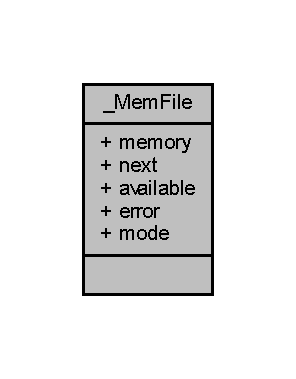
\includegraphics[width=142pt]{struct___mem_file__coll__graph}
\end{center}
\end{figure}
\subsection*{Public 속성}
\begin{DoxyCompactItemize}
\item 
char $\ast$ \mbox{\hyperlink{struct___mem_file_a62a96f96df82e23ef6dace974e19b18c}{memory}}
\item 
char $\ast$ \mbox{\hyperlink{struct___mem_file_aa15859f66ae2eb41245e4ba88486d67f}{next}}
\item 
\mbox{\hyperlink{_util_8cpp_a0ef32aa8672df19503a49fab2d0c8071}{int}} \mbox{\hyperlink{struct___mem_file_a1f48066353e37cf16c9a0065abecf238}{available}}
\item 
\mbox{\hyperlink{_util_8cpp_a0ef32aa8672df19503a49fab2d0c8071}{int}} \mbox{\hyperlink{struct___mem_file_a63100edd8050f287d8dc7070d92a55cb}{error}}
\item 
char \mbox{\hyperlink{struct___mem_file_a88cb51a4419fad64ebfd304b5d0cfe36}{mode}}
\end{DoxyCompactItemize}


\subsection{상세한 설명}


memgzio.\+c 파일의 46 번째 라인에서 정의되었습니다.



\subsection{멤버 데이터 문서화}
\mbox{\Hypertarget{struct___mem_file_a1f48066353e37cf16c9a0065abecf238}\label{struct___mem_file_a1f48066353e37cf16c9a0065abecf238}} 
\index{\+\_\+\+Mem\+File@{\+\_\+\+Mem\+File}!available@{available}}
\index{available@{available}!\+\_\+\+Mem\+File@{\+\_\+\+Mem\+File}}
\subsubsection{\texorpdfstring{available}{available}}
{\footnotesize\ttfamily \mbox{\hyperlink{_util_8cpp_a0ef32aa8672df19503a49fab2d0c8071}{int}} \+\_\+\+Mem\+File\+::available}



memgzio.\+c 파일의 49 번째 라인에서 정의되었습니다.

\mbox{\Hypertarget{struct___mem_file_a63100edd8050f287d8dc7070d92a55cb}\label{struct___mem_file_a63100edd8050f287d8dc7070d92a55cb}} 
\index{\+\_\+\+Mem\+File@{\+\_\+\+Mem\+File}!error@{error}}
\index{error@{error}!\+\_\+\+Mem\+File@{\+\_\+\+Mem\+File}}
\subsubsection{\texorpdfstring{error}{error}}
{\footnotesize\ttfamily \mbox{\hyperlink{_util_8cpp_a0ef32aa8672df19503a49fab2d0c8071}{int}} \+\_\+\+Mem\+File\+::error}



memgzio.\+c 파일의 50 번째 라인에서 정의되었습니다.

\mbox{\Hypertarget{struct___mem_file_a62a96f96df82e23ef6dace974e19b18c}\label{struct___mem_file_a62a96f96df82e23ef6dace974e19b18c}} 
\index{\+\_\+\+Mem\+File@{\+\_\+\+Mem\+File}!memory@{memory}}
\index{memory@{memory}!\+\_\+\+Mem\+File@{\+\_\+\+Mem\+File}}
\subsubsection{\texorpdfstring{memory}{memory}}
{\footnotesize\ttfamily char$\ast$ \+\_\+\+Mem\+File\+::memory}



memgzio.\+c 파일의 47 번째 라인에서 정의되었습니다.

\mbox{\Hypertarget{struct___mem_file_a88cb51a4419fad64ebfd304b5d0cfe36}\label{struct___mem_file_a88cb51a4419fad64ebfd304b5d0cfe36}} 
\index{\+\_\+\+Mem\+File@{\+\_\+\+Mem\+File}!mode@{mode}}
\index{mode@{mode}!\+\_\+\+Mem\+File@{\+\_\+\+Mem\+File}}
\subsubsection{\texorpdfstring{mode}{mode}}
{\footnotesize\ttfamily char \+\_\+\+Mem\+File\+::mode}



memgzio.\+c 파일의 51 번째 라인에서 정의되었습니다.

\mbox{\Hypertarget{struct___mem_file_aa15859f66ae2eb41245e4ba88486d67f}\label{struct___mem_file_aa15859f66ae2eb41245e4ba88486d67f}} 
\index{\+\_\+\+Mem\+File@{\+\_\+\+Mem\+File}!next@{next}}
\index{next@{next}!\+\_\+\+Mem\+File@{\+\_\+\+Mem\+File}}
\subsubsection{\texorpdfstring{next}{next}}
{\footnotesize\ttfamily char$\ast$ \+\_\+\+Mem\+File\+::next}



memgzio.\+c 파일의 48 번째 라인에서 정의되었습니다.



이 구조체에 대한 문서화 페이지는 다음의 파일로부터 생성되었습니다.\+:\begin{DoxyCompactItemize}
\item 
C\+:/\+Users/sjh13/sources/\+Visual\+Boy\+Advance/src/\mbox{\hyperlink{memgzio_8c}{memgzio.\+c}}\end{DoxyCompactItemize}

\hypertarget{class_about_dialog}{}\section{About\+Dialog 클래스 참조}
\label{class_about_dialog}\index{About\+Dialog@{About\+Dialog}}
About\+Dialog에 대한 상속 다이어그램 \+: \begin{figure}[H]
\begin{center}
\leavevmode
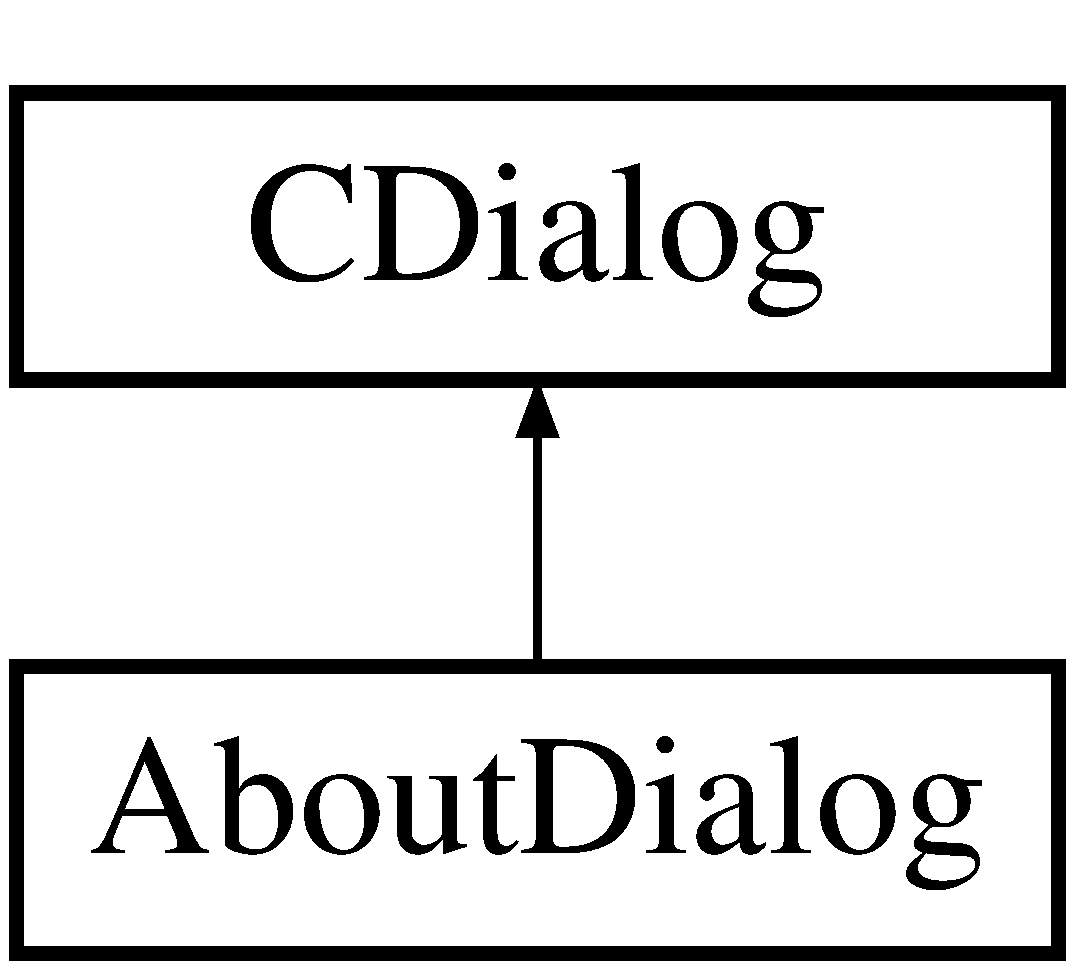
\includegraphics[height=2.000000cm]{class_about_dialog}
\end{center}
\end{figure}
\subsection*{Public 타입}
\begin{DoxyCompactItemize}
\item 
\mbox{\Hypertarget{class_about_dialog_ad39ef53347d21ec0cb70ff40df557e61}\label{class_about_dialog_ad39ef53347d21ec0cb70ff40df557e61}} 
enum \{ {\bfseries I\+DD} = I\+D\+D\+\_\+\+A\+B\+O\+UT
 \}
\end{DoxyCompactItemize}
\subsection*{Public 멤버 함수}
\begin{DoxyCompactItemize}
\item 
\mbox{\Hypertarget{class_about_dialog_a4a8056094af91d12bca94d4fcba1aeae}\label{class_about_dialog_a4a8056094af91d12bca94d4fcba1aeae}} 
{\bfseries About\+Dialog} (C\+Wnd $\ast$p\+Parent=N\+U\+LL)
\end{DoxyCompactItemize}
\subsection*{Public 속성}
\begin{DoxyCompactItemize}
\item 
\mbox{\Hypertarget{class_about_dialog_a78e658a0c2d03632ce86a675b89d8492}\label{class_about_dialog_a78e658a0c2d03632ce86a675b89d8492}} 
C\+String {\bfseries m\+\_\+version}
\end{DoxyCompactItemize}
\subsection*{Protected 멤버 함수}
\begin{DoxyCompactItemize}
\item 
\mbox{\Hypertarget{class_about_dialog_a098f0327b766a8c3fff0fef3076dc9eb}\label{class_about_dialog_a098f0327b766a8c3fff0fef3076dc9eb}} 
virtual void {\bfseries Do\+Data\+Exchange} (C\+Data\+Exchange $\ast$p\+DX)
\item 
\mbox{\Hypertarget{class_about_dialog_ab42eeca93160e48d480b004aaf33c353}\label{class_about_dialog_ab42eeca93160e48d480b004aaf33c353}} 
virtual B\+O\+OL {\bfseries On\+Init\+Dialog} ()
\end{DoxyCompactItemize}


이 클래스에 대한 문서화 페이지는 다음의 파일들로부터 생성되었습니다.\+:\begin{DoxyCompactItemize}
\item 
src/win32/About\+Dialog.\+h\item 
src/win32/About\+Dialog.\+cpp\end{DoxyCompactItemize}

\hypertarget{class_accel_editor}{}\section{Accel\+Editor 클래스 참조}
\label{class_accel_editor}\index{Accel\+Editor@{Accel\+Editor}}


{\ttfamily \#include $<$Accel\+Editor.\+h$>$}



Accel\+Editor에 대한 상속 다이어그램 \+: \nopagebreak
\begin{figure}[H]
\begin{center}
\leavevmode
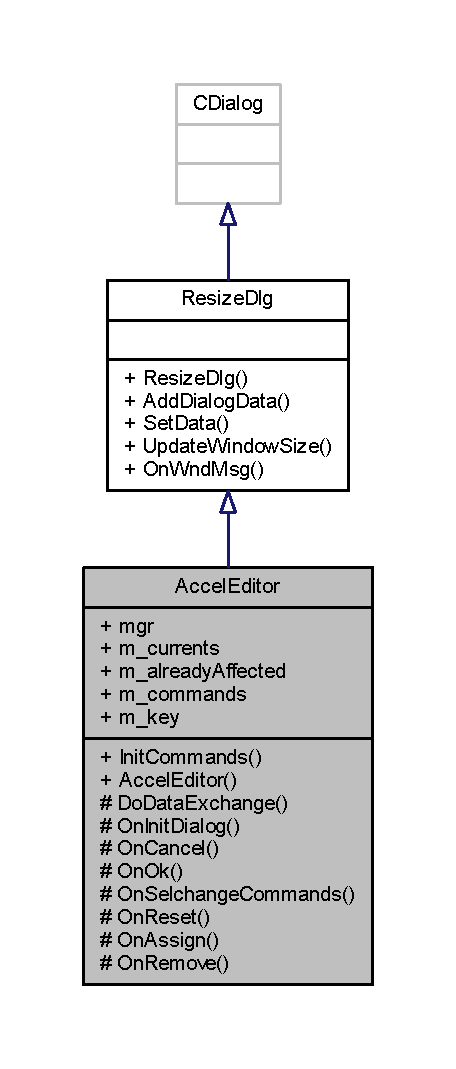
\includegraphics[width=219pt]{class_accel_editor__inherit__graph}
\end{center}
\end{figure}


Accel\+Editor에 대한 협력 다이어그램\+:\nopagebreak
\begin{figure}[H]
\begin{center}
\leavevmode
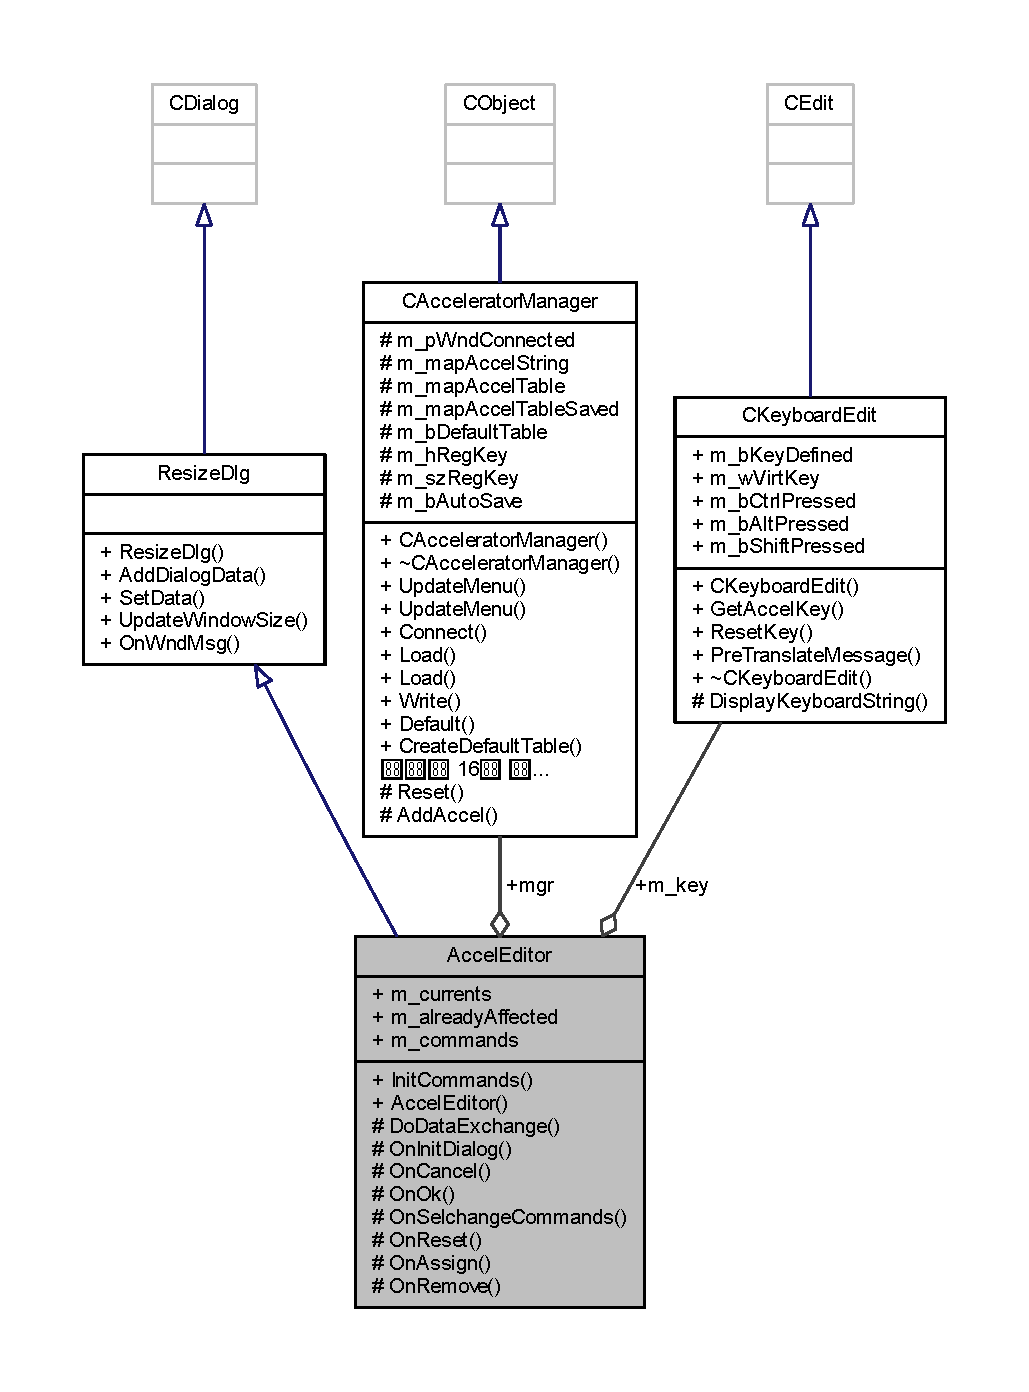
\includegraphics[width=350pt]{class_accel_editor__coll__graph}
\end{center}
\end{figure}
\subsection*{Public 타입}
\begin{DoxyCompactItemize}
\item 
enum \{ \mbox{\hyperlink{class_accel_editor_a2c120196c6edcc4e45a1eb6321060cf7a3ed38c6627e19d20129d5a6eee67408c}{I\+DD}} = I\+D\+D\+\_\+\+A\+C\+C\+E\+L\+\_\+\+E\+D\+I\+T\+OR
 \}
\end{DoxyCompactItemize}
\subsection*{Public 멤버 함수}
\begin{DoxyCompactItemize}
\item 
void \mbox{\hyperlink{class_accel_editor_a3c882fb85c72711e26cfe800fb11ccfa}{Init\+Commands}} ()
\item 
\mbox{\hyperlink{class_accel_editor_a4f3eb3bfb01a597da630a3144687f1ec}{Accel\+Editor}} (C\+Wnd $\ast$p\+Parent=\mbox{\hyperlink{_system_8h_a070d2ce7b6bb7e5c05602aa8c308d0c4}{N\+U\+LL}})
\end{DoxyCompactItemize}
\subsection*{Public 속성}
\begin{DoxyCompactItemize}
\item 
\mbox{\hyperlink{class_c_accelerator_manager}{C\+Accelerator\+Manager}} \mbox{\hyperlink{class_accel_editor_acb731e2193cb5022a95e83122651f96d}{mgr}}
\item 
C\+List\+Box \mbox{\hyperlink{class_accel_editor_a31909da8a929ef7b5e22ffbf64f1c68c}{m\+\_\+currents}}
\item 
C\+Static \mbox{\hyperlink{class_accel_editor_ac3d2378be850611ee51689bd34475275}{m\+\_\+already\+Affected}}
\item 
C\+List\+Box \mbox{\hyperlink{class_accel_editor_aba4ea3d3eced08de9fe39e307b5f40fc}{m\+\_\+commands}}
\item 
\mbox{\hyperlink{class_c_keyboard_edit}{C\+Keyboard\+Edit}} \mbox{\hyperlink{class_accel_editor_af0875f914fdddf5233a951cabd499a4d}{m\+\_\+key}}
\end{DoxyCompactItemize}
\subsection*{Protected 멤버 함수}
\begin{DoxyCompactItemize}
\item 
virtual void \mbox{\hyperlink{class_accel_editor_a3212b434e8c489ba308fa6a474dd32e7}{Do\+Data\+Exchange}} (C\+Data\+Exchange $\ast$p\+DX)
\item 
virtual B\+O\+OL \mbox{\hyperlink{class_accel_editor_a131b32f139220aadd5e36b4ddeb8cd58}{On\+Init\+Dialog}} ()
\item 
afx\+\_\+msg void \mbox{\hyperlink{class_accel_editor_a50b1043d4af01df3925f193b7755c05e}{On\+Cancel}} ()
\item 
afx\+\_\+msg void \mbox{\hyperlink{class_accel_editor_a3afd18b4482500a4ea29ee5d0d43cffc}{On\+Ok}} ()
\item 
afx\+\_\+msg void \mbox{\hyperlink{class_accel_editor_a16cb5c73f55199115c5a4f35268ff3fa}{On\+Selchange\+Commands}} ()
\item 
afx\+\_\+msg void \mbox{\hyperlink{class_accel_editor_a1afed0a04125915ae1517e1b08879b8b}{On\+Reset}} ()
\item 
afx\+\_\+msg void \mbox{\hyperlink{class_accel_editor_ad33ae69dcc262dd73595cb33d82c209e}{On\+Assign}} ()
\item 
afx\+\_\+msg void \mbox{\hyperlink{class_accel_editor_a40b74b67b95694245502b15ceedd278c}{On\+Remove}} ()
\end{DoxyCompactItemize}


\subsection{상세한 설명}


Accel\+Editor.\+h 파일의 35 번째 라인에서 정의되었습니다.



\subsection{멤버 열거형 문서화}
\mbox{\Hypertarget{class_accel_editor_a2c120196c6edcc4e45a1eb6321060cf7}\label{class_accel_editor_a2c120196c6edcc4e45a1eb6321060cf7}} 
\subsubsection{\texorpdfstring{anonymous enum}{anonymous enum}}
{\footnotesize\ttfamily anonymous enum}

\begin{DoxyEnumFields}{열거형 멤버}
\raisebox{\heightof{T}}[0pt][0pt]{\index{I\+DD@{I\+DD}!Accel\+Editor@{Accel\+Editor}}\index{Accel\+Editor@{Accel\+Editor}!I\+DD@{I\+DD}}}\mbox{\Hypertarget{class_accel_editor_a2c120196c6edcc4e45a1eb6321060cf7a3ed38c6627e19d20129d5a6eee67408c}\label{class_accel_editor_a2c120196c6edcc4e45a1eb6321060cf7a3ed38c6627e19d20129d5a6eee67408c}} 
I\+DD&\\
\hline

\end{DoxyEnumFields}


Accel\+Editor.\+h 파일의 45 번째 라인에서 정의되었습니다.


\begin{DoxyCode}
45 \{ \mbox{\hyperlink{class_accel_editor_a2c120196c6edcc4e45a1eb6321060cf7a3ed38c6627e19d20129d5a6eee67408c}{IDD}} = \mbox{\hyperlink{resource_8h_a5244accea8f995e6b35d0dcc7572b379}{IDD\_ACCEL\_EDITOR}} \};
\end{DoxyCode}


\subsection{생성자 \& 소멸자 문서화}
\mbox{\Hypertarget{class_accel_editor_a4f3eb3bfb01a597da630a3144687f1ec}\label{class_accel_editor_a4f3eb3bfb01a597da630a3144687f1ec}} 
\index{Accel\+Editor@{Accel\+Editor}!Accel\+Editor@{Accel\+Editor}}
\index{Accel\+Editor@{Accel\+Editor}!Accel\+Editor@{Accel\+Editor}}
\subsubsection{\texorpdfstring{Accel\+Editor()}{AccelEditor()}}
{\footnotesize\ttfamily Accel\+Editor\+::\+Accel\+Editor (\begin{DoxyParamCaption}\item[{C\+Wnd $\ast$}]{p\+Parent = {\ttfamily \mbox{\hyperlink{_system_8h_a070d2ce7b6bb7e5c05602aa8c308d0c4}{N\+U\+LL}}} }\end{DoxyParamCaption})}



Accel\+Editor.\+cpp 파일의 37 번째 라인에서 정의되었습니다.


\begin{DoxyCode}
38   : \mbox{\hyperlink{class_resize_dlg_a87bab778e9312f274ebe750d4c3a67ee}{ResizeDlg}}(\mbox{\hyperlink{class_accel_editor_a2c120196c6edcc4e45a1eb6321060cf7a3ed38c6627e19d20129d5a6eee67408c}{AccelEditor::IDD}}, pParent)
39 \{
40   \textcolor{comment}{//\{\{AFX\_DATA\_INIT(AccelEditor)}
41   \textcolor{comment}{// NOTE: the ClassWizard will add member initialization here}
42   \textcolor{comment}{//\}\}AFX\_DATA\_INIT}
43   \mbox{\hyperlink{class_accel_editor_acb731e2193cb5022a95e83122651f96d}{mgr}} = \mbox{\hyperlink{_v_b_a_8cpp_a8095a9d06b37a7efe3723f3218ad8fb3}{theApp}}.\mbox{\hyperlink{class_v_b_a_ad7ebce057dbde0ca88cee75e84721a89}{winAccelMgr}};
44 \}
\end{DoxyCode}


\subsection{멤버 함수 문서화}
\mbox{\Hypertarget{class_accel_editor_a3212b434e8c489ba308fa6a474dd32e7}\label{class_accel_editor_a3212b434e8c489ba308fa6a474dd32e7}} 
\index{Accel\+Editor@{Accel\+Editor}!Do\+Data\+Exchange@{Do\+Data\+Exchange}}
\index{Do\+Data\+Exchange@{Do\+Data\+Exchange}!Accel\+Editor@{Accel\+Editor}}
\subsubsection{\texorpdfstring{Do\+Data\+Exchange()}{DoDataExchange()}}
{\footnotesize\ttfamily void Accel\+Editor\+::\+Do\+Data\+Exchange (\begin{DoxyParamCaption}\item[{C\+Data\+Exchange $\ast$}]{p\+DX }\end{DoxyParamCaption})\hspace{0.3cm}{\ttfamily [protected]}, {\ttfamily [virtual]}}



Accel\+Editor.\+cpp 파일의 47 번째 라인에서 정의되었습니다.


\begin{DoxyCode}
48 \{
49   CDialog::DoDataExchange(pDX);
50   \textcolor{comment}{//\{\{AFX\_DATA\_MAP(AccelEditor)}
51   DDX\_Control(pDX, \mbox{\hyperlink{resource_8h_aecf06df6d523df832c4125d6511946ae}{IDC\_CURRENTS}}, \mbox{\hyperlink{class_accel_editor_a31909da8a929ef7b5e22ffbf64f1c68c}{m\_currents}});
52   DDX\_Control(pDX, \mbox{\hyperlink{resource_8h_ac348623d1b045f612bab36c7899d9507}{IDC\_ALREADY\_AFFECTED}}, \mbox{\hyperlink{class_accel_editor_ac3d2378be850611ee51689bd34475275}{m\_alreadyAffected}});
53   DDX\_Control(pDX, \mbox{\hyperlink{resource_8h_abc997c435dcb4d0b7fd9d34b51a905f1}{IDC\_COMMANDS}}, \mbox{\hyperlink{class_accel_editor_aba4ea3d3eced08de9fe39e307b5f40fc}{m\_commands}});
54   DDX\_Control(pDX, \mbox{\hyperlink{resource_8h_a5c53f670221b594a3fd960d7bc18325d}{IDC\_EDIT\_KEY}}, \mbox{\hyperlink{class_accel_editor_af0875f914fdddf5233a951cabd499a4d}{m\_key}});
55   \textcolor{comment}{//\}\}AFX\_DATA\_MAP}
56 \}
\end{DoxyCode}
\mbox{\Hypertarget{class_accel_editor_a3c882fb85c72711e26cfe800fb11ccfa}\label{class_accel_editor_a3c882fb85c72711e26cfe800fb11ccfa}} 
\index{Accel\+Editor@{Accel\+Editor}!Init\+Commands@{Init\+Commands}}
\index{Init\+Commands@{Init\+Commands}!Accel\+Editor@{Accel\+Editor}}
\subsubsection{\texorpdfstring{Init\+Commands()}{InitCommands()}}
{\footnotesize\ttfamily void Accel\+Editor\+::\+Init\+Commands (\begin{DoxyParamCaption}{ }\end{DoxyParamCaption})}



Accel\+Editor.\+cpp 파일의 105 번째 라인에서 정의되었습니다.


\begin{DoxyCode}
106 \{
107   \mbox{\hyperlink{class_accel_editor_aba4ea3d3eced08de9fe39e307b5f40fc}{m\_commands}}.ResetContent();
108   \mbox{\hyperlink{class_accel_editor_ac3d2378be850611ee51689bd34475275}{m\_alreadyAffected}}.SetWindowText(\textcolor{stringliteral}{""});
109 
110   POSITION pos = \mbox{\hyperlink{class_accel_editor_acb731e2193cb5022a95e83122651f96d}{mgr}}.\mbox{\hyperlink{class_c_accelerator_manager_abb40dbb1a44c47ac22590e8f1243835b}{m\_mapAccelString}}.GetStartPosition();
111   
112   \textcolor{keywordflow}{while}(pos != \mbox{\hyperlink{getopt1_8c_a070d2ce7b6bb7e5c05602aa8c308d0c4}{NULL}}) \{
113     CString \mbox{\hyperlink{_commands_8cpp_a9f83d3c4b4c3bb790f90ad79865e37ab}{command}};
114     WORD wID;
115     \mbox{\hyperlink{class_accel_editor_acb731e2193cb5022a95e83122651f96d}{mgr}}.\mbox{\hyperlink{class_c_accelerator_manager_abb40dbb1a44c47ac22590e8f1243835b}{m\_mapAccelString}}.GetNextAssoc(pos, \mbox{\hyperlink{_commands_8cpp_a9f83d3c4b4c3bb790f90ad79865e37ab}{command}}, wID);
116 
117     \textcolor{keywordtype}{int} index = \mbox{\hyperlink{class_accel_editor_aba4ea3d3eced08de9fe39e307b5f40fc}{m\_commands}}.AddString(\mbox{\hyperlink{_commands_8cpp_a9f83d3c4b4c3bb790f90ad79865e37ab}{command}});
118     \mbox{\hyperlink{class_accel_editor_aba4ea3d3eced08de9fe39e307b5f40fc}{m\_commands}}.SetItemData(index, wID);
119   \}
120 
121   \textcolor{comment}{// Update the currents accels associated with the selected command}
122   \textcolor{keywordflow}{if} (\mbox{\hyperlink{class_accel_editor_aba4ea3d3eced08de9fe39e307b5f40fc}{m\_commands}}.SetCurSel(0) != LB\_ERR)
123     \mbox{\hyperlink{class_accel_editor_a16cb5c73f55199115c5a4f35268ff3fa}{OnSelchangeCommands}}();
124 \}
\end{DoxyCode}
이 함수 내부에서 호출하는 함수들에 대한 그래프입니다.\+:
\nopagebreak
\begin{figure}[H]
\begin{center}
\leavevmode
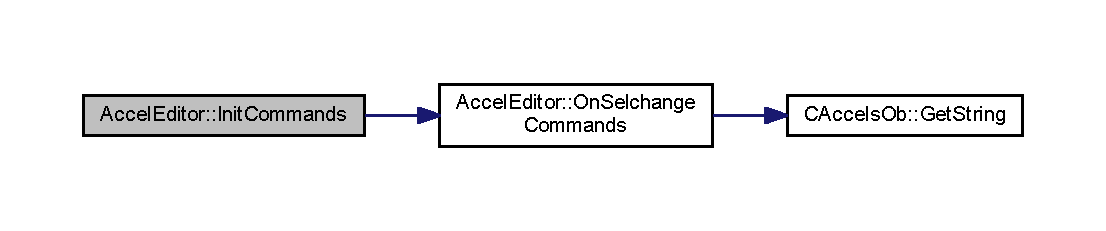
\includegraphics[width=350pt]{class_accel_editor_a3c882fb85c72711e26cfe800fb11ccfa_cgraph}
\end{center}
\end{figure}
이 함수를 호출하는 함수들에 대한 그래프입니다.\+:
\nopagebreak
\begin{figure}[H]
\begin{center}
\leavevmode
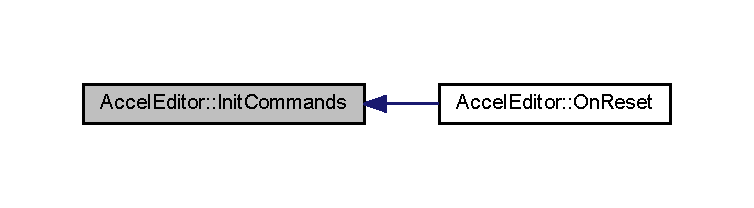
\includegraphics[width=350pt]{class_accel_editor_a3c882fb85c72711e26cfe800fb11ccfa_icgraph}
\end{center}
\end{figure}
\mbox{\Hypertarget{class_accel_editor_ad33ae69dcc262dd73595cb33d82c209e}\label{class_accel_editor_ad33ae69dcc262dd73595cb33d82c209e}} 
\index{Accel\+Editor@{Accel\+Editor}!On\+Assign@{On\+Assign}}
\index{On\+Assign@{On\+Assign}!Accel\+Editor@{Accel\+Editor}}
\subsubsection{\texorpdfstring{On\+Assign()}{OnAssign()}}
{\footnotesize\ttfamily void Accel\+Editor\+::\+On\+Assign (\begin{DoxyParamCaption}{ }\end{DoxyParamCaption})\hspace{0.3cm}{\ttfamily [protected]}}



Accel\+Editor.\+cpp 파일의 173 번째 라인에서 정의되었습니다.


\begin{DoxyCode}
174 \{
175   \textcolor{comment}{// Control if it's not already affected}
176   \mbox{\hyperlink{class_c_cmd_accel_ob}{CCmdAccelOb}}* pCmdAccel;
177   \mbox{\hyperlink{class_c_accels_ob}{CAccelsOb}}* pAccel;
178   WORD wIDCommand;
179   POSITION pos;
180   
181   WORD wKey;
182   \textcolor{keywordtype}{bool} bCtrl, bAlt, bShift;
183 
184   \textcolor{keywordflow}{if} (!\mbox{\hyperlink{class_accel_editor_af0875f914fdddf5233a951cabd499a4d}{m\_key}}.\mbox{\hyperlink{class_c_keyboard_edit_a920dfccebef5e2260e59003e4959ef9f}{GetAccelKey}}(wKey, bCtrl, bAlt, bShift))
185     \textcolor{keywordflow}{return}; \textcolor{comment}{// no valid key, abort}
186 
187   \textcolor{keywordtype}{int} \mbox{\hyperlink{expr_8cpp_a16ff2d8e15ade4948398b0aeb80124a8}{count}} = \mbox{\hyperlink{class_accel_editor_aba4ea3d3eced08de9fe39e307b5f40fc}{m\_commands}}.GetCount();
188   \textcolor{keywordtype}{int} index;
189   \textcolor{keywordflow}{for} (index = 0; index < \mbox{\hyperlink{expr_8cpp_a16ff2d8e15ade4948398b0aeb80124a8}{count}}; index++) \{
190 
191     wIDCommand = LOWORD(\mbox{\hyperlink{class_accel_editor_aba4ea3d3eced08de9fe39e307b5f40fc}{m\_commands}}.GetItemData(index));
192     \mbox{\hyperlink{class_accel_editor_acb731e2193cb5022a95e83122651f96d}{mgr}}.\mbox{\hyperlink{class_c_accelerator_manager_a16b8d3e9328bc0eeeb048630deff2768}{m\_mapAccelTable}}.Lookup(wIDCommand, pCmdAccel);
193 
194     pos = pCmdAccel->\mbox{\hyperlink{class_c_cmd_accel_ob_a85772f1ea9204af42b8a39a0135dc0f8}{m\_Accels}}.GetHeadPosition();
195     \textcolor{keywordflow}{while} (pos != \mbox{\hyperlink{getopt1_8c_a070d2ce7b6bb7e5c05602aa8c308d0c4}{NULL}}) \{
196       pAccel = pCmdAccel->\mbox{\hyperlink{class_c_cmd_accel_ob_a85772f1ea9204af42b8a39a0135dc0f8}{m\_Accels}}.GetNext(pos);
197       \textcolor{keywordflow}{if} (pAccel->\mbox{\hyperlink{class_c_accels_ob_a32714a4454d398d3d3a68d1705a76bc5}{IsEqual}}(wKey, bCtrl, bAlt, bShift)) \{
198         \textcolor{comment}{// the key is already affected (in the same or other command)}
199         \mbox{\hyperlink{class_accel_editor_ac3d2378be850611ee51689bd34475275}{m\_alreadyAffected}}.SetWindowText(pCmdAccel->\mbox{\hyperlink{class_c_cmd_accel_ob_acbd02cc68d3909b1e39b687e76f45d91}{m\_szCommand}});
200         \mbox{\hyperlink{class_accel_editor_af0875f914fdddf5233a951cabd499a4d}{m\_key}}.SetSel(0, -1);
201         \textcolor{keywordflow}{return}; \textcolor{comment}{// abort}
202       \}
203     \}
204   \}
205 
206   \textcolor{comment}{// OK, we can add the accel key in the currently selected group}
207   index = \mbox{\hyperlink{class_accel_editor_aba4ea3d3eced08de9fe39e307b5f40fc}{m\_commands}}.GetCurSel();
208   \textcolor{keywordflow}{if} (index == LB\_ERR)
209     \textcolor{keywordflow}{return};
210 
211   \textcolor{comment}{// Get the object who manage the accels list, associated to the command.}
212   wIDCommand = LOWORD(\mbox{\hyperlink{class_accel_editor_aba4ea3d3eced08de9fe39e307b5f40fc}{m\_commands}}.GetItemData(index));
213 
214   \textcolor{keywordflow}{if} (\mbox{\hyperlink{class_accel_editor_acb731e2193cb5022a95e83122651f96d}{mgr}}.\mbox{\hyperlink{class_c_accelerator_manager_a16b8d3e9328bc0eeeb048630deff2768}{m\_mapAccelTable}}.Lookup(wIDCommand, pCmdAccel) != TRUE)
215     \textcolor{keywordflow}{return};
216 
217   BYTE cVirt = 0;
218   \textcolor{keywordflow}{if} (bCtrl)
219     cVirt |= FCONTROL;
220   \textcolor{keywordflow}{if} (bAlt)
221     cVirt |= FALT;
222   \textcolor{keywordflow}{if} (bShift)
223     cVirt |= FSHIFT;
224 
225   cVirt |= FVIRTKEY;
226 
227   \textcolor{comment}{// Create the new key...}
228   pAccel = \textcolor{keyword}{new} \mbox{\hyperlink{class_c_accels_ob}{CAccelsOb}}(cVirt, wKey, \textcolor{keyword}{false});
229   ASSERT(pAccel != \mbox{\hyperlink{getopt1_8c_a070d2ce7b6bb7e5c05602aa8c308d0c4}{NULL}});
230   \textcolor{comment}{// ...and add in the list.}
231   pCmdAccel->\mbox{\hyperlink{class_c_cmd_accel_ob_a85772f1ea9204af42b8a39a0135dc0f8}{m\_Accels}}.AddTail(pAccel);
232 
233   \textcolor{comment}{// Update the listbox.}
234   CString szBuffer;
235   pAccel->\mbox{\hyperlink{class_c_accels_ob_afaf7510fa1e0707863f6bd469f190de6}{GetString}}(szBuffer);
236 
237   index = \mbox{\hyperlink{class_accel_editor_a31909da8a929ef7b5e22ffbf64f1c68c}{m\_currents}}.AddString(szBuffer);
238   \mbox{\hyperlink{class_accel_editor_a31909da8a929ef7b5e22ffbf64f1c68c}{m\_currents}}.SetItemData(index, (DWORD\_PTR)pAccel);
239 
240   \textcolor{comment}{// Reset the key editor.}
241   \mbox{\hyperlink{class_accel_editor_af0875f914fdddf5233a951cabd499a4d}{m\_key}}.\mbox{\hyperlink{class_c_keyboard_edit_ad0185cc0cad77250cc32ef1d9ffb8593}{ResetKey}}();
242 \}
\end{DoxyCode}
이 함수 내부에서 호출하는 함수들에 대한 그래프입니다.\+:
\nopagebreak
\begin{figure}[H]
\begin{center}
\leavevmode
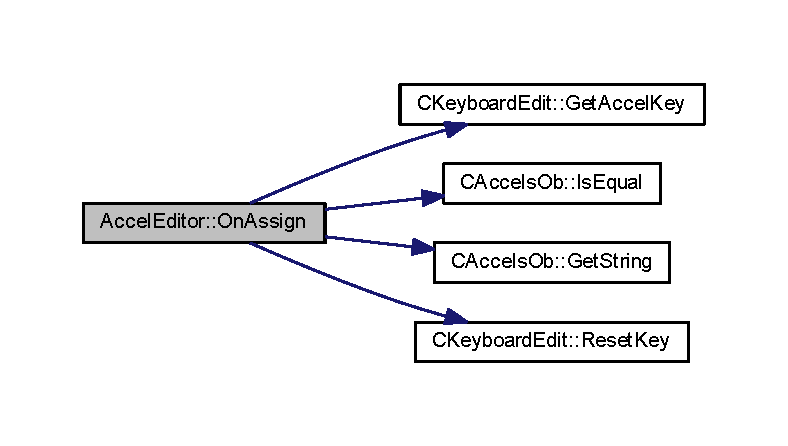
\includegraphics[width=350pt]{class_accel_editor_ad33ae69dcc262dd73595cb33d82c209e_cgraph}
\end{center}
\end{figure}
\mbox{\Hypertarget{class_accel_editor_a50b1043d4af01df3925f193b7755c05e}\label{class_accel_editor_a50b1043d4af01df3925f193b7755c05e}} 
\index{Accel\+Editor@{Accel\+Editor}!On\+Cancel@{On\+Cancel}}
\index{On\+Cancel@{On\+Cancel}!Accel\+Editor@{Accel\+Editor}}
\subsubsection{\texorpdfstring{On\+Cancel()}{OnCancel()}}
{\footnotesize\ttfamily void Accel\+Editor\+::\+On\+Cancel (\begin{DoxyParamCaption}{ }\end{DoxyParamCaption})\hspace{0.3cm}{\ttfamily [protected]}}



Accel\+Editor.\+cpp 파일의 126 번째 라인에서 정의되었습니다.


\begin{DoxyCode}
127 \{
128   EndDialog(FALSE);
129 \}
\end{DoxyCode}
\mbox{\Hypertarget{class_accel_editor_a131b32f139220aadd5e36b4ddeb8cd58}\label{class_accel_editor_a131b32f139220aadd5e36b4ddeb8cd58}} 
\index{Accel\+Editor@{Accel\+Editor}!On\+Init\+Dialog@{On\+Init\+Dialog}}
\index{On\+Init\+Dialog@{On\+Init\+Dialog}!Accel\+Editor@{Accel\+Editor}}
\subsubsection{\texorpdfstring{On\+Init\+Dialog()}{OnInitDialog()}}
{\footnotesize\ttfamily B\+O\+OL Accel\+Editor\+::\+On\+Init\+Dialog (\begin{DoxyParamCaption}{ }\end{DoxyParamCaption})\hspace{0.3cm}{\ttfamily [protected]}, {\ttfamily [virtual]}}



Accel\+Editor.\+cpp 파일의 73 번째 라인에서 정의되었습니다.


\begin{DoxyCode}
74 \{
75   CDialog::OnInitDialog();
76   
77   \mbox{\hyperlink{_resize_dlg_8h_acb9d1d22d9838f6dda8a61cfa132997c}{DIALOG\_SIZER\_START}}( sz )
78     \mbox{\hyperlink{_resize_dlg_8h_a0e9ee7a18c54003893895a009f5d79c8}{DIALOG\_SIZER\_ENTRY}}( \mbox{\hyperlink{resource_8h_a37f587596b464239581b844e04dda1da}{IDC\_STATIC1}}, \mbox{\hyperlink{_resize_dlg_8h_a9f96d817606755d91347bd606825c5af}{DS\_MoveX}})
79     \mbox{\hyperlink{_resize_dlg_8h_a0e9ee7a18c54003893895a009f5d79c8}{DIALOG\_SIZER\_ENTRY}}( \mbox{\hyperlink{resource_8h_acdec4653db2f21850f3ee1f41c3c0080}{IDC\_STATIC2}}, \mbox{\hyperlink{_resize_dlg_8h_ae5309071be822a4dae5cb33a131f6180}{DS\_MoveY}})
80     \mbox{\hyperlink{_resize_dlg_8h_a0e9ee7a18c54003893895a009f5d79c8}{DIALOG\_SIZER\_ENTRY}}( \mbox{\hyperlink{resource_8h_a62cedae02f3076f30d9a6bb0ed8d3e43}{IDC\_STATIC3}}, \mbox{\hyperlink{_resize_dlg_8h_a9f96d817606755d91347bd606825c5af}{DS\_MoveX}} | 
      \mbox{\hyperlink{_resize_dlg_8h_ae5309071be822a4dae5cb33a131f6180}{DS\_MoveY}})
81     \mbox{\hyperlink{_resize_dlg_8h_a0e9ee7a18c54003893895a009f5d79c8}{DIALOG\_SIZER\_ENTRY}}( \mbox{\hyperlink{resource_8h_ac348623d1b045f612bab36c7899d9507}{IDC\_ALREADY\_AFFECTED}}, 
      \mbox{\hyperlink{_resize_dlg_8h_ae5309071be822a4dae5cb33a131f6180}{DS\_MoveY}})
82     \mbox{\hyperlink{_resize_dlg_8h_a0e9ee7a18c54003893895a009f5d79c8}{DIALOG\_SIZER\_ENTRY}}( \mbox{\hyperlink{resource_8h_a4cf7b8af561e85b223c39c4c2b22ef18}{ID\_OK}}, \mbox{\hyperlink{_resize_dlg_8h_a9f96d817606755d91347bd606825c5af}{DS\_MoveX}})
83     \mbox{\hyperlink{_resize_dlg_8h_a0e9ee7a18c54003893895a009f5d79c8}{DIALOG\_SIZER\_ENTRY}}( \mbox{\hyperlink{resource_8h_a9f066b92f1c9e4f0f0a679d67fd29d31}{ID\_CANCEL}}, \mbox{\hyperlink{_resize_dlg_8h_a9f96d817606755d91347bd606825c5af}{DS\_MoveX}})
84     \mbox{\hyperlink{_resize_dlg_8h_a0e9ee7a18c54003893895a009f5d79c8}{DIALOG\_SIZER\_ENTRY}}( \mbox{\hyperlink{resource_8h_a80cc1cf3d03957bcb73aba8214c3d319}{IDC\_ASSIGN}}, \mbox{\hyperlink{_resize_dlg_8h_a9f96d817606755d91347bd606825c5af}{DS\_MoveX}})
85     \mbox{\hyperlink{_resize_dlg_8h_a0e9ee7a18c54003893895a009f5d79c8}{DIALOG\_SIZER\_ENTRY}}( \mbox{\hyperlink{resource_8h_aa8441a495432bef29886eed49bbaa08c}{IDC\_REMOVE}}, \mbox{\hyperlink{_resize_dlg_8h_a9f96d817606755d91347bd606825c5af}{DS\_MoveX}})
86     \mbox{\hyperlink{_resize_dlg_8h_a0e9ee7a18c54003893895a009f5d79c8}{DIALOG\_SIZER\_ENTRY}}( \mbox{\hyperlink{resource_8h_ac19883430c1a49f08af98721f02d95eb}{IDC\_RESET}}, \mbox{\hyperlink{_resize_dlg_8h_a9f96d817606755d91347bd606825c5af}{DS\_MoveX}})
87     \mbox{\hyperlink{_resize_dlg_8h_a0e9ee7a18c54003893895a009f5d79c8}{DIALOG\_SIZER\_ENTRY}}( \mbox{\hyperlink{resource_8h_a27e7224faecfa4040c695a69107088f9}{IDC\_CLOSE}}, \mbox{\hyperlink{_resize_dlg_8h_ae5309071be822a4dae5cb33a131f6180}{DS\_MoveY}})
88     \mbox{\hyperlink{_resize_dlg_8h_a0e9ee7a18c54003893895a009f5d79c8}{DIALOG\_SIZER\_ENTRY}}( \mbox{\hyperlink{resource_8h_abc997c435dcb4d0b7fd9d34b51a905f1}{IDC\_COMMANDS}}, \mbox{\hyperlink{_resize_dlg_8h_a21713fd373c62604a1ee3d5d831101ad}{DS\_SizeX}} | 
      \mbox{\hyperlink{_resize_dlg_8h_a783821ba6bb984916d55f46cdf90cb2b}{DS\_SizeY}})
89     \mbox{\hyperlink{_resize_dlg_8h_a0e9ee7a18c54003893895a009f5d79c8}{DIALOG\_SIZER\_ENTRY}}( \mbox{\hyperlink{resource_8h_aecf06df6d523df832c4125d6511946ae}{IDC\_CURRENTS}}, \mbox{\hyperlink{_resize_dlg_8h_a9f96d817606755d91347bd606825c5af}{DS\_MoveX}} | 
      \mbox{\hyperlink{_resize_dlg_8h_a783821ba6bb984916d55f46cdf90cb2b}{DS\_SizeY}})
90     \mbox{\hyperlink{_resize_dlg_8h_a0e9ee7a18c54003893895a009f5d79c8}{DIALOG\_SIZER\_ENTRY}}( \mbox{\hyperlink{resource_8h_a5c53f670221b594a3fd960d7bc18325d}{IDC\_EDIT\_KEY}}, \mbox{\hyperlink{_resize_dlg_8h_a9f96d817606755d91347bd606825c5af}{DS\_MoveX}} | 
      \mbox{\hyperlink{_resize_dlg_8h_ae5309071be822a4dae5cb33a131f6180}{DS\_MoveY}})
91     \mbox{\hyperlink{_resize_dlg_8h_aeac0c1e32f30e0763df5736e4b3ea50a}{DIALOG\_SIZER\_END}}()
92 
93     \mbox{\hyperlink{class_resize_dlg_a6a3965f44a0c2f5ba9aaa798a9a81df5}{SetData}}(sz,
94             TRUE,
95             HKEY\_CURRENT\_USER,
96             "Software\(\backslash\)\(\backslash\)Emulators\(\backslash\)\(\backslash\)VisualBoyAdvance\(\backslash\)\(\backslash\)Viewer\(\backslash\)\(\backslash\)\mbox{\hyperlink{class_accel_editor}{AccelEditor}}",
97             \mbox{\hyperlink{getopt1_8c_a070d2ce7b6bb7e5c05602aa8c308d0c4}{NULL}});
98 
99   \mbox{\hyperlink{class_accel_editor_a3c882fb85c72711e26cfe800fb11ccfa}{InitCommands}}();
100   
101   \mbox{\hyperlink{gb_codes_8h_a9717e7bbecb906637e86cef6da3d83c2}{return}} TRUE;  \textcolor{comment}{// return TRUE unless you set the focus to a control}
102                 \textcolor{comment}{// EXCEPTION: OCX Property Pages should return FALSE}
103 \}
\end{DoxyCode}
\mbox{\Hypertarget{class_accel_editor_a3afd18b4482500a4ea29ee5d0d43cffc}\label{class_accel_editor_a3afd18b4482500a4ea29ee5d0d43cffc}} 
\index{Accel\+Editor@{Accel\+Editor}!On\+Ok@{On\+Ok}}
\index{On\+Ok@{On\+Ok}!Accel\+Editor@{Accel\+Editor}}
\subsubsection{\texorpdfstring{On\+Ok()}{OnOk()}}
{\footnotesize\ttfamily void Accel\+Editor\+::\+On\+Ok (\begin{DoxyParamCaption}{ }\end{DoxyParamCaption})\hspace{0.3cm}{\ttfamily [protected]}}



Accel\+Editor.\+cpp 파일의 131 번째 라인에서 정의되었습니다.


\begin{DoxyCode}
132 \{
133   EndDialog(TRUE);
134 \}
\end{DoxyCode}
\mbox{\Hypertarget{class_accel_editor_a40b74b67b95694245502b15ceedd278c}\label{class_accel_editor_a40b74b67b95694245502b15ceedd278c}} 
\index{Accel\+Editor@{Accel\+Editor}!On\+Remove@{On\+Remove}}
\index{On\+Remove@{On\+Remove}!Accel\+Editor@{Accel\+Editor}}
\subsubsection{\texorpdfstring{On\+Remove()}{OnRemove()}}
{\footnotesize\ttfamily void Accel\+Editor\+::\+On\+Remove (\begin{DoxyParamCaption}{ }\end{DoxyParamCaption})\hspace{0.3cm}{\ttfamily [protected]}}



Accel\+Editor.\+cpp 파일의 244 번째 라인에서 정의되었습니다.


\begin{DoxyCode}
245 \{
246   \textcolor{comment}{// Some controls}
247   \textcolor{keywordtype}{int} indexCurrent = \mbox{\hyperlink{class_accel_editor_a31909da8a929ef7b5e22ffbf64f1c68c}{m\_currents}}.GetCurSel();
248   \textcolor{keywordflow}{if} (indexCurrent == LB\_ERR)
249     \textcolor{keywordflow}{return};
250   
251   \textcolor{comment}{// 2nd part.}
252   \textcolor{keywordtype}{int} indexCmd = \mbox{\hyperlink{class_accel_editor_aba4ea3d3eced08de9fe39e307b5f40fc}{m\_commands}}.GetCurSel();
253   \textcolor{keywordflow}{if} (indexCmd == LB\_ERR)
254     \textcolor{keywordflow}{return};
255 
256   \textcolor{comment}{// Ref to the ID command}
257   WORD wIDCommand = LOWORD(\mbox{\hyperlink{class_accel_editor_aba4ea3d3eced08de9fe39e307b5f40fc}{m\_commands}}.GetItemData(indexCmd));
258 
259   \textcolor{comment}{// Run through the accels,and control if it can be deleted.}
260   \mbox{\hyperlink{class_c_cmd_accel_ob}{CCmdAccelOb}}* pCmdAccel;
261   \textcolor{keywordflow}{if} (\mbox{\hyperlink{class_accel_editor_acb731e2193cb5022a95e83122651f96d}{mgr}}.\mbox{\hyperlink{class_c_accelerator_manager_a16b8d3e9328bc0eeeb048630deff2768}{m\_mapAccelTable}}.Lookup(wIDCommand, pCmdAccel) == TRUE) \{
262     \mbox{\hyperlink{class_c_accels_ob}{CAccelsOb}}* pAccel;
263     \mbox{\hyperlink{class_c_accels_ob}{CAccelsOb}}* pAccelCurrent = (\mbox{\hyperlink{class_c_accels_ob}{CAccelsOb}}*)(\mbox{\hyperlink{class_accel_editor_a31909da8a929ef7b5e22ffbf64f1c68c}{m\_currents}}.GetItemData(indexCurrent
      ));
264     CString szBuffer;
265     POSITION pos = pCmdAccel->m\_Accels.GetHeadPosition();
266     POSITION PrevPos;
267     \textcolor{keywordflow}{while} (pos != \mbox{\hyperlink{getopt1_8c_a070d2ce7b6bb7e5c05602aa8c308d0c4}{NULL}}) \{
268       PrevPos = pos;
269       pAccel = pCmdAccel->m\_Accels.GetNext(pos);
270       \textcolor{keywordflow}{if} (pAccel == pAccelCurrent) \{
271         \textcolor{keywordflow}{if} (!pAccel->\mbox{\hyperlink{class_c_accels_ob_ad8300bd20bd429ad61f89700e388dd9a}{m\_bLocked}}) \{
272           \textcolor{comment}{// not locked, so we delete the key}
273           pCmdAccel->m\_Accels.RemoveAt(PrevPos);
274           \textcolor{keyword}{delete} pAccel;
275           \textcolor{comment}{// and update the listboxes/key editor/static text}
276           \mbox{\hyperlink{class_accel_editor_a31909da8a929ef7b5e22ffbf64f1c68c}{m\_currents}}.DeleteString(indexCurrent);
277           \mbox{\hyperlink{class_accel_editor_af0875f914fdddf5233a951cabd499a4d}{m\_key}}.\mbox{\hyperlink{class_c_keyboard_edit_ad0185cc0cad77250cc32ef1d9ffb8593}{ResetKey}}();
278           \mbox{\hyperlink{class_accel_editor_ac3d2378be850611ee51689bd34475275}{m\_alreadyAffected}}.SetWindowText(\textcolor{stringliteral}{""});
279           \textcolor{keywordflow}{return};
280         \} \textcolor{keywordflow}{else} \{
281           \mbox{\hyperlink{system_8cpp_a747a9cb8e015a3d45cca636b5bd0fc69}{systemMessage}}(0,\textcolor{stringliteral}{"Unable to remove this\(\backslash\)naccelerator (Locked)"});
282           \textcolor{keywordflow}{return};
283         \}
284       \}
285     \}
286     \mbox{\hyperlink{system_8cpp_a747a9cb8e015a3d45cca636b5bd0fc69}{systemMessage}}(0,\textcolor{stringliteral}{"internal error (CAccelDlgHelper::Remove : pAccel unavailable)"});
287     \textcolor{keywordflow}{return};
288   \}
289   \mbox{\hyperlink{system_8cpp_a747a9cb8e015a3d45cca636b5bd0fc69}{systemMessage}}(0,\textcolor{stringliteral}{"internal error (CAccelDlgHelper::Remove : Lookup failed)"});
290 \}
\end{DoxyCode}
이 함수 내부에서 호출하는 함수들에 대한 그래프입니다.\+:
\nopagebreak
\begin{figure}[H]
\begin{center}
\leavevmode
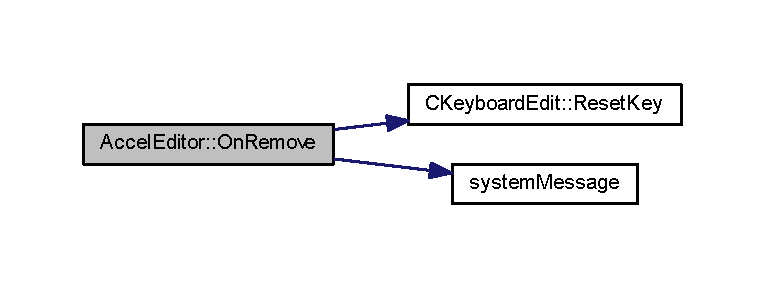
\includegraphics[width=350pt]{class_accel_editor_a40b74b67b95694245502b15ceedd278c_cgraph}
\end{center}
\end{figure}
\mbox{\Hypertarget{class_accel_editor_a1afed0a04125915ae1517e1b08879b8b}\label{class_accel_editor_a1afed0a04125915ae1517e1b08879b8b}} 
\index{Accel\+Editor@{Accel\+Editor}!On\+Reset@{On\+Reset}}
\index{On\+Reset@{On\+Reset}!Accel\+Editor@{Accel\+Editor}}
\subsubsection{\texorpdfstring{On\+Reset()}{OnReset()}}
{\footnotesize\ttfamily void Accel\+Editor\+::\+On\+Reset (\begin{DoxyParamCaption}{ }\end{DoxyParamCaption})\hspace{0.3cm}{\ttfamily [protected]}}



Accel\+Editor.\+cpp 파일의 167 번째 라인에서 정의되었습니다.


\begin{DoxyCode}
168 \{
169   \mbox{\hyperlink{class_accel_editor_acb731e2193cb5022a95e83122651f96d}{mgr}}.\mbox{\hyperlink{class_c_accelerator_manager_aa510a36964ed209de5f7325efa713bf6}{Default}}();
170   \mbox{\hyperlink{class_accel_editor_a3c882fb85c72711e26cfe800fb11ccfa}{InitCommands}}(); \textcolor{comment}{// update the listboxes.}
171 \}
\end{DoxyCode}
이 함수 내부에서 호출하는 함수들에 대한 그래프입니다.\+:
\nopagebreak
\begin{figure}[H]
\begin{center}
\leavevmode
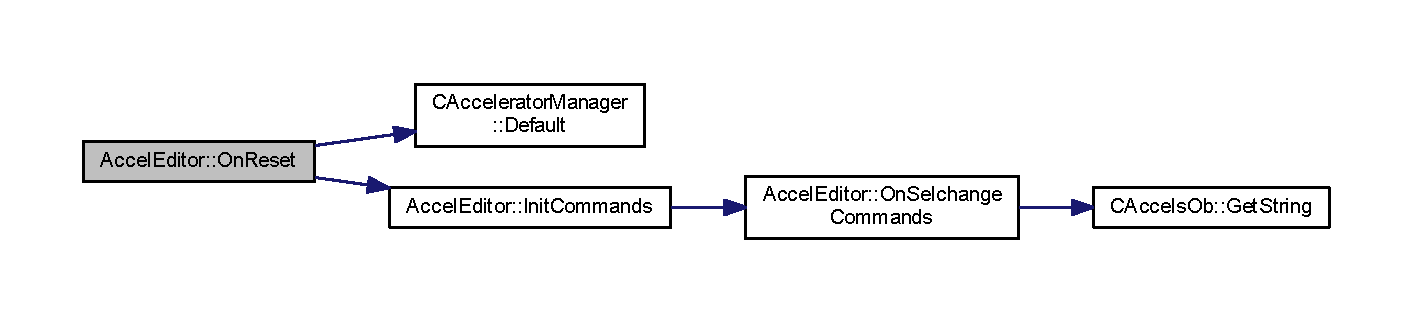
\includegraphics[width=350pt]{class_accel_editor_a1afed0a04125915ae1517e1b08879b8b_cgraph}
\end{center}
\end{figure}
\mbox{\Hypertarget{class_accel_editor_a16cb5c73f55199115c5a4f35268ff3fa}\label{class_accel_editor_a16cb5c73f55199115c5a4f35268ff3fa}} 
\index{Accel\+Editor@{Accel\+Editor}!On\+Selchange\+Commands@{On\+Selchange\+Commands}}
\index{On\+Selchange\+Commands@{On\+Selchange\+Commands}!Accel\+Editor@{Accel\+Editor}}
\subsubsection{\texorpdfstring{On\+Selchange\+Commands()}{OnSelchangeCommands()}}
{\footnotesize\ttfamily void Accel\+Editor\+::\+On\+Selchange\+Commands (\begin{DoxyParamCaption}{ }\end{DoxyParamCaption})\hspace{0.3cm}{\ttfamily [protected]}}



Accel\+Editor.\+cpp 파일의 136 번째 라인에서 정의되었습니다.


\begin{DoxyCode}
137 \{
138   \textcolor{comment}{// Check if some commands exist.}
139   \textcolor{keywordtype}{int} index = \mbox{\hyperlink{class_accel_editor_aba4ea3d3eced08de9fe39e307b5f40fc}{m\_commands}}.GetCurSel();
140   \textcolor{keywordflow}{if} (index == LB\_ERR)
141     \textcolor{keywordflow}{return};
142 
143   WORD wIDCommand = LOWORD(\mbox{\hyperlink{class_accel_editor_aba4ea3d3eced08de9fe39e307b5f40fc}{m\_commands}}.GetItemData(index));
144   \mbox{\hyperlink{class_accel_editor_a31909da8a929ef7b5e22ffbf64f1c68c}{m\_currents}}.ResetContent();
145 
146   \mbox{\hyperlink{class_c_cmd_accel_ob}{CCmdAccelOb}}* pCmdAccel;
147   
148   \textcolor{keywordflow}{if} (\mbox{\hyperlink{class_accel_editor_acb731e2193cb5022a95e83122651f96d}{mgr}}.\mbox{\hyperlink{class_c_accelerator_manager_a16b8d3e9328bc0eeeb048630deff2768}{m\_mapAccelTable}}.Lookup(wIDCommand, pCmdAccel)) \{
149     \mbox{\hyperlink{class_c_accels_ob}{CAccelsOb}}* pAccel;
150     CString szBuffer;
151     POSITION pos = pCmdAccel->\mbox{\hyperlink{class_c_cmd_accel_ob_a85772f1ea9204af42b8a39a0135dc0f8}{m\_Accels}}.GetHeadPosition();
152 
153     \textcolor{comment}{// Add the keys to the 'currents keys' listbox.}
154     \textcolor{keywordflow}{while} (pos != \mbox{\hyperlink{getopt1_8c_a070d2ce7b6bb7e5c05602aa8c308d0c4}{NULL}}) \{
155       pAccel = pCmdAccel->\mbox{\hyperlink{class_c_cmd_accel_ob_a85772f1ea9204af42b8a39a0135dc0f8}{m\_Accels}}.GetNext(pos);
156       pAccel->\mbox{\hyperlink{class_c_accels_ob_afaf7510fa1e0707863f6bd469f190de6}{GetString}}(szBuffer);
157       index = \mbox{\hyperlink{class_accel_editor_a31909da8a929ef7b5e22ffbf64f1c68c}{m\_currents}}.AddString(szBuffer);
158       \textcolor{comment}{// and a pointer to the accel object.}
159       \mbox{\hyperlink{class_accel_editor_a31909da8a929ef7b5e22ffbf64f1c68c}{m\_currents}}.SetItemData(index, (DWORD\_PTR)pAccel);
160     \}
161   \}
162   \textcolor{comment}{// Init the key editor}
163   \textcolor{comment}{//  m\_pKey->ResetKey();}
164 
165 \}
\end{DoxyCode}
이 함수 내부에서 호출하는 함수들에 대한 그래프입니다.\+:
\nopagebreak
\begin{figure}[H]
\begin{center}
\leavevmode
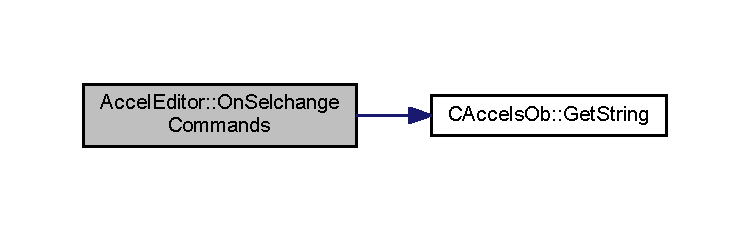
\includegraphics[width=350pt]{class_accel_editor_a16cb5c73f55199115c5a4f35268ff3fa_cgraph}
\end{center}
\end{figure}
이 함수를 호출하는 함수들에 대한 그래프입니다.\+:
\nopagebreak
\begin{figure}[H]
\begin{center}
\leavevmode
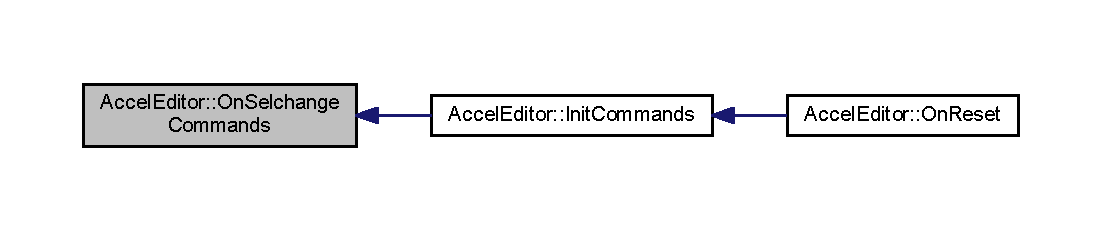
\includegraphics[width=350pt]{class_accel_editor_a16cb5c73f55199115c5a4f35268ff3fa_icgraph}
\end{center}
\end{figure}


\subsection{멤버 데이터 문서화}
\mbox{\Hypertarget{class_accel_editor_ac3d2378be850611ee51689bd34475275}\label{class_accel_editor_ac3d2378be850611ee51689bd34475275}} 
\index{Accel\+Editor@{Accel\+Editor}!m\+\_\+already\+Affected@{m\+\_\+already\+Affected}}
\index{m\+\_\+already\+Affected@{m\+\_\+already\+Affected}!Accel\+Editor@{Accel\+Editor}}
\subsubsection{\texorpdfstring{m\+\_\+already\+Affected}{m\_alreadyAffected}}
{\footnotesize\ttfamily C\+Static Accel\+Editor\+::m\+\_\+already\+Affected}



Accel\+Editor.\+h 파일의 47 번째 라인에서 정의되었습니다.

\mbox{\Hypertarget{class_accel_editor_aba4ea3d3eced08de9fe39e307b5f40fc}\label{class_accel_editor_aba4ea3d3eced08de9fe39e307b5f40fc}} 
\index{Accel\+Editor@{Accel\+Editor}!m\+\_\+commands@{m\+\_\+commands}}
\index{m\+\_\+commands@{m\+\_\+commands}!Accel\+Editor@{Accel\+Editor}}
\subsubsection{\texorpdfstring{m\+\_\+commands}{m\_commands}}
{\footnotesize\ttfamily C\+List\+Box Accel\+Editor\+::m\+\_\+commands}



Accel\+Editor.\+h 파일의 48 번째 라인에서 정의되었습니다.

\mbox{\Hypertarget{class_accel_editor_a31909da8a929ef7b5e22ffbf64f1c68c}\label{class_accel_editor_a31909da8a929ef7b5e22ffbf64f1c68c}} 
\index{Accel\+Editor@{Accel\+Editor}!m\+\_\+currents@{m\+\_\+currents}}
\index{m\+\_\+currents@{m\+\_\+currents}!Accel\+Editor@{Accel\+Editor}}
\subsubsection{\texorpdfstring{m\+\_\+currents}{m\_currents}}
{\footnotesize\ttfamily C\+List\+Box Accel\+Editor\+::m\+\_\+currents}



Accel\+Editor.\+h 파일의 46 번째 라인에서 정의되었습니다.

\mbox{\Hypertarget{class_accel_editor_af0875f914fdddf5233a951cabd499a4d}\label{class_accel_editor_af0875f914fdddf5233a951cabd499a4d}} 
\index{Accel\+Editor@{Accel\+Editor}!m\+\_\+key@{m\+\_\+key}}
\index{m\+\_\+key@{m\+\_\+key}!Accel\+Editor@{Accel\+Editor}}
\subsubsection{\texorpdfstring{m\+\_\+key}{m\_key}}
{\footnotesize\ttfamily \mbox{\hyperlink{class_c_keyboard_edit}{C\+Keyboard\+Edit}} Accel\+Editor\+::m\+\_\+key}



Accel\+Editor.\+h 파일의 49 번째 라인에서 정의되었습니다.

\mbox{\Hypertarget{class_accel_editor_acb731e2193cb5022a95e83122651f96d}\label{class_accel_editor_acb731e2193cb5022a95e83122651f96d}} 
\index{Accel\+Editor@{Accel\+Editor}!mgr@{mgr}}
\index{mgr@{mgr}!Accel\+Editor@{Accel\+Editor}}
\subsubsection{\texorpdfstring{mgr}{mgr}}
{\footnotesize\ttfamily \mbox{\hyperlink{class_c_accelerator_manager}{C\+Accelerator\+Manager}} Accel\+Editor\+::mgr}



Accel\+Editor.\+h 파일의 39 번째 라인에서 정의되었습니다.



이 클래스에 대한 문서화 페이지는 다음의 파일들로부터 생성되었습니다.\+:\begin{DoxyCompactItemize}
\item 
C\+:/\+Users/sjh13/sources/\+Visual\+Boy\+Advance/src/win32/\mbox{\hyperlink{_accel_editor_8h}{Accel\+Editor.\+h}}\item 
C\+:/\+Users/sjh13/sources/\+Visual\+Boy\+Advance/src/win32/\mbox{\hyperlink{_accel_editor_8cpp}{Accel\+Editor.\+cpp}}\end{DoxyCompactItemize}

\hypertarget{class_add_c_b_a_code}{}\section{Add\+C\+B\+A\+Code 클래스 참조}
\label{class_add_c_b_a_code}\index{Add\+C\+B\+A\+Code@{Add\+C\+B\+A\+Code}}


{\ttfamily \#include $<$G\+B\+A\+Cheats.\+h$>$}



Add\+C\+B\+A\+Code에 대한 상속 다이어그램 \+: \nopagebreak
\begin{figure}[H]
\begin{center}
\leavevmode
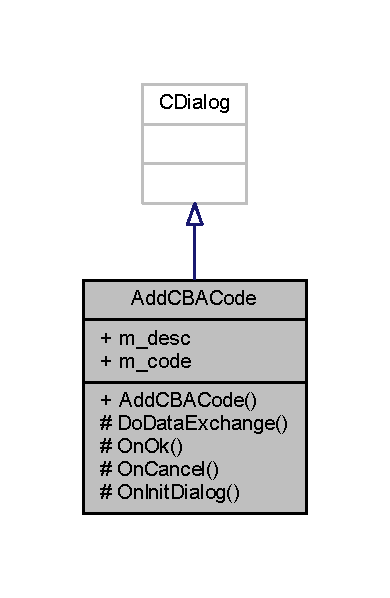
\includegraphics[width=187pt]{class_add_c_b_a_code__inherit__graph}
\end{center}
\end{figure}


Add\+C\+B\+A\+Code에 대한 협력 다이어그램\+:\nopagebreak
\begin{figure}[H]
\begin{center}
\leavevmode
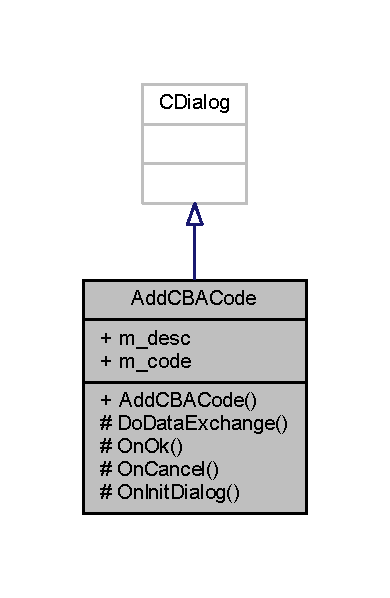
\includegraphics[width=187pt]{class_add_c_b_a_code__coll__graph}
\end{center}
\end{figure}
\subsection*{Public 타입}
\begin{DoxyCompactItemize}
\item 
enum \{ \mbox{\hyperlink{class_add_c_b_a_code_ab086df2c41fbfe55405c6ac046dab7a5a74bfcc1c249905cacf32559b0a875855}{I\+DD}} = I\+D\+D\+\_\+\+A\+D\+D\+\_\+\+C\+H\+E\+A\+T\+\_\+\+D\+LG
 \}
\end{DoxyCompactItemize}
\subsection*{Public 멤버 함수}
\begin{DoxyCompactItemize}
\item 
\mbox{\hyperlink{class_add_c_b_a_code_a13fcdd2e1451c66ac0744a631d95fdb8}{Add\+C\+B\+A\+Code}} (C\+Wnd $\ast$p\+Parent=\mbox{\hyperlink{_system_8h_a070d2ce7b6bb7e5c05602aa8c308d0c4}{N\+U\+LL}})
\end{DoxyCompactItemize}
\subsection*{Public 속성}
\begin{DoxyCompactItemize}
\item 
C\+Edit \mbox{\hyperlink{class_add_c_b_a_code_ab5056f88f9c1f58a20a1ce718599305b}{m\+\_\+desc}}
\item 
C\+Edit \mbox{\hyperlink{class_add_c_b_a_code_ab4b404e9aed23e5dd265f543e98c9c6c}{m\+\_\+code}}
\end{DoxyCompactItemize}
\subsection*{Protected 멤버 함수}
\begin{DoxyCompactItemize}
\item 
virtual void \mbox{\hyperlink{class_add_c_b_a_code_a62f9304a8dd24bfd4621e59ba5073cc4}{Do\+Data\+Exchange}} (C\+Data\+Exchange $\ast$p\+DX)
\item 
afx\+\_\+msg void \mbox{\hyperlink{class_add_c_b_a_code_a63c5cc95366a1a0aad123432054f977a}{On\+Ok}} ()
\item 
afx\+\_\+msg void \mbox{\hyperlink{class_add_c_b_a_code_a94c94b1c124bb028f9237ee9bfa9f41d}{On\+Cancel}} ()
\item 
virtual B\+O\+OL \mbox{\hyperlink{class_add_c_b_a_code_a302c75c08dacdd95eecff6b3b74ebbe6}{On\+Init\+Dialog}} ()
\end{DoxyCompactItemize}


\subsection{상세한 설명}


G\+B\+A\+Cheats.\+h 파일의 220 번째 라인에서 정의되었습니다.



\subsection{멤버 열거형 문서화}
\mbox{\Hypertarget{class_add_c_b_a_code_ab086df2c41fbfe55405c6ac046dab7a5}\label{class_add_c_b_a_code_ab086df2c41fbfe55405c6ac046dab7a5}} 
\subsubsection{\texorpdfstring{anonymous enum}{anonymous enum}}
{\footnotesize\ttfamily anonymous enum}

\begin{DoxyEnumFields}{열거형 멤버}
\raisebox{\heightof{T}}[0pt][0pt]{\index{I\+DD@{I\+DD}!Add\+C\+B\+A\+Code@{Add\+C\+B\+A\+Code}}\index{Add\+C\+B\+A\+Code@{Add\+C\+B\+A\+Code}!I\+DD@{I\+DD}}}\mbox{\Hypertarget{class_add_c_b_a_code_ab086df2c41fbfe55405c6ac046dab7a5a74bfcc1c249905cacf32559b0a875855}\label{class_add_c_b_a_code_ab086df2c41fbfe55405c6ac046dab7a5a74bfcc1c249905cacf32559b0a875855}} 
I\+DD&\\
\hline

\end{DoxyEnumFields}


G\+B\+A\+Cheats.\+h 파일의 228 번째 라인에서 정의되었습니다.


\begin{DoxyCode}
228 \{ \mbox{\hyperlink{class_add_c_b_a_code_ab086df2c41fbfe55405c6ac046dab7a5a74bfcc1c249905cacf32559b0a875855}{IDD}} = \mbox{\hyperlink{resource_8h_a388a8d7b6dea32798ece69044a21790d}{IDD\_ADD\_CHEAT\_DLG}} \};
\end{DoxyCode}


\subsection{생성자 \& 소멸자 문서화}
\mbox{\Hypertarget{class_add_c_b_a_code_a13fcdd2e1451c66ac0744a631d95fdb8}\label{class_add_c_b_a_code_a13fcdd2e1451c66ac0744a631d95fdb8}} 
\index{Add\+C\+B\+A\+Code@{Add\+C\+B\+A\+Code}!Add\+C\+B\+A\+Code@{Add\+C\+B\+A\+Code}}
\index{Add\+C\+B\+A\+Code@{Add\+C\+B\+A\+Code}!Add\+C\+B\+A\+Code@{Add\+C\+B\+A\+Code}}
\subsubsection{\texorpdfstring{Add\+C\+B\+A\+Code()}{AddCBACode()}}
{\footnotesize\ttfamily Add\+C\+B\+A\+Code\+::\+Add\+C\+B\+A\+Code (\begin{DoxyParamCaption}\item[{C\+Wnd $\ast$}]{p\+Parent = {\ttfamily \mbox{\hyperlink{_system_8h_a070d2ce7b6bb7e5c05602aa8c308d0c4}{N\+U\+LL}}} }\end{DoxyParamCaption})}



G\+B\+A\+Cheats.\+cpp 파일의 1010 번째 라인에서 정의되었습니다.


\begin{DoxyCode}
1011   : CDialog(\mbox{\hyperlink{class_add_c_b_a_code_ab086df2c41fbfe55405c6ac046dab7a5a74bfcc1c249905cacf32559b0a875855}{AddCBACode::IDD}}, pParent)
1012 \{
1013   \textcolor{comment}{//\{\{AFX\_DATA\_INIT(AddCBACode)}
1014   \textcolor{comment}{// NOTE: the ClassWizard will add member initialization here}
1015   \textcolor{comment}{//\}\}AFX\_DATA\_INIT}
1016 \}
\end{DoxyCode}


\subsection{멤버 함수 문서화}
\mbox{\Hypertarget{class_add_c_b_a_code_a62f9304a8dd24bfd4621e59ba5073cc4}\label{class_add_c_b_a_code_a62f9304a8dd24bfd4621e59ba5073cc4}} 
\index{Add\+C\+B\+A\+Code@{Add\+C\+B\+A\+Code}!Do\+Data\+Exchange@{Do\+Data\+Exchange}}
\index{Do\+Data\+Exchange@{Do\+Data\+Exchange}!Add\+C\+B\+A\+Code@{Add\+C\+B\+A\+Code}}
\subsubsection{\texorpdfstring{Do\+Data\+Exchange()}{DoDataExchange()}}
{\footnotesize\ttfamily void Add\+C\+B\+A\+Code\+::\+Do\+Data\+Exchange (\begin{DoxyParamCaption}\item[{C\+Data\+Exchange $\ast$}]{p\+DX }\end{DoxyParamCaption})\hspace{0.3cm}{\ttfamily [protected]}, {\ttfamily [virtual]}}



G\+B\+A\+Cheats.\+cpp 파일의 1019 번째 라인에서 정의되었습니다.


\begin{DoxyCode}
1020 \{
1021   CDialog::DoDataExchange(pDX);
1022   \textcolor{comment}{//\{\{AFX\_DATA\_MAP(AddCBACode)}
1023   DDX\_Control(pDX, \mbox{\hyperlink{resource_8h_adb05cf1e74135587a9b3ab93a5152feb}{IDC\_DESC}}, \mbox{\hyperlink{class_add_c_b_a_code_ab5056f88f9c1f58a20a1ce718599305b}{m\_desc}});
1024   DDX\_Control(pDX, \mbox{\hyperlink{resource_8h_abb149f0043fd3834639ddb2d80d31723}{IDC\_CODE}}, \mbox{\hyperlink{class_add_c_b_a_code_ab4b404e9aed23e5dd265f543e98c9c6c}{m\_code}});
1025   \textcolor{comment}{//\}\}AFX\_DATA\_MAP}
1026 \}
\end{DoxyCode}
\mbox{\Hypertarget{class_add_c_b_a_code_a94c94b1c124bb028f9237ee9bfa9f41d}\label{class_add_c_b_a_code_a94c94b1c124bb028f9237ee9bfa9f41d}} 
\index{Add\+C\+B\+A\+Code@{Add\+C\+B\+A\+Code}!On\+Cancel@{On\+Cancel}}
\index{On\+Cancel@{On\+Cancel}!Add\+C\+B\+A\+Code@{Add\+C\+B\+A\+Code}}
\subsubsection{\texorpdfstring{On\+Cancel()}{OnCancel()}}
{\footnotesize\ttfamily void Add\+C\+B\+A\+Code\+::\+On\+Cancel (\begin{DoxyParamCaption}{ }\end{DoxyParamCaption})\hspace{0.3cm}{\ttfamily [protected]}}



G\+B\+A\+Cheats.\+cpp 파일의 1083 번째 라인에서 정의되었습니다.


\begin{DoxyCode}
1084 \{
1085   EndDialog(FALSE);
1086 \}
\end{DoxyCode}
\mbox{\Hypertarget{class_add_c_b_a_code_a302c75c08dacdd95eecff6b3b74ebbe6}\label{class_add_c_b_a_code_a302c75c08dacdd95eecff6b3b74ebbe6}} 
\index{Add\+C\+B\+A\+Code@{Add\+C\+B\+A\+Code}!On\+Init\+Dialog@{On\+Init\+Dialog}}
\index{On\+Init\+Dialog@{On\+Init\+Dialog}!Add\+C\+B\+A\+Code@{Add\+C\+B\+A\+Code}}
\subsubsection{\texorpdfstring{On\+Init\+Dialog()}{OnInitDialog()}}
{\footnotesize\ttfamily B\+O\+OL Add\+C\+B\+A\+Code\+::\+On\+Init\+Dialog (\begin{DoxyParamCaption}{ }\end{DoxyParamCaption})\hspace{0.3cm}{\ttfamily [protected]}, {\ttfamily [virtual]}}



G\+B\+A\+Cheats.\+cpp 파일의 1088 번째 라인에서 정의되었습니다.


\begin{DoxyCode}
1089 \{
1090   CDialog::OnInitDialog();
1091   
1092   \mbox{\hyperlink{class_add_c_b_a_code_ab4b404e9aed23e5dd265f543e98c9c6c}{m\_code}}.LimitText(1024);
1093   \mbox{\hyperlink{class_add_c_b_a_code_ab5056f88f9c1f58a20a1ce718599305b}{m\_desc}}.LimitText(32);
1094   CString title = \mbox{\hyperlink{_win_res_util_8cpp_a416e85e80ab9b01376e87251c83d1a5a}{winResLoadString}}(\mbox{\hyperlink{resource_8h_add1ed8080a9328ce15770b3f9bd29b09}{IDS\_ADD\_CBA\_CODE}});
1095   SetWindowText(title);
1096   CenterWindow();
1097   
1098   \textcolor{keywordflow}{return} TRUE;  \textcolor{comment}{// return TRUE unless you set the focus to a control}
1099                 \textcolor{comment}{// EXCEPTION: OCX Property Pages should return FALSE}
1100 \}
\end{DoxyCode}
이 함수 내부에서 호출하는 함수들에 대한 그래프입니다.\+:
\nopagebreak
\begin{figure}[H]
\begin{center}
\leavevmode
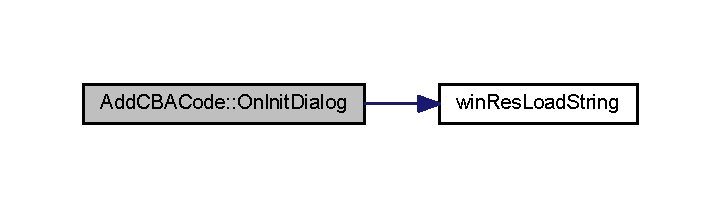
\includegraphics[width=346pt]{class_add_c_b_a_code_a302c75c08dacdd95eecff6b3b74ebbe6_cgraph}
\end{center}
\end{figure}
\mbox{\Hypertarget{class_add_c_b_a_code_a63c5cc95366a1a0aad123432054f977a}\label{class_add_c_b_a_code_a63c5cc95366a1a0aad123432054f977a}} 
\index{Add\+C\+B\+A\+Code@{Add\+C\+B\+A\+Code}!On\+Ok@{On\+Ok}}
\index{On\+Ok@{On\+Ok}!Add\+C\+B\+A\+Code@{Add\+C\+B\+A\+Code}}
\subsubsection{\texorpdfstring{On\+Ok()}{OnOk()}}
{\footnotesize\ttfamily void Add\+C\+B\+A\+Code\+::\+On\+Ok (\begin{DoxyParamCaption}{ }\end{DoxyParamCaption})\hspace{0.3cm}{\ttfamily [protected]}}



G\+B\+A\+Cheats.\+cpp 파일의 1039 번째 라인에서 정의되었습니다.


\begin{DoxyCode}
1040 \{
1041   CString desc;
1042   CString \mbox{\hyperlink{_g_b_a_8cpp_a28d4d3d8445e73a696b2d6f7eadabd96}{buffer}};
1043   CString part1;
1044   CString code;
1045   CString token;
1046 
1047   \mbox{\hyperlink{class_add_c_b_a_code_ab4b404e9aed23e5dd265f543e98c9c6c}{m\_code}}.GetWindowText(\mbox{\hyperlink{_g_b_a_8cpp_a28d4d3d8445e73a696b2d6f7eadabd96}{buffer}});
1048   \mbox{\hyperlink{class_add_c_b_a_code_ab5056f88f9c1f58a20a1ce718599305b}{m\_desc}}.GetWindowText(desc);
1049   
1050   \mbox{\hyperlink{class_string_tokenizer}{StringTokenizer}} st(\mbox{\hyperlink{_g_b_a_8cpp_a28d4d3d8445e73a696b2d6f7eadabd96}{buffer}}, \textcolor{stringliteral}{" \(\backslash\)t\(\backslash\)n\(\backslash\)r"});
1051   part1.Empty();
1052   \textcolor{keyword}{const} \textcolor{keywordtype}{char} *\mbox{\hyperlink{expr_8cpp_aded116371789db1fd63c90ef00c95a3d}{t}} = st.next();
1053   \textcolor{keywordflow}{while}(\mbox{\hyperlink{expr_8cpp_aded116371789db1fd63c90ef00c95a3d}{t}}) \{
1054     token = \mbox{\hyperlink{expr_8cpp_aded116371789db1fd63c90ef00c95a3d}{t}};
1055     token.MakeUpper();
1056     \textcolor{keywordflow}{if}(token.GetLength() == 16)
1057       \mbox{\hyperlink{_cheats_8cpp_a47aded7deffcbfa36ed55944eafb72ab}{cheatsAddGSACode}}(token, desc, \textcolor{keyword}{false});
1058     \textcolor{keywordflow}{else} \textcolor{keywordflow}{if}(token.GetLength() == 12) \{
1059       code = token.Left(8);
1060       code += \textcolor{stringliteral}{" "};
1061       code += token.Right(4);
1062       \mbox{\hyperlink{_cheats_8cpp_af79d349aaea63793beec4fa2626f74c8}{cheatsAddCBACode}}(code, desc);
1063     \} \textcolor{keywordflow}{else} \textcolor{keywordflow}{if}(part1.IsEmpty())
1064       part1 = token;
1065     \textcolor{keywordflow}{else} \{
1066       \textcolor{keywordflow}{if}(token.GetLength() == 4) \{
1067         code = part1;
1068         code += \textcolor{stringliteral}{" "};
1069         code += token;
1070         \mbox{\hyperlink{_cheats_8cpp_af79d349aaea63793beec4fa2626f74c8}{cheatsAddCBACode}}(code, desc);
1071       \} \textcolor{keywordflow}{else} \{
1072         code = part1 + token;
1073         \mbox{\hyperlink{_cheats_8cpp_a47aded7deffcbfa36ed55944eafb72ab}{cheatsAddGSACode}}(code, desc, \textcolor{keyword}{true});
1074       \}
1075       part1.Empty();
1076     \}
1077 
1078     \mbox{\hyperlink{expr_8cpp_aded116371789db1fd63c90ef00c95a3d}{t}} = st.next();
1079   \}
1080   EndDialog(TRUE);
1081 \}
\end{DoxyCode}
이 함수 내부에서 호출하는 함수들에 대한 그래프입니다.\+:
\nopagebreak
\begin{figure}[H]
\begin{center}
\leavevmode
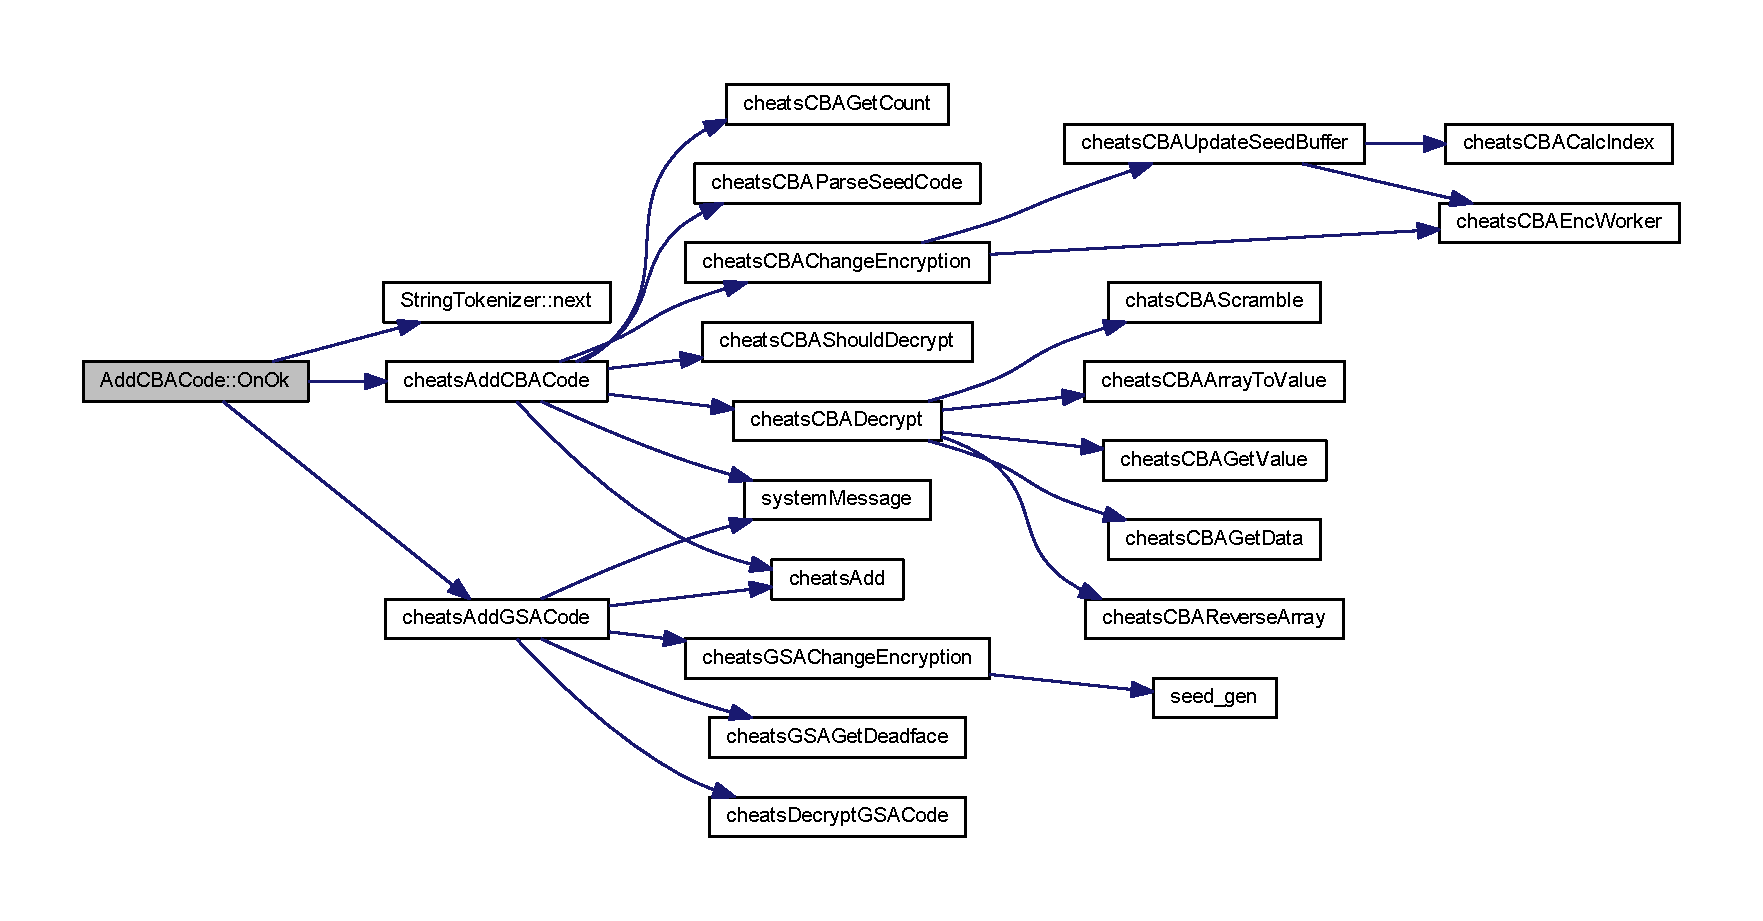
\includegraphics[width=350pt]{class_add_c_b_a_code_a63c5cc95366a1a0aad123432054f977a_cgraph}
\end{center}
\end{figure}


\subsection{멤버 데이터 문서화}
\mbox{\Hypertarget{class_add_c_b_a_code_ab4b404e9aed23e5dd265f543e98c9c6c}\label{class_add_c_b_a_code_ab4b404e9aed23e5dd265f543e98c9c6c}} 
\index{Add\+C\+B\+A\+Code@{Add\+C\+B\+A\+Code}!m\+\_\+code@{m\+\_\+code}}
\index{m\+\_\+code@{m\+\_\+code}!Add\+C\+B\+A\+Code@{Add\+C\+B\+A\+Code}}
\subsubsection{\texorpdfstring{m\+\_\+code}{m\_code}}
{\footnotesize\ttfamily C\+Edit Add\+C\+B\+A\+Code\+::m\+\_\+code}



G\+B\+A\+Cheats.\+h 파일의 230 번째 라인에서 정의되었습니다.

\mbox{\Hypertarget{class_add_c_b_a_code_ab5056f88f9c1f58a20a1ce718599305b}\label{class_add_c_b_a_code_ab5056f88f9c1f58a20a1ce718599305b}} 
\index{Add\+C\+B\+A\+Code@{Add\+C\+B\+A\+Code}!m\+\_\+desc@{m\+\_\+desc}}
\index{m\+\_\+desc@{m\+\_\+desc}!Add\+C\+B\+A\+Code@{Add\+C\+B\+A\+Code}}
\subsubsection{\texorpdfstring{m\+\_\+desc}{m\_desc}}
{\footnotesize\ttfamily C\+Edit Add\+C\+B\+A\+Code\+::m\+\_\+desc}



G\+B\+A\+Cheats.\+h 파일의 229 번째 라인에서 정의되었습니다.



이 클래스에 대한 문서화 페이지는 다음의 파일들로부터 생성되었습니다.\+:\begin{DoxyCompactItemize}
\item 
C\+:/\+Users/sjh13/sources/\+Visual\+Boy\+Advance/src/win32/\mbox{\hyperlink{_g_b_a_cheats_8h}{G\+B\+A\+Cheats.\+h}}\item 
C\+:/\+Users/sjh13/sources/\+Visual\+Boy\+Advance/src/win32/\mbox{\hyperlink{_g_b_a_cheats_8cpp}{G\+B\+A\+Cheats.\+cpp}}\end{DoxyCompactItemize}

\hypertarget{class_add_cheat}{}\section{Add\+Cheat 클래스 참조}
\label{class_add_cheat}\index{Add\+Cheat@{Add\+Cheat}}
Add\+Cheat에 대한 상속 다이어그램 \+: \begin{figure}[H]
\begin{center}
\leavevmode
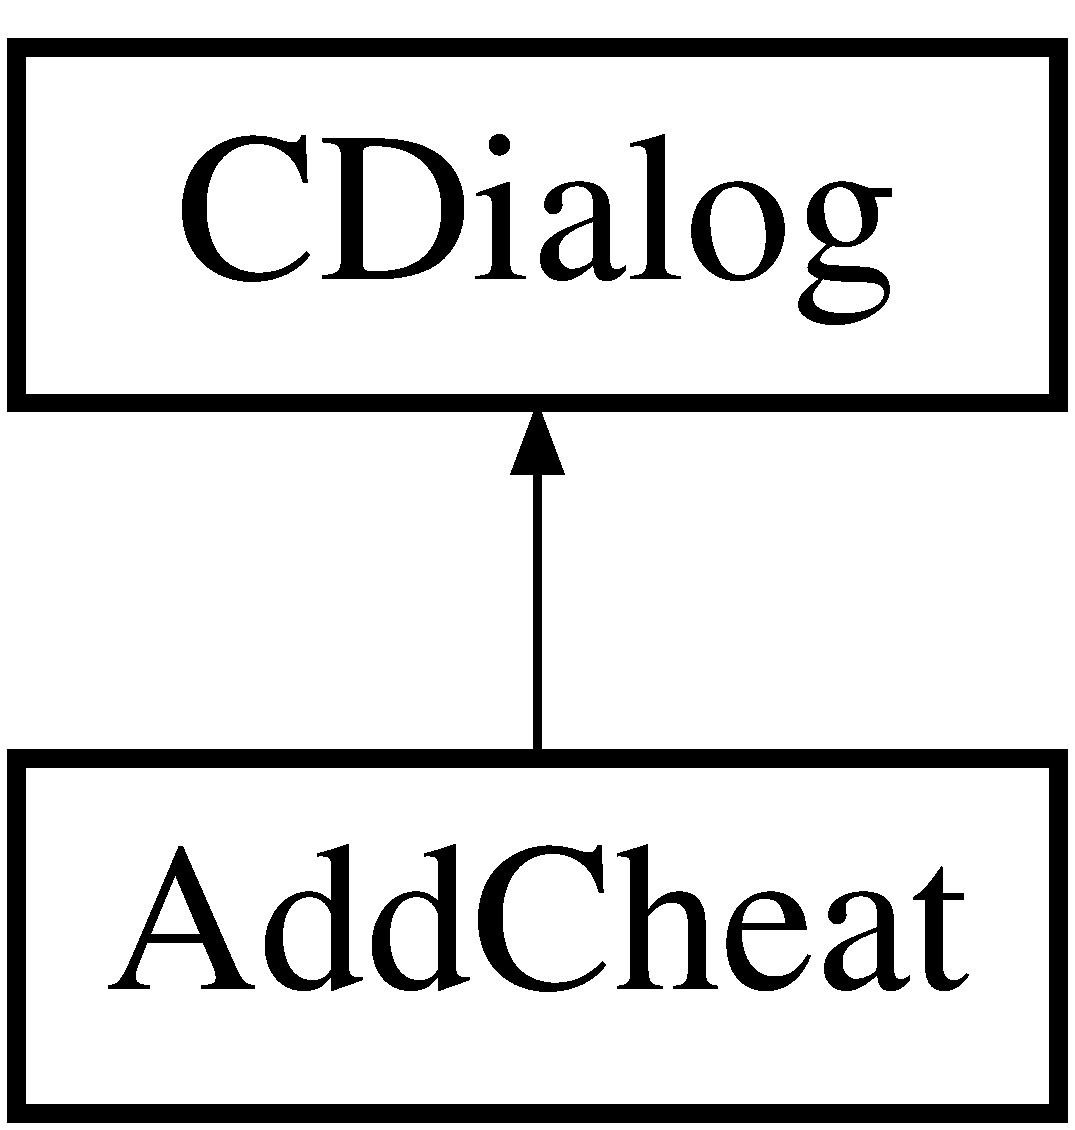
\includegraphics[height=2.000000cm]{class_add_cheat}
\end{center}
\end{figure}
\subsection*{Public 타입}
\begin{DoxyCompactItemize}
\item 
\mbox{\Hypertarget{class_add_cheat_af696833b823db49de5667fcb42b11a26}\label{class_add_cheat_af696833b823db49de5667fcb42b11a26}} 
enum \{ {\bfseries I\+DD} = I\+D\+D\+\_\+\+A\+D\+D\+\_\+\+C\+H\+E\+AT
 \}
\end{DoxyCompactItemize}
\subsection*{Public 멤버 함수}
\begin{DoxyCompactItemize}
\item 
\mbox{\Hypertarget{class_add_cheat_a53989b2f3f179185384d258c9e71ace7}\label{class_add_cheat_a53989b2f3f179185384d258c9e71ace7}} 
bool {\bfseries add\+Cheat} ()
\item 
\mbox{\Hypertarget{class_add_cheat_ae9762fec683ccd9972d29fec47eecba4}\label{class_add_cheat_ae9762fec683ccd9972d29fec47eecba4}} 
afx\+\_\+msg void {\bfseries On\+Size\+Type} (U\+I\+NT id)
\item 
\mbox{\Hypertarget{class_add_cheat_a3ac4c44d5f9ec5037e92034789c276b4}\label{class_add_cheat_a3ac4c44d5f9ec5037e92034789c276b4}} 
afx\+\_\+msg void {\bfseries On\+Number\+Type} (U\+I\+NT id)
\item 
\mbox{\Hypertarget{class_add_cheat_afa75eefc22d2f9449cf3b9283926408c}\label{class_add_cheat_afa75eefc22d2f9449cf3b9283926408c}} 
{\bfseries Add\+Cheat} (u32 address, C\+Wnd $\ast$p\+Parent=N\+U\+LL)
\end{DoxyCompactItemize}
\subsection*{Public 속성}
\begin{DoxyCompactItemize}
\item 
\mbox{\Hypertarget{class_add_cheat_ae21ae20b0a2e3b936b9ecbacb13a2751}\label{class_add_cheat_ae21ae20b0a2e3b936b9ecbacb13a2751}} 
u32 {\bfseries address}
\item 
\mbox{\Hypertarget{class_add_cheat_aff9c3fd61a088f03dba1eb01e6956286}\label{class_add_cheat_aff9c3fd61a088f03dba1eb01e6956286}} 
C\+Edit {\bfseries m\+\_\+value}
\item 
\mbox{\Hypertarget{class_add_cheat_a644f29b6dd8a0d26d5050054bdf2b054}\label{class_add_cheat_a644f29b6dd8a0d26d5050054bdf2b054}} 
C\+Edit {\bfseries m\+\_\+desc}
\item 
\mbox{\Hypertarget{class_add_cheat_a27ec0f498f3827cfc81c19d963c7fef5}\label{class_add_cheat_a27ec0f498f3827cfc81c19d963c7fef5}} 
C\+Edit {\bfseries m\+\_\+address}
\item 
\mbox{\Hypertarget{class_add_cheat_a7c3af367e51b1812d951dd2d24ac1aa8}\label{class_add_cheat_a7c3af367e51b1812d951dd2d24ac1aa8}} 
int {\bfseries size\+Type}
\item 
\mbox{\Hypertarget{class_add_cheat_a50115e7ad42a106db574754cc81bc9a0}\label{class_add_cheat_a50115e7ad42a106db574754cc81bc9a0}} 
int {\bfseries number\+Type}
\end{DoxyCompactItemize}
\subsection*{Protected 멤버 함수}
\begin{DoxyCompactItemize}
\item 
\mbox{\Hypertarget{class_add_cheat_a9d3dbf5955873700caf71f41fa5117cc}\label{class_add_cheat_a9d3dbf5955873700caf71f41fa5117cc}} 
virtual void {\bfseries Do\+Data\+Exchange} (C\+Data\+Exchange $\ast$p\+DX)
\item 
\mbox{\Hypertarget{class_add_cheat_ad3785b90d963668a87ff33fb93cf56d9}\label{class_add_cheat_ad3785b90d963668a87ff33fb93cf56d9}} 
afx\+\_\+msg void {\bfseries On\+Ok} ()
\item 
\mbox{\Hypertarget{class_add_cheat_aef14a7fa535621c242e9007a7c0510e7}\label{class_add_cheat_aef14a7fa535621c242e9007a7c0510e7}} 
afx\+\_\+msg void {\bfseries On\+Cancel} ()
\item 
\mbox{\Hypertarget{class_add_cheat_a92017eb0efe50e09e7c3e5e4980a18cb}\label{class_add_cheat_a92017eb0efe50e09e7c3e5e4980a18cb}} 
virtual B\+O\+OL {\bfseries On\+Init\+Dialog} ()
\end{DoxyCompactItemize}


이 클래스에 대한 문서화 페이지는 다음의 파일들로부터 생성되었습니다.\+:\begin{DoxyCompactItemize}
\item 
src/win32/G\+B\+A\+Cheats.\+h\item 
src/win32/G\+B\+A\+Cheats.\+cpp\end{DoxyCompactItemize}

\hypertarget{class_add_cheat_code}{}\section{Add\+Cheat\+Code 클래스 참조}
\label{class_add_cheat_code}\index{Add\+Cheat\+Code@{Add\+Cheat\+Code}}


{\ttfamily \#include $<$G\+B\+A\+Cheats.\+h$>$}



Add\+Cheat\+Code에 대한 상속 다이어그램 \+: \nopagebreak
\begin{figure}[H]
\begin{center}
\leavevmode
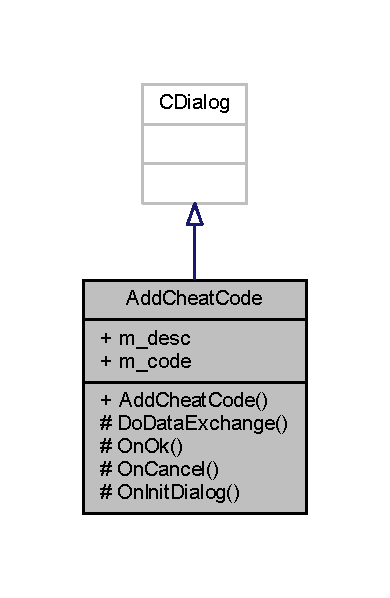
\includegraphics[width=187pt]{class_add_cheat_code__inherit__graph}
\end{center}
\end{figure}


Add\+Cheat\+Code에 대한 협력 다이어그램\+:\nopagebreak
\begin{figure}[H]
\begin{center}
\leavevmode
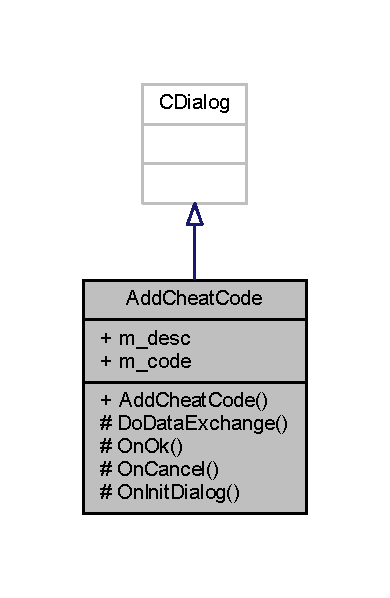
\includegraphics[width=187pt]{class_add_cheat_code__coll__graph}
\end{center}
\end{figure}
\subsection*{Public 타입}
\begin{DoxyCompactItemize}
\item 
enum \{ \mbox{\hyperlink{class_add_cheat_code_a360bc0f5ed2a9d0598c246993ecb57c2a7065caea1931a69dc54b0161b9295ba9}{I\+DD}} = I\+D\+D\+\_\+\+A\+D\+D\+\_\+\+C\+H\+E\+A\+T\+\_\+\+D\+LG
 \}
\end{DoxyCompactItemize}
\subsection*{Public 멤버 함수}
\begin{DoxyCompactItemize}
\item 
\mbox{\hyperlink{class_add_cheat_code_a6904f72f50b5354c479d73ea19dba1ab}{Add\+Cheat\+Code}} (C\+Wnd $\ast$p\+Parent=\mbox{\hyperlink{_system_8h_a070d2ce7b6bb7e5c05602aa8c308d0c4}{N\+U\+LL}})
\end{DoxyCompactItemize}
\subsection*{Public 속성}
\begin{DoxyCompactItemize}
\item 
C\+Edit \mbox{\hyperlink{class_add_cheat_code_a5bbe6b54e71db26da7b3abc7449b3342}{m\+\_\+desc}}
\item 
C\+Edit \mbox{\hyperlink{class_add_cheat_code_a9ae1d05acf10bc6fc8ea8cce2ec2cc6a}{m\+\_\+code}}
\end{DoxyCompactItemize}
\subsection*{Protected 멤버 함수}
\begin{DoxyCompactItemize}
\item 
virtual void \mbox{\hyperlink{class_add_cheat_code_af260d01bd5166f11c1e92894e36c7ad6}{Do\+Data\+Exchange}} (C\+Data\+Exchange $\ast$p\+DX)
\item 
afx\+\_\+msg void \mbox{\hyperlink{class_add_cheat_code_a77b1ec1f5e067495aef92a2f9b8750c8}{On\+Ok}} ()
\item 
afx\+\_\+msg void \mbox{\hyperlink{class_add_cheat_code_abbf22fde6ad9aa52439e4cb4a3d8418b}{On\+Cancel}} ()
\item 
virtual B\+O\+OL \mbox{\hyperlink{class_add_cheat_code_a7818441d921e63c1b0983e86b60beeba}{On\+Init\+Dialog}} ()
\end{DoxyCompactItemize}


\subsection{상세한 설명}


G\+B\+A\+Cheats.\+h 파일의 256 번째 라인에서 정의되었습니다.



\subsection{멤버 열거형 문서화}
\mbox{\Hypertarget{class_add_cheat_code_a360bc0f5ed2a9d0598c246993ecb57c2}\label{class_add_cheat_code_a360bc0f5ed2a9d0598c246993ecb57c2}} 
\subsubsection{\texorpdfstring{anonymous enum}{anonymous enum}}
{\footnotesize\ttfamily anonymous enum}

\begin{DoxyEnumFields}{열거형 멤버}
\raisebox{\heightof{T}}[0pt][0pt]{\index{I\+DD@{I\+DD}!Add\+Cheat\+Code@{Add\+Cheat\+Code}}\index{Add\+Cheat\+Code@{Add\+Cheat\+Code}!I\+DD@{I\+DD}}}\mbox{\Hypertarget{class_add_cheat_code_a360bc0f5ed2a9d0598c246993ecb57c2a7065caea1931a69dc54b0161b9295ba9}\label{class_add_cheat_code_a360bc0f5ed2a9d0598c246993ecb57c2a7065caea1931a69dc54b0161b9295ba9}} 
I\+DD&\\
\hline

\end{DoxyEnumFields}


G\+B\+A\+Cheats.\+h 파일의 264 번째 라인에서 정의되었습니다.


\begin{DoxyCode}
264 \{ \mbox{\hyperlink{class_add_cheat_code_a360bc0f5ed2a9d0598c246993ecb57c2a7065caea1931a69dc54b0161b9295ba9}{IDD}} = \mbox{\hyperlink{resource_8h_a388a8d7b6dea32798ece69044a21790d}{IDD\_ADD\_CHEAT\_DLG}} \};
\end{DoxyCode}


\subsection{생성자 \& 소멸자 문서화}
\mbox{\Hypertarget{class_add_cheat_code_a6904f72f50b5354c479d73ea19dba1ab}\label{class_add_cheat_code_a6904f72f50b5354c479d73ea19dba1ab}} 
\index{Add\+Cheat\+Code@{Add\+Cheat\+Code}!Add\+Cheat\+Code@{Add\+Cheat\+Code}}
\index{Add\+Cheat\+Code@{Add\+Cheat\+Code}!Add\+Cheat\+Code@{Add\+Cheat\+Code}}
\subsubsection{\texorpdfstring{Add\+Cheat\+Code()}{AddCheatCode()}}
{\footnotesize\ttfamily Add\+Cheat\+Code\+::\+Add\+Cheat\+Code (\begin{DoxyParamCaption}\item[{C\+Wnd $\ast$}]{p\+Parent = {\ttfamily \mbox{\hyperlink{_system_8h_a070d2ce7b6bb7e5c05602aa8c308d0c4}{N\+U\+LL}}} }\end{DoxyParamCaption})}



G\+B\+A\+Cheats.\+cpp 파일의 1106 번째 라인에서 정의되었습니다.


\begin{DoxyCode}
1107   : CDialog(\mbox{\hyperlink{class_add_cheat_code_a360bc0f5ed2a9d0598c246993ecb57c2a7065caea1931a69dc54b0161b9295ba9}{AddCheatCode::IDD}}, pParent)
1108 \{
1109   \textcolor{comment}{//\{\{AFX\_DATA\_INIT(AddCheatCode)}
1110   \textcolor{comment}{// NOTE: the ClassWizard will add member initialization here}
1111   \textcolor{comment}{//\}\}AFX\_DATA\_INIT}
1112 \}
\end{DoxyCode}


\subsection{멤버 함수 문서화}
\mbox{\Hypertarget{class_add_cheat_code_af260d01bd5166f11c1e92894e36c7ad6}\label{class_add_cheat_code_af260d01bd5166f11c1e92894e36c7ad6}} 
\index{Add\+Cheat\+Code@{Add\+Cheat\+Code}!Do\+Data\+Exchange@{Do\+Data\+Exchange}}
\index{Do\+Data\+Exchange@{Do\+Data\+Exchange}!Add\+Cheat\+Code@{Add\+Cheat\+Code}}
\subsubsection{\texorpdfstring{Do\+Data\+Exchange()}{DoDataExchange()}}
{\footnotesize\ttfamily void Add\+Cheat\+Code\+::\+Do\+Data\+Exchange (\begin{DoxyParamCaption}\item[{C\+Data\+Exchange $\ast$}]{p\+DX }\end{DoxyParamCaption})\hspace{0.3cm}{\ttfamily [protected]}, {\ttfamily [virtual]}}



G\+B\+A\+Cheats.\+cpp 파일의 1115 번째 라인에서 정의되었습니다.


\begin{DoxyCode}
1116 \{
1117   CDialog::DoDataExchange(pDX);
1118   \textcolor{comment}{//\{\{AFX\_DATA\_MAP(AddCheatCode)}
1119   DDX\_Control(pDX, \mbox{\hyperlink{resource_8h_adb05cf1e74135587a9b3ab93a5152feb}{IDC\_DESC}}, \mbox{\hyperlink{class_add_cheat_code_a5bbe6b54e71db26da7b3abc7449b3342}{m\_desc}});
1120   DDX\_Control(pDX, \mbox{\hyperlink{resource_8h_abb149f0043fd3834639ddb2d80d31723}{IDC\_CODE}}, \mbox{\hyperlink{class_add_cheat_code_a9ae1d05acf10bc6fc8ea8cce2ec2cc6a}{m\_code}});
1121   \textcolor{comment}{//\}\}AFX\_DATA\_MAP}
1122 \}
\end{DoxyCode}
\mbox{\Hypertarget{class_add_cheat_code_abbf22fde6ad9aa52439e4cb4a3d8418b}\label{class_add_cheat_code_abbf22fde6ad9aa52439e4cb4a3d8418b}} 
\index{Add\+Cheat\+Code@{Add\+Cheat\+Code}!On\+Cancel@{On\+Cancel}}
\index{On\+Cancel@{On\+Cancel}!Add\+Cheat\+Code@{Add\+Cheat\+Code}}
\subsubsection{\texorpdfstring{On\+Cancel()}{OnCancel()}}
{\footnotesize\ttfamily void Add\+Cheat\+Code\+::\+On\+Cancel (\begin{DoxyParamCaption}{ }\end{DoxyParamCaption})\hspace{0.3cm}{\ttfamily [protected]}}



G\+B\+A\+Cheats.\+cpp 파일의 1155 번째 라인에서 정의되었습니다.


\begin{DoxyCode}
1156 \{
1157   EndDialog(FALSE);
1158 \}
\end{DoxyCode}
\mbox{\Hypertarget{class_add_cheat_code_a7818441d921e63c1b0983e86b60beeba}\label{class_add_cheat_code_a7818441d921e63c1b0983e86b60beeba}} 
\index{Add\+Cheat\+Code@{Add\+Cheat\+Code}!On\+Init\+Dialog@{On\+Init\+Dialog}}
\index{On\+Init\+Dialog@{On\+Init\+Dialog}!Add\+Cheat\+Code@{Add\+Cheat\+Code}}
\subsubsection{\texorpdfstring{On\+Init\+Dialog()}{OnInitDialog()}}
{\footnotesize\ttfamily B\+O\+OL Add\+Cheat\+Code\+::\+On\+Init\+Dialog (\begin{DoxyParamCaption}{ }\end{DoxyParamCaption})\hspace{0.3cm}{\ttfamily [protected]}, {\ttfamily [virtual]}}



G\+B\+A\+Cheats.\+cpp 파일의 1160 번째 라인에서 정의되었습니다.


\begin{DoxyCode}
1161 \{
1162   CDialog::OnInitDialog();
1163   
1164   \mbox{\hyperlink{class_add_cheat_code_a9ae1d05acf10bc6fc8ea8cce2ec2cc6a}{m\_code}}.LimitText(1024);
1165   \mbox{\hyperlink{class_add_cheat_code_a5bbe6b54e71db26da7b3abc7449b3342}{m\_desc}}.LimitText(32);
1166   CString title = \mbox{\hyperlink{_win_res_util_8cpp_a416e85e80ab9b01376e87251c83d1a5a}{winResLoadString}}(\mbox{\hyperlink{resource_8h_acb74efa1ecac0ed81d23602f6f68ce35}{IDS\_ADD\_CHEAT\_CODE}});
1167   SetWindowText(title);
1168   CenterWindow();
1169   
1170   \textcolor{keywordflow}{return} TRUE;  \textcolor{comment}{// return TRUE unless you set the focus to a control}
1171                 \textcolor{comment}{// EXCEPTION: OCX Property Pages should return FALSE}
1172 \}
\end{DoxyCode}
이 함수 내부에서 호출하는 함수들에 대한 그래프입니다.\+:
\nopagebreak
\begin{figure}[H]
\begin{center}
\leavevmode
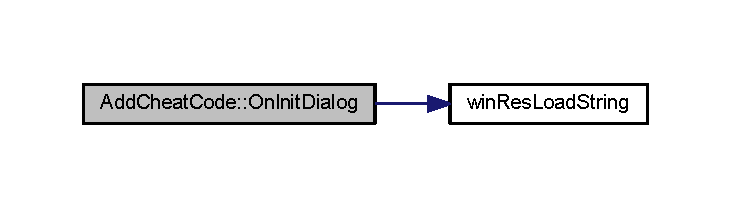
\includegraphics[width=350pt]{class_add_cheat_code_a7818441d921e63c1b0983e86b60beeba_cgraph}
\end{center}
\end{figure}
\mbox{\Hypertarget{class_add_cheat_code_a77b1ec1f5e067495aef92a2f9b8750c8}\label{class_add_cheat_code_a77b1ec1f5e067495aef92a2f9b8750c8}} 
\index{Add\+Cheat\+Code@{Add\+Cheat\+Code}!On\+Ok@{On\+Ok}}
\index{On\+Ok@{On\+Ok}!Add\+Cheat\+Code@{Add\+Cheat\+Code}}
\subsubsection{\texorpdfstring{On\+Ok()}{OnOk()}}
{\footnotesize\ttfamily void Add\+Cheat\+Code\+::\+On\+Ok (\begin{DoxyParamCaption}{ }\end{DoxyParamCaption})\hspace{0.3cm}{\ttfamily [protected]}}



G\+B\+A\+Cheats.\+cpp 파일의 1135 번째 라인에서 정의되었습니다.


\begin{DoxyCode}
1136 \{
1137   CString desc;
1138   CString \mbox{\hyperlink{_g_b_a_8cpp_a28d4d3d8445e73a696b2d6f7eadabd96}{buffer}};
1139   CString token;
1140 
1141   \mbox{\hyperlink{class_add_cheat_code_a9ae1d05acf10bc6fc8ea8cce2ec2cc6a}{m\_code}}.GetWindowText(\mbox{\hyperlink{_g_b_a_8cpp_a28d4d3d8445e73a696b2d6f7eadabd96}{buffer}});
1142   \mbox{\hyperlink{class_add_cheat_code_a5bbe6b54e71db26da7b3abc7449b3342}{m\_desc}}.GetWindowText(desc);
1143   
1144   \mbox{\hyperlink{class_string_tokenizer}{StringTokenizer}} st(\mbox{\hyperlink{_g_b_a_8cpp_a28d4d3d8445e73a696b2d6f7eadabd96}{buffer}}, \textcolor{stringliteral}{" \(\backslash\)t\(\backslash\)n\(\backslash\)r"});
1145   \textcolor{keyword}{const} \textcolor{keywordtype}{char} *\mbox{\hyperlink{expr_8cpp_aded116371789db1fd63c90ef00c95a3d}{t}} = st.next();
1146   \textcolor{keywordflow}{while}(\mbox{\hyperlink{expr_8cpp_aded116371789db1fd63c90ef00c95a3d}{t}}) \{
1147     token = \mbox{\hyperlink{expr_8cpp_aded116371789db1fd63c90ef00c95a3d}{t}};
1148     token.MakeUpper();
1149     \mbox{\hyperlink{_cheats_8cpp_a0e87699a326f10639902f59174a7e6ee}{cheatsAddCheatCode}}(token, desc);
1150     \mbox{\hyperlink{expr_8cpp_aded116371789db1fd63c90ef00c95a3d}{t}} = st.next();
1151   \}
1152   EndDialog(TRUE);
1153 \}
\end{DoxyCode}
이 함수 내부에서 호출하는 함수들에 대한 그래프입니다.\+:
\nopagebreak
\begin{figure}[H]
\begin{center}
\leavevmode
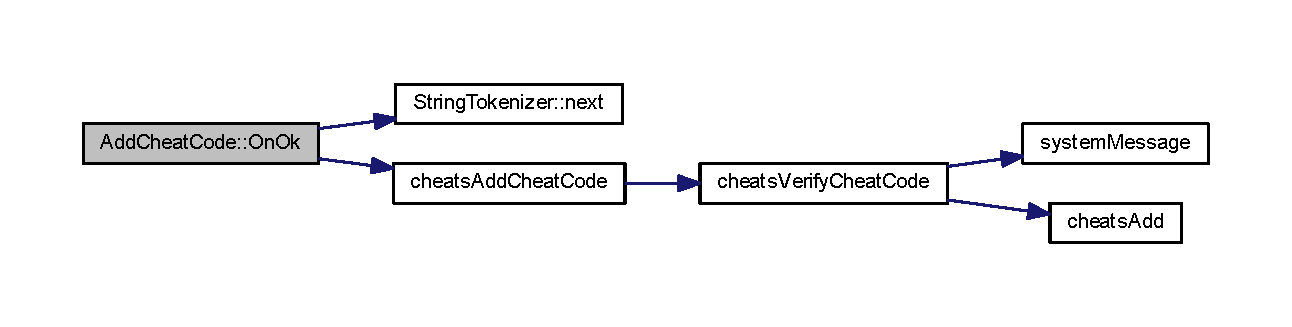
\includegraphics[width=350pt]{class_add_cheat_code_a77b1ec1f5e067495aef92a2f9b8750c8_cgraph}
\end{center}
\end{figure}


\subsection{멤버 데이터 문서화}
\mbox{\Hypertarget{class_add_cheat_code_a9ae1d05acf10bc6fc8ea8cce2ec2cc6a}\label{class_add_cheat_code_a9ae1d05acf10bc6fc8ea8cce2ec2cc6a}} 
\index{Add\+Cheat\+Code@{Add\+Cheat\+Code}!m\+\_\+code@{m\+\_\+code}}
\index{m\+\_\+code@{m\+\_\+code}!Add\+Cheat\+Code@{Add\+Cheat\+Code}}
\subsubsection{\texorpdfstring{m\+\_\+code}{m\_code}}
{\footnotesize\ttfamily C\+Edit Add\+Cheat\+Code\+::m\+\_\+code}



G\+B\+A\+Cheats.\+h 파일의 266 번째 라인에서 정의되었습니다.

\mbox{\Hypertarget{class_add_cheat_code_a5bbe6b54e71db26da7b3abc7449b3342}\label{class_add_cheat_code_a5bbe6b54e71db26da7b3abc7449b3342}} 
\index{Add\+Cheat\+Code@{Add\+Cheat\+Code}!m\+\_\+desc@{m\+\_\+desc}}
\index{m\+\_\+desc@{m\+\_\+desc}!Add\+Cheat\+Code@{Add\+Cheat\+Code}}
\subsubsection{\texorpdfstring{m\+\_\+desc}{m\_desc}}
{\footnotesize\ttfamily C\+Edit Add\+Cheat\+Code\+::m\+\_\+desc}



G\+B\+A\+Cheats.\+h 파일의 265 번째 라인에서 정의되었습니다.



이 클래스에 대한 문서화 페이지는 다음의 파일들로부터 생성되었습니다.\+:\begin{DoxyCompactItemize}
\item 
C\+:/\+Users/sjh13/sources/\+Visual\+Boy\+Advance/src/win32/\mbox{\hyperlink{_g_b_a_cheats_8h}{G\+B\+A\+Cheats.\+h}}\item 
C\+:/\+Users/sjh13/sources/\+Visual\+Boy\+Advance/src/win32/\mbox{\hyperlink{_g_b_a_cheats_8cpp}{G\+B\+A\+Cheats.\+cpp}}\end{DoxyCompactItemize}

\hypertarget{class_add_g_b_cheat}{}\section{Add\+G\+B\+Cheat 클래스 참조}
\label{class_add_g_b_cheat}\index{Add\+G\+B\+Cheat@{Add\+G\+B\+Cheat}}
Add\+G\+B\+Cheat에 대한 상속 다이어그램 \+: \begin{figure}[H]
\begin{center}
\leavevmode
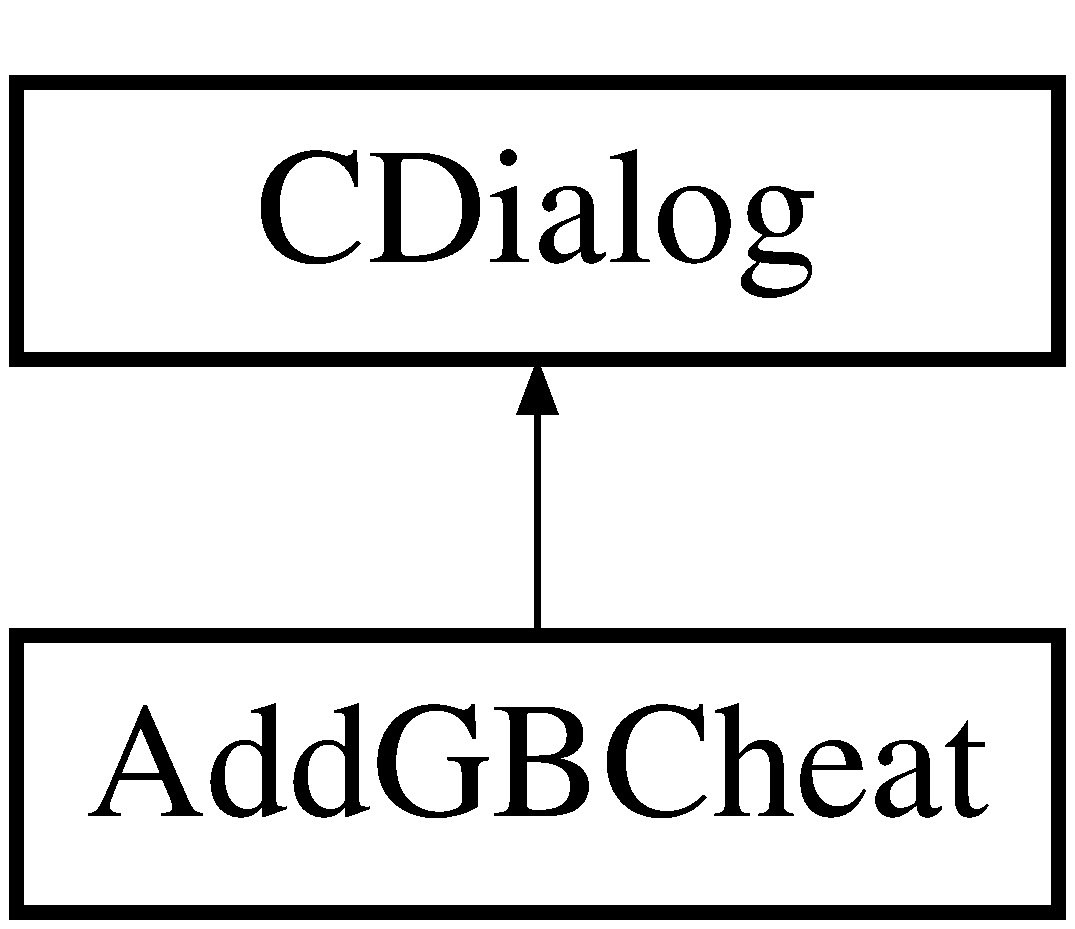
\includegraphics[height=2.000000cm]{class_add_g_b_cheat}
\end{center}
\end{figure}
\subsection*{Public 타입}
\begin{DoxyCompactItemize}
\item 
\mbox{\Hypertarget{class_add_g_b_cheat_ae307c54936e2ef002f6323ab0d1fa05e}\label{class_add_g_b_cheat_ae307c54936e2ef002f6323ab0d1fa05e}} 
enum \{ {\bfseries I\+DD} = I\+D\+D\+\_\+\+A\+D\+D\+\_\+\+C\+H\+E\+AT
 \}
\end{DoxyCompactItemize}
\subsection*{Public 멤버 함수}
\begin{DoxyCompactItemize}
\item 
\mbox{\Hypertarget{class_add_g_b_cheat_a9bff22f01c72ffbcd6071bb604c2e090}\label{class_add_g_b_cheat_a9bff22f01c72ffbcd6071bb604c2e090}} 
afx\+\_\+msg void {\bfseries On\+Size\+Type} (U\+I\+NT id)
\item 
\mbox{\Hypertarget{class_add_g_b_cheat_a1bfddb9d66e182dedc95bf889dc9e6d2}\label{class_add_g_b_cheat_a1bfddb9d66e182dedc95bf889dc9e6d2}} 
afx\+\_\+msg void {\bfseries On\+Number\+Type} (U\+I\+NT id)
\item 
\mbox{\Hypertarget{class_add_g_b_cheat_a054ba5040a40f7ef4b3a0ddb5a458592}\label{class_add_g_b_cheat_a054ba5040a40f7ef4b3a0ddb5a458592}} 
bool {\bfseries add\+Cheat} ()
\item 
\mbox{\Hypertarget{class_add_g_b_cheat_a1794ccc1e4826b5a8b179d20557955b8}\label{class_add_g_b_cheat_a1794ccc1e4826b5a8b179d20557955b8}} 
{\bfseries Add\+G\+B\+Cheat} (u32 addr, C\+Wnd $\ast$p\+Parent=N\+U\+LL)
\end{DoxyCompactItemize}
\subsection*{Public 속성}
\begin{DoxyCompactItemize}
\item 
\mbox{\Hypertarget{class_add_g_b_cheat_ac5705ad3d8964adb59d62c51dd60a0fc}\label{class_add_g_b_cheat_ac5705ad3d8964adb59d62c51dd60a0fc}} 
C\+Edit {\bfseries m\+\_\+value}
\item 
\mbox{\Hypertarget{class_add_g_b_cheat_af68f821a3073c6a01f1c8760dab628ee}\label{class_add_g_b_cheat_af68f821a3073c6a01f1c8760dab628ee}} 
C\+Edit {\bfseries m\+\_\+address}
\item 
\mbox{\Hypertarget{class_add_g_b_cheat_ae1711f59505d7d442a6572a346993cd2}\label{class_add_g_b_cheat_ae1711f59505d7d442a6572a346993cd2}} 
C\+Edit {\bfseries m\+\_\+desc}
\item 
\mbox{\Hypertarget{class_add_g_b_cheat_ae0603ce2570d5b09a64f4bd6c2107962}\label{class_add_g_b_cheat_ae0603ce2570d5b09a64f4bd6c2107962}} 
int {\bfseries size\+Type}
\item 
\mbox{\Hypertarget{class_add_g_b_cheat_ab49fa34156026418e26edf606aa82b1a}\label{class_add_g_b_cheat_ab49fa34156026418e26edf606aa82b1a}} 
int {\bfseries number\+Type}
\end{DoxyCompactItemize}
\subsection*{Protected 멤버 함수}
\begin{DoxyCompactItemize}
\item 
\mbox{\Hypertarget{class_add_g_b_cheat_ab90d0a5d50911d10eec2706250882d6f}\label{class_add_g_b_cheat_ab90d0a5d50911d10eec2706250882d6f}} 
virtual void {\bfseries Do\+Data\+Exchange} (C\+Data\+Exchange $\ast$p\+DX)
\item 
\mbox{\Hypertarget{class_add_g_b_cheat_ac2eb6674e040b6a8af227e6517f857e8}\label{class_add_g_b_cheat_ac2eb6674e040b6a8af227e6517f857e8}} 
afx\+\_\+msg void {\bfseries On\+Cancel} ()
\item 
\mbox{\Hypertarget{class_add_g_b_cheat_aef6d73f3cdf51e28bbba9f7e14b21941}\label{class_add_g_b_cheat_aef6d73f3cdf51e28bbba9f7e14b21941}} 
afx\+\_\+msg void {\bfseries On\+Ok} ()
\item 
\mbox{\Hypertarget{class_add_g_b_cheat_a97210ad566b117af4994adac5d954e94}\label{class_add_g_b_cheat_a97210ad566b117af4994adac5d954e94}} 
virtual B\+O\+OL {\bfseries On\+Init\+Dialog} ()
\end{DoxyCompactItemize}
\subsection*{Protected 속성}
\begin{DoxyCompactItemize}
\item 
\mbox{\Hypertarget{class_add_g_b_cheat_adb910488c84e165b4fd33646b932ee2e}\label{class_add_g_b_cheat_adb910488c84e165b4fd33646b932ee2e}} 
L\+O\+N\+G\+\_\+\+P\+TR {\bfseries address}
\end{DoxyCompactItemize}


이 클래스에 대한 문서화 페이지는 다음의 파일들로부터 생성되었습니다.\+:\begin{DoxyCompactItemize}
\item 
src/win32/G\+B\+Cheats\+Dlg.\+h\item 
src/win32/G\+B\+Cheats\+Dlg.\+cpp\end{DoxyCompactItemize}

\hypertarget{class_add_g_b_code}{}\section{Add\+G\+B\+Code 클래스 참조}
\label{class_add_g_b_code}\index{Add\+G\+B\+Code@{Add\+G\+B\+Code}}
Add\+G\+B\+Code에 대한 상속 다이어그램 \+: \begin{figure}[H]
\begin{center}
\leavevmode
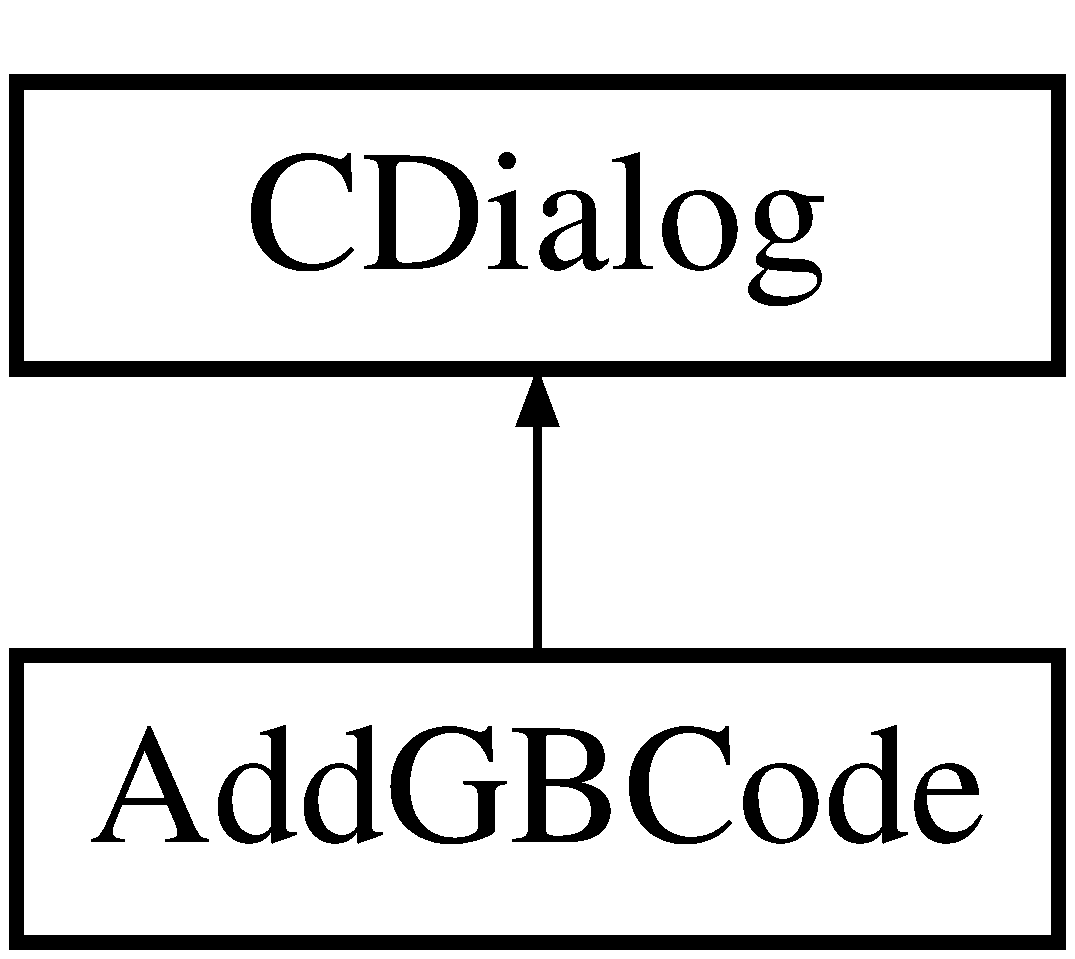
\includegraphics[height=2.000000cm]{class_add_g_b_code}
\end{center}
\end{figure}
\subsection*{Public 타입}
\begin{DoxyCompactItemize}
\item 
\mbox{\Hypertarget{class_add_g_b_code_a2dd2d84fa89620e9d1bd9816ac698df9}\label{class_add_g_b_code_a2dd2d84fa89620e9d1bd9816ac698df9}} 
enum \{ {\bfseries I\+DD} = I\+D\+D\+\_\+\+A\+D\+D\+\_\+\+C\+H\+E\+A\+T\+\_\+\+D\+LG
 \}
\end{DoxyCompactItemize}
\subsection*{Public 멤버 함수}
\begin{DoxyCompactItemize}
\item 
\mbox{\Hypertarget{class_add_g_b_code_a99be74c9c22f954a6a83fb1e8eba7b29}\label{class_add_g_b_code_a99be74c9c22f954a6a83fb1e8eba7b29}} 
{\bfseries Add\+G\+B\+Code} (bool($\ast$verify)(const char $\ast$, const char $\ast$), int, const char $\ast$, C\+Wnd $\ast$p\+Parent=N\+U\+LL)
\end{DoxyCompactItemize}
\subsection*{Public 속성}
\begin{DoxyCompactItemize}
\item 
\mbox{\Hypertarget{class_add_g_b_code_af67488ee0354c39ce9c818e7f389e74f}\label{class_add_g_b_code_af67488ee0354c39ce9c818e7f389e74f}} 
C\+Edit {\bfseries m\+\_\+desc}
\item 
\mbox{\Hypertarget{class_add_g_b_code_a1336063b1498bee29c2a9df7273d8ca9}\label{class_add_g_b_code_a1336063b1498bee29c2a9df7273d8ca9}} 
C\+Edit {\bfseries m\+\_\+code}
\item 
\mbox{\Hypertarget{class_add_g_b_code_abed904b4077498637455cbd6f829a742}\label{class_add_g_b_code_abed904b4077498637455cbd6f829a742}} 
int {\bfseries add\+Length}
\item 
\mbox{\Hypertarget{class_add_g_b_code_a436954b9aea5bac8b7063a6939f829ae}\label{class_add_g_b_code_a436954b9aea5bac8b7063a6939f829ae}} 
C\+String {\bfseries add\+Title}
\item 
\mbox{\Hypertarget{class_add_g_b_code_a3c81ddb0e728491632442e95218f40cf}\label{class_add_g_b_code_a3c81ddb0e728491632442e95218f40cf}} 
bool($\ast$ {\bfseries add\+Verify} )(const char $\ast$, const char $\ast$)
\end{DoxyCompactItemize}
\subsection*{Protected 멤버 함수}
\begin{DoxyCompactItemize}
\item 
\mbox{\Hypertarget{class_add_g_b_code_a7ae9f69b6acec1cb7816dc4959ba0b1c}\label{class_add_g_b_code_a7ae9f69b6acec1cb7816dc4959ba0b1c}} 
virtual void {\bfseries Do\+Data\+Exchange} (C\+Data\+Exchange $\ast$p\+DX)
\item 
\mbox{\Hypertarget{class_add_g_b_code_ad6bdbbb8375531b30329c5ab4689c052}\label{class_add_g_b_code_ad6bdbbb8375531b30329c5ab4689c052}} 
afx\+\_\+msg void {\bfseries On\+Ok} ()
\item 
\mbox{\Hypertarget{class_add_g_b_code_a0ebf90bce5407457b60eb77237adec17}\label{class_add_g_b_code_a0ebf90bce5407457b60eb77237adec17}} 
afx\+\_\+msg void {\bfseries On\+Cancel} ()
\item 
\mbox{\Hypertarget{class_add_g_b_code_a1f7ec5a04ded3dee0016552b0961ffba}\label{class_add_g_b_code_a1f7ec5a04ded3dee0016552b0961ffba}} 
virtual B\+O\+OL {\bfseries On\+Init\+Dialog} ()
\end{DoxyCompactItemize}


이 클래스에 대한 문서화 페이지는 다음의 파일들로부터 생성되었습니다.\+:\begin{DoxyCompactItemize}
\item 
src/win32/G\+B\+Cheats\+Dlg.\+h\item 
src/win32/G\+B\+Cheats\+Dlg.\+cpp\end{DoxyCompactItemize}

\hypertarget{class_add_g_s_a_code}{}\section{Add\+G\+S\+A\+Code 클래스 참조}
\label{class_add_g_s_a_code}\index{Add\+G\+S\+A\+Code@{Add\+G\+S\+A\+Code}}


{\ttfamily \#include $<$G\+B\+A\+Cheats.\+h$>$}



Add\+G\+S\+A\+Code에 대한 상속 다이어그램 \+: \nopagebreak
\begin{figure}[H]
\begin{center}
\leavevmode
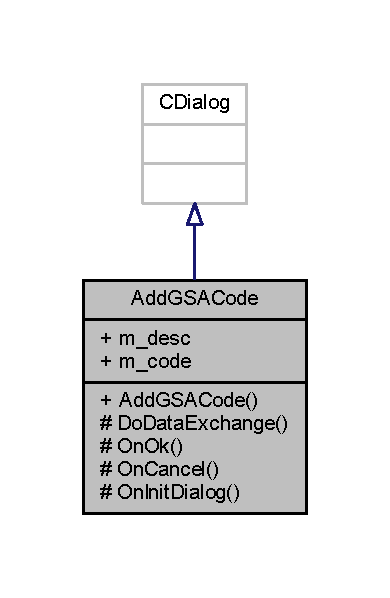
\includegraphics[width=187pt]{class_add_g_s_a_code__inherit__graph}
\end{center}
\end{figure}


Add\+G\+S\+A\+Code에 대한 협력 다이어그램\+:\nopagebreak
\begin{figure}[H]
\begin{center}
\leavevmode
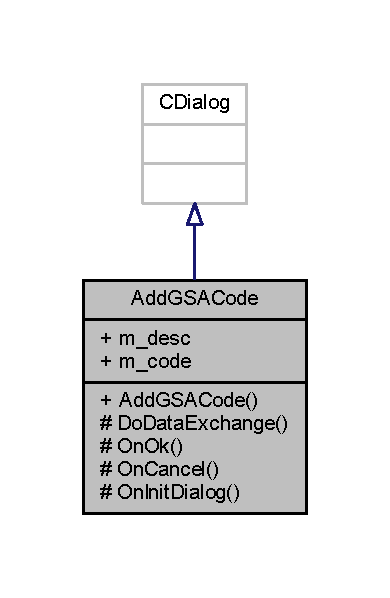
\includegraphics[width=187pt]{class_add_g_s_a_code__coll__graph}
\end{center}
\end{figure}
\subsection*{Public 타입}
\begin{DoxyCompactItemize}
\item 
enum \{ \mbox{\hyperlink{class_add_g_s_a_code_ae09fbbcc1c447c677bf62ee2bcf7c945ade7716d104ed702a0c8cb0e4b61f64f4}{I\+DD}} = I\+D\+D\+\_\+\+A\+D\+D\+\_\+\+C\+H\+E\+A\+T\+\_\+\+D\+LG
 \}
\end{DoxyCompactItemize}
\subsection*{Public 멤버 함수}
\begin{DoxyCompactItemize}
\item 
\mbox{\hyperlink{class_add_g_s_a_code_adae37d67fa94fcd376ae11c6d9bd9d01}{Add\+G\+S\+A\+Code}} (C\+Wnd $\ast$p\+Parent=\mbox{\hyperlink{_system_8h_a070d2ce7b6bb7e5c05602aa8c308d0c4}{N\+U\+LL}})
\end{DoxyCompactItemize}
\subsection*{Public 속성}
\begin{DoxyCompactItemize}
\item 
C\+Edit \mbox{\hyperlink{class_add_g_s_a_code_a766cb9061a235616a856d3c1b16879db}{m\+\_\+desc}}
\item 
C\+Edit \mbox{\hyperlink{class_add_g_s_a_code_a0a4c3486121bd6be93e8f64215fea1ab}{m\+\_\+code}}
\end{DoxyCompactItemize}
\subsection*{Protected 멤버 함수}
\begin{DoxyCompactItemize}
\item 
virtual void \mbox{\hyperlink{class_add_g_s_a_code_a28d3f80ce066475e3d67e7fe62bb1f73}{Do\+Data\+Exchange}} (C\+Data\+Exchange $\ast$p\+DX)
\item 
afx\+\_\+msg void \mbox{\hyperlink{class_add_g_s_a_code_a857608ad314694d15ee6e811fb528d0b}{On\+Ok}} ()
\item 
afx\+\_\+msg void \mbox{\hyperlink{class_add_g_s_a_code_aa0db7ac66785e11cd5f614a06f7a11a2}{On\+Cancel}} ()
\item 
virtual B\+O\+OL \mbox{\hyperlink{class_add_g_s_a_code_af6ea2661ff2da964833f9e86f88cb1ff}{On\+Init\+Dialog}} ()
\end{DoxyCompactItemize}


\subsection{상세한 설명}


G\+B\+A\+Cheats.\+h 파일의 184 번째 라인에서 정의되었습니다.



\subsection{멤버 열거형 문서화}
\mbox{\Hypertarget{class_add_g_s_a_code_ae09fbbcc1c447c677bf62ee2bcf7c945}\label{class_add_g_s_a_code_ae09fbbcc1c447c677bf62ee2bcf7c945}} 
\subsubsection{\texorpdfstring{anonymous enum}{anonymous enum}}
{\footnotesize\ttfamily anonymous enum}

\begin{DoxyEnumFields}{열거형 멤버}
\raisebox{\heightof{T}}[0pt][0pt]{\index{I\+DD@{I\+DD}!Add\+G\+S\+A\+Code@{Add\+G\+S\+A\+Code}}\index{Add\+G\+S\+A\+Code@{Add\+G\+S\+A\+Code}!I\+DD@{I\+DD}}}\mbox{\Hypertarget{class_add_g_s_a_code_ae09fbbcc1c447c677bf62ee2bcf7c945ade7716d104ed702a0c8cb0e4b61f64f4}\label{class_add_g_s_a_code_ae09fbbcc1c447c677bf62ee2bcf7c945ade7716d104ed702a0c8cb0e4b61f64f4}} 
I\+DD&\\
\hline

\end{DoxyEnumFields}


G\+B\+A\+Cheats.\+h 파일의 192 번째 라인에서 정의되었습니다.


\begin{DoxyCode}
192 \{ \mbox{\hyperlink{class_add_g_s_a_code_ae09fbbcc1c447c677bf62ee2bcf7c945ade7716d104ed702a0c8cb0e4b61f64f4}{IDD}} = \mbox{\hyperlink{resource_8h_a388a8d7b6dea32798ece69044a21790d}{IDD\_ADD\_CHEAT\_DLG}} \};
\end{DoxyCode}


\subsection{생성자 \& 소멸자 문서화}
\mbox{\Hypertarget{class_add_g_s_a_code_adae37d67fa94fcd376ae11c6d9bd9d01}\label{class_add_g_s_a_code_adae37d67fa94fcd376ae11c6d9bd9d01}} 
\index{Add\+G\+S\+A\+Code@{Add\+G\+S\+A\+Code}!Add\+G\+S\+A\+Code@{Add\+G\+S\+A\+Code}}
\index{Add\+G\+S\+A\+Code@{Add\+G\+S\+A\+Code}!Add\+G\+S\+A\+Code@{Add\+G\+S\+A\+Code}}
\subsubsection{\texorpdfstring{Add\+G\+S\+A\+Code()}{AddGSACode()}}
{\footnotesize\ttfamily Add\+G\+S\+A\+Code\+::\+Add\+G\+S\+A\+Code (\begin{DoxyParamCaption}\item[{C\+Wnd $\ast$}]{p\+Parent = {\ttfamily \mbox{\hyperlink{_system_8h_a070d2ce7b6bb7e5c05602aa8c308d0c4}{N\+U\+LL}}} }\end{DoxyParamCaption})}



G\+B\+A\+Cheats.\+cpp 파일의 914 번째 라인에서 정의되었습니다.


\begin{DoxyCode}
915   : CDialog(\mbox{\hyperlink{class_add_g_s_a_code_ae09fbbcc1c447c677bf62ee2bcf7c945ade7716d104ed702a0c8cb0e4b61f64f4}{AddGSACode::IDD}}, pParent)
916 \{
917   \textcolor{comment}{//\{\{AFX\_DATA\_INIT(AddGSACode)}
918   \textcolor{comment}{// NOTE: the ClassWizard will add member initialization here}
919   \textcolor{comment}{//\}\}AFX\_DATA\_INIT}
920 \}
\end{DoxyCode}


\subsection{멤버 함수 문서화}
\mbox{\Hypertarget{class_add_g_s_a_code_a28d3f80ce066475e3d67e7fe62bb1f73}\label{class_add_g_s_a_code_a28d3f80ce066475e3d67e7fe62bb1f73}} 
\index{Add\+G\+S\+A\+Code@{Add\+G\+S\+A\+Code}!Do\+Data\+Exchange@{Do\+Data\+Exchange}}
\index{Do\+Data\+Exchange@{Do\+Data\+Exchange}!Add\+G\+S\+A\+Code@{Add\+G\+S\+A\+Code}}
\subsubsection{\texorpdfstring{Do\+Data\+Exchange()}{DoDataExchange()}}
{\footnotesize\ttfamily void Add\+G\+S\+A\+Code\+::\+Do\+Data\+Exchange (\begin{DoxyParamCaption}\item[{C\+Data\+Exchange $\ast$}]{p\+DX }\end{DoxyParamCaption})\hspace{0.3cm}{\ttfamily [protected]}, {\ttfamily [virtual]}}



G\+B\+A\+Cheats.\+cpp 파일의 923 번째 라인에서 정의되었습니다.


\begin{DoxyCode}
924 \{
925   CDialog::DoDataExchange(pDX);
926   \textcolor{comment}{//\{\{AFX\_DATA\_MAP(AddGSACode)}
927   DDX\_Control(pDX, \mbox{\hyperlink{resource_8h_adb05cf1e74135587a9b3ab93a5152feb}{IDC\_DESC}}, \mbox{\hyperlink{class_add_g_s_a_code_a766cb9061a235616a856d3c1b16879db}{m\_desc}});
928   DDX\_Control(pDX, \mbox{\hyperlink{resource_8h_abb149f0043fd3834639ddb2d80d31723}{IDC\_CODE}}, \mbox{\hyperlink{class_add_g_s_a_code_a0a4c3486121bd6be93e8f64215fea1ab}{m\_code}});
929   \textcolor{comment}{//\}\}AFX\_DATA\_MAP}
930 \}
\end{DoxyCode}
\mbox{\Hypertarget{class_add_g_s_a_code_aa0db7ac66785e11cd5f614a06f7a11a2}\label{class_add_g_s_a_code_aa0db7ac66785e11cd5f614a06f7a11a2}} 
\index{Add\+G\+S\+A\+Code@{Add\+G\+S\+A\+Code}!On\+Cancel@{On\+Cancel}}
\index{On\+Cancel@{On\+Cancel}!Add\+G\+S\+A\+Code@{Add\+G\+S\+A\+Code}}
\subsubsection{\texorpdfstring{On\+Cancel()}{OnCancel()}}
{\footnotesize\ttfamily void Add\+G\+S\+A\+Code\+::\+On\+Cancel (\begin{DoxyParamCaption}{ }\end{DoxyParamCaption})\hspace{0.3cm}{\ttfamily [protected]}}



G\+B\+A\+Cheats.\+cpp 파일의 987 번째 라인에서 정의되었습니다.


\begin{DoxyCode}
988 \{
989   EndDialog(FALSE);
990 \}
\end{DoxyCode}
\mbox{\Hypertarget{class_add_g_s_a_code_af6ea2661ff2da964833f9e86f88cb1ff}\label{class_add_g_s_a_code_af6ea2661ff2da964833f9e86f88cb1ff}} 
\index{Add\+G\+S\+A\+Code@{Add\+G\+S\+A\+Code}!On\+Init\+Dialog@{On\+Init\+Dialog}}
\index{On\+Init\+Dialog@{On\+Init\+Dialog}!Add\+G\+S\+A\+Code@{Add\+G\+S\+A\+Code}}
\subsubsection{\texorpdfstring{On\+Init\+Dialog()}{OnInitDialog()}}
{\footnotesize\ttfamily B\+O\+OL Add\+G\+S\+A\+Code\+::\+On\+Init\+Dialog (\begin{DoxyParamCaption}{ }\end{DoxyParamCaption})\hspace{0.3cm}{\ttfamily [protected]}, {\ttfamily [virtual]}}



G\+B\+A\+Cheats.\+cpp 파일의 992 번째 라인에서 정의되었습니다.


\begin{DoxyCode}
993 \{
994   CDialog::OnInitDialog();
995   
996   \mbox{\hyperlink{class_add_g_s_a_code_a0a4c3486121bd6be93e8f64215fea1ab}{m\_code}}.LimitText(1024);
997   \mbox{\hyperlink{class_add_g_s_a_code_a766cb9061a235616a856d3c1b16879db}{m\_desc}}.LimitText(32);
998   CString title = \mbox{\hyperlink{_win_res_util_8cpp_a416e85e80ab9b01376e87251c83d1a5a}{winResLoadString}}(\mbox{\hyperlink{resource_8h_a49836eba8e0beeff1d7e166eea41a5eb}{IDS\_ADD\_GSA\_CODE}});
999   SetWindowText(title);
1000   CenterWindow();
1001   
1002   \textcolor{keywordflow}{return} TRUE;  \textcolor{comment}{// return TRUE unless you set the focus to a control}
1003                 \textcolor{comment}{// EXCEPTION: OCX Property Pages should return FALSE}
1004 \}
\end{DoxyCode}
이 함수 내부에서 호출하는 함수들에 대한 그래프입니다.\+:
\nopagebreak
\begin{figure}[H]
\begin{center}
\leavevmode
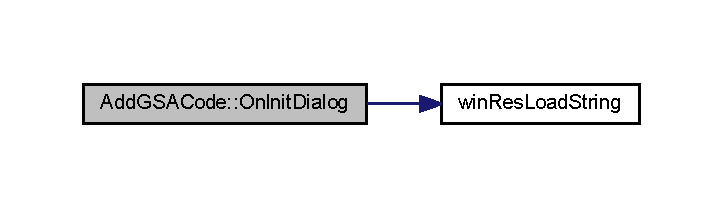
\includegraphics[width=347pt]{class_add_g_s_a_code_af6ea2661ff2da964833f9e86f88cb1ff_cgraph}
\end{center}
\end{figure}
\mbox{\Hypertarget{class_add_g_s_a_code_a857608ad314694d15ee6e811fb528d0b}\label{class_add_g_s_a_code_a857608ad314694d15ee6e811fb528d0b}} 
\index{Add\+G\+S\+A\+Code@{Add\+G\+S\+A\+Code}!On\+Ok@{On\+Ok}}
\index{On\+Ok@{On\+Ok}!Add\+G\+S\+A\+Code@{Add\+G\+S\+A\+Code}}
\subsubsection{\texorpdfstring{On\+Ok()}{OnOk()}}
{\footnotesize\ttfamily void Add\+G\+S\+A\+Code\+::\+On\+Ok (\begin{DoxyParamCaption}{ }\end{DoxyParamCaption})\hspace{0.3cm}{\ttfamily [protected]}}



G\+B\+A\+Cheats.\+cpp 파일의 943 번째 라인에서 정의되었습니다.


\begin{DoxyCode}
944 \{
945   CString desc;
946   CString \mbox{\hyperlink{_g_b_a_8cpp_a28d4d3d8445e73a696b2d6f7eadabd96}{buffer}};
947   CString part1;
948   CString code;
949   CString token;  
950 
951   \mbox{\hyperlink{class_add_g_s_a_code_a0a4c3486121bd6be93e8f64215fea1ab}{m\_code}}.GetWindowText(\mbox{\hyperlink{_g_b_a_8cpp_a28d4d3d8445e73a696b2d6f7eadabd96}{buffer}});
952   \mbox{\hyperlink{class_add_g_s_a_code_a766cb9061a235616a856d3c1b16879db}{m\_desc}}.GetWindowText(desc);
953   
954   \mbox{\hyperlink{class_string_tokenizer}{StringTokenizer}} st(\mbox{\hyperlink{_g_b_a_8cpp_a28d4d3d8445e73a696b2d6f7eadabd96}{buffer}}, \textcolor{stringliteral}{" \(\backslash\)t\(\backslash\)n\(\backslash\)r"});
955   part1.Empty();
956   \textcolor{keyword}{const} \textcolor{keywordtype}{char} *\mbox{\hyperlink{expr_8cpp_aded116371789db1fd63c90ef00c95a3d}{t}} = st.next();
957   \textcolor{keywordflow}{while}(\mbox{\hyperlink{expr_8cpp_aded116371789db1fd63c90ef00c95a3d}{t}}) \{
958     token = \mbox{\hyperlink{expr_8cpp_aded116371789db1fd63c90ef00c95a3d}{t}};
959     token.MakeUpper();
960     \textcolor{keywordflow}{if}(token.GetLength() == 16)
961       \mbox{\hyperlink{_cheats_8cpp_a47aded7deffcbfa36ed55944eafb72ab}{cheatsAddGSACode}}(token, desc, \textcolor{keyword}{false});
962     \textcolor{keywordflow}{else} \textcolor{keywordflow}{if}(token.GetLength() == 12) \{
963       code = token.Left(8);
964       code += \textcolor{stringliteral}{" "};
965       code += token.Right(4);
966       \mbox{\hyperlink{_cheats_8cpp_af79d349aaea63793beec4fa2626f74c8}{cheatsAddCBACode}}(code, desc);
967     \} \textcolor{keywordflow}{else} \textcolor{keywordflow}{if}(part1.IsEmpty())
968       part1 = token;
969     \textcolor{keywordflow}{else} \{
970       \textcolor{keywordflow}{if}(token.GetLength() == 4) \{
971         code = part1;
972         code += \textcolor{stringliteral}{" "};
973         code += token;
974         \mbox{\hyperlink{_cheats_8cpp_af79d349aaea63793beec4fa2626f74c8}{cheatsAddCBACode}}(code, desc);
975       \} \textcolor{keywordflow}{else} \{
976         code = part1 + token;
977         \mbox{\hyperlink{_cheats_8cpp_a47aded7deffcbfa36ed55944eafb72ab}{cheatsAddGSACode}}(code, desc, \textcolor{keyword}{true});
978       \}
979       part1.Empty();
980     \}
981 
982     \mbox{\hyperlink{expr_8cpp_aded116371789db1fd63c90ef00c95a3d}{t}} = st.next();
983   \}
984   EndDialog(TRUE);
985 \}
\end{DoxyCode}
이 함수 내부에서 호출하는 함수들에 대한 그래프입니다.\+:
\nopagebreak
\begin{figure}[H]
\begin{center}
\leavevmode
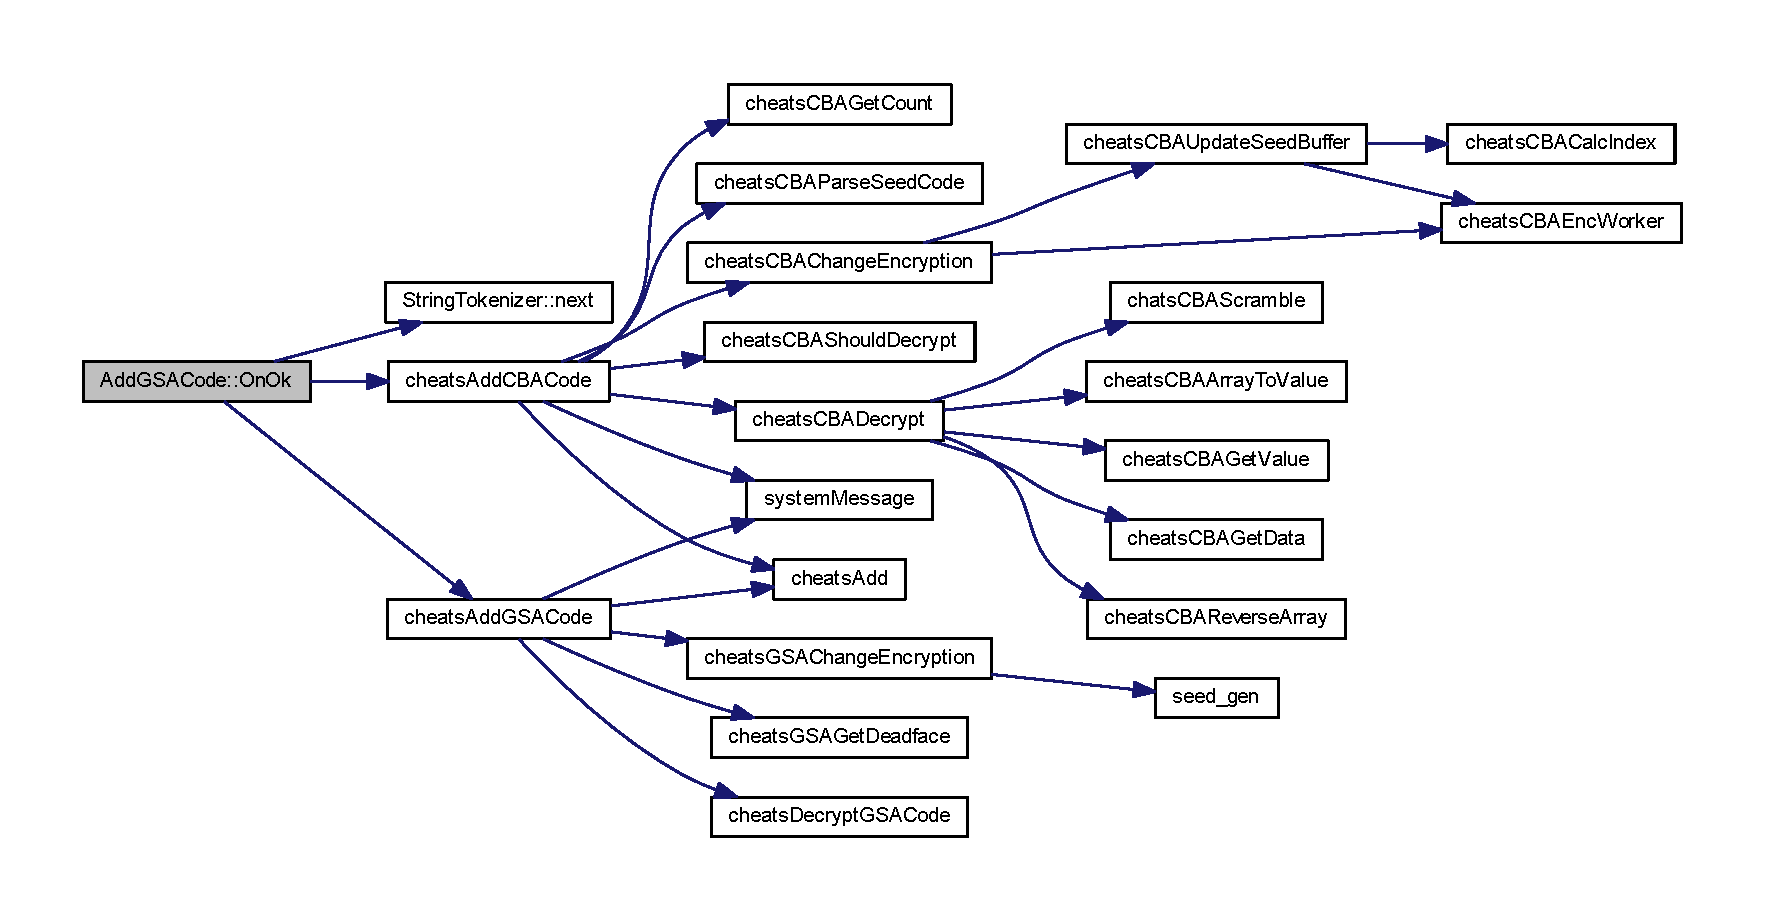
\includegraphics[width=350pt]{class_add_g_s_a_code_a857608ad314694d15ee6e811fb528d0b_cgraph}
\end{center}
\end{figure}


\subsection{멤버 데이터 문서화}
\mbox{\Hypertarget{class_add_g_s_a_code_a0a4c3486121bd6be93e8f64215fea1ab}\label{class_add_g_s_a_code_a0a4c3486121bd6be93e8f64215fea1ab}} 
\index{Add\+G\+S\+A\+Code@{Add\+G\+S\+A\+Code}!m\+\_\+code@{m\+\_\+code}}
\index{m\+\_\+code@{m\+\_\+code}!Add\+G\+S\+A\+Code@{Add\+G\+S\+A\+Code}}
\subsubsection{\texorpdfstring{m\+\_\+code}{m\_code}}
{\footnotesize\ttfamily C\+Edit Add\+G\+S\+A\+Code\+::m\+\_\+code}



G\+B\+A\+Cheats.\+h 파일의 194 번째 라인에서 정의되었습니다.

\mbox{\Hypertarget{class_add_g_s_a_code_a766cb9061a235616a856d3c1b16879db}\label{class_add_g_s_a_code_a766cb9061a235616a856d3c1b16879db}} 
\index{Add\+G\+S\+A\+Code@{Add\+G\+S\+A\+Code}!m\+\_\+desc@{m\+\_\+desc}}
\index{m\+\_\+desc@{m\+\_\+desc}!Add\+G\+S\+A\+Code@{Add\+G\+S\+A\+Code}}
\subsubsection{\texorpdfstring{m\+\_\+desc}{m\_desc}}
{\footnotesize\ttfamily C\+Edit Add\+G\+S\+A\+Code\+::m\+\_\+desc}



G\+B\+A\+Cheats.\+h 파일의 193 번째 라인에서 정의되었습니다.



이 클래스에 대한 문서화 페이지는 다음의 파일들로부터 생성되었습니다.\+:\begin{DoxyCompactItemize}
\item 
C\+:/\+Users/sjh13/sources/\+Visual\+Boy\+Advance/src/win32/\mbox{\hyperlink{_g_b_a_cheats_8h}{G\+B\+A\+Cheats.\+h}}\item 
C\+:/\+Users/sjh13/sources/\+Visual\+Boy\+Advance/src/win32/\mbox{\hyperlink{_g_b_a_cheats_8cpp}{G\+B\+A\+Cheats.\+cpp}}\end{DoxyCompactItemize}

\hypertarget{struct_a_range}{}\section{A\+Range 구조체 참조}
\label{struct_a_range}\index{A\+Range@{A\+Range}}


{\ttfamily \#include $<$elf.\+h$>$}



A\+Range에 대한 협력 다이어그램\+:\nopagebreak
\begin{figure}[H]
\begin{center}
\leavevmode
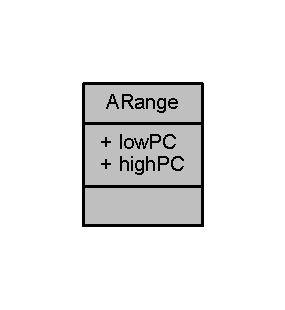
\includegraphics[width=137pt]{struct_a_range__coll__graph}
\end{center}
\end{figure}
\subsection*{Public 속성}
\begin{DoxyCompactItemize}
\item 
\mbox{\hyperlink{_system_8h_a10e94b422ef0c20dcdec20d31a1f5049}{u32}} \mbox{\hyperlink{struct_a_range_a967436344fa630513a70d3fadb4c3bbe}{low\+PC}}
\item 
\mbox{\hyperlink{_system_8h_a10e94b422ef0c20dcdec20d31a1f5049}{u32}} \mbox{\hyperlink{struct_a_range_aa1c1290004480b58c3fb5133e5e00430}{high\+PC}}
\end{DoxyCompactItemize}


\subsection{상세한 설명}


elf.\+h 파일의 220 번째 라인에서 정의되었습니다.



\subsection{멤버 데이터 문서화}
\mbox{\Hypertarget{struct_a_range_aa1c1290004480b58c3fb5133e5e00430}\label{struct_a_range_aa1c1290004480b58c3fb5133e5e00430}} 
\index{A\+Range@{A\+Range}!high\+PC@{high\+PC}}
\index{high\+PC@{high\+PC}!A\+Range@{A\+Range}}
\subsubsection{\texorpdfstring{high\+PC}{highPC}}
{\footnotesize\ttfamily \mbox{\hyperlink{_system_8h_a10e94b422ef0c20dcdec20d31a1f5049}{u32}} A\+Range\+::high\+PC}



elf.\+h 파일의 222 번째 라인에서 정의되었습니다.

\mbox{\Hypertarget{struct_a_range_a967436344fa630513a70d3fadb4c3bbe}\label{struct_a_range_a967436344fa630513a70d3fadb4c3bbe}} 
\index{A\+Range@{A\+Range}!low\+PC@{low\+PC}}
\index{low\+PC@{low\+PC}!A\+Range@{A\+Range}}
\subsubsection{\texorpdfstring{low\+PC}{lowPC}}
{\footnotesize\ttfamily \mbox{\hyperlink{_system_8h_a10e94b422ef0c20dcdec20d31a1f5049}{u32}} A\+Range\+::low\+PC}



elf.\+h 파일의 221 번째 라인에서 정의되었습니다.



이 구조체에 대한 문서화 페이지는 다음의 파일로부터 생성되었습니다.\+:\begin{DoxyCompactItemize}
\item 
C\+:/\+Users/sjh13/sources/\+Visual\+Boy\+Advance/src/\mbox{\hyperlink{elf_8h}{elf.\+h}}\end{DoxyCompactItemize}

\hypertarget{struct_a_ranges}{}\section{A\+Ranges 구조체 참조}
\label{struct_a_ranges}\index{A\+Ranges@{A\+Ranges}}


{\ttfamily \#include $<$elf.\+h$>$}



A\+Ranges에 대한 협력 다이어그램\+:\nopagebreak
\begin{figure}[H]
\begin{center}
\leavevmode
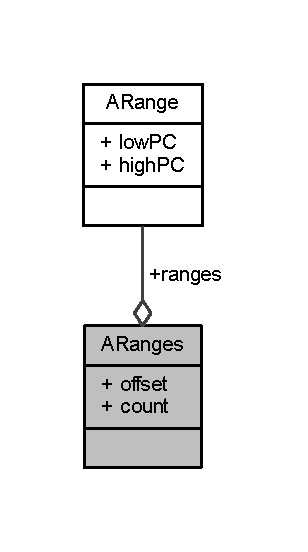
\includegraphics[width=148pt]{struct_a_ranges__coll__graph}
\end{center}
\end{figure}
\subsection*{Public 속성}
\begin{DoxyCompactItemize}
\item 
\mbox{\hyperlink{_system_8h_a10e94b422ef0c20dcdec20d31a1f5049}{u32}} \mbox{\hyperlink{struct_a_ranges_ac9a8655acb6be1e8f52053fc49c34efa}{offset}}
\item 
\mbox{\hyperlink{_util_8cpp_a0ef32aa8672df19503a49fab2d0c8071}{int}} \mbox{\hyperlink{struct_a_ranges_a6f197b7ddb2b3cb334c2eeb9de8d7288}{count}}
\item 
\mbox{\hyperlink{struct_a_range}{A\+Range}} $\ast$ \mbox{\hyperlink{struct_a_ranges_a2eb62f0d43045767640b1d0c4dd8191e}{ranges}}
\end{DoxyCompactItemize}


\subsection{상세한 설명}


elf.\+h 파일의 225 번째 라인에서 정의되었습니다.



\subsection{멤버 데이터 문서화}
\mbox{\Hypertarget{struct_a_ranges_a6f197b7ddb2b3cb334c2eeb9de8d7288}\label{struct_a_ranges_a6f197b7ddb2b3cb334c2eeb9de8d7288}} 
\index{A\+Ranges@{A\+Ranges}!count@{count}}
\index{count@{count}!A\+Ranges@{A\+Ranges}}
\subsubsection{\texorpdfstring{count}{count}}
{\footnotesize\ttfamily \mbox{\hyperlink{_util_8cpp_a0ef32aa8672df19503a49fab2d0c8071}{int}} A\+Ranges\+::count}



elf.\+h 파일의 227 번째 라인에서 정의되었습니다.

\mbox{\Hypertarget{struct_a_ranges_ac9a8655acb6be1e8f52053fc49c34efa}\label{struct_a_ranges_ac9a8655acb6be1e8f52053fc49c34efa}} 
\index{A\+Ranges@{A\+Ranges}!offset@{offset}}
\index{offset@{offset}!A\+Ranges@{A\+Ranges}}
\subsubsection{\texorpdfstring{offset}{offset}}
{\footnotesize\ttfamily \mbox{\hyperlink{_system_8h_a10e94b422ef0c20dcdec20d31a1f5049}{u32}} A\+Ranges\+::offset}



elf.\+h 파일의 226 번째 라인에서 정의되었습니다.

\mbox{\Hypertarget{struct_a_ranges_a2eb62f0d43045767640b1d0c4dd8191e}\label{struct_a_ranges_a2eb62f0d43045767640b1d0c4dd8191e}} 
\index{A\+Ranges@{A\+Ranges}!ranges@{ranges}}
\index{ranges@{ranges}!A\+Ranges@{A\+Ranges}}
\subsubsection{\texorpdfstring{ranges}{ranges}}
{\footnotesize\ttfamily \mbox{\hyperlink{struct_a_range}{A\+Range}}$\ast$ A\+Ranges\+::ranges}



elf.\+h 파일의 228 번째 라인에서 정의되었습니다.



이 구조체에 대한 문서화 페이지는 다음의 파일로부터 생성되었습니다.\+:\begin{DoxyCompactItemize}
\item 
C\+:/\+Users/sjh13/sources/\+Visual\+Boy\+Advance/src/\mbox{\hyperlink{elf_8h}{elf.\+h}}\end{DoxyCompactItemize}

\hypertarget{struct_array}{}\section{Array 구조체 참조}
\label{struct_array}\index{Array@{Array}}
\subsection*{Public 속성}
\begin{DoxyCompactItemize}
\item 
\mbox{\Hypertarget{struct_array_aebd7ba43475f7f6461e4343a7ffce0a7}\label{struct_array_aebd7ba43475f7f6461e4343a7ffce0a7}} 
\mbox{\hyperlink{struct_type}{Type}} $\ast$ {\bfseries type}
\item 
\mbox{\Hypertarget{struct_array_ac416f8022b0d22cb470b0e5cc1e9b356}\label{struct_array_ac416f8022b0d22cb470b0e5cc1e9b356}} 
int {\bfseries max\+Bounds}
\item 
\mbox{\Hypertarget{struct_array_a2d2cd201a0203a12d6f5e7b8a34ab1ad}\label{struct_array_a2d2cd201a0203a12d6f5e7b8a34ab1ad}} 
int $\ast$ {\bfseries bounds}
\end{DoxyCompactItemize}


이 구조체에 대한 문서화 페이지는 다음의 파일로부터 생성되었습니다.\+:\begin{DoxyCompactItemize}
\item 
src/elf.\+h\end{DoxyCompactItemize}

\hypertarget{class_associate}{}\section{Associate 클래스 참조}
\label{class_associate}\index{Associate@{Associate}}
Associate에 대한 상속 다이어그램 \+: \begin{figure}[H]
\begin{center}
\leavevmode
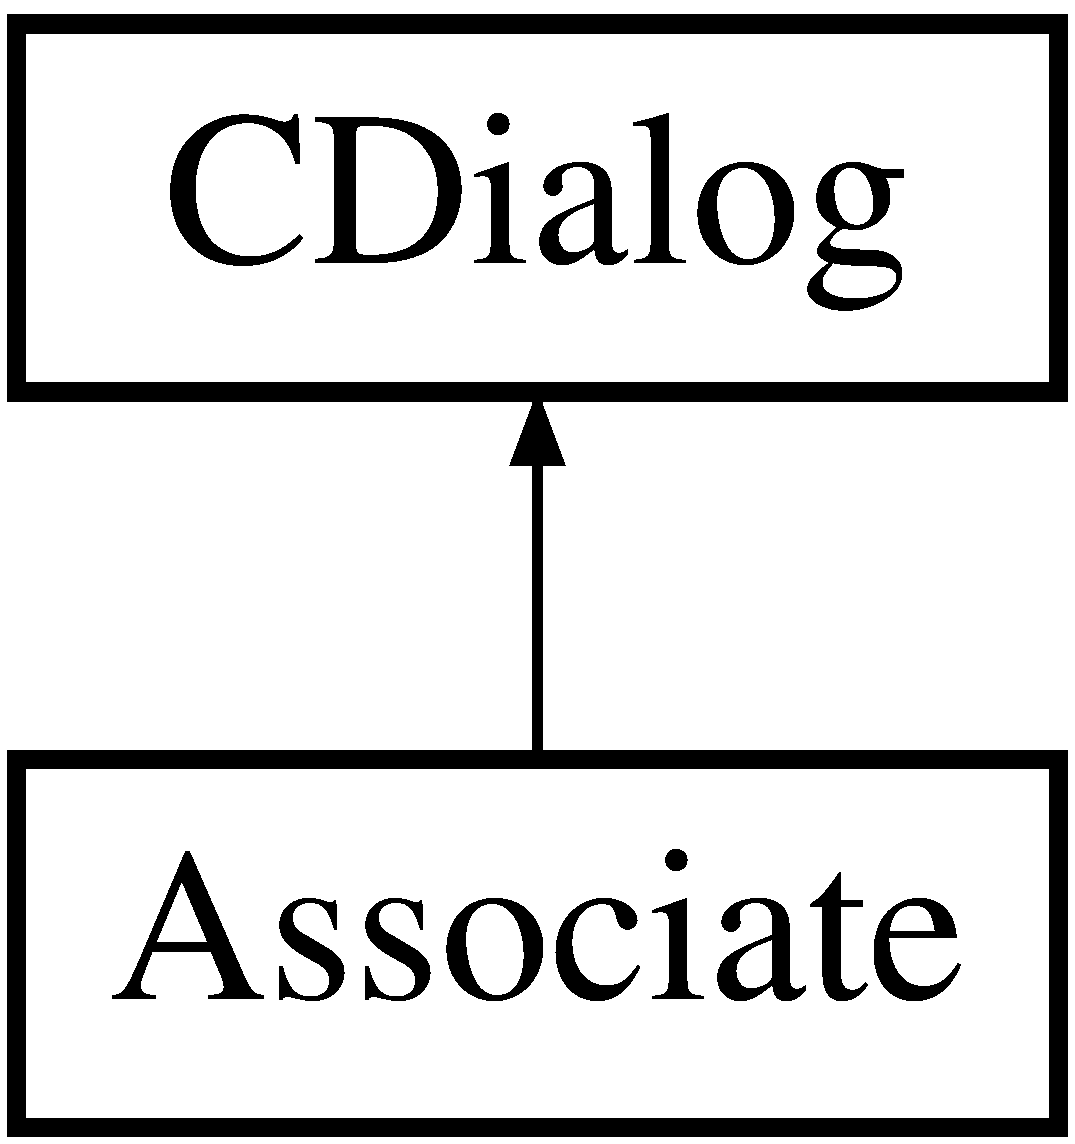
\includegraphics[height=2.000000cm]{class_associate}
\end{center}
\end{figure}
\subsection*{Public 타입}
\begin{DoxyCompactItemize}
\item 
\mbox{\Hypertarget{class_associate_a9696cb7dfd5bf0a5f848d1c0209ca4f8}\label{class_associate_a9696cb7dfd5bf0a5f848d1c0209ca4f8}} 
enum \{ {\bfseries I\+DD} = I\+D\+D\+\_\+\+A\+S\+S\+O\+C\+I\+A\+T\+I\+O\+NS
 \}
\end{DoxyCompactItemize}
\subsection*{Public 멤버 함수}
\begin{DoxyCompactItemize}
\item 
\mbox{\Hypertarget{class_associate_a67a8f8b2f0539a32f8d783f60e2d25b9}\label{class_associate_a67a8f8b2f0539a32f8d783f60e2d25b9}} 
{\bfseries Associate} (C\+Wnd $\ast$p\+Parent=N\+U\+LL)
\end{DoxyCompactItemize}
\subsection*{Public 속성}
\begin{DoxyCompactItemize}
\item 
\mbox{\Hypertarget{class_associate_ab6d59a4b47c5529c1e5f5b8f8b5a6f82}\label{class_associate_ab6d59a4b47c5529c1e5f5b8f8b5a6f82}} 
B\+O\+OL {\bfseries m\+\_\+agb}
\item 
\mbox{\Hypertarget{class_associate_ac132c6bfb6f547702c2e7386650a0a4c}\label{class_associate_ac132c6bfb6f547702c2e7386650a0a4c}} 
B\+O\+OL {\bfseries m\+\_\+bin}
\item 
\mbox{\Hypertarget{class_associate_af245524b613121a7a5291deebfb97e0e}\label{class_associate_af245524b613121a7a5291deebfb97e0e}} 
B\+O\+OL {\bfseries m\+\_\+cgb}
\item 
\mbox{\Hypertarget{class_associate_af4479f05150eb128332d06cba68a955b}\label{class_associate_af4479f05150eb128332d06cba68a955b}} 
B\+O\+OL {\bfseries m\+\_\+gb}
\item 
\mbox{\Hypertarget{class_associate_a7c20c41d1b724e80532ff888b6c7ea56}\label{class_associate_a7c20c41d1b724e80532ff888b6c7ea56}} 
B\+O\+OL {\bfseries m\+\_\+gba}
\item 
\mbox{\Hypertarget{class_associate_a399cc9528f3efc32ec5971fc5e614e97}\label{class_associate_a399cc9528f3efc32ec5971fc5e614e97}} 
B\+O\+OL {\bfseries m\+\_\+gbc}
\item 
\mbox{\Hypertarget{class_associate_a0221f6743a817911817d464579b4a038}\label{class_associate_a0221f6743a817911817d464579b4a038}} 
B\+O\+OL {\bfseries m\+\_\+sgb}
\end{DoxyCompactItemize}
\subsection*{Protected 멤버 함수}
\begin{DoxyCompactItemize}
\item 
\mbox{\Hypertarget{class_associate_af10575d274826cc658ebb2e6a823aa35}\label{class_associate_af10575d274826cc658ebb2e6a823aa35}} 
virtual void {\bfseries Do\+Data\+Exchange} (C\+Data\+Exchange $\ast$p\+DX)
\item 
\mbox{\Hypertarget{class_associate_a66532001ec5d28abd61684b0f62b032b}\label{class_associate_a66532001ec5d28abd61684b0f62b032b}} 
virtual B\+O\+OL {\bfseries On\+Init\+Dialog} ()
\item 
\mbox{\Hypertarget{class_associate_a76fb7e63100511a6d22c53cf3306b8f4}\label{class_associate_a76fb7e63100511a6d22c53cf3306b8f4}} 
afx\+\_\+msg void {\bfseries On\+Cancel} ()
\item 
\mbox{\Hypertarget{class_associate_abb81ded9b91053ed12804ee8674ae860}\label{class_associate_abb81ded9b91053ed12804ee8674ae860}} 
afx\+\_\+msg void {\bfseries On\+Ok} ()
\end{DoxyCompactItemize}


이 클래스에 대한 문서화 페이지는 다음의 파일들로부터 생성되었습니다.\+:\begin{DoxyCompactItemize}
\item 
src/win32/Associate.\+h\item 
src/win32/Associate.\+cpp\end{DoxyCompactItemize}

\hypertarget{class_a_v_i_write}{}\section{A\+V\+I\+Write 클래스 참조}
\label{class_a_v_i_write}\index{A\+V\+I\+Write@{A\+V\+I\+Write}}
\subsection*{Public 멤버 함수}
\begin{DoxyCompactItemize}
\item 
\mbox{\Hypertarget{class_a_v_i_write_a2b4ef2aeeef846bcb12ef58189043eb1}\label{class_a_v_i_write_a2b4ef2aeeef846bcb12ef58189043eb1}} 
bool {\bfseries Open} (const char $\ast$filename)
\item 
\mbox{\Hypertarget{class_a_v_i_write_a904b7f02ff6ecfeeaeec6e1c82f1592a}\label{class_a_v_i_write_a904b7f02ff6ecfeeaeec6e1c82f1592a}} 
virtual bool {\bfseries Add\+Frame} (const int number, const char $\ast$bmp)
\item 
\mbox{\Hypertarget{class_a_v_i_write_a3beb976b918287e0592ab4feebd9ce59}\label{class_a_v_i_write_a3beb976b918287e0592ab4feebd9ce59}} 
void {\bfseries Set\+F\+PS} (int fps)
\item 
\mbox{\Hypertarget{class_a_v_i_write_a1da91adeefacf0dd4655f5029875c5d6}\label{class_a_v_i_write_a1da91adeefacf0dd4655f5029875c5d6}} 
void {\bfseries Set\+Video\+Format} (B\+I\+T\+M\+A\+P\+I\+N\+F\+O\+H\+E\+A\+D\+ER $\ast$)
\item 
\mbox{\Hypertarget{class_a_v_i_write_a7e14c1640c3c888c2b0a0b042c0d5b8f}\label{class_a_v_i_write_a7e14c1640c3c888c2b0a0b042c0d5b8f}} 
bool {\bfseries Is\+Sound\+Added} ()
\item 
\mbox{\Hypertarget{class_a_v_i_write_a8d864e6e2cea4147ffa6f24d69fbe339}\label{class_a_v_i_write_a8d864e6e2cea4147ffa6f24d69fbe339}} 
void {\bfseries Set\+Sound\+Format} (W\+A\+V\+E\+F\+O\+R\+M\+A\+T\+EX $\ast$)
\item 
\mbox{\Hypertarget{class_a_v_i_write_a63b7d54c048e517bbfad0ae2004d9861}\label{class_a_v_i_write_a63b7d54c048e517bbfad0ae2004d9861}} 
bool {\bfseries Add\+Sound} (const char $\ast$sound, int len)
\end{DoxyCompactItemize}


이 클래스에 대한 문서화 페이지는 다음의 파일들로부터 생성되었습니다.\+:\begin{DoxyCompactItemize}
\item 
src/win32/A\+V\+I\+Write.\+h\item 
src/win32/A\+V\+I\+Write.\+cpp\end{DoxyCompactItemize}

\hypertarget{class_bitmap_control}{}\section{Bitmap\+Control 클래스 참조}
\label{class_bitmap_control}\index{Bitmap\+Control@{Bitmap\+Control}}
Bitmap\+Control에 대한 상속 다이어그램 \+: \begin{figure}[H]
\begin{center}
\leavevmode
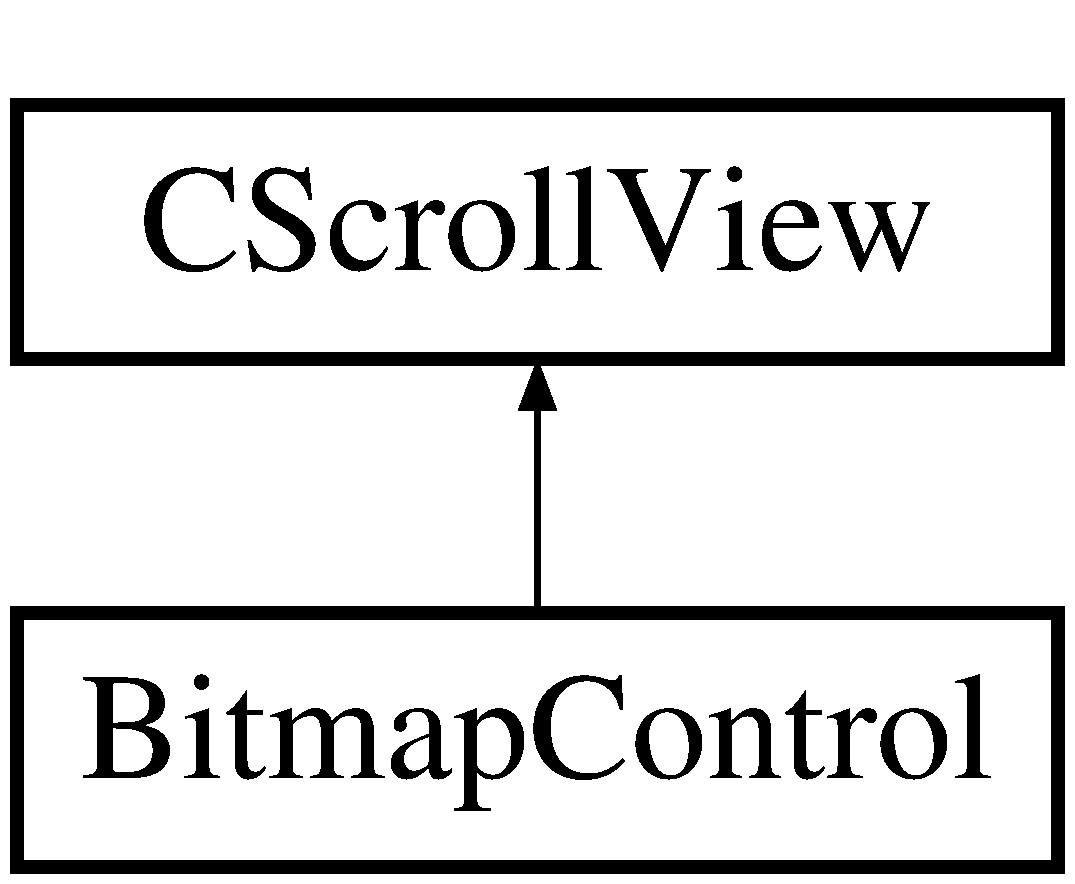
\includegraphics[height=2.000000cm]{class_bitmap_control}
\end{center}
\end{figure}
\subsection*{Public 멤버 함수}
\begin{DoxyCompactItemize}
\item 
\mbox{\Hypertarget{class_bitmap_control_ab545e15ea3edda9f0d80c0b8b0b7c812}\label{class_bitmap_control_ab545e15ea3edda9f0d80c0b8b0b7c812}} 
void {\bfseries set\+Stretch} (bool b)
\item 
\mbox{\Hypertarget{class_bitmap_control_acf061a1e9a4cad90ad2827c14f79caa2}\label{class_bitmap_control_acf061a1e9a4cad90ad2827c14f79caa2}} 
void {\bfseries refresh} ()
\item 
\mbox{\Hypertarget{class_bitmap_control_a421004fe6ba01329dd69259396592d1f}\label{class_bitmap_control_a421004fe6ba01329dd69259396592d1f}} 
void {\bfseries set\+Size} (int w1, int h1)
\item 
\mbox{\Hypertarget{class_bitmap_control_aa6206183896caf192a37709fa5d7b8d2}\label{class_bitmap_control_aa6206183896caf192a37709fa5d7b8d2}} 
void {\bfseries set\+Data} (u8 $\ast$d)
\item 
\mbox{\Hypertarget{class_bitmap_control_a301c52fc62de4368fccdcdc93cefad0b}\label{class_bitmap_control_a301c52fc62de4368fccdcdc93cefad0b}} 
void {\bfseries set\+Bmp\+Info} (B\+I\+T\+M\+A\+P\+I\+N\+FO $\ast$info)
\item 
\mbox{\Hypertarget{class_bitmap_control_a1d3cff9a3b57dd7558d678177dcf4b5c}\label{class_bitmap_control_a1d3cff9a3b57dd7558d678177dcf4b5c}} 
bool {\bfseries get\+Stretch} ()
\end{DoxyCompactItemize}
\subsection*{정적 Public 속성}
\begin{DoxyCompactItemize}
\item 
\mbox{\Hypertarget{class_bitmap_control_acd16ac02d48f1201fc90470b6e29c7fe}\label{class_bitmap_control_acd16ac02d48f1201fc90470b6e29c7fe}} 
static bool {\bfseries is\+Registered} = false
\end{DoxyCompactItemize}
\subsection*{Protected 멤버 함수}
\begin{DoxyCompactItemize}
\item 
\mbox{\Hypertarget{class_bitmap_control_a76ead24c70d33421148716a39cf3a17f}\label{class_bitmap_control_a76ead24c70d33421148716a39cf3a17f}} 
virtual void {\bfseries On\+Draw} (C\+DC $\ast$p\+DC)
\item 
\mbox{\Hypertarget{class_bitmap_control_a532fd9e0bd31674589a224737960bfc0}\label{class_bitmap_control_a532fd9e0bd31674589a224737960bfc0}} 
virtual void {\bfseries On\+Initial\+Update} ()
\item 
\mbox{\Hypertarget{class_bitmap_control_aed7e031df3fd65a4325ea9bf7da5bdc3}\label{class_bitmap_control_aed7e031df3fd65a4325ea9bf7da5bdc3}} 
virtual void {\bfseries Post\+Nc\+Destroy} ()
\item 
\mbox{\Hypertarget{class_bitmap_control_aea73d6e790bb4828eb230c3cd66e5e0b}\label{class_bitmap_control_aea73d6e790bb4828eb230c3cd66e5e0b}} 
afx\+\_\+msg B\+O\+OL {\bfseries On\+Erase\+Bkgnd} (C\+DC $\ast$p\+DC)
\item 
\mbox{\Hypertarget{class_bitmap_control_ac0e60f98809d78a38d5d35942c1bfb2c}\label{class_bitmap_control_ac0e60f98809d78a38d5d35942c1bfb2c}} 
afx\+\_\+msg void {\bfseries On\+Size} (U\+I\+NT n\+Type, int cx, int cy)
\item 
\mbox{\Hypertarget{class_bitmap_control_a2958d0209f702d4207d10797c8aa86bd}\label{class_bitmap_control_a2958d0209f702d4207d10797c8aa86bd}} 
afx\+\_\+msg void {\bfseries On\+L\+Button\+Down} (U\+I\+NT n\+Flags, C\+Point point)
\end{DoxyCompactItemize}


이 클래스에 대한 문서화 페이지는 다음의 파일들로부터 생성되었습니다.\+:\begin{DoxyCompactItemize}
\item 
src/win32/Bitmap\+Control.\+h\item 
src/win32/Bitmap\+Control.\+cpp\end{DoxyCompactItemize}

\hypertarget{structbreakpoint_info}{}\section{breakpoint\+Info 구조체 참조}
\label{structbreakpoint_info}\index{breakpoint\+Info@{breakpoint\+Info}}


breakpoint\+Info에 대한 협력 다이어그램\+:\nopagebreak
\begin{figure}[H]
\begin{center}
\leavevmode
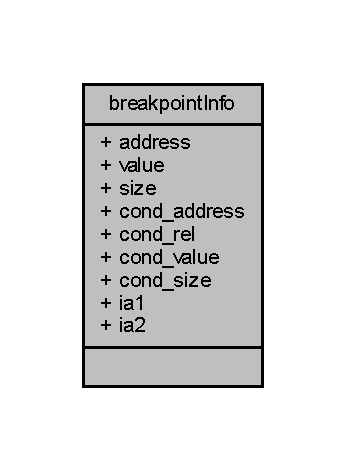
\includegraphics[width=166pt]{structbreakpoint_info__coll__graph}
\end{center}
\end{figure}
\subsection*{Public 속성}
\begin{DoxyCompactItemize}
\item 
\mbox{\hyperlink{_system_8h_a10e94b422ef0c20dcdec20d31a1f5049}{u32}} \mbox{\hyperlink{structbreakpoint_info_ab0cc4bdc931703296ec18aaa1e2242f4}{address}}
\item 
\mbox{\hyperlink{_system_8h_a10e94b422ef0c20dcdec20d31a1f5049}{u32}} \mbox{\hyperlink{structbreakpoint_info_a10cf821e6c0c5b11b921baafa0144448}{value}}
\item 
\mbox{\hyperlink{_util_8cpp_a0ef32aa8672df19503a49fab2d0c8071}{int}} \mbox{\hyperlink{structbreakpoint_info_a39a2c2fabe9c630917e8131a99ce61ec}{size}}
\item 
\mbox{\hyperlink{_system_8h_a10e94b422ef0c20dcdec20d31a1f5049}{u32}} \mbox{\hyperlink{structbreakpoint_info_a4a83f60b18f30afe9fa114b21f02de22}{cond\+\_\+address}}
\item 
char \mbox{\hyperlink{structbreakpoint_info_a6819ea8a99055196410b1070f9750f70}{cond\+\_\+rel}}
\item 
\mbox{\hyperlink{_system_8h_a10e94b422ef0c20dcdec20d31a1f5049}{u32}} \mbox{\hyperlink{structbreakpoint_info_a06f4bafc5e974ae0adf0e3bf651d2afd}{cond\+\_\+value}}
\item 
\mbox{\hyperlink{_util_8cpp_a0ef32aa8672df19503a49fab2d0c8071}{int}} \mbox{\hyperlink{structbreakpoint_info_a4c2f4f1b0f74562121d829e864d73a0e}{cond\+\_\+size}}
\item 
bool \mbox{\hyperlink{structbreakpoint_info_a6d1174b3ac7266b9454683ee36030b97}{ia1}}
\item 
bool \mbox{\hyperlink{structbreakpoint_info_a5c43894b7302cbb085204b39a14dda91}{ia2}}
\end{DoxyCompactItemize}


\subsection{상세한 설명}


debugger.\+cpp 파일의 57 번째 라인에서 정의되었습니다.



\subsection{멤버 데이터 문서화}
\mbox{\Hypertarget{structbreakpoint_info_ab0cc4bdc931703296ec18aaa1e2242f4}\label{structbreakpoint_info_ab0cc4bdc931703296ec18aaa1e2242f4}} 
\index{breakpoint\+Info@{breakpoint\+Info}!address@{address}}
\index{address@{address}!breakpoint\+Info@{breakpoint\+Info}}
\subsubsection{\texorpdfstring{address}{address}}
{\footnotesize\ttfamily \mbox{\hyperlink{_system_8h_a10e94b422ef0c20dcdec20d31a1f5049}{u32}} breakpoint\+Info\+::address}



debugger.\+cpp 파일의 58 번째 라인에서 정의되었습니다.

\mbox{\Hypertarget{structbreakpoint_info_a4a83f60b18f30afe9fa114b21f02de22}\label{structbreakpoint_info_a4a83f60b18f30afe9fa114b21f02de22}} 
\index{breakpoint\+Info@{breakpoint\+Info}!cond\+\_\+address@{cond\+\_\+address}}
\index{cond\+\_\+address@{cond\+\_\+address}!breakpoint\+Info@{breakpoint\+Info}}
\subsubsection{\texorpdfstring{cond\+\_\+address}{cond\_address}}
{\footnotesize\ttfamily \mbox{\hyperlink{_system_8h_a10e94b422ef0c20dcdec20d31a1f5049}{u32}} breakpoint\+Info\+::cond\+\_\+address}



debugger.\+cpp 파일의 62 번째 라인에서 정의되었습니다.

\mbox{\Hypertarget{structbreakpoint_info_a6819ea8a99055196410b1070f9750f70}\label{structbreakpoint_info_a6819ea8a99055196410b1070f9750f70}} 
\index{breakpoint\+Info@{breakpoint\+Info}!cond\+\_\+rel@{cond\+\_\+rel}}
\index{cond\+\_\+rel@{cond\+\_\+rel}!breakpoint\+Info@{breakpoint\+Info}}
\subsubsection{\texorpdfstring{cond\+\_\+rel}{cond\_rel}}
{\footnotesize\ttfamily char breakpoint\+Info\+::cond\+\_\+rel}



debugger.\+cpp 파일의 63 번째 라인에서 정의되었습니다.

\mbox{\Hypertarget{structbreakpoint_info_a4c2f4f1b0f74562121d829e864d73a0e}\label{structbreakpoint_info_a4c2f4f1b0f74562121d829e864d73a0e}} 
\index{breakpoint\+Info@{breakpoint\+Info}!cond\+\_\+size@{cond\+\_\+size}}
\index{cond\+\_\+size@{cond\+\_\+size}!breakpoint\+Info@{breakpoint\+Info}}
\subsubsection{\texorpdfstring{cond\+\_\+size}{cond\_size}}
{\footnotesize\ttfamily \mbox{\hyperlink{_util_8cpp_a0ef32aa8672df19503a49fab2d0c8071}{int}} breakpoint\+Info\+::cond\+\_\+size}



debugger.\+cpp 파일의 65 번째 라인에서 정의되었습니다.

\mbox{\Hypertarget{structbreakpoint_info_a06f4bafc5e974ae0adf0e3bf651d2afd}\label{structbreakpoint_info_a06f4bafc5e974ae0adf0e3bf651d2afd}} 
\index{breakpoint\+Info@{breakpoint\+Info}!cond\+\_\+value@{cond\+\_\+value}}
\index{cond\+\_\+value@{cond\+\_\+value}!breakpoint\+Info@{breakpoint\+Info}}
\subsubsection{\texorpdfstring{cond\+\_\+value}{cond\_value}}
{\footnotesize\ttfamily \mbox{\hyperlink{_system_8h_a10e94b422ef0c20dcdec20d31a1f5049}{u32}} breakpoint\+Info\+::cond\+\_\+value}



debugger.\+cpp 파일의 64 번째 라인에서 정의되었습니다.

\mbox{\Hypertarget{structbreakpoint_info_a6d1174b3ac7266b9454683ee36030b97}\label{structbreakpoint_info_a6d1174b3ac7266b9454683ee36030b97}} 
\index{breakpoint\+Info@{breakpoint\+Info}!ia1@{ia1}}
\index{ia1@{ia1}!breakpoint\+Info@{breakpoint\+Info}}
\subsubsection{\texorpdfstring{ia1}{ia1}}
{\footnotesize\ttfamily bool breakpoint\+Info\+::ia1}



debugger.\+cpp 파일의 66 번째 라인에서 정의되었습니다.

\mbox{\Hypertarget{structbreakpoint_info_a5c43894b7302cbb085204b39a14dda91}\label{structbreakpoint_info_a5c43894b7302cbb085204b39a14dda91}} 
\index{breakpoint\+Info@{breakpoint\+Info}!ia2@{ia2}}
\index{ia2@{ia2}!breakpoint\+Info@{breakpoint\+Info}}
\subsubsection{\texorpdfstring{ia2}{ia2}}
{\footnotesize\ttfamily bool breakpoint\+Info\+::ia2}



debugger.\+cpp 파일의 67 번째 라인에서 정의되었습니다.

\mbox{\Hypertarget{structbreakpoint_info_a39a2c2fabe9c630917e8131a99ce61ec}\label{structbreakpoint_info_a39a2c2fabe9c630917e8131a99ce61ec}} 
\index{breakpoint\+Info@{breakpoint\+Info}!size@{size}}
\index{size@{size}!breakpoint\+Info@{breakpoint\+Info}}
\subsubsection{\texorpdfstring{size}{size}}
{\footnotesize\ttfamily \mbox{\hyperlink{_util_8cpp_a0ef32aa8672df19503a49fab2d0c8071}{int}} breakpoint\+Info\+::size}



debugger.\+cpp 파일의 60 번째 라인에서 정의되었습니다.

\mbox{\Hypertarget{structbreakpoint_info_a10cf821e6c0c5b11b921baafa0144448}\label{structbreakpoint_info_a10cf821e6c0c5b11b921baafa0144448}} 
\index{breakpoint\+Info@{breakpoint\+Info}!value@{value}}
\index{value@{value}!breakpoint\+Info@{breakpoint\+Info}}
\subsubsection{\texorpdfstring{value}{value}}
{\footnotesize\ttfamily \mbox{\hyperlink{_system_8h_a10e94b422ef0c20dcdec20d31a1f5049}{u32}} breakpoint\+Info\+::value}



debugger.\+cpp 파일의 59 번째 라인에서 정의되었습니다.



이 구조체에 대한 문서화 페이지는 다음의 파일로부터 생성되었습니다.\+:\begin{DoxyCompactItemize}
\item 
C\+:/\+Users/sjh13/sources/\+Visual\+Boy\+Advance/src/sdl/\mbox{\hyperlink{debugger_8cpp}{debugger.\+cpp}}\end{DoxyCompactItemize}

\hypertarget{class_bug_report}{}\section{Bug\+Report 클래스 참조}
\label{class_bug_report}\index{Bug\+Report@{Bug\+Report}}
Bug\+Report에 대한 상속 다이어그램 \+: \begin{figure}[H]
\begin{center}
\leavevmode
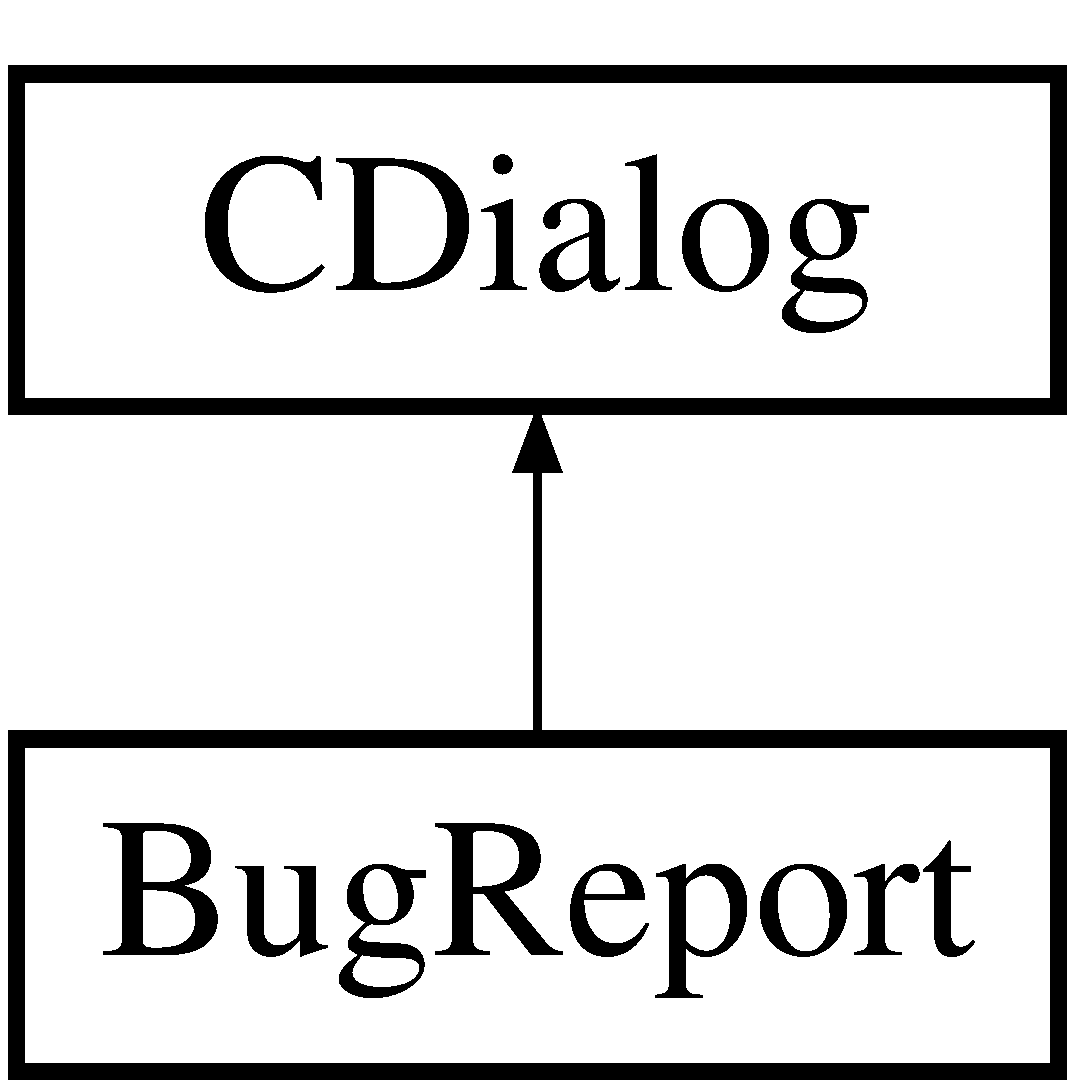
\includegraphics[height=2.000000cm]{class_bug_report}
\end{center}
\end{figure}
\subsection*{Public 타입}
\begin{DoxyCompactItemize}
\item 
\mbox{\Hypertarget{class_bug_report_ac5c6f1960b86db3b70eab6b21625913e}\label{class_bug_report_ac5c6f1960b86db3b70eab6b21625913e}} 
enum \{ {\bfseries I\+DD} = I\+D\+D\+\_\+\+B\+U\+G\+\_\+\+R\+E\+P\+O\+RT
 \}
\end{DoxyCompactItemize}
\subsection*{Public 멤버 함수}
\begin{DoxyCompactItemize}
\item 
\mbox{\Hypertarget{class_bug_report_a0b78ee082b1ca2a2a2c16db3d65842fb}\label{class_bug_report_a0b78ee082b1ca2a2a2c16db3d65842fb}} 
{\bfseries Bug\+Report} (C\+Wnd $\ast$p\+Parent=N\+U\+LL)
\end{DoxyCompactItemize}
\subsection*{Public 속성}
\begin{DoxyCompactItemize}
\item 
\mbox{\Hypertarget{class_bug_report_aef6dd887fcfe40d98d0fa1c6cf2d2466}\label{class_bug_report_aef6dd887fcfe40d98d0fa1c6cf2d2466}} 
C\+Edit {\bfseries m\+\_\+report}
\end{DoxyCompactItemize}
\subsection*{Protected 멤버 함수}
\begin{DoxyCompactItemize}
\item 
\mbox{\Hypertarget{class_bug_report_a5b019306aeca9497b7b6efd438a44558}\label{class_bug_report_a5b019306aeca9497b7b6efd438a44558}} 
virtual void {\bfseries Do\+Data\+Exchange} (C\+Data\+Exchange $\ast$p\+DX)
\item 
\mbox{\Hypertarget{class_bug_report_afe00e8dd3efa190199d8d645cb702e07}\label{class_bug_report_afe00e8dd3efa190199d8d645cb702e07}} 
C\+String {\bfseries create\+Report} ()
\item 
\mbox{\Hypertarget{class_bug_report_a6b74689c7cf7ed6daeaaf2dc8f1498ab}\label{class_bug_report_a6b74689c7cf7ed6daeaaf2dc8f1498ab}} 
afx\+\_\+msg void {\bfseries On\+Copy} ()
\item 
\mbox{\Hypertarget{class_bug_report_a2c9a7f1da33a46ca97f0ecd821e701e9}\label{class_bug_report_a2c9a7f1da33a46ca97f0ecd821e701e9}} 
afx\+\_\+msg void {\bfseries On\+Ok} ()
\item 
\mbox{\Hypertarget{class_bug_report_abcfc2e192747272d1708a1d479bfd45b}\label{class_bug_report_abcfc2e192747272d1708a1d479bfd45b}} 
virtual B\+O\+OL {\bfseries On\+Init\+Dialog} ()
\end{DoxyCompactItemize}


이 클래스에 대한 문서화 페이지는 다음의 파일들로부터 생성되었습니다.\+:\begin{DoxyCompactItemize}
\item 
src/win32/Bug\+Report.\+h\item 
src/win32/Bug\+Report.\+cpp\end{DoxyCompactItemize}

\hypertarget{class_c_accelerator_manager}{}\section{C\+Accelerator\+Manager 클래스 참조}
\label{class_c_accelerator_manager}\index{C\+Accelerator\+Manager@{C\+Accelerator\+Manager}}
C\+Accelerator\+Manager에 대한 상속 다이어그램 \+: \begin{figure}[H]
\begin{center}
\leavevmode
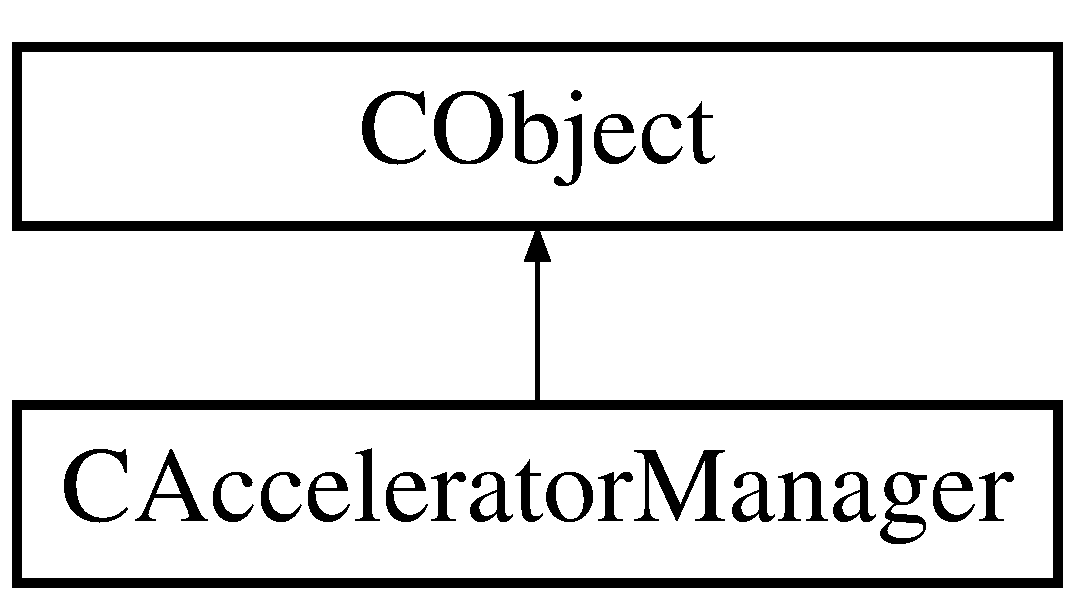
\includegraphics[height=2.000000cm]{class_c_accelerator_manager}
\end{center}
\end{figure}
\subsection*{Public 멤버 함수}
\begin{DoxyCompactItemize}
\item 
\mbox{\Hypertarget{class_c_accelerator_manager_ac7411d20f413ea0ec3bd65705b564adf}\label{class_c_accelerator_manager_ac7411d20f413ea0ec3bd65705b564adf}} 
void {\bfseries Update\+Menu} (H\+M\+E\+NU menu)
\item 
\mbox{\Hypertarget{class_c_accelerator_manager_ac854ec5263a7bab961bf63aec3938984}\label{class_c_accelerator_manager_ac854ec5263a7bab961bf63aec3938984}} 
void {\bfseries Update\+Menu} ()
\item 
\mbox{\Hypertarget{class_c_accelerator_manager_a2d01e04665e3d03f3c1410bd69b0a82c}\label{class_c_accelerator_manager_a2d01e04665e3d03f3c1410bd69b0a82c}} 
void {\bfseries Connect} (C\+Wnd $\ast$p\+Wnd, bool b\+Auto\+Save=true)
\item 
\mbox{\Hypertarget{class_c_accelerator_manager_a8e87ae6f5464a4fa052c91c0ee361b6d}\label{class_c_accelerator_manager_a8e87ae6f5464a4fa052c91c0ee361b6d}} 
bool {\bfseries Load} (H\+K\+EY h\+Reg\+Key, L\+P\+C\+T\+S\+TR sz\+Reg\+Key)
\item 
\mbox{\Hypertarget{class_c_accelerator_manager_a289a9052abea7302d9322283f93cbce6}\label{class_c_accelerator_manager_a289a9052abea7302d9322283f93cbce6}} 
bool {\bfseries Load} ()
\item 
\mbox{\Hypertarget{class_c_accelerator_manager_a6ddd05a54ab0e66bc6ca8a7af3742e61}\label{class_c_accelerator_manager_a6ddd05a54ab0e66bc6ca8a7af3742e61}} 
bool {\bfseries Write} ()
\item 
\mbox{\Hypertarget{class_c_accelerator_manager_aa510a36964ed209de5f7325efa713bf6}\label{class_c_accelerator_manager_aa510a36964ed209de5f7325efa713bf6}} 
bool {\bfseries Default} ()
\item 
\mbox{\Hypertarget{class_c_accelerator_manager_aaefac809b336df14e1a1a7d60f72ae28}\label{class_c_accelerator_manager_aaefac809b336df14e1a1a7d60f72ae28}} 
bool {\bfseries Create\+Default\+Table} ()
\item 
\mbox{\Hypertarget{class_c_accelerator_manager_a508e56037762d035758491d12fd10dfa}\label{class_c_accelerator_manager_a508e56037762d035758491d12fd10dfa}} 
bool {\bfseries Is\+Default\+Table\+Available} ()
\item 
\mbox{\Hypertarget{class_c_accelerator_manager_a6773f028b9c0b04c9a7b6d02c1a96be0}\label{class_c_accelerator_manager_a6773f028b9c0b04c9a7b6d02c1a96be0}} 
bool {\bfseries Is\+Map\+String\+Commands\+Empty} ()
\item 
\mbox{\Hypertarget{class_c_accelerator_manager_afcb43e85351bae0fb475dac40ba4cede}\label{class_c_accelerator_manager_afcb43e85351bae0fb475dac40ba4cede}} 
bool {\bfseries Get\+Reg\+Key} (H\+K\+EY \&h\+Reg\+Key, C\+String \&sz\+Reg\+Key)
\item 
\mbox{\Hypertarget{class_c_accelerator_manager_a6ea67e9b2bfbda2f0305024e0d73a5bb}\label{class_c_accelerator_manager_a6ea67e9b2bfbda2f0305024e0d73a5bb}} 
bool {\bfseries Set\+Reg\+Key} (H\+K\+EY h\+Reg\+Key, L\+P\+C\+T\+S\+TR sz\+Reg\+Key)
\item 
\mbox{\Hypertarget{class_c_accelerator_manager_a895420283e3ce58576ded1a3f999724a}\label{class_c_accelerator_manager_a895420283e3ce58576ded1a3f999724a}} 
bool {\bfseries Is\+Auto\+Save} ()
\item 
\mbox{\Hypertarget{class_c_accelerator_manager_a84b4a9dfb4afc48430655e234ff94349}\label{class_c_accelerator_manager_a84b4a9dfb4afc48430655e234ff94349}} 
void {\bfseries Set\+Auto\+Save} (bool b\+Auto\+Save)
\item 
\mbox{\Hypertarget{class_c_accelerator_manager_a5e861b03f3647e8c4998c49ccd4d8928}\label{class_c_accelerator_manager_a5e861b03f3647e8c4998c49ccd4d8928}} 
bool {\bfseries Get\+String\+From\+A\+C\+C\+EL} (A\+C\+C\+EL $\ast$p\+A\+C\+C\+EL, C\+String \&sz\+Accel)
\item 
\mbox{\Hypertarget{class_c_accelerator_manager_adf91477de6b9df320930786c9755b0eb}\label{class_c_accelerator_manager_adf91477de6b9df320930786c9755b0eb}} 
bool {\bfseries Get\+String\+From\+A\+C\+C\+EL} (B\+Y\+TE c\+Virt, W\+O\+RD n\+Code, C\+String \&sz\+Accel)
\item 
\mbox{\Hypertarget{class_c_accelerator_manager_a3fa9c8e4f44acc76cc40fc7382e597d8}\label{class_c_accelerator_manager_a3fa9c8e4f44acc76cc40fc7382e597d8}} 
bool {\bfseries Update\+Wnd\+Table} ()
\item 
\mbox{\Hypertarget{class_c_accelerator_manager_a96957fd8ed0a15d0dbc508359824db3c}\label{class_c_accelerator_manager_a96957fd8ed0a15d0dbc508359824db3c}} 
bool {\bfseries Set\+Accel} (B\+Y\+TE c\+Virt, W\+O\+RD w\+I\+D\+Command, W\+O\+RD w\+New\+Caract, L\+P\+C\+T\+S\+TR sz\+Command, bool b\+Locked=false)
\item 
\mbox{\Hypertarget{class_c_accelerator_manager_a05227e733c2c5d4a4d8074bf28a4f333}\label{class_c_accelerator_manager_a05227e733c2c5d4a4d8074bf28a4f333}} 
bool {\bfseries Add\+Command\+Accel} (W\+O\+RD w\+I\+D\+Command, L\+P\+C\+T\+S\+TR sz\+Command, bool b\+Locked=true)
\item 
\mbox{\Hypertarget{class_c_accelerator_manager_ab534c2d8c0d7d7e30c5e907677bfad68}\label{class_c_accelerator_manager_ab534c2d8c0d7d7e30c5e907677bfad68}} 
bool {\bfseries Create\+Entry} (W\+O\+RD w\+I\+D\+Command, L\+P\+C\+T\+S\+TR sz\+Command)
\item 
\mbox{\Hypertarget{class_c_accelerator_manager_ae20cd0e0259b70fe7443b442e85d1213}\label{class_c_accelerator_manager_ae20cd0e0259b70fe7443b442e85d1213}} 
bool {\bfseries Delete\+Entry} (L\+P\+C\+T\+S\+TR sz\+Command)
\item 
\mbox{\Hypertarget{class_c_accelerator_manager_a25f2470050bd966a2f45235381dda32b}\label{class_c_accelerator_manager_a25f2470050bd966a2f45235381dda32b}} 
bool {\bfseries Delete\+Entry} (W\+O\+RD w\+I\+D\+Command)
\item 
\mbox{\Hypertarget{class_c_accelerator_manager_a73426e98a7fb4d8e5481a8e55a8a2626}\label{class_c_accelerator_manager_a73426e98a7fb4d8e5481a8e55a8a2626}} 
bool {\bfseries Delete\+Accel} (B\+Y\+TE c\+Virt, W\+O\+RD w\+I\+D\+Command, W\+O\+RD w\+New\+Caract)
\item 
\mbox{\Hypertarget{class_c_accelerator_manager_a11c56cbcdfac0008ecb4aef10ba51ae8}\label{class_c_accelerator_manager_a11c56cbcdfac0008ecb4aef10ba51ae8}} 
\mbox{\hyperlink{class_c_accelerator_manager}{C\+Accelerator\+Manager}} \& {\bfseries operator=} (const \mbox{\hyperlink{class_c_accelerator_manager}{C\+Accelerator\+Manager}} \&accelmgr)
\end{DoxyCompactItemize}
\subsection*{Protected 멤버 함수}
\begin{DoxyCompactItemize}
\item 
\mbox{\Hypertarget{class_c_accelerator_manager_aca456cda1a5f9b17bcfaea4f8ff45903}\label{class_c_accelerator_manager_aca456cda1a5f9b17bcfaea4f8ff45903}} 
void {\bfseries Reset} ()
\item 
\mbox{\Hypertarget{class_c_accelerator_manager_ac9e0e988625c9687666a9f582f9b3536}\label{class_c_accelerator_manager_ac9e0e988625c9687666a9f582f9b3536}} 
bool {\bfseries Add\+Accel} (B\+Y\+TE c\+Virt, W\+O\+RD w\+I\+D\+Command, W\+O\+RD w\+Key, L\+P\+C\+T\+S\+TR sz\+Command, bool b\+Locked)
\end{DoxyCompactItemize}
\subsection*{Protected 속성}
\begin{DoxyCompactItemize}
\item 
\mbox{\Hypertarget{class_c_accelerator_manager_a24f706c75f754982051e1d7fad1916da}\label{class_c_accelerator_manager_a24f706c75f754982051e1d7fad1916da}} 
C\+Wnd $\ast$ {\bfseries m\+\_\+p\+Wnd\+Connected}
\item 
\mbox{\Hypertarget{class_c_accelerator_manager_abb40dbb1a44c47ac22590e8f1243835b}\label{class_c_accelerator_manager_abb40dbb1a44c47ac22590e8f1243835b}} 
C\+Map\+String\+To\+Word {\bfseries m\+\_\+map\+Accel\+String}
\item 
\mbox{\Hypertarget{class_c_accelerator_manager_a16b8d3e9328bc0eeeb048630deff2768}\label{class_c_accelerator_manager_a16b8d3e9328bc0eeeb048630deff2768}} 
C\+Map\+Word\+To\+C\+Cmd\+Accel\+Ob {\bfseries m\+\_\+map\+Accel\+Table}
\item 
\mbox{\Hypertarget{class_c_accelerator_manager_ad7c3ac9a16b8f19e0b5524d8582a5fae}\label{class_c_accelerator_manager_ad7c3ac9a16b8f19e0b5524d8582a5fae}} 
C\+Map\+Word\+To\+C\+Cmd\+Accel\+Ob {\bfseries m\+\_\+map\+Accel\+Table\+Saved}
\item 
\mbox{\Hypertarget{class_c_accelerator_manager_ac563baf2a7cedb91bc44e9b8581a6020}\label{class_c_accelerator_manager_ac563baf2a7cedb91bc44e9b8581a6020}} 
bool {\bfseries m\+\_\+b\+Default\+Table}
\item 
\mbox{\Hypertarget{class_c_accelerator_manager_a2652d64c947f7f3474b3aa054861b34b}\label{class_c_accelerator_manager_a2652d64c947f7f3474b3aa054861b34b}} 
H\+K\+EY {\bfseries m\+\_\+h\+Reg\+Key}
\item 
\mbox{\Hypertarget{class_c_accelerator_manager_a03a6d0e43bcfb63cf1a23ad12cb5aa35}\label{class_c_accelerator_manager_a03a6d0e43bcfb63cf1a23ad12cb5aa35}} 
C\+String {\bfseries m\+\_\+sz\+Reg\+Key}
\item 
\mbox{\Hypertarget{class_c_accelerator_manager_a37b504c74c13ca2d62eea8abffe73102}\label{class_c_accelerator_manager_a37b504c74c13ca2d62eea8abffe73102}} 
bool {\bfseries m\+\_\+b\+Auto\+Save}
\end{DoxyCompactItemize}
\subsection*{Friends}
\begin{DoxyCompactItemize}
\item 
\mbox{\Hypertarget{class_c_accelerator_manager_ad13d9a415d0447ece033ae132991aefc}\label{class_c_accelerator_manager_ad13d9a415d0447ece033ae132991aefc}} 
class {\bfseries Accel\+Editor}
\end{DoxyCompactItemize}


이 클래스에 대한 문서화 페이지는 다음의 파일들로부터 생성되었습니다.\+:\begin{DoxyCompactItemize}
\item 
src/win32/Accelerator\+Manager.\+h\item 
src/win32/Accelerator\+Manager.\+cpp\end{DoxyCompactItemize}

\hypertarget{class_c_accels_ob}{}\section{C\+Accels\+Ob 클래스 참조}
\label{class_c_accels_ob}\index{C\+Accels\+Ob@{C\+Accels\+Ob}}
C\+Accels\+Ob에 대한 상속 다이어그램 \+: \begin{figure}[H]
\begin{center}
\leavevmode
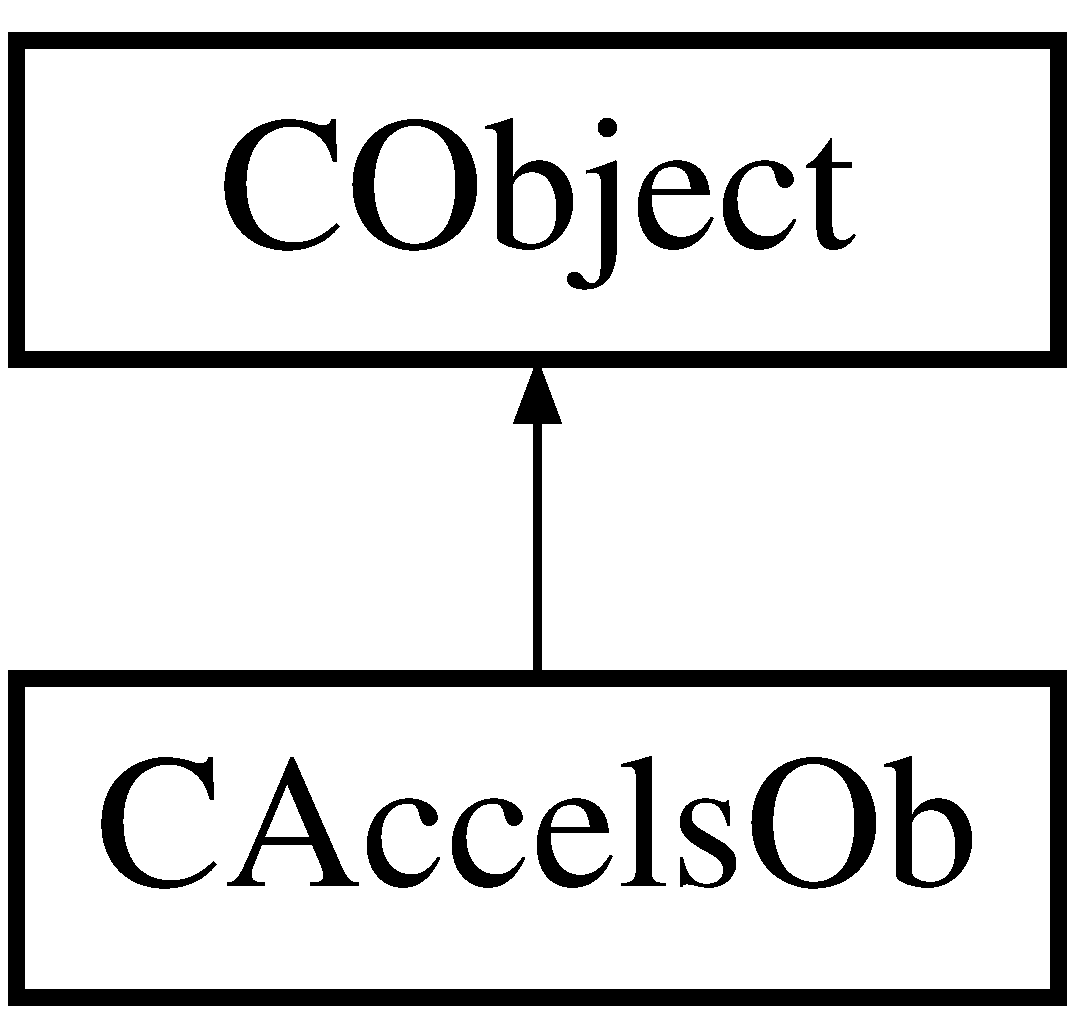
\includegraphics[height=2.000000cm]{class_c_accels_ob}
\end{center}
\end{figure}
\subsection*{Public 멤버 함수}
\begin{DoxyCompactItemize}
\item 
\mbox{\Hypertarget{class_c_accels_ob_afca345908aafde57de46430bbf2018d9}\label{class_c_accels_ob_afca345908aafde57de46430bbf2018d9}} 
{\bfseries C\+Accels\+Ob} (\mbox{\hyperlink{class_c_accels_ob}{C\+Accels\+Ob}} $\ast$p\+From)
\item 
\mbox{\Hypertarget{class_c_accels_ob_acba35eec2e75114289468292870bf484}\label{class_c_accels_ob_acba35eec2e75114289468292870bf484}} 
{\bfseries C\+Accels\+Ob} (B\+Y\+TE c\+Virt, W\+O\+RD w\+Key, bool b\+Locked=false)
\item 
\mbox{\Hypertarget{class_c_accels_ob_aa28d7238be643bb20d922cb360881bd6}\label{class_c_accels_ob_aa28d7238be643bb20d922cb360881bd6}} 
{\bfseries C\+Accels\+Ob} (L\+P\+A\+C\+C\+EL p\+A\+C\+C\+EL)
\item 
\mbox{\Hypertarget{class_c_accels_ob_ae6075be9ad7656823f5cecd277dd7d6e}\label{class_c_accels_ob_ae6075be9ad7656823f5cecd277dd7d6e}} 
\mbox{\hyperlink{class_c_accels_ob}{C\+Accels\+Ob}} \& {\bfseries operator=} (const \mbox{\hyperlink{class_c_accels_ob}{C\+Accels\+Ob}} \&from)
\item 
\mbox{\Hypertarget{class_c_accels_ob_afaf7510fa1e0707863f6bd469f190de6}\label{class_c_accels_ob_afaf7510fa1e0707863f6bd469f190de6}} 
void {\bfseries Get\+String} (C\+String \&sz\+Buffer)
\item 
\mbox{\Hypertarget{class_c_accels_ob_a32714a4454d398d3d3a68d1705a76bc5}\label{class_c_accels_ob_a32714a4454d398d3d3a68d1705a76bc5}} 
bool {\bfseries Is\+Equal} (W\+O\+RD w\+Key, bool b\+Ctrl, bool b\+Alt, bool b\+Shift)
\item 
\mbox{\Hypertarget{class_c_accels_ob_abbbdc5e93061f67ade785c9e4f07b918}\label{class_c_accels_ob_abbbdc5e93061f67ade785c9e4f07b918}} 
D\+W\+O\+RD {\bfseries Get\+Data} ()
\item 
\mbox{\Hypertarget{class_c_accels_ob_a47a1e7e047807b7a36553aa351768096}\label{class_c_accels_ob_a47a1e7e047807b7a36553aa351768096}} 
bool {\bfseries Set\+Data} (D\+W\+O\+RD dw\+Datas)
\end{DoxyCompactItemize}
\subsection*{Public 속성}
\begin{DoxyCompactItemize}
\item 
\mbox{\Hypertarget{class_c_accels_ob_a08b7003ccf92c6afcf31878960d8eee1}\label{class_c_accels_ob_a08b7003ccf92c6afcf31878960d8eee1}} 
B\+Y\+TE {\bfseries m\+\_\+c\+Virt}
\item 
\mbox{\Hypertarget{class_c_accels_ob_a1891250e9a4d00c0862f3a90a965d635}\label{class_c_accels_ob_a1891250e9a4d00c0862f3a90a965d635}} 
W\+O\+RD {\bfseries m\+\_\+w\+Key}
\item 
\mbox{\Hypertarget{class_c_accels_ob_ad8300bd20bd429ad61f89700e388dd9a}\label{class_c_accels_ob_ad8300bd20bd429ad61f89700e388dd9a}} 
bool {\bfseries m\+\_\+b\+Locked}
\end{DoxyCompactItemize}


이 클래스에 대한 문서화 페이지는 다음의 파일들로부터 생성되었습니다.\+:\begin{DoxyCompactItemize}
\item 
src/win32/Cmd\+Accel\+Ob.\+h\item 
src/win32/Cmd\+Accel\+Ob.\+cpp\end{DoxyCompactItemize}

\hypertarget{class_c_cmd_accel_ob}{}\section{C\+Cmd\+Accel\+Ob 클래스 참조}
\label{class_c_cmd_accel_ob}\index{C\+Cmd\+Accel\+Ob@{C\+Cmd\+Accel\+Ob}}


{\ttfamily \#include $<$Cmd\+Accel\+Ob.\+h$>$}



C\+Cmd\+Accel\+Ob에 대한 상속 다이어그램 \+: \nopagebreak
\begin{figure}[H]
\begin{center}
\leavevmode
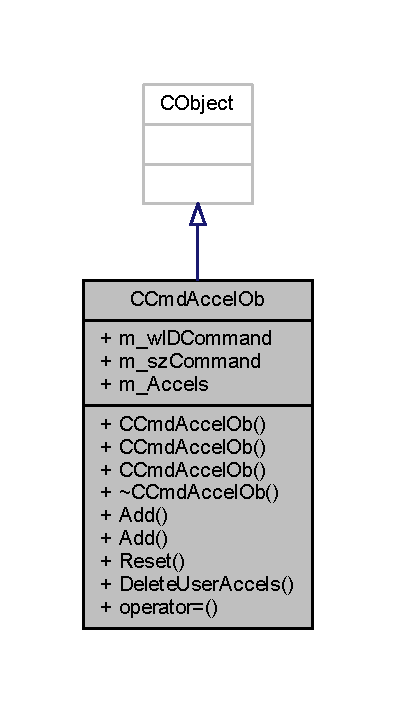
\includegraphics[width=190pt]{class_c_cmd_accel_ob__inherit__graph}
\end{center}
\end{figure}


C\+Cmd\+Accel\+Ob에 대한 협력 다이어그램\+:\nopagebreak
\begin{figure}[H]
\begin{center}
\leavevmode
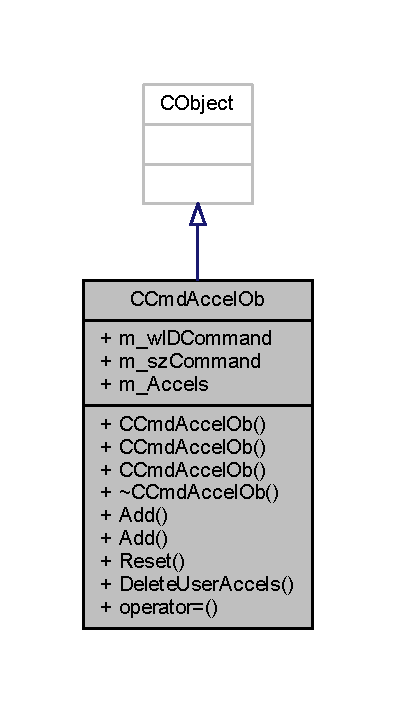
\includegraphics[width=190pt]{class_c_cmd_accel_ob__coll__graph}
\end{center}
\end{figure}
\subsection*{Public 멤버 함수}
\begin{DoxyCompactItemize}
\item 
\mbox{\hyperlink{class_c_cmd_accel_ob_a2f5bb136c7ba36c31551cec05f3c47fc}{C\+Cmd\+Accel\+Ob}} ()
\item 
\mbox{\hyperlink{class_c_cmd_accel_ob_a245369282fbad17c28924e0568fa5bcc}{C\+Cmd\+Accel\+Ob}} (W\+O\+RD w\+I\+D\+Command, L\+P\+C\+T\+S\+TR sz\+Command)
\item 
\mbox{\hyperlink{class_c_cmd_accel_ob_a2c532e999fa7dcb99d7d9b1027cebbef}{C\+Cmd\+Accel\+Ob}} (B\+Y\+TE c\+Virt, W\+O\+RD w\+I\+D\+Command, W\+O\+RD w\+Key, L\+P\+C\+T\+S\+TR sz\+Command, bool b\+Locked=false)
\item 
\mbox{\hyperlink{class_c_cmd_accel_ob_a41d00fee4f058c03fa85630612e1ab69}{$\sim$\+C\+Cmd\+Accel\+Ob}} ()
\item 
void \mbox{\hyperlink{class_c_cmd_accel_ob_a519f8c7ac935b0d06531589e5427b656}{Add}} (\mbox{\hyperlink{class_c_accels_ob}{C\+Accels\+Ob}} $\ast$p\+Accel)
\item 
void \mbox{\hyperlink{class_c_cmd_accel_ob_a15429015a20179a0e181347f35ad9c58}{Add}} (B\+Y\+TE c\+Virt, W\+O\+RD w\+Key, bool b\+Locked=false)
\item 
void \mbox{\hyperlink{class_c_cmd_accel_ob_ac679e57ed400b175109af50ea2ce919d}{Reset}} ()
\item 
void \mbox{\hyperlink{class_c_cmd_accel_ob_a7040471adc76f057a1d79c9fdfb84fe8}{Delete\+User\+Accels}} ()
\item 
\mbox{\hyperlink{class_c_cmd_accel_ob}{C\+Cmd\+Accel\+Ob}} \& \mbox{\hyperlink{class_c_cmd_accel_ob_a045ce00d2465fefed857066eef1406a7}{operator=}} (\mbox{\hyperlink{getopt1_8c_a2c212835823e3c54a8ab6d95c652660e}{const}} \mbox{\hyperlink{class_c_cmd_accel_ob}{C\+Cmd\+Accel\+Ob}} \&\mbox{\hyperlink{expr_8cpp_a765533dfc643627999c751f7e1514664}{from}})
\end{DoxyCompactItemize}
\subsection*{Public 속성}
\begin{DoxyCompactItemize}
\item 
W\+O\+RD \mbox{\hyperlink{class_c_cmd_accel_ob_aa3eb02dcd39ff14763fdefd8fabd7591}{m\+\_\+w\+I\+D\+Command}}
\item 
C\+String \mbox{\hyperlink{class_c_cmd_accel_ob_acbd02cc68d3909b1e39b687e76f45d91}{m\+\_\+sz\+Command}}
\item 
C\+List$<$ \mbox{\hyperlink{class_c_accels_ob}{C\+Accels\+Ob}} $\ast$, \mbox{\hyperlink{class_c_accels_ob}{C\+Accels\+Ob}} $\ast$\&$>$ \mbox{\hyperlink{class_c_cmd_accel_ob_a85772f1ea9204af42b8a39a0135dc0f8}{m\+\_\+\+Accels}}
\end{DoxyCompactItemize}


\subsection{상세한 설명}


Cmd\+Accel\+Ob.\+h 파일의 82 번째 라인에서 정의되었습니다.



\subsection{생성자 \& 소멸자 문서화}
\mbox{\Hypertarget{class_c_cmd_accel_ob_a2f5bb136c7ba36c31551cec05f3c47fc}\label{class_c_cmd_accel_ob_a2f5bb136c7ba36c31551cec05f3c47fc}} 
\index{C\+Cmd\+Accel\+Ob@{C\+Cmd\+Accel\+Ob}!C\+Cmd\+Accel\+Ob@{C\+Cmd\+Accel\+Ob}}
\index{C\+Cmd\+Accel\+Ob@{C\+Cmd\+Accel\+Ob}!C\+Cmd\+Accel\+Ob@{C\+Cmd\+Accel\+Ob}}
\subsubsection{\texorpdfstring{C\+Cmd\+Accel\+Ob()}{CCmdAccelOb()}\hspace{0.1cm}{\footnotesize\ttfamily [1/3]}}
{\footnotesize\ttfamily C\+Cmd\+Accel\+Ob\+::\+C\+Cmd\+Accel\+Ob (\begin{DoxyParamCaption}{ }\end{DoxyParamCaption})}



Cmd\+Accel\+Ob.\+cpp 파일의 368 번째 라인에서 정의되었습니다.


\begin{DoxyCode}
369 \{
370 \}
\end{DoxyCode}
\mbox{\Hypertarget{class_c_cmd_accel_ob_a245369282fbad17c28924e0568fa5bcc}\label{class_c_cmd_accel_ob_a245369282fbad17c28924e0568fa5bcc}} 
\index{C\+Cmd\+Accel\+Ob@{C\+Cmd\+Accel\+Ob}!C\+Cmd\+Accel\+Ob@{C\+Cmd\+Accel\+Ob}}
\index{C\+Cmd\+Accel\+Ob@{C\+Cmd\+Accel\+Ob}!C\+Cmd\+Accel\+Ob@{C\+Cmd\+Accel\+Ob}}
\subsubsection{\texorpdfstring{C\+Cmd\+Accel\+Ob()}{CCmdAccelOb()}\hspace{0.1cm}{\footnotesize\ttfamily [2/3]}}
{\footnotesize\ttfamily C\+Cmd\+Accel\+Ob\+::\+C\+Cmd\+Accel\+Ob (\begin{DoxyParamCaption}\item[{W\+O\+RD}]{w\+I\+D\+Command,  }\item[{L\+P\+C\+T\+S\+TR}]{sz\+Command }\end{DoxyParamCaption})}



Cmd\+Accel\+Ob.\+cpp 파일의 376 번째 라인에서 정의되었습니다.


\begin{DoxyCode}
377 \{
378   ASSERT(szCommand != \mbox{\hyperlink{getopt1_8c_a070d2ce7b6bb7e5c05602aa8c308d0c4}{NULL}});
379 
380   \mbox{\hyperlink{class_c_cmd_accel_ob_aa3eb02dcd39ff14763fdefd8fabd7591}{m\_wIDCommand}} = wIDCommand;
381   \mbox{\hyperlink{class_c_cmd_accel_ob_acbd02cc68d3909b1e39b687e76f45d91}{m\_szCommand}} = szCommand;
382 \}
\end{DoxyCode}
\mbox{\Hypertarget{class_c_cmd_accel_ob_a2c532e999fa7dcb99d7d9b1027cebbef}\label{class_c_cmd_accel_ob_a2c532e999fa7dcb99d7d9b1027cebbef}} 
\index{C\+Cmd\+Accel\+Ob@{C\+Cmd\+Accel\+Ob}!C\+Cmd\+Accel\+Ob@{C\+Cmd\+Accel\+Ob}}
\index{C\+Cmd\+Accel\+Ob@{C\+Cmd\+Accel\+Ob}!C\+Cmd\+Accel\+Ob@{C\+Cmd\+Accel\+Ob}}
\subsubsection{\texorpdfstring{C\+Cmd\+Accel\+Ob()}{CCmdAccelOb()}\hspace{0.1cm}{\footnotesize\ttfamily [3/3]}}
{\footnotesize\ttfamily C\+Cmd\+Accel\+Ob\+::\+C\+Cmd\+Accel\+Ob (\begin{DoxyParamCaption}\item[{B\+Y\+TE}]{c\+Virt,  }\item[{W\+O\+RD}]{w\+I\+D\+Command,  }\item[{W\+O\+RD}]{w\+Key,  }\item[{L\+P\+C\+T\+S\+TR}]{sz\+Command,  }\item[{bool}]{b\+Locked = {\ttfamily false} }\end{DoxyParamCaption})}



Cmd\+Accel\+Ob.\+cpp 파일의 388 번째 라인에서 정의되었습니다.


\begin{DoxyCode}
389 \{
390   ASSERT(szCommand != \mbox{\hyperlink{getopt1_8c_a070d2ce7b6bb7e5c05602aa8c308d0c4}{NULL}});
391   
392   \mbox{\hyperlink{class_c_cmd_accel_ob_aa3eb02dcd39ff14763fdefd8fabd7591}{m\_wIDCommand}} = wIDCommand;
393   \mbox{\hyperlink{class_c_cmd_accel_ob_acbd02cc68d3909b1e39b687e76f45d91}{m\_szCommand}} = szCommand;
394   
395   \mbox{\hyperlink{class_c_accels_ob}{CAccelsOb}}* pAccel = DEBUG\_NEW \mbox{\hyperlink{class_c_accels_ob}{CAccelsOb}}(cVirt, wKey, bLocked);
396   ASSERT(pAccel != \mbox{\hyperlink{getopt1_8c_a070d2ce7b6bb7e5c05602aa8c308d0c4}{NULL}});
397   \mbox{\hyperlink{class_c_cmd_accel_ob_a85772f1ea9204af42b8a39a0135dc0f8}{m\_Accels}}.AddTail(pAccel);
398 \}
\end{DoxyCode}
\mbox{\Hypertarget{class_c_cmd_accel_ob_a41d00fee4f058c03fa85630612e1ab69}\label{class_c_cmd_accel_ob_a41d00fee4f058c03fa85630612e1ab69}} 
\index{C\+Cmd\+Accel\+Ob@{C\+Cmd\+Accel\+Ob}!````~C\+Cmd\+Accel\+Ob@{$\sim$\+C\+Cmd\+Accel\+Ob}}
\index{````~C\+Cmd\+Accel\+Ob@{$\sim$\+C\+Cmd\+Accel\+Ob}!C\+Cmd\+Accel\+Ob@{C\+Cmd\+Accel\+Ob}}
\subsubsection{\texorpdfstring{$\sim$\+C\+Cmd\+Accel\+Ob()}{~CCmdAccelOb()}}
{\footnotesize\ttfamily C\+Cmd\+Accel\+Ob\+::$\sim$\+C\+Cmd\+Accel\+Ob (\begin{DoxyParamCaption}{ }\end{DoxyParamCaption})}



Cmd\+Accel\+Ob.\+cpp 파일의 404 번째 라인에서 정의되었습니다.


\begin{DoxyCode}
405 \{
406   POSITION pos = \mbox{\hyperlink{class_c_cmd_accel_ob_a85772f1ea9204af42b8a39a0135dc0f8}{m\_Accels}}.GetHeadPosition();
407   \textcolor{keywordflow}{while} (pos != \mbox{\hyperlink{getopt1_8c_a070d2ce7b6bb7e5c05602aa8c308d0c4}{NULL}})
408     \textcolor{keyword}{delete} \mbox{\hyperlink{class_c_cmd_accel_ob_a85772f1ea9204af42b8a39a0135dc0f8}{m\_Accels}}.GetNext(pos);
409   \mbox{\hyperlink{class_c_cmd_accel_ob_a85772f1ea9204af42b8a39a0135dc0f8}{m\_Accels}}.RemoveAll();
410 \}
\end{DoxyCode}


\subsection{멤버 함수 문서화}
\mbox{\Hypertarget{class_c_cmd_accel_ob_a519f8c7ac935b0d06531589e5427b656}\label{class_c_cmd_accel_ob_a519f8c7ac935b0d06531589e5427b656}} 
\index{C\+Cmd\+Accel\+Ob@{C\+Cmd\+Accel\+Ob}!Add@{Add}}
\index{Add@{Add}!C\+Cmd\+Accel\+Ob@{C\+Cmd\+Accel\+Ob}}
\subsubsection{\texorpdfstring{Add()}{Add()}\hspace{0.1cm}{\footnotesize\ttfamily [1/2]}}
{\footnotesize\ttfamily void C\+Cmd\+Accel\+Ob\+::\+Add (\begin{DoxyParamCaption}\item[{\mbox{\hyperlink{class_c_accels_ob}{C\+Accels\+Ob}} $\ast$}]{p\+Accel }\end{DoxyParamCaption})}



Cmd\+Accel\+Ob.\+cpp 파일의 429 번째 라인에서 정의되었습니다.


\begin{DoxyCode}
430 \{
431   ASSERT(pAccel != \mbox{\hyperlink{getopt1_8c_a070d2ce7b6bb7e5c05602aa8c308d0c4}{NULL}});
432   \mbox{\hyperlink{class_c_cmd_accel_ob_a85772f1ea9204af42b8a39a0135dc0f8}{m\_Accels}}.AddTail(pAccel);
433 \}
\end{DoxyCode}
이 함수를 호출하는 함수들에 대한 그래프입니다.\+:
\nopagebreak
\begin{figure}[H]
\begin{center}
\leavevmode
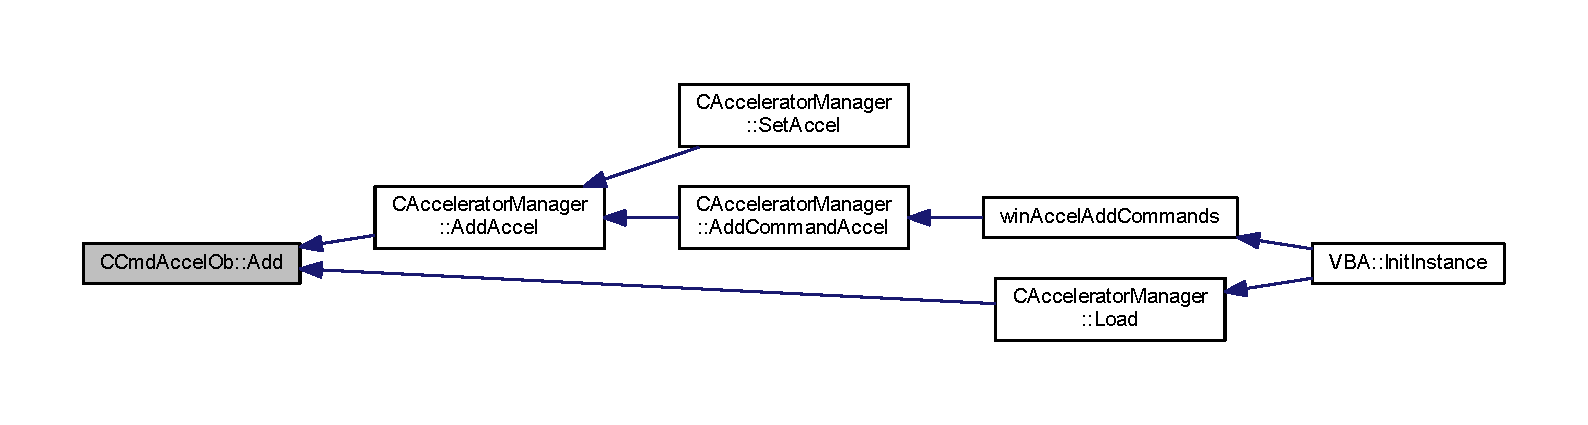
\includegraphics[width=350pt]{class_c_cmd_accel_ob_a519f8c7ac935b0d06531589e5427b656_icgraph}
\end{center}
\end{figure}
\mbox{\Hypertarget{class_c_cmd_accel_ob_a15429015a20179a0e181347f35ad9c58}\label{class_c_cmd_accel_ob_a15429015a20179a0e181347f35ad9c58}} 
\index{C\+Cmd\+Accel\+Ob@{C\+Cmd\+Accel\+Ob}!Add@{Add}}
\index{Add@{Add}!C\+Cmd\+Accel\+Ob@{C\+Cmd\+Accel\+Ob}}
\subsubsection{\texorpdfstring{Add()}{Add()}\hspace{0.1cm}{\footnotesize\ttfamily [2/2]}}
{\footnotesize\ttfamily void C\+Cmd\+Accel\+Ob\+::\+Add (\begin{DoxyParamCaption}\item[{B\+Y\+TE}]{c\+Virt,  }\item[{W\+O\+RD}]{w\+Key,  }\item[{bool}]{b\+Locked = {\ttfamily false} }\end{DoxyParamCaption})}



Cmd\+Accel\+Ob.\+cpp 파일의 418 번째 라인에서 정의되었습니다.


\begin{DoxyCode}
419 \{
420   \mbox{\hyperlink{class_c_accels_ob}{CAccelsOb}}* pAccel = DEBUG\_NEW \mbox{\hyperlink{class_c_accels_ob}{CAccelsOb}}(cVirt, wKey, bLocked);
421   ASSERT(pAccel != \mbox{\hyperlink{getopt1_8c_a070d2ce7b6bb7e5c05602aa8c308d0c4}{NULL}});
422   \mbox{\hyperlink{class_c_cmd_accel_ob_a85772f1ea9204af42b8a39a0135dc0f8}{m\_Accels}}.AddTail(pAccel);
423 \}
\end{DoxyCode}
\mbox{\Hypertarget{class_c_cmd_accel_ob_a7040471adc76f057a1d79c9fdfb84fe8}\label{class_c_cmd_accel_ob_a7040471adc76f057a1d79c9fdfb84fe8}} 
\index{C\+Cmd\+Accel\+Ob@{C\+Cmd\+Accel\+Ob}!Delete\+User\+Accels@{Delete\+User\+Accels}}
\index{Delete\+User\+Accels@{Delete\+User\+Accels}!C\+Cmd\+Accel\+Ob@{C\+Cmd\+Accel\+Ob}}
\subsubsection{\texorpdfstring{Delete\+User\+Accels()}{DeleteUserAccels()}}
{\footnotesize\ttfamily void C\+Cmd\+Accel\+Ob\+::\+Delete\+User\+Accels (\begin{DoxyParamCaption}{ }\end{DoxyParamCaption})}



Cmd\+Accel\+Ob.\+cpp 파일의 460 번째 라인에서 정의되었습니다.


\begin{DoxyCode}
461 \{
462   \mbox{\hyperlink{class_c_accels_ob}{CAccelsOb}}* pAccel;
463   POSITION prevPos;
464   POSITION pos = \mbox{\hyperlink{class_c_cmd_accel_ob_a85772f1ea9204af42b8a39a0135dc0f8}{m\_Accels}}.GetHeadPosition();
465   \textcolor{keywordflow}{while} (pos != \mbox{\hyperlink{getopt1_8c_a070d2ce7b6bb7e5c05602aa8c308d0c4}{NULL}}) \{
466     prevPos = pos;
467     pAccel = \mbox{\hyperlink{class_c_cmd_accel_ob_a85772f1ea9204af42b8a39a0135dc0f8}{m\_Accels}}.GetNext(pos);
468     \textcolor{keywordflow}{if} (!pAccel->\mbox{\hyperlink{class_c_accels_ob_ad8300bd20bd429ad61f89700e388dd9a}{m\_bLocked}}) \{
469       \textcolor{keyword}{delete} pAccel;
470       \mbox{\hyperlink{class_c_cmd_accel_ob_a85772f1ea9204af42b8a39a0135dc0f8}{m\_Accels}}.RemoveAt(prevPos);
471     \}
472   \}
473 \}
\end{DoxyCode}
이 함수를 호출하는 함수들에 대한 그래프입니다.\+:
\nopagebreak
\begin{figure}[H]
\begin{center}
\leavevmode
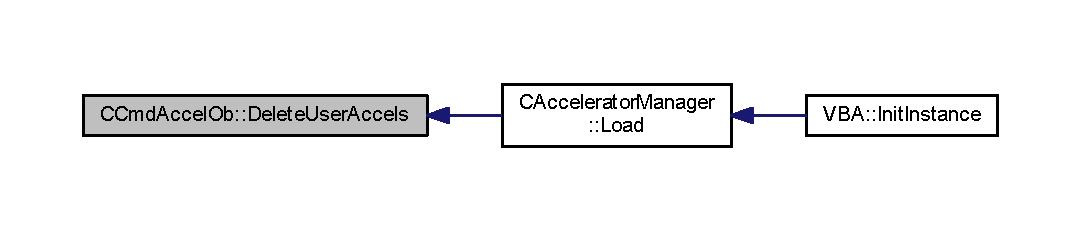
\includegraphics[width=350pt]{class_c_cmd_accel_ob_a7040471adc76f057a1d79c9fdfb84fe8_icgraph}
\end{center}
\end{figure}
\mbox{\Hypertarget{class_c_cmd_accel_ob_a045ce00d2465fefed857066eef1406a7}\label{class_c_cmd_accel_ob_a045ce00d2465fefed857066eef1406a7}} 
\index{C\+Cmd\+Accel\+Ob@{C\+Cmd\+Accel\+Ob}!operator=@{operator=}}
\index{operator=@{operator=}!C\+Cmd\+Accel\+Ob@{C\+Cmd\+Accel\+Ob}}
\subsubsection{\texorpdfstring{operator=()}{operator=()}}
{\footnotesize\ttfamily \mbox{\hyperlink{class_c_cmd_accel_ob}{C\+Cmd\+Accel\+Ob}} \& C\+Cmd\+Accel\+Ob\+::operator= (\begin{DoxyParamCaption}\item[{\mbox{\hyperlink{getopt1_8c_a2c212835823e3c54a8ab6d95c652660e}{const}} \mbox{\hyperlink{class_c_cmd_accel_ob}{C\+Cmd\+Accel\+Ob}} \&}]{from }\end{DoxyParamCaption})}



Cmd\+Accel\+Ob.\+cpp 파일의 439 번째 라인에서 정의되었습니다.


\begin{DoxyCode}
440 \{
441   \mbox{\hyperlink{class_c_cmd_accel_ob_ac679e57ed400b175109af50ea2ce919d}{Reset}}();
442   
443   \mbox{\hyperlink{class_c_cmd_accel_ob_aa3eb02dcd39ff14763fdefd8fabd7591}{m\_wIDCommand}} = \mbox{\hyperlink{expr_8cpp_a765533dfc643627999c751f7e1514664}{from}}.m\_wIDCommand;
444   \mbox{\hyperlink{class_c_cmd_accel_ob_acbd02cc68d3909b1e39b687e76f45d91}{m\_szCommand}} = \mbox{\hyperlink{expr_8cpp_a765533dfc643627999c751f7e1514664}{from}}.m\_szCommand;
445   
446   \mbox{\hyperlink{class_c_accels_ob}{CAccelsOb}}* pAccel;
447   POSITION pos = \mbox{\hyperlink{expr_8cpp_a765533dfc643627999c751f7e1514664}{from}}.m\_Accels.GetHeadPosition();
448   \textcolor{keywordflow}{while} (pos != \mbox{\hyperlink{getopt1_8c_a070d2ce7b6bb7e5c05602aa8c308d0c4}{NULL}}) \{
449     pAccel = DEBUG\_NEW \mbox{\hyperlink{class_c_accels_ob}{CAccelsOb}}(\mbox{\hyperlink{expr_8cpp_a765533dfc643627999c751f7e1514664}{from}}.m\_Accels.GetNext(pos));
450     ASSERT(pAccel != \mbox{\hyperlink{getopt1_8c_a070d2ce7b6bb7e5c05602aa8c308d0c4}{NULL}});
451     \mbox{\hyperlink{class_c_cmd_accel_ob_a85772f1ea9204af42b8a39a0135dc0f8}{m\_Accels}}.AddTail(pAccel);
452   \}
453   \textcolor{keywordflow}{return} *\textcolor{keyword}{this};
454 \}
\end{DoxyCode}
이 함수 내부에서 호출하는 함수들에 대한 그래프입니다.\+:
\nopagebreak
\begin{figure}[H]
\begin{center}
\leavevmode
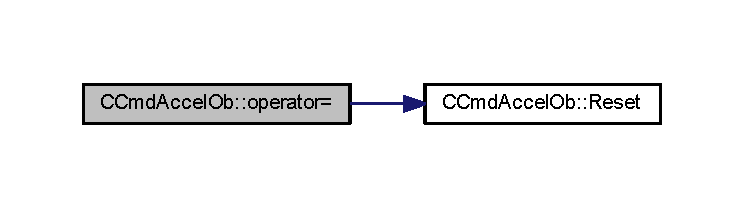
\includegraphics[width=350pt]{class_c_cmd_accel_ob_a045ce00d2465fefed857066eef1406a7_cgraph}
\end{center}
\end{figure}
\mbox{\Hypertarget{class_c_cmd_accel_ob_ac679e57ed400b175109af50ea2ce919d}\label{class_c_cmd_accel_ob_ac679e57ed400b175109af50ea2ce919d}} 
\index{C\+Cmd\+Accel\+Ob@{C\+Cmd\+Accel\+Ob}!Reset@{Reset}}
\index{Reset@{Reset}!C\+Cmd\+Accel\+Ob@{C\+Cmd\+Accel\+Ob}}
\subsubsection{\texorpdfstring{Reset()}{Reset()}}
{\footnotesize\ttfamily void C\+Cmd\+Accel\+Ob\+::\+Reset (\begin{DoxyParamCaption}{ }\end{DoxyParamCaption})}



Cmd\+Accel\+Ob.\+cpp 파일의 479 번째 라인에서 정의되었습니다.


\begin{DoxyCode}
480 \{
481   \mbox{\hyperlink{class_c_cmd_accel_ob_aa3eb02dcd39ff14763fdefd8fabd7591}{m\_wIDCommand}} = 0;
482   \mbox{\hyperlink{class_c_cmd_accel_ob_acbd02cc68d3909b1e39b687e76f45d91}{m\_szCommand}} = \textcolor{stringliteral}{"Empty command"};
483   
484   \mbox{\hyperlink{class_c_accels_ob}{CAccelsOb}}* pAccel;
485   POSITION pos = \mbox{\hyperlink{class_c_cmd_accel_ob_a85772f1ea9204af42b8a39a0135dc0f8}{m\_Accels}}.GetHeadPosition();
486   \textcolor{keywordflow}{while} (pos != \mbox{\hyperlink{getopt1_8c_a070d2ce7b6bb7e5c05602aa8c308d0c4}{NULL}}) \{
487     pAccel = \mbox{\hyperlink{class_c_cmd_accel_ob_a85772f1ea9204af42b8a39a0135dc0f8}{m\_Accels}}.GetNext(pos);
488     \textcolor{keyword}{delete} pAccel;
489   \}
490 \}
\end{DoxyCode}
이 함수를 호출하는 함수들에 대한 그래프입니다.\+:
\nopagebreak
\begin{figure}[H]
\begin{center}
\leavevmode
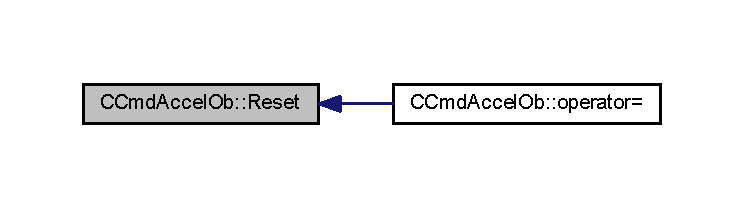
\includegraphics[width=350pt]{class_c_cmd_accel_ob_ac679e57ed400b175109af50ea2ce919d_icgraph}
\end{center}
\end{figure}


\subsection{멤버 데이터 문서화}
\mbox{\Hypertarget{class_c_cmd_accel_ob_a85772f1ea9204af42b8a39a0135dc0f8}\label{class_c_cmd_accel_ob_a85772f1ea9204af42b8a39a0135dc0f8}} 
\index{C\+Cmd\+Accel\+Ob@{C\+Cmd\+Accel\+Ob}!m\+\_\+\+Accels@{m\+\_\+\+Accels}}
\index{m\+\_\+\+Accels@{m\+\_\+\+Accels}!C\+Cmd\+Accel\+Ob@{C\+Cmd\+Accel\+Ob}}
\subsubsection{\texorpdfstring{m\+\_\+\+Accels}{m\_Accels}}
{\footnotesize\ttfamily C\+List$<$ \mbox{\hyperlink{class_c_accels_ob}{C\+Accels\+Ob}}$\ast$, \mbox{\hyperlink{class_c_accels_ob}{C\+Accels\+Ob}}$\ast$\& $>$ C\+Cmd\+Accel\+Ob\+::m\+\_\+\+Accels}



Cmd\+Accel\+Ob.\+h 파일의 106 번째 라인에서 정의되었습니다.

\mbox{\Hypertarget{class_c_cmd_accel_ob_acbd02cc68d3909b1e39b687e76f45d91}\label{class_c_cmd_accel_ob_acbd02cc68d3909b1e39b687e76f45d91}} 
\index{C\+Cmd\+Accel\+Ob@{C\+Cmd\+Accel\+Ob}!m\+\_\+sz\+Command@{m\+\_\+sz\+Command}}
\index{m\+\_\+sz\+Command@{m\+\_\+sz\+Command}!C\+Cmd\+Accel\+Ob@{C\+Cmd\+Accel\+Ob}}
\subsubsection{\texorpdfstring{m\+\_\+sz\+Command}{m\_szCommand}}
{\footnotesize\ttfamily C\+String C\+Cmd\+Accel\+Ob\+::m\+\_\+sz\+Command}



Cmd\+Accel\+Ob.\+h 파일의 104 번째 라인에서 정의되었습니다.

\mbox{\Hypertarget{class_c_cmd_accel_ob_aa3eb02dcd39ff14763fdefd8fabd7591}\label{class_c_cmd_accel_ob_aa3eb02dcd39ff14763fdefd8fabd7591}} 
\index{C\+Cmd\+Accel\+Ob@{C\+Cmd\+Accel\+Ob}!m\+\_\+w\+I\+D\+Command@{m\+\_\+w\+I\+D\+Command}}
\index{m\+\_\+w\+I\+D\+Command@{m\+\_\+w\+I\+D\+Command}!C\+Cmd\+Accel\+Ob@{C\+Cmd\+Accel\+Ob}}
\subsubsection{\texorpdfstring{m\+\_\+w\+I\+D\+Command}{m\_wIDCommand}}
{\footnotesize\ttfamily W\+O\+RD C\+Cmd\+Accel\+Ob\+::m\+\_\+w\+I\+D\+Command}



Cmd\+Accel\+Ob.\+h 파일의 103 번째 라인에서 정의되었습니다.



이 클래스에 대한 문서화 페이지는 다음의 파일들로부터 생성되었습니다.\+:\begin{DoxyCompactItemize}
\item 
C\+:/\+Users/sjh13/sources/\+Visual\+Boy\+Advance/src/win32/\mbox{\hyperlink{_cmd_accel_ob_8h}{Cmd\+Accel\+Ob.\+h}}\item 
C\+:/\+Users/sjh13/sources/\+Visual\+Boy\+Advance/src/win32/\mbox{\hyperlink{_cmd_accel_ob_8cpp}{Cmd\+Accel\+Ob.\+cpp}}\end{DoxyCompactItemize}

\hypertarget{class_win_helper_1_1_c_critical_section}{}\section{Win\+Helper\+:\+:C\+Critical\+Section 클래스 참조}
\label{class_win_helper_1_1_c_critical_section}\index{Win\+Helper\+::\+C\+Critical\+Section@{Win\+Helper\+::\+C\+Critical\+Section}}
\subsection*{클래스}
\begin{DoxyCompactItemize}
\item 
class \mbox{\hyperlink{class_win_helper_1_1_c_critical_section_1_1_c_lock}{C\+Lock}}
\end{DoxyCompactItemize}
\subsection*{Public 멤버 함수}
\begin{DoxyCompactItemize}
\item 
\mbox{\Hypertarget{class_win_helper_1_1_c_critical_section_aa0c20ee0e7de698b37c26a295d0f45fe}\label{class_win_helper_1_1_c_critical_section_aa0c20ee0e7de698b37c26a295d0f45fe}} 
void {\bfseries Lock} ()
\item 
\mbox{\Hypertarget{class_win_helper_1_1_c_critical_section_a32b6fc61701020c400f3bb9b5e00bf12}\label{class_win_helper_1_1_c_critical_section_a32b6fc61701020c400f3bb9b5e00bf12}} 
void {\bfseries Unlock} ()
\end{DoxyCompactItemize}


이 클래스에 대한 문서화 페이지는 다음의 파일로부터 생성되었습니다.\+:\begin{DoxyCompactItemize}
\item 
src/win32/Win\+Helper.\+h\end{DoxyCompactItemize}

\hypertarget{class_win_helper_1_1_c_defer_window_pos}{}\section{Win\+Helper\+:\+:C\+Defer\+Window\+Pos 클래스 참조}
\label{class_win_helper_1_1_c_defer_window_pos}\index{Win\+Helper\+::\+C\+Defer\+Window\+Pos@{Win\+Helper\+::\+C\+Defer\+Window\+Pos}}
\subsection*{Public 멤버 함수}
\begin{DoxyCompactItemize}
\item 
\mbox{\Hypertarget{class_win_helper_1_1_c_defer_window_pos_ac98b161abd5044c2a2e1e8b8efa0744f}\label{class_win_helper_1_1_c_defer_window_pos_ac98b161abd5044c2a2e1e8b8efa0744f}} 
{\bfseries C\+Defer\+Window\+Pos} (const int n\+Windows=1)
\item 
\mbox{\Hypertarget{class_win_helper_1_1_c_defer_window_pos_a50e9a5dfc382996381a506d66f94efd6}\label{class_win_helper_1_1_c_defer_window_pos_a50e9a5dfc382996381a506d66f94efd6}} 
H\+D\+WP {\bfseries Defer\+Window\+Pos} (H\+W\+ND h\+Wnd, H\+W\+ND h\+Wnd\+Insert\+After, int x, int y, int cx, int cy, U\+I\+NT u\+Flags)
\item 
\mbox{\Hypertarget{class_win_helper_1_1_c_defer_window_pos_aeba6047e5182577c14bfe4729a602ca9}\label{class_win_helper_1_1_c_defer_window_pos_aeba6047e5182577c14bfe4729a602ca9}} 
H\+D\+WP {\bfseries Defer\+Window\+Pos} (H\+W\+ND h\+Wnd, H\+W\+ND h\+Wnd\+Insert\+After, const \mbox{\hyperlink{class_win_helper_1_1_c_rect}{C\+Rect}} \&rc, U\+I\+NT u\+Flags)
\end{DoxyCompactItemize}


이 클래스에 대한 문서화 페이지는 다음의 파일로부터 생성되었습니다.\+:\begin{DoxyCompactItemize}
\item 
src/win32/Win\+Helper.\+h\end{DoxyCompactItemize}

\hypertarget{struct_cheats_data}{}\section{Cheats\+Data 구조체 참조}
\label{struct_cheats_data}\index{Cheats\+Data@{Cheats\+Data}}


{\ttfamily \#include $<$Cheats.\+h$>$}



Cheats\+Data에 대한 협력 다이어그램\+:\nopagebreak
\begin{figure}[H]
\begin{center}
\leavevmode
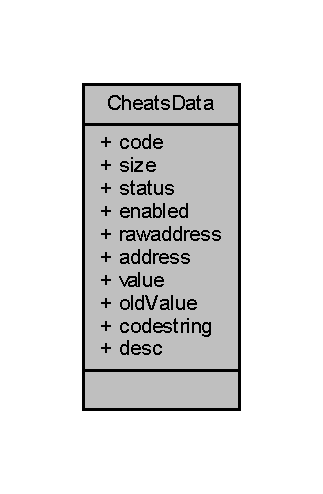
\includegraphics[width=155pt]{struct_cheats_data__coll__graph}
\end{center}
\end{figure}
\subsection*{Public 속성}
\begin{DoxyCompactItemize}
\item 
\mbox{\hyperlink{_util_8cpp_a0ef32aa8672df19503a49fab2d0c8071}{int}} \mbox{\hyperlink{struct_cheats_data_a24cc3911cdbf485ce42b401873e2e269}{code}}
\item 
\mbox{\hyperlink{_util_8cpp_a0ef32aa8672df19503a49fab2d0c8071}{int}} \mbox{\hyperlink{struct_cheats_data_a2e3e50db1415e980fe34da90fdbda02a}{size}}
\item 
\mbox{\hyperlink{_util_8cpp_a0ef32aa8672df19503a49fab2d0c8071}{int}} \mbox{\hyperlink{struct_cheats_data_aeb36cfefe89db53cdb45909d35b9c6e4}{status}}
\item 
bool \mbox{\hyperlink{struct_cheats_data_a99c72fc2074645888a5afe88cfb0fd15}{enabled}}
\item 
\mbox{\hyperlink{_system_8h_a10e94b422ef0c20dcdec20d31a1f5049}{u32}} \mbox{\hyperlink{struct_cheats_data_aa12c1d606385a21c544022d5acb9c95e}{rawaddress}}
\item 
\mbox{\hyperlink{_system_8h_a10e94b422ef0c20dcdec20d31a1f5049}{u32}} \mbox{\hyperlink{struct_cheats_data_a01fd4bf820cf8cb6a4212183b29530cd}{address}}
\item 
\mbox{\hyperlink{_system_8h_a10e94b422ef0c20dcdec20d31a1f5049}{u32}} \mbox{\hyperlink{struct_cheats_data_ab0df909850861e6314b1abb13c6305d1}{value}}
\item 
\mbox{\hyperlink{_system_8h_a10e94b422ef0c20dcdec20d31a1f5049}{u32}} \mbox{\hyperlink{struct_cheats_data_ae53ec4ba23eb94b339cc05b807a944d5}{old\+Value}}
\item 
char \mbox{\hyperlink{struct_cheats_data_a4163c46e82595675cedca34ad19d6f43}{codestring}} \mbox{[}20\mbox{]}
\item 
char \mbox{\hyperlink{struct_cheats_data_a12223e792c360411d694a8e2506dc90e}{desc}} \mbox{[}32\mbox{]}
\end{DoxyCompactItemize}


\subsection{상세한 설명}


Cheats.\+h 파일의 23 번째 라인에서 정의되었습니다.



\subsection{멤버 데이터 문서화}
\mbox{\Hypertarget{struct_cheats_data_a01fd4bf820cf8cb6a4212183b29530cd}\label{struct_cheats_data_a01fd4bf820cf8cb6a4212183b29530cd}} 
\index{Cheats\+Data@{Cheats\+Data}!address@{address}}
\index{address@{address}!Cheats\+Data@{Cheats\+Data}}
\subsubsection{\texorpdfstring{address}{address}}
{\footnotesize\ttfamily \mbox{\hyperlink{_system_8h_a10e94b422ef0c20dcdec20d31a1f5049}{u32}} Cheats\+Data\+::address}



Cheats.\+h 파일의 29 번째 라인에서 정의되었습니다.

\mbox{\Hypertarget{struct_cheats_data_a24cc3911cdbf485ce42b401873e2e269}\label{struct_cheats_data_a24cc3911cdbf485ce42b401873e2e269}} 
\index{Cheats\+Data@{Cheats\+Data}!code@{code}}
\index{code@{code}!Cheats\+Data@{Cheats\+Data}}
\subsubsection{\texorpdfstring{code}{code}}
{\footnotesize\ttfamily \mbox{\hyperlink{_util_8cpp_a0ef32aa8672df19503a49fab2d0c8071}{int}} Cheats\+Data\+::code}



Cheats.\+h 파일의 24 번째 라인에서 정의되었습니다.

\mbox{\Hypertarget{struct_cheats_data_a4163c46e82595675cedca34ad19d6f43}\label{struct_cheats_data_a4163c46e82595675cedca34ad19d6f43}} 
\index{Cheats\+Data@{Cheats\+Data}!codestring@{codestring}}
\index{codestring@{codestring}!Cheats\+Data@{Cheats\+Data}}
\subsubsection{\texorpdfstring{codestring}{codestring}}
{\footnotesize\ttfamily char Cheats\+Data\+::codestring\mbox{[}20\mbox{]}}



Cheats.\+h 파일의 32 번째 라인에서 정의되었습니다.

\mbox{\Hypertarget{struct_cheats_data_a12223e792c360411d694a8e2506dc90e}\label{struct_cheats_data_a12223e792c360411d694a8e2506dc90e}} 
\index{Cheats\+Data@{Cheats\+Data}!desc@{desc}}
\index{desc@{desc}!Cheats\+Data@{Cheats\+Data}}
\subsubsection{\texorpdfstring{desc}{desc}}
{\footnotesize\ttfamily char Cheats\+Data\+::desc\mbox{[}32\mbox{]}}



Cheats.\+h 파일의 33 번째 라인에서 정의되었습니다.

\mbox{\Hypertarget{struct_cheats_data_a99c72fc2074645888a5afe88cfb0fd15}\label{struct_cheats_data_a99c72fc2074645888a5afe88cfb0fd15}} 
\index{Cheats\+Data@{Cheats\+Data}!enabled@{enabled}}
\index{enabled@{enabled}!Cheats\+Data@{Cheats\+Data}}
\subsubsection{\texorpdfstring{enabled}{enabled}}
{\footnotesize\ttfamily bool Cheats\+Data\+::enabled}



Cheats.\+h 파일의 27 번째 라인에서 정의되었습니다.

\mbox{\Hypertarget{struct_cheats_data_ae53ec4ba23eb94b339cc05b807a944d5}\label{struct_cheats_data_ae53ec4ba23eb94b339cc05b807a944d5}} 
\index{Cheats\+Data@{Cheats\+Data}!old\+Value@{old\+Value}}
\index{old\+Value@{old\+Value}!Cheats\+Data@{Cheats\+Data}}
\subsubsection{\texorpdfstring{old\+Value}{oldValue}}
{\footnotesize\ttfamily \mbox{\hyperlink{_system_8h_a10e94b422ef0c20dcdec20d31a1f5049}{u32}} Cheats\+Data\+::old\+Value}



Cheats.\+h 파일의 31 번째 라인에서 정의되었습니다.

\mbox{\Hypertarget{struct_cheats_data_aa12c1d606385a21c544022d5acb9c95e}\label{struct_cheats_data_aa12c1d606385a21c544022d5acb9c95e}} 
\index{Cheats\+Data@{Cheats\+Data}!rawaddress@{rawaddress}}
\index{rawaddress@{rawaddress}!Cheats\+Data@{Cheats\+Data}}
\subsubsection{\texorpdfstring{rawaddress}{rawaddress}}
{\footnotesize\ttfamily \mbox{\hyperlink{_system_8h_a10e94b422ef0c20dcdec20d31a1f5049}{u32}} Cheats\+Data\+::rawaddress}



Cheats.\+h 파일의 28 번째 라인에서 정의되었습니다.

\mbox{\Hypertarget{struct_cheats_data_a2e3e50db1415e980fe34da90fdbda02a}\label{struct_cheats_data_a2e3e50db1415e980fe34da90fdbda02a}} 
\index{Cheats\+Data@{Cheats\+Data}!size@{size}}
\index{size@{size}!Cheats\+Data@{Cheats\+Data}}
\subsubsection{\texorpdfstring{size}{size}}
{\footnotesize\ttfamily \mbox{\hyperlink{_util_8cpp_a0ef32aa8672df19503a49fab2d0c8071}{int}} Cheats\+Data\+::size}



Cheats.\+h 파일의 25 번째 라인에서 정의되었습니다.

\mbox{\Hypertarget{struct_cheats_data_aeb36cfefe89db53cdb45909d35b9c6e4}\label{struct_cheats_data_aeb36cfefe89db53cdb45909d35b9c6e4}} 
\index{Cheats\+Data@{Cheats\+Data}!status@{status}}
\index{status@{status}!Cheats\+Data@{Cheats\+Data}}
\subsubsection{\texorpdfstring{status}{status}}
{\footnotesize\ttfamily \mbox{\hyperlink{_util_8cpp_a0ef32aa8672df19503a49fab2d0c8071}{int}} Cheats\+Data\+::status}



Cheats.\+h 파일의 26 번째 라인에서 정의되었습니다.

\mbox{\Hypertarget{struct_cheats_data_ab0df909850861e6314b1abb13c6305d1}\label{struct_cheats_data_ab0df909850861e6314b1abb13c6305d1}} 
\index{Cheats\+Data@{Cheats\+Data}!value@{value}}
\index{value@{value}!Cheats\+Data@{Cheats\+Data}}
\subsubsection{\texorpdfstring{value}{value}}
{\footnotesize\ttfamily \mbox{\hyperlink{_system_8h_a10e94b422ef0c20dcdec20d31a1f5049}{u32}} Cheats\+Data\+::value}



Cheats.\+h 파일의 30 번째 라인에서 정의되었습니다.



이 구조체에 대한 문서화 페이지는 다음의 파일로부터 생성되었습니다.\+:\begin{DoxyCompactItemize}
\item 
C\+:/\+Users/sjh13/sources/\+Visual\+Boy\+Advance/src/\mbox{\hyperlink{_cheats_8h}{Cheats.\+h}}\end{DoxyCompactItemize}

\hypertarget{struct_cheat_search_block}{}\section{Cheat\+Search\+Block 구조체 참조}
\label{struct_cheat_search_block}\index{Cheat\+Search\+Block@{Cheat\+Search\+Block}}


{\ttfamily \#include $<$Cheat\+Search.\+h$>$}



Cheat\+Search\+Block에 대한 협력 다이어그램\+:\nopagebreak
\begin{figure}[H]
\begin{center}
\leavevmode
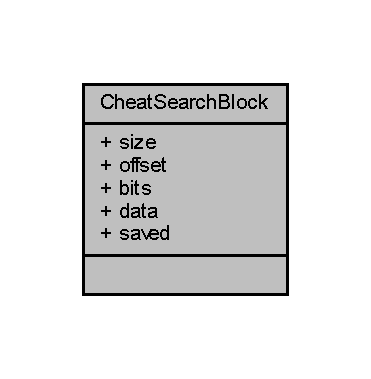
\includegraphics[width=178pt]{struct_cheat_search_block__coll__graph}
\end{center}
\end{figure}
\subsection*{Public 속성}
\begin{DoxyCompactItemize}
\item 
\mbox{\hyperlink{_util_8cpp_a0ef32aa8672df19503a49fab2d0c8071}{int}} \mbox{\hyperlink{struct_cheat_search_block_aaaf9517229363e8807cd511022d90012}{size}}
\item 
\mbox{\hyperlink{_system_8h_a10e94b422ef0c20dcdec20d31a1f5049}{u32}} \mbox{\hyperlink{struct_cheat_search_block_a33001049203a8b1b625ccdd29bf57d8f}{offset}}
\item 
\mbox{\hyperlink{_system_8h_aed742c436da53c1080638ce6ef7d13de}{u8}} $\ast$ \mbox{\hyperlink{struct_cheat_search_block_a59258efebf4223be206ad11d3ca8ebf4}{bits}}
\item 
\mbox{\hyperlink{_system_8h_aed742c436da53c1080638ce6ef7d13de}{u8}} $\ast$ \mbox{\hyperlink{struct_cheat_search_block_aa3a8235324df132c5fc67c5239748f15}{data}}
\item 
\mbox{\hyperlink{_system_8h_aed742c436da53c1080638ce6ef7d13de}{u8}} $\ast$ \mbox{\hyperlink{struct_cheat_search_block_af2b921cffd3f8d9420a8b9a3a33752ca}{saved}}
\end{DoxyCompactItemize}


\subsection{상세한 설명}


Cheat\+Search.\+h 파일의 25 번째 라인에서 정의되었습니다.



\subsection{멤버 데이터 문서화}
\mbox{\Hypertarget{struct_cheat_search_block_a59258efebf4223be206ad11d3ca8ebf4}\label{struct_cheat_search_block_a59258efebf4223be206ad11d3ca8ebf4}} 
\index{Cheat\+Search\+Block@{Cheat\+Search\+Block}!bits@{bits}}
\index{bits@{bits}!Cheat\+Search\+Block@{Cheat\+Search\+Block}}
\subsubsection{\texorpdfstring{bits}{bits}}
{\footnotesize\ttfamily \mbox{\hyperlink{_system_8h_aed742c436da53c1080638ce6ef7d13de}{u8}}$\ast$ Cheat\+Search\+Block\+::bits}



Cheat\+Search.\+h 파일의 28 번째 라인에서 정의되었습니다.

\mbox{\Hypertarget{struct_cheat_search_block_aa3a8235324df132c5fc67c5239748f15}\label{struct_cheat_search_block_aa3a8235324df132c5fc67c5239748f15}} 
\index{Cheat\+Search\+Block@{Cheat\+Search\+Block}!data@{data}}
\index{data@{data}!Cheat\+Search\+Block@{Cheat\+Search\+Block}}
\subsubsection{\texorpdfstring{data}{data}}
{\footnotesize\ttfamily \mbox{\hyperlink{_system_8h_aed742c436da53c1080638ce6ef7d13de}{u8}}$\ast$ Cheat\+Search\+Block\+::data}



Cheat\+Search.\+h 파일의 29 번째 라인에서 정의되었습니다.

\mbox{\Hypertarget{struct_cheat_search_block_a33001049203a8b1b625ccdd29bf57d8f}\label{struct_cheat_search_block_a33001049203a8b1b625ccdd29bf57d8f}} 
\index{Cheat\+Search\+Block@{Cheat\+Search\+Block}!offset@{offset}}
\index{offset@{offset}!Cheat\+Search\+Block@{Cheat\+Search\+Block}}
\subsubsection{\texorpdfstring{offset}{offset}}
{\footnotesize\ttfamily \mbox{\hyperlink{_system_8h_a10e94b422ef0c20dcdec20d31a1f5049}{u32}} Cheat\+Search\+Block\+::offset}



Cheat\+Search.\+h 파일의 27 번째 라인에서 정의되었습니다.

\mbox{\Hypertarget{struct_cheat_search_block_af2b921cffd3f8d9420a8b9a3a33752ca}\label{struct_cheat_search_block_af2b921cffd3f8d9420a8b9a3a33752ca}} 
\index{Cheat\+Search\+Block@{Cheat\+Search\+Block}!saved@{saved}}
\index{saved@{saved}!Cheat\+Search\+Block@{Cheat\+Search\+Block}}
\subsubsection{\texorpdfstring{saved}{saved}}
{\footnotesize\ttfamily \mbox{\hyperlink{_system_8h_aed742c436da53c1080638ce6ef7d13de}{u8}}$\ast$ Cheat\+Search\+Block\+::saved}



Cheat\+Search.\+h 파일의 30 번째 라인에서 정의되었습니다.

\mbox{\Hypertarget{struct_cheat_search_block_aaaf9517229363e8807cd511022d90012}\label{struct_cheat_search_block_aaaf9517229363e8807cd511022d90012}} 
\index{Cheat\+Search\+Block@{Cheat\+Search\+Block}!size@{size}}
\index{size@{size}!Cheat\+Search\+Block@{Cheat\+Search\+Block}}
\subsubsection{\texorpdfstring{size}{size}}
{\footnotesize\ttfamily \mbox{\hyperlink{_util_8cpp_a0ef32aa8672df19503a49fab2d0c8071}{int}} Cheat\+Search\+Block\+::size}



Cheat\+Search.\+h 파일의 26 번째 라인에서 정의되었습니다.



이 구조체에 대한 문서화 페이지는 다음의 파일로부터 생성되었습니다.\+:\begin{DoxyCompactItemize}
\item 
C\+:/\+Users/sjh13/sources/\+Visual\+Boy\+Advance/src/\mbox{\hyperlink{_cheat_search_8h}{Cheat\+Search.\+h}}\end{DoxyCompactItemize}

\hypertarget{struct_cheat_search_data}{}\section{Cheat\+Search\+Data 구조체 참조}
\label{struct_cheat_search_data}\index{Cheat\+Search\+Data@{Cheat\+Search\+Data}}


{\ttfamily \#include $<$Cheat\+Search.\+h$>$}



Cheat\+Search\+Data에 대한 협력 다이어그램\+:\nopagebreak
\begin{figure}[H]
\begin{center}
\leavevmode
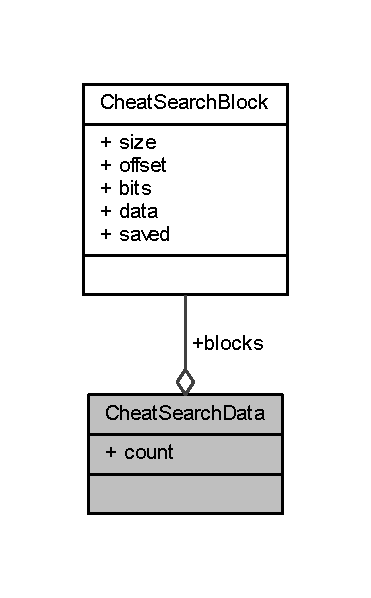
\includegraphics[width=178pt]{struct_cheat_search_data__coll__graph}
\end{center}
\end{figure}
\subsection*{Public 속성}
\begin{DoxyCompactItemize}
\item 
\mbox{\hyperlink{_util_8cpp_a0ef32aa8672df19503a49fab2d0c8071}{int}} \mbox{\hyperlink{struct_cheat_search_data_a4c4d3092ddaff068d820c28067b15774}{count}}
\item 
\mbox{\hyperlink{struct_cheat_search_block}{Cheat\+Search\+Block}} $\ast$ \mbox{\hyperlink{struct_cheat_search_data_ae0235bdc2000cc25b8c072442ce33c2c}{blocks}}
\end{DoxyCompactItemize}


\subsection{상세한 설명}


Cheat\+Search.\+h 파일의 33 번째 라인에서 정의되었습니다.



\subsection{멤버 데이터 문서화}
\mbox{\Hypertarget{struct_cheat_search_data_ae0235bdc2000cc25b8c072442ce33c2c}\label{struct_cheat_search_data_ae0235bdc2000cc25b8c072442ce33c2c}} 
\index{Cheat\+Search\+Data@{Cheat\+Search\+Data}!blocks@{blocks}}
\index{blocks@{blocks}!Cheat\+Search\+Data@{Cheat\+Search\+Data}}
\subsubsection{\texorpdfstring{blocks}{blocks}}
{\footnotesize\ttfamily \mbox{\hyperlink{struct_cheat_search_block}{Cheat\+Search\+Block}}$\ast$ Cheat\+Search\+Data\+::blocks}



Cheat\+Search.\+h 파일의 35 번째 라인에서 정의되었습니다.

\mbox{\Hypertarget{struct_cheat_search_data_a4c4d3092ddaff068d820c28067b15774}\label{struct_cheat_search_data_a4c4d3092ddaff068d820c28067b15774}} 
\index{Cheat\+Search\+Data@{Cheat\+Search\+Data}!count@{count}}
\index{count@{count}!Cheat\+Search\+Data@{Cheat\+Search\+Data}}
\subsubsection{\texorpdfstring{count}{count}}
{\footnotesize\ttfamily \mbox{\hyperlink{_util_8cpp_a0ef32aa8672df19503a49fab2d0c8071}{int}} Cheat\+Search\+Data\+::count}



Cheat\+Search.\+h 파일의 34 번째 라인에서 정의되었습니다.



이 구조체에 대한 문서화 페이지는 다음의 파일로부터 생성되었습니다.\+:\begin{DoxyCompactItemize}
\item 
C\+:/\+Users/sjh13/sources/\+Visual\+Boy\+Advance/src/\mbox{\hyperlink{_cheat_search_8h}{Cheat\+Search.\+h}}\end{DoxyCompactItemize}

\hypertarget{class_c_keyboard_edit}{}\section{C\+Keyboard\+Edit 클래스 참조}
\label{class_c_keyboard_edit}\index{C\+Keyboard\+Edit@{C\+Keyboard\+Edit}}


{\ttfamily \#include $<$Keyboard\+Edit.\+h$>$}



C\+Keyboard\+Edit에 대한 상속 다이어그램 \+: \nopagebreak
\begin{figure}[H]
\begin{center}
\leavevmode
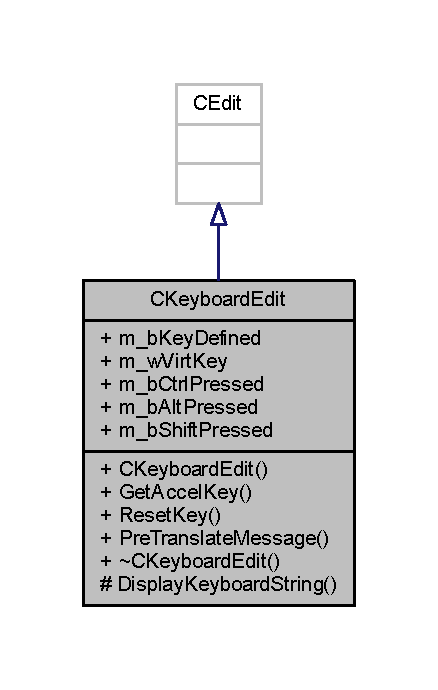
\includegraphics[width=210pt]{class_c_keyboard_edit__inherit__graph}
\end{center}
\end{figure}


C\+Keyboard\+Edit에 대한 협력 다이어그램\+:\nopagebreak
\begin{figure}[H]
\begin{center}
\leavevmode
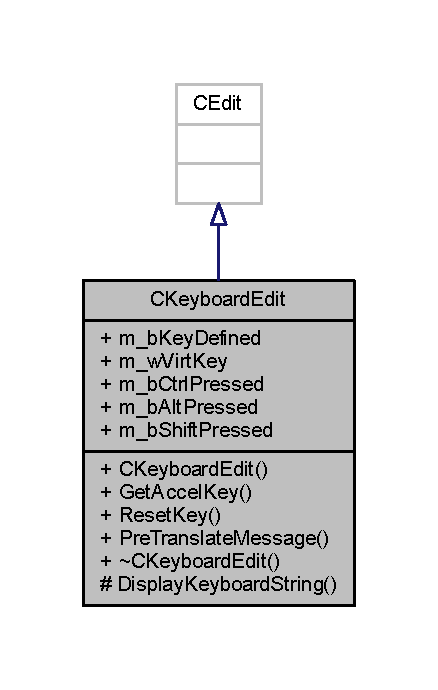
\includegraphics[width=210pt]{class_c_keyboard_edit__coll__graph}
\end{center}
\end{figure}
\subsection*{Public 멤버 함수}
\begin{DoxyCompactItemize}
\item 
\mbox{\hyperlink{class_c_keyboard_edit_a1a1165204f7f3bbfbd997c8cc94c97f8}{C\+Keyboard\+Edit}} ()
\item 
bool \mbox{\hyperlink{class_c_keyboard_edit_a920dfccebef5e2260e59003e4959ef9f}{Get\+Accel\+Key}} (W\+O\+RD \&w\+Virt\+Key, bool \&b\+Ctrl, bool \&b\+Alt, bool \&b\+Shift)
\item 
void \mbox{\hyperlink{class_c_keyboard_edit_ad0185cc0cad77250cc32ef1d9ffb8593}{Reset\+Key}} ()
\item 
virtual B\+O\+OL \mbox{\hyperlink{class_c_keyboard_edit_a7700247028b07400adf5056c6627e19a}{Pre\+Translate\+Message}} (\mbox{\hyperlink{prof_8cpp_a0c719c414608ef14852670b063876c07}{M\+SG}} $\ast$p\+Msg)
\item 
virtual \mbox{\hyperlink{class_c_keyboard_edit_aeddf780fee33d17188b5641cd384ab92}{$\sim$\+C\+Keyboard\+Edit}} ()
\end{DoxyCompactItemize}
\subsection*{Public 속성}
\begin{DoxyCompactItemize}
\item 
bool \mbox{\hyperlink{class_c_keyboard_edit_a9bf24703c8d1a3a019b43dc67c26c3a0}{m\+\_\+b\+Key\+Defined}}
\item 
W\+O\+RD \mbox{\hyperlink{class_c_keyboard_edit_a6a4efef92e151002720d0d930db29521}{m\+\_\+w\+Virt\+Key}}
\item 
bool \mbox{\hyperlink{class_c_keyboard_edit_a0dbb417bbaaeaa95c00fceaecd210064}{m\+\_\+b\+Ctrl\+Pressed}}
\item 
bool \mbox{\hyperlink{class_c_keyboard_edit_a724b035848eeca7bebc24e1309afeb6d}{m\+\_\+b\+Alt\+Pressed}}
\item 
bool \mbox{\hyperlink{class_c_keyboard_edit_ac4a4f45be9ef923961ab92a48a28f789}{m\+\_\+b\+Shift\+Pressed}}
\end{DoxyCompactItemize}
\subsection*{Protected 멤버 함수}
\begin{DoxyCompactItemize}
\item 
void \mbox{\hyperlink{class_c_keyboard_edit_a432e346d4d5285064b5e92ff4c6a0385}{Display\+Keyboard\+String}} ()
\end{DoxyCompactItemize}


\subsection{상세한 설명}


Keyboard\+Edit.\+h 파일의 40 번째 라인에서 정의되었습니다.



\subsection{생성자 \& 소멸자 문서화}
\mbox{\Hypertarget{class_c_keyboard_edit_a1a1165204f7f3bbfbd997c8cc94c97f8}\label{class_c_keyboard_edit_a1a1165204f7f3bbfbd997c8cc94c97f8}} 
\index{C\+Keyboard\+Edit@{C\+Keyboard\+Edit}!C\+Keyboard\+Edit@{C\+Keyboard\+Edit}}
\index{C\+Keyboard\+Edit@{C\+Keyboard\+Edit}!C\+Keyboard\+Edit@{C\+Keyboard\+Edit}}
\subsubsection{\texorpdfstring{C\+Keyboard\+Edit()}{CKeyboardEdit()}}
{\footnotesize\ttfamily C\+Keyboard\+Edit\+::\+C\+Keyboard\+Edit (\begin{DoxyParamCaption}{ }\end{DoxyParamCaption})}



Keyboard\+Edit.\+cpp 파일의 43 번째 라인에서 정의되었습니다.


\begin{DoxyCode}
44 \{
45   \mbox{\hyperlink{class_c_keyboard_edit_a9bf24703c8d1a3a019b43dc67c26c3a0}{m\_bKeyDefined}} = \textcolor{keyword}{false};
46   \mbox{\hyperlink{class_c_keyboard_edit_ad0185cc0cad77250cc32ef1d9ffb8593}{ResetKey}} ();
47 \}
\end{DoxyCode}
이 함수 내부에서 호출하는 함수들에 대한 그래프입니다.\+:
\nopagebreak
\begin{figure}[H]
\begin{center}
\leavevmode
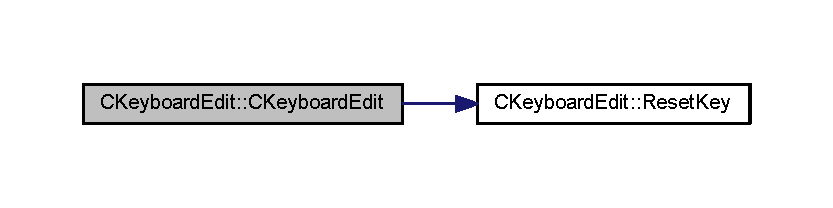
\includegraphics[width=350pt]{class_c_keyboard_edit_a1a1165204f7f3bbfbd997c8cc94c97f8_cgraph}
\end{center}
\end{figure}
\mbox{\Hypertarget{class_c_keyboard_edit_aeddf780fee33d17188b5641cd384ab92}\label{class_c_keyboard_edit_aeddf780fee33d17188b5641cd384ab92}} 
\index{C\+Keyboard\+Edit@{C\+Keyboard\+Edit}!````~C\+Keyboard\+Edit@{$\sim$\+C\+Keyboard\+Edit}}
\index{````~C\+Keyboard\+Edit@{$\sim$\+C\+Keyboard\+Edit}!C\+Keyboard\+Edit@{C\+Keyboard\+Edit}}
\subsubsection{\texorpdfstring{$\sim$\+C\+Keyboard\+Edit()}{~CKeyboardEdit()}}
{\footnotesize\ttfamily C\+Keyboard\+Edit\+::$\sim$\+C\+Keyboard\+Edit (\begin{DoxyParamCaption}{ }\end{DoxyParamCaption})\hspace{0.3cm}{\ttfamily [virtual]}}



Keyboard\+Edit.\+cpp 파일의 49 번째 라인에서 정의되었습니다.


\begin{DoxyCode}
50 \{
51 \}
\end{DoxyCode}


\subsection{멤버 함수 문서화}
\mbox{\Hypertarget{class_c_keyboard_edit_a432e346d4d5285064b5e92ff4c6a0385}\label{class_c_keyboard_edit_a432e346d4d5285064b5e92ff4c6a0385}} 
\index{C\+Keyboard\+Edit@{C\+Keyboard\+Edit}!Display\+Keyboard\+String@{Display\+Keyboard\+String}}
\index{Display\+Keyboard\+String@{Display\+Keyboard\+String}!C\+Keyboard\+Edit@{C\+Keyboard\+Edit}}
\subsubsection{\texorpdfstring{Display\+Keyboard\+String()}{DisplayKeyboardString()}}
{\footnotesize\ttfamily void C\+Keyboard\+Edit\+::\+Display\+Keyboard\+String (\begin{DoxyParamCaption}{ }\end{DoxyParamCaption})\hspace{0.3cm}{\ttfamily [protected]}}



Keyboard\+Edit.\+cpp 파일의 92 번째 라인에서 정의되었습니다.


\begin{DoxyCode}
93 \{
94   CString strKbd;
95 
96   \textcolor{comment}{// modifiers}
97   \textcolor{keywordflow}{if} (\mbox{\hyperlink{class_c_keyboard_edit_a0dbb417bbaaeaa95c00fceaecd210064}{m\_bCtrlPressed}})
98     strKbd = \textcolor{stringliteral}{"Ctrl"};
99   \textcolor{keywordflow}{if} (\mbox{\hyperlink{class_c_keyboard_edit_a724b035848eeca7bebc24e1309afeb6d}{m\_bAltPressed}}) \{
100     \textcolor{keywordflow}{if} (strKbd.GetLength () > 0)
101       strKbd += \textcolor{charliteral}{'+'};
102     strKbd += \textcolor{stringliteral}{"Alt"};
103   \}
104   \textcolor{keywordflow}{if} (\mbox{\hyperlink{class_c_keyboard_edit_ac4a4f45be9ef923961ab92a48a28f789}{m\_bShiftPressed}}) \{
105     \textcolor{keywordflow}{if} (strKbd.GetLength () > 0)
106       strKbd += \textcolor{charliteral}{'+'};
107     strKbd += \textcolor{stringliteral}{"Shift"};
108   \}
109   \textcolor{comment}{// virtual key}
110   LPCTSTR szVirtKey = \mbox{\hyperlink{_keyboard_edit_8cpp_a114f9fd0dc48511b3d2799f967360087}{mapVirtKeysStringFromWORD}}(
      \mbox{\hyperlink{class_c_keyboard_edit_a6a4efef92e151002720d0d930db29521}{m\_wVirtKey}});
111   \textcolor{keywordflow}{if} (szVirtKey != \mbox{\hyperlink{getopt1_8c_a070d2ce7b6bb7e5c05602aa8c308d0c4}{NULL}}) \{
112     \textcolor{keywordflow}{if} (strKbd.GetLength () > 0)
113       strKbd += \textcolor{charliteral}{'+'};
114     strKbd += szVirtKey;
115   \}
116   SetWindowText (strKbd);
117 \}
\end{DoxyCode}
이 함수 내부에서 호출하는 함수들에 대한 그래프입니다.\+:
\nopagebreak
\begin{figure}[H]
\begin{center}
\leavevmode
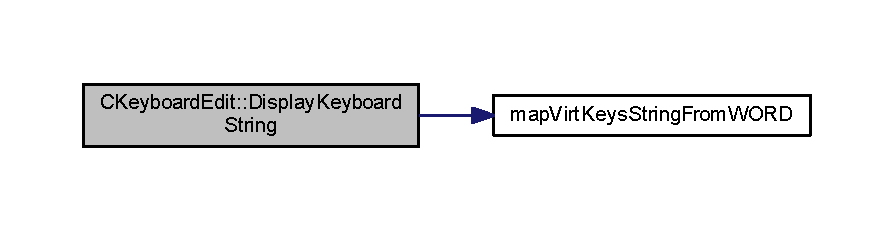
\includegraphics[width=350pt]{class_c_keyboard_edit_a432e346d4d5285064b5e92ff4c6a0385_cgraph}
\end{center}
\end{figure}
이 함수를 호출하는 함수들에 대한 그래프입니다.\+:
\nopagebreak
\begin{figure}[H]
\begin{center}
\leavevmode
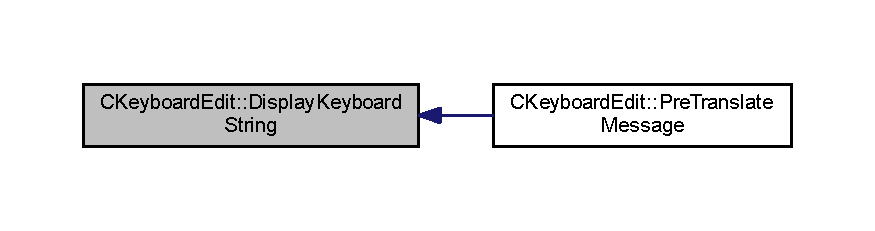
\includegraphics[width=350pt]{class_c_keyboard_edit_a432e346d4d5285064b5e92ff4c6a0385_icgraph}
\end{center}
\end{figure}
\mbox{\Hypertarget{class_c_keyboard_edit_a920dfccebef5e2260e59003e4959ef9f}\label{class_c_keyboard_edit_a920dfccebef5e2260e59003e4959ef9f}} 
\index{C\+Keyboard\+Edit@{C\+Keyboard\+Edit}!Get\+Accel\+Key@{Get\+Accel\+Key}}
\index{Get\+Accel\+Key@{Get\+Accel\+Key}!C\+Keyboard\+Edit@{C\+Keyboard\+Edit}}
\subsubsection{\texorpdfstring{Get\+Accel\+Key()}{GetAccelKey()}}
{\footnotesize\ttfamily bool C\+Keyboard\+Edit\+::\+Get\+Accel\+Key (\begin{DoxyParamCaption}\item[{W\+O\+RD \&}]{w\+Virt\+Key,  }\item[{bool \&}]{b\+Ctrl,  }\item[{bool \&}]{b\+Alt,  }\item[{bool \&}]{b\+Shift }\end{DoxyParamCaption})}



Keyboard\+Edit.\+cpp 파일의 137 번째 라인에서 정의되었습니다.


\begin{DoxyCode}
138 \{
139   \textcolor{keywordflow}{if} (!\mbox{\hyperlink{class_c_keyboard_edit_a9bf24703c8d1a3a019b43dc67c26c3a0}{m\_bKeyDefined}})
140     \textcolor{keywordflow}{return} \textcolor{keyword}{false};
141   
142   wVirtKey = \mbox{\hyperlink{class_c_keyboard_edit_a6a4efef92e151002720d0d930db29521}{m\_wVirtKey}};
143   bAlt = \mbox{\hyperlink{class_c_keyboard_edit_a724b035848eeca7bebc24e1309afeb6d}{m\_bAltPressed}};
144   bCtrl = \mbox{\hyperlink{class_c_keyboard_edit_a0dbb417bbaaeaa95c00fceaecd210064}{m\_bCtrlPressed}};
145   bShift = \mbox{\hyperlink{class_c_keyboard_edit_ac4a4f45be9ef923961ab92a48a28f789}{m\_bShiftPressed}};
146   \textcolor{keywordflow}{return} \textcolor{keyword}{true};
147 \}
\end{DoxyCode}
이 함수를 호출하는 함수들에 대한 그래프입니다.\+:
\nopagebreak
\begin{figure}[H]
\begin{center}
\leavevmode
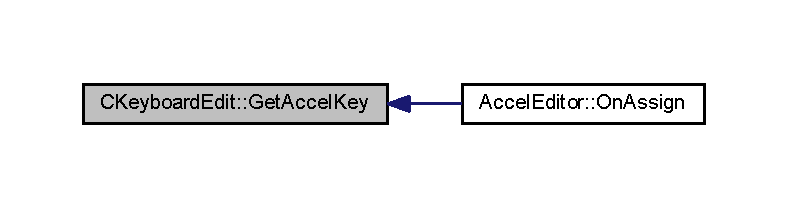
\includegraphics[width=350pt]{class_c_keyboard_edit_a920dfccebef5e2260e59003e4959ef9f_icgraph}
\end{center}
\end{figure}
\mbox{\Hypertarget{class_c_keyboard_edit_a7700247028b07400adf5056c6627e19a}\label{class_c_keyboard_edit_a7700247028b07400adf5056c6627e19a}} 
\index{C\+Keyboard\+Edit@{C\+Keyboard\+Edit}!Pre\+Translate\+Message@{Pre\+Translate\+Message}}
\index{Pre\+Translate\+Message@{Pre\+Translate\+Message}!C\+Keyboard\+Edit@{C\+Keyboard\+Edit}}
\subsubsection{\texorpdfstring{Pre\+Translate\+Message()}{PreTranslateMessage()}}
{\footnotesize\ttfamily B\+O\+OL C\+Keyboard\+Edit\+::\+Pre\+Translate\+Message (\begin{DoxyParamCaption}\item[{\mbox{\hyperlink{prof_8cpp_a0c719c414608ef14852670b063876c07}{M\+SG}} $\ast$}]{p\+Msg }\end{DoxyParamCaption})\hspace{0.3cm}{\ttfamily [virtual]}}



Keyboard\+Edit.\+cpp 파일의 62 번째 라인에서 정의되었습니다.


\begin{DoxyCode}
63 \{
64   \textcolor{keywordtype}{bool} bPressed;
65   \textcolor{keywordflow}{if} ((bPressed = (pMsg->message == WM\_KEYDOWN)) || pMsg->message == WM\_KEYUP || (bPressed = (pMsg->message
       == WM\_SYSKEYDOWN)) || pMsg->message == WM\_SYSKEYUP) \{
66     \textcolor{keywordflow}{if} (bPressed && \mbox{\hyperlink{class_c_keyboard_edit_a9bf24703c8d1a3a019b43dc67c26c3a0}{m\_bKeyDefined}} && !((1 << 30) & pMsg->lParam))
67       \mbox{\hyperlink{class_c_keyboard_edit_ad0185cc0cad77250cc32ef1d9ffb8593}{ResetKey}} ();
68     \textcolor{keywordflow}{if} (pMsg->wParam == VK\_SHIFT && !\mbox{\hyperlink{class_c_keyboard_edit_a9bf24703c8d1a3a019b43dc67c26c3a0}{m\_bKeyDefined}})
69       \mbox{\hyperlink{class_c_keyboard_edit_ac4a4f45be9ef923961ab92a48a28f789}{m\_bShiftPressed}} = bPressed;
70     \textcolor{keywordflow}{else} \textcolor{keywordflow}{if} (pMsg->wParam == VK\_CONTROL &&!\mbox{\hyperlink{class_c_keyboard_edit_a9bf24703c8d1a3a019b43dc67c26c3a0}{m\_bKeyDefined}}) \{
71       \mbox{\hyperlink{class_c_keyboard_edit_a0dbb417bbaaeaa95c00fceaecd210064}{m\_bCtrlPressed}} = bPressed;
72     \}
73     \textcolor{keywordflow}{else} \textcolor{keywordflow}{if} (pMsg->wParam == VK\_MENU && !\mbox{\hyperlink{class_c_keyboard_edit_a9bf24703c8d1a3a019b43dc67c26c3a0}{m\_bKeyDefined}})
74       \mbox{\hyperlink{class_c_keyboard_edit_a724b035848eeca7bebc24e1309afeb6d}{m\_bAltPressed}} = bPressed;
75     \textcolor{keywordflow}{else} \{
76       \textcolor{keywordflow}{if} (!\mbox{\hyperlink{class_c_keyboard_edit_a9bf24703c8d1a3a019b43dc67c26c3a0}{m\_bKeyDefined}}) \{
77         \mbox{\hyperlink{class_c_keyboard_edit_a6a4efef92e151002720d0d930db29521}{m\_wVirtKey}} = (WORD)pMsg->wParam;
78         \mbox{\hyperlink{arm-new_8h_a93120066fd6daa54150af823953378d1}{if}} (bPressed)
79           \mbox{\hyperlink{class_c_keyboard_edit_a9bf24703c8d1a3a019b43dc67c26c3a0}{m\_bKeyDefined}} = \textcolor{keyword}{true};
80       \}
81     \}
82     \mbox{\hyperlink{class_c_keyboard_edit_a432e346d4d5285064b5e92ff4c6a0385}{DisplayKeyboardString}} ();
83     \textcolor{keywordflow}{return} TRUE;
84   \}
85         
86   \textcolor{keywordflow}{return} CEdit::PreTranslateMessage(pMsg);
87 \}
\end{DoxyCode}
이 함수 내부에서 호출하는 함수들에 대한 그래프입니다.\+:
\nopagebreak
\begin{figure}[H]
\begin{center}
\leavevmode
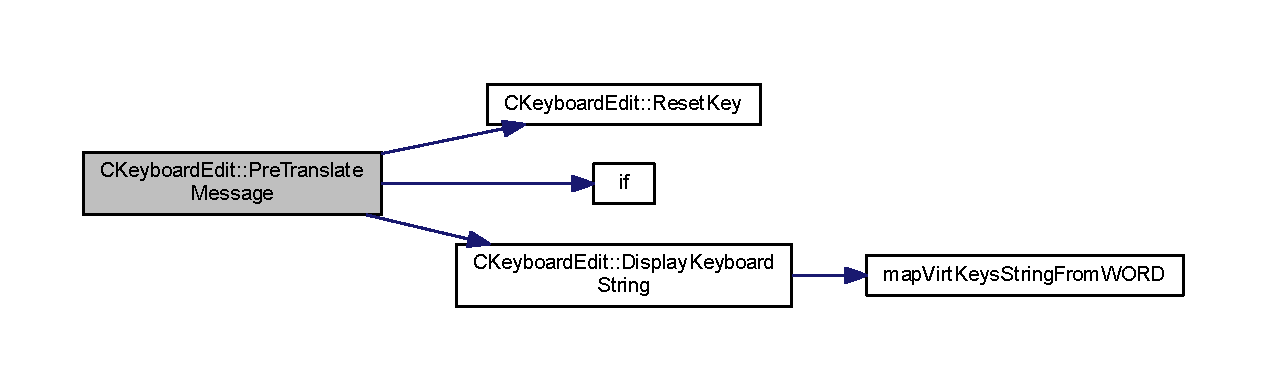
\includegraphics[width=350pt]{class_c_keyboard_edit_a7700247028b07400adf5056c6627e19a_cgraph}
\end{center}
\end{figure}
\mbox{\Hypertarget{class_c_keyboard_edit_ad0185cc0cad77250cc32ef1d9ffb8593}\label{class_c_keyboard_edit_ad0185cc0cad77250cc32ef1d9ffb8593}} 
\index{C\+Keyboard\+Edit@{C\+Keyboard\+Edit}!Reset\+Key@{Reset\+Key}}
\index{Reset\+Key@{Reset\+Key}!C\+Keyboard\+Edit@{C\+Keyboard\+Edit}}
\subsubsection{\texorpdfstring{Reset\+Key()}{ResetKey()}}
{\footnotesize\ttfamily void C\+Keyboard\+Edit\+::\+Reset\+Key (\begin{DoxyParamCaption}{ }\end{DoxyParamCaption})}



Keyboard\+Edit.\+cpp 파일의 122 번째 라인에서 정의되었습니다.


\begin{DoxyCode}
123 \{
124   \mbox{\hyperlink{class_c_keyboard_edit_a6a4efef92e151002720d0d930db29521}{m\_wVirtKey}} = 0;
125   \mbox{\hyperlink{class_c_keyboard_edit_a0dbb417bbaaeaa95c00fceaecd210064}{m\_bCtrlPressed}} = \textcolor{keyword}{false};
126   \mbox{\hyperlink{class_c_keyboard_edit_a724b035848eeca7bebc24e1309afeb6d}{m\_bAltPressed}} = \textcolor{keyword}{false};
127   \mbox{\hyperlink{class_c_keyboard_edit_ac4a4f45be9ef923961ab92a48a28f789}{m\_bShiftPressed}} = \textcolor{keyword}{false};
128   
129   \mbox{\hyperlink{class_c_keyboard_edit_a9bf24703c8d1a3a019b43dc67c26c3a0}{m\_bKeyDefined}} = \textcolor{keyword}{false};
130   \textcolor{keywordflow}{if}(m\_hWnd != \mbox{\hyperlink{getopt1_8c_a070d2ce7b6bb7e5c05602aa8c308d0c4}{NULL}})
131     SetWindowText(\_T(\textcolor{stringliteral}{""}));
132 \}
\end{DoxyCode}
이 함수를 호출하는 함수들에 대한 그래프입니다.\+:
\nopagebreak
\begin{figure}[H]
\begin{center}
\leavevmode
\includegraphics[width=350pt]{class_c_keyboard_edit_ad0185cc0cad77250cc32ef1d9ffb8593_icgraph}
\end{center}
\end{figure}


\subsection{멤버 데이터 문서화}
\mbox{\Hypertarget{class_c_keyboard_edit_a724b035848eeca7bebc24e1309afeb6d}\label{class_c_keyboard_edit_a724b035848eeca7bebc24e1309afeb6d}} 
\index{C\+Keyboard\+Edit@{C\+Keyboard\+Edit}!m\+\_\+b\+Alt\+Pressed@{m\+\_\+b\+Alt\+Pressed}}
\index{m\+\_\+b\+Alt\+Pressed@{m\+\_\+b\+Alt\+Pressed}!C\+Keyboard\+Edit@{C\+Keyboard\+Edit}}
\subsubsection{\texorpdfstring{m\+\_\+b\+Alt\+Pressed}{m\_bAltPressed}}
{\footnotesize\ttfamily bool C\+Keyboard\+Edit\+::m\+\_\+b\+Alt\+Pressed}



Keyboard\+Edit.\+h 파일의 52 번째 라인에서 정의되었습니다.

\mbox{\Hypertarget{class_c_keyboard_edit_a0dbb417bbaaeaa95c00fceaecd210064}\label{class_c_keyboard_edit_a0dbb417bbaaeaa95c00fceaecd210064}} 
\index{C\+Keyboard\+Edit@{C\+Keyboard\+Edit}!m\+\_\+b\+Ctrl\+Pressed@{m\+\_\+b\+Ctrl\+Pressed}}
\index{m\+\_\+b\+Ctrl\+Pressed@{m\+\_\+b\+Ctrl\+Pressed}!C\+Keyboard\+Edit@{C\+Keyboard\+Edit}}
\subsubsection{\texorpdfstring{m\+\_\+b\+Ctrl\+Pressed}{m\_bCtrlPressed}}
{\footnotesize\ttfamily bool C\+Keyboard\+Edit\+::m\+\_\+b\+Ctrl\+Pressed}



Keyboard\+Edit.\+h 파일의 51 번째 라인에서 정의되었습니다.

\mbox{\Hypertarget{class_c_keyboard_edit_a9bf24703c8d1a3a019b43dc67c26c3a0}\label{class_c_keyboard_edit_a9bf24703c8d1a3a019b43dc67c26c3a0}} 
\index{C\+Keyboard\+Edit@{C\+Keyboard\+Edit}!m\+\_\+b\+Key\+Defined@{m\+\_\+b\+Key\+Defined}}
\index{m\+\_\+b\+Key\+Defined@{m\+\_\+b\+Key\+Defined}!C\+Keyboard\+Edit@{C\+Keyboard\+Edit}}
\subsubsection{\texorpdfstring{m\+\_\+b\+Key\+Defined}{m\_bKeyDefined}}
{\footnotesize\ttfamily bool C\+Keyboard\+Edit\+::m\+\_\+b\+Key\+Defined}



Keyboard\+Edit.\+h 파일의 48 번째 라인에서 정의되었습니다.

\mbox{\Hypertarget{class_c_keyboard_edit_ac4a4f45be9ef923961ab92a48a28f789}\label{class_c_keyboard_edit_ac4a4f45be9ef923961ab92a48a28f789}} 
\index{C\+Keyboard\+Edit@{C\+Keyboard\+Edit}!m\+\_\+b\+Shift\+Pressed@{m\+\_\+b\+Shift\+Pressed}}
\index{m\+\_\+b\+Shift\+Pressed@{m\+\_\+b\+Shift\+Pressed}!C\+Keyboard\+Edit@{C\+Keyboard\+Edit}}
\subsubsection{\texorpdfstring{m\+\_\+b\+Shift\+Pressed}{m\_bShiftPressed}}
{\footnotesize\ttfamily bool C\+Keyboard\+Edit\+::m\+\_\+b\+Shift\+Pressed}



Keyboard\+Edit.\+h 파일의 53 번째 라인에서 정의되었습니다.

\mbox{\Hypertarget{class_c_keyboard_edit_a6a4efef92e151002720d0d930db29521}\label{class_c_keyboard_edit_a6a4efef92e151002720d0d930db29521}} 
\index{C\+Keyboard\+Edit@{C\+Keyboard\+Edit}!m\+\_\+w\+Virt\+Key@{m\+\_\+w\+Virt\+Key}}
\index{m\+\_\+w\+Virt\+Key@{m\+\_\+w\+Virt\+Key}!C\+Keyboard\+Edit@{C\+Keyboard\+Edit}}
\subsubsection{\texorpdfstring{m\+\_\+w\+Virt\+Key}{m\_wVirtKey}}
{\footnotesize\ttfamily W\+O\+RD C\+Keyboard\+Edit\+::m\+\_\+w\+Virt\+Key}



Keyboard\+Edit.\+h 파일의 50 번째 라인에서 정의되었습니다.



이 클래스에 대한 문서화 페이지는 다음의 파일들로부터 생성되었습니다.\+:\begin{DoxyCompactItemize}
\item 
C\+:/\+Users/sjh13/sources/\+Visual\+Boy\+Advance/src/win32/\mbox{\hyperlink{_keyboard_edit_8h}{Keyboard\+Edit.\+h}}\item 
C\+:/\+Users/sjh13/sources/\+Visual\+Boy\+Advance/src/win32/\mbox{\hyperlink{_keyboard_edit_8cpp}{Keyboard\+Edit.\+cpp}}\end{DoxyCompactItemize}

\hypertarget{class_win_helper_1_1_c_critical_section_1_1_c_lock}{}\section{Win\+Helper\+:\+:C\+Critical\+Section\+:\+:C\+Lock 클래스 참조}
\label{class_win_helper_1_1_c_critical_section_1_1_c_lock}\index{Win\+Helper\+::\+C\+Critical\+Section\+::\+C\+Lock@{Win\+Helper\+::\+C\+Critical\+Section\+::\+C\+Lock}}
\subsection*{Public 멤버 함수}
\begin{DoxyCompactItemize}
\item 
\mbox{\Hypertarget{class_win_helper_1_1_c_critical_section_1_1_c_lock_a68cee1cb129d83775f678a4bde96c049}\label{class_win_helper_1_1_c_critical_section_1_1_c_lock_a68cee1cb129d83775f678a4bde96c049}} 
{\bfseries C\+Lock} (\mbox{\hyperlink{class_win_helper_1_1_c_critical_section}{C\+Critical\+Section}} \&sect)
\end{DoxyCompactItemize}


이 클래스에 대한 문서화 페이지는 다음의 파일로부터 생성되었습니다.\+:\begin{DoxyCompactItemize}
\item 
src/win32/Win\+Helper.\+h\end{DoxyCompactItemize}

\hypertarget{class_color_button}{}\section{Color\+Button 클래스 참조}
\label{class_color_button}\index{Color\+Button@{Color\+Button}}


{\ttfamily \#include $<$Color\+Button.\+h$>$}



Color\+Button에 대한 상속 다이어그램 \+: \nopagebreak
\begin{figure}[H]
\begin{center}
\leavevmode
\includegraphics[width=202pt]{class_color_button__inherit__graph}
\end{center}
\end{figure}


Color\+Button에 대한 협력 다이어그램\+:\nopagebreak
\begin{figure}[H]
\begin{center}
\leavevmode
\includegraphics[width=202pt]{class_color_button__coll__graph}
\end{center}
\end{figure}
\subsection*{Public 멤버 함수}
\begin{DoxyCompactItemize}
\item 
\mbox{\hyperlink{class_color_button_a4b8e318941c5c69efd5a610fd7edb51e}{Color\+Button}} ()
\item 
void \mbox{\hyperlink{class_color_button_a2252acea0c111e198cc5bcc914e2cfeb}{Pre\+Subclass\+Window}} ()
\item 
void \mbox{\hyperlink{class_color_button_a48b973ebb6644f474f64ff1e8fbb1adf}{Draw\+Item}} (L\+P\+D\+R\+A\+W\+I\+T\+E\+M\+S\+T\+R\+U\+CT lp\+Draw\+Item\+Struct)
\item 
void \mbox{\hyperlink{class_color_button_a9ff5dc144a4acd5e2551ab94506b3bb0}{set\+Color}} (\mbox{\hyperlink{_system_8h_a9e6c91d77e24643b888dbd1a1a590054}{u16}} c)
\item 
virtual \mbox{\hyperlink{class_color_button_a992ff40e28cd869985afcf02ef338797}{$\sim$\+Color\+Button}} ()
\item 
void \mbox{\hyperlink{class_color_button_aabbc7306d4354479e0315b2a15026571}{register\+Class}} ()
\end{DoxyCompactItemize}
\subsection*{Public 속성}
\begin{DoxyCompactItemize}
\item 
\mbox{\hyperlink{_system_8h_a9e6c91d77e24643b888dbd1a1a590054}{u16}} \mbox{\hyperlink{class_color_button_ac2e59577aba7413fbf40c97f21df4835}{color}}
\end{DoxyCompactItemize}
\subsection*{정적 Public 속성}
\begin{DoxyCompactItemize}
\item 
static bool \mbox{\hyperlink{class_color_button_a77e2fa25affb19cac1c18594d5bc478f}{is\+Registered}} = false
\end{DoxyCompactItemize}


\subsection{상세한 설명}


Color\+Button.\+h 파일의 33 번째 라인에서 정의되었습니다.



\subsection{생성자 \& 소멸자 문서화}
\mbox{\Hypertarget{class_color_button_a4b8e318941c5c69efd5a610fd7edb51e}\label{class_color_button_a4b8e318941c5c69efd5a610fd7edb51e}} 
\index{Color\+Button@{Color\+Button}!Color\+Button@{Color\+Button}}
\index{Color\+Button@{Color\+Button}!Color\+Button@{Color\+Button}}
\subsubsection{\texorpdfstring{Color\+Button()}{ColorButton()}}
{\footnotesize\ttfamily Color\+Button\+::\+Color\+Button (\begin{DoxyParamCaption}{ }\end{DoxyParamCaption})}



Color\+Button.\+cpp 파일의 37 번째 라인에서 정의되었습니다.


\begin{DoxyCode}
38 \{
39   \mbox{\hyperlink{class_color_button_ac2e59577aba7413fbf40c97f21df4835}{color}} = 0;
40   \mbox{\hyperlink{class_color_button_aabbc7306d4354479e0315b2a15026571}{registerClass}}();
41 \}
\end{DoxyCode}
이 함수 내부에서 호출하는 함수들에 대한 그래프입니다.\+:
\nopagebreak
\begin{figure}[H]
\begin{center}
\leavevmode
\includegraphics[width=350pt]{class_color_button_a4b8e318941c5c69efd5a610fd7edb51e_cgraph}
\end{center}
\end{figure}
\mbox{\Hypertarget{class_color_button_a992ff40e28cd869985afcf02ef338797}\label{class_color_button_a992ff40e28cd869985afcf02ef338797}} 
\index{Color\+Button@{Color\+Button}!````~Color\+Button@{$\sim$\+Color\+Button}}
\index{````~Color\+Button@{$\sim$\+Color\+Button}!Color\+Button@{Color\+Button}}
\subsubsection{\texorpdfstring{$\sim$\+Color\+Button()}{~ColorButton()}}
{\footnotesize\ttfamily Color\+Button\+::$\sim$\+Color\+Button (\begin{DoxyParamCaption}{ }\end{DoxyParamCaption})\hspace{0.3cm}{\ttfamily [virtual]}}



Color\+Button.\+cpp 파일의 43 번째 라인에서 정의되었습니다.


\begin{DoxyCode}
44 \{
45 \}
\end{DoxyCode}


\subsection{멤버 함수 문서화}
\mbox{\Hypertarget{class_color_button_a48b973ebb6644f474f64ff1e8fbb1adf}\label{class_color_button_a48b973ebb6644f474f64ff1e8fbb1adf}} 
\index{Color\+Button@{Color\+Button}!Draw\+Item@{Draw\+Item}}
\index{Draw\+Item@{Draw\+Item}!Color\+Button@{Color\+Button}}
\subsubsection{\texorpdfstring{Draw\+Item()}{DrawItem()}}
{\footnotesize\ttfamily void Color\+Button\+::\+Draw\+Item (\begin{DoxyParamCaption}\item[{L\+P\+D\+R\+A\+W\+I\+T\+E\+M\+S\+T\+R\+U\+CT}]{lp\+Draw\+Item\+Struct }\end{DoxyParamCaption})}



Color\+Button.\+cpp 파일의 63 번째 라인에서 정의되었습니다.


\begin{DoxyCode}
64 \{
65   ASSERT(lpDrawItemStruct);
66   
67   \textcolor{keywordtype}{int} r = (\mbox{\hyperlink{class_color_button_ac2e59577aba7413fbf40c97f21df4835}{color}} & 0x1f) << 3;
68   \textcolor{keywordtype}{int} g = (\mbox{\hyperlink{class_color_button_ac2e59577aba7413fbf40c97f21df4835}{color}} & 0x3e0) >> 2;
69   \textcolor{keywordtype}{int} \mbox{\hyperlink{expr-lex_8cpp_a91b64995742fd30063314f12340b4b5a}{b}} = (\mbox{\hyperlink{class_color_button_ac2e59577aba7413fbf40c97f21df4835}{color}} & 0x7c00) >> 7;
70 
71   HDC dc = lpDrawItemStruct->hDC;
72   UINT state = lpDrawItemStruct->itemState;
73   RECT rect = lpDrawItemStruct->rcItem;
74 
75   SIZE margins;
76   margins.cx = ::GetSystemMetrics(SM\_CXEDGE);
77   margins.cy = ::GetSystemMetrics(SM\_CYEDGE);
78 
79   \textcolor{keywordflow}{if}(GetState() & BST\_PUSHED)
80     DrawEdge(dc, &rect, EDGE\_SUNKEN, BF\_RECT);
81   \textcolor{keywordflow}{else}
82     DrawEdge(dc, &rect, EDGE\_RAISED, BF\_RECT);
83 
84   InflateRect(&rect, -margins.cx, -margins.cy);
85   
86   HBRUSH br = CreateSolidBrush((state & ODS\_DISABLED) ? 
87                                ::GetSysColor(COLOR\_3DFACE) : \mbox{\hyperlink{bilinear_8cpp_a4a118ad3ee36468a3fa616977a64864e}{RGB}}(r,g,\mbox{\hyperlink{expr-lex_8cpp_a91b64995742fd30063314f12340b4b5a}{b}}));
88 
89   FillRect(dc, &rect, br);
90 
91   \textcolor{keywordflow}{if}(state & ODS\_FOCUS) \{
92     InflateRect(&rect, -1, -1);
93     DrawFocusRect(dc, &rect);
94   \}
95   
96   DeleteObject(br);
97 \}
\end{DoxyCode}
\mbox{\Hypertarget{class_color_button_a2252acea0c111e198cc5bcc914e2cfeb}\label{class_color_button_a2252acea0c111e198cc5bcc914e2cfeb}} 
\index{Color\+Button@{Color\+Button}!Pre\+Subclass\+Window@{Pre\+Subclass\+Window}}
\index{Pre\+Subclass\+Window@{Pre\+Subclass\+Window}!Color\+Button@{Color\+Button}}
\subsubsection{\texorpdfstring{Pre\+Subclass\+Window()}{PreSubclassWindow()}}
{\footnotesize\ttfamily void Color\+Button\+::\+Pre\+Subclass\+Window (\begin{DoxyParamCaption}{ }\end{DoxyParamCaption})}



Color\+Button.\+cpp 파일의 57 번째 라인에서 정의되었습니다.


\begin{DoxyCode}
58 \{
59   SetWindowLong(m\_hWnd, GWL\_STYLE, GetStyle() | BS\_OWNERDRAW);
60   CWnd::PreSubclassWindow();
61 \}
\end{DoxyCode}
\mbox{\Hypertarget{class_color_button_aabbc7306d4354479e0315b2a15026571}\label{class_color_button_aabbc7306d4354479e0315b2a15026571}} 
\index{Color\+Button@{Color\+Button}!register\+Class@{register\+Class}}
\index{register\+Class@{register\+Class}!Color\+Button@{Color\+Button}}
\subsubsection{\texorpdfstring{register\+Class()}{registerClass()}}
{\footnotesize\ttfamily void Color\+Button\+::register\+Class (\begin{DoxyParamCaption}{ }\end{DoxyParamCaption})}



Color\+Button.\+cpp 파일의 105 번째 라인에서 정의되었습니다.


\begin{DoxyCode}
106 \{
107   \textcolor{keywordflow}{if}(!\mbox{\hyperlink{class_color_button_a77e2fa25affb19cac1c18594d5bc478f}{isRegistered}}) \{
108     WNDCLASS wc;
109     ZeroMemory(&wc, \textcolor{keyword}{sizeof}(wc));
110     wc.style = CS\_HREDRAW | CS\_VREDRAW | CS\_GLOBALCLASS;
111     wc.lpfnWndProc = (WNDPROC)::DefWindowProc;
112     wc.hInstance = AfxGetInstanceHandle();
113     wc.hIcon = LoadCursor(\mbox{\hyperlink{getopt1_8c_a070d2ce7b6bb7e5c05602aa8c308d0c4}{NULL}}, IDC\_ARROW);
114     wc.hbrBackground = (HBRUSH )GetStockObject(BLACK\_BRUSH);
115     wc.lpszMenuName = \mbox{\hyperlink{getopt1_8c_a070d2ce7b6bb7e5c05602aa8c308d0c4}{NULL}};
116     wc.lpszClassName = \textcolor{stringliteral}{"VbaColorButton"};
117     AfxRegisterClass(&wc);
118     \mbox{\hyperlink{class_color_button_a77e2fa25affb19cac1c18594d5bc478f}{isRegistered}} = \textcolor{keyword}{true};
119   \}
120 \}
\end{DoxyCode}
이 함수를 호출하는 함수들에 대한 그래프입니다.\+:
\nopagebreak
\begin{figure}[H]
\begin{center}
\leavevmode
\includegraphics[width=350pt]{class_color_button_aabbc7306d4354479e0315b2a15026571_icgraph}
\end{center}
\end{figure}
\mbox{\Hypertarget{class_color_button_a9ff5dc144a4acd5e2551ab94506b3bb0}\label{class_color_button_a9ff5dc144a4acd5e2551ab94506b3bb0}} 
\index{Color\+Button@{Color\+Button}!set\+Color@{set\+Color}}
\index{set\+Color@{set\+Color}!Color\+Button@{Color\+Button}}
\subsubsection{\texorpdfstring{set\+Color()}{setColor()}}
{\footnotesize\ttfamily void Color\+Button\+::set\+Color (\begin{DoxyParamCaption}\item[{\mbox{\hyperlink{_system_8h_a9e6c91d77e24643b888dbd1a1a590054}{u16}}}]{c }\end{DoxyParamCaption})}



Color\+Button.\+cpp 파일의 99 번째 라인에서 정의되었습니다.


\begin{DoxyCode}
100 \{
101   \mbox{\hyperlink{class_color_button_ac2e59577aba7413fbf40c97f21df4835}{color}} = c;
102   Invalidate();
103 \}
\end{DoxyCode}
이 함수를 호출하는 함수들에 대한 그래프입니다.\+:
\nopagebreak
\begin{figure}[H]
\begin{center}
\leavevmode
\includegraphics[width=350pt]{class_color_button_a9ff5dc144a4acd5e2551ab94506b3bb0_icgraph}
\end{center}
\end{figure}


\subsection{멤버 데이터 문서화}
\mbox{\Hypertarget{class_color_button_ac2e59577aba7413fbf40c97f21df4835}\label{class_color_button_ac2e59577aba7413fbf40c97f21df4835}} 
\index{Color\+Button@{Color\+Button}!color@{color}}
\index{color@{color}!Color\+Button@{Color\+Button}}
\subsubsection{\texorpdfstring{color}{color}}
{\footnotesize\ttfamily \mbox{\hyperlink{_system_8h_a9e6c91d77e24643b888dbd1a1a590054}{u16}} Color\+Button\+::color}



Color\+Button.\+h 파일의 55 번째 라인에서 정의되었습니다.

\mbox{\Hypertarget{class_color_button_a77e2fa25affb19cac1c18594d5bc478f}\label{class_color_button_a77e2fa25affb19cac1c18594d5bc478f}} 
\index{Color\+Button@{Color\+Button}!is\+Registered@{is\+Registered}}
\index{is\+Registered@{is\+Registered}!Color\+Button@{Color\+Button}}
\subsubsection{\texorpdfstring{is\+Registered}{isRegistered}}
{\footnotesize\ttfamily bool Color\+Button\+::is\+Registered = false\hspace{0.3cm}{\ttfamily [static]}}



Color\+Button.\+h 파일의 42 번째 라인에서 정의되었습니다.



이 클래스에 대한 문서화 페이지는 다음의 파일들로부터 생성되었습니다.\+:\begin{DoxyCompactItemize}
\item 
C\+:/\+Users/sjh13/sources/\+Visual\+Boy\+Advance/src/win32/\mbox{\hyperlink{_color_button_8h}{Color\+Button.\+h}}\item 
C\+:/\+Users/sjh13/sources/\+Visual\+Boy\+Advance/src/win32/\mbox{\hyperlink{_color_button_8cpp}{Color\+Button.\+cpp}}\end{DoxyCompactItemize}

\hypertarget{class_color_control}{}\section{Color\+Control 클래스 참조}
\label{class_color_control}\index{Color\+Control@{Color\+Control}}
Color\+Control에 대한 상속 다이어그램 \+: \begin{figure}[H]
\begin{center}
\leavevmode
\includegraphics[height=2.000000cm]{class_color_control}
\end{center}
\end{figure}
\subsection*{Public 멤버 함수}
\begin{DoxyCompactItemize}
\item 
\mbox{\Hypertarget{class_color_control_ad4f5b637e57ab4e7c4ed718e66e491eb}\label{class_color_control_ad4f5b637e57ab4e7c4ed718e66e491eb}} 
void {\bfseries set\+Color} (u16 c)
\end{DoxyCompactItemize}
\subsection*{Public 속성}
\begin{DoxyCompactItemize}
\item 
\mbox{\Hypertarget{class_color_control_adda78267113753c247e7edcaae47f927}\label{class_color_control_adda78267113753c247e7edcaae47f927}} 
u16 {\bfseries color}
\end{DoxyCompactItemize}
\subsection*{정적 Public 속성}
\begin{DoxyCompactItemize}
\item 
\mbox{\Hypertarget{class_color_control_a844b865ffc83cf76b50a3f7b0793619e}\label{class_color_control_a844b865ffc83cf76b50a3f7b0793619e}} 
static bool {\bfseries is\+Registered} = false
\end{DoxyCompactItemize}
\subsection*{Protected 멤버 함수}
\begin{DoxyCompactItemize}
\item 
\mbox{\Hypertarget{class_color_control_a63bcd96ef7044bf702632cab0fc41eba}\label{class_color_control_a63bcd96ef7044bf702632cab0fc41eba}} 
afx\+\_\+msg void {\bfseries On\+Paint} ()
\item 
\mbox{\Hypertarget{class_color_control_a06b4b2fd6e06aab248c7e63859ea4f11}\label{class_color_control_a06b4b2fd6e06aab248c7e63859ea4f11}} 
afx\+\_\+msg B\+O\+OL {\bfseries On\+Erase\+Bkgnd} (C\+DC $\ast$p\+DC)
\end{DoxyCompactItemize}


이 클래스에 대한 문서화 페이지는 다음의 파일들로부터 생성되었습니다.\+:\begin{DoxyCompactItemize}
\item 
src/win32/Color\+Control.\+h\item 
src/win32/Color\+Control.\+cpp\end{DoxyCompactItemize}

\hypertarget{struct_compile_unit}{}\section{Compile\+Unit 구조체 참조}
\label{struct_compile_unit}\index{Compile\+Unit@{Compile\+Unit}}


{\ttfamily \#include $<$elf.\+h$>$}



Compile\+Unit에 대한 협력 다이어그램\+:\nopagebreak
\begin{figure}[H]
\begin{center}
\leavevmode
\includegraphics[width=350pt]{struct_compile_unit__coll__graph}
\end{center}
\end{figure}
\subsection*{Public 속성}
\begin{DoxyCompactItemize}
\item 
\mbox{\hyperlink{_system_8h_a10e94b422ef0c20dcdec20d31a1f5049}{u32}} \mbox{\hyperlink{struct_compile_unit_acad6384874d710baa10548c0bf9a391a}{length}}
\item 
\mbox{\hyperlink{_system_8h_aed742c436da53c1080638ce6ef7d13de}{u8}} $\ast$ \mbox{\hyperlink{struct_compile_unit_ace3ba5846b6ef2bce6fb6ecf08cad32f}{top}}
\item 
\mbox{\hyperlink{_system_8h_a10e94b422ef0c20dcdec20d31a1f5049}{u32}} \mbox{\hyperlink{struct_compile_unit_a25babc3939d9beaf5f9fb713b06d7ff0}{offset}}
\item 
\mbox{\hyperlink{struct_e_l_f_abbrev}{E\+L\+F\+Abbrev}} $\ast$$\ast$ \mbox{\hyperlink{struct_compile_unit_a53e5f3d3a9863efd87c6bc56de6a8ede}{abbrevs}}
\item 
\mbox{\hyperlink{struct_a_ranges}{A\+Ranges}} $\ast$ \mbox{\hyperlink{struct_compile_unit_a35a7813d5c734076df26479b66448158}{ranges}}
\item 
char $\ast$ \mbox{\hyperlink{struct_compile_unit_a56da363bb4b326b104c5d3e87a81ed6d}{name}}
\item 
char $\ast$ \mbox{\hyperlink{struct_compile_unit_a9841cfa5f9c0facd787471fcbc433c79}{compdir}}
\item 
\mbox{\hyperlink{_system_8h_a10e94b422ef0c20dcdec20d31a1f5049}{u32}} \mbox{\hyperlink{struct_compile_unit_acd16e32e4b2af3a0ebca497e6bfb79aa}{low\+PC}}
\item 
\mbox{\hyperlink{_system_8h_a10e94b422ef0c20dcdec20d31a1f5049}{u32}} \mbox{\hyperlink{struct_compile_unit_a2adc2fbfd2e9f68c720b6bcff3f7d4bb}{high\+PC}}
\item 
bool \mbox{\hyperlink{struct_compile_unit_a378d867eb23538702956763f72e000f3}{has\+Line\+Info}}
\item 
\mbox{\hyperlink{_system_8h_a10e94b422ef0c20dcdec20d31a1f5049}{u32}} \mbox{\hyperlink{struct_compile_unit_a9bfc05acd5b93dec7be2a486346723db}{line\+Info}}
\item 
\mbox{\hyperlink{struct_line_info}{Line\+Info}} $\ast$ \mbox{\hyperlink{struct_compile_unit_a96d38056c5c5e5e723b16980d6c34641}{line\+Info\+Table}}
\item 
\mbox{\hyperlink{struct_function}{Function}} $\ast$ \mbox{\hyperlink{struct_compile_unit_ac105dc0b8c92a401f8dd14f7a537e533}{functions}}
\item 
\mbox{\hyperlink{struct_function}{Function}} $\ast$ \mbox{\hyperlink{struct_compile_unit_a39cac93f270f6ca1329b0fe1533b28d2}{last\+Function}}
\item 
\mbox{\hyperlink{struct_object}{Object}} $\ast$ \mbox{\hyperlink{struct_compile_unit_a88643bd86eef23198ee9e03070ed26cb}{variables}}
\item 
\mbox{\hyperlink{struct_type}{Type}} $\ast$ \mbox{\hyperlink{struct_compile_unit_ac17b554bb4d11740bf0cd06231d5454c}{types}}
\item 
\mbox{\hyperlink{struct_compile_unit}{Compile\+Unit}} $\ast$ \mbox{\hyperlink{struct_compile_unit_ada8fe7f00de2bd5b1808782e1baecf5f}{next}}
\end{DoxyCompactItemize}


\subsection{상세한 설명}


elf.\+h 파일의 231 번째 라인에서 정의되었습니다.



\subsection{멤버 데이터 문서화}
\mbox{\Hypertarget{struct_compile_unit_a53e5f3d3a9863efd87c6bc56de6a8ede}\label{struct_compile_unit_a53e5f3d3a9863efd87c6bc56de6a8ede}} 
\index{Compile\+Unit@{Compile\+Unit}!abbrevs@{abbrevs}}
\index{abbrevs@{abbrevs}!Compile\+Unit@{Compile\+Unit}}
\subsubsection{\texorpdfstring{abbrevs}{abbrevs}}
{\footnotesize\ttfamily \mbox{\hyperlink{struct_e_l_f_abbrev}{E\+L\+F\+Abbrev}}$\ast$$\ast$ Compile\+Unit\+::abbrevs}



elf.\+h 파일의 235 번째 라인에서 정의되었습니다.

\mbox{\Hypertarget{struct_compile_unit_a9841cfa5f9c0facd787471fcbc433c79}\label{struct_compile_unit_a9841cfa5f9c0facd787471fcbc433c79}} 
\index{Compile\+Unit@{Compile\+Unit}!compdir@{compdir}}
\index{compdir@{compdir}!Compile\+Unit@{Compile\+Unit}}
\subsubsection{\texorpdfstring{compdir}{compdir}}
{\footnotesize\ttfamily char$\ast$ Compile\+Unit\+::compdir}



elf.\+h 파일의 238 번째 라인에서 정의되었습니다.

\mbox{\Hypertarget{struct_compile_unit_ac105dc0b8c92a401f8dd14f7a537e533}\label{struct_compile_unit_ac105dc0b8c92a401f8dd14f7a537e533}} 
\index{Compile\+Unit@{Compile\+Unit}!functions@{functions}}
\index{functions@{functions}!Compile\+Unit@{Compile\+Unit}}
\subsubsection{\texorpdfstring{functions}{functions}}
{\footnotesize\ttfamily \mbox{\hyperlink{struct_function}{Function}}$\ast$ Compile\+Unit\+::functions}



elf.\+h 파일의 244 번째 라인에서 정의되었습니다.

\mbox{\Hypertarget{struct_compile_unit_a378d867eb23538702956763f72e000f3}\label{struct_compile_unit_a378d867eb23538702956763f72e000f3}} 
\index{Compile\+Unit@{Compile\+Unit}!has\+Line\+Info@{has\+Line\+Info}}
\index{has\+Line\+Info@{has\+Line\+Info}!Compile\+Unit@{Compile\+Unit}}
\subsubsection{\texorpdfstring{has\+Line\+Info}{hasLineInfo}}
{\footnotesize\ttfamily bool Compile\+Unit\+::has\+Line\+Info}



elf.\+h 파일의 241 번째 라인에서 정의되었습니다.

\mbox{\Hypertarget{struct_compile_unit_a2adc2fbfd2e9f68c720b6bcff3f7d4bb}\label{struct_compile_unit_a2adc2fbfd2e9f68c720b6bcff3f7d4bb}} 
\index{Compile\+Unit@{Compile\+Unit}!high\+PC@{high\+PC}}
\index{high\+PC@{high\+PC}!Compile\+Unit@{Compile\+Unit}}
\subsubsection{\texorpdfstring{high\+PC}{highPC}}
{\footnotesize\ttfamily \mbox{\hyperlink{_system_8h_a10e94b422ef0c20dcdec20d31a1f5049}{u32}} Compile\+Unit\+::high\+PC}



elf.\+h 파일의 240 번째 라인에서 정의되었습니다.

\mbox{\Hypertarget{struct_compile_unit_a39cac93f270f6ca1329b0fe1533b28d2}\label{struct_compile_unit_a39cac93f270f6ca1329b0fe1533b28d2}} 
\index{Compile\+Unit@{Compile\+Unit}!last\+Function@{last\+Function}}
\index{last\+Function@{last\+Function}!Compile\+Unit@{Compile\+Unit}}
\subsubsection{\texorpdfstring{last\+Function}{lastFunction}}
{\footnotesize\ttfamily \mbox{\hyperlink{struct_function}{Function}}$\ast$ Compile\+Unit\+::last\+Function}



elf.\+h 파일의 245 번째 라인에서 정의되었습니다.

\mbox{\Hypertarget{struct_compile_unit_acad6384874d710baa10548c0bf9a391a}\label{struct_compile_unit_acad6384874d710baa10548c0bf9a391a}} 
\index{Compile\+Unit@{Compile\+Unit}!length@{length}}
\index{length@{length}!Compile\+Unit@{Compile\+Unit}}
\subsubsection{\texorpdfstring{length}{length}}
{\footnotesize\ttfamily \mbox{\hyperlink{_system_8h_a10e94b422ef0c20dcdec20d31a1f5049}{u32}} Compile\+Unit\+::length}



elf.\+h 파일의 232 번째 라인에서 정의되었습니다.

\mbox{\Hypertarget{struct_compile_unit_a9bfc05acd5b93dec7be2a486346723db}\label{struct_compile_unit_a9bfc05acd5b93dec7be2a486346723db}} 
\index{Compile\+Unit@{Compile\+Unit}!line\+Info@{line\+Info}}
\index{line\+Info@{line\+Info}!Compile\+Unit@{Compile\+Unit}}
\subsubsection{\texorpdfstring{line\+Info}{lineInfo}}
{\footnotesize\ttfamily \mbox{\hyperlink{_system_8h_a10e94b422ef0c20dcdec20d31a1f5049}{u32}} Compile\+Unit\+::line\+Info}



elf.\+h 파일의 242 번째 라인에서 정의되었습니다.

\mbox{\Hypertarget{struct_compile_unit_a96d38056c5c5e5e723b16980d6c34641}\label{struct_compile_unit_a96d38056c5c5e5e723b16980d6c34641}} 
\index{Compile\+Unit@{Compile\+Unit}!line\+Info\+Table@{line\+Info\+Table}}
\index{line\+Info\+Table@{line\+Info\+Table}!Compile\+Unit@{Compile\+Unit}}
\subsubsection{\texorpdfstring{line\+Info\+Table}{lineInfoTable}}
{\footnotesize\ttfamily \mbox{\hyperlink{struct_line_info}{Line\+Info}}$\ast$ Compile\+Unit\+::line\+Info\+Table}



elf.\+h 파일의 243 번째 라인에서 정의되었습니다.

\mbox{\Hypertarget{struct_compile_unit_acd16e32e4b2af3a0ebca497e6bfb79aa}\label{struct_compile_unit_acd16e32e4b2af3a0ebca497e6bfb79aa}} 
\index{Compile\+Unit@{Compile\+Unit}!low\+PC@{low\+PC}}
\index{low\+PC@{low\+PC}!Compile\+Unit@{Compile\+Unit}}
\subsubsection{\texorpdfstring{low\+PC}{lowPC}}
{\footnotesize\ttfamily \mbox{\hyperlink{_system_8h_a10e94b422ef0c20dcdec20d31a1f5049}{u32}} Compile\+Unit\+::low\+PC}



elf.\+h 파일의 239 번째 라인에서 정의되었습니다.

\mbox{\Hypertarget{struct_compile_unit_a56da363bb4b326b104c5d3e87a81ed6d}\label{struct_compile_unit_a56da363bb4b326b104c5d3e87a81ed6d}} 
\index{Compile\+Unit@{Compile\+Unit}!name@{name}}
\index{name@{name}!Compile\+Unit@{Compile\+Unit}}
\subsubsection{\texorpdfstring{name}{name}}
{\footnotesize\ttfamily char$\ast$ Compile\+Unit\+::name}



elf.\+h 파일의 237 번째 라인에서 정의되었습니다.

\mbox{\Hypertarget{struct_compile_unit_ada8fe7f00de2bd5b1808782e1baecf5f}\label{struct_compile_unit_ada8fe7f00de2bd5b1808782e1baecf5f}} 
\index{Compile\+Unit@{Compile\+Unit}!next@{next}}
\index{next@{next}!Compile\+Unit@{Compile\+Unit}}
\subsubsection{\texorpdfstring{next}{next}}
{\footnotesize\ttfamily \mbox{\hyperlink{struct_compile_unit}{Compile\+Unit}}$\ast$ Compile\+Unit\+::next}



elf.\+h 파일의 248 번째 라인에서 정의되었습니다.

\mbox{\Hypertarget{struct_compile_unit_a25babc3939d9beaf5f9fb713b06d7ff0}\label{struct_compile_unit_a25babc3939d9beaf5f9fb713b06d7ff0}} 
\index{Compile\+Unit@{Compile\+Unit}!offset@{offset}}
\index{offset@{offset}!Compile\+Unit@{Compile\+Unit}}
\subsubsection{\texorpdfstring{offset}{offset}}
{\footnotesize\ttfamily \mbox{\hyperlink{_system_8h_a10e94b422ef0c20dcdec20d31a1f5049}{u32}} Compile\+Unit\+::offset}



elf.\+h 파일의 234 번째 라인에서 정의되었습니다.

\mbox{\Hypertarget{struct_compile_unit_a35a7813d5c734076df26479b66448158}\label{struct_compile_unit_a35a7813d5c734076df26479b66448158}} 
\index{Compile\+Unit@{Compile\+Unit}!ranges@{ranges}}
\index{ranges@{ranges}!Compile\+Unit@{Compile\+Unit}}
\subsubsection{\texorpdfstring{ranges}{ranges}}
{\footnotesize\ttfamily \mbox{\hyperlink{struct_a_ranges}{A\+Ranges}}$\ast$ Compile\+Unit\+::ranges}



elf.\+h 파일의 236 번째 라인에서 정의되었습니다.

\mbox{\Hypertarget{struct_compile_unit_ace3ba5846b6ef2bce6fb6ecf08cad32f}\label{struct_compile_unit_ace3ba5846b6ef2bce6fb6ecf08cad32f}} 
\index{Compile\+Unit@{Compile\+Unit}!top@{top}}
\index{top@{top}!Compile\+Unit@{Compile\+Unit}}
\subsubsection{\texorpdfstring{top}{top}}
{\footnotesize\ttfamily \mbox{\hyperlink{_system_8h_aed742c436da53c1080638ce6ef7d13de}{u8}}$\ast$ Compile\+Unit\+::top}



elf.\+h 파일의 233 번째 라인에서 정의되었습니다.

\mbox{\Hypertarget{struct_compile_unit_ac17b554bb4d11740bf0cd06231d5454c}\label{struct_compile_unit_ac17b554bb4d11740bf0cd06231d5454c}} 
\index{Compile\+Unit@{Compile\+Unit}!types@{types}}
\index{types@{types}!Compile\+Unit@{Compile\+Unit}}
\subsubsection{\texorpdfstring{types}{types}}
{\footnotesize\ttfamily \mbox{\hyperlink{struct_type}{Type}}$\ast$ Compile\+Unit\+::types}



elf.\+h 파일의 247 번째 라인에서 정의되었습니다.

\mbox{\Hypertarget{struct_compile_unit_a88643bd86eef23198ee9e03070ed26cb}\label{struct_compile_unit_a88643bd86eef23198ee9e03070ed26cb}} 
\index{Compile\+Unit@{Compile\+Unit}!variables@{variables}}
\index{variables@{variables}!Compile\+Unit@{Compile\+Unit}}
\subsubsection{\texorpdfstring{variables}{variables}}
{\footnotesize\ttfamily \mbox{\hyperlink{struct_object}{Object}}$\ast$ Compile\+Unit\+::variables}



elf.\+h 파일의 246 번째 라인에서 정의되었습니다.



이 구조체에 대한 문서화 페이지는 다음의 파일로부터 생성되었습니다.\+:\begin{DoxyCompactItemize}
\item 
C\+:/\+Users/sjh13/sources/\+Visual\+Boy\+Advance/src/\mbox{\hyperlink{elf_8h}{elf.\+h}}\end{DoxyCompactItemize}

\hypertarget{class_win_helper_1_1_c_point}{}\section{Win\+Helper\+:\+:C\+Point 클래스 참조}
\label{class_win_helper_1_1_c_point}\index{Win\+Helper\+::\+C\+Point@{Win\+Helper\+::\+C\+Point}}
Win\+Helper\+:\+:C\+Point에 대한 상속 다이어그램 \+: \begin{figure}[H]
\begin{center}
\leavevmode
\includegraphics[height=2.000000cm]{class_win_helper_1_1_c_point}
\end{center}
\end{figure}
\subsection*{Public 멤버 함수}
\begin{DoxyCompactItemize}
\item 
\mbox{\Hypertarget{class_win_helper_1_1_c_point_a1c07b1e078177dbd626443830d1bd8c8}\label{class_win_helper_1_1_c_point_a1c07b1e078177dbd626443830d1bd8c8}} 
{\bfseries C\+Point} (L\+P\+A\+R\+AM l\+Param)
\item 
\mbox{\Hypertarget{class_win_helper_1_1_c_point_af80910f72f637b0cbbe5f45cdf692d70}\label{class_win_helper_1_1_c_point_af80910f72f637b0cbbe5f45cdf692d70}} 
{\bfseries C\+Point} (int nX, int nY)
\item 
\mbox{\Hypertarget{class_win_helper_1_1_c_point_a24a90efac3a1cb2e699ea7cfa6f85bf6}\label{class_win_helper_1_1_c_point_a24a90efac3a1cb2e699ea7cfa6f85bf6}} 
{\bfseries C\+Point} (const P\+O\+I\+NT \&pt)
\item 
\mbox{\Hypertarget{class_win_helper_1_1_c_point_aad210b7d4619dad03142acdd689f4e46}\label{class_win_helper_1_1_c_point_aad210b7d4619dad03142acdd689f4e46}} 
bool {\bfseries operator==} (const \mbox{\hyperlink{class_win_helper_1_1_c_point}{C\+Point}} \&rhs) const
\item 
\mbox{\Hypertarget{class_win_helper_1_1_c_point_a54c819ee7db3549434ac6e5cc8c6b103}\label{class_win_helper_1_1_c_point_a54c819ee7db3549434ac6e5cc8c6b103}} 
bool {\bfseries operator!=} (const \mbox{\hyperlink{class_win_helper_1_1_c_point}{C\+Point}} \&rhs) const
\item 
\mbox{\Hypertarget{class_win_helper_1_1_c_point_a3aa8bdc5ec8ff66c3492bc39c2a3e6a1}\label{class_win_helper_1_1_c_point_a3aa8bdc5ec8ff66c3492bc39c2a3e6a1}} 
{\bfseries operator L\+P\+P\+O\+I\+NT} ()
\end{DoxyCompactItemize}


이 클래스에 대한 문서화 페이지는 다음의 파일로부터 생성되었습니다.\+:\begin{DoxyCompactItemize}
\item 
src/win32/Win\+Helper.\+h\end{DoxyCompactItemize}

\hypertarget{class_win_helper_1_1_c_rect}{}\section{Win\+Helper\+:\+:C\+Rect 클래스 참조}
\label{class_win_helper_1_1_c_rect}\index{Win\+Helper\+::\+C\+Rect@{Win\+Helper\+::\+C\+Rect}}
Win\+Helper\+:\+:C\+Rect에 대한 상속 다이어그램 \+: \begin{figure}[H]
\begin{center}
\leavevmode
\includegraphics[height=2.000000cm]{class_win_helper_1_1_c_rect}
\end{center}
\end{figure}
\subsection*{Public 멤버 함수}
\begin{DoxyCompactItemize}
\item 
\mbox{\Hypertarget{class_win_helper_1_1_c_rect_aae968ffaab6da35e85e7fa0e8941aea7}\label{class_win_helper_1_1_c_rect_aae968ffaab6da35e85e7fa0e8941aea7}} 
{\bfseries C\+Rect} (const R\+E\+CT \&rhs)
\item 
\mbox{\Hypertarget{class_win_helper_1_1_c_rect_a3253ffe9a6b650c58100509712805d30}\label{class_win_helper_1_1_c_rect_a3253ffe9a6b650c58100509712805d30}} 
{\bfseries C\+Rect} (int x\+Left, int y\+Top, int x\+Right, int y\+Bottom)
\item 
\mbox{\Hypertarget{class_win_helper_1_1_c_rect_acde8c61514d7814ab1d7c5f91e549a80}\label{class_win_helper_1_1_c_rect_acde8c61514d7814ab1d7c5f91e549a80}} 
int {\bfseries Width} () const
\item 
\mbox{\Hypertarget{class_win_helper_1_1_c_rect_a227070170fb6da9f8539eb9d35749745}\label{class_win_helper_1_1_c_rect_a227070170fb6da9f8539eb9d35749745}} 
int {\bfseries Height} () const
\item 
\mbox{\Hypertarget{class_win_helper_1_1_c_rect_a744e3b6f0a33e7143dbe852d71190875}\label{class_win_helper_1_1_c_rect_a744e3b6f0a33e7143dbe852d71190875}} 
{\bfseries operator L\+P\+C\+R\+E\+CT} () const
\item 
\mbox{\Hypertarget{class_win_helper_1_1_c_rect_af8af272cf417faeddfba92f44a8b6cb9}\label{class_win_helper_1_1_c_rect_af8af272cf417faeddfba92f44a8b6cb9}} 
{\bfseries operator L\+P\+R\+E\+CT} ()
\item 
\mbox{\Hypertarget{class_win_helper_1_1_c_rect_a37d2e20ba4edaf4f3ab837862ba73c11}\label{class_win_helper_1_1_c_rect_a37d2e20ba4edaf4f3ab837862ba73c11}} 
\mbox{\hyperlink{class_win_helper_1_1_c_size}{C\+Size}} {\bfseries Size} () const
\item 
\mbox{\Hypertarget{class_win_helper_1_1_c_rect_abb394a1600f994a4500c71a48db1b9ad}\label{class_win_helper_1_1_c_rect_abb394a1600f994a4500c71a48db1b9ad}} 
P\+O\+I\+NT {\bfseries Top\+Left} () const
\item 
\mbox{\Hypertarget{class_win_helper_1_1_c_rect_a5484884c667466060e54d20f566376a6}\label{class_win_helper_1_1_c_rect_a5484884c667466060e54d20f566376a6}} 
P\+O\+I\+NT {\bfseries Bottom\+Right} () const
\item 
\mbox{\Hypertarget{class_win_helper_1_1_c_rect_a5cc306b936afd8a1fe8321a7846ad260}\label{class_win_helper_1_1_c_rect_a5cc306b936afd8a1fe8321a7846ad260}} 
void {\bfseries Set} (int x\+Left, int y\+Top, int x\+Right, int y\+Bottom)
\item 
\mbox{\Hypertarget{class_win_helper_1_1_c_rect_a6a78810f08fbb4559fee4910b531735a}\label{class_win_helper_1_1_c_rect_a6a78810f08fbb4559fee4910b531735a}} 
bool {\bfseries Is\+Empty} () const
\item 
\mbox{\Hypertarget{class_win_helper_1_1_c_rect_a15109200bd331bfcfa7bc7bfd86c2c52}\label{class_win_helper_1_1_c_rect_a15109200bd331bfcfa7bc7bfd86c2c52}} 
void {\bfseries Empty} ()
\item 
\mbox{\Hypertarget{class_win_helper_1_1_c_rect_ab53ec9397692f842d8a5c289d44e4741}\label{class_win_helper_1_1_c_rect_ab53ec9397692f842d8a5c289d44e4741}} 
void {\bfseries Set\+Size} (const \mbox{\hyperlink{class_win_helper_1_1_c_size}{C\+Size}} \&size)
\item 
\mbox{\Hypertarget{class_win_helper_1_1_c_rect_a00602a2018250d3fb661831c0aa65ca1}\label{class_win_helper_1_1_c_rect_a00602a2018250d3fb661831c0aa65ca1}} 
void {\bfseries Set\+Size} (const S\+I\+ZE \&size)
\item 
\mbox{\Hypertarget{class_win_helper_1_1_c_rect_a44277ee1ed92bf43b56021d630992987}\label{class_win_helper_1_1_c_rect_a44277ee1ed92bf43b56021d630992987}} 
void {\bfseries Set\+Size} (int cx, int cy)
\item 
\mbox{\Hypertarget{class_win_helper_1_1_c_rect_ab241031d5051b5fa34594cd83fa93534}\label{class_win_helper_1_1_c_rect_ab241031d5051b5fa34594cd83fa93534}} 
void {\bfseries Offset} (int cx, int cy)
\item 
\mbox{\Hypertarget{class_win_helper_1_1_c_rect_a360524ba4e46d6ff65f8e6fa2ee7ef6a}\label{class_win_helper_1_1_c_rect_a360524ba4e46d6ff65f8e6fa2ee7ef6a}} 
void {\bfseries Inflate} (int cx, int cy)
\item 
\mbox{\Hypertarget{class_win_helper_1_1_c_rect_a138cae1d90a65763cb419e158b4c5dda}\label{class_win_helper_1_1_c_rect_a138cae1d90a65763cb419e158b4c5dda}} 
\mbox{\hyperlink{class_win_helper_1_1_c_rect}{C\+Rect}} \& {\bfseries operator=} (const R\+E\+CT \&rhs)
\item 
\mbox{\Hypertarget{class_win_helper_1_1_c_rect_a8417d900e15e2aca83b29225d2dee165}\label{class_win_helper_1_1_c_rect_a8417d900e15e2aca83b29225d2dee165}} 
bool {\bfseries Pt\+In\+Rect} (const P\+O\+I\+NT \&pt) const
\item 
\mbox{\Hypertarget{class_win_helper_1_1_c_rect_ae4e2111ea0d699b212744c15fc8ca560}\label{class_win_helper_1_1_c_rect_ae4e2111ea0d699b212744c15fc8ca560}} 
bool {\bfseries Intersect} (const R\+E\+CT \&rc) const
\end{DoxyCompactItemize}


이 클래스에 대한 문서화 페이지는 다음의 파일로부터 생성되었습니다.\+:\begin{DoxyCompactItemize}
\item 
src/win32/Win\+Helper.\+h\end{DoxyCompactItemize}

\hypertarget{class_win_helper_1_1_c_scroll_info}{}\section{Win\+Helper\+:\+:C\+Scroll\+Info 클래스 참조}
\label{class_win_helper_1_1_c_scroll_info}\index{Win\+Helper\+::\+C\+Scroll\+Info@{Win\+Helper\+::\+C\+Scroll\+Info}}


{\ttfamily \#include $<$Win\+Helper.\+h$>$}



Win\+Helper\+:\+:C\+Scroll\+Info에 대한 상속 다이어그램 \+: \nopagebreak
\begin{figure}[H]
\begin{center}
\leavevmode
\includegraphics[width=194pt]{class_win_helper_1_1_c_scroll_info__inherit__graph}
\end{center}
\end{figure}


Win\+Helper\+:\+:C\+Scroll\+Info에 대한 협력 다이어그램\+:\nopagebreak
\begin{figure}[H]
\begin{center}
\leavevmode
\includegraphics[width=194pt]{class_win_helper_1_1_c_scroll_info__coll__graph}
\end{center}
\end{figure}
\subsection*{Public 멤버 함수}
\begin{DoxyCompactItemize}
\item 
\mbox{\hyperlink{class_win_helper_1_1_c_scroll_info_afc8fca26c959c0c5d70dc19c71333a1e}{C\+Scroll\+Info}} (U\+I\+NT f\+Passed\+Mask)
\end{DoxyCompactItemize}


\subsection{상세한 설명}


Win\+Helper.\+h 파일의 140 번째 라인에서 정의되었습니다.



\subsection{생성자 \& 소멸자 문서화}
\mbox{\Hypertarget{class_win_helper_1_1_c_scroll_info_afc8fca26c959c0c5d70dc19c71333a1e}\label{class_win_helper_1_1_c_scroll_info_afc8fca26c959c0c5d70dc19c71333a1e}} 
\index{Win\+Helper\+::\+C\+Scroll\+Info@{Win\+Helper\+::\+C\+Scroll\+Info}!C\+Scroll\+Info@{C\+Scroll\+Info}}
\index{C\+Scroll\+Info@{C\+Scroll\+Info}!Win\+Helper\+::\+C\+Scroll\+Info@{Win\+Helper\+::\+C\+Scroll\+Info}}
\subsubsection{\texorpdfstring{C\+Scroll\+Info()}{CScrollInfo()}}
{\footnotesize\ttfamily Win\+Helper\+::\+C\+Scroll\+Info\+::\+C\+Scroll\+Info (\begin{DoxyParamCaption}\item[{U\+I\+NT}]{f\+Passed\+Mask }\end{DoxyParamCaption})\hspace{0.3cm}{\ttfamily [inline]}}



Win\+Helper.\+h 파일의 143 번째 라인에서 정의되었습니다.


\begin{DoxyCode}
143 \{ cbSize = \textcolor{keyword}{sizeof}( tagSCROLLINFO ); fMask = fPassedMask; \}
\end{DoxyCode}


이 클래스에 대한 문서화 페이지는 다음의 파일로부터 생성되었습니다.\+:\begin{DoxyCompactItemize}
\item 
C\+:/\+Users/sjh13/sources/\+Visual\+Boy\+Advance/src/win32/\mbox{\hyperlink{_win_helper_8h}{Win\+Helper.\+h}}\end{DoxyCompactItemize}

\hypertarget{class_win_helper_1_1_c_size}{}\section{Win\+Helper\+:\+:C\+Size 클래스 참조}
\label{class_win_helper_1_1_c_size}\index{Win\+Helper\+::\+C\+Size@{Win\+Helper\+::\+C\+Size}}


{\ttfamily \#include $<$Win\+Helper.\+h$>$}



Win\+Helper\+:\+:C\+Size에 대한 상속 다이어그램 \+: \nopagebreak
\begin{figure}[H]
\begin{center}
\leavevmode
\includegraphics[width=183pt]{class_win_helper_1_1_c_size__inherit__graph}
\end{center}
\end{figure}


Win\+Helper\+:\+:C\+Size에 대한 협력 다이어그램\+:\nopagebreak
\begin{figure}[H]
\begin{center}
\leavevmode
\includegraphics[width=183pt]{class_win_helper_1_1_c_size__coll__graph}
\end{center}
\end{figure}
\subsection*{Public 멤버 함수}
\begin{DoxyCompactItemize}
\item 
\mbox{\hyperlink{class_win_helper_1_1_c_size_a65e3aa2cd3a44f989a5088fb53cf0422}{C\+Size}} ()
\item 
\mbox{\hyperlink{class_win_helper_1_1_c_size_a1029bcc5ddd408e57f98841d286396f9}{C\+Size}} (\mbox{\hyperlink{getopt1_8c_a2c212835823e3c54a8ab6d95c652660e}{const}} S\+I\+ZE \&\mbox{\hyperlink{expr-lex_8cpp_ab7d671599a7b25ca99a487fa341bc33a}{size}})
\item 
\mbox{\hyperlink{class_win_helper_1_1_c_size_a69f59e4395efcfabd5ab7b6c3f212fce}{C\+Size}} (long n\+SizeX, long n\+SizeY)
\item 
void \mbox{\hyperlink{class_win_helper_1_1_c_size_a05bf66bfb3fdc5d19da8630983640e5c}{Set}} (long n\+SizeX, long n\+SizeY)
\item 
\mbox{\hyperlink{class_win_helper_1_1_c_size_a44e73f4780871e2980e00c9666de3fb9}{operator L\+P\+S\+I\+ZE}} ()
\item 
bool \mbox{\hyperlink{class_win_helper_1_1_c_size_a745dfa0f95195b3120b6aba2f2346d93}{operator!=}} (\mbox{\hyperlink{getopt1_8c_a2c212835823e3c54a8ab6d95c652660e}{const}} S\+I\+ZE \&\mbox{\hyperlink{expr-lex_8cpp_ab7d671599a7b25ca99a487fa341bc33a}{size}}) \mbox{\hyperlink{getopt1_8c_a2c212835823e3c54a8ab6d95c652660e}{const}}
\item 
\mbox{\hyperlink{class_win_helper_1_1_c_size}{C\+Size}} \& \mbox{\hyperlink{class_win_helper_1_1_c_size_a16db5b403ae9c1b8aaff262dba25c5aa}{operator=}} (\mbox{\hyperlink{getopt1_8c_a2c212835823e3c54a8ab6d95c652660e}{const}} S\+I\+ZE \&\mbox{\hyperlink{expr-lex_8cpp_ab7d671599a7b25ca99a487fa341bc33a}{size}})
\item 
void \mbox{\hyperlink{class_win_helper_1_1_c_size_a8ee92c406fa48d19ceaf5709d372126c}{Empty}} ()
\end{DoxyCompactItemize}


\subsection{상세한 설명}


Win\+Helper.\+h 파일의 45 번째 라인에서 정의되었습니다.



\subsection{생성자 \& 소멸자 문서화}
\mbox{\Hypertarget{class_win_helper_1_1_c_size_a65e3aa2cd3a44f989a5088fb53cf0422}\label{class_win_helper_1_1_c_size_a65e3aa2cd3a44f989a5088fb53cf0422}} 
\index{Win\+Helper\+::\+C\+Size@{Win\+Helper\+::\+C\+Size}!C\+Size@{C\+Size}}
\index{C\+Size@{C\+Size}!Win\+Helper\+::\+C\+Size@{Win\+Helper\+::\+C\+Size}}
\subsubsection{\texorpdfstring{C\+Size()}{CSize()}\hspace{0.1cm}{\footnotesize\ttfamily [1/3]}}
{\footnotesize\ttfamily Win\+Helper\+::\+C\+Size\+::\+C\+Size (\begin{DoxyParamCaption}{ }\end{DoxyParamCaption})\hspace{0.3cm}{\ttfamily [inline]}}



Win\+Helper.\+h 파일의 50 번째 라인에서 정의되었습니다.


\begin{DoxyCode}
50 \{\};
\end{DoxyCode}
\mbox{\Hypertarget{class_win_helper_1_1_c_size_a1029bcc5ddd408e57f98841d286396f9}\label{class_win_helper_1_1_c_size_a1029bcc5ddd408e57f98841d286396f9}} 
\index{Win\+Helper\+::\+C\+Size@{Win\+Helper\+::\+C\+Size}!C\+Size@{C\+Size}}
\index{C\+Size@{C\+Size}!Win\+Helper\+::\+C\+Size@{Win\+Helper\+::\+C\+Size}}
\subsubsection{\texorpdfstring{C\+Size()}{CSize()}\hspace{0.1cm}{\footnotesize\ttfamily [2/3]}}
{\footnotesize\ttfamily Win\+Helper\+::\+C\+Size\+::\+C\+Size (\begin{DoxyParamCaption}\item[{\mbox{\hyperlink{getopt1_8c_a2c212835823e3c54a8ab6d95c652660e}{const}} S\+I\+ZE \&}]{size }\end{DoxyParamCaption})\hspace{0.3cm}{\ttfamily [inline]}, {\ttfamily [explicit]}}



Win\+Helper.\+h 파일의 51 번째 라인에서 정의되었습니다.


\begin{DoxyCode}
51 \{ cx = \mbox{\hyperlink{expr-lex_8cpp_ab7d671599a7b25ca99a487fa341bc33a}{size}}.cx; cy = \mbox{\hyperlink{expr-lex_8cpp_ab7d671599a7b25ca99a487fa341bc33a}{size}}.cy; \}
\end{DoxyCode}
\mbox{\Hypertarget{class_win_helper_1_1_c_size_a69f59e4395efcfabd5ab7b6c3f212fce}\label{class_win_helper_1_1_c_size_a69f59e4395efcfabd5ab7b6c3f212fce}} 
\index{Win\+Helper\+::\+C\+Size@{Win\+Helper\+::\+C\+Size}!C\+Size@{C\+Size}}
\index{C\+Size@{C\+Size}!Win\+Helper\+::\+C\+Size@{Win\+Helper\+::\+C\+Size}}
\subsubsection{\texorpdfstring{C\+Size()}{CSize()}\hspace{0.1cm}{\footnotesize\ttfamily [3/3]}}
{\footnotesize\ttfamily Win\+Helper\+::\+C\+Size\+::\+C\+Size (\begin{DoxyParamCaption}\item[{long}]{n\+SizeX,  }\item[{long}]{n\+SizeY }\end{DoxyParamCaption})\hspace{0.3cm}{\ttfamily [inline]}, {\ttfamily [explicit]}}



Win\+Helper.\+h 파일의 52 번째 라인에서 정의되었습니다.


\begin{DoxyCode}
52 \{ cx = nSizeX; cy = nSizeY; \}
\end{DoxyCode}


\subsection{멤버 함수 문서화}
\mbox{\Hypertarget{class_win_helper_1_1_c_size_a8ee92c406fa48d19ceaf5709d372126c}\label{class_win_helper_1_1_c_size_a8ee92c406fa48d19ceaf5709d372126c}} 
\index{Win\+Helper\+::\+C\+Size@{Win\+Helper\+::\+C\+Size}!Empty@{Empty}}
\index{Empty@{Empty}!Win\+Helper\+::\+C\+Size@{Win\+Helper\+::\+C\+Size}}
\subsubsection{\texorpdfstring{Empty()}{Empty()}}
{\footnotesize\ttfamily void Win\+Helper\+::\+C\+Size\+::\+Empty (\begin{DoxyParamCaption}{ }\end{DoxyParamCaption})\hspace{0.3cm}{\ttfamily [inline]}}



Win\+Helper.\+h 파일의 58 번째 라인에서 정의되었습니다.


\begin{DoxyCode}
58 \{ cx = cy = 0; \}
\end{DoxyCode}
\mbox{\Hypertarget{class_win_helper_1_1_c_size_a44e73f4780871e2980e00c9666de3fb9}\label{class_win_helper_1_1_c_size_a44e73f4780871e2980e00c9666de3fb9}} 
\index{Win\+Helper\+::\+C\+Size@{Win\+Helper\+::\+C\+Size}!operator L\+P\+S\+I\+ZE@{operator L\+P\+S\+I\+ZE}}
\index{operator L\+P\+S\+I\+ZE@{operator L\+P\+S\+I\+ZE}!Win\+Helper\+::\+C\+Size@{Win\+Helper\+::\+C\+Size}}
\subsubsection{\texorpdfstring{operator L\+P\+S\+I\+Z\+E()}{operator LPSIZE()}}
{\footnotesize\ttfamily Win\+Helper\+::\+C\+Size\+::operator L\+P\+S\+I\+ZE (\begin{DoxyParamCaption}{ }\end{DoxyParamCaption})\hspace{0.3cm}{\ttfamily [inline]}}



Win\+Helper.\+h 파일의 54 번째 라인에서 정의되었습니다.


\begin{DoxyCode}
54 \{ \textcolor{keywordflow}{return} \textcolor{keyword}{this}; \};
\end{DoxyCode}
\mbox{\Hypertarget{class_win_helper_1_1_c_size_a745dfa0f95195b3120b6aba2f2346d93}\label{class_win_helper_1_1_c_size_a745dfa0f95195b3120b6aba2f2346d93}} 
\index{Win\+Helper\+::\+C\+Size@{Win\+Helper\+::\+C\+Size}!operator"!=@{operator"!=}}
\index{operator"!=@{operator"!=}!Win\+Helper\+::\+C\+Size@{Win\+Helper\+::\+C\+Size}}
\subsubsection{\texorpdfstring{operator"!=()}{operator!=()}}
{\footnotesize\ttfamily bool Win\+Helper\+::\+C\+Size\+::operator!= (\begin{DoxyParamCaption}\item[{\mbox{\hyperlink{getopt1_8c_a2c212835823e3c54a8ab6d95c652660e}{const}} S\+I\+ZE \&}]{size }\end{DoxyParamCaption}) const\hspace{0.3cm}{\ttfamily [inline]}}



Win\+Helper.\+h 파일의 56 번째 라인에서 정의되었습니다.


\begin{DoxyCode}
56 \{ \textcolor{keywordflow}{return} cx != \mbox{\hyperlink{expr-lex_8cpp_ab7d671599a7b25ca99a487fa341bc33a}{size}}.cx || cy != \mbox{\hyperlink{expr-lex_8cpp_ab7d671599a7b25ca99a487fa341bc33a}{size}}.cy;\}
\end{DoxyCode}
\mbox{\Hypertarget{class_win_helper_1_1_c_size_a16db5b403ae9c1b8aaff262dba25c5aa}\label{class_win_helper_1_1_c_size_a16db5b403ae9c1b8aaff262dba25c5aa}} 
\index{Win\+Helper\+::\+C\+Size@{Win\+Helper\+::\+C\+Size}!operator=@{operator=}}
\index{operator=@{operator=}!Win\+Helper\+::\+C\+Size@{Win\+Helper\+::\+C\+Size}}
\subsubsection{\texorpdfstring{operator=()}{operator=()}}
{\footnotesize\ttfamily \mbox{\hyperlink{class_win_helper_1_1_c_size}{C\+Size}}\& Win\+Helper\+::\+C\+Size\+::operator= (\begin{DoxyParamCaption}\item[{\mbox{\hyperlink{getopt1_8c_a2c212835823e3c54a8ab6d95c652660e}{const}} S\+I\+ZE \&}]{size }\end{DoxyParamCaption})\hspace{0.3cm}{\ttfamily [inline]}}



Win\+Helper.\+h 파일의 57 번째 라인에서 정의되었습니다.


\begin{DoxyCode}
57 \{ cx = \mbox{\hyperlink{expr-lex_8cpp_ab7d671599a7b25ca99a487fa341bc33a}{size}}.cx; cy = \mbox{\hyperlink{expr-lex_8cpp_ab7d671599a7b25ca99a487fa341bc33a}{size}}.cy; \textcolor{keywordflow}{return} *\textcolor{keyword}{this}; \}
\end{DoxyCode}
\mbox{\Hypertarget{class_win_helper_1_1_c_size_a05bf66bfb3fdc5d19da8630983640e5c}\label{class_win_helper_1_1_c_size_a05bf66bfb3fdc5d19da8630983640e5c}} 
\index{Win\+Helper\+::\+C\+Size@{Win\+Helper\+::\+C\+Size}!Set@{Set}}
\index{Set@{Set}!Win\+Helper\+::\+C\+Size@{Win\+Helper\+::\+C\+Size}}
\subsubsection{\texorpdfstring{Set()}{Set()}}
{\footnotesize\ttfamily void Win\+Helper\+::\+C\+Size\+::\+Set (\begin{DoxyParamCaption}\item[{long}]{n\+SizeX,  }\item[{long}]{n\+SizeY }\end{DoxyParamCaption})\hspace{0.3cm}{\ttfamily [inline]}}



Win\+Helper.\+h 파일의 53 번째 라인에서 정의되었습니다.


\begin{DoxyCode}
53 \{ cx = nSizeX; cy = nSizeY; \}
\end{DoxyCode}


이 클래스에 대한 문서화 페이지는 다음의 파일로부터 생성되었습니다.\+:\begin{DoxyCompactItemize}
\item 
C\+:/\+Users/sjh13/sources/\+Visual\+Boy\+Advance/src/win32/\mbox{\hyperlink{_win_helper_8h}{Win\+Helper.\+h}}\end{DoxyCompactItemize}

\hypertarget{class_c_skin}{}\section{C\+Skin 클래스 참조}
\label{class_c_skin}\index{C\+Skin@{C\+Skin}}
\subsection*{Public 멤버 함수}
\begin{DoxyCompactItemize}
\item 
\mbox{\Hypertarget{class_c_skin_ac9b8048b8c4a853574cc4c0f8b29827d}\label{class_c_skin_ac9b8048b8c4a853574cc4c0f8b29827d}} 
bool {\bfseries Initialize} (const char $\ast$)
\item 
\mbox{\Hypertarget{class_c_skin_a13edf7704211f61440871e17eda1d216}\label{class_c_skin_a13edf7704211f61440871e17eda1d216}} 
void {\bfseries Destroy} ()
\item 
\mbox{\Hypertarget{class_c_skin_a4897349a9944fe2e2ee9cfdc4f0baf47}\label{class_c_skin_a4897349a9944fe2e2ee9cfdc4f0baf47}} 
bool {\bfseries Hook} (C\+Wnd $\ast$p\+Wnd)
\item 
\mbox{\Hypertarget{class_c_skin_ab8237ed204df8eb4632ef3bc921783a3}\label{class_c_skin_ab8237ed204df8eb4632ef3bc921783a3}} 
bool {\bfseries Un\+Hook} ()
\item 
\mbox{\Hypertarget{class_c_skin_a99b438d858bbafa83569f19e707ba3c9}\label{class_c_skin_a99b438d858bbafa83569f19e707ba3c9}} 
bool {\bfseries Hooked} ()
\item 
\mbox{\Hypertarget{class_c_skin_ad6adaa12dbedc193c907d4a1b2c2445b}\label{class_c_skin_ad6adaa12dbedc193c907d4a1b2c2445b}} 
bool {\bfseries Enable} (bool b\+Enable)
\item 
\mbox{\Hypertarget{class_c_skin_adb8775c6c421ab3551b51e803bcf20d3}\label{class_c_skin_adb8775c6c421ab3551b51e803bcf20d3}} 
bool {\bfseries Enabled} ()
\item 
\mbox{\Hypertarget{class_c_skin_ae819e05e0e07c194d24bc8cdf5daeb94}\label{class_c_skin_ae819e05e0e07c194d24bc8cdf5daeb94}} 
int {\bfseries Width} ()
\item 
\mbox{\Hypertarget{class_c_skin_a26de0d121ce1811feea27cc30f4c2f70}\label{class_c_skin_a26de0d121ce1811feea27cc30f4c2f70}} 
int {\bfseries Height} ()
\item 
\mbox{\Hypertarget{class_c_skin_a8fe20ca67965deec6e5e29a2bf467933}\label{class_c_skin_a8fe20ca67965deec6e5e29a2bf467933}} 
R\+E\+CT \& {\bfseries Get\+Blit\+Rect} ()
\item 
\mbox{\Hypertarget{class_c_skin_a4112f4df38d9917d38c5db2622777c1f}\label{class_c_skin_a4112f4df38d9917d38c5db2622777c1f}} 
H\+DC {\bfseries H\+DC} ()
\end{DoxyCompactItemize}
\subsection*{Friends}
\begin{DoxyCompactItemize}
\item 
\mbox{\Hypertarget{class_c_skin_ac58ecd226acd172d4941912f99e2cb12}\label{class_c_skin_ac58ecd226acd172d4941912f99e2cb12}} 
L\+R\+E\+S\+U\+LT C\+A\+L\+L\+B\+A\+CK {\bfseries Skin\+Wnd\+Proc} (H\+W\+ND h\+Wnd, U\+I\+NT u\+Message, W\+P\+A\+R\+AM w\+Param, L\+P\+A\+R\+AM l\+Param)
\end{DoxyCompactItemize}


이 클래스에 대한 문서화 페이지는 다음의 파일들로부터 생성되었습니다.\+:\begin{DoxyCompactItemize}
\item 
src/win32/skin.\+h\item 
src/win32/skin.\+cpp\end{DoxyCompactItemize}

\hypertarget{struct_debugger_command}{}\section{Debugger\+Command 구조체 참조}
\label{struct_debugger_command}\index{Debugger\+Command@{Debugger\+Command}}
\subsection*{Public 속성}
\begin{DoxyCompactItemize}
\item 
\mbox{\Hypertarget{struct_debugger_command_a14e015150e5517ddf66877dff61190df}\label{struct_debugger_command_a14e015150e5517ddf66877dff61190df}} 
char $\ast$ {\bfseries name}
\item 
\mbox{\Hypertarget{struct_debugger_command_a7dc1272eddb6304a1266dff8b4d99d18}\label{struct_debugger_command_a7dc1272eddb6304a1266dff8b4d99d18}} 
void($\ast$ {\bfseries function} )(int, char $\ast$$\ast$)
\item 
\mbox{\Hypertarget{struct_debugger_command_a23a8468dffa8e08b122db31ac3c11a4c}\label{struct_debugger_command_a23a8468dffa8e08b122db31ac3c11a4c}} 
char $\ast$ {\bfseries help}
\item 
\mbox{\Hypertarget{struct_debugger_command_aa127ebfc49b0d9b0837c4fd2329e0110}\label{struct_debugger_command_aa127ebfc49b0d9b0837c4fd2329e0110}} 
char $\ast$ {\bfseries syntax}
\end{DoxyCompactItemize}


이 구조체에 대한 문서화 페이지는 다음의 파일로부터 생성되었습니다.\+:\begin{DoxyCompactItemize}
\item 
src/sdl/debugger.\+cpp\end{DoxyCompactItemize}

\hypertarget{struct_debug_info}{}\section{Debug\+Info 구조체 참조}
\label{struct_debug_info}\index{Debug\+Info@{Debug\+Info}}


{\ttfamily \#include $<$elf.\+h$>$}



Debug\+Info에 대한 협력 다이어그램\+:\nopagebreak
\begin{figure}[H]
\begin{center}
\leavevmode
\includegraphics[width=158pt]{struct_debug_info__coll__graph}
\end{center}
\end{figure}
\subsection*{Public 속성}
\begin{DoxyCompactItemize}
\item 
\mbox{\hyperlink{_system_8h_aed742c436da53c1080638ce6ef7d13de}{u8}} $\ast$ \mbox{\hyperlink{struct_debug_info_aea82946966b8b7d1ef959ae9c923a919}{debugfile}}
\item 
\mbox{\hyperlink{_system_8h_aed742c436da53c1080638ce6ef7d13de}{u8}} $\ast$ \mbox{\hyperlink{struct_debug_info_a4d23857bf21907f87641c4081a478f24}{abbrevdata}}
\item 
\mbox{\hyperlink{_system_8h_aed742c436da53c1080638ce6ef7d13de}{u8}} $\ast$ \mbox{\hyperlink{struct_debug_info_a5ee56575f46d355b29ad0a28d61c3d8a}{debugdata}}
\item 
\mbox{\hyperlink{_system_8h_aed742c436da53c1080638ce6ef7d13de}{u8}} $\ast$ \mbox{\hyperlink{struct_debug_info_afa6aab954bee3f4e7070c8efa6cc569f}{infodata}}
\item 
\mbox{\hyperlink{_util_8cpp_a0ef32aa8672df19503a49fab2d0c8071}{int}} \mbox{\hyperlink{struct_debug_info_adcb1491b1a4434a104942115f82b820c}{num\+Ranges}}
\item 
\mbox{\hyperlink{struct_a_ranges}{A\+Ranges}} $\ast$ \mbox{\hyperlink{struct_debug_info_ad048748b52971c0564054f85a1ed6093}{ranges}}
\end{DoxyCompactItemize}


\subsection{상세한 설명}


elf.\+h 파일의 251 번째 라인에서 정의되었습니다.



\subsection{멤버 데이터 문서화}
\mbox{\Hypertarget{struct_debug_info_a4d23857bf21907f87641c4081a478f24}\label{struct_debug_info_a4d23857bf21907f87641c4081a478f24}} 
\index{Debug\+Info@{Debug\+Info}!abbrevdata@{abbrevdata}}
\index{abbrevdata@{abbrevdata}!Debug\+Info@{Debug\+Info}}
\subsubsection{\texorpdfstring{abbrevdata}{abbrevdata}}
{\footnotesize\ttfamily \mbox{\hyperlink{_system_8h_aed742c436da53c1080638ce6ef7d13de}{u8}}$\ast$ Debug\+Info\+::abbrevdata}



elf.\+h 파일의 253 번째 라인에서 정의되었습니다.

\mbox{\Hypertarget{struct_debug_info_a5ee56575f46d355b29ad0a28d61c3d8a}\label{struct_debug_info_a5ee56575f46d355b29ad0a28d61c3d8a}} 
\index{Debug\+Info@{Debug\+Info}!debugdata@{debugdata}}
\index{debugdata@{debugdata}!Debug\+Info@{Debug\+Info}}
\subsubsection{\texorpdfstring{debugdata}{debugdata}}
{\footnotesize\ttfamily \mbox{\hyperlink{_system_8h_aed742c436da53c1080638ce6ef7d13de}{u8}}$\ast$ Debug\+Info\+::debugdata}



elf.\+h 파일의 254 번째 라인에서 정의되었습니다.

\mbox{\Hypertarget{struct_debug_info_aea82946966b8b7d1ef959ae9c923a919}\label{struct_debug_info_aea82946966b8b7d1ef959ae9c923a919}} 
\index{Debug\+Info@{Debug\+Info}!debugfile@{debugfile}}
\index{debugfile@{debugfile}!Debug\+Info@{Debug\+Info}}
\subsubsection{\texorpdfstring{debugfile}{debugfile}}
{\footnotesize\ttfamily \mbox{\hyperlink{_system_8h_aed742c436da53c1080638ce6ef7d13de}{u8}}$\ast$ Debug\+Info\+::debugfile}



elf.\+h 파일의 252 번째 라인에서 정의되었습니다.

\mbox{\Hypertarget{struct_debug_info_afa6aab954bee3f4e7070c8efa6cc569f}\label{struct_debug_info_afa6aab954bee3f4e7070c8efa6cc569f}} 
\index{Debug\+Info@{Debug\+Info}!infodata@{infodata}}
\index{infodata@{infodata}!Debug\+Info@{Debug\+Info}}
\subsubsection{\texorpdfstring{infodata}{infodata}}
{\footnotesize\ttfamily \mbox{\hyperlink{_system_8h_aed742c436da53c1080638ce6ef7d13de}{u8}}$\ast$ Debug\+Info\+::infodata}



elf.\+h 파일의 255 번째 라인에서 정의되었습니다.

\mbox{\Hypertarget{struct_debug_info_adcb1491b1a4434a104942115f82b820c}\label{struct_debug_info_adcb1491b1a4434a104942115f82b820c}} 
\index{Debug\+Info@{Debug\+Info}!num\+Ranges@{num\+Ranges}}
\index{num\+Ranges@{num\+Ranges}!Debug\+Info@{Debug\+Info}}
\subsubsection{\texorpdfstring{num\+Ranges}{numRanges}}
{\footnotesize\ttfamily \mbox{\hyperlink{_util_8cpp_a0ef32aa8672df19503a49fab2d0c8071}{int}} Debug\+Info\+::num\+Ranges}



elf.\+h 파일의 256 번째 라인에서 정의되었습니다.

\mbox{\Hypertarget{struct_debug_info_ad048748b52971c0564054f85a1ed6093}\label{struct_debug_info_ad048748b52971c0564054f85a1ed6093}} 
\index{Debug\+Info@{Debug\+Info}!ranges@{ranges}}
\index{ranges@{ranges}!Debug\+Info@{Debug\+Info}}
\subsubsection{\texorpdfstring{ranges}{ranges}}
{\footnotesize\ttfamily \mbox{\hyperlink{struct_a_ranges}{A\+Ranges}}$\ast$ Debug\+Info\+::ranges}



elf.\+h 파일의 257 번째 라인에서 정의되었습니다.



이 구조체에 대한 문서화 페이지는 다음의 파일로부터 생성되었습니다.\+:\begin{DoxyCompactItemize}
\item 
C\+:/\+Users/sjh13/sources/\+Visual\+Boy\+Advance/src/\mbox{\hyperlink{elf_8h}{elf.\+h}}\end{DoxyCompactItemize}

\hypertarget{structdevice_info}{}\section{device\+Info 구조체 참조}
\label{structdevice_info}\index{device\+Info@{device\+Info}}


device\+Info에 대한 협력 다이어그램\+:\nopagebreak
\begin{figure}[H]
\begin{center}
\leavevmode
\includegraphics[width=145pt]{structdevice_info__coll__graph}
\end{center}
\end{figure}
\subsection*{Public 속성}
\begin{DoxyCompactItemize}
\item 
L\+P\+D\+I\+R\+E\+C\+T\+I\+N\+P\+U\+T\+D\+E\+V\+I\+C\+E8 \mbox{\hyperlink{structdevice_info_a4e2b017b67b850eb267097f95776273f}{device}}
\item 
B\+O\+OL \mbox{\hyperlink{structdevice_info_a405fccb036e90884fb822c59433c2490}{is\+Polled}}
\item 
\mbox{\hyperlink{_util_8cpp_a0ef32aa8672df19503a49fab2d0c8071}{int}} \mbox{\hyperlink{structdevice_info_ad88fd10c7065c35ea68687b9871ebed0}{n\+Buttons}}
\item 
\mbox{\hyperlink{_util_8cpp_a0ef32aa8672df19503a49fab2d0c8071}{int}} \mbox{\hyperlink{structdevice_info_a5ceef6ccdfa5c12661b77e036ba91682}{n\+Axes}}
\item 
\mbox{\hyperlink{_util_8cpp_a0ef32aa8672df19503a49fab2d0c8071}{int}} \mbox{\hyperlink{structdevice_info_a5554d019728b7dace75256a64411417c}{n\+Povs}}
\item 
B\+O\+OL \mbox{\hyperlink{structdevice_info_a0bc40134953f30c68ccf0d2d69e67f17}{first}}
\item 
\begin{tabbing}
xx\=xx\=xx\=xx\=xx\=xx\=xx\=xx\=xx\=\kill
struct \{\\
\>DWORD \mbox{\hyperlink{structdevice_info_a224f64e679eb41aa2c894856d693d57d}{offset}}\\
\>LONG \mbox{\hyperlink{structdevice_info_a06a2e7b32ae7d9ca107f65b56920da72}{center}}\\
\>LONG \mbox{\hyperlink{structdevice_info_a8131c05a7b3332b266af2aa8f2e6528a}{negative}}\\
\>LONG \mbox{\hyperlink{structdevice_info_ae4cfa5b3fb76573fdf1e3936373ae47a}{positive}}\\
\} \mbox{\hyperlink{structdevice_info_aa3139c27b267c0ec8b6f4d96629ee0e2}{axis}} \mbox{[}8\mbox{]}\\

\end{tabbing}\item 
\mbox{\hyperlink{_util_8cpp_a0ef32aa8672df19503a49fab2d0c8071}{int}} \mbox{\hyperlink{structdevice_info_a3e85cef35fcad73f9f5fcd75a627ec80}{needed}}
\item 
\begin{tabbing}
xx\=xx\=xx\=xx\=xx\=xx\=xx\=xx\=xx\=\kill
union \{\\
\>UCHAR \mbox{\hyperlink{structdevice_info_a24db93457c0c8b0c0461e3db1c55ad48}{data}} \mbox{[}256\mbox{]}\\
\>DIJOYSTATE \mbox{\hyperlink{structdevice_info_a32e5855cac9794767be03c67be242c01}{state}}\\
\}; \\

\end{tabbing}\end{DoxyCompactItemize}


\subsection{상세한 설명}


Direct\+Input.\+cpp 파일의 66 번째 라인에서 정의되었습니다.



\subsection{멤버 데이터 문서화}
\mbox{\Hypertarget{structdevice_info_a44f2f54c2a9ac5917b0bb1dce46b15aa}\label{structdevice_info_a44f2f54c2a9ac5917b0bb1dce46b15aa}} 
\subsubsection{\texorpdfstring{"@19}{@19}}
{\footnotesize\ttfamily union \{ ... \} }

\mbox{\Hypertarget{structdevice_info_aa3139c27b267c0ec8b6f4d96629ee0e2}\label{structdevice_info_aa3139c27b267c0ec8b6f4d96629ee0e2}} 
\index{device\+Info@{device\+Info}!axis@{axis}}
\index{axis@{axis}!device\+Info@{device\+Info}}
\subsubsection{\texorpdfstring{axis}{axis}}
{\footnotesize\ttfamily struct \{ ... \}   device\+Info\+::axis\mbox{[}8\mbox{]}}

\mbox{\Hypertarget{structdevice_info_a06a2e7b32ae7d9ca107f65b56920da72}\label{structdevice_info_a06a2e7b32ae7d9ca107f65b56920da72}} 
\index{device\+Info@{device\+Info}!center@{center}}
\index{center@{center}!device\+Info@{device\+Info}}
\subsubsection{\texorpdfstring{center}{center}}
{\footnotesize\ttfamily L\+O\+NG device\+Info\+::center}



Direct\+Input.\+cpp 파일의 75 번째 라인에서 정의되었습니다.

\mbox{\Hypertarget{structdevice_info_a24db93457c0c8b0c0461e3db1c55ad48}\label{structdevice_info_a24db93457c0c8b0c0461e3db1c55ad48}} 
\index{device\+Info@{device\+Info}!data@{data}}
\index{data@{data}!device\+Info@{device\+Info}}
\subsubsection{\texorpdfstring{data}{data}}
{\footnotesize\ttfamily U\+C\+H\+AR device\+Info\+::data\mbox{[}256\mbox{]}}



Direct\+Input.\+cpp 파일의 81 번째 라인에서 정의되었습니다.

\mbox{\Hypertarget{structdevice_info_a4e2b017b67b850eb267097f95776273f}\label{structdevice_info_a4e2b017b67b850eb267097f95776273f}} 
\index{device\+Info@{device\+Info}!device@{device}}
\index{device@{device}!device\+Info@{device\+Info}}
\subsubsection{\texorpdfstring{device}{device}}
{\footnotesize\ttfamily L\+P\+D\+I\+R\+E\+C\+T\+I\+N\+P\+U\+T\+D\+E\+V\+I\+C\+E8 device\+Info\+::device}



Direct\+Input.\+cpp 파일의 67 번째 라인에서 정의되었습니다.

\mbox{\Hypertarget{structdevice_info_a0bc40134953f30c68ccf0d2d69e67f17}\label{structdevice_info_a0bc40134953f30c68ccf0d2d69e67f17}} 
\index{device\+Info@{device\+Info}!first@{first}}
\index{first@{first}!device\+Info@{device\+Info}}
\subsubsection{\texorpdfstring{first}{first}}
{\footnotesize\ttfamily B\+O\+OL device\+Info\+::first}



Direct\+Input.\+cpp 파일의 72 번째 라인에서 정의되었습니다.

\mbox{\Hypertarget{structdevice_info_a405fccb036e90884fb822c59433c2490}\label{structdevice_info_a405fccb036e90884fb822c59433c2490}} 
\index{device\+Info@{device\+Info}!is\+Polled@{is\+Polled}}
\index{is\+Polled@{is\+Polled}!device\+Info@{device\+Info}}
\subsubsection{\texorpdfstring{is\+Polled}{isPolled}}
{\footnotesize\ttfamily B\+O\+OL device\+Info\+::is\+Polled}



Direct\+Input.\+cpp 파일의 68 번째 라인에서 정의되었습니다.

\mbox{\Hypertarget{structdevice_info_a5ceef6ccdfa5c12661b77e036ba91682}\label{structdevice_info_a5ceef6ccdfa5c12661b77e036ba91682}} 
\index{device\+Info@{device\+Info}!n\+Axes@{n\+Axes}}
\index{n\+Axes@{n\+Axes}!device\+Info@{device\+Info}}
\subsubsection{\texorpdfstring{n\+Axes}{nAxes}}
{\footnotesize\ttfamily \mbox{\hyperlink{_util_8cpp_a0ef32aa8672df19503a49fab2d0c8071}{int}} device\+Info\+::n\+Axes}



Direct\+Input.\+cpp 파일의 70 번째 라인에서 정의되었습니다.

\mbox{\Hypertarget{structdevice_info_ad88fd10c7065c35ea68687b9871ebed0}\label{structdevice_info_ad88fd10c7065c35ea68687b9871ebed0}} 
\index{device\+Info@{device\+Info}!n\+Buttons@{n\+Buttons}}
\index{n\+Buttons@{n\+Buttons}!device\+Info@{device\+Info}}
\subsubsection{\texorpdfstring{n\+Buttons}{nButtons}}
{\footnotesize\ttfamily \mbox{\hyperlink{_util_8cpp_a0ef32aa8672df19503a49fab2d0c8071}{int}} device\+Info\+::n\+Buttons}



Direct\+Input.\+cpp 파일의 69 번째 라인에서 정의되었습니다.

\mbox{\Hypertarget{structdevice_info_a3e85cef35fcad73f9f5fcd75a627ec80}\label{structdevice_info_a3e85cef35fcad73f9f5fcd75a627ec80}} 
\index{device\+Info@{device\+Info}!needed@{needed}}
\index{needed@{needed}!device\+Info@{device\+Info}}
\subsubsection{\texorpdfstring{needed}{needed}}
{\footnotesize\ttfamily \mbox{\hyperlink{_util_8cpp_a0ef32aa8672df19503a49fab2d0c8071}{int}} device\+Info\+::needed}



Direct\+Input.\+cpp 파일의 79 번째 라인에서 정의되었습니다.

\mbox{\Hypertarget{structdevice_info_a8131c05a7b3332b266af2aa8f2e6528a}\label{structdevice_info_a8131c05a7b3332b266af2aa8f2e6528a}} 
\index{device\+Info@{device\+Info}!negative@{negative}}
\index{negative@{negative}!device\+Info@{device\+Info}}
\subsubsection{\texorpdfstring{negative}{negative}}
{\footnotesize\ttfamily L\+O\+NG device\+Info\+::negative}



Direct\+Input.\+cpp 파일의 76 번째 라인에서 정의되었습니다.

\mbox{\Hypertarget{structdevice_info_a5554d019728b7dace75256a64411417c}\label{structdevice_info_a5554d019728b7dace75256a64411417c}} 
\index{device\+Info@{device\+Info}!n\+Povs@{n\+Povs}}
\index{n\+Povs@{n\+Povs}!device\+Info@{device\+Info}}
\subsubsection{\texorpdfstring{n\+Povs}{nPovs}}
{\footnotesize\ttfamily \mbox{\hyperlink{_util_8cpp_a0ef32aa8672df19503a49fab2d0c8071}{int}} device\+Info\+::n\+Povs}



Direct\+Input.\+cpp 파일의 71 번째 라인에서 정의되었습니다.

\mbox{\Hypertarget{structdevice_info_a224f64e679eb41aa2c894856d693d57d}\label{structdevice_info_a224f64e679eb41aa2c894856d693d57d}} 
\index{device\+Info@{device\+Info}!offset@{offset}}
\index{offset@{offset}!device\+Info@{device\+Info}}
\subsubsection{\texorpdfstring{offset}{offset}}
{\footnotesize\ttfamily D\+W\+O\+RD device\+Info\+::offset}



Direct\+Input.\+cpp 파일의 74 번째 라인에서 정의되었습니다.

\mbox{\Hypertarget{structdevice_info_ae4cfa5b3fb76573fdf1e3936373ae47a}\label{structdevice_info_ae4cfa5b3fb76573fdf1e3936373ae47a}} 
\index{device\+Info@{device\+Info}!positive@{positive}}
\index{positive@{positive}!device\+Info@{device\+Info}}
\subsubsection{\texorpdfstring{positive}{positive}}
{\footnotesize\ttfamily L\+O\+NG device\+Info\+::positive}



Direct\+Input.\+cpp 파일의 77 번째 라인에서 정의되었습니다.

\mbox{\Hypertarget{structdevice_info_a32e5855cac9794767be03c67be242c01}\label{structdevice_info_a32e5855cac9794767be03c67be242c01}} 
\index{device\+Info@{device\+Info}!state@{state}}
\index{state@{state}!device\+Info@{device\+Info}}
\subsubsection{\texorpdfstring{state}{state}}
{\footnotesize\ttfamily D\+I\+J\+O\+Y\+S\+T\+A\+TE device\+Info\+::state}



Direct\+Input.\+cpp 파일의 82 번째 라인에서 정의되었습니다.



이 구조체에 대한 문서화 페이지는 다음의 파일로부터 생성되었습니다.\+:\begin{DoxyCompactItemize}
\item 
C\+:/\+Users/sjh13/sources/\+Visual\+Boy\+Advance/src/win32/\mbox{\hyperlink{_direct_input_8cpp}{Direct\+Input.\+cpp}}\end{DoxyCompactItemize}

\hypertarget{struct_dialog_data}{}\section{Dialog\+Data 구조체 참조}
\label{struct_dialog_data}\index{Dialog\+Data@{Dialog\+Data}}


Dialog\+Data에 대한 협력 다이어그램\+:\nopagebreak
\begin{figure}[H]
\begin{center}
\leavevmode
\includegraphics[width=324pt]{struct_dialog_data__coll__graph}
\end{center}
\end{figure}
\subsection*{Public 속성}
\begin{DoxyCompactItemize}
\item 
H\+K\+EY \mbox{\hyperlink{struct_dialog_data_a25f688fc8282ac98c0d49658310425ce}{hk\+Root\+Save}}
\item 
L\+P\+C\+T\+S\+TR \mbox{\hyperlink{struct_dialog_data_a6ab5be3a7126b6f9b5fcb7131fcf2909}{pcsz\+Name}}
\item 
\mbox{\hyperlink{_util_8cpp_a0ef32aa8672df19503a49fab2d0c8071}{int}} \mbox{\hyperlink{struct_dialog_data_acd196414db13af6456bbb413f2d1fa7d}{n\+Item\+Count}}
\item 
\mbox{\hyperlink{struct_dialog_sizer_sizing_item}{Dialog\+Sizer\+Sizing\+Item}} $\ast$ \mbox{\hyperlink{struct_dialog_data_aefb399f16dab34e6a2da67716d6147fc}{psd}}
\item 
P\+O\+I\+NT \mbox{\hyperlink{struct_dialog_data_a48eb19417544d0c6ddfd1bd9c03cd2e5}{m\+\_\+pt\+Smallest}}
\item 
P\+O\+I\+NT \mbox{\hyperlink{struct_dialog_data_a577bccf59e71fb65969247d1f8275448}{m\+\_\+pt\+Largest}}
\item 
bool \mbox{\hyperlink{struct_dialog_data_abffcfeeb5f8f9b1ecd84d9bdf7706b07}{m\+\_\+b\+Largest\+Set}}
\item 
S\+I\+ZE \mbox{\hyperlink{struct_dialog_data_af63c4c59aa42a272798f9af446fc4484}{m\+\_\+size\+Client}}
\item 
bool \mbox{\hyperlink{struct_dialog_data_ad1a2c0f029c203945fde9ace5c82c625}{m\+\_\+b\+Maximised}}
\item 
B\+O\+OL \mbox{\hyperlink{struct_dialog_data_aba0ab2f5717e72e528e95a8a1c6a651e}{m\+\_\+b\+Show\+Sizing\+Grip}}
\item 
\mbox{\hyperlink{class_win_helper_1_1_c_rect}{Win\+Helper\+::\+C\+Rect}} \mbox{\hyperlink{struct_dialog_data_a3d543e5db55fefcd025e18f74558de8d}{m\+\_\+rc\+Grip}}
\end{DoxyCompactItemize}


\subsection{상세한 설명}


Resize\+Dlg.\+cpp 파일의 46 번째 라인에서 정의되었습니다.



\subsection{멤버 데이터 문서화}
\mbox{\Hypertarget{struct_dialog_data_a25f688fc8282ac98c0d49658310425ce}\label{struct_dialog_data_a25f688fc8282ac98c0d49658310425ce}} 
\index{Dialog\+Data@{Dialog\+Data}!hk\+Root\+Save@{hk\+Root\+Save}}
\index{hk\+Root\+Save@{hk\+Root\+Save}!Dialog\+Data@{Dialog\+Data}}
\subsubsection{\texorpdfstring{hk\+Root\+Save}{hkRootSave}}
{\footnotesize\ttfamily H\+K\+EY Dialog\+Data\+::hk\+Root\+Save}



Resize\+Dlg.\+cpp 파일의 48 번째 라인에서 정의되었습니다.

\mbox{\Hypertarget{struct_dialog_data_abffcfeeb5f8f9b1ecd84d9bdf7706b07}\label{struct_dialog_data_abffcfeeb5f8f9b1ecd84d9bdf7706b07}} 
\index{Dialog\+Data@{Dialog\+Data}!m\+\_\+b\+Largest\+Set@{m\+\_\+b\+Largest\+Set}}
\index{m\+\_\+b\+Largest\+Set@{m\+\_\+b\+Largest\+Set}!Dialog\+Data@{Dialog\+Data}}
\subsubsection{\texorpdfstring{m\+\_\+b\+Largest\+Set}{m\_bLargestSet}}
{\footnotesize\ttfamily bool Dialog\+Data\+::m\+\_\+b\+Largest\+Set}



Resize\+Dlg.\+cpp 파일의 64 번째 라인에서 정의되었습니다.

\mbox{\Hypertarget{struct_dialog_data_ad1a2c0f029c203945fde9ace5c82c625}\label{struct_dialog_data_ad1a2c0f029c203945fde9ace5c82c625}} 
\index{Dialog\+Data@{Dialog\+Data}!m\+\_\+b\+Maximised@{m\+\_\+b\+Maximised}}
\index{m\+\_\+b\+Maximised@{m\+\_\+b\+Maximised}!Dialog\+Data@{Dialog\+Data}}
\subsubsection{\texorpdfstring{m\+\_\+b\+Maximised}{m\_bMaximised}}
{\footnotesize\ttfamily bool Dialog\+Data\+::m\+\_\+b\+Maximised}



Resize\+Dlg.\+cpp 파일의 72 번째 라인에서 정의되었습니다.

\mbox{\Hypertarget{struct_dialog_data_aba0ab2f5717e72e528e95a8a1c6a651e}\label{struct_dialog_data_aba0ab2f5717e72e528e95a8a1c6a651e}} 
\index{Dialog\+Data@{Dialog\+Data}!m\+\_\+b\+Show\+Sizing\+Grip@{m\+\_\+b\+Show\+Sizing\+Grip}}
\index{m\+\_\+b\+Show\+Sizing\+Grip@{m\+\_\+b\+Show\+Sizing\+Grip}!Dialog\+Data@{Dialog\+Data}}
\subsubsection{\texorpdfstring{m\+\_\+b\+Show\+Sizing\+Grip}{m\_bShowSizingGrip}}
{\footnotesize\ttfamily B\+O\+OL Dialog\+Data\+::m\+\_\+b\+Show\+Sizing\+Grip}



Resize\+Dlg.\+cpp 파일의 73 번째 라인에서 정의되었습니다.

\mbox{\Hypertarget{struct_dialog_data_a577bccf59e71fb65969247d1f8275448}\label{struct_dialog_data_a577bccf59e71fb65969247d1f8275448}} 
\index{Dialog\+Data@{Dialog\+Data}!m\+\_\+pt\+Largest@{m\+\_\+pt\+Largest}}
\index{m\+\_\+pt\+Largest@{m\+\_\+pt\+Largest}!Dialog\+Data@{Dialog\+Data}}
\subsubsection{\texorpdfstring{m\+\_\+pt\+Largest}{m\_ptLargest}}
{\footnotesize\ttfamily P\+O\+I\+NT Dialog\+Data\+::m\+\_\+pt\+Largest}



Resize\+Dlg.\+cpp 파일의 63 번째 라인에서 정의되었습니다.

\mbox{\Hypertarget{struct_dialog_data_a48eb19417544d0c6ddfd1bd9c03cd2e5}\label{struct_dialog_data_a48eb19417544d0c6ddfd1bd9c03cd2e5}} 
\index{Dialog\+Data@{Dialog\+Data}!m\+\_\+pt\+Smallest@{m\+\_\+pt\+Smallest}}
\index{m\+\_\+pt\+Smallest@{m\+\_\+pt\+Smallest}!Dialog\+Data@{Dialog\+Data}}
\subsubsection{\texorpdfstring{m\+\_\+pt\+Smallest}{m\_ptSmallest}}
{\footnotesize\ttfamily P\+O\+I\+NT Dialog\+Data\+::m\+\_\+pt\+Smallest}



Resize\+Dlg.\+cpp 파일의 59 번째 라인에서 정의되었습니다.

\mbox{\Hypertarget{struct_dialog_data_a3d543e5db55fefcd025e18f74558de8d}\label{struct_dialog_data_a3d543e5db55fefcd025e18f74558de8d}} 
\index{Dialog\+Data@{Dialog\+Data}!m\+\_\+rc\+Grip@{m\+\_\+rc\+Grip}}
\index{m\+\_\+rc\+Grip@{m\+\_\+rc\+Grip}!Dialog\+Data@{Dialog\+Data}}
\subsubsection{\texorpdfstring{m\+\_\+rc\+Grip}{m\_rcGrip}}
{\footnotesize\ttfamily \mbox{\hyperlink{class_win_helper_1_1_c_rect}{Win\+Helper\+::\+C\+Rect}} Dialog\+Data\+::m\+\_\+rc\+Grip}



Resize\+Dlg.\+cpp 파일의 75 번째 라인에서 정의되었습니다.

\mbox{\Hypertarget{struct_dialog_data_af63c4c59aa42a272798f9af446fc4484}\label{struct_dialog_data_af63c4c59aa42a272798f9af446fc4484}} 
\index{Dialog\+Data@{Dialog\+Data}!m\+\_\+size\+Client@{m\+\_\+size\+Client}}
\index{m\+\_\+size\+Client@{m\+\_\+size\+Client}!Dialog\+Data@{Dialog\+Data}}
\subsubsection{\texorpdfstring{m\+\_\+size\+Client}{m\_sizeClient}}
{\footnotesize\ttfamily S\+I\+ZE Dialog\+Data\+::m\+\_\+size\+Client}



Resize\+Dlg.\+cpp 파일의 68 번째 라인에서 정의되었습니다.

\mbox{\Hypertarget{struct_dialog_data_acd196414db13af6456bbb413f2d1fa7d}\label{struct_dialog_data_acd196414db13af6456bbb413f2d1fa7d}} 
\index{Dialog\+Data@{Dialog\+Data}!n\+Item\+Count@{n\+Item\+Count}}
\index{n\+Item\+Count@{n\+Item\+Count}!Dialog\+Data@{Dialog\+Data}}
\subsubsection{\texorpdfstring{n\+Item\+Count}{nItemCount}}
{\footnotesize\ttfamily \mbox{\hyperlink{_util_8cpp_a0ef32aa8672df19503a49fab2d0c8071}{int}} Dialog\+Data\+::n\+Item\+Count}



Resize\+Dlg.\+cpp 파일의 54 번째 라인에서 정의되었습니다.

\mbox{\Hypertarget{struct_dialog_data_a6ab5be3a7126b6f9b5fcb7131fcf2909}\label{struct_dialog_data_a6ab5be3a7126b6f9b5fcb7131fcf2909}} 
\index{Dialog\+Data@{Dialog\+Data}!pcsz\+Name@{pcsz\+Name}}
\index{pcsz\+Name@{pcsz\+Name}!Dialog\+Data@{Dialog\+Data}}
\subsubsection{\texorpdfstring{pcsz\+Name}{pcszName}}
{\footnotesize\ttfamily L\+P\+C\+T\+S\+TR Dialog\+Data\+::pcsz\+Name}



Resize\+Dlg.\+cpp 파일의 49 번째 라인에서 정의되었습니다.

\mbox{\Hypertarget{struct_dialog_data_aefb399f16dab34e6a2da67716d6147fc}\label{struct_dialog_data_aefb399f16dab34e6a2da67716d6147fc}} 
\index{Dialog\+Data@{Dialog\+Data}!psd@{psd}}
\index{psd@{psd}!Dialog\+Data@{Dialog\+Data}}
\subsubsection{\texorpdfstring{psd}{psd}}
{\footnotesize\ttfamily \mbox{\hyperlink{struct_dialog_sizer_sizing_item}{Dialog\+Sizer\+Sizing\+Item}}$\ast$ Dialog\+Data\+::psd}



Resize\+Dlg.\+cpp 파일의 55 번째 라인에서 정의되었습니다.



이 구조체에 대한 문서화 페이지는 다음의 파일로부터 생성되었습니다.\+:\begin{DoxyCompactItemize}
\item 
C\+:/\+Users/sjh13/sources/\+Visual\+Boy\+Advance/src/win32/\mbox{\hyperlink{_resize_dlg_8cpp}{Resize\+Dlg.\+cpp}}\end{DoxyCompactItemize}

\hypertarget{struct_dialog_sizer_sizing_item}{}\section{Dialog\+Sizer\+Sizing\+Item 구조체 참조}
\label{struct_dialog_sizer_sizing_item}\index{Dialog\+Sizer\+Sizing\+Item@{Dialog\+Sizer\+Sizing\+Item}}


{\ttfamily \#include $<$Resize\+Dlg.\+h$>$}



Dialog\+Sizer\+Sizing\+Item에 대한 협력 다이어그램\+:\nopagebreak
\begin{figure}[H]
\begin{center}
\leavevmode
\includegraphics[width=192pt]{struct_dialog_sizer_sizing_item__coll__graph}
\end{center}
\end{figure}
\subsection*{Public 속성}
\begin{DoxyCompactItemize}
\item 
U\+I\+NT \mbox{\hyperlink{struct_dialog_sizer_sizing_item_a2896a44af48c19cab4fb847bcf8fd755}{u\+Control\+ID}}
\item 
U\+I\+NT \mbox{\hyperlink{struct_dialog_sizer_sizing_item_af673815342f29c205ec14476c57269c2}{u\+Size\+Info}}
\end{DoxyCompactItemize}


\subsection{상세한 설명}


Resize\+Dlg.\+h 파일의 34 번째 라인에서 정의되었습니다.



\subsection{멤버 데이터 문서화}
\mbox{\Hypertarget{struct_dialog_sizer_sizing_item_a2896a44af48c19cab4fb847bcf8fd755}\label{struct_dialog_sizer_sizing_item_a2896a44af48c19cab4fb847bcf8fd755}} 
\index{Dialog\+Sizer\+Sizing\+Item@{Dialog\+Sizer\+Sizing\+Item}!u\+Control\+ID@{u\+Control\+ID}}
\index{u\+Control\+ID@{u\+Control\+ID}!Dialog\+Sizer\+Sizing\+Item@{Dialog\+Sizer\+Sizing\+Item}}
\subsubsection{\texorpdfstring{u\+Control\+ID}{uControlID}}
{\footnotesize\ttfamily U\+I\+NT Dialog\+Sizer\+Sizing\+Item\+::u\+Control\+ID}



Resize\+Dlg.\+h 파일의 36 번째 라인에서 정의되었습니다.

\mbox{\Hypertarget{struct_dialog_sizer_sizing_item_af673815342f29c205ec14476c57269c2}\label{struct_dialog_sizer_sizing_item_af673815342f29c205ec14476c57269c2}} 
\index{Dialog\+Sizer\+Sizing\+Item@{Dialog\+Sizer\+Sizing\+Item}!u\+Size\+Info@{u\+Size\+Info}}
\index{u\+Size\+Info@{u\+Size\+Info}!Dialog\+Sizer\+Sizing\+Item@{Dialog\+Sizer\+Sizing\+Item}}
\subsubsection{\texorpdfstring{u\+Size\+Info}{uSizeInfo}}
{\footnotesize\ttfamily U\+I\+NT Dialog\+Sizer\+Sizing\+Item\+::u\+Size\+Info}



Resize\+Dlg.\+h 파일의 37 번째 라인에서 정의되었습니다.



이 구조체에 대한 문서화 페이지는 다음의 파일로부터 생성되었습니다.\+:\begin{DoxyCompactItemize}
\item 
C\+:/\+Users/sjh13/sources/\+Visual\+Boy\+Advance/src/win32/\mbox{\hyperlink{_resize_dlg_8h}{Resize\+Dlg.\+h}}\end{DoxyCompactItemize}

\hypertarget{class_direct3_d_display}{}\section{Direct3\+D\+Display 클래스 참조}
\label{class_direct3_d_display}\index{Direct3\+D\+Display@{Direct3\+D\+Display}}
Direct3\+D\+Display에 대한 상속 다이어그램 \+: \begin{figure}[H]
\begin{center}
\leavevmode
\includegraphics[height=2.000000cm]{class_direct3_d_display}
\end{center}
\end{figure}
\subsection*{Public 멤버 함수}
\begin{DoxyCompactItemize}
\item 
\mbox{\Hypertarget{class_direct3_d_display_a517a805d2a5ebb732671851162920868}\label{class_direct3_d_display_a517a805d2a5ebb732671851162920868}} 
virtual D\+I\+S\+P\+L\+A\+Y\+\_\+\+T\+Y\+PE {\bfseries get\+Type} ()
\item 
\mbox{\Hypertarget{class_direct3_d_display_a8b8dfd84005816382396677e23d38879}\label{class_direct3_d_display_a8b8dfd84005816382396677e23d38879}} 
virtual bool {\bfseries initialize} ()
\item 
\mbox{\Hypertarget{class_direct3_d_display_aabdde19c435c484db2e334eca28a8147}\label{class_direct3_d_display_aabdde19c435c484db2e334eca28a8147}} 
virtual void {\bfseries cleanup} ()
\item 
\mbox{\Hypertarget{class_direct3_d_display_a67b8e31e5bb726cb82efbfb0be90935f}\label{class_direct3_d_display_a67b8e31e5bb726cb82efbfb0be90935f}} 
virtual void {\bfseries clear} ()
\item 
\mbox{\Hypertarget{class_direct3_d_display_a1c789bf663cfd32bb2827b9a0f0429c7}\label{class_direct3_d_display_a1c789bf663cfd32bb2827b9a0f0429c7}} 
virtual void {\bfseries render} ()
\item 
\mbox{\Hypertarget{class_direct3_d_display_a099bbef2eaaf90efb3ecb00c68103fe7}\label{class_direct3_d_display_a099bbef2eaaf90efb3ecb00c68103fe7}} 
virtual void {\bfseries render\+Menu} ()
\item 
\mbox{\Hypertarget{class_direct3_d_display_a74e1d9129809bda1014bac928cd0fe52}\label{class_direct3_d_display_a74e1d9129809bda1014bac928cd0fe52}} 
virtual bool {\bfseries change\+Render\+Size} (int w, int h)
\item 
\mbox{\Hypertarget{class_direct3_d_display_a0e6e22fc78ec40c164ec7943581bcf7f}\label{class_direct3_d_display_a0e6e22fc78ec40c164ec7943581bcf7f}} 
virtual void {\bfseries resize} (int w, int h)
\item 
\mbox{\Hypertarget{class_direct3_d_display_a9fb19225514b70c7178aa871c9852936}\label{class_direct3_d_display_a9fb19225514b70c7178aa871c9852936}} 
virtual void {\bfseries set\+Option} (const char $\ast$\mbox{\hyperlink{structoption}{option}}, int value)
\item 
\mbox{\Hypertarget{class_direct3_d_display_a46be4b83a670d9d29cef2e7131ed46ae}\label{class_direct3_d_display_a46be4b83a670d9d29cef2e7131ed46ae}} 
virtual int {\bfseries select\+Full\+Screen\+Mode} (G\+U\+ID $\ast$$\ast$)
\end{DoxyCompactItemize}


이 클래스에 대한 문서화 페이지는 다음의 파일로부터 생성되었습니다.\+:\begin{DoxyCompactItemize}
\item 
src/win32/Direct3\+D.\+cpp\end{DoxyCompactItemize}

\hypertarget{class_direct_draw_display}{}\section{Direct\+Draw\+Display 클래스 참조}
\label{class_direct_draw_display}\index{Direct\+Draw\+Display@{Direct\+Draw\+Display}}


Direct\+Draw\+Display에 대한 상속 다이어그램 \+: \nopagebreak
\begin{figure}[H]
\begin{center}
\leavevmode
\includegraphics[width=208pt]{class_direct_draw_display__inherit__graph}
\end{center}
\end{figure}


Direct\+Draw\+Display에 대한 협력 다이어그램\+:\nopagebreak
\begin{figure}[H]
\begin{center}
\leavevmode
\includegraphics[width=208pt]{class_direct_draw_display__coll__graph}
\end{center}
\end{figure}
\subsection*{Public 멤버 함수}
\begin{DoxyCompactItemize}
\item 
\mbox{\hyperlink{class_direct_draw_display_a09b8b740318dfadec37110b0887dd9e5}{Direct\+Draw\+Display}} ()
\item 
virtual \mbox{\hyperlink{class_direct_draw_display_aa0649f887a0adb27964a13b9f1c5e059}{$\sim$\+Direct\+Draw\+Display}} ()
\item 
virtual bool \mbox{\hyperlink{class_direct_draw_display_a310109ff2530aaa109ed048ede6e1564}{initialize}} ()
\item 
virtual void \mbox{\hyperlink{class_direct_draw_display_a9ef5e33d516c118742d7cf3b52ed28fc}{cleanup}} ()
\item 
virtual void \mbox{\hyperlink{class_direct_draw_display_ab09489c28cb1fb5aaab0e51824fe3a28}{render}} ()
\item 
virtual void \mbox{\hyperlink{class_direct_draw_display_ada4eacae559651471181ec781dce1716}{check\+Full\+Screen}} ()
\item 
virtual void \mbox{\hyperlink{class_direct_draw_display_a0a207e0d27c3ccf35d0b5b56fe78678e}{render\+Menu}} ()
\item 
virtual void \mbox{\hyperlink{class_direct_draw_display_a90c0576a1ad6b80c1377df94d4eaa1a2}{clear}} ()
\item 
virtual bool \mbox{\hyperlink{class_direct_draw_display_a4e91a6dc8d9e32c8f26d11e3879bc850}{change\+Render\+Size}} (\mbox{\hyperlink{_util_8cpp_a0ef32aa8672df19503a49fab2d0c8071}{int}} w, \mbox{\hyperlink{_util_8cpp_a0ef32aa8672df19503a49fab2d0c8071}{int}} h)
\item 
virtual \mbox{\hyperlink{_display_8h_aa50f63b0688d0250e0be64d8401d09a0}{D\+I\+S\+P\+L\+A\+Y\+\_\+\+T\+Y\+PE}} \mbox{\hyperlink{class_direct_draw_display_ab680561928153be1285c826d3e4f0dd7}{get\+Type}} ()
\item 
virtual void \mbox{\hyperlink{class_direct_draw_display_a94010855bad5354842c7c7062ab4ce03}{set\+Option}} (\mbox{\hyperlink{getopt1_8c_a2c212835823e3c54a8ab6d95c652660e}{const}} char $\ast$, \mbox{\hyperlink{_util_8cpp_a0ef32aa8672df19503a49fab2d0c8071}{int}})
\item 
virtual bool \mbox{\hyperlink{class_direct_draw_display_af98136de6311fb224288f7e7cbb36106}{is\+Skin\+Supported}} ()
\item 
virtual \mbox{\hyperlink{_util_8cpp_a0ef32aa8672df19503a49fab2d0c8071}{int}} \mbox{\hyperlink{class_direct_draw_display_a10d4f6b14b3f4de2edb60e05a4277d25}{select\+Full\+Screen\+Mode}} (G\+U\+ID $\ast$$\ast$)
\end{DoxyCompactItemize}


\subsection{상세한 설명}


Direct\+Draw.\+cpp 파일의 49 번째 라인에서 정의되었습니다.



\subsection{생성자 \& 소멸자 문서화}
\mbox{\Hypertarget{class_direct_draw_display_a09b8b740318dfadec37110b0887dd9e5}\label{class_direct_draw_display_a09b8b740318dfadec37110b0887dd9e5}} 
\index{Direct\+Draw\+Display@{Direct\+Draw\+Display}!Direct\+Draw\+Display@{Direct\+Draw\+Display}}
\index{Direct\+Draw\+Display@{Direct\+Draw\+Display}!Direct\+Draw\+Display@{Direct\+Draw\+Display}}
\subsubsection{\texorpdfstring{Direct\+Draw\+Display()}{DirectDrawDisplay()}}
{\footnotesize\ttfamily Direct\+Draw\+Display\+::\+Direct\+Draw\+Display (\begin{DoxyParamCaption}{ }\end{DoxyParamCaption})}



Direct\+Draw.\+cpp 파일의 112 번째 라인에서 정의되었습니다.


\begin{DoxyCode}
113 \{
114   pDirectDraw = \mbox{\hyperlink{getopt1_8c_a070d2ce7b6bb7e5c05602aa8c308d0c4}{NULL}};
115   ddsPrimary = \mbox{\hyperlink{getopt1_8c_a070d2ce7b6bb7e5c05602aa8c308d0c4}{NULL}};
116   ddsOffscreen = \mbox{\hyperlink{getopt1_8c_a070d2ce7b6bb7e5c05602aa8c308d0c4}{NULL}};
117   ddsFlip = \mbox{\hyperlink{getopt1_8c_a070d2ce7b6bb7e5c05602aa8c308d0c4}{NULL}};
118   ddsClipper = \mbox{\hyperlink{getopt1_8c_a070d2ce7b6bb7e5c05602aa8c308d0c4}{NULL}};
119   ddrawDLL = \mbox{\hyperlink{getopt1_8c_a070d2ce7b6bb7e5c05602aa8c308d0c4}{NULL}};
120   width = 0;
121   height = 0;
122   failed = \textcolor{keyword}{false};
123 \}
\end{DoxyCode}
\mbox{\Hypertarget{class_direct_draw_display_aa0649f887a0adb27964a13b9f1c5e059}\label{class_direct_draw_display_aa0649f887a0adb27964a13b9f1c5e059}} 
\index{Direct\+Draw\+Display@{Direct\+Draw\+Display}!````~Direct\+Draw\+Display@{$\sim$\+Direct\+Draw\+Display}}
\index{````~Direct\+Draw\+Display@{$\sim$\+Direct\+Draw\+Display}!Direct\+Draw\+Display@{Direct\+Draw\+Display}}
\subsubsection{\texorpdfstring{$\sim$\+Direct\+Draw\+Display()}{~DirectDrawDisplay()}}
{\footnotesize\ttfamily Direct\+Draw\+Display\+::$\sim$\+Direct\+Draw\+Display (\begin{DoxyParamCaption}{ }\end{DoxyParamCaption})\hspace{0.3cm}{\ttfamily [virtual]}}



Direct\+Draw.\+cpp 파일의 125 번째 라인에서 정의되었습니다.


\begin{DoxyCode}
126 \{
127   \mbox{\hyperlink{class_direct_draw_display_a9ef5e33d516c118742d7cf3b52ed28fc}{cleanup}}();
128 \}
\end{DoxyCode}
이 함수 내부에서 호출하는 함수들에 대한 그래프입니다.\+:
\nopagebreak
\begin{figure}[H]
\begin{center}
\leavevmode
\includegraphics[width=320pt]{class_direct_draw_display_aa0649f887a0adb27964a13b9f1c5e059_cgraph}
\end{center}
\end{figure}


\subsection{멤버 함수 문서화}
\mbox{\Hypertarget{class_direct_draw_display_a4e91a6dc8d9e32c8f26d11e3879bc850}\label{class_direct_draw_display_a4e91a6dc8d9e32c8f26d11e3879bc850}} 
\index{Direct\+Draw\+Display@{Direct\+Draw\+Display}!change\+Render\+Size@{change\+Render\+Size}}
\index{change\+Render\+Size@{change\+Render\+Size}!Direct\+Draw\+Display@{Direct\+Draw\+Display}}
\subsubsection{\texorpdfstring{change\+Render\+Size()}{changeRenderSize()}}
{\footnotesize\ttfamily bool Direct\+Draw\+Display\+::change\+Render\+Size (\begin{DoxyParamCaption}\item[{\mbox{\hyperlink{_util_8cpp_a0ef32aa8672df19503a49fab2d0c8071}{int}}}]{w,  }\item[{\mbox{\hyperlink{_util_8cpp_a0ef32aa8672df19503a49fab2d0c8071}{int}}}]{h }\end{DoxyParamCaption})\hspace{0.3cm}{\ttfamily [virtual]}}



\mbox{\hyperlink{class_i_display_ab6e4355da026afb85710ae3e12329176}{I\+Display}}(으)로부터 재구현되었습니다.



Direct\+Draw.\+cpp 파일의 463 번째 라인에서 정의되었습니다.


\begin{DoxyCode}
464 \{
465   \textcolor{keywordflow}{if}(w != width || h != height) \{
466     \textcolor{keywordflow}{if}(ddsOffscreen) \{
467       ddsOffscreen->Release();
468       ddsOffscreen = \mbox{\hyperlink{getopt1_8c_a070d2ce7b6bb7e5c05602aa8c308d0c4}{NULL}};
469     \}
470     \textcolor{keywordflow}{if}(!initializeOffscreen(w, h)) \{
471       failed = \textcolor{keyword}{true};
472       \textcolor{keywordflow}{return} \textcolor{keyword}{false};
473     \}
474   \}
475   \textcolor{keywordflow}{return} \textcolor{keyword}{true};
476 \}
\end{DoxyCode}
\mbox{\Hypertarget{class_direct_draw_display_ada4eacae559651471181ec781dce1716}\label{class_direct_draw_display_ada4eacae559651471181ec781dce1716}} 
\index{Direct\+Draw\+Display@{Direct\+Draw\+Display}!check\+Full\+Screen@{check\+Full\+Screen}}
\index{check\+Full\+Screen@{check\+Full\+Screen}!Direct\+Draw\+Display@{Direct\+Draw\+Display}}
\subsubsection{\texorpdfstring{check\+Full\+Screen()}{checkFullScreen()}}
{\footnotesize\ttfamily void Direct\+Draw\+Display\+::check\+Full\+Screen (\begin{DoxyParamCaption}{ }\end{DoxyParamCaption})\hspace{0.3cm}{\ttfamily [virtual]}}



\mbox{\hyperlink{class_i_display_afcb9df4a4949d13491f9a07a2ce24eb0}{I\+Display}}(으)로부터 재구현되었습니다.



Direct\+Draw.\+cpp 파일의 627 번째 라인에서 정의되었습니다.


\begin{DoxyCode}
628 \{
629   \textcolor{keywordflow}{if}(\mbox{\hyperlink{_v_b_a_8cpp_a8095a9d06b37a7efe3723f3218ad8fb3}{theApp}}.\mbox{\hyperlink{class_v_b_a_af597e2c2466efdc6365a5d725651b855}{tripleBuffering}})
630     pDirectDraw->FlipToGDISurface();
631 \}
\end{DoxyCode}
이 함수를 호출하는 함수들에 대한 그래프입니다.\+:
\nopagebreak
\begin{figure}[H]
\begin{center}
\leavevmode
\includegraphics[width=320pt]{class_direct_draw_display_ada4eacae559651471181ec781dce1716_icgraph}
\end{center}
\end{figure}
\mbox{\Hypertarget{class_direct_draw_display_a9ef5e33d516c118742d7cf3b52ed28fc}\label{class_direct_draw_display_a9ef5e33d516c118742d7cf3b52ed28fc}} 
\index{Direct\+Draw\+Display@{Direct\+Draw\+Display}!cleanup@{cleanup}}
\index{cleanup@{cleanup}!Direct\+Draw\+Display@{Direct\+Draw\+Display}}
\subsubsection{\texorpdfstring{cleanup()}{cleanup()}}
{\footnotesize\ttfamily void Direct\+Draw\+Display\+::cleanup (\begin{DoxyParamCaption}{ }\end{DoxyParamCaption})\hspace{0.3cm}{\ttfamily [virtual]}}



\mbox{\hyperlink{class_i_display_a039e8c6b3f8fbee485fb895ef70e72c0}{I\+Display}}를 구현.



Direct\+Draw.\+cpp 파일의 130 번째 라인에서 정의되었습니다.


\begin{DoxyCode}
131 \{
132   \textcolor{keywordflow}{if}(pDirectDraw != \mbox{\hyperlink{getopt1_8c_a070d2ce7b6bb7e5c05602aa8c308d0c4}{NULL}}) \{
133     \textcolor{keywordflow}{if}(ddsClipper != \mbox{\hyperlink{getopt1_8c_a070d2ce7b6bb7e5c05602aa8c308d0c4}{NULL}}) \{
134       ddsClipper->Release();
135       ddsClipper = \mbox{\hyperlink{getopt1_8c_a070d2ce7b6bb7e5c05602aa8c308d0c4}{NULL}};
136     \}
137 
138     \textcolor{keywordflow}{if}(ddsFlip != \mbox{\hyperlink{getopt1_8c_a070d2ce7b6bb7e5c05602aa8c308d0c4}{NULL}}) \{
139       ddsFlip->Release();
140       ddsFlip = \mbox{\hyperlink{getopt1_8c_a070d2ce7b6bb7e5c05602aa8c308d0c4}{NULL}};
141     \}
142 
143     \textcolor{keywordflow}{if}(ddsOffscreen != \mbox{\hyperlink{getopt1_8c_a070d2ce7b6bb7e5c05602aa8c308d0c4}{NULL}}) \{
144       ddsOffscreen->Release();
145       ddsOffscreen = \mbox{\hyperlink{getopt1_8c_a070d2ce7b6bb7e5c05602aa8c308d0c4}{NULL}};
146     \}
147     
148     \textcolor{keywordflow}{if}(ddsPrimary != \mbox{\hyperlink{getopt1_8c_a070d2ce7b6bb7e5c05602aa8c308d0c4}{NULL}}) \{
149       ddsPrimary->Release();
150       ddsPrimary = \mbox{\hyperlink{getopt1_8c_a070d2ce7b6bb7e5c05602aa8c308d0c4}{NULL}};
151     \}
152     
153     pDirectDraw->Release();
154     pDirectDraw = \mbox{\hyperlink{getopt1_8c_a070d2ce7b6bb7e5c05602aa8c308d0c4}{NULL}};
155   \}
156 
157   \textcolor{keywordflow}{if}(ddrawDLL != \mbox{\hyperlink{getopt1_8c_a070d2ce7b6bb7e5c05602aa8c308d0c4}{NULL}}) \{
158 \textcolor{preprocessor}{#ifdef \_AFXDLL}
159     AfxFreeLibrary( ddrawDLL );
160 \textcolor{preprocessor}{#else}
161     FreeLibrary( ddrawDLL );
162 \textcolor{preprocessor}{#endif}
163     ddrawDLL = \mbox{\hyperlink{getopt1_8c_a070d2ce7b6bb7e5c05602aa8c308d0c4}{NULL}};
164   \}
165   width = 0;
166   height = 0;
167 \}
\end{DoxyCode}
이 함수를 호출하는 함수들에 대한 그래프입니다.\+:
\nopagebreak
\begin{figure}[H]
\begin{center}
\leavevmode
\includegraphics[width=320pt]{class_direct_draw_display_a9ef5e33d516c118742d7cf3b52ed28fc_icgraph}
\end{center}
\end{figure}
\mbox{\Hypertarget{class_direct_draw_display_a90c0576a1ad6b80c1377df94d4eaa1a2}\label{class_direct_draw_display_a90c0576a1ad6b80c1377df94d4eaa1a2}} 
\index{Direct\+Draw\+Display@{Direct\+Draw\+Display}!clear@{clear}}
\index{clear@{clear}!Direct\+Draw\+Display@{Direct\+Draw\+Display}}
\subsubsection{\texorpdfstring{clear()}{clear()}}
{\footnotesize\ttfamily void Direct\+Draw\+Display\+::clear (\begin{DoxyParamCaption}{ }\end{DoxyParamCaption})\hspace{0.3cm}{\ttfamily [virtual]}}



\mbox{\hyperlink{class_i_display_affb8a8b5651d138058cdbd088ff3968d}{I\+Display}}를 구현.



Direct\+Draw.\+cpp 파일의 604 번째 라인에서 정의되었습니다.


\begin{DoxyCode}
605 \{
606   \textcolor{keywordflow}{if}(\mbox{\hyperlink{_v_b_a_8cpp_a8095a9d06b37a7efe3723f3218ad8fb3}{theApp}}.\mbox{\hyperlink{class_v_b_a_a17dac073149c897f770c00ed7098ad32}{videoOption}} <= \mbox{\hyperlink{_v_b_a_8h_a531c35e38ede3ea4e5ba5afb24b29493a6468bce6b84e6350d3de126f257eb38d}{VIDEO\_4X}} || !\mbox{\hyperlink{_v_b_a_8cpp_a8095a9d06b37a7efe3723f3218ad8fb3}{theApp}}.
      \mbox{\hyperlink{class_v_b_a_af597e2c2466efdc6365a5d725651b855}{tripleBuffering}} || ddsFlip == \mbox{\hyperlink{getopt1_8c_a070d2ce7b6bb7e5c05602aa8c308d0c4}{NULL}})
607     \textcolor{keywordflow}{return};
608 
609   DDBLTFX fx;
610   ZeroMemory(&fx, \textcolor{keyword}{sizeof}(fx));
611   fx.dwSize = \textcolor{keyword}{sizeof}(fx);
612   fx.dwFillColor = 0;
613   ddsFlip->Blt(\mbox{\hyperlink{getopt1_8c_a070d2ce7b6bb7e5c05602aa8c308d0c4}{NULL}}, \mbox{\hyperlink{getopt1_8c_a070d2ce7b6bb7e5c05602aa8c308d0c4}{NULL}}, \mbox{\hyperlink{getopt1_8c_a070d2ce7b6bb7e5c05602aa8c308d0c4}{NULL}}, DDBLT\_COLORFILL | DDBLT\_WAIT, &fx);
614   ddsPrimary->Flip(\mbox{\hyperlink{getopt1_8c_a070d2ce7b6bb7e5c05602aa8c308d0c4}{NULL}}, 0);
615   ddsFlip->Blt(\mbox{\hyperlink{getopt1_8c_a070d2ce7b6bb7e5c05602aa8c308d0c4}{NULL}}, \mbox{\hyperlink{getopt1_8c_a070d2ce7b6bb7e5c05602aa8c308d0c4}{NULL}}, \mbox{\hyperlink{getopt1_8c_a070d2ce7b6bb7e5c05602aa8c308d0c4}{NULL}}, DDBLT\_COLORFILL | DDBLT\_WAIT, &fx);
616   ddsPrimary->Flip(\mbox{\hyperlink{getopt1_8c_a070d2ce7b6bb7e5c05602aa8c308d0c4}{NULL}}, 0);
617   ddsFlip->Blt(\mbox{\hyperlink{getopt1_8c_a070d2ce7b6bb7e5c05602aa8c308d0c4}{NULL}}, \mbox{\hyperlink{getopt1_8c_a070d2ce7b6bb7e5c05602aa8c308d0c4}{NULL}}, \mbox{\hyperlink{getopt1_8c_a070d2ce7b6bb7e5c05602aa8c308d0c4}{NULL}}, DDBLT\_COLORFILL | DDBLT\_WAIT, &fx);
618   ddsPrimary->Flip(\mbox{\hyperlink{getopt1_8c_a070d2ce7b6bb7e5c05602aa8c308d0c4}{NULL}}, 0);    
619 \}
\end{DoxyCode}
\mbox{\Hypertarget{class_direct_draw_display_ab680561928153be1285c826d3e4f0dd7}\label{class_direct_draw_display_ab680561928153be1285c826d3e4f0dd7}} 
\index{Direct\+Draw\+Display@{Direct\+Draw\+Display}!get\+Type@{get\+Type}}
\index{get\+Type@{get\+Type}!Direct\+Draw\+Display@{Direct\+Draw\+Display}}
\subsubsection{\texorpdfstring{get\+Type()}{getType()}}
{\footnotesize\ttfamily virtual \mbox{\hyperlink{_display_8h_aa50f63b0688d0250e0be64d8401d09a0}{D\+I\+S\+P\+L\+A\+Y\+\_\+\+T\+Y\+PE}} Direct\+Draw\+Display\+::get\+Type (\begin{DoxyParamCaption}{ }\end{DoxyParamCaption})\hspace{0.3cm}{\ttfamily [inline]}, {\ttfamily [virtual]}}



\mbox{\hyperlink{class_i_display_a2c7fd4c6721dd8a6992b78f0c588f6f9}{I\+Display}}를 구현.



Direct\+Draw.\+cpp 파일의 73 번째 라인에서 정의되었습니다.


\begin{DoxyCode}
73 \{ \textcolor{keywordflow}{return} \mbox{\hyperlink{_display_8h_aa50f63b0688d0250e0be64d8401d09a0a6673ac9056900ae119f5b5cb24c5fde6}{DIRECT\_DRAW}}; \};
\end{DoxyCode}
\mbox{\Hypertarget{class_direct_draw_display_a310109ff2530aaa109ed048ede6e1564}\label{class_direct_draw_display_a310109ff2530aaa109ed048ede6e1564}} 
\index{Direct\+Draw\+Display@{Direct\+Draw\+Display}!initialize@{initialize}}
\index{initialize@{initialize}!Direct\+Draw\+Display@{Direct\+Draw\+Display}}
\subsubsection{\texorpdfstring{initialize()}{initialize()}}
{\footnotesize\ttfamily bool Direct\+Draw\+Display\+::initialize (\begin{DoxyParamCaption}{ }\end{DoxyParamCaption})\hspace{0.3cm}{\ttfamily [virtual]}}



\mbox{\hyperlink{class_i_display_aa849b5d829138d08cf9efdbb00364a96}{I\+Display}}를 구현.



Direct\+Draw.\+cpp 파일의 169 번째 라인에서 정의되었습니다.


\begin{DoxyCode}
170 \{
171   \mbox{\hyperlink{_v_b_a_8cpp_a8095a9d06b37a7efe3723f3218ad8fb3}{theApp}}.\mbox{\hyperlink{class_v_b_a_a7b711f29fd088fa6611d240277a24e9e}{sizeX}} = 240;
172   \mbox{\hyperlink{_v_b_a_8cpp_a8095a9d06b37a7efe3723f3218ad8fb3}{theApp}}.\mbox{\hyperlink{class_v_b_a_acb2e7221985fd0355f105cd1ec42e52e}{sizeY}} = 160;
173 
174   \textcolor{keywordflow}{switch}(\mbox{\hyperlink{_v_b_a_8cpp_a8095a9d06b37a7efe3723f3218ad8fb3}{theApp}}.\mbox{\hyperlink{class_v_b_a_a17dac073149c897f770c00ed7098ad32}{videoOption}}) \{
175   \textcolor{keywordflow}{case} \mbox{\hyperlink{_v_b_a_8h_a531c35e38ede3ea4e5ba5afb24b29493a3730d0de76011ce1f8af8b173ba948b1}{VIDEO\_1X}}:
176     \mbox{\hyperlink{_v_b_a_8cpp_a8095a9d06b37a7efe3723f3218ad8fb3}{theApp}}.\mbox{\hyperlink{class_v_b_a_a14ab3c3ab83f07d70e2a40090e37deea}{surfaceSizeX}} = \mbox{\hyperlink{_v_b_a_8cpp_a8095a9d06b37a7efe3723f3218ad8fb3}{theApp}}.\mbox{\hyperlink{class_v_b_a_a7b711f29fd088fa6611d240277a24e9e}{sizeX}};
177     \mbox{\hyperlink{_v_b_a_8cpp_a8095a9d06b37a7efe3723f3218ad8fb3}{theApp}}.\mbox{\hyperlink{class_v_b_a_a63dc67ff3aa9347f32f583fee92cf609}{surfaceSizeY}} = \mbox{\hyperlink{_v_b_a_8cpp_a8095a9d06b37a7efe3723f3218ad8fb3}{theApp}}.\mbox{\hyperlink{class_v_b_a_acb2e7221985fd0355f105cd1ec42e52e}{sizeY}};
178     \textcolor{keywordflow}{break};
179   \textcolor{keywordflow}{case} \mbox{\hyperlink{_v_b_a_8h_a531c35e38ede3ea4e5ba5afb24b29493a27e88963372725d01e5bff4aec1acd55}{VIDEO\_2X}}:
180     \mbox{\hyperlink{_v_b_a_8cpp_a8095a9d06b37a7efe3723f3218ad8fb3}{theApp}}.\mbox{\hyperlink{class_v_b_a_a14ab3c3ab83f07d70e2a40090e37deea}{surfaceSizeX}} = \mbox{\hyperlink{_v_b_a_8cpp_a8095a9d06b37a7efe3723f3218ad8fb3}{theApp}}.\mbox{\hyperlink{class_v_b_a_a7b711f29fd088fa6611d240277a24e9e}{sizeX}} * 2;
181     \mbox{\hyperlink{_v_b_a_8cpp_a8095a9d06b37a7efe3723f3218ad8fb3}{theApp}}.\mbox{\hyperlink{class_v_b_a_a63dc67ff3aa9347f32f583fee92cf609}{surfaceSizeY}} = \mbox{\hyperlink{_v_b_a_8cpp_a8095a9d06b37a7efe3723f3218ad8fb3}{theApp}}.\mbox{\hyperlink{class_v_b_a_acb2e7221985fd0355f105cd1ec42e52e}{sizeY}} * 2;
182     \textcolor{keywordflow}{break};
183   \textcolor{keywordflow}{case} \mbox{\hyperlink{_v_b_a_8h_a531c35e38ede3ea4e5ba5afb24b29493afa53ae70520cab28e97f53de9bf2eabd}{VIDEO\_3X}}:
184     \mbox{\hyperlink{_v_b_a_8cpp_a8095a9d06b37a7efe3723f3218ad8fb3}{theApp}}.\mbox{\hyperlink{class_v_b_a_a14ab3c3ab83f07d70e2a40090e37deea}{surfaceSizeX}} = \mbox{\hyperlink{_v_b_a_8cpp_a8095a9d06b37a7efe3723f3218ad8fb3}{theApp}}.\mbox{\hyperlink{class_v_b_a_a7b711f29fd088fa6611d240277a24e9e}{sizeX}} * 3;
185     \mbox{\hyperlink{_v_b_a_8cpp_a8095a9d06b37a7efe3723f3218ad8fb3}{theApp}}.\mbox{\hyperlink{class_v_b_a_a63dc67ff3aa9347f32f583fee92cf609}{surfaceSizeY}} = \mbox{\hyperlink{_v_b_a_8cpp_a8095a9d06b37a7efe3723f3218ad8fb3}{theApp}}.\mbox{\hyperlink{class_v_b_a_acb2e7221985fd0355f105cd1ec42e52e}{sizeY}} * 3;
186     \textcolor{keywordflow}{break};
187   \textcolor{keywordflow}{case} \mbox{\hyperlink{_v_b_a_8h_a531c35e38ede3ea4e5ba5afb24b29493a6468bce6b84e6350d3de126f257eb38d}{VIDEO\_4X}}:
188     \mbox{\hyperlink{_v_b_a_8cpp_a8095a9d06b37a7efe3723f3218ad8fb3}{theApp}}.\mbox{\hyperlink{class_v_b_a_a14ab3c3ab83f07d70e2a40090e37deea}{surfaceSizeX}} = \mbox{\hyperlink{_v_b_a_8cpp_a8095a9d06b37a7efe3723f3218ad8fb3}{theApp}}.\mbox{\hyperlink{class_v_b_a_a7b711f29fd088fa6611d240277a24e9e}{sizeX}} * 4;
189     \mbox{\hyperlink{_v_b_a_8cpp_a8095a9d06b37a7efe3723f3218ad8fb3}{theApp}}.\mbox{\hyperlink{class_v_b_a_a63dc67ff3aa9347f32f583fee92cf609}{surfaceSizeY}} = \mbox{\hyperlink{_v_b_a_8cpp_a8095a9d06b37a7efe3723f3218ad8fb3}{theApp}}.\mbox{\hyperlink{class_v_b_a_acb2e7221985fd0355f105cd1ec42e52e}{sizeY}} * 4;
190     \textcolor{keywordflow}{break};
191   \textcolor{keywordflow}{case} \mbox{\hyperlink{_v_b_a_8h_a531c35e38ede3ea4e5ba5afb24b29493a658665cfbdbd908bdb77babe125d0341}{VIDEO\_320x240}}:
192   \textcolor{keywordflow}{case} \mbox{\hyperlink{_v_b_a_8h_a531c35e38ede3ea4e5ba5afb24b29493a7ff44ba2030715f2e2b337033b5ad85e}{VIDEO\_640x480}}:
193   \textcolor{keywordflow}{case} \mbox{\hyperlink{_v_b_a_8h_a531c35e38ede3ea4e5ba5afb24b29493a1849e033b4567855b2eaba899ed43c17}{VIDEO\_800x600}}:
194   \textcolor{keywordflow}{case} \mbox{\hyperlink{_v_b_a_8h_a531c35e38ede3ea4e5ba5afb24b29493acab4f90135b50a88563541e679dd6cee}{VIDEO\_OTHER}}:
195     \{
196       \textcolor{keywordtype}{int} scaleX = (\mbox{\hyperlink{_v_b_a_8cpp_a8095a9d06b37a7efe3723f3218ad8fb3}{theApp}}.\mbox{\hyperlink{class_v_b_a_a92ef1c149914189da4d110d6dada54bb}{fsWidth}} / \mbox{\hyperlink{_v_b_a_8cpp_a8095a9d06b37a7efe3723f3218ad8fb3}{theApp}}.\mbox{\hyperlink{class_v_b_a_a7b711f29fd088fa6611d240277a24e9e}{sizeX}});
197       \textcolor{keywordtype}{int} scaleY = (\mbox{\hyperlink{_v_b_a_8cpp_a8095a9d06b37a7efe3723f3218ad8fb3}{theApp}}.\mbox{\hyperlink{class_v_b_a_a1e59d9254f1cb6420502c537c35dd5ec}{fsHeight}} / \mbox{\hyperlink{_v_b_a_8cpp_a8095a9d06b37a7efe3723f3218ad8fb3}{theApp}}.\mbox{\hyperlink{class_v_b_a_acb2e7221985fd0355f105cd1ec42e52e}{sizeY}});
198       \textcolor{keywordtype}{int} min = scaleX < scaleY ? scaleX : scaleY;
199       \textcolor{keywordflow}{if}(\mbox{\hyperlink{_v_b_a_8cpp_a8095a9d06b37a7efe3723f3218ad8fb3}{theApp}}.\mbox{\hyperlink{class_v_b_a_a1a4cfe79496ea8a029bc591f33c489d6}{fsMaxScale}})
200         min = min > \mbox{\hyperlink{_v_b_a_8cpp_a8095a9d06b37a7efe3723f3218ad8fb3}{theApp}}.\mbox{\hyperlink{class_v_b_a_a1a4cfe79496ea8a029bc591f33c489d6}{fsMaxScale}} ? \mbox{\hyperlink{_v_b_a_8cpp_a8095a9d06b37a7efe3723f3218ad8fb3}{theApp}}.\mbox{\hyperlink{class_v_b_a_a1a4cfe79496ea8a029bc591f33c489d6}{fsMaxScale}} : min;
201       \mbox{\hyperlink{_v_b_a_8cpp_a8095a9d06b37a7efe3723f3218ad8fb3}{theApp}}.\mbox{\hyperlink{class_v_b_a_a14ab3c3ab83f07d70e2a40090e37deea}{surfaceSizeX}} = \mbox{\hyperlink{_v_b_a_8cpp_a8095a9d06b37a7efe3723f3218ad8fb3}{theApp}}.\mbox{\hyperlink{class_v_b_a_a7b711f29fd088fa6611d240277a24e9e}{sizeX}} * min;
202       \mbox{\hyperlink{_v_b_a_8cpp_a8095a9d06b37a7efe3723f3218ad8fb3}{theApp}}.\mbox{\hyperlink{class_v_b_a_a63dc67ff3aa9347f32f583fee92cf609}{surfaceSizeY}} = \mbox{\hyperlink{_v_b_a_8cpp_a8095a9d06b37a7efe3723f3218ad8fb3}{theApp}}.\mbox{\hyperlink{class_v_b_a_acb2e7221985fd0355f105cd1ec42e52e}{sizeY}} * min;
203       \textcolor{keywordflow}{if}(\mbox{\hyperlink{_v_b_a_8cpp_a8095a9d06b37a7efe3723f3218ad8fb3}{theApp}}.\mbox{\hyperlink{class_v_b_a_a00bd5b85110bd763ad39eb4a9fb403a1}{fullScreenStretch}}) \{
204         \mbox{\hyperlink{_v_b_a_8cpp_a8095a9d06b37a7efe3723f3218ad8fb3}{theApp}}.\mbox{\hyperlink{class_v_b_a_a14ab3c3ab83f07d70e2a40090e37deea}{surfaceSizeX}} = \mbox{\hyperlink{_v_b_a_8cpp_a8095a9d06b37a7efe3723f3218ad8fb3}{theApp}}.\mbox{\hyperlink{class_v_b_a_a92ef1c149914189da4d110d6dada54bb}{fsWidth}};
205         \mbox{\hyperlink{_v_b_a_8cpp_a8095a9d06b37a7efe3723f3218ad8fb3}{theApp}}.\mbox{\hyperlink{class_v_b_a_a63dc67ff3aa9347f32f583fee92cf609}{surfaceSizeY}} = \mbox{\hyperlink{_v_b_a_8cpp_a8095a9d06b37a7efe3723f3218ad8fb3}{theApp}}.\mbox{\hyperlink{class_v_b_a_a1e59d9254f1cb6420502c537c35dd5ec}{fsHeight}};
206       \}
207     \}
208     \textcolor{keywordflow}{break};
209   \}
210   
211   \mbox{\hyperlink{_v_b_a_8cpp_a8095a9d06b37a7efe3723f3218ad8fb3}{theApp}}.\mbox{\hyperlink{class_v_b_a_a1303c6cf4f955c31d828de3fe77355f1}{rect}}.left = 0;
212   \mbox{\hyperlink{_v_b_a_8cpp_a8095a9d06b37a7efe3723f3218ad8fb3}{theApp}}.\mbox{\hyperlink{class_v_b_a_a1303c6cf4f955c31d828de3fe77355f1}{rect}}.top = 0;
213   \mbox{\hyperlink{_v_b_a_8cpp_a8095a9d06b37a7efe3723f3218ad8fb3}{theApp}}.\mbox{\hyperlink{class_v_b_a_a1303c6cf4f955c31d828de3fe77355f1}{rect}}.right = \mbox{\hyperlink{_v_b_a_8cpp_a8095a9d06b37a7efe3723f3218ad8fb3}{theApp}}.\mbox{\hyperlink{class_v_b_a_a7b711f29fd088fa6611d240277a24e9e}{sizeX}};
214   \mbox{\hyperlink{_v_b_a_8cpp_a8095a9d06b37a7efe3723f3218ad8fb3}{theApp}}.\mbox{\hyperlink{class_v_b_a_a1303c6cf4f955c31d828de3fe77355f1}{rect}}.bottom = \mbox{\hyperlink{_v_b_a_8cpp_a8095a9d06b37a7efe3723f3218ad8fb3}{theApp}}.\mbox{\hyperlink{class_v_b_a_acb2e7221985fd0355f105cd1ec42e52e}{sizeY}};
215 
216   \mbox{\hyperlink{_v_b_a_8cpp_a8095a9d06b37a7efe3723f3218ad8fb3}{theApp}}.\mbox{\hyperlink{class_v_b_a_aed77fc82f818810cc87c470768c75e05}{dest}}.left = 0;
217   \mbox{\hyperlink{_v_b_a_8cpp_a8095a9d06b37a7efe3723f3218ad8fb3}{theApp}}.\mbox{\hyperlink{class_v_b_a_aed77fc82f818810cc87c470768c75e05}{dest}}.top = 0;
218   \mbox{\hyperlink{_v_b_a_8cpp_a8095a9d06b37a7efe3723f3218ad8fb3}{theApp}}.\mbox{\hyperlink{class_v_b_a_aed77fc82f818810cc87c470768c75e05}{dest}}.right = \mbox{\hyperlink{_v_b_a_8cpp_a8095a9d06b37a7efe3723f3218ad8fb3}{theApp}}.\mbox{\hyperlink{class_v_b_a_a14ab3c3ab83f07d70e2a40090e37deea}{surfaceSizeX}};
219   \mbox{\hyperlink{_v_b_a_8cpp_a8095a9d06b37a7efe3723f3218ad8fb3}{theApp}}.\mbox{\hyperlink{class_v_b_a_aed77fc82f818810cc87c470768c75e05}{dest}}.bottom = \mbox{\hyperlink{_v_b_a_8cpp_a8095a9d06b37a7efe3723f3218ad8fb3}{theApp}}.\mbox{\hyperlink{class_v_b_a_a63dc67ff3aa9347f32f583fee92cf609}{surfaceSizeY}};
220 
221   DWORD style = WS\_POPUP | WS\_VISIBLE;
222   DWORD styleEx = 0;
223   
224   \textcolor{keywordflow}{if}(\mbox{\hyperlink{_v_b_a_8cpp_a8095a9d06b37a7efe3723f3218ad8fb3}{theApp}}.\mbox{\hyperlink{class_v_b_a_a17dac073149c897f770c00ed7098ad32}{videoOption}} <= \mbox{\hyperlink{_v_b_a_8h_a531c35e38ede3ea4e5ba5afb24b29493a6468bce6b84e6350d3de126f257eb38d}{VIDEO\_4X}})
225     style |= WS\_OVERLAPPEDWINDOW;
226   \textcolor{keywordflow}{else}
227     styleEx = WS\_EX\_TOPMOST;
228 
229   \textcolor{keywordflow}{if}(\mbox{\hyperlink{_v_b_a_8cpp_a8095a9d06b37a7efe3723f3218ad8fb3}{theApp}}.\mbox{\hyperlink{class_v_b_a_a17dac073149c897f770c00ed7098ad32}{videoOption}} <= \mbox{\hyperlink{_v_b_a_8h_a531c35e38ede3ea4e5ba5afb24b29493a6468bce6b84e6350d3de126f257eb38d}{VIDEO\_4X}})
230     AdjustWindowRectEx(&\mbox{\hyperlink{_v_b_a_8cpp_a8095a9d06b37a7efe3723f3218ad8fb3}{theApp}}.\mbox{\hyperlink{class_v_b_a_aed77fc82f818810cc87c470768c75e05}{dest}}, style, TRUE, styleEx);
231   \textcolor{keywordflow}{else}
232     AdjustWindowRectEx(&\mbox{\hyperlink{_v_b_a_8cpp_a8095a9d06b37a7efe3723f3218ad8fb3}{theApp}}.\mbox{\hyperlink{class_v_b_a_aed77fc82f818810cc87c470768c75e05}{dest}}, style, FALSE, styleEx);    
233 
234   \textcolor{keywordtype}{int} winSizeX = \mbox{\hyperlink{_v_b_a_8cpp_a8095a9d06b37a7efe3723f3218ad8fb3}{theApp}}.\mbox{\hyperlink{class_v_b_a_aed77fc82f818810cc87c470768c75e05}{dest}}.right-\mbox{\hyperlink{_v_b_a_8cpp_a8095a9d06b37a7efe3723f3218ad8fb3}{theApp}}.\mbox{\hyperlink{class_v_b_a_aed77fc82f818810cc87c470768c75e05}{dest}}.left;
235   \textcolor{keywordtype}{int} winSizeY = \mbox{\hyperlink{_v_b_a_8cpp_a8095a9d06b37a7efe3723f3218ad8fb3}{theApp}}.\mbox{\hyperlink{class_v_b_a_aed77fc82f818810cc87c470768c75e05}{dest}}.bottom-\mbox{\hyperlink{_v_b_a_8cpp_a8095a9d06b37a7efe3723f3218ad8fb3}{theApp}}.\mbox{\hyperlink{class_v_b_a_aed77fc82f818810cc87c470768c75e05}{dest}}.top;
236 
237   \textcolor{keywordtype}{int} x = 0;
238   \textcolor{keywordtype}{int} y = 0;
239 
240   \textcolor{keywordflow}{if}(\mbox{\hyperlink{_v_b_a_8cpp_a8095a9d06b37a7efe3723f3218ad8fb3}{theApp}}.\mbox{\hyperlink{class_v_b_a_a17dac073149c897f770c00ed7098ad32}{videoOption}} <= \mbox{\hyperlink{_v_b_a_8h_a531c35e38ede3ea4e5ba5afb24b29493a6468bce6b84e6350d3de126f257eb38d}{VIDEO\_4X}}) \{
241     x = \mbox{\hyperlink{_v_b_a_8cpp_a8095a9d06b37a7efe3723f3218ad8fb3}{theApp}}.\mbox{\hyperlink{class_v_b_a_a5f9fb2744603deedbe9f8a77a7a2cf91}{windowPositionX}};
242     y = \mbox{\hyperlink{_v_b_a_8cpp_a8095a9d06b37a7efe3723f3218ad8fb3}{theApp}}.\mbox{\hyperlink{class_v_b_a_a79b40ebb7ccfd4390eb0747168d07cad}{windowPositionY}};
243   \}
244 
245   \textcolor{comment}{// Create a window}
246   \mbox{\hyperlink{class_main_wnd}{MainWnd}} *pWnd = \textcolor{keyword}{new} \mbox{\hyperlink{class_main_wnd}{MainWnd}};
247   \mbox{\hyperlink{_v_b_a_8cpp_a8095a9d06b37a7efe3723f3218ad8fb3}{theApp}}.m\_pMainWnd = pWnd;
248 
249   pWnd->CreateEx(styleEx,
250                  \mbox{\hyperlink{_v_b_a_8cpp_a8095a9d06b37a7efe3723f3218ad8fb3}{theApp}}.\mbox{\hyperlink{class_v_b_a_acd3b584c09c85ec31168b1f7d1d8505e}{wndClass}},
251                  \textcolor{stringliteral}{"VisualBoyAdvance"},
252                  style,
253                  x,y,winSizeX,winSizeY,
254                  \mbox{\hyperlink{getopt1_8c_a070d2ce7b6bb7e5c05602aa8c308d0c4}{NULL}},
255                  0);
256   
257   \textcolor{keywordflow}{if} (!(HWND)*pWnd) \{
258     \mbox{\hyperlink{_direct_draw_8cpp_aceca31284db939464c9dc0fb15c92786}{winlog}}(\textcolor{stringliteral}{"Error creating Window %08x\(\backslash\)n"}, GetLastError());
259     \textcolor{keywordflow}{return} FALSE;
260   \}
261 
262   
263   \mbox{\hyperlink{_v_b_a_8cpp_a8095a9d06b37a7efe3723f3218ad8fb3}{theApp}}.\mbox{\hyperlink{class_v_b_a_accf3451bad473b90400193636cd27c96}{updateMenuBar}}();
264   
265   \mbox{\hyperlink{_v_b_a_8cpp_a8095a9d06b37a7efe3723f3218ad8fb3}{theApp}}.\mbox{\hyperlink{class_v_b_a_acb822065cba8b15810c5a61fd05ca831}{adjustDestRect}}();
266   
267   GUID *guid = \mbox{\hyperlink{getopt1_8c_a070d2ce7b6bb7e5c05602aa8c308d0c4}{NULL}};
268   \textcolor{keywordflow}{if}(\mbox{\hyperlink{_v_b_a_8cpp_a8095a9d06b37a7efe3723f3218ad8fb3}{theApp}}.\mbox{\hyperlink{class_v_b_a_a18c0ee1eaa744d8061ce94ce6ed870fd}{ddrawEmulationOnly}})
269     guid = (GUID *)DDCREATE\_EMULATIONONLY;
270 
271   \textcolor{keywordflow}{if}(\mbox{\hyperlink{_v_b_a_8cpp_a8095a9d06b37a7efe3723f3218ad8fb3}{theApp}}.\mbox{\hyperlink{class_v_b_a_a457e9b79d010d5ece39a37a2e73bde90}{pVideoDriverGUID}})
272     guid = \mbox{\hyperlink{_v_b_a_8cpp_a8095a9d06b37a7efe3723f3218ad8fb3}{theApp}}.\mbox{\hyperlink{class_v_b_a_a457e9b79d010d5ece39a37a2e73bde90}{pVideoDriverGUID}};
273 
274 \textcolor{preprocessor}{#ifdef \_AFXDLL}
275   ddrawDLL = AfxLoadLibrary(\textcolor{stringliteral}{"ddraw.dll"});
276 \textcolor{preprocessor}{#else}
277   ddrawDLL = LoadLibrary( \_T(\textcolor{stringliteral}{"ddraw.dll"}) );
278 \textcolor{preprocessor}{#endif}
279 
280   HRESULT (WINAPI *DDrawCreateEx)(GUID *,LPVOID *,REFIID,IUnknown *);  
281   \textcolor{keywordflow}{if}(ddrawDLL != \mbox{\hyperlink{getopt1_8c_a070d2ce7b6bb7e5c05602aa8c308d0c4}{NULL}}) \{    
282     DDrawCreateEx = (HRESULT (WINAPI *)(GUID *,LPVOID *,REFIID,IUnknown *))
283       GetProcAddress(ddrawDLL, \textcolor{stringliteral}{"DirectDrawCreateEx"});
284 
285     \textcolor{keywordflow}{if}(DDrawCreateEx == \mbox{\hyperlink{getopt1_8c_a070d2ce7b6bb7e5c05602aa8c308d0c4}{NULL}}) \{
286       \mbox{\hyperlink{_v_b_a_8cpp_a8095a9d06b37a7efe3723f3218ad8fb3}{theApp}}.\mbox{\hyperlink{class_v_b_a_acb1288f72a2122817f05df2da91a67d2}{directXMessage}}(\textcolor{stringliteral}{"DirectDrawCreateEx"});
287       \textcolor{keywordflow}{return} FALSE;
288     \}
289   \} \textcolor{keywordflow}{else} \{
290     \mbox{\hyperlink{_v_b_a_8cpp_a8095a9d06b37a7efe3723f3218ad8fb3}{theApp}}.\mbox{\hyperlink{class_v_b_a_acb1288f72a2122817f05df2da91a67d2}{directXMessage}}(\textcolor{stringliteral}{"DDRAW.DLL"});
291     \textcolor{keywordflow}{return} FALSE;
292   \}
293 
294   \mbox{\hyperlink{_v_b_a_8cpp_a8095a9d06b37a7efe3723f3218ad8fb3}{theApp}}.\mbox{\hyperlink{class_v_b_a_a88c703304afd9e17cd80cf3e3a825f7f}{ddrawUsingEmulationOnly}} = \mbox{\hyperlink{_v_b_a_8cpp_a8095a9d06b37a7efe3723f3218ad8fb3}{theApp}}.
      \mbox{\hyperlink{class_v_b_a_a18c0ee1eaa744d8061ce94ce6ed870fd}{ddrawEmulationOnly}};
295   
296   HRESULT hret = DDrawCreateEx(guid,
297                                (\textcolor{keywordtype}{void} **)&pDirectDraw,
298                                IID\_IDirectDraw7,
299                                \mbox{\hyperlink{getopt1_8c_a070d2ce7b6bb7e5c05602aa8c308d0c4}{NULL}});
300     
301   \textcolor{keywordflow}{if}(hret != DD\_OK) \{
302     \mbox{\hyperlink{_direct_draw_8cpp_aceca31284db939464c9dc0fb15c92786}{winlog}}(\textcolor{stringliteral}{"Error creating DirectDraw object %08x\(\backslash\)n"}, hret);
303     \textcolor{keywordflow}{if}(\mbox{\hyperlink{_v_b_a_8cpp_a8095a9d06b37a7efe3723f3218ad8fb3}{theApp}}.\mbox{\hyperlink{class_v_b_a_a18c0ee1eaa744d8061ce94ce6ed870fd}{ddrawEmulationOnly}}) \{
304       \textcolor{comment}{// disable emulation only setting in case of failure}
305       \mbox{\hyperlink{_reg_8cpp_a758e775489a3fb5c3cc7071fdd5af87e}{regSetDwordValue}}(\textcolor{stringliteral}{"ddrawEmulationOnly"}, 0);
306     \}
307     \textcolor{comment}{//    errorMessage(myLoadString(IDS\_ERROR\_DISP\_DRAWCREATE), hret);}
308     \textcolor{keywordflow}{return} FALSE;
309   \}
310 
311   \textcolor{keywordflow}{if}(\mbox{\hyperlink{_v_b_a_8cpp_a8095a9d06b37a7efe3723f3218ad8fb3}{theApp}}.\mbox{\hyperlink{class_v_b_a_a28d611a2c3dfc21191a27e8d8239de35}{ddrawDebug}}) \{
312     DDCAPS driver;
313     DDCAPS hel;
314     ZeroMemory(&driver, \textcolor{keyword}{sizeof}(driver));
315     ZeroMemory(&hel, \textcolor{keyword}{sizeof}(hel));
316     driver.dwSize = \textcolor{keyword}{sizeof}(driver);
317     hel.dwSize = \textcolor{keyword}{sizeof}(hel);
318     pDirectDraw->GetCaps(&driver, &hel);
319     \textcolor{keywordtype}{int} \mbox{\hyperlink{expr-lex_8cpp_acb559820d9ca11295b4500f179ef6392}{i}};
320     DWORD *p = (DWORD *)&driver;
321     \textcolor{keywordflow}{for}(\mbox{\hyperlink{expr-lex_8cpp_acb559820d9ca11295b4500f179ef6392}{i}} = 0; \mbox{\hyperlink{expr-lex_8cpp_acb559820d9ca11295b4500f179ef6392}{i}} < (\mbox{\hyperlink{_util_8cpp_a0ef32aa8672df19503a49fab2d0c8071}{int}})driver.dwSize; \mbox{\hyperlink{expr-lex_8cpp_acb559820d9ca11295b4500f179ef6392}{i}}+=4)
322       \mbox{\hyperlink{_direct_draw_8cpp_aceca31284db939464c9dc0fb15c92786}{winlog}}(\textcolor{stringliteral}{"Driver CAPS %2d: %08x\(\backslash\)n"}, \mbox{\hyperlink{expr-lex_8cpp_acb559820d9ca11295b4500f179ef6392}{i}}>>2, *p++);
323     p = (DWORD *)&hel;
324     \textcolor{keywordflow}{for}(\mbox{\hyperlink{expr-lex_8cpp_acb559820d9ca11295b4500f179ef6392}{i}} = 0; \mbox{\hyperlink{expr-lex_8cpp_acb559820d9ca11295b4500f179ef6392}{i}} < (\mbox{\hyperlink{_util_8cpp_a0ef32aa8672df19503a49fab2d0c8071}{int}})hel.dwSize; \mbox{\hyperlink{expr-lex_8cpp_acb559820d9ca11295b4500f179ef6392}{i}}+=4)
325       \mbox{\hyperlink{_direct_draw_8cpp_aceca31284db939464c9dc0fb15c92786}{winlog}}(\textcolor{stringliteral}{"HEL CAPS %2d: %08x\(\backslash\)n"}, \mbox{\hyperlink{expr-lex_8cpp_acb559820d9ca11295b4500f179ef6392}{i}}>>2, *p++);
326   \}
327   
328   \mbox{\hyperlink{_v_b_a_8cpp_a8095a9d06b37a7efe3723f3218ad8fb3}{theApp}}.\mbox{\hyperlink{class_v_b_a_adcefc742bdb15ddb902bcb2df896d298}{mode320Available}} = \textcolor{keyword}{false};
329   \mbox{\hyperlink{_v_b_a_8cpp_a8095a9d06b37a7efe3723f3218ad8fb3}{theApp}}.\mbox{\hyperlink{class_v_b_a_adc44d61208b927bde7ea49c25a2e30bc}{mode640Available}} = \textcolor{keyword}{false};
330   \mbox{\hyperlink{_v_b_a_8cpp_a8095a9d06b37a7efe3723f3218ad8fb3}{theApp}}.\mbox{\hyperlink{class_v_b_a_a3e2e940c6531daba73473c51a9916574}{mode800Available}} = \textcolor{keyword}{false};
331   \textcolor{comment}{// check for available fullscreen modes}
332   pDirectDraw->EnumDisplayModes(DDEDM\_STANDARDVGAMODES, \mbox{\hyperlink{getopt1_8c_a070d2ce7b6bb7e5c05602aa8c308d0c4}{NULL}}, \mbox{\hyperlink{getopt1_8c_a070d2ce7b6bb7e5c05602aa8c308d0c4}{NULL}},
333                                 checkModesAvailable);
334   
335   DWORD flags = DDSCL\_NORMAL;
336 
337   \textcolor{keywordflow}{if}(\mbox{\hyperlink{_v_b_a_8cpp_a8095a9d06b37a7efe3723f3218ad8fb3}{theApp}}.\mbox{\hyperlink{class_v_b_a_a17dac073149c897f770c00ed7098ad32}{videoOption}} >= \mbox{\hyperlink{_v_b_a_8h_a531c35e38ede3ea4e5ba5afb24b29493a658665cfbdbd908bdb77babe125d0341}{VIDEO\_320x240}})
338     flags = DDSCL\_ALLOWMODEX |
339       DDSCL\_ALLOWREBOOT |
340       DDSCL\_EXCLUSIVE |
341       DDSCL\_FULLSCREEN;
342   
343   hret = pDirectDraw->SetCooperativeLevel(pWnd->m\_hWnd,  
344                                           flags);
345 
346   \textcolor{keywordflow}{if}(hret != DD\_OK) \{
347     \mbox{\hyperlink{_direct_draw_8cpp_aceca31284db939464c9dc0fb15c92786}{winlog}}(\textcolor{stringliteral}{"Error SetCooperativeLevel %08x\(\backslash\)n"}, hret);    
348     \textcolor{comment}{//    errorMessage(myLoadString(IDS\_ERROR\_DISP\_DRAWLEVEL), hret);}
349     \textcolor{keywordflow}{return} FALSE;
350   \}
351   
352   \textcolor{keywordflow}{if}(\mbox{\hyperlink{_v_b_a_8cpp_a8095a9d06b37a7efe3723f3218ad8fb3}{theApp}}.\mbox{\hyperlink{class_v_b_a_a17dac073149c897f770c00ed7098ad32}{videoOption}} > \mbox{\hyperlink{_v_b_a_8h_a531c35e38ede3ea4e5ba5afb24b29493a6468bce6b84e6350d3de126f257eb38d}{VIDEO\_4X}}) \{
353     hret = pDirectDraw->SetDisplayMode(\mbox{\hyperlink{_v_b_a_8cpp_a8095a9d06b37a7efe3723f3218ad8fb3}{theApp}}.\mbox{\hyperlink{class_v_b_a_a92ef1c149914189da4d110d6dada54bb}{fsWidth}},
354                                        \mbox{\hyperlink{_v_b_a_8cpp_a8095a9d06b37a7efe3723f3218ad8fb3}{theApp}}.\mbox{\hyperlink{class_v_b_a_a1e59d9254f1cb6420502c537c35dd5ec}{fsHeight}},
355                                        \mbox{\hyperlink{_v_b_a_8cpp_a8095a9d06b37a7efe3723f3218ad8fb3}{theApp}}.\mbox{\hyperlink{class_v_b_a_a1baf02b3f4ad129bfd713f1a132e96b9}{fsColorDepth}},
356                                        0,
357                                        0);
358     \textcolor{keywordflow}{if}(hret != DD\_OK) \{
359       \mbox{\hyperlink{_direct_draw_8cpp_aceca31284db939464c9dc0fb15c92786}{winlog}}(\textcolor{stringliteral}{"Error SetDisplayMode %08x\(\backslash\)n"}, hret);
360       \textcolor{comment}{//      errorMessage(myLoadString(IDS\_ERROR\_DISP\_DRAWSET), hret);}
361       \textcolor{keywordflow}{return} FALSE;
362     \}
363   \}
364   
365   DDSURFACEDESC2 ddsd;
366   ZeroMemory(&ddsd,\textcolor{keyword}{sizeof}(ddsd));
367   ddsd.dwSize = \textcolor{keyword}{sizeof}(ddsd);
368   ddsd.dwFlags = DDSD\_CAPS;
369   ddsd.ddsCaps.dwCaps = DDSCAPS\_PRIMARYSURFACE;
370   \textcolor{keywordflow}{if}(\mbox{\hyperlink{_v_b_a_8cpp_a8095a9d06b37a7efe3723f3218ad8fb3}{theApp}}.\mbox{\hyperlink{class_v_b_a_a17dac073149c897f770c00ed7098ad32}{videoOption}} > \mbox{\hyperlink{_v_b_a_8h_a531c35e38ede3ea4e5ba5afb24b29493a6468bce6b84e6350d3de126f257eb38d}{VIDEO\_4X}}) \{
371     \textcolor{keywordflow}{if}(\mbox{\hyperlink{_v_b_a_8cpp_a8095a9d06b37a7efe3723f3218ad8fb3}{theApp}}.\mbox{\hyperlink{class_v_b_a_af597e2c2466efdc6365a5d725651b855}{tripleBuffering}}) \{
372       \textcolor{comment}{// setup triple buffering}
373       ddsd.dwFlags |= DDSD\_BACKBUFFERCOUNT;
374       ddsd.ddsCaps.dwCaps |= DDSCAPS\_COMPLEX | DDSCAPS\_FLIP;
375       ddsd.dwBackBufferCount = 2;
376     \}
377   \}
378   
379   hret = pDirectDraw->CreateSurface(&ddsd, &ddsPrimary, \mbox{\hyperlink{getopt1_8c_a070d2ce7b6bb7e5c05602aa8c308d0c4}{NULL}});
380   \textcolor{keywordflow}{if}(hret != DD\_OK) \{
381     \mbox{\hyperlink{_direct_draw_8cpp_aceca31284db939464c9dc0fb15c92786}{winlog}}(\textcolor{stringliteral}{"Error primary CreateSurface %08x\(\backslash\)n"}, hret);    
382     \textcolor{comment}{//    errorMessage(myLoadString(IDS\_ERROR\_DISP\_DRAWSURFACE), hret);}
383     \textcolor{keywordflow}{return} FALSE;
384   \}
385 
386   \textcolor{keywordflow}{if}(\mbox{\hyperlink{_v_b_a_8cpp_a8095a9d06b37a7efe3723f3218ad8fb3}{theApp}}.\mbox{\hyperlink{class_v_b_a_a28d611a2c3dfc21191a27e8d8239de35}{ddrawDebug}}) \{
387     DDSCAPS2 caps;
388     ZeroMemory(&caps, \textcolor{keyword}{sizeof}(caps));
389     ddsPrimary->GetCaps(&caps);
390 
391     \mbox{\hyperlink{_direct_draw_8cpp_aceca31284db939464c9dc0fb15c92786}{winlog}}(\textcolor{stringliteral}{"Primary CAPS 1: %08x\(\backslash\)n"}, caps.dwCaps);
392     \mbox{\hyperlink{_direct_draw_8cpp_aceca31284db939464c9dc0fb15c92786}{winlog}}(\textcolor{stringliteral}{"Primary CAPS 2: %08x\(\backslash\)n"}, caps.dwCaps2);
393     \mbox{\hyperlink{_direct_draw_8cpp_aceca31284db939464c9dc0fb15c92786}{winlog}}(\textcolor{stringliteral}{"Primary CAPS 3: %08x\(\backslash\)n"}, caps.dwCaps3);
394     \mbox{\hyperlink{_direct_draw_8cpp_aceca31284db939464c9dc0fb15c92786}{winlog}}(\textcolor{stringliteral}{"Primary CAPS 4: %08x\(\backslash\)n"}, caps.dwCaps4);
395   \}
396 
397   \textcolor{keywordflow}{if}(\mbox{\hyperlink{_v_b_a_8cpp_a8095a9d06b37a7efe3723f3218ad8fb3}{theApp}}.\mbox{\hyperlink{class_v_b_a_a17dac073149c897f770c00ed7098ad32}{videoOption}} > \mbox{\hyperlink{_v_b_a_8h_a531c35e38ede3ea4e5ba5afb24b29493a6468bce6b84e6350d3de126f257eb38d}{VIDEO\_4X}} && \mbox{\hyperlink{_v_b_a_8cpp_a8095a9d06b37a7efe3723f3218ad8fb3}{theApp}}.
      \mbox{\hyperlink{class_v_b_a_af597e2c2466efdc6365a5d725651b855}{tripleBuffering}}) \{
398     DDSCAPS2 caps;
399     ZeroMemory(&caps, \textcolor{keyword}{sizeof}(caps));
400     \textcolor{comment}{// this gets the third surface. The front one is the primary,}
401     \textcolor{comment}{// the second is the backbuffer and the third is the flip}
402     \textcolor{comment}{// surface}
403     caps.dwCaps = DDSCAPS\_BACKBUFFER;
404     
405     hret = ddsPrimary->GetAttachedSurface(&caps, &ddsFlip);
406     \textcolor{keywordflow}{if}(hret != DD\_OK) \{
407       \mbox{\hyperlink{_direct_draw_8cpp_aceca31284db939464c9dc0fb15c92786}{winlog}}(\textcolor{stringliteral}{"Failed to get attached surface %08x"}, hret);
408       \textcolor{keywordflow}{return} FALSE;
409     \}
410 
411     ddsFlip->AddRef();
412     \mbox{\hyperlink{class_direct_draw_display_a90c0576a1ad6b80c1377df94d4eaa1a2}{clear}}();
413   \}
414 
415   \textcolor{comment}{// create clipper in all modes to avoid paint problems}
416   \textcolor{comment}{//  if(videoOption <= VIDEO\_4X) \{}
417   hret = pDirectDraw->CreateClipper(0, &ddsClipper, \mbox{\hyperlink{getopt1_8c_a070d2ce7b6bb7e5c05602aa8c308d0c4}{NULL}});
418   \textcolor{keywordflow}{if}(hret == DD\_OK) \{
419     ddsClipper->SetHWnd(0, pWnd->m\_hWnd);
420     \textcolor{keywordflow}{if}(\mbox{\hyperlink{_v_b_a_8cpp_a8095a9d06b37a7efe3723f3218ad8fb3}{theApp}}.\mbox{\hyperlink{class_v_b_a_a17dac073149c897f770c00ed7098ad32}{videoOption}} > \mbox{\hyperlink{_v_b_a_8h_a531c35e38ede3ea4e5ba5afb24b29493a6468bce6b84e6350d3de126f257eb38d}{VIDEO\_4X}}) \{
421       \textcolor{keywordflow}{if}(\mbox{\hyperlink{_v_b_a_8cpp_a8095a9d06b37a7efe3723f3218ad8fb3}{theApp}}.\mbox{\hyperlink{class_v_b_a_af597e2c2466efdc6365a5d725651b855}{tripleBuffering}})
422         ddsFlip->SetClipper(ddsClipper);
423       \textcolor{keywordflow}{else}
424         ddsPrimary->SetClipper(ddsClipper);
425     \} \textcolor{keywordflow}{else}
426       ddsPrimary->SetClipper(ddsClipper);
427   \}
428   \textcolor{comment}{//  \}}
429 
430   DDPIXELFORMAT px;
431 
432   px.dwSize = \textcolor{keyword}{sizeof}(px);
433 
434   hret = ddsPrimary->GetPixelFormat(&px);
435 
436   \textcolor{keywordflow}{switch}(px.dwRGBBitCount) \{
437   \textcolor{keywordflow}{case} 15:
438   \textcolor{keywordflow}{case} 16:
439     \mbox{\hyperlink{system_8cpp_adaf454a4617a00b5cfed14c203ab6efa}{systemColorDepth}} = 16;
440     \textcolor{keywordflow}{break};
441   \textcolor{keywordflow}{case} 24:
442     \mbox{\hyperlink{system_8cpp_adaf454a4617a00b5cfed14c203ab6efa}{systemColorDepth}} = 24;
443     \mbox{\hyperlink{_v_b_a_8cpp_a8095a9d06b37a7efe3723f3218ad8fb3}{theApp}}.\mbox{\hyperlink{class_v_b_a_a8267ca41247e8d752776b57a3f8af011}{filterFunction}} = \mbox{\hyperlink{getopt1_8c_a070d2ce7b6bb7e5c05602aa8c308d0c4}{NULL}};
444     \textcolor{keywordflow}{break};
445   \textcolor{keywordflow}{case} 32:
446     \mbox{\hyperlink{system_8cpp_adaf454a4617a00b5cfed14c203ab6efa}{systemColorDepth}} = 32;
447     \textcolor{keywordflow}{break};
448   \textcolor{keywordflow}{default}:
449     \mbox{\hyperlink{system_8cpp_a747a9cb8e015a3d45cca636b5bd0fc69}{systemMessage}}(\mbox{\hyperlink{resource_8h_a2bba14e941233c427df31f1c87298de2}{IDS\_ERROR\_DISP\_COLOR}}, \textcolor{stringliteral}{"Unsupported display setting for
       color depth: %d bits. \(\backslash\)nWindows desktop must be in either 16-bit, 24-bit or 32-bit mode for this program to
       work in window mode."},px.dwRGBBitCount);
450     \textcolor{keywordflow}{return} FALSE;
451   \}
452   \mbox{\hyperlink{_v_b_a_8cpp_a8095a9d06b37a7efe3723f3218ad8fb3}{theApp}}.\mbox{\hyperlink{class_v_b_a_afbe0e6f9458f25adb848516537a91747}{updateFilter}}();
453   \mbox{\hyperlink{_v_b_a_8cpp_a8095a9d06b37a7efe3723f3218ad8fb3}{theApp}}.\mbox{\hyperlink{class_v_b_a_ab1caa25635cd40fc3b49b5d325cc65ef}{updateIFB}}();
454 
455   \textcolor{keywordflow}{if}(failed)
456     \textcolor{keywordflow}{return} \textcolor{keyword}{false};
457 
458   pWnd->DragAcceptFiles(TRUE);
459   
460   \textcolor{keywordflow}{return} \textcolor{keyword}{true};  
461 \}
\end{DoxyCode}
이 함수 내부에서 호출하는 함수들에 대한 그래프입니다.\+:
\nopagebreak
\begin{figure}[H]
\begin{center}
\leavevmode
\includegraphics[width=350pt]{class_direct_draw_display_a310109ff2530aaa109ed048ede6e1564_cgraph}
\end{center}
\end{figure}
\mbox{\Hypertarget{class_direct_draw_display_af98136de6311fb224288f7e7cbb36106}\label{class_direct_draw_display_af98136de6311fb224288f7e7cbb36106}} 
\index{Direct\+Draw\+Display@{Direct\+Draw\+Display}!is\+Skin\+Supported@{is\+Skin\+Supported}}
\index{is\+Skin\+Supported@{is\+Skin\+Supported}!Direct\+Draw\+Display@{Direct\+Draw\+Display}}
\subsubsection{\texorpdfstring{is\+Skin\+Supported()}{isSkinSupported()}}
{\footnotesize\ttfamily virtual bool Direct\+Draw\+Display\+::is\+Skin\+Supported (\begin{DoxyParamCaption}{ }\end{DoxyParamCaption})\hspace{0.3cm}{\ttfamily [inline]}, {\ttfamily [virtual]}}



\mbox{\hyperlink{class_i_display_ad717007b624f0a8e7c830ab803cd8a92}{I\+Display}}(으)로부터 재구현되었습니다.



Direct\+Draw.\+cpp 파일의 75 번째 라인에서 정의되었습니다.


\begin{DoxyCode}
75 \{ \textcolor{keywordflow}{return} \textcolor{keyword}{true}; \}
\end{DoxyCode}
\mbox{\Hypertarget{class_direct_draw_display_ab09489c28cb1fb5aaab0e51824fe3a28}\label{class_direct_draw_display_ab09489c28cb1fb5aaab0e51824fe3a28}} 
\index{Direct\+Draw\+Display@{Direct\+Draw\+Display}!render@{render}}
\index{render@{render}!Direct\+Draw\+Display@{Direct\+Draw\+Display}}
\subsubsection{\texorpdfstring{render()}{render()}}
{\footnotesize\ttfamily void Direct\+Draw\+Display\+::render (\begin{DoxyParamCaption}{ }\end{DoxyParamCaption})\hspace{0.3cm}{\ttfamily [virtual]}}



\mbox{\hyperlink{class_i_display_af61c440b97da313a502e86346a729b03}{I\+Display}}를 구현.



Direct\+Draw.\+cpp 파일의 633 번째 라인에서 정의되었습니다.


\begin{DoxyCode}
634 \{
635   HRESULT hret;
636   \textcolor{keywordtype}{unsigned} \textcolor{keywordtype}{int} nBytesPerPixel = \mbox{\hyperlink{system_8cpp_adaf454a4617a00b5cfed14c203ab6efa}{systemColorDepth}}>>3;
637 
638   \textcolor{keywordflow}{if}(pDirectDraw == \mbox{\hyperlink{getopt1_8c_a070d2ce7b6bb7e5c05602aa8c308d0c4}{NULL}} ||
639      ddsOffscreen == \mbox{\hyperlink{getopt1_8c_a070d2ce7b6bb7e5c05602aa8c308d0c4}{NULL}} ||
640      ddsPrimary == \mbox{\hyperlink{getopt1_8c_a070d2ce7b6bb7e5c05602aa8c308d0c4}{NULL}})
641     \textcolor{keywordflow}{return};
642 
643   DDSURFACEDESC2 ddsDesc;
644   
645   ZeroMemory(&ddsDesc, \textcolor{keyword}{sizeof}(ddsDesc));
646 
647   ddsDesc.dwSize = \textcolor{keyword}{sizeof}(ddsDesc);
648 
649   hret = ddsOffscreen->Lock(\mbox{\hyperlink{getopt1_8c_a070d2ce7b6bb7e5c05602aa8c308d0c4}{NULL}},
650                             &ddsDesc,
651                             DDLOCK\_WRITEONLY|
652 #ifndef FINAL\_VERSION
653                             DDLOCK\_NOSYSLOCK|
654 #endif
655                             DDLOCK\_SURFACEMEMORYPTR,
656                             \mbox{\hyperlink{getopt1_8c_a070d2ce7b6bb7e5c05602aa8c308d0c4}{NULL}});
657 
658   \textcolor{keywordflow}{if}(hret == DDERR\_SURFACELOST) \{
659     hret = ddsPrimary->Restore();
660     \textcolor{keywordflow}{if}(hret == DD\_OK) \{
661       hret = ddsOffscreen->Restore();
662       
663       \textcolor{keywordflow}{if}(hret == DD\_OK) \{
664         hret = ddsOffscreen->Lock(\mbox{\hyperlink{getopt1_8c_a070d2ce7b6bb7e5c05602aa8c308d0c4}{NULL}},
665                                   &ddsDesc,
666                                   DDLOCK\_WRITEONLY|
667 #ifndef FINAL\_VERSION
668                                   DDLOCK\_NOSYSLOCK|
669 #endif
670                                   DDLOCK\_SURFACEMEMORYPTR,
671                                   \mbox{\hyperlink{getopt1_8c_a070d2ce7b6bb7e5c05602aa8c308d0c4}{NULL}});
672         
673       \}
674     \}
675   \}
676     
677   \textcolor{keywordflow}{if}(hret == DD\_OK) \{
678     \textcolor{keywordflow}{if}(\mbox{\hyperlink{_v_b_a_8cpp_a8095a9d06b37a7efe3723f3218ad8fb3}{theApp}}.\mbox{\hyperlink{class_v_b_a_a8267ca41247e8d752776b57a3f8af011}{filterFunction}}) \{
679       \textcolor{keywordflow}{if}(\mbox{\hyperlink{system_8cpp_adaf454a4617a00b5cfed14c203ab6efa}{systemColorDepth}} == 16)
680         (*\mbox{\hyperlink{_v_b_a_8cpp_a8095a9d06b37a7efe3723f3218ad8fb3}{theApp}}.\mbox{\hyperlink{class_v_b_a_a8267ca41247e8d752776b57a3f8af011}{filterFunction}})(\mbox{\hyperlink{_g_b_8cpp_a5ee6554b606dcde59ac92578b33776d0}{pix}}+\mbox{\hyperlink{_v_b_a_8cpp_a8095a9d06b37a7efe3723f3218ad8fb3}{theApp}}.
      \mbox{\hyperlink{class_v_b_a_a1ae8b3a4ed9fd2a3783868ae5d38c3bc}{filterWidth}}*2+4,
681                                  \mbox{\hyperlink{_v_b_a_8cpp_a8095a9d06b37a7efe3723f3218ad8fb3}{theApp}}.\mbox{\hyperlink{class_v_b_a_a1ae8b3a4ed9fd2a3783868ae5d38c3bc}{filterWidth}}*2+4,
682                                  (\mbox{\hyperlink{_system_8h_aed742c436da53c1080638ce6ef7d13de}{u8}}*)\mbox{\hyperlink{_v_b_a_8cpp_a8095a9d06b37a7efe3723f3218ad8fb3}{theApp}}.\mbox{\hyperlink{class_v_b_a_ae53d4a6574bd47657fa6bd76eabd8543}{delta}},
683                                  (\mbox{\hyperlink{_system_8h_aed742c436da53c1080638ce6ef7d13de}{u8}}*)ddsDesc.lpSurface,
684                                  ddsDesc.lPitch,
685                                  \mbox{\hyperlink{_v_b_a_8cpp_a8095a9d06b37a7efe3723f3218ad8fb3}{theApp}}.\mbox{\hyperlink{class_v_b_a_a1ae8b3a4ed9fd2a3783868ae5d38c3bc}{filterWidth}},
686                                  \mbox{\hyperlink{_v_b_a_8cpp_a8095a9d06b37a7efe3723f3218ad8fb3}{theApp}}.\mbox{\hyperlink{class_v_b_a_a1c5e3ef2e69bfe2a6a877606fbb4de9c}{filterHeight}});
687       \textcolor{keywordflow}{else}
688         (*\mbox{\hyperlink{_v_b_a_8cpp_a8095a9d06b37a7efe3723f3218ad8fb3}{theApp}}.\mbox{\hyperlink{class_v_b_a_a8267ca41247e8d752776b57a3f8af011}{filterFunction}})(\mbox{\hyperlink{_g_b_8cpp_a5ee6554b606dcde59ac92578b33776d0}{pix}}+\mbox{\hyperlink{_v_b_a_8cpp_a8095a9d06b37a7efe3723f3218ad8fb3}{theApp}}.
      \mbox{\hyperlink{class_v_b_a_a1ae8b3a4ed9fd2a3783868ae5d38c3bc}{filterWidth}}*4+4,
689                                  \mbox{\hyperlink{_v_b_a_8cpp_a8095a9d06b37a7efe3723f3218ad8fb3}{theApp}}.\mbox{\hyperlink{class_v_b_a_a1ae8b3a4ed9fd2a3783868ae5d38c3bc}{filterWidth}}*4+4,
690                                  (\mbox{\hyperlink{_system_8h_aed742c436da53c1080638ce6ef7d13de}{u8}}*)\mbox{\hyperlink{_v_b_a_8cpp_a8095a9d06b37a7efe3723f3218ad8fb3}{theApp}}.\mbox{\hyperlink{class_v_b_a_ae53d4a6574bd47657fa6bd76eabd8543}{delta}},
691                                  (\mbox{\hyperlink{_system_8h_aed742c436da53c1080638ce6ef7d13de}{u8}}*)ddsDesc.lpSurface,
692                                  ddsDesc.lPitch,
693                                  \mbox{\hyperlink{_v_b_a_8cpp_a8095a9d06b37a7efe3723f3218ad8fb3}{theApp}}.\mbox{\hyperlink{class_v_b_a_a1ae8b3a4ed9fd2a3783868ae5d38c3bc}{filterWidth}},
694                                  \mbox{\hyperlink{_v_b_a_8cpp_a8095a9d06b37a7efe3723f3218ad8fb3}{theApp}}.\mbox{\hyperlink{class_v_b_a_a1c5e3ef2e69bfe2a6a877606fbb4de9c}{filterHeight}});
695         
696     \} \textcolor{keywordflow}{else} \{
697       \textcolor{keywordtype}{int} copyX = 240;
698       \textcolor{keywordtype}{int} copyY = 160;
699       
700       \textcolor{keywordflow}{if}(\mbox{\hyperlink{_v_b_a_8cpp_a8095a9d06b37a7efe3723f3218ad8fb3}{theApp}}.\mbox{\hyperlink{class_v_b_a_af300759fcbc7eeb00ce73f956fc5ddb7}{cartridgeType}} == 1) \{
701         \textcolor{keywordflow}{if}(\mbox{\hyperlink{gb_globals_8cpp_a4700c36a68a6b63f7c2e91756a250cd2}{gbBorderOn}}) \{
702           copyX = 256;
703           copyY = 224;
704         \} \textcolor{keywordflow}{else} \{
705           copyX = 160;
706           copyY = 144;
707         \}
708       \}
709       \mbox{\hyperlink{display_8cpp_af067251fbfac32e8e783daa9587befd8}{copyImage}}( \mbox{\hyperlink{_g_b_8cpp_a5ee6554b606dcde59ac92578b33776d0}{pix}}, ddsDesc.lpSurface, copyX, copyY, ddsDesc.lPitch, 
      \mbox{\hyperlink{system_8cpp_adaf454a4617a00b5cfed14c203ab6efa}{systemColorDepth}} );
710     \}
711     \textcolor{keywordflow}{if}(\mbox{\hyperlink{_v_b_a_8cpp_a8095a9d06b37a7efe3723f3218ad8fb3}{theApp}}.\mbox{\hyperlink{class_v_b_a_ad86589d0d03fceef36d35c0b2e928e9e}{showSpeed}} && (\mbox{\hyperlink{_v_b_a_8cpp_a8095a9d06b37a7efe3723f3218ad8fb3}{theApp}}.\mbox{\hyperlink{class_v_b_a_a17dac073149c897f770c00ed7098ad32}{videoOption}} > 
      \mbox{\hyperlink{_v_b_a_8h_a531c35e38ede3ea4e5ba5afb24b29493a6468bce6b84e6350d3de126f257eb38d}{VIDEO\_4X}} || \mbox{\hyperlink{_v_b_a_8cpp_a8095a9d06b37a7efe3723f3218ad8fb3}{theApp}}.\mbox{\hyperlink{class_v_b_a_a2d80d3f19afa58047c05277aa0c18402}{skin}} != \mbox{\hyperlink{getopt1_8c_a070d2ce7b6bb7e5c05602aa8c308d0c4}{NULL}})) \{
712       \textcolor{keywordtype}{char} \mbox{\hyperlink{_g_b_a_8cpp_a28d4d3d8445e73a696b2d6f7eadabd96}{buffer}}[30];
713       \textcolor{keywordflow}{if}(\mbox{\hyperlink{_v_b_a_8cpp_a8095a9d06b37a7efe3723f3218ad8fb3}{theApp}}.\mbox{\hyperlink{class_v_b_a_ad86589d0d03fceef36d35c0b2e928e9e}{showSpeed}} == 1)
714         sprintf(\mbox{\hyperlink{_g_b_a_8cpp_a28d4d3d8445e73a696b2d6f7eadabd96}{buffer}}, \textcolor{stringliteral}{"%3d%%"}, \mbox{\hyperlink{_direct_draw_8cpp_a0421cd0a68e3a61f63e546af26cbc786}{systemSpeed}});
715       \textcolor{keywordflow}{else}
716         sprintf(\mbox{\hyperlink{_g_b_a_8cpp_a28d4d3d8445e73a696b2d6f7eadabd96}{buffer}}, \textcolor{stringliteral}{"%3d%%(%d, %d fps)"}, \mbox{\hyperlink{_direct_draw_8cpp_a0421cd0a68e3a61f63e546af26cbc786}{systemSpeed}},
717                 \mbox{\hyperlink{system_8cpp_ac88aa402d015fda6917b150c22a28968}{systemFrameSkip}},
718                 \mbox{\hyperlink{_v_b_a_8cpp_a8095a9d06b37a7efe3723f3218ad8fb3}{theApp}}.\mbox{\hyperlink{class_v_b_a_a2d041dae40bdb47cd6bd28463cc484d9}{showRenderedFrames}});
719       \textcolor{keywordflow}{if}(\mbox{\hyperlink{_v_b_a_8cpp_a8095a9d06b37a7efe3723f3218ad8fb3}{theApp}}.\mbox{\hyperlink{class_v_b_a_a0a2ca5a7091f9c79b39ea0916dd88a05}{showSpeedTransparent}})
720         \mbox{\hyperlink{_text_8cpp_a1d0e441a05598dc1c83d0487e5a0fead}{drawTextTransp}}((\mbox{\hyperlink{_system_8h_aed742c436da53c1080638ce6ef7d13de}{u8}}*)ddsDesc.lpSurface,
721                        ddsDesc.lPitch,
722                        \mbox{\hyperlink{_v_b_a_8cpp_a8095a9d06b37a7efe3723f3218ad8fb3}{theApp}}.\mbox{\hyperlink{class_v_b_a_a1303c6cf4f955c31d828de3fe77355f1}{rect}}.left+10,
723                        \mbox{\hyperlink{_v_b_a_8cpp_a8095a9d06b37a7efe3723f3218ad8fb3}{theApp}}.\mbox{\hyperlink{class_v_b_a_a1303c6cf4f955c31d828de3fe77355f1}{rect}}.bottom-10,
724                        \mbox{\hyperlink{_g_b_a_8cpp_a28d4d3d8445e73a696b2d6f7eadabd96}{buffer}});
725       \textcolor{keywordflow}{else}
726         \mbox{\hyperlink{_text_8cpp_ad1345a6f1db95575b5857ee2654eca47}{drawText}}((\mbox{\hyperlink{_system_8h_aed742c436da53c1080638ce6ef7d13de}{u8}}*)ddsDesc.lpSurface,
727                  ddsDesc.lPitch,
728                  \mbox{\hyperlink{_v_b_a_8cpp_a8095a9d06b37a7efe3723f3218ad8fb3}{theApp}}.\mbox{\hyperlink{class_v_b_a_a1303c6cf4f955c31d828de3fe77355f1}{rect}}.left+10,
729                  \mbox{\hyperlink{_v_b_a_8cpp_a8095a9d06b37a7efe3723f3218ad8fb3}{theApp}}.\mbox{\hyperlink{class_v_b_a_a1303c6cf4f955c31d828de3fe77355f1}{rect}}.bottom-10,
730                  \mbox{\hyperlink{_g_b_a_8cpp_a28d4d3d8445e73a696b2d6f7eadabd96}{buffer}});        
731     \}
732   \} \textcolor{keywordflow}{else} \textcolor{keywordflow}{if}(\mbox{\hyperlink{_v_b_a_8cpp_a8095a9d06b37a7efe3723f3218ad8fb3}{theApp}}.\mbox{\hyperlink{class_v_b_a_a28d611a2c3dfc21191a27e8d8239de35}{ddrawDebug}})
733     \mbox{\hyperlink{_direct_draw_8cpp_aceca31284db939464c9dc0fb15c92786}{winlog}}(\textcolor{stringliteral}{"Error during lock: %08x\(\backslash\)n"}, hret);
734 
735   hret = ddsOffscreen->Unlock(\mbox{\hyperlink{getopt1_8c_a070d2ce7b6bb7e5c05602aa8c308d0c4}{NULL}});
736 
737   \textcolor{keywordflow}{if}(hret == DD\_OK) \{
738    \textcolor{keywordflow}{if}(\mbox{\hyperlink{_v_b_a_8cpp_a8095a9d06b37a7efe3723f3218ad8fb3}{theApp}}.\mbox{\hyperlink{class_v_b_a_a84075b77df64f3dc2100159064b79fba}{vsync}} && !(\mbox{\hyperlink{_v_b_a_8cpp_a8095a9d06b37a7efe3723f3218ad8fb3}{theApp}}.\mbox{\hyperlink{class_v_b_a_af597e2c2466efdc6365a5d725651b855}{tripleBuffering}} && 
      \mbox{\hyperlink{_v_b_a_8cpp_a8095a9d06b37a7efe3723f3218ad8fb3}{theApp}}.\mbox{\hyperlink{class_v_b_a_a17dac073149c897f770c00ed7098ad32}{videoOption}} > \mbox{\hyperlink{_v_b_a_8h_a531c35e38ede3ea4e5ba5afb24b29493a6468bce6b84e6350d3de126f257eb38d}{VIDEO\_4X}}) && !\mbox{\hyperlink{_g_b_8cpp_a20b0a3180ffba5989d1414a438ea11dc}{speedup}}) \{ \textcolor{comment}{// isn't the Flip() call
       synced unless a certain flag is passed to it?}
739       hret = pDirectDraw->WaitForVerticalBlank(DDWAITVB\_BLOCKBEGIN, 0);
740     \}
741     ddsOffscreen->PageLock(0);
742     \textcolor{keywordflow}{if}(\mbox{\hyperlink{_v_b_a_8cpp_a8095a9d06b37a7efe3723f3218ad8fb3}{theApp}}.\mbox{\hyperlink{class_v_b_a_af597e2c2466efdc6365a5d725651b855}{tripleBuffering}} && \mbox{\hyperlink{_v_b_a_8cpp_a8095a9d06b37a7efe3723f3218ad8fb3}{theApp}}.\mbox{\hyperlink{class_v_b_a_a17dac073149c897f770c00ed7098ad32}{videoOption}} > 
      \mbox{\hyperlink{_v_b_a_8h_a531c35e38ede3ea4e5ba5afb24b29493a6468bce6b84e6350d3de126f257eb38d}{VIDEO\_4X}}) \{
743       hret = ddsFlip->Blt(&\mbox{\hyperlink{_v_b_a_8cpp_a8095a9d06b37a7efe3723f3218ad8fb3}{theApp}}.\mbox{\hyperlink{class_v_b_a_aed77fc82f818810cc87c470768c75e05}{dest}}, ddsOffscreen, \mbox{\hyperlink{getopt1_8c_a070d2ce7b6bb7e5c05602aa8c308d0c4}{NULL}}, DDBLT\_WAIT, 
      \mbox{\hyperlink{getopt1_8c_a070d2ce7b6bb7e5c05602aa8c308d0c4}{NULL}});
744       \textcolor{keywordflow}{if}(hret == DD\_OK) \{
745         \textcolor{keywordflow}{if}(\mbox{\hyperlink{_v_b_a_8cpp_a8095a9d06b37a7efe3723f3218ad8fb3}{theApp}}.\mbox{\hyperlink{class_v_b_a_a0bacc38e144832326c5d4d6df6ababa3}{menuToggle}} || !\mbox{\hyperlink{_v_b_a_8cpp_a8095a9d06b37a7efe3723f3218ad8fb3}{theApp}}.\mbox{\hyperlink{class_v_b_a_ad3d55365d59a78eb24711c594eeb3b2b}{active}}) \{
746           pDirectDraw->FlipToGDISurface();
747           ddsPrimary->SetClipper(ddsClipper);
748           hret = ddsPrimary->Blt(&\mbox{\hyperlink{_v_b_a_8cpp_a8095a9d06b37a7efe3723f3218ad8fb3}{theApp}}.\mbox{\hyperlink{class_v_b_a_aed77fc82f818810cc87c470768c75e05}{dest}}, ddsFlip, \mbox{\hyperlink{getopt1_8c_a070d2ce7b6bb7e5c05602aa8c308d0c4}{NULL}}, DDBLT\_ASYNC, 
      \mbox{\hyperlink{getopt1_8c_a070d2ce7b6bb7e5c05602aa8c308d0c4}{NULL}});
749           \textcolor{comment}{// if using emulation only, then we have to redraw the menu}
750           \textcolor{comment}{// everytime. It seems like a bug in DirectDraw to me as we not}
751           \textcolor{comment}{// overwritting the menu area at all.}
752           \textcolor{keywordflow}{if}(\mbox{\hyperlink{_v_b_a_8cpp_a8095a9d06b37a7efe3723f3218ad8fb3}{theApp}}.\mbox{\hyperlink{class_v_b_a_a88c703304afd9e17cd80cf3e3a825f7f}{ddrawUsingEmulationOnly}})
753             \mbox{\hyperlink{_v_b_a_8cpp_a8095a9d06b37a7efe3723f3218ad8fb3}{theApp}}.m\_pMainWnd->DrawMenuBar();
754         \} \textcolor{keywordflow}{else}
755           hret = ddsPrimary->Flip(\mbox{\hyperlink{getopt1_8c_a070d2ce7b6bb7e5c05602aa8c308d0c4}{NULL}}, 0);
756       \}
757     \} \textcolor{keywordflow}{else} \{
758       hret = ddsPrimary->Blt(&\mbox{\hyperlink{_v_b_a_8cpp_a8095a9d06b37a7efe3723f3218ad8fb3}{theApp}}.\mbox{\hyperlink{class_v_b_a_aed77fc82f818810cc87c470768c75e05}{dest}}, ddsOffscreen, \mbox{\hyperlink{getopt1_8c_a070d2ce7b6bb7e5c05602aa8c308d0c4}{NULL}},DDBLT\_ASYNC,
      \mbox{\hyperlink{getopt1_8c_a070d2ce7b6bb7e5c05602aa8c308d0c4}{NULL}});
759       
760       \textcolor{keywordflow}{if}(hret == DDERR\_SURFACELOST) \{
761         hret = ddsPrimary->Restore();
762         
763         \textcolor{keywordflow}{if}(hret == DD\_OK) \{
764           hret = ddsPrimary->Blt(&\mbox{\hyperlink{_v_b_a_8cpp_a8095a9d06b37a7efe3723f3218ad8fb3}{theApp}}.\mbox{\hyperlink{class_v_b_a_aed77fc82f818810cc87c470768c75e05}{dest}}, ddsOffscreen, \mbox{\hyperlink{getopt1_8c_a070d2ce7b6bb7e5c05602aa8c308d0c4}{NULL}}, DDBLT\_ASYNC, 
      \mbox{\hyperlink{getopt1_8c_a070d2ce7b6bb7e5c05602aa8c308d0c4}{NULL}});
765         \}
766       \}
767     \}
768     ddsOffscreen->PageUnlock(0);
769   \} \textcolor{keywordflow}{else} \textcolor{keywordflow}{if}(\mbox{\hyperlink{_v_b_a_8cpp_a8095a9d06b37a7efe3723f3218ad8fb3}{theApp}}.\mbox{\hyperlink{class_v_b_a_a28d611a2c3dfc21191a27e8d8239de35}{ddrawDebug}})
770     \mbox{\hyperlink{_direct_draw_8cpp_aceca31284db939464c9dc0fb15c92786}{winlog}}(\textcolor{stringliteral}{"Error during unlock: %08x\(\backslash\)n"}, hret);
771 
772   \textcolor{keywordflow}{if}(\mbox{\hyperlink{_v_b_a_8cpp_a8095a9d06b37a7efe3723f3218ad8fb3}{theApp}}.\mbox{\hyperlink{class_v_b_a_a204d14d33aebd442db9affee1cc4f3a8}{screenMessage}}) \{
773     \textcolor{keywordflow}{if}(((GetTickCount() - \mbox{\hyperlink{_v_b_a_8cpp_a8095a9d06b37a7efe3723f3218ad8fb3}{theApp}}.\mbox{\hyperlink{class_v_b_a_a27f8c0f4add5a8242470289874dd601c}{screenMessageTime}}) < 3000) &&
774        !\mbox{\hyperlink{_v_b_a_8cpp_a8095a9d06b37a7efe3723f3218ad8fb3}{theApp}}.\mbox{\hyperlink{class_v_b_a_a7bfea5ab60b19d26053b22ce070e2248}{disableStatusMessage}}) \{
775       ddsPrimary->SetClipper(ddsClipper);
776       HDC hdc;
777       ddsPrimary->GetDC(&hdc);
778       SetTextColor(hdc, \mbox{\hyperlink{bilinear_8cpp_a4a118ad3ee36468a3fa616977a64864e}{RGB}}(255,0,0));
779       SetBkMode(hdc,TRANSPARENT);      
780       TextOut(hdc, \mbox{\hyperlink{_v_b_a_8cpp_a8095a9d06b37a7efe3723f3218ad8fb3}{theApp}}.\mbox{\hyperlink{class_v_b_a_aed77fc82f818810cc87c470768c75e05}{dest}}.left+10, \mbox{\hyperlink{_v_b_a_8cpp_a8095a9d06b37a7efe3723f3218ad8fb3}{theApp}}.\mbox{\hyperlink{class_v_b_a_aed77fc82f818810cc87c470768c75e05}{dest}}.bottom - 20, 
      \mbox{\hyperlink{_v_b_a_8cpp_a8095a9d06b37a7efe3723f3218ad8fb3}{theApp}}.\mbox{\hyperlink{class_v_b_a_ab9551bfe042a30531aeb47a7b2ac2038}{screenMessageBuffer}},
781               (\textcolor{keywordtype}{int})\_tcslen(\mbox{\hyperlink{_v_b_a_8cpp_a8095a9d06b37a7efe3723f3218ad8fb3}{theApp}}.\mbox{\hyperlink{class_v_b_a_ab9551bfe042a30531aeb47a7b2ac2038}{screenMessageBuffer}}));
782       ddsPrimary->ReleaseDC(hdc);
783     \} \textcolor{keywordflow}{else} \{
784       \mbox{\hyperlink{_v_b_a_8cpp_a8095a9d06b37a7efe3723f3218ad8fb3}{theApp}}.\mbox{\hyperlink{class_v_b_a_a204d14d33aebd442db9affee1cc4f3a8}{screenMessage}} = \textcolor{keyword}{false};
785     \}
786   \}
787   
788   \textcolor{keywordflow}{if}(hret != DD\_OK) \{
789     \textcolor{keywordflow}{if}(\mbox{\hyperlink{_v_b_a_8cpp_a8095a9d06b37a7efe3723f3218ad8fb3}{theApp}}.\mbox{\hyperlink{class_v_b_a_a28d611a2c3dfc21191a27e8d8239de35}{ddrawDebug}})
790       \mbox{\hyperlink{_direct_draw_8cpp_aceca31284db939464c9dc0fb15c92786}{winlog}}(\textcolor{stringliteral}{"Error on update screen: %08x\(\backslash\)n"}, hret);
791   \}  
792 \}
\end{DoxyCode}
이 함수 내부에서 호출하는 함수들에 대한 그래프입니다.\+:
\nopagebreak
\begin{figure}[H]
\begin{center}
\leavevmode
\includegraphics[width=303pt]{class_direct_draw_display_ab09489c28cb1fb5aaab0e51824fe3a28_cgraph}
\end{center}
\end{figure}
\mbox{\Hypertarget{class_direct_draw_display_a0a207e0d27c3ccf35d0b5b56fe78678e}\label{class_direct_draw_display_a0a207e0d27c3ccf35d0b5b56fe78678e}} 
\index{Direct\+Draw\+Display@{Direct\+Draw\+Display}!render\+Menu@{render\+Menu}}
\index{render\+Menu@{render\+Menu}!Direct\+Draw\+Display@{Direct\+Draw\+Display}}
\subsubsection{\texorpdfstring{render\+Menu()}{renderMenu()}}
{\footnotesize\ttfamily void Direct\+Draw\+Display\+::render\+Menu (\begin{DoxyParamCaption}{ }\end{DoxyParamCaption})\hspace{0.3cm}{\ttfamily [virtual]}}



\mbox{\hyperlink{class_i_display_ad6fc199a615635440ca01485c1283d41}{I\+Display}}(으)로부터 재구현되었습니다.



Direct\+Draw.\+cpp 파일의 621 번째 라인에서 정의되었습니다.


\begin{DoxyCode}
622 \{
623   \mbox{\hyperlink{class_direct_draw_display_ada4eacae559651471181ec781dce1716}{checkFullScreen}}();
624   \mbox{\hyperlink{_v_b_a_8cpp_a8095a9d06b37a7efe3723f3218ad8fb3}{theApp}}.m\_pMainWnd->DrawMenuBar();
625 \}
\end{DoxyCode}
이 함수 내부에서 호출하는 함수들에 대한 그래프입니다.\+:
\nopagebreak
\begin{figure}[H]
\begin{center}
\leavevmode
\includegraphics[width=320pt]{class_direct_draw_display_a0a207e0d27c3ccf35d0b5b56fe78678e_cgraph}
\end{center}
\end{figure}
\mbox{\Hypertarget{class_direct_draw_display_a10d4f6b14b3f4de2edb60e05a4277d25}\label{class_direct_draw_display_a10d4f6b14b3f4de2edb60e05a4277d25}} 
\index{Direct\+Draw\+Display@{Direct\+Draw\+Display}!select\+Full\+Screen\+Mode@{select\+Full\+Screen\+Mode}}
\index{select\+Full\+Screen\+Mode@{select\+Full\+Screen\+Mode}!Direct\+Draw\+Display@{Direct\+Draw\+Display}}
\subsubsection{\texorpdfstring{select\+Full\+Screen\+Mode()}{selectFullScreenMode()}}
{\footnotesize\ttfamily \mbox{\hyperlink{_util_8cpp_a0ef32aa8672df19503a49fab2d0c8071}{int}} Direct\+Draw\+Display\+::select\+Full\+Screen\+Mode (\begin{DoxyParamCaption}\item[{G\+U\+ID $\ast$$\ast$}]{p\+G\+U\+ID }\end{DoxyParamCaption})\hspace{0.3cm}{\ttfamily [virtual]}}



\mbox{\hyperlink{class_i_display_a2f7a55f63c5e4b24245aa88228afab68}{I\+Display}}를 구현.



Direct\+Draw.\+cpp 파일의 794 번째 라인에서 정의되었습니다.


\begin{DoxyCode}
795 \{
796   \textcolor{keywordflow}{return} \mbox{\hyperlink{_direct_draw_8cpp_a84893b1d1b564ef7c28a566cba2c1023}{winVideoModeSelect}}(\mbox{\hyperlink{_v_b_a_8cpp_a8095a9d06b37a7efe3723f3218ad8fb3}{theApp}}.m\_pMainWnd, \mbox{\hyperlink{_video_mode_8cpp_a53702c538e287c41ffc68a11699623ce}{pGUID}});
797 \}
\end{DoxyCode}
이 함수 내부에서 호출하는 함수들에 대한 그래프입니다.\+:
\nopagebreak
\begin{figure}[H]
\begin{center}
\leavevmode
\includegraphics[width=336pt]{class_direct_draw_display_a10d4f6b14b3f4de2edb60e05a4277d25_cgraph}
\end{center}
\end{figure}
\mbox{\Hypertarget{class_direct_draw_display_a94010855bad5354842c7c7062ab4ce03}\label{class_direct_draw_display_a94010855bad5354842c7c7062ab4ce03}} 
\index{Direct\+Draw\+Display@{Direct\+Draw\+Display}!set\+Option@{set\+Option}}
\index{set\+Option@{set\+Option}!Direct\+Draw\+Display@{Direct\+Draw\+Display}}
\subsubsection{\texorpdfstring{set\+Option()}{setOption()}}
{\footnotesize\ttfamily virtual void Direct\+Draw\+Display\+::set\+Option (\begin{DoxyParamCaption}\item[{\mbox{\hyperlink{getopt1_8c_a2c212835823e3c54a8ab6d95c652660e}{const}} char $\ast$}]{,  }\item[{\mbox{\hyperlink{_util_8cpp_a0ef32aa8672df19503a49fab2d0c8071}{int}}}]{ }\end{DoxyParamCaption})\hspace{0.3cm}{\ttfamily [inline]}, {\ttfamily [virtual]}}



\mbox{\hyperlink{class_i_display_a1766244708c252bb8781892c76c20ba9}{I\+Display}}(으)로부터 재구현되었습니다.



Direct\+Draw.\+cpp 파일의 74 번째 라인에서 정의되었습니다.


\begin{DoxyCode}
74 \{\}
\end{DoxyCode}


이 클래스에 대한 문서화 페이지는 다음의 파일로부터 생성되었습니다.\+:\begin{DoxyCompactItemize}
\item 
C\+:/\+Users/sjh13/sources/\+Visual\+Boy\+Advance/src/win32/\mbox{\hyperlink{_direct_draw_8cpp}{Direct\+Draw.\+cpp}}\end{DoxyCompactItemize}

\hypertarget{class_direct_input}{}\section{Direct\+Input 클래스 참조}
\label{class_direct_input}\index{Direct\+Input@{Direct\+Input}}
Direct\+Input에 대한 상속 다이어그램 \+: \begin{figure}[H]
\begin{center}
\leavevmode
\includegraphics[height=2.000000cm]{class_direct_input}
\end{center}
\end{figure}
\subsection*{Public 멤버 함수}
\begin{DoxyCompactItemize}
\item 
\mbox{\Hypertarget{class_direct_input_a59a88d57b359bd26c800579edeb19419}\label{class_direct_input_a59a88d57b359bd26c800579edeb19419}} 
virtual void {\bfseries check\+Devices} ()
\item 
\mbox{\Hypertarget{class_direct_input_a56c3e7924e9d115a2b20b31ee415d544}\label{class_direct_input_a56c3e7924e9d115a2b20b31ee415d544}} 
virtual bool {\bfseries initialize} ()
\item 
\mbox{\Hypertarget{class_direct_input_a53a2984e75989b381fdae4c8c33f5c32}\label{class_direct_input_a53a2984e75989b381fdae4c8c33f5c32}} 
virtual bool {\bfseries read\+Devices} ()
\item 
\mbox{\Hypertarget{class_direct_input_af7d74c03d302905eaa06e88ab37b7dac}\label{class_direct_input_af7d74c03d302905eaa06e88ab37b7dac}} 
virtual u32 {\bfseries read\+Device} (int which)
\item 
\mbox{\Hypertarget{class_direct_input_a8ea2797da0b1e806227628804591f63d}\label{class_direct_input_a8ea2797da0b1e806227628804591f63d}} 
virtual C\+String {\bfseries get\+Key\+Name} (L\+O\+N\+G\+\_\+\+P\+TR key)
\item 
\mbox{\Hypertarget{class_direct_input_acecffb99132b93e827373a3683ce342b}\label{class_direct_input_acecffb99132b93e827373a3683ce342b}} 
virtual void {\bfseries check\+Keys} ()
\item 
\mbox{\Hypertarget{class_direct_input_a6e54dc09ff20e12dfe98a24607172c34}\label{class_direct_input_a6e54dc09ff20e12dfe98a24607172c34}} 
virtual void {\bfseries check\+Motion\+Keys} ()
\item 
\mbox{\Hypertarget{class_direct_input_a4d81c1ee99e76949dac0acac4bad0937}\label{class_direct_input_a4d81c1ee99e76949dac0acac4bad0937}} 
virtual void {\bfseries activate} ()
\item 
\mbox{\Hypertarget{class_direct_input_a4b63243a3581158956baf495a0dee51e}\label{class_direct_input_a4b63243a3581158956baf495a0dee51e}} 
virtual void {\bfseries load\+Settings} ()
\item 
\mbox{\Hypertarget{class_direct_input_aaf3473a97962c8dad1ef6715b5164c9d}\label{class_direct_input_aaf3473a97962c8dad1ef6715b5164c9d}} 
virtual void {\bfseries save\+Settings} ()
\end{DoxyCompactItemize}


이 클래스에 대한 문서화 페이지는 다음의 파일로부터 생성되었습니다.\+:\begin{DoxyCompactItemize}
\item 
src/win32/Direct\+Input.\+cpp\end{DoxyCompactItemize}

\hypertarget{class_directories}{}\section{Directories 클래스 참조}
\label{class_directories}\index{Directories@{Directories}}
Directories에 대한 상속 다이어그램 \+: \begin{figure}[H]
\begin{center}
\leavevmode
\includegraphics[height=2.000000cm]{class_directories}
\end{center}
\end{figure}
\subsection*{Public 타입}
\begin{DoxyCompactItemize}
\item 
\mbox{\Hypertarget{class_directories_af0d05207ae8fd4572edf7950c207d6c0}\label{class_directories_af0d05207ae8fd4572edf7950c207d6c0}} 
enum \{ {\bfseries I\+DD} = I\+D\+D\+\_\+\+D\+I\+R\+E\+C\+T\+O\+R\+I\+ES
 \}
\end{DoxyCompactItemize}
\subsection*{Public 멤버 함수}
\begin{DoxyCompactItemize}
\item 
\mbox{\Hypertarget{class_directories_a7e24bf265fe6af9c01e0939952c337e1}\label{class_directories_a7e24bf265fe6af9c01e0939952c337e1}} 
C\+String {\bfseries browse\+For\+Dir} (C\+String title)
\item 
\mbox{\Hypertarget{class_directories_a03ef542d611759b1b619742e0bde92e7}\label{class_directories_a03ef542d611759b1b619742e0bde92e7}} 
{\bfseries Directories} (C\+Wnd $\ast$p\+Parent=N\+U\+LL)
\end{DoxyCompactItemize}
\subsection*{Public 속성}
\begin{DoxyCompactItemize}
\item 
\mbox{\Hypertarget{class_directories_a5f307fd959af44c194c520b5452cafba}\label{class_directories_a5f307fd959af44c194c520b5452cafba}} 
C\+String {\bfseries initial\+Folder\+Dir}
\item 
\mbox{\Hypertarget{class_directories_a9293c8e99ad84e8a78d127ff09534d6c}\label{class_directories_a9293c8e99ad84e8a78d127ff09534d6c}} 
C\+Edit {\bfseries m\+\_\+save\+Path}
\item 
\mbox{\Hypertarget{class_directories_a2d5fa2646d8216ec7f2093073174ab38}\label{class_directories_a2d5fa2646d8216ec7f2093073174ab38}} 
C\+Edit {\bfseries m\+\_\+rom\+Path}
\item 
\mbox{\Hypertarget{class_directories_adffa22cb6f6be3c0b7327670dd885f83}\label{class_directories_adffa22cb6f6be3c0b7327670dd885f83}} 
C\+Edit {\bfseries m\+\_\+gbrom\+Path}
\item 
\mbox{\Hypertarget{class_directories_a4010cf261f54e1477c6587395fd055d4}\label{class_directories_a4010cf261f54e1477c6587395fd055d4}} 
C\+Edit {\bfseries m\+\_\+capture\+Path}
\item 
\mbox{\Hypertarget{class_directories_af8f18fc9d1fbcd0df0cba4ec6fb862de}\label{class_directories_af8f18fc9d1fbcd0df0cba4ec6fb862de}} 
C\+Edit {\bfseries m\+\_\+battery\+Path}
\end{DoxyCompactItemize}
\subsection*{Protected 멤버 함수}
\begin{DoxyCompactItemize}
\item 
\mbox{\Hypertarget{class_directories_a1c9309bbbbd233e7d5916f868f1f2671}\label{class_directories_a1c9309bbbbd233e7d5916f868f1f2671}} 
virtual void {\bfseries Do\+Data\+Exchange} (C\+Data\+Exchange $\ast$p\+DX)
\item 
\mbox{\Hypertarget{class_directories_a53964c598a5541b1d65cfee62e5d8587}\label{class_directories_a53964c598a5541b1d65cfee62e5d8587}} 
virtual B\+O\+OL {\bfseries On\+Init\+Dialog} ()
\item 
\mbox{\Hypertarget{class_directories_a31c9021298d9f3a3ea1beabe73ab7685}\label{class_directories_a31c9021298d9f3a3ea1beabe73ab7685}} 
afx\+\_\+msg void {\bfseries On\+Battery\+Dir} ()
\item 
\mbox{\Hypertarget{class_directories_a9479f79772b934344110acfccd64a064}\label{class_directories_a9479f79772b934344110acfccd64a064}} 
afx\+\_\+msg void {\bfseries On\+Battery\+Dir\+Reset} ()
\item 
\mbox{\Hypertarget{class_directories_a01d34b2ff1d1c0a2a3e638e0cfdd7db7}\label{class_directories_a01d34b2ff1d1c0a2a3e638e0cfdd7db7}} 
afx\+\_\+msg void {\bfseries On\+Capture\+Dir} ()
\item 
\mbox{\Hypertarget{class_directories_a2e98e0696392fcd819f48ac56012c35d}\label{class_directories_a2e98e0696392fcd819f48ac56012c35d}} 
afx\+\_\+msg void {\bfseries On\+Capture\+Dir\+Reset} ()
\item 
\mbox{\Hypertarget{class_directories_acb13ecb0add4c5e10ed47d40d6a8605c}\label{class_directories_acb13ecb0add4c5e10ed47d40d6a8605c}} 
afx\+\_\+msg void {\bfseries On\+Gbrom\+Dir} ()
\item 
\mbox{\Hypertarget{class_directories_aa323eb09c0caba8b8e5ff7984fd8e2e6}\label{class_directories_aa323eb09c0caba8b8e5ff7984fd8e2e6}} 
afx\+\_\+msg void {\bfseries On\+Gbrom\+Dir\+Reset} ()
\item 
\mbox{\Hypertarget{class_directories_a0ed6f361bde84a4a6a37c41582a929ec}\label{class_directories_a0ed6f361bde84a4a6a37c41582a929ec}} 
afx\+\_\+msg void {\bfseries On\+Rom\+Dir} ()
\item 
\mbox{\Hypertarget{class_directories_a944a8a843ab8f0cdec54bf8aaba7d8a5}\label{class_directories_a944a8a843ab8f0cdec54bf8aaba7d8a5}} 
afx\+\_\+msg void {\bfseries On\+Rom\+Dir\+Reset} ()
\item 
\mbox{\Hypertarget{class_directories_a0951489dd35ed7af5fb7ea27c95fbe8e}\label{class_directories_a0951489dd35ed7af5fb7ea27c95fbe8e}} 
afx\+\_\+msg void {\bfseries On\+Save\+Dir} ()
\item 
\mbox{\Hypertarget{class_directories_aeb85866cbd498c057e9bf66b58a78959}\label{class_directories_aeb85866cbd498c057e9bf66b58a78959}} 
afx\+\_\+msg void {\bfseries On\+Save\+Dir\+Reset} ()
\item 
\mbox{\Hypertarget{class_directories_a139df4e3666356c21c7e5f02ae268193}\label{class_directories_a139df4e3666356c21c7e5f02ae268193}} 
virtual void {\bfseries On\+Cancel} ()
\item 
\mbox{\Hypertarget{class_directories_aabe175a096e8718818d7bca6bd6cd455}\label{class_directories_aabe175a096e8718818d7bca6bd6cd455}} 
virtual void {\bfseries On\+OK} ()
\end{DoxyCompactItemize}


이 클래스에 대한 문서화 페이지는 다음의 파일들로부터 생성되었습니다.\+:\begin{DoxyCompactItemize}
\item 
src/win32/Directories.\+h\item 
src/win32/Directories.\+cpp\end{DoxyCompactItemize}

\hypertarget{class_direct_sound}{}\section{Direct\+Sound 클래스 참조}
\label{class_direct_sound}\index{Direct\+Sound@{Direct\+Sound}}


Direct\+Sound에 대한 상속 다이어그램 \+: \nopagebreak
\begin{figure}[H]
\begin{center}
\leavevmode
\includegraphics[width=171pt]{class_direct_sound__inherit__graph}
\end{center}
\end{figure}


Direct\+Sound에 대한 협력 다이어그램\+:\nopagebreak
\begin{figure}[H]
\begin{center}
\leavevmode
\includegraphics[width=171pt]{class_direct_sound__coll__graph}
\end{center}
\end{figure}
\subsection*{Public 멤버 함수}
\begin{DoxyCompactItemize}
\item 
\mbox{\hyperlink{class_direct_sound_a79b2ba458690d888eaeee8b047fac5ca}{Direct\+Sound}} ()
\item 
virtual \mbox{\hyperlink{class_direct_sound_af16e30aa30f5c83d614184010ff3ddc8}{$\sim$\+Direct\+Sound}} ()
\item 
bool \mbox{\hyperlink{class_direct_sound_a006583b3b3c1b16ca4c54bf9a6141fb9}{init}} ()
\item 
void \mbox{\hyperlink{class_direct_sound_a33ee46c99ddf8f06bd6605ec14798f4b}{pause}} ()
\item 
void \mbox{\hyperlink{class_direct_sound_aa947e57a1a67df3a609cd403b8c97bb8}{reset}} ()
\item 
void \mbox{\hyperlink{class_direct_sound_a529b060d31bb252968bc9a387a7dc9ad}{resume}} ()
\item 
void \mbox{\hyperlink{class_direct_sound_a2e2a78f3a6719920fb2a9dfc48e4b1db}{write}} ()
\end{DoxyCompactItemize}


\subsection{상세한 설명}


Direct\+Sound.\+cpp 파일의 39 번째 라인에서 정의되었습니다.



\subsection{생성자 \& 소멸자 문서화}
\mbox{\Hypertarget{class_direct_sound_a79b2ba458690d888eaeee8b047fac5ca}\label{class_direct_sound_a79b2ba458690d888eaeee8b047fac5ca}} 
\index{Direct\+Sound@{Direct\+Sound}!Direct\+Sound@{Direct\+Sound}}
\index{Direct\+Sound@{Direct\+Sound}!Direct\+Sound@{Direct\+Sound}}
\subsubsection{\texorpdfstring{Direct\+Sound()}{DirectSound()}}
{\footnotesize\ttfamily Direct\+Sound\+::\+Direct\+Sound (\begin{DoxyParamCaption}{ }\end{DoxyParamCaption})}



Direct\+Sound.\+cpp 파일의 61 번째 라인에서 정의되었습니다.


\begin{DoxyCode}
62 \{
63     CoInitialize( \mbox{\hyperlink{getopt1_8c_a070d2ce7b6bb7e5c05602aa8c308d0c4}{NULL}} );
64     
65     pDirectSound  = \mbox{\hyperlink{getopt1_8c_a070d2ce7b6bb7e5c05602aa8c308d0c4}{NULL}};
66     dsbPrimary    = \mbox{\hyperlink{getopt1_8c_a070d2ce7b6bb7e5c05602aa8c308d0c4}{NULL}};
67     dsbSecondary  = \mbox{\hyperlink{getopt1_8c_a070d2ce7b6bb7e5c05602aa8c308d0c4}{NULL}};
68     dsbNotify     = \mbox{\hyperlink{getopt1_8c_a070d2ce7b6bb7e5c05602aa8c308d0c4}{NULL}};
69     dsbEvent      = \mbox{\hyperlink{getopt1_8c_a070d2ce7b6bb7e5c05602aa8c308d0c4}{NULL}};
70 \}
\end{DoxyCode}
\mbox{\Hypertarget{class_direct_sound_af16e30aa30f5c83d614184010ff3ddc8}\label{class_direct_sound_af16e30aa30f5c83d614184010ff3ddc8}} 
\index{Direct\+Sound@{Direct\+Sound}!````~Direct\+Sound@{$\sim$\+Direct\+Sound}}
\index{````~Direct\+Sound@{$\sim$\+Direct\+Sound}!Direct\+Sound@{Direct\+Sound}}
\subsubsection{\texorpdfstring{$\sim$\+Direct\+Sound()}{~DirectSound()}}
{\footnotesize\ttfamily Direct\+Sound\+::$\sim$\+Direct\+Sound (\begin{DoxyParamCaption}{ }\end{DoxyParamCaption})\hspace{0.3cm}{\ttfamily [virtual]}}



Direct\+Sound.\+cpp 파일의 73 번째 라인에서 정의되었습니다.


\begin{DoxyCode}
74 \{
75     \textcolor{keywordflow}{if}(\mbox{\hyperlink{_v_b_a_8cpp_a8095a9d06b37a7efe3723f3218ad8fb3}{theApp}}.\mbox{\hyperlink{class_v_b_a_a761be1e36182d12710a199a50c0df020}{aviRecorder}}) \{
76         \textcolor{keyword}{delete} \mbox{\hyperlink{_v_b_a_8cpp_a8095a9d06b37a7efe3723f3218ad8fb3}{theApp}}.\mbox{\hyperlink{class_v_b_a_a761be1e36182d12710a199a50c0df020}{aviRecorder}};
77         \mbox{\hyperlink{_v_b_a_8cpp_a8095a9d06b37a7efe3723f3218ad8fb3}{theApp}}.\mbox{\hyperlink{class_v_b_a_a761be1e36182d12710a199a50c0df020}{aviRecorder}} = \mbox{\hyperlink{getopt1_8c_a070d2ce7b6bb7e5c05602aa8c308d0c4}{NULL}};
78         \mbox{\hyperlink{_v_b_a_8cpp_a8095a9d06b37a7efe3723f3218ad8fb3}{theApp}}.\mbox{\hyperlink{class_v_b_a_a3b3857d94f1df7cf3b722ad494547324}{aviFrameNumber}} = 0;
79     \}
80     
81     \textcolor{keywordflow}{if}(\mbox{\hyperlink{_v_b_a_8cpp_a8095a9d06b37a7efe3723f3218ad8fb3}{theApp}}.\mbox{\hyperlink{class_v_b_a_ae4be99a1a898dc5a3fceed0edeb0c1b0}{soundRecording}}) \{
82         \textcolor{keywordflow}{if}(\mbox{\hyperlink{_v_b_a_8cpp_a8095a9d06b37a7efe3723f3218ad8fb3}{theApp}}.\mbox{\hyperlink{class_v_b_a_ae263135c638f224f26d2f2bfbd069840}{soundRecorder}}) \{
83             \textcolor{keyword}{delete} \mbox{\hyperlink{_v_b_a_8cpp_a8095a9d06b37a7efe3723f3218ad8fb3}{theApp}}.\mbox{\hyperlink{class_v_b_a_ae263135c638f224f26d2f2bfbd069840}{soundRecorder}};
84             \mbox{\hyperlink{_v_b_a_8cpp_a8095a9d06b37a7efe3723f3218ad8fb3}{theApp}}.\mbox{\hyperlink{class_v_b_a_ae263135c638f224f26d2f2bfbd069840}{soundRecorder}} = \mbox{\hyperlink{getopt1_8c_a070d2ce7b6bb7e5c05602aa8c308d0c4}{NULL}};
85         \}
86         \mbox{\hyperlink{_v_b_a_8cpp_a8095a9d06b37a7efe3723f3218ad8fb3}{theApp}}.\mbox{\hyperlink{class_v_b_a_ae4be99a1a898dc5a3fceed0edeb0c1b0}{soundRecording}} = \textcolor{keyword}{false};
87     \}
88     
89     \textcolor{keywordflow}{if}(dsbNotify) \{
90         dsbNotify->Release();
91         dsbNotify = \mbox{\hyperlink{getopt1_8c_a070d2ce7b6bb7e5c05602aa8c308d0c4}{NULL}};
92     \}
93     
94     \textcolor{keywordflow}{if}(dsbEvent) \{
95         CloseHandle(dsbEvent);
96         dsbEvent = \mbox{\hyperlink{getopt1_8c_a070d2ce7b6bb7e5c05602aa8c308d0c4}{NULL}};
97     \}
98     
99     \textcolor{keywordflow}{if}(pDirectSound) \{
100         \textcolor{keywordflow}{if}(dsbPrimary) \{
101             dsbPrimary->Release();
102             dsbPrimary = \mbox{\hyperlink{getopt1_8c_a070d2ce7b6bb7e5c05602aa8c308d0c4}{NULL}};
103         \}
104 
105         \textcolor{keywordflow}{if}(dsbSecondary) \{
106             dsbSecondary->Release();
107             dsbSecondary = \mbox{\hyperlink{getopt1_8c_a070d2ce7b6bb7e5c05602aa8c308d0c4}{NULL}};
108         \}
109         
110         pDirectSound->Release();
111         pDirectSound = \mbox{\hyperlink{getopt1_8c_a070d2ce7b6bb7e5c05602aa8c308d0c4}{NULL}};
112     \}
113     
114     CoUninitialize();
115 \}
\end{DoxyCode}


\subsection{멤버 함수 문서화}
\mbox{\Hypertarget{class_direct_sound_a006583b3b3c1b16ca4c54bf9a6141fb9}\label{class_direct_sound_a006583b3b3c1b16ca4c54bf9a6141fb9}} 
\index{Direct\+Sound@{Direct\+Sound}!init@{init}}
\index{init@{init}!Direct\+Sound@{Direct\+Sound}}
\subsubsection{\texorpdfstring{init()}{init()}}
{\footnotesize\ttfamily bool Direct\+Sound\+::init (\begin{DoxyParamCaption}{ }\end{DoxyParamCaption})\hspace{0.3cm}{\ttfamily [virtual]}}



\mbox{\hyperlink{class_i_sound_ac14f05f2d5050cfefa4133099d9f656e}{I\+Sound}}를 구현.



Direct\+Sound.\+cpp 파일의 118 번째 라인에서 정의되었습니다.


\begin{DoxyCode}
119 \{
120     HRESULT hr;
121     DWORD freq;
122     DSBUFFERDESC dsbdesc;
123     \textcolor{keywordtype}{int} \mbox{\hyperlink{expr-lex_8cpp_acb559820d9ca11295b4500f179ef6392}{i}};
124 
125 
126     \textcolor{comment}{// Initialize DirectSound}
127     \textcolor{keywordflow}{if}( FAILED( hr = DirectSoundCreate8( &DSDEVID\_DefaultPlayback, &pDirectSound, 
      \mbox{\hyperlink{getopt1_8c_a070d2ce7b6bb7e5c05602aa8c308d0c4}{NULL}} ) ) ) \{
128         \mbox{\hyperlink{system_8cpp_a747a9cb8e015a3d45cca636b5bd0fc69}{systemMessage}}( \mbox{\hyperlink{resource_8h_a2cf080a47bcffd2fc082a28d3a81b8ad}{IDS\_CANNOT\_CREATE\_DIRECTSOUND}}, \_T(\textcolor{stringliteral}{"Cannot
       create DirectSound %08x"}), hr );
129         pDirectSound = \mbox{\hyperlink{getopt1_8c_a070d2ce7b6bb7e5c05602aa8c308d0c4}{NULL}};
130         \textcolor{keywordflow}{return} \textcolor{keyword}{false};
131     \}
132 
133 
134     \textcolor{keywordflow}{if}( FAILED( hr = pDirectSound->SetCooperativeLevel( \mbox{\hyperlink{_v_b_a_8cpp_a8095a9d06b37a7efe3723f3218ad8fb3}{theApp}}.m\_pMainWnd->GetSafeHwnd(), 
      DSSCL\_EXCLUSIVE ) ) ) \{
135         \mbox{\hyperlink{system_8cpp_a747a9cb8e015a3d45cca636b5bd0fc69}{systemMessage}}( \mbox{\hyperlink{resource_8h_a4df84f3d1f520bb71a7173be8a29d61b}{IDS\_CANNOT\_SETCOOPERATIVELEVEL}}, \_T(\textcolor{stringliteral}{"
      Cannot SetCooperativeLevel %08x"}), hr );
136         \textcolor{keywordflow}{return} \textcolor{keyword}{false};
137     \}
138 
139 
140     \textcolor{comment}{// Create primary sound buffer}
141     ZeroMemory( &dsbdesc, \textcolor{keyword}{sizeof}(DSBUFFERDESC) );
142     dsbdesc.dwSize = \textcolor{keyword}{sizeof}(DSBUFFERDESC);
143     dsbdesc.dwFlags = DSBCAPS\_PRIMARYBUFFER;
144     \textcolor{keywordflow}{if}( \mbox{\hyperlink{_v_b_a_8cpp_a8095a9d06b37a7efe3723f3218ad8fb3}{theApp}}.\mbox{\hyperlink{class_v_b_a_a58f89c52283d10a0fcaac8abb7eca524}{dsoundDisableHardwareAcceleration}} ) \{
145         dsbdesc.dwFlags |= DSBCAPS\_LOCSOFTWARE;
146     \}
147 
148     \textcolor{keywordflow}{if}( FAILED( hr = pDirectSound->CreateSoundBuffer( &dsbdesc, &dsbPrimary, 
      \mbox{\hyperlink{getopt1_8c_a070d2ce7b6bb7e5c05602aa8c308d0c4}{NULL}} ) ) ) \{
149         \mbox{\hyperlink{system_8cpp_a747a9cb8e015a3d45cca636b5bd0fc69}{systemMessage}}(\mbox{\hyperlink{resource_8h_af4f9815b1cc6df2200fd06bcf1eabd9e}{IDS\_CANNOT\_CREATESOUNDBUFFER}}, \_T(\textcolor{stringliteral}{"Cannot
       CreateSoundBuffer %08x"}), hr);
150         \textcolor{keywordflow}{return} \textcolor{keyword}{false};
151     \}
152 
153     \textcolor{keywordflow}{switch}(\mbox{\hyperlink{gb_sound_8cpp_aaeaa156dcc7083863fa6554b8e14854a}{soundQuality}})
154     \{
155     \textcolor{keywordflow}{case} 4:
156         freq = 11025;
157         \textcolor{keywordflow}{break};
158     \textcolor{keywordflow}{case} 2:
159         freq = 22050;
160         \textcolor{keywordflow}{break};
161     \textcolor{keywordflow}{default}:
162         \mbox{\hyperlink{gb_sound_8cpp_aaeaa156dcc7083863fa6554b8e14854a}{soundQuality}} = 1;
163     \textcolor{keywordflow}{case} 1:
164         freq = 44100;
165         \textcolor{keywordflow}{break};
166     \}
167     \mbox{\hyperlink{gb_sound_8cpp_aae9aa4cd368679872bfcb1d851f33019}{soundBufferLen}} = freq*2/30;
168     \mbox{\hyperlink{gb_sound_8cpp_ad35876ee81c2c65072ae9de971b907b8}{soundBufferTotalLen}} = \mbox{\hyperlink{gb_sound_8cpp_aae9aa4cd368679872bfcb1d851f33019}{soundBufferLen}} * 10;
169 
170     ZeroMemory( &wfx, \textcolor{keyword}{sizeof}(WAVEFORMATEX) );
171     wfx.wFormatTag = WAVE\_FORMAT\_PCM;
172     wfx.nChannels = 2;
173     wfx.nSamplesPerSec = freq;
174     wfx.wBitsPerSample = 16;
175     wfx.nBlockAlign = wfx.nChannels * wfx.wBitsPerSample / 8;
176     wfx.nAvgBytesPerSec = wfx.nSamplesPerSec * wfx.nBlockAlign;
177 
178     \textcolor{keywordflow}{if}( FAILED( hr = dsbPrimary->SetFormat( &wfx ) ) ) \{
179         \mbox{\hyperlink{system_8cpp_a747a9cb8e015a3d45cca636b5bd0fc69}{systemMessage}}( \mbox{\hyperlink{resource_8h_ac6c8e6c30d61ae3415b65b4e5b27f465}{IDS\_CANNOT\_SETFORMAT\_PRIMARY}}, \_T(\textcolor{stringliteral}{"
      CreateSoundBuffer(primary) failed %08x"}), hr );
180         \textcolor{keywordflow}{return} \textcolor{keyword}{false};
181     \}
182 
183 
184     \textcolor{comment}{// Create secondary sound buffer}
185     ZeroMemory( &dsbdesc, \textcolor{keyword}{sizeof}(DSBUFFERDESC) );
186     dsbdesc.dwSize = \textcolor{keyword}{sizeof}(DSBUFFERDESC);
187     dsbdesc.dwFlags = DSBCAPS\_GETCURRENTPOSITION2 | DSBCAPS\_CTRLPOSITIONNOTIFY | DSBCAPS\_GLOBALFOCUS;
188     \textcolor{keywordflow}{if}( \mbox{\hyperlink{_v_b_a_8cpp_a8095a9d06b37a7efe3723f3218ad8fb3}{theApp}}.\mbox{\hyperlink{class_v_b_a_a58f89c52283d10a0fcaac8abb7eca524}{dsoundDisableHardwareAcceleration}} ) \{
189         dsbdesc.dwFlags |= DSBCAPS\_LOCSOFTWARE;
190     \}
191     dsbdesc.dwBufferBytes = \mbox{\hyperlink{gb_sound_8cpp_ad35876ee81c2c65072ae9de971b907b8}{soundBufferTotalLen}};
192     dsbdesc.lpwfxFormat = &wfx;
193 
194     \textcolor{keywordflow}{if}( FAILED( hr = pDirectSound->CreateSoundBuffer( &dsbdesc, &dsbSecondary, 
      \mbox{\hyperlink{getopt1_8c_a070d2ce7b6bb7e5c05602aa8c308d0c4}{NULL}} ) ) ) \{
195         \mbox{\hyperlink{system_8cpp_a747a9cb8e015a3d45cca636b5bd0fc69}{systemMessage}}( \mbox{\hyperlink{resource_8h_af4f9815b1cc6df2200fd06bcf1eabd9e}{IDS\_CANNOT\_CREATESOUNDBUFFER}}, \_T(\textcolor{stringliteral}{"
      CreateSoundBuffer(secondary) failed %08x"}), hr );
196         \textcolor{keywordflow}{return} \textcolor{keyword}{false};
197     \}
198 
199     \textcolor{keywordflow}{if}( FAILED( hr = dsbSecondary->SetCurrentPosition( 0 ) ) ) \{
200         \mbox{\hyperlink{system_8cpp_a747a9cb8e015a3d45cca636b5bd0fc69}{systemMessage}}( 0, \_T(\textcolor{stringliteral}{"dsbSecondary->SetCurrentPosition failed %08x"}), hr );
201         \textcolor{keywordflow}{return} \textcolor{keyword}{false};
202     \}
203 
204 
205     \textcolor{keywordflow}{if}( !\mbox{\hyperlink{_v_b_a_8cpp_a8095a9d06b37a7efe3723f3218ad8fb3}{theApp}}.\mbox{\hyperlink{class_v_b_a_a8a4b36a4e6259df18baf03360aacad4b}{useOldSync}} ) \{
206         \textcolor{keywordflow}{if}( FAILED( hr = dsbSecondary->QueryInterface( IID\_IDirectSoundNotify8, (LPVOID*)&dsbNotify ) ) ) \{
207             dsbEvent = CreateEvent( \mbox{\hyperlink{getopt1_8c_a070d2ce7b6bb7e5c05602aa8c308d0c4}{NULL}}, FALSE, FALSE, \mbox{\hyperlink{getopt1_8c_a070d2ce7b6bb7e5c05602aa8c308d0c4}{NULL}} );
208             DSBPOSITIONNOTIFY notify[10];       
209             \textcolor{keywordflow}{for}( \mbox{\hyperlink{expr-lex_8cpp_acb559820d9ca11295b4500f179ef6392}{i}} = 0; \mbox{\hyperlink{expr-lex_8cpp_acb559820d9ca11295b4500f179ef6392}{i}} < 10; \mbox{\hyperlink{expr-lex_8cpp_acb559820d9ca11295b4500f179ef6392}{i}}++ ) \{
210                 notify[\mbox{\hyperlink{expr-lex_8cpp_acb559820d9ca11295b4500f179ef6392}{i}}].dwOffset = \mbox{\hyperlink{expr-lex_8cpp_acb559820d9ca11295b4500f179ef6392}{i}} * \mbox{\hyperlink{gb_sound_8cpp_aae9aa4cd368679872bfcb1d851f33019}{soundBufferLen}};
211                 notify[\mbox{\hyperlink{expr-lex_8cpp_acb559820d9ca11295b4500f179ef6392}{i}}].hEventNotify = dsbEvent;
212             \}
213 
214             \textcolor{keywordflow}{if}( FAILED( dsbNotify->SetNotificationPositions( 10, notify ) ) ) \{
215                 dsbNotify->Release();
216                 dsbNotify = \mbox{\hyperlink{getopt1_8c_a070d2ce7b6bb7e5c05602aa8c308d0c4}{NULL}};
217                 CloseHandle(dsbEvent);
218                 dsbEvent = \mbox{\hyperlink{getopt1_8c_a070d2ce7b6bb7e5c05602aa8c308d0c4}{NULL}};
219             \}
220         \}
221     \}
222 
223 
224     \textcolor{comment}{// Play primary buffer}
225     \textcolor{keywordflow}{if}( FAILED( hr = dsbPrimary->Play( 0, 0, DSBPLAY\_LOOPING ) ) ) \{
226         \mbox{\hyperlink{system_8cpp_a747a9cb8e015a3d45cca636b5bd0fc69}{systemMessage}}( \mbox{\hyperlink{resource_8h_a80c9381c79bbb08462801f0fc4293413}{IDS\_CANNOT\_PLAY\_PRIMARY}}, \_T(\textcolor{stringliteral}{"Cannot Play primary
       %08x"}), hr );
227         \textcolor{keywordflow}{return} \textcolor{keyword}{false};
228     \}
229     
230     \mbox{\hyperlink{system_8cpp_a3530cb4502bfecb40d4720c1bd4d83f0}{systemSoundOn}} = \textcolor{keyword}{true};
231     
232     \textcolor{keywordflow}{return} \textcolor{keyword}{true};
233 \}
\end{DoxyCode}
이 함수 내부에서 호출하는 함수들에 대한 그래프입니다.\+:
\nopagebreak
\begin{figure}[H]
\begin{center}
\leavevmode
\includegraphics[width=294pt]{class_direct_sound_a006583b3b3c1b16ca4c54bf9a6141fb9_cgraph}
\end{center}
\end{figure}
\mbox{\Hypertarget{class_direct_sound_a33ee46c99ddf8f06bd6605ec14798f4b}\label{class_direct_sound_a33ee46c99ddf8f06bd6605ec14798f4b}} 
\index{Direct\+Sound@{Direct\+Sound}!pause@{pause}}
\index{pause@{pause}!Direct\+Sound@{Direct\+Sound}}
\subsubsection{\texorpdfstring{pause()}{pause()}}
{\footnotesize\ttfamily void Direct\+Sound\+::pause (\begin{DoxyParamCaption}{ }\end{DoxyParamCaption})\hspace{0.3cm}{\ttfamily [virtual]}}



\mbox{\hyperlink{class_i_sound_a9fb848e0e31ab8bcd5384b0422855c3d}{I\+Sound}}를 구현.



Direct\+Sound.\+cpp 파일의 236 번째 라인에서 정의되었습니다.


\begin{DoxyCode}
237 \{
238     \textcolor{keywordflow}{if}( dsbSecondary == \mbox{\hyperlink{getopt1_8c_a070d2ce7b6bb7e5c05602aa8c308d0c4}{NULL}} ) \textcolor{keywordflow}{return};
239     
240     DWORD status;
241 
242     dsbSecondary->GetStatus( &status );
243 
244     \textcolor{keywordflow}{if}( status & DSBSTATUS\_PLAYING ) dsbSecondary->Stop();
245 \}
\end{DoxyCode}
\mbox{\Hypertarget{class_direct_sound_aa947e57a1a67df3a609cd403b8c97bb8}\label{class_direct_sound_aa947e57a1a67df3a609cd403b8c97bb8}} 
\index{Direct\+Sound@{Direct\+Sound}!reset@{reset}}
\index{reset@{reset}!Direct\+Sound@{Direct\+Sound}}
\subsubsection{\texorpdfstring{reset()}{reset()}}
{\footnotesize\ttfamily void Direct\+Sound\+::reset (\begin{DoxyParamCaption}{ }\end{DoxyParamCaption})\hspace{0.3cm}{\ttfamily [virtual]}}



\mbox{\hyperlink{class_i_sound_a7ca59c529f3abce2dd4ed8d8da243c5e}{I\+Sound}}를 구현.



Direct\+Sound.\+cpp 파일의 248 번째 라인에서 정의되었습니다.


\begin{DoxyCode}
249 \{
250     \textcolor{keywordflow}{if}( dsbSecondary == \mbox{\hyperlink{getopt1_8c_a070d2ce7b6bb7e5c05602aa8c308d0c4}{NULL}} ) \textcolor{keywordflow}{return};
251     
252     dsbSecondary->Stop();
253     
254     dsbSecondary->SetCurrentPosition( 0 );
255 \}
\end{DoxyCode}
\mbox{\Hypertarget{class_direct_sound_a529b060d31bb252968bc9a387a7dc9ad}\label{class_direct_sound_a529b060d31bb252968bc9a387a7dc9ad}} 
\index{Direct\+Sound@{Direct\+Sound}!resume@{resume}}
\index{resume@{resume}!Direct\+Sound@{Direct\+Sound}}
\subsubsection{\texorpdfstring{resume()}{resume()}}
{\footnotesize\ttfamily void Direct\+Sound\+::resume (\begin{DoxyParamCaption}{ }\end{DoxyParamCaption})\hspace{0.3cm}{\ttfamily [virtual]}}



\mbox{\hyperlink{class_i_sound_a8e0adea68f52a7f0392a3988a558aaf0}{I\+Sound}}를 구현.



Direct\+Sound.\+cpp 파일의 258 번째 라인에서 정의되었습니다.


\begin{DoxyCode}
259 \{
260     \textcolor{keywordflow}{if}( dsbSecondary == \mbox{\hyperlink{getopt1_8c_a070d2ce7b6bb7e5c05602aa8c308d0c4}{NULL}} ) \textcolor{keywordflow}{return};
261     
262     dsbSecondary->Play( 0, 0, DSBPLAY\_LOOPING );
263 \}
\end{DoxyCode}
\mbox{\Hypertarget{class_direct_sound_a2e2a78f3a6719920fb2a9dfc48e4b1db}\label{class_direct_sound_a2e2a78f3a6719920fb2a9dfc48e4b1db}} 
\index{Direct\+Sound@{Direct\+Sound}!write@{write}}
\index{write@{write}!Direct\+Sound@{Direct\+Sound}}
\subsubsection{\texorpdfstring{write()}{write()}}
{\footnotesize\ttfamily void Direct\+Sound\+::write (\begin{DoxyParamCaption}{ }\end{DoxyParamCaption})\hspace{0.3cm}{\ttfamily [virtual]}}



\mbox{\hyperlink{class_i_sound_ad7913f5fa003c06e8e1a930f760d20e2}{I\+Sound}}를 구현.



Direct\+Sound.\+cpp 파일의 266 번째 라인에서 정의되었습니다.


\begin{DoxyCode}
267 \{
268     \textcolor{keywordflow}{if}(!pDirectSound) \textcolor{keywordflow}{return};
269 
270 
271     HRESULT      hr;
272     DWORD        status = 0;
273     DWORD        play = 0;
274     WAVEFORMATEX format;
275     LPVOID       lpvPtr1;
276     DWORD        dwBytes1 = 0;
277     LPVOID       lpvPtr2;
278     DWORD        dwBytes2 = 0;
279 
280 
281     \textcolor{keywordflow}{if}( \mbox{\hyperlink{_v_b_a_8cpp_a8095a9d06b37a7efe3723f3218ad8fb3}{theApp}}.\mbox{\hyperlink{class_v_b_a_ae4be99a1a898dc5a3fceed0edeb0c1b0}{soundRecording}} ) \{
282         \textcolor{keywordflow}{if}( dsbSecondary ) \{
283             \textcolor{keywordflow}{if}( \mbox{\hyperlink{_v_b_a_8cpp_a8095a9d06b37a7efe3723f3218ad8fb3}{theApp}}.\mbox{\hyperlink{class_v_b_a_ae263135c638f224f26d2f2bfbd069840}{soundRecorder}} ) \{
284                 \mbox{\hyperlink{_v_b_a_8cpp_a8095a9d06b37a7efe3723f3218ad8fb3}{theApp}}.\mbox{\hyperlink{class_v_b_a_ae263135c638f224f26d2f2bfbd069840}{soundRecorder}}->\mbox{\hyperlink{class_wav_writer_a2033f614c70ac3e59d07fb43ea26577a}{AddSound}}( (\mbox{\hyperlink{_system_8h_aed742c436da53c1080638ce6ef7d13de}{u8}} *)
      \mbox{\hyperlink{gb_sound_8cpp_aaaeebaacfff2cb98c4e68a6f89c1c8fc}{soundFinalWave}}, \mbox{\hyperlink{gb_sound_8cpp_aae9aa4cd368679872bfcb1d851f33019}{soundBufferLen}} );
285             \} \textcolor{keywordflow}{else} \{
286                 \mbox{\hyperlink{_v_b_a_8cpp_a8095a9d06b37a7efe3723f3218ad8fb3}{theApp}}.\mbox{\hyperlink{class_v_b_a_ae263135c638f224f26d2f2bfbd069840}{soundRecorder}} = \textcolor{keyword}{new} \mbox{\hyperlink{class_wav_writer}{WavWriter}};
287                 dsbSecondary->GetFormat( &format, \textcolor{keyword}{sizeof}(format), \mbox{\hyperlink{getopt1_8c_a070d2ce7b6bb7e5c05602aa8c308d0c4}{NULL}} );
288                 \textcolor{keywordflow}{if}( \mbox{\hyperlink{_v_b_a_8cpp_a8095a9d06b37a7efe3723f3218ad8fb3}{theApp}}.\mbox{\hyperlink{class_v_b_a_ae263135c638f224f26d2f2bfbd069840}{soundRecorder}}->\mbox{\hyperlink{class_wav_writer_a18a057d0c1901caa6b08f528bd6908a7}{Open}}( \mbox{\hyperlink{_v_b_a_8cpp_a8095a9d06b37a7efe3723f3218ad8fb3}{theApp}}.
      \mbox{\hyperlink{class_v_b_a_a11f02b69eef7e9b876a2f93d6c2f015e}{soundRecordName}} ) ) \{
289                     \mbox{\hyperlink{_v_b_a_8cpp_a8095a9d06b37a7efe3723f3218ad8fb3}{theApp}}.\mbox{\hyperlink{class_v_b_a_ae263135c638f224f26d2f2bfbd069840}{soundRecorder}}->\mbox{\hyperlink{class_wav_writer_a04fe7187eebeff2831af0bc85470744d}{SetFormat}}( &format );
290                 \}
291             \}
292         \}
293     \}
294     
295 
296     \textcolor{keywordflow}{if}( \mbox{\hyperlink{_v_b_a_8cpp_a8095a9d06b37a7efe3723f3218ad8fb3}{theApp}}.\mbox{\hyperlink{class_v_b_a_a96743b6c6ee2d9b45c52b981136e3738}{aviRecording}} ) \{
297         \textcolor{keywordflow}{if}( \mbox{\hyperlink{_v_b_a_8cpp_a8095a9d06b37a7efe3723f3218ad8fb3}{theApp}}.\mbox{\hyperlink{class_v_b_a_a761be1e36182d12710a199a50c0df020}{aviRecorder}} ) \{
298             \textcolor{keywordflow}{if}( dsbSecondary ) \{
299                 \textcolor{keywordflow}{if}( !\mbox{\hyperlink{_v_b_a_8cpp_a8095a9d06b37a7efe3723f3218ad8fb3}{theApp}}.\mbox{\hyperlink{class_v_b_a_a761be1e36182d12710a199a50c0df020}{aviRecorder}}->\mbox{\hyperlink{class_a_v_i_write_a7e14c1640c3c888c2b0a0b042c0d5b8f}{IsSoundAdded}}() ) \{
300                     dsbSecondary->GetFormat( &format, \textcolor{keyword}{sizeof}(format), \mbox{\hyperlink{getopt1_8c_a070d2ce7b6bb7e5c05602aa8c308d0c4}{NULL}} );
301                     \mbox{\hyperlink{_v_b_a_8cpp_a8095a9d06b37a7efe3723f3218ad8fb3}{theApp}}.\mbox{\hyperlink{class_v_b_a_a761be1e36182d12710a199a50c0df020}{aviRecorder}}->\mbox{\hyperlink{class_a_v_i_write_a8d864e6e2cea4147ffa6f24d69fbe339}{SetSoundFormat}}( &format );
302                 \}
303             \}
304             \mbox{\hyperlink{_v_b_a_8cpp_a8095a9d06b37a7efe3723f3218ad8fb3}{theApp}}.\mbox{\hyperlink{class_v_b_a_a761be1e36182d12710a199a50c0df020}{aviRecorder}}->\mbox{\hyperlink{class_a_v_i_write_a63b7d54c048e517bbfad0ae2004d9861}{AddSound}}( (\textcolor{keyword}{const} \textcolor{keywordtype}{char} *)
      \mbox{\hyperlink{gb_sound_8cpp_aaaeebaacfff2cb98c4e68a6f89c1c8fc}{soundFinalWave}}, \mbox{\hyperlink{gb_sound_8cpp_aae9aa4cd368679872bfcb1d851f33019}{soundBufferLen}} );
305         \}
306     \}
307     
308     
309     \textcolor{keywordflow}{if}( !\mbox{\hyperlink{_g_b_8cpp_a20b0a3180ffba5989d1414a438ea11dc}{speedup}} && \mbox{\hyperlink{_globals_8cpp_ac7839c270877c700179f026cb3217a6b}{synchronize}} && !\mbox{\hyperlink{_v_b_a_8cpp_a8095a9d06b37a7efe3723f3218ad8fb3}{theApp}}.\mbox{\hyperlink{class_v_b_a_af21b98509a2589b38e4787f065b40a2b}{throttle}} ) \{
310         hr = dsbSecondary->GetStatus(&status);
311         \textcolor{keywordflow}{if}( status & DSBSTATUS\_PLAYING ) \{
312             \textcolor{keywordflow}{if}( !\mbox{\hyperlink{gb_sound_8cpp_a10f738bb99a0e191b93b16418d4d7ff9}{soundPaused}} ) \{      
313                 \textcolor{keywordflow}{while}( \textcolor{keyword}{true} ) \{
314                     dsbSecondary->GetCurrentPosition(&play, \mbox{\hyperlink{getopt1_8c_a070d2ce7b6bb7e5c05602aa8c308d0c4}{NULL}});
315                     \textcolor{keywordflow}{if}( ( play < \mbox{\hyperlink{gb_sound_8cpp_adc4aef1739da801b4dd16c7d92eccf45}{soundNextPosition}} ) || ( play > (
      \mbox{\hyperlink{gb_sound_8cpp_adc4aef1739da801b4dd16c7d92eccf45}{soundNextPosition}} + \mbox{\hyperlink{gb_sound_8cpp_aae9aa4cd368679872bfcb1d851f33019}{soundBufferLen}}) ) ) \{
316                         \textcolor{keywordflow}{break};
317                     \}
318                     \textcolor{keywordflow}{if}( dsbEvent ) \{
319                         WaitForSingleObject(dsbEvent, 50);
320                     \}
321                 \}
322             \}
323         \} \textcolor{keywordflow}{else} \{
324             \mbox{\hyperlink{gb_sound_8cpp_a10f738bb99a0e191b93b16418d4d7ff9}{soundPaused}} = 1;
325         \}
326     \}
327     
328 
329     \textcolor{comment}{// Obtain memory address of write block.}
330     \textcolor{comment}{// This will be in two parts if the block wraps around.}
331     \textcolor{keywordflow}{if}( DSERR\_BUFFERLOST == ( hr = dsbSecondary->Lock(
332         \mbox{\hyperlink{gb_sound_8cpp_adc4aef1739da801b4dd16c7d92eccf45}{soundNextPosition}},
333         \mbox{\hyperlink{gb_sound_8cpp_aae9aa4cd368679872bfcb1d851f33019}{soundBufferLen}},
334         &lpvPtr1,
335         &dwBytes1,
336         &lpvPtr2,
337         &dwBytes2,
338         0 ) ) ) \{
339             \textcolor{comment}{// If DSERR\_BUFFERLOST is returned, restore and retry lock.}
340             dsbSecondary->Restore();
341             hr = dsbSecondary->Lock(
342                 \mbox{\hyperlink{gb_sound_8cpp_adc4aef1739da801b4dd16c7d92eccf45}{soundNextPosition}},
343                 \mbox{\hyperlink{gb_sound_8cpp_aae9aa4cd368679872bfcb1d851f33019}{soundBufferLen}},
344                 &lpvPtr1,
345                 &dwBytes1,
346                 &lpvPtr2,
347                 &dwBytes2,
348                 0 );
349     \}
350     
351     \mbox{\hyperlink{gb_sound_8cpp_adc4aef1739da801b4dd16c7d92eccf45}{soundNextPosition}} += \mbox{\hyperlink{gb_sound_8cpp_aae9aa4cd368679872bfcb1d851f33019}{soundBufferLen}};
352     \mbox{\hyperlink{gb_sound_8cpp_adc4aef1739da801b4dd16c7d92eccf45}{soundNextPosition}} = \mbox{\hyperlink{gb_sound_8cpp_adc4aef1739da801b4dd16c7d92eccf45}{soundNextPosition}} % 
      \mbox{\hyperlink{gb_sound_8cpp_ad35876ee81c2c65072ae9de971b907b8}{soundBufferTotalLen}};
353 
354     \textcolor{keywordflow}{if}( SUCCEEDED( hr ) ) \{
355         \textcolor{comment}{// Write to pointers.}
356         CopyMemory( lpvPtr1, \mbox{\hyperlink{gb_sound_8cpp_aaaeebaacfff2cb98c4e68a6f89c1c8fc}{soundFinalWave}}, dwBytes1 );
357         \textcolor{keywordflow}{if} ( lpvPtr2 ) \{
358             CopyMemory( lpvPtr2, \mbox{\hyperlink{gb_sound_8cpp_aaaeebaacfff2cb98c4e68a6f89c1c8fc}{soundFinalWave}} + dwBytes1, dwBytes2 );
359         \}
360         
361         \textcolor{comment}{// Release the data back to DirectSound.}
362         hr = dsbSecondary->Unlock( lpvPtr1, dwBytes1, lpvPtr2, dwBytes2 );
363     \} \textcolor{keywordflow}{else} \{
364         \mbox{\hyperlink{system_8cpp_a747a9cb8e015a3d45cca636b5bd0fc69}{systemMessage}}( 0, \_T(\textcolor{stringliteral}{"dsbSecondary->Lock() failed: %08x"}), hr );
365         \textcolor{keywordflow}{return};
366     \}
367 \}
\end{DoxyCode}
이 함수 내부에서 호출하는 함수들에 대한 그래프입니다.\+:
\nopagebreak
\begin{figure}[H]
\begin{center}
\leavevmode
\includegraphics[width=350pt]{class_direct_sound_a2e2a78f3a6719920fb2a9dfc48e4b1db_cgraph}
\end{center}
\end{figure}


이 클래스에 대한 문서화 페이지는 다음의 파일로부터 생성되었습니다.\+:\begin{DoxyCompactItemize}
\item 
C\+:/\+Users/sjh13/sources/\+Visual\+Boy\+Advance/src/win32/\mbox{\hyperlink{_direct_sound_8cpp}{Direct\+Sound.\+cpp}}\end{DoxyCompactItemize}

\hypertarget{class_disassemble}{}\section{Disassemble 클래스 참조}
\label{class_disassemble}\index{Disassemble@{Disassemble}}


{\ttfamily \#include $<$Disassemble.\+h$>$}



Disassemble에 대한 상속 다이어그램 \+: \nopagebreak
\begin{figure}[H]
\begin{center}
\leavevmode
\includegraphics[height=550pt]{class_disassemble__inherit__graph}
\end{center}
\end{figure}


Disassemble에 대한 협력 다이어그램\+:\nopagebreak
\begin{figure}[H]
\begin{center}
\leavevmode
\includegraphics[height=550pt]{class_disassemble__coll__graph}
\end{center}
\end{figure}
\subsection*{Public 타입}
\begin{DoxyCompactItemize}
\item 
enum \{ \mbox{\hyperlink{class_disassemble_ad63913a23ece149e6d04f14419966822a45935fbccc51ff059b05e4200a30d08d}{I\+DD}} = I\+D\+D\+\_\+\+D\+I\+S\+A\+S\+S\+E\+M\+B\+LE
 \}
\end{DoxyCompactItemize}
\subsection*{Public 멤버 함수}
\begin{DoxyCompactItemize}
\item 
virtual void \mbox{\hyperlink{class_disassemble_a30fc26e4204bd886f7cd8eb0c6c22e88}{update}} ()
\item 
void \mbox{\hyperlink{class_disassemble_a7cdf11d53ce0f170ad7dd8fc66961805}{refresh}} ()
\item 
\mbox{\hyperlink{class_disassemble_ac3db9bf735a8a836c5250bf1d5886fce}{Disassemble}} (C\+Wnd $\ast$p\+Parent=\mbox{\hyperlink{_system_8h_a070d2ce7b6bb7e5c05602aa8c308d0c4}{N\+U\+LL}})
\end{DoxyCompactItemize}
\subsection*{Public 속성}
\begin{DoxyCompactItemize}
\item 
\mbox{\hyperlink{_util_8cpp_a0ef32aa8672df19503a49fab2d0c8071}{int}} \mbox{\hyperlink{class_disassemble_a06c362364d2e01bac10fbcfb7ab28f50}{count}}
\item 
bool \mbox{\hyperlink{class_disassemble_a347234b8c8fa03c0bc21e39c03efc36d}{auto\+Update}}
\item 
\mbox{\hyperlink{_system_8h_a10e94b422ef0c20dcdec20d31a1f5049}{u32}} \mbox{\hyperlink{class_disassemble_a960ac8317ada7182e59132a3ee4afb48}{address}}
\item 
C\+Edit \mbox{\hyperlink{class_disassemble_a74582f94dacc9f2eac347fd59b2a906b}{m\+\_\+address}}
\item 
C\+List\+Box \mbox{\hyperlink{class_disassemble_a99205259bac8d57ff61ca23458f76634}{m\+\_\+list}}
\item 
B\+O\+OL \mbox{\hyperlink{class_disassemble_aa38e1a7ec55e3fbe47d067e3a46df422}{m\+\_\+c}}
\item 
B\+O\+OL \mbox{\hyperlink{class_disassemble_aca528eed73b34340d601b725dd688b07}{m\+\_\+f}}
\item 
B\+O\+OL \mbox{\hyperlink{class_disassemble_a6b51f716f8d8513da506a1d7875ca500}{m\+\_\+i}}
\item 
B\+O\+OL \mbox{\hyperlink{class_disassemble_ae8c58060e32c1b456fea8c047052a746}{m\+\_\+n}}
\item 
B\+O\+OL \mbox{\hyperlink{class_disassemble_a477510b19843360a883717917f387412}{m\+\_\+t}}
\item 
B\+O\+OL \mbox{\hyperlink{class_disassemble_ac8fad0495b1da26907516e83c876ec08}{m\+\_\+v}}
\item 
B\+O\+OL \mbox{\hyperlink{class_disassemble_ac4b4e68b91013731333b3019bbc16f1d}{m\+\_\+z}}
\item 
\mbox{\hyperlink{_util_8cpp_a0ef32aa8672df19503a49fab2d0c8071}{int}} \mbox{\hyperlink{class_disassemble_a30b707e1da3b01abda044e78929404cc}{mode}}
\end{DoxyCompactItemize}
\subsection*{Protected 멤버 함수}
\begin{DoxyCompactItemize}
\item 
virtual void \mbox{\hyperlink{class_disassemble_a41d0930174f47e08037b1ea675d03ba0}{Do\+Data\+Exchange}} (C\+Data\+Exchange $\ast$p\+DX)
\item 
virtual void \mbox{\hyperlink{class_disassemble_a2ff6c6b502de3f37aaff6c2f188157a8}{Post\+Nc\+Destroy}} ()
\item 
afx\+\_\+msg void \mbox{\hyperlink{class_disassemble_a5423cb1c85c1e4bb05b3d4018c804826}{On\+Auto\+Update}} ()
\item 
afx\+\_\+msg void \mbox{\hyperlink{class_disassemble_a713e75749b5c7c79927075b57431a298}{On\+Automatic}} ()
\item 
afx\+\_\+msg void \mbox{\hyperlink{class_disassemble_a11695fe0ce9003a5cfcd58e86ad6047e}{On\+Arm}} ()
\item 
afx\+\_\+msg void \mbox{\hyperlink{class_disassemble_a8f239c5117018f44ee0847b530a9eee1}{On\+Close}} ()
\item 
afx\+\_\+msg void \mbox{\hyperlink{class_disassemble_add1cb356f3605cc46f9c83f29473db24}{On\+Go}} ()
\item 
afx\+\_\+msg void \mbox{\hyperlink{class_disassemble_ad757b7defc104599f1a20730cf7f3d63}{On\+Gopc}} ()
\item 
afx\+\_\+msg void \mbox{\hyperlink{class_disassemble_a9d25720f4d6c7a31281301b93b0ae02a}{On\+Next}} ()
\item 
afx\+\_\+msg void \mbox{\hyperlink{class_disassemble_a9b66d72bb746fe9df6bbcb4831dbf8ad}{On\+Refresh}} ()
\item 
afx\+\_\+msg void \mbox{\hyperlink{class_disassemble_a480844a650f1a7ab4a396ff1ffdd5655}{On\+Thumb}} ()
\item 
virtual B\+O\+OL \mbox{\hyperlink{class_disassemble_a23e74e8f32758c5b6ff63914633e2ab5}{On\+Init\+Dialog}} ()
\item 
afx\+\_\+msg void \mbox{\hyperlink{class_disassemble_a96149abe6cfe456c0d799dfe59b19826}{On\+V\+Scroll}} (U\+I\+NT n\+S\+B\+Code, U\+I\+NT n\+Pos, C\+Scroll\+Bar $\ast$p\+Scroll\+Bar)
\end{DoxyCompactItemize}


\subsection{상세한 설명}


Disassemble.\+h 파일의 36 번째 라인에서 정의되었습니다.



\subsection{멤버 열거형 문서화}
\mbox{\Hypertarget{class_disassemble_ad63913a23ece149e6d04f14419966822}\label{class_disassemble_ad63913a23ece149e6d04f14419966822}} 
\subsubsection{\texorpdfstring{anonymous enum}{anonymous enum}}
{\footnotesize\ttfamily anonymous enum}

\begin{DoxyEnumFields}{열거형 멤버}
\raisebox{\heightof{T}}[0pt][0pt]{\index{I\+DD@{I\+DD}!Disassemble@{Disassemble}}\index{Disassemble@{Disassemble}!I\+DD@{I\+DD}}}\mbox{\Hypertarget{class_disassemble_ad63913a23ece149e6d04f14419966822a45935fbccc51ff059b05e4200a30d08d}\label{class_disassemble_ad63913a23ece149e6d04f14419966822a45935fbccc51ff059b05e4200a30d08d}} 
I\+DD&\\
\hline

\end{DoxyEnumFields}


Disassemble.\+h 파일의 49 번째 라인에서 정의되었습니다.


\begin{DoxyCode}
49 \{ \mbox{\hyperlink{class_disassemble_ad63913a23ece149e6d04f14419966822a45935fbccc51ff059b05e4200a30d08d}{IDD}} = \mbox{\hyperlink{resource_8h_ab61c113ce3315c790b521edf74501d0a}{IDD\_DISASSEMBLE}} \};
\end{DoxyCode}


\subsection{생성자 \& 소멸자 문서화}
\mbox{\Hypertarget{class_disassemble_ac3db9bf735a8a836c5250bf1d5886fce}\label{class_disassemble_ac3db9bf735a8a836c5250bf1d5886fce}} 
\index{Disassemble@{Disassemble}!Disassemble@{Disassemble}}
\index{Disassemble@{Disassemble}!Disassemble@{Disassemble}}
\subsubsection{\texorpdfstring{Disassemble()}{Disassemble()}}
{\footnotesize\ttfamily Disassemble\+::\+Disassemble (\begin{DoxyParamCaption}\item[{C\+Wnd $\ast$}]{p\+Parent = {\ttfamily \mbox{\hyperlink{_system_8h_a070d2ce7b6bb7e5c05602aa8c308d0c4}{N\+U\+LL}}} }\end{DoxyParamCaption})}



Disassemble.\+cpp 파일의 46 번째 라인에서 정의되었습니다.


\begin{DoxyCode}
47   : \mbox{\hyperlink{class_resize_dlg_a87bab778e9312f274ebe750d4c3a67ee}{ResizeDlg}}(\mbox{\hyperlink{class_disassemble_ad63913a23ece149e6d04f14419966822a45935fbccc51ff059b05e4200a30d08d}{Disassemble::IDD}}, pParent)
48 \{
49   \textcolor{comment}{//\{\{AFX\_DATA\_INIT(Disassemble)}
50   \mbox{\hyperlink{class_disassemble_aa38e1a7ec55e3fbe47d067e3a46df422}{m\_c}} = FALSE;
51   \mbox{\hyperlink{class_disassemble_aca528eed73b34340d601b725dd688b07}{m\_f}} = FALSE;
52   \mbox{\hyperlink{class_disassemble_a6b51f716f8d8513da506a1d7875ca500}{m\_i}} = FALSE;
53   \mbox{\hyperlink{class_disassemble_ae8c58060e32c1b456fea8c047052a746}{m\_n}} = FALSE;
54   \mbox{\hyperlink{class_disassemble_a477510b19843360a883717917f387412}{m\_t}} = FALSE;
55   \mbox{\hyperlink{class_disassemble_ac8fad0495b1da26907516e83c876ec08}{m\_v}} = FALSE;
56   \mbox{\hyperlink{class_disassemble_ac4b4e68b91013731333b3019bbc16f1d}{m\_z}} = FALSE;
57   \mbox{\hyperlink{class_disassemble_a30b707e1da3b01abda044e78929404cc}{mode}} = -1;
58   \textcolor{comment}{//\}\}AFX\_DATA\_INIT}
59   \mbox{\hyperlink{class_disassemble_a30b707e1da3b01abda044e78929404cc}{mode}} = 0;
60   \mbox{\hyperlink{class_disassemble_a960ac8317ada7182e59132a3ee4afb48}{address}} = 0;
61   \mbox{\hyperlink{class_disassemble_a347234b8c8fa03c0bc21e39c03efc36d}{autoUpdate}} = \textcolor{keyword}{false};
62   \mbox{\hyperlink{class_disassemble_a06c362364d2e01bac10fbcfb7ab28f50}{count}} = 1;
63 \}
\end{DoxyCode}


\subsection{멤버 함수 문서화}
\mbox{\Hypertarget{class_disassemble_a41d0930174f47e08037b1ea675d03ba0}\label{class_disassemble_a41d0930174f47e08037b1ea675d03ba0}} 
\index{Disassemble@{Disassemble}!Do\+Data\+Exchange@{Do\+Data\+Exchange}}
\index{Do\+Data\+Exchange@{Do\+Data\+Exchange}!Disassemble@{Disassemble}}
\subsubsection{\texorpdfstring{Do\+Data\+Exchange()}{DoDataExchange()}}
{\footnotesize\ttfamily void Disassemble\+::\+Do\+Data\+Exchange (\begin{DoxyParamCaption}\item[{C\+Data\+Exchange $\ast$}]{p\+DX }\end{DoxyParamCaption})\hspace{0.3cm}{\ttfamily [protected]}, {\ttfamily [virtual]}}



Disassemble.\+cpp 파일의 66 번째 라인에서 정의되었습니다.


\begin{DoxyCode}
67 \{
68   CDialog::DoDataExchange(pDX);
69   \textcolor{comment}{//\{\{AFX\_DATA\_MAP(Disassemble)}
70   DDX\_Control(pDX, \mbox{\hyperlink{resource_8h_af0726d27cf7b7070867a81fde283a218}{IDC\_ADDRESS}}, \mbox{\hyperlink{class_disassemble_a74582f94dacc9f2eac347fd59b2a906b}{m\_address}});
71   DDX\_Control(pDX, \mbox{\hyperlink{resource_8h_a1e77bc2c6285101b4f86fb554e60299c}{IDC\_DISASSEMBLE}}, \mbox{\hyperlink{class_disassemble_a99205259bac8d57ff61ca23458f76634}{m\_list}});
72   DDX\_Check(pDX, \mbox{\hyperlink{resource_8h_a03060b66d7605871c04bec4173831ab7}{IDC\_C}}, \mbox{\hyperlink{class_disassemble_aa38e1a7ec55e3fbe47d067e3a46df422}{m\_c}});
73   DDX\_Check(pDX, \mbox{\hyperlink{resource_8h_a4933b03b799290719b440545d60b3bce}{IDC\_F}}, \mbox{\hyperlink{class_disassemble_aca528eed73b34340d601b725dd688b07}{m\_f}});
74   DDX\_Check(pDX, \mbox{\hyperlink{resource_8h_a16321ebeb5a839454048c84aed178048}{IDC\_I}}, \mbox{\hyperlink{class_disassemble_a6b51f716f8d8513da506a1d7875ca500}{m\_i}});
75   DDX\_Check(pDX, \mbox{\hyperlink{resource_8h_a38206af99e79e574c7d61741824783aa}{IDC\_N}}, \mbox{\hyperlink{class_disassemble_ae8c58060e32c1b456fea8c047052a746}{m\_n}});
76   DDX\_Check(pDX, \mbox{\hyperlink{resource_8h_a6c2ccbd7d9b61380a081cff7c69d84d1}{IDC\_T}}, \mbox{\hyperlink{class_disassemble_a477510b19843360a883717917f387412}{m\_t}});
77   DDX\_Check(pDX, \mbox{\hyperlink{resource_8h_a9a7fcc5553822abe222f3b64a67b3475}{IDC\_V}}, \mbox{\hyperlink{class_disassemble_ac8fad0495b1da26907516e83c876ec08}{m\_v}});
78   DDX\_Check(pDX, \mbox{\hyperlink{resource_8h_a1c7d666c64cc5fe574706f800edacc1e}{IDC\_Z}}, \mbox{\hyperlink{class_disassemble_ac4b4e68b91013731333b3019bbc16f1d}{m\_z}});
79   DDX\_Radio(pDX, \mbox{\hyperlink{resource_8h_afabb7acda2418542f4f020e4e2f75bf6}{IDC\_AUTOMATIC}}, \mbox{\hyperlink{class_disassemble_a30b707e1da3b01abda044e78929404cc}{mode}});
80   \textcolor{comment}{//\}\}AFX\_DATA\_MAP}
81 \}
\end{DoxyCode}
\mbox{\Hypertarget{class_disassemble_a11695fe0ce9003a5cfcd58e86ad6047e}\label{class_disassemble_a11695fe0ce9003a5cfcd58e86ad6047e}} 
\index{Disassemble@{Disassemble}!On\+Arm@{On\+Arm}}
\index{On\+Arm@{On\+Arm}!Disassemble@{Disassemble}}
\subsubsection{\texorpdfstring{On\+Arm()}{OnArm()}}
{\footnotesize\ttfamily void Disassemble\+::\+On\+Arm (\begin{DoxyParamCaption}{ }\end{DoxyParamCaption})\hspace{0.3cm}{\ttfamily [protected]}}



Disassemble.\+cpp 파일의 118 번째 라인에서 정의되었습니다.


\begin{DoxyCode}
119 \{
120   \mbox{\hyperlink{class_disassemble_a30b707e1da3b01abda044e78929404cc}{mode}} = 1;
121   \mbox{\hyperlink{class_disassemble_a960ac8317ada7182e59132a3ee4afb48}{address}}&=0xfffffffC;
122   \mbox{\hyperlink{class_disassemble_a7cdf11d53ce0f170ad7dd8fc66961805}{refresh}}();
123 \}
\end{DoxyCode}
이 함수 내부에서 호출하는 함수들에 대한 그래프입니다.\+:
\nopagebreak
\begin{figure}[H]
\begin{center}
\leavevmode
\includegraphics[width=350pt]{class_disassemble_a11695fe0ce9003a5cfcd58e86ad6047e_cgraph}
\end{center}
\end{figure}
\mbox{\Hypertarget{class_disassemble_a713e75749b5c7c79927075b57431a298}\label{class_disassemble_a713e75749b5c7c79927075b57431a298}} 
\index{Disassemble@{Disassemble}!On\+Automatic@{On\+Automatic}}
\index{On\+Automatic@{On\+Automatic}!Disassemble@{Disassemble}}
\subsubsection{\texorpdfstring{On\+Automatic()}{OnAutomatic()}}
{\footnotesize\ttfamily void Disassemble\+::\+On\+Automatic (\begin{DoxyParamCaption}{ }\end{DoxyParamCaption})\hspace{0.3cm}{\ttfamily [protected]}}



Disassemble.\+cpp 파일의 112 번째 라인에서 정의되었습니다.


\begin{DoxyCode}
113 \{
114   \mbox{\hyperlink{class_disassemble_a30b707e1da3b01abda044e78929404cc}{mode}} = 0;
115   \mbox{\hyperlink{class_disassemble_a7cdf11d53ce0f170ad7dd8fc66961805}{refresh}}();
116 \}
\end{DoxyCode}
이 함수 내부에서 호출하는 함수들에 대한 그래프입니다.\+:
\nopagebreak
\begin{figure}[H]
\begin{center}
\leavevmode
\includegraphics[width=350pt]{class_disassemble_a713e75749b5c7c79927075b57431a298_cgraph}
\end{center}
\end{figure}
\mbox{\Hypertarget{class_disassemble_a5423cb1c85c1e4bb05b3d4018c804826}\label{class_disassemble_a5423cb1c85c1e4bb05b3d4018c804826}} 
\index{Disassemble@{Disassemble}!On\+Auto\+Update@{On\+Auto\+Update}}
\index{On\+Auto\+Update@{On\+Auto\+Update}!Disassemble@{Disassemble}}
\subsubsection{\texorpdfstring{On\+Auto\+Update()}{OnAutoUpdate()}}
{\footnotesize\ttfamily void Disassemble\+::\+On\+Auto\+Update (\begin{DoxyParamCaption}{ }\end{DoxyParamCaption})\hspace{0.3cm}{\ttfamily [protected]}}



Disassemble.\+cpp 파일의 102 번째 라인에서 정의되었습니다.


\begin{DoxyCode}
103 \{
104   \mbox{\hyperlink{class_disassemble_a347234b8c8fa03c0bc21e39c03efc36d}{autoUpdate}} = !\mbox{\hyperlink{class_disassemble_a347234b8c8fa03c0bc21e39c03efc36d}{autoUpdate}};
105   \textcolor{keywordflow}{if}(\mbox{\hyperlink{class_disassemble_a347234b8c8fa03c0bc21e39c03efc36d}{autoUpdate}}) \{
106     \mbox{\hyperlink{_v_b_a_8cpp_a8095a9d06b37a7efe3723f3218ad8fb3}{theApp}}.\mbox{\hyperlink{class_v_b_a_af0712f70a90d023ab8327a366be08174}{winAddUpdateListener}}(\textcolor{keyword}{this});
107   \} \textcolor{keywordflow}{else} \{
108     \mbox{\hyperlink{_v_b_a_8cpp_a8095a9d06b37a7efe3723f3218ad8fb3}{theApp}}.\mbox{\hyperlink{class_v_b_a_a2d31a0656df2230310aa8dc9e3a735d3}{winRemoveUpdateListener}}(\textcolor{keyword}{this});    
109   \}  
110 \}
\end{DoxyCode}
이 함수 내부에서 호출하는 함수들에 대한 그래프입니다.\+:
\nopagebreak
\begin{figure}[H]
\begin{center}
\leavevmode
\includegraphics[width=350pt]{class_disassemble_a5423cb1c85c1e4bb05b3d4018c804826_cgraph}
\end{center}
\end{figure}
\mbox{\Hypertarget{class_disassemble_a8f239c5117018f44ee0847b530a9eee1}\label{class_disassemble_a8f239c5117018f44ee0847b530a9eee1}} 
\index{Disassemble@{Disassemble}!On\+Close@{On\+Close}}
\index{On\+Close@{On\+Close}!Disassemble@{Disassemble}}
\subsubsection{\texorpdfstring{On\+Close()}{OnClose()}}
{\footnotesize\ttfamily void Disassemble\+::\+On\+Close (\begin{DoxyParamCaption}{ }\end{DoxyParamCaption})\hspace{0.3cm}{\ttfamily [protected]}}



Disassemble.\+cpp 파일의 125 번째 라인에서 정의되었습니다.


\begin{DoxyCode}
126 \{
127   \mbox{\hyperlink{_v_b_a_8cpp_a8095a9d06b37a7efe3723f3218ad8fb3}{theApp}}.\mbox{\hyperlink{class_v_b_a_a2d31a0656df2230310aa8dc9e3a735d3}{winRemoveUpdateListener}}(\textcolor{keyword}{this});
128   
129   DestroyWindow();
130 \}
\end{DoxyCode}
이 함수 내부에서 호출하는 함수들에 대한 그래프입니다.\+:
\nopagebreak
\begin{figure}[H]
\begin{center}
\leavevmode
\includegraphics[width=350pt]{class_disassemble_a8f239c5117018f44ee0847b530a9eee1_cgraph}
\end{center}
\end{figure}
\mbox{\Hypertarget{class_disassemble_add1cb356f3605cc46f9c83f29473db24}\label{class_disassemble_add1cb356f3605cc46f9c83f29473db24}} 
\index{Disassemble@{Disassemble}!On\+Go@{On\+Go}}
\index{On\+Go@{On\+Go}!Disassemble@{Disassemble}}
\subsubsection{\texorpdfstring{On\+Go()}{OnGo()}}
{\footnotesize\ttfamily void Disassemble\+::\+On\+Go (\begin{DoxyParamCaption}{ }\end{DoxyParamCaption})\hspace{0.3cm}{\ttfamily [protected]}}



Disassemble.\+cpp 파일의 132 번째 라인에서 정의되었습니다.


\begin{DoxyCode}
133 \{
134   CString \mbox{\hyperlink{_g_b_a_8cpp_a28d4d3d8445e73a696b2d6f7eadabd96}{buffer}};
135   \mbox{\hyperlink{class_disassemble_a74582f94dacc9f2eac347fd59b2a906b}{m\_address}}.GetWindowText(\mbox{\hyperlink{_g_b_a_8cpp_a28d4d3d8445e73a696b2d6f7eadabd96}{buffer}});
136   sscanf(\mbox{\hyperlink{_g_b_a_8cpp_a28d4d3d8445e73a696b2d6f7eadabd96}{buffer}}, \textcolor{stringliteral}{"%x"}, &\mbox{\hyperlink{class_disassemble_a960ac8317ada7182e59132a3ee4afb48}{address}});
137   \textcolor{keywordflow}{if} (\mbox{\hyperlink{class_disassemble_a30b707e1da3b01abda044e78929404cc}{mode}}==1)
138       \mbox{\hyperlink{class_disassemble_a960ac8317ada7182e59132a3ee4afb48}{address}}&=0xfffffffc;
139   \textcolor{keywordflow}{else} \textcolor{keywordflow}{if} (\mbox{\hyperlink{class_disassemble_a30b707e1da3b01abda044e78929404cc}{mode}}==2)
140       \mbox{\hyperlink{class_disassemble_a960ac8317ada7182e59132a3ee4afb48}{address}}&=0xfffffffe;
141   \mbox{\hyperlink{class_disassemble_a7cdf11d53ce0f170ad7dd8fc66961805}{refresh}}();
142 \}
\end{DoxyCode}
이 함수 내부에서 호출하는 함수들에 대한 그래프입니다.\+:
\nopagebreak
\begin{figure}[H]
\begin{center}
\leavevmode
\includegraphics[width=350pt]{class_disassemble_add1cb356f3605cc46f9c83f29473db24_cgraph}
\end{center}
\end{figure}
\mbox{\Hypertarget{class_disassemble_ad757b7defc104599f1a20730cf7f3d63}\label{class_disassemble_ad757b7defc104599f1a20730cf7f3d63}} 
\index{Disassemble@{Disassemble}!On\+Gopc@{On\+Gopc}}
\index{On\+Gopc@{On\+Gopc}!Disassemble@{Disassemble}}
\subsubsection{\texorpdfstring{On\+Gopc()}{OnGopc()}}
{\footnotesize\ttfamily void Disassemble\+::\+On\+Gopc (\begin{DoxyParamCaption}{ }\end{DoxyParamCaption})\hspace{0.3cm}{\ttfamily [protected]}}



Disassemble.\+cpp 파일의 144 번째 라인에서 정의되었습니다.


\begin{DoxyCode}
145 \{
146   \textcolor{keywordflow}{if}(\mbox{\hyperlink{_globals_8cpp_adafc6ed627110c42f3893c9783f55320}{rom}} != \mbox{\hyperlink{getopt1_8c_a070d2ce7b6bb7e5c05602aa8c308d0c4}{NULL}})
147   \{
148   \textcolor{keywordflow}{if}(\mbox{\hyperlink{_g_b_a_8h_adeb5542a7f7ef80090a22d0133606250}{armState}})
149     \mbox{\hyperlink{class_disassemble_a960ac8317ada7182e59132a3ee4afb48}{address}} = \mbox{\hyperlink{arm-new_8h_a7e8bf67a6667274a53fc092b97961ca4}{armNextPC}} - 16;
150   \textcolor{keywordflow}{else}
151     \mbox{\hyperlink{class_disassemble_a960ac8317ada7182e59132a3ee4afb48}{address}} = \mbox{\hyperlink{arm-new_8h_a7e8bf67a6667274a53fc092b97961ca4}{armNextPC}} - 8;
152 
153   \mbox{\hyperlink{class_disassemble_a7cdf11d53ce0f170ad7dd8fc66961805}{refresh}}();
154   \}
155 \}
\end{DoxyCode}
이 함수 내부에서 호출하는 함수들에 대한 그래프입니다.\+:
\nopagebreak
\begin{figure}[H]
\begin{center}
\leavevmode
\includegraphics[width=350pt]{class_disassemble_ad757b7defc104599f1a20730cf7f3d63_cgraph}
\end{center}
\end{figure}
이 함수를 호출하는 함수들에 대한 그래프입니다.\+:
\nopagebreak
\begin{figure}[H]
\begin{center}
\leavevmode
\includegraphics[width=343pt]{class_disassemble_ad757b7defc104599f1a20730cf7f3d63_icgraph}
\end{center}
\end{figure}
\mbox{\Hypertarget{class_disassemble_a23e74e8f32758c5b6ff63914633e2ab5}\label{class_disassemble_a23e74e8f32758c5b6ff63914633e2ab5}} 
\index{Disassemble@{Disassemble}!On\+Init\+Dialog@{On\+Init\+Dialog}}
\index{On\+Init\+Dialog@{On\+Init\+Dialog}!Disassemble@{Disassemble}}
\subsubsection{\texorpdfstring{On\+Init\+Dialog()}{OnInitDialog()}}
{\footnotesize\ttfamily B\+O\+OL Disassemble\+::\+On\+Init\+Dialog (\begin{DoxyParamCaption}{ }\end{DoxyParamCaption})\hspace{0.3cm}{\ttfamily [protected]}, {\ttfamily [virtual]}}



Disassemble.\+cpp 파일의 191 번째 라인에서 정의되었습니다.


\begin{DoxyCode}
192 \{
193   CDialog::OnInitDialog();
194   
195   \mbox{\hyperlink{_resize_dlg_8h_acb9d1d22d9838f6dda8a61cfa132997c}{DIALOG\_SIZER\_START}}( sz )
196     \mbox{\hyperlink{_resize_dlg_8h_a0e9ee7a18c54003893895a009f5d79c8}{DIALOG\_SIZER\_ENTRY}}( \mbox{\hyperlink{resource_8h_a1e77bc2c6285101b4f86fb554e60299c}{IDC\_DISASSEMBLE}}, 
      \mbox{\hyperlink{_resize_dlg_8h_a783821ba6bb984916d55f46cdf90cb2b}{DS\_SizeY}})
197     \mbox{\hyperlink{_resize_dlg_8h_a0e9ee7a18c54003893895a009f5d79c8}{DIALOG\_SIZER\_ENTRY}}( \mbox{\hyperlink{resource_8h_ab2f366ad34063a7be9de1e2249dc705a}{IDC\_REFRESH}}, \mbox{\hyperlink{_resize_dlg_8h_ae5309071be822a4dae5cb33a131f6180}{DS\_MoveY}})
198     \mbox{\hyperlink{_resize_dlg_8h_a0e9ee7a18c54003893895a009f5d79c8}{DIALOG\_SIZER\_ENTRY}}( \mbox{\hyperlink{resource_8h_a27e7224faecfa4040c695a69107088f9}{IDC\_CLOSE}}, \mbox{\hyperlink{_resize_dlg_8h_ae5309071be822a4dae5cb33a131f6180}{DS\_MoveY}})
199     \mbox{\hyperlink{_resize_dlg_8h_a0e9ee7a18c54003893895a009f5d79c8}{DIALOG\_SIZER\_ENTRY}}( \mbox{\hyperlink{resource_8h_a0bef3b291371b0573bb0ba8987e8d6fa}{IDC\_NEXT}},  \mbox{\hyperlink{_resize_dlg_8h_ae5309071be822a4dae5cb33a131f6180}{DS\_MoveY}})
200     \mbox{\hyperlink{_resize_dlg_8h_a0e9ee7a18c54003893895a009f5d79c8}{DIALOG\_SIZER\_ENTRY}}( \mbox{\hyperlink{resource_8h_ad369b05206010ebec1c8a69a1dd1f141}{IDC\_AUTO\_UPDATE}}, 
      \mbox{\hyperlink{_resize_dlg_8h_ae5309071be822a4dae5cb33a131f6180}{DS\_MoveY}})
201     \mbox{\hyperlink{_resize_dlg_8h_a0e9ee7a18c54003893895a009f5d79c8}{DIALOG\_SIZER\_ENTRY}}( \mbox{\hyperlink{resource_8h_a09f50527734f41cb89a3fbd6bfd9b97c}{IDC\_GOPC}}, \mbox{\hyperlink{_resize_dlg_8h_ae5309071be822a4dae5cb33a131f6180}{DS\_MoveY}})
202     \mbox{\hyperlink{_resize_dlg_8h_a0e9ee7a18c54003893895a009f5d79c8}{DIALOG\_SIZER\_ENTRY}}( \mbox{\hyperlink{resource_8h_a420d68e24dfd23b92f4c35464790687e}{IDC\_VSCROLL}}, \mbox{\hyperlink{_resize_dlg_8h_a783821ba6bb984916d55f46cdf90cb2b}{DS\_SizeY}})
203     \mbox{\hyperlink{_resize_dlg_8h_aeac0c1e32f30e0763df5736e4b3ea50a}{DIALOG\_SIZER\_END}}()
204     \mbox{\hyperlink{class_resize_dlg_a6a3965f44a0c2f5ba9aaa798a9a81df5}{SetData}}(sz,
205             TRUE,
206             HKEY\_CURRENT\_USER,
207             "Software\(\backslash\)\(\backslash\)Emulators\(\backslash\)\(\backslash\)VisualBoyAdvance\(\backslash\)\(\backslash\)Viewer\(\backslash\)\(\backslash\)DisassembleView",
208             \mbox{\hyperlink{getopt1_8c_a070d2ce7b6bb7e5c05602aa8c308d0c4}{NULL}});
209 
210   SCROLLINFO si;
211   ZeroMemory(&si, sizeof(si));
212   si.cbSize = sizeof(si);
213   si.fMask = SIF\_PAGE | SIF\_RANGE | SIF\_POS;
214   si.nMin = 0;
215   si.nMax = 100;
216   si.nPos = 50;
217   si.nPage = 0;
218   GetDlgItem(\mbox{\hyperlink{resource_8h_a420d68e24dfd23b92f4c35464790687e}{IDC\_VSCROLL}})->SetScrollInfo(SB\_CTL, &si, TRUE);
219   
220   CFont *font = CFont::FromHandle((HFONT)GetStockObject(SYSTEM\_FIXED\_FONT));
221   
222   \mbox{\hyperlink{class_disassemble_a99205259bac8d57ff61ca23458f76634}{m\_list}}.SetFont(font, FALSE);
223   \mbox{\hyperlink{expr-lex_8cpp_aa656b692c972ef767f6fe691b696c978}{for}}(\textcolor{keywordtype}{int} \mbox{\hyperlink{expr-lex_8cpp_acb559820d9ca11295b4500f179ef6392}{i}} = 0; \mbox{\hyperlink{expr-lex_8cpp_acb559820d9ca11295b4500f179ef6392}{i}} < 17; \mbox{\hyperlink{expr-lex_8cpp_acb559820d9ca11295b4500f179ef6392}{i}}++)
224     GetDlgItem(\mbox{\hyperlink{resource_8h_ab22910476aba368f21be1572a58db5ca}{IDC\_R0}}+\mbox{\hyperlink{expr-lex_8cpp_acb559820d9ca11295b4500f179ef6392}{i}})->SetFont(font, FALSE);
225 
226   GetDlgItem(\mbox{\hyperlink{resource_8h_a496f68890fb20f445e7456d458757bf2}{IDC\_MODE}})->SetFont(font, FALSE);
227   
228 
229   \mbox{\hyperlink{class_disassemble_a74582f94dacc9f2eac347fd59b2a906b}{m\_address}}.LimitText(8);
230   \mbox{\hyperlink{class_disassemble_a7cdf11d53ce0f170ad7dd8fc66961805}{refresh}}();
231   
232   \mbox{\hyperlink{gb_codes_8h_a9717e7bbecb906637e86cef6da3d83c2}{return}} TRUE;  \textcolor{comment}{// return TRUE unless you set the focus to a control}
233                 \textcolor{comment}{// EXCEPTION: OCX Property Pages should return FALSE}
234 \}
\end{DoxyCode}
이 함수 내부에서 호출하는 함수들에 대한 그래프입니다.\+:
\nopagebreak
\begin{figure}[H]
\begin{center}
\leavevmode
\includegraphics[width=350pt]{class_disassemble_a23e74e8f32758c5b6ff63914633e2ab5_cgraph}
\end{center}
\end{figure}
\mbox{\Hypertarget{class_disassemble_a9d25720f4d6c7a31281301b93b0ae02a}\label{class_disassemble_a9d25720f4d6c7a31281301b93b0ae02a}} 
\index{Disassemble@{Disassemble}!On\+Next@{On\+Next}}
\index{On\+Next@{On\+Next}!Disassemble@{Disassemble}}
\subsubsection{\texorpdfstring{On\+Next()}{OnNext()}}
{\footnotesize\ttfamily void Disassemble\+::\+On\+Next (\begin{DoxyParamCaption}{ }\end{DoxyParamCaption})\hspace{0.3cm}{\ttfamily [protected]}}



Disassemble.\+cpp 파일의 157 번째 라인에서 정의되었습니다.


\begin{DoxyCode}
158 \{
159   \textcolor{keywordflow}{if}(\mbox{\hyperlink{_globals_8cpp_adafc6ed627110c42f3893c9783f55320}{rom}} != \mbox{\hyperlink{getopt1_8c_a070d2ce7b6bb7e5c05602aa8c308d0c4}{NULL}})
160   \{
161   \mbox{\hyperlink{_g_b_a_8cpp_a4b7cf35cc5b9d6e9a65dad93a9a0d918}{CPULoop}}(1);
162   \textcolor{keywordflow}{if}(\mbox{\hyperlink{_g_b_a_8h_adeb5542a7f7ef80090a22d0133606250}{armState}}) \{
163     \mbox{\hyperlink{_system_8h_a10e94b422ef0c20dcdec20d31a1f5049}{u32}} total = \mbox{\hyperlink{class_disassemble_a960ac8317ada7182e59132a3ee4afb48}{address}}+\mbox{\hyperlink{class_disassemble_a06c362364d2e01bac10fbcfb7ab28f50}{count}}*4;
164     \textcolor{keywordflow}{if}(\mbox{\hyperlink{arm-new_8h_a7e8bf67a6667274a53fc092b97961ca4}{armNextPC}} >= \mbox{\hyperlink{class_disassemble_a960ac8317ada7182e59132a3ee4afb48}{address}} && \mbox{\hyperlink{arm-new_8h_a7e8bf67a6667274a53fc092b97961ca4}{armNextPC}} < total) \{
165     \} \textcolor{keywordflow}{else} \{
166       \mbox{\hyperlink{class_disassemble_ad757b7defc104599f1a20730cf7f3d63}{OnGopc}}();
167     \}
168   \} \textcolor{keywordflow}{else} \{
169     \mbox{\hyperlink{_system_8h_a10e94b422ef0c20dcdec20d31a1f5049}{u32}} total = \mbox{\hyperlink{class_disassemble_a960ac8317ada7182e59132a3ee4afb48}{address}}+\mbox{\hyperlink{class_disassemble_a06c362364d2e01bac10fbcfb7ab28f50}{count}}*2;
170     \textcolor{keywordflow}{if}(\mbox{\hyperlink{arm-new_8h_a7e8bf67a6667274a53fc092b97961ca4}{armNextPC}} >= \mbox{\hyperlink{class_disassemble_a960ac8317ada7182e59132a3ee4afb48}{address}} && \mbox{\hyperlink{arm-new_8h_a7e8bf67a6667274a53fc092b97961ca4}{armNextPC}} < total) \{
171     \} \textcolor{keywordflow}{else} \{
172       \mbox{\hyperlink{class_disassemble_ad757b7defc104599f1a20730cf7f3d63}{OnGopc}}();
173     \}
174   \}
175   \mbox{\hyperlink{class_disassemble_a7cdf11d53ce0f170ad7dd8fc66961805}{refresh}}();
176   \}
177 \}
\end{DoxyCode}
이 함수 내부에서 호출하는 함수들에 대한 그래프입니다.\+:
\nopagebreak
\begin{figure}[H]
\begin{center}
\leavevmode
\includegraphics[width=350pt]{class_disassemble_a9d25720f4d6c7a31281301b93b0ae02a_cgraph}
\end{center}
\end{figure}
\mbox{\Hypertarget{class_disassemble_a9b66d72bb746fe9df6bbcb4831dbf8ad}\label{class_disassemble_a9b66d72bb746fe9df6bbcb4831dbf8ad}} 
\index{Disassemble@{Disassemble}!On\+Refresh@{On\+Refresh}}
\index{On\+Refresh@{On\+Refresh}!Disassemble@{Disassemble}}
\subsubsection{\texorpdfstring{On\+Refresh()}{OnRefresh()}}
{\footnotesize\ttfamily void Disassemble\+::\+On\+Refresh (\begin{DoxyParamCaption}{ }\end{DoxyParamCaption})\hspace{0.3cm}{\ttfamily [protected]}}



Disassemble.\+cpp 파일의 179 번째 라인에서 정의되었습니다.


\begin{DoxyCode}
180 \{
181   \mbox{\hyperlink{class_disassemble_a7cdf11d53ce0f170ad7dd8fc66961805}{refresh}}();
182 \}
\end{DoxyCode}
이 함수 내부에서 호출하는 함수들에 대한 그래프입니다.\+:
\nopagebreak
\begin{figure}[H]
\begin{center}
\leavevmode
\includegraphics[width=350pt]{class_disassemble_a9b66d72bb746fe9df6bbcb4831dbf8ad_cgraph}
\end{center}
\end{figure}
\mbox{\Hypertarget{class_disassemble_a480844a650f1a7ab4a396ff1ffdd5655}\label{class_disassemble_a480844a650f1a7ab4a396ff1ffdd5655}} 
\index{Disassemble@{Disassemble}!On\+Thumb@{On\+Thumb}}
\index{On\+Thumb@{On\+Thumb}!Disassemble@{Disassemble}}
\subsubsection{\texorpdfstring{On\+Thumb()}{OnThumb()}}
{\footnotesize\ttfamily void Disassemble\+::\+On\+Thumb (\begin{DoxyParamCaption}{ }\end{DoxyParamCaption})\hspace{0.3cm}{\ttfamily [protected]}}



Disassemble.\+cpp 파일의 184 번째 라인에서 정의되었습니다.


\begin{DoxyCode}
185 \{
186   \mbox{\hyperlink{class_disassemble_a30b707e1da3b01abda044e78929404cc}{mode}} = 2;
187   \mbox{\hyperlink{class_disassemble_a960ac8317ada7182e59132a3ee4afb48}{address}}&=0xfffffffe;
188   \mbox{\hyperlink{class_disassemble_a7cdf11d53ce0f170ad7dd8fc66961805}{refresh}}();
189 \}
\end{DoxyCode}
이 함수 내부에서 호출하는 함수들에 대한 그래프입니다.\+:
\nopagebreak
\begin{figure}[H]
\begin{center}
\leavevmode
\includegraphics[width=350pt]{class_disassemble_a480844a650f1a7ab4a396ff1ffdd5655_cgraph}
\end{center}
\end{figure}
\mbox{\Hypertarget{class_disassemble_a96149abe6cfe456c0d799dfe59b19826}\label{class_disassemble_a96149abe6cfe456c0d799dfe59b19826}} 
\index{Disassemble@{Disassemble}!On\+V\+Scroll@{On\+V\+Scroll}}
\index{On\+V\+Scroll@{On\+V\+Scroll}!Disassemble@{Disassemble}}
\subsubsection{\texorpdfstring{On\+V\+Scroll()}{OnVScroll()}}
{\footnotesize\ttfamily void Disassemble\+::\+On\+V\+Scroll (\begin{DoxyParamCaption}\item[{U\+I\+NT}]{n\+S\+B\+Code,  }\item[{U\+I\+NT}]{n\+Pos,  }\item[{C\+Scroll\+Bar $\ast$}]{p\+Scroll\+Bar }\end{DoxyParamCaption})\hspace{0.3cm}{\ttfamily [protected]}}



Disassemble.\+cpp 파일의 236 번째 라인에서 정의되었습니다.


\begin{DoxyCode}
237 \{
238   \textcolor{keywordflow}{switch}(nSBCode) \{
239   \textcolor{keywordflow}{case} SB\_LINEDOWN:
240     \textcolor{keywordflow}{if}(\mbox{\hyperlink{class_disassemble_a30b707e1da3b01abda044e78929404cc}{mode}} == 0) \{
241       \textcolor{keywordflow}{if}(\mbox{\hyperlink{_g_b_a_8h_adeb5542a7f7ef80090a22d0133606250}{armState}})
242         \mbox{\hyperlink{class_disassemble_a960ac8317ada7182e59132a3ee4afb48}{address}} += 4;
243       \textcolor{keywordflow}{else}
244         \mbox{\hyperlink{class_disassemble_a960ac8317ada7182e59132a3ee4afb48}{address}} += 2;
245     \} \textcolor{keywordflow}{else} \textcolor{keywordflow}{if}(\mbox{\hyperlink{class_disassemble_a30b707e1da3b01abda044e78929404cc}{mode}} == 1)
246       \mbox{\hyperlink{class_disassemble_a960ac8317ada7182e59132a3ee4afb48}{address}} += 4;
247     \textcolor{keywordflow}{else}
248       \mbox{\hyperlink{class_disassemble_a960ac8317ada7182e59132a3ee4afb48}{address}} += 2;
249     \textcolor{keywordflow}{break};
250   \textcolor{keywordflow}{case} SB\_LINEUP:
251     \textcolor{keywordflow}{if}(\mbox{\hyperlink{class_disassemble_a30b707e1da3b01abda044e78929404cc}{mode}} == 0) \{
252       \textcolor{keywordflow}{if}(\mbox{\hyperlink{_g_b_a_8h_adeb5542a7f7ef80090a22d0133606250}{armState}})
253         \mbox{\hyperlink{class_disassemble_a960ac8317ada7182e59132a3ee4afb48}{address}} -= 4;
254       \textcolor{keywordflow}{else}
255         \mbox{\hyperlink{class_disassemble_a960ac8317ada7182e59132a3ee4afb48}{address}} -= 2;
256     \} \textcolor{keywordflow}{else} \textcolor{keywordflow}{if}(\mbox{\hyperlink{class_disassemble_a30b707e1da3b01abda044e78929404cc}{mode}} == 1)
257       \mbox{\hyperlink{class_disassemble_a960ac8317ada7182e59132a3ee4afb48}{address}} -= 4;
258     \textcolor{keywordflow}{else}
259       \mbox{\hyperlink{class_disassemble_a960ac8317ada7182e59132a3ee4afb48}{address}} -= 2;
260     \textcolor{keywordflow}{break};
261   \textcolor{keywordflow}{case} SB\_PAGEDOWN:
262     \textcolor{keywordflow}{if}(\mbox{\hyperlink{class_disassemble_a30b707e1da3b01abda044e78929404cc}{mode}} == 0) \{
263       \textcolor{keywordflow}{if}(\mbox{\hyperlink{_g_b_a_8h_adeb5542a7f7ef80090a22d0133606250}{armState}})
264         \mbox{\hyperlink{class_disassemble_a960ac8317ada7182e59132a3ee4afb48}{address}} += \mbox{\hyperlink{class_disassemble_a06c362364d2e01bac10fbcfb7ab28f50}{count}}*4;
265       \textcolor{keywordflow}{else}
266         \mbox{\hyperlink{class_disassemble_a960ac8317ada7182e59132a3ee4afb48}{address}} += \mbox{\hyperlink{class_disassemble_a06c362364d2e01bac10fbcfb7ab28f50}{count}}*2;
267     \} \textcolor{keywordflow}{else} \textcolor{keywordflow}{if}(\mbox{\hyperlink{class_disassemble_a30b707e1da3b01abda044e78929404cc}{mode}} == 1)
268       \mbox{\hyperlink{class_disassemble_a960ac8317ada7182e59132a3ee4afb48}{address}} += \mbox{\hyperlink{class_disassemble_a06c362364d2e01bac10fbcfb7ab28f50}{count}}*4;
269     \textcolor{keywordflow}{else}
270       \mbox{\hyperlink{class_disassemble_a960ac8317ada7182e59132a3ee4afb48}{address}} += \mbox{\hyperlink{class_disassemble_a06c362364d2e01bac10fbcfb7ab28f50}{count}}*2;
271     \textcolor{keywordflow}{break};
272   \textcolor{keywordflow}{case} SB\_PAGEUP:
273     \textcolor{keywordflow}{if}(\mbox{\hyperlink{class_disassemble_a30b707e1da3b01abda044e78929404cc}{mode}} == 0) \{
274       \textcolor{keywordflow}{if}(\mbox{\hyperlink{_g_b_a_8h_adeb5542a7f7ef80090a22d0133606250}{armState}})
275         \mbox{\hyperlink{class_disassemble_a960ac8317ada7182e59132a3ee4afb48}{address}} -= \mbox{\hyperlink{class_disassemble_a06c362364d2e01bac10fbcfb7ab28f50}{count}}*4;
276       \textcolor{keywordflow}{else}
277         \mbox{\hyperlink{class_disassemble_a960ac8317ada7182e59132a3ee4afb48}{address}} -= \mbox{\hyperlink{class_disassemble_a06c362364d2e01bac10fbcfb7ab28f50}{count}}*2;
278     \} \textcolor{keywordflow}{else} \textcolor{keywordflow}{if}(\mbox{\hyperlink{class_disassemble_a30b707e1da3b01abda044e78929404cc}{mode}} == 1)
279       \mbox{\hyperlink{class_disassemble_a960ac8317ada7182e59132a3ee4afb48}{address}} -= \mbox{\hyperlink{class_disassemble_a06c362364d2e01bac10fbcfb7ab28f50}{count}}*4;
280     \textcolor{keywordflow}{else}
281       \mbox{\hyperlink{class_disassemble_a960ac8317ada7182e59132a3ee4afb48}{address}} -= \mbox{\hyperlink{class_disassemble_a06c362364d2e01bac10fbcfb7ab28f50}{count}}*2;
282     \textcolor{keywordflow}{break};
283   \}
284   \mbox{\hyperlink{class_disassemble_a7cdf11d53ce0f170ad7dd8fc66961805}{refresh}}();
285   
286   CDialog::OnVScroll(nSBCode, nPos, pScrollBar);
287 \}
\end{DoxyCode}
이 함수 내부에서 호출하는 함수들에 대한 그래프입니다.\+:
\nopagebreak
\begin{figure}[H]
\begin{center}
\leavevmode
\includegraphics[width=350pt]{class_disassemble_a96149abe6cfe456c0d799dfe59b19826_cgraph}
\end{center}
\end{figure}
\mbox{\Hypertarget{class_disassemble_a2ff6c6b502de3f37aaff6c2f188157a8}\label{class_disassemble_a2ff6c6b502de3f37aaff6c2f188157a8}} 
\index{Disassemble@{Disassemble}!Post\+Nc\+Destroy@{Post\+Nc\+Destroy}}
\index{Post\+Nc\+Destroy@{Post\+Nc\+Destroy}!Disassemble@{Disassemble}}
\subsubsection{\texorpdfstring{Post\+Nc\+Destroy()}{PostNcDestroy()}}
{\footnotesize\ttfamily void Disassemble\+::\+Post\+Nc\+Destroy (\begin{DoxyParamCaption}{ }\end{DoxyParamCaption})\hspace{0.3cm}{\ttfamily [protected]}, {\ttfamily [virtual]}}



Disassemble.\+cpp 파일의 358 번째 라인에서 정의되었습니다.


\begin{DoxyCode}
359 \{
360   \textcolor{keyword}{delete} \textcolor{keyword}{this};
361 \}
\end{DoxyCode}
\mbox{\Hypertarget{class_disassemble_a7cdf11d53ce0f170ad7dd8fc66961805}\label{class_disassemble_a7cdf11d53ce0f170ad7dd8fc66961805}} 
\index{Disassemble@{Disassemble}!refresh@{refresh}}
\index{refresh@{refresh}!Disassemble@{Disassemble}}
\subsubsection{\texorpdfstring{refresh()}{refresh()}}
{\footnotesize\ttfamily void Disassemble\+::refresh (\begin{DoxyParamCaption}{ }\end{DoxyParamCaption})}



Disassemble.\+cpp 파일의 289 번째 라인에서 정의되었습니다.


\begin{DoxyCode}
290 \{
291   \textcolor{keywordflow}{if}(\mbox{\hyperlink{_globals_8cpp_adafc6ed627110c42f3893c9783f55320}{rom}} == \mbox{\hyperlink{getopt1_8c_a070d2ce7b6bb7e5c05602aa8c308d0c4}{NULL}})
292     \textcolor{keywordflow}{return};
293   
294   \textcolor{keywordtype}{bool} arm = \mbox{\hyperlink{_g_b_a_8h_adeb5542a7f7ef80090a22d0133606250}{armState}};
295   
296   \textcolor{keywordflow}{if}(\mbox{\hyperlink{class_disassemble_a30b707e1da3b01abda044e78929404cc}{mode}} != 0) \{
297     \textcolor{keywordflow}{if}(\mbox{\hyperlink{class_disassemble_a30b707e1da3b01abda044e78929404cc}{mode}} == 1)
298       arm = \textcolor{keyword}{true};
299     \textcolor{keywordflow}{else}
300       arm = \textcolor{keyword}{false};
301   \}
302   
303   \textcolor{keywordtype}{int} h = \mbox{\hyperlink{class_disassemble_a99205259bac8d57ff61ca23458f76634}{m\_list}}.GetItemHeight(0);
304   RECT r;
305   \mbox{\hyperlink{class_disassemble_a99205259bac8d57ff61ca23458f76634}{m\_list}}.GetClientRect(&r);
306   \mbox{\hyperlink{class_disassemble_a06c362364d2e01bac10fbcfb7ab28f50}{count}} = (r.bottom - r.top+1)/h;
307 
308   \mbox{\hyperlink{class_disassemble_a99205259bac8d57ff61ca23458f76634}{m\_list}}.ResetContent();
309   \textcolor{keywordflow}{if}(!\mbox{\hyperlink{_disassemble_8cpp_af9cc36078b1b311753963297ae7f2a74}{emulating}} && \mbox{\hyperlink{_v_b_a_8cpp_a8095a9d06b37a7efe3723f3218ad8fb3}{theApp}}.\mbox{\hyperlink{class_v_b_a_af300759fcbc7eeb00ce73f956fc5ddb7}{cartridgeType}} == 0)
310     \textcolor{keywordflow}{return};
311   
312   \textcolor{keywordtype}{char} \mbox{\hyperlink{_g_b_a_8cpp_a28d4d3d8445e73a696b2d6f7eadabd96}{buffer}}[80];
313   \mbox{\hyperlink{_system_8h_a10e94b422ef0c20dcdec20d31a1f5049}{u32}} addr = \mbox{\hyperlink{class_disassemble_a960ac8317ada7182e59132a3ee4afb48}{address}};
314   \textcolor{keywordtype}{int} \mbox{\hyperlink{expr-lex_8cpp_acb559820d9ca11295b4500f179ef6392}{i}};
315   \textcolor{keywordtype}{int} sel = -1;
316   \textcolor{keywordflow}{for}(\mbox{\hyperlink{expr-lex_8cpp_acb559820d9ca11295b4500f179ef6392}{i}} = 0; \mbox{\hyperlink{expr-lex_8cpp_acb559820d9ca11295b4500f179ef6392}{i}} < \mbox{\hyperlink{class_disassemble_a06c362364d2e01bac10fbcfb7ab28f50}{count}}; \mbox{\hyperlink{expr-lex_8cpp_acb559820d9ca11295b4500f179ef6392}{i}}++) \{
317     \textcolor{keywordflow}{if}(addr == \mbox{\hyperlink{arm-new_8h_a7e8bf67a6667274a53fc092b97961ca4}{armNextPC}})
318       sel = \mbox{\hyperlink{expr-lex_8cpp_acb559820d9ca11295b4500f179ef6392}{i}};
319     \textcolor{keywordflow}{if}(arm) \{
320       addr += \mbox{\hyperlink{armdis_8cpp_ad4be2131ddd63e80d00ca6266c48a7a8}{disArm}}(addr, \mbox{\hyperlink{_g_b_a_8cpp_a28d4d3d8445e73a696b2d6f7eadabd96}{buffer}}, 3);
321     \} \textcolor{keywordflow}{else} \{
322       addr += \mbox{\hyperlink{armdis_8cpp_afe845ff5d0d51e6d26397b5464f45011}{disThumb}}(addr, \mbox{\hyperlink{_g_b_a_8cpp_a28d4d3d8445e73a696b2d6f7eadabd96}{buffer}}, 3);
323     \}
324     \mbox{\hyperlink{class_disassemble_a99205259bac8d57ff61ca23458f76634}{m\_list}}.InsertString(-1, \mbox{\hyperlink{_g_b_a_8cpp_a28d4d3d8445e73a696b2d6f7eadabd96}{buffer}});
325   \}
326 
327   \textcolor{keywordflow}{if}(sel != -1)
328     \mbox{\hyperlink{class_disassemble_a99205259bac8d57ff61ca23458f76634}{m\_list}}.SetCurSel(sel);
329 
330   \mbox{\hyperlink{_disassemble_8cpp_ac48694e791b50357a1a762322adbbed4}{CPUUpdateCPSR}}();
331   
332   \textcolor{keywordflow}{for}(\mbox{\hyperlink{expr-lex_8cpp_acb559820d9ca11295b4500f179ef6392}{i}} = 0; \mbox{\hyperlink{expr-lex_8cpp_acb559820d9ca11295b4500f179ef6392}{i}} < 17; \mbox{\hyperlink{expr-lex_8cpp_acb559820d9ca11295b4500f179ef6392}{i}}++) \{
333     sprintf(\mbox{\hyperlink{_g_b_a_8cpp_a28d4d3d8445e73a696b2d6f7eadabd96}{buffer}}, \textcolor{stringliteral}{"%08x"}, \mbox{\hyperlink{_g_b_a_8h_ae29faba89509024ffd1a292badcedf2d}{reg}}[\mbox{\hyperlink{expr-lex_8cpp_acb559820d9ca11295b4500f179ef6392}{i}}].\mbox{\hyperlink{arm-new_8h_a782b7c7c9a56a2031f6270eac7f000d6}{I}});
334     GetDlgItem(\mbox{\hyperlink{resource_8h_ab22910476aba368f21be1572a58db5ca}{IDC\_R0}}+\mbox{\hyperlink{expr-lex_8cpp_acb559820d9ca11295b4500f179ef6392}{i}})->SetWindowText(\mbox{\hyperlink{_g_b_a_8cpp_a28d4d3d8445e73a696b2d6f7eadabd96}{buffer}});
335   \}
336 
337   \mbox{\hyperlink{class_disassemble_ae8c58060e32c1b456fea8c047052a746}{m\_n}} = (\mbox{\hyperlink{_g_b_a_8h_ae29faba89509024ffd1a292badcedf2d}{reg}}[16].\mbox{\hyperlink{unionreg__pair_a9f6a42d56c07829d7013571eda998252}{I}} & 0x80000000) != 0;
338   \mbox{\hyperlink{class_disassemble_ac4b4e68b91013731333b3019bbc16f1d}{m\_z}} = (\mbox{\hyperlink{_g_b_a_8h_ae29faba89509024ffd1a292badcedf2d}{reg}}[16].\mbox{\hyperlink{unionreg__pair_a9f6a42d56c07829d7013571eda998252}{I}} & 0x40000000) != 0;
339   \mbox{\hyperlink{class_disassemble_aa38e1a7ec55e3fbe47d067e3a46df422}{m\_c}} = (\mbox{\hyperlink{_g_b_a_8h_ae29faba89509024ffd1a292badcedf2d}{reg}}[16].\mbox{\hyperlink{unionreg__pair_a9f6a42d56c07829d7013571eda998252}{I}} & 0x20000000) != 0;
340   \mbox{\hyperlink{class_disassemble_ac8fad0495b1da26907516e83c876ec08}{m\_v}} = (\mbox{\hyperlink{_g_b_a_8h_ae29faba89509024ffd1a292badcedf2d}{reg}}[16].\mbox{\hyperlink{unionreg__pair_a9f6a42d56c07829d7013571eda998252}{I}} & 0x10000000) != 0;
341   \mbox{\hyperlink{class_disassemble_a6b51f716f8d8513da506a1d7875ca500}{m\_i}} = (\mbox{\hyperlink{_g_b_a_8h_ae29faba89509024ffd1a292badcedf2d}{reg}}[16].\mbox{\hyperlink{unionreg__pair_a9f6a42d56c07829d7013571eda998252}{I}} & 0x80) != 0;
342   \mbox{\hyperlink{class_disassemble_aca528eed73b34340d601b725dd688b07}{m\_f}} = (\mbox{\hyperlink{_g_b_a_8h_ae29faba89509024ffd1a292badcedf2d}{reg}}[16].\mbox{\hyperlink{unionreg__pair_a9f6a42d56c07829d7013571eda998252}{I}} & 0x40) != 0;
343   \mbox{\hyperlink{class_disassemble_a477510b19843360a883717917f387412}{m\_t}} = (\mbox{\hyperlink{_g_b_a_8h_ae29faba89509024ffd1a292badcedf2d}{reg}}[16].\mbox{\hyperlink{unionreg__pair_a9f6a42d56c07829d7013571eda998252}{I}} & 0x20) != 0;
344 
345   UpdateData(FALSE);
346 
347   \textcolor{keywordtype}{int} v = \mbox{\hyperlink{_g_b_a_8h_ae29faba89509024ffd1a292badcedf2d}{reg}}[16].\mbox{\hyperlink{unionreg__pair_a9f6a42d56c07829d7013571eda998252}{I}} & 0x1f;
348   sprintf(\mbox{\hyperlink{_g_b_a_8cpp_a28d4d3d8445e73a696b2d6f7eadabd96}{buffer}}, \textcolor{stringliteral}{"%02x"}, v);
349   GetDlgItem(\mbox{\hyperlink{resource_8h_a496f68890fb20f445e7456d458757bf2}{IDC\_MODE}})->SetWindowText(\mbox{\hyperlink{_g_b_a_8cpp_a28d4d3d8445e73a696b2d6f7eadabd96}{buffer}});
350 \}
\end{DoxyCode}
이 함수 내부에서 호출하는 함수들에 대한 그래프입니다.\+:
\nopagebreak
\begin{figure}[H]
\begin{center}
\leavevmode
\includegraphics[width=350pt]{class_disassemble_a7cdf11d53ce0f170ad7dd8fc66961805_cgraph}
\end{center}
\end{figure}
이 함수를 호출하는 함수들에 대한 그래프입니다.\+:
\nopagebreak
\begin{figure}[H]
\begin{center}
\leavevmode
\includegraphics[width=350pt]{class_disassemble_a7cdf11d53ce0f170ad7dd8fc66961805_icgraph}
\end{center}
\end{figure}
\mbox{\Hypertarget{class_disassemble_a30fc26e4204bd886f7cd8eb0c6c22e88}\label{class_disassemble_a30fc26e4204bd886f7cd8eb0c6c22e88}} 
\index{Disassemble@{Disassemble}!update@{update}}
\index{update@{update}!Disassemble@{Disassemble}}
\subsubsection{\texorpdfstring{update()}{update()}}
{\footnotesize\ttfamily void Disassemble\+::update (\begin{DoxyParamCaption}{ }\end{DoxyParamCaption})\hspace{0.3cm}{\ttfamily [virtual]}}



\mbox{\hyperlink{class_i_update_listener_ac03b85f52e858d0bbd08a4984b2cb929}{I\+Update\+Listener}}를 구현.



Disassemble.\+cpp 파일의 352 번째 라인에서 정의되었습니다.


\begin{DoxyCode}
353 \{
354   \mbox{\hyperlink{class_disassemble_ad757b7defc104599f1a20730cf7f3d63}{OnGopc}}();
355   \mbox{\hyperlink{class_disassemble_a7cdf11d53ce0f170ad7dd8fc66961805}{refresh}}();
356 \}
\end{DoxyCode}
이 함수 내부에서 호출하는 함수들에 대한 그래프입니다.\+:
\nopagebreak
\begin{figure}[H]
\begin{center}
\leavevmode
\includegraphics[width=350pt]{class_disassemble_a30fc26e4204bd886f7cd8eb0c6c22e88_cgraph}
\end{center}
\end{figure}


\subsection{멤버 데이터 문서화}
\mbox{\Hypertarget{class_disassemble_a960ac8317ada7182e59132a3ee4afb48}\label{class_disassemble_a960ac8317ada7182e59132a3ee4afb48}} 
\index{Disassemble@{Disassemble}!address@{address}}
\index{address@{address}!Disassemble@{Disassemble}}
\subsubsection{\texorpdfstring{address}{address}}
{\footnotesize\ttfamily \mbox{\hyperlink{_system_8h_a10e94b422ef0c20dcdec20d31a1f5049}{u32}} Disassemble\+::address}



Disassemble.\+h 파일의 44 번째 라인에서 정의되었습니다.

\mbox{\Hypertarget{class_disassemble_a347234b8c8fa03c0bc21e39c03efc36d}\label{class_disassemble_a347234b8c8fa03c0bc21e39c03efc36d}} 
\index{Disassemble@{Disassemble}!auto\+Update@{auto\+Update}}
\index{auto\+Update@{auto\+Update}!Disassemble@{Disassemble}}
\subsubsection{\texorpdfstring{auto\+Update}{autoUpdate}}
{\footnotesize\ttfamily bool Disassemble\+::auto\+Update}



Disassemble.\+h 파일의 43 번째 라인에서 정의되었습니다.

\mbox{\Hypertarget{class_disassemble_a06c362364d2e01bac10fbcfb7ab28f50}\label{class_disassemble_a06c362364d2e01bac10fbcfb7ab28f50}} 
\index{Disassemble@{Disassemble}!count@{count}}
\index{count@{count}!Disassemble@{Disassemble}}
\subsubsection{\texorpdfstring{count}{count}}
{\footnotesize\ttfamily \mbox{\hyperlink{_util_8cpp_a0ef32aa8672df19503a49fab2d0c8071}{int}} Disassemble\+::count}



Disassemble.\+h 파일의 42 번째 라인에서 정의되었습니다.

\mbox{\Hypertarget{class_disassemble_a74582f94dacc9f2eac347fd59b2a906b}\label{class_disassemble_a74582f94dacc9f2eac347fd59b2a906b}} 
\index{Disassemble@{Disassemble}!m\+\_\+address@{m\+\_\+address}}
\index{m\+\_\+address@{m\+\_\+address}!Disassemble@{Disassemble}}
\subsubsection{\texorpdfstring{m\+\_\+address}{m\_address}}
{\footnotesize\ttfamily C\+Edit Disassemble\+::m\+\_\+address}



Disassemble.\+h 파일의 50 번째 라인에서 정의되었습니다.

\mbox{\Hypertarget{class_disassemble_aa38e1a7ec55e3fbe47d067e3a46df422}\label{class_disassemble_aa38e1a7ec55e3fbe47d067e3a46df422}} 
\index{Disassemble@{Disassemble}!m\+\_\+c@{m\+\_\+c}}
\index{m\+\_\+c@{m\+\_\+c}!Disassemble@{Disassemble}}
\subsubsection{\texorpdfstring{m\+\_\+c}{m\_c}}
{\footnotesize\ttfamily B\+O\+OL Disassemble\+::m\+\_\+c}



Disassemble.\+h 파일의 52 번째 라인에서 정의되었습니다.

\mbox{\Hypertarget{class_disassemble_aca528eed73b34340d601b725dd688b07}\label{class_disassemble_aca528eed73b34340d601b725dd688b07}} 
\index{Disassemble@{Disassemble}!m\+\_\+f@{m\+\_\+f}}
\index{m\+\_\+f@{m\+\_\+f}!Disassemble@{Disassemble}}
\subsubsection{\texorpdfstring{m\+\_\+f}{m\_f}}
{\footnotesize\ttfamily B\+O\+OL Disassemble\+::m\+\_\+f}



Disassemble.\+h 파일의 53 번째 라인에서 정의되었습니다.

\mbox{\Hypertarget{class_disassemble_a6b51f716f8d8513da506a1d7875ca500}\label{class_disassemble_a6b51f716f8d8513da506a1d7875ca500}} 
\index{Disassemble@{Disassemble}!m\+\_\+i@{m\+\_\+i}}
\index{m\+\_\+i@{m\+\_\+i}!Disassemble@{Disassemble}}
\subsubsection{\texorpdfstring{m\+\_\+i}{m\_i}}
{\footnotesize\ttfamily B\+O\+OL Disassemble\+::m\+\_\+i}



Disassemble.\+h 파일의 54 번째 라인에서 정의되었습니다.

\mbox{\Hypertarget{class_disassemble_a99205259bac8d57ff61ca23458f76634}\label{class_disassemble_a99205259bac8d57ff61ca23458f76634}} 
\index{Disassemble@{Disassemble}!m\+\_\+list@{m\+\_\+list}}
\index{m\+\_\+list@{m\+\_\+list}!Disassemble@{Disassemble}}
\subsubsection{\texorpdfstring{m\+\_\+list}{m\_list}}
{\footnotesize\ttfamily C\+List\+Box Disassemble\+::m\+\_\+list}



Disassemble.\+h 파일의 51 번째 라인에서 정의되었습니다.

\mbox{\Hypertarget{class_disassemble_ae8c58060e32c1b456fea8c047052a746}\label{class_disassemble_ae8c58060e32c1b456fea8c047052a746}} 
\index{Disassemble@{Disassemble}!m\+\_\+n@{m\+\_\+n}}
\index{m\+\_\+n@{m\+\_\+n}!Disassemble@{Disassemble}}
\subsubsection{\texorpdfstring{m\+\_\+n}{m\_n}}
{\footnotesize\ttfamily B\+O\+OL Disassemble\+::m\+\_\+n}



Disassemble.\+h 파일의 55 번째 라인에서 정의되었습니다.

\mbox{\Hypertarget{class_disassemble_a477510b19843360a883717917f387412}\label{class_disassemble_a477510b19843360a883717917f387412}} 
\index{Disassemble@{Disassemble}!m\+\_\+t@{m\+\_\+t}}
\index{m\+\_\+t@{m\+\_\+t}!Disassemble@{Disassemble}}
\subsubsection{\texorpdfstring{m\+\_\+t}{m\_t}}
{\footnotesize\ttfamily B\+O\+OL Disassemble\+::m\+\_\+t}



Disassemble.\+h 파일의 56 번째 라인에서 정의되었습니다.

\mbox{\Hypertarget{class_disassemble_ac8fad0495b1da26907516e83c876ec08}\label{class_disassemble_ac8fad0495b1da26907516e83c876ec08}} 
\index{Disassemble@{Disassemble}!m\+\_\+v@{m\+\_\+v}}
\index{m\+\_\+v@{m\+\_\+v}!Disassemble@{Disassemble}}
\subsubsection{\texorpdfstring{m\+\_\+v}{m\_v}}
{\footnotesize\ttfamily B\+O\+OL Disassemble\+::m\+\_\+v}



Disassemble.\+h 파일의 57 번째 라인에서 정의되었습니다.

\mbox{\Hypertarget{class_disassemble_ac4b4e68b91013731333b3019bbc16f1d}\label{class_disassemble_ac4b4e68b91013731333b3019bbc16f1d}} 
\index{Disassemble@{Disassemble}!m\+\_\+z@{m\+\_\+z}}
\index{m\+\_\+z@{m\+\_\+z}!Disassemble@{Disassemble}}
\subsubsection{\texorpdfstring{m\+\_\+z}{m\_z}}
{\footnotesize\ttfamily B\+O\+OL Disassemble\+::m\+\_\+z}



Disassemble.\+h 파일의 58 번째 라인에서 정의되었습니다.

\mbox{\Hypertarget{class_disassemble_a30b707e1da3b01abda044e78929404cc}\label{class_disassemble_a30b707e1da3b01abda044e78929404cc}} 
\index{Disassemble@{Disassemble}!mode@{mode}}
\index{mode@{mode}!Disassemble@{Disassemble}}
\subsubsection{\texorpdfstring{mode}{mode}}
{\footnotesize\ttfamily \mbox{\hyperlink{_util_8cpp_a0ef32aa8672df19503a49fab2d0c8071}{int}} Disassemble\+::mode}



Disassemble.\+h 파일의 59 번째 라인에서 정의되었습니다.



이 클래스에 대한 문서화 페이지는 다음의 파일들로부터 생성되었습니다.\+:\begin{DoxyCompactItemize}
\item 
C\+:/\+Users/sjh13/sources/\+Visual\+Boy\+Advance/src/win32/\mbox{\hyperlink{_disassemble_8h}{Disassemble.\+h}}\item 
C\+:/\+Users/sjh13/sources/\+Visual\+Boy\+Advance/src/win32/\mbox{\hyperlink{_disassemble_8cpp}{Disassemble.\+cpp}}\end{DoxyCompactItemize}

\hypertarget{struct_e_l_f_abbrev}{}\section{E\+L\+F\+Abbrev 구조체 참조}
\label{struct_e_l_f_abbrev}\index{E\+L\+F\+Abbrev@{E\+L\+F\+Abbrev}}


{\ttfamily \#include $<$elf.\+h$>$}



E\+L\+F\+Abbrev에 대한 협력 다이어그램\+:\nopagebreak
\begin{figure}[H]
\begin{center}
\leavevmode
\includegraphics[width=203pt]{struct_e_l_f_abbrev__coll__graph}
\end{center}
\end{figure}
\subsection*{Public 속성}
\begin{DoxyCompactItemize}
\item 
\mbox{\hyperlink{_system_8h_a10e94b422ef0c20dcdec20d31a1f5049}{u32}} \mbox{\hyperlink{struct_e_l_f_abbrev_a6b68af30db320e5db907501097c3b329}{number}}
\item 
\mbox{\hyperlink{_system_8h_a10e94b422ef0c20dcdec20d31a1f5049}{u32}} \mbox{\hyperlink{struct_e_l_f_abbrev_a0f670bcd5edab3ceab501595357d4c01}{tag}}
\item 
bool \mbox{\hyperlink{struct_e_l_f_abbrev_ad82152aad0444c5b98f5194bd0dfbc15}{has\+Children}}
\item 
\mbox{\hyperlink{_util_8cpp_a0ef32aa8672df19503a49fab2d0c8071}{int}} \mbox{\hyperlink{struct_e_l_f_abbrev_a5604c4d3d6d4e3beaf6cbbe7bdf8bd66}{num\+Attrs}}
\item 
\mbox{\hyperlink{struct_e_l_f_attr}{E\+L\+F\+Attr}} $\ast$ \mbox{\hyperlink{struct_e_l_f_abbrev_afc84e5b441529cc88fce41021fc0839c}{attrs}}
\item 
\mbox{\hyperlink{struct_e_l_f_abbrev}{E\+L\+F\+Abbrev}} $\ast$ \mbox{\hyperlink{struct_e_l_f_abbrev_a95ecd80ddef4fe77a44c0762725c06dc}{next}}
\end{DoxyCompactItemize}


\subsection{상세한 설명}


elf.\+h 파일의 105 번째 라인에서 정의되었습니다.



\subsection{멤버 데이터 문서화}
\mbox{\Hypertarget{struct_e_l_f_abbrev_afc84e5b441529cc88fce41021fc0839c}\label{struct_e_l_f_abbrev_afc84e5b441529cc88fce41021fc0839c}} 
\index{E\+L\+F\+Abbrev@{E\+L\+F\+Abbrev}!attrs@{attrs}}
\index{attrs@{attrs}!E\+L\+F\+Abbrev@{E\+L\+F\+Abbrev}}
\subsubsection{\texorpdfstring{attrs}{attrs}}
{\footnotesize\ttfamily \mbox{\hyperlink{struct_e_l_f_attr}{E\+L\+F\+Attr}}$\ast$ E\+L\+F\+Abbrev\+::attrs}



elf.\+h 파일의 110 번째 라인에서 정의되었습니다.

\mbox{\Hypertarget{struct_e_l_f_abbrev_ad82152aad0444c5b98f5194bd0dfbc15}\label{struct_e_l_f_abbrev_ad82152aad0444c5b98f5194bd0dfbc15}} 
\index{E\+L\+F\+Abbrev@{E\+L\+F\+Abbrev}!has\+Children@{has\+Children}}
\index{has\+Children@{has\+Children}!E\+L\+F\+Abbrev@{E\+L\+F\+Abbrev}}
\subsubsection{\texorpdfstring{has\+Children}{hasChildren}}
{\footnotesize\ttfamily bool E\+L\+F\+Abbrev\+::has\+Children}



elf.\+h 파일의 108 번째 라인에서 정의되었습니다.

\mbox{\Hypertarget{struct_e_l_f_abbrev_a95ecd80ddef4fe77a44c0762725c06dc}\label{struct_e_l_f_abbrev_a95ecd80ddef4fe77a44c0762725c06dc}} 
\index{E\+L\+F\+Abbrev@{E\+L\+F\+Abbrev}!next@{next}}
\index{next@{next}!E\+L\+F\+Abbrev@{E\+L\+F\+Abbrev}}
\subsubsection{\texorpdfstring{next}{next}}
{\footnotesize\ttfamily \mbox{\hyperlink{struct_e_l_f_abbrev}{E\+L\+F\+Abbrev}}$\ast$ E\+L\+F\+Abbrev\+::next}



elf.\+h 파일의 111 번째 라인에서 정의되었습니다.

\mbox{\Hypertarget{struct_e_l_f_abbrev_a5604c4d3d6d4e3beaf6cbbe7bdf8bd66}\label{struct_e_l_f_abbrev_a5604c4d3d6d4e3beaf6cbbe7bdf8bd66}} 
\index{E\+L\+F\+Abbrev@{E\+L\+F\+Abbrev}!num\+Attrs@{num\+Attrs}}
\index{num\+Attrs@{num\+Attrs}!E\+L\+F\+Abbrev@{E\+L\+F\+Abbrev}}
\subsubsection{\texorpdfstring{num\+Attrs}{numAttrs}}
{\footnotesize\ttfamily \mbox{\hyperlink{_util_8cpp_a0ef32aa8672df19503a49fab2d0c8071}{int}} E\+L\+F\+Abbrev\+::num\+Attrs}



elf.\+h 파일의 109 번째 라인에서 정의되었습니다.

\mbox{\Hypertarget{struct_e_l_f_abbrev_a6b68af30db320e5db907501097c3b329}\label{struct_e_l_f_abbrev_a6b68af30db320e5db907501097c3b329}} 
\index{E\+L\+F\+Abbrev@{E\+L\+F\+Abbrev}!number@{number}}
\index{number@{number}!E\+L\+F\+Abbrev@{E\+L\+F\+Abbrev}}
\subsubsection{\texorpdfstring{number}{number}}
{\footnotesize\ttfamily \mbox{\hyperlink{_system_8h_a10e94b422ef0c20dcdec20d31a1f5049}{u32}} E\+L\+F\+Abbrev\+::number}



elf.\+h 파일의 106 번째 라인에서 정의되었습니다.

\mbox{\Hypertarget{struct_e_l_f_abbrev_a0f670bcd5edab3ceab501595357d4c01}\label{struct_e_l_f_abbrev_a0f670bcd5edab3ceab501595357d4c01}} 
\index{E\+L\+F\+Abbrev@{E\+L\+F\+Abbrev}!tag@{tag}}
\index{tag@{tag}!E\+L\+F\+Abbrev@{E\+L\+F\+Abbrev}}
\subsubsection{\texorpdfstring{tag}{tag}}
{\footnotesize\ttfamily \mbox{\hyperlink{_system_8h_a10e94b422ef0c20dcdec20d31a1f5049}{u32}} E\+L\+F\+Abbrev\+::tag}



elf.\+h 파일의 107 번째 라인에서 정의되었습니다.



이 구조체에 대한 문서화 페이지는 다음의 파일로부터 생성되었습니다.\+:\begin{DoxyCompactItemize}
\item 
C\+:/\+Users/sjh13/sources/\+Visual\+Boy\+Advance/src/\mbox{\hyperlink{elf_8h}{elf.\+h}}\end{DoxyCompactItemize}

\hypertarget{struct_e_l_f_attr}{}\section{E\+L\+F\+Attr 구조체 참조}
\label{struct_e_l_f_attr}\index{E\+L\+F\+Attr@{E\+L\+F\+Attr}}


{\ttfamily \#include $<$elf.\+h$>$}



E\+L\+F\+Attr에 대한 협력 다이어그램\+:\nopagebreak
\begin{figure}[H]
\begin{center}
\leavevmode
\includegraphics[width=143pt]{struct_e_l_f_attr__coll__graph}
\end{center}
\end{figure}
\subsection*{Public 속성}
\begin{DoxyCompactItemize}
\item 
\mbox{\hyperlink{_system_8h_a10e94b422ef0c20dcdec20d31a1f5049}{u32}} \mbox{\hyperlink{struct_e_l_f_attr_aae677b759e5864de3ec3948837a65700}{name}}
\item 
\mbox{\hyperlink{_system_8h_a10e94b422ef0c20dcdec20d31a1f5049}{u32}} \mbox{\hyperlink{struct_e_l_f_attr_a21299233079c1bb24e10eea813f6f1b6}{form}}
\item 
\begin{tabbing}
xx\=xx\=xx\=xx\=xx\=xx\=xx\=xx\=xx\=\kill
union \{\\
\>\mbox{\hyperlink{_system_8h_a10e94b422ef0c20dcdec20d31a1f5049}{u32}} \mbox{\hyperlink{struct_e_l_f_attr_ace26325a106d1a8616f1ecb2e0a209af}{value}}\\
\>char $\ast$ \mbox{\hyperlink{struct_e_l_f_attr_aed4d1145aa992f05614f2627df516845}{string}}\\
\>\mbox{\hyperlink{_system_8h_aed742c436da53c1080638ce6ef7d13de}{u8}} $\ast$ \mbox{\hyperlink{struct_e_l_f_attr_a050f3a442c8113639c5f3b614300b181}{data}}\\
\>bool \mbox{\hyperlink{struct_e_l_f_attr_aa1241e542253a24e5df8b0102602d0a9}{flag}}\\
\>\mbox{\hyperlink{struct_e_l_f_block}{ELFBlock}} $\ast$ \mbox{\hyperlink{struct_e_l_f_attr_a2f3b05bdc1a38fd871bbd17017e14a75}{block}}\\
\}; \\

\end{tabbing}\end{DoxyCompactItemize}


\subsection{상세한 설명}


elf.\+h 파일의 93 번째 라인에서 정의되었습니다.



\subsection{멤버 데이터 문서화}
\mbox{\Hypertarget{struct_e_l_f_attr_a1aa1501a9a9ab1d25817c77736aeba90}\label{struct_e_l_f_attr_a1aa1501a9a9ab1d25817c77736aeba90}} 
\subsubsection{\texorpdfstring{"@3}{@3}}
{\footnotesize\ttfamily union \{ ... \} }

\mbox{\Hypertarget{struct_e_l_f_attr_a2f3b05bdc1a38fd871bbd17017e14a75}\label{struct_e_l_f_attr_a2f3b05bdc1a38fd871bbd17017e14a75}} 
\index{E\+L\+F\+Attr@{E\+L\+F\+Attr}!block@{block}}
\index{block@{block}!E\+L\+F\+Attr@{E\+L\+F\+Attr}}
\subsubsection{\texorpdfstring{block}{block}}
{\footnotesize\ttfamily \mbox{\hyperlink{struct_e_l_f_block}{E\+L\+F\+Block}}$\ast$ E\+L\+F\+Attr\+::block}



elf.\+h 파일의 101 번째 라인에서 정의되었습니다.

\mbox{\Hypertarget{struct_e_l_f_attr_a050f3a442c8113639c5f3b614300b181}\label{struct_e_l_f_attr_a050f3a442c8113639c5f3b614300b181}} 
\index{E\+L\+F\+Attr@{E\+L\+F\+Attr}!data@{data}}
\index{data@{data}!E\+L\+F\+Attr@{E\+L\+F\+Attr}}
\subsubsection{\texorpdfstring{data}{data}}
{\footnotesize\ttfamily \mbox{\hyperlink{_system_8h_aed742c436da53c1080638ce6ef7d13de}{u8}}$\ast$ E\+L\+F\+Attr\+::data}



elf.\+h 파일의 99 번째 라인에서 정의되었습니다.

\mbox{\Hypertarget{struct_e_l_f_attr_aa1241e542253a24e5df8b0102602d0a9}\label{struct_e_l_f_attr_aa1241e542253a24e5df8b0102602d0a9}} 
\index{E\+L\+F\+Attr@{E\+L\+F\+Attr}!flag@{flag}}
\index{flag@{flag}!E\+L\+F\+Attr@{E\+L\+F\+Attr}}
\subsubsection{\texorpdfstring{flag}{flag}}
{\footnotesize\ttfamily bool E\+L\+F\+Attr\+::flag}



elf.\+h 파일의 100 번째 라인에서 정의되었습니다.

\mbox{\Hypertarget{struct_e_l_f_attr_a21299233079c1bb24e10eea813f6f1b6}\label{struct_e_l_f_attr_a21299233079c1bb24e10eea813f6f1b6}} 
\index{E\+L\+F\+Attr@{E\+L\+F\+Attr}!form@{form}}
\index{form@{form}!E\+L\+F\+Attr@{E\+L\+F\+Attr}}
\subsubsection{\texorpdfstring{form}{form}}
{\footnotesize\ttfamily \mbox{\hyperlink{_system_8h_a10e94b422ef0c20dcdec20d31a1f5049}{u32}} E\+L\+F\+Attr\+::form}



elf.\+h 파일의 95 번째 라인에서 정의되었습니다.

\mbox{\Hypertarget{struct_e_l_f_attr_aae677b759e5864de3ec3948837a65700}\label{struct_e_l_f_attr_aae677b759e5864de3ec3948837a65700}} 
\index{E\+L\+F\+Attr@{E\+L\+F\+Attr}!name@{name}}
\index{name@{name}!E\+L\+F\+Attr@{E\+L\+F\+Attr}}
\subsubsection{\texorpdfstring{name}{name}}
{\footnotesize\ttfamily \mbox{\hyperlink{_system_8h_a10e94b422ef0c20dcdec20d31a1f5049}{u32}} E\+L\+F\+Attr\+::name}



elf.\+h 파일의 94 번째 라인에서 정의되었습니다.

\mbox{\Hypertarget{struct_e_l_f_attr_aed4d1145aa992f05614f2627df516845}\label{struct_e_l_f_attr_aed4d1145aa992f05614f2627df516845}} 
\index{E\+L\+F\+Attr@{E\+L\+F\+Attr}!string@{string}}
\index{string@{string}!E\+L\+F\+Attr@{E\+L\+F\+Attr}}
\subsubsection{\texorpdfstring{string}{string}}
{\footnotesize\ttfamily char$\ast$ E\+L\+F\+Attr\+::string}



elf.\+h 파일의 98 번째 라인에서 정의되었습니다.

\mbox{\Hypertarget{struct_e_l_f_attr_ace26325a106d1a8616f1ecb2e0a209af}\label{struct_e_l_f_attr_ace26325a106d1a8616f1ecb2e0a209af}} 
\index{E\+L\+F\+Attr@{E\+L\+F\+Attr}!value@{value}}
\index{value@{value}!E\+L\+F\+Attr@{E\+L\+F\+Attr}}
\subsubsection{\texorpdfstring{value}{value}}
{\footnotesize\ttfamily \mbox{\hyperlink{_system_8h_a10e94b422ef0c20dcdec20d31a1f5049}{u32}} E\+L\+F\+Attr\+::value}



elf.\+h 파일의 97 번째 라인에서 정의되었습니다.



이 구조체에 대한 문서화 페이지는 다음의 파일로부터 생성되었습니다.\+:\begin{DoxyCompactItemize}
\item 
C\+:/\+Users/sjh13/sources/\+Visual\+Boy\+Advance/src/\mbox{\hyperlink{elf_8h}{elf.\+h}}\end{DoxyCompactItemize}

\hypertarget{struct_e_l_f_block}{}\section{E\+L\+F\+Block 구조체 참조}
\label{struct_e_l_f_block}\index{E\+L\+F\+Block@{E\+L\+F\+Block}}
\subsection*{Public 속성}
\begin{DoxyCompactItemize}
\item 
\mbox{\Hypertarget{struct_e_l_f_block_ae79f929b79d2f694695b0633a55078de}\label{struct_e_l_f_block_ae79f929b79d2f694695b0633a55078de}} 
int {\bfseries length}
\item 
\mbox{\Hypertarget{struct_e_l_f_block_a04ec3cb9c21f5e2b3f720733cb892d21}\label{struct_e_l_f_block_a04ec3cb9c21f5e2b3f720733cb892d21}} 
u8 $\ast$ {\bfseries data}
\end{DoxyCompactItemize}


이 구조체에 대한 문서화 페이지는 다음의 파일로부터 생성되었습니다.\+:\begin{DoxyCompactItemize}
\item 
src/elf.\+h\end{DoxyCompactItemize}

\hypertarget{struct_e_l_fcie}{}\section{E\+L\+Fcie 구조체 참조}
\label{struct_e_l_fcie}\index{E\+L\+Fcie@{E\+L\+Fcie}}


E\+L\+Fcie에 대한 협력 다이어그램\+:\nopagebreak
\begin{figure}[H]
\begin{center}
\leavevmode
\includegraphics[width=212pt]{struct_e_l_fcie__coll__graph}
\end{center}
\end{figure}
\subsection*{Public 속성}
\begin{DoxyCompactItemize}
\item 
\mbox{\hyperlink{struct_e_l_fcie}{E\+L\+Fcie}} $\ast$ \mbox{\hyperlink{struct_e_l_fcie_a478060c105cc829f5b800d20d05d4901}{next}}
\item 
\mbox{\hyperlink{_system_8h_a10e94b422ef0c20dcdec20d31a1f5049}{u32}} \mbox{\hyperlink{struct_e_l_fcie_ad77ede21a2619e2a994435f11df3cf53}{offset}}
\item 
\mbox{\hyperlink{_system_8h_aed742c436da53c1080638ce6ef7d13de}{u8}} $\ast$ \mbox{\hyperlink{struct_e_l_fcie_a181b83638e92b83dfc39c641ac71557b}{augmentation}}
\item 
\mbox{\hyperlink{_system_8h_a10e94b422ef0c20dcdec20d31a1f5049}{u32}} \mbox{\hyperlink{struct_e_l_fcie_aec7907fb3c0c13aeba624a1dea3e14ca}{code\+Align}}
\item 
\mbox{\hyperlink{_system_8h_a0ce6887c26c1c49ad3be5710dd42bfd6}{s32}} \mbox{\hyperlink{struct_e_l_fcie_af5d3149b3520f0d56dd96c6f0df8e60f}{data\+Align}}
\item 
\mbox{\hyperlink{_util_8cpp_a0ef32aa8672df19503a49fab2d0c8071}{int}} \mbox{\hyperlink{struct_e_l_fcie_a5c87d6ce3906a0421f5815bda3520abf}{return\+Address}}
\item 
\mbox{\hyperlink{_system_8h_aed742c436da53c1080638ce6ef7d13de}{u8}} $\ast$ \mbox{\hyperlink{struct_e_l_fcie_a24ea835dfe2a5089b098aae27a6de0d8}{data}}
\item 
\mbox{\hyperlink{_system_8h_a10e94b422ef0c20dcdec20d31a1f5049}{u32}} \mbox{\hyperlink{struct_e_l_fcie_a19efbc40471e1308ea700858a74aaa49}{data\+Len}}
\end{DoxyCompactItemize}


\subsection{상세한 설명}


elf.\+cpp 파일의 181 번째 라인에서 정의되었습니다.



\subsection{멤버 데이터 문서화}
\mbox{\Hypertarget{struct_e_l_fcie_a181b83638e92b83dfc39c641ac71557b}\label{struct_e_l_fcie_a181b83638e92b83dfc39c641ac71557b}} 
\index{E\+L\+Fcie@{E\+L\+Fcie}!augmentation@{augmentation}}
\index{augmentation@{augmentation}!E\+L\+Fcie@{E\+L\+Fcie}}
\subsubsection{\texorpdfstring{augmentation}{augmentation}}
{\footnotesize\ttfamily \mbox{\hyperlink{_system_8h_aed742c436da53c1080638ce6ef7d13de}{u8}}$\ast$ E\+L\+Fcie\+::augmentation}



elf.\+cpp 파일의 184 번째 라인에서 정의되었습니다.

\mbox{\Hypertarget{struct_e_l_fcie_aec7907fb3c0c13aeba624a1dea3e14ca}\label{struct_e_l_fcie_aec7907fb3c0c13aeba624a1dea3e14ca}} 
\index{E\+L\+Fcie@{E\+L\+Fcie}!code\+Align@{code\+Align}}
\index{code\+Align@{code\+Align}!E\+L\+Fcie@{E\+L\+Fcie}}
\subsubsection{\texorpdfstring{code\+Align}{codeAlign}}
{\footnotesize\ttfamily \mbox{\hyperlink{_system_8h_a10e94b422ef0c20dcdec20d31a1f5049}{u32}} E\+L\+Fcie\+::code\+Align}



elf.\+cpp 파일의 185 번째 라인에서 정의되었습니다.

\mbox{\Hypertarget{struct_e_l_fcie_a24ea835dfe2a5089b098aae27a6de0d8}\label{struct_e_l_fcie_a24ea835dfe2a5089b098aae27a6de0d8}} 
\index{E\+L\+Fcie@{E\+L\+Fcie}!data@{data}}
\index{data@{data}!E\+L\+Fcie@{E\+L\+Fcie}}
\subsubsection{\texorpdfstring{data}{data}}
{\footnotesize\ttfamily \mbox{\hyperlink{_system_8h_aed742c436da53c1080638ce6ef7d13de}{u8}}$\ast$ E\+L\+Fcie\+::data}



elf.\+cpp 파일의 188 번째 라인에서 정의되었습니다.

\mbox{\Hypertarget{struct_e_l_fcie_af5d3149b3520f0d56dd96c6f0df8e60f}\label{struct_e_l_fcie_af5d3149b3520f0d56dd96c6f0df8e60f}} 
\index{E\+L\+Fcie@{E\+L\+Fcie}!data\+Align@{data\+Align}}
\index{data\+Align@{data\+Align}!E\+L\+Fcie@{E\+L\+Fcie}}
\subsubsection{\texorpdfstring{data\+Align}{dataAlign}}
{\footnotesize\ttfamily \mbox{\hyperlink{_system_8h_a0ce6887c26c1c49ad3be5710dd42bfd6}{s32}} E\+L\+Fcie\+::data\+Align}



elf.\+cpp 파일의 186 번째 라인에서 정의되었습니다.

\mbox{\Hypertarget{struct_e_l_fcie_a19efbc40471e1308ea700858a74aaa49}\label{struct_e_l_fcie_a19efbc40471e1308ea700858a74aaa49}} 
\index{E\+L\+Fcie@{E\+L\+Fcie}!data\+Len@{data\+Len}}
\index{data\+Len@{data\+Len}!E\+L\+Fcie@{E\+L\+Fcie}}
\subsubsection{\texorpdfstring{data\+Len}{dataLen}}
{\footnotesize\ttfamily \mbox{\hyperlink{_system_8h_a10e94b422ef0c20dcdec20d31a1f5049}{u32}} E\+L\+Fcie\+::data\+Len}



elf.\+cpp 파일의 189 번째 라인에서 정의되었습니다.

\mbox{\Hypertarget{struct_e_l_fcie_a478060c105cc829f5b800d20d05d4901}\label{struct_e_l_fcie_a478060c105cc829f5b800d20d05d4901}} 
\index{E\+L\+Fcie@{E\+L\+Fcie}!next@{next}}
\index{next@{next}!E\+L\+Fcie@{E\+L\+Fcie}}
\subsubsection{\texorpdfstring{next}{next}}
{\footnotesize\ttfamily \mbox{\hyperlink{struct_e_l_fcie}{E\+L\+Fcie}}$\ast$ E\+L\+Fcie\+::next}



elf.\+cpp 파일의 182 번째 라인에서 정의되었습니다.

\mbox{\Hypertarget{struct_e_l_fcie_ad77ede21a2619e2a994435f11df3cf53}\label{struct_e_l_fcie_ad77ede21a2619e2a994435f11df3cf53}} 
\index{E\+L\+Fcie@{E\+L\+Fcie}!offset@{offset}}
\index{offset@{offset}!E\+L\+Fcie@{E\+L\+Fcie}}
\subsubsection{\texorpdfstring{offset}{offset}}
{\footnotesize\ttfamily \mbox{\hyperlink{_system_8h_a10e94b422ef0c20dcdec20d31a1f5049}{u32}} E\+L\+Fcie\+::offset}



elf.\+cpp 파일의 183 번째 라인에서 정의되었습니다.

\mbox{\Hypertarget{struct_e_l_fcie_a5c87d6ce3906a0421f5815bda3520abf}\label{struct_e_l_fcie_a5c87d6ce3906a0421f5815bda3520abf}} 
\index{E\+L\+Fcie@{E\+L\+Fcie}!return\+Address@{return\+Address}}
\index{return\+Address@{return\+Address}!E\+L\+Fcie@{E\+L\+Fcie}}
\subsubsection{\texorpdfstring{return\+Address}{returnAddress}}
{\footnotesize\ttfamily \mbox{\hyperlink{_util_8cpp_a0ef32aa8672df19503a49fab2d0c8071}{int}} E\+L\+Fcie\+::return\+Address}



elf.\+cpp 파일의 187 번째 라인에서 정의되었습니다.



이 구조체에 대한 문서화 페이지는 다음의 파일로부터 생성되었습니다.\+:\begin{DoxyCompactItemize}
\item 
C\+:/\+Users/sjh13/sources/\+Visual\+Boy\+Advance/src/\mbox{\hyperlink{elf_8cpp}{elf.\+cpp}}\end{DoxyCompactItemize}

\hypertarget{struct_e_l_ffde}{}\section{E\+L\+Ffde 구조체 참조}
\label{struct_e_l_ffde}\index{E\+L\+Ffde@{E\+L\+Ffde}}


E\+L\+Ffde에 대한 협력 다이어그램\+:\nopagebreak
\begin{figure}[H]
\begin{center}
\leavevmode
\includegraphics[width=212pt]{struct_e_l_ffde__coll__graph}
\end{center}
\end{figure}
\subsection*{Public 속성}
\begin{DoxyCompactItemize}
\item 
\mbox{\hyperlink{struct_e_l_fcie}{E\+L\+Fcie}} $\ast$ \mbox{\hyperlink{struct_e_l_ffde_a3ecfd81fe700bcaf54ea8dd4e573066c}{cie}}
\item 
\mbox{\hyperlink{_system_8h_a10e94b422ef0c20dcdec20d31a1f5049}{u32}} \mbox{\hyperlink{struct_e_l_ffde_a56f664c17014d326fde32fcf334b1f7c}{address}}
\item 
\mbox{\hyperlink{_system_8h_a10e94b422ef0c20dcdec20d31a1f5049}{u32}} \mbox{\hyperlink{struct_e_l_ffde_a7adc7f88e82c38114747df8361ba3c05}{end}}
\item 
\mbox{\hyperlink{_system_8h_aed742c436da53c1080638ce6ef7d13de}{u8}} $\ast$ \mbox{\hyperlink{struct_e_l_ffde_a62e2ad316aaa29267516226b6e8f1e24}{data}}
\item 
\mbox{\hyperlink{_system_8h_a10e94b422ef0c20dcdec20d31a1f5049}{u32}} \mbox{\hyperlink{struct_e_l_ffde_a078548d5c62467613c4a8d57dbfb3396}{data\+Len}}
\end{DoxyCompactItemize}


\subsection{상세한 설명}


elf.\+cpp 파일의 192 번째 라인에서 정의되었습니다.



\subsection{멤버 데이터 문서화}
\mbox{\Hypertarget{struct_e_l_ffde_a56f664c17014d326fde32fcf334b1f7c}\label{struct_e_l_ffde_a56f664c17014d326fde32fcf334b1f7c}} 
\index{E\+L\+Ffde@{E\+L\+Ffde}!address@{address}}
\index{address@{address}!E\+L\+Ffde@{E\+L\+Ffde}}
\subsubsection{\texorpdfstring{address}{address}}
{\footnotesize\ttfamily \mbox{\hyperlink{_system_8h_a10e94b422ef0c20dcdec20d31a1f5049}{u32}} E\+L\+Ffde\+::address}



elf.\+cpp 파일의 194 번째 라인에서 정의되었습니다.

\mbox{\Hypertarget{struct_e_l_ffde_a3ecfd81fe700bcaf54ea8dd4e573066c}\label{struct_e_l_ffde_a3ecfd81fe700bcaf54ea8dd4e573066c}} 
\index{E\+L\+Ffde@{E\+L\+Ffde}!cie@{cie}}
\index{cie@{cie}!E\+L\+Ffde@{E\+L\+Ffde}}
\subsubsection{\texorpdfstring{cie}{cie}}
{\footnotesize\ttfamily \mbox{\hyperlink{struct_e_l_fcie}{E\+L\+Fcie}}$\ast$ E\+L\+Ffde\+::cie}



elf.\+cpp 파일의 193 번째 라인에서 정의되었습니다.

\mbox{\Hypertarget{struct_e_l_ffde_a62e2ad316aaa29267516226b6e8f1e24}\label{struct_e_l_ffde_a62e2ad316aaa29267516226b6e8f1e24}} 
\index{E\+L\+Ffde@{E\+L\+Ffde}!data@{data}}
\index{data@{data}!E\+L\+Ffde@{E\+L\+Ffde}}
\subsubsection{\texorpdfstring{data}{data}}
{\footnotesize\ttfamily \mbox{\hyperlink{_system_8h_aed742c436da53c1080638ce6ef7d13de}{u8}}$\ast$ E\+L\+Ffde\+::data}



elf.\+cpp 파일의 196 번째 라인에서 정의되었습니다.

\mbox{\Hypertarget{struct_e_l_ffde_a078548d5c62467613c4a8d57dbfb3396}\label{struct_e_l_ffde_a078548d5c62467613c4a8d57dbfb3396}} 
\index{E\+L\+Ffde@{E\+L\+Ffde}!data\+Len@{data\+Len}}
\index{data\+Len@{data\+Len}!E\+L\+Ffde@{E\+L\+Ffde}}
\subsubsection{\texorpdfstring{data\+Len}{dataLen}}
{\footnotesize\ttfamily \mbox{\hyperlink{_system_8h_a10e94b422ef0c20dcdec20d31a1f5049}{u32}} E\+L\+Ffde\+::data\+Len}



elf.\+cpp 파일의 197 번째 라인에서 정의되었습니다.

\mbox{\Hypertarget{struct_e_l_ffde_a7adc7f88e82c38114747df8361ba3c05}\label{struct_e_l_ffde_a7adc7f88e82c38114747df8361ba3c05}} 
\index{E\+L\+Ffde@{E\+L\+Ffde}!end@{end}}
\index{end@{end}!E\+L\+Ffde@{E\+L\+Ffde}}
\subsubsection{\texorpdfstring{end}{end}}
{\footnotesize\ttfamily \mbox{\hyperlink{_system_8h_a10e94b422ef0c20dcdec20d31a1f5049}{u32}} E\+L\+Ffde\+::end}



elf.\+cpp 파일의 195 번째 라인에서 정의되었습니다.



이 구조체에 대한 문서화 페이지는 다음의 파일로부터 생성되었습니다.\+:\begin{DoxyCompactItemize}
\item 
C\+:/\+Users/sjh13/sources/\+Visual\+Boy\+Advance/src/\mbox{\hyperlink{elf_8cpp}{elf.\+cpp}}\end{DoxyCompactItemize}

\hypertarget{struct_e_l_f_frame_state}{}\section{E\+L\+F\+Frame\+State 구조체 참조}
\label{struct_e_l_f_frame_state}\index{E\+L\+F\+Frame\+State@{E\+L\+F\+Frame\+State}}


E\+L\+F\+Frame\+State에 대한 협력 다이어그램\+:\nopagebreak
\begin{figure}[H]
\begin{center}
\leavevmode
\includegraphics[width=270pt]{struct_e_l_f_frame_state__coll__graph}
\end{center}
\end{figure}
\subsection*{Public 속성}
\begin{DoxyCompactItemize}
\item 
\mbox{\hyperlink{struct_e_l_f_frame_state_registers}{E\+L\+F\+Frame\+State\+Registers}} \mbox{\hyperlink{struct_e_l_f_frame_state_a581c2ecc500b258e244b75057eade6d2}{registers}}
\item 
\mbox{\hyperlink{elf_8cpp_a59b5196163516898039d7f4d41a3f393}{E\+L\+F\+Cfa\+Mode}} \mbox{\hyperlink{struct_e_l_f_frame_state_a4884a1a012a3593b5e9911775d53e1bc}{cfa\+Mode}}
\item 
\mbox{\hyperlink{_util_8cpp_a0ef32aa8672df19503a49fab2d0c8071}{int}} \mbox{\hyperlink{struct_e_l_f_frame_state_ab70d9959aa4b747f95b792ce0823979c}{cfa\+Register}}
\item 
\mbox{\hyperlink{_system_8h_a0ce6887c26c1c49ad3be5710dd42bfd6}{s32}} \mbox{\hyperlink{struct_e_l_f_frame_state_a944cba546e5de720d2c88bf80c3e1691}{cfa\+Offset}}
\item 
\mbox{\hyperlink{_system_8h_a10e94b422ef0c20dcdec20d31a1f5049}{u32}} \mbox{\hyperlink{struct_e_l_f_frame_state_abc2236d70ad34a4e4755c842b302bff1}{pc}}
\item 
\mbox{\hyperlink{_util_8cpp_a0ef32aa8672df19503a49fab2d0c8071}{int}} \mbox{\hyperlink{struct_e_l_f_frame_state_add20f26010b7c129b0473ca59c6feb84}{data\+Align}}
\item 
\mbox{\hyperlink{_util_8cpp_a0ef32aa8672df19503a49fab2d0c8071}{int}} \mbox{\hyperlink{struct_e_l_f_frame_state_ad5a26df4f99f4d5bdcfaea413e40b932}{code\+Align}}
\item 
\mbox{\hyperlink{_util_8cpp_a0ef32aa8672df19503a49fab2d0c8071}{int}} \mbox{\hyperlink{struct_e_l_f_frame_state_a3b450cc1d351b131706b7f99a606c2f4}{return\+Address}}
\end{DoxyCompactItemize}


\subsection{상세한 설명}


elf.\+cpp 파일의 223 번째 라인에서 정의되었습니다.



\subsection{멤버 데이터 문서화}
\mbox{\Hypertarget{struct_e_l_f_frame_state_a4884a1a012a3593b5e9911775d53e1bc}\label{struct_e_l_f_frame_state_a4884a1a012a3593b5e9911775d53e1bc}} 
\index{E\+L\+F\+Frame\+State@{E\+L\+F\+Frame\+State}!cfa\+Mode@{cfa\+Mode}}
\index{cfa\+Mode@{cfa\+Mode}!E\+L\+F\+Frame\+State@{E\+L\+F\+Frame\+State}}
\subsubsection{\texorpdfstring{cfa\+Mode}{cfaMode}}
{\footnotesize\ttfamily \mbox{\hyperlink{elf_8cpp_a59b5196163516898039d7f4d41a3f393}{E\+L\+F\+Cfa\+Mode}} E\+L\+F\+Frame\+State\+::cfa\+Mode}



elf.\+cpp 파일의 226 번째 라인에서 정의되었습니다.

\mbox{\Hypertarget{struct_e_l_f_frame_state_a944cba546e5de720d2c88bf80c3e1691}\label{struct_e_l_f_frame_state_a944cba546e5de720d2c88bf80c3e1691}} 
\index{E\+L\+F\+Frame\+State@{E\+L\+F\+Frame\+State}!cfa\+Offset@{cfa\+Offset}}
\index{cfa\+Offset@{cfa\+Offset}!E\+L\+F\+Frame\+State@{E\+L\+F\+Frame\+State}}
\subsubsection{\texorpdfstring{cfa\+Offset}{cfaOffset}}
{\footnotesize\ttfamily \mbox{\hyperlink{_system_8h_a0ce6887c26c1c49ad3be5710dd42bfd6}{s32}} E\+L\+F\+Frame\+State\+::cfa\+Offset}



elf.\+cpp 파일의 228 번째 라인에서 정의되었습니다.

\mbox{\Hypertarget{struct_e_l_f_frame_state_ab70d9959aa4b747f95b792ce0823979c}\label{struct_e_l_f_frame_state_ab70d9959aa4b747f95b792ce0823979c}} 
\index{E\+L\+F\+Frame\+State@{E\+L\+F\+Frame\+State}!cfa\+Register@{cfa\+Register}}
\index{cfa\+Register@{cfa\+Register}!E\+L\+F\+Frame\+State@{E\+L\+F\+Frame\+State}}
\subsubsection{\texorpdfstring{cfa\+Register}{cfaRegister}}
{\footnotesize\ttfamily \mbox{\hyperlink{_util_8cpp_a0ef32aa8672df19503a49fab2d0c8071}{int}} E\+L\+F\+Frame\+State\+::cfa\+Register}



elf.\+cpp 파일의 227 번째 라인에서 정의되었습니다.

\mbox{\Hypertarget{struct_e_l_f_frame_state_ad5a26df4f99f4d5bdcfaea413e40b932}\label{struct_e_l_f_frame_state_ad5a26df4f99f4d5bdcfaea413e40b932}} 
\index{E\+L\+F\+Frame\+State@{E\+L\+F\+Frame\+State}!code\+Align@{code\+Align}}
\index{code\+Align@{code\+Align}!E\+L\+F\+Frame\+State@{E\+L\+F\+Frame\+State}}
\subsubsection{\texorpdfstring{code\+Align}{codeAlign}}
{\footnotesize\ttfamily \mbox{\hyperlink{_util_8cpp_a0ef32aa8672df19503a49fab2d0c8071}{int}} E\+L\+F\+Frame\+State\+::code\+Align}



elf.\+cpp 파일의 233 번째 라인에서 정의되었습니다.

\mbox{\Hypertarget{struct_e_l_f_frame_state_add20f26010b7c129b0473ca59c6feb84}\label{struct_e_l_f_frame_state_add20f26010b7c129b0473ca59c6feb84}} 
\index{E\+L\+F\+Frame\+State@{E\+L\+F\+Frame\+State}!data\+Align@{data\+Align}}
\index{data\+Align@{data\+Align}!E\+L\+F\+Frame\+State@{E\+L\+F\+Frame\+State}}
\subsubsection{\texorpdfstring{data\+Align}{dataAlign}}
{\footnotesize\ttfamily \mbox{\hyperlink{_util_8cpp_a0ef32aa8672df19503a49fab2d0c8071}{int}} E\+L\+F\+Frame\+State\+::data\+Align}



elf.\+cpp 파일의 232 번째 라인에서 정의되었습니다.

\mbox{\Hypertarget{struct_e_l_f_frame_state_abc2236d70ad34a4e4755c842b302bff1}\label{struct_e_l_f_frame_state_abc2236d70ad34a4e4755c842b302bff1}} 
\index{E\+L\+F\+Frame\+State@{E\+L\+F\+Frame\+State}!pc@{pc}}
\index{pc@{pc}!E\+L\+F\+Frame\+State@{E\+L\+F\+Frame\+State}}
\subsubsection{\texorpdfstring{pc}{pc}}
{\footnotesize\ttfamily \mbox{\hyperlink{_system_8h_a10e94b422ef0c20dcdec20d31a1f5049}{u32}} E\+L\+F\+Frame\+State\+::pc}



elf.\+cpp 파일의 230 번째 라인에서 정의되었습니다.

\mbox{\Hypertarget{struct_e_l_f_frame_state_a581c2ecc500b258e244b75057eade6d2}\label{struct_e_l_f_frame_state_a581c2ecc500b258e244b75057eade6d2}} 
\index{E\+L\+F\+Frame\+State@{E\+L\+F\+Frame\+State}!registers@{registers}}
\index{registers@{registers}!E\+L\+F\+Frame\+State@{E\+L\+F\+Frame\+State}}
\subsubsection{\texorpdfstring{registers}{registers}}
{\footnotesize\ttfamily \mbox{\hyperlink{struct_e_l_f_frame_state_registers}{E\+L\+F\+Frame\+State\+Registers}} E\+L\+F\+Frame\+State\+::registers}



elf.\+cpp 파일의 224 번째 라인에서 정의되었습니다.

\mbox{\Hypertarget{struct_e_l_f_frame_state_a3b450cc1d351b131706b7f99a606c2f4}\label{struct_e_l_f_frame_state_a3b450cc1d351b131706b7f99a606c2f4}} 
\index{E\+L\+F\+Frame\+State@{E\+L\+F\+Frame\+State}!return\+Address@{return\+Address}}
\index{return\+Address@{return\+Address}!E\+L\+F\+Frame\+State@{E\+L\+F\+Frame\+State}}
\subsubsection{\texorpdfstring{return\+Address}{returnAddress}}
{\footnotesize\ttfamily \mbox{\hyperlink{_util_8cpp_a0ef32aa8672df19503a49fab2d0c8071}{int}} E\+L\+F\+Frame\+State\+::return\+Address}



elf.\+cpp 파일의 234 번째 라인에서 정의되었습니다.



이 구조체에 대한 문서화 페이지는 다음의 파일로부터 생성되었습니다.\+:\begin{DoxyCompactItemize}
\item 
C\+:/\+Users/sjh13/sources/\+Visual\+Boy\+Advance/src/\mbox{\hyperlink{elf_8cpp}{elf.\+cpp}}\end{DoxyCompactItemize}

\hypertarget{struct_e_l_f_frame_state_register}{}\section{E\+L\+F\+Frame\+State\+Register 구조체 참조}
\label{struct_e_l_f_frame_state_register}\index{E\+L\+F\+Frame\+State\+Register@{E\+L\+F\+Frame\+State\+Register}}
\subsection*{Public 속성}
\begin{DoxyCompactItemize}
\item 
\mbox{\Hypertarget{struct_e_l_f_frame_state_register_a985e32a6d582507f95e02e149837498c}\label{struct_e_l_f_frame_state_register_a985e32a6d582507f95e02e149837498c}} 
E\+L\+F\+Reg\+Mode {\bfseries mode}
\item 
\mbox{\Hypertarget{struct_e_l_f_frame_state_register_a9c8eebd7a9afe0d48e833e7610b2153a}\label{struct_e_l_f_frame_state_register_a9c8eebd7a9afe0d48e833e7610b2153a}} 
int {\bfseries reg}
\item 
\mbox{\Hypertarget{struct_e_l_f_frame_state_register_a6ef710a9432cda4aace7c893717d1a16}\label{struct_e_l_f_frame_state_register_a6ef710a9432cda4aace7c893717d1a16}} 
s32 {\bfseries offset}
\end{DoxyCompactItemize}


이 구조체에 대한 문서화 페이지는 다음의 파일로부터 생성되었습니다.\+:\begin{DoxyCompactItemize}
\item 
src/elf.\+cpp\end{DoxyCompactItemize}

\hypertarget{struct_e_l_f_frame_state_registers}{}\section{E\+L\+F\+Frame\+State\+Registers 구조체 참조}
\label{struct_e_l_f_frame_state_registers}\index{E\+L\+F\+Frame\+State\+Registers@{E\+L\+F\+Frame\+State\+Registers}}


E\+L\+F\+Frame\+State\+Registers에 대한 협력 다이어그램\+:\nopagebreak
\begin{figure}[H]
\begin{center}
\leavevmode
\includegraphics[width=270pt]{struct_e_l_f_frame_state_registers__coll__graph}
\end{center}
\end{figure}
\subsection*{Public 속성}
\begin{DoxyCompactItemize}
\item 
\mbox{\hyperlink{struct_e_l_f_frame_state_register}{E\+L\+F\+Frame\+State\+Register}} \mbox{\hyperlink{struct_e_l_f_frame_state_registers_a0b3a4a2b86db2d98e9f0e05837bc7038}{regs}} \mbox{[}16\mbox{]}
\item 
\mbox{\hyperlink{struct_e_l_f_frame_state_registers}{E\+L\+F\+Frame\+State\+Registers}} $\ast$ \mbox{\hyperlink{struct_e_l_f_frame_state_registers_ac15ca53b64834c92c4c43b2652a082ed}{previous}}
\end{DoxyCompactItemize}


\subsection{상세한 설명}


elf.\+cpp 파일의 213 번째 라인에서 정의되었습니다.



\subsection{멤버 데이터 문서화}
\mbox{\Hypertarget{struct_e_l_f_frame_state_registers_ac15ca53b64834c92c4c43b2652a082ed}\label{struct_e_l_f_frame_state_registers_ac15ca53b64834c92c4c43b2652a082ed}} 
\index{E\+L\+F\+Frame\+State\+Registers@{E\+L\+F\+Frame\+State\+Registers}!previous@{previous}}
\index{previous@{previous}!E\+L\+F\+Frame\+State\+Registers@{E\+L\+F\+Frame\+State\+Registers}}
\subsubsection{\texorpdfstring{previous}{previous}}
{\footnotesize\ttfamily \mbox{\hyperlink{struct_e_l_f_frame_state_registers}{E\+L\+F\+Frame\+State\+Registers}}$\ast$ E\+L\+F\+Frame\+State\+Registers\+::previous}



elf.\+cpp 파일의 215 번째 라인에서 정의되었습니다.

\mbox{\Hypertarget{struct_e_l_f_frame_state_registers_a0b3a4a2b86db2d98e9f0e05837bc7038}\label{struct_e_l_f_frame_state_registers_a0b3a4a2b86db2d98e9f0e05837bc7038}} 
\index{E\+L\+F\+Frame\+State\+Registers@{E\+L\+F\+Frame\+State\+Registers}!regs@{regs}}
\index{regs@{regs}!E\+L\+F\+Frame\+State\+Registers@{E\+L\+F\+Frame\+State\+Registers}}
\subsubsection{\texorpdfstring{regs}{regs}}
{\footnotesize\ttfamily \mbox{\hyperlink{struct_e_l_f_frame_state_register}{E\+L\+F\+Frame\+State\+Register}} E\+L\+F\+Frame\+State\+Registers\+::regs\mbox{[}16\mbox{]}}



elf.\+cpp 파일의 214 번째 라인에서 정의되었습니다.



이 구조체에 대한 문서화 페이지는 다음의 파일로부터 생성되었습니다.\+:\begin{DoxyCompactItemize}
\item 
C\+:/\+Users/sjh13/sources/\+Visual\+Boy\+Advance/src/\mbox{\hyperlink{elf_8cpp}{elf.\+cpp}}\end{DoxyCompactItemize}

\hypertarget{struct_e_l_f_header}{}\section{E\+L\+F\+Header 구조체 참조}
\label{struct_e_l_f_header}\index{E\+L\+F\+Header@{E\+L\+F\+Header}}


{\ttfamily \#include $<$elf.\+h$>$}



E\+L\+F\+Header에 대한 협력 다이어그램\+:\nopagebreak
\begin{figure}[H]
\begin{center}
\leavevmode
\includegraphics[width=173pt]{struct_e_l_f_header__coll__graph}
\end{center}
\end{figure}
\subsection*{Public 속성}
\begin{DoxyCompactItemize}
\item 
\mbox{\hyperlink{_system_8h_a10e94b422ef0c20dcdec20d31a1f5049}{u32}} \mbox{\hyperlink{struct_e_l_f_header_a5b65dfa66d5f45063e099e1bd8f7d39a}{magic}}
\item 
\mbox{\hyperlink{_system_8h_aed742c436da53c1080638ce6ef7d13de}{u8}} \mbox{\hyperlink{struct_e_l_f_header_a0fc22a0f7de5c991bf26ed09f4090b0a}{clazz}}
\item 
\mbox{\hyperlink{_system_8h_aed742c436da53c1080638ce6ef7d13de}{u8}} \mbox{\hyperlink{struct_e_l_f_header_a0ebb6f21956e220cfc13e3d709fb29e7}{data}}
\item 
\mbox{\hyperlink{_system_8h_aed742c436da53c1080638ce6ef7d13de}{u8}} \mbox{\hyperlink{struct_e_l_f_header_aadac9bc05322252d95cff920e133ca15}{version}}
\item 
\mbox{\hyperlink{_system_8h_aed742c436da53c1080638ce6ef7d13de}{u8}} \mbox{\hyperlink{struct_e_l_f_header_a031107283881d74df8f63a4bccd7cce1}{pad}} \mbox{[}9\mbox{]}
\item 
\mbox{\hyperlink{_system_8h_a9e6c91d77e24643b888dbd1a1a590054}{u16}} \mbox{\hyperlink{struct_e_l_f_header_afe37d30bff98bf36cb852b938fbc7c40}{e\+\_\+type}}
\item 
\mbox{\hyperlink{_system_8h_a9e6c91d77e24643b888dbd1a1a590054}{u16}} \mbox{\hyperlink{struct_e_l_f_header_a15a148d4a49f9e5993698c2096e8c9bd}{e\+\_\+machine}}
\item 
\mbox{\hyperlink{_system_8h_a10e94b422ef0c20dcdec20d31a1f5049}{u32}} \mbox{\hyperlink{struct_e_l_f_header_a60e61e8eaa05924bef446c706d47b492}{e\+\_\+version}}
\item 
\mbox{\hyperlink{_system_8h_a10e94b422ef0c20dcdec20d31a1f5049}{u32}} \mbox{\hyperlink{struct_e_l_f_header_a1970539a110b9474ca7e802385e63eff}{e\+\_\+entry}}
\item 
\mbox{\hyperlink{_system_8h_a10e94b422ef0c20dcdec20d31a1f5049}{u32}} \mbox{\hyperlink{struct_e_l_f_header_aca3de0226873cd41864a32e600bef156}{e\+\_\+phoff}}
\item 
\mbox{\hyperlink{_system_8h_a10e94b422ef0c20dcdec20d31a1f5049}{u32}} \mbox{\hyperlink{struct_e_l_f_header_ac70240758bf6424ca5c806c65d39a63d}{e\+\_\+shoff}}
\item 
\mbox{\hyperlink{_system_8h_a10e94b422ef0c20dcdec20d31a1f5049}{u32}} \mbox{\hyperlink{struct_e_l_f_header_abf8410fa68218cd420022ee70222e242}{e\+\_\+flags}}
\item 
\mbox{\hyperlink{_system_8h_a9e6c91d77e24643b888dbd1a1a590054}{u16}} \mbox{\hyperlink{struct_e_l_f_header_a5b0c2118b948227b82c61477348f5ce6}{e\+\_\+ehsize}}
\item 
\mbox{\hyperlink{_system_8h_a9e6c91d77e24643b888dbd1a1a590054}{u16}} \mbox{\hyperlink{struct_e_l_f_header_a54f6348c72b743df1298f14d9727ee63}{e\+\_\+phentsize}}
\item 
\mbox{\hyperlink{_system_8h_a9e6c91d77e24643b888dbd1a1a590054}{u16}} \mbox{\hyperlink{struct_e_l_f_header_a40ea098754df174746d084dd4ac1322d}{e\+\_\+phnum}}
\item 
\mbox{\hyperlink{_system_8h_a9e6c91d77e24643b888dbd1a1a590054}{u16}} \mbox{\hyperlink{struct_e_l_f_header_a6fea1910b959192096e6391950e55e12}{e\+\_\+shentsize}}
\item 
\mbox{\hyperlink{_system_8h_a9e6c91d77e24643b888dbd1a1a590054}{u16}} \mbox{\hyperlink{struct_e_l_f_header_a269f1c30e9f4a79074b4914243f83497}{e\+\_\+shnum}}
\item 
\mbox{\hyperlink{_system_8h_a9e6c91d77e24643b888dbd1a1a590054}{u16}} \mbox{\hyperlink{struct_e_l_f_header_a06d7be4a0c5eb3ffcf9e6adade39949c}{e\+\_\+shstrndx}}
\end{DoxyCompactItemize}


\subsection{상세한 설명}


elf.\+h 파일의 34 번째 라인에서 정의되었습니다.



\subsection{멤버 데이터 문서화}
\mbox{\Hypertarget{struct_e_l_f_header_a0fc22a0f7de5c991bf26ed09f4090b0a}\label{struct_e_l_f_header_a0fc22a0f7de5c991bf26ed09f4090b0a}} 
\index{E\+L\+F\+Header@{E\+L\+F\+Header}!clazz@{clazz}}
\index{clazz@{clazz}!E\+L\+F\+Header@{E\+L\+F\+Header}}
\subsubsection{\texorpdfstring{clazz}{clazz}}
{\footnotesize\ttfamily \mbox{\hyperlink{_system_8h_aed742c436da53c1080638ce6ef7d13de}{u8}} E\+L\+F\+Header\+::clazz}



elf.\+h 파일의 36 번째 라인에서 정의되었습니다.

\mbox{\Hypertarget{struct_e_l_f_header_a0ebb6f21956e220cfc13e3d709fb29e7}\label{struct_e_l_f_header_a0ebb6f21956e220cfc13e3d709fb29e7}} 
\index{E\+L\+F\+Header@{E\+L\+F\+Header}!data@{data}}
\index{data@{data}!E\+L\+F\+Header@{E\+L\+F\+Header}}
\subsubsection{\texorpdfstring{data}{data}}
{\footnotesize\ttfamily \mbox{\hyperlink{_system_8h_aed742c436da53c1080638ce6ef7d13de}{u8}} E\+L\+F\+Header\+::data}



elf.\+h 파일의 37 번째 라인에서 정의되었습니다.

\mbox{\Hypertarget{struct_e_l_f_header_a5b0c2118b948227b82c61477348f5ce6}\label{struct_e_l_f_header_a5b0c2118b948227b82c61477348f5ce6}} 
\index{E\+L\+F\+Header@{E\+L\+F\+Header}!e\+\_\+ehsize@{e\+\_\+ehsize}}
\index{e\+\_\+ehsize@{e\+\_\+ehsize}!E\+L\+F\+Header@{E\+L\+F\+Header}}
\subsubsection{\texorpdfstring{e\+\_\+ehsize}{e\_ehsize}}
{\footnotesize\ttfamily \mbox{\hyperlink{_system_8h_a9e6c91d77e24643b888dbd1a1a590054}{u16}} E\+L\+F\+Header\+::e\+\_\+ehsize}



elf.\+h 파일의 47 번째 라인에서 정의되었습니다.

\mbox{\Hypertarget{struct_e_l_f_header_a1970539a110b9474ca7e802385e63eff}\label{struct_e_l_f_header_a1970539a110b9474ca7e802385e63eff}} 
\index{E\+L\+F\+Header@{E\+L\+F\+Header}!e\+\_\+entry@{e\+\_\+entry}}
\index{e\+\_\+entry@{e\+\_\+entry}!E\+L\+F\+Header@{E\+L\+F\+Header}}
\subsubsection{\texorpdfstring{e\+\_\+entry}{e\_entry}}
{\footnotesize\ttfamily \mbox{\hyperlink{_system_8h_a10e94b422ef0c20dcdec20d31a1f5049}{u32}} E\+L\+F\+Header\+::e\+\_\+entry}



elf.\+h 파일의 43 번째 라인에서 정의되었습니다.

\mbox{\Hypertarget{struct_e_l_f_header_abf8410fa68218cd420022ee70222e242}\label{struct_e_l_f_header_abf8410fa68218cd420022ee70222e242}} 
\index{E\+L\+F\+Header@{E\+L\+F\+Header}!e\+\_\+flags@{e\+\_\+flags}}
\index{e\+\_\+flags@{e\+\_\+flags}!E\+L\+F\+Header@{E\+L\+F\+Header}}
\subsubsection{\texorpdfstring{e\+\_\+flags}{e\_flags}}
{\footnotesize\ttfamily \mbox{\hyperlink{_system_8h_a10e94b422ef0c20dcdec20d31a1f5049}{u32}} E\+L\+F\+Header\+::e\+\_\+flags}



elf.\+h 파일의 46 번째 라인에서 정의되었습니다.

\mbox{\Hypertarget{struct_e_l_f_header_a15a148d4a49f9e5993698c2096e8c9bd}\label{struct_e_l_f_header_a15a148d4a49f9e5993698c2096e8c9bd}} 
\index{E\+L\+F\+Header@{E\+L\+F\+Header}!e\+\_\+machine@{e\+\_\+machine}}
\index{e\+\_\+machine@{e\+\_\+machine}!E\+L\+F\+Header@{E\+L\+F\+Header}}
\subsubsection{\texorpdfstring{e\+\_\+machine}{e\_machine}}
{\footnotesize\ttfamily \mbox{\hyperlink{_system_8h_a9e6c91d77e24643b888dbd1a1a590054}{u16}} E\+L\+F\+Header\+::e\+\_\+machine}



elf.\+h 파일의 41 번째 라인에서 정의되었습니다.

\mbox{\Hypertarget{struct_e_l_f_header_a54f6348c72b743df1298f14d9727ee63}\label{struct_e_l_f_header_a54f6348c72b743df1298f14d9727ee63}} 
\index{E\+L\+F\+Header@{E\+L\+F\+Header}!e\+\_\+phentsize@{e\+\_\+phentsize}}
\index{e\+\_\+phentsize@{e\+\_\+phentsize}!E\+L\+F\+Header@{E\+L\+F\+Header}}
\subsubsection{\texorpdfstring{e\+\_\+phentsize}{e\_phentsize}}
{\footnotesize\ttfamily \mbox{\hyperlink{_system_8h_a9e6c91d77e24643b888dbd1a1a590054}{u16}} E\+L\+F\+Header\+::e\+\_\+phentsize}



elf.\+h 파일의 48 번째 라인에서 정의되었습니다.

\mbox{\Hypertarget{struct_e_l_f_header_a40ea098754df174746d084dd4ac1322d}\label{struct_e_l_f_header_a40ea098754df174746d084dd4ac1322d}} 
\index{E\+L\+F\+Header@{E\+L\+F\+Header}!e\+\_\+phnum@{e\+\_\+phnum}}
\index{e\+\_\+phnum@{e\+\_\+phnum}!E\+L\+F\+Header@{E\+L\+F\+Header}}
\subsubsection{\texorpdfstring{e\+\_\+phnum}{e\_phnum}}
{\footnotesize\ttfamily \mbox{\hyperlink{_system_8h_a9e6c91d77e24643b888dbd1a1a590054}{u16}} E\+L\+F\+Header\+::e\+\_\+phnum}



elf.\+h 파일의 49 번째 라인에서 정의되었습니다.

\mbox{\Hypertarget{struct_e_l_f_header_aca3de0226873cd41864a32e600bef156}\label{struct_e_l_f_header_aca3de0226873cd41864a32e600bef156}} 
\index{E\+L\+F\+Header@{E\+L\+F\+Header}!e\+\_\+phoff@{e\+\_\+phoff}}
\index{e\+\_\+phoff@{e\+\_\+phoff}!E\+L\+F\+Header@{E\+L\+F\+Header}}
\subsubsection{\texorpdfstring{e\+\_\+phoff}{e\_phoff}}
{\footnotesize\ttfamily \mbox{\hyperlink{_system_8h_a10e94b422ef0c20dcdec20d31a1f5049}{u32}} E\+L\+F\+Header\+::e\+\_\+phoff}



elf.\+h 파일의 44 번째 라인에서 정의되었습니다.

\mbox{\Hypertarget{struct_e_l_f_header_a6fea1910b959192096e6391950e55e12}\label{struct_e_l_f_header_a6fea1910b959192096e6391950e55e12}} 
\index{E\+L\+F\+Header@{E\+L\+F\+Header}!e\+\_\+shentsize@{e\+\_\+shentsize}}
\index{e\+\_\+shentsize@{e\+\_\+shentsize}!E\+L\+F\+Header@{E\+L\+F\+Header}}
\subsubsection{\texorpdfstring{e\+\_\+shentsize}{e\_shentsize}}
{\footnotesize\ttfamily \mbox{\hyperlink{_system_8h_a9e6c91d77e24643b888dbd1a1a590054}{u16}} E\+L\+F\+Header\+::e\+\_\+shentsize}



elf.\+h 파일의 50 번째 라인에서 정의되었습니다.

\mbox{\Hypertarget{struct_e_l_f_header_a269f1c30e9f4a79074b4914243f83497}\label{struct_e_l_f_header_a269f1c30e9f4a79074b4914243f83497}} 
\index{E\+L\+F\+Header@{E\+L\+F\+Header}!e\+\_\+shnum@{e\+\_\+shnum}}
\index{e\+\_\+shnum@{e\+\_\+shnum}!E\+L\+F\+Header@{E\+L\+F\+Header}}
\subsubsection{\texorpdfstring{e\+\_\+shnum}{e\_shnum}}
{\footnotesize\ttfamily \mbox{\hyperlink{_system_8h_a9e6c91d77e24643b888dbd1a1a590054}{u16}} E\+L\+F\+Header\+::e\+\_\+shnum}



elf.\+h 파일의 51 번째 라인에서 정의되었습니다.

\mbox{\Hypertarget{struct_e_l_f_header_ac70240758bf6424ca5c806c65d39a63d}\label{struct_e_l_f_header_ac70240758bf6424ca5c806c65d39a63d}} 
\index{E\+L\+F\+Header@{E\+L\+F\+Header}!e\+\_\+shoff@{e\+\_\+shoff}}
\index{e\+\_\+shoff@{e\+\_\+shoff}!E\+L\+F\+Header@{E\+L\+F\+Header}}
\subsubsection{\texorpdfstring{e\+\_\+shoff}{e\_shoff}}
{\footnotesize\ttfamily \mbox{\hyperlink{_system_8h_a10e94b422ef0c20dcdec20d31a1f5049}{u32}} E\+L\+F\+Header\+::e\+\_\+shoff}



elf.\+h 파일의 45 번째 라인에서 정의되었습니다.

\mbox{\Hypertarget{struct_e_l_f_header_a06d7be4a0c5eb3ffcf9e6adade39949c}\label{struct_e_l_f_header_a06d7be4a0c5eb3ffcf9e6adade39949c}} 
\index{E\+L\+F\+Header@{E\+L\+F\+Header}!e\+\_\+shstrndx@{e\+\_\+shstrndx}}
\index{e\+\_\+shstrndx@{e\+\_\+shstrndx}!E\+L\+F\+Header@{E\+L\+F\+Header}}
\subsubsection{\texorpdfstring{e\+\_\+shstrndx}{e\_shstrndx}}
{\footnotesize\ttfamily \mbox{\hyperlink{_system_8h_a9e6c91d77e24643b888dbd1a1a590054}{u16}} E\+L\+F\+Header\+::e\+\_\+shstrndx}



elf.\+h 파일의 52 번째 라인에서 정의되었습니다.

\mbox{\Hypertarget{struct_e_l_f_header_afe37d30bff98bf36cb852b938fbc7c40}\label{struct_e_l_f_header_afe37d30bff98bf36cb852b938fbc7c40}} 
\index{E\+L\+F\+Header@{E\+L\+F\+Header}!e\+\_\+type@{e\+\_\+type}}
\index{e\+\_\+type@{e\+\_\+type}!E\+L\+F\+Header@{E\+L\+F\+Header}}
\subsubsection{\texorpdfstring{e\+\_\+type}{e\_type}}
{\footnotesize\ttfamily \mbox{\hyperlink{_system_8h_a9e6c91d77e24643b888dbd1a1a590054}{u16}} E\+L\+F\+Header\+::e\+\_\+type}



elf.\+h 파일의 40 번째 라인에서 정의되었습니다.

\mbox{\Hypertarget{struct_e_l_f_header_a60e61e8eaa05924bef446c706d47b492}\label{struct_e_l_f_header_a60e61e8eaa05924bef446c706d47b492}} 
\index{E\+L\+F\+Header@{E\+L\+F\+Header}!e\+\_\+version@{e\+\_\+version}}
\index{e\+\_\+version@{e\+\_\+version}!E\+L\+F\+Header@{E\+L\+F\+Header}}
\subsubsection{\texorpdfstring{e\+\_\+version}{e\_version}}
{\footnotesize\ttfamily \mbox{\hyperlink{_system_8h_a10e94b422ef0c20dcdec20d31a1f5049}{u32}} E\+L\+F\+Header\+::e\+\_\+version}



elf.\+h 파일의 42 번째 라인에서 정의되었습니다.

\mbox{\Hypertarget{struct_e_l_f_header_a5b65dfa66d5f45063e099e1bd8f7d39a}\label{struct_e_l_f_header_a5b65dfa66d5f45063e099e1bd8f7d39a}} 
\index{E\+L\+F\+Header@{E\+L\+F\+Header}!magic@{magic}}
\index{magic@{magic}!E\+L\+F\+Header@{E\+L\+F\+Header}}
\subsubsection{\texorpdfstring{magic}{magic}}
{\footnotesize\ttfamily \mbox{\hyperlink{_system_8h_a10e94b422ef0c20dcdec20d31a1f5049}{u32}} E\+L\+F\+Header\+::magic}



elf.\+h 파일의 35 번째 라인에서 정의되었습니다.

\mbox{\Hypertarget{struct_e_l_f_header_a031107283881d74df8f63a4bccd7cce1}\label{struct_e_l_f_header_a031107283881d74df8f63a4bccd7cce1}} 
\index{E\+L\+F\+Header@{E\+L\+F\+Header}!pad@{pad}}
\index{pad@{pad}!E\+L\+F\+Header@{E\+L\+F\+Header}}
\subsubsection{\texorpdfstring{pad}{pad}}
{\footnotesize\ttfamily \mbox{\hyperlink{_system_8h_aed742c436da53c1080638ce6ef7d13de}{u8}} E\+L\+F\+Header\+::pad\mbox{[}9\mbox{]}}



elf.\+h 파일의 39 번째 라인에서 정의되었습니다.

\mbox{\Hypertarget{struct_e_l_f_header_aadac9bc05322252d95cff920e133ca15}\label{struct_e_l_f_header_aadac9bc05322252d95cff920e133ca15}} 
\index{E\+L\+F\+Header@{E\+L\+F\+Header}!version@{version}}
\index{version@{version}!E\+L\+F\+Header@{E\+L\+F\+Header}}
\subsubsection{\texorpdfstring{version}{version}}
{\footnotesize\ttfamily \mbox{\hyperlink{_system_8h_aed742c436da53c1080638ce6ef7d13de}{u8}} E\+L\+F\+Header\+::version}



elf.\+h 파일의 38 번째 라인에서 정의되었습니다.



이 구조체에 대한 문서화 페이지는 다음의 파일로부터 생성되었습니다.\+:\begin{DoxyCompactItemize}
\item 
C\+:/\+Users/sjh13/sources/\+Visual\+Boy\+Advance/src/\mbox{\hyperlink{elf_8h}{elf.\+h}}\end{DoxyCompactItemize}

\hypertarget{struct_e_l_f_program_header}{}\section{E\+L\+F\+Program\+Header 구조체 참조}
\label{struct_e_l_f_program_header}\index{E\+L\+F\+Program\+Header@{E\+L\+F\+Program\+Header}}
\subsection*{Public 속성}
\begin{DoxyCompactItemize}
\item 
\mbox{\Hypertarget{struct_e_l_f_program_header_af6f8a937522c04b854720ce9123feb39}\label{struct_e_l_f_program_header_af6f8a937522c04b854720ce9123feb39}} 
u32 {\bfseries type}
\item 
\mbox{\Hypertarget{struct_e_l_f_program_header_ad5321e73c13a67e6b8ff192718c49ef8}\label{struct_e_l_f_program_header_ad5321e73c13a67e6b8ff192718c49ef8}} 
u32 {\bfseries offset}
\item 
\mbox{\Hypertarget{struct_e_l_f_program_header_a7185e6711867b15d2d2dd04666d8838f}\label{struct_e_l_f_program_header_a7185e6711867b15d2d2dd04666d8838f}} 
u32 {\bfseries vaddr}
\item 
\mbox{\Hypertarget{struct_e_l_f_program_header_af64562e4f23abc28184c74b37125fa6c}\label{struct_e_l_f_program_header_af64562e4f23abc28184c74b37125fa6c}} 
u32 {\bfseries paddr}
\item 
\mbox{\Hypertarget{struct_e_l_f_program_header_aa74d6e39126edabc460116b7e2693469}\label{struct_e_l_f_program_header_aa74d6e39126edabc460116b7e2693469}} 
u32 {\bfseries filesz}
\item 
\mbox{\Hypertarget{struct_e_l_f_program_header_a501661133d3a1c9f9d11cd4dd582d626}\label{struct_e_l_f_program_header_a501661133d3a1c9f9d11cd4dd582d626}} 
u32 {\bfseries memsz}
\item 
\mbox{\Hypertarget{struct_e_l_f_program_header_a6e404410651c4610349928dc4dbe8a0f}\label{struct_e_l_f_program_header_a6e404410651c4610349928dc4dbe8a0f}} 
u32 {\bfseries flags}
\item 
\mbox{\Hypertarget{struct_e_l_f_program_header_a202b13684dfefe12c5d43709a3620698}\label{struct_e_l_f_program_header_a202b13684dfefe12c5d43709a3620698}} 
u32 {\bfseries align}
\end{DoxyCompactItemize}


이 구조체에 대한 문서화 페이지는 다음의 파일로부터 생성되었습니다.\+:\begin{DoxyCompactItemize}
\item 
src/elf.\+h\end{DoxyCompactItemize}

\hypertarget{struct_e_l_f_section_header}{}\section{E\+L\+F\+Section\+Header 구조체 참조}
\label{struct_e_l_f_section_header}\index{E\+L\+F\+Section\+Header@{E\+L\+F\+Section\+Header}}
\subsection*{Public 속성}
\begin{DoxyCompactItemize}
\item 
\mbox{\Hypertarget{struct_e_l_f_section_header_a241671009a9056df615f8b5067e1e08d}\label{struct_e_l_f_section_header_a241671009a9056df615f8b5067e1e08d}} 
u32 {\bfseries name}
\item 
\mbox{\Hypertarget{struct_e_l_f_section_header_a0e73af321f9f8f29d7696211bdfbe98e}\label{struct_e_l_f_section_header_a0e73af321f9f8f29d7696211bdfbe98e}} 
u32 {\bfseries type}
\item 
\mbox{\Hypertarget{struct_e_l_f_section_header_ace9a02b7d152576f2358c23e6d37bf79}\label{struct_e_l_f_section_header_ace9a02b7d152576f2358c23e6d37bf79}} 
u32 {\bfseries flags}
\item 
\mbox{\Hypertarget{struct_e_l_f_section_header_afc725f235fad23731a2440a008eb47d0}\label{struct_e_l_f_section_header_afc725f235fad23731a2440a008eb47d0}} 
u32 {\bfseries addr}
\item 
\mbox{\Hypertarget{struct_e_l_f_section_header_af1fc22111db70b6b813f0da79e9cca04}\label{struct_e_l_f_section_header_af1fc22111db70b6b813f0da79e9cca04}} 
u32 {\bfseries offset}
\item 
\mbox{\Hypertarget{struct_e_l_f_section_header_a4c1eb98142e250c761f54d89388e86ab}\label{struct_e_l_f_section_header_a4c1eb98142e250c761f54d89388e86ab}} 
u32 {\bfseries size}
\item 
\mbox{\Hypertarget{struct_e_l_f_section_header_a014584caf23f4eed364275b233fbd131}\label{struct_e_l_f_section_header_a014584caf23f4eed364275b233fbd131}} 
u32 {\bfseries link}
\item 
\mbox{\Hypertarget{struct_e_l_f_section_header_adb23769fc4cda28b806d105979253855}\label{struct_e_l_f_section_header_adb23769fc4cda28b806d105979253855}} 
u32 {\bfseries info}
\item 
\mbox{\Hypertarget{struct_e_l_f_section_header_a373d42b2260c33d6c03eb14f0a76ec42}\label{struct_e_l_f_section_header_a373d42b2260c33d6c03eb14f0a76ec42}} 
u32 {\bfseries addralign}
\item 
\mbox{\Hypertarget{struct_e_l_f_section_header_a87a3476993e99119cc8a46f4ec099fc1}\label{struct_e_l_f_section_header_a87a3476993e99119cc8a46f4ec099fc1}} 
u32 {\bfseries entsize}
\end{DoxyCompactItemize}


이 구조체에 대한 문서화 페이지는 다음의 파일로부터 생성되었습니다.\+:\begin{DoxyCompactItemize}
\item 
src/elf.\+h\end{DoxyCompactItemize}

\hypertarget{struct_e_l_f_symbol}{}\section{E\+L\+F\+Symbol 구조체 참조}
\label{struct_e_l_f_symbol}\index{E\+L\+F\+Symbol@{E\+L\+F\+Symbol}}


{\ttfamily \#include $<$elf.\+h$>$}



E\+L\+F\+Symbol에 대한 협력 다이어그램\+:\nopagebreak
\begin{figure}[H]
\begin{center}
\leavevmode
\includegraphics[width=148pt]{struct_e_l_f_symbol__coll__graph}
\end{center}
\end{figure}
\subsection*{Public 속성}
\begin{DoxyCompactItemize}
\item 
\mbox{\hyperlink{_system_8h_a10e94b422ef0c20dcdec20d31a1f5049}{u32}} \mbox{\hyperlink{struct_e_l_f_symbol_a976a529631ba267687dbd10db51c7d7f}{name}}
\item 
\mbox{\hyperlink{_system_8h_a10e94b422ef0c20dcdec20d31a1f5049}{u32}} \mbox{\hyperlink{struct_e_l_f_symbol_ab2da134d25fef0ac7b83c49a5d0ada6c}{value}}
\item 
\mbox{\hyperlink{_system_8h_a10e94b422ef0c20dcdec20d31a1f5049}{u32}} \mbox{\hyperlink{struct_e_l_f_symbol_a40bb6453d115f04dc63227dd6da7611f}{size}}
\item 
\mbox{\hyperlink{_system_8h_aed742c436da53c1080638ce6ef7d13de}{u8}} \mbox{\hyperlink{struct_e_l_f_symbol_a9cde1ecfa1e072a05540d6ffbb325335}{info}}
\item 
\mbox{\hyperlink{_system_8h_aed742c436da53c1080638ce6ef7d13de}{u8}} \mbox{\hyperlink{struct_e_l_f_symbol_a2ef76e3d315db14d758abd8e30235f8a}{other}}
\item 
\mbox{\hyperlink{_system_8h_a9e6c91d77e24643b888dbd1a1a590054}{u16}} \mbox{\hyperlink{struct_e_l_f_symbol_a66f166eed1f7e96da9bfdc8cee7d887d}{shndx}}
\end{DoxyCompactItemize}


\subsection{상세한 설명}


elf.\+h 파일의 79 번째 라인에서 정의되었습니다.



\subsection{멤버 데이터 문서화}
\mbox{\Hypertarget{struct_e_l_f_symbol_a9cde1ecfa1e072a05540d6ffbb325335}\label{struct_e_l_f_symbol_a9cde1ecfa1e072a05540d6ffbb325335}} 
\index{E\+L\+F\+Symbol@{E\+L\+F\+Symbol}!info@{info}}
\index{info@{info}!E\+L\+F\+Symbol@{E\+L\+F\+Symbol}}
\subsubsection{\texorpdfstring{info}{info}}
{\footnotesize\ttfamily \mbox{\hyperlink{_system_8h_aed742c436da53c1080638ce6ef7d13de}{u8}} E\+L\+F\+Symbol\+::info}



elf.\+h 파일의 83 번째 라인에서 정의되었습니다.

\mbox{\Hypertarget{struct_e_l_f_symbol_a976a529631ba267687dbd10db51c7d7f}\label{struct_e_l_f_symbol_a976a529631ba267687dbd10db51c7d7f}} 
\index{E\+L\+F\+Symbol@{E\+L\+F\+Symbol}!name@{name}}
\index{name@{name}!E\+L\+F\+Symbol@{E\+L\+F\+Symbol}}
\subsubsection{\texorpdfstring{name}{name}}
{\footnotesize\ttfamily \mbox{\hyperlink{_system_8h_a10e94b422ef0c20dcdec20d31a1f5049}{u32}} E\+L\+F\+Symbol\+::name}



elf.\+h 파일의 80 번째 라인에서 정의되었습니다.

\mbox{\Hypertarget{struct_e_l_f_symbol_a2ef76e3d315db14d758abd8e30235f8a}\label{struct_e_l_f_symbol_a2ef76e3d315db14d758abd8e30235f8a}} 
\index{E\+L\+F\+Symbol@{E\+L\+F\+Symbol}!other@{other}}
\index{other@{other}!E\+L\+F\+Symbol@{E\+L\+F\+Symbol}}
\subsubsection{\texorpdfstring{other}{other}}
{\footnotesize\ttfamily \mbox{\hyperlink{_system_8h_aed742c436da53c1080638ce6ef7d13de}{u8}} E\+L\+F\+Symbol\+::other}



elf.\+h 파일의 84 번째 라인에서 정의되었습니다.

\mbox{\Hypertarget{struct_e_l_f_symbol_a66f166eed1f7e96da9bfdc8cee7d887d}\label{struct_e_l_f_symbol_a66f166eed1f7e96da9bfdc8cee7d887d}} 
\index{E\+L\+F\+Symbol@{E\+L\+F\+Symbol}!shndx@{shndx}}
\index{shndx@{shndx}!E\+L\+F\+Symbol@{E\+L\+F\+Symbol}}
\subsubsection{\texorpdfstring{shndx}{shndx}}
{\footnotesize\ttfamily \mbox{\hyperlink{_system_8h_a9e6c91d77e24643b888dbd1a1a590054}{u16}} E\+L\+F\+Symbol\+::shndx}



elf.\+h 파일의 85 번째 라인에서 정의되었습니다.

\mbox{\Hypertarget{struct_e_l_f_symbol_a40bb6453d115f04dc63227dd6da7611f}\label{struct_e_l_f_symbol_a40bb6453d115f04dc63227dd6da7611f}} 
\index{E\+L\+F\+Symbol@{E\+L\+F\+Symbol}!size@{size}}
\index{size@{size}!E\+L\+F\+Symbol@{E\+L\+F\+Symbol}}
\subsubsection{\texorpdfstring{size}{size}}
{\footnotesize\ttfamily \mbox{\hyperlink{_system_8h_a10e94b422ef0c20dcdec20d31a1f5049}{u32}} E\+L\+F\+Symbol\+::size}



elf.\+h 파일의 82 번째 라인에서 정의되었습니다.

\mbox{\Hypertarget{struct_e_l_f_symbol_ab2da134d25fef0ac7b83c49a5d0ada6c}\label{struct_e_l_f_symbol_ab2da134d25fef0ac7b83c49a5d0ada6c}} 
\index{E\+L\+F\+Symbol@{E\+L\+F\+Symbol}!value@{value}}
\index{value@{value}!E\+L\+F\+Symbol@{E\+L\+F\+Symbol}}
\subsubsection{\texorpdfstring{value}{value}}
{\footnotesize\ttfamily \mbox{\hyperlink{_system_8h_a10e94b422ef0c20dcdec20d31a1f5049}{u32}} E\+L\+F\+Symbol\+::value}



elf.\+h 파일의 81 번째 라인에서 정의되었습니다.



이 구조체에 대한 문서화 페이지는 다음의 파일로부터 생성되었습니다.\+:\begin{DoxyCompactItemize}
\item 
C\+:/\+Users/sjh13/sources/\+Visual\+Boy\+Advance/src/\mbox{\hyperlink{elf_8h}{elf.\+h}}\end{DoxyCompactItemize}

\hypertarget{struct_emulated_system}{}\section{Emulated\+System 구조체 참조}
\label{struct_emulated_system}\index{Emulated\+System@{Emulated\+System}}


{\ttfamily \#include $<$System.\+h$>$}



Emulated\+System에 대한 협력 다이어그램\+:\nopagebreak
\begin{figure}[H]
\begin{center}
\leavevmode
\includegraphics[width=193pt]{struct_emulated_system__coll__graph}
\end{center}
\end{figure}
\subsection*{Public 속성}
\begin{DoxyCompactItemize}
\item 
void($\ast$ \mbox{\hyperlink{struct_emulated_system_a7ff4d7f593baf3463709ea72a6c4a20b}{emu\+Main}} )(\mbox{\hyperlink{_util_8cpp_a0ef32aa8672df19503a49fab2d0c8071}{int}})
\item 
void($\ast$ \mbox{\hyperlink{struct_emulated_system_ae79a9b5e75ec8b74ededbbaceac2d630}{emu\+Reset}} )()
\item 
void($\ast$ \mbox{\hyperlink{struct_emulated_system_ad85b1185af3fdc35c666eb4d0eb1a431}{emu\+Clean\+Up}} )()
\item 
bool($\ast$ \mbox{\hyperlink{struct_emulated_system_a8cf069af2706aff38ac0ec1f5ae91a69}{emu\+Read\+Battery}} )(\mbox{\hyperlink{getopt1_8c_a2c212835823e3c54a8ab6d95c652660e}{const}} char $\ast$)
\item 
bool($\ast$ \mbox{\hyperlink{struct_emulated_system_a95f2eb865a1b7866d8eeeb802d36434c}{emu\+Write\+Battery}} )(\mbox{\hyperlink{getopt1_8c_a2c212835823e3c54a8ab6d95c652660e}{const}} char $\ast$)
\item 
bool($\ast$ \mbox{\hyperlink{struct_emulated_system_a1ad8780083ad23c2cbe474fc570745ea}{emu\+Read\+State}} )(\mbox{\hyperlink{getopt1_8c_a2c212835823e3c54a8ab6d95c652660e}{const}} char $\ast$)
\item 
bool($\ast$ \mbox{\hyperlink{struct_emulated_system_a649c6ceaabee941f263a32fa8a73a9c5}{emu\+Write\+State}} )(\mbox{\hyperlink{getopt1_8c_a2c212835823e3c54a8ab6d95c652660e}{const}} char $\ast$)
\item 
bool($\ast$ \mbox{\hyperlink{struct_emulated_system_aeb808d20d5ba0fe3ffa5ec59c798105f}{emu\+Read\+Mem\+State}} )(char $\ast$, \mbox{\hyperlink{_util_8cpp_a0ef32aa8672df19503a49fab2d0c8071}{int}})
\item 
bool($\ast$ \mbox{\hyperlink{struct_emulated_system_a91e29689742db5aa32a73c2f5698605a}{emu\+Write\+Mem\+State}} )(char $\ast$, \mbox{\hyperlink{_util_8cpp_a0ef32aa8672df19503a49fab2d0c8071}{int}})
\item 
bool($\ast$ \mbox{\hyperlink{struct_emulated_system_a741364ed335ac65cc30c6749896274bc}{emu\+Write\+P\+NG}} )(\mbox{\hyperlink{getopt1_8c_a2c212835823e3c54a8ab6d95c652660e}{const}} char $\ast$)
\item 
bool($\ast$ \mbox{\hyperlink{struct_emulated_system_a3196ed548c01811a8c482294d68ec56b}{emu\+Write\+B\+MP}} )(\mbox{\hyperlink{getopt1_8c_a2c212835823e3c54a8ab6d95c652660e}{const}} char $\ast$)
\item 
void($\ast$ \mbox{\hyperlink{struct_emulated_system_a68f7f4e7c67eede19c75eb85ebe805c2}{emu\+Update\+C\+P\+SR}} )()
\item 
bool \mbox{\hyperlink{struct_emulated_system_a3c90818d1108c9f7370a388419344362}{emu\+Has\+Debugger}}
\item 
\mbox{\hyperlink{_util_8cpp_a0ef32aa8672df19503a49fab2d0c8071}{int}} \mbox{\hyperlink{struct_emulated_system_a4241c0057d935ae757508f26be9b37ad}{emu\+Count}}
\end{DoxyCompactItemize}


\subsection{상세한 설명}


System.\+h 파일의 49 번째 라인에서 정의되었습니다.



\subsection{멤버 데이터 문서화}
\mbox{\Hypertarget{struct_emulated_system_ad85b1185af3fdc35c666eb4d0eb1a431}\label{struct_emulated_system_ad85b1185af3fdc35c666eb4d0eb1a431}} 
\index{Emulated\+System@{Emulated\+System}!emu\+Clean\+Up@{emu\+Clean\+Up}}
\index{emu\+Clean\+Up@{emu\+Clean\+Up}!Emulated\+System@{Emulated\+System}}
\subsubsection{\texorpdfstring{emu\+Clean\+Up}{emuCleanUp}}
{\footnotesize\ttfamily void($\ast$ Emulated\+System\+::emu\+Clean\+Up) ()}



System.\+h 파일의 55 번째 라인에서 정의되었습니다.

\mbox{\Hypertarget{struct_emulated_system_a4241c0057d935ae757508f26be9b37ad}\label{struct_emulated_system_a4241c0057d935ae757508f26be9b37ad}} 
\index{Emulated\+System@{Emulated\+System}!emu\+Count@{emu\+Count}}
\index{emu\+Count@{emu\+Count}!Emulated\+System@{Emulated\+System}}
\subsubsection{\texorpdfstring{emu\+Count}{emuCount}}
{\footnotesize\ttfamily \mbox{\hyperlink{_util_8cpp_a0ef32aa8672df19503a49fab2d0c8071}{int}} Emulated\+System\+::emu\+Count}



System.\+h 파일의 77 번째 라인에서 정의되었습니다.

\mbox{\Hypertarget{struct_emulated_system_a3c90818d1108c9f7370a388419344362}\label{struct_emulated_system_a3c90818d1108c9f7370a388419344362}} 
\index{Emulated\+System@{Emulated\+System}!emu\+Has\+Debugger@{emu\+Has\+Debugger}}
\index{emu\+Has\+Debugger@{emu\+Has\+Debugger}!Emulated\+System@{Emulated\+System}}
\subsubsection{\texorpdfstring{emu\+Has\+Debugger}{emuHasDebugger}}
{\footnotesize\ttfamily bool Emulated\+System\+::emu\+Has\+Debugger}



System.\+h 파일의 75 번째 라인에서 정의되었습니다.

\mbox{\Hypertarget{struct_emulated_system_a7ff4d7f593baf3463709ea72a6c4a20b}\label{struct_emulated_system_a7ff4d7f593baf3463709ea72a6c4a20b}} 
\index{Emulated\+System@{Emulated\+System}!emu\+Main@{emu\+Main}}
\index{emu\+Main@{emu\+Main}!Emulated\+System@{Emulated\+System}}
\subsubsection{\texorpdfstring{emu\+Main}{emuMain}}
{\footnotesize\ttfamily void($\ast$ Emulated\+System\+::emu\+Main) (\mbox{\hyperlink{_util_8cpp_a0ef32aa8672df19503a49fab2d0c8071}{int}})}



System.\+h 파일의 51 번째 라인에서 정의되었습니다.

\mbox{\Hypertarget{struct_emulated_system_a8cf069af2706aff38ac0ec1f5ae91a69}\label{struct_emulated_system_a8cf069af2706aff38ac0ec1f5ae91a69}} 
\index{Emulated\+System@{Emulated\+System}!emu\+Read\+Battery@{emu\+Read\+Battery}}
\index{emu\+Read\+Battery@{emu\+Read\+Battery}!Emulated\+System@{Emulated\+System}}
\subsubsection{\texorpdfstring{emu\+Read\+Battery}{emuReadBattery}}
{\footnotesize\ttfamily bool($\ast$ Emulated\+System\+::emu\+Read\+Battery) (\mbox{\hyperlink{getopt1_8c_a2c212835823e3c54a8ab6d95c652660e}{const}} char $\ast$)}



System.\+h 파일의 57 번째 라인에서 정의되었습니다.

\mbox{\Hypertarget{struct_emulated_system_aeb808d20d5ba0fe3ffa5ec59c798105f}\label{struct_emulated_system_aeb808d20d5ba0fe3ffa5ec59c798105f}} 
\index{Emulated\+System@{Emulated\+System}!emu\+Read\+Mem\+State@{emu\+Read\+Mem\+State}}
\index{emu\+Read\+Mem\+State@{emu\+Read\+Mem\+State}!Emulated\+System@{Emulated\+System}}
\subsubsection{\texorpdfstring{emu\+Read\+Mem\+State}{emuReadMemState}}
{\footnotesize\ttfamily bool($\ast$ Emulated\+System\+::emu\+Read\+Mem\+State) (char $\ast$, \mbox{\hyperlink{_util_8cpp_a0ef32aa8672df19503a49fab2d0c8071}{int}})}



System.\+h 파일의 65 번째 라인에서 정의되었습니다.

\mbox{\Hypertarget{struct_emulated_system_a1ad8780083ad23c2cbe474fc570745ea}\label{struct_emulated_system_a1ad8780083ad23c2cbe474fc570745ea}} 
\index{Emulated\+System@{Emulated\+System}!emu\+Read\+State@{emu\+Read\+State}}
\index{emu\+Read\+State@{emu\+Read\+State}!Emulated\+System@{Emulated\+System}}
\subsubsection{\texorpdfstring{emu\+Read\+State}{emuReadState}}
{\footnotesize\ttfamily bool($\ast$ Emulated\+System\+::emu\+Read\+State) (\mbox{\hyperlink{getopt1_8c_a2c212835823e3c54a8ab6d95c652660e}{const}} char $\ast$)}



System.\+h 파일의 61 번째 라인에서 정의되었습니다.

\mbox{\Hypertarget{struct_emulated_system_ae79a9b5e75ec8b74ededbbaceac2d630}\label{struct_emulated_system_ae79a9b5e75ec8b74ededbbaceac2d630}} 
\index{Emulated\+System@{Emulated\+System}!emu\+Reset@{emu\+Reset}}
\index{emu\+Reset@{emu\+Reset}!Emulated\+System@{Emulated\+System}}
\subsubsection{\texorpdfstring{emu\+Reset}{emuReset}}
{\footnotesize\ttfamily void($\ast$ Emulated\+System\+::emu\+Reset) ()}



System.\+h 파일의 53 번째 라인에서 정의되었습니다.

\mbox{\Hypertarget{struct_emulated_system_a68f7f4e7c67eede19c75eb85ebe805c2}\label{struct_emulated_system_a68f7f4e7c67eede19c75eb85ebe805c2}} 
\index{Emulated\+System@{Emulated\+System}!emu\+Update\+C\+P\+SR@{emu\+Update\+C\+P\+SR}}
\index{emu\+Update\+C\+P\+SR@{emu\+Update\+C\+P\+SR}!Emulated\+System@{Emulated\+System}}
\subsubsection{\texorpdfstring{emu\+Update\+C\+P\+SR}{emuUpdateCPSR}}
{\footnotesize\ttfamily void($\ast$ Emulated\+System\+::emu\+Update\+C\+P\+SR) ()}



System.\+h 파일의 73 번째 라인에서 정의되었습니다.

\mbox{\Hypertarget{struct_emulated_system_a95f2eb865a1b7866d8eeeb802d36434c}\label{struct_emulated_system_a95f2eb865a1b7866d8eeeb802d36434c}} 
\index{Emulated\+System@{Emulated\+System}!emu\+Write\+Battery@{emu\+Write\+Battery}}
\index{emu\+Write\+Battery@{emu\+Write\+Battery}!Emulated\+System@{Emulated\+System}}
\subsubsection{\texorpdfstring{emu\+Write\+Battery}{emuWriteBattery}}
{\footnotesize\ttfamily bool($\ast$ Emulated\+System\+::emu\+Write\+Battery) (\mbox{\hyperlink{getopt1_8c_a2c212835823e3c54a8ab6d95c652660e}{const}} char $\ast$)}



System.\+h 파일의 59 번째 라인에서 정의되었습니다.

\mbox{\Hypertarget{struct_emulated_system_a3196ed548c01811a8c482294d68ec56b}\label{struct_emulated_system_a3196ed548c01811a8c482294d68ec56b}} 
\index{Emulated\+System@{Emulated\+System}!emu\+Write\+B\+MP@{emu\+Write\+B\+MP}}
\index{emu\+Write\+B\+MP@{emu\+Write\+B\+MP}!Emulated\+System@{Emulated\+System}}
\subsubsection{\texorpdfstring{emu\+Write\+B\+MP}{emuWriteBMP}}
{\footnotesize\ttfamily bool($\ast$ Emulated\+System\+::emu\+Write\+B\+MP) (\mbox{\hyperlink{getopt1_8c_a2c212835823e3c54a8ab6d95c652660e}{const}} char $\ast$)}



System.\+h 파일의 71 번째 라인에서 정의되었습니다.

\mbox{\Hypertarget{struct_emulated_system_a91e29689742db5aa32a73c2f5698605a}\label{struct_emulated_system_a91e29689742db5aa32a73c2f5698605a}} 
\index{Emulated\+System@{Emulated\+System}!emu\+Write\+Mem\+State@{emu\+Write\+Mem\+State}}
\index{emu\+Write\+Mem\+State@{emu\+Write\+Mem\+State}!Emulated\+System@{Emulated\+System}}
\subsubsection{\texorpdfstring{emu\+Write\+Mem\+State}{emuWriteMemState}}
{\footnotesize\ttfamily bool($\ast$ Emulated\+System\+::emu\+Write\+Mem\+State) (char $\ast$, \mbox{\hyperlink{_util_8cpp_a0ef32aa8672df19503a49fab2d0c8071}{int}})}



System.\+h 파일의 67 번째 라인에서 정의되었습니다.

\mbox{\Hypertarget{struct_emulated_system_a741364ed335ac65cc30c6749896274bc}\label{struct_emulated_system_a741364ed335ac65cc30c6749896274bc}} 
\index{Emulated\+System@{Emulated\+System}!emu\+Write\+P\+NG@{emu\+Write\+P\+NG}}
\index{emu\+Write\+P\+NG@{emu\+Write\+P\+NG}!Emulated\+System@{Emulated\+System}}
\subsubsection{\texorpdfstring{emu\+Write\+P\+NG}{emuWritePNG}}
{\footnotesize\ttfamily bool($\ast$ Emulated\+System\+::emu\+Write\+P\+NG) (\mbox{\hyperlink{getopt1_8c_a2c212835823e3c54a8ab6d95c652660e}{const}} char $\ast$)}



System.\+h 파일의 69 번째 라인에서 정의되었습니다.

\mbox{\Hypertarget{struct_emulated_system_a649c6ceaabee941f263a32fa8a73a9c5}\label{struct_emulated_system_a649c6ceaabee941f263a32fa8a73a9c5}} 
\index{Emulated\+System@{Emulated\+System}!emu\+Write\+State@{emu\+Write\+State}}
\index{emu\+Write\+State@{emu\+Write\+State}!Emulated\+System@{Emulated\+System}}
\subsubsection{\texorpdfstring{emu\+Write\+State}{emuWriteState}}
{\footnotesize\ttfamily bool($\ast$ Emulated\+System\+::emu\+Write\+State) (\mbox{\hyperlink{getopt1_8c_a2c212835823e3c54a8ab6d95c652660e}{const}} char $\ast$)}



System.\+h 파일의 63 번째 라인에서 정의되었습니다.



이 구조체에 대한 문서화 페이지는 다음의 파일로부터 생성되었습니다.\+:\begin{DoxyCompactItemize}
\item 
C\+:/\+Users/sjh13/sources/\+Visual\+Boy\+Advance/src/\mbox{\hyperlink{_system_8h}{System.\+h}}\end{DoxyCompactItemize}

\hypertarget{struct_enum}{}\section{Enum 구조체 참조}
\label{struct_enum}\index{Enum@{Enum}}
\subsection*{Public 속성}
\begin{DoxyCompactItemize}
\item 
\mbox{\Hypertarget{struct_enum_abe9638dad7a7d68bde2843b2b80c8659}\label{struct_enum_abe9638dad7a7d68bde2843b2b80c8659}} 
int {\bfseries count}
\item 
\mbox{\Hypertarget{struct_enum_ab6bd4304bb7b4f66498268417ca1ef00}\label{struct_enum_ab6bd4304bb7b4f66498268417ca1ef00}} 
\mbox{\hyperlink{struct_enum_member}{Enum\+Member}} $\ast$ {\bfseries members}
\end{DoxyCompactItemize}


이 구조체에 대한 문서화 페이지는 다음의 파일로부터 생성되었습니다.\+:\begin{DoxyCompactItemize}
\item 
src/elf.\+h\end{DoxyCompactItemize}

\hypertarget{struct_enum_member}{}\section{Enum\+Member 구조체 참조}
\label{struct_enum_member}\index{Enum\+Member@{Enum\+Member}}
\subsection*{Public 속성}
\begin{DoxyCompactItemize}
\item 
\mbox{\Hypertarget{struct_enum_member_aee93a0df0cd2b1a1fe587878fbd10379}\label{struct_enum_member_aee93a0df0cd2b1a1fe587878fbd10379}} 
char $\ast$ {\bfseries name}
\item 
\mbox{\Hypertarget{struct_enum_member_a087360a6d98032f07a743435e3c19b43}\label{struct_enum_member_a087360a6d98032f07a743435e3c19b43}} 
u32 {\bfseries value}
\end{DoxyCompactItemize}


이 구조체에 대한 문서화 페이지는 다음의 파일로부터 생성되었습니다.\+:\begin{DoxyCompactItemize}
\item 
src/elf.\+h\end{DoxyCompactItemize}

\hypertarget{class_export_g_s_a_snapshot}{}\section{Export\+G\+S\+A\+Snapshot 클래스 참조}
\label{class_export_g_s_a_snapshot}\index{Export\+G\+S\+A\+Snapshot@{Export\+G\+S\+A\+Snapshot}}


{\ttfamily \#include $<$Export\+G\+S\+A\+Snapshot.\+h$>$}



Export\+G\+S\+A\+Snapshot에 대한 상속 다이어그램 \+: \nopagebreak
\begin{figure}[H]
\begin{center}
\leavevmode
\includegraphics[width=202pt]{class_export_g_s_a_snapshot__inherit__graph}
\end{center}
\end{figure}


Export\+G\+S\+A\+Snapshot에 대한 협력 다이어그램\+:\nopagebreak
\begin{figure}[H]
\begin{center}
\leavevmode
\includegraphics[width=202pt]{class_export_g_s_a_snapshot__coll__graph}
\end{center}
\end{figure}
\subsection*{Public 타입}
\begin{DoxyCompactItemize}
\item 
enum \{ \mbox{\hyperlink{class_export_g_s_a_snapshot_ab3257151782aa1db395f22cd47b06c28a85cd9fd1305aaa3351e6c2d68d18b97e}{I\+DD}} = I\+D\+D\+\_\+\+E\+X\+P\+O\+R\+T\+\_\+\+S\+PS
 \}
\end{DoxyCompactItemize}
\subsection*{Public 멤버 함수}
\begin{DoxyCompactItemize}
\item 
\mbox{\hyperlink{class_export_g_s_a_snapshot_ae7d2ef11752f80bfd3c3a13a7c1215ad}{Export\+G\+S\+A\+Snapshot}} (C\+String \mbox{\hyperlink{_test_emu_8cpp_ac33a174c39700095ca0f892624d85a3f}{filename}}, C\+String title, C\+Wnd $\ast$p\+Parent=\mbox{\hyperlink{_system_8h_a070d2ce7b6bb7e5c05602aa8c308d0c4}{N\+U\+LL}})
\end{DoxyCompactItemize}
\subsection*{Public 속성}
\begin{DoxyCompactItemize}
\item 
C\+String \mbox{\hyperlink{class_export_g_s_a_snapshot_afbd1310c7508cf3620cdc29dcb5871cc}{m\+\_\+desc}}
\item 
C\+String \mbox{\hyperlink{class_export_g_s_a_snapshot_ac070b8dc915716aad113bae269ce6e97}{m\+\_\+notes}}
\item 
C\+String \mbox{\hyperlink{class_export_g_s_a_snapshot_a8e7e31444aaab44e9216958e17fceb5d}{m\+\_\+title}}
\item 
C\+String \mbox{\hyperlink{class_export_g_s_a_snapshot_a517746214715c32e5a153b44a80bf79e}{m\+\_\+filename}}
\end{DoxyCompactItemize}
\subsection*{Protected 멤버 함수}
\begin{DoxyCompactItemize}
\item 
virtual void \mbox{\hyperlink{class_export_g_s_a_snapshot_a892a749aacc888d1408cb8fb85c950c9}{Do\+Data\+Exchange}} (C\+Data\+Exchange $\ast$p\+DX)
\item 
virtual B\+O\+OL \mbox{\hyperlink{class_export_g_s_a_snapshot_a1fb347339492a091f3a550767b16ed06}{On\+Init\+Dialog}} ()
\item 
afx\+\_\+msg void \mbox{\hyperlink{class_export_g_s_a_snapshot_a233d4db37eebfb2286379e5ffe757667}{On\+Cancel}} ()
\item 
afx\+\_\+msg void \mbox{\hyperlink{class_export_g_s_a_snapshot_ae057bb5c974df748b1adedfc5bcdca58}{On\+Ok}} ()
\end{DoxyCompactItemize}


\subsection{상세한 설명}


Export\+G\+S\+A\+Snapshot.\+h 파일의 32 번째 라인에서 정의되었습니다.



\subsection{멤버 열거형 문서화}
\mbox{\Hypertarget{class_export_g_s_a_snapshot_ab3257151782aa1db395f22cd47b06c28}\label{class_export_g_s_a_snapshot_ab3257151782aa1db395f22cd47b06c28}} 
\subsubsection{\texorpdfstring{anonymous enum}{anonymous enum}}
{\footnotesize\ttfamily anonymous enum}

\begin{DoxyEnumFields}{열거형 멤버}
\raisebox{\heightof{T}}[0pt][0pt]{\index{I\+DD@{I\+DD}!Export\+G\+S\+A\+Snapshot@{Export\+G\+S\+A\+Snapshot}}\index{Export\+G\+S\+A\+Snapshot@{Export\+G\+S\+A\+Snapshot}!I\+DD@{I\+DD}}}\mbox{\Hypertarget{class_export_g_s_a_snapshot_ab3257151782aa1db395f22cd47b06c28a85cd9fd1305aaa3351e6c2d68d18b97e}\label{class_export_g_s_a_snapshot_ab3257151782aa1db395f22cd47b06c28a85cd9fd1305aaa3351e6c2d68d18b97e}} 
I\+DD&\\
\hline

\end{DoxyEnumFields}


Export\+G\+S\+A\+Snapshot.\+h 파일의 40 번째 라인에서 정의되었습니다.


\begin{DoxyCode}
40 \{ \mbox{\hyperlink{class_export_g_s_a_snapshot_ab3257151782aa1db395f22cd47b06c28a85cd9fd1305aaa3351e6c2d68d18b97e}{IDD}} = \mbox{\hyperlink{resource_8h_a5201e5e8c74c0f24a8e5da97e8acf369}{IDD\_EXPORT\_SPS}} \};
\end{DoxyCode}


\subsection{생성자 \& 소멸자 문서화}
\mbox{\Hypertarget{class_export_g_s_a_snapshot_ae7d2ef11752f80bfd3c3a13a7c1215ad}\label{class_export_g_s_a_snapshot_ae7d2ef11752f80bfd3c3a13a7c1215ad}} 
\index{Export\+G\+S\+A\+Snapshot@{Export\+G\+S\+A\+Snapshot}!Export\+G\+S\+A\+Snapshot@{Export\+G\+S\+A\+Snapshot}}
\index{Export\+G\+S\+A\+Snapshot@{Export\+G\+S\+A\+Snapshot}!Export\+G\+S\+A\+Snapshot@{Export\+G\+S\+A\+Snapshot}}
\subsubsection{\texorpdfstring{Export\+G\+S\+A\+Snapshot()}{ExportGSASnapshot()}}
{\footnotesize\ttfamily Export\+G\+S\+A\+Snapshot\+::\+Export\+G\+S\+A\+Snapshot (\begin{DoxyParamCaption}\item[{C\+String}]{filename,  }\item[{C\+String}]{title,  }\item[{C\+Wnd $\ast$}]{p\+Parent = {\ttfamily \mbox{\hyperlink{_system_8h_a070d2ce7b6bb7e5c05602aa8c308d0c4}{N\+U\+LL}}} }\end{DoxyParamCaption})}



Export\+G\+S\+A\+Snapshot.\+cpp 파일의 39 번째 라인에서 정의되었습니다.


\begin{DoxyCode}
40   : CDialog(\mbox{\hyperlink{class_export_g_s_a_snapshot_ab3257151782aa1db395f22cd47b06c28a85cd9fd1305aaa3351e6c2d68d18b97e}{ExportGSASnapshot::IDD}}, pParent)
41 \{
42   \textcolor{comment}{//\{\{AFX\_DATA\_INIT(ExportGSASnapshot)}
43   \mbox{\hyperlink{class_export_g_s_a_snapshot_afbd1310c7508cf3620cdc29dcb5871cc}{m\_desc}} = \_T(\textcolor{stringliteral}{""});
44   \mbox{\hyperlink{class_export_g_s_a_snapshot_ac070b8dc915716aad113bae269ce6e97}{m\_notes}} = \_T(\textcolor{stringliteral}{""});
45   \mbox{\hyperlink{class_export_g_s_a_snapshot_a8e7e31444aaab44e9216958e17fceb5d}{m\_title}} = \_T(\textcolor{stringliteral}{""});
46   \textcolor{comment}{//\}\}AFX\_DATA\_INIT}
47   \mbox{\hyperlink{class_export_g_s_a_snapshot_a8e7e31444aaab44e9216958e17fceb5d}{m\_title}} = title;
48   \mbox{\hyperlink{class_export_g_s_a_snapshot_a517746214715c32e5a153b44a80bf79e}{m\_filename}} = \mbox{\hyperlink{_s_d_l_8cpp_ac33a174c39700095ca0f892624d85a3f}{filename}};
49   \textcolor{keywordtype}{char} date[100];
50   \textcolor{keywordtype}{char} time[100];
51   
52   GetDateFormat(LOCALE\_USER\_DEFAULT,
53                 DATE\_SHORTDATE,
54                 \mbox{\hyperlink{getopt1_8c_a070d2ce7b6bb7e5c05602aa8c308d0c4}{NULL}},
55                 \mbox{\hyperlink{getopt1_8c_a070d2ce7b6bb7e5c05602aa8c308d0c4}{NULL}},
56                 date,
57                 100);
58   GetTimeFormat(LOCALE\_USER\_DEFAULT,
59                 0,
60                 \mbox{\hyperlink{getopt1_8c_a070d2ce7b6bb7e5c05602aa8c308d0c4}{NULL}},
61                 \mbox{\hyperlink{getopt1_8c_a070d2ce7b6bb7e5c05602aa8c308d0c4}{NULL}},
62                 time,
63                 100);
64   \mbox{\hyperlink{class_export_g_s_a_snapshot_afbd1310c7508cf3620cdc29dcb5871cc}{m\_desc}}.Format(\textcolor{stringliteral}{"%s %s"}, date, time);
65 \}
\end{DoxyCode}


\subsection{멤버 함수 문서화}
\mbox{\Hypertarget{class_export_g_s_a_snapshot_a892a749aacc888d1408cb8fb85c950c9}\label{class_export_g_s_a_snapshot_a892a749aacc888d1408cb8fb85c950c9}} 
\index{Export\+G\+S\+A\+Snapshot@{Export\+G\+S\+A\+Snapshot}!Do\+Data\+Exchange@{Do\+Data\+Exchange}}
\index{Do\+Data\+Exchange@{Do\+Data\+Exchange}!Export\+G\+S\+A\+Snapshot@{Export\+G\+S\+A\+Snapshot}}
\subsubsection{\texorpdfstring{Do\+Data\+Exchange()}{DoDataExchange()}}
{\footnotesize\ttfamily void Export\+G\+S\+A\+Snapshot\+::\+Do\+Data\+Exchange (\begin{DoxyParamCaption}\item[{C\+Data\+Exchange $\ast$}]{p\+DX }\end{DoxyParamCaption})\hspace{0.3cm}{\ttfamily [protected]}, {\ttfamily [virtual]}}



Export\+G\+S\+A\+Snapshot.\+cpp 파일의 68 번째 라인에서 정의되었습니다.


\begin{DoxyCode}
69 \{
70   CDialog::DoDataExchange(pDX);
71   \textcolor{comment}{//\{\{AFX\_DATA\_MAP(ExportGSASnapshot)}
72   DDX\_Text(pDX, \mbox{\hyperlink{resource_8h_adb05cf1e74135587a9b3ab93a5152feb}{IDC\_DESC}}, \mbox{\hyperlink{class_export_g_s_a_snapshot_afbd1310c7508cf3620cdc29dcb5871cc}{m\_desc}});
73   DDV\_MaxChars(pDX, \mbox{\hyperlink{class_export_g_s_a_snapshot_afbd1310c7508cf3620cdc29dcb5871cc}{m\_desc}}, 100);
74   DDX\_Text(pDX, \mbox{\hyperlink{resource_8h_a7555e82bd57225629db18d651d2794d5}{IDC\_NOTES}}, \mbox{\hyperlink{class_export_g_s_a_snapshot_ac070b8dc915716aad113bae269ce6e97}{m\_notes}});
75   DDV\_MaxChars(pDX, \mbox{\hyperlink{class_export_g_s_a_snapshot_ac070b8dc915716aad113bae269ce6e97}{m\_notes}}, 512);
76   DDX\_Text(pDX, \mbox{\hyperlink{resource_8h_a4655f91533a76195a33f52c29af3aa8d}{IDC\_TITLE}}, \mbox{\hyperlink{class_export_g_s_a_snapshot_a8e7e31444aaab44e9216958e17fceb5d}{m\_title}});
77   DDV\_MaxChars(pDX, \mbox{\hyperlink{class_export_g_s_a_snapshot_a8e7e31444aaab44e9216958e17fceb5d}{m\_title}}, 100);
78   \textcolor{comment}{//\}\}AFX\_DATA\_MAP}
79 \}
\end{DoxyCode}
\mbox{\Hypertarget{class_export_g_s_a_snapshot_a233d4db37eebfb2286379e5ffe757667}\label{class_export_g_s_a_snapshot_a233d4db37eebfb2286379e5ffe757667}} 
\index{Export\+G\+S\+A\+Snapshot@{Export\+G\+S\+A\+Snapshot}!On\+Cancel@{On\+Cancel}}
\index{On\+Cancel@{On\+Cancel}!Export\+G\+S\+A\+Snapshot@{Export\+G\+S\+A\+Snapshot}}
\subsubsection{\texorpdfstring{On\+Cancel()}{OnCancel()}}
{\footnotesize\ttfamily void Export\+G\+S\+A\+Snapshot\+::\+On\+Cancel (\begin{DoxyParamCaption}{ }\end{DoxyParamCaption})\hspace{0.3cm}{\ttfamily [protected]}}



Export\+G\+S\+A\+Snapshot.\+cpp 파일의 101 번째 라인에서 정의되었습니다.


\begin{DoxyCode}
102 \{
103   EndDialog(FALSE);
104 \}
\end{DoxyCode}
\mbox{\Hypertarget{class_export_g_s_a_snapshot_a1fb347339492a091f3a550767b16ed06}\label{class_export_g_s_a_snapshot_a1fb347339492a091f3a550767b16ed06}} 
\index{Export\+G\+S\+A\+Snapshot@{Export\+G\+S\+A\+Snapshot}!On\+Init\+Dialog@{On\+Init\+Dialog}}
\index{On\+Init\+Dialog@{On\+Init\+Dialog}!Export\+G\+S\+A\+Snapshot@{Export\+G\+S\+A\+Snapshot}}
\subsubsection{\texorpdfstring{On\+Init\+Dialog()}{OnInitDialog()}}
{\footnotesize\ttfamily B\+O\+OL Export\+G\+S\+A\+Snapshot\+::\+On\+Init\+Dialog (\begin{DoxyParamCaption}{ }\end{DoxyParamCaption})\hspace{0.3cm}{\ttfamily [protected]}, {\ttfamily [virtual]}}



Export\+G\+S\+A\+Snapshot.\+cpp 파일의 92 번째 라인에서 정의되었습니다.


\begin{DoxyCode}
93 \{
94   CDialog::OnInitDialog();
95   CenterWindow();
96   
97   \textcolor{keywordflow}{return} TRUE;  \textcolor{comment}{// return TRUE unless you set the focus to a control}
98                 \textcolor{comment}{// EXCEPTION: OCX Property Pages should return FALSE}
99 \}
\end{DoxyCode}
\mbox{\Hypertarget{class_export_g_s_a_snapshot_ae057bb5c974df748b1adedfc5bcdca58}\label{class_export_g_s_a_snapshot_ae057bb5c974df748b1adedfc5bcdca58}} 
\index{Export\+G\+S\+A\+Snapshot@{Export\+G\+S\+A\+Snapshot}!On\+Ok@{On\+Ok}}
\index{On\+Ok@{On\+Ok}!Export\+G\+S\+A\+Snapshot@{Export\+G\+S\+A\+Snapshot}}
\subsubsection{\texorpdfstring{On\+Ok()}{OnOk()}}
{\footnotesize\ttfamily void Export\+G\+S\+A\+Snapshot\+::\+On\+Ok (\begin{DoxyParamCaption}{ }\end{DoxyParamCaption})\hspace{0.3cm}{\ttfamily [protected]}}



Export\+G\+S\+A\+Snapshot.\+cpp 파일의 106 번째 라인에서 정의되었습니다.


\begin{DoxyCode}
107 \{
108   UpdateData(TRUE);
109 
110   \textcolor{keywordtype}{bool} \mbox{\hyperlink{expr_8cpp_a8ad9a782076057c9c0a54c3a233468d4}{result}} = \mbox{\hyperlink{_g_b_a_8cpp_a0fb8cc7aa1d6b20841074cc15efa1f11}{CPUWriteGSASnapshot}}(\mbox{\hyperlink{class_export_g_s_a_snapshot_a517746214715c32e5a153b44a80bf79e}{m\_filename}}, 
      \mbox{\hyperlink{class_export_g_s_a_snapshot_a8e7e31444aaab44e9216958e17fceb5d}{m\_title}}, \mbox{\hyperlink{class_export_g_s_a_snapshot_afbd1310c7508cf3620cdc29dcb5871cc}{m\_desc}}, \mbox{\hyperlink{class_export_g_s_a_snapshot_ac070b8dc915716aad113bae269ce6e97}{m\_notes}});
111 
112   \textcolor{keywordflow}{if}(!\mbox{\hyperlink{expr_8cpp_a8ad9a782076057c9c0a54c3a233468d4}{result}})
113     \mbox{\hyperlink{system_8cpp_a747a9cb8e015a3d45cca636b5bd0fc69}{systemMessage}}(\mbox{\hyperlink{_n_l_s_8h_a165f1f2539e202f0a24e6e9583c63475}{MSG\_ERROR\_CREATING\_FILE}}, \textcolor{stringliteral}{"Error creating file %s"},
114                   \mbox{\hyperlink{class_export_g_s_a_snapshot_a517746214715c32e5a153b44a80bf79e}{m\_filename}});
115   
116   EndDialog(TRUE);
117 \}
\end{DoxyCode}
이 함수 내부에서 호출하는 함수들에 대한 그래프입니다.\+:
\nopagebreak
\begin{figure}[H]
\begin{center}
\leavevmode
\includegraphics[width=350pt]{class_export_g_s_a_snapshot_ae057bb5c974df748b1adedfc5bcdca58_cgraph}
\end{center}
\end{figure}


\subsection{멤버 데이터 문서화}
\mbox{\Hypertarget{class_export_g_s_a_snapshot_afbd1310c7508cf3620cdc29dcb5871cc}\label{class_export_g_s_a_snapshot_afbd1310c7508cf3620cdc29dcb5871cc}} 
\index{Export\+G\+S\+A\+Snapshot@{Export\+G\+S\+A\+Snapshot}!m\+\_\+desc@{m\+\_\+desc}}
\index{m\+\_\+desc@{m\+\_\+desc}!Export\+G\+S\+A\+Snapshot@{Export\+G\+S\+A\+Snapshot}}
\subsubsection{\texorpdfstring{m\+\_\+desc}{m\_desc}}
{\footnotesize\ttfamily C\+String Export\+G\+S\+A\+Snapshot\+::m\+\_\+desc}



Export\+G\+S\+A\+Snapshot.\+h 파일의 41 번째 라인에서 정의되었습니다.

\mbox{\Hypertarget{class_export_g_s_a_snapshot_a517746214715c32e5a153b44a80bf79e}\label{class_export_g_s_a_snapshot_a517746214715c32e5a153b44a80bf79e}} 
\index{Export\+G\+S\+A\+Snapshot@{Export\+G\+S\+A\+Snapshot}!m\+\_\+filename@{m\+\_\+filename}}
\index{m\+\_\+filename@{m\+\_\+filename}!Export\+G\+S\+A\+Snapshot@{Export\+G\+S\+A\+Snapshot}}
\subsubsection{\texorpdfstring{m\+\_\+filename}{m\_filename}}
{\footnotesize\ttfamily C\+String Export\+G\+S\+A\+Snapshot\+::m\+\_\+filename}



Export\+G\+S\+A\+Snapshot.\+h 파일의 45 번째 라인에서 정의되었습니다.

\mbox{\Hypertarget{class_export_g_s_a_snapshot_ac070b8dc915716aad113bae269ce6e97}\label{class_export_g_s_a_snapshot_ac070b8dc915716aad113bae269ce6e97}} 
\index{Export\+G\+S\+A\+Snapshot@{Export\+G\+S\+A\+Snapshot}!m\+\_\+notes@{m\+\_\+notes}}
\index{m\+\_\+notes@{m\+\_\+notes}!Export\+G\+S\+A\+Snapshot@{Export\+G\+S\+A\+Snapshot}}
\subsubsection{\texorpdfstring{m\+\_\+notes}{m\_notes}}
{\footnotesize\ttfamily C\+String Export\+G\+S\+A\+Snapshot\+::m\+\_\+notes}



Export\+G\+S\+A\+Snapshot.\+h 파일의 42 번째 라인에서 정의되었습니다.

\mbox{\Hypertarget{class_export_g_s_a_snapshot_a8e7e31444aaab44e9216958e17fceb5d}\label{class_export_g_s_a_snapshot_a8e7e31444aaab44e9216958e17fceb5d}} 
\index{Export\+G\+S\+A\+Snapshot@{Export\+G\+S\+A\+Snapshot}!m\+\_\+title@{m\+\_\+title}}
\index{m\+\_\+title@{m\+\_\+title}!Export\+G\+S\+A\+Snapshot@{Export\+G\+S\+A\+Snapshot}}
\subsubsection{\texorpdfstring{m\+\_\+title}{m\_title}}
{\footnotesize\ttfamily C\+String Export\+G\+S\+A\+Snapshot\+::m\+\_\+title}



Export\+G\+S\+A\+Snapshot.\+h 파일의 43 번째 라인에서 정의되었습니다.



이 클래스에 대한 문서화 페이지는 다음의 파일들로부터 생성되었습니다.\+:\begin{DoxyCompactItemize}
\item 
C\+:/\+Users/sjh13/sources/\+Visual\+Boy\+Advance/src/win32/\mbox{\hyperlink{_export_g_s_a_snapshot_8h}{Export\+G\+S\+A\+Snapshot.\+h}}\item 
C\+:/\+Users/sjh13/sources/\+Visual\+Boy\+Advance/src/win32/\mbox{\hyperlink{_export_g_s_a_snapshot_8cpp}{Export\+G\+S\+A\+Snapshot.\+cpp}}\end{DoxyCompactItemize}

\hypertarget{class_v_b_a_1_1_config_1_1_file}{}\section{V\+BA\+:\+:Config\+:\+:File 클래스 참조}
\label{class_v_b_a_1_1_config_1_1_file}\index{V\+B\+A\+::\+Config\+::\+File@{V\+B\+A\+::\+Config\+::\+File}}


{\ttfamily \#include $<$configfile.\+h$>$}



V\+BA\+:\+:Config\+:\+:File에 대한 상속 다이어그램 \+: \nopagebreak
\begin{figure}[H]
\begin{center}
\leavevmode
\includegraphics[width=183pt]{class_v_b_a_1_1_config_1_1_file__inherit__graph}
\end{center}
\end{figure}


V\+BA\+:\+:Config\+:\+:File에 대한 협력 다이어그램\+:\nopagebreak
\begin{figure}[H]
\begin{center}
\leavevmode
\includegraphics[width=183pt]{class_v_b_a_1_1_config_1_1_file__coll__graph}
\end{center}
\end{figure}
\subsection*{Public 타입}
\begin{DoxyCompactItemize}
\item 
typedef std\+::list$<$ \mbox{\hyperlink{class_v_b_a_1_1_config_1_1_section}{Section}} $>$\+::\mbox{\hyperlink{class_v_b_a_1_1_config_1_1_file_a3c4cd2c1e02bbe2dfff43c4e89c71edb}{const\+\_\+iterator}} \mbox{\hyperlink{class_v_b_a_1_1_config_1_1_file_a3c4cd2c1e02bbe2dfff43c4e89c71edb}{const\+\_\+iterator}}
\end{DoxyCompactItemize}
\subsection*{Public 멤버 함수}
\begin{DoxyCompactItemize}
\item 
\mbox{\hyperlink{class_v_b_a_1_1_config_1_1_file_a6ef03ec96b70ff959da2098dc76e3b16}{File}} ()
\item 
\mbox{\hyperlink{class_v_b_a_1_1_config_1_1_file_a5f76dd130a9c0eff526dfd0fbeaa9e44}{File}} (\mbox{\hyperlink{getopt1_8c_a2c212835823e3c54a8ab6d95c652660e}{const}} std\+::string \&\+\_\+rs\+File)
\item 
virtual \mbox{\hyperlink{class_v_b_a_1_1_config_1_1_file_a450d205e5b9934238ab8bb9dee54ec52}{$\sim$\+File}} ()
\item 
bool \mbox{\hyperlink{class_v_b_a_1_1_config_1_1_file_a1c449716812ae76ece9dd315a89da8ff}{b\+Section\+Exists}} (\mbox{\hyperlink{getopt1_8c_a2c212835823e3c54a8ab6d95c652660e}{const}} std\+::string \&\+\_\+rs\+Name)
\item 
\mbox{\hyperlink{class_v_b_a_1_1_config_1_1_section}{Section}} $\ast$ \mbox{\hyperlink{class_v_b_a_1_1_config_1_1_file_a8a785523724a50c1d40a50ea6ada6a4c}{po\+Add\+Section}} (\mbox{\hyperlink{getopt1_8c_a2c212835823e3c54a8ab6d95c652660e}{const}} std\+::string \&\+\_\+rs\+Name)
\item 
\mbox{\hyperlink{class_v_b_a_1_1_config_1_1_section}{Section}} $\ast$ \mbox{\hyperlink{class_v_b_a_1_1_config_1_1_file_a0de8f36155786c73b91a22e62df27958}{po\+Get\+Section}} (\mbox{\hyperlink{getopt1_8c_a2c212835823e3c54a8ab6d95c652660e}{const}} std\+::string \&\+\_\+rs\+Name)
\item 
void \mbox{\hyperlink{class_v_b_a_1_1_config_1_1_file_a4b9de49a799dc1e4de38710669127710}{v\+Remove\+Section}} (\mbox{\hyperlink{getopt1_8c_a2c212835823e3c54a8ab6d95c652660e}{const}} std\+::string \&\+\_\+rs\+Name)
\item 
void \mbox{\hyperlink{class_v_b_a_1_1_config_1_1_file_ac70f83e5efe3c2d7a66de7227099803b}{v\+Load}} (\mbox{\hyperlink{getopt1_8c_a2c212835823e3c54a8ab6d95c652660e}{const}} std\+::string \&\+\_\+rs\+File, bool \+\_\+b\+Add\+Section=true, bool \+\_\+b\+Add\+Key=true)
\item 
void \mbox{\hyperlink{class_v_b_a_1_1_config_1_1_file_a95ce8b60e20b58e730d9987843cba5a4}{v\+Save}} (\mbox{\hyperlink{getopt1_8c_a2c212835823e3c54a8ab6d95c652660e}{const}} std\+::string \&\+\_\+rs\+File)
\item 
void \mbox{\hyperlink{class_v_b_a_1_1_config_1_1_file_aab1ab602f9eafb2ea1cd981a2953756d}{v\+Clear}} ()
\item 
\mbox{\hyperlink{class_v_b_a_1_1_config_1_1_file_a3c4cd2c1e02bbe2dfff43c4e89c71edb}{const\+\_\+iterator}} \mbox{\hyperlink{class_v_b_a_1_1_config_1_1_file_a4dd88e6aa71829ce332139028225efcf}{begin}} () \mbox{\hyperlink{getopt1_8c_a2c212835823e3c54a8ab6d95c652660e}{const}}
\item 
\mbox{\hyperlink{class_v_b_a_1_1_config_1_1_file_a3c4cd2c1e02bbe2dfff43c4e89c71edb}{const\+\_\+iterator}} \mbox{\hyperlink{class_v_b_a_1_1_config_1_1_file_a809724e386bf59c8726c33e822890c70}{end}} () \mbox{\hyperlink{getopt1_8c_a2c212835823e3c54a8ab6d95c652660e}{const}}
\end{DoxyCompactItemize}


\subsection{상세한 설명}


configfile.\+h 파일의 126 번째 라인에서 정의되었습니다.



\subsection{멤버 타입정의 문서화}
\mbox{\Hypertarget{class_v_b_a_1_1_config_1_1_file_a3c4cd2c1e02bbe2dfff43c4e89c71edb}\label{class_v_b_a_1_1_config_1_1_file_a3c4cd2c1e02bbe2dfff43c4e89c71edb}} 
\index{V\+B\+A\+::\+Config\+::\+File@{V\+B\+A\+::\+Config\+::\+File}!const\+\_\+iterator@{const\+\_\+iterator}}
\index{const\+\_\+iterator@{const\+\_\+iterator}!V\+B\+A\+::\+Config\+::\+File@{V\+B\+A\+::\+Config\+::\+File}}
\subsubsection{\texorpdfstring{const\+\_\+iterator}{const\_iterator}}
{\footnotesize\ttfamily typedef std\+::list$<$\mbox{\hyperlink{class_v_b_a_1_1_config_1_1_section}{Section}}$>$\+::\mbox{\hyperlink{class_v_b_a_1_1_config_1_1_file_a3c4cd2c1e02bbe2dfff43c4e89c71edb}{const\+\_\+iterator}} V\+B\+A\+::\+Config\+::\+File\+::const\+\_\+iterator}



configfile.\+h 파일의 144 번째 라인에서 정의되었습니다.



\subsection{생성자 \& 소멸자 문서화}
\mbox{\Hypertarget{class_v_b_a_1_1_config_1_1_file_a6ef03ec96b70ff959da2098dc76e3b16}\label{class_v_b_a_1_1_config_1_1_file_a6ef03ec96b70ff959da2098dc76e3b16}} 
\index{V\+B\+A\+::\+Config\+::\+File@{V\+B\+A\+::\+Config\+::\+File}!File@{File}}
\index{File@{File}!V\+B\+A\+::\+Config\+::\+File@{V\+B\+A\+::\+Config\+::\+File}}
\subsubsection{\texorpdfstring{File()}{File()}\hspace{0.1cm}{\footnotesize\ttfamily [1/2]}}
{\footnotesize\ttfamily V\+B\+A\+::\+Config\+::\+File\+::\+File (\begin{DoxyParamCaption}{ }\end{DoxyParamCaption})}



configfile.\+cpp 파일의 95 번째 라인에서 정의되었습니다.


\begin{DoxyCode}
96 \{
97 \}
\end{DoxyCode}
\mbox{\Hypertarget{class_v_b_a_1_1_config_1_1_file_a5f76dd130a9c0eff526dfd0fbeaa9e44}\label{class_v_b_a_1_1_config_1_1_file_a5f76dd130a9c0eff526dfd0fbeaa9e44}} 
\index{V\+B\+A\+::\+Config\+::\+File@{V\+B\+A\+::\+Config\+::\+File}!File@{File}}
\index{File@{File}!V\+B\+A\+::\+Config\+::\+File@{V\+B\+A\+::\+Config\+::\+File}}
\subsubsection{\texorpdfstring{File()}{File()}\hspace{0.1cm}{\footnotesize\ttfamily [2/2]}}
{\footnotesize\ttfamily V\+B\+A\+::\+Config\+::\+File\+::\+File (\begin{DoxyParamCaption}\item[{\mbox{\hyperlink{getopt1_8c_a2c212835823e3c54a8ab6d95c652660e}{const}} std\+::string \&}]{\+\_\+rs\+File }\end{DoxyParamCaption})}

\mbox{\Hypertarget{class_v_b_a_1_1_config_1_1_file_a450d205e5b9934238ab8bb9dee54ec52}\label{class_v_b_a_1_1_config_1_1_file_a450d205e5b9934238ab8bb9dee54ec52}} 
\index{V\+B\+A\+::\+Config\+::\+File@{V\+B\+A\+::\+Config\+::\+File}!````~File@{$\sim$\+File}}
\index{````~File@{$\sim$\+File}!V\+B\+A\+::\+Config\+::\+File@{V\+B\+A\+::\+Config\+::\+File}}
\subsubsection{\texorpdfstring{$\sim$\+File()}{~File()}}
{\footnotesize\ttfamily V\+B\+A\+::\+Config\+::\+File\+::$\sim$\+File (\begin{DoxyParamCaption}{ }\end{DoxyParamCaption})\hspace{0.3cm}{\ttfamily [virtual]}}



configfile.\+cpp 파일의 104 번째 라인에서 정의되었습니다.


\begin{DoxyCode}
105 \{
106 \}
\end{DoxyCode}


\subsection{멤버 함수 문서화}
\mbox{\Hypertarget{class_v_b_a_1_1_config_1_1_file_a4dd88e6aa71829ce332139028225efcf}\label{class_v_b_a_1_1_config_1_1_file_a4dd88e6aa71829ce332139028225efcf}} 
\index{V\+B\+A\+::\+Config\+::\+File@{V\+B\+A\+::\+Config\+::\+File}!begin@{begin}}
\index{begin@{begin}!V\+B\+A\+::\+Config\+::\+File@{V\+B\+A\+::\+Config\+::\+File}}
\subsubsection{\texorpdfstring{begin()}{begin()}}
{\footnotesize\ttfamily \mbox{\hyperlink{class_v_b_a_1_1_config_1_1_file_a3c4cd2c1e02bbe2dfff43c4e89c71edb}{const\+\_\+iterator}} V\+B\+A\+::\+Config\+::\+File\+::begin (\begin{DoxyParamCaption}{ }\end{DoxyParamCaption}) const\hspace{0.3cm}{\ttfamily [inline]}}



configfile.\+h 파일의 145 번째 라인에서 정의되었습니다.


\begin{DoxyCode}
146     \{
147       \textcolor{keywordflow}{return} std::list<Section>::begin();
148     \}
\end{DoxyCode}
이 함수를 호출하는 함수들에 대한 그래프입니다.\+:
\nopagebreak
\begin{figure}[H]
\begin{center}
\leavevmode
\includegraphics[width=350pt]{class_v_b_a_1_1_config_1_1_file_a4dd88e6aa71829ce332139028225efcf_icgraph}
\end{center}
\end{figure}
\mbox{\Hypertarget{class_v_b_a_1_1_config_1_1_file_a1c449716812ae76ece9dd315a89da8ff}\label{class_v_b_a_1_1_config_1_1_file_a1c449716812ae76ece9dd315a89da8ff}} 
\index{V\+B\+A\+::\+Config\+::\+File@{V\+B\+A\+::\+Config\+::\+File}!b\+Section\+Exists@{b\+Section\+Exists}}
\index{b\+Section\+Exists@{b\+Section\+Exists}!V\+B\+A\+::\+Config\+::\+File@{V\+B\+A\+::\+Config\+::\+File}}
\subsubsection{\texorpdfstring{b\+Section\+Exists()}{bSectionExists()}}
{\footnotesize\ttfamily bool V\+B\+A\+::\+Config\+::\+File\+::b\+Section\+Exists (\begin{DoxyParamCaption}\item[{\mbox{\hyperlink{getopt1_8c_a2c212835823e3c54a8ab6d95c652660e}{const}} std\+::string \&}]{\+\_\+rs\+Name }\end{DoxyParamCaption})}



configfile.\+cpp 파일의 108 번째 라인에서 정의되었습니다.


\begin{DoxyCode}
109 \{
110   \textcolor{keywordflow}{for} (iterator it = \mbox{\hyperlink{class_v_b_a_1_1_config_1_1_file_a4dd88e6aa71829ce332139028225efcf}{begin}}(); it != \mbox{\hyperlink{class_v_b_a_1_1_config_1_1_file_a809724e386bf59c8726c33e822890c70}{end}}(); it++)
111   \{
112     \textcolor{keywordflow}{if} (it->sGetName() == \_rsName)
113     \{
114       \textcolor{keywordflow}{return} \textcolor{keyword}{true};
115     \}
116   \}
117   \textcolor{keywordflow}{return} \textcolor{keyword}{false};
118 \}
\end{DoxyCode}
이 함수 내부에서 호출하는 함수들에 대한 그래프입니다.\+:
\nopagebreak
\begin{figure}[H]
\begin{center}
\leavevmode
\includegraphics[width=327pt]{class_v_b_a_1_1_config_1_1_file_a1c449716812ae76ece9dd315a89da8ff_cgraph}
\end{center}
\end{figure}
\mbox{\Hypertarget{class_v_b_a_1_1_config_1_1_file_a809724e386bf59c8726c33e822890c70}\label{class_v_b_a_1_1_config_1_1_file_a809724e386bf59c8726c33e822890c70}} 
\index{V\+B\+A\+::\+Config\+::\+File@{V\+B\+A\+::\+Config\+::\+File}!end@{end}}
\index{end@{end}!V\+B\+A\+::\+Config\+::\+File@{V\+B\+A\+::\+Config\+::\+File}}
\subsubsection{\texorpdfstring{end()}{end()}}
{\footnotesize\ttfamily \mbox{\hyperlink{class_v_b_a_1_1_config_1_1_file_a3c4cd2c1e02bbe2dfff43c4e89c71edb}{const\+\_\+iterator}} V\+B\+A\+::\+Config\+::\+File\+::end (\begin{DoxyParamCaption}{ }\end{DoxyParamCaption}) const\hspace{0.3cm}{\ttfamily [inline]}}



configfile.\+h 파일의 149 번째 라인에서 정의되었습니다.


\begin{DoxyCode}
150     \{
151       \textcolor{keywordflow}{return} std::list<Section>::end();
152     \}
\end{DoxyCode}
이 함수를 호출하는 함수들에 대한 그래프입니다.\+:
\nopagebreak
\begin{figure}[H]
\begin{center}
\leavevmode
\includegraphics[width=350pt]{class_v_b_a_1_1_config_1_1_file_a809724e386bf59c8726c33e822890c70_icgraph}
\end{center}
\end{figure}
\mbox{\Hypertarget{class_v_b_a_1_1_config_1_1_file_a8a785523724a50c1d40a50ea6ada6a4c}\label{class_v_b_a_1_1_config_1_1_file_a8a785523724a50c1d40a50ea6ada6a4c}} 
\index{V\+B\+A\+::\+Config\+::\+File@{V\+B\+A\+::\+Config\+::\+File}!po\+Add\+Section@{po\+Add\+Section}}
\index{po\+Add\+Section@{po\+Add\+Section}!V\+B\+A\+::\+Config\+::\+File@{V\+B\+A\+::\+Config\+::\+File}}
\subsubsection{\texorpdfstring{po\+Add\+Section()}{poAddSection()}}
{\footnotesize\ttfamily \mbox{\hyperlink{class_v_b_a_1_1_config_1_1_section}{Section}} $\ast$ V\+B\+A\+::\+Config\+::\+File\+::po\+Add\+Section (\begin{DoxyParamCaption}\item[{\mbox{\hyperlink{getopt1_8c_a2c212835823e3c54a8ab6d95c652660e}{const}} std\+::string \&}]{\+\_\+rs\+Name }\end{DoxyParamCaption})}



configfile.\+cpp 파일의 120 번째 라인에서 정의되었습니다.


\begin{DoxyCode}
121 \{
122   Section * poSection = \mbox{\hyperlink{getopt1_8c_a070d2ce7b6bb7e5c05602aa8c308d0c4}{NULL}};
123   \textcolor{keywordflow}{for} (iterator it = \mbox{\hyperlink{class_v_b_a_1_1_config_1_1_file_a4dd88e6aa71829ce332139028225efcf}{begin}}(); it != \mbox{\hyperlink{class_v_b_a_1_1_config_1_1_file_a809724e386bf59c8726c33e822890c70}{end}}(); it++)
124   \{
125     \textcolor{keywordflow}{if} (it->sGetName() == \_rsName)
126     \{
127       poSection = &(*it);
128     \}
129   \}
130   \textcolor{keywordflow}{if} (poSection == \mbox{\hyperlink{getopt1_8c_a070d2ce7b6bb7e5c05602aa8c308d0c4}{NULL}})
131   \{
132     push\_back(Section(\_rsName));
133     poSection = &back();
134   \}
135   \textcolor{keywordflow}{return} poSection;
136 \}
\end{DoxyCode}
이 함수 내부에서 호출하는 함수들에 대한 그래프입니다.\+:
\nopagebreak
\begin{figure}[H]
\begin{center}
\leavevmode
\includegraphics[width=327pt]{class_v_b_a_1_1_config_1_1_file_a8a785523724a50c1d40a50ea6ada6a4c_cgraph}
\end{center}
\end{figure}
이 함수를 호출하는 함수들에 대한 그래프입니다.\+:
\nopagebreak
\begin{figure}[H]
\begin{center}
\leavevmode
\includegraphics[width=312pt]{class_v_b_a_1_1_config_1_1_file_a8a785523724a50c1d40a50ea6ada6a4c_icgraph}
\end{center}
\end{figure}
\mbox{\Hypertarget{class_v_b_a_1_1_config_1_1_file_a0de8f36155786c73b91a22e62df27958}\label{class_v_b_a_1_1_config_1_1_file_a0de8f36155786c73b91a22e62df27958}} 
\index{V\+B\+A\+::\+Config\+::\+File@{V\+B\+A\+::\+Config\+::\+File}!po\+Get\+Section@{po\+Get\+Section}}
\index{po\+Get\+Section@{po\+Get\+Section}!V\+B\+A\+::\+Config\+::\+File@{V\+B\+A\+::\+Config\+::\+File}}
\subsubsection{\texorpdfstring{po\+Get\+Section()}{poGetSection()}}
{\footnotesize\ttfamily \mbox{\hyperlink{class_v_b_a_1_1_config_1_1_section}{Section}} $\ast$ V\+B\+A\+::\+Config\+::\+File\+::po\+Get\+Section (\begin{DoxyParamCaption}\item[{\mbox{\hyperlink{getopt1_8c_a2c212835823e3c54a8ab6d95c652660e}{const}} std\+::string \&}]{\+\_\+rs\+Name }\end{DoxyParamCaption})}



configfile.\+cpp 파일의 138 번째 라인에서 정의되었습니다.


\begin{DoxyCode}
139 \{
140   \textcolor{keywordflow}{for} (iterator it = \mbox{\hyperlink{class_v_b_a_1_1_config_1_1_file_a4dd88e6aa71829ce332139028225efcf}{begin}}(); it != \mbox{\hyperlink{class_v_b_a_1_1_config_1_1_file_a809724e386bf59c8726c33e822890c70}{end}}(); it++)
141   \{
142     \textcolor{keywordflow}{if} (it->sGetName() == \_rsName)
143     \{
144       \textcolor{keywordflow}{return} &(*it);
145     \}
146   \}
147   \textcolor{keywordflow}{throw} SectionNotFound(\_rsName);
148 \}
\end{DoxyCode}
이 함수 내부에서 호출하는 함수들에 대한 그래프입니다.\+:
\nopagebreak
\begin{figure}[H]
\begin{center}
\leavevmode
\includegraphics[width=327pt]{class_v_b_a_1_1_config_1_1_file_a0de8f36155786c73b91a22e62df27958_cgraph}
\end{center}
\end{figure}
이 함수를 호출하는 함수들에 대한 그래프입니다.\+:
\nopagebreak
\begin{figure}[H]
\begin{center}
\leavevmode
\includegraphics[width=312pt]{class_v_b_a_1_1_config_1_1_file_a0de8f36155786c73b91a22e62df27958_icgraph}
\end{center}
\end{figure}
\mbox{\Hypertarget{class_v_b_a_1_1_config_1_1_file_aab1ab602f9eafb2ea1cd981a2953756d}\label{class_v_b_a_1_1_config_1_1_file_aab1ab602f9eafb2ea1cd981a2953756d}} 
\index{V\+B\+A\+::\+Config\+::\+File@{V\+B\+A\+::\+Config\+::\+File}!v\+Clear@{v\+Clear}}
\index{v\+Clear@{v\+Clear}!V\+B\+A\+::\+Config\+::\+File@{V\+B\+A\+::\+Config\+::\+File}}
\subsubsection{\texorpdfstring{v\+Clear()}{vClear()}}
{\footnotesize\ttfamily void V\+B\+A\+::\+Config\+::\+File\+::v\+Clear (\begin{DoxyParamCaption}{ }\end{DoxyParamCaption})}



configfile.\+cpp 파일의 235 번째 라인에서 정의되었습니다.


\begin{DoxyCode}
236 \{
237   clear();
238 \}
\end{DoxyCode}
\mbox{\Hypertarget{class_v_b_a_1_1_config_1_1_file_ac70f83e5efe3c2d7a66de7227099803b}\label{class_v_b_a_1_1_config_1_1_file_ac70f83e5efe3c2d7a66de7227099803b}} 
\index{V\+B\+A\+::\+Config\+::\+File@{V\+B\+A\+::\+Config\+::\+File}!v\+Load@{v\+Load}}
\index{v\+Load@{v\+Load}!V\+B\+A\+::\+Config\+::\+File@{V\+B\+A\+::\+Config\+::\+File}}
\subsubsection{\texorpdfstring{v\+Load()}{vLoad()}}
{\footnotesize\ttfamily void V\+B\+A\+::\+Config\+::\+File\+::v\+Load (\begin{DoxyParamCaption}\item[{\mbox{\hyperlink{getopt1_8c_a2c212835823e3c54a8ab6d95c652660e}{const}} std\+::string \&}]{\+\_\+rs\+File,  }\item[{bool}]{\+\_\+b\+Add\+Section = {\ttfamily true},  }\item[{bool}]{\+\_\+b\+Add\+Key = {\ttfamily true} }\end{DoxyParamCaption})}



configfile.\+cpp 파일의 162 번째 라인에서 정의되었습니다.


\begin{DoxyCode}
165 \{
166   \textcolor{keywordtype}{string} sBuffer = Glib::file\_get\_contents(\_rsFile);
167   Section * poSection = \mbox{\hyperlink{getopt1_8c_a070d2ce7b6bb7e5c05602aa8c308d0c4}{NULL}};
168   \textcolor{keywordtype}{char} ** lines = g\_strsplit(sBuffer.c\_str(), \textcolor{stringliteral}{"\(\backslash\)n"}, 0);
169   \textcolor{keywordtype}{char} * tmp;
170   \textcolor{keywordtype}{int} \mbox{\hyperlink{expr-lex_8cpp_acb559820d9ca11295b4500f179ef6392}{i}} = 0;
171   \textcolor{keywordflow}{while} (lines[\mbox{\hyperlink{expr-lex_8cpp_acb559820d9ca11295b4500f179ef6392}{i}}])
172   \{
173     \textcolor{keywordflow}{if} (lines[\mbox{\hyperlink{expr-lex_8cpp_acb559820d9ca11295b4500f179ef6392}{i}}][0] == \textcolor{charliteral}{'['})
174     \{
175       \textcolor{keywordflow}{if} ((tmp = strchr(lines[\mbox{\hyperlink{expr-lex_8cpp_acb559820d9ca11295b4500f179ef6392}{i}}], \textcolor{charliteral}{']'})))
176       \{
177         *tmp = \textcolor{charliteral}{'\(\backslash\)0'};
178         \textcolor{keywordflow}{if} (\_bAddSection)
179         \{
180           poSection = \mbox{\hyperlink{class_v_b_a_1_1_config_1_1_file_a8a785523724a50c1d40a50ea6ada6a4c}{poAddSection}}(&lines[\mbox{\hyperlink{expr-lex_8cpp_acb559820d9ca11295b4500f179ef6392}{i}}][1]);
181         \}
182         \textcolor{keywordflow}{else}
183         \{
184           \textcolor{keywordflow}{try}
185           \{
186             poSection = \mbox{\hyperlink{class_v_b_a_1_1_config_1_1_file_a0de8f36155786c73b91a22e62df27958}{poGetSection}}(&lines[\mbox{\hyperlink{expr-lex_8cpp_acb559820d9ca11295b4500f179ef6392}{i}}][1]);
187           \}
188           \textcolor{keywordflow}{catch} (...)
189           \{
190             poSection = \mbox{\hyperlink{getopt1_8c_a070d2ce7b6bb7e5c05602aa8c308d0c4}{NULL}};
191           \}
192         \}
193       \}
194     \}
195     \textcolor{keywordflow}{else} \textcolor{keywordflow}{if} (lines[\mbox{\hyperlink{expr-lex_8cpp_acb559820d9ca11295b4500f179ef6392}{i}}][0] != \textcolor{charliteral}{'#'} && poSection != \mbox{\hyperlink{getopt1_8c_a070d2ce7b6bb7e5c05602aa8c308d0c4}{NULL}})
196     \{
197       \textcolor{keywordflow}{if} ((tmp = strchr(lines[\mbox{\hyperlink{expr-lex_8cpp_acb559820d9ca11295b4500f179ef6392}{i}}], \textcolor{charliteral}{'='})))
198       \{
199         *tmp = \textcolor{charliteral}{'\(\backslash\)0'};
200         tmp++;
201         \textcolor{keywordflow}{if} (\_bAddKey || poSection->bKeyExists(lines[\mbox{\hyperlink{expr-lex_8cpp_acb559820d9ca11295b4500f179ef6392}{i}}]))
202         \{
203           poSection->vSetKey(lines[\mbox{\hyperlink{expr-lex_8cpp_acb559820d9ca11295b4500f179ef6392}{i}}], tmp);
204         \}
205       \}
206     \}
207     \mbox{\hyperlink{expr-lex_8cpp_acb559820d9ca11295b4500f179ef6392}{i}}++;
208   \}
209   g\_strfreev(lines);
210 \}
\end{DoxyCode}
이 함수 내부에서 호출하는 함수들에 대한 그래프입니다.\+:
\nopagebreak
\begin{figure}[H]
\begin{center}
\leavevmode
\includegraphics[width=350pt]{class_v_b_a_1_1_config_1_1_file_ac70f83e5efe3c2d7a66de7227099803b_cgraph}
\end{center}
\end{figure}
\mbox{\Hypertarget{class_v_b_a_1_1_config_1_1_file_a4b9de49a799dc1e4de38710669127710}\label{class_v_b_a_1_1_config_1_1_file_a4b9de49a799dc1e4de38710669127710}} 
\index{V\+B\+A\+::\+Config\+::\+File@{V\+B\+A\+::\+Config\+::\+File}!v\+Remove\+Section@{v\+Remove\+Section}}
\index{v\+Remove\+Section@{v\+Remove\+Section}!V\+B\+A\+::\+Config\+::\+File@{V\+B\+A\+::\+Config\+::\+File}}
\subsubsection{\texorpdfstring{v\+Remove\+Section()}{vRemoveSection()}}
{\footnotesize\ttfamily void V\+B\+A\+::\+Config\+::\+File\+::v\+Remove\+Section (\begin{DoxyParamCaption}\item[{\mbox{\hyperlink{getopt1_8c_a2c212835823e3c54a8ab6d95c652660e}{const}} std\+::string \&}]{\+\_\+rs\+Name }\end{DoxyParamCaption})}



configfile.\+cpp 파일의 150 번째 라인에서 정의되었습니다.


\begin{DoxyCode}
151 \{
152   \textcolor{keywordflow}{for} (iterator it = \mbox{\hyperlink{class_v_b_a_1_1_config_1_1_file_a4dd88e6aa71829ce332139028225efcf}{begin}}(); it != \mbox{\hyperlink{class_v_b_a_1_1_config_1_1_file_a809724e386bf59c8726c33e822890c70}{end}}(); it++)
153   \{
154     \textcolor{keywordflow}{if} (it->sGetName() == \_rsName)
155     \{
156       erase(it);
157       \textcolor{keywordflow}{return};
158     \}
159   \}
160 \}
\end{DoxyCode}
이 함수 내부에서 호출하는 함수들에 대한 그래프입니다.\+:
\nopagebreak
\begin{figure}[H]
\begin{center}
\leavevmode
\includegraphics[width=327pt]{class_v_b_a_1_1_config_1_1_file_a4b9de49a799dc1e4de38710669127710_cgraph}
\end{center}
\end{figure}
\mbox{\Hypertarget{class_v_b_a_1_1_config_1_1_file_a95ce8b60e20b58e730d9987843cba5a4}\label{class_v_b_a_1_1_config_1_1_file_a95ce8b60e20b58e730d9987843cba5a4}} 
\index{V\+B\+A\+::\+Config\+::\+File@{V\+B\+A\+::\+Config\+::\+File}!v\+Save@{v\+Save}}
\index{v\+Save@{v\+Save}!V\+B\+A\+::\+Config\+::\+File@{V\+B\+A\+::\+Config\+::\+File}}
\subsubsection{\texorpdfstring{v\+Save()}{vSave()}}
{\footnotesize\ttfamily void V\+B\+A\+::\+Config\+::\+File\+::v\+Save (\begin{DoxyParamCaption}\item[{\mbox{\hyperlink{getopt1_8c_a2c212835823e3c54a8ab6d95c652660e}{const}} std\+::string \&}]{\+\_\+rs\+File }\end{DoxyParamCaption})}



configfile.\+cpp 파일의 212 번째 라인에서 정의되었습니다.


\begin{DoxyCode}
213 \{
214   Glib::RefPtr<IOChannel> poFile = IOChannel::create\_from\_file(\_rsFile, \textcolor{stringliteral}{"w"});
215   poFile->set\_encoding(\textcolor{stringliteral}{""});
216 
217   \textcolor{keywordflow}{for} (\mbox{\hyperlink{class_v_b_a_1_1_config_1_1_file_a3c4cd2c1e02bbe2dfff43c4e89c71edb}{const\_iterator}} poSection = \mbox{\hyperlink{class_v_b_a_1_1_config_1_1_file_a4dd88e6aa71829ce332139028225efcf}{begin}}();
218        poSection != \mbox{\hyperlink{class_v_b_a_1_1_config_1_1_file_a809724e386bf59c8726c33e822890c70}{end}}();
219        poSection++)
220   \{
221     \textcolor{keywordtype}{string} sName = \textcolor{stringliteral}{"["} + poSection->sGetName() + \textcolor{stringliteral}{"]\(\backslash\)n"};
222     poFile->write(sName);
223 
224     \textcolor{keywordflow}{for} (\mbox{\hyperlink{class_v_b_a_1_1_config_1_1_section_a79d4303068448425b08175c0d2dacfab}{Section::const\_iterator}} poLine = poSection->begin();
225          poLine != poSection->end();
226          poLine++)
227     \{
228       \textcolor{keywordtype}{string} sLine = poLine->m\_sKey + \textcolor{stringliteral}{"="} + poLine->m\_sValue + \textcolor{stringliteral}{"\(\backslash\)n"};
229       poFile->write(sLine);
230     \}
231     poFile->write(\textcolor{stringliteral}{"\(\backslash\)n"});
232   \}
233 \}
\end{DoxyCode}
이 함수 내부에서 호출하는 함수들에 대한 그래프입니다.\+:
\nopagebreak
\begin{figure}[H]
\begin{center}
\leavevmode
\includegraphics[width=327pt]{class_v_b_a_1_1_config_1_1_file_a95ce8b60e20b58e730d9987843cba5a4_cgraph}
\end{center}
\end{figure}


이 클래스에 대한 문서화 페이지는 다음의 파일들로부터 생성되었습니다.\+:\begin{DoxyCompactItemize}
\item 
C\+:/\+Users/sjh13/sources/\+Visual\+Boy\+Advance/src/gtk/\mbox{\hyperlink{configfile_8h}{configfile.\+h}}\item 
C\+:/\+Users/sjh13/sources/\+Visual\+Boy\+Advance/src/gtk/\mbox{\hyperlink{configfile_8cpp}{configfile.\+cpp}}\end{DoxyCompactItemize}

\hypertarget{structfile__in__zip__read__info__s}{}\section{file\+\_\+in\+\_\+zip\+\_\+read\+\_\+info\+\_\+s 구조체 참조}
\label{structfile__in__zip__read__info__s}\index{file\+\_\+in\+\_\+zip\+\_\+read\+\_\+info\+\_\+s@{file\+\_\+in\+\_\+zip\+\_\+read\+\_\+info\+\_\+s}}


file\+\_\+in\+\_\+zip\+\_\+read\+\_\+info\+\_\+s에 대한 협력 다이어그램\+:\nopagebreak
\begin{figure}[H]
\begin{center}
\leavevmode
\includegraphics[width=215pt]{structfile__in__zip__read__info__s__coll__graph}
\end{center}
\end{figure}
\subsection*{Public 속성}
\begin{DoxyCompactItemize}
\item 
char $\ast$ \mbox{\hyperlink{structfile__in__zip__read__info__s_a6310a19e33ac2cf3280aa74199cbd89b}{read\+\_\+buffer}}
\item 
z\+\_\+stream \mbox{\hyperlink{structfile__in__zip__read__info__s_a6973c6240c02a1c8e014d6078bb2bbfc}{stream}}
\item 
u\+Long \mbox{\hyperlink{structfile__in__zip__read__info__s_a01d6195d7977bec4db506cdbee9b8a13}{pos\+\_\+in\+\_\+zipfile}}
\item 
u\+Long \mbox{\hyperlink{structfile__in__zip__read__info__s_a8f2d03c24a7b1058288606687eb6d448}{stream\+\_\+initialised}}
\item 
u\+Long \mbox{\hyperlink{structfile__in__zip__read__info__s_a8e3a240c367e7d6d199859b1b311128c}{offset\+\_\+local\+\_\+extrafield}}
\item 
u\+Int \mbox{\hyperlink{structfile__in__zip__read__info__s_a9abdc9b3f3d500d894a635cc9e956180}{size\+\_\+local\+\_\+extrafield}}
\item 
u\+Long \mbox{\hyperlink{structfile__in__zip__read__info__s_aa07cf3d7d5d68e9537ffe99499d7db6f}{pos\+\_\+local\+\_\+extrafield}}
\item 
u\+Long \mbox{\hyperlink{structfile__in__zip__read__info__s_a9d7e4dc6f312fb59bf8e60fb952f4d68}{crc32}}
\item 
u\+Long \mbox{\hyperlink{structfile__in__zip__read__info__s_a6120c521be40e8ba530249f0c766ab9d}{crc32\+\_\+wait}}
\item 
u\+Long \mbox{\hyperlink{structfile__in__zip__read__info__s_a4c7b8e6502f7195feefd676dff0bb494}{rest\+\_\+read\+\_\+compressed}}
\item 
u\+Long \mbox{\hyperlink{structfile__in__zip__read__info__s_a8e3801645cfa5bfd147fd8d037fcf9a5}{rest\+\_\+read\+\_\+uncompressed}}
\item 
F\+I\+LE $\ast$ \mbox{\hyperlink{structfile__in__zip__read__info__s_ac1b9fbf81aac280e5e9f6eaca864161b}{file}}
\item 
u\+Long \mbox{\hyperlink{structfile__in__zip__read__info__s_a86cbaa96568192cae9ab9cd606963fdb}{compression\+\_\+method}}
\item 
u\+Long \mbox{\hyperlink{structfile__in__zip__read__info__s_a52c8e657a1238a3b9fa87b4167d9b7a3}{byte\+\_\+before\+\_\+the\+\_\+zipfile}}
\end{DoxyCompactItemize}


\subsection{상세한 설명}


unzip.\+cpp 파일의 102 번째 라인에서 정의되었습니다.



\subsection{멤버 데이터 문서화}
\mbox{\Hypertarget{structfile__in__zip__read__info__s_a52c8e657a1238a3b9fa87b4167d9b7a3}\label{structfile__in__zip__read__info__s_a52c8e657a1238a3b9fa87b4167d9b7a3}} 
\index{file\+\_\+in\+\_\+zip\+\_\+read\+\_\+info\+\_\+s@{file\+\_\+in\+\_\+zip\+\_\+read\+\_\+info\+\_\+s}!byte\+\_\+before\+\_\+the\+\_\+zipfile@{byte\+\_\+before\+\_\+the\+\_\+zipfile}}
\index{byte\+\_\+before\+\_\+the\+\_\+zipfile@{byte\+\_\+before\+\_\+the\+\_\+zipfile}!file\+\_\+in\+\_\+zip\+\_\+read\+\_\+info\+\_\+s@{file\+\_\+in\+\_\+zip\+\_\+read\+\_\+info\+\_\+s}}
\subsubsection{\texorpdfstring{byte\+\_\+before\+\_\+the\+\_\+zipfile}{byte\_before\_the\_zipfile}}
{\footnotesize\ttfamily u\+Long file\+\_\+in\+\_\+zip\+\_\+read\+\_\+info\+\_\+s\+::byte\+\_\+before\+\_\+the\+\_\+zipfile}



unzip.\+cpp 파일의 120 번째 라인에서 정의되었습니다.

\mbox{\Hypertarget{structfile__in__zip__read__info__s_a86cbaa96568192cae9ab9cd606963fdb}\label{structfile__in__zip__read__info__s_a86cbaa96568192cae9ab9cd606963fdb}} 
\index{file\+\_\+in\+\_\+zip\+\_\+read\+\_\+info\+\_\+s@{file\+\_\+in\+\_\+zip\+\_\+read\+\_\+info\+\_\+s}!compression\+\_\+method@{compression\+\_\+method}}
\index{compression\+\_\+method@{compression\+\_\+method}!file\+\_\+in\+\_\+zip\+\_\+read\+\_\+info\+\_\+s@{file\+\_\+in\+\_\+zip\+\_\+read\+\_\+info\+\_\+s}}
\subsubsection{\texorpdfstring{compression\+\_\+method}{compression\_method}}
{\footnotesize\ttfamily u\+Long file\+\_\+in\+\_\+zip\+\_\+read\+\_\+info\+\_\+s\+::compression\+\_\+method}



unzip.\+cpp 파일의 119 번째 라인에서 정의되었습니다.

\mbox{\Hypertarget{structfile__in__zip__read__info__s_a9d7e4dc6f312fb59bf8e60fb952f4d68}\label{structfile__in__zip__read__info__s_a9d7e4dc6f312fb59bf8e60fb952f4d68}} 
\index{file\+\_\+in\+\_\+zip\+\_\+read\+\_\+info\+\_\+s@{file\+\_\+in\+\_\+zip\+\_\+read\+\_\+info\+\_\+s}!crc32@{crc32}}
\index{crc32@{crc32}!file\+\_\+in\+\_\+zip\+\_\+read\+\_\+info\+\_\+s@{file\+\_\+in\+\_\+zip\+\_\+read\+\_\+info\+\_\+s}}
\subsubsection{\texorpdfstring{crc32}{crc32}}
{\footnotesize\ttfamily u\+Long file\+\_\+in\+\_\+zip\+\_\+read\+\_\+info\+\_\+s\+::crc32}



unzip.\+cpp 파일의 114 번째 라인에서 정의되었습니다.

\mbox{\Hypertarget{structfile__in__zip__read__info__s_a6120c521be40e8ba530249f0c766ab9d}\label{structfile__in__zip__read__info__s_a6120c521be40e8ba530249f0c766ab9d}} 
\index{file\+\_\+in\+\_\+zip\+\_\+read\+\_\+info\+\_\+s@{file\+\_\+in\+\_\+zip\+\_\+read\+\_\+info\+\_\+s}!crc32\+\_\+wait@{crc32\+\_\+wait}}
\index{crc32\+\_\+wait@{crc32\+\_\+wait}!file\+\_\+in\+\_\+zip\+\_\+read\+\_\+info\+\_\+s@{file\+\_\+in\+\_\+zip\+\_\+read\+\_\+info\+\_\+s}}
\subsubsection{\texorpdfstring{crc32\+\_\+wait}{crc32\_wait}}
{\footnotesize\ttfamily u\+Long file\+\_\+in\+\_\+zip\+\_\+read\+\_\+info\+\_\+s\+::crc32\+\_\+wait}



unzip.\+cpp 파일의 115 번째 라인에서 정의되었습니다.

\mbox{\Hypertarget{structfile__in__zip__read__info__s_ac1b9fbf81aac280e5e9f6eaca864161b}\label{structfile__in__zip__read__info__s_ac1b9fbf81aac280e5e9f6eaca864161b}} 
\index{file\+\_\+in\+\_\+zip\+\_\+read\+\_\+info\+\_\+s@{file\+\_\+in\+\_\+zip\+\_\+read\+\_\+info\+\_\+s}!file@{file}}
\index{file@{file}!file\+\_\+in\+\_\+zip\+\_\+read\+\_\+info\+\_\+s@{file\+\_\+in\+\_\+zip\+\_\+read\+\_\+info\+\_\+s}}
\subsubsection{\texorpdfstring{file}{file}}
{\footnotesize\ttfamily F\+I\+LE$\ast$ file\+\_\+in\+\_\+zip\+\_\+read\+\_\+info\+\_\+s\+::file}



unzip.\+cpp 파일의 118 번째 라인에서 정의되었습니다.

\mbox{\Hypertarget{structfile__in__zip__read__info__s_a8e3a240c367e7d6d199859b1b311128c}\label{structfile__in__zip__read__info__s_a8e3a240c367e7d6d199859b1b311128c}} 
\index{file\+\_\+in\+\_\+zip\+\_\+read\+\_\+info\+\_\+s@{file\+\_\+in\+\_\+zip\+\_\+read\+\_\+info\+\_\+s}!offset\+\_\+local\+\_\+extrafield@{offset\+\_\+local\+\_\+extrafield}}
\index{offset\+\_\+local\+\_\+extrafield@{offset\+\_\+local\+\_\+extrafield}!file\+\_\+in\+\_\+zip\+\_\+read\+\_\+info\+\_\+s@{file\+\_\+in\+\_\+zip\+\_\+read\+\_\+info\+\_\+s}}
\subsubsection{\texorpdfstring{offset\+\_\+local\+\_\+extrafield}{offset\_local\_extrafield}}
{\footnotesize\ttfamily u\+Long file\+\_\+in\+\_\+zip\+\_\+read\+\_\+info\+\_\+s\+::offset\+\_\+local\+\_\+extrafield}



unzip.\+cpp 파일의 110 번째 라인에서 정의되었습니다.

\mbox{\Hypertarget{structfile__in__zip__read__info__s_a01d6195d7977bec4db506cdbee9b8a13}\label{structfile__in__zip__read__info__s_a01d6195d7977bec4db506cdbee9b8a13}} 
\index{file\+\_\+in\+\_\+zip\+\_\+read\+\_\+info\+\_\+s@{file\+\_\+in\+\_\+zip\+\_\+read\+\_\+info\+\_\+s}!pos\+\_\+in\+\_\+zipfile@{pos\+\_\+in\+\_\+zipfile}}
\index{pos\+\_\+in\+\_\+zipfile@{pos\+\_\+in\+\_\+zipfile}!file\+\_\+in\+\_\+zip\+\_\+read\+\_\+info\+\_\+s@{file\+\_\+in\+\_\+zip\+\_\+read\+\_\+info\+\_\+s}}
\subsubsection{\texorpdfstring{pos\+\_\+in\+\_\+zipfile}{pos\_in\_zipfile}}
{\footnotesize\ttfamily u\+Long file\+\_\+in\+\_\+zip\+\_\+read\+\_\+info\+\_\+s\+::pos\+\_\+in\+\_\+zipfile}



unzip.\+cpp 파일의 107 번째 라인에서 정의되었습니다.

\mbox{\Hypertarget{structfile__in__zip__read__info__s_aa07cf3d7d5d68e9537ffe99499d7db6f}\label{structfile__in__zip__read__info__s_aa07cf3d7d5d68e9537ffe99499d7db6f}} 
\index{file\+\_\+in\+\_\+zip\+\_\+read\+\_\+info\+\_\+s@{file\+\_\+in\+\_\+zip\+\_\+read\+\_\+info\+\_\+s}!pos\+\_\+local\+\_\+extrafield@{pos\+\_\+local\+\_\+extrafield}}
\index{pos\+\_\+local\+\_\+extrafield@{pos\+\_\+local\+\_\+extrafield}!file\+\_\+in\+\_\+zip\+\_\+read\+\_\+info\+\_\+s@{file\+\_\+in\+\_\+zip\+\_\+read\+\_\+info\+\_\+s}}
\subsubsection{\texorpdfstring{pos\+\_\+local\+\_\+extrafield}{pos\_local\_extrafield}}
{\footnotesize\ttfamily u\+Long file\+\_\+in\+\_\+zip\+\_\+read\+\_\+info\+\_\+s\+::pos\+\_\+local\+\_\+extrafield}



unzip.\+cpp 파일의 112 번째 라인에서 정의되었습니다.

\mbox{\Hypertarget{structfile__in__zip__read__info__s_a6310a19e33ac2cf3280aa74199cbd89b}\label{structfile__in__zip__read__info__s_a6310a19e33ac2cf3280aa74199cbd89b}} 
\index{file\+\_\+in\+\_\+zip\+\_\+read\+\_\+info\+\_\+s@{file\+\_\+in\+\_\+zip\+\_\+read\+\_\+info\+\_\+s}!read\+\_\+buffer@{read\+\_\+buffer}}
\index{read\+\_\+buffer@{read\+\_\+buffer}!file\+\_\+in\+\_\+zip\+\_\+read\+\_\+info\+\_\+s@{file\+\_\+in\+\_\+zip\+\_\+read\+\_\+info\+\_\+s}}
\subsubsection{\texorpdfstring{read\+\_\+buffer}{read\_buffer}}
{\footnotesize\ttfamily char$\ast$ file\+\_\+in\+\_\+zip\+\_\+read\+\_\+info\+\_\+s\+::read\+\_\+buffer}



unzip.\+cpp 파일의 104 번째 라인에서 정의되었습니다.

\mbox{\Hypertarget{structfile__in__zip__read__info__s_a4c7b8e6502f7195feefd676dff0bb494}\label{structfile__in__zip__read__info__s_a4c7b8e6502f7195feefd676dff0bb494}} 
\index{file\+\_\+in\+\_\+zip\+\_\+read\+\_\+info\+\_\+s@{file\+\_\+in\+\_\+zip\+\_\+read\+\_\+info\+\_\+s}!rest\+\_\+read\+\_\+compressed@{rest\+\_\+read\+\_\+compressed}}
\index{rest\+\_\+read\+\_\+compressed@{rest\+\_\+read\+\_\+compressed}!file\+\_\+in\+\_\+zip\+\_\+read\+\_\+info\+\_\+s@{file\+\_\+in\+\_\+zip\+\_\+read\+\_\+info\+\_\+s}}
\subsubsection{\texorpdfstring{rest\+\_\+read\+\_\+compressed}{rest\_read\_compressed}}
{\footnotesize\ttfamily u\+Long file\+\_\+in\+\_\+zip\+\_\+read\+\_\+info\+\_\+s\+::rest\+\_\+read\+\_\+compressed}



unzip.\+cpp 파일의 116 번째 라인에서 정의되었습니다.

\mbox{\Hypertarget{structfile__in__zip__read__info__s_a8e3801645cfa5bfd147fd8d037fcf9a5}\label{structfile__in__zip__read__info__s_a8e3801645cfa5bfd147fd8d037fcf9a5}} 
\index{file\+\_\+in\+\_\+zip\+\_\+read\+\_\+info\+\_\+s@{file\+\_\+in\+\_\+zip\+\_\+read\+\_\+info\+\_\+s}!rest\+\_\+read\+\_\+uncompressed@{rest\+\_\+read\+\_\+uncompressed}}
\index{rest\+\_\+read\+\_\+uncompressed@{rest\+\_\+read\+\_\+uncompressed}!file\+\_\+in\+\_\+zip\+\_\+read\+\_\+info\+\_\+s@{file\+\_\+in\+\_\+zip\+\_\+read\+\_\+info\+\_\+s}}
\subsubsection{\texorpdfstring{rest\+\_\+read\+\_\+uncompressed}{rest\_read\_uncompressed}}
{\footnotesize\ttfamily u\+Long file\+\_\+in\+\_\+zip\+\_\+read\+\_\+info\+\_\+s\+::rest\+\_\+read\+\_\+uncompressed}



unzip.\+cpp 파일의 117 번째 라인에서 정의되었습니다.

\mbox{\Hypertarget{structfile__in__zip__read__info__s_a9abdc9b3f3d500d894a635cc9e956180}\label{structfile__in__zip__read__info__s_a9abdc9b3f3d500d894a635cc9e956180}} 
\index{file\+\_\+in\+\_\+zip\+\_\+read\+\_\+info\+\_\+s@{file\+\_\+in\+\_\+zip\+\_\+read\+\_\+info\+\_\+s}!size\+\_\+local\+\_\+extrafield@{size\+\_\+local\+\_\+extrafield}}
\index{size\+\_\+local\+\_\+extrafield@{size\+\_\+local\+\_\+extrafield}!file\+\_\+in\+\_\+zip\+\_\+read\+\_\+info\+\_\+s@{file\+\_\+in\+\_\+zip\+\_\+read\+\_\+info\+\_\+s}}
\subsubsection{\texorpdfstring{size\+\_\+local\+\_\+extrafield}{size\_local\_extrafield}}
{\footnotesize\ttfamily u\+Int file\+\_\+in\+\_\+zip\+\_\+read\+\_\+info\+\_\+s\+::size\+\_\+local\+\_\+extrafield}



unzip.\+cpp 파일의 111 번째 라인에서 정의되었습니다.

\mbox{\Hypertarget{structfile__in__zip__read__info__s_a6973c6240c02a1c8e014d6078bb2bbfc}\label{structfile__in__zip__read__info__s_a6973c6240c02a1c8e014d6078bb2bbfc}} 
\index{file\+\_\+in\+\_\+zip\+\_\+read\+\_\+info\+\_\+s@{file\+\_\+in\+\_\+zip\+\_\+read\+\_\+info\+\_\+s}!stream@{stream}}
\index{stream@{stream}!file\+\_\+in\+\_\+zip\+\_\+read\+\_\+info\+\_\+s@{file\+\_\+in\+\_\+zip\+\_\+read\+\_\+info\+\_\+s}}
\subsubsection{\texorpdfstring{stream}{stream}}
{\footnotesize\ttfamily z\+\_\+stream file\+\_\+in\+\_\+zip\+\_\+read\+\_\+info\+\_\+s\+::stream}



unzip.\+cpp 파일의 105 번째 라인에서 정의되었습니다.

\mbox{\Hypertarget{structfile__in__zip__read__info__s_a8f2d03c24a7b1058288606687eb6d448}\label{structfile__in__zip__read__info__s_a8f2d03c24a7b1058288606687eb6d448}} 
\index{file\+\_\+in\+\_\+zip\+\_\+read\+\_\+info\+\_\+s@{file\+\_\+in\+\_\+zip\+\_\+read\+\_\+info\+\_\+s}!stream\+\_\+initialised@{stream\+\_\+initialised}}
\index{stream\+\_\+initialised@{stream\+\_\+initialised}!file\+\_\+in\+\_\+zip\+\_\+read\+\_\+info\+\_\+s@{file\+\_\+in\+\_\+zip\+\_\+read\+\_\+info\+\_\+s}}
\subsubsection{\texorpdfstring{stream\+\_\+initialised}{stream\_initialised}}
{\footnotesize\ttfamily u\+Long file\+\_\+in\+\_\+zip\+\_\+read\+\_\+info\+\_\+s\+::stream\+\_\+initialised}



unzip.\+cpp 파일의 108 번째 라인에서 정의되었습니다.



이 구조체에 대한 문서화 페이지는 다음의 파일로부터 생성되었습니다.\+:\begin{DoxyCompactItemize}
\item 
C\+:/\+Users/sjh13/sources/\+Visual\+Boy\+Advance/src/\mbox{\hyperlink{unzip_8cpp}{unzip.\+cpp}}\end{DoxyCompactItemize}

\hypertarget{class_file_dlg}{}\section{File\+Dlg 클래스 참조}
\label{class_file_dlg}\index{File\+Dlg@{File\+Dlg}}


{\ttfamily \#include $<$File\+Dlg.\+h$>$}



File\+Dlg에 대한 협력 다이어그램\+:\nopagebreak
\begin{figure}[H]
\begin{center}
\leavevmode
\includegraphics[width=185pt]{class_file_dlg__coll__graph}
\end{center}
\end{figure}
\subsection*{Public 멤버 함수}
\begin{DoxyCompactItemize}
\item 
\mbox{\hyperlink{_util_8cpp_a0ef32aa8672df19503a49fab2d0c8071}{int}} \mbox{\hyperlink{class_file_dlg_a45b5a0d6b2d8a9b973864ab2b36e16e0}{Do\+Modal}} ()
\item 
L\+P\+C\+T\+S\+TR \mbox{\hyperlink{class_file_dlg_a52be84d9ca25a4d4dbb1f5e0ed1404bd}{Get\+Path\+Name}} ()
\item 
virtual \mbox{\hyperlink{_util_8cpp_a0ef32aa8672df19503a49fab2d0c8071}{int}} \mbox{\hyperlink{class_file_dlg_adee4c9560d3c2668654c50970f8e7f12}{get\+Filter\+Index}} ()
\item 
virtual void \mbox{\hyperlink{class_file_dlg_a91dbefc4d06bedc4bd956838180dc3e8}{On\+Type\+Change}} (H\+W\+ND hwnd)
\item 
\mbox{\hyperlink{class_file_dlg_a0a793ed11256c5a8d5d12d01e13e5eea}{File\+Dlg}} (C\+Wnd $\ast$parent, L\+P\+C\+T\+S\+TR \mbox{\hyperlink{expr-lex_8cpp_a702945180aa732857b380a007a7e2a21}{file}}, L\+P\+C\+T\+S\+TR \mbox{\hyperlink{_s_d_l_8cpp_af0122ee4312107103b580a98c74a4ea6}{filter}}, \mbox{\hyperlink{_util_8cpp_a0ef32aa8672df19503a49fab2d0c8071}{int}} filter\+Index, L\+P\+C\+T\+S\+TR ext, L\+P\+C\+T\+S\+TR $\ast$exts, L\+P\+C\+T\+S\+TR initial\+Dir, L\+P\+C\+T\+S\+TR title, bool save)
\item 
virtual \mbox{\hyperlink{class_file_dlg_a2c16975c30da7d9d32efe76c61082289}{$\sim$\+File\+Dlg}} ()
\end{DoxyCompactItemize}
\subsection*{Public 속성}
\begin{DoxyCompactItemize}
\item 
\mbox{\hyperlink{struct_o_p_e_n_f_i_l_e_n_a_m_e_e_x}{O\+P\+E\+N\+F\+I\+L\+E\+N\+A\+M\+E\+EX}} \mbox{\hyperlink{class_file_dlg_a3ee514d5dca456bd90c598af5412269a}{m\+\_\+ofn}}
\end{DoxyCompactItemize}
\subsection*{Protected 속성}
\begin{DoxyCompactItemize}
\item 
bool \mbox{\hyperlink{class_file_dlg_aea50dcea1e8ef52d9b61f9cd37a69c0f}{is\+Save}}
\item 
L\+P\+C\+T\+S\+TR $\ast$ \mbox{\hyperlink{class_file_dlg_a5ee21f6dd33189d20e302e994323d578}{extensions}}
\end{DoxyCompactItemize}


\subsection{상세한 설명}


File\+Dlg.\+h 파일의 41 번째 라인에서 정의되었습니다.



\subsection{생성자 \& 소멸자 문서화}
\mbox{\Hypertarget{class_file_dlg_a0a793ed11256c5a8d5d12d01e13e5eea}\label{class_file_dlg_a0a793ed11256c5a8d5d12d01e13e5eea}} 
\index{File\+Dlg@{File\+Dlg}!File\+Dlg@{File\+Dlg}}
\index{File\+Dlg@{File\+Dlg}!File\+Dlg@{File\+Dlg}}
\subsubsection{\texorpdfstring{File\+Dlg()}{FileDlg()}}
{\footnotesize\ttfamily File\+Dlg\+::\+File\+Dlg (\begin{DoxyParamCaption}\item[{C\+Wnd $\ast$}]{parent,  }\item[{L\+P\+C\+T\+S\+TR}]{file,  }\item[{L\+P\+C\+T\+S\+TR}]{filter,  }\item[{\mbox{\hyperlink{_util_8cpp_a0ef32aa8672df19503a49fab2d0c8071}{int}}}]{filter\+Index,  }\item[{L\+P\+C\+T\+S\+TR}]{ext,  }\item[{L\+P\+C\+T\+S\+TR $\ast$}]{exts,  }\item[{L\+P\+C\+T\+S\+TR}]{initial\+Dir,  }\item[{L\+P\+C\+T\+S\+TR}]{title,  }\item[{bool}]{save }\end{DoxyParamCaption})}



File\+Dlg.\+cpp 파일의 85 번째 라인에서 정의되었습니다.


\begin{DoxyCode}
88 \{
89   OSVERSIONINFO info;
90   info.dwOSVersionInfoSize = \textcolor{keyword}{sizeof}(info);
91   GetVersionEx(&info);
92   m\_file = \mbox{\hyperlink{expr-lex_8cpp_a702945180aa732857b380a007a7e2a21}{file}};
93   \textcolor{keywordtype}{int} \mbox{\hyperlink{expr-lex_8cpp_ab7d671599a7b25ca99a487fa341bc33a}{size}} = \textcolor{keyword}{sizeof}(OPENFILENAME);
94   
95   \textcolor{comment}{// avoid problems if OPENFILENAME is already defined with the extended fields}
96   \textcolor{comment}{// needed for the enhanced open/save dialog}
97 \textcolor{preprocessor}{#if \_WIN32\_WINNT < 0x0500}
98   \textcolor{keywordflow}{if}(info.dwPlatformId == VER\_PLATFORM\_WIN32\_NT) \{
99     \textcolor{keywordflow}{if}(info.dwMajorVersion >= 5)
100       \mbox{\hyperlink{expr-lex_8cpp_ab7d671599a7b25ca99a487fa341bc33a}{size}} = \textcolor{keyword}{sizeof}(\mbox{\hyperlink{struct_o_p_e_n_f_i_l_e_n_a_m_e_e_x}{OPENFILENAMEEX}});
101   \}
102 \textcolor{preprocessor}{#endif}
103 
104   ZeroMemory(&\mbox{\hyperlink{class_file_dlg_a3ee514d5dca456bd90c598af5412269a}{m\_ofn}}, \textcolor{keyword}{sizeof}(\mbox{\hyperlink{class_file_dlg_a3ee514d5dca456bd90c598af5412269a}{m\_ofn}}));
105   \mbox{\hyperlink{class_file_dlg_a3ee514d5dca456bd90c598af5412269a}{m\_ofn}}.lpstrFile = m\_file.GetBuffer(MAX\_PATH);
106   \mbox{\hyperlink{class_file_dlg_a3ee514d5dca456bd90c598af5412269a}{m\_ofn}}.nMaxFile = MAX\_PATH;
107   \mbox{\hyperlink{class_file_dlg_a3ee514d5dca456bd90c598af5412269a}{m\_ofn}}.lStructSize = \mbox{\hyperlink{expr-lex_8cpp_ab7d671599a7b25ca99a487fa341bc33a}{size}};
108   \mbox{\hyperlink{class_file_dlg_a3ee514d5dca456bd90c598af5412269a}{m\_ofn}}.hwndOwner = parent ? parent->GetSafeHwnd() : \mbox{\hyperlink{getopt1_8c_a070d2ce7b6bb7e5c05602aa8c308d0c4}{NULL}};
109   \mbox{\hyperlink{class_file_dlg_a3ee514d5dca456bd90c598af5412269a}{m\_ofn}}.nFilterIndex = filterIndex;
110   \mbox{\hyperlink{class_file_dlg_a3ee514d5dca456bd90c598af5412269a}{m\_ofn}}.lpstrInitialDir = initialDir;
111   \mbox{\hyperlink{class_file_dlg_a3ee514d5dca456bd90c598af5412269a}{m\_ofn}}.lpstrTitle = title;
112   \mbox{\hyperlink{class_file_dlg_a3ee514d5dca456bd90c598af5412269a}{m\_ofn}}.lpstrDefExt = ext;
113   \mbox{\hyperlink{class_file_dlg_a3ee514d5dca456bd90c598af5412269a}{m\_ofn}}.lpfnHook = HookFunc;
114   \mbox{\hyperlink{class_file_dlg_a3ee514d5dca456bd90c598af5412269a}{m\_ofn}}.Flags = OFN\_PATHMUSTEXIST | OFN\_ENABLESIZING | OFN\_ENABLEHOOK;
115   \mbox{\hyperlink{class_file_dlg_a3ee514d5dca456bd90c598af5412269a}{m\_ofn}}.Flags |= OFN\_EXPLORER;
116   m\_filter = \mbox{\hyperlink{_s_d_l_8cpp_af0122ee4312107103b580a98c74a4ea6}{filter}};
117   
118   \textcolor{keywordtype}{char} *p = m\_filter.GetBuffer(0);
119   
120   \textcolor{keywordflow}{while} ((p = strchr(p, \textcolor{charliteral}{'|'})) != \mbox{\hyperlink{getopt1_8c_a070d2ce7b6bb7e5c05602aa8c308d0c4}{NULL}})
121     *p++ = 0;
122   \mbox{\hyperlink{class_file_dlg_a3ee514d5dca456bd90c598af5412269a}{m\_ofn}}.lpstrFilter = m\_filter;
123 
124   \textcolor{keywordflow}{if}(\mbox{\hyperlink{_v_b_a_8cpp_a8095a9d06b37a7efe3723f3218ad8fb3}{theApp}}.\mbox{\hyperlink{class_v_b_a_a17dac073149c897f770c00ed7098ad32}{videoOption}} == \mbox{\hyperlink{_v_b_a_8h_a531c35e38ede3ea4e5ba5afb24b29493a658665cfbdbd908bdb77babe125d0341}{VIDEO\_320x240}}) \{
125     \mbox{\hyperlink{class_file_dlg_a3ee514d5dca456bd90c598af5412269a}{m\_ofn}}.lpTemplateName = MAKEINTRESOURCE(\mbox{\hyperlink{resource_8h_aca688c219ac7ed13616c1ac7ebcf7e68}{IDD\_OPENDLG}});
126     \mbox{\hyperlink{class_file_dlg_a3ee514d5dca456bd90c598af5412269a}{m\_ofn}}.lpfnHook = HookFuncOldStyle;
127     \mbox{\hyperlink{class_file_dlg_a3ee514d5dca456bd90c598af5412269a}{m\_ofn}}.Flags |= OFN\_ENABLETEMPLATE;
128     \mbox{\hyperlink{class_file_dlg_a3ee514d5dca456bd90c598af5412269a}{m\_ofn}}.Flags &= ~OFN\_EXPLORER;
129   \}
130 
131   \mbox{\hyperlink{class_file_dlg_aea50dcea1e8ef52d9b61f9cd37a69c0f}{isSave}} = save;
132   \mbox{\hyperlink{class_file_dlg_a5ee21f6dd33189d20e302e994323d578}{extensions}} = exts;
133 
134   instance = \textcolor{keyword}{this};
135 \}
\end{DoxyCode}
\mbox{\Hypertarget{class_file_dlg_a2c16975c30da7d9d32efe76c61082289}\label{class_file_dlg_a2c16975c30da7d9d32efe76c61082289}} 
\index{File\+Dlg@{File\+Dlg}!````~File\+Dlg@{$\sim$\+File\+Dlg}}
\index{````~File\+Dlg@{$\sim$\+File\+Dlg}!File\+Dlg@{File\+Dlg}}
\subsubsection{\texorpdfstring{$\sim$\+File\+Dlg()}{~FileDlg()}}
{\footnotesize\ttfamily File\+Dlg\+::$\sim$\+File\+Dlg (\begin{DoxyParamCaption}{ }\end{DoxyParamCaption})\hspace{0.3cm}{\ttfamily [virtual]}}



File\+Dlg.\+cpp 파일의 137 번째 라인에서 정의되었습니다.


\begin{DoxyCode}
138 \{
139   instance = \mbox{\hyperlink{getopt1_8c_a070d2ce7b6bb7e5c05602aa8c308d0c4}{NULL}};
140 \}
\end{DoxyCode}


\subsection{멤버 함수 문서화}
\mbox{\Hypertarget{class_file_dlg_a45b5a0d6b2d8a9b973864ab2b36e16e0}\label{class_file_dlg_a45b5a0d6b2d8a9b973864ab2b36e16e0}} 
\index{File\+Dlg@{File\+Dlg}!Do\+Modal@{Do\+Modal}}
\index{Do\+Modal@{Do\+Modal}!File\+Dlg@{File\+Dlg}}
\subsubsection{\texorpdfstring{Do\+Modal()}{DoModal()}}
{\footnotesize\ttfamily \mbox{\hyperlink{_util_8cpp_a0ef32aa8672df19503a49fab2d0c8071}{int}} File\+Dlg\+::\+Do\+Modal (\begin{DoxyParamCaption}{ }\end{DoxyParamCaption})}



File\+Dlg.\+cpp 파일의 189 번째 라인에서 정의되었습니다.


\begin{DoxyCode}
190 \{
191   BOOL res = \mbox{\hyperlink{class_file_dlg_aea50dcea1e8ef52d9b61f9cd37a69c0f}{isSave}} ? GetSaveFileName(&\mbox{\hyperlink{class_file_dlg_a3ee514d5dca456bd90c598af5412269a}{m\_ofn}}) :
192     GetOpenFileName(&\mbox{\hyperlink{class_file_dlg_a3ee514d5dca456bd90c598af5412269a}{m\_ofn}});
193 
194   \textcolor{keywordflow}{return} res ? IDOK : IDCANCEL;
195 \}
\end{DoxyCode}
이 함수를 호출하는 함수들에 대한 그래프입니다.\+:
\nopagebreak
\begin{figure}[H]
\begin{center}
\leavevmode
\includegraphics[height=550pt]{class_file_dlg_a45b5a0d6b2d8a9b973864ab2b36e16e0_icgraph}
\end{center}
\end{figure}
\mbox{\Hypertarget{class_file_dlg_adee4c9560d3c2668654c50970f8e7f12}\label{class_file_dlg_adee4c9560d3c2668654c50970f8e7f12}} 
\index{File\+Dlg@{File\+Dlg}!get\+Filter\+Index@{get\+Filter\+Index}}
\index{get\+Filter\+Index@{get\+Filter\+Index}!File\+Dlg@{File\+Dlg}}
\subsubsection{\texorpdfstring{get\+Filter\+Index()}{getFilterIndex()}}
{\footnotesize\ttfamily \mbox{\hyperlink{_util_8cpp_a0ef32aa8672df19503a49fab2d0c8071}{int}} File\+Dlg\+::get\+Filter\+Index (\begin{DoxyParamCaption}{ }\end{DoxyParamCaption})\hspace{0.3cm}{\ttfamily [virtual]}}



File\+Dlg.\+cpp 파일의 184 번째 라인에서 정의되었습니다.


\begin{DoxyCode}
185 \{
186   \textcolor{keywordflow}{return} \mbox{\hyperlink{class_file_dlg_a3ee514d5dca456bd90c598af5412269a}{m\_ofn}}.nFilterIndex;
187 \}
\end{DoxyCode}
이 함수를 호출하는 함수들에 대한 그래프입니다.\+:
\nopagebreak
\begin{figure}[H]
\begin{center}
\leavevmode
\includegraphics[width=350pt]{class_file_dlg_adee4c9560d3c2668654c50970f8e7f12_icgraph}
\end{center}
\end{figure}
\mbox{\Hypertarget{class_file_dlg_a52be84d9ca25a4d4dbb1f5e0ed1404bd}\label{class_file_dlg_a52be84d9ca25a4d4dbb1f5e0ed1404bd}} 
\index{File\+Dlg@{File\+Dlg}!Get\+Path\+Name@{Get\+Path\+Name}}
\index{Get\+Path\+Name@{Get\+Path\+Name}!File\+Dlg@{File\+Dlg}}
\subsubsection{\texorpdfstring{Get\+Path\+Name()}{GetPathName()}}
{\footnotesize\ttfamily L\+P\+C\+T\+S\+TR File\+Dlg\+::\+Get\+Path\+Name (\begin{DoxyParamCaption}{ }\end{DoxyParamCaption})}



File\+Dlg.\+cpp 파일의 197 번째 라인에서 정의되었습니다.


\begin{DoxyCode}
198 \{
199   \textcolor{keywordflow}{return} (LPCTSTR)m\_file;
200 \}
\end{DoxyCode}
이 함수를 호출하는 함수들에 대한 그래프입니다.\+:
\nopagebreak
\begin{figure}[H]
\begin{center}
\leavevmode
\includegraphics[height=550pt]{class_file_dlg_a52be84d9ca25a4d4dbb1f5e0ed1404bd_icgraph}
\end{center}
\end{figure}
\mbox{\Hypertarget{class_file_dlg_a91dbefc4d06bedc4bd956838180dc3e8}\label{class_file_dlg_a91dbefc4d06bedc4bd956838180dc3e8}} 
\index{File\+Dlg@{File\+Dlg}!On\+Type\+Change@{On\+Type\+Change}}
\index{On\+Type\+Change@{On\+Type\+Change}!File\+Dlg@{File\+Dlg}}
\subsubsection{\texorpdfstring{On\+Type\+Change()}{OnTypeChange()}}
{\footnotesize\ttfamily void File\+Dlg\+::\+On\+Type\+Change (\begin{DoxyParamCaption}\item[{H\+W\+ND}]{hwnd }\end{DoxyParamCaption})\hspace{0.3cm}{\ttfamily [virtual]}}



File\+Dlg.\+cpp 파일의 142 번째 라인에서 정의되었습니다.


\begin{DoxyCode}
143 \{
144   HWND parent = GetParent(hwnd);
145 
146   HWND fileNameControl = ::GetDlgItem(parent, cmb13);
147 
148   \textcolor{keywordflow}{if}(fileNameControl == \mbox{\hyperlink{getopt1_8c_a070d2ce7b6bb7e5c05602aa8c308d0c4}{NULL}})
149     fileNameControl = ::GetDlgItem(parent, edt1);
150 
151   \textcolor{keywordflow}{if}(fileNameControl == \mbox{\hyperlink{getopt1_8c_a070d2ce7b6bb7e5c05602aa8c308d0c4}{NULL}})
152     \textcolor{keywordflow}{return};
153   
154   CString \mbox{\hyperlink{_s_d_l_8cpp_ac33a174c39700095ca0f892624d85a3f}{filename}};
155   GetWindowText(fileNameControl, \mbox{\hyperlink{_s_d_l_8cpp_ac33a174c39700095ca0f892624d85a3f}{filename}}.GetBuffer(MAX\_PATH), MAX\_PATH);
156   \mbox{\hyperlink{_s_d_l_8cpp_ac33a174c39700095ca0f892624d85a3f}{filename}}.ReleaseBuffer();
157 
158   HWND typeControl = ::GetDlgItem(parent, cmb1);
159 
160   ASSERT(typeControl != \mbox{\hyperlink{getopt1_8c_a070d2ce7b6bb7e5c05602aa8c308d0c4}{NULL}});
161 
162   LRESULT sel = ::SendMessage(typeControl, CB\_GETCURSEL, 0, 0);
163 
164   ASSERT(sel != -1);
165   
166   LPCTSTR typeName = \mbox{\hyperlink{class_file_dlg_a5ee21f6dd33189d20e302e994323d578}{extensions}}[sel];
167   
168   \textcolor{keywordflow}{if}(\mbox{\hyperlink{_s_d_l_8cpp_ac33a174c39700095ca0f892624d85a3f}{filename}}.GetLength() == 0) \{
169     \textcolor{keywordflow}{if}(strlen(typeName) != 0)
170       \mbox{\hyperlink{_s_d_l_8cpp_ac33a174c39700095ca0f892624d85a3f}{filename}}.Format(\textcolor{stringliteral}{"*%s"}, typeName);
171   \} \textcolor{keywordflow}{else} \{
172     \textcolor{keywordflow}{if}(strlen(typeName) != 0) \{
173       \textcolor{keywordtype}{int} index = \mbox{\hyperlink{_s_d_l_8cpp_ac33a174c39700095ca0f892624d85a3f}{filename}}.Find(\textcolor{charliteral}{'.'});
174       \textcolor{keywordflow}{if} (index == -1) \{
175         \mbox{\hyperlink{_s_d_l_8cpp_ac33a174c39700095ca0f892624d85a3f}{filename}} = \mbox{\hyperlink{_s_d_l_8cpp_ac33a174c39700095ca0f892624d85a3f}{filename}} + typeName;
176       \} \textcolor{keywordflow}{else} \{
177         \mbox{\hyperlink{_s_d_l_8cpp_ac33a174c39700095ca0f892624d85a3f}{filename}} = \mbox{\hyperlink{_s_d_l_8cpp_ac33a174c39700095ca0f892624d85a3f}{filename}}.Left(index) + typeName;
178       \}
179     \}
180   \}
181   SetWindowText(fileNameControl, \mbox{\hyperlink{_s_d_l_8cpp_ac33a174c39700095ca0f892624d85a3f}{filename}});
182 \}
\end{DoxyCode}


\subsection{멤버 데이터 문서화}
\mbox{\Hypertarget{class_file_dlg_a5ee21f6dd33189d20e302e994323d578}\label{class_file_dlg_a5ee21f6dd33189d20e302e994323d578}} 
\index{File\+Dlg@{File\+Dlg}!extensions@{extensions}}
\index{extensions@{extensions}!File\+Dlg@{File\+Dlg}}
\subsubsection{\texorpdfstring{extensions}{extensions}}
{\footnotesize\ttfamily L\+P\+C\+T\+S\+TR$\ast$ File\+Dlg\+::extensions\hspace{0.3cm}{\ttfamily [protected]}}



File\+Dlg.\+h 파일의 59 번째 라인에서 정의되었습니다.

\mbox{\Hypertarget{class_file_dlg_aea50dcea1e8ef52d9b61f9cd37a69c0f}\label{class_file_dlg_aea50dcea1e8ef52d9b61f9cd37a69c0f}} 
\index{File\+Dlg@{File\+Dlg}!is\+Save@{is\+Save}}
\index{is\+Save@{is\+Save}!File\+Dlg@{File\+Dlg}}
\subsubsection{\texorpdfstring{is\+Save}{isSave}}
{\footnotesize\ttfamily bool File\+Dlg\+::is\+Save\hspace{0.3cm}{\ttfamily [protected]}}



File\+Dlg.\+h 파일의 58 번째 라인에서 정의되었습니다.

\mbox{\Hypertarget{class_file_dlg_a3ee514d5dca456bd90c598af5412269a}\label{class_file_dlg_a3ee514d5dca456bd90c598af5412269a}} 
\index{File\+Dlg@{File\+Dlg}!m\+\_\+ofn@{m\+\_\+ofn}}
\index{m\+\_\+ofn@{m\+\_\+ofn}!File\+Dlg@{File\+Dlg}}
\subsubsection{\texorpdfstring{m\+\_\+ofn}{m\_ofn}}
{\footnotesize\ttfamily \mbox{\hyperlink{struct_o_p_e_n_f_i_l_e_n_a_m_e_e_x}{O\+P\+E\+N\+F\+I\+L\+E\+N\+A\+M\+E\+EX}} File\+Dlg\+::m\+\_\+ofn}



File\+Dlg.\+h 파일의 47 번째 라인에서 정의되었습니다.



이 클래스에 대한 문서화 페이지는 다음의 파일들로부터 생성되었습니다.\+:\begin{DoxyCompactItemize}
\item 
C\+:/\+Users/sjh13/sources/\+Visual\+Boy\+Advance/src/win32/\mbox{\hyperlink{_file_dlg_8h}{File\+Dlg.\+h}}\item 
C\+:/\+Users/sjh13/sources/\+Visual\+Boy\+Advance/src/win32/\mbox{\hyperlink{_file_dlg_8cpp}{File\+Dlg.\+cpp}}\end{DoxyCompactItemize}

\hypertarget{struct_function}{}\section{Function 구조체 참조}
\label{struct_function}\index{Function@{Function}}


{\ttfamily \#include $<$elf.\+h$>$}



Function에 대한 협력 다이어그램\+:\nopagebreak
\begin{figure}[H]
\begin{center}
\leavevmode
\includegraphics[width=350pt]{struct_function__coll__graph}
\end{center}
\end{figure}
\subsection*{Public 속성}
\begin{DoxyCompactItemize}
\item 
char $\ast$ \mbox{\hyperlink{struct_function_afc3b67aebc6b6c91044c6b09d7279eb0}{name}}
\item 
\mbox{\hyperlink{_system_8h_a10e94b422ef0c20dcdec20d31a1f5049}{u32}} \mbox{\hyperlink{struct_function_acfcfc3e0b585bafa5690e3edf8936d87}{low\+PC}}
\item 
\mbox{\hyperlink{_system_8h_a10e94b422ef0c20dcdec20d31a1f5049}{u32}} \mbox{\hyperlink{struct_function_ac2bb5cba39265122d94851eba25eb5d6}{high\+PC}}
\item 
\mbox{\hyperlink{_util_8cpp_a0ef32aa8672df19503a49fab2d0c8071}{int}} \mbox{\hyperlink{struct_function_a09b77b9d9601b328d7127c62ed93d850}{file}}
\item 
\mbox{\hyperlink{_util_8cpp_a0ef32aa8672df19503a49fab2d0c8071}{int}} \mbox{\hyperlink{struct_function_a5b0b91c925b133e7eb1f0cae96f7aecc}{line}}
\item 
bool \mbox{\hyperlink{struct_function_ad775b69acac9b0efaea721d30d48afe5}{external}}
\item 
\mbox{\hyperlink{struct_type}{Type}} $\ast$ \mbox{\hyperlink{struct_function_ac0e42dfc7467e114a2a55005bd5549e2}{return\+Type}}
\item 
\mbox{\hyperlink{struct_object}{Object}} $\ast$ \mbox{\hyperlink{struct_function_a54c66e528d60629f16233e5690e46863}{parameters}}
\item 
\mbox{\hyperlink{struct_object}{Object}} $\ast$ \mbox{\hyperlink{struct_function_af68017d9a2b267a45154499c26ee981d}{variables}}
\item 
\mbox{\hyperlink{struct_e_l_f_block}{E\+L\+F\+Block}} $\ast$ \mbox{\hyperlink{struct_function_af5d7f2b7322272714f24ca36b2199c12}{frame\+Base}}
\item 
\mbox{\hyperlink{struct_function}{Function}} $\ast$ \mbox{\hyperlink{struct_function_a20ace60d6eba6736e143166b0137b87f}{next}}
\end{DoxyCompactItemize}


\subsection{상세한 설명}


elf.\+h 파일의 193 번째 라인에서 정의되었습니다.



\subsection{멤버 데이터 문서화}
\mbox{\Hypertarget{struct_function_ad775b69acac9b0efaea721d30d48afe5}\label{struct_function_ad775b69acac9b0efaea721d30d48afe5}} 
\index{Function@{Function}!external@{external}}
\index{external@{external}!Function@{Function}}
\subsubsection{\texorpdfstring{external}{external}}
{\footnotesize\ttfamily bool Function\+::external}



elf.\+h 파일의 199 번째 라인에서 정의되었습니다.

\mbox{\Hypertarget{struct_function_a09b77b9d9601b328d7127c62ed93d850}\label{struct_function_a09b77b9d9601b328d7127c62ed93d850}} 
\index{Function@{Function}!file@{file}}
\index{file@{file}!Function@{Function}}
\subsubsection{\texorpdfstring{file}{file}}
{\footnotesize\ttfamily \mbox{\hyperlink{_util_8cpp_a0ef32aa8672df19503a49fab2d0c8071}{int}} Function\+::file}



elf.\+h 파일의 197 번째 라인에서 정의되었습니다.

\mbox{\Hypertarget{struct_function_af5d7f2b7322272714f24ca36b2199c12}\label{struct_function_af5d7f2b7322272714f24ca36b2199c12}} 
\index{Function@{Function}!frame\+Base@{frame\+Base}}
\index{frame\+Base@{frame\+Base}!Function@{Function}}
\subsubsection{\texorpdfstring{frame\+Base}{frameBase}}
{\footnotesize\ttfamily \mbox{\hyperlink{struct_e_l_f_block}{E\+L\+F\+Block}}$\ast$ Function\+::frame\+Base}



elf.\+h 파일의 203 번째 라인에서 정의되었습니다.

\mbox{\Hypertarget{struct_function_ac2bb5cba39265122d94851eba25eb5d6}\label{struct_function_ac2bb5cba39265122d94851eba25eb5d6}} 
\index{Function@{Function}!high\+PC@{high\+PC}}
\index{high\+PC@{high\+PC}!Function@{Function}}
\subsubsection{\texorpdfstring{high\+PC}{highPC}}
{\footnotesize\ttfamily \mbox{\hyperlink{_system_8h_a10e94b422ef0c20dcdec20d31a1f5049}{u32}} Function\+::high\+PC}



elf.\+h 파일의 196 번째 라인에서 정의되었습니다.

\mbox{\Hypertarget{struct_function_a5b0b91c925b133e7eb1f0cae96f7aecc}\label{struct_function_a5b0b91c925b133e7eb1f0cae96f7aecc}} 
\index{Function@{Function}!line@{line}}
\index{line@{line}!Function@{Function}}
\subsubsection{\texorpdfstring{line}{line}}
{\footnotesize\ttfamily \mbox{\hyperlink{_util_8cpp_a0ef32aa8672df19503a49fab2d0c8071}{int}} Function\+::line}



elf.\+h 파일의 198 번째 라인에서 정의되었습니다.

\mbox{\Hypertarget{struct_function_acfcfc3e0b585bafa5690e3edf8936d87}\label{struct_function_acfcfc3e0b585bafa5690e3edf8936d87}} 
\index{Function@{Function}!low\+PC@{low\+PC}}
\index{low\+PC@{low\+PC}!Function@{Function}}
\subsubsection{\texorpdfstring{low\+PC}{lowPC}}
{\footnotesize\ttfamily \mbox{\hyperlink{_system_8h_a10e94b422ef0c20dcdec20d31a1f5049}{u32}} Function\+::low\+PC}



elf.\+h 파일의 195 번째 라인에서 정의되었습니다.

\mbox{\Hypertarget{struct_function_afc3b67aebc6b6c91044c6b09d7279eb0}\label{struct_function_afc3b67aebc6b6c91044c6b09d7279eb0}} 
\index{Function@{Function}!name@{name}}
\index{name@{name}!Function@{Function}}
\subsubsection{\texorpdfstring{name}{name}}
{\footnotesize\ttfamily char$\ast$ Function\+::name}



elf.\+h 파일의 194 번째 라인에서 정의되었습니다.

\mbox{\Hypertarget{struct_function_a20ace60d6eba6736e143166b0137b87f}\label{struct_function_a20ace60d6eba6736e143166b0137b87f}} 
\index{Function@{Function}!next@{next}}
\index{next@{next}!Function@{Function}}
\subsubsection{\texorpdfstring{next}{next}}
{\footnotesize\ttfamily \mbox{\hyperlink{struct_function}{Function}}$\ast$ Function\+::next}



elf.\+h 파일의 204 번째 라인에서 정의되었습니다.

\mbox{\Hypertarget{struct_function_a54c66e528d60629f16233e5690e46863}\label{struct_function_a54c66e528d60629f16233e5690e46863}} 
\index{Function@{Function}!parameters@{parameters}}
\index{parameters@{parameters}!Function@{Function}}
\subsubsection{\texorpdfstring{parameters}{parameters}}
{\footnotesize\ttfamily \mbox{\hyperlink{struct_object}{Object}}$\ast$ Function\+::parameters}



elf.\+h 파일의 201 번째 라인에서 정의되었습니다.

\mbox{\Hypertarget{struct_function_ac0e42dfc7467e114a2a55005bd5549e2}\label{struct_function_ac0e42dfc7467e114a2a55005bd5549e2}} 
\index{Function@{Function}!return\+Type@{return\+Type}}
\index{return\+Type@{return\+Type}!Function@{Function}}
\subsubsection{\texorpdfstring{return\+Type}{returnType}}
{\footnotesize\ttfamily \mbox{\hyperlink{struct_type}{Type}}$\ast$ Function\+::return\+Type}



elf.\+h 파일의 200 번째 라인에서 정의되었습니다.

\mbox{\Hypertarget{struct_function_af68017d9a2b267a45154499c26ee981d}\label{struct_function_af68017d9a2b267a45154499c26ee981d}} 
\index{Function@{Function}!variables@{variables}}
\index{variables@{variables}!Function@{Function}}
\subsubsection{\texorpdfstring{variables}{variables}}
{\footnotesize\ttfamily \mbox{\hyperlink{struct_object}{Object}}$\ast$ Function\+::variables}



elf.\+h 파일의 202 번째 라인에서 정의되었습니다.



이 구조체에 대한 문서화 페이지는 다음의 파일로부터 생성되었습니다.\+:\begin{DoxyCompactItemize}
\item 
C\+:/\+Users/sjh13/sources/\+Visual\+Boy\+Advance/src/\mbox{\hyperlink{elf_8h}{elf.\+h}}\end{DoxyCompactItemize}

\hypertarget{struct_function_type}{}\section{Function\+Type 구조체 참조}
\label{struct_function_type}\index{Function\+Type@{Function\+Type}}


{\ttfamily \#include $<$elf.\+h$>$}



Function\+Type에 대한 협력 다이어그램\+:\nopagebreak
\begin{figure}[H]
\begin{center}
\leavevmode
\includegraphics[width=350pt]{struct_function_type__coll__graph}
\end{center}
\end{figure}
\subsection*{Public 속성}
\begin{DoxyCompactItemize}
\item 
\mbox{\hyperlink{struct_type}{Type}} $\ast$ \mbox{\hyperlink{struct_function_type_a4512eaeaafe53ef9056acd3314263aaa}{return\+Type}}
\item 
\mbox{\hyperlink{struct_object}{Object}} $\ast$ \mbox{\hyperlink{struct_function_type_ab4656e6133839aaa9b96e48949397a6a}{args}}
\end{DoxyCompactItemize}


\subsection{상세한 설명}


elf.\+h 파일의 129 번째 라인에서 정의되었습니다.



\subsection{멤버 데이터 문서화}
\mbox{\Hypertarget{struct_function_type_ab4656e6133839aaa9b96e48949397a6a}\label{struct_function_type_ab4656e6133839aaa9b96e48949397a6a}} 
\index{Function\+Type@{Function\+Type}!args@{args}}
\index{args@{args}!Function\+Type@{Function\+Type}}
\subsubsection{\texorpdfstring{args}{args}}
{\footnotesize\ttfamily \mbox{\hyperlink{struct_object}{Object}}$\ast$ Function\+Type\+::args}



elf.\+h 파일의 131 번째 라인에서 정의되었습니다.

\mbox{\Hypertarget{struct_function_type_a4512eaeaafe53ef9056acd3314263aaa}\label{struct_function_type_a4512eaeaafe53ef9056acd3314263aaa}} 
\index{Function\+Type@{Function\+Type}!return\+Type@{return\+Type}}
\index{return\+Type@{return\+Type}!Function\+Type@{Function\+Type}}
\subsubsection{\texorpdfstring{return\+Type}{returnType}}
{\footnotesize\ttfamily \mbox{\hyperlink{struct_type}{Type}}$\ast$ Function\+Type\+::return\+Type}



elf.\+h 파일의 130 번째 라인에서 정의되었습니다.



이 구조체에 대한 문서화 페이지는 다음의 파일로부터 생성되었습니다.\+:\begin{DoxyCompactItemize}
\item 
C\+:/\+Users/sjh13/sources/\+Visual\+Boy\+Advance/src/\mbox{\hyperlink{elf_8h}{elf.\+h}}\end{DoxyCompactItemize}

\hypertarget{class_game_overrides}{}\section{Game\+Overrides 클래스 참조}
\label{class_game_overrides}\index{Game\+Overrides@{Game\+Overrides}}
Game\+Overrides에 대한 상속 다이어그램 \+: \begin{figure}[H]
\begin{center}
\leavevmode
\includegraphics[height=2.000000cm]{class_game_overrides}
\end{center}
\end{figure}
\subsection*{Public 타입}
\begin{DoxyCompactItemize}
\item 
\mbox{\Hypertarget{class_game_overrides_a0da33253aeb47bae8ed674bc210f2b12}\label{class_game_overrides_a0da33253aeb47bae8ed674bc210f2b12}} 
enum \{ {\bfseries I\+DD} = I\+D\+D\+\_\+\+G\+A\+M\+E\+\_\+\+O\+V\+E\+R\+R\+I\+D\+ES
 \}
\end{DoxyCompactItemize}
\subsection*{Public 멤버 함수}
\begin{DoxyCompactItemize}
\item 
\mbox{\Hypertarget{class_game_overrides_affe74cfac71b81010d1ad7ce555d9853}\label{class_game_overrides_affe74cfac71b81010d1ad7ce555d9853}} 
{\bfseries Game\+Overrides} (C\+Wnd $\ast$p\+Parent=N\+U\+LL)
\end{DoxyCompactItemize}
\subsection*{Public 속성}
\begin{DoxyCompactItemize}
\item 
\mbox{\Hypertarget{class_game_overrides_a5726c0df72b2d2f43ee641026409f026}\label{class_game_overrides_a5726c0df72b2d2f43ee641026409f026}} 
C\+Edit {\bfseries m\+\_\+name}
\item 
\mbox{\Hypertarget{class_game_overrides_a3aeea798546add267de2b8a59b4d6e0e}\label{class_game_overrides_a3aeea798546add267de2b8a59b4d6e0e}} 
C\+Combo\+Box {\bfseries m\+\_\+mirroring}
\item 
\mbox{\Hypertarget{class_game_overrides_a3f75d6a84d709bc9052eae826ae4b1c3}\label{class_game_overrides_a3f75d6a84d709bc9052eae826ae4b1c3}} 
C\+Combo\+Box {\bfseries m\+\_\+flash\+Size}
\item 
\mbox{\Hypertarget{class_game_overrides_ac56384b1ec6d9198db961d3d88e5bbc7}\label{class_game_overrides_ac56384b1ec6d9198db961d3d88e5bbc7}} 
C\+Combo\+Box {\bfseries m\+\_\+save\+Type}
\item 
\mbox{\Hypertarget{class_game_overrides_a68ff1f6bae098f28c5f7a30b90141781}\label{class_game_overrides_a68ff1f6bae098f28c5f7a30b90141781}} 
C\+Combo\+Box {\bfseries m\+\_\+rtc}
\item 
\mbox{\Hypertarget{class_game_overrides_a8fda5a63d4695c79b4bb430717a01daa}\label{class_game_overrides_a8fda5a63d4695c79b4bb430717a01daa}} 
C\+Edit {\bfseries m\+\_\+comment}
\end{DoxyCompactItemize}
\subsection*{Protected 멤버 함수}
\begin{DoxyCompactItemize}
\item 
\mbox{\Hypertarget{class_game_overrides_aa12ac9e6f357416fd5ae76a241bf3e95}\label{class_game_overrides_aa12ac9e6f357416fd5ae76a241bf3e95}} 
virtual void {\bfseries Do\+Data\+Exchange} (C\+Data\+Exchange $\ast$p\+DX)
\item 
\mbox{\Hypertarget{class_game_overrides_ab007ed7280044a2b07f162f430bb2a20}\label{class_game_overrides_ab007ed7280044a2b07f162f430bb2a20}} 
virtual void {\bfseries On\+OK} ()
\item 
\mbox{\Hypertarget{class_game_overrides_a5007baf79bb85e18fc2366b0d82c4e38}\label{class_game_overrides_a5007baf79bb85e18fc2366b0d82c4e38}} 
afx\+\_\+msg void {\bfseries On\+Defaults} ()
\item 
\mbox{\Hypertarget{class_game_overrides_a2bc2c17acb1982dafe3d376c84c369df}\label{class_game_overrides_a2bc2c17acb1982dafe3d376c84c369df}} 
virtual void {\bfseries On\+Cancel} ()
\item 
\mbox{\Hypertarget{class_game_overrides_ace316fc35c2d3b36f7889752c03222a9}\label{class_game_overrides_ace316fc35c2d3b36f7889752c03222a9}} 
virtual B\+O\+OL {\bfseries On\+Init\+Dialog} ()
\end{DoxyCompactItemize}


이 클래스에 대한 문서화 페이지는 다음의 파일들로부터 생성되었습니다.\+:\begin{DoxyCompactItemize}
\item 
src/win32/Game\+Overrides.\+h\item 
src/win32/Game\+Overrides.\+cpp\end{DoxyCompactItemize}

\hypertarget{class_g_b_a_cheat_list}{}\section{G\+B\+A\+Cheat\+List 클래스 참조}
\label{class_g_b_a_cheat_list}\index{G\+B\+A\+Cheat\+List@{G\+B\+A\+Cheat\+List}}
G\+B\+A\+Cheat\+List에 대한 상속 다이어그램 \+: \begin{figure}[H]
\begin{center}
\leavevmode
\includegraphics[height=2.000000cm]{class_g_b_a_cheat_list}
\end{center}
\end{figure}
\subsection*{Public 타입}
\begin{DoxyCompactItemize}
\item 
\mbox{\Hypertarget{class_g_b_a_cheat_list_a5248aad32e8c4e9324c6921e0ff5bf73}\label{class_g_b_a_cheat_list_a5248aad32e8c4e9324c6921e0ff5bf73}} 
enum \{ {\bfseries I\+DD} = I\+D\+D\+\_\+\+C\+H\+E\+A\+T\+\_\+\+L\+I\+ST
 \}
\end{DoxyCompactItemize}
\subsection*{Public 멤버 함수}
\begin{DoxyCompactItemize}
\item 
\mbox{\Hypertarget{class_g_b_a_cheat_list_a12928bb674926ae02d5a3ceb156a3b53}\label{class_g_b_a_cheat_list_a12928bb674926ae02d5a3ceb156a3b53}} 
void {\bfseries refresh} ()
\item 
\mbox{\Hypertarget{class_g_b_a_cheat_list_a0310a79ee81d4d26e02e347e1eacbf95}\label{class_g_b_a_cheat_list_a0310a79ee81d4d26e02e347e1eacbf95}} 
{\bfseries G\+B\+A\+Cheat\+List} (C\+Wnd $\ast$p\+Parent=N\+U\+LL)
\end{DoxyCompactItemize}
\subsection*{Public 속성}
\begin{DoxyCompactItemize}
\item 
\mbox{\Hypertarget{class_g_b_a_cheat_list_a799afe054e40958158b51a8d79b20b56}\label{class_g_b_a_cheat_list_a799afe054e40958158b51a8d79b20b56}} 
bool {\bfseries during\+Refresh}
\item 
\mbox{\Hypertarget{class_g_b_a_cheat_list_a5a6fa66317a2fdab0f9880bd2056c1d0}\label{class_g_b_a_cheat_list_a5a6fa66317a2fdab0f9880bd2056c1d0}} 
bool {\bfseries restore\+Values}
\item 
\mbox{\Hypertarget{class_g_b_a_cheat_list_a4ed2a681da3265741caacda87cf36825}\label{class_g_b_a_cheat_list_a4ed2a681da3265741caacda87cf36825}} 
C\+Button {\bfseries m\+\_\+restore}
\item 
\mbox{\Hypertarget{class_g_b_a_cheat_list_a00626f69b0783f81eaf76a4483ea76ed}\label{class_g_b_a_cheat_list_a00626f69b0783f81eaf76a4483ea76ed}} 
C\+List\+Ctrl {\bfseries m\+\_\+list}
\end{DoxyCompactItemize}
\subsection*{Protected 멤버 함수}
\begin{DoxyCompactItemize}
\item 
\mbox{\Hypertarget{class_g_b_a_cheat_list_ad55813b6695ea45723684f1346efb938}\label{class_g_b_a_cheat_list_ad55813b6695ea45723684f1346efb938}} 
virtual void {\bfseries Do\+Data\+Exchange} (C\+Data\+Exchange $\ast$p\+DX)
\item 
\mbox{\Hypertarget{class_g_b_a_cheat_list_a9e6ac22e19feef95ecd21881324e5d49}\label{class_g_b_a_cheat_list_a9e6ac22e19feef95ecd21881324e5d49}} 
afx\+\_\+msg void {\bfseries On\+Add\+Cheat} ()
\item 
\mbox{\Hypertarget{class_g_b_a_cheat_list_a6ac13ccfe979786032de5a836e9c35a6}\label{class_g_b_a_cheat_list_a6ac13ccfe979786032de5a836e9c35a6}} 
afx\+\_\+msg void {\bfseries On\+Add\+Code} ()
\item 
\mbox{\Hypertarget{class_g_b_a_cheat_list_a06eeb598a3bfdccf747014a7d3c996dc}\label{class_g_b_a_cheat_list_a06eeb598a3bfdccf747014a7d3c996dc}} 
afx\+\_\+msg void {\bfseries On\+Add\+Codebreaker} ()
\item 
\mbox{\Hypertarget{class_g_b_a_cheat_list_acd2892992a12237aa208dbfe53331da2}\label{class_g_b_a_cheat_list_acd2892992a12237aa208dbfe53331da2}} 
afx\+\_\+msg void {\bfseries On\+Add\+Gameshark} ()
\item 
\mbox{\Hypertarget{class_g_b_a_cheat_list_a22de639a60de7c74ffd176281df51b14}\label{class_g_b_a_cheat_list_a22de639a60de7c74ffd176281df51b14}} 
afx\+\_\+msg void {\bfseries On\+Enable} ()
\item 
\mbox{\Hypertarget{class_g_b_a_cheat_list_ae8a0358fd127292dda615a647a6f36c9}\label{class_g_b_a_cheat_list_ae8a0358fd127292dda615a647a6f36c9}} 
afx\+\_\+msg void {\bfseries On\+Remove} ()
\item 
\mbox{\Hypertarget{class_g_b_a_cheat_list_a41727af1d277cd0ac71b80e992b55ec9}\label{class_g_b_a_cheat_list_a41727af1d277cd0ac71b80e992b55ec9}} 
afx\+\_\+msg void {\bfseries On\+Remove\+All} ()
\item 
\mbox{\Hypertarget{class_g_b_a_cheat_list_a0fe16ba1b246f6baa133926505681012}\label{class_g_b_a_cheat_list_a0fe16ba1b246f6baa133926505681012}} 
afx\+\_\+msg void {\bfseries On\+Restore} ()
\item 
\mbox{\Hypertarget{class_g_b_a_cheat_list_a32b955a45061f6e2fbeb513341b90bff}\label{class_g_b_a_cheat_list_a32b955a45061f6e2fbeb513341b90bff}} 
afx\+\_\+msg void {\bfseries On\+Ok} ()
\item 
\mbox{\Hypertarget{class_g_b_a_cheat_list_a64182036127e2c73d0c79706cc1f2d1e}\label{class_g_b_a_cheat_list_a64182036127e2c73d0c79706cc1f2d1e}} 
afx\+\_\+msg void {\bfseries On\+Itemchanged\+Cheat\+List} (N\+M\+H\+DR $\ast$p\+N\+M\+H\+DR, L\+R\+E\+S\+U\+LT $\ast$p\+Result)
\item 
\mbox{\Hypertarget{class_g_b_a_cheat_list_ae6cfd528dfdae4f9e7f64df50a0771ed}\label{class_g_b_a_cheat_list_ae6cfd528dfdae4f9e7f64df50a0771ed}} 
virtual B\+O\+OL {\bfseries On\+Init\+Dialog} ()
\end{DoxyCompactItemize}


이 클래스에 대한 문서화 페이지는 다음의 파일들로부터 생성되었습니다.\+:\begin{DoxyCompactItemize}
\item 
src/win32/G\+B\+A\+Cheats.\+h\item 
src/win32/G\+B\+A\+Cheats.\+cpp\end{DoxyCompactItemize}

\hypertarget{class_g_b_a_cheat_search}{}\section{G\+B\+A\+Cheat\+Search 클래스 참조}
\label{class_g_b_a_cheat_search}\index{G\+B\+A\+Cheat\+Search@{G\+B\+A\+Cheat\+Search}}


{\ttfamily \#include $<$G\+B\+A\+Cheats.\+h$>$}



G\+B\+A\+Cheat\+Search에 대한 상속 다이어그램 \+: \nopagebreak
\begin{figure}[H]
\begin{center}
\leavevmode
\includegraphics[width=220pt]{class_g_b_a_cheat_search__inherit__graph}
\end{center}
\end{figure}


G\+B\+A\+Cheat\+Search에 대한 협력 다이어그램\+:\nopagebreak
\begin{figure}[H]
\begin{center}
\leavevmode
\includegraphics[width=220pt]{class_g_b_a_cheat_search__coll__graph}
\end{center}
\end{figure}
\subsection*{Public 타입}
\begin{DoxyCompactItemize}
\item 
enum \{ \mbox{\hyperlink{class_g_b_a_cheat_search_aad94fa4948a9a182e3d5a15c5d0bf02fa210cc376f2b661862a7031b55a0e5ceb}{I\+DD}} = I\+D\+D\+\_\+\+C\+H\+E\+A\+TS
 \}
\end{DoxyCompactItemize}
\subsection*{Public 멤버 함수}
\begin{DoxyCompactItemize}
\item 
afx\+\_\+msg void \mbox{\hyperlink{class_g_b_a_cheat_search_a3a8aab04dae339242636eaa50b5c3bff}{On\+Size\+Type}} (U\+I\+NT \mbox{\hyperlink{_commands_8cpp_a7b7a6396b2c82ad46c6d8b2bf141a8dd}{id}})
\item 
afx\+\_\+msg void \mbox{\hyperlink{class_g_b_a_cheat_search_ad75552e2edb79b66761e42965221268c}{On\+Number\+Type}} (U\+I\+NT \mbox{\hyperlink{_commands_8cpp_a7b7a6396b2c82ad46c6d8b2bf141a8dd}{id}})
\item 
afx\+\_\+msg void \mbox{\hyperlink{class_g_b_a_cheat_search_a58e09cf82509ff9b68f35d3e3e780c0a}{On\+Search\+Type}} (U\+I\+NT \mbox{\hyperlink{_commands_8cpp_a7b7a6396b2c82ad46c6d8b2bf141a8dd}{id}})
\item 
afx\+\_\+msg void \mbox{\hyperlink{class_g_b_a_cheat_search_a6cafcf45420b6af926e47a70f0f9da02}{On\+Value\+Type}} (U\+I\+NT \mbox{\hyperlink{_commands_8cpp_a7b7a6396b2c82ad46c6d8b2bf141a8dd}{id}})
\item 
void \mbox{\hyperlink{class_g_b_a_cheat_search_afefabf8fcfe952b062d260152c595415}{add\+Change}} (\mbox{\hyperlink{_util_8cpp_a0ef32aa8672df19503a49fab2d0c8071}{int}} index, \mbox{\hyperlink{_system_8h_a10e94b422ef0c20dcdec20d31a1f5049}{u32}} address, \mbox{\hyperlink{_system_8h_a10e94b422ef0c20dcdec20d31a1f5049}{u32}} old\+Value, \mbox{\hyperlink{_system_8h_a10e94b422ef0c20dcdec20d31a1f5049}{u32}} new\+Value)
\item 
\mbox{\hyperlink{class_g_b_a_cheat_search_aa59bfbdaba09776ce59a01770bb4e756}{G\+B\+A\+Cheat\+Search}} (C\+Wnd $\ast$p\+Parent=\mbox{\hyperlink{_system_8h_a070d2ce7b6bb7e5c05602aa8c308d0c4}{N\+U\+LL}})
\item 
\mbox{\hyperlink{class_g_b_a_cheat_search_a3c856e36f9d3fae6e11d53705132e177}{$\sim$\+G\+B\+A\+Cheat\+Search}} ()
\end{DoxyCompactItemize}
\subsection*{Public 속성}
\begin{DoxyCompactItemize}
\item 
C\+Edit \mbox{\hyperlink{class_g_b_a_cheat_search_aaff3a33037e3561aadfdfe905c66148f}{m\+\_\+value}}
\item 
C\+List\+Ctrl \mbox{\hyperlink{class_g_b_a_cheat_search_aab4be5c0e3c3436c738a43f466be0902}{m\+\_\+list}}
\item 
\mbox{\hyperlink{_util_8cpp_a0ef32aa8672df19503a49fab2d0c8071}{int}} \mbox{\hyperlink{class_g_b_a_cheat_search_a633f5b523a814d3f1e4cb06b1799b798}{value\+Type}}
\item 
\mbox{\hyperlink{_util_8cpp_a0ef32aa8672df19503a49fab2d0c8071}{int}} \mbox{\hyperlink{class_g_b_a_cheat_search_a9fc543b94f045d8c778cf921c06cc2c3}{size\+Type}}
\item 
\mbox{\hyperlink{_util_8cpp_a0ef32aa8672df19503a49fab2d0c8071}{int}} \mbox{\hyperlink{class_g_b_a_cheat_search_a708b5bbf00916b2ff173eb07273b1db5}{search\+Type}}
\item 
\mbox{\hyperlink{_util_8cpp_a0ef32aa8672df19503a49fab2d0c8071}{int}} \mbox{\hyperlink{class_g_b_a_cheat_search_a5f4137be5a232d58a5cf4e03c72b008c}{number\+Type}}
\item 
B\+O\+OL \mbox{\hyperlink{class_g_b_a_cheat_search_a1b8eec1d7b81c1e297b71c4de071550f}{update\+Values}}
\end{DoxyCompactItemize}
\subsection*{Protected 멤버 함수}
\begin{DoxyCompactItemize}
\item 
virtual void \mbox{\hyperlink{class_g_b_a_cheat_search_aa72724b88600ea8391dba6f6cf085282}{Do\+Data\+Exchange}} (C\+Data\+Exchange $\ast$p\+DX)
\item 
afx\+\_\+msg void \mbox{\hyperlink{class_g_b_a_cheat_search_a6e17bbbf43d2a744853abfb00fa791ec}{On\+Ok}} ()
\item 
afx\+\_\+msg void \mbox{\hyperlink{class_g_b_a_cheat_search_a7c1882cbc31a995d42b02017af188353}{On\+Start}} ()
\item 
afx\+\_\+msg void \mbox{\hyperlink{class_g_b_a_cheat_search_a2b933c2b548983257f7e92da9bbb1695}{On\+Search}} ()
\item 
afx\+\_\+msg void \mbox{\hyperlink{class_g_b_a_cheat_search_ae1797b0166163a717a3f3dfa873c13e6}{On\+Add\+Cheat}} ()
\item 
afx\+\_\+msg void \mbox{\hyperlink{class_g_b_a_cheat_search_ac38fa782e7bb20f90f40e6605808f9fe}{On\+Update}} ()
\item 
afx\+\_\+msg void \mbox{\hyperlink{class_g_b_a_cheat_search_a6ad35822df234eb7d2db23435381577e}{On\+Getdispinfo\+Cheat\+List}} (N\+M\+H\+DR $\ast$p\+N\+M\+H\+DR, L\+R\+E\+S\+U\+LT $\ast$p\+Result)
\item 
afx\+\_\+msg void \mbox{\hyperlink{class_g_b_a_cheat_search_aa46092b07e72e992913262bc29546b2a}{On\+Itemchanged\+Cheat\+List}} (N\+M\+H\+DR $\ast$p\+N\+M\+H\+DR, L\+R\+E\+S\+U\+LT $\ast$p\+Result)
\item 
virtual B\+O\+OL \mbox{\hyperlink{class_g_b_a_cheat_search_a29ff71ddc116276ad183d91e93d69426}{On\+Init\+Dialog}} ()
\end{DoxyCompactItemize}


\subsection{상세한 설명}


G\+B\+A\+Cheats.\+h 파일의 40 번째 라인에서 정의되었습니다.



\subsection{멤버 열거형 문서화}
\mbox{\Hypertarget{class_g_b_a_cheat_search_aad94fa4948a9a182e3d5a15c5d0bf02f}\label{class_g_b_a_cheat_search_aad94fa4948a9a182e3d5a15c5d0bf02f}} 
\subsubsection{\texorpdfstring{anonymous enum}{anonymous enum}}
{\footnotesize\ttfamily anonymous enum}

\begin{DoxyEnumFields}{열거형 멤버}
\raisebox{\heightof{T}}[0pt][0pt]{\index{I\+DD@{I\+DD}!G\+B\+A\+Cheat\+Search@{G\+B\+A\+Cheat\+Search}}\index{G\+B\+A\+Cheat\+Search@{G\+B\+A\+Cheat\+Search}!I\+DD@{I\+DD}}}\mbox{\Hypertarget{class_g_b_a_cheat_search_aad94fa4948a9a182e3d5a15c5d0bf02fa210cc376f2b661862a7031b55a0e5ceb}\label{class_g_b_a_cheat_search_aad94fa4948a9a182e3d5a15c5d0bf02fa210cc376f2b661862a7031b55a0e5ceb}} 
I\+DD&\\
\hline

\end{DoxyEnumFields}


G\+B\+A\+Cheats.\+h 파일의 54 번째 라인에서 정의되었습니다.


\begin{DoxyCode}
54 \{ \mbox{\hyperlink{class_g_b_a_cheat_search_aad94fa4948a9a182e3d5a15c5d0bf02fa210cc376f2b661862a7031b55a0e5ceb}{IDD}} = \mbox{\hyperlink{resource_8h_afbd4aa5122bc3933c44388ce45e89a07}{IDD\_CHEATS}} \};
\end{DoxyCode}


\subsection{생성자 \& 소멸자 문서화}
\mbox{\Hypertarget{class_g_b_a_cheat_search_aa59bfbdaba09776ce59a01770bb4e756}\label{class_g_b_a_cheat_search_aa59bfbdaba09776ce59a01770bb4e756}} 
\index{G\+B\+A\+Cheat\+Search@{G\+B\+A\+Cheat\+Search}!G\+B\+A\+Cheat\+Search@{G\+B\+A\+Cheat\+Search}}
\index{G\+B\+A\+Cheat\+Search@{G\+B\+A\+Cheat\+Search}!G\+B\+A\+Cheat\+Search@{G\+B\+A\+Cheat\+Search}}
\subsubsection{\texorpdfstring{G\+B\+A\+Cheat\+Search()}{GBACheatSearch()}}
{\footnotesize\ttfamily G\+B\+A\+Cheat\+Search\+::\+G\+B\+A\+Cheat\+Search (\begin{DoxyParamCaption}\item[{C\+Wnd $\ast$}]{p\+Parent = {\ttfamily \mbox{\hyperlink{_system_8h_a070d2ce7b6bb7e5c05602aa8c308d0c4}{N\+U\+LL}}} }\end{DoxyParamCaption})}



G\+B\+A\+Cheats.\+cpp 파일의 45 번째 라인에서 정의되었습니다.


\begin{DoxyCode}
46   : CDialog(\mbox{\hyperlink{class_g_b_a_cheat_search_aad94fa4948a9a182e3d5a15c5d0bf02fa210cc376f2b661862a7031b55a0e5ceb}{GBACheatSearch::IDD}}, pParent)
47 \{
48   \textcolor{comment}{//\{\{AFX\_DATA\_INIT(GBACheatSearch)}
49   \mbox{\hyperlink{class_g_b_a_cheat_search_a633f5b523a814d3f1e4cb06b1799b798}{valueType}} = -1;
50   \mbox{\hyperlink{class_g_b_a_cheat_search_a9fc543b94f045d8c778cf921c06cc2c3}{sizeType}} = -1;
51   \mbox{\hyperlink{class_g_b_a_cheat_search_a708b5bbf00916b2ff173eb07273b1db5}{searchType}} = -1;
52   \mbox{\hyperlink{class_g_b_a_cheat_search_a5f4137be5a232d58a5cf4e03c72b008c}{numberType}} = -1;
53   \mbox{\hyperlink{class_g_b_a_cheat_search_a1b8eec1d7b81c1e297b71c4de071550f}{updateValues}} = FALSE;
54   \textcolor{comment}{//\}\}AFX\_DATA\_INIT}
55   data = \mbox{\hyperlink{getopt1_8c_a070d2ce7b6bb7e5c05602aa8c308d0c4}{NULL}};
56 \}
\end{DoxyCode}
\mbox{\Hypertarget{class_g_b_a_cheat_search_a3c856e36f9d3fae6e11d53705132e177}\label{class_g_b_a_cheat_search_a3c856e36f9d3fae6e11d53705132e177}} 
\index{G\+B\+A\+Cheat\+Search@{G\+B\+A\+Cheat\+Search}!````~G\+B\+A\+Cheat\+Search@{$\sim$\+G\+B\+A\+Cheat\+Search}}
\index{````~G\+B\+A\+Cheat\+Search@{$\sim$\+G\+B\+A\+Cheat\+Search}!G\+B\+A\+Cheat\+Search@{G\+B\+A\+Cheat\+Search}}
\subsubsection{\texorpdfstring{$\sim$\+G\+B\+A\+Cheat\+Search()}{~GBACheatSearch()}}
{\footnotesize\ttfamily G\+B\+A\+Cheat\+Search\+::$\sim$\+G\+B\+A\+Cheat\+Search (\begin{DoxyParamCaption}{ }\end{DoxyParamCaption})}



G\+B\+A\+Cheats.\+cpp 파일의 58 번째 라인에서 정의되었습니다.


\begin{DoxyCode}
59 \{
60   \textcolor{keywordflow}{if}(data)
61     free(data);
62 \}
\end{DoxyCode}


\subsection{멤버 함수 문서화}
\mbox{\Hypertarget{class_g_b_a_cheat_search_afefabf8fcfe952b062d260152c595415}\label{class_g_b_a_cheat_search_afefabf8fcfe952b062d260152c595415}} 
\index{G\+B\+A\+Cheat\+Search@{G\+B\+A\+Cheat\+Search}!add\+Change@{add\+Change}}
\index{add\+Change@{add\+Change}!G\+B\+A\+Cheat\+Search@{G\+B\+A\+Cheat\+Search}}
\subsubsection{\texorpdfstring{add\+Change()}{addChange()}}
{\footnotesize\ttfamily void G\+B\+A\+Cheat\+Search\+::add\+Change (\begin{DoxyParamCaption}\item[{\mbox{\hyperlink{_util_8cpp_a0ef32aa8672df19503a49fab2d0c8071}{int}}}]{index,  }\item[{\mbox{\hyperlink{_system_8h_a10e94b422ef0c20dcdec20d31a1f5049}{u32}}}]{address,  }\item[{\mbox{\hyperlink{_system_8h_a10e94b422ef0c20dcdec20d31a1f5049}{u32}}}]{old\+Value,  }\item[{\mbox{\hyperlink{_system_8h_a10e94b422ef0c20dcdec20d31a1f5049}{u32}}}]{new\+Value }\end{DoxyParamCaption})}



G\+B\+A\+Cheats.\+cpp 파일의 370 번째 라인에서 정의되었습니다.


\begin{DoxyCode}
371 \{
372   data[index].\mbox{\hyperlink{struct_win_cheats_data_ace7d56c82bf83c2d88a5c1d6555b0b50}{addr}} = address;
373   sprintf(data[index].address, \textcolor{stringliteral}{"%08x"},address);
374   \textcolor{keywordflow}{switch}(\mbox{\hyperlink{class_g_b_a_cheat_search_a5f4137be5a232d58a5cf4e03c72b008c}{numberType}}) \{
375   \textcolor{keywordflow}{case} 0:
376     sprintf(data[index].oldValue, \textcolor{stringliteral}{"%d"}, oldValue);
377     sprintf(data[index].newValue, \textcolor{stringliteral}{"%d"}, newValue);
378     \textcolor{keywordflow}{break};        
379   \textcolor{keywordflow}{case} 1:
380     sprintf(data[index].oldValue, \textcolor{stringliteral}{"%u"}, oldValue);
381     sprintf(data[index].newValue, \textcolor{stringliteral}{"%u"}, newValue);
382     \textcolor{keywordflow}{break};    
383   \textcolor{keywordflow}{case} 2:
384     \textcolor{keywordflow}{switch}(\mbox{\hyperlink{class_g_b_a_cheat_search_a9fc543b94f045d8c778cf921c06cc2c3}{sizeType}}) \{
385     \textcolor{keywordflow}{case} 0:
386       sprintf(data[index].oldValue, \textcolor{stringliteral}{"%02x"}, oldValue);
387       sprintf(data[index].newValue, \textcolor{stringliteral}{"%02x"}, newValue);      
388       \textcolor{keywordflow}{break};
389     \textcolor{keywordflow}{case} 1:
390       sprintf(data[index].oldValue, \textcolor{stringliteral}{"%04x"}, oldValue);
391       sprintf(data[index].newValue, \textcolor{stringliteral}{"%04x"}, newValue);      
392       \textcolor{keywordflow}{break};
393     \textcolor{keywordflow}{case} 2:
394       sprintf(data[index].oldValue, \textcolor{stringliteral}{"%08x"}, oldValue);
395       sprintf(data[index].newValue, \textcolor{stringliteral}{"%08x"}, newValue);      
396       \textcolor{keywordflow}{break};
397     \}
398   \}
399 \}
\end{DoxyCode}
\mbox{\Hypertarget{class_g_b_a_cheat_search_aa72724b88600ea8391dba6f6cf085282}\label{class_g_b_a_cheat_search_aa72724b88600ea8391dba6f6cf085282}} 
\index{G\+B\+A\+Cheat\+Search@{G\+B\+A\+Cheat\+Search}!Do\+Data\+Exchange@{Do\+Data\+Exchange}}
\index{Do\+Data\+Exchange@{Do\+Data\+Exchange}!G\+B\+A\+Cheat\+Search@{G\+B\+A\+Cheat\+Search}}
\subsubsection{\texorpdfstring{Do\+Data\+Exchange()}{DoDataExchange()}}
{\footnotesize\ttfamily void G\+B\+A\+Cheat\+Search\+::\+Do\+Data\+Exchange (\begin{DoxyParamCaption}\item[{C\+Data\+Exchange $\ast$}]{p\+DX }\end{DoxyParamCaption})\hspace{0.3cm}{\ttfamily [protected]}, {\ttfamily [virtual]}}



G\+B\+A\+Cheats.\+cpp 파일의 64 번째 라인에서 정의되었습니다.


\begin{DoxyCode}
65 \{
66   CDialog::DoDataExchange(pDX);
67   \textcolor{comment}{//\{\{AFX\_DATA\_MAP(GBACheatSearch)}
68   DDX\_Control(pDX, \mbox{\hyperlink{resource_8h_aa862eefddc803e8e65c3253b8029314f}{IDC\_VALUE}}, \mbox{\hyperlink{class_g_b_a_cheat_search_aaff3a33037e3561aadfdfe905c66148f}{m\_value}});
69   DDX\_Control(pDX, \mbox{\hyperlink{resource_8h_a9e21f8b69374571cc4aa6ab5a8ce0b9b}{IDC\_CHEAT\_LIST}}, \mbox{\hyperlink{class_g_b_a_cheat_search_aab4be5c0e3c3436c738a43f466be0902}{m\_list}});
70   DDX\_Radio(pDX, \mbox{\hyperlink{resource_8h_a82e2e020fb1d5c999e3ffdd35e74dec7}{IDC\_OLD\_VALUE}}, \mbox{\hyperlink{class_g_b_a_cheat_search_a633f5b523a814d3f1e4cb06b1799b798}{valueType}});
71   DDX\_Radio(pDX, \mbox{\hyperlink{resource_8h_aabec7e8ec4648288db9ff8c10fdf3bb7}{IDC\_SIZE\_8}}, \mbox{\hyperlink{class_g_b_a_cheat_search_a9fc543b94f045d8c778cf921c06cc2c3}{sizeType}});
72   DDX\_Radio(pDX, \mbox{\hyperlink{resource_8h_a9ae6b6a030401ea977f3047c9080ba6c}{IDC\_EQ}}, \mbox{\hyperlink{class_g_b_a_cheat_search_a708b5bbf00916b2ff173eb07273b1db5}{searchType}});
73   DDX\_Radio(pDX, \mbox{\hyperlink{resource_8h_ae13e01a62e7c40be0e3a93d98d2cd1d3}{IDC\_SIGNED}}, \mbox{\hyperlink{class_g_b_a_cheat_search_a5f4137be5a232d58a5cf4e03c72b008c}{numberType}});
74   DDX\_Check(pDX, \mbox{\hyperlink{resource_8h_a2a7a453cb162c04233ad8c656a8fd6a9}{IDC\_UPDATE}}, \mbox{\hyperlink{class_g_b_a_cheat_search_a1b8eec1d7b81c1e297b71c4de071550f}{updateValues}});
75   \textcolor{comment}{//\}\}AFX\_DATA\_MAP}
76 \}
\end{DoxyCode}
\mbox{\Hypertarget{class_g_b_a_cheat_search_ae1797b0166163a717a3f3dfa873c13e6}\label{class_g_b_a_cheat_search_ae1797b0166163a717a3f3dfa873c13e6}} 
\index{G\+B\+A\+Cheat\+Search@{G\+B\+A\+Cheat\+Search}!On\+Add\+Cheat@{On\+Add\+Cheat}}
\index{On\+Add\+Cheat@{On\+Add\+Cheat}!G\+B\+A\+Cheat\+Search@{G\+B\+A\+Cheat\+Search}}
\subsubsection{\texorpdfstring{On\+Add\+Cheat()}{OnAddCheat()}}
{\footnotesize\ttfamily void G\+B\+A\+Cheat\+Search\+::\+On\+Add\+Cheat (\begin{DoxyParamCaption}{ }\end{DoxyParamCaption})\hspace{0.3cm}{\ttfamily [protected]}}



G\+B\+A\+Cheats.\+cpp 파일의 166 번째 라인에서 정의되었습니다.


\begin{DoxyCode}
167 \{
168   \textcolor{keywordtype}{int} mark = \mbox{\hyperlink{class_g_b_a_cheat_search_aab4be5c0e3c3436c738a43f466be0902}{m\_list}}.GetSelectionMark();
169   
170   \textcolor{keywordflow}{if}(mark != -1) \{
171     LVITEM item;
172     memset(&item,0, \textcolor{keyword}{sizeof}(item));
173     item.mask = LVIF\_PARAM;
174     item.iItem = mark;
175     \textcolor{keywordflow}{if}(\mbox{\hyperlink{class_g_b_a_cheat_search_aab4be5c0e3c3436c738a43f466be0902}{m\_list}}.GetItem(&item)) \{
176       \mbox{\hyperlink{class_add_cheat}{AddCheat}} dlg((\mbox{\hyperlink{_system_8h_a10e94b422ef0c20dcdec20d31a1f5049}{u32}})item.lParam);
177       dlg.DoModal();
178     \}
179   \}
180 \}
\end{DoxyCode}
\mbox{\Hypertarget{class_g_b_a_cheat_search_a6ad35822df234eb7d2db23435381577e}\label{class_g_b_a_cheat_search_a6ad35822df234eb7d2db23435381577e}} 
\index{G\+B\+A\+Cheat\+Search@{G\+B\+A\+Cheat\+Search}!On\+Getdispinfo\+Cheat\+List@{On\+Getdispinfo\+Cheat\+List}}
\index{On\+Getdispinfo\+Cheat\+List@{On\+Getdispinfo\+Cheat\+List}!G\+B\+A\+Cheat\+Search@{G\+B\+A\+Cheat\+Search}}
\subsubsection{\texorpdfstring{On\+Getdispinfo\+Cheat\+List()}{OnGetdispinfoCheatList()}}
{\footnotesize\ttfamily void G\+B\+A\+Cheat\+Search\+::\+On\+Getdispinfo\+Cheat\+List (\begin{DoxyParamCaption}\item[{N\+M\+H\+DR $\ast$}]{p\+N\+M\+H\+DR,  }\item[{L\+R\+E\+S\+U\+LT $\ast$}]{p\+Result }\end{DoxyParamCaption})\hspace{0.3cm}{\ttfamily [protected]}}



G\+B\+A\+Cheats.\+cpp 파일의 193 번째 라인에서 정의되었습니다.


\begin{DoxyCode}
194 \{
195   LV\_DISPINFO* info = (LV\_DISPINFO*)pNMHDR;
196   \textcolor{keywordflow}{if}(info->item.mask & LVIF\_TEXT) \{
197     \textcolor{keywordtype}{int} index = info->item.iItem;
198     \textcolor{keywordtype}{int} col = info->item.iSubItem;
199     
200     \textcolor{keywordflow}{switch}(col) \{
201     \textcolor{keywordflow}{case} 0:
202       strcpy(info->item.pszText, data[index].address);
203       \textcolor{keywordflow}{break};
204     \textcolor{keywordflow}{case} 1:
205       strcpy(info->item.pszText, data[index].oldValue);
206       \textcolor{keywordflow}{break};
207     \textcolor{keywordflow}{case} 2:
208       strcpy(info->item.pszText, data[index].newValue);
209       \textcolor{keywordflow}{break};
210     \}
211   \}
212   *pResult = TRUE;
213 
214 \}
\end{DoxyCode}
\mbox{\Hypertarget{class_g_b_a_cheat_search_a29ff71ddc116276ad183d91e93d69426}\label{class_g_b_a_cheat_search_a29ff71ddc116276ad183d91e93d69426}} 
\index{G\+B\+A\+Cheat\+Search@{G\+B\+A\+Cheat\+Search}!On\+Init\+Dialog@{On\+Init\+Dialog}}
\index{On\+Init\+Dialog@{On\+Init\+Dialog}!G\+B\+A\+Cheat\+Search@{G\+B\+A\+Cheat\+Search}}
\subsubsection{\texorpdfstring{On\+Init\+Dialog()}{OnInitDialog()}}
{\footnotesize\ttfamily B\+O\+OL G\+B\+A\+Cheat\+Search\+::\+On\+Init\+Dialog (\begin{DoxyParamCaption}{ }\end{DoxyParamCaption})\hspace{0.3cm}{\ttfamily [protected]}, {\ttfamily [virtual]}}



G\+B\+A\+Cheats.\+cpp 파일의 222 번째 라인에서 정의되었습니다.


\begin{DoxyCode}
223 \{
224   CDialog::OnInitDialog();
225   
226   CString temp = \mbox{\hyperlink{_win_res_util_8cpp_a416e85e80ab9b01376e87251c83d1a5a}{winResLoadString}}(\mbox{\hyperlink{resource_8h_a8c4c43573ba54b99f146c39eca3ef75d}{IDS\_ADDRESS}});
227 
228   \mbox{\hyperlink{class_g_b_a_cheat_search_aab4be5c0e3c3436c738a43f466be0902}{m\_list}}.InsertColumn(0, temp, LVCFMT\_CENTER, 125, 0);
229 
230   temp = \mbox{\hyperlink{_win_res_util_8cpp_a416e85e80ab9b01376e87251c83d1a5a}{winResLoadString}}(\mbox{\hyperlink{resource_8h_af732ffa656c552ce5c9865bde1c8f45a}{IDS\_OLD\_VALUE}});
231   \mbox{\hyperlink{class_g_b_a_cheat_search_aab4be5c0e3c3436c738a43f466be0902}{m\_list}}.InsertColumn(1, temp, LVCFMT\_CENTER, 125, 1);
232 
233   temp = \mbox{\hyperlink{_win_res_util_8cpp_a416e85e80ab9b01376e87251c83d1a5a}{winResLoadString}}(\mbox{\hyperlink{resource_8h_aa9cf1947b74bb2e7c2bd69d827145e75}{IDS\_NEW\_VALUE}});
234   \mbox{\hyperlink{class_g_b_a_cheat_search_aab4be5c0e3c3436c738a43f466be0902}{m\_list}}.InsertColumn(2, temp, LVCFMT\_CENTER, 125, 2);
235   
236   \mbox{\hyperlink{class_g_b_a_cheat_search_aab4be5c0e3c3436c738a43f466be0902}{m\_list}}.SetFont(CFont::FromHandle((HFONT)GetStockObject(SYSTEM\_FIXED\_FONT)),
237                  TRUE);
238 
239   \mbox{\hyperlink{class_g_b_a_cheat_search_aab4be5c0e3c3436c738a43f466be0902}{m\_list}}.SetExtendedStyle(LVS\_EX\_FULLROWSELECT);
240   
241   \textcolor{keywordflow}{if}(!\mbox{\hyperlink{_cheat_search_8cpp_aeeb4f5916a0f16b1bb45e57aa2cc58d4}{cheatSearchData}}.\mbox{\hyperlink{struct_cheat_search_data_a4c4d3092ddaff068d820c28067b15774}{count}}) \{
242     GetDlgItem(\mbox{\hyperlink{resource_8h_a8c4255e9c378282d679addf177c44b8f}{IDC\_SEARCH}})->EnableWindow(FALSE);
243     GetDlgItem(\mbox{\hyperlink{resource_8h_a37e53836b85277d7baf69ac54a0fd3e7}{IDC\_ADD\_CHEAT}})->EnableWindow(FALSE);
244   \}
245   
246   \mbox{\hyperlink{class_g_b_a_cheat_search_a633f5b523a814d3f1e4cb06b1799b798}{valueType}} = \mbox{\hyperlink{_reg_8cpp_a150640889ffff4851ee26d7b999ec7c3}{regQueryDwordValue}}(\textcolor{stringliteral}{"cheatsValueType"}, 0);
247   \textcolor{keywordflow}{if}(valueType < 0 || valueType > 1)
248     \mbox{\hyperlink{class_g_b_a_cheat_search_a633f5b523a814d3f1e4cb06b1799b798}{valueType}} = 0;
249 
250   \mbox{\hyperlink{class_g_b_a_cheat_search_a708b5bbf00916b2ff173eb07273b1db5}{searchType}} = \mbox{\hyperlink{_reg_8cpp_a150640889ffff4851ee26d7b999ec7c3}{regQueryDwordValue}}(\textcolor{stringliteral}{"cheatsSearchType"}, 
      \mbox{\hyperlink{_cheat_search_8h_a06fc87d81c62e9abb8790b6e5713c55ba234250b8584bedf460dbd7ead0c30e5f}{SEARCH\_EQ}});
251   \textcolor{keywordflow}{if}(\mbox{\hyperlink{class_g_b_a_cheat_search_a708b5bbf00916b2ff173eb07273b1db5}{searchType}} > 5 || \mbox{\hyperlink{class_g_b_a_cheat_search_a708b5bbf00916b2ff173eb07273b1db5}{searchType}} < 0)
252     \mbox{\hyperlink{class_g_b_a_cheat_search_a708b5bbf00916b2ff173eb07273b1db5}{searchType}} = 0;
253   
254   \mbox{\hyperlink{class_g_b_a_cheat_search_a5f4137be5a232d58a5cf4e03c72b008c}{numberType}} = \mbox{\hyperlink{_reg_8cpp_a150640889ffff4851ee26d7b999ec7c3}{regQueryDwordValue}}(\textcolor{stringliteral}{"cheatsNumberType"}, 2);
255   \textcolor{keywordflow}{if}(numberType < 0 || numberType > 2)
256     \mbox{\hyperlink{class_g_b_a_cheat_search_a5f4137be5a232d58a5cf4e03c72b008c}{numberType}} = 2;
257   
258   \mbox{\hyperlink{class_g_b_a_cheat_search_a9fc543b94f045d8c778cf921c06cc2c3}{sizeType}} = \mbox{\hyperlink{_reg_8cpp_a150640889ffff4851ee26d7b999ec7c3}{regQueryDwordValue}}(\textcolor{stringliteral}{"cheatsSizeType"}, 0);
259   \textcolor{keywordflow}{if}(sizeType < 0 || sizeType > 2)
260     \mbox{\hyperlink{class_g_b_a_cheat_search_a9fc543b94f045d8c778cf921c06cc2c3}{sizeType}} = 0;
261   
262   \mbox{\hyperlink{class_g_b_a_cheat_search_a1b8eec1d7b81c1e297b71c4de071550f}{updateValues}} = \mbox{\hyperlink{_reg_8cpp_a150640889ffff4851ee26d7b999ec7c3}{regQueryDwordValue}}(\textcolor{stringliteral}{"cheatsUpdate"}, 0) ?
263     true : \textcolor{keyword}{false};
264 
265   UpdateData(FALSE);
266 
267   \textcolor{keywordflow}{if}(\mbox{\hyperlink{class_g_b_a_cheat_search_a633f5b523a814d3f1e4cb06b1799b798}{valueType}} == 0)
268     \mbox{\hyperlink{class_g_b_a_cheat_search_aaff3a33037e3561aadfdfe905c66148f}{m\_value}}.EnableWindow(FALSE);
269   CenterWindow();
270 
271   \textcolor{keywordflow}{if}(\mbox{\hyperlink{_cheat_search_8cpp_aeeb4f5916a0f16b1bb45e57aa2cc58d4}{cheatSearchData}}.\mbox{\hyperlink{struct_cheat_search_data_a4c4d3092ddaff068d820c28067b15774}{count}}) \{
272     addChanges(\textcolor{keyword}{false});
273   \}
274   
275   \textcolor{keywordflow}{return} TRUE;  \textcolor{comment}{// return TRUE unless you set the focus to a control}
276                 \textcolor{comment}{// EXCEPTION: OCX Property Pages should return FALSE}
277 \}
\end{DoxyCode}
이 함수 내부에서 호출하는 함수들에 대한 그래프입니다.\+:
\nopagebreak
\begin{figure}[H]
\begin{center}
\leavevmode
\includegraphics[width=350pt]{class_g_b_a_cheat_search_a29ff71ddc116276ad183d91e93d69426_cgraph}
\end{center}
\end{figure}
\mbox{\Hypertarget{class_g_b_a_cheat_search_aa46092b07e72e992913262bc29546b2a}\label{class_g_b_a_cheat_search_aa46092b07e72e992913262bc29546b2a}} 
\index{G\+B\+A\+Cheat\+Search@{G\+B\+A\+Cheat\+Search}!On\+Itemchanged\+Cheat\+List@{On\+Itemchanged\+Cheat\+List}}
\index{On\+Itemchanged\+Cheat\+List@{On\+Itemchanged\+Cheat\+List}!G\+B\+A\+Cheat\+Search@{G\+B\+A\+Cheat\+Search}}
\subsubsection{\texorpdfstring{On\+Itemchanged\+Cheat\+List()}{OnItemchangedCheatList()}}
{\footnotesize\ttfamily void G\+B\+A\+Cheat\+Search\+::\+On\+Itemchanged\+Cheat\+List (\begin{DoxyParamCaption}\item[{N\+M\+H\+DR $\ast$}]{p\+N\+M\+H\+DR,  }\item[{L\+R\+E\+S\+U\+LT $\ast$}]{p\+Result }\end{DoxyParamCaption})\hspace{0.3cm}{\ttfamily [protected]}}



G\+B\+A\+Cheats.\+cpp 파일의 216 번째 라인에서 정의되었습니다.


\begin{DoxyCode}
217 \{
218   GetDlgItem(\mbox{\hyperlink{resource_8h_a37e53836b85277d7baf69ac54a0fd3e7}{IDC\_ADD\_CHEAT}})->EnableWindow(\mbox{\hyperlink{class_g_b_a_cheat_search_aab4be5c0e3c3436c738a43f466be0902}{m\_list}}.GetSelectionMark() != -1);
219   *pResult = TRUE;
220 \}
\end{DoxyCode}
\mbox{\Hypertarget{class_g_b_a_cheat_search_ad75552e2edb79b66761e42965221268c}\label{class_g_b_a_cheat_search_ad75552e2edb79b66761e42965221268c}} 
\index{G\+B\+A\+Cheat\+Search@{G\+B\+A\+Cheat\+Search}!On\+Number\+Type@{On\+Number\+Type}}
\index{On\+Number\+Type@{On\+Number\+Type}!G\+B\+A\+Cheat\+Search@{G\+B\+A\+Cheat\+Search}}
\subsubsection{\texorpdfstring{On\+Number\+Type()}{OnNumberType()}}
{\footnotesize\ttfamily void G\+B\+A\+Cheat\+Search\+::\+On\+Number\+Type (\begin{DoxyParamCaption}\item[{U\+I\+NT}]{id }\end{DoxyParamCaption})}



G\+B\+A\+Cheats.\+cpp 파일의 447 번째 라인에서 정의되었습니다.


\begin{DoxyCode}
448 \{
449   \textcolor{keywordflow}{switch}(\textcolor{keywordtype}{id}) \{
450   \textcolor{keywordflow}{case} \mbox{\hyperlink{resource_8h_ae13e01a62e7c40be0e3a93d98d2cd1d3}{IDC\_SIGNED}}:
451     \mbox{\hyperlink{class_g_b_a_cheat_search_a5f4137be5a232d58a5cf4e03c72b008c}{numberType}} = 0;
452     \mbox{\hyperlink{_reg_8cpp_a758e775489a3fb5c3cc7071fdd5af87e}{regSetDwordValue}}(\textcolor{stringliteral}{"cheatsNumberType"}, 0);
453     \textcolor{keywordflow}{if}(\mbox{\hyperlink{class_g_b_a_cheat_search_aab4be5c0e3c3436c738a43f466be0902}{m\_list}}.GetItemCount()) \{
454       addChanges(\textcolor{keyword}{false});
455     \}
456     \textcolor{keywordflow}{break};
457   \textcolor{keywordflow}{case} \mbox{\hyperlink{resource_8h_aeedbb412500d742d9253c77868e55102}{IDC\_UNSIGNED}}:
458     \mbox{\hyperlink{class_g_b_a_cheat_search_a5f4137be5a232d58a5cf4e03c72b008c}{numberType}} = 1;
459     \mbox{\hyperlink{_reg_8cpp_a758e775489a3fb5c3cc7071fdd5af87e}{regSetDwordValue}}(\textcolor{stringliteral}{"cheatsNumberType"}, 1);
460     \textcolor{keywordflow}{if}(\mbox{\hyperlink{class_g_b_a_cheat_search_aab4be5c0e3c3436c738a43f466be0902}{m\_list}}.GetItemCount()) \{
461       addChanges(\textcolor{keyword}{false});
462     \}
463     \textcolor{keywordflow}{break};
464   \textcolor{keywordflow}{case} \mbox{\hyperlink{resource_8h_a41e2d269f242a0163051e37d88a2ee61}{IDC\_HEXADECIMAL}}:
465     \mbox{\hyperlink{class_g_b_a_cheat_search_a5f4137be5a232d58a5cf4e03c72b008c}{numberType}} = 2;
466     \mbox{\hyperlink{_reg_8cpp_a758e775489a3fb5c3cc7071fdd5af87e}{regSetDwordValue}}(\textcolor{stringliteral}{"cheatsNumberType"}, 2);
467     \textcolor{keywordflow}{if}(\mbox{\hyperlink{class_g_b_a_cheat_search_aab4be5c0e3c3436c738a43f466be0902}{m\_list}}.GetItemCount()) \{
468       addChanges(\textcolor{keyword}{false});
469     \}
470     \textcolor{keywordflow}{break};
471   \}
472 \}
\end{DoxyCode}
이 함수 내부에서 호출하는 함수들에 대한 그래프입니다.\+:
\nopagebreak
\begin{figure}[H]
\begin{center}
\leavevmode
\includegraphics[width=350pt]{class_g_b_a_cheat_search_ad75552e2edb79b66761e42965221268c_cgraph}
\end{center}
\end{figure}
\mbox{\Hypertarget{class_g_b_a_cheat_search_a6e17bbbf43d2a744853abfb00fa791ec}\label{class_g_b_a_cheat_search_a6e17bbbf43d2a744853abfb00fa791ec}} 
\index{G\+B\+A\+Cheat\+Search@{G\+B\+A\+Cheat\+Search}!On\+Ok@{On\+Ok}}
\index{On\+Ok@{On\+Ok}!G\+B\+A\+Cheat\+Search@{G\+B\+A\+Cheat\+Search}}
\subsubsection{\texorpdfstring{On\+Ok()}{OnOk()}}
{\footnotesize\ttfamily void G\+B\+A\+Cheat\+Search\+::\+On\+Ok (\begin{DoxyParamCaption}{ }\end{DoxyParamCaption})\hspace{0.3cm}{\ttfamily [protected]}}



G\+B\+A\+Cheats.\+cpp 파일의 98 번째 라인에서 정의되었습니다.


\begin{DoxyCode}
99 \{
100   EndDialog(TRUE);
101 \}
\end{DoxyCode}
\mbox{\Hypertarget{class_g_b_a_cheat_search_a2b933c2b548983257f7e92da9bbb1695}\label{class_g_b_a_cheat_search_a2b933c2b548983257f7e92da9bbb1695}} 
\index{G\+B\+A\+Cheat\+Search@{G\+B\+A\+Cheat\+Search}!On\+Search@{On\+Search}}
\index{On\+Search@{On\+Search}!G\+B\+A\+Cheat\+Search@{G\+B\+A\+Cheat\+Search}}
\subsubsection{\texorpdfstring{On\+Search()}{OnSearch()}}
{\footnotesize\ttfamily void G\+B\+A\+Cheat\+Search\+::\+On\+Search (\begin{DoxyParamCaption}{ }\end{DoxyParamCaption})\hspace{0.3cm}{\ttfamily [protected]}}



G\+B\+A\+Cheats.\+cpp 파일의 127 번째 라인에서 정의되었습니다.


\begin{DoxyCode}
128 \{
129   CString \mbox{\hyperlink{_g_b_a_8cpp_a28d4d3d8445e73a696b2d6f7eadabd96}{buffer}};
130 
131   \textcolor{keywordflow}{if}(\mbox{\hyperlink{class_g_b_a_cheat_search_a633f5b523a814d3f1e4cb06b1799b798}{valueType}} == 0)
132     \mbox{\hyperlink{_cheat_search_8cpp_aa96e226cba5a501fe958decea1c46e29}{cheatSearch}}(&\mbox{\hyperlink{_cheat_search_8cpp_aeeb4f5916a0f16b1bb45e57aa2cc58d4}{cheatSearchData}},
133                 \mbox{\hyperlink{class_g_b_a_cheat_search_a708b5bbf00916b2ff173eb07273b1db5}{searchType}},
134                 \mbox{\hyperlink{class_g_b_a_cheat_search_a9fc543b94f045d8c778cf921c06cc2c3}{sizeType}},
135                 \mbox{\hyperlink{class_g_b_a_cheat_search_a5f4137be5a232d58a5cf4e03c72b008c}{numberType}} == 0);
136   \textcolor{keywordflow}{else} \{
137     \mbox{\hyperlink{class_g_b_a_cheat_search_aaff3a33037e3561aadfdfe905c66148f}{m\_value}}.GetWindowText(\mbox{\hyperlink{_g_b_a_8cpp_a28d4d3d8445e73a696b2d6f7eadabd96}{buffer}});
138     \textcolor{keywordflow}{if}(\mbox{\hyperlink{_g_b_a_8cpp_a28d4d3d8445e73a696b2d6f7eadabd96}{buffer}}.IsEmpty()) \{
139       \mbox{\hyperlink{system_8cpp_a747a9cb8e015a3d45cca636b5bd0fc69}{systemMessage}}(\mbox{\hyperlink{resource_8h_a539dad13801bdb7b9d3f7ec6d4ee8584}{IDS\_NUMBER\_CANNOT\_BE\_EMPTY}}, \textcolor{stringliteral}{"Number cannot be
       empty"});
140       \textcolor{keywordflow}{return};
141     \}
142     \textcolor{keywordtype}{int} value = 0;
143     \textcolor{keywordflow}{switch}(\mbox{\hyperlink{class_g_b_a_cheat_search_a5f4137be5a232d58a5cf4e03c72b008c}{numberType}}) \{
144     \textcolor{keywordflow}{case} 0:
145       sscanf(\mbox{\hyperlink{_g_b_a_8cpp_a28d4d3d8445e73a696b2d6f7eadabd96}{buffer}}, \textcolor{stringliteral}{"%d"}, &value);
146       \textcolor{keywordflow}{break};
147     \textcolor{keywordflow}{case} 1:
148       sscanf(\mbox{\hyperlink{_g_b_a_8cpp_a28d4d3d8445e73a696b2d6f7eadabd96}{buffer}}, \textcolor{stringliteral}{"%u"}, &value);
149       \textcolor{keywordflow}{break};
150     \textcolor{keywordflow}{default}:
151       sscanf(\mbox{\hyperlink{_g_b_a_8cpp_a28d4d3d8445e73a696b2d6f7eadabd96}{buffer}}, \textcolor{stringliteral}{"%x"}, &value);
152     \}
153     \mbox{\hyperlink{_cheat_search_8cpp_ac4f98ea28d7eff38c83216918248837b}{cheatSearchValue}}(&\mbox{\hyperlink{_cheat_search_8cpp_aeeb4f5916a0f16b1bb45e57aa2cc58d4}{cheatSearchData}},
154                      \mbox{\hyperlink{class_g_b_a_cheat_search_a708b5bbf00916b2ff173eb07273b1db5}{searchType}},
155                      \mbox{\hyperlink{class_g_b_a_cheat_search_a9fc543b94f045d8c778cf921c06cc2c3}{sizeType}},
156                      \mbox{\hyperlink{class_g_b_a_cheat_search_a5f4137be5a232d58a5cf4e03c72b008c}{numberType}} == 0,
157                      value);
158   \}
159   
160   addChanges(\textcolor{keyword}{true});
161 
162   \textcolor{keywordflow}{if}(\mbox{\hyperlink{class_g_b_a_cheat_search_a1b8eec1d7b81c1e297b71c4de071550f}{updateValues}})
163     \mbox{\hyperlink{_cheat_search_8cpp_a61ea1e5e35fc93f6e4be8db3a8c4288d}{cheatSearchUpdateValues}}(&\mbox{\hyperlink{_cheat_search_8cpp_aeeb4f5916a0f16b1bb45e57aa2cc58d4}{cheatSearchData}});
164 \}
\end{DoxyCode}
이 함수 내부에서 호출하는 함수들에 대한 그래프입니다.\+:
\nopagebreak
\begin{figure}[H]
\begin{center}
\leavevmode
\includegraphics[width=350pt]{class_g_b_a_cheat_search_a2b933c2b548983257f7e92da9bbb1695_cgraph}
\end{center}
\end{figure}
\mbox{\Hypertarget{class_g_b_a_cheat_search_a58e09cf82509ff9b68f35d3e3e780c0a}\label{class_g_b_a_cheat_search_a58e09cf82509ff9b68f35d3e3e780c0a}} 
\index{G\+B\+A\+Cheat\+Search@{G\+B\+A\+Cheat\+Search}!On\+Search\+Type@{On\+Search\+Type}}
\index{On\+Search\+Type@{On\+Search\+Type}!G\+B\+A\+Cheat\+Search@{G\+B\+A\+Cheat\+Search}}
\subsubsection{\texorpdfstring{On\+Search\+Type()}{OnSearchType()}}
{\footnotesize\ttfamily void G\+B\+A\+Cheat\+Search\+::\+On\+Search\+Type (\begin{DoxyParamCaption}\item[{U\+I\+NT}]{id }\end{DoxyParamCaption})}



G\+B\+A\+Cheats.\+cpp 파일의 417 번째 라인에서 정의되었습니다.


\begin{DoxyCode}
418 \{
419   \textcolor{keywordflow}{switch}(\textcolor{keywordtype}{id}) \{
420   \textcolor{keywordflow}{case} \mbox{\hyperlink{resource_8h_a9ae6b6a030401ea977f3047c9080ba6c}{IDC\_EQ}}:
421     \mbox{\hyperlink{class_g_b_a_cheat_search_a708b5bbf00916b2ff173eb07273b1db5}{searchType}} = \mbox{\hyperlink{_cheat_search_8h_a06fc87d81c62e9abb8790b6e5713c55ba234250b8584bedf460dbd7ead0c30e5f}{SEARCH\_EQ}};
422     \mbox{\hyperlink{_reg_8cpp_a758e775489a3fb5c3cc7071fdd5af87e}{regSetDwordValue}}(\textcolor{stringliteral}{"cheatsSearchType"}, 0);
423     \textcolor{keywordflow}{break};
424   \textcolor{keywordflow}{case} \mbox{\hyperlink{resource_8h_ac2ad22c83727468c96f4be5f0454cdc9}{IDC\_NE}}:
425     \mbox{\hyperlink{class_g_b_a_cheat_search_a708b5bbf00916b2ff173eb07273b1db5}{searchType}} = \mbox{\hyperlink{_cheat_search_8h_a06fc87d81c62e9abb8790b6e5713c55ba2c1767b060e021d84fbe2875c6efdbb0}{SEARCH\_NE}};
426     \mbox{\hyperlink{_reg_8cpp_a758e775489a3fb5c3cc7071fdd5af87e}{regSetDwordValue}}(\textcolor{stringliteral}{"cheatsSearchType"}, 1);
427     \textcolor{keywordflow}{break};
428   \textcolor{keywordflow}{case} \mbox{\hyperlink{resource_8h_a707914b391df38791d4eafd237094ef5}{IDC\_LT}}:
429     \mbox{\hyperlink{class_g_b_a_cheat_search_a708b5bbf00916b2ff173eb07273b1db5}{searchType}} = \mbox{\hyperlink{_cheat_search_8h_a06fc87d81c62e9abb8790b6e5713c55baf208d36b4102ddf677b9f8288f8aaab8}{SEARCH\_LT}};
430     \mbox{\hyperlink{_reg_8cpp_a758e775489a3fb5c3cc7071fdd5af87e}{regSetDwordValue}}(\textcolor{stringliteral}{"cheatsSearchType"}, 2);
431     \textcolor{keywordflow}{break};
432   \textcolor{keywordflow}{case} \mbox{\hyperlink{resource_8h_a7260e8f9a035f9d16a3d7d1d663752ab}{IDC\_LE}}:
433     \mbox{\hyperlink{class_g_b_a_cheat_search_a708b5bbf00916b2ff173eb07273b1db5}{searchType}} = \mbox{\hyperlink{_cheat_search_8h_a06fc87d81c62e9abb8790b6e5713c55ba955bac1b7b48ba446e77a4ca7a1f230e}{SEARCH\_LE}};
434     \mbox{\hyperlink{_reg_8cpp_a758e775489a3fb5c3cc7071fdd5af87e}{regSetDwordValue}}(\textcolor{stringliteral}{"cheatsSearchType"}, 3);
435     \textcolor{keywordflow}{break};
436   \textcolor{keywordflow}{case} \mbox{\hyperlink{resource_8h_a3204cd93021af59cab5ceefc7022c360}{IDC\_GT}}:
437     \mbox{\hyperlink{class_g_b_a_cheat_search_a708b5bbf00916b2ff173eb07273b1db5}{searchType}} = \mbox{\hyperlink{_cheat_search_8h_a06fc87d81c62e9abb8790b6e5713c55ba0923ce98916b28b16ba4701ccdf45e54}{SEARCH\_GT}};
438     \mbox{\hyperlink{_reg_8cpp_a758e775489a3fb5c3cc7071fdd5af87e}{regSetDwordValue}}(\textcolor{stringliteral}{"cheatsSearchType"}, 4);
439     \textcolor{keywordflow}{break};
440   \textcolor{keywordflow}{case} \mbox{\hyperlink{resource_8h_a68e97f49eaf57f47b83ec3d07f665288}{IDC\_GE}}:
441     \mbox{\hyperlink{class_g_b_a_cheat_search_a708b5bbf00916b2ff173eb07273b1db5}{searchType}} = \mbox{\hyperlink{_cheat_search_8h_a06fc87d81c62e9abb8790b6e5713c55ba1c30bb53503b288990cdfe93875a9a93}{SEARCH\_GE}};
442     \mbox{\hyperlink{_reg_8cpp_a758e775489a3fb5c3cc7071fdd5af87e}{regSetDwordValue}}(\textcolor{stringliteral}{"cheatsSearchType"}, 5);
443     \textcolor{keywordflow}{break};
444   \}
445 \}
\end{DoxyCode}
이 함수 내부에서 호출하는 함수들에 대한 그래프입니다.\+:
\nopagebreak
\begin{figure}[H]
\begin{center}
\leavevmode
\includegraphics[width=350pt]{class_g_b_a_cheat_search_a58e09cf82509ff9b68f35d3e3e780c0a_cgraph}
\end{center}
\end{figure}
\mbox{\Hypertarget{class_g_b_a_cheat_search_a3a8aab04dae339242636eaa50b5c3bff}\label{class_g_b_a_cheat_search_a3a8aab04dae339242636eaa50b5c3bff}} 
\index{G\+B\+A\+Cheat\+Search@{G\+B\+A\+Cheat\+Search}!On\+Size\+Type@{On\+Size\+Type}}
\index{On\+Size\+Type@{On\+Size\+Type}!G\+B\+A\+Cheat\+Search@{G\+B\+A\+Cheat\+Search}}
\subsubsection{\texorpdfstring{On\+Size\+Type()}{OnSizeType()}}
{\footnotesize\ttfamily void G\+B\+A\+Cheat\+Search\+::\+On\+Size\+Type (\begin{DoxyParamCaption}\item[{U\+I\+NT}]{id }\end{DoxyParamCaption})}



G\+B\+A\+Cheats.\+cpp 파일의 474 번째 라인에서 정의되었습니다.


\begin{DoxyCode}
475 \{
476   \textcolor{keywordflow}{switch}(\textcolor{keywordtype}{id}) \{
477   \textcolor{keywordflow}{case} \mbox{\hyperlink{resource_8h_aabec7e8ec4648288db9ff8c10fdf3bb7}{IDC\_SIZE\_8}}:
478     \mbox{\hyperlink{class_g_b_a_cheat_search_a9fc543b94f045d8c778cf921c06cc2c3}{sizeType}} = \mbox{\hyperlink{_cheat_search_8h_adf764cbdea00d65edcd07bb9953ad2b7af0816abbef0501e93cc698ee906d1fcc}{BITS\_8}};
479     \mbox{\hyperlink{_reg_8cpp_a758e775489a3fb5c3cc7071fdd5af87e}{regSetDwordValue}}(\textcolor{stringliteral}{"cheatsSizeType"}, 0);
480     \textcolor{keywordflow}{if}(\mbox{\hyperlink{class_g_b_a_cheat_search_aab4be5c0e3c3436c738a43f466be0902}{m\_list}}.GetItemCount()) \{
481       addChanges(\textcolor{keyword}{false});
482     \}
483     \textcolor{keywordflow}{break};
484   \textcolor{keywordflow}{case} \mbox{\hyperlink{resource_8h_a3b1ce25b145995e8af592b0a80b8e564}{IDC\_SIZE\_16}}:
485     \mbox{\hyperlink{class_g_b_a_cheat_search_a9fc543b94f045d8c778cf921c06cc2c3}{sizeType}} = \mbox{\hyperlink{_cheat_search_8h_adf764cbdea00d65edcd07bb9953ad2b7abb0eee326b181eb02d5c284fc424ffeb}{BITS\_16}};
486     \mbox{\hyperlink{_reg_8cpp_a758e775489a3fb5c3cc7071fdd5af87e}{regSetDwordValue}}(\textcolor{stringliteral}{"cheatsSizeType"}, 1);
487     \textcolor{keywordflow}{if}(\mbox{\hyperlink{class_g_b_a_cheat_search_aab4be5c0e3c3436c738a43f466be0902}{m\_list}}.GetItemCount()) \{
488       addChanges(\textcolor{keyword}{false});
489     \}
490     \textcolor{keywordflow}{break};
491   \textcolor{keywordflow}{case} \mbox{\hyperlink{resource_8h_a2d7fa8cb0d3104b26a76be5ab586ff5a}{IDC\_SIZE\_32}}:
492     \mbox{\hyperlink{class_g_b_a_cheat_search_a9fc543b94f045d8c778cf921c06cc2c3}{sizeType}} = \mbox{\hyperlink{_cheat_search_8h_adf764cbdea00d65edcd07bb9953ad2b7aa9302713d54f2f027fa92a747c80c91a}{BITS\_32}};
493     \mbox{\hyperlink{_reg_8cpp_a758e775489a3fb5c3cc7071fdd5af87e}{regSetDwordValue}}(\textcolor{stringliteral}{"cheatsSizeType"}, 2);
494     \textcolor{keywordflow}{if}(\mbox{\hyperlink{class_g_b_a_cheat_search_aab4be5c0e3c3436c738a43f466be0902}{m\_list}}.GetItemCount()) \{
495       addChanges(\textcolor{keyword}{false});
496     \}
497     \textcolor{keywordflow}{break};
498   \}
499 \}
\end{DoxyCode}
이 함수 내부에서 호출하는 함수들에 대한 그래프입니다.\+:
\nopagebreak
\begin{figure}[H]
\begin{center}
\leavevmode
\includegraphics[width=350pt]{class_g_b_a_cheat_search_a3a8aab04dae339242636eaa50b5c3bff_cgraph}
\end{center}
\end{figure}
\mbox{\Hypertarget{class_g_b_a_cheat_search_a7c1882cbc31a995d42b02017af188353}\label{class_g_b_a_cheat_search_a7c1882cbc31a995d42b02017af188353}} 
\index{G\+B\+A\+Cheat\+Search@{G\+B\+A\+Cheat\+Search}!On\+Start@{On\+Start}}
\index{On\+Start@{On\+Start}!G\+B\+A\+Cheat\+Search@{G\+B\+A\+Cheat\+Search}}
\subsubsection{\texorpdfstring{On\+Start()}{OnStart()}}
{\footnotesize\ttfamily void G\+B\+A\+Cheat\+Search\+::\+On\+Start (\begin{DoxyParamCaption}{ }\end{DoxyParamCaption})\hspace{0.3cm}{\ttfamily [protected]}}



G\+B\+A\+Cheats.\+cpp 파일의 103 번째 라인에서 정의되었습니다.


\begin{DoxyCode}
104 \{
105   \textcolor{keywordflow}{if}(\mbox{\hyperlink{_cheat_search_8cpp_aeeb4f5916a0f16b1bb45e57aa2cc58d4}{cheatSearchData}}.\mbox{\hyperlink{struct_cheat_search_data_a4c4d3092ddaff068d820c28067b15774}{count}} == 0) \{
106     \mbox{\hyperlink{struct_cheat_search_block}{CheatSearchBlock}} *block = &\mbox{\hyperlink{_cheat_search_8cpp_aeeb4f5916a0f16b1bb45e57aa2cc58d4}{cheatSearchData}}.
      \mbox{\hyperlink{struct_cheat_search_data_ae0235bdc2000cc25b8c072442ce33c2c}{blocks}}[0];
107     block->\mbox{\hyperlink{struct_cheat_search_block_aaaf9517229363e8807cd511022d90012}{size}} = 0x40000;
108     block->\mbox{\hyperlink{struct_cheat_search_block_a33001049203a8b1b625ccdd29bf57d8f}{offset}} = 0x2000000;
109     block->\mbox{\hyperlink{struct_cheat_search_block_a59258efebf4223be206ad11d3ca8ebf4}{bits}} = (\mbox{\hyperlink{_system_8h_aed742c436da53c1080638ce6ef7d13de}{u8}} *)malloc(0x40000>>3);
110     block->\mbox{\hyperlink{struct_cheat_search_block_aa3a8235324df132c5fc67c5239748f15}{data}} = \mbox{\hyperlink{_globals_8cpp_ae4b38ed5a2dad2b13b71e540d3fa42d2}{workRAM}};
111     block->\mbox{\hyperlink{struct_cheat_search_block_af2b921cffd3f8d9420a8b9a3a33752ca}{saved}} = (\mbox{\hyperlink{_system_8h_aed742c436da53c1080638ce6ef7d13de}{u8}} *)malloc(0x40000);
112     
113     block = &\mbox{\hyperlink{_cheat_search_8cpp_aeeb4f5916a0f16b1bb45e57aa2cc58d4}{cheatSearchData}}.\mbox{\hyperlink{struct_cheat_search_data_ae0235bdc2000cc25b8c072442ce33c2c}{blocks}}[1];
114     block->\mbox{\hyperlink{struct_cheat_search_block_aaaf9517229363e8807cd511022d90012}{size}} = 0x8000;
115     block->\mbox{\hyperlink{struct_cheat_search_block_a33001049203a8b1b625ccdd29bf57d8f}{offset}} = 0x3000000;
116     block->\mbox{\hyperlink{struct_cheat_search_block_a59258efebf4223be206ad11d3ca8ebf4}{bits}} = (\mbox{\hyperlink{_system_8h_aed742c436da53c1080638ce6ef7d13de}{u8}} *)malloc(0x8000>>3);
117     block->\mbox{\hyperlink{struct_cheat_search_block_aa3a8235324df132c5fc67c5239748f15}{data}} = \mbox{\hyperlink{_globals_8cpp_ab4b8589b867755e0a00a7f9bd1993cb8}{internalRAM}};
118     block->\mbox{\hyperlink{struct_cheat_search_block_af2b921cffd3f8d9420a8b9a3a33752ca}{saved}} = (\mbox{\hyperlink{_system_8h_aed742c436da53c1080638ce6ef7d13de}{u8}} *)malloc(0x8000);
119     
120     \mbox{\hyperlink{_cheat_search_8cpp_aeeb4f5916a0f16b1bb45e57aa2cc58d4}{cheatSearchData}}.\mbox{\hyperlink{struct_cheat_search_data_a4c4d3092ddaff068d820c28067b15774}{count}} = 2;
121   \}
122 
123   \mbox{\hyperlink{_cheat_search_8cpp_a1779719e65aedd0eb19d29f7de1c1aeb}{cheatSearchStart}}(&\mbox{\hyperlink{_cheat_search_8cpp_aeeb4f5916a0f16b1bb45e57aa2cc58d4}{cheatSearchData}});
124   GetDlgItem(\mbox{\hyperlink{resource_8h_a8c4255e9c378282d679addf177c44b8f}{IDC\_SEARCH}})->EnableWindow(TRUE);
125 \}
\end{DoxyCode}
이 함수 내부에서 호출하는 함수들에 대한 그래프입니다.\+:
\nopagebreak
\begin{figure}[H]
\begin{center}
\leavevmode
\includegraphics[width=342pt]{class_g_b_a_cheat_search_a7c1882cbc31a995d42b02017af188353_cgraph}
\end{center}
\end{figure}
\mbox{\Hypertarget{class_g_b_a_cheat_search_ac38fa782e7bb20f90f40e6605808f9fe}\label{class_g_b_a_cheat_search_ac38fa782e7bb20f90f40e6605808f9fe}} 
\index{G\+B\+A\+Cheat\+Search@{G\+B\+A\+Cheat\+Search}!On\+Update@{On\+Update}}
\index{On\+Update@{On\+Update}!G\+B\+A\+Cheat\+Search@{G\+B\+A\+Cheat\+Search}}
\subsubsection{\texorpdfstring{On\+Update()}{OnUpdate()}}
{\footnotesize\ttfamily void G\+B\+A\+Cheat\+Search\+::\+On\+Update (\begin{DoxyParamCaption}{ }\end{DoxyParamCaption})\hspace{0.3cm}{\ttfamily [protected]}}



G\+B\+A\+Cheats.\+cpp 파일의 182 번째 라인에서 정의되었습니다.


\begin{DoxyCode}
183 \{
184   \textcolor{keywordflow}{if}(GetDlgItem(\mbox{\hyperlink{resource_8h_a2a7a453cb162c04233ad8c656a8fd6a9}{IDC\_UPDATE}})->SendMessage(BM\_GETCHECK,
185                                          0,
186                                          0) & BST\_CHECKED)
187     \mbox{\hyperlink{class_g_b_a_cheat_search_a1b8eec1d7b81c1e297b71c4de071550f}{updateValues}} = \textcolor{keyword}{true};
188   \textcolor{keywordflow}{else}
189     \mbox{\hyperlink{class_g_b_a_cheat_search_a1b8eec1d7b81c1e297b71c4de071550f}{updateValues}} = \textcolor{keyword}{false};
190   \mbox{\hyperlink{_reg_8cpp_a758e775489a3fb5c3cc7071fdd5af87e}{regSetDwordValue}}(\textcolor{stringliteral}{"cheatsUpdate"}, \mbox{\hyperlink{class_g_b_a_cheat_search_a1b8eec1d7b81c1e297b71c4de071550f}{updateValues}});
191 \}
\end{DoxyCode}
이 함수 내부에서 호출하는 함수들에 대한 그래프입니다.\+:
\nopagebreak
\begin{figure}[H]
\begin{center}
\leavevmode
\includegraphics[width=350pt]{class_g_b_a_cheat_search_ac38fa782e7bb20f90f40e6605808f9fe_cgraph}
\end{center}
\end{figure}
\mbox{\Hypertarget{class_g_b_a_cheat_search_a6cafcf45420b6af926e47a70f0f9da02}\label{class_g_b_a_cheat_search_a6cafcf45420b6af926e47a70f0f9da02}} 
\index{G\+B\+A\+Cheat\+Search@{G\+B\+A\+Cheat\+Search}!On\+Value\+Type@{On\+Value\+Type}}
\index{On\+Value\+Type@{On\+Value\+Type}!G\+B\+A\+Cheat\+Search@{G\+B\+A\+Cheat\+Search}}
\subsubsection{\texorpdfstring{On\+Value\+Type()}{OnValueType()}}
{\footnotesize\ttfamily void G\+B\+A\+Cheat\+Search\+::\+On\+Value\+Type (\begin{DoxyParamCaption}\item[{U\+I\+NT}]{id }\end{DoxyParamCaption})}



G\+B\+A\+Cheats.\+cpp 파일의 401 번째 라인에서 정의되었습니다.


\begin{DoxyCode}
402 \{
403   \textcolor{keywordflow}{switch}(\textcolor{keywordtype}{id}) \{
404   \textcolor{keywordflow}{case} \mbox{\hyperlink{resource_8h_a82e2e020fb1d5c999e3ffdd35e74dec7}{IDC\_OLD\_VALUE}}:
405     \mbox{\hyperlink{class_g_b_a_cheat_search_a633f5b523a814d3f1e4cb06b1799b798}{valueType}} = 0;
406     \mbox{\hyperlink{class_g_b_a_cheat_search_aaff3a33037e3561aadfdfe905c66148f}{m\_value}}.EnableWindow(FALSE);
407     \mbox{\hyperlink{_reg_8cpp_a758e775489a3fb5c3cc7071fdd5af87e}{regSetDwordValue}}(\textcolor{stringliteral}{"cheatsValueType"}, 0);
408     \textcolor{keywordflow}{break};
409   \textcolor{keywordflow}{case} \mbox{\hyperlink{resource_8h_aa1efc15f5ddbd77b1cc05bfb756a3567}{IDC\_SPECIFIC\_VALUE}}:
410     \mbox{\hyperlink{class_g_b_a_cheat_search_a633f5b523a814d3f1e4cb06b1799b798}{valueType}} = 1;
411     \mbox{\hyperlink{class_g_b_a_cheat_search_aaff3a33037e3561aadfdfe905c66148f}{m\_value}}.EnableWindow(TRUE);
412     \mbox{\hyperlink{_reg_8cpp_a758e775489a3fb5c3cc7071fdd5af87e}{regSetDwordValue}}(\textcolor{stringliteral}{"cheatsValueType"}, 1);     
413     \textcolor{keywordflow}{break};
414   \}
415 \}
\end{DoxyCode}
이 함수 내부에서 호출하는 함수들에 대한 그래프입니다.\+:
\nopagebreak
\begin{figure}[H]
\begin{center}
\leavevmode
\includegraphics[width=350pt]{class_g_b_a_cheat_search_a6cafcf45420b6af926e47a70f0f9da02_cgraph}
\end{center}
\end{figure}


\subsection{멤버 데이터 문서화}
\mbox{\Hypertarget{class_g_b_a_cheat_search_aab4be5c0e3c3436c738a43f466be0902}\label{class_g_b_a_cheat_search_aab4be5c0e3c3436c738a43f466be0902}} 
\index{G\+B\+A\+Cheat\+Search@{G\+B\+A\+Cheat\+Search}!m\+\_\+list@{m\+\_\+list}}
\index{m\+\_\+list@{m\+\_\+list}!G\+B\+A\+Cheat\+Search@{G\+B\+A\+Cheat\+Search}}
\subsubsection{\texorpdfstring{m\+\_\+list}{m\_list}}
{\footnotesize\ttfamily C\+List\+Ctrl G\+B\+A\+Cheat\+Search\+::m\+\_\+list}



G\+B\+A\+Cheats.\+h 파일의 56 번째 라인에서 정의되었습니다.

\mbox{\Hypertarget{class_g_b_a_cheat_search_aaff3a33037e3561aadfdfe905c66148f}\label{class_g_b_a_cheat_search_aaff3a33037e3561aadfdfe905c66148f}} 
\index{G\+B\+A\+Cheat\+Search@{G\+B\+A\+Cheat\+Search}!m\+\_\+value@{m\+\_\+value}}
\index{m\+\_\+value@{m\+\_\+value}!G\+B\+A\+Cheat\+Search@{G\+B\+A\+Cheat\+Search}}
\subsubsection{\texorpdfstring{m\+\_\+value}{m\_value}}
{\footnotesize\ttfamily C\+Edit G\+B\+A\+Cheat\+Search\+::m\+\_\+value}



G\+B\+A\+Cheats.\+h 파일의 55 번째 라인에서 정의되었습니다.

\mbox{\Hypertarget{class_g_b_a_cheat_search_a5f4137be5a232d58a5cf4e03c72b008c}\label{class_g_b_a_cheat_search_a5f4137be5a232d58a5cf4e03c72b008c}} 
\index{G\+B\+A\+Cheat\+Search@{G\+B\+A\+Cheat\+Search}!number\+Type@{number\+Type}}
\index{number\+Type@{number\+Type}!G\+B\+A\+Cheat\+Search@{G\+B\+A\+Cheat\+Search}}
\subsubsection{\texorpdfstring{number\+Type}{numberType}}
{\footnotesize\ttfamily \mbox{\hyperlink{_util_8cpp_a0ef32aa8672df19503a49fab2d0c8071}{int}} G\+B\+A\+Cheat\+Search\+::number\+Type}



G\+B\+A\+Cheats.\+h 파일의 60 번째 라인에서 정의되었습니다.

\mbox{\Hypertarget{class_g_b_a_cheat_search_a708b5bbf00916b2ff173eb07273b1db5}\label{class_g_b_a_cheat_search_a708b5bbf00916b2ff173eb07273b1db5}} 
\index{G\+B\+A\+Cheat\+Search@{G\+B\+A\+Cheat\+Search}!search\+Type@{search\+Type}}
\index{search\+Type@{search\+Type}!G\+B\+A\+Cheat\+Search@{G\+B\+A\+Cheat\+Search}}
\subsubsection{\texorpdfstring{search\+Type}{searchType}}
{\footnotesize\ttfamily \mbox{\hyperlink{_util_8cpp_a0ef32aa8672df19503a49fab2d0c8071}{int}} G\+B\+A\+Cheat\+Search\+::search\+Type}



G\+B\+A\+Cheats.\+h 파일의 59 번째 라인에서 정의되었습니다.

\mbox{\Hypertarget{class_g_b_a_cheat_search_a9fc543b94f045d8c778cf921c06cc2c3}\label{class_g_b_a_cheat_search_a9fc543b94f045d8c778cf921c06cc2c3}} 
\index{G\+B\+A\+Cheat\+Search@{G\+B\+A\+Cheat\+Search}!size\+Type@{size\+Type}}
\index{size\+Type@{size\+Type}!G\+B\+A\+Cheat\+Search@{G\+B\+A\+Cheat\+Search}}
\subsubsection{\texorpdfstring{size\+Type}{sizeType}}
{\footnotesize\ttfamily \mbox{\hyperlink{_util_8cpp_a0ef32aa8672df19503a49fab2d0c8071}{int}} G\+B\+A\+Cheat\+Search\+::size\+Type}



G\+B\+A\+Cheats.\+h 파일의 58 번째 라인에서 정의되었습니다.

\mbox{\Hypertarget{class_g_b_a_cheat_search_a1b8eec1d7b81c1e297b71c4de071550f}\label{class_g_b_a_cheat_search_a1b8eec1d7b81c1e297b71c4de071550f}} 
\index{G\+B\+A\+Cheat\+Search@{G\+B\+A\+Cheat\+Search}!update\+Values@{update\+Values}}
\index{update\+Values@{update\+Values}!G\+B\+A\+Cheat\+Search@{G\+B\+A\+Cheat\+Search}}
\subsubsection{\texorpdfstring{update\+Values}{updateValues}}
{\footnotesize\ttfamily B\+O\+OL G\+B\+A\+Cheat\+Search\+::update\+Values}



G\+B\+A\+Cheats.\+h 파일의 61 번째 라인에서 정의되었습니다.

\mbox{\Hypertarget{class_g_b_a_cheat_search_a633f5b523a814d3f1e4cb06b1799b798}\label{class_g_b_a_cheat_search_a633f5b523a814d3f1e4cb06b1799b798}} 
\index{G\+B\+A\+Cheat\+Search@{G\+B\+A\+Cheat\+Search}!value\+Type@{value\+Type}}
\index{value\+Type@{value\+Type}!G\+B\+A\+Cheat\+Search@{G\+B\+A\+Cheat\+Search}}
\subsubsection{\texorpdfstring{value\+Type}{valueType}}
{\footnotesize\ttfamily \mbox{\hyperlink{_util_8cpp_a0ef32aa8672df19503a49fab2d0c8071}{int}} G\+B\+A\+Cheat\+Search\+::value\+Type}



G\+B\+A\+Cheats.\+h 파일의 57 번째 라인에서 정의되었습니다.



이 클래스에 대한 문서화 페이지는 다음의 파일들로부터 생성되었습니다.\+:\begin{DoxyCompactItemize}
\item 
C\+:/\+Users/sjh13/sources/\+Visual\+Boy\+Advance/src/win32/\mbox{\hyperlink{_g_b_a_cheats_8h}{G\+B\+A\+Cheats.\+h}}\item 
C\+:/\+Users/sjh13/sources/\+Visual\+Boy\+Advance/src/win32/\mbox{\hyperlink{_g_b_a_cheats_8cpp}{G\+B\+A\+Cheats.\+cpp}}\end{DoxyCompactItemize}

\hypertarget{class_g_b_a_memory_viewer}{}\section{G\+B\+A\+Memory\+Viewer 클래스 참조}
\label{class_g_b_a_memory_viewer}\index{G\+B\+A\+Memory\+Viewer@{G\+B\+A\+Memory\+Viewer}}


{\ttfamily \#include $<$Memory\+Viewer\+Dlg.\+h$>$}



G\+B\+A\+Memory\+Viewer에 대한 상속 다이어그램 \+: \nopagebreak
\begin{figure}[H]
\begin{center}
\leavevmode
\includegraphics[height=550pt]{class_g_b_a_memory_viewer__inherit__graph}
\end{center}
\end{figure}


G\+B\+A\+Memory\+Viewer에 대한 협력 다이어그램\+:\nopagebreak
\begin{figure}[H]
\begin{center}
\leavevmode
\includegraphics[height=550pt]{class_g_b_a_memory_viewer__coll__graph}
\end{center}
\end{figure}
\subsection*{Public 멤버 함수}
\begin{DoxyCompactItemize}
\item 
\mbox{\hyperlink{class_g_b_a_memory_viewer_a00911f11f334d2357bdbb5eaa968f868}{G\+B\+A\+Memory\+Viewer}} ()
\item 
virtual void \mbox{\hyperlink{class_g_b_a_memory_viewer_a443f550e4a3a065a0ae3a1142c678e91}{read\+Data}} (\mbox{\hyperlink{_system_8h_a10e94b422ef0c20dcdec20d31a1f5049}{u32}}, \mbox{\hyperlink{_util_8cpp_a0ef32aa8672df19503a49fab2d0c8071}{int}}, \mbox{\hyperlink{_system_8h_aed742c436da53c1080638ce6ef7d13de}{u8}} $\ast$)
\item 
virtual void \mbox{\hyperlink{class_g_b_a_memory_viewer_a6bfb5ccea3b6f87c3b186149538ad709}{edit\+Data}} (\mbox{\hyperlink{_system_8h_a10e94b422ef0c20dcdec20d31a1f5049}{u32}}, \mbox{\hyperlink{_util_8cpp_a0ef32aa8672df19503a49fab2d0c8071}{int}}, \mbox{\hyperlink{_util_8cpp_a0ef32aa8672df19503a49fab2d0c8071}{int}}, \mbox{\hyperlink{_system_8h_a10e94b422ef0c20dcdec20d31a1f5049}{u32}})
\end{DoxyCompactItemize}
\subsection*{추가로 상속된 멤버들}


\subsection{상세한 설명}


Memory\+Viewer\+Dlg.\+h 파일의 33 번째 라인에서 정의되었습니다.



\subsection{생성자 \& 소멸자 문서화}
\mbox{\Hypertarget{class_g_b_a_memory_viewer_a00911f11f334d2357bdbb5eaa968f868}\label{class_g_b_a_memory_viewer_a00911f11f334d2357bdbb5eaa968f868}} 
\index{G\+B\+A\+Memory\+Viewer@{G\+B\+A\+Memory\+Viewer}!G\+B\+A\+Memory\+Viewer@{G\+B\+A\+Memory\+Viewer}}
\index{G\+B\+A\+Memory\+Viewer@{G\+B\+A\+Memory\+Viewer}!G\+B\+A\+Memory\+Viewer@{G\+B\+A\+Memory\+Viewer}}
\subsubsection{\texorpdfstring{G\+B\+A\+Memory\+Viewer()}{GBAMemoryViewer()}}
{\footnotesize\ttfamily G\+B\+A\+Memory\+Viewer\+::\+G\+B\+A\+Memory\+Viewer (\begin{DoxyParamCaption}{ }\end{DoxyParamCaption})}



Memory\+Viewer\+Dlg.\+cpp 파일의 59 번째 라인에서 정의되었습니다.


\begin{DoxyCode}
60   : \mbox{\hyperlink{class_memory_viewer_abb2fe8dcb2bfbf02b714dacc3d46cc55}{MemoryViewer}}()
61 \{
62   \mbox{\hyperlink{class_memory_viewer_a64938573e15f4d5b31eea26dc6788d0e}{setAddressSize}}(0);
63 \}
\end{DoxyCode}
이 함수 내부에서 호출하는 함수들에 대한 그래프입니다.\+:
\nopagebreak
\begin{figure}[H]
\begin{center}
\leavevmode
\includegraphics[width=350pt]{class_g_b_a_memory_viewer_a00911f11f334d2357bdbb5eaa968f868_cgraph}
\end{center}
\end{figure}


\subsection{멤버 함수 문서화}
\mbox{\Hypertarget{class_g_b_a_memory_viewer_a6bfb5ccea3b6f87c3b186149538ad709}\label{class_g_b_a_memory_viewer_a6bfb5ccea3b6f87c3b186149538ad709}} 
\index{G\+B\+A\+Memory\+Viewer@{G\+B\+A\+Memory\+Viewer}!edit\+Data@{edit\+Data}}
\index{edit\+Data@{edit\+Data}!G\+B\+A\+Memory\+Viewer@{G\+B\+A\+Memory\+Viewer}}
\subsubsection{\texorpdfstring{edit\+Data()}{editData()}}
{\footnotesize\ttfamily void G\+B\+A\+Memory\+Viewer\+::edit\+Data (\begin{DoxyParamCaption}\item[{\mbox{\hyperlink{_system_8h_a10e94b422ef0c20dcdec20d31a1f5049}{u32}}}]{address,  }\item[{\mbox{\hyperlink{_util_8cpp_a0ef32aa8672df19503a49fab2d0c8071}{int}}}]{size,  }\item[{\mbox{\hyperlink{_util_8cpp_a0ef32aa8672df19503a49fab2d0c8071}{int}}}]{mask,  }\item[{\mbox{\hyperlink{_system_8h_a10e94b422ef0c20dcdec20d31a1f5049}{u32}}}]{value }\end{DoxyParamCaption})\hspace{0.3cm}{\ttfamily [virtual]}}



\mbox{\hyperlink{class_memory_viewer_a07778cf336e9f145a6403849407fb72d}{Memory\+Viewer}}를 구현.



Memory\+Viewer\+Dlg.\+cpp 파일의 80 번째 라인에서 정의되었습니다.


\begin{DoxyCode}
81 \{
82   \mbox{\hyperlink{_system_8h_a10e94b422ef0c20dcdec20d31a1f5049}{u32}} oldValue;
83   
84   \textcolor{keywordflow}{switch}(\mbox{\hyperlink{expr-lex_8cpp_ab7d671599a7b25ca99a487fa341bc33a}{size}}) \{
85   \textcolor{keywordflow}{case} 8:
86     oldValue = (\mbox{\hyperlink{_memory_viewer_dlg_8cpp_ab9d417f7a58507a4fd4a574eb00d7106}{CPUReadByteQuick}}(address) & mask) | value;
87     \mbox{\hyperlink{_memory_viewer_dlg_8cpp_ae5009afd14501c6882caf998a3bb72c5}{CPUWriteByteQuick}}(address, oldValue);
88     \textcolor{keywordflow}{break};
89   \textcolor{keywordflow}{case} 16:
90     oldValue = (\mbox{\hyperlink{_memory_viewer_dlg_8cpp_a61e2bc29faecc87495deda27757cc7af}{CPUReadHalfWordQuick}}(address) & mask) | value;
91     \mbox{\hyperlink{_memory_viewer_dlg_8cpp_afd04f96dfbfca0c6a8f90b77e4870446}{CPUWriteHalfWordQuick}}(address, oldValue);
92     \textcolor{keywordflow}{break};
93   \textcolor{keywordflow}{case} 32:
94     oldValue = (\mbox{\hyperlink{_memory_viewer_dlg_8cpp_ae45f9b4e317620550878e8cd94d3e823}{CPUReadMemoryQuick}}(address) & mask) | value;
95     \mbox{\hyperlink{_memory_viewer_dlg_8cpp_acec74b80f73371b76dfb1f90ff1c25d4}{CPUWriteMemoryQuick}}(address, oldValue);
96     \textcolor{keywordflow}{break};
97   \}
98 \}
\end{DoxyCode}
\mbox{\Hypertarget{class_g_b_a_memory_viewer_a443f550e4a3a065a0ae3a1142c678e91}\label{class_g_b_a_memory_viewer_a443f550e4a3a065a0ae3a1142c678e91}} 
\index{G\+B\+A\+Memory\+Viewer@{G\+B\+A\+Memory\+Viewer}!read\+Data@{read\+Data}}
\index{read\+Data@{read\+Data}!G\+B\+A\+Memory\+Viewer@{G\+B\+A\+Memory\+Viewer}}
\subsubsection{\texorpdfstring{read\+Data()}{readData()}}
{\footnotesize\ttfamily void G\+B\+A\+Memory\+Viewer\+::read\+Data (\begin{DoxyParamCaption}\item[{\mbox{\hyperlink{_system_8h_a10e94b422ef0c20dcdec20d31a1f5049}{u32}}}]{address,  }\item[{\mbox{\hyperlink{_util_8cpp_a0ef32aa8672df19503a49fab2d0c8071}{int}}}]{len,  }\item[{\mbox{\hyperlink{_system_8h_aed742c436da53c1080638ce6ef7d13de}{u8}} $\ast$}]{data }\end{DoxyParamCaption})\hspace{0.3cm}{\ttfamily [virtual]}}



\mbox{\hyperlink{class_memory_viewer_a2e1b969cce8f4d60912f6b640febc54a}{Memory\+Viewer}}를 구현.



Memory\+Viewer\+Dlg.\+cpp 파일의 65 번째 라인에서 정의되었습니다.


\begin{DoxyCode}
66 \{
67   \textcolor{keywordflow}{if}(\mbox{\hyperlink{_memory_viewer_dlg_8cpp_af9cc36078b1b311753963297ae7f2a74}{emulating}} && \mbox{\hyperlink{_globals_8cpp_adafc6ed627110c42f3893c9783f55320}{rom}} != \mbox{\hyperlink{getopt1_8c_a070d2ce7b6bb7e5c05602aa8c308d0c4}{NULL}}) \{
68     \textcolor{keywordflow}{for}(\textcolor{keywordtype}{int} \mbox{\hyperlink{expr-lex_8cpp_acb559820d9ca11295b4500f179ef6392}{i}} = 0; \mbox{\hyperlink{expr-lex_8cpp_acb559820d9ca11295b4500f179ef6392}{i}} < \mbox{\hyperlink{expr-lex_8cpp_afed088663f8704004425cdae2120b9b3}{len}}; \mbox{\hyperlink{expr-lex_8cpp_acb559820d9ca11295b4500f179ef6392}{i}}++) \{
69       *data++ = \mbox{\hyperlink{_memory_viewer_dlg_8cpp_ab9d417f7a58507a4fd4a574eb00d7106}{CPUReadByteQuick}}(address);
70       address++;
71     \}
72   \} \textcolor{keywordflow}{else} \{
73     \textcolor{keywordflow}{for}(\textcolor{keywordtype}{int} \mbox{\hyperlink{expr-lex_8cpp_acb559820d9ca11295b4500f179ef6392}{i}} = 0; \mbox{\hyperlink{expr-lex_8cpp_acb559820d9ca11295b4500f179ef6392}{i}} < \mbox{\hyperlink{expr-lex_8cpp_afed088663f8704004425cdae2120b9b3}{len}}; \mbox{\hyperlink{expr-lex_8cpp_acb559820d9ca11295b4500f179ef6392}{i}}++) \{
74       *data++ = 0;
75       address++;
76     \}    
77   \}
78 \}
\end{DoxyCode}


이 클래스에 대한 문서화 페이지는 다음의 파일들로부터 생성되었습니다.\+:\begin{DoxyCompactItemize}
\item 
C\+:/\+Users/sjh13/sources/\+Visual\+Boy\+Advance/src/win32/\mbox{\hyperlink{_memory_viewer_dlg_8h}{Memory\+Viewer\+Dlg.\+h}}\item 
C\+:/\+Users/sjh13/sources/\+Visual\+Boy\+Advance/src/win32/\mbox{\hyperlink{_memory_viewer_dlg_8cpp}{Memory\+Viewer\+Dlg.\+cpp}}\end{DoxyCompactItemize}

\hypertarget{class_g_b_a_palette_view_control}{}\section{G\+B\+A\+Palette\+View\+Control 클래스 참조}
\label{class_g_b_a_palette_view_control}\index{G\+B\+A\+Palette\+View\+Control@{G\+B\+A\+Palette\+View\+Control}}


{\ttfamily \#include $<$Palette\+View.\+h$>$}



G\+B\+A\+Palette\+View\+Control에 대한 상속 다이어그램 \+: \nopagebreak
\begin{figure}[H]
\begin{center}
\leavevmode
\includegraphics[width=200pt]{class_g_b_a_palette_view_control__inherit__graph}
\end{center}
\end{figure}


G\+B\+A\+Palette\+View\+Control에 대한 협력 다이어그램\+:\nopagebreak
\begin{figure}[H]
\begin{center}
\leavevmode
\includegraphics[width=200pt]{class_g_b_a_palette_view_control__coll__graph}
\end{center}
\end{figure}
\subsection*{Public 멤버 함수}
\begin{DoxyCompactItemize}
\item 
virtual void \mbox{\hyperlink{class_g_b_a_palette_view_control_a020d7db2f3efb69b4e08d1b5fb351850}{update\+Palette}} ()
\end{DoxyCompactItemize}
\subsection*{추가로 상속된 멤버들}


\subsection{상세한 설명}


Palette\+View.\+h 파일의 33 번째 라인에서 정의되었습니다.



\subsection{멤버 함수 문서화}
\mbox{\Hypertarget{class_g_b_a_palette_view_control_a020d7db2f3efb69b4e08d1b5fb351850}\label{class_g_b_a_palette_view_control_a020d7db2f3efb69b4e08d1b5fb351850}} 
\index{G\+B\+A\+Palette\+View\+Control@{G\+B\+A\+Palette\+View\+Control}!update\+Palette@{update\+Palette}}
\index{update\+Palette@{update\+Palette}!G\+B\+A\+Palette\+View\+Control@{G\+B\+A\+Palette\+View\+Control}}
\subsubsection{\texorpdfstring{update\+Palette()}{updatePalette()}}
{\footnotesize\ttfamily void G\+B\+A\+Palette\+View\+Control\+::update\+Palette (\begin{DoxyParamCaption}{ }\end{DoxyParamCaption})\hspace{0.3cm}{\ttfamily [virtual]}}



\mbox{\hyperlink{class_palette_view_control_a12772d59f8e890a920cb200d2f6a4b7a}{Palette\+View\+Control}}를 구현.



Palette\+View.\+cpp 파일의 38 번째 라인에서 정의되었습니다.


\begin{DoxyCode}
39 \{
40   \textcolor{keywordflow}{if}(\mbox{\hyperlink{_globals_8cpp_aea0283719ad27328f3cf5f883f58813e}{paletteRAM}} != \mbox{\hyperlink{getopt1_8c_a070d2ce7b6bb7e5c05602aa8c308d0c4}{NULL}})
41     memcpy(\mbox{\hyperlink{class_palette_view_control_a1a5ce1812cf6c8d26889f4eb03d1d4ec}{palette}}, &\mbox{\hyperlink{_globals_8cpp_aea0283719ad27328f3cf5f883f58813e}{paletteRAM}}[\mbox{\hyperlink{class_palette_view_control_a53b2efd4174e06a68e545608e458947b}{paletteAddress}}], 512);
42 \}
\end{DoxyCode}


이 클래스에 대한 문서화 페이지는 다음의 파일들로부터 생성되었습니다.\+:\begin{DoxyCompactItemize}
\item 
C\+:/\+Users/sjh13/sources/\+Visual\+Boy\+Advance/src/win32/\mbox{\hyperlink{_palette_view_8h}{Palette\+View.\+h}}\item 
C\+:/\+Users/sjh13/sources/\+Visual\+Boy\+Advance/src/win32/\mbox{\hyperlink{_palette_view_8cpp}{Palette\+View.\+cpp}}\end{DoxyCompactItemize}

\hypertarget{structgb_cheat}{}\section{gb\+Cheat 구조체 참조}
\label{structgb_cheat}\index{gb\+Cheat@{gb\+Cheat}}


{\ttfamily \#include $<$gb\+Cheats.\+h$>$}



gb\+Cheat에 대한 협력 다이어그램\+:\nopagebreak
\begin{figure}[H]
\begin{center}
\leavevmode
\includegraphics[width=152pt]{structgb_cheat__coll__graph}
\end{center}
\end{figure}
\subsection*{Public 속성}
\begin{DoxyCompactItemize}
\item 
char \mbox{\hyperlink{structgb_cheat_ae91f81b3b07bd842606880b4fb1a74a8}{cheat\+Code}} \mbox{[}20\mbox{]}
\item 
char \mbox{\hyperlink{structgb_cheat_aeddcedaba8d5c8f0a9c6eb4903a321fa}{cheat\+Desc}} \mbox{[}32\mbox{]}
\item 
\mbox{\hyperlink{_system_8h_a9e6c91d77e24643b888dbd1a1a590054}{u16}} \mbox{\hyperlink{structgb_cheat_a9cd0d16b2f8cfad6408130d037181559}{address}}
\item 
\mbox{\hyperlink{_util_8cpp_a0ef32aa8672df19503a49fab2d0c8071}{int}} \mbox{\hyperlink{structgb_cheat_ab501c0fb95ea8338237734ec8e2fc981}{code}}
\item 
\mbox{\hyperlink{_system_8h_aed742c436da53c1080638ce6ef7d13de}{u8}} \mbox{\hyperlink{structgb_cheat_aae5ac2290ab371e369b8c11789b5d7f9}{compare}}
\item 
\mbox{\hyperlink{_system_8h_aed742c436da53c1080638ce6ef7d13de}{u8}} \mbox{\hyperlink{structgb_cheat_acabb64808f69357b955b5c9f464c9cc1}{value}}
\item 
bool \mbox{\hyperlink{structgb_cheat_af45ed85e44d6d20c3f0f9be2e2fd8c3b}{enabled}}
\end{DoxyCompactItemize}


\subsection{상세한 설명}


gb\+Cheats.\+h 파일의 30 번째 라인에서 정의되었습니다.



\subsection{멤버 데이터 문서화}
\mbox{\Hypertarget{structgb_cheat_a9cd0d16b2f8cfad6408130d037181559}\label{structgb_cheat_a9cd0d16b2f8cfad6408130d037181559}} 
\index{gb\+Cheat@{gb\+Cheat}!address@{address}}
\index{address@{address}!gb\+Cheat@{gb\+Cheat}}
\subsubsection{\texorpdfstring{address}{address}}
{\footnotesize\ttfamily \mbox{\hyperlink{_system_8h_a9e6c91d77e24643b888dbd1a1a590054}{u16}} gb\+Cheat\+::address}



gb\+Cheats.\+h 파일의 33 번째 라인에서 정의되었습니다.

\mbox{\Hypertarget{structgb_cheat_ae91f81b3b07bd842606880b4fb1a74a8}\label{structgb_cheat_ae91f81b3b07bd842606880b4fb1a74a8}} 
\index{gb\+Cheat@{gb\+Cheat}!cheat\+Code@{cheat\+Code}}
\index{cheat\+Code@{cheat\+Code}!gb\+Cheat@{gb\+Cheat}}
\subsubsection{\texorpdfstring{cheat\+Code}{cheatCode}}
{\footnotesize\ttfamily char gb\+Cheat\+::cheat\+Code\mbox{[}20\mbox{]}}



gb\+Cheats.\+h 파일의 31 번째 라인에서 정의되었습니다.

\mbox{\Hypertarget{structgb_cheat_aeddcedaba8d5c8f0a9c6eb4903a321fa}\label{structgb_cheat_aeddcedaba8d5c8f0a9c6eb4903a321fa}} 
\index{gb\+Cheat@{gb\+Cheat}!cheat\+Desc@{cheat\+Desc}}
\index{cheat\+Desc@{cheat\+Desc}!gb\+Cheat@{gb\+Cheat}}
\subsubsection{\texorpdfstring{cheat\+Desc}{cheatDesc}}
{\footnotesize\ttfamily char gb\+Cheat\+::cheat\+Desc\mbox{[}32\mbox{]}}



gb\+Cheats.\+h 파일의 32 번째 라인에서 정의되었습니다.

\mbox{\Hypertarget{structgb_cheat_ab501c0fb95ea8338237734ec8e2fc981}\label{structgb_cheat_ab501c0fb95ea8338237734ec8e2fc981}} 
\index{gb\+Cheat@{gb\+Cheat}!code@{code}}
\index{code@{code}!gb\+Cheat@{gb\+Cheat}}
\subsubsection{\texorpdfstring{code}{code}}
{\footnotesize\ttfamily \mbox{\hyperlink{_util_8cpp_a0ef32aa8672df19503a49fab2d0c8071}{int}} gb\+Cheat\+::code}



gb\+Cheats.\+h 파일의 34 번째 라인에서 정의되었습니다.

\mbox{\Hypertarget{structgb_cheat_aae5ac2290ab371e369b8c11789b5d7f9}\label{structgb_cheat_aae5ac2290ab371e369b8c11789b5d7f9}} 
\index{gb\+Cheat@{gb\+Cheat}!compare@{compare}}
\index{compare@{compare}!gb\+Cheat@{gb\+Cheat}}
\subsubsection{\texorpdfstring{compare}{compare}}
{\footnotesize\ttfamily \mbox{\hyperlink{_system_8h_aed742c436da53c1080638ce6ef7d13de}{u8}} gb\+Cheat\+::compare}



gb\+Cheats.\+h 파일의 35 번째 라인에서 정의되었습니다.

\mbox{\Hypertarget{structgb_cheat_af45ed85e44d6d20c3f0f9be2e2fd8c3b}\label{structgb_cheat_af45ed85e44d6d20c3f0f9be2e2fd8c3b}} 
\index{gb\+Cheat@{gb\+Cheat}!enabled@{enabled}}
\index{enabled@{enabled}!gb\+Cheat@{gb\+Cheat}}
\subsubsection{\texorpdfstring{enabled}{enabled}}
{\footnotesize\ttfamily bool gb\+Cheat\+::enabled}



gb\+Cheats.\+h 파일의 37 번째 라인에서 정의되었습니다.

\mbox{\Hypertarget{structgb_cheat_acabb64808f69357b955b5c9f464c9cc1}\label{structgb_cheat_acabb64808f69357b955b5c9f464c9cc1}} 
\index{gb\+Cheat@{gb\+Cheat}!value@{value}}
\index{value@{value}!gb\+Cheat@{gb\+Cheat}}
\subsubsection{\texorpdfstring{value}{value}}
{\footnotesize\ttfamily \mbox{\hyperlink{_system_8h_aed742c436da53c1080638ce6ef7d13de}{u8}} gb\+Cheat\+::value}



gb\+Cheats.\+h 파일의 36 번째 라인에서 정의되었습니다.



이 구조체에 대한 문서화 페이지는 다음의 파일로부터 생성되었습니다.\+:\begin{DoxyCompactItemize}
\item 
C\+:/\+Users/sjh13/sources/\+Visual\+Boy\+Advance/src/gb/\mbox{\hyperlink{gb_cheats_8h}{gb\+Cheats.\+h}}\end{DoxyCompactItemize}

\hypertarget{class_g_b_cheat_list}{}\section{G\+B\+Cheat\+List 클래스 참조}
\label{class_g_b_cheat_list}\index{G\+B\+Cheat\+List@{G\+B\+Cheat\+List}}
G\+B\+Cheat\+List에 대한 상속 다이어그램 \+: \begin{figure}[H]
\begin{center}
\leavevmode
\includegraphics[height=2.000000cm]{class_g_b_cheat_list}
\end{center}
\end{figure}
\subsection*{Public 타입}
\begin{DoxyCompactItemize}
\item 
\mbox{\Hypertarget{class_g_b_cheat_list_acbd6ac83ab43510a2dcbab793ecb5fb8}\label{class_g_b_cheat_list_acbd6ac83ab43510a2dcbab793ecb5fb8}} 
enum \{ {\bfseries I\+DD} = I\+D\+D\+\_\+\+G\+B\+\_\+\+C\+H\+E\+A\+T\+\_\+\+L\+I\+ST
 \}
\end{DoxyCompactItemize}
\subsection*{Public 멤버 함수}
\begin{DoxyCompactItemize}
\item 
\mbox{\Hypertarget{class_g_b_cheat_list_a248cc28fa5e392d2f55d0f66ff6c5821}\label{class_g_b_cheat_list_a248cc28fa5e392d2f55d0f66ff6c5821}} 
void {\bfseries refresh} ()
\item 
\mbox{\Hypertarget{class_g_b_cheat_list_a1eb2762c0143fad856fcf28086734c30}\label{class_g_b_cheat_list_a1eb2762c0143fad856fcf28086734c30}} 
{\bfseries G\+B\+Cheat\+List} (C\+Wnd $\ast$p\+Parent=N\+U\+LL)
\end{DoxyCompactItemize}
\subsection*{Public 속성}
\begin{DoxyCompactItemize}
\item 
\mbox{\Hypertarget{class_g_b_cheat_list_aba5dc0a50355411fd9c82f87fbdbeb2e}\label{class_g_b_cheat_list_aba5dc0a50355411fd9c82f87fbdbeb2e}} 
bool {\bfseries during\+Refresh}
\item 
\mbox{\Hypertarget{class_g_b_cheat_list_aca0eaf2ff30100f5d11e4c80193ad90e}\label{class_g_b_cheat_list_aca0eaf2ff30100f5d11e4c80193ad90e}} 
C\+List\+Ctrl {\bfseries m\+\_\+list}
\end{DoxyCompactItemize}
\subsection*{Protected 멤버 함수}
\begin{DoxyCompactItemize}
\item 
\mbox{\Hypertarget{class_g_b_cheat_list_ab521fa9ea4378fa0d15b4f61a6e7f965}\label{class_g_b_cheat_list_ab521fa9ea4378fa0d15b4f61a6e7f965}} 
virtual void {\bfseries Do\+Data\+Exchange} (C\+Data\+Exchange $\ast$p\+DX)
\item 
\mbox{\Hypertarget{class_g_b_cheat_list_a354069c10c3804094ce2b4079588115e}\label{class_g_b_cheat_list_a354069c10c3804094ce2b4079588115e}} 
afx\+\_\+msg void {\bfseries On\+Ok} ()
\item 
\mbox{\Hypertarget{class_g_b_cheat_list_a9bb70cfb03b60aae7f599000144df75e}\label{class_g_b_cheat_list_a9bb70cfb03b60aae7f599000144df75e}} 
afx\+\_\+msg void {\bfseries On\+Add\+Gg\+Cheat} ()
\item 
\mbox{\Hypertarget{class_g_b_cheat_list_a50f8baaa9c1fc25bbddc698d1679b4c3}\label{class_g_b_cheat_list_a50f8baaa9c1fc25bbddc698d1679b4c3}} 
afx\+\_\+msg void {\bfseries On\+Add\+Gs\+Cheat} ()
\item 
\mbox{\Hypertarget{class_g_b_cheat_list_a3a9af133cd9547881b6f71404ab9171f}\label{class_g_b_cheat_list_a3a9af133cd9547881b6f71404ab9171f}} 
afx\+\_\+msg void {\bfseries On\+Enable} ()
\item 
\mbox{\Hypertarget{class_g_b_cheat_list_ae8c2c668dbb6ab9989c50efc60448a54}\label{class_g_b_cheat_list_ae8c2c668dbb6ab9989c50efc60448a54}} 
afx\+\_\+msg void {\bfseries On\+Remove} ()
\item 
\mbox{\Hypertarget{class_g_b_cheat_list_a572e8d726efb4dcaed99de7b7f1a815d}\label{class_g_b_cheat_list_a572e8d726efb4dcaed99de7b7f1a815d}} 
afx\+\_\+msg void {\bfseries On\+Remove\+All} ()
\item 
\mbox{\Hypertarget{class_g_b_cheat_list_a35c4625f3b1696bf7647d23831ae310b}\label{class_g_b_cheat_list_a35c4625f3b1696bf7647d23831ae310b}} 
afx\+\_\+msg void {\bfseries On\+Itemchanged\+Cheat\+List} (N\+M\+H\+DR $\ast$p\+N\+M\+H\+DR, L\+R\+E\+S\+U\+LT $\ast$p\+Result)
\item 
\mbox{\Hypertarget{class_g_b_cheat_list_a3adbb125356d48a379d2e60609fb775f}\label{class_g_b_cheat_list_a3adbb125356d48a379d2e60609fb775f}} 
virtual B\+O\+OL {\bfseries On\+Init\+Dialog} ()
\end{DoxyCompactItemize}


이 클래스에 대한 문서화 페이지는 다음의 파일들로부터 생성되었습니다.\+:\begin{DoxyCompactItemize}
\item 
src/win32/G\+B\+Cheats\+Dlg.\+h\item 
src/win32/G\+B\+Cheats\+Dlg.\+cpp\end{DoxyCompactItemize}

\hypertarget{class_g_b_cheat_search}{}\section{G\+B\+Cheat\+Search 클래스 참조}
\label{class_g_b_cheat_search}\index{G\+B\+Cheat\+Search@{G\+B\+Cheat\+Search}}
G\+B\+Cheat\+Search에 대한 상속 다이어그램 \+: \begin{figure}[H]
\begin{center}
\leavevmode
\includegraphics[height=2.000000cm]{class_g_b_cheat_search}
\end{center}
\end{figure}
\subsection*{Public 타입}
\begin{DoxyCompactItemize}
\item 
\mbox{\Hypertarget{class_g_b_cheat_search_a8a05654b6ab7a791118b280a11c2bee4}\label{class_g_b_cheat_search_a8a05654b6ab7a791118b280a11c2bee4}} 
enum \{ {\bfseries I\+DD} = I\+D\+D\+\_\+\+C\+H\+E\+A\+TS
 \}
\end{DoxyCompactItemize}
\subsection*{Public 멤버 함수}
\begin{DoxyCompactItemize}
\item 
\mbox{\Hypertarget{class_g_b_cheat_search_afd12bb730e61ef2cf06ccd22e89eb487}\label{class_g_b_cheat_search_afd12bb730e61ef2cf06ccd22e89eb487}} 
afx\+\_\+msg void {\bfseries On\+Size\+Type} (U\+I\+NT id)
\item 
\mbox{\Hypertarget{class_g_b_cheat_search_a2efda7e683705801f7c40be0ae7e59f2}\label{class_g_b_cheat_search_a2efda7e683705801f7c40be0ae7e59f2}} 
afx\+\_\+msg void {\bfseries On\+Number\+Type} (U\+I\+NT id)
\item 
\mbox{\Hypertarget{class_g_b_cheat_search_a676c75efb01f9db07ca3d4bc6f499687}\label{class_g_b_cheat_search_a676c75efb01f9db07ca3d4bc6f499687}} 
afx\+\_\+msg void {\bfseries On\+Search\+Type} (U\+I\+NT id)
\item 
\mbox{\Hypertarget{class_g_b_cheat_search_a9f187d1fa0dfccbaa4a7a298284a2b8f}\label{class_g_b_cheat_search_a9f187d1fa0dfccbaa4a7a298284a2b8f}} 
afx\+\_\+msg void {\bfseries On\+Value\+Type} (U\+I\+NT id)
\item 
\mbox{\Hypertarget{class_g_b_cheat_search_a10b0314fc3b27cda2e217539c9c1e052}\label{class_g_b_cheat_search_a10b0314fc3b27cda2e217539c9c1e052}} 
void {\bfseries add\+Changes} (bool show\+Msg)
\item 
\mbox{\Hypertarget{class_g_b_cheat_search_a1765135b0200e93b3d8fd13c8c9c2ea0}\label{class_g_b_cheat_search_a1765135b0200e93b3d8fd13c8c9c2ea0}} 
void {\bfseries add\+Change} (int index, int bank, u16 address, int offset, u32 old\+Value, u32 new\+Value)
\item 
\mbox{\Hypertarget{class_g_b_cheat_search_aa5ca7951ce9dcc691eff7abb51cde184}\label{class_g_b_cheat_search_aa5ca7951ce9dcc691eff7abb51cde184}} 
int {\bfseries get\+Bank} (u16 addr, int j)
\item 
\mbox{\Hypertarget{class_g_b_cheat_search_ad5e4e36c0e6c0155db2b2e1887419d3e}\label{class_g_b_cheat_search_ad5e4e36c0e6c0155db2b2e1887419d3e}} 
{\bfseries G\+B\+Cheat\+Search} (C\+Wnd $\ast$p\+Parent=N\+U\+LL)
\end{DoxyCompactItemize}
\subsection*{Public 속성}
\begin{DoxyCompactItemize}
\item 
\mbox{\Hypertarget{class_g_b_cheat_search_a95286f2e1e0637f2879a2dbe729d34c1}\label{class_g_b_cheat_search_a95286f2e1e0637f2879a2dbe729d34c1}} 
C\+Edit {\bfseries m\+\_\+value}
\item 
\mbox{\Hypertarget{class_g_b_cheat_search_a4385c178810aafb751e2bbc80a1a67c3}\label{class_g_b_cheat_search_a4385c178810aafb751e2bbc80a1a67c3}} 
C\+List\+Ctrl {\bfseries m\+\_\+list}
\item 
\mbox{\Hypertarget{class_g_b_cheat_search_a35d0a28509b050fcb3608d6f9777bda7}\label{class_g_b_cheat_search_a35d0a28509b050fcb3608d6f9777bda7}} 
int {\bfseries search\+Type}
\item 
\mbox{\Hypertarget{class_g_b_cheat_search_aff51de1046c650805a8b749aa8df9cad}\label{class_g_b_cheat_search_aff51de1046c650805a8b749aa8df9cad}} 
int {\bfseries number\+Type}
\item 
\mbox{\Hypertarget{class_g_b_cheat_search_ad6db93445aa94c36d4d5275204e7ecb0}\label{class_g_b_cheat_search_ad6db93445aa94c36d4d5275204e7ecb0}} 
int {\bfseries size\+Type}
\item 
\mbox{\Hypertarget{class_g_b_cheat_search_aa300097df0223fda71edea99324e9cb6}\label{class_g_b_cheat_search_aa300097df0223fda71edea99324e9cb6}} 
B\+O\+OL {\bfseries update\+Values}
\item 
\mbox{\Hypertarget{class_g_b_cheat_search_a86a4834163ee6a13a5bb8531a7c67c1d}\label{class_g_b_cheat_search_a86a4834163ee6a13a5bb8531a7c67c1d}} 
int {\bfseries value\+Type}
\end{DoxyCompactItemize}
\subsection*{Protected 멤버 함수}
\begin{DoxyCompactItemize}
\item 
\mbox{\Hypertarget{class_g_b_cheat_search_ab867411287037dfaee49451bb149d5ad}\label{class_g_b_cheat_search_ab867411287037dfaee49451bb149d5ad}} 
virtual void {\bfseries Do\+Data\+Exchange} (C\+Data\+Exchange $\ast$p\+DX)
\item 
\mbox{\Hypertarget{class_g_b_cheat_search_a8a4503d0b05a2061a281f01b6e23f586}\label{class_g_b_cheat_search_a8a4503d0b05a2061a281f01b6e23f586}} 
afx\+\_\+msg void {\bfseries On\+Ok} ()
\item 
\mbox{\Hypertarget{class_g_b_cheat_search_acd735709495f4e21e284a4442886152a}\label{class_g_b_cheat_search_acd735709495f4e21e284a4442886152a}} 
afx\+\_\+msg void {\bfseries On\+Add\+Cheat} ()
\item 
\mbox{\Hypertarget{class_g_b_cheat_search_acdfee4ab94748a31036cd473c60a4573}\label{class_g_b_cheat_search_acdfee4ab94748a31036cd473c60a4573}} 
afx\+\_\+msg void {\bfseries On\+Search} ()
\item 
\mbox{\Hypertarget{class_g_b_cheat_search_add94032f04d4e03bee943d9a7051df20}\label{class_g_b_cheat_search_add94032f04d4e03bee943d9a7051df20}} 
afx\+\_\+msg void {\bfseries On\+Start} ()
\item 
\mbox{\Hypertarget{class_g_b_cheat_search_a9e91910287e7ff53576af9b32de875ad}\label{class_g_b_cheat_search_a9e91910287e7ff53576af9b32de875ad}} 
afx\+\_\+msg void {\bfseries On\+Update} ()
\item 
\mbox{\Hypertarget{class_g_b_cheat_search_a8aba3602d876fba97b2ef5195dc0b648}\label{class_g_b_cheat_search_a8aba3602d876fba97b2ef5195dc0b648}} 
virtual B\+O\+OL {\bfseries On\+Init\+Dialog} ()
\item 
\mbox{\Hypertarget{class_g_b_cheat_search_ae7ab3b9b14715f3984bdef66ed321e1f}\label{class_g_b_cheat_search_ae7ab3b9b14715f3984bdef66ed321e1f}} 
afx\+\_\+msg void {\bfseries On\+Getdispinfo\+Cheat\+List} (N\+M\+H\+DR $\ast$p\+N\+M\+H\+DR, L\+R\+E\+S\+U\+LT $\ast$p\+Result)
\item 
\mbox{\Hypertarget{class_g_b_cheat_search_af1edf086e30536c43b13528e4114ebc2}\label{class_g_b_cheat_search_af1edf086e30536c43b13528e4114ebc2}} 
afx\+\_\+msg void {\bfseries On\+Itemchanged\+Cheat\+List} (N\+M\+H\+DR $\ast$p\+N\+M\+H\+DR, L\+R\+E\+S\+U\+LT $\ast$p\+Result)
\end{DoxyCompactItemize}
\subsection*{Protected 속성}
\begin{DoxyCompactItemize}
\item 
\mbox{\Hypertarget{class_g_b_cheat_search_a3b53d05af5d79a51830df8d06256e1fc}\label{class_g_b_cheat_search_a3b53d05af5d79a51830df8d06256e1fc}} 
\mbox{\hyperlink{struct_win_gb_cheats_data}{Win\+Gb\+Cheats\+Data}} $\ast$ {\bfseries data}
\end{DoxyCompactItemize}


이 클래스에 대한 문서화 페이지는 다음의 파일들로부터 생성되었습니다.\+:\begin{DoxyCompactItemize}
\item 
src/win32/G\+B\+Cheats\+Dlg.\+h\item 
src/win32/G\+B\+Cheats\+Dlg.\+cpp\end{DoxyCompactItemize}

\hypertarget{class_g_b_color_dlg}{}\section{G\+B\+Color\+Dlg 클래스 참조}
\label{class_g_b_color_dlg}\index{G\+B\+Color\+Dlg@{G\+B\+Color\+Dlg}}


{\ttfamily \#include $<$G\+B\+Color\+Dlg.\+h$>$}



G\+B\+Color\+Dlg에 대한 상속 다이어그램 \+: \nopagebreak
\begin{figure}[H]
\begin{center}
\leavevmode
\includegraphics[width=215pt]{class_g_b_color_dlg__inherit__graph}
\end{center}
\end{figure}


G\+B\+Color\+Dlg에 대한 협력 다이어그램\+:\nopagebreak
\begin{figure}[H]
\begin{center}
\leavevmode
\includegraphics[height=550pt]{class_g_b_color_dlg__coll__graph}
\end{center}
\end{figure}
\subsection*{Public 타입}
\begin{DoxyCompactItemize}
\item 
enum \{ \mbox{\hyperlink{class_g_b_color_dlg_a0521b97d21035c132d3dba9bc818837aa01c90b6607907f62141ba86d0eca589e}{I\+DD}} = I\+D\+D\+\_\+\+G\+B\+\_\+\+C\+O\+L\+O\+RS
 \}
\end{DoxyCompactItemize}
\subsection*{Public 멤버 함수}
\begin{DoxyCompactItemize}
\item 
\mbox{\hyperlink{_util_8cpp_a0ef32aa8672df19503a49fab2d0c8071}{int}} \mbox{\hyperlink{class_g_b_color_dlg_a8f4e8dbf15d1f2d1bab9df384ebf484e}{get\+Which}} ()
\item 
afx\+\_\+msg void \mbox{\hyperlink{class_g_b_color_dlg_a244aa29f38fa1e813aca166ba63982c6}{On\+Color\+Clicked}} (U\+I\+NT \mbox{\hyperlink{_commands_8cpp_a7b7a6396b2c82ad46c6d8b2bf141a8dd}{id}})
\item 
\mbox{\hyperlink{_system_8h_a9e6c91d77e24643b888dbd1a1a590054}{u16}} $\ast$ \mbox{\hyperlink{class_g_b_color_dlg_ab3fe3dff45003cb0483ad90eb42a3052}{get\+Colors}} ()
\item 
void \mbox{\hyperlink{class_g_b_color_dlg_a1e00eaaeaf344a830f1dd5692e26af1d}{set\+Which}} (\mbox{\hyperlink{_util_8cpp_a0ef32aa8672df19503a49fab2d0c8071}{int}} w)
\item 
\mbox{\hyperlink{class_g_b_color_dlg_a57ebd7e910414cd9c33725faf038afcb}{G\+B\+Color\+Dlg}} (C\+Wnd $\ast$p\+Parent=\mbox{\hyperlink{_system_8h_a070d2ce7b6bb7e5c05602aa8c308d0c4}{N\+U\+LL}})
\end{DoxyCompactItemize}
\subsection*{Public 속성}
\begin{DoxyCompactItemize}
\item 
\mbox{\hyperlink{_system_8h_a9e6c91d77e24643b888dbd1a1a590054}{u16}} \mbox{\hyperlink{class_g_b_color_dlg_a24de2e906e28d7b4a006d68d6c8afeee}{colors}} \mbox{[}24\mbox{]}
\item 
\mbox{\hyperlink{class_color_button}{Color\+Button}} \mbox{\hyperlink{class_g_b_color_dlg_a7b80bc0f290c7f26e84283dc7c457240}{color\+Controls}} \mbox{[}8\mbox{]}
\item 
C\+Combo\+Box \mbox{\hyperlink{class_g_b_color_dlg_abd7ea64ca037d12cec0615ef7872c66b}{m\+\_\+predefined}}
\item 
\mbox{\hyperlink{_util_8cpp_a0ef32aa8672df19503a49fab2d0c8071}{int}} \mbox{\hyperlink{class_g_b_color_dlg_a8f7bbf1c4a4ffe4a6c57454b9087ff28}{which}}
\end{DoxyCompactItemize}
\subsection*{Protected 멤버 함수}
\begin{DoxyCompactItemize}
\item 
virtual void \mbox{\hyperlink{class_g_b_color_dlg_ab1cf7d47e5c9154f6ca742678242f861}{Do\+Data\+Exchange}} (C\+Data\+Exchange $\ast$p\+DX)
\item 
afx\+\_\+msg void \mbox{\hyperlink{class_g_b_color_dlg_ae38cfe6c74e0cc3d920a05567fd02581}{On\+Default}} ()
\item 
afx\+\_\+msg void \mbox{\hyperlink{class_g_b_color_dlg_adab1ec84eb5ffdf0489cfe025d01ea7b}{On\+Reset}} ()
\item 
afx\+\_\+msg void \mbox{\hyperlink{class_g_b_color_dlg_a2648ec830505581e9268be52c4136df6}{On\+User1}} ()
\item 
afx\+\_\+msg void \mbox{\hyperlink{class_g_b_color_dlg_a932281a7e5ed6c1e816dff7403d1ee2e}{On\+User2}} ()
\item 
afx\+\_\+msg void \mbox{\hyperlink{class_g_b_color_dlg_ab17b13356eebe33676cd07b8b6c75d8c}{On\+Cancel}} ()
\item 
afx\+\_\+msg void \mbox{\hyperlink{class_g_b_color_dlg_a8e5665fcb4b77352198f77936b53190d}{On\+Ok}} ()
\item 
virtual B\+O\+OL \mbox{\hyperlink{class_g_b_color_dlg_a376d61164a4ef4b8a60a0a3297e5470e}{On\+Init\+Dialog}} ()
\item 
afx\+\_\+msg void \mbox{\hyperlink{class_g_b_color_dlg_aa2227421c4564023d2ded8198b2194d3}{On\+Selchange\+Predefined}} ()
\end{DoxyCompactItemize}


\subsection{상세한 설명}


G\+B\+Color\+Dlg.\+h 파일의 34 번째 라인에서 정의되었습니다.



\subsection{멤버 열거형 문서화}
\mbox{\Hypertarget{class_g_b_color_dlg_a0521b97d21035c132d3dba9bc818837a}\label{class_g_b_color_dlg_a0521b97d21035c132d3dba9bc818837a}} 
\subsubsection{\texorpdfstring{anonymous enum}{anonymous enum}}
{\footnotesize\ttfamily anonymous enum}

\begin{DoxyEnumFields}{열거형 멤버}
\raisebox{\heightof{T}}[0pt][0pt]{\index{I\+DD@{I\+DD}!G\+B\+Color\+Dlg@{G\+B\+Color\+Dlg}}\index{G\+B\+Color\+Dlg@{G\+B\+Color\+Dlg}!I\+DD@{I\+DD}}}\mbox{\Hypertarget{class_g_b_color_dlg_a0521b97d21035c132d3dba9bc818837aa01c90b6607907f62141ba86d0eca589e}\label{class_g_b_color_dlg_a0521b97d21035c132d3dba9bc818837aa01c90b6607907f62141ba86d0eca589e}} 
I\+DD&\\
\hline

\end{DoxyEnumFields}


G\+B\+Color\+Dlg.\+h 파일의 48 번째 라인에서 정의되었습니다.


\begin{DoxyCode}
48 \{ \mbox{\hyperlink{class_g_b_color_dlg_a0521b97d21035c132d3dba9bc818837aa01c90b6607907f62141ba86d0eca589e}{IDD}} = \mbox{\hyperlink{resource_8h_a23ec635906e98396ba2ce91fba3406ad}{IDD\_GB\_COLORS}} \};
\end{DoxyCode}


\subsection{생성자 \& 소멸자 문서화}
\mbox{\Hypertarget{class_g_b_color_dlg_a57ebd7e910414cd9c33725faf038afcb}\label{class_g_b_color_dlg_a57ebd7e910414cd9c33725faf038afcb}} 
\index{G\+B\+Color\+Dlg@{G\+B\+Color\+Dlg}!G\+B\+Color\+Dlg@{G\+B\+Color\+Dlg}}
\index{G\+B\+Color\+Dlg@{G\+B\+Color\+Dlg}!G\+B\+Color\+Dlg@{G\+B\+Color\+Dlg}}
\subsubsection{\texorpdfstring{G\+B\+Color\+Dlg()}{GBColorDlg()}}
{\footnotesize\ttfamily G\+B\+Color\+Dlg\+::\+G\+B\+Color\+Dlg (\begin{DoxyParamCaption}\item[{C\+Wnd $\ast$}]{p\+Parent = {\ttfamily \mbox{\hyperlink{_system_8h_a070d2ce7b6bb7e5c05602aa8c308d0c4}{N\+U\+LL}}} }\end{DoxyParamCaption})}



G\+B\+Color\+Dlg.\+cpp 파일의 73 번째 라인에서 정의되었습니다.


\begin{DoxyCode}
74   : CDialog(\mbox{\hyperlink{class_g_b_color_dlg_a0521b97d21035c132d3dba9bc818837aa01c90b6607907f62141ba86d0eca589e}{GBColorDlg::IDD}}, pParent)
75 \{
76   \mbox{\hyperlink{class_g_b_color_dlg_a8f7bbf1c4a4ffe4a6c57454b9087ff28}{which}} = \mbox{\hyperlink{_g_b_color_dlg_8cpp_ad7c4a50738533f076243c2814ffb61b4}{gbPaletteOption}};
77 \}
\end{DoxyCode}


\subsection{멤버 함수 문서화}
\mbox{\Hypertarget{class_g_b_color_dlg_ab1cf7d47e5c9154f6ca742678242f861}\label{class_g_b_color_dlg_ab1cf7d47e5c9154f6ca742678242f861}} 
\index{G\+B\+Color\+Dlg@{G\+B\+Color\+Dlg}!Do\+Data\+Exchange@{Do\+Data\+Exchange}}
\index{Do\+Data\+Exchange@{Do\+Data\+Exchange}!G\+B\+Color\+Dlg@{G\+B\+Color\+Dlg}}
\subsubsection{\texorpdfstring{Do\+Data\+Exchange()}{DoDataExchange()}}
{\footnotesize\ttfamily void G\+B\+Color\+Dlg\+::\+Do\+Data\+Exchange (\begin{DoxyParamCaption}\item[{C\+Data\+Exchange $\ast$}]{p\+DX }\end{DoxyParamCaption})\hspace{0.3cm}{\ttfamily [protected]}, {\ttfamily [virtual]}}



G\+B\+Color\+Dlg.\+cpp 파일의 80 번째 라인에서 정의되었습니다.


\begin{DoxyCode}
81 \{
82     CDialog::DoDataExchange(pDX);
83     DDX\_Control(pDX, \mbox{\hyperlink{resource_8h_abb87a25253d4e207f521e7ce3d252da1}{IDC\_PREDEFINED}}, \mbox{\hyperlink{class_g_b_color_dlg_abd7ea64ca037d12cec0615ef7872c66b}{m\_predefined}});
84     DDX\_Radio(pDX, \mbox{\hyperlink{resource_8h_a7e071dc85b4dd3df18d253a7ac56646b}{IDC\_DEFAULT}}, \mbox{\hyperlink{class_g_b_color_dlg_a8f7bbf1c4a4ffe4a6c57454b9087ff28}{which}});
85 \}
\end{DoxyCode}
\mbox{\Hypertarget{class_g_b_color_dlg_ab3fe3dff45003cb0483ad90eb42a3052}\label{class_g_b_color_dlg_ab3fe3dff45003cb0483ad90eb42a3052}} 
\index{G\+B\+Color\+Dlg@{G\+B\+Color\+Dlg}!get\+Colors@{get\+Colors}}
\index{get\+Colors@{get\+Colors}!G\+B\+Color\+Dlg@{G\+B\+Color\+Dlg}}
\subsubsection{\texorpdfstring{get\+Colors()}{getColors()}}
{\footnotesize\ttfamily \mbox{\hyperlink{_system_8h_a9e6c91d77e24643b888dbd1a1a590054}{u16}} $\ast$ G\+B\+Color\+Dlg\+::get\+Colors (\begin{DoxyParamCaption}{ }\end{DoxyParamCaption})}



G\+B\+Color\+Dlg.\+cpp 파일의 216 번째 라인에서 정의되었습니다.


\begin{DoxyCode}
217 \{
218   \textcolor{keywordflow}{return} \mbox{\hyperlink{class_g_b_color_dlg_a24de2e906e28d7b4a006d68d6c8afeee}{colors}};
219 \}
\end{DoxyCode}
이 함수를 호출하는 함수들에 대한 그래프입니다.\+:
\nopagebreak
\begin{figure}[H]
\begin{center}
\leavevmode
\includegraphics[width=350pt]{class_g_b_color_dlg_ab3fe3dff45003cb0483ad90eb42a3052_icgraph}
\end{center}
\end{figure}
\mbox{\Hypertarget{class_g_b_color_dlg_a8f4e8dbf15d1f2d1bab9df384ebf484e}\label{class_g_b_color_dlg_a8f4e8dbf15d1f2d1bab9df384ebf484e}} 
\index{G\+B\+Color\+Dlg@{G\+B\+Color\+Dlg}!get\+Which@{get\+Which}}
\index{get\+Which@{get\+Which}!G\+B\+Color\+Dlg@{G\+B\+Color\+Dlg}}
\subsubsection{\texorpdfstring{get\+Which()}{getWhich()}}
{\footnotesize\ttfamily \mbox{\hyperlink{_util_8cpp_a0ef32aa8672df19503a49fab2d0c8071}{int}} G\+B\+Color\+Dlg\+::get\+Which (\begin{DoxyParamCaption}{ }\end{DoxyParamCaption})}



G\+B\+Color\+Dlg.\+cpp 파일의 243 번째 라인에서 정의되었습니다.


\begin{DoxyCode}
244 \{
245   \textcolor{keywordflow}{return} \mbox{\hyperlink{class_g_b_color_dlg_a8f7bbf1c4a4ffe4a6c57454b9087ff28}{which}};
246 \}
\end{DoxyCode}
이 함수를 호출하는 함수들에 대한 그래프입니다.\+:
\nopagebreak
\begin{figure}[H]
\begin{center}
\leavevmode
\includegraphics[width=350pt]{class_g_b_color_dlg_a8f4e8dbf15d1f2d1bab9df384ebf484e_icgraph}
\end{center}
\end{figure}
\mbox{\Hypertarget{class_g_b_color_dlg_ab17b13356eebe33676cd07b8b6c75d8c}\label{class_g_b_color_dlg_ab17b13356eebe33676cd07b8b6c75d8c}} 
\index{G\+B\+Color\+Dlg@{G\+B\+Color\+Dlg}!On\+Cancel@{On\+Cancel}}
\index{On\+Cancel@{On\+Cancel}!G\+B\+Color\+Dlg@{G\+B\+Color\+Dlg}}
\subsubsection{\texorpdfstring{On\+Cancel()}{OnCancel()}}
{\footnotesize\ttfamily void G\+B\+Color\+Dlg\+::\+On\+Cancel (\begin{DoxyParamCaption}{ }\end{DoxyParamCaption})\hspace{0.3cm}{\ttfamily [protected]}}



G\+B\+Color\+Dlg.\+cpp 파일의 134 번째 라인에서 정의되었습니다.


\begin{DoxyCode}
135 \{
136   EndDialog(FALSE);
137 \}
\end{DoxyCode}
\mbox{\Hypertarget{class_g_b_color_dlg_a244aa29f38fa1e813aca166ba63982c6}\label{class_g_b_color_dlg_a244aa29f38fa1e813aca166ba63982c6}} 
\index{G\+B\+Color\+Dlg@{G\+B\+Color\+Dlg}!On\+Color\+Clicked@{On\+Color\+Clicked}}
\index{On\+Color\+Clicked@{On\+Color\+Clicked}!G\+B\+Color\+Dlg@{G\+B\+Color\+Dlg}}
\subsubsection{\texorpdfstring{On\+Color\+Clicked()}{OnColorClicked()}}
{\footnotesize\ttfamily void G\+B\+Color\+Dlg\+::\+On\+Color\+Clicked (\begin{DoxyParamCaption}\item[{U\+I\+NT}]{id }\end{DoxyParamCaption})}



G\+B\+Color\+Dlg.\+cpp 파일의 221 번째 라인에서 정의되었습니다.


\begin{DoxyCode}
222 \{
223   \textcolor{keywordtype}{id} -= \mbox{\hyperlink{resource_8h_ab773ac83ae1ef4a4312f7fa9af9813d3}{IDC\_COLOR\_BG0}};
224   
225   \mbox{\hyperlink{_system_8h_a9e6c91d77e24643b888dbd1a1a590054}{u16}} color = \mbox{\hyperlink{class_g_b_color_dlg_a24de2e906e28d7b4a006d68d6c8afeee}{colors}}[\mbox{\hyperlink{class_g_b_color_dlg_a8f7bbf1c4a4ffe4a6c57454b9087ff28}{which}}*8+\mbox{\hyperlink{_commands_8cpp_a7b7a6396b2c82ad46c6d8b2bf141a8dd}{id}}];
226 
227   COLORREF colorInit =
228       \mbox{\hyperlink{bilinear_8cpp_a4a118ad3ee36468a3fa616977a64864e}{RGB}}((color & 0x1f) << 3, ((color >> 5) & 0x1f) << 3, ((color >> 10) & 0x1f) << 3);
229 
230   CColorDialog dlg(colorInit,
231                    CC\_FULLOPEN | CC\_ANYCOLOR, \textcolor{keyword}{this});
232 
233   \textcolor{keywordflow}{if}(IDOK == dlg.DoModal())
234   \{
235     COLORREF c = dlg.GetColor();
236     
237     \mbox{\hyperlink{class_g_b_color_dlg_a24de2e906e28d7b4a006d68d6c8afeee}{colors}}[\mbox{\hyperlink{class_g_b_color_dlg_a8f7bbf1c4a4ffe4a6c57454b9087ff28}{which}}*8+\mbox{\hyperlink{_commands_8cpp_a7b7a6396b2c82ad46c6d8b2bf141a8dd}{id}}] = (\mbox{\hyperlink{_system_8h_a9e6c91d77e24643b888dbd1a1a590054}{u16}})((c >> 3) & 0x1f | ((c >> 11) & 0x1f) << 5 | ((c >> 19) & 0
      x1f) << 10);
238 
239     \mbox{\hyperlink{class_g_b_color_dlg_a7b80bc0f290c7f26e84283dc7c457240}{colorControls}}[\mbox{\hyperlink{_commands_8cpp_a7b7a6396b2c82ad46c6d8b2bf141a8dd}{id}}].\mbox{\hyperlink{class_color_button_a9ff5dc144a4acd5e2551ab94506b3bb0}{setColor}}(\mbox{\hyperlink{class_g_b_color_dlg_a24de2e906e28d7b4a006d68d6c8afeee}{colors}}[\mbox{\hyperlink{class_g_b_color_dlg_a8f7bbf1c4a4ffe4a6c57454b9087ff28}{which}}*8+\textcolor{keywordtype}{id}]);
240   \}  
241 \}
\end{DoxyCode}
이 함수 내부에서 호출하는 함수들에 대한 그래프입니다.\+:
\nopagebreak
\begin{figure}[H]
\begin{center}
\leavevmode
\includegraphics[width=350pt]{class_g_b_color_dlg_a244aa29f38fa1e813aca166ba63982c6_cgraph}
\end{center}
\end{figure}
\mbox{\Hypertarget{class_g_b_color_dlg_ae38cfe6c74e0cc3d920a05567fd02581}\label{class_g_b_color_dlg_ae38cfe6c74e0cc3d920a05567fd02581}} 
\index{G\+B\+Color\+Dlg@{G\+B\+Color\+Dlg}!On\+Default@{On\+Default}}
\index{On\+Default@{On\+Default}!G\+B\+Color\+Dlg@{G\+B\+Color\+Dlg}}
\subsubsection{\texorpdfstring{On\+Default()}{OnDefault()}}
{\footnotesize\ttfamily void G\+B\+Color\+Dlg\+::\+On\+Default (\begin{DoxyParamCaption}{ }\end{DoxyParamCaption})\hspace{0.3cm}{\ttfamily [protected]}}



G\+B\+Color\+Dlg.\+cpp 파일의 104 번째 라인에서 정의되었습니다.


\begin{DoxyCode}
105 \{
106   \mbox{\hyperlink{class_g_b_color_dlg_a1e00eaaeaf344a830f1dd5692e26af1d}{setWhich}}(0);  
107 \}
\end{DoxyCode}
\mbox{\Hypertarget{class_g_b_color_dlg_a376d61164a4ef4b8a60a0a3297e5470e}\label{class_g_b_color_dlg_a376d61164a4ef4b8a60a0a3297e5470e}} 
\index{G\+B\+Color\+Dlg@{G\+B\+Color\+Dlg}!On\+Init\+Dialog@{On\+Init\+Dialog}}
\index{On\+Init\+Dialog@{On\+Init\+Dialog}!G\+B\+Color\+Dlg@{G\+B\+Color\+Dlg}}
\subsubsection{\texorpdfstring{On\+Init\+Dialog()}{OnInitDialog()}}
{\footnotesize\ttfamily B\+O\+OL G\+B\+Color\+Dlg\+::\+On\+Init\+Dialog (\begin{DoxyParamCaption}{ }\end{DoxyParamCaption})\hspace{0.3cm}{\ttfamily [protected]}, {\ttfamily [virtual]}}



G\+B\+Color\+Dlg.\+cpp 파일의 144 번째 라인에서 정의되었습니다.


\begin{DoxyCode}
145 \{
146   CDialog::OnInitDialog();
147   
148   \mbox{\hyperlink{class_g_b_color_dlg_a7b80bc0f290c7f26e84283dc7c457240}{colorControls}}[0].SubclassDlgItem(\mbox{\hyperlink{resource_8h_ab773ac83ae1ef4a4312f7fa9af9813d3}{IDC\_COLOR\_BG0}}, \textcolor{keyword}{this});
149   \mbox{\hyperlink{class_g_b_color_dlg_a7b80bc0f290c7f26e84283dc7c457240}{colorControls}}[1].SubclassDlgItem(\mbox{\hyperlink{resource_8h_ad30bd0da5e289f5660aec333f10b0d01}{IDC\_COLOR\_BG1}}, \textcolor{keyword}{this});
150   \mbox{\hyperlink{class_g_b_color_dlg_a7b80bc0f290c7f26e84283dc7c457240}{colorControls}}[2].SubclassDlgItem(\mbox{\hyperlink{resource_8h_acd1ebd018a7489001e98b1d71ac75145}{IDC\_COLOR\_BG2}}, \textcolor{keyword}{this});
151   \mbox{\hyperlink{class_g_b_color_dlg_a7b80bc0f290c7f26e84283dc7c457240}{colorControls}}[3].SubclassDlgItem(\mbox{\hyperlink{resource_8h_ad6196efbd59f2eef4ffe1a12347d2330}{IDC\_COLOR\_BG3}}, \textcolor{keyword}{this});
152   \mbox{\hyperlink{class_g_b_color_dlg_a7b80bc0f290c7f26e84283dc7c457240}{colorControls}}[4].SubclassDlgItem(\mbox{\hyperlink{resource_8h_ad4a063844cb57ea2caa0eb93a33003f9}{IDC\_COLOR\_OB0}}, \textcolor{keyword}{this});
153   \mbox{\hyperlink{class_g_b_color_dlg_a7b80bc0f290c7f26e84283dc7c457240}{colorControls}}[5].SubclassDlgItem(\mbox{\hyperlink{resource_8h_a5fcd7401085f02730bcc857edd74a02c}{IDC\_COLOR\_OB1}}, \textcolor{keyword}{this});
154   \mbox{\hyperlink{class_g_b_color_dlg_a7b80bc0f290c7f26e84283dc7c457240}{colorControls}}[6].SubclassDlgItem(\mbox{\hyperlink{resource_8h_a7a2094db33ab6f1c281a8d75c16398f2}{IDC\_COLOR\_OB2}}, \textcolor{keyword}{this});
155   \mbox{\hyperlink{class_g_b_color_dlg_a7b80bc0f290c7f26e84283dc7c457240}{colorControls}}[7].SubclassDlgItem(\mbox{\hyperlink{resource_8h_a11e80a7d5436677fe8b99d44504f7b2a}{IDC\_COLOR\_OB3}}, \textcolor{keyword}{this});
156 
157   \textcolor{keywordflow}{for}(\textcolor{keywordtype}{int} \mbox{\hyperlink{expr-lex_8cpp_acb559820d9ca11295b4500f179ef6392}{i}} = 0; \mbox{\hyperlink{expr-lex_8cpp_acb559820d9ca11295b4500f179ef6392}{i}} < 24; \mbox{\hyperlink{expr-lex_8cpp_acb559820d9ca11295b4500f179ef6392}{i}}++) \{
158     \mbox{\hyperlink{class_g_b_color_dlg_a24de2e906e28d7b4a006d68d6c8afeee}{colors}}[\mbox{\hyperlink{expr-lex_8cpp_acb559820d9ca11295b4500f179ef6392}{i}}] = \mbox{\hyperlink{system_8cpp_a0ba4f8654ea47591cc8a66df33d6d3c9}{systemGbPalette}}[\mbox{\hyperlink{expr-lex_8cpp_acb559820d9ca11295b4500f179ef6392}{i}}];
159   \}
160 
161   \textcolor{keyword}{const} \textcolor{keywordtype}{char} *names[] = \{
162     \textcolor{stringliteral}{"Standard"},
163     \textcolor{stringliteral}{"Blue Sea"},
164     \textcolor{stringliteral}{"Dark Night"},
165     \textcolor{stringliteral}{"Green Forest"},
166     \textcolor{stringliteral}{"Hot Desert"},
167     \textcolor{stringliteral}{"Pink Dreams"},
168     \textcolor{stringliteral}{"Weird Colors"},
169     \textcolor{stringliteral}{"Real GB Colors"},
170     \textcolor{stringliteral}{"Real 'GB on GBASP' Colors"}
171   \};
172 
173   \textcolor{keywordflow}{for}(\textcolor{keywordtype}{int} j = 0; j < 9; j++) \{
174     \textcolor{keywordtype}{int} index = \mbox{\hyperlink{class_g_b_color_dlg_abd7ea64ca037d12cec0615ef7872c66b}{m\_predefined}}.AddString(names[j]);
175     \mbox{\hyperlink{class_g_b_color_dlg_abd7ea64ca037d12cec0615ef7872c66b}{m\_predefined}}.SetItemData(index, j);
176   \}
177 
178   RECT cbSize;
179   \textcolor{keywordtype}{int} Height;
180   
181   \mbox{\hyperlink{class_g_b_color_dlg_abd7ea64ca037d12cec0615ef7872c66b}{m\_predefined}}.GetClientRect(&cbSize);
182   Height = \mbox{\hyperlink{class_g_b_color_dlg_abd7ea64ca037d12cec0615ef7872c66b}{m\_predefined}}.GetItemHeight(0);
183   Height += \mbox{\hyperlink{class_g_b_color_dlg_abd7ea64ca037d12cec0615ef7872c66b}{m\_predefined}}.GetItemHeight(0) * (10);
184   
185   \textcolor{comment}{// Note: The use of SM\_CYEDGE assumes that we're using Windows '95}
186   \textcolor{comment}{// Now add on the height of the border of the edit box}
187   Height += GetSystemMetrics(SM\_CYEDGE) * 2;  \textcolor{comment}{// top & bottom edges}
188   
189   \textcolor{comment}{// The height of the border of the drop-down box}
190   Height += GetSystemMetrics(SM\_CYEDGE) * 2;  \textcolor{comment}{// top & bottom edges}
191   
192   \textcolor{comment}{// now set the size of the window}
193   \mbox{\hyperlink{class_g_b_color_dlg_abd7ea64ca037d12cec0615ef7872c66b}{m\_predefined}}.SetWindowPos(\mbox{\hyperlink{getopt1_8c_a070d2ce7b6bb7e5c05602aa8c308d0c4}{NULL}},
194                             0, 0,
195                             cbSize.right, Height,
196                             SWP\_NOMOVE | SWP\_NOZORDER);
197 
198 
199   \mbox{\hyperlink{class_g_b_color_dlg_a1e00eaaeaf344a830f1dd5692e26af1d}{setWhich}}(\mbox{\hyperlink{class_g_b_color_dlg_a8f7bbf1c4a4ffe4a6c57454b9087ff28}{which}});
200 
201   CenterWindow();
202   
203   \textcolor{keywordflow}{return} TRUE;  \textcolor{comment}{// return TRUE unless you set the focus to a control}
204                 \textcolor{comment}{// EXCEPTION: OCX Property Pages should return FALSE}
205 \}
\end{DoxyCode}
이 함수 내부에서 호출하는 함수들에 대한 그래프입니다.\+:
\nopagebreak
\begin{figure}[H]
\begin{center}
\leavevmode
\includegraphics[width=350pt]{class_g_b_color_dlg_a376d61164a4ef4b8a60a0a3297e5470e_cgraph}
\end{center}
\end{figure}
\mbox{\Hypertarget{class_g_b_color_dlg_a8e5665fcb4b77352198f77936b53190d}\label{class_g_b_color_dlg_a8e5665fcb4b77352198f77936b53190d}} 
\index{G\+B\+Color\+Dlg@{G\+B\+Color\+Dlg}!On\+Ok@{On\+Ok}}
\index{On\+Ok@{On\+Ok}!G\+B\+Color\+Dlg@{G\+B\+Color\+Dlg}}
\subsubsection{\texorpdfstring{On\+Ok()}{OnOk()}}
{\footnotesize\ttfamily void G\+B\+Color\+Dlg\+::\+On\+Ok (\begin{DoxyParamCaption}{ }\end{DoxyParamCaption})\hspace{0.3cm}{\ttfamily [protected]}}



G\+B\+Color\+Dlg.\+cpp 파일의 139 번째 라인에서 정의되었습니다.


\begin{DoxyCode}
140 \{
141   EndDialog(TRUE);
142 \}
\end{DoxyCode}
\mbox{\Hypertarget{class_g_b_color_dlg_adab1ec84eb5ffdf0489cfe025d01ea7b}\label{class_g_b_color_dlg_adab1ec84eb5ffdf0489cfe025d01ea7b}} 
\index{G\+B\+Color\+Dlg@{G\+B\+Color\+Dlg}!On\+Reset@{On\+Reset}}
\index{On\+Reset@{On\+Reset}!G\+B\+Color\+Dlg@{G\+B\+Color\+Dlg}}
\subsubsection{\texorpdfstring{On\+Reset()}{OnReset()}}
{\footnotesize\ttfamily void G\+B\+Color\+Dlg\+::\+On\+Reset (\begin{DoxyParamCaption}{ }\end{DoxyParamCaption})\hspace{0.3cm}{\ttfamily [protected]}}



G\+B\+Color\+Dlg.\+cpp 파일의 109 번째 라인에서 정의되었습니다.


\begin{DoxyCode}
110 \{
111   \textcolor{keywordtype}{int} s = \mbox{\hyperlink{class_g_b_color_dlg_a8f7bbf1c4a4ffe4a6c57454b9087ff28}{which}} * 8;
112   \mbox{\hyperlink{class_g_b_color_dlg_a24de2e906e28d7b4a006d68d6c8afeee}{colors}}[s++] = (0x1f) | (0x1f << 5) | (0x1f << 10);
113   \mbox{\hyperlink{class_g_b_color_dlg_a24de2e906e28d7b4a006d68d6c8afeee}{colors}}[s++] = (0x15) | (0x15 << 5) | (0x15 << 10);
114   \mbox{\hyperlink{class_g_b_color_dlg_a24de2e906e28d7b4a006d68d6c8afeee}{colors}}[s++] = (0x0c) | (0x0c << 5) | (0x0c << 10);
115   \mbox{\hyperlink{class_g_b_color_dlg_a24de2e906e28d7b4a006d68d6c8afeee}{colors}}[s++] = 0;
116   
117   \mbox{\hyperlink{class_g_b_color_dlg_a24de2e906e28d7b4a006d68d6c8afeee}{colors}}[s++] = (0x1f) | (0x1f << 5) | (0x1f << 10);
118   \mbox{\hyperlink{class_g_b_color_dlg_a24de2e906e28d7b4a006d68d6c8afeee}{colors}}[s++] = (0x15) | (0x15 << 5) | (0x15 << 10);
119   \mbox{\hyperlink{class_g_b_color_dlg_a24de2e906e28d7b4a006d68d6c8afeee}{colors}}[s++] = (0x0c) | (0x0c << 5) | (0x0c << 10);
120   \mbox{\hyperlink{class_g_b_color_dlg_a24de2e906e28d7b4a006d68d6c8afeee}{colors}}[s] = 0;
121   \mbox{\hyperlink{class_g_b_color_dlg_a1e00eaaeaf344a830f1dd5692e26af1d}{setWhich}}(\mbox{\hyperlink{class_g_b_color_dlg_a8f7bbf1c4a4ffe4a6c57454b9087ff28}{which}});
122 \}
\end{DoxyCode}
이 함수 내부에서 호출하는 함수들에 대한 그래프입니다.\+:
\nopagebreak
\begin{figure}[H]
\begin{center}
\leavevmode
\includegraphics[width=350pt]{class_g_b_color_dlg_adab1ec84eb5ffdf0489cfe025d01ea7b_cgraph}
\end{center}
\end{figure}
\mbox{\Hypertarget{class_g_b_color_dlg_aa2227421c4564023d2ded8198b2194d3}\label{class_g_b_color_dlg_aa2227421c4564023d2ded8198b2194d3}} 
\index{G\+B\+Color\+Dlg@{G\+B\+Color\+Dlg}!On\+Selchange\+Predefined@{On\+Selchange\+Predefined}}
\index{On\+Selchange\+Predefined@{On\+Selchange\+Predefined}!G\+B\+Color\+Dlg@{G\+B\+Color\+Dlg}}
\subsubsection{\texorpdfstring{On\+Selchange\+Predefined()}{OnSelchangePredefined()}}
{\footnotesize\ttfamily void G\+B\+Color\+Dlg\+::\+On\+Selchange\+Predefined (\begin{DoxyParamCaption}{ }\end{DoxyParamCaption})\hspace{0.3cm}{\ttfamily [protected]}}



G\+B\+Color\+Dlg.\+cpp 파일의 249 번째 라인에서 정의되었습니다.


\begin{DoxyCode}
250 \{
251     \textcolor{keywordtype}{int} sel = \mbox{\hyperlink{class_g_b_color_dlg_abd7ea64ca037d12cec0615ef7872c66b}{m\_predefined}}.GetCurSel();
252 
253   \textcolor{keywordflow}{if}(sel != -1) \{
254     DWORD\_PTR data = \mbox{\hyperlink{class_g_b_color_dlg_abd7ea64ca037d12cec0615ef7872c66b}{m\_predefined}}.GetItemData(sel);
255     \textcolor{keywordflow}{for}(\textcolor{keywordtype}{int} \mbox{\hyperlink{expr-lex_8cpp_acb559820d9ca11295b4500f179ef6392}{i}} = 0; \mbox{\hyperlink{expr-lex_8cpp_acb559820d9ca11295b4500f179ef6392}{i}} < 8; \mbox{\hyperlink{expr-lex_8cpp_acb559820d9ca11295b4500f179ef6392}{i}}++) \{
256       \mbox{\hyperlink{class_g_b_color_dlg_a7b80bc0f290c7f26e84283dc7c457240}{colorControls}}[\mbox{\hyperlink{expr-lex_8cpp_acb559820d9ca11295b4500f179ef6392}{i}}].\mbox{\hyperlink{class_color_button_a9ff5dc144a4acd5e2551ab94506b3bb0}{setColor}}(defaultPalettes[data][\mbox{\hyperlink{expr-lex_8cpp_acb559820d9ca11295b4500f179ef6392}{i}}]);
257       \mbox{\hyperlink{class_g_b_color_dlg_a24de2e906e28d7b4a006d68d6c8afeee}{colors}}[\mbox{\hyperlink{class_g_b_color_dlg_a8f7bbf1c4a4ffe4a6c57454b9087ff28}{which}}*8+\mbox{\hyperlink{expr-lex_8cpp_acb559820d9ca11295b4500f179ef6392}{i}}] = defaultPalettes[data][\mbox{\hyperlink{expr-lex_8cpp_acb559820d9ca11295b4500f179ef6392}{i}}];
258     \}
259   \}
260 \}
\end{DoxyCode}
이 함수 내부에서 호출하는 함수들에 대한 그래프입니다.\+:
\nopagebreak
\begin{figure}[H]
\begin{center}
\leavevmode
\includegraphics[width=350pt]{class_g_b_color_dlg_aa2227421c4564023d2ded8198b2194d3_cgraph}
\end{center}
\end{figure}
\mbox{\Hypertarget{class_g_b_color_dlg_a2648ec830505581e9268be52c4136df6}\label{class_g_b_color_dlg_a2648ec830505581e9268be52c4136df6}} 
\index{G\+B\+Color\+Dlg@{G\+B\+Color\+Dlg}!On\+User1@{On\+User1}}
\index{On\+User1@{On\+User1}!G\+B\+Color\+Dlg@{G\+B\+Color\+Dlg}}
\subsubsection{\texorpdfstring{On\+User1()}{OnUser1()}}
{\footnotesize\ttfamily void G\+B\+Color\+Dlg\+::\+On\+User1 (\begin{DoxyParamCaption}{ }\end{DoxyParamCaption})\hspace{0.3cm}{\ttfamily [protected]}}



G\+B\+Color\+Dlg.\+cpp 파일의 124 번째 라인에서 정의되었습니다.


\begin{DoxyCode}
125 \{
126   \mbox{\hyperlink{class_g_b_color_dlg_a1e00eaaeaf344a830f1dd5692e26af1d}{setWhich}}(1);  
127 \}
\end{DoxyCode}
이 함수 내부에서 호출하는 함수들에 대한 그래프입니다.\+:
\nopagebreak
\begin{figure}[H]
\begin{center}
\leavevmode
\includegraphics[width=350pt]{class_g_b_color_dlg_a2648ec830505581e9268be52c4136df6_cgraph}
\end{center}
\end{figure}
\mbox{\Hypertarget{class_g_b_color_dlg_a932281a7e5ed6c1e816dff7403d1ee2e}\label{class_g_b_color_dlg_a932281a7e5ed6c1e816dff7403d1ee2e}} 
\index{G\+B\+Color\+Dlg@{G\+B\+Color\+Dlg}!On\+User2@{On\+User2}}
\index{On\+User2@{On\+User2}!G\+B\+Color\+Dlg@{G\+B\+Color\+Dlg}}
\subsubsection{\texorpdfstring{On\+User2()}{OnUser2()}}
{\footnotesize\ttfamily void G\+B\+Color\+Dlg\+::\+On\+User2 (\begin{DoxyParamCaption}{ }\end{DoxyParamCaption})\hspace{0.3cm}{\ttfamily [protected]}}



G\+B\+Color\+Dlg.\+cpp 파일의 129 번째 라인에서 정의되었습니다.


\begin{DoxyCode}
130 \{
131   \mbox{\hyperlink{class_g_b_color_dlg_a1e00eaaeaf344a830f1dd5692e26af1d}{setWhich}}(2);  
132 \}
\end{DoxyCode}
이 함수 내부에서 호출하는 함수들에 대한 그래프입니다.\+:
\nopagebreak
\begin{figure}[H]
\begin{center}
\leavevmode
\includegraphics[width=350pt]{class_g_b_color_dlg_a932281a7e5ed6c1e816dff7403d1ee2e_cgraph}
\end{center}
\end{figure}
\mbox{\Hypertarget{class_g_b_color_dlg_a1e00eaaeaf344a830f1dd5692e26af1d}\label{class_g_b_color_dlg_a1e00eaaeaf344a830f1dd5692e26af1d}} 
\index{G\+B\+Color\+Dlg@{G\+B\+Color\+Dlg}!set\+Which@{set\+Which}}
\index{set\+Which@{set\+Which}!G\+B\+Color\+Dlg@{G\+B\+Color\+Dlg}}
\subsubsection{\texorpdfstring{set\+Which()}{setWhich()}}
{\footnotesize\ttfamily void G\+B\+Color\+Dlg\+::set\+Which (\begin{DoxyParamCaption}\item[{\mbox{\hyperlink{_util_8cpp_a0ef32aa8672df19503a49fab2d0c8071}{int}}}]{w }\end{DoxyParamCaption})}



G\+B\+Color\+Dlg.\+cpp 파일의 207 번째 라인에서 정의되었습니다.


\begin{DoxyCode}
208 \{
209   \mbox{\hyperlink{class_g_b_color_dlg_a8f7bbf1c4a4ffe4a6c57454b9087ff28}{which}} = w;
210 
211   \textcolor{keywordflow}{for}(\textcolor{keywordtype}{int} \mbox{\hyperlink{expr-lex_8cpp_acb559820d9ca11295b4500f179ef6392}{i}} = 0; \mbox{\hyperlink{expr-lex_8cpp_acb559820d9ca11295b4500f179ef6392}{i}} < 8; \mbox{\hyperlink{expr-lex_8cpp_acb559820d9ca11295b4500f179ef6392}{i}}++) \{
212     \mbox{\hyperlink{class_g_b_color_dlg_a7b80bc0f290c7f26e84283dc7c457240}{colorControls}}[\mbox{\hyperlink{expr-lex_8cpp_acb559820d9ca11295b4500f179ef6392}{i}}].\mbox{\hyperlink{class_color_button_a9ff5dc144a4acd5e2551ab94506b3bb0}{setColor}}(\mbox{\hyperlink{class_g_b_color_dlg_a24de2e906e28d7b4a006d68d6c8afeee}{colors}}[\mbox{\hyperlink{class_g_b_color_dlg_a8f7bbf1c4a4ffe4a6c57454b9087ff28}{which}}*8+\mbox{\hyperlink{expr-lex_8cpp_acb559820d9ca11295b4500f179ef6392}{i}}]);
213   \}
214 \}
\end{DoxyCode}
이 함수 내부에서 호출하는 함수들에 대한 그래프입니다.\+:
\nopagebreak
\begin{figure}[H]
\begin{center}
\leavevmode
\includegraphics[width=341pt]{class_g_b_color_dlg_a1e00eaaeaf344a830f1dd5692e26af1d_cgraph}
\end{center}
\end{figure}
이 함수를 호출하는 함수들에 대한 그래프입니다.\+:
\nopagebreak
\begin{figure}[H]
\begin{center}
\leavevmode
\includegraphics[width=350pt]{class_g_b_color_dlg_a1e00eaaeaf344a830f1dd5692e26af1d_icgraph}
\end{center}
\end{figure}


\subsection{멤버 데이터 문서화}
\mbox{\Hypertarget{class_g_b_color_dlg_a7b80bc0f290c7f26e84283dc7c457240}\label{class_g_b_color_dlg_a7b80bc0f290c7f26e84283dc7c457240}} 
\index{G\+B\+Color\+Dlg@{G\+B\+Color\+Dlg}!color\+Controls@{color\+Controls}}
\index{color\+Controls@{color\+Controls}!G\+B\+Color\+Dlg@{G\+B\+Color\+Dlg}}
\subsubsection{\texorpdfstring{color\+Controls}{colorControls}}
{\footnotesize\ttfamily \mbox{\hyperlink{class_color_button}{Color\+Button}} G\+B\+Color\+Dlg\+::color\+Controls\mbox{[}8\mbox{]}}



G\+B\+Color\+Dlg.\+h 파일의 43 번째 라인에서 정의되었습니다.

\mbox{\Hypertarget{class_g_b_color_dlg_a24de2e906e28d7b4a006d68d6c8afeee}\label{class_g_b_color_dlg_a24de2e906e28d7b4a006d68d6c8afeee}} 
\index{G\+B\+Color\+Dlg@{G\+B\+Color\+Dlg}!colors@{colors}}
\index{colors@{colors}!G\+B\+Color\+Dlg@{G\+B\+Color\+Dlg}}
\subsubsection{\texorpdfstring{colors}{colors}}
{\footnotesize\ttfamily \mbox{\hyperlink{_system_8h_a9e6c91d77e24643b888dbd1a1a590054}{u16}} G\+B\+Color\+Dlg\+::colors\mbox{[}24\mbox{]}}



G\+B\+Color\+Dlg.\+h 파일의 42 번째 라인에서 정의되었습니다.

\mbox{\Hypertarget{class_g_b_color_dlg_abd7ea64ca037d12cec0615ef7872c66b}\label{class_g_b_color_dlg_abd7ea64ca037d12cec0615ef7872c66b}} 
\index{G\+B\+Color\+Dlg@{G\+B\+Color\+Dlg}!m\+\_\+predefined@{m\+\_\+predefined}}
\index{m\+\_\+predefined@{m\+\_\+predefined}!G\+B\+Color\+Dlg@{G\+B\+Color\+Dlg}}
\subsubsection{\texorpdfstring{m\+\_\+predefined}{m\_predefined}}
{\footnotesize\ttfamily C\+Combo\+Box G\+B\+Color\+Dlg\+::m\+\_\+predefined}



G\+B\+Color\+Dlg.\+h 파일의 49 번째 라인에서 정의되었습니다.

\mbox{\Hypertarget{class_g_b_color_dlg_a8f7bbf1c4a4ffe4a6c57454b9087ff28}\label{class_g_b_color_dlg_a8f7bbf1c4a4ffe4a6c57454b9087ff28}} 
\index{G\+B\+Color\+Dlg@{G\+B\+Color\+Dlg}!which@{which}}
\index{which@{which}!G\+B\+Color\+Dlg@{G\+B\+Color\+Dlg}}
\subsubsection{\texorpdfstring{which}{which}}
{\footnotesize\ttfamily \mbox{\hyperlink{_util_8cpp_a0ef32aa8672df19503a49fab2d0c8071}{int}} G\+B\+Color\+Dlg\+::which}



G\+B\+Color\+Dlg.\+h 파일의 50 번째 라인에서 정의되었습니다.



이 클래스에 대한 문서화 페이지는 다음의 파일들로부터 생성되었습니다.\+:\begin{DoxyCompactItemize}
\item 
C\+:/\+Users/sjh13/sources/\+Visual\+Boy\+Advance/src/win32/\mbox{\hyperlink{_g_b_color_dlg_8h}{G\+B\+Color\+Dlg.\+h}}\item 
C\+:/\+Users/sjh13/sources/\+Visual\+Boy\+Advance/src/win32/\mbox{\hyperlink{_g_b_color_dlg_8cpp}{G\+B\+Color\+Dlg.\+cpp}}\end{DoxyCompactItemize}

\hypertarget{class_g_b_disassemble}{}\section{G\+B\+Disassemble 클래스 참조}
\label{class_g_b_disassemble}\index{G\+B\+Disassemble@{G\+B\+Disassemble}}


{\ttfamily \#include $<$G\+B\+Disassemble.\+h$>$}



G\+B\+Disassemble에 대한 상속 다이어그램 \+: \nopagebreak
\begin{figure}[H]
\begin{center}
\leavevmode
\includegraphics[height=550pt]{class_g_b_disassemble__inherit__graph}
\end{center}
\end{figure}


G\+B\+Disassemble에 대한 협력 다이어그램\+:\nopagebreak
\begin{figure}[H]
\begin{center}
\leavevmode
\includegraphics[height=550pt]{class_g_b_disassemble__coll__graph}
\end{center}
\end{figure}
\subsection*{Public 타입}
\begin{DoxyCompactItemize}
\item 
enum \{ \mbox{\hyperlink{class_g_b_disassemble_a7af15be4d057c5f04b6b51c5e8011416ab3ecbcf1d05db942d787bf38dbf7051c}{I\+DD}} = I\+D\+D\+\_\+\+G\+B\+\_\+\+D\+I\+S\+A\+S\+S\+E\+M\+B\+LE
 \}
\end{DoxyCompactItemize}
\subsection*{Public 멤버 함수}
\begin{DoxyCompactItemize}
\item 
void \mbox{\hyperlink{class_g_b_disassemble_a0ae217c08ead8a3cf62c59dadaa27fde}{refresh}} ()
\item 
\mbox{\hyperlink{class_g_b_disassemble_a64795e9c53d508a948db15b940e707e5}{G\+B\+Disassemble}} (C\+Wnd $\ast$p\+Parent=\mbox{\hyperlink{_system_8h_a070d2ce7b6bb7e5c05602aa8c308d0c4}{N\+U\+LL}})
\item 
virtual void \mbox{\hyperlink{class_g_b_disassemble_a1170fe51e14d0b770f5200bf4e193423}{update}} ()
\end{DoxyCompactItemize}
\subsection*{Public 속성}
\begin{DoxyCompactItemize}
\item 
\mbox{\hyperlink{_system_8h_a9e6c91d77e24643b888dbd1a1a590054}{u16}} \mbox{\hyperlink{class_g_b_disassemble_ac1e3b7cd4e945eff2d9d89f14c4cbca9}{last\+Address}}
\item 
\mbox{\hyperlink{_util_8cpp_a0ef32aa8672df19503a49fab2d0c8071}{int}} \mbox{\hyperlink{class_g_b_disassemble_a656a8c8553caae166131f58e924129f5}{count}}
\item 
bool \mbox{\hyperlink{class_g_b_disassemble_ac61f998dee99af2b137fe45297a5715a}{auto\+Update}}
\item 
\mbox{\hyperlink{_system_8h_a9e6c91d77e24643b888dbd1a1a590054}{u16}} \mbox{\hyperlink{class_g_b_disassemble_afcfc78edb6d25dc9ef3f0ae25ac6731f}{address}}
\item 
C\+Edit \mbox{\hyperlink{class_g_b_disassemble_ae307e3f799572b623e21bb94c345c5ce}{m\+\_\+address}}
\item 
C\+List\+Box \mbox{\hyperlink{class_g_b_disassemble_a9c85552a373d70a612231c68d2702658}{m\+\_\+list}}
\item 
B\+O\+OL \mbox{\hyperlink{class_g_b_disassemble_aa5e67e4603c41c05ed19f599336139be}{m\+\_\+c}}
\item 
B\+O\+OL \mbox{\hyperlink{class_g_b_disassemble_a2756a29fdbf8424bd977ea326b00b9e7}{m\+\_\+h}}
\item 
B\+O\+OL \mbox{\hyperlink{class_g_b_disassemble_acd44f179ab1fc59a252e21370ce183e9}{m\+\_\+n}}
\item 
B\+O\+OL \mbox{\hyperlink{class_g_b_disassemble_a3fe7947162446aea8ba1dcb1e6920b60}{m\+\_\+z}}
\end{DoxyCompactItemize}
\subsection*{Protected 멤버 함수}
\begin{DoxyCompactItemize}
\item 
virtual void \mbox{\hyperlink{class_g_b_disassemble_a38c5f5c6c903e54fb87b5c6eaa4afc73}{Do\+Data\+Exchange}} (C\+Data\+Exchange $\ast$p\+DX)
\item 
virtual void \mbox{\hyperlink{class_g_b_disassemble_a0302b8ddf70b5c788766fbed0e0c852e}{Post\+Nc\+Destroy}} ()
\item 
afx\+\_\+msg void \mbox{\hyperlink{class_g_b_disassemble_a2cbf8f743dec4f14119762d81f77ad60}{On\+Close}} ()
\item 
afx\+\_\+msg void \mbox{\hyperlink{class_g_b_disassemble_a44507cea06041430c59bfe5586f4914a}{On\+Refresh}} ()
\item 
afx\+\_\+msg void \mbox{\hyperlink{class_g_b_disassemble_ac818bf955fab0b2433d68ed992033169}{On\+Next}} ()
\item 
afx\+\_\+msg void \mbox{\hyperlink{class_g_b_disassemble_a567143c841e67475b78afe7aca95f520}{On\+Go}} ()
\item 
afx\+\_\+msg void \mbox{\hyperlink{class_g_b_disassemble_abd524f55b59a178d22778d9e5b80905f}{On\+Gopc}} ()
\item 
afx\+\_\+msg void \mbox{\hyperlink{class_g_b_disassemble_a5fad3e2f0c06721bd881fa0dda1001e4}{On\+Auto\+Update}} ()
\item 
virtual B\+O\+OL \mbox{\hyperlink{class_g_b_disassemble_a62b06166477944c21edeeda699fcdba5}{On\+Init\+Dialog}} ()
\item 
afx\+\_\+msg void \mbox{\hyperlink{class_g_b_disassemble_a80098655a0c93eeecc024a57ac0519ee}{On\+V\+Scroll}} (U\+I\+NT n\+S\+B\+Code, U\+I\+NT n\+Pos, C\+Scroll\+Bar $\ast$p\+Scroll\+Bar)
\end{DoxyCompactItemize}


\subsection{상세한 설명}


G\+B\+Disassemble.\+h 파일의 36 번째 라인에서 정의되었습니다.



\subsection{멤버 열거형 문서화}
\mbox{\Hypertarget{class_g_b_disassemble_a7af15be4d057c5f04b6b51c5e8011416}\label{class_g_b_disassemble_a7af15be4d057c5f04b6b51c5e8011416}} 
\subsubsection{\texorpdfstring{anonymous enum}{anonymous enum}}
{\footnotesize\ttfamily anonymous enum}

\begin{DoxyEnumFields}{열거형 멤버}
\raisebox{\heightof{T}}[0pt][0pt]{\index{I\+DD@{I\+DD}!G\+B\+Disassemble@{G\+B\+Disassemble}}\index{G\+B\+Disassemble@{G\+B\+Disassemble}!I\+DD@{I\+DD}}}\mbox{\Hypertarget{class_g_b_disassemble_a7af15be4d057c5f04b6b51c5e8011416ab3ecbcf1d05db942d787bf38dbf7051c}\label{class_g_b_disassemble_a7af15be4d057c5f04b6b51c5e8011416ab3ecbcf1d05db942d787bf38dbf7051c}} 
I\+DD&\\
\hline

\end{DoxyEnumFields}


G\+B\+Disassemble.\+h 파일의 51 번째 라인에서 정의되었습니다.


\begin{DoxyCode}
51 \{ \mbox{\hyperlink{class_g_b_disassemble_a7af15be4d057c5f04b6b51c5e8011416ab3ecbcf1d05db942d787bf38dbf7051c}{IDD}} = \mbox{\hyperlink{resource_8h_a91377affef0e606098c85e3f2f59383b}{IDD\_GB\_DISASSEMBLE}} \};
\end{DoxyCode}


\subsection{생성자 \& 소멸자 문서화}
\mbox{\Hypertarget{class_g_b_disassemble_a64795e9c53d508a948db15b940e707e5}\label{class_g_b_disassemble_a64795e9c53d508a948db15b940e707e5}} 
\index{G\+B\+Disassemble@{G\+B\+Disassemble}!G\+B\+Disassemble@{G\+B\+Disassemble}}
\index{G\+B\+Disassemble@{G\+B\+Disassemble}!G\+B\+Disassemble@{G\+B\+Disassemble}}
\subsubsection{\texorpdfstring{G\+B\+Disassemble()}{GBDisassemble()}}
{\footnotesize\ttfamily G\+B\+Disassemble\+::\+G\+B\+Disassemble (\begin{DoxyParamCaption}\item[{C\+Wnd $\ast$}]{p\+Parent = {\ttfamily \mbox{\hyperlink{_system_8h_a070d2ce7b6bb7e5c05602aa8c308d0c4}{N\+U\+LL}}} }\end{DoxyParamCaption})}



G\+B\+Disassemble.\+cpp 파일의 50 번째 라인에서 정의되었습니다.


\begin{DoxyCode}
51   : \mbox{\hyperlink{class_resize_dlg_a87bab778e9312f274ebe750d4c3a67ee}{ResizeDlg}}(\mbox{\hyperlink{class_g_b_disassemble_a7af15be4d057c5f04b6b51c5e8011416ab3ecbcf1d05db942d787bf38dbf7051c}{GBDisassemble::IDD}}, pParent)
52 \{
53   \textcolor{comment}{//\{\{AFX\_DATA\_INIT(GBDisassemble)}
54   \mbox{\hyperlink{class_g_b_disassemble_aa5e67e4603c41c05ed19f599336139be}{m\_c}} = FALSE;
55   \mbox{\hyperlink{class_g_b_disassemble_a2756a29fdbf8424bd977ea326b00b9e7}{m\_h}} = FALSE;
56   \mbox{\hyperlink{class_g_b_disassemble_acd44f179ab1fc59a252e21370ce183e9}{m\_n}} = FALSE;
57   \mbox{\hyperlink{class_g_b_disassemble_a3fe7947162446aea8ba1dcb1e6920b60}{m\_z}} = FALSE;
58   \textcolor{comment}{//\}\}AFX\_DATA\_INIT}
59   \mbox{\hyperlink{class_g_b_disassemble_afcfc78edb6d25dc9ef3f0ae25ac6731f}{address}} = 0;
60   \mbox{\hyperlink{class_g_b_disassemble_ac61f998dee99af2b137fe45297a5715a}{autoUpdate}} = \textcolor{keyword}{false};
61   \mbox{\hyperlink{class_g_b_disassemble_a656a8c8553caae166131f58e924129f5}{count}} = 1;
62   \mbox{\hyperlink{class_g_b_disassemble_ac1e3b7cd4e945eff2d9d89f14c4cbca9}{lastAddress}} = 0;
63 \}
\end{DoxyCode}


\subsection{멤버 함수 문서화}
\mbox{\Hypertarget{class_g_b_disassemble_a38c5f5c6c903e54fb87b5c6eaa4afc73}\label{class_g_b_disassemble_a38c5f5c6c903e54fb87b5c6eaa4afc73}} 
\index{G\+B\+Disassemble@{G\+B\+Disassemble}!Do\+Data\+Exchange@{Do\+Data\+Exchange}}
\index{Do\+Data\+Exchange@{Do\+Data\+Exchange}!G\+B\+Disassemble@{G\+B\+Disassemble}}
\subsubsection{\texorpdfstring{Do\+Data\+Exchange()}{DoDataExchange()}}
{\footnotesize\ttfamily void G\+B\+Disassemble\+::\+Do\+Data\+Exchange (\begin{DoxyParamCaption}\item[{C\+Data\+Exchange $\ast$}]{p\+DX }\end{DoxyParamCaption})\hspace{0.3cm}{\ttfamily [protected]}, {\ttfamily [virtual]}}



G\+B\+Disassemble.\+cpp 파일의 66 번째 라인에서 정의되었습니다.


\begin{DoxyCode}
67 \{
68   CDialog::DoDataExchange(pDX);
69   \textcolor{comment}{//\{\{AFX\_DATA\_MAP(GBDisassemble)}
70   DDX\_Control(pDX, \mbox{\hyperlink{resource_8h_af0726d27cf7b7070867a81fde283a218}{IDC\_ADDRESS}}, \mbox{\hyperlink{class_g_b_disassemble_ae307e3f799572b623e21bb94c345c5ce}{m\_address}});
71   DDX\_Control(pDX, \mbox{\hyperlink{resource_8h_a1e77bc2c6285101b4f86fb554e60299c}{IDC\_DISASSEMBLE}}, \mbox{\hyperlink{class_g_b_disassemble_a9c85552a373d70a612231c68d2702658}{m\_list}});
72   DDX\_Check(pDX, \mbox{\hyperlink{resource_8h_a03060b66d7605871c04bec4173831ab7}{IDC\_C}}, \mbox{\hyperlink{class_g_b_disassemble_aa5e67e4603c41c05ed19f599336139be}{m\_c}});
73   DDX\_Check(pDX, \mbox{\hyperlink{resource_8h_aa29d7e7fac80dd8fe1755b2d12cc8249}{IDC\_H}}, \mbox{\hyperlink{class_g_b_disassemble_a2756a29fdbf8424bd977ea326b00b9e7}{m\_h}});
74   DDX\_Check(pDX, \mbox{\hyperlink{resource_8h_a38206af99e79e574c7d61741824783aa}{IDC\_N}}, \mbox{\hyperlink{class_g_b_disassemble_acd44f179ab1fc59a252e21370ce183e9}{m\_n}});
75   DDX\_Check(pDX, \mbox{\hyperlink{resource_8h_a1c7d666c64cc5fe574706f800edacc1e}{IDC\_Z}}, \mbox{\hyperlink{class_g_b_disassemble_a3fe7947162446aea8ba1dcb1e6920b60}{m\_z}});
76   \textcolor{comment}{//\}\}AFX\_DATA\_MAP}
77 \}
\end{DoxyCode}
\mbox{\Hypertarget{class_g_b_disassemble_a5fad3e2f0c06721bd881fa0dda1001e4}\label{class_g_b_disassemble_a5fad3e2f0c06721bd881fa0dda1001e4}} 
\index{G\+B\+Disassemble@{G\+B\+Disassemble}!On\+Auto\+Update@{On\+Auto\+Update}}
\index{On\+Auto\+Update@{On\+Auto\+Update}!G\+B\+Disassemble@{G\+B\+Disassemble}}
\subsubsection{\texorpdfstring{On\+Auto\+Update()}{OnAutoUpdate()}}
{\footnotesize\ttfamily void G\+B\+Disassemble\+::\+On\+Auto\+Update (\begin{DoxyParamCaption}{ }\end{DoxyParamCaption})\hspace{0.3cm}{\ttfamily [protected]}}



G\+B\+Disassemble.\+cpp 파일의 131 번째 라인에서 정의되었습니다.


\begin{DoxyCode}
132 \{
133   \mbox{\hyperlink{class_g_b_disassemble_ac61f998dee99af2b137fe45297a5715a}{autoUpdate}} = !\mbox{\hyperlink{class_g_b_disassemble_ac61f998dee99af2b137fe45297a5715a}{autoUpdate}};
134   \textcolor{keywordflow}{if}(\mbox{\hyperlink{class_g_b_disassemble_ac61f998dee99af2b137fe45297a5715a}{autoUpdate}}) \{
135     \mbox{\hyperlink{_v_b_a_8cpp_a8095a9d06b37a7efe3723f3218ad8fb3}{theApp}}.\mbox{\hyperlink{class_v_b_a_af0712f70a90d023ab8327a366be08174}{winAddUpdateListener}}(\textcolor{keyword}{this});
136   \} \textcolor{keywordflow}{else} \{
137     \mbox{\hyperlink{_v_b_a_8cpp_a8095a9d06b37a7efe3723f3218ad8fb3}{theApp}}.\mbox{\hyperlink{class_v_b_a_a2d31a0656df2230310aa8dc9e3a735d3}{winRemoveUpdateListener}}(\textcolor{keyword}{this});    
138   \}  
139 \}
\end{DoxyCode}
이 함수 내부에서 호출하는 함수들에 대한 그래프입니다.\+:
\nopagebreak
\begin{figure}[H]
\begin{center}
\leavevmode
\includegraphics[width=350pt]{class_g_b_disassemble_a5fad3e2f0c06721bd881fa0dda1001e4_cgraph}
\end{center}
\end{figure}
\mbox{\Hypertarget{class_g_b_disassemble_a2cbf8f743dec4f14119762d81f77ad60}\label{class_g_b_disassemble_a2cbf8f743dec4f14119762d81f77ad60}} 
\index{G\+B\+Disassemble@{G\+B\+Disassemble}!On\+Close@{On\+Close}}
\index{On\+Close@{On\+Close}!G\+B\+Disassemble@{G\+B\+Disassemble}}
\subsubsection{\texorpdfstring{On\+Close()}{OnClose()}}
{\footnotesize\ttfamily void G\+B\+Disassemble\+::\+On\+Close (\begin{DoxyParamCaption}{ }\end{DoxyParamCaption})\hspace{0.3cm}{\ttfamily [protected]}}



G\+B\+Disassemble.\+cpp 파일의 95 번째 라인에서 정의되었습니다.


\begin{DoxyCode}
96 \{
97   \mbox{\hyperlink{_v_b_a_8cpp_a8095a9d06b37a7efe3723f3218ad8fb3}{theApp}}.\mbox{\hyperlink{class_v_b_a_a2d31a0656df2230310aa8dc9e3a735d3}{winRemoveUpdateListener}}(\textcolor{keyword}{this});
98   
99   DestroyWindow();
100 \}
\end{DoxyCode}
이 함수 내부에서 호출하는 함수들에 대한 그래프입니다.\+:
\nopagebreak
\begin{figure}[H]
\begin{center}
\leavevmode
\includegraphics[width=350pt]{class_g_b_disassemble_a2cbf8f743dec4f14119762d81f77ad60_cgraph}
\end{center}
\end{figure}
\mbox{\Hypertarget{class_g_b_disassemble_a567143c841e67475b78afe7aca95f520}\label{class_g_b_disassemble_a567143c841e67475b78afe7aca95f520}} 
\index{G\+B\+Disassemble@{G\+B\+Disassemble}!On\+Go@{On\+Go}}
\index{On\+Go@{On\+Go}!G\+B\+Disassemble@{G\+B\+Disassemble}}
\subsubsection{\texorpdfstring{On\+Go()}{OnGo()}}
{\footnotesize\ttfamily void G\+B\+Disassemble\+::\+On\+Go (\begin{DoxyParamCaption}{ }\end{DoxyParamCaption})\hspace{0.3cm}{\ttfamily [protected]}}



G\+B\+Disassemble.\+cpp 파일의 115 번째 라인에서 정의되었습니다.


\begin{DoxyCode}
116 \{
117   CString \mbox{\hyperlink{_g_b_a_8cpp_a28d4d3d8445e73a696b2d6f7eadabd96}{buffer}};
118 
119   \mbox{\hyperlink{class_g_b_disassemble_ae307e3f799572b623e21bb94c345c5ce}{m\_address}}.GetWindowText(\mbox{\hyperlink{_g_b_a_8cpp_a28d4d3d8445e73a696b2d6f7eadabd96}{buffer}});
120   sscanf(\mbox{\hyperlink{_g_b_a_8cpp_a28d4d3d8445e73a696b2d6f7eadabd96}{buffer}}, \textcolor{stringliteral}{"%hx"}, &\mbox{\hyperlink{class_g_b_disassemble_afcfc78edb6d25dc9ef3f0ae25ac6731f}{address}});
121   \mbox{\hyperlink{class_g_b_disassemble_a0ae217c08ead8a3cf62c59dadaa27fde}{refresh}}();
122 \}
\end{DoxyCode}
이 함수 내부에서 호출하는 함수들에 대한 그래프입니다.\+:
\nopagebreak
\begin{figure}[H]
\begin{center}
\leavevmode
\includegraphics[width=350pt]{class_g_b_disassemble_a567143c841e67475b78afe7aca95f520_cgraph}
\end{center}
\end{figure}
\mbox{\Hypertarget{class_g_b_disassemble_abd524f55b59a178d22778d9e5b80905f}\label{class_g_b_disassemble_abd524f55b59a178d22778d9e5b80905f}} 
\index{G\+B\+Disassemble@{G\+B\+Disassemble}!On\+Gopc@{On\+Gopc}}
\index{On\+Gopc@{On\+Gopc}!G\+B\+Disassemble@{G\+B\+Disassemble}}
\subsubsection{\texorpdfstring{On\+Gopc()}{OnGopc()}}
{\footnotesize\ttfamily void G\+B\+Disassemble\+::\+On\+Gopc (\begin{DoxyParamCaption}{ }\end{DoxyParamCaption})\hspace{0.3cm}{\ttfamily [protected]}}



G\+B\+Disassemble.\+cpp 파일의 124 번째 라인에서 정의되었습니다.


\begin{DoxyCode}
125 \{
126   \mbox{\hyperlink{class_g_b_disassemble_afcfc78edb6d25dc9ef3f0ae25ac6731f}{address}} = \mbox{\hyperlink{_g_b_disassemble_8cpp_abc78e2e4c6db630eeae9741c27e9bda3}{PC}}.\mbox{\hyperlink{uniongb_register_ab3d596e48605bc14793ff0292e6ed814}{W}};
127 
128   \mbox{\hyperlink{class_g_b_disassemble_a0ae217c08ead8a3cf62c59dadaa27fde}{refresh}}();
129 \}
\end{DoxyCode}
이 함수 내부에서 호출하는 함수들에 대한 그래프입니다.\+:
\nopagebreak
\begin{figure}[H]
\begin{center}
\leavevmode
\includegraphics[width=350pt]{class_g_b_disassemble_abd524f55b59a178d22778d9e5b80905f_cgraph}
\end{center}
\end{figure}
이 함수를 호출하는 함수들에 대한 그래프입니다.\+:
\nopagebreak
\begin{figure}[H]
\begin{center}
\leavevmode
\includegraphics[width=350pt]{class_g_b_disassemble_abd524f55b59a178d22778d9e5b80905f_icgraph}
\end{center}
\end{figure}
\mbox{\Hypertarget{class_g_b_disassemble_a62b06166477944c21edeeda699fcdba5}\label{class_g_b_disassemble_a62b06166477944c21edeeda699fcdba5}} 
\index{G\+B\+Disassemble@{G\+B\+Disassemble}!On\+Init\+Dialog@{On\+Init\+Dialog}}
\index{On\+Init\+Dialog@{On\+Init\+Dialog}!G\+B\+Disassemble@{G\+B\+Disassemble}}
\subsubsection{\texorpdfstring{On\+Init\+Dialog()}{OnInitDialog()}}
{\footnotesize\ttfamily B\+O\+OL G\+B\+Disassemble\+::\+On\+Init\+Dialog (\begin{DoxyParamCaption}{ }\end{DoxyParamCaption})\hspace{0.3cm}{\ttfamily [protected]}, {\ttfamily [virtual]}}



G\+B\+Disassemble.\+cpp 파일의 141 번째 라인에서 정의되었습니다.


\begin{DoxyCode}
142 \{
143   CDialog::OnInitDialog();
144   
145   \mbox{\hyperlink{_resize_dlg_8h_acb9d1d22d9838f6dda8a61cfa132997c}{DIALOG\_SIZER\_START}}( sz )
146     \mbox{\hyperlink{_resize_dlg_8h_a0e9ee7a18c54003893895a009f5d79c8}{DIALOG\_SIZER\_ENTRY}}( \mbox{\hyperlink{resource_8h_a1e77bc2c6285101b4f86fb554e60299c}{IDC\_DISASSEMBLE}}, 
      \mbox{\hyperlink{_resize_dlg_8h_a783821ba6bb984916d55f46cdf90cb2b}{DS\_SizeY}})
147     \mbox{\hyperlink{_resize_dlg_8h_a0e9ee7a18c54003893895a009f5d79c8}{DIALOG\_SIZER\_ENTRY}}( \mbox{\hyperlink{resource_8h_ab2f366ad34063a7be9de1e2249dc705a}{IDC\_REFRESH}}, \mbox{\hyperlink{_resize_dlg_8h_ae5309071be822a4dae5cb33a131f6180}{DS\_MoveY}})
148     \mbox{\hyperlink{_resize_dlg_8h_a0e9ee7a18c54003893895a009f5d79c8}{DIALOG\_SIZER\_ENTRY}}( \mbox{\hyperlink{resource_8h_a27e7224faecfa4040c695a69107088f9}{IDC\_CLOSE}}, \mbox{\hyperlink{_resize_dlg_8h_ae5309071be822a4dae5cb33a131f6180}{DS\_MoveY}})
149     \mbox{\hyperlink{_resize_dlg_8h_a0e9ee7a18c54003893895a009f5d79c8}{DIALOG\_SIZER\_ENTRY}}( \mbox{\hyperlink{resource_8h_a0bef3b291371b0573bb0ba8987e8d6fa}{IDC\_NEXT}},  \mbox{\hyperlink{_resize_dlg_8h_ae5309071be822a4dae5cb33a131f6180}{DS\_MoveY}})
150     \mbox{\hyperlink{_resize_dlg_8h_a0e9ee7a18c54003893895a009f5d79c8}{DIALOG\_SIZER\_ENTRY}}( \mbox{\hyperlink{resource_8h_ad369b05206010ebec1c8a69a1dd1f141}{IDC\_AUTO\_UPDATE}}, 
      \mbox{\hyperlink{_resize_dlg_8h_ae5309071be822a4dae5cb33a131f6180}{DS\_MoveY}})
151     \mbox{\hyperlink{_resize_dlg_8h_a0e9ee7a18c54003893895a009f5d79c8}{DIALOG\_SIZER\_ENTRY}}( \mbox{\hyperlink{resource_8h_a09f50527734f41cb89a3fbd6bfd9b97c}{IDC\_GOPC}}, \mbox{\hyperlink{_resize_dlg_8h_ae5309071be822a4dae5cb33a131f6180}{DS\_MoveY}})
152     \mbox{\hyperlink{_resize_dlg_8h_a0e9ee7a18c54003893895a009f5d79c8}{DIALOG\_SIZER\_ENTRY}}( \mbox{\hyperlink{resource_8h_a420d68e24dfd23b92f4c35464790687e}{IDC\_VSCROLL}}, \mbox{\hyperlink{_resize_dlg_8h_a783821ba6bb984916d55f46cdf90cb2b}{DS\_SizeY}})
153     \mbox{\hyperlink{_resize_dlg_8h_aeac0c1e32f30e0763df5736e4b3ea50a}{DIALOG\_SIZER\_END}}()
154     \mbox{\hyperlink{class_resize_dlg_a6a3965f44a0c2f5ba9aaa798a9a81df5}{SetData}}(sz,
155             TRUE,
156             HKEY\_CURRENT\_USER,
157             "Software\(\backslash\)\(\backslash\)Emulators\(\backslash\)\(\backslash\)VisualBoyAdvance\(\backslash\)\(\backslash\)Viewer\(\backslash\)\(\backslash\)GBDisassembleView",
158             \mbox{\hyperlink{getopt1_8c_a070d2ce7b6bb7e5c05602aa8c308d0c4}{NULL}});
159 
160   SCROLLINFO si;
161   ZeroMemory(&si, sizeof(si));
162   si.cbSize = sizeof(si);
163   si.fMask = SIF\_PAGE | SIF\_RANGE | SIF\_POS;
164   si.nMin = 0;
165   si.nMax = 100;
166   si.nPos = 50;
167   si.nPage = 0;
168   GetDlgItem(\mbox{\hyperlink{resource_8h_a420d68e24dfd23b92f4c35464790687e}{IDC\_VSCROLL}})->SetScrollInfo(SB\_CTL, &si, TRUE);
169   CFont *font = CFont::FromHandle((HFONT)GetStockObject(SYSTEM\_FIXED\_FONT));
170   \mbox{\hyperlink{class_g_b_disassemble_a9c85552a373d70a612231c68d2702658}{m\_list}}.SetFont(font);
171   
172   \mbox{\hyperlink{expr-lex_8cpp_aa656b692c972ef767f6fe691b696c978}{for}}(\textcolor{keywordtype}{int} \mbox{\hyperlink{expr-lex_8cpp_acb559820d9ca11295b4500f179ef6392}{i}} = 0; \mbox{\hyperlink{expr-lex_8cpp_acb559820d9ca11295b4500f179ef6392}{i}} < 6; \mbox{\hyperlink{expr-lex_8cpp_acb559820d9ca11295b4500f179ef6392}{i}}++)
173     GetDlgItem(\mbox{\hyperlink{resource_8h_ab22910476aba368f21be1572a58db5ca}{IDC\_R0}}+\mbox{\hyperlink{expr-lex_8cpp_acb559820d9ca11295b4500f179ef6392}{i}})->SetFont(font);
174 
175   \mbox{\hyperlink{class_g_b_disassemble_ae307e3f799572b623e21bb94c345c5ce}{m\_address}}.LimitText(4);
176   \mbox{\hyperlink{class_g_b_disassemble_a0ae217c08ead8a3cf62c59dadaa27fde}{refresh}}();
177   
178   \mbox{\hyperlink{gb_codes_8h_a9717e7bbecb906637e86cef6da3d83c2}{return}} TRUE;  \textcolor{comment}{// return TRUE unless you set the focus to a control}
179                 \textcolor{comment}{// EXCEPTION: OCX Property Pages should return FALSE}
180 \}
\end{DoxyCode}
이 함수 내부에서 호출하는 함수들에 대한 그래프입니다.\+:
\nopagebreak
\begin{figure}[H]
\begin{center}
\leavevmode
\includegraphics[width=350pt]{class_g_b_disassemble_a62b06166477944c21edeeda699fcdba5_cgraph}
\end{center}
\end{figure}
\mbox{\Hypertarget{class_g_b_disassemble_ac818bf955fab0b2433d68ed992033169}\label{class_g_b_disassemble_ac818bf955fab0b2433d68ed992033169}} 
\index{G\+B\+Disassemble@{G\+B\+Disassemble}!On\+Next@{On\+Next}}
\index{On\+Next@{On\+Next}!G\+B\+Disassemble@{G\+B\+Disassemble}}
\subsubsection{\texorpdfstring{On\+Next()}{OnNext()}}
{\footnotesize\ttfamily void G\+B\+Disassemble\+::\+On\+Next (\begin{DoxyParamCaption}{ }\end{DoxyParamCaption})\hspace{0.3cm}{\ttfamily [protected]}}



G\+B\+Disassemble.\+cpp 파일의 107 번째 라인에서 정의되었습니다.


\begin{DoxyCode}
108 \{
109   \mbox{\hyperlink{_g_b_8cpp_a0f6e82515034f969e357890e1718416d}{gbEmulate}}(1);
110   \textcolor{keywordflow}{if}(\mbox{\hyperlink{_g_b_disassemble_8cpp_abc78e2e4c6db630eeae9741c27e9bda3}{PC}}.\mbox{\hyperlink{uniongb_register_ab3d596e48605bc14793ff0292e6ed814}{W}} < \mbox{\hyperlink{class_g_b_disassemble_afcfc78edb6d25dc9ef3f0ae25ac6731f}{address}} || \mbox{\hyperlink{_g_b_disassemble_8cpp_abc78e2e4c6db630eeae9741c27e9bda3}{PC}}.\mbox{\hyperlink{uniongb_register_ab3d596e48605bc14793ff0292e6ed814}{W}} >= \mbox{\hyperlink{class_g_b_disassemble_ac1e3b7cd4e945eff2d9d89f14c4cbca9}{lastAddress}})
111     \mbox{\hyperlink{class_g_b_disassemble_abd524f55b59a178d22778d9e5b80905f}{OnGopc}}();
112   \mbox{\hyperlink{class_g_b_disassemble_a0ae217c08ead8a3cf62c59dadaa27fde}{refresh}}();
113 \}
\end{DoxyCode}
이 함수 내부에서 호출하는 함수들에 대한 그래프입니다.\+:
\nopagebreak
\begin{figure}[H]
\begin{center}
\leavevmode
\includegraphics[width=350pt]{class_g_b_disassemble_ac818bf955fab0b2433d68ed992033169_cgraph}
\end{center}
\end{figure}
\mbox{\Hypertarget{class_g_b_disassemble_a44507cea06041430c59bfe5586f4914a}\label{class_g_b_disassemble_a44507cea06041430c59bfe5586f4914a}} 
\index{G\+B\+Disassemble@{G\+B\+Disassemble}!On\+Refresh@{On\+Refresh}}
\index{On\+Refresh@{On\+Refresh}!G\+B\+Disassemble@{G\+B\+Disassemble}}
\subsubsection{\texorpdfstring{On\+Refresh()}{OnRefresh()}}
{\footnotesize\ttfamily void G\+B\+Disassemble\+::\+On\+Refresh (\begin{DoxyParamCaption}{ }\end{DoxyParamCaption})\hspace{0.3cm}{\ttfamily [protected]}}



G\+B\+Disassemble.\+cpp 파일의 102 번째 라인에서 정의되었습니다.


\begin{DoxyCode}
103 \{
104   \mbox{\hyperlink{class_g_b_disassemble_a0ae217c08ead8a3cf62c59dadaa27fde}{refresh}}();
105 \}
\end{DoxyCode}
이 함수 내부에서 호출하는 함수들에 대한 그래프입니다.\+:
\nopagebreak
\begin{figure}[H]
\begin{center}
\leavevmode
\includegraphics[width=350pt]{class_g_b_disassemble_a44507cea06041430c59bfe5586f4914a_cgraph}
\end{center}
\end{figure}
\mbox{\Hypertarget{class_g_b_disassemble_a80098655a0c93eeecc024a57ac0519ee}\label{class_g_b_disassemble_a80098655a0c93eeecc024a57ac0519ee}} 
\index{G\+B\+Disassemble@{G\+B\+Disassemble}!On\+V\+Scroll@{On\+V\+Scroll}}
\index{On\+V\+Scroll@{On\+V\+Scroll}!G\+B\+Disassemble@{G\+B\+Disassemble}}
\subsubsection{\texorpdfstring{On\+V\+Scroll()}{OnVScroll()}}
{\footnotesize\ttfamily void G\+B\+Disassemble\+::\+On\+V\+Scroll (\begin{DoxyParamCaption}\item[{U\+I\+NT}]{n\+S\+B\+Code,  }\item[{U\+I\+NT}]{n\+Pos,  }\item[{C\+Scroll\+Bar $\ast$}]{p\+Scroll\+Bar }\end{DoxyParamCaption})\hspace{0.3cm}{\ttfamily [protected]}}



G\+B\+Disassemble.\+cpp 파일의 182 번째 라인에서 정의되었습니다.


\begin{DoxyCode}
183 \{
184   \textcolor{keywordtype}{char} \mbox{\hyperlink{_g_b_a_8cpp_a28d4d3d8445e73a696b2d6f7eadabd96}{buffer}}[80];
185   
186   \textcolor{keywordflow}{switch}(nSBCode) \{
187   \textcolor{keywordflow}{case} SB\_LINEDOWN:
188     \mbox{\hyperlink{class_g_b_disassemble_afcfc78edb6d25dc9ef3f0ae25ac6731f}{address}} += \mbox{\hyperlink{_g_b_disassemble_8cpp_a4a1ab39ca4eef9345a5301970e27a8de}{gbDis}}(\mbox{\hyperlink{_g_b_a_8cpp_a28d4d3d8445e73a696b2d6f7eadabd96}{buffer}}, \mbox{\hyperlink{class_g_b_disassemble_afcfc78edb6d25dc9ef3f0ae25ac6731f}{address}});
189     \textcolor{keywordflow}{break};
190   \textcolor{keywordflow}{case} SB\_LINEUP:
191     \mbox{\hyperlink{class_g_b_disassemble_afcfc78edb6d25dc9ef3f0ae25ac6731f}{address}}--;
192     \textcolor{keywordflow}{break};
193   \textcolor{keywordflow}{case} SB\_PAGEDOWN:
194     \mbox{\hyperlink{class_g_b_disassemble_afcfc78edb6d25dc9ef3f0ae25ac6731f}{address}} = \mbox{\hyperlink{class_g_b_disassemble_ac1e3b7cd4e945eff2d9d89f14c4cbca9}{lastAddress}};
195     \textcolor{keywordflow}{break};
196   \textcolor{keywordflow}{case} SB\_PAGEUP:
197     \mbox{\hyperlink{class_g_b_disassemble_afcfc78edb6d25dc9ef3f0ae25ac6731f}{address}} -= \mbox{\hyperlink{class_g_b_disassemble_a656a8c8553caae166131f58e924129f5}{count}};
198     \textcolor{keywordflow}{break};
199   \}
200   \mbox{\hyperlink{class_g_b_disassemble_a0ae217c08ead8a3cf62c59dadaa27fde}{refresh}}();
201   
202   CDialog::OnVScroll(nSBCode, nPos, pScrollBar);
203 \}
\end{DoxyCode}
이 함수 내부에서 호출하는 함수들에 대한 그래프입니다.\+:
\nopagebreak
\begin{figure}[H]
\begin{center}
\leavevmode
\includegraphics[width=350pt]{class_g_b_disassemble_a80098655a0c93eeecc024a57ac0519ee_cgraph}
\end{center}
\end{figure}
\mbox{\Hypertarget{class_g_b_disassemble_a0302b8ddf70b5c788766fbed0e0c852e}\label{class_g_b_disassemble_a0302b8ddf70b5c788766fbed0e0c852e}} 
\index{G\+B\+Disassemble@{G\+B\+Disassemble}!Post\+Nc\+Destroy@{Post\+Nc\+Destroy}}
\index{Post\+Nc\+Destroy@{Post\+Nc\+Destroy}!G\+B\+Disassemble@{G\+B\+Disassemble}}
\subsubsection{\texorpdfstring{Post\+Nc\+Destroy()}{PostNcDestroy()}}
{\footnotesize\ttfamily void G\+B\+Disassemble\+::\+Post\+Nc\+Destroy (\begin{DoxyParamCaption}{ }\end{DoxyParamCaption})\hspace{0.3cm}{\ttfamily [protected]}, {\ttfamily [virtual]}}



G\+B\+Disassemble.\+cpp 파일의 263 번째 라인에서 정의되었습니다.


\begin{DoxyCode}
264 \{
265   \textcolor{keyword}{delete} \textcolor{keyword}{this};
266 \}
\end{DoxyCode}
\mbox{\Hypertarget{class_g_b_disassemble_a0ae217c08ead8a3cf62c59dadaa27fde}\label{class_g_b_disassemble_a0ae217c08ead8a3cf62c59dadaa27fde}} 
\index{G\+B\+Disassemble@{G\+B\+Disassemble}!refresh@{refresh}}
\index{refresh@{refresh}!G\+B\+Disassemble@{G\+B\+Disassemble}}
\subsubsection{\texorpdfstring{refresh()}{refresh()}}
{\footnotesize\ttfamily void G\+B\+Disassemble\+::refresh (\begin{DoxyParamCaption}{ }\end{DoxyParamCaption})}



G\+B\+Disassemble.\+cpp 파일의 205 번째 라인에서 정의되었습니다.


\begin{DoxyCode}
206 \{
207   \textcolor{keywordflow}{if}(\mbox{\hyperlink{gb_globals_8cpp_ae4f6bd8162474dbcfdbc54c36d7f5695}{gbRom}} == \mbox{\hyperlink{getopt1_8c_a070d2ce7b6bb7e5c05602aa8c308d0c4}{NULL}})
208     \textcolor{keywordflow}{return};
209   
210   \textcolor{keywordtype}{int} h = \mbox{\hyperlink{class_g_b_disassemble_a9c85552a373d70a612231c68d2702658}{m\_list}}.GetItemHeight(0);
211   RECT r;
212   \mbox{\hyperlink{class_g_b_disassemble_a9c85552a373d70a612231c68d2702658}{m\_list}}.GetClientRect(&r);
213   \mbox{\hyperlink{class_g_b_disassemble_a656a8c8553caae166131f58e924129f5}{count}} = (r.bottom - r.top+1)/h;
214 
215   \mbox{\hyperlink{class_g_b_disassemble_a9c85552a373d70a612231c68d2702658}{m\_list}}.ResetContent();
216   \textcolor{keywordflow}{if}(!\mbox{\hyperlink{gb_globals_8h_af9cc36078b1b311753963297ae7f2a74}{emulating}} || \mbox{\hyperlink{_v_b_a_8cpp_a8095a9d06b37a7efe3723f3218ad8fb3}{theApp}}.\mbox{\hyperlink{class_v_b_a_af300759fcbc7eeb00ce73f956fc5ddb7}{cartridgeType}} != 1)
217     \textcolor{keywordflow}{return};
218   
219   \textcolor{keywordtype}{char} \mbox{\hyperlink{_g_b_a_8cpp_a28d4d3d8445e73a696b2d6f7eadabd96}{buffer}}[80];
220   \mbox{\hyperlink{_system_8h_a9e6c91d77e24643b888dbd1a1a590054}{u16}} addr = \mbox{\hyperlink{class_g_b_disassemble_afcfc78edb6d25dc9ef3f0ae25ac6731f}{address}};
221   \textcolor{keywordtype}{int} \mbox{\hyperlink{expr-lex_8cpp_acb559820d9ca11295b4500f179ef6392}{i}};
222   \textcolor{keywordtype}{int} sel = -1;
223   \textcolor{keywordflow}{for}(\mbox{\hyperlink{expr-lex_8cpp_acb559820d9ca11295b4500f179ef6392}{i}} = 0; \mbox{\hyperlink{expr-lex_8cpp_acb559820d9ca11295b4500f179ef6392}{i}} < \mbox{\hyperlink{class_g_b_disassemble_a656a8c8553caae166131f58e924129f5}{count}}; \mbox{\hyperlink{expr-lex_8cpp_acb559820d9ca11295b4500f179ef6392}{i}}++) \{
224     \textcolor{keywordflow}{if}(addr == \mbox{\hyperlink{_g_b_disassemble_8cpp_abc78e2e4c6db630eeae9741c27e9bda3}{PC}}.\mbox{\hyperlink{uniongb_register_ab3d596e48605bc14793ff0292e6ed814}{W}})
225       sel = \mbox{\hyperlink{expr-lex_8cpp_acb559820d9ca11295b4500f179ef6392}{i}};
226     addr += \mbox{\hyperlink{_g_b_disassemble_8cpp_a4a1ab39ca4eef9345a5301970e27a8de}{gbDis}}(\mbox{\hyperlink{_g_b_a_8cpp_a28d4d3d8445e73a696b2d6f7eadabd96}{buffer}}, addr);
227     \mbox{\hyperlink{class_g_b_disassemble_a9c85552a373d70a612231c68d2702658}{m\_list}}.InsertString(-1, \mbox{\hyperlink{_g_b_a_8cpp_a28d4d3d8445e73a696b2d6f7eadabd96}{buffer}});
228   \}
229   \mbox{\hyperlink{class_g_b_disassemble_ac1e3b7cd4e945eff2d9d89f14c4cbca9}{lastAddress}} = addr-1;
230   \textcolor{keywordflow}{if}(sel != -1)
231     \mbox{\hyperlink{class_g_b_disassemble_a9c85552a373d70a612231c68d2702658}{m\_list}}.SetCurSel(sel);
232 
233   sprintf(\mbox{\hyperlink{_g_b_a_8cpp_a28d4d3d8445e73a696b2d6f7eadabd96}{buffer}}, \textcolor{stringliteral}{"%04x"}, \mbox{\hyperlink{_g_b_disassemble_8cpp_adbdbabf733f29a8d90be3a45b89db300}{AF}}.\mbox{\hyperlink{uniongb_register_ab3d596e48605bc14793ff0292e6ed814}{W}});
234   GetDlgItem(\mbox{\hyperlink{resource_8h_ab22910476aba368f21be1572a58db5ca}{IDC\_R0}})->SetWindowText(\mbox{\hyperlink{_g_b_a_8cpp_a28d4d3d8445e73a696b2d6f7eadabd96}{buffer}});
235   sprintf(\mbox{\hyperlink{_g_b_a_8cpp_a28d4d3d8445e73a696b2d6f7eadabd96}{buffer}}, \textcolor{stringliteral}{"%04x"}, \mbox{\hyperlink{_g_b_disassemble_8cpp_a7d5b0176171a95aaf6a5883fcfe15e73}{BC}}.\mbox{\hyperlink{uniongb_register_ab3d596e48605bc14793ff0292e6ed814}{W}});
236   GetDlgItem(\mbox{\hyperlink{resource_8h_a1bc9019dd4b900b836ab54b3362f8f33}{IDC\_R1}})->SetWindowText(\mbox{\hyperlink{_g_b_a_8cpp_a28d4d3d8445e73a696b2d6f7eadabd96}{buffer}});  
237   sprintf(\mbox{\hyperlink{_g_b_a_8cpp_a28d4d3d8445e73a696b2d6f7eadabd96}{buffer}}, \textcolor{stringliteral}{"%04x"}, \mbox{\hyperlink{_g_b_disassemble_8cpp_a7ef08d5336cc8f5a93c110c771ba850d}{DE}}.\mbox{\hyperlink{uniongb_register_ab3d596e48605bc14793ff0292e6ed814}{W}});
238   GetDlgItem(\mbox{\hyperlink{resource_8h_a32753f52be989e755781b45753af0f00}{IDC\_R2}})->SetWindowText(\mbox{\hyperlink{_g_b_a_8cpp_a28d4d3d8445e73a696b2d6f7eadabd96}{buffer}});  
239   sprintf(\mbox{\hyperlink{_g_b_a_8cpp_a28d4d3d8445e73a696b2d6f7eadabd96}{buffer}}, \textcolor{stringliteral}{"%04x"}, \mbox{\hyperlink{_g_b_disassemble_8cpp_a764b6d6d468edba273b26b27618a1f5e}{HL}}.\mbox{\hyperlink{uniongb_register_ab3d596e48605bc14793ff0292e6ed814}{W}});
240   GetDlgItem(\mbox{\hyperlink{resource_8h_a75918f4b02c68e0d52815eab2bc0b902}{IDC\_R3}})->SetWindowText(\mbox{\hyperlink{_g_b_a_8cpp_a28d4d3d8445e73a696b2d6f7eadabd96}{buffer}});  
241   sprintf(\mbox{\hyperlink{_g_b_a_8cpp_a28d4d3d8445e73a696b2d6f7eadabd96}{buffer}}, \textcolor{stringliteral}{"%04x"}, \mbox{\hyperlink{_g_b_disassemble_8cpp_ae227d31e10437c2c514b176a640233ee}{SP}}.\mbox{\hyperlink{uniongb_register_ab3d596e48605bc14793ff0292e6ed814}{W}});
242   GetDlgItem(\mbox{\hyperlink{resource_8h_aa0f95ee58e54aad155b1a98ade9c9f66}{IDC\_R4}})->SetWindowText(\mbox{\hyperlink{_g_b_a_8cpp_a28d4d3d8445e73a696b2d6f7eadabd96}{buffer}});  
243   sprintf(\mbox{\hyperlink{_g_b_a_8cpp_a28d4d3d8445e73a696b2d6f7eadabd96}{buffer}}, \textcolor{stringliteral}{"%04x"}, \mbox{\hyperlink{_g_b_disassemble_8cpp_abc78e2e4c6db630eeae9741c27e9bda3}{PC}}.\mbox{\hyperlink{uniongb_register_ab3d596e48605bc14793ff0292e6ed814}{W}});
244   GetDlgItem(\mbox{\hyperlink{resource_8h_a7f97059771451626dbd6094477919a61}{IDC\_R5}})->SetWindowText(\mbox{\hyperlink{_g_b_a_8cpp_a28d4d3d8445e73a696b2d6f7eadabd96}{buffer}});  
245   sprintf(\mbox{\hyperlink{_g_b_a_8cpp_a28d4d3d8445e73a696b2d6f7eadabd96}{buffer}}, \textcolor{stringliteral}{"%04x"}, \mbox{\hyperlink{_g_b_disassemble_8cpp_a5e859ca14cc13bd60eaca4b78b656b6e}{IFF}});
246   GetDlgItem(\mbox{\hyperlink{resource_8h_ac7d0897157d987dde6d724d9971a3df6}{IDC\_R6}})->SetWindowText(\mbox{\hyperlink{_g_b_a_8cpp_a28d4d3d8445e73a696b2d6f7eadabd96}{buffer}});  
247   sprintf(\mbox{\hyperlink{_g_b_a_8cpp_a28d4d3d8445e73a696b2d6f7eadabd96}{buffer}}, \textcolor{stringliteral}{"%04x"}, \mbox{\hyperlink{_g_b_disassemble_8cpp_aad4589c2dc32beaef2c70b2f9af5e54b}{register\_LY}});
248   GetDlgItem(\mbox{\hyperlink{resource_8h_a938f46ebad714f96cb51eb467b0eee70}{IDC\_LY}})->SetWindowText(\mbox{\hyperlink{_g_b_a_8cpp_a28d4d3d8445e73a696b2d6f7eadabd96}{buffer}});
249 
250   \mbox{\hyperlink{class_g_b_disassemble_a3fe7947162446aea8ba1dcb1e6920b60}{m\_z}} = (\mbox{\hyperlink{_g_b_disassemble_8cpp_adbdbabf733f29a8d90be3a45b89db300}{AF}}.\mbox{\hyperlink{uniongb_register_a038dba01c9bc9f3d72a2d49094319cb5}{B}}.\mbox{\hyperlink{uniongb_register_a33d5b51c075ca4181cc1e72211f3a131}{B0}} & 0x80) != 0;
251   \mbox{\hyperlink{class_g_b_disassemble_acd44f179ab1fc59a252e21370ce183e9}{m\_n}} = (\mbox{\hyperlink{_g_b_disassemble_8cpp_adbdbabf733f29a8d90be3a45b89db300}{AF}}.\mbox{\hyperlink{uniongb_register_a038dba01c9bc9f3d72a2d49094319cb5}{B}}.\mbox{\hyperlink{uniongb_register_a33d5b51c075ca4181cc1e72211f3a131}{B0}} & 0x40) != 0;
252   \mbox{\hyperlink{class_g_b_disassemble_a2756a29fdbf8424bd977ea326b00b9e7}{m\_h}} = (\mbox{\hyperlink{_g_b_disassemble_8cpp_adbdbabf733f29a8d90be3a45b89db300}{AF}}.\mbox{\hyperlink{uniongb_register_a038dba01c9bc9f3d72a2d49094319cb5}{B}}.\mbox{\hyperlink{uniongb_register_a33d5b51c075ca4181cc1e72211f3a131}{B0}} & 0x20) != 0;
253   \mbox{\hyperlink{class_g_b_disassemble_aa5e67e4603c41c05ed19f599336139be}{m\_c}} = (\mbox{\hyperlink{_g_b_disassemble_8cpp_adbdbabf733f29a8d90be3a45b89db300}{AF}}.\mbox{\hyperlink{uniongb_register_a038dba01c9bc9f3d72a2d49094319cb5}{B}}.\mbox{\hyperlink{uniongb_register_a33d5b51c075ca4181cc1e72211f3a131}{B0}} & 0x10) != 0;
254   UpdateData(FALSE);
255 \}
\end{DoxyCode}
이 함수 내부에서 호출하는 함수들에 대한 그래프입니다.\+:
\nopagebreak
\begin{figure}[H]
\begin{center}
\leavevmode
\includegraphics[width=279pt]{class_g_b_disassemble_a0ae217c08ead8a3cf62c59dadaa27fde_cgraph}
\end{center}
\end{figure}
이 함수를 호출하는 함수들에 대한 그래프입니다.\+:
\nopagebreak
\begin{figure}[H]
\begin{center}
\leavevmode
\includegraphics[width=350pt]{class_g_b_disassemble_a0ae217c08ead8a3cf62c59dadaa27fde_icgraph}
\end{center}
\end{figure}
\mbox{\Hypertarget{class_g_b_disassemble_a1170fe51e14d0b770f5200bf4e193423}\label{class_g_b_disassemble_a1170fe51e14d0b770f5200bf4e193423}} 
\index{G\+B\+Disassemble@{G\+B\+Disassemble}!update@{update}}
\index{update@{update}!G\+B\+Disassemble@{G\+B\+Disassemble}}
\subsubsection{\texorpdfstring{update()}{update()}}
{\footnotesize\ttfamily void G\+B\+Disassemble\+::update (\begin{DoxyParamCaption}{ }\end{DoxyParamCaption})\hspace{0.3cm}{\ttfamily [virtual]}}



\mbox{\hyperlink{class_i_update_listener_ac03b85f52e858d0bbd08a4984b2cb929}{I\+Update\+Listener}}를 구현.



G\+B\+Disassemble.\+cpp 파일의 257 번째 라인에서 정의되었습니다.


\begin{DoxyCode}
258 \{
259   \mbox{\hyperlink{class_g_b_disassemble_abd524f55b59a178d22778d9e5b80905f}{OnGopc}}();
260   \mbox{\hyperlink{class_g_b_disassemble_a0ae217c08ead8a3cf62c59dadaa27fde}{refresh}}();
261 \}
\end{DoxyCode}
이 함수 내부에서 호출하는 함수들에 대한 그래프입니다.\+:
\nopagebreak
\begin{figure}[H]
\begin{center}
\leavevmode
\includegraphics[width=350pt]{class_g_b_disassemble_a1170fe51e14d0b770f5200bf4e193423_cgraph}
\end{center}
\end{figure}


\subsection{멤버 데이터 문서화}
\mbox{\Hypertarget{class_g_b_disassemble_afcfc78edb6d25dc9ef3f0ae25ac6731f}\label{class_g_b_disassemble_afcfc78edb6d25dc9ef3f0ae25ac6731f}} 
\index{G\+B\+Disassemble@{G\+B\+Disassemble}!address@{address}}
\index{address@{address}!G\+B\+Disassemble@{G\+B\+Disassemble}}
\subsubsection{\texorpdfstring{address}{address}}
{\footnotesize\ttfamily \mbox{\hyperlink{_system_8h_a9e6c91d77e24643b888dbd1a1a590054}{u16}} G\+B\+Disassemble\+::address}



G\+B\+Disassemble.\+h 파일의 44 번째 라인에서 정의되었습니다.

\mbox{\Hypertarget{class_g_b_disassemble_ac61f998dee99af2b137fe45297a5715a}\label{class_g_b_disassemble_ac61f998dee99af2b137fe45297a5715a}} 
\index{G\+B\+Disassemble@{G\+B\+Disassemble}!auto\+Update@{auto\+Update}}
\index{auto\+Update@{auto\+Update}!G\+B\+Disassemble@{G\+B\+Disassemble}}
\subsubsection{\texorpdfstring{auto\+Update}{autoUpdate}}
{\footnotesize\ttfamily bool G\+B\+Disassemble\+::auto\+Update}



G\+B\+Disassemble.\+h 파일의 43 번째 라인에서 정의되었습니다.

\mbox{\Hypertarget{class_g_b_disassemble_a656a8c8553caae166131f58e924129f5}\label{class_g_b_disassemble_a656a8c8553caae166131f58e924129f5}} 
\index{G\+B\+Disassemble@{G\+B\+Disassemble}!count@{count}}
\index{count@{count}!G\+B\+Disassemble@{G\+B\+Disassemble}}
\subsubsection{\texorpdfstring{count}{count}}
{\footnotesize\ttfamily \mbox{\hyperlink{_util_8cpp_a0ef32aa8672df19503a49fab2d0c8071}{int}} G\+B\+Disassemble\+::count}



G\+B\+Disassemble.\+h 파일의 42 번째 라인에서 정의되었습니다.

\mbox{\Hypertarget{class_g_b_disassemble_ac1e3b7cd4e945eff2d9d89f14c4cbca9}\label{class_g_b_disassemble_ac1e3b7cd4e945eff2d9d89f14c4cbca9}} 
\index{G\+B\+Disassemble@{G\+B\+Disassemble}!last\+Address@{last\+Address}}
\index{last\+Address@{last\+Address}!G\+B\+Disassemble@{G\+B\+Disassemble}}
\subsubsection{\texorpdfstring{last\+Address}{lastAddress}}
{\footnotesize\ttfamily \mbox{\hyperlink{_system_8h_a9e6c91d77e24643b888dbd1a1a590054}{u16}} G\+B\+Disassemble\+::last\+Address}



G\+B\+Disassemble.\+h 파일의 41 번째 라인에서 정의되었습니다.

\mbox{\Hypertarget{class_g_b_disassemble_ae307e3f799572b623e21bb94c345c5ce}\label{class_g_b_disassemble_ae307e3f799572b623e21bb94c345c5ce}} 
\index{G\+B\+Disassemble@{G\+B\+Disassemble}!m\+\_\+address@{m\+\_\+address}}
\index{m\+\_\+address@{m\+\_\+address}!G\+B\+Disassemble@{G\+B\+Disassemble}}
\subsubsection{\texorpdfstring{m\+\_\+address}{m\_address}}
{\footnotesize\ttfamily C\+Edit G\+B\+Disassemble\+::m\+\_\+address}



G\+B\+Disassemble.\+h 파일의 52 번째 라인에서 정의되었습니다.

\mbox{\Hypertarget{class_g_b_disassemble_aa5e67e4603c41c05ed19f599336139be}\label{class_g_b_disassemble_aa5e67e4603c41c05ed19f599336139be}} 
\index{G\+B\+Disassemble@{G\+B\+Disassemble}!m\+\_\+c@{m\+\_\+c}}
\index{m\+\_\+c@{m\+\_\+c}!G\+B\+Disassemble@{G\+B\+Disassemble}}
\subsubsection{\texorpdfstring{m\+\_\+c}{m\_c}}
{\footnotesize\ttfamily B\+O\+OL G\+B\+Disassemble\+::m\+\_\+c}



G\+B\+Disassemble.\+h 파일의 54 번째 라인에서 정의되었습니다.

\mbox{\Hypertarget{class_g_b_disassemble_a2756a29fdbf8424bd977ea326b00b9e7}\label{class_g_b_disassemble_a2756a29fdbf8424bd977ea326b00b9e7}} 
\index{G\+B\+Disassemble@{G\+B\+Disassemble}!m\+\_\+h@{m\+\_\+h}}
\index{m\+\_\+h@{m\+\_\+h}!G\+B\+Disassemble@{G\+B\+Disassemble}}
\subsubsection{\texorpdfstring{m\+\_\+h}{m\_h}}
{\footnotesize\ttfamily B\+O\+OL G\+B\+Disassemble\+::m\+\_\+h}



G\+B\+Disassemble.\+h 파일의 55 번째 라인에서 정의되었습니다.

\mbox{\Hypertarget{class_g_b_disassemble_a9c85552a373d70a612231c68d2702658}\label{class_g_b_disassemble_a9c85552a373d70a612231c68d2702658}} 
\index{G\+B\+Disassemble@{G\+B\+Disassemble}!m\+\_\+list@{m\+\_\+list}}
\index{m\+\_\+list@{m\+\_\+list}!G\+B\+Disassemble@{G\+B\+Disassemble}}
\subsubsection{\texorpdfstring{m\+\_\+list}{m\_list}}
{\footnotesize\ttfamily C\+List\+Box G\+B\+Disassemble\+::m\+\_\+list}



G\+B\+Disassemble.\+h 파일의 53 번째 라인에서 정의되었습니다.

\mbox{\Hypertarget{class_g_b_disassemble_acd44f179ab1fc59a252e21370ce183e9}\label{class_g_b_disassemble_acd44f179ab1fc59a252e21370ce183e9}} 
\index{G\+B\+Disassemble@{G\+B\+Disassemble}!m\+\_\+n@{m\+\_\+n}}
\index{m\+\_\+n@{m\+\_\+n}!G\+B\+Disassemble@{G\+B\+Disassemble}}
\subsubsection{\texorpdfstring{m\+\_\+n}{m\_n}}
{\footnotesize\ttfamily B\+O\+OL G\+B\+Disassemble\+::m\+\_\+n}



G\+B\+Disassemble.\+h 파일의 56 번째 라인에서 정의되었습니다.

\mbox{\Hypertarget{class_g_b_disassemble_a3fe7947162446aea8ba1dcb1e6920b60}\label{class_g_b_disassemble_a3fe7947162446aea8ba1dcb1e6920b60}} 
\index{G\+B\+Disassemble@{G\+B\+Disassemble}!m\+\_\+z@{m\+\_\+z}}
\index{m\+\_\+z@{m\+\_\+z}!G\+B\+Disassemble@{G\+B\+Disassemble}}
\subsubsection{\texorpdfstring{m\+\_\+z}{m\_z}}
{\footnotesize\ttfamily B\+O\+OL G\+B\+Disassemble\+::m\+\_\+z}



G\+B\+Disassemble.\+h 파일의 57 번째 라인에서 정의되었습니다.



이 클래스에 대한 문서화 페이지는 다음의 파일들로부터 생성되었습니다.\+:\begin{DoxyCompactItemize}
\item 
C\+:/\+Users/sjh13/sources/\+Visual\+Boy\+Advance/src/win32/\mbox{\hyperlink{_g_b_disassemble_8h}{G\+B\+Disassemble.\+h}}\item 
C\+:/\+Users/sjh13/sources/\+Visual\+Boy\+Advance/src/win32/\mbox{\hyperlink{_g_b_disassemble_8cpp}{G\+B\+Disassemble.\+cpp}}\end{DoxyCompactItemize}

\hypertarget{class_g_b_map_view}{}\section{G\+B\+Map\+View 클래스 참조}
\label{class_g_b_map_view}\index{G\+B\+Map\+View@{G\+B\+Map\+View}}


{\ttfamily \#include $<$G\+B\+Map\+View.\+h$>$}



G\+B\+Map\+View에 대한 상속 다이어그램 \+: \nopagebreak
\begin{figure}[H]
\begin{center}
\leavevmode
\includegraphics[height=550pt]{class_g_b_map_view__inherit__graph}
\end{center}
\end{figure}


G\+B\+Map\+View에 대한 협력 다이어그램\+:\nopagebreak
\begin{figure}[H]
\begin{center}
\leavevmode
\includegraphics[height=550pt]{class_g_b_map_view__coll__graph}
\end{center}
\end{figure}
\subsection*{Public 타입}
\begin{DoxyCompactItemize}
\item 
enum \{ \mbox{\hyperlink{class_g_b_map_view_a7888981cacff337e7de3a48be4a69e95a9f52d893a13755f31b76360a8ea894ef}{I\+DD}} = I\+D\+D\+\_\+\+G\+B\+\_\+\+M\+A\+P\+\_\+\+V\+I\+EW
 \}
\end{DoxyCompactItemize}
\subsection*{Public 멤버 함수}
\begin{DoxyCompactItemize}
\item 
afx\+\_\+msg L\+R\+E\+S\+U\+LT \mbox{\hyperlink{class_g_b_map_view_a6a6842be36789566f8fc918ded572bbe}{On\+Col\+Info}} (W\+P\+A\+R\+AM w\+Param, L\+P\+A\+R\+AM l\+Param)
\item 
afx\+\_\+msg L\+R\+E\+S\+U\+LT \mbox{\hyperlink{class_g_b_map_view_afcc3ed555a52330d768b2cfb0f726dfc}{On\+Map\+Info}} (W\+P\+A\+R\+AM w\+Param, L\+P\+A\+R\+AM l\+Param)
\item 
\mbox{\hyperlink{_system_8h_a10e94b422ef0c20dcdec20d31a1f5049}{u32}} \mbox{\hyperlink{class_g_b_map_view_a8071362b1d60245c02266c3d48d51495}{Get\+Click\+Address}} (\mbox{\hyperlink{_util_8cpp_a0ef32aa8672df19503a49fab2d0c8071}{int}} x, \mbox{\hyperlink{_util_8cpp_a0ef32aa8672df19503a49fab2d0c8071}{int}} y)
\item 
void \mbox{\hyperlink{class_g_b_map_view_af907981b2a105364f52d9fc11030a200}{update}} ()
\item 
void \mbox{\hyperlink{class_g_b_map_view_a42de669273417186b01ca6f8d06eb347}{paint}} ()
\item 
void \mbox{\hyperlink{class_g_b_map_view_a48aeac68f689682206749e933513b98e}{render}} ()
\item 
void \mbox{\hyperlink{class_g_b_map_view_a18226efdae32cdcf93b2994d2c002a02}{save\+P\+NG}} (\mbox{\hyperlink{getopt1_8c_a2c212835823e3c54a8ab6d95c652660e}{const}} char $\ast$name)
\item 
void \mbox{\hyperlink{class_g_b_map_view_a90fcc5d761fb5dfdb8f61e405831f3b5}{save\+B\+MP}} (\mbox{\hyperlink{getopt1_8c_a2c212835823e3c54a8ab6d95c652660e}{const}} char $\ast$name)
\item 
\mbox{\hyperlink{class_g_b_map_view_a40c036e1d605f7046fcda2674feea0e1}{$\sim$\+G\+B\+Map\+View}} ()
\item 
\mbox{\hyperlink{class_g_b_map_view_ab0e95e7d8dd6638a2451b7faa6937acb}{G\+B\+Map\+View}} (C\+Wnd $\ast$p\+Parent=\mbox{\hyperlink{_system_8h_a070d2ce7b6bb7e5c05602aa8c308d0c4}{N\+U\+LL}})
\end{DoxyCompactItemize}
\subsection*{Protected 멤버 함수}
\begin{DoxyCompactItemize}
\item 
virtual void \mbox{\hyperlink{class_g_b_map_view_a8d268ce36e59f20ebabe08aa9dbed9f0}{Do\+Data\+Exchange}} (C\+Data\+Exchange $\ast$p\+DX)
\item 
virtual void \mbox{\hyperlink{class_g_b_map_view_ac613a0601eb7bea0ca757dda85011b73}{Post\+Nc\+Destroy}} ()
\item 
afx\+\_\+msg void \mbox{\hyperlink{class_g_b_map_view_a667f0f830b816e2ec34519d75a5ad488}{On\+Save}} ()
\item 
afx\+\_\+msg void \mbox{\hyperlink{class_g_b_map_view_ac34b80cd3cb8b8b6d434e59dcfb3bed2}{On\+Refresh}} ()
\item 
virtual B\+O\+OL \mbox{\hyperlink{class_g_b_map_view_a3bcd4b5e76fbe0ae04809770fce64765}{On\+Init\+Dialog}} ()
\item 
afx\+\_\+msg void \mbox{\hyperlink{class_g_b_map_view_a7e9247c42189f718f173f765c4d5a5ba}{On\+Bg0}} ()
\item 
afx\+\_\+msg void \mbox{\hyperlink{class_g_b_map_view_a8cbe9a5f305ebaff40a3a345f444ef98}{On\+Bg1}} ()
\item 
afx\+\_\+msg void \mbox{\hyperlink{class_g_b_map_view_a157cce075c5c7ad137098c04201ce30d}{On\+Bank0}} ()
\item 
afx\+\_\+msg void \mbox{\hyperlink{class_g_b_map_view_a7a1e36efab710bedd617b431486a42b3}{On\+Bank1}} ()
\item 
afx\+\_\+msg void \mbox{\hyperlink{class_g_b_map_view_a9938d288e7e3c1b36757cbf49ff4bb97}{On\+Stretch}} ()
\item 
afx\+\_\+msg void \mbox{\hyperlink{class_g_b_map_view_ad58a2f86c686e80be789229bdee2e64f}{On\+Auto\+Update}} ()
\item 
afx\+\_\+msg void \mbox{\hyperlink{class_g_b_map_view_a71cb2125ab0c6216749d128c16d37bff}{On\+Close}} ()
\end{DoxyCompactItemize}


\subsection{상세한 설명}


G\+B\+Map\+View.\+h 파일의 39 번째 라인에서 정의되었습니다.



\subsection{멤버 열거형 문서화}
\mbox{\Hypertarget{class_g_b_map_view_a7888981cacff337e7de3a48be4a69e95}\label{class_g_b_map_view_a7888981cacff337e7de3a48be4a69e95}} 
\subsubsection{\texorpdfstring{anonymous enum}{anonymous enum}}
{\footnotesize\ttfamily anonymous enum}

\begin{DoxyEnumFields}{열거형 멤버}
\raisebox{\heightof{T}}[0pt][0pt]{\index{I\+DD@{I\+DD}!G\+B\+Map\+View@{G\+B\+Map\+View}}\index{G\+B\+Map\+View@{G\+B\+Map\+View}!I\+DD@{I\+DD}}}\mbox{\Hypertarget{class_g_b_map_view_a7888981cacff337e7de3a48be4a69e95a9f52d893a13755f31b76360a8ea894ef}\label{class_g_b_map_view_a7888981cacff337e7de3a48be4a69e95a9f52d893a13755f31b76360a8ea894ef}} 
I\+DD&\\
\hline

\end{DoxyEnumFields}


G\+B\+Map\+View.\+h 파일의 67 번째 라인에서 정의되었습니다.


\begin{DoxyCode}
67 \{ \mbox{\hyperlink{class_g_b_map_view_a7888981cacff337e7de3a48be4a69e95a9f52d893a13755f31b76360a8ea894ef}{IDD}} = \mbox{\hyperlink{resource_8h_acc59e963ff3b17afe0fbb934c043e56a}{IDD\_GB\_MAP\_VIEW}} \};
\end{DoxyCode}


\subsection{생성자 \& 소멸자 문서화}
\mbox{\Hypertarget{class_g_b_map_view_a40c036e1d605f7046fcda2674feea0e1}\label{class_g_b_map_view_a40c036e1d605f7046fcda2674feea0e1}} 
\index{G\+B\+Map\+View@{G\+B\+Map\+View}!````~G\+B\+Map\+View@{$\sim$\+G\+B\+Map\+View}}
\index{````~G\+B\+Map\+View@{$\sim$\+G\+B\+Map\+View}!G\+B\+Map\+View@{G\+B\+Map\+View}}
\subsubsection{\texorpdfstring{$\sim$\+G\+B\+Map\+View()}{~GBMapView()}}
{\footnotesize\ttfamily G\+B\+Map\+View\+::$\sim$\+G\+B\+Map\+View (\begin{DoxyParamCaption}{ }\end{DoxyParamCaption})}



G\+B\+Map\+View.\+cpp 파일의 107 번째 라인에서 정의되었습니다.


\begin{DoxyCode}
108 \{
109   free(data);
110   data = \mbox{\hyperlink{getopt1_8c_a070d2ce7b6bb7e5c05602aa8c308d0c4}{NULL}};
111 \}
\end{DoxyCode}
\mbox{\Hypertarget{class_g_b_map_view_ab0e95e7d8dd6638a2451b7faa6937acb}\label{class_g_b_map_view_ab0e95e7d8dd6638a2451b7faa6937acb}} 
\index{G\+B\+Map\+View@{G\+B\+Map\+View}!G\+B\+Map\+View@{G\+B\+Map\+View}}
\index{G\+B\+Map\+View@{G\+B\+Map\+View}!G\+B\+Map\+View@{G\+B\+Map\+View}}
\subsubsection{\texorpdfstring{G\+B\+Map\+View()}{GBMapView()}}
{\footnotesize\ttfamily G\+B\+Map\+View\+::\+G\+B\+Map\+View (\begin{DoxyParamCaption}\item[{C\+Wnd $\ast$}]{p\+Parent = {\ttfamily \mbox{\hyperlink{_system_8h_a070d2ce7b6bb7e5c05602aa8c308d0c4}{N\+U\+LL}}} }\end{DoxyParamCaption})}



G\+B\+Map\+View.\+cpp 파일의 50 번째 라인에서 정의되었습니다.


\begin{DoxyCode}
51   : \mbox{\hyperlink{class_resize_dlg_a87bab778e9312f274ebe750d4c3a67ee}{ResizeDlg}}(\mbox{\hyperlink{class_g_b_map_view_a7888981cacff337e7de3a48be4a69e95a9f52d893a13755f31b76360a8ea894ef}{GBMapView::IDD}}, pParent)
52 \{
53   \textcolor{comment}{//\{\{AFX\_DATA\_INIT(GBMapView)}
54   \textcolor{comment}{// NOTE: the ClassWizard will add member initialization here}
55   \textcolor{comment}{//\}\}AFX\_DATA\_INIT}
56   autoUpdate = \textcolor{keyword}{false};
57   
58   memset(&bmpInfo.bmiHeader, 0, \textcolor{keyword}{sizeof}(bmpInfo.bmiHeader));
59   
60   bmpInfo.bmiHeader.biSize = \textcolor{keyword}{sizeof}(bmpInfo.bmiHeader);
61   bmpInfo.bmiHeader.biWidth = 1024;
62   bmpInfo.bmiHeader.biHeight = -1024;
63   bmpInfo.bmiHeader.biPlanes = 1;
64   bmpInfo.bmiHeader.biBitCount = 24;
65   bmpInfo.bmiHeader.biCompression = BI\_RGB;
66   data = (\mbox{\hyperlink{_system_8h_aed742c436da53c1080638ce6ef7d13de}{u8}} *)calloc(1, 3 * 1024 * 1024);
67 
68   mapView.\mbox{\hyperlink{class_bitmap_control_aa6206183896caf192a37709fa5d7b8d2}{setData}}(data);
69   mapView.\mbox{\hyperlink{class_bitmap_control_a301c52fc62de4368fccdcdc93cefad0b}{setBmpInfo}}(&bmpInfo);
70   
71   bg = 0;
72   bank = 0;
73 \}
\end{DoxyCode}
이 함수 내부에서 호출하는 함수들에 대한 그래프입니다.\+:
\nopagebreak
\begin{figure}[H]
\begin{center}
\leavevmode
\includegraphics[width=350pt]{class_g_b_map_view_ab0e95e7d8dd6638a2451b7faa6937acb_cgraph}
\end{center}
\end{figure}


\subsection{멤버 함수 문서화}
\mbox{\Hypertarget{class_g_b_map_view_a8d268ce36e59f20ebabe08aa9dbed9f0}\label{class_g_b_map_view_a8d268ce36e59f20ebabe08aa9dbed9f0}} 
\index{G\+B\+Map\+View@{G\+B\+Map\+View}!Do\+Data\+Exchange@{Do\+Data\+Exchange}}
\index{Do\+Data\+Exchange@{Do\+Data\+Exchange}!G\+B\+Map\+View@{G\+B\+Map\+View}}
\subsubsection{\texorpdfstring{Do\+Data\+Exchange()}{DoDataExchange()}}
{\footnotesize\ttfamily void G\+B\+Map\+View\+::\+Do\+Data\+Exchange (\begin{DoxyParamCaption}\item[{C\+Data\+Exchange $\ast$}]{p\+DX }\end{DoxyParamCaption})\hspace{0.3cm}{\ttfamily [protected]}, {\ttfamily [virtual]}}



G\+B\+Map\+View.\+cpp 파일의 76 번째 라인에서 정의되었습니다.


\begin{DoxyCode}
77 \{
78   CDialog::DoDataExchange(pDX);
79   \textcolor{comment}{//\{\{AFX\_DATA\_MAP(GBMapView)}
80   \textcolor{comment}{// NOTE: the ClassWizard will add DDX and DDV calls here}
81   \textcolor{comment}{//\}\}AFX\_DATA\_MAP}
82   DDX\_Control(pDX, \mbox{\hyperlink{resource_8h_a3e6bb424d55ccf9fed6fa557eba35488}{IDC\_MAP\_VIEW}}, mapView);
83   DDX\_Control(pDX, \mbox{\hyperlink{resource_8h_a623597a58dcab206815a2c2fc7de0d91}{IDC\_MAP\_VIEW\_ZOOM}}, mapViewZoom);
84   DDX\_Control(pDX, \mbox{\hyperlink{resource_8h_a611975b03b6d7ce68b2de260b97086d0}{IDC\_COLOR}}, color);
85 \}
\end{DoxyCode}
\mbox{\Hypertarget{class_g_b_map_view_a8071362b1d60245c02266c3d48d51495}\label{class_g_b_map_view_a8071362b1d60245c02266c3d48d51495}} 
\index{G\+B\+Map\+View@{G\+B\+Map\+View}!Get\+Click\+Address@{Get\+Click\+Address}}
\index{Get\+Click\+Address@{Get\+Click\+Address}!G\+B\+Map\+View@{G\+B\+Map\+View}}
\subsubsection{\texorpdfstring{Get\+Click\+Address()}{GetClickAddress()}}
{\footnotesize\ttfamily \mbox{\hyperlink{_system_8h_a10e94b422ef0c20dcdec20d31a1f5049}{u32}} G\+B\+Map\+View\+::\+Get\+Click\+Address (\begin{DoxyParamCaption}\item[{\mbox{\hyperlink{_util_8cpp_a0ef32aa8672df19503a49fab2d0c8071}{int}}}]{x,  }\item[{\mbox{\hyperlink{_util_8cpp_a0ef32aa8672df19503a49fab2d0c8071}{int}}}]{y }\end{DoxyParamCaption})}



G\+B\+Map\+View.\+cpp 파일의 488 번째 라인에서 정의되었습니다.


\begin{DoxyCode}
489 \{
490   \mbox{\hyperlink{_system_8h_a10e94b422ef0c20dcdec20d31a1f5049}{u32}} base = 0x9800;
491   \textcolor{keywordflow}{if}(bg == 1)
492     base = 0x9c00;
493 
494   \textcolor{keywordflow}{return} base + (y >> 3)*32 + (x >> 3);
495 \}
\end{DoxyCode}
이 함수를 호출하는 함수들에 대한 그래프입니다.\+:
\nopagebreak
\begin{figure}[H]
\begin{center}
\leavevmode
\includegraphics[width=350pt]{class_g_b_map_view_a8071362b1d60245c02266c3d48d51495_icgraph}
\end{center}
\end{figure}
\mbox{\Hypertarget{class_g_b_map_view_ad58a2f86c686e80be789229bdee2e64f}\label{class_g_b_map_view_ad58a2f86c686e80be789229bdee2e64f}} 
\index{G\+B\+Map\+View@{G\+B\+Map\+View}!On\+Auto\+Update@{On\+Auto\+Update}}
\index{On\+Auto\+Update@{On\+Auto\+Update}!G\+B\+Map\+View@{G\+B\+Map\+View}}
\subsubsection{\texorpdfstring{On\+Auto\+Update()}{OnAutoUpdate()}}
{\footnotesize\ttfamily void G\+B\+Map\+View\+::\+On\+Auto\+Update (\begin{DoxyParamCaption}{ }\end{DoxyParamCaption})\hspace{0.3cm}{\ttfamily [protected]}}



G\+B\+Map\+View.\+cpp 파일의 471 번째 라인에서 정의되었습니다.


\begin{DoxyCode}
472 \{
473   autoUpdate = !autoUpdate;
474   \textcolor{keywordflow}{if}(autoUpdate) \{
475     \mbox{\hyperlink{_v_b_a_8cpp_a8095a9d06b37a7efe3723f3218ad8fb3}{theApp}}.\mbox{\hyperlink{class_v_b_a_af0712f70a90d023ab8327a366be08174}{winAddUpdateListener}}(\textcolor{keyword}{this});
476   \} \textcolor{keywordflow}{else} \{
477     \mbox{\hyperlink{_v_b_a_8cpp_a8095a9d06b37a7efe3723f3218ad8fb3}{theApp}}.\mbox{\hyperlink{class_v_b_a_a2d31a0656df2230310aa8dc9e3a735d3}{winRemoveUpdateListener}}(\textcolor{keyword}{this});    
478   \}
479 \}
\end{DoxyCode}
이 함수 내부에서 호출하는 함수들에 대한 그래프입니다.\+:
\nopagebreak
\begin{figure}[H]
\begin{center}
\leavevmode
\includegraphics[width=350pt]{class_g_b_map_view_ad58a2f86c686e80be789229bdee2e64f_cgraph}
\end{center}
\end{figure}
\mbox{\Hypertarget{class_g_b_map_view_a157cce075c5c7ad137098c04201ce30d}\label{class_g_b_map_view_a157cce075c5c7ad137098c04201ce30d}} 
\index{G\+B\+Map\+View@{G\+B\+Map\+View}!On\+Bank0@{On\+Bank0}}
\index{On\+Bank0@{On\+Bank0}!G\+B\+Map\+View@{G\+B\+Map\+View}}
\subsubsection{\texorpdfstring{On\+Bank0()}{OnBank0()}}
{\footnotesize\ttfamily void G\+B\+Map\+View\+::\+On\+Bank0 (\begin{DoxyParamCaption}{ }\end{DoxyParamCaption})\hspace{0.3cm}{\ttfamily [protected]}}



G\+B\+Map\+View.\+cpp 파일의 452 번째 라인에서 정의되었습니다.


\begin{DoxyCode}
453 \{
454   bank = 0;
455   \mbox{\hyperlink{class_g_b_map_view_a42de669273417186b01ca6f8d06eb347}{paint}}();
456 \}
\end{DoxyCode}
이 함수 내부에서 호출하는 함수들에 대한 그래프입니다.\+:
\nopagebreak
\begin{figure}[H]
\begin{center}
\leavevmode
\includegraphics[width=350pt]{class_g_b_map_view_a157cce075c5c7ad137098c04201ce30d_cgraph}
\end{center}
\end{figure}
\mbox{\Hypertarget{class_g_b_map_view_a7a1e36efab710bedd617b431486a42b3}\label{class_g_b_map_view_a7a1e36efab710bedd617b431486a42b3}} 
\index{G\+B\+Map\+View@{G\+B\+Map\+View}!On\+Bank1@{On\+Bank1}}
\index{On\+Bank1@{On\+Bank1}!G\+B\+Map\+View@{G\+B\+Map\+View}}
\subsubsection{\texorpdfstring{On\+Bank1()}{OnBank1()}}
{\footnotesize\ttfamily void G\+B\+Map\+View\+::\+On\+Bank1 (\begin{DoxyParamCaption}{ }\end{DoxyParamCaption})\hspace{0.3cm}{\ttfamily [protected]}}



G\+B\+Map\+View.\+cpp 파일의 458 번째 라인에서 정의되었습니다.


\begin{DoxyCode}
459 \{
460   bank = 1;
461   \mbox{\hyperlink{class_g_b_map_view_a42de669273417186b01ca6f8d06eb347}{paint}}();
462 \}
\end{DoxyCode}
이 함수 내부에서 호출하는 함수들에 대한 그래프입니다.\+:
\nopagebreak
\begin{figure}[H]
\begin{center}
\leavevmode
\includegraphics[width=350pt]{class_g_b_map_view_a7a1e36efab710bedd617b431486a42b3_cgraph}
\end{center}
\end{figure}
\mbox{\Hypertarget{class_g_b_map_view_a7e9247c42189f718f173f765c4d5a5ba}\label{class_g_b_map_view_a7e9247c42189f718f173f765c4d5a5ba}} 
\index{G\+B\+Map\+View@{G\+B\+Map\+View}!On\+Bg0@{On\+Bg0}}
\index{On\+Bg0@{On\+Bg0}!G\+B\+Map\+View@{G\+B\+Map\+View}}
\subsubsection{\texorpdfstring{On\+Bg0()}{OnBg0()}}
{\footnotesize\ttfamily void G\+B\+Map\+View\+::\+On\+Bg0 (\begin{DoxyParamCaption}{ }\end{DoxyParamCaption})\hspace{0.3cm}{\ttfamily [protected]}}



G\+B\+Map\+View.\+cpp 파일의 440 번째 라인에서 정의되었습니다.


\begin{DoxyCode}
441 \{
442   bg = 0;
443   \mbox{\hyperlink{class_g_b_map_view_a42de669273417186b01ca6f8d06eb347}{paint}}();
444 \}
\end{DoxyCode}
이 함수 내부에서 호출하는 함수들에 대한 그래프입니다.\+:
\nopagebreak
\begin{figure}[H]
\begin{center}
\leavevmode
\includegraphics[width=350pt]{class_g_b_map_view_a7e9247c42189f718f173f765c4d5a5ba_cgraph}
\end{center}
\end{figure}
\mbox{\Hypertarget{class_g_b_map_view_a8cbe9a5f305ebaff40a3a345f444ef98}\label{class_g_b_map_view_a8cbe9a5f305ebaff40a3a345f444ef98}} 
\index{G\+B\+Map\+View@{G\+B\+Map\+View}!On\+Bg1@{On\+Bg1}}
\index{On\+Bg1@{On\+Bg1}!G\+B\+Map\+View@{G\+B\+Map\+View}}
\subsubsection{\texorpdfstring{On\+Bg1()}{OnBg1()}}
{\footnotesize\ttfamily void G\+B\+Map\+View\+::\+On\+Bg1 (\begin{DoxyParamCaption}{ }\end{DoxyParamCaption})\hspace{0.3cm}{\ttfamily [protected]}}



G\+B\+Map\+View.\+cpp 파일의 446 번째 라인에서 정의되었습니다.


\begin{DoxyCode}
447 \{
448   bg = 1;
449   \mbox{\hyperlink{class_g_b_map_view_a42de669273417186b01ca6f8d06eb347}{paint}}();
450 \}
\end{DoxyCode}
이 함수 내부에서 호출하는 함수들에 대한 그래프입니다.\+:
\nopagebreak
\begin{figure}[H]
\begin{center}
\leavevmode
\includegraphics[width=350pt]{class_g_b_map_view_a8cbe9a5f305ebaff40a3a345f444ef98_cgraph}
\end{center}
\end{figure}
\mbox{\Hypertarget{class_g_b_map_view_a71cb2125ab0c6216749d128c16d37bff}\label{class_g_b_map_view_a71cb2125ab0c6216749d128c16d37bff}} 
\index{G\+B\+Map\+View@{G\+B\+Map\+View}!On\+Close@{On\+Close}}
\index{On\+Close@{On\+Close}!G\+B\+Map\+View@{G\+B\+Map\+View}}
\subsubsection{\texorpdfstring{On\+Close()}{OnClose()}}
{\footnotesize\ttfamily void G\+B\+Map\+View\+::\+On\+Close (\begin{DoxyParamCaption}{ }\end{DoxyParamCaption})\hspace{0.3cm}{\ttfamily [protected]}}



G\+B\+Map\+View.\+cpp 파일의 481 번째 라인에서 정의되었습니다.


\begin{DoxyCode}
482 \{
483   \mbox{\hyperlink{_v_b_a_8cpp_a8095a9d06b37a7efe3723f3218ad8fb3}{theApp}}.\mbox{\hyperlink{class_v_b_a_a2d31a0656df2230310aa8dc9e3a735d3}{winRemoveUpdateListener}}(\textcolor{keyword}{this});
484   
485   DestroyWindow();
486 \}
\end{DoxyCode}
이 함수 내부에서 호출하는 함수들에 대한 그래프입니다.\+:
\nopagebreak
\begin{figure}[H]
\begin{center}
\leavevmode
\includegraphics[width=350pt]{class_g_b_map_view_a71cb2125ab0c6216749d128c16d37bff_cgraph}
\end{center}
\end{figure}
\mbox{\Hypertarget{class_g_b_map_view_a6a6842be36789566f8fc918ded572bbe}\label{class_g_b_map_view_a6a6842be36789566f8fc918ded572bbe}} 
\index{G\+B\+Map\+View@{G\+B\+Map\+View}!On\+Col\+Info@{On\+Col\+Info}}
\index{On\+Col\+Info@{On\+Col\+Info}!G\+B\+Map\+View@{G\+B\+Map\+View}}
\subsubsection{\texorpdfstring{On\+Col\+Info()}{OnColInfo()}}
{\footnotesize\ttfamily L\+R\+E\+S\+U\+LT G\+B\+Map\+View\+::\+On\+Col\+Info (\begin{DoxyParamCaption}\item[{W\+P\+A\+R\+AM}]{w\+Param,  }\item[{L\+P\+A\+R\+AM}]{l\+Param }\end{DoxyParamCaption})}



G\+B\+Map\+View.\+cpp 파일의 550 번째 라인에서 정의되었습니다.


\begin{DoxyCode}
551 \{
552   \mbox{\hyperlink{_system_8h_a9e6c91d77e24643b888dbd1a1a590054}{u16}} c = (\mbox{\hyperlink{_system_8h_a9e6c91d77e24643b888dbd1a1a590054}{u16}})wParam;
553 
554   color.\mbox{\hyperlink{class_color_control_ad4f5b637e57ab4e7c4ed718e66e491eb}{setColor}}(c);  
555 
556   \textcolor{keywordtype}{int} r = (c & 0x1f);
557   \textcolor{keywordtype}{int} g = (c & 0x3e0) >> 5;
558   \textcolor{keywordtype}{int} \mbox{\hyperlink{expr-lex_8cpp_a91b64995742fd30063314f12340b4b5a}{b}} = (c & 0x7c00) >> 10;
559 
560   CString \mbox{\hyperlink{_g_b_a_8cpp_a28d4d3d8445e73a696b2d6f7eadabd96}{buffer}};
561   \mbox{\hyperlink{_g_b_a_8cpp_a28d4d3d8445e73a696b2d6f7eadabd96}{buffer}}.Format(\textcolor{stringliteral}{"R: %d"}, r);
562   GetDlgItem(\mbox{\hyperlink{resource_8h_ab801af70383175ec71fd14d356bf9c9d}{IDC\_R}})->SetWindowText(\mbox{\hyperlink{_g_b_a_8cpp_a28d4d3d8445e73a696b2d6f7eadabd96}{buffer}});
563 
564   \mbox{\hyperlink{_g_b_a_8cpp_a28d4d3d8445e73a696b2d6f7eadabd96}{buffer}}.Format(\textcolor{stringliteral}{"G: %d"}, g);
565   GetDlgItem(\mbox{\hyperlink{resource_8h_a35ca279082796c6a98895939aa06826d}{IDC\_G}})->SetWindowText(\mbox{\hyperlink{_g_b_a_8cpp_a28d4d3d8445e73a696b2d6f7eadabd96}{buffer}});
566 
567   \mbox{\hyperlink{_g_b_a_8cpp_a28d4d3d8445e73a696b2d6f7eadabd96}{buffer}}.Format(\textcolor{stringliteral}{"B: %d"}, \mbox{\hyperlink{expr-lex_8cpp_a91b64995742fd30063314f12340b4b5a}{b}});
568   GetDlgItem(\mbox{\hyperlink{resource_8h_a96306052e53348b1e760b8dcabf2b0c7}{IDC\_B}})->SetWindowText(\mbox{\hyperlink{_g_b_a_8cpp_a28d4d3d8445e73a696b2d6f7eadabd96}{buffer}});
569 
570   \textcolor{keywordflow}{return} TRUE;
571 \}
\end{DoxyCode}
이 함수 내부에서 호출하는 함수들에 대한 그래프입니다.\+:
\nopagebreak
\begin{figure}[H]
\begin{center}
\leavevmode
\includegraphics[width=347pt]{class_g_b_map_view_a6a6842be36789566f8fc918ded572bbe_cgraph}
\end{center}
\end{figure}
\mbox{\Hypertarget{class_g_b_map_view_a3bcd4b5e76fbe0ae04809770fce64765}\label{class_g_b_map_view_a3bcd4b5e76fbe0ae04809770fce64765}} 
\index{G\+B\+Map\+View@{G\+B\+Map\+View}!On\+Init\+Dialog@{On\+Init\+Dialog}}
\index{On\+Init\+Dialog@{On\+Init\+Dialog}!G\+B\+Map\+View@{G\+B\+Map\+View}}
\subsubsection{\texorpdfstring{On\+Init\+Dialog()}{OnInitDialog()}}
{\footnotesize\ttfamily B\+O\+OL G\+B\+Map\+View\+::\+On\+Init\+Dialog (\begin{DoxyParamCaption}{ }\end{DoxyParamCaption})\hspace{0.3cm}{\ttfamily [protected]}, {\ttfamily [virtual]}}



G\+B\+Map\+View.\+cpp 파일의 401 번째 라인에서 정의되었습니다.


\begin{DoxyCode}
402 \{
403   CDialog::OnInitDialog();
404   
405   \mbox{\hyperlink{_resize_dlg_8h_acb9d1d22d9838f6dda8a61cfa132997c}{DIALOG\_SIZER\_START}}( sz )
406     \mbox{\hyperlink{_resize_dlg_8h_a0e9ee7a18c54003893895a009f5d79c8}{DIALOG\_SIZER\_ENTRY}}( \mbox{\hyperlink{resource_8h_a3e6bb424d55ccf9fed6fa557eba35488}{IDC\_MAP\_VIEW}}, \mbox{\hyperlink{_resize_dlg_8h_a21713fd373c62604a1ee3d5d831101ad}{DS\_SizeX}} | 
      \mbox{\hyperlink{_resize_dlg_8h_a783821ba6bb984916d55f46cdf90cb2b}{DS\_SizeY}} )
407     \mbox{\hyperlink{_resize_dlg_8h_a0e9ee7a18c54003893895a009f5d79c8}{DIALOG\_SIZER\_ENTRY}}( \mbox{\hyperlink{resource_8h_ab2f366ad34063a7be9de1e2249dc705a}{IDC\_REFRESH}}, \mbox{\hyperlink{_resize_dlg_8h_ae5309071be822a4dae5cb33a131f6180}{DS\_MoveY}})
408     \mbox{\hyperlink{_resize_dlg_8h_a0e9ee7a18c54003893895a009f5d79c8}{DIALOG\_SIZER\_ENTRY}}( \mbox{\hyperlink{resource_8h_a27e7224faecfa4040c695a69107088f9}{IDC\_CLOSE}}, \mbox{\hyperlink{_resize_dlg_8h_ae5309071be822a4dae5cb33a131f6180}{DS\_MoveY}})
409     \mbox{\hyperlink{_resize_dlg_8h_a0e9ee7a18c54003893895a009f5d79c8}{DIALOG\_SIZER\_ENTRY}}( \mbox{\hyperlink{resource_8h_a305f8d6fb810f32b99a97396ac92f9d5}{IDC\_SAVE}},  \mbox{\hyperlink{_resize_dlg_8h_ae5309071be822a4dae5cb33a131f6180}{DS\_MoveY}})
410     \mbox{\hyperlink{_resize_dlg_8h_a0e9ee7a18c54003893895a009f5d79c8}{DIALOG\_SIZER\_ENTRY}}( \mbox{\hyperlink{resource_8h_a611975b03b6d7ce68b2de260b97086d0}{IDC\_COLOR}}, \mbox{\hyperlink{_resize_dlg_8h_ae5309071be822a4dae5cb33a131f6180}{DS\_MoveY}})
411     \mbox{\hyperlink{_resize_dlg_8h_a0e9ee7a18c54003893895a009f5d79c8}{DIALOG\_SIZER\_ENTRY}}( \mbox{\hyperlink{resource_8h_ab801af70383175ec71fd14d356bf9c9d}{IDC\_R}}, \mbox{\hyperlink{_resize_dlg_8h_ae5309071be822a4dae5cb33a131f6180}{DS\_MoveY}})
412     \mbox{\hyperlink{_resize_dlg_8h_a0e9ee7a18c54003893895a009f5d79c8}{DIALOG\_SIZER\_ENTRY}}( \mbox{\hyperlink{resource_8h_a35ca279082796c6a98895939aa06826d}{IDC\_G}}, \mbox{\hyperlink{_resize_dlg_8h_ae5309071be822a4dae5cb33a131f6180}{DS\_MoveY}})
413     \mbox{\hyperlink{_resize_dlg_8h_a0e9ee7a18c54003893895a009f5d79c8}{DIALOG\_SIZER\_ENTRY}}( \mbox{\hyperlink{resource_8h_a96306052e53348b1e760b8dcabf2b0c7}{IDC\_B}}, \mbox{\hyperlink{_resize_dlg_8h_ae5309071be822a4dae5cb33a131f6180}{DS\_MoveY}})    
414     \mbox{\hyperlink{_resize_dlg_8h_aeac0c1e32f30e0763df5736e4b3ea50a}{DIALOG\_SIZER\_END}}()
415     \mbox{\hyperlink{class_resize_dlg_a6a3965f44a0c2f5ba9aaa798a9a81df5}{SetData}}(sz,
416             TRUE,
417             HKEY\_CURRENT\_USER,
418             "Software\(\backslash\)\(\backslash\)Emulators\(\backslash\)\(\backslash\)VisualBoyAdvance\(\backslash\)\(\backslash\)Viewer\(\backslash\)\(\backslash\)\mbox{\hyperlink{class_g_b_map_view}{GBMapView}}",
419             \mbox{\hyperlink{getopt1_8c_a070d2ce7b6bb7e5c05602aa8c308d0c4}{NULL}});
420 
421   \textcolor{keywordtype}{int} s = \mbox{\hyperlink{_reg_8cpp_a150640889ffff4851ee26d7b999ec7c3}{regQueryDwordValue}}("mapViewStretch", 0);
422   \mbox{\hyperlink{arm-new_8h_a93120066fd6daa54150af823953378d1}{if}}(s)
423     mapView.setStretch(true);
424   ((CButton *)GetDlgItem(\mbox{\hyperlink{resource_8h_a639d2318d8892c6f42b323500aae50f0}{IDC\_STRETCH}}))->SetCheck(s);
425 
426   UINT \textcolor{keywordtype}{id} = \mbox{\hyperlink{resource_8h_a190a3b55c16d4bfa4df4bc4334a82568}{IDC\_BANK\_0}};
427   \mbox{\hyperlink{arm-new_8h_a93120066fd6daa54150af823953378d1}{if}}(bank == 1)
428     \textcolor{keywordtype}{id} = \mbox{\hyperlink{resource_8h_ae657eb8f2ec86b79fb9962dda16c1130}{IDC\_BANK\_1}};
429   CheckRadioButton(\mbox{\hyperlink{resource_8h_a190a3b55c16d4bfa4df4bc4334a82568}{IDC\_BANK\_0}}, \mbox{\hyperlink{resource_8h_ae657eb8f2ec86b79fb9962dda16c1130}{IDC\_BANK\_1}}, \textcolor{keywordtype}{id});
430   \textcolor{keywordtype}{id} = \mbox{\hyperlink{resource_8h_ac10192f91d4434cb8a1a3c00c0e143e3}{IDC\_BG0}};
431   \mbox{\hyperlink{arm-new_8h_a93120066fd6daa54150af823953378d1}{if}}(bg == 1)
432     \textcolor{keywordtype}{id} = \mbox{\hyperlink{resource_8h_a238da5af2b82de3c8d0563394f97f6b2}{IDC\_BG1}};
433   CheckRadioButton(\mbox{\hyperlink{resource_8h_ac10192f91d4434cb8a1a3c00c0e143e3}{IDC\_BG0}}, \mbox{\hyperlink{resource_8h_a238da5af2b82de3c8d0563394f97f6b2}{IDC\_BG1}}, \textcolor{keywordtype}{id});
434   \mbox{\hyperlink{class_g_b_map_view_a42de669273417186b01ca6f8d06eb347}{paint}}();
435 
436   \mbox{\hyperlink{gb_codes_8h_a9717e7bbecb906637e86cef6da3d83c2}{return}} TRUE;  \textcolor{comment}{// return TRUE unless you set the focus to a control}
437                 \textcolor{comment}{// EXCEPTION: OCX Property Pages should return FALSE}
438 \}
\end{DoxyCode}
이 함수 내부에서 호출하는 함수들에 대한 그래프입니다.\+:
\nopagebreak
\begin{figure}[H]
\begin{center}
\leavevmode
\includegraphics[width=350pt]{class_g_b_map_view_a3bcd4b5e76fbe0ae04809770fce64765_cgraph}
\end{center}
\end{figure}
\mbox{\Hypertarget{class_g_b_map_view_afcc3ed555a52330d768b2cfb0f726dfc}\label{class_g_b_map_view_afcc3ed555a52330d768b2cfb0f726dfc}} 
\index{G\+B\+Map\+View@{G\+B\+Map\+View}!On\+Map\+Info@{On\+Map\+Info}}
\index{On\+Map\+Info@{On\+Map\+Info}!G\+B\+Map\+View@{G\+B\+Map\+View}}
\subsubsection{\texorpdfstring{On\+Map\+Info()}{OnMapInfo()}}
{\footnotesize\ttfamily L\+R\+E\+S\+U\+LT G\+B\+Map\+View\+::\+On\+Map\+Info (\begin{DoxyParamCaption}\item[{W\+P\+A\+R\+AM}]{w\+Param,  }\item[{L\+P\+A\+R\+AM}]{l\+Param }\end{DoxyParamCaption})}



G\+B\+Map\+View.\+cpp 파일의 497 번째 라인에서 정의되었습니다.


\begin{DoxyCode}
498 \{
499   \mbox{\hyperlink{_system_8h_aed742c436da53c1080638ce6ef7d13de}{u8}} *colors = (\mbox{\hyperlink{_system_8h_aed742c436da53c1080638ce6ef7d13de}{u8}} *)lParam;
500   mapViewZoom.\mbox{\hyperlink{class_zoom_control_a97501cc16d3068eefa1b5d9d23e9d0d9}{setColors}}(colors);
501 
502   \textcolor{keywordtype}{int} x = (\mbox{\hyperlink{_util_8cpp_a0ef32aa8672df19503a49fab2d0c8071}{int}})(wParam & 0xffff);
503   \textcolor{keywordtype}{int} y = (\mbox{\hyperlink{_util_8cpp_a0ef32aa8672df19503a49fab2d0c8071}{int}})(wParam >> 16);
504   
505   CString \mbox{\hyperlink{_g_b_a_8cpp_a28d4d3d8445e73a696b2d6f7eadabd96}{buffer}};
506   \mbox{\hyperlink{_g_b_a_8cpp_a28d4d3d8445e73a696b2d6f7eadabd96}{buffer}}.Format(\textcolor{stringliteral}{"(%d,%d)"}, x, y);
507   GetDlgItem(\mbox{\hyperlink{resource_8h_a5b3f7b85cc5d8e5338510582cd3225f7}{IDC\_XY}})->SetWindowText(\mbox{\hyperlink{_g_b_a_8cpp_a28d4d3d8445e73a696b2d6f7eadabd96}{buffer}});
508 
509   \mbox{\hyperlink{_system_8h_a10e94b422ef0c20dcdec20d31a1f5049}{u32}} address = \mbox{\hyperlink{class_g_b_map_view_a8071362b1d60245c02266c3d48d51495}{GetClickAddress}}(x,y);
510   \mbox{\hyperlink{_g_b_a_8cpp_a28d4d3d8445e73a696b2d6f7eadabd96}{buffer}}.Format(\textcolor{stringliteral}{"0x%08X"}, address);
511   GetDlgItem(\mbox{\hyperlink{resource_8h_af0726d27cf7b7070867a81fde283a218}{IDC\_ADDRESS}})->SetWindowText(\mbox{\hyperlink{_g_b_a_8cpp_a28d4d3d8445e73a696b2d6f7eadabd96}{buffer}});
512 
513   \mbox{\hyperlink{_system_8h_aed742c436da53c1080638ce6ef7d13de}{u8}} attrs = 0;
514 
515   \mbox{\hyperlink{_system_8h_aed742c436da53c1080638ce6ef7d13de}{u8}} tile = \mbox{\hyperlink{gb_globals_8cpp_a71edbb615a1ec7c5b134e660531dd7dd}{gbMemoryMap}}[9][address & 0xfff];
516   \textcolor{keywordflow}{if}(\mbox{\hyperlink{gb_globals_8cpp_aa3e3449c9ba4db2eeb687d6facfca761}{gbCgbMode}}) \{
517     attrs = \mbox{\hyperlink{gb_globals_8cpp_acc4cae98f0f9473610870333741081e9}{gbVram}}[0x2000 + address - 0x8000];
518     tile = \mbox{\hyperlink{gb_globals_8cpp_acc4cae98f0f9473610870333741081e9}{gbVram}}[address & 0x1fff];
519   \}
520 
521   \textcolor{keywordflow}{if}(bank == 1) \{
522     \textcolor{keywordflow}{if}(tile > 128) tile -= 128;
523     \textcolor{keywordflow}{else} tile += 128;
524   \}
525   
526   \mbox{\hyperlink{_g_b_a_8cpp_a28d4d3d8445e73a696b2d6f7eadabd96}{buffer}}.Format(\textcolor{stringliteral}{"%d"}, tile);
527   GetDlgItem(\mbox{\hyperlink{resource_8h_a91b7e470182ad94661b7fbe26c057e38}{IDC\_TILE\_NUM}})->SetWindowText(\mbox{\hyperlink{_g_b_a_8cpp_a28d4d3d8445e73a696b2d6f7eadabd96}{buffer}});
528   
529   \mbox{\hyperlink{_g_b_a_8cpp_a28d4d3d8445e73a696b2d6f7eadabd96}{buffer}}.Empty();
530   \mbox{\hyperlink{_g_b_a_8cpp_a28d4d3d8445e73a696b2d6f7eadabd96}{buffer}} += attrs & 0x20 ? \textcolor{charliteral}{'H'} : \textcolor{charliteral}{'-'};
531   \mbox{\hyperlink{_g_b_a_8cpp_a28d4d3d8445e73a696b2d6f7eadabd96}{buffer}} += attrs & 0x40 ? \textcolor{charliteral}{'V'} : \textcolor{charliteral}{'-'};
532   GetDlgItem(\mbox{\hyperlink{resource_8h_a4924fb586ba7a86820300a1012b54abd}{IDC\_FLIP}})->SetWindowText(\mbox{\hyperlink{_g_b_a_8cpp_a28d4d3d8445e73a696b2d6f7eadabd96}{buffer}});
533   
534   \textcolor{keywordflow}{if}(\mbox{\hyperlink{gb_globals_8cpp_aa3e3449c9ba4db2eeb687d6facfca761}{gbCgbMode}}) \{
535     \mbox{\hyperlink{_g_b_a_8cpp_a28d4d3d8445e73a696b2d6f7eadabd96}{buffer}}.Format(\textcolor{stringliteral}{"%d"}, (attrs & 7));
536   \} \textcolor{keywordflow}{else}
537     \mbox{\hyperlink{_g_b_a_8cpp_a28d4d3d8445e73a696b2d6f7eadabd96}{buffer}} = \textcolor{stringliteral}{"---"};
538   GetDlgItem(\mbox{\hyperlink{resource_8h_a86222afaa0343f8ac438c9ac67f98f5c}{IDC\_PALETTE\_NUM}})->SetWindowText(\mbox{\hyperlink{_g_b_a_8cpp_a28d4d3d8445e73a696b2d6f7eadabd96}{buffer}});
539   
540   \mbox{\hyperlink{_g_b_a_8cpp_a28d4d3d8445e73a696b2d6f7eadabd96}{buffer}}.Empty();
541   \textcolor{keywordflow}{if}(\mbox{\hyperlink{gb_globals_8cpp_aa3e3449c9ba4db2eeb687d6facfca761}{gbCgbMode}})
542     \mbox{\hyperlink{_g_b_a_8cpp_a28d4d3d8445e73a696b2d6f7eadabd96}{buffer}} += attrs & 0x80 ? \textcolor{charliteral}{'P'} : \textcolor{charliteral}{'-'};
543   \textcolor{keywordflow}{else}
544     \mbox{\hyperlink{_g_b_a_8cpp_a28d4d3d8445e73a696b2d6f7eadabd96}{buffer}} += \textcolor{charliteral}{'-'};
545   GetDlgItem(\mbox{\hyperlink{resource_8h_a5f9b7ceb0787e6ae1dda7db9edd604d2}{IDC\_PRIORITY}})->SetWindowText(\mbox{\hyperlink{_g_b_a_8cpp_a28d4d3d8445e73a696b2d6f7eadabd96}{buffer}});
546 
547   \textcolor{keywordflow}{return} TRUE;
548 \}
\end{DoxyCode}
이 함수 내부에서 호출하는 함수들에 대한 그래프입니다.\+:
\nopagebreak
\begin{figure}[H]
\begin{center}
\leavevmode
\includegraphics[width=350pt]{class_g_b_map_view_afcc3ed555a52330d768b2cfb0f726dfc_cgraph}
\end{center}
\end{figure}
\mbox{\Hypertarget{class_g_b_map_view_ac34b80cd3cb8b8b6d434e59dcfb3bed2}\label{class_g_b_map_view_ac34b80cd3cb8b8b6d434e59dcfb3bed2}} 
\index{G\+B\+Map\+View@{G\+B\+Map\+View}!On\+Refresh@{On\+Refresh}}
\index{On\+Refresh@{On\+Refresh}!G\+B\+Map\+View@{G\+B\+Map\+View}}
\subsubsection{\texorpdfstring{On\+Refresh()}{OnRefresh()}}
{\footnotesize\ttfamily void G\+B\+Map\+View\+::\+On\+Refresh (\begin{DoxyParamCaption}{ }\end{DoxyParamCaption})\hspace{0.3cm}{\ttfamily [protected]}}



G\+B\+Map\+View.\+cpp 파일의 391 번째 라인에서 정의되었습니다.


\begin{DoxyCode}
392 \{
393   \mbox{\hyperlink{class_g_b_map_view_a42de669273417186b01ca6f8d06eb347}{paint}}();
394 \}
\end{DoxyCode}
이 함수 내부에서 호출하는 함수들에 대한 그래프입니다.\+:
\nopagebreak
\begin{figure}[H]
\begin{center}
\leavevmode
\includegraphics[width=350pt]{class_g_b_map_view_ac34b80cd3cb8b8b6d434e59dcfb3bed2_cgraph}
\end{center}
\end{figure}
\mbox{\Hypertarget{class_g_b_map_view_a667f0f830b816e2ec34519d75a5ad488}\label{class_g_b_map_view_a667f0f830b816e2ec34519d75a5ad488}} 
\index{G\+B\+Map\+View@{G\+B\+Map\+View}!On\+Save@{On\+Save}}
\index{On\+Save@{On\+Save}!G\+B\+Map\+View@{G\+B\+Map\+View}}
\subsubsection{\texorpdfstring{On\+Save()}{OnSave()}}
{\footnotesize\ttfamily void G\+B\+Map\+View\+::\+On\+Save (\begin{DoxyParamCaption}{ }\end{DoxyParamCaption})\hspace{0.3cm}{\ttfamily [protected]}}



G\+B\+Map\+View.\+cpp 파일의 256 번째 라인에서 정의되었습니다.


\begin{DoxyCode}
257 \{
258   CString \mbox{\hyperlink{_s_d_l_8cpp_ac33a174c39700095ca0f892624d85a3f}{filename}};
259 
260   \textcolor{keywordflow}{if}(\mbox{\hyperlink{_v_b_a_8cpp_a8095a9d06b37a7efe3723f3218ad8fb3}{theApp}}.\mbox{\hyperlink{class_v_b_a_a103f0b25433c57c4458a208a06799cf8}{captureFormat}} == 0)
261     \mbox{\hyperlink{_s_d_l_8cpp_ac33a174c39700095ca0f892624d85a3f}{filename}} = \textcolor{stringliteral}{"map.png"};
262   \textcolor{keywordflow}{else}
263     \mbox{\hyperlink{_s_d_l_8cpp_ac33a174c39700095ca0f892624d85a3f}{filename}} = \textcolor{stringliteral}{"map.bmp"};
264 
265   LPCTSTR exts[] = \{\textcolor{stringliteral}{".png"}, \textcolor{stringliteral}{".bmp"} \};
266   CString title = \mbox{\hyperlink{_win_res_util_8cpp_a416e85e80ab9b01376e87251c83d1a5a}{winResLoadString}}(\mbox{\hyperlink{resource_8h_a10c24c77703afe57f6e641e939997cd2}{IDS\_SELECT\_CAPTURE\_NAME}});
267   CString \mbox{\hyperlink{_s_d_l_8cpp_af0122ee4312107103b580a98c74a4ea6}{filter}} = \mbox{\hyperlink{_v_b_a_8cpp_a8095a9d06b37a7efe3723f3218ad8fb3}{theApp}}.\mbox{\hyperlink{class_v_b_a_a228edf26b0dc4129658c174ee5a3c27c}{winLoadFilter}}(\mbox{\hyperlink{resource_8h_a374944c3928d8197bc2bbf9e85207a4d}{IDS\_FILTER\_PNG}});
268 
269   \mbox{\hyperlink{class_file_dlg}{FileDlg}} dlg(\textcolor{keyword}{this},
270               \mbox{\hyperlink{_s_d_l_8cpp_ac33a174c39700095ca0f892624d85a3f}{filename}},
271               \mbox{\hyperlink{_s_d_l_8cpp_af0122ee4312107103b580a98c74a4ea6}{filter}},
272               \mbox{\hyperlink{_v_b_a_8cpp_a8095a9d06b37a7efe3723f3218ad8fb3}{theApp}}.\mbox{\hyperlink{class_v_b_a_a103f0b25433c57c4458a208a06799cf8}{captureFormat}} ? 2 : 1,
273               \mbox{\hyperlink{_v_b_a_8cpp_a8095a9d06b37a7efe3723f3218ad8fb3}{theApp}}.\mbox{\hyperlink{class_v_b_a_a103f0b25433c57c4458a208a06799cf8}{captureFormat}} ? \textcolor{stringliteral}{"BMP"} : \textcolor{stringliteral}{"PNG"},
274               exts,
275               \textcolor{stringliteral}{""},
276               title, 
277               \textcolor{keyword}{true});
278 
279   \textcolor{keywordflow}{if}(dlg.DoModal() == IDCANCEL) \{
280     \textcolor{keywordflow}{return};
281   \}
282 
283   \textcolor{keywordflow}{if}(dlg.getFilterIndex() == 2)
284     \mbox{\hyperlink{class_g_b_map_view_a90fcc5d761fb5dfdb8f61e405831f3b5}{saveBMP}}(dlg.GetPathName());
285   \textcolor{keywordflow}{else}
286     \mbox{\hyperlink{class_g_b_map_view_a18226efdae32cdcf93b2994d2c002a02}{savePNG}}(dlg.GetPathName());
287 \}
\end{DoxyCode}
이 함수 내부에서 호출하는 함수들에 대한 그래프입니다.\+:
\nopagebreak
\begin{figure}[H]
\begin{center}
\leavevmode
\includegraphics[width=350pt]{class_g_b_map_view_a667f0f830b816e2ec34519d75a5ad488_cgraph}
\end{center}
\end{figure}
\mbox{\Hypertarget{class_g_b_map_view_a9938d288e7e3c1b36757cbf49ff4bb97}\label{class_g_b_map_view_a9938d288e7e3c1b36757cbf49ff4bb97}} 
\index{G\+B\+Map\+View@{G\+B\+Map\+View}!On\+Stretch@{On\+Stretch}}
\index{On\+Stretch@{On\+Stretch}!G\+B\+Map\+View@{G\+B\+Map\+View}}
\subsubsection{\texorpdfstring{On\+Stretch()}{OnStretch()}}
{\footnotesize\ttfamily void G\+B\+Map\+View\+::\+On\+Stretch (\begin{DoxyParamCaption}{ }\end{DoxyParamCaption})\hspace{0.3cm}{\ttfamily [protected]}}



G\+B\+Map\+View.\+cpp 파일의 464 번째 라인에서 정의되었습니다.


\begin{DoxyCode}
465 \{
466   mapView.\mbox{\hyperlink{class_bitmap_control_ab545e15ea3edda9f0d80c0b8b0b7c812}{setStretch}}(!mapView.\mbox{\hyperlink{class_bitmap_control_a1d3cff9a3b57dd7558d678177dcf4b5c}{getStretch}}());
467   \mbox{\hyperlink{class_g_b_map_view_a42de669273417186b01ca6f8d06eb347}{paint}}();
468   \mbox{\hyperlink{_reg_8cpp_a758e775489a3fb5c3cc7071fdd5af87e}{regSetDwordValue}}(\textcolor{stringliteral}{"mapViewStretch"}, mapView.\mbox{\hyperlink{class_bitmap_control_a1d3cff9a3b57dd7558d678177dcf4b5c}{getStretch}}());  
469 \}
\end{DoxyCode}
이 함수 내부에서 호출하는 함수들에 대한 그래프입니다.\+:
\nopagebreak
\begin{figure}[H]
\begin{center}
\leavevmode
\includegraphics[width=350pt]{class_g_b_map_view_a9938d288e7e3c1b36757cbf49ff4bb97_cgraph}
\end{center}
\end{figure}
\mbox{\Hypertarget{class_g_b_map_view_a42de669273417186b01ca6f8d06eb347}\label{class_g_b_map_view_a42de669273417186b01ca6f8d06eb347}} 
\index{G\+B\+Map\+View@{G\+B\+Map\+View}!paint@{paint}}
\index{paint@{paint}!G\+B\+Map\+View@{G\+B\+Map\+View}}
\subsubsection{\texorpdfstring{paint()}{paint()}}
{\footnotesize\ttfamily void G\+B\+Map\+View\+::paint (\begin{DoxyParamCaption}{ }\end{DoxyParamCaption})}



G\+B\+Map\+View.\+cpp 파일의 370 번째 라인에서 정의되었습니다.


\begin{DoxyCode}
371 \{
372   \textcolor{keywordflow}{if}(\mbox{\hyperlink{gb_globals_8cpp_ae4f6bd8162474dbcfdbc54c36d7f5695}{gbRom}} == \mbox{\hyperlink{getopt1_8c_a070d2ce7b6bb7e5c05602aa8c308d0c4}{NULL}})
373     \textcolor{keywordflow}{return};
374   \mbox{\hyperlink{class_g_b_map_view_a48aeac68f689682206749e933513b98e}{render}}();
375   
376   SIZE s;
377   \textcolor{keywordflow}{if}(mapView.\mbox{\hyperlink{class_bitmap_control_a1d3cff9a3b57dd7558d678177dcf4b5c}{getStretch}}()) \{
378     mapView.\mbox{\hyperlink{class_bitmap_control_a421004fe6ba01329dd69259396592d1f}{setSize}}(w, h);
379     s.cx = s.cy = 1;
380     mapView.SetScrollSizes(MM\_TEXT, s);
381   \} \textcolor{keywordflow}{else} \{
382     mapView.\mbox{\hyperlink{class_bitmap_control_a421004fe6ba01329dd69259396592d1f}{setSize}}(w, h);
383     s.cx = w;
384     s.cy = h;
385     mapView.SetScrollSizes(MM\_TEXT, s);
386   \}
387 
388   mapView.\mbox{\hyperlink{class_bitmap_control_acf061a1e9a4cad90ad2827c14f79caa2}{refresh}}();
389 \}
\end{DoxyCode}
이 함수 내부에서 호출하는 함수들에 대한 그래프입니다.\+:
\nopagebreak
\begin{figure}[H]
\begin{center}
\leavevmode
\includegraphics[width=343pt]{class_g_b_map_view_a42de669273417186b01ca6f8d06eb347_cgraph}
\end{center}
\end{figure}
이 함수를 호출하는 함수들에 대한 그래프입니다.\+:
\nopagebreak
\begin{figure}[H]
\begin{center}
\leavevmode
\includegraphics[width=343pt]{class_g_b_map_view_a42de669273417186b01ca6f8d06eb347_icgraph}
\end{center}
\end{figure}
\mbox{\Hypertarget{class_g_b_map_view_ac613a0601eb7bea0ca757dda85011b73}\label{class_g_b_map_view_ac613a0601eb7bea0ca757dda85011b73}} 
\index{G\+B\+Map\+View@{G\+B\+Map\+View}!Post\+Nc\+Destroy@{Post\+Nc\+Destroy}}
\index{Post\+Nc\+Destroy@{Post\+Nc\+Destroy}!G\+B\+Map\+View@{G\+B\+Map\+View}}
\subsubsection{\texorpdfstring{Post\+Nc\+Destroy()}{PostNcDestroy()}}
{\footnotesize\ttfamily void G\+B\+Map\+View\+::\+Post\+Nc\+Destroy (\begin{DoxyParamCaption}{ }\end{DoxyParamCaption})\hspace{0.3cm}{\ttfamily [protected]}, {\ttfamily [virtual]}}



G\+B\+Map\+View.\+cpp 파일의 573 번째 라인에서 정의되었습니다.


\begin{DoxyCode}
574 \{
575   \textcolor{keyword}{delete} \textcolor{keyword}{this};
576   CDialog::PostNcDestroy();
577 \}
\end{DoxyCode}
\mbox{\Hypertarget{class_g_b_map_view_a48aeac68f689682206749e933513b98e}\label{class_g_b_map_view_a48aeac68f689682206749e933513b98e}} 
\index{G\+B\+Map\+View@{G\+B\+Map\+View}!render@{render}}
\index{render@{render}!G\+B\+Map\+View@{G\+B\+Map\+View}}
\subsubsection{\texorpdfstring{render()}{render()}}
{\footnotesize\ttfamily void G\+B\+Map\+View\+::render (\begin{DoxyParamCaption}{ }\end{DoxyParamCaption})}



G\+B\+Map\+View.\+cpp 파일의 289 번째 라인에서 정의되었습니다.


\begin{DoxyCode}
290 \{
291   \mbox{\hyperlink{_system_8h_aed742c436da53c1080638ce6ef7d13de}{u8}} * bank0;
292   \mbox{\hyperlink{_system_8h_aed742c436da53c1080638ce6ef7d13de}{u8}} * bank1;
293   \textcolor{keywordflow}{if}(\mbox{\hyperlink{gb_globals_8cpp_aa3e3449c9ba4db2eeb687d6facfca761}{gbCgbMode}}) \{
294     bank0 = &\mbox{\hyperlink{gb_globals_8cpp_acc4cae98f0f9473610870333741081e9}{gbVram}}[0x0000];
295     bank1 = &\mbox{\hyperlink{gb_globals_8cpp_acc4cae98f0f9473610870333741081e9}{gbVram}}[0x2000];
296   \} \textcolor{keywordflow}{else} \{
297     bank0 = &\mbox{\hyperlink{gb_globals_8cpp_a43f07d3a5fcb2301e2662188e888c5a1}{gbMemory}}[0x8000];
298     bank1 = \mbox{\hyperlink{getopt1_8c_a070d2ce7b6bb7e5c05602aa8c308d0c4}{NULL}};
299   \}
300 
301   \textcolor{keywordtype}{int} tile\_map\_address = 0x1800;
302   \textcolor{keywordflow}{if}(bg == 1)
303     tile\_map\_address = 0x1c00;
304 
305   \textcolor{keywordtype}{int} tile\_pattern = 0x0000;
306   \textcolor{keywordflow}{if}(bank == 1)
307     tile\_pattern = 0x0800;
308   
309   w = 256;
310   h = 256;
311   
312   \textcolor{keywordtype}{int} tile = 0;
313   \textcolor{keywordflow}{for}(\textcolor{keywordtype}{int} y = 0; y < 32; y++) \{
314     \textcolor{keywordflow}{for}(\textcolor{keywordtype}{int} x = 0; x < 32; x++) \{
315       \mbox{\hyperlink{_system_8h_aed742c436da53c1080638ce6ef7d13de}{u8}} *bmp = &data[y * 8 * 32 * 24 + x*24];      
316       \mbox{\hyperlink{_system_8h_aed742c436da53c1080638ce6ef7d13de}{u8}} attrs = 0;
317       \textcolor{keywordflow}{if}(bank1 != \mbox{\hyperlink{getopt1_8c_a070d2ce7b6bb7e5c05602aa8c308d0c4}{NULL}})
318         attrs = bank1[tile\_map\_address];
319       \mbox{\hyperlink{_system_8h_aed742c436da53c1080638ce6ef7d13de}{u8}} tile = bank0[tile\_map\_address];
320       tile\_map\_address++;
321 
322       \textcolor{keywordflow}{if}(bank == 1) \{
323         \textcolor{keywordflow}{if}(tile < 128) tile += 128;
324         \textcolor{keywordflow}{else} tile -= 128;
325       \}
326       \textcolor{keywordflow}{for}(\textcolor{keywordtype}{int} j = 0; j < 8; j++) \{
327         \textcolor{keywordtype}{int} tile\_pattern\_address = attrs & 0x40 ?
328           tile\_pattern + tile*16 + (7-j)*2:
329           tile\_pattern + tile*16+j*2;
330         
331         \mbox{\hyperlink{_system_8h_aed742c436da53c1080638ce6ef7d13de}{u8}} tile\_a = 0;
332         \mbox{\hyperlink{_system_8h_aed742c436da53c1080638ce6ef7d13de}{u8}} tile\_b = 0;
333         
334         \textcolor{keywordflow}{if}(attrs & 0x08) \{
335           tile\_a = bank1[tile\_pattern\_address++];
336           tile\_b = bank1[tile\_pattern\_address];
337         \} \textcolor{keywordflow}{else} \{
338           tile\_a = bank0[tile\_pattern\_address++];
339           tile\_b = bank0[tile\_pattern\_address];
340         \}
341         
342         \textcolor{keywordflow}{if}(attrs & 0x20) \{
343           tile\_a = \mbox{\hyperlink{_g_b_map_view_8cpp_a97f094c733e10c52d264471592f505de}{gbInvertTab}}[tile\_a];
344           tile\_b = \mbox{\hyperlink{_g_b_map_view_8cpp_a97f094c733e10c52d264471592f505de}{gbInvertTab}}[tile\_b];
345         \}
346         
347         \mbox{\hyperlink{_system_8h_aed742c436da53c1080638ce6ef7d13de}{u8}} mask = 0x80;
348         
349         \textcolor{keywordflow}{while}(mask > 0) \{
350           \mbox{\hyperlink{_system_8h_aed742c436da53c1080638ce6ef7d13de}{u8}} c = (tile\_a & mask) ? 1 : 0;
351           c += (tile\_b & mask) ? 2 : 0;
352           
353           \textcolor{keywordflow}{if}(\mbox{\hyperlink{gb_globals_8cpp_aa3e3449c9ba4db2eeb687d6facfca761}{gbCgbMode}})
354             c = c + (attrs & 7)*4;
355           
356           \mbox{\hyperlink{_system_8h_a9e6c91d77e24643b888dbd1a1a590054}{u16}} color = \mbox{\hyperlink{gb_globals_8cpp_a7c46bfb4d71e64d27d5aec543ba85b9a}{gbPalette}}[c];
357           
358           *bmp++ = ((color >> 10) & 0x1f) << 3;
359           *bmp++ = ((color >> 5) & 0x1f) << 3;
360           *bmp++ = (color & 0x1f) << 3;
361           
362           mask >>= 1;
363         \}
364         bmp += 31*24;
365       \}
366     \}
367   \}
368 \}
\end{DoxyCode}
이 함수를 호출하는 함수들에 대한 그래프입니다.\+:
\nopagebreak
\begin{figure}[H]
\begin{center}
\leavevmode
\includegraphics[width=350pt]{class_g_b_map_view_a48aeac68f689682206749e933513b98e_icgraph}
\end{center}
\end{figure}
\mbox{\Hypertarget{class_g_b_map_view_a90fcc5d761fb5dfdb8f61e405831f3b5}\label{class_g_b_map_view_a90fcc5d761fb5dfdb8f61e405831f3b5}} 
\index{G\+B\+Map\+View@{G\+B\+Map\+View}!save\+B\+MP@{save\+B\+MP}}
\index{save\+B\+MP@{save\+B\+MP}!G\+B\+Map\+View@{G\+B\+Map\+View}}
\subsubsection{\texorpdfstring{save\+B\+M\+P()}{saveBMP()}}
{\footnotesize\ttfamily void G\+B\+Map\+View\+::save\+B\+MP (\begin{DoxyParamCaption}\item[{\mbox{\hyperlink{getopt1_8c_a2c212835823e3c54a8ab6d95c652660e}{const}} char $\ast$}]{name }\end{DoxyParamCaption})}



G\+B\+Map\+View.\+cpp 파일의 113 번째 라인에서 정의되었습니다.


\begin{DoxyCode}
114 \{
115   \mbox{\hyperlink{_system_8h_aed742c436da53c1080638ce6ef7d13de}{u8}} writeBuffer[1024 * 3];
116   
117   FILE *fp = fopen(name,\textcolor{stringliteral}{"wb"});
118 
119   \textcolor{keywordflow}{if}(!fp) \{
120     \mbox{\hyperlink{system_8cpp_a747a9cb8e015a3d45cca636b5bd0fc69}{systemMessage}}(\mbox{\hyperlink{_n_l_s_8h_a165f1f2539e202f0a24e6e9583c63475}{MSG\_ERROR\_CREATING\_FILE}}, \textcolor{stringliteral}{"Error creating file %s"}, 
      name);
121     \textcolor{keywordflow}{return};
122   \}
123 
124   \textcolor{keyword}{struct }\{
125     \mbox{\hyperlink{_system_8h_aed742c436da53c1080638ce6ef7d13de}{u8}} ident[2];
126     \mbox{\hyperlink{_system_8h_aed742c436da53c1080638ce6ef7d13de}{u8}} filesize[4];
127     \mbox{\hyperlink{_system_8h_aed742c436da53c1080638ce6ef7d13de}{u8}} reserved[4];
128     \mbox{\hyperlink{_system_8h_aed742c436da53c1080638ce6ef7d13de}{u8}} dataoffset[4];
129     \mbox{\hyperlink{_system_8h_aed742c436da53c1080638ce6ef7d13de}{u8}} headersize[4];
130     \mbox{\hyperlink{_system_8h_aed742c436da53c1080638ce6ef7d13de}{u8}} width[4];
131     \mbox{\hyperlink{_system_8h_aed742c436da53c1080638ce6ef7d13de}{u8}} height[4];
132     \mbox{\hyperlink{_system_8h_aed742c436da53c1080638ce6ef7d13de}{u8}} planes[2];
133     \mbox{\hyperlink{_system_8h_aed742c436da53c1080638ce6ef7d13de}{u8}} bitsperpixel[2];
134     \mbox{\hyperlink{_system_8h_aed742c436da53c1080638ce6ef7d13de}{u8}} compression[4];
135     \mbox{\hyperlink{_system_8h_aed742c436da53c1080638ce6ef7d13de}{u8}} datasize[4];
136     \mbox{\hyperlink{_system_8h_aed742c436da53c1080638ce6ef7d13de}{u8}} hres[4];
137     \mbox{\hyperlink{_system_8h_aed742c436da53c1080638ce6ef7d13de}{u8}} vres[4];
138     \mbox{\hyperlink{_system_8h_aed742c436da53c1080638ce6ef7d13de}{u8}} colors[4];
139     \mbox{\hyperlink{_system_8h_aed742c436da53c1080638ce6ef7d13de}{u8}} importantcolors[4];
140     \mbox{\hyperlink{_system_8h_aed742c436da53c1080638ce6ef7d13de}{u8}} pad[2];
141   \} bmpheader;
142   memset(&bmpheader, 0, \textcolor{keyword}{sizeof}(bmpheader));
143 
144   bmpheader.ident[0] = \textcolor{charliteral}{'B'};
145   bmpheader.ident[1] = \textcolor{charliteral}{'M'};
146 
147   \mbox{\hyperlink{_system_8h_a10e94b422ef0c20dcdec20d31a1f5049}{u32}} fsz = \textcolor{keyword}{sizeof}(bmpheader) + w*h*3;
148   \mbox{\hyperlink{_util_8cpp_a61ef2cbdb9d8b5c50004ebd1557439c7}{utilPutDword}}(bmpheader.filesize, fsz);
149   \mbox{\hyperlink{_util_8cpp_a61ef2cbdb9d8b5c50004ebd1557439c7}{utilPutDword}}(bmpheader.dataoffset, 0x38);
150   \mbox{\hyperlink{_util_8cpp_a61ef2cbdb9d8b5c50004ebd1557439c7}{utilPutDword}}(bmpheader.headersize, 0x28);
151   \mbox{\hyperlink{_util_8cpp_a61ef2cbdb9d8b5c50004ebd1557439c7}{utilPutDword}}(bmpheader.width, w);
152   \mbox{\hyperlink{_util_8cpp_a61ef2cbdb9d8b5c50004ebd1557439c7}{utilPutDword}}(bmpheader.height, h);
153   \mbox{\hyperlink{_util_8cpp_a61ef2cbdb9d8b5c50004ebd1557439c7}{utilPutDword}}(bmpheader.planes, 1);
154   \mbox{\hyperlink{_util_8cpp_a61ef2cbdb9d8b5c50004ebd1557439c7}{utilPutDword}}(bmpheader.bitsperpixel, 24);
155   \mbox{\hyperlink{_util_8cpp_a61ef2cbdb9d8b5c50004ebd1557439c7}{utilPutDword}}(bmpheader.datasize, 3*w*h);
156 
157   fwrite(&bmpheader, 1, \textcolor{keyword}{sizeof}(bmpheader), fp);
158 
159   \mbox{\hyperlink{_system_8h_aed742c436da53c1080638ce6ef7d13de}{u8}} *\mbox{\hyperlink{expr-lex_8cpp_a91b64995742fd30063314f12340b4b5a}{b}} = writeBuffer;
160 
161   \textcolor{keywordtype}{int} sizeX = w;
162   \textcolor{keywordtype}{int} sizeY = h;
163 
164   \mbox{\hyperlink{_system_8h_aed742c436da53c1080638ce6ef7d13de}{u8}} *pixU8 = (\mbox{\hyperlink{_system_8h_aed742c436da53c1080638ce6ef7d13de}{u8}} *)data+3*w*(h-1);
165   \textcolor{keywordflow}{for}(\textcolor{keywordtype}{int} y = 0; y < sizeY; y++) \{
166     \textcolor{keywordflow}{for}(\textcolor{keywordtype}{int} x = 0; x < sizeX; x++) \{
167       *\mbox{\hyperlink{expr-lex_8cpp_a91b64995742fd30063314f12340b4b5a}{b}}++ = *pixU8++; \textcolor{comment}{// B}
168       *\mbox{\hyperlink{expr-lex_8cpp_a91b64995742fd30063314f12340b4b5a}{b}}++ = *pixU8++; \textcolor{comment}{// G}
169       *\mbox{\hyperlink{expr-lex_8cpp_a91b64995742fd30063314f12340b4b5a}{b}}++ = *pixU8++; \textcolor{comment}{// R}
170     \}
171     pixU8 -= 2*3*w;
172     fwrite(writeBuffer, 1, 3*w, fp);
173     
174     \mbox{\hyperlink{expr-lex_8cpp_a91b64995742fd30063314f12340b4b5a}{b}} = writeBuffer;
175   \}
176 
177   fclose(fp);
178 \}
\end{DoxyCode}
이 함수 내부에서 호출하는 함수들에 대한 그래프입니다.\+:
\nopagebreak
\begin{figure}[H]
\begin{center}
\leavevmode
\includegraphics[width=323pt]{class_g_b_map_view_a90fcc5d761fb5dfdb8f61e405831f3b5_cgraph}
\end{center}
\end{figure}
이 함수를 호출하는 함수들에 대한 그래프입니다.\+:
\nopagebreak
\begin{figure}[H]
\begin{center}
\leavevmode
\includegraphics[width=344pt]{class_g_b_map_view_a90fcc5d761fb5dfdb8f61e405831f3b5_icgraph}
\end{center}
\end{figure}
\mbox{\Hypertarget{class_g_b_map_view_a18226efdae32cdcf93b2994d2c002a02}\label{class_g_b_map_view_a18226efdae32cdcf93b2994d2c002a02}} 
\index{G\+B\+Map\+View@{G\+B\+Map\+View}!save\+P\+NG@{save\+P\+NG}}
\index{save\+P\+NG@{save\+P\+NG}!G\+B\+Map\+View@{G\+B\+Map\+View}}
\subsubsection{\texorpdfstring{save\+P\+N\+G()}{savePNG()}}
{\footnotesize\ttfamily void G\+B\+Map\+View\+::save\+P\+NG (\begin{DoxyParamCaption}\item[{\mbox{\hyperlink{getopt1_8c_a2c212835823e3c54a8ab6d95c652660e}{const}} char $\ast$}]{name }\end{DoxyParamCaption})}



G\+B\+Map\+View.\+cpp 파일의 180 번째 라인에서 정의되었습니다.


\begin{DoxyCode}
181 \{
182   \mbox{\hyperlink{_system_8h_aed742c436da53c1080638ce6ef7d13de}{u8}} writeBuffer[1024 * 3];
183   
184   FILE *fp = fopen(name,\textcolor{stringliteral}{"wb"});
185 
186   \textcolor{keywordflow}{if}(!fp) \{
187     \mbox{\hyperlink{system_8cpp_a747a9cb8e015a3d45cca636b5bd0fc69}{systemMessage}}(\mbox{\hyperlink{_n_l_s_8h_a165f1f2539e202f0a24e6e9583c63475}{MSG\_ERROR\_CREATING\_FILE}}, \textcolor{stringliteral}{"Error creating file %s"}, 
      name);
188     \textcolor{keywordflow}{return};
189   \}
190   
191   png\_structp png\_ptr = png\_create\_write\_struct(PNG\_LIBPNG\_VER\_STRING,
192                                                 \mbox{\hyperlink{getopt1_8c_a070d2ce7b6bb7e5c05602aa8c308d0c4}{NULL}},
193                                                 \mbox{\hyperlink{getopt1_8c_a070d2ce7b6bb7e5c05602aa8c308d0c4}{NULL}},
194                                                 \mbox{\hyperlink{getopt1_8c_a070d2ce7b6bb7e5c05602aa8c308d0c4}{NULL}});
195   \textcolor{keywordflow}{if}(!png\_ptr) \{
196     fclose(fp);
197     \textcolor{keywordflow}{return};
198   \}
199 
200   png\_infop info\_ptr = png\_create\_info\_struct(png\_ptr);
201 
202   \textcolor{keywordflow}{if}(!info\_ptr) \{
203     png\_destroy\_write\_struct(&png\_ptr,\mbox{\hyperlink{getopt1_8c_a070d2ce7b6bb7e5c05602aa8c308d0c4}{NULL}});
204     fclose(fp);
205     \textcolor{keywordflow}{return};
206   \}
207 
208   \textcolor{keywordflow}{if}(setjmp(png\_ptr->jmpbuf)) \{
209     png\_destroy\_write\_struct(&png\_ptr,\mbox{\hyperlink{getopt1_8c_a070d2ce7b6bb7e5c05602aa8c308d0c4}{NULL}});
210     fclose(fp);
211     \textcolor{keywordflow}{return};
212   \}
213 
214   png\_init\_io(png\_ptr,fp);
215 
216   png\_set\_IHDR(png\_ptr,
217                info\_ptr,
218                w,
219                h,
220                8,
221                PNG\_COLOR\_TYPE\_RGB,
222                PNG\_INTERLACE\_NONE,
223                PNG\_COMPRESSION\_TYPE\_DEFAULT,
224                PNG\_FILTER\_TYPE\_DEFAULT);
225 
226   png\_write\_info(png\_ptr,info\_ptr);
227 
228   \mbox{\hyperlink{_system_8h_aed742c436da53c1080638ce6ef7d13de}{u8}} *\mbox{\hyperlink{expr-lex_8cpp_a91b64995742fd30063314f12340b4b5a}{b}} = writeBuffer;
229 
230   \textcolor{keywordtype}{int} sizeX = w;
231   \textcolor{keywordtype}{int} sizeY = h;
232 
233   \mbox{\hyperlink{_system_8h_aed742c436da53c1080638ce6ef7d13de}{u8}} *pixU8 = (\mbox{\hyperlink{_system_8h_aed742c436da53c1080638ce6ef7d13de}{u8}} *)data;
234   \textcolor{keywordflow}{for}(\textcolor{keywordtype}{int} y = 0; y < sizeY; y++) \{
235     \textcolor{keywordflow}{for}(\textcolor{keywordtype}{int} x = 0; x < sizeX; x++) \{
236       \textcolor{keywordtype}{int} blue = *pixU8++;
237       \textcolor{keywordtype}{int} green = *pixU8++;
238       \textcolor{keywordtype}{int} red = *pixU8++;
239       
240       *\mbox{\hyperlink{expr-lex_8cpp_a91b64995742fd30063314f12340b4b5a}{b}}++ = red;
241       *\mbox{\hyperlink{expr-lex_8cpp_a91b64995742fd30063314f12340b4b5a}{b}}++ = green;
242       *\mbox{\hyperlink{expr-lex_8cpp_a91b64995742fd30063314f12340b4b5a}{b}}++ = blue;
243     \}
244     png\_write\_row(png\_ptr,writeBuffer);
245     
246     \mbox{\hyperlink{expr-lex_8cpp_a91b64995742fd30063314f12340b4b5a}{b}} = writeBuffer;
247   \}
248   
249   png\_write\_end(png\_ptr, info\_ptr);
250 
251   png\_destroy\_write\_struct(&png\_ptr, &info\_ptr);
252 
253   fclose(fp);
254 \}
\end{DoxyCode}
이 함수 내부에서 호출하는 함수들에 대한 그래프입니다.\+:
\nopagebreak
\begin{figure}[H]
\begin{center}
\leavevmode
\includegraphics[width=322pt]{class_g_b_map_view_a18226efdae32cdcf93b2994d2c002a02_cgraph}
\end{center}
\end{figure}
이 함수를 호출하는 함수들에 대한 그래프입니다.\+:
\nopagebreak
\begin{figure}[H]
\begin{center}
\leavevmode
\includegraphics[width=343pt]{class_g_b_map_view_a18226efdae32cdcf93b2994d2c002a02_icgraph}
\end{center}
\end{figure}
\mbox{\Hypertarget{class_g_b_map_view_af907981b2a105364f52d9fc11030a200}\label{class_g_b_map_view_af907981b2a105364f52d9fc11030a200}} 
\index{G\+B\+Map\+View@{G\+B\+Map\+View}!update@{update}}
\index{update@{update}!G\+B\+Map\+View@{G\+B\+Map\+View}}
\subsubsection{\texorpdfstring{update()}{update()}}
{\footnotesize\ttfamily void G\+B\+Map\+View\+::update (\begin{DoxyParamCaption}{ }\end{DoxyParamCaption})\hspace{0.3cm}{\ttfamily [virtual]}}



\mbox{\hyperlink{class_i_update_listener_ac03b85f52e858d0bbd08a4984b2cb929}{I\+Update\+Listener}}를 구현.



G\+B\+Map\+View.\+cpp 파일의 396 번째 라인에서 정의되었습니다.


\begin{DoxyCode}
397 \{
398   \mbox{\hyperlink{class_g_b_map_view_a42de669273417186b01ca6f8d06eb347}{paint}}();
399 \}
\end{DoxyCode}
이 함수 내부에서 호출하는 함수들에 대한 그래프입니다.\+:
\nopagebreak
\begin{figure}[H]
\begin{center}
\leavevmode
\includegraphics[width=350pt]{class_g_b_map_view_af907981b2a105364f52d9fc11030a200_cgraph}
\end{center}
\end{figure}


이 클래스에 대한 문서화 페이지는 다음의 파일들로부터 생성되었습니다.\+:\begin{DoxyCompactItemize}
\item 
C\+:/\+Users/sjh13/sources/\+Visual\+Boy\+Advance/src/win32/\mbox{\hyperlink{_g_b_map_view_8h}{G\+B\+Map\+View.\+h}}\item 
C\+:/\+Users/sjh13/sources/\+Visual\+Boy\+Advance/src/win32/\mbox{\hyperlink{_g_b_map_view_8cpp}{G\+B\+Map\+View.\+cpp}}\end{DoxyCompactItemize}

\hypertarget{class_g_b_memory_viewer}{}\section{G\+B\+Memory\+Viewer 클래스 참조}
\label{class_g_b_memory_viewer}\index{G\+B\+Memory\+Viewer@{G\+B\+Memory\+Viewer}}


{\ttfamily \#include $<$G\+B\+Memory\+Viewer\+Dlg.\+h$>$}



G\+B\+Memory\+Viewer에 대한 상속 다이어그램 \+: \nopagebreak
\begin{figure}[H]
\begin{center}
\leavevmode
\includegraphics[height=550pt]{class_g_b_memory_viewer__inherit__graph}
\end{center}
\end{figure}


G\+B\+Memory\+Viewer에 대한 협력 다이어그램\+:\nopagebreak
\begin{figure}[H]
\begin{center}
\leavevmode
\includegraphics[height=550pt]{class_g_b_memory_viewer__coll__graph}
\end{center}
\end{figure}
\subsection*{Public 멤버 함수}
\begin{DoxyCompactItemize}
\item 
\mbox{\hyperlink{class_g_b_memory_viewer_a5a01f4c525ddefc77be187179f7358f1}{G\+B\+Memory\+Viewer}} ()
\item 
virtual void \mbox{\hyperlink{class_g_b_memory_viewer_a9feb85c84ffef853cad4139ea8c3c567}{read\+Data}} (\mbox{\hyperlink{_system_8h_a10e94b422ef0c20dcdec20d31a1f5049}{u32}}, \mbox{\hyperlink{_util_8cpp_a0ef32aa8672df19503a49fab2d0c8071}{int}}, \mbox{\hyperlink{_system_8h_aed742c436da53c1080638ce6ef7d13de}{u8}} $\ast$)
\item 
virtual void \mbox{\hyperlink{class_g_b_memory_viewer_ada4ac6d60aab7d4169b8809cf7fe7e1e}{edit\+Data}} (\mbox{\hyperlink{_system_8h_a10e94b422ef0c20dcdec20d31a1f5049}{u32}}, \mbox{\hyperlink{_util_8cpp_a0ef32aa8672df19503a49fab2d0c8071}{int}}, \mbox{\hyperlink{_util_8cpp_a0ef32aa8672df19503a49fab2d0c8071}{int}}, \mbox{\hyperlink{_system_8h_a10e94b422ef0c20dcdec20d31a1f5049}{u32}})
\end{DoxyCompactItemize}
\subsection*{추가로 상속된 멤버들}


\subsection{상세한 설명}


G\+B\+Memory\+Viewer\+Dlg.\+h 파일의 32 번째 라인에서 정의되었습니다.



\subsection{생성자 \& 소멸자 문서화}
\mbox{\Hypertarget{class_g_b_memory_viewer_a5a01f4c525ddefc77be187179f7358f1}\label{class_g_b_memory_viewer_a5a01f4c525ddefc77be187179f7358f1}} 
\index{G\+B\+Memory\+Viewer@{G\+B\+Memory\+Viewer}!G\+B\+Memory\+Viewer@{G\+B\+Memory\+Viewer}}
\index{G\+B\+Memory\+Viewer@{G\+B\+Memory\+Viewer}!G\+B\+Memory\+Viewer@{G\+B\+Memory\+Viewer}}
\subsubsection{\texorpdfstring{G\+B\+Memory\+Viewer()}{GBMemoryViewer()}}
{\footnotesize\ttfamily G\+B\+Memory\+Viewer\+::\+G\+B\+Memory\+Viewer (\begin{DoxyParamCaption}{ }\end{DoxyParamCaption})}



G\+B\+Memory\+Viewer\+Dlg.\+cpp 파일의 39 번째 라인에서 정의되었습니다.


\begin{DoxyCode}
40   : \mbox{\hyperlink{class_memory_viewer_abb2fe8dcb2bfbf02b714dacc3d46cc55}{MemoryViewer}}()
41 \{
42   \mbox{\hyperlink{class_memory_viewer_a64938573e15f4d5b31eea26dc6788d0e}{setAddressSize}}(1);
43 \}
\end{DoxyCode}
이 함수 내부에서 호출하는 함수들에 대한 그래프입니다.\+:
\nopagebreak
\begin{figure}[H]
\begin{center}
\leavevmode
\includegraphics[width=350pt]{class_g_b_memory_viewer_a5a01f4c525ddefc77be187179f7358f1_cgraph}
\end{center}
\end{figure}


\subsection{멤버 함수 문서화}
\mbox{\Hypertarget{class_g_b_memory_viewer_ada4ac6d60aab7d4169b8809cf7fe7e1e}\label{class_g_b_memory_viewer_ada4ac6d60aab7d4169b8809cf7fe7e1e}} 
\index{G\+B\+Memory\+Viewer@{G\+B\+Memory\+Viewer}!edit\+Data@{edit\+Data}}
\index{edit\+Data@{edit\+Data}!G\+B\+Memory\+Viewer@{G\+B\+Memory\+Viewer}}
\subsubsection{\texorpdfstring{edit\+Data()}{editData()}}
{\footnotesize\ttfamily void G\+B\+Memory\+Viewer\+::edit\+Data (\begin{DoxyParamCaption}\item[{\mbox{\hyperlink{_system_8h_a10e94b422ef0c20dcdec20d31a1f5049}{u32}}}]{address,  }\item[{\mbox{\hyperlink{_util_8cpp_a0ef32aa8672df19503a49fab2d0c8071}{int}}}]{size,  }\item[{\mbox{\hyperlink{_util_8cpp_a0ef32aa8672df19503a49fab2d0c8071}{int}}}]{mask,  }\item[{\mbox{\hyperlink{_system_8h_a10e94b422ef0c20dcdec20d31a1f5049}{u32}}}]{value }\end{DoxyParamCaption})\hspace{0.3cm}{\ttfamily [virtual]}}



\mbox{\hyperlink{class_memory_viewer_a07778cf336e9f145a6403849407fb72d}{Memory\+Viewer}}를 구현.



G\+B\+Memory\+Viewer\+Dlg.\+cpp 파일의 67 번째 라인에서 정의되었습니다.


\begin{DoxyCode}
68 \{
69   \mbox{\hyperlink{_system_8h_a10e94b422ef0c20dcdec20d31a1f5049}{u32}} oldValue;
70   \mbox{\hyperlink{_system_8h_a9e6c91d77e24643b888dbd1a1a590054}{u16}} addr = (\mbox{\hyperlink{_system_8h_a9e6c91d77e24643b888dbd1a1a590054}{u16}})address & 0xffff;
71   \textcolor{keywordflow}{switch}(\mbox{\hyperlink{expr-lex_8cpp_ab7d671599a7b25ca99a487fa341bc33a}{size}}) \{
72   \textcolor{keywordflow}{case} 8:
73     oldValue = \mbox{\hyperlink{_g_b_memory_viewer_dlg_8cpp_a74881b5ca2b8d5b69cca647c19c7674c}{GB\_READBYTE\_QUICK}}(addr);
74     oldValue &= mask;
75     oldValue |= (\mbox{\hyperlink{_system_8h_aed742c436da53c1080638ce6ef7d13de}{u8}})value;
76     \mbox{\hyperlink{_g_b_memory_viewer_dlg_8cpp_a8c737f227af92308de95d9486ee202c8}{GB\_WRITEBYTE\_QUICK}}(addr, oldValue);
77     \textcolor{keywordflow}{break};
78   \textcolor{keywordflow}{case} 16:
79     oldValue = \mbox{\hyperlink{_g_b_memory_viewer_dlg_8cpp_a74881b5ca2b8d5b69cca647c19c7674c}{GB\_READBYTE\_QUICK}}(addr) |
80       (\mbox{\hyperlink{_g_b_memory_viewer_dlg_8cpp_a74881b5ca2b8d5b69cca647c19c7674c}{GB\_READBYTE\_QUICK}}(addr + 1) << 8);
81     oldValue &= mask;
82     oldValue |= (\mbox{\hyperlink{_system_8h_a9e6c91d77e24643b888dbd1a1a590054}{u16}})value;
83     \mbox{\hyperlink{_g_b_memory_viewer_dlg_8cpp_a8c737f227af92308de95d9486ee202c8}{GB\_WRITEBYTE\_QUICK}}(addr, (oldValue & 255));
84     \mbox{\hyperlink{_g_b_memory_viewer_dlg_8cpp_a8c737f227af92308de95d9486ee202c8}{GB\_WRITEBYTE\_QUICK}}(addr+1, (oldValue >> 8));
85     \textcolor{keywordflow}{break};
86   \textcolor{keywordflow}{case} 32:
87     oldValue = \mbox{\hyperlink{_g_b_memory_viewer_dlg_8cpp_a74881b5ca2b8d5b69cca647c19c7674c}{GB\_READBYTE\_QUICK}}(addr) |
88       (\mbox{\hyperlink{_g_b_memory_viewer_dlg_8cpp_a74881b5ca2b8d5b69cca647c19c7674c}{GB\_READBYTE\_QUICK}}(addr + 1) << 8) |
89       (\mbox{\hyperlink{_g_b_memory_viewer_dlg_8cpp_a74881b5ca2b8d5b69cca647c19c7674c}{GB\_READBYTE\_QUICK}}(addr + 2) << 16) |
90       (\mbox{\hyperlink{_g_b_memory_viewer_dlg_8cpp_a74881b5ca2b8d5b69cca647c19c7674c}{GB\_READBYTE\_QUICK}}(addr + 3) << 24);
91     oldValue &= mask;
92     oldValue |= (\mbox{\hyperlink{_system_8h_a10e94b422ef0c20dcdec20d31a1f5049}{u32}})value;
93     \mbox{\hyperlink{_g_b_memory_viewer_dlg_8cpp_a8c737f227af92308de95d9486ee202c8}{GB\_WRITEBYTE\_QUICK}}(addr, (oldValue & 255));
94     \mbox{\hyperlink{_g_b_memory_viewer_dlg_8cpp_a8c737f227af92308de95d9486ee202c8}{GB\_WRITEBYTE\_QUICK}}(addr+1, (oldValue >> 8));
95     \mbox{\hyperlink{_g_b_memory_viewer_dlg_8cpp_a8c737f227af92308de95d9486ee202c8}{GB\_WRITEBYTE\_QUICK}}(addr+2, (oldValue >> 16));
96     \mbox{\hyperlink{_g_b_memory_viewer_dlg_8cpp_a8c737f227af92308de95d9486ee202c8}{GB\_WRITEBYTE\_QUICK}}(addr+3, (oldValue >> 24));
97     \textcolor{keywordflow}{break};
98   \}    
99 \}
\end{DoxyCode}
\mbox{\Hypertarget{class_g_b_memory_viewer_a9feb85c84ffef853cad4139ea8c3c567}\label{class_g_b_memory_viewer_a9feb85c84ffef853cad4139ea8c3c567}} 
\index{G\+B\+Memory\+Viewer@{G\+B\+Memory\+Viewer}!read\+Data@{read\+Data}}
\index{read\+Data@{read\+Data}!G\+B\+Memory\+Viewer@{G\+B\+Memory\+Viewer}}
\subsubsection{\texorpdfstring{read\+Data()}{readData()}}
{\footnotesize\ttfamily void G\+B\+Memory\+Viewer\+::read\+Data (\begin{DoxyParamCaption}\item[{\mbox{\hyperlink{_system_8h_a10e94b422ef0c20dcdec20d31a1f5049}{u32}}}]{address,  }\item[{\mbox{\hyperlink{_util_8cpp_a0ef32aa8672df19503a49fab2d0c8071}{int}}}]{len,  }\item[{\mbox{\hyperlink{_system_8h_aed742c436da53c1080638ce6ef7d13de}{u8}} $\ast$}]{data }\end{DoxyParamCaption})\hspace{0.3cm}{\ttfamily [virtual]}}



\mbox{\hyperlink{class_memory_viewer_a2e1b969cce8f4d60912f6b640febc54a}{Memory\+Viewer}}를 구현.



G\+B\+Memory\+Viewer\+Dlg.\+cpp 파일의 45 번째 라인에서 정의되었습니다.


\begin{DoxyCode}
46 \{
47   \mbox{\hyperlink{_system_8h_a9e6c91d77e24643b888dbd1a1a590054}{u16}} addr = address & 0xffff;
48   \textcolor{keywordflow}{if}(\mbox{\hyperlink{gb_globals_8h_af9cc36078b1b311753963297ae7f2a74}{emulating}} && \mbox{\hyperlink{gb_globals_8cpp_ae4f6bd8162474dbcfdbc54c36d7f5695}{gbRom}} != \mbox{\hyperlink{getopt1_8c_a070d2ce7b6bb7e5c05602aa8c308d0c4}{NULL}}) \{
49     \textcolor{keywordflow}{for}(\textcolor{keywordtype}{int} \mbox{\hyperlink{expr-lex_8cpp_acb559820d9ca11295b4500f179ef6392}{i}} = 0; \mbox{\hyperlink{expr-lex_8cpp_acb559820d9ca11295b4500f179ef6392}{i}} < \mbox{\hyperlink{expr-lex_8cpp_afed088663f8704004425cdae2120b9b3}{len}}; \mbox{\hyperlink{expr-lex_8cpp_acb559820d9ca11295b4500f179ef6392}{i}}++) \{
50       *data++ = \mbox{\hyperlink{gb_globals_8cpp_a71edbb615a1ec7c5b134e660531dd7dd}{gbMemoryMap}}[addr >> 12][addr & 0xfff];
51       addr++;
52     \}
53   \} \textcolor{keywordflow}{else} \{
54     \textcolor{keywordflow}{for}(\textcolor{keywordtype}{int} \mbox{\hyperlink{expr-lex_8cpp_acb559820d9ca11295b4500f179ef6392}{i}} = 0; \mbox{\hyperlink{expr-lex_8cpp_acb559820d9ca11295b4500f179ef6392}{i}} < \mbox{\hyperlink{expr-lex_8cpp_afed088663f8704004425cdae2120b9b3}{len}}; \mbox{\hyperlink{expr-lex_8cpp_acb559820d9ca11295b4500f179ef6392}{i}}++) \{
55       *data++ = 0;
56       addr++;
57     \}    
58   \}
59 \}
\end{DoxyCode}


이 클래스에 대한 문서화 페이지는 다음의 파일들로부터 생성되었습니다.\+:\begin{DoxyCompactItemize}
\item 
C\+:/\+Users/sjh13/sources/\+Visual\+Boy\+Advance/src/win32/\mbox{\hyperlink{_g_b_memory_viewer_dlg_8h}{G\+B\+Memory\+Viewer\+Dlg.\+h}}\item 
C\+:/\+Users/sjh13/sources/\+Visual\+Boy\+Advance/src/win32/\mbox{\hyperlink{_g_b_memory_viewer_dlg_8cpp}{G\+B\+Memory\+Viewer\+Dlg.\+cpp}}\end{DoxyCompactItemize}

\hypertarget{class_g_b_memory_viewer_dlg}{}\section{G\+B\+Memory\+Viewer\+Dlg 클래스 참조}
\label{class_g_b_memory_viewer_dlg}\index{G\+B\+Memory\+Viewer\+Dlg@{G\+B\+Memory\+Viewer\+Dlg}}
G\+B\+Memory\+Viewer\+Dlg에 대한 상속 다이어그램 \+: \begin{figure}[H]
\begin{center}
\leavevmode
\includegraphics[height=3.000000cm]{class_g_b_memory_viewer_dlg}
\end{center}
\end{figure}
\subsection*{Public 타입}
\begin{DoxyCompactItemize}
\item 
\mbox{\Hypertarget{class_g_b_memory_viewer_dlg_a9817c54337df4c66ab82b7ea720879a2}\label{class_g_b_memory_viewer_dlg_a9817c54337df4c66ab82b7ea720879a2}} 
enum \{ {\bfseries I\+DD} = I\+D\+D\+\_\+\+M\+E\+M\+\_\+\+V\+I\+E\+W\+ER
 \}
\end{DoxyCompactItemize}
\subsection*{Public 멤버 함수}
\begin{DoxyCompactItemize}
\item 
\mbox{\Hypertarget{class_g_b_memory_viewer_dlg_a9d6e6bf119f77c2b8843800ae5a6df7b}\label{class_g_b_memory_viewer_dlg_a9d6e6bf119f77c2b8843800ae5a6df7b}} 
void {\bfseries set\+Current\+Address} (u32 address)
\item 
\mbox{\Hypertarget{class_g_b_memory_viewer_dlg_ae3507dbe84b33eb4839ba04b706f3bcc}\label{class_g_b_memory_viewer_dlg_ae3507dbe84b33eb4839ba04b706f3bcc}} 
{\bfseries G\+B\+Memory\+Viewer\+Dlg} (C\+Wnd $\ast$p\+Parent=N\+U\+LL)
\item 
\mbox{\Hypertarget{class_g_b_memory_viewer_dlg_acb02578600a9ecd38ac653306241089b}\label{class_g_b_memory_viewer_dlg_acb02578600a9ecd38ac653306241089b}} 
virtual void {\bfseries update} ()
\end{DoxyCompactItemize}
\subsection*{Public 속성}
\begin{DoxyCompactItemize}
\item 
\mbox{\Hypertarget{class_g_b_memory_viewer_dlg_a6348445a74339561b811824e2698d501}\label{class_g_b_memory_viewer_dlg_a6348445a74339561b811824e2698d501}} 
C\+Edit {\bfseries m\+\_\+current}
\item 
\mbox{\Hypertarget{class_g_b_memory_viewer_dlg_abf9f9d9537192c37806951dc8b1f96c0}\label{class_g_b_memory_viewer_dlg_abf9f9d9537192c37806951dc8b1f96c0}} 
C\+Edit {\bfseries m\+\_\+address}
\item 
\mbox{\Hypertarget{class_g_b_memory_viewer_dlg_af3cb69fc0a793bfb57e2abebbb300e4d}\label{class_g_b_memory_viewer_dlg_af3cb69fc0a793bfb57e2abebbb300e4d}} 
C\+Combo\+Box {\bfseries m\+\_\+addresses}
\item 
\mbox{\Hypertarget{class_g_b_memory_viewer_dlg_a9837ff346b59fb46c6b778a0adf8adf8}\label{class_g_b_memory_viewer_dlg_a9837ff346b59fb46c6b778a0adf8adf8}} 
int {\bfseries m\+\_\+size}
\end{DoxyCompactItemize}
\subsection*{Protected 멤버 함수}
\begin{DoxyCompactItemize}
\item 
\mbox{\Hypertarget{class_g_b_memory_viewer_dlg_a124868a573da84a7958c38409059bde3}\label{class_g_b_memory_viewer_dlg_a124868a573da84a7958c38409059bde3}} 
virtual void {\bfseries Do\+Data\+Exchange} (C\+Data\+Exchange $\ast$p\+DX)
\item 
\mbox{\Hypertarget{class_g_b_memory_viewer_dlg_a5c0847f6b059bc27ccf18ae85ebe249a}\label{class_g_b_memory_viewer_dlg_a5c0847f6b059bc27ccf18ae85ebe249a}} 
virtual void {\bfseries Post\+Nc\+Destroy} ()
\item 
\mbox{\Hypertarget{class_g_b_memory_viewer_dlg_a17f1561370d3e56e71044555399dc8de}\label{class_g_b_memory_viewer_dlg_a17f1561370d3e56e71044555399dc8de}} 
virtual B\+O\+OL {\bfseries On\+Init\+Dialog} ()
\item 
\mbox{\Hypertarget{class_g_b_memory_viewer_dlg_aff8b13af0ecd94d5ef812dbfcb73728a}\label{class_g_b_memory_viewer_dlg_aff8b13af0ecd94d5ef812dbfcb73728a}} 
afx\+\_\+msg void {\bfseries On\+Close} ()
\item 
\mbox{\Hypertarget{class_g_b_memory_viewer_dlg_a06c19ee769949ce93010ff891bcac340}\label{class_g_b_memory_viewer_dlg_a06c19ee769949ce93010ff891bcac340}} 
afx\+\_\+msg void {\bfseries On\+Refresh} ()
\item 
\mbox{\Hypertarget{class_g_b_memory_viewer_dlg_a3e6f7abe8cf8dbc567d662eb33cf569b}\label{class_g_b_memory_viewer_dlg_a3e6f7abe8cf8dbc567d662eb33cf569b}} 
afx\+\_\+msg void {\bfseries On8\+Bit} ()
\item 
\mbox{\Hypertarget{class_g_b_memory_viewer_dlg_a52b3f9fedab4314bd634becf88c756a2}\label{class_g_b_memory_viewer_dlg_a52b3f9fedab4314bd634becf88c756a2}} 
afx\+\_\+msg void {\bfseries On16\+Bit} ()
\item 
\mbox{\Hypertarget{class_g_b_memory_viewer_dlg_a4e97f32250cfe77d1381fb21eed6daa4}\label{class_g_b_memory_viewer_dlg_a4e97f32250cfe77d1381fb21eed6daa4}} 
afx\+\_\+msg void {\bfseries On32\+Bit} ()
\item 
\mbox{\Hypertarget{class_g_b_memory_viewer_dlg_a7c7da28ae22f8a9f5f8ad3e6bb358949}\label{class_g_b_memory_viewer_dlg_a7c7da28ae22f8a9f5f8ad3e6bb358949}} 
afx\+\_\+msg void {\bfseries On\+Auto\+Update} ()
\item 
\mbox{\Hypertarget{class_g_b_memory_viewer_dlg_ade5919e22370d16bb0457a79f81d5877}\label{class_g_b_memory_viewer_dlg_ade5919e22370d16bb0457a79f81d5877}} 
afx\+\_\+msg void {\bfseries On\+Go} ()
\item 
\mbox{\Hypertarget{class_g_b_memory_viewer_dlg_a4e089b7216a76ba514f26f061f53fd8c}\label{class_g_b_memory_viewer_dlg_a4e089b7216a76ba514f26f061f53fd8c}} 
afx\+\_\+msg void {\bfseries On\+Selchange\+Addresses} ()
\item 
\mbox{\Hypertarget{class_g_b_memory_viewer_dlg_abea90b70d9579272367ed561fe796b01}\label{class_g_b_memory_viewer_dlg_abea90b70d9579272367ed561fe796b01}} 
afx\+\_\+msg void {\bfseries On\+Save} ()
\item 
\mbox{\Hypertarget{class_g_b_memory_viewer_dlg_ac81a1ae7e069e1db594879cddbd7b6d8}\label{class_g_b_memory_viewer_dlg_ac81a1ae7e069e1db594879cddbd7b6d8}} 
afx\+\_\+msg void {\bfseries On\+Load} ()
\end{DoxyCompactItemize}


이 클래스에 대한 문서화 페이지는 다음의 파일들로부터 생성되었습니다.\+:\begin{DoxyCompactItemize}
\item 
src/win32/G\+B\+Memory\+Viewer\+Dlg.\+h\item 
src/win32/G\+B\+Memory\+Viewer\+Dlg.\+cpp\end{DoxyCompactItemize}

\hypertarget{class_g_b_oam_view}{}\section{G\+B\+Oam\+View 클래스 참조}
\label{class_g_b_oam_view}\index{G\+B\+Oam\+View@{G\+B\+Oam\+View}}


{\ttfamily \#include $<$G\+B\+Oam\+View.\+h$>$}



G\+B\+Oam\+View에 대한 상속 다이어그램 \+: \nopagebreak
\begin{figure}[H]
\begin{center}
\leavevmode
\includegraphics[height=550pt]{class_g_b_oam_view__inherit__graph}
\end{center}
\end{figure}


G\+B\+Oam\+View에 대한 협력 다이어그램\+:\nopagebreak
\begin{figure}[H]
\begin{center}
\leavevmode
\includegraphics[height=550pt]{class_g_b_oam_view__coll__graph}
\end{center}
\end{figure}
\subsection*{Public 타입}
\begin{DoxyCompactItemize}
\item 
enum \{ \mbox{\hyperlink{class_g_b_oam_view_a5c41d4094ee7a3c5fc13c3e57414e350ae84ca5a6130d1f054bb8372fc76c89c9}{I\+DD}} = I\+D\+D\+\_\+\+G\+B\+\_\+\+O\+A\+M\+\_\+\+V\+I\+EW
 \}
\end{DoxyCompactItemize}
\subsection*{Public 멤버 함수}
\begin{DoxyCompactItemize}
\item 
void \mbox{\hyperlink{class_g_b_oam_view_a20ce1c6ed837362872920c23e281e523}{update\+Scroll\+Info}} ()
\item 
void \mbox{\hyperlink{class_g_b_oam_view_a04f7a345e1f9d71b149b9df3b2db30d4}{save}} ()
\item 
void \mbox{\hyperlink{class_g_b_oam_view_a06b80040df2b94b034d5b0822ebc27ed}{save\+P\+NG}} (\mbox{\hyperlink{getopt1_8c_a2c212835823e3c54a8ab6d95c652660e}{const}} char $\ast$name)
\item 
void \mbox{\hyperlink{class_g_b_oam_view_a03a02a1b15d607e9891e58695dcfd7dc}{save\+B\+MP}} (\mbox{\hyperlink{getopt1_8c_a2c212835823e3c54a8ab6d95c652660e}{const}} char $\ast$name)
\item 
void \mbox{\hyperlink{class_g_b_oam_view_a6862114f9b3873d08f7ae8bd465c2eda}{render}} ()
\item 
void \mbox{\hyperlink{class_g_b_oam_view_a16e71e6ba20139f7ede42b3c884597d7}{set\+Attributes}} (\mbox{\hyperlink{_util_8cpp_a0ef32aa8672df19503a49fab2d0c8071}{int}} y, \mbox{\hyperlink{_util_8cpp_a0ef32aa8672df19503a49fab2d0c8071}{int}} x, \mbox{\hyperlink{_util_8cpp_a0ef32aa8672df19503a49fab2d0c8071}{int}} tile, \mbox{\hyperlink{_util_8cpp_a0ef32aa8672df19503a49fab2d0c8071}{int}} flags)
\item 
void \mbox{\hyperlink{class_g_b_oam_view_a8ed062f5cac9239a17b0f5942a5d9e5b}{paint}} ()
\item 
\mbox{\hyperlink{class_g_b_oam_view_afb55eb0347b0ba6460217f261489596a}{$\sim$\+G\+B\+Oam\+View}} ()
\item 
\mbox{\hyperlink{class_g_b_oam_view_a3e2e1ed3de07569a08af410042e1ba8f}{G\+B\+Oam\+View}} (C\+Wnd $\ast$p\+Parent=\mbox{\hyperlink{_system_8h_a070d2ce7b6bb7e5c05602aa8c308d0c4}{N\+U\+LL}})
\item 
afx\+\_\+msg L\+R\+E\+S\+U\+LT \mbox{\hyperlink{class_g_b_oam_view_a3b0623e23cfd8b04d576baed34f4d12d}{On\+Col\+Info}} (W\+P\+A\+R\+AM w\+Param, L\+P\+A\+R\+AM l\+Param)
\item 
afx\+\_\+msg L\+R\+E\+S\+U\+LT \mbox{\hyperlink{class_g_b_oam_view_af5f1f2fd340a83cbf218ef8be53f4089}{On\+Map\+Info}} (W\+P\+A\+R\+AM w\+Param, L\+P\+A\+R\+AM l\+Param)
\item 
virtual void \mbox{\hyperlink{class_g_b_oam_view_a4e4dc00c48996d9fb2dc1169b65b4cc8}{update}} ()
\end{DoxyCompactItemize}
\subsection*{Public 속성}
\begin{DoxyCompactItemize}
\item 
C\+Edit \mbox{\hyperlink{class_g_b_oam_view_a696d053b141cce3bf87fc4b85732159b}{m\+\_\+sprite}}
\item 
B\+O\+OL \mbox{\hyperlink{class_g_b_oam_view_a3148ea0439a7fc0679298adbdb5d2a3e}{m\+\_\+stretch}}
\end{DoxyCompactItemize}
\subsection*{Protected 멤버 함수}
\begin{DoxyCompactItemize}
\item 
virtual void \mbox{\hyperlink{class_g_b_oam_view_ab5683ad7b53ee6ac8208155503164506}{Do\+Data\+Exchange}} (C\+Data\+Exchange $\ast$p\+DX)
\item 
virtual void \mbox{\hyperlink{class_g_b_oam_view_ac9b79cd9099423b88668870db35a739a}{Post\+Nc\+Destroy}} ()
\item 
virtual B\+O\+OL \mbox{\hyperlink{class_g_b_oam_view_a633fdb700275a8a8ce96978472c643b5}{On\+Init\+Dialog}} ()
\item 
afx\+\_\+msg void \mbox{\hyperlink{class_g_b_oam_view_a580f292889a2fd21ab0bbf217d6abaa3}{On\+Stretch}} ()
\item 
afx\+\_\+msg void \mbox{\hyperlink{class_g_b_oam_view_a2c508aeb9089bfb1a21f88bd92c6753d}{On\+Auto\+Update}} ()
\item 
afx\+\_\+msg void \mbox{\hyperlink{class_g_b_oam_view_aabd5dcff93f2d91fbc979853123cd30f}{On\+Change\+Sprite}} ()
\item 
afx\+\_\+msg void \mbox{\hyperlink{class_g_b_oam_view_a09793b8c72f602f1e30b802552c13ee3}{On\+Close}} ()
\item 
afx\+\_\+msg void \mbox{\hyperlink{class_g_b_oam_view_a06667c6c7951c82b8a222b6663d2e999}{On\+H\+Scroll}} (U\+I\+NT n\+S\+B\+Code, U\+I\+NT n\+Pos, C\+Scroll\+Bar $\ast$p\+Scroll\+Bar)
\end{DoxyCompactItemize}


\subsection{상세한 설명}


G\+B\+Oam\+View.\+h 파일의 39 번째 라인에서 정의되었습니다.



\subsection{멤버 열거형 문서화}
\mbox{\Hypertarget{class_g_b_oam_view_a5c41d4094ee7a3c5fc13c3e57414e350}\label{class_g_b_oam_view_a5c41d4094ee7a3c5fc13c3e57414e350}} 
\subsubsection{\texorpdfstring{anonymous enum}{anonymous enum}}
{\footnotesize\ttfamily anonymous enum}

\begin{DoxyEnumFields}{열거형 멤버}
\raisebox{\heightof{T}}[0pt][0pt]{\index{I\+DD@{I\+DD}!G\+B\+Oam\+View@{G\+B\+Oam\+View}}\index{G\+B\+Oam\+View@{G\+B\+Oam\+View}!I\+DD@{I\+DD}}}\mbox{\Hypertarget{class_g_b_oam_view_a5c41d4094ee7a3c5fc13c3e57414e350ae84ca5a6130d1f054bb8372fc76c89c9}\label{class_g_b_oam_view_a5c41d4094ee7a3c5fc13c3e57414e350ae84ca5a6130d1f054bb8372fc76c89c9}} 
I\+DD&\\
\hline

\end{DoxyEnumFields}


G\+B\+Oam\+View.\+h 파일의 71 번째 라인에서 정의되었습니다.


\begin{DoxyCode}
71 \{ \mbox{\hyperlink{class_g_b_oam_view_a5c41d4094ee7a3c5fc13c3e57414e350ae84ca5a6130d1f054bb8372fc76c89c9}{IDD}} = \mbox{\hyperlink{resource_8h_a4181bac198f45f438568253af0ce927b}{IDD\_GB\_OAM\_VIEW}} \};
\end{DoxyCode}


\subsection{생성자 \& 소멸자 문서화}
\mbox{\Hypertarget{class_g_b_oam_view_afb55eb0347b0ba6460217f261489596a}\label{class_g_b_oam_view_afb55eb0347b0ba6460217f261489596a}} 
\index{G\+B\+Oam\+View@{G\+B\+Oam\+View}!````~G\+B\+Oam\+View@{$\sim$\+G\+B\+Oam\+View}}
\index{````~G\+B\+Oam\+View@{$\sim$\+G\+B\+Oam\+View}!G\+B\+Oam\+View@{G\+B\+Oam\+View}}
\subsubsection{\texorpdfstring{$\sim$\+G\+B\+Oam\+View()}{~GBOamView()}}
{\footnotesize\ttfamily G\+B\+Oam\+View\+::$\sim$\+G\+B\+Oam\+View (\begin{DoxyParamCaption}{ }\end{DoxyParamCaption})}



G\+B\+Oam\+View.\+cpp 파일의 101 번째 라인에서 정의되었습니다.


\begin{DoxyCode}
102 \{
103   free(data);
104   data = \mbox{\hyperlink{getopt1_8c_a070d2ce7b6bb7e5c05602aa8c308d0c4}{NULL}};
105 \}
\end{DoxyCode}
\mbox{\Hypertarget{class_g_b_oam_view_a3e2e1ed3de07569a08af410042e1ba8f}\label{class_g_b_oam_view_a3e2e1ed3de07569a08af410042e1ba8f}} 
\index{G\+B\+Oam\+View@{G\+B\+Oam\+View}!G\+B\+Oam\+View@{G\+B\+Oam\+View}}
\index{G\+B\+Oam\+View@{G\+B\+Oam\+View}!G\+B\+Oam\+View@{G\+B\+Oam\+View}}
\subsubsection{\texorpdfstring{G\+B\+Oam\+View()}{GBOamView()}}
{\footnotesize\ttfamily G\+B\+Oam\+View\+::\+G\+B\+Oam\+View (\begin{DoxyParamCaption}\item[{C\+Wnd $\ast$}]{p\+Parent = {\ttfamily \mbox{\hyperlink{_system_8h_a070d2ce7b6bb7e5c05602aa8c308d0c4}{N\+U\+LL}}} }\end{DoxyParamCaption})}



G\+B\+Oam\+View.\+cpp 파일의 48 번째 라인에서 정의되었습니다.


\begin{DoxyCode}
49   : \mbox{\hyperlink{class_resize_dlg_a87bab778e9312f274ebe750d4c3a67ee}{ResizeDlg}}(\mbox{\hyperlink{class_g_b_oam_view_a5c41d4094ee7a3c5fc13c3e57414e350ae84ca5a6130d1f054bb8372fc76c89c9}{GBOamView::IDD}}, pParent)
50 \{
51   \textcolor{comment}{//\{\{AFX\_DATA\_INIT(GBOamView)}
52   \mbox{\hyperlink{class_g_b_oam_view_a3148ea0439a7fc0679298adbdb5d2a3e}{m\_stretch}} = FALSE;
53   \textcolor{comment}{//\}\}AFX\_DATA\_INIT}
54   autoUpdate = \textcolor{keyword}{false};
55   
56   memset(&bmpInfo.bmiHeader, 0, \textcolor{keyword}{sizeof}(bmpInfo.bmiHeader));
57   
58   bmpInfo.bmiHeader.biSize = \textcolor{keyword}{sizeof}(bmpInfo.bmiHeader);
59   bmpInfo.bmiHeader.biWidth = 8;
60   bmpInfo.bmiHeader.biHeight = 16;
61   bmpInfo.bmiHeader.biPlanes = 1;
62   bmpInfo.bmiHeader.biBitCount = 24;
63   bmpInfo.bmiHeader.biCompression = BI\_RGB;
64   data = (\mbox{\hyperlink{_system_8h_aed742c436da53c1080638ce6ef7d13de}{u8}} *)calloc(1, 3 * 8 * 16);
65 
66   oamView.\mbox{\hyperlink{class_bitmap_control_aa6206183896caf192a37709fa5d7b8d2}{setData}}(data);
67   oamView.\mbox{\hyperlink{class_bitmap_control_a301c52fc62de4368fccdcdc93cefad0b}{setBmpInfo}}(&bmpInfo);
68 
69   number = 0;
70 \}
\end{DoxyCode}
이 함수 내부에서 호출하는 함수들에 대한 그래프입니다.\+:
\nopagebreak
\begin{figure}[H]
\begin{center}
\leavevmode
\includegraphics[width=350pt]{class_g_b_oam_view_a3e2e1ed3de07569a08af410042e1ba8f_cgraph}
\end{center}
\end{figure}


\subsection{멤버 함수 문서화}
\mbox{\Hypertarget{class_g_b_oam_view_ab5683ad7b53ee6ac8208155503164506}\label{class_g_b_oam_view_ab5683ad7b53ee6ac8208155503164506}} 
\index{G\+B\+Oam\+View@{G\+B\+Oam\+View}!Do\+Data\+Exchange@{Do\+Data\+Exchange}}
\index{Do\+Data\+Exchange@{Do\+Data\+Exchange}!G\+B\+Oam\+View@{G\+B\+Oam\+View}}
\subsubsection{\texorpdfstring{Do\+Data\+Exchange()}{DoDataExchange()}}
{\footnotesize\ttfamily void G\+B\+Oam\+View\+::\+Do\+Data\+Exchange (\begin{DoxyParamCaption}\item[{C\+Data\+Exchange $\ast$}]{p\+DX }\end{DoxyParamCaption})\hspace{0.3cm}{\ttfamily [protected]}, {\ttfamily [virtual]}}



G\+B\+Oam\+View.\+cpp 파일의 73 번째 라인에서 정의되었습니다.


\begin{DoxyCode}
74 \{
75   CDialog::DoDataExchange(pDX);
76   \textcolor{comment}{//\{\{AFX\_DATA\_MAP(GBOamView)}
77   DDX\_Control(pDX, \mbox{\hyperlink{resource_8h_a39ea4aab0d21552e54f688ffae515f40}{IDC\_SPRITE}}, \mbox{\hyperlink{class_g_b_oam_view_a696d053b141cce3bf87fc4b85732159b}{m\_sprite}});
78   DDX\_Check(pDX, \mbox{\hyperlink{resource_8h_a639d2318d8892c6f42b323500aae50f0}{IDC\_STRETCH}}, \mbox{\hyperlink{class_g_b_oam_view_a3148ea0439a7fc0679298adbdb5d2a3e}{m\_stretch}});
79   \textcolor{comment}{//\}\}AFX\_DATA\_MAP}
80   DDX\_Control(pDX, \mbox{\hyperlink{resource_8h_a611975b03b6d7ce68b2de260b97086d0}{IDC\_COLOR}}, color);
81   DDX\_Control(pDX, \mbox{\hyperlink{resource_8h_a9b64c0912aa96e257bf909982c83e5ab}{IDC\_OAM\_VIEW}}, oamView);
82   DDX\_Control(pDX, \mbox{\hyperlink{resource_8h_a7e646a067717f74b563429c8b81c7df2}{IDC\_OAM\_VIEW\_ZOOM}}, oamZoom);
83 \}
\end{DoxyCode}
\mbox{\Hypertarget{class_g_b_oam_view_a2c508aeb9089bfb1a21f88bd92c6753d}\label{class_g_b_oam_view_a2c508aeb9089bfb1a21f88bd92c6753d}} 
\index{G\+B\+Oam\+View@{G\+B\+Oam\+View}!On\+Auto\+Update@{On\+Auto\+Update}}
\index{On\+Auto\+Update@{On\+Auto\+Update}!G\+B\+Oam\+View@{G\+B\+Oam\+View}}
\subsubsection{\texorpdfstring{On\+Auto\+Update()}{OnAutoUpdate()}}
{\footnotesize\ttfamily void G\+B\+Oam\+View\+::\+On\+Auto\+Update (\begin{DoxyParamCaption}{ }\end{DoxyParamCaption})\hspace{0.3cm}{\ttfamily [protected]}}



G\+B\+Oam\+View.\+cpp 파일의 469 번째 라인에서 정의되었습니다.


\begin{DoxyCode}
470 \{
471   autoUpdate = !autoUpdate;
472   \textcolor{keywordflow}{if}(autoUpdate) \{
473     \mbox{\hyperlink{_v_b_a_8cpp_a8095a9d06b37a7efe3723f3218ad8fb3}{theApp}}.\mbox{\hyperlink{class_v_b_a_af0712f70a90d023ab8327a366be08174}{winAddUpdateListener}}(\textcolor{keyword}{this});
474   \} \textcolor{keywordflow}{else} \{
475     \mbox{\hyperlink{_v_b_a_8cpp_a8095a9d06b37a7efe3723f3218ad8fb3}{theApp}}.\mbox{\hyperlink{class_v_b_a_a2d31a0656df2230310aa8dc9e3a735d3}{winRemoveUpdateListener}}(\textcolor{keyword}{this});    
476   \}  
477 \}
\end{DoxyCode}
이 함수 내부에서 호출하는 함수들에 대한 그래프입니다.\+:
\nopagebreak
\begin{figure}[H]
\begin{center}
\leavevmode
\includegraphics[width=350pt]{class_g_b_oam_view_a2c508aeb9089bfb1a21f88bd92c6753d_cgraph}
\end{center}
\end{figure}
\mbox{\Hypertarget{class_g_b_oam_view_aabd5dcff93f2d91fbc979853123cd30f}\label{class_g_b_oam_view_aabd5dcff93f2d91fbc979853123cd30f}} 
\index{G\+B\+Oam\+View@{G\+B\+Oam\+View}!On\+Change\+Sprite@{On\+Change\+Sprite}}
\index{On\+Change\+Sprite@{On\+Change\+Sprite}!G\+B\+Oam\+View@{G\+B\+Oam\+View}}
\subsubsection{\texorpdfstring{On\+Change\+Sprite()}{OnChangeSprite()}}
{\footnotesize\ttfamily void G\+B\+Oam\+View\+::\+On\+Change\+Sprite (\begin{DoxyParamCaption}{ }\end{DoxyParamCaption})\hspace{0.3cm}{\ttfamily [protected]}}



G\+B\+Oam\+View.\+cpp 파일의 480 번째 라인에서 정의되었습니다.


\begin{DoxyCode}
481 \{
482   CString \mbox{\hyperlink{_g_b_a_8cpp_a28d4d3d8445e73a696b2d6f7eadabd96}{buffer}};
483   \mbox{\hyperlink{class_g_b_oam_view_a696d053b141cce3bf87fc4b85732159b}{m\_sprite}}.GetWindowText(\mbox{\hyperlink{_g_b_a_8cpp_a28d4d3d8445e73a696b2d6f7eadabd96}{buffer}});
484   \textcolor{keywordtype}{int} \mbox{\hyperlink{expr-lex_8cpp_aeab71244afb687f16d8c4f5ee9d6ef0e}{n}} = atoi(\mbox{\hyperlink{_g_b_a_8cpp_a28d4d3d8445e73a696b2d6f7eadabd96}{buffer}});
485   \textcolor{keywordflow}{if}(n < 0 || n > 39) \{
486     \mbox{\hyperlink{_g_b_a_8cpp_a28d4d3d8445e73a696b2d6f7eadabd96}{buffer}}.Format(\textcolor{stringliteral}{"%d"}, number);
487     \mbox{\hyperlink{class_g_b_oam_view_a696d053b141cce3bf87fc4b85732159b}{m\_sprite}}.SetWindowText(\mbox{\hyperlink{_g_b_a_8cpp_a28d4d3d8445e73a696b2d6f7eadabd96}{buffer}});
488     \textcolor{keywordflow}{return};
489   \}
490   number = \mbox{\hyperlink{expr-lex_8cpp_aeab71244afb687f16d8c4f5ee9d6ef0e}{n}};
491   \mbox{\hyperlink{class_g_b_oam_view_a8ed062f5cac9239a17b0f5942a5d9e5b}{paint}}();
492   \mbox{\hyperlink{class_g_b_oam_view_a20ce1c6ed837362872920c23e281e523}{updateScrollInfo}}();
493 \}
\end{DoxyCode}
이 함수 내부에서 호출하는 함수들에 대한 그래프입니다.\+:
\nopagebreak
\begin{figure}[H]
\begin{center}
\leavevmode
\includegraphics[width=350pt]{class_g_b_oam_view_aabd5dcff93f2d91fbc979853123cd30f_cgraph}
\end{center}
\end{figure}
\mbox{\Hypertarget{class_g_b_oam_view_a09793b8c72f602f1e30b802552c13ee3}\label{class_g_b_oam_view_a09793b8c72f602f1e30b802552c13ee3}} 
\index{G\+B\+Oam\+View@{G\+B\+Oam\+View}!On\+Close@{On\+Close}}
\index{On\+Close@{On\+Close}!G\+B\+Oam\+View@{G\+B\+Oam\+View}}
\subsubsection{\texorpdfstring{On\+Close()}{OnClose()}}
{\footnotesize\ttfamily void G\+B\+Oam\+View\+::\+On\+Close (\begin{DoxyParamCaption}{ }\end{DoxyParamCaption})\hspace{0.3cm}{\ttfamily [protected]}}



G\+B\+Oam\+View.\+cpp 파일의 495 번째 라인에서 정의되었습니다.


\begin{DoxyCode}
496 \{
497   \mbox{\hyperlink{_v_b_a_8cpp_a8095a9d06b37a7efe3723f3218ad8fb3}{theApp}}.\mbox{\hyperlink{class_v_b_a_a2d31a0656df2230310aa8dc9e3a735d3}{winRemoveUpdateListener}}(\textcolor{keyword}{this});
498   
499   DestroyWindow();
500 \}
\end{DoxyCode}
이 함수 내부에서 호출하는 함수들에 대한 그래프입니다.\+:
\nopagebreak
\begin{figure}[H]
\begin{center}
\leavevmode
\includegraphics[width=350pt]{class_g_b_oam_view_a09793b8c72f602f1e30b802552c13ee3_cgraph}
\end{center}
\end{figure}
\mbox{\Hypertarget{class_g_b_oam_view_a3b0623e23cfd8b04d576baed34f4d12d}\label{class_g_b_oam_view_a3b0623e23cfd8b04d576baed34f4d12d}} 
\index{G\+B\+Oam\+View@{G\+B\+Oam\+View}!On\+Col\+Info@{On\+Col\+Info}}
\index{On\+Col\+Info@{On\+Col\+Info}!G\+B\+Oam\+View@{G\+B\+Oam\+View}}
\subsubsection{\texorpdfstring{On\+Col\+Info()}{OnColInfo()}}
{\footnotesize\ttfamily L\+R\+E\+S\+U\+LT G\+B\+Oam\+View\+::\+On\+Col\+Info (\begin{DoxyParamCaption}\item[{W\+P\+A\+R\+AM}]{w\+Param,  }\item[{L\+P\+A\+R\+AM}]{l\+Param }\end{DoxyParamCaption})}



G\+B\+Oam\+View.\+cpp 파일의 510 번째 라인에서 정의되었습니다.


\begin{DoxyCode}
511 \{
512   \mbox{\hyperlink{_system_8h_a9e6c91d77e24643b888dbd1a1a590054}{u16}} c = (\mbox{\hyperlink{_system_8h_a9e6c91d77e24643b888dbd1a1a590054}{u16}})wParam;
513 
514   color.\mbox{\hyperlink{class_color_control_ad4f5b637e57ab4e7c4ed718e66e491eb}{setColor}}(c);  
515 
516   \textcolor{keywordtype}{int} r = (c & 0x1f);
517   \textcolor{keywordtype}{int} g = (c & 0x3e0) >> 5;
518   \textcolor{keywordtype}{int} \mbox{\hyperlink{expr-lex_8cpp_a91b64995742fd30063314f12340b4b5a}{b}} = (c & 0x7c00) >> 10;
519 
520   CString \mbox{\hyperlink{_g_b_a_8cpp_a28d4d3d8445e73a696b2d6f7eadabd96}{buffer}};
521   \mbox{\hyperlink{_g_b_a_8cpp_a28d4d3d8445e73a696b2d6f7eadabd96}{buffer}}.Format(\textcolor{stringliteral}{"R: %d"}, r);
522   GetDlgItem(\mbox{\hyperlink{resource_8h_ab801af70383175ec71fd14d356bf9c9d}{IDC\_R}})->SetWindowText(\mbox{\hyperlink{_g_b_a_8cpp_a28d4d3d8445e73a696b2d6f7eadabd96}{buffer}});
523 
524   \mbox{\hyperlink{_g_b_a_8cpp_a28d4d3d8445e73a696b2d6f7eadabd96}{buffer}}.Format(\textcolor{stringliteral}{"G: %d"}, g);
525   GetDlgItem(\mbox{\hyperlink{resource_8h_a35ca279082796c6a98895939aa06826d}{IDC\_G}})->SetWindowText(\mbox{\hyperlink{_g_b_a_8cpp_a28d4d3d8445e73a696b2d6f7eadabd96}{buffer}});
526 
527   \mbox{\hyperlink{_g_b_a_8cpp_a28d4d3d8445e73a696b2d6f7eadabd96}{buffer}}.Format(\textcolor{stringliteral}{"B: %d"}, \mbox{\hyperlink{expr-lex_8cpp_a91b64995742fd30063314f12340b4b5a}{b}});
528   GetDlgItem(\mbox{\hyperlink{resource_8h_a96306052e53348b1e760b8dcabf2b0c7}{IDC\_B}})->SetWindowText(\mbox{\hyperlink{_g_b_a_8cpp_a28d4d3d8445e73a696b2d6f7eadabd96}{buffer}});
529 
530   \textcolor{keywordflow}{return} TRUE;
531 \}
\end{DoxyCode}
이 함수 내부에서 호출하는 함수들에 대한 그래프입니다.\+:
\nopagebreak
\begin{figure}[H]
\begin{center}
\leavevmode
\includegraphics[width=349pt]{class_g_b_oam_view_a3b0623e23cfd8b04d576baed34f4d12d_cgraph}
\end{center}
\end{figure}
\mbox{\Hypertarget{class_g_b_oam_view_a06667c6c7951c82b8a222b6663d2e999}\label{class_g_b_oam_view_a06667c6c7951c82b8a222b6663d2e999}} 
\index{G\+B\+Oam\+View@{G\+B\+Oam\+View}!On\+H\+Scroll@{On\+H\+Scroll}}
\index{On\+H\+Scroll@{On\+H\+Scroll}!G\+B\+Oam\+View@{G\+B\+Oam\+View}}
\subsubsection{\texorpdfstring{On\+H\+Scroll()}{OnHScroll()}}
{\footnotesize\ttfamily void G\+B\+Oam\+View\+::\+On\+H\+Scroll (\begin{DoxyParamCaption}\item[{U\+I\+NT}]{n\+S\+B\+Code,  }\item[{U\+I\+NT}]{n\+Pos,  }\item[{C\+Scroll\+Bar $\ast$}]{p\+Scroll\+Bar }\end{DoxyParamCaption})\hspace{0.3cm}{\ttfamily [protected]}}



G\+B\+Oam\+View.\+cpp 파일의 550 번째 라인에서 정의되었습니다.


\begin{DoxyCode}
551 \{
552   \textcolor{keywordflow}{switch}(nSBCode) \{
553   \textcolor{keywordflow}{case} SB\_BOTTOM:
554     number = 39;
555     \textcolor{keywordflow}{break};
556   \textcolor{keywordflow}{case} SB\_LINEDOWN:
557     number++;
558     \textcolor{keywordflow}{if}(number > 39)
559       number = 39;
560     \textcolor{keywordflow}{break};
561   \textcolor{keywordflow}{case} SB\_LINEUP:
562     number--;
563     \textcolor{keywordflow}{if}(number < 0)
564       number = 0;
565     \textcolor{keywordflow}{break};
566   \textcolor{keywordflow}{case} SB\_PAGEDOWN:
567     number += 16;
568     \textcolor{keywordflow}{if}(number > 39)
569       number = 39;
570     \textcolor{keywordflow}{break};
571   \textcolor{keywordflow}{case} SB\_PAGEUP:
572     number -= 16;
573     \textcolor{keywordflow}{if}(number < 0)
574       number = 0;
575     \textcolor{keywordflow}{break};
576   \textcolor{keywordflow}{case} SB\_TOP:
577     number = 0;
578     \textcolor{keywordflow}{break};
579   \textcolor{keywordflow}{case} SB\_THUMBTRACK:
580     number = nPos;
581     \textcolor{keywordflow}{if}(number < 0)
582       number = 0;
583     \textcolor{keywordflow}{if}(number > 39)
584       number = 39;
585     \textcolor{keywordflow}{break};
586   \}
587 
588   \mbox{\hyperlink{class_g_b_oam_view_a20ce1c6ed837362872920c23e281e523}{updateScrollInfo}}();
589   
590   CString \mbox{\hyperlink{_g_b_a_8cpp_a28d4d3d8445e73a696b2d6f7eadabd96}{buffer}};
591   \mbox{\hyperlink{_g_b_a_8cpp_a28d4d3d8445e73a696b2d6f7eadabd96}{buffer}}.Format(\textcolor{stringliteral}{"%d"}, number);
592   \mbox{\hyperlink{class_g_b_oam_view_a696d053b141cce3bf87fc4b85732159b}{m\_sprite}}.SetWindowText(\mbox{\hyperlink{_g_b_a_8cpp_a28d4d3d8445e73a696b2d6f7eadabd96}{buffer}});
593   \mbox{\hyperlink{class_g_b_oam_view_a8ed062f5cac9239a17b0f5942a5d9e5b}{paint}}();
594 \}
\end{DoxyCode}
이 함수 내부에서 호출하는 함수들에 대한 그래프입니다.\+:
\nopagebreak
\begin{figure}[H]
\begin{center}
\leavevmode
\includegraphics[width=350pt]{class_g_b_oam_view_a06667c6c7951c82b8a222b6663d2e999_cgraph}
\end{center}
\end{figure}
\mbox{\Hypertarget{class_g_b_oam_view_a633fdb700275a8a8ce96978472c643b5}\label{class_g_b_oam_view_a633fdb700275a8a8ce96978472c643b5}} 
\index{G\+B\+Oam\+View@{G\+B\+Oam\+View}!On\+Init\+Dialog@{On\+Init\+Dialog}}
\index{On\+Init\+Dialog@{On\+Init\+Dialog}!G\+B\+Oam\+View@{G\+B\+Oam\+View}}
\subsubsection{\texorpdfstring{On\+Init\+Dialog()}{OnInitDialog()}}
{\footnotesize\ttfamily B\+O\+OL G\+B\+Oam\+View\+::\+On\+Init\+Dialog (\begin{DoxyParamCaption}{ }\end{DoxyParamCaption})\hspace{0.3cm}{\ttfamily [protected]}, {\ttfamily [virtual]}}



G\+B\+Oam\+View.\+cpp 파일의 427 번째 라인에서 정의되었습니다.


\begin{DoxyCode}
428 \{
429   CDialog::OnInitDialog();
430   
431   \mbox{\hyperlink{_resize_dlg_8h_acb9d1d22d9838f6dda8a61cfa132997c}{DIALOG\_SIZER\_START}}( sz )
432     \mbox{\hyperlink{_resize_dlg_8h_a0e9ee7a18c54003893895a009f5d79c8}{DIALOG\_SIZER\_ENTRY}}( \mbox{\hyperlink{resource_8h_a9b64c0912aa96e257bf909982c83e5ab}{IDC\_OAM\_VIEW}}, \mbox{\hyperlink{_resize_dlg_8h_a21713fd373c62604a1ee3d5d831101ad}{DS\_SizeX}} | 
      \mbox{\hyperlink{_resize_dlg_8h_a783821ba6bb984916d55f46cdf90cb2b}{DS\_SizeY}} )
433     \mbox{\hyperlink{_resize_dlg_8h_a0e9ee7a18c54003893895a009f5d79c8}{DIALOG\_SIZER\_ENTRY}}( \mbox{\hyperlink{resource_8h_a7e646a067717f74b563429c8b81c7df2}{IDC\_OAM\_VIEW\_ZOOM}}, 
      \mbox{\hyperlink{_resize_dlg_8h_a9f96d817606755d91347bd606825c5af}{DS\_MoveX}})
434     \mbox{\hyperlink{_resize_dlg_8h_a0e9ee7a18c54003893895a009f5d79c8}{DIALOG\_SIZER\_ENTRY}}( \mbox{\hyperlink{resource_8h_ab2f366ad34063a7be9de1e2249dc705a}{IDC\_REFRESH}}, \mbox{\hyperlink{_resize_dlg_8h_ae5309071be822a4dae5cb33a131f6180}{DS\_MoveY}})
435     \mbox{\hyperlink{_resize_dlg_8h_a0e9ee7a18c54003893895a009f5d79c8}{DIALOG\_SIZER\_ENTRY}}( \mbox{\hyperlink{resource_8h_a305f8d6fb810f32b99a97396ac92f9d5}{IDC\_SAVE}},  \mbox{\hyperlink{_resize_dlg_8h_ae5309071be822a4dae5cb33a131f6180}{DS\_MoveY}})
436     \mbox{\hyperlink{_resize_dlg_8h_a0e9ee7a18c54003893895a009f5d79c8}{DIALOG\_SIZER\_ENTRY}}( \mbox{\hyperlink{resource_8h_a27e7224faecfa4040c695a69107088f9}{IDC\_CLOSE}}, \mbox{\hyperlink{_resize_dlg_8h_ae5309071be822a4dae5cb33a131f6180}{DS\_MoveY}})
437     \mbox{\hyperlink{_resize_dlg_8h_a0e9ee7a18c54003893895a009f5d79c8}{DIALOG\_SIZER\_ENTRY}}( \mbox{\hyperlink{resource_8h_a611975b03b6d7ce68b2de260b97086d0}{IDC\_COLOR}}, \mbox{\hyperlink{_resize_dlg_8h_ae5309071be822a4dae5cb33a131f6180}{DS\_MoveY}})
438     \mbox{\hyperlink{_resize_dlg_8h_a0e9ee7a18c54003893895a009f5d79c8}{DIALOG\_SIZER\_ENTRY}}( \mbox{\hyperlink{resource_8h_ab801af70383175ec71fd14d356bf9c9d}{IDC\_R}}, \mbox{\hyperlink{_resize_dlg_8h_ae5309071be822a4dae5cb33a131f6180}{DS\_MoveY}})
439     \mbox{\hyperlink{_resize_dlg_8h_a0e9ee7a18c54003893895a009f5d79c8}{DIALOG\_SIZER\_ENTRY}}( \mbox{\hyperlink{resource_8h_a35ca279082796c6a98895939aa06826d}{IDC\_G}}, \mbox{\hyperlink{_resize_dlg_8h_ae5309071be822a4dae5cb33a131f6180}{DS\_MoveY}})
440     \mbox{\hyperlink{_resize_dlg_8h_a0e9ee7a18c54003893895a009f5d79c8}{DIALOG\_SIZER\_ENTRY}}( \mbox{\hyperlink{resource_8h_a96306052e53348b1e760b8dcabf2b0c7}{IDC\_B}}, \mbox{\hyperlink{_resize_dlg_8h_ae5309071be822a4dae5cb33a131f6180}{DS\_MoveY}})    
441     \mbox{\hyperlink{_resize_dlg_8h_aeac0c1e32f30e0763df5736e4b3ea50a}{DIALOG\_SIZER\_END}}()
442     \mbox{\hyperlink{class_resize_dlg_a6a3965f44a0c2f5ba9aaa798a9a81df5}{SetData}}(sz,
443             TRUE,
444             HKEY\_CURRENT\_USER,
445             "Software\(\backslash\)\(\backslash\)Emulators\(\backslash\)\(\backslash\)VisualBoyAdvance\(\backslash\)\(\backslash\)Viewer\(\backslash\)\(\backslash\)\mbox{\hyperlink{class_g_b_oam_view}{GBOamView}}",
446             \mbox{\hyperlink{getopt1_8c_a070d2ce7b6bb7e5c05602aa8c308d0c4}{NULL}});
447   \mbox{\hyperlink{class_g_b_oam_view_a696d053b141cce3bf87fc4b85732159b}{m\_sprite}}.SetWindowText("0");
448 
449   \mbox{\hyperlink{class_g_b_oam_view_a20ce1c6ed837362872920c23e281e523}{updateScrollInfo}}();
450 
451   \mbox{\hyperlink{class_g_b_oam_view_a3148ea0439a7fc0679298adbdb5d2a3e}{m\_stretch}} = \mbox{\hyperlink{_reg_8cpp_a150640889ffff4851ee26d7b999ec7c3}{regQueryDwordValue}}("GBOamViewStretch", 0);
452   \mbox{\hyperlink{arm-new_8h_a93120066fd6daa54150af823953378d1}{if}}(\mbox{\hyperlink{class_g_b_oam_view_a3148ea0439a7fc0679298adbdb5d2a3e}{m\_stretch}})
453     oamView.setStretch(true);
454   UpdateData(FALSE);
455   
456   \mbox{\hyperlink{class_g_b_oam_view_a8ed062f5cac9239a17b0f5942a5d9e5b}{paint}}();
457   
458   \mbox{\hyperlink{gb_codes_8h_a9717e7bbecb906637e86cef6da3d83c2}{return}} TRUE;  \textcolor{comment}{// return TRUE unless you set the focus to a control}
459                 \textcolor{comment}{// EXCEPTION: OCX Property Pages should return FALSE}
460 \}
\end{DoxyCode}
이 함수 내부에서 호출하는 함수들에 대한 그래프입니다.\+:
\nopagebreak
\begin{figure}[H]
\begin{center}
\leavevmode
\includegraphics[width=350pt]{class_g_b_oam_view_a633fdb700275a8a8ce96978472c643b5_cgraph}
\end{center}
\end{figure}
\mbox{\Hypertarget{class_g_b_oam_view_af5f1f2fd340a83cbf218ef8be53f4089}\label{class_g_b_oam_view_af5f1f2fd340a83cbf218ef8be53f4089}} 
\index{G\+B\+Oam\+View@{G\+B\+Oam\+View}!On\+Map\+Info@{On\+Map\+Info}}
\index{On\+Map\+Info@{On\+Map\+Info}!G\+B\+Oam\+View@{G\+B\+Oam\+View}}
\subsubsection{\texorpdfstring{On\+Map\+Info()}{OnMapInfo()}}
{\footnotesize\ttfamily L\+R\+E\+S\+U\+LT G\+B\+Oam\+View\+::\+On\+Map\+Info (\begin{DoxyParamCaption}\item[{W\+P\+A\+R\+AM}]{w\+Param,  }\item[{L\+P\+A\+R\+AM}]{l\+Param }\end{DoxyParamCaption})}



G\+B\+Oam\+View.\+cpp 파일의 502 번째 라인에서 정의되었습니다.


\begin{DoxyCode}
503 \{
504   \mbox{\hyperlink{_system_8h_aed742c436da53c1080638ce6ef7d13de}{u8}} *colors = (\mbox{\hyperlink{_system_8h_aed742c436da53c1080638ce6ef7d13de}{u8}} *)lParam;
505   oamZoom.\mbox{\hyperlink{class_zoom_control_a97501cc16d3068eefa1b5d9d23e9d0d9}{setColors}}(colors);
506   
507   \textcolor{keywordflow}{return} TRUE;
508 \}
\end{DoxyCode}
이 함수 내부에서 호출하는 함수들에 대한 그래프입니다.\+:
\nopagebreak
\begin{figure}[H]
\begin{center}
\leavevmode
\includegraphics[width=350pt]{class_g_b_oam_view_af5f1f2fd340a83cbf218ef8be53f4089_cgraph}
\end{center}
\end{figure}
\mbox{\Hypertarget{class_g_b_oam_view_a580f292889a2fd21ab0bbf217d6abaa3}\label{class_g_b_oam_view_a580f292889a2fd21ab0bbf217d6abaa3}} 
\index{G\+B\+Oam\+View@{G\+B\+Oam\+View}!On\+Stretch@{On\+Stretch}}
\index{On\+Stretch@{On\+Stretch}!G\+B\+Oam\+View@{G\+B\+Oam\+View}}
\subsubsection{\texorpdfstring{On\+Stretch()}{OnStretch()}}
{\footnotesize\ttfamily void G\+B\+Oam\+View\+::\+On\+Stretch (\begin{DoxyParamCaption}{ }\end{DoxyParamCaption})\hspace{0.3cm}{\ttfamily [protected]}}



G\+B\+Oam\+View.\+cpp 파일의 462 번째 라인에서 정의되었습니다.


\begin{DoxyCode}
463 \{
464   oamView.\mbox{\hyperlink{class_bitmap_control_ab545e15ea3edda9f0d80c0b8b0b7c812}{setStretch}}(!oamView.\mbox{\hyperlink{class_bitmap_control_a1d3cff9a3b57dd7558d678177dcf4b5c}{getStretch}}());
465   \mbox{\hyperlink{class_g_b_oam_view_a8ed062f5cac9239a17b0f5942a5d9e5b}{paint}}();
466   \mbox{\hyperlink{_reg_8cpp_a758e775489a3fb5c3cc7071fdd5af87e}{regSetDwordValue}}(\textcolor{stringliteral}{"GBOamViewStretch"}, oamView.\mbox{\hyperlink{class_bitmap_control_a1d3cff9a3b57dd7558d678177dcf4b5c}{getStretch}}());  
467 \}
\end{DoxyCode}
이 함수 내부에서 호출하는 함수들에 대한 그래프입니다.\+:
\nopagebreak
\begin{figure}[H]
\begin{center}
\leavevmode
\includegraphics[width=350pt]{class_g_b_oam_view_a580f292889a2fd21ab0bbf217d6abaa3_cgraph}
\end{center}
\end{figure}
\mbox{\Hypertarget{class_g_b_oam_view_a8ed062f5cac9239a17b0f5942a5d9e5b}\label{class_g_b_oam_view_a8ed062f5cac9239a17b0f5942a5d9e5b}} 
\index{G\+B\+Oam\+View@{G\+B\+Oam\+View}!paint@{paint}}
\index{paint@{paint}!G\+B\+Oam\+View@{G\+B\+Oam\+View}}
\subsubsection{\texorpdfstring{paint()}{paint()}}
{\footnotesize\ttfamily void G\+B\+Oam\+View\+::paint (\begin{DoxyParamCaption}{ }\end{DoxyParamCaption})}



G\+B\+Oam\+View.\+cpp 파일의 108 번째 라인에서 정의되었습니다.


\begin{DoxyCode}
109 \{
110   \textcolor{keywordflow}{if}(\mbox{\hyperlink{gb_globals_8cpp_ae4f6bd8162474dbcfdbc54c36d7f5695}{gbRom}} == \mbox{\hyperlink{getopt1_8c_a070d2ce7b6bb7e5c05602aa8c308d0c4}{NULL}})
111     \textcolor{keywordflow}{return};
112   
113   \mbox{\hyperlink{class_g_b_oam_view_a6862114f9b3873d08f7ae8bd465c2eda}{render}}();
114   oamView.\mbox{\hyperlink{class_bitmap_control_a421004fe6ba01329dd69259396592d1f}{setSize}}(w,h);
115   oamView.\mbox{\hyperlink{class_bitmap_control_acf061a1e9a4cad90ad2827c14f79caa2}{refresh}}();
116 \}
\end{DoxyCode}
이 함수 내부에서 호출하는 함수들에 대한 그래프입니다.\+:
\nopagebreak
\begin{figure}[H]
\begin{center}
\leavevmode
\includegraphics[width=350pt]{class_g_b_oam_view_a8ed062f5cac9239a17b0f5942a5d9e5b_cgraph}
\end{center}
\end{figure}
이 함수를 호출하는 함수들에 대한 그래프입니다.\+:
\nopagebreak
\begin{figure}[H]
\begin{center}
\leavevmode
\includegraphics[width=350pt]{class_g_b_oam_view_a8ed062f5cac9239a17b0f5942a5d9e5b_icgraph}
\end{center}
\end{figure}
\mbox{\Hypertarget{class_g_b_oam_view_ac9b79cd9099423b88668870db35a739a}\label{class_g_b_oam_view_ac9b79cd9099423b88668870db35a739a}} 
\index{G\+B\+Oam\+View@{G\+B\+Oam\+View}!Post\+Nc\+Destroy@{Post\+Nc\+Destroy}}
\index{Post\+Nc\+Destroy@{Post\+Nc\+Destroy}!G\+B\+Oam\+View@{G\+B\+Oam\+View}}
\subsubsection{\texorpdfstring{Post\+Nc\+Destroy()}{PostNcDestroy()}}
{\footnotesize\ttfamily void G\+B\+Oam\+View\+::\+Post\+Nc\+Destroy (\begin{DoxyParamCaption}{ }\end{DoxyParamCaption})\hspace{0.3cm}{\ttfamily [protected]}, {\ttfamily [virtual]}}



G\+B\+Oam\+View.\+cpp 파일의 596 번째 라인에서 정의되었습니다.


\begin{DoxyCode}
597 \{
598   \textcolor{keyword}{delete} \textcolor{keyword}{this};
599 \}
\end{DoxyCode}
\mbox{\Hypertarget{class_g_b_oam_view_a6862114f9b3873d08f7ae8bd465c2eda}\label{class_g_b_oam_view_a6862114f9b3873d08f7ae8bd465c2eda}} 
\index{G\+B\+Oam\+View@{G\+B\+Oam\+View}!render@{render}}
\index{render@{render}!G\+B\+Oam\+View@{G\+B\+Oam\+View}}
\subsubsection{\texorpdfstring{render()}{render()}}
{\footnotesize\ttfamily void G\+B\+Oam\+View\+::render (\begin{DoxyParamCaption}{ }\end{DoxyParamCaption})}



G\+B\+Oam\+View.\+cpp 파일의 165 번째 라인에서 정의되었습니다.


\begin{DoxyCode}
166 \{
167   \textcolor{keywordtype}{int} m=0;
168   \textcolor{keywordflow}{if}(\mbox{\hyperlink{gb_globals_8cpp_ae4f6bd8162474dbcfdbc54c36d7f5695}{gbRom}} == \mbox{\hyperlink{getopt1_8c_a070d2ce7b6bb7e5c05602aa8c308d0c4}{NULL}})
169     \textcolor{keywordflow}{return};
170 
171   \mbox{\hyperlink{_system_8h_a9e6c91d77e24643b888dbd1a1a590054}{u16}} addr = number * 4 + 0xfe00;
172 
173   \textcolor{keywordtype}{int} \mbox{\hyperlink{expr-lex_8cpp_ab7d671599a7b25ca99a487fa341bc33a}{size}} = \mbox{\hyperlink{_g_b_8cpp_af18da9d87d0d4a930844db59eef99432}{register\_LCDC}} & 4;
174   
175   \mbox{\hyperlink{_system_8h_aed742c436da53c1080638ce6ef7d13de}{u8}} y = \mbox{\hyperlink{gb_globals_8cpp_a43f07d3a5fcb2301e2662188e888c5a1}{gbMemory}}[addr++];
176   \mbox{\hyperlink{_system_8h_aed742c436da53c1080638ce6ef7d13de}{u8}} x = \mbox{\hyperlink{gb_globals_8cpp_a43f07d3a5fcb2301e2662188e888c5a1}{gbMemory}}[addr++];
177   \mbox{\hyperlink{_system_8h_aed742c436da53c1080638ce6ef7d13de}{u8}} tile = \mbox{\hyperlink{gb_globals_8cpp_a43f07d3a5fcb2301e2662188e888c5a1}{gbMemory}}[addr++];
178   \textcolor{keywordflow}{if}(\mbox{\hyperlink{expr-lex_8cpp_ab7d671599a7b25ca99a487fa341bc33a}{size}})
179     tile &= 254;
180   \mbox{\hyperlink{_system_8h_aed742c436da53c1080638ce6ef7d13de}{u8}} flags = \mbox{\hyperlink{gb_globals_8cpp_a43f07d3a5fcb2301e2662188e888c5a1}{gbMemory}}[addr++];
181   
182   \mbox{\hyperlink{_system_8h_aed742c436da53c1080638ce6ef7d13de}{u8}} *bmp = data;
183   
184   w = 8;
185   h = \mbox{\hyperlink{expr-lex_8cpp_ab7d671599a7b25ca99a487fa341bc33a}{size}} ? 16 : 8;
186 
187   \mbox{\hyperlink{class_g_b_oam_view_a16e71e6ba20139f7ede42b3c884597d7}{setAttributes}}(y, x, tile, flags);
188 
189   \mbox{\hyperlink{_system_8h_aed742c436da53c1080638ce6ef7d13de}{u8}} * bank0;
190   \mbox{\hyperlink{_system_8h_aed742c436da53c1080638ce6ef7d13de}{u8}} * bank1;
191   \textcolor{keywordflow}{if}(\mbox{\hyperlink{gb_globals_8cpp_aa3e3449c9ba4db2eeb687d6facfca761}{gbCgbMode}}) \{
192     \textcolor{keywordflow}{if}(\mbox{\hyperlink{_g_b_8cpp_a649138268bf54f59608cbe4543a7d6de}{register\_VBK}} & 1) \{
193       bank0 = &\mbox{\hyperlink{gb_globals_8cpp_acc4cae98f0f9473610870333741081e9}{gbVram}}[0x0000];
194       bank1 = &\mbox{\hyperlink{gb_globals_8cpp_acc4cae98f0f9473610870333741081e9}{gbVram}}[0x2000];
195     \} \textcolor{keywordflow}{else} \{
196       bank0 = &\mbox{\hyperlink{gb_globals_8cpp_acc4cae98f0f9473610870333741081e9}{gbVram}}[0x0000];
197       bank1 = &\mbox{\hyperlink{gb_globals_8cpp_acc4cae98f0f9473610870333741081e9}{gbVram}}[0x2000];
198     \}
199   \} \textcolor{keywordflow}{else} \{
200     bank0 = &\mbox{\hyperlink{gb_globals_8cpp_a43f07d3a5fcb2301e2662188e888c5a1}{gbMemory}}[0x8000];
201     bank1 = \mbox{\hyperlink{getopt1_8c_a070d2ce7b6bb7e5c05602aa8c308d0c4}{NULL}};
202   \}
203   
204   \textcolor{keywordtype}{int} init = 0x0000;
205 
206   \mbox{\hyperlink{_system_8h_aed742c436da53c1080638ce6ef7d13de}{u8}} *pal = \mbox{\hyperlink{gb_globals_8cpp_ac4d1dd952085f2cbecc7663050994012}{gbObp0}};
207 
208   \textcolor{keywordflow}{if}((flags & 0x10))
209     pal = \mbox{\hyperlink{gb_globals_8cpp_a8200c8214bf94708e583eee237042d00}{gbObp1}};
210   
211   \textcolor{keywordflow}{for}(\textcolor{keywordtype}{int} yy = 0; yy < h; yy++) \{
212     \textcolor{keywordtype}{int} address = init + tile * 16 + 2*yy;
213     \textcolor{keywordtype}{int} a = 0;
214     \textcolor{keywordtype}{int} \mbox{\hyperlink{expr-lex_8cpp_a91b64995742fd30063314f12340b4b5a}{b}} = 0;
215     
216     \textcolor{keywordflow}{if}(\mbox{\hyperlink{gb_globals_8cpp_aa3e3449c9ba4db2eeb687d6facfca761}{gbCgbMode}} && flags & 0x08) \{
217       a = bank1[address++];
218       \mbox{\hyperlink{expr-lex_8cpp_a91b64995742fd30063314f12340b4b5a}{b}} = bank1[address++];
219     \} \textcolor{keywordflow}{else} \{
220       a = bank0[address++];
221       \mbox{\hyperlink{expr-lex_8cpp_a91b64995742fd30063314f12340b4b5a}{b}} = bank0[address++];
222     \}
223     
224     \textcolor{keywordflow}{for}(\textcolor{keywordtype}{int} xx = 0; xx < 8; xx++) \{
225       \mbox{\hyperlink{_system_8h_aed742c436da53c1080638ce6ef7d13de}{u8}} mask = 1 << (7-xx);
226       \mbox{\hyperlink{_system_8h_aed742c436da53c1080638ce6ef7d13de}{u8}} c = 0;
227       \textcolor{keywordflow}{if}( (a & mask))
228         c++;
229       \textcolor{keywordflow}{if}( (\mbox{\hyperlink{expr-lex_8cpp_a91b64995742fd30063314f12340b4b5a}{b}} & mask))
230         c+=2;
231       
232       \textcolor{comment}{// make sure that sprites will work even in CGB mode}
233       \textcolor{keywordflow}{if}(\mbox{\hyperlink{gb_globals_8cpp_aa3e3449c9ba4db2eeb687d6facfca761}{gbCgbMode}}) \{
234         c = c + (flags & 0x07)*4 + 32;
235       \} \textcolor{keywordflow}{else} \{
236         c = pal[c];
237       \}
238       
239       \mbox{\hyperlink{_system_8h_a9e6c91d77e24643b888dbd1a1a590054}{u16}} color = \mbox{\hyperlink{gb_globals_8cpp_a7c46bfb4d71e64d27d5aec543ba85b9a}{gbPalette}}[c];
240       *bmp++ = ((color >> 10) & 0x1f) << 3;
241       *bmp++ = ((color >> 5) & 0x1f) << 3;
242       *bmp++ = (color & 0x1f) << 3;
243     \}
244   \}
245 \}
\end{DoxyCode}
이 함수 내부에서 호출하는 함수들에 대한 그래프입니다.\+:
\nopagebreak
\begin{figure}[H]
\begin{center}
\leavevmode
\includegraphics[width=350pt]{class_g_b_oam_view_a6862114f9b3873d08f7ae8bd465c2eda_cgraph}
\end{center}
\end{figure}
이 함수를 호출하는 함수들에 대한 그래프입니다.\+:
\nopagebreak
\begin{figure}[H]
\begin{center}
\leavevmode
\includegraphics[width=350pt]{class_g_b_oam_view_a6862114f9b3873d08f7ae8bd465c2eda_icgraph}
\end{center}
\end{figure}
\mbox{\Hypertarget{class_g_b_oam_view_a04f7a345e1f9d71b149b9df3b2db30d4}\label{class_g_b_oam_view_a04f7a345e1f9d71b149b9df3b2db30d4}} 
\index{G\+B\+Oam\+View@{G\+B\+Oam\+View}!save@{save}}
\index{save@{save}!G\+B\+Oam\+View@{G\+B\+Oam\+View}}
\subsubsection{\texorpdfstring{save()}{save()}}
{\footnotesize\ttfamily void G\+B\+Oam\+View\+::save (\begin{DoxyParamCaption}{ }\end{DoxyParamCaption})}



G\+B\+Oam\+View.\+cpp 파일의 392 번째 라인에서 정의되었습니다.


\begin{DoxyCode}
393 \{
394   CString captureBuffer;
395 
396   \textcolor{keywordflow}{if}(\mbox{\hyperlink{_v_b_a_8cpp_a8095a9d06b37a7efe3723f3218ad8fb3}{theApp}}.\mbox{\hyperlink{class_v_b_a_a103f0b25433c57c4458a208a06799cf8}{captureFormat}} == 0)
397     captureBuffer = \textcolor{stringliteral}{"oam.png"};
398   \textcolor{keywordflow}{else}
399     captureBuffer = \textcolor{stringliteral}{"oam.bmp"};
400 
401   LPCTSTR exts[] = \{\textcolor{stringliteral}{".png"}, \textcolor{stringliteral}{".bmp"} \};
402 
403   CString \mbox{\hyperlink{_s_d_l_8cpp_af0122ee4312107103b580a98c74a4ea6}{filter}} = \mbox{\hyperlink{_v_b_a_8cpp_a8095a9d06b37a7efe3723f3218ad8fb3}{theApp}}.\mbox{\hyperlink{class_v_b_a_a228edf26b0dc4129658c174ee5a3c27c}{winLoadFilter}}(\mbox{\hyperlink{resource_8h_a374944c3928d8197bc2bbf9e85207a4d}{IDS\_FILTER\_PNG}});
404   CString title = \mbox{\hyperlink{_win_res_util_8cpp_a416e85e80ab9b01376e87251c83d1a5a}{winResLoadString}}(\mbox{\hyperlink{resource_8h_a10c24c77703afe57f6e641e939997cd2}{IDS\_SELECT\_CAPTURE\_NAME}});
405 
406   \mbox{\hyperlink{class_file_dlg}{FileDlg}} dlg(\textcolor{keyword}{this},
407               captureBuffer,
408               \mbox{\hyperlink{_s_d_l_8cpp_af0122ee4312107103b580a98c74a4ea6}{filter}},
409               \mbox{\hyperlink{_v_b_a_8cpp_a8095a9d06b37a7efe3723f3218ad8fb3}{theApp}}.\mbox{\hyperlink{class_v_b_a_a103f0b25433c57c4458a208a06799cf8}{captureFormat}} ? 2 : 1,
410               \mbox{\hyperlink{_v_b_a_8cpp_a8095a9d06b37a7efe3723f3218ad8fb3}{theApp}}.\mbox{\hyperlink{class_v_b_a_a103f0b25433c57c4458a208a06799cf8}{captureFormat}} ? \textcolor{stringliteral}{"BMP"} : \textcolor{stringliteral}{"PNG"},
411               exts,
412               \textcolor{stringliteral}{""},
413               title, 
414               \textcolor{keyword}{true});
415 
416   \textcolor{keywordflow}{if}(dlg.DoModal() == IDCANCEL) \{
417     \textcolor{keywordflow}{return};
418   \}
419   captureBuffer = dlg.GetPathName();
420 
421   \textcolor{keywordflow}{if}(dlg.getFilterIndex() == 2)
422     \mbox{\hyperlink{class_g_b_oam_view_a03a02a1b15d607e9891e58695dcfd7dc}{saveBMP}}(captureBuffer);
423   \textcolor{keywordflow}{else}
424     \mbox{\hyperlink{class_g_b_oam_view_a06b80040df2b94b034d5b0822ebc27ed}{savePNG}}(captureBuffer);  
425 \}
\end{DoxyCode}
이 함수 내부에서 호출하는 함수들에 대한 그래프입니다.\+:
\nopagebreak
\begin{figure}[H]
\begin{center}
\leavevmode
\includegraphics[width=350pt]{class_g_b_oam_view_a04f7a345e1f9d71b149b9df3b2db30d4_cgraph}
\end{center}
\end{figure}
\mbox{\Hypertarget{class_g_b_oam_view_a03a02a1b15d607e9891e58695dcfd7dc}\label{class_g_b_oam_view_a03a02a1b15d607e9891e58695dcfd7dc}} 
\index{G\+B\+Oam\+View@{G\+B\+Oam\+View}!save\+B\+MP@{save\+B\+MP}}
\index{save\+B\+MP@{save\+B\+MP}!G\+B\+Oam\+View@{G\+B\+Oam\+View}}
\subsubsection{\texorpdfstring{save\+B\+M\+P()}{saveBMP()}}
{\footnotesize\ttfamily void G\+B\+Oam\+View\+::save\+B\+MP (\begin{DoxyParamCaption}\item[{\mbox{\hyperlink{getopt1_8c_a2c212835823e3c54a8ab6d95c652660e}{const}} char $\ast$}]{name }\end{DoxyParamCaption})}



G\+B\+Oam\+View.\+cpp 파일의 247 번째 라인에서 정의되었습니다.


\begin{DoxyCode}
248 \{
249   \mbox{\hyperlink{_system_8h_aed742c436da53c1080638ce6ef7d13de}{u8}} writeBuffer[1024 * 3];
250   
251   FILE *fp = fopen(name,\textcolor{stringliteral}{"wb"});
252 
253   \textcolor{keywordflow}{if}(!fp) \{
254     \mbox{\hyperlink{system_8cpp_a747a9cb8e015a3d45cca636b5bd0fc69}{systemMessage}}(\mbox{\hyperlink{_n_l_s_8h_a165f1f2539e202f0a24e6e9583c63475}{MSG\_ERROR\_CREATING\_FILE}}, \textcolor{stringliteral}{"Error creating file %s"}, 
      name);
255     \textcolor{keywordflow}{return};
256   \}
257 
258   \textcolor{keyword}{struct }\{
259     \mbox{\hyperlink{_system_8h_aed742c436da53c1080638ce6ef7d13de}{u8}} ident[2];
260     \mbox{\hyperlink{_system_8h_aed742c436da53c1080638ce6ef7d13de}{u8}} filesize[4];
261     \mbox{\hyperlink{_system_8h_aed742c436da53c1080638ce6ef7d13de}{u8}} reserved[4];
262     \mbox{\hyperlink{_system_8h_aed742c436da53c1080638ce6ef7d13de}{u8}} dataoffset[4];
263     \mbox{\hyperlink{_system_8h_aed742c436da53c1080638ce6ef7d13de}{u8}} headersize[4];
264     \mbox{\hyperlink{_system_8h_aed742c436da53c1080638ce6ef7d13de}{u8}} width[4];
265     \mbox{\hyperlink{_system_8h_aed742c436da53c1080638ce6ef7d13de}{u8}} height[4];
266     \mbox{\hyperlink{_system_8h_aed742c436da53c1080638ce6ef7d13de}{u8}} planes[2];
267     \mbox{\hyperlink{_system_8h_aed742c436da53c1080638ce6ef7d13de}{u8}} bitsperpixel[2];
268     \mbox{\hyperlink{_system_8h_aed742c436da53c1080638ce6ef7d13de}{u8}} compression[4];
269     \mbox{\hyperlink{_system_8h_aed742c436da53c1080638ce6ef7d13de}{u8}} datasize[4];
270     \mbox{\hyperlink{_system_8h_aed742c436da53c1080638ce6ef7d13de}{u8}} hres[4];
271     \mbox{\hyperlink{_system_8h_aed742c436da53c1080638ce6ef7d13de}{u8}} vres[4];
272     \mbox{\hyperlink{_system_8h_aed742c436da53c1080638ce6ef7d13de}{u8}} colors[4];
273     \mbox{\hyperlink{_system_8h_aed742c436da53c1080638ce6ef7d13de}{u8}} importantcolors[4];
274     \mbox{\hyperlink{_system_8h_aed742c436da53c1080638ce6ef7d13de}{u8}} pad[2];
275   \} bmpheader;
276   memset(&bmpheader, 0, \textcolor{keyword}{sizeof}(bmpheader));
277 
278   bmpheader.ident[0] = \textcolor{charliteral}{'B'};
279   bmpheader.ident[1] = \textcolor{charliteral}{'M'};
280 
281   \mbox{\hyperlink{_system_8h_a10e94b422ef0c20dcdec20d31a1f5049}{u32}} fsz = \textcolor{keyword}{sizeof}(bmpheader) + w*h*3;
282   \mbox{\hyperlink{_util_8cpp_a61ef2cbdb9d8b5c50004ebd1557439c7}{utilPutDword}}(bmpheader.filesize, fsz);
283   \mbox{\hyperlink{_util_8cpp_a61ef2cbdb9d8b5c50004ebd1557439c7}{utilPutDword}}(bmpheader.dataoffset, 0x38);
284   \mbox{\hyperlink{_util_8cpp_a61ef2cbdb9d8b5c50004ebd1557439c7}{utilPutDword}}(bmpheader.headersize, 0x28);
285   \mbox{\hyperlink{_util_8cpp_a61ef2cbdb9d8b5c50004ebd1557439c7}{utilPutDword}}(bmpheader.width, w);
286   \mbox{\hyperlink{_util_8cpp_a61ef2cbdb9d8b5c50004ebd1557439c7}{utilPutDword}}(bmpheader.height, h);
287   \mbox{\hyperlink{_util_8cpp_a61ef2cbdb9d8b5c50004ebd1557439c7}{utilPutDword}}(bmpheader.planes, 1);
288   \mbox{\hyperlink{_util_8cpp_a61ef2cbdb9d8b5c50004ebd1557439c7}{utilPutDword}}(bmpheader.bitsperpixel, 24);
289   \mbox{\hyperlink{_util_8cpp_a61ef2cbdb9d8b5c50004ebd1557439c7}{utilPutDword}}(bmpheader.datasize, 3*w*h);
290 
291   fwrite(&bmpheader, 1, \textcolor{keyword}{sizeof}(bmpheader), fp);
292 
293   \mbox{\hyperlink{_system_8h_aed742c436da53c1080638ce6ef7d13de}{u8}} *\mbox{\hyperlink{expr-lex_8cpp_a91b64995742fd30063314f12340b4b5a}{b}} = writeBuffer;
294 
295   \textcolor{keywordtype}{int} sizeX = w;
296   \textcolor{keywordtype}{int} sizeY = h;
297 
298   \mbox{\hyperlink{_system_8h_aed742c436da53c1080638ce6ef7d13de}{u8}} *pixU8 = (\mbox{\hyperlink{_system_8h_aed742c436da53c1080638ce6ef7d13de}{u8}} *)data+3*w*(h-1);
299   \textcolor{keywordflow}{for}(\textcolor{keywordtype}{int} y = 0; y < sizeY; y++) \{
300     \textcolor{keywordflow}{for}(\textcolor{keywordtype}{int} x = 0; x < sizeX; x++) \{
301       *\mbox{\hyperlink{expr-lex_8cpp_a91b64995742fd30063314f12340b4b5a}{b}}++ = *pixU8++; \textcolor{comment}{// B}
302       *\mbox{\hyperlink{expr-lex_8cpp_a91b64995742fd30063314f12340b4b5a}{b}}++ = *pixU8++; \textcolor{comment}{// G}
303       *\mbox{\hyperlink{expr-lex_8cpp_a91b64995742fd30063314f12340b4b5a}{b}}++ = *pixU8++; \textcolor{comment}{// R}
304     \}
305     pixU8 -= 2*3*w;
306     fwrite(writeBuffer, 1, 3*w, fp);
307     
308     \mbox{\hyperlink{expr-lex_8cpp_a91b64995742fd30063314f12340b4b5a}{b}} = writeBuffer;
309   \}
310 
311   fclose(fp);
312 \}
\end{DoxyCode}
이 함수 내부에서 호출하는 함수들에 대한 그래프입니다.\+:
\nopagebreak
\begin{figure}[H]
\begin{center}
\leavevmode
\includegraphics[width=325pt]{class_g_b_oam_view_a03a02a1b15d607e9891e58695dcfd7dc_cgraph}
\end{center}
\end{figure}
이 함수를 호출하는 함수들에 대한 그래프입니다.\+:
\nopagebreak
\begin{figure}[H]
\begin{center}
\leavevmode
\includegraphics[width=334pt]{class_g_b_oam_view_a03a02a1b15d607e9891e58695dcfd7dc_icgraph}
\end{center}
\end{figure}
\mbox{\Hypertarget{class_g_b_oam_view_a06b80040df2b94b034d5b0822ebc27ed}\label{class_g_b_oam_view_a06b80040df2b94b034d5b0822ebc27ed}} 
\index{G\+B\+Oam\+View@{G\+B\+Oam\+View}!save\+P\+NG@{save\+P\+NG}}
\index{save\+P\+NG@{save\+P\+NG}!G\+B\+Oam\+View@{G\+B\+Oam\+View}}
\subsubsection{\texorpdfstring{save\+P\+N\+G()}{savePNG()}}
{\footnotesize\ttfamily void G\+B\+Oam\+View\+::save\+P\+NG (\begin{DoxyParamCaption}\item[{\mbox{\hyperlink{getopt1_8c_a2c212835823e3c54a8ab6d95c652660e}{const}} char $\ast$}]{name }\end{DoxyParamCaption})}



G\+B\+Oam\+View.\+cpp 파일의 315 번째 라인에서 정의되었습니다.


\begin{DoxyCode}
316 \{
317   \mbox{\hyperlink{_system_8h_aed742c436da53c1080638ce6ef7d13de}{u8}} writeBuffer[1024 * 3];
318   
319   FILE *fp = fopen(name,\textcolor{stringliteral}{"wb"});
320 
321   \textcolor{keywordflow}{if}(!fp) \{
322     \mbox{\hyperlink{system_8cpp_a747a9cb8e015a3d45cca636b5bd0fc69}{systemMessage}}(\mbox{\hyperlink{_n_l_s_8h_a165f1f2539e202f0a24e6e9583c63475}{MSG\_ERROR\_CREATING\_FILE}}, \textcolor{stringliteral}{"Error creating file %s"}, 
      name);
323     \textcolor{keywordflow}{return};
324   \}
325   
326   png\_structp png\_ptr = png\_create\_write\_struct(PNG\_LIBPNG\_VER\_STRING,
327                                                 \mbox{\hyperlink{getopt1_8c_a070d2ce7b6bb7e5c05602aa8c308d0c4}{NULL}},
328                                                 \mbox{\hyperlink{getopt1_8c_a070d2ce7b6bb7e5c05602aa8c308d0c4}{NULL}},
329                                                 \mbox{\hyperlink{getopt1_8c_a070d2ce7b6bb7e5c05602aa8c308d0c4}{NULL}});
330   \textcolor{keywordflow}{if}(!png\_ptr) \{
331     fclose(fp);
332     \textcolor{keywordflow}{return};
333   \}
334 
335   png\_infop info\_ptr = png\_create\_info\_struct(png\_ptr);
336 
337   \textcolor{keywordflow}{if}(!info\_ptr) \{
338     png\_destroy\_write\_struct(&png\_ptr,\mbox{\hyperlink{getopt1_8c_a070d2ce7b6bb7e5c05602aa8c308d0c4}{NULL}});
339     fclose(fp);
340     \textcolor{keywordflow}{return};
341   \}
342 
343   \textcolor{keywordflow}{if}(setjmp(png\_ptr->jmpbuf)) \{
344     png\_destroy\_write\_struct(&png\_ptr,\mbox{\hyperlink{getopt1_8c_a070d2ce7b6bb7e5c05602aa8c308d0c4}{NULL}});
345     fclose(fp);
346     \textcolor{keywordflow}{return};
347   \}
348 
349   png\_init\_io(png\_ptr,fp);
350 
351   png\_set\_IHDR(png\_ptr,
352                info\_ptr,
353                w,
354                h,
355                8,
356                PNG\_COLOR\_TYPE\_RGB,
357                PNG\_INTERLACE\_NONE,
358                PNG\_COMPRESSION\_TYPE\_DEFAULT,
359                PNG\_FILTER\_TYPE\_DEFAULT);
360 
361   png\_write\_info(png\_ptr,info\_ptr);
362 
363   \mbox{\hyperlink{_system_8h_aed742c436da53c1080638ce6ef7d13de}{u8}} *\mbox{\hyperlink{expr-lex_8cpp_a91b64995742fd30063314f12340b4b5a}{b}} = writeBuffer;
364 
365   \textcolor{keywordtype}{int} sizeX = w;
366   \textcolor{keywordtype}{int} sizeY = h;
367 
368   \mbox{\hyperlink{_system_8h_aed742c436da53c1080638ce6ef7d13de}{u8}} *pixU8 = (\mbox{\hyperlink{_system_8h_aed742c436da53c1080638ce6ef7d13de}{u8}} *)data;
369   \textcolor{keywordflow}{for}(\textcolor{keywordtype}{int} y = 0; y < sizeY; y++) \{
370     \textcolor{keywordflow}{for}(\textcolor{keywordtype}{int} x = 0; x < sizeX; x++) \{
371       \textcolor{keywordtype}{int} blue = *pixU8++;
372       \textcolor{keywordtype}{int} green = *pixU8++;
373       \textcolor{keywordtype}{int} red = *pixU8++;
374       
375       *\mbox{\hyperlink{expr-lex_8cpp_a91b64995742fd30063314f12340b4b5a}{b}}++ = red;
376       *\mbox{\hyperlink{expr-lex_8cpp_a91b64995742fd30063314f12340b4b5a}{b}}++ = green;
377       *\mbox{\hyperlink{expr-lex_8cpp_a91b64995742fd30063314f12340b4b5a}{b}}++ = blue;
378     \}
379     png\_write\_row(png\_ptr,writeBuffer);
380     
381     \mbox{\hyperlink{expr-lex_8cpp_a91b64995742fd30063314f12340b4b5a}{b}} = writeBuffer;
382   \}
383   
384   png\_write\_end(png\_ptr, info\_ptr);
385 
386   png\_destroy\_write\_struct(&png\_ptr, &info\_ptr);
387 
388   fclose(fp);
389 \}
\end{DoxyCode}
이 함수 내부에서 호출하는 함수들에 대한 그래프입니다.\+:
\nopagebreak
\begin{figure}[H]
\begin{center}
\leavevmode
\includegraphics[width=324pt]{class_g_b_oam_view_a06b80040df2b94b034d5b0822ebc27ed_cgraph}
\end{center}
\end{figure}
이 함수를 호출하는 함수들에 대한 그래프입니다.\+:
\nopagebreak
\begin{figure}[H]
\begin{center}
\leavevmode
\includegraphics[width=333pt]{class_g_b_oam_view_a06b80040df2b94b034d5b0822ebc27ed_icgraph}
\end{center}
\end{figure}
\mbox{\Hypertarget{class_g_b_oam_view_a16e71e6ba20139f7ede42b3c884597d7}\label{class_g_b_oam_view_a16e71e6ba20139f7ede42b3c884597d7}} 
\index{G\+B\+Oam\+View@{G\+B\+Oam\+View}!set\+Attributes@{set\+Attributes}}
\index{set\+Attributes@{set\+Attributes}!G\+B\+Oam\+View@{G\+B\+Oam\+View}}
\subsubsection{\texorpdfstring{set\+Attributes()}{setAttributes()}}
{\footnotesize\ttfamily void G\+B\+Oam\+View\+::set\+Attributes (\begin{DoxyParamCaption}\item[{\mbox{\hyperlink{_util_8cpp_a0ef32aa8672df19503a49fab2d0c8071}{int}}}]{y,  }\item[{\mbox{\hyperlink{_util_8cpp_a0ef32aa8672df19503a49fab2d0c8071}{int}}}]{x,  }\item[{\mbox{\hyperlink{_util_8cpp_a0ef32aa8672df19503a49fab2d0c8071}{int}}}]{tile,  }\item[{\mbox{\hyperlink{_util_8cpp_a0ef32aa8672df19503a49fab2d0c8071}{int}}}]{flags }\end{DoxyParamCaption})}



G\+B\+Oam\+View.\+cpp 파일의 124 번째 라인에서 정의되었습니다.


\begin{DoxyCode}
125 \{
126   CString \mbox{\hyperlink{_g_b_a_8cpp_a28d4d3d8445e73a696b2d6f7eadabd96}{buffer}};
127   
128   \textcolor{keywordtype}{int} flipH = flags & 0x20;
129   \textcolor{keywordtype}{int} flipV = flags & 0x40;
130   \textcolor{keywordtype}{int} prio = (flags & 0x80) >> 7;
131   \textcolor{keywordtype}{int} pal = flags & 0x7;
132   \textcolor{keywordtype}{int} oap = (flags & 0x08) >> 3;
133   \textcolor{keywordtype}{int} bank = (flags & 0x10) >> 4;
134 
135   \mbox{\hyperlink{_g_b_a_8cpp_a28d4d3d8445e73a696b2d6f7eadabd96}{buffer}}.Format(\textcolor{stringliteral}{"%d,%d"}, x,y);
136   GetDlgItem(\mbox{\hyperlink{resource_8h_a02c2891cbd5d20cc7658528c2281c0e5}{IDC\_POS}})->SetWindowText(\mbox{\hyperlink{_g_b_a_8cpp_a28d4d3d8445e73a696b2d6f7eadabd96}{buffer}});
137 
138   \mbox{\hyperlink{_g_b_a_8cpp_a28d4d3d8445e73a696b2d6f7eadabd96}{buffer}}.Format(\textcolor{stringliteral}{"%d"}, pal);
139   GetDlgItem(\mbox{\hyperlink{resource_8h_a874a0d9bc0960c0638d30f28cd741c9f}{IDC\_PALETTE}})->SetWindowText(\mbox{\hyperlink{_g_b_a_8cpp_a28d4d3d8445e73a696b2d6f7eadabd96}{buffer}});
140 
141   \mbox{\hyperlink{_g_b_a_8cpp_a28d4d3d8445e73a696b2d6f7eadabd96}{buffer}}.Format(\textcolor{stringliteral}{"%d"}, tile);
142   GetDlgItem(\mbox{\hyperlink{resource_8h_a6b1a2807d2c091a4c2714a7e45590ca1}{IDC\_TILE}})->SetWindowText(\mbox{\hyperlink{_g_b_a_8cpp_a28d4d3d8445e73a696b2d6f7eadabd96}{buffer}});
143 
144   \mbox{\hyperlink{_g_b_a_8cpp_a28d4d3d8445e73a696b2d6f7eadabd96}{buffer}}.Format(\textcolor{stringliteral}{"%d"}, prio);
145   GetDlgItem(\mbox{\hyperlink{resource_8h_aeb799b0604aec5e4c2ae6719032544f2}{IDC\_PRIO}})->SetWindowText(\mbox{\hyperlink{_g_b_a_8cpp_a28d4d3d8445e73a696b2d6f7eadabd96}{buffer}});
146 
147   \mbox{\hyperlink{_g_b_a_8cpp_a28d4d3d8445e73a696b2d6f7eadabd96}{buffer}}.Format(\textcolor{stringliteral}{"%d"}, bank);
148   GetDlgItem(\mbox{\hyperlink{resource_8h_ac476d791fede6f6c3e835f5701cda24c}{IDC\_BANK}})->SetWindowText(\mbox{\hyperlink{_g_b_a_8cpp_a28d4d3d8445e73a696b2d6f7eadabd96}{buffer}});
149   
150   \mbox{\hyperlink{_g_b_a_8cpp_a28d4d3d8445e73a696b2d6f7eadabd96}{buffer}}.Empty();
151   \textcolor{keywordflow}{if}(flipH)
152     \mbox{\hyperlink{_g_b_a_8cpp_a28d4d3d8445e73a696b2d6f7eadabd96}{buffer}} += \textcolor{charliteral}{'H'};
153   \textcolor{keywordflow}{else}
154     \mbox{\hyperlink{_g_b_a_8cpp_a28d4d3d8445e73a696b2d6f7eadabd96}{buffer}} += \textcolor{charliteral}{' '};
155   \textcolor{keywordflow}{if}(flipV)
156     \mbox{\hyperlink{_g_b_a_8cpp_a28d4d3d8445e73a696b2d6f7eadabd96}{buffer}} += \textcolor{charliteral}{'V'};
157   \textcolor{keywordflow}{else}
158     \mbox{\hyperlink{_g_b_a_8cpp_a28d4d3d8445e73a696b2d6f7eadabd96}{buffer}} += \textcolor{charliteral}{' '};
159   GetDlgItem(\mbox{\hyperlink{resource_8h_a90b2ad375d14e9ce6bf4f44a182b381c}{IDC\_FLAGS}})->SetWindowText(\mbox{\hyperlink{_g_b_a_8cpp_a28d4d3d8445e73a696b2d6f7eadabd96}{buffer}});
160 
161   \mbox{\hyperlink{_g_b_a_8cpp_a28d4d3d8445e73a696b2d6f7eadabd96}{buffer}}.Format(\textcolor{stringliteral}{"%d"}, oap);
162   GetDlgItem(\mbox{\hyperlink{resource_8h_a711126de8b77e0ef6bca816cd591957e}{IDC\_OAP}})->SetWindowText(\mbox{\hyperlink{_g_b_a_8cpp_a28d4d3d8445e73a696b2d6f7eadabd96}{buffer}});
163 \}
\end{DoxyCode}
이 함수를 호출하는 함수들에 대한 그래프입니다.\+:
\nopagebreak
\begin{figure}[H]
\begin{center}
\leavevmode
\includegraphics[width=350pt]{class_g_b_oam_view_a16e71e6ba20139f7ede42b3c884597d7_icgraph}
\end{center}
\end{figure}
\mbox{\Hypertarget{class_g_b_oam_view_a4e4dc00c48996d9fb2dc1169b65b4cc8}\label{class_g_b_oam_view_a4e4dc00c48996d9fb2dc1169b65b4cc8}} 
\index{G\+B\+Oam\+View@{G\+B\+Oam\+View}!update@{update}}
\index{update@{update}!G\+B\+Oam\+View@{G\+B\+Oam\+View}}
\subsubsection{\texorpdfstring{update()}{update()}}
{\footnotesize\ttfamily void G\+B\+Oam\+View\+::update (\begin{DoxyParamCaption}{ }\end{DoxyParamCaption})\hspace{0.3cm}{\ttfamily [virtual]}}



\mbox{\hyperlink{class_i_update_listener_ac03b85f52e858d0bbd08a4984b2cb929}{I\+Update\+Listener}}를 구현.



G\+B\+Oam\+View.\+cpp 파일의 118 번째 라인에서 정의되었습니다.


\begin{DoxyCode}
119 \{
120   \mbox{\hyperlink{class_g_b_oam_view_a8ed062f5cac9239a17b0f5942a5d9e5b}{paint}}();
121 \}
\end{DoxyCode}
이 함수 내부에서 호출하는 함수들에 대한 그래프입니다.\+:
\nopagebreak
\begin{figure}[H]
\begin{center}
\leavevmode
\includegraphics[width=350pt]{class_g_b_oam_view_a4e4dc00c48996d9fb2dc1169b65b4cc8_cgraph}
\end{center}
\end{figure}
\mbox{\Hypertarget{class_g_b_oam_view_a20ce1c6ed837362872920c23e281e523}\label{class_g_b_oam_view_a20ce1c6ed837362872920c23e281e523}} 
\index{G\+B\+Oam\+View@{G\+B\+Oam\+View}!update\+Scroll\+Info@{update\+Scroll\+Info}}
\index{update\+Scroll\+Info@{update\+Scroll\+Info}!G\+B\+Oam\+View@{G\+B\+Oam\+View}}
\subsubsection{\texorpdfstring{update\+Scroll\+Info()}{updateScrollInfo()}}
{\footnotesize\ttfamily void G\+B\+Oam\+View\+::update\+Scroll\+Info (\begin{DoxyParamCaption}{ }\end{DoxyParamCaption})}



G\+B\+Oam\+View.\+cpp 파일의 534 번째 라인에서 정의되었습니다.


\begin{DoxyCode}
535 \{
536   SCROLLINFO si;
537   ZeroMemory(&si, \textcolor{keyword}{sizeof}(si));
538   si.cbSize = \textcolor{keyword}{sizeof}(si);
539   si.fMask = SIF\_PAGE | SIF\_RANGE | SIF\_DISABLENOSCROLL | SIF\_POS;
540   si.nMin = 0;
541   si.nMax = 39;
542   si.nPage = 1;
543   si.nPos = number;
544   GetDlgItem(\mbox{\hyperlink{resource_8h_ae17ccfaa60dc621c2a9b5650c81afe77}{IDC\_SCROLLBAR}})->SetScrollInfo(SB\_CTL,
545                                            &si,
546                                            TRUE);    
547 \}
\end{DoxyCode}
이 함수를 호출하는 함수들에 대한 그래프입니다.\+:
\nopagebreak
\begin{figure}[H]
\begin{center}
\leavevmode
\includegraphics[width=350pt]{class_g_b_oam_view_a20ce1c6ed837362872920c23e281e523_icgraph}
\end{center}
\end{figure}


\subsection{멤버 데이터 문서화}
\mbox{\Hypertarget{class_g_b_oam_view_a696d053b141cce3bf87fc4b85732159b}\label{class_g_b_oam_view_a696d053b141cce3bf87fc4b85732159b}} 
\index{G\+B\+Oam\+View@{G\+B\+Oam\+View}!m\+\_\+sprite@{m\+\_\+sprite}}
\index{m\+\_\+sprite@{m\+\_\+sprite}!G\+B\+Oam\+View@{G\+B\+Oam\+View}}
\subsubsection{\texorpdfstring{m\+\_\+sprite}{m\_sprite}}
{\footnotesize\ttfamily C\+Edit G\+B\+Oam\+View\+::m\+\_\+sprite}



G\+B\+Oam\+View.\+h 파일의 72 번째 라인에서 정의되었습니다.

\mbox{\Hypertarget{class_g_b_oam_view_a3148ea0439a7fc0679298adbdb5d2a3e}\label{class_g_b_oam_view_a3148ea0439a7fc0679298adbdb5d2a3e}} 
\index{G\+B\+Oam\+View@{G\+B\+Oam\+View}!m\+\_\+stretch@{m\+\_\+stretch}}
\index{m\+\_\+stretch@{m\+\_\+stretch}!G\+B\+Oam\+View@{G\+B\+Oam\+View}}
\subsubsection{\texorpdfstring{m\+\_\+stretch}{m\_stretch}}
{\footnotesize\ttfamily B\+O\+OL G\+B\+Oam\+View\+::m\+\_\+stretch}



G\+B\+Oam\+View.\+h 파일의 73 번째 라인에서 정의되었습니다.



이 클래스에 대한 문서화 페이지는 다음의 파일들로부터 생성되었습니다.\+:\begin{DoxyCompactItemize}
\item 
C\+:/\+Users/sjh13/sources/\+Visual\+Boy\+Advance/src/win32/\mbox{\hyperlink{_g_b_oam_view_8h}{G\+B\+Oam\+View.\+h}}\item 
C\+:/\+Users/sjh13/sources/\+Visual\+Boy\+Advance/src/win32/\mbox{\hyperlink{_g_b_oam_view_8cpp}{G\+B\+Oam\+View.\+cpp}}\end{DoxyCompactItemize}

\hypertarget{struct_g_b_o_p_c_o_d_e}{}\section{G\+B\+O\+P\+C\+O\+DE 구조체 참조}
\label{struct_g_b_o_p_c_o_d_e}\index{G\+B\+O\+P\+C\+O\+DE@{G\+B\+O\+P\+C\+O\+DE}}


G\+B\+O\+P\+C\+O\+D\+E에 대한 협력 다이어그램\+:\nopagebreak
\begin{figure}[H]
\begin{center}
\leavevmode
\includegraphics[width=153pt]{struct_g_b_o_p_c_o_d_e__coll__graph}
\end{center}
\end{figure}
\subsection*{Public 속성}
\begin{DoxyCompactItemize}
\item 
\mbox{\hyperlink{_system_8h_aed742c436da53c1080638ce6ef7d13de}{u8}} \mbox{\hyperlink{struct_g_b_o_p_c_o_d_e_afb18b1f0b688b4274a48b425b65942d4}{mask}}
\item 
\mbox{\hyperlink{_system_8h_aed742c436da53c1080638ce6ef7d13de}{u8}} \mbox{\hyperlink{struct_g_b_o_p_c_o_d_e_a7a595245e5b9550b3ad680a89e5f010d}{value}}
\item 
char $\ast$ \mbox{\hyperlink{struct_g_b_o_p_c_o_d_e_ac9518919dba6fed9895f2e41fb61b6ca}{mnen}}
\end{DoxyCompactItemize}


\subsection{상세한 설명}


gb\+Dis.\+cpp 파일의 25 번째 라인에서 정의되었습니다.



\subsection{멤버 데이터 문서화}
\mbox{\Hypertarget{struct_g_b_o_p_c_o_d_e_afb18b1f0b688b4274a48b425b65942d4}\label{struct_g_b_o_p_c_o_d_e_afb18b1f0b688b4274a48b425b65942d4}} 
\index{G\+B\+O\+P\+C\+O\+DE@{G\+B\+O\+P\+C\+O\+DE}!mask@{mask}}
\index{mask@{mask}!G\+B\+O\+P\+C\+O\+DE@{G\+B\+O\+P\+C\+O\+DE}}
\subsubsection{\texorpdfstring{mask}{mask}}
{\footnotesize\ttfamily \mbox{\hyperlink{_system_8h_aed742c436da53c1080638ce6ef7d13de}{u8}} G\+B\+O\+P\+C\+O\+D\+E\+::mask}



gb\+Dis.\+cpp 파일의 26 번째 라인에서 정의되었습니다.

\mbox{\Hypertarget{struct_g_b_o_p_c_o_d_e_ac9518919dba6fed9895f2e41fb61b6ca}\label{struct_g_b_o_p_c_o_d_e_ac9518919dba6fed9895f2e41fb61b6ca}} 
\index{G\+B\+O\+P\+C\+O\+DE@{G\+B\+O\+P\+C\+O\+DE}!mnen@{mnen}}
\index{mnen@{mnen}!G\+B\+O\+P\+C\+O\+DE@{G\+B\+O\+P\+C\+O\+DE}}
\subsubsection{\texorpdfstring{mnen}{mnen}}
{\footnotesize\ttfamily char$\ast$ G\+B\+O\+P\+C\+O\+D\+E\+::mnen}



gb\+Dis.\+cpp 파일의 28 번째 라인에서 정의되었습니다.

\mbox{\Hypertarget{struct_g_b_o_p_c_o_d_e_a7a595245e5b9550b3ad680a89e5f010d}\label{struct_g_b_o_p_c_o_d_e_a7a595245e5b9550b3ad680a89e5f010d}} 
\index{G\+B\+O\+P\+C\+O\+DE@{G\+B\+O\+P\+C\+O\+DE}!value@{value}}
\index{value@{value}!G\+B\+O\+P\+C\+O\+DE@{G\+B\+O\+P\+C\+O\+DE}}
\subsubsection{\texorpdfstring{value}{value}}
{\footnotesize\ttfamily \mbox{\hyperlink{_system_8h_aed742c436da53c1080638ce6ef7d13de}{u8}} G\+B\+O\+P\+C\+O\+D\+E\+::value}



gb\+Dis.\+cpp 파일의 27 번째 라인에서 정의되었습니다.



이 구조체에 대한 문서화 페이지는 다음의 파일로부터 생성되었습니다.\+:\begin{DoxyCompactItemize}
\item 
C\+:/\+Users/sjh13/sources/\+Visual\+Boy\+Advance/src/gb/\mbox{\hyperlink{gb_dis_8cpp}{gb\+Dis.\+cpp}}\end{DoxyCompactItemize}

\hypertarget{class_g_b_palette_view}{}\section{G\+B\+Palette\+View 클래스 참조}
\label{class_g_b_palette_view}\index{G\+B\+Palette\+View@{G\+B\+Palette\+View}}
G\+B\+Palette\+View에 대한 상속 다이어그램 \+: \begin{figure}[H]
\begin{center}
\leavevmode
\includegraphics[height=3.000000cm]{class_g_b_palette_view}
\end{center}
\end{figure}
\subsection*{Public 타입}
\begin{DoxyCompactItemize}
\item 
\mbox{\Hypertarget{class_g_b_palette_view_a523298d9315ba49a30c3982b035329fb}\label{class_g_b_palette_view_a523298d9315ba49a30c3982b035329fb}} 
enum \{ {\bfseries I\+DD} = I\+D\+D\+\_\+\+G\+B\+\_\+\+P\+A\+L\+E\+T\+T\+E\+\_\+\+V\+I\+EW
 \}
\end{DoxyCompactItemize}
\subsection*{Public 멤버 함수}
\begin{DoxyCompactItemize}
\item 
\mbox{\Hypertarget{class_g_b_palette_view_a90cca0ba09442c669f7403d31e8ab0ee}\label{class_g_b_palette_view_a90cca0ba09442c669f7403d31e8ab0ee}} 
void {\bfseries save} (int which)
\item 
\mbox{\Hypertarget{class_g_b_palette_view_a2e6568baf28747b9f2f0169cbbaf6e20}\label{class_g_b_palette_view_a2e6568baf28747b9f2f0169cbbaf6e20}} 
{\bfseries G\+B\+Palette\+View} (C\+Wnd $\ast$p\+Parent=N\+U\+LL)
\end{DoxyCompactItemize}
\subsection*{Protected 멤버 함수}
\begin{DoxyCompactItemize}
\item 
\mbox{\Hypertarget{class_g_b_palette_view_a44dd90ae3c09c4fb0b2788a4c0577634}\label{class_g_b_palette_view_a44dd90ae3c09c4fb0b2788a4c0577634}} 
virtual void {\bfseries Do\+Data\+Exchange} (C\+Data\+Exchange $\ast$p\+DX)
\item 
\mbox{\Hypertarget{class_g_b_palette_view_a076a96cf195fe071e3050704636247ff}\label{class_g_b_palette_view_a076a96cf195fe071e3050704636247ff}} 
virtual void {\bfseries Post\+Nc\+Destroy} ()
\item 
\mbox{\Hypertarget{class_g_b_palette_view_a43a43edd82e080e860aeb6a82ec106fc}\label{class_g_b_palette_view_a43a43edd82e080e860aeb6a82ec106fc}} 
virtual void {\bfseries update} ()
\item 
\mbox{\Hypertarget{class_g_b_palette_view_a01960a28d93aef1873f5d5256fa11c79}\label{class_g_b_palette_view_a01960a28d93aef1873f5d5256fa11c79}} 
virtual afx\+\_\+msg L\+R\+E\+S\+U\+LT {\bfseries On\+Pal\+Info} (W\+P\+A\+R\+AM w\+Param, L\+P\+A\+R\+AM l\+Param)
\item 
\mbox{\Hypertarget{class_g_b_palette_view_a8d71e7140c51c2a7a81c39398497e61e}\label{class_g_b_palette_view_a8d71e7140c51c2a7a81c39398497e61e}} 
virtual B\+O\+OL {\bfseries On\+Init\+Dialog} ()
\item 
\mbox{\Hypertarget{class_g_b_palette_view_a0186b41f6db460271256f36800ffa980}\label{class_g_b_palette_view_a0186b41f6db460271256f36800ffa980}} 
afx\+\_\+msg void {\bfseries On\+Save\+Bg} ()
\item 
\mbox{\Hypertarget{class_g_b_palette_view_a20eb0c24604804e9c33db15f3ff394f0}\label{class_g_b_palette_view_a20eb0c24604804e9c33db15f3ff394f0}} 
afx\+\_\+msg void {\bfseries On\+Save\+Obj} ()
\item 
\mbox{\Hypertarget{class_g_b_palette_view_a15d94f40712405e466296772b7087f3f}\label{class_g_b_palette_view_a15d94f40712405e466296772b7087f3f}} 
afx\+\_\+msg void {\bfseries On\+Refresh2} ()
\item 
\mbox{\Hypertarget{class_g_b_palette_view_a8d2c0e66a90accbbe35b286a51857728}\label{class_g_b_palette_view_a8d2c0e66a90accbbe35b286a51857728}} 
afx\+\_\+msg void {\bfseries On\+Auto\+Update} ()
\item 
\mbox{\Hypertarget{class_g_b_palette_view_a7cbc4954d55851e0991ee4419904fcec}\label{class_g_b_palette_view_a7cbc4954d55851e0991ee4419904fcec}} 
afx\+\_\+msg void {\bfseries On\+Close} ()
\end{DoxyCompactItemize}


이 클래스에 대한 문서화 페이지는 다음의 파일들로부터 생성되었습니다.\+:\begin{DoxyCompactItemize}
\item 
src/win32/G\+B\+Palette\+View.\+h\item 
src/win32/G\+B\+Palette\+View.\+cpp\end{DoxyCompactItemize}

\hypertarget{class_g_b_palette_view_control}{}\section{G\+B\+Palette\+View\+Control 클래스 참조}
\label{class_g_b_palette_view_control}\index{G\+B\+Palette\+View\+Control@{G\+B\+Palette\+View\+Control}}


{\ttfamily \#include $<$G\+B\+Palette\+View.\+h$>$}



G\+B\+Palette\+View\+Control에 대한 상속 다이어그램 \+: \nopagebreak
\begin{figure}[H]
\begin{center}
\leavevmode
\includegraphics[width=200pt]{class_g_b_palette_view_control__inherit__graph}
\end{center}
\end{figure}


G\+B\+Palette\+View\+Control에 대한 협력 다이어그램\+:\nopagebreak
\begin{figure}[H]
\begin{center}
\leavevmode
\includegraphics[width=200pt]{class_g_b_palette_view_control__coll__graph}
\end{center}
\end{figure}
\subsection*{Public 멤버 함수}
\begin{DoxyCompactItemize}
\item 
virtual void \mbox{\hyperlink{class_g_b_palette_view_control_a0fb70c16ea8f4731e7159df59beb3c6e}{update\+Palette}} ()
\end{DoxyCompactItemize}
\subsection*{추가로 상속된 멤버들}


\subsection{상세한 설명}


G\+B\+Palette\+View.\+h 파일의 34 번째 라인에서 정의되었습니다.



\subsection{멤버 함수 문서화}
\mbox{\Hypertarget{class_g_b_palette_view_control_a0fb70c16ea8f4731e7159df59beb3c6e}\label{class_g_b_palette_view_control_a0fb70c16ea8f4731e7159df59beb3c6e}} 
\index{G\+B\+Palette\+View\+Control@{G\+B\+Palette\+View\+Control}!update\+Palette@{update\+Palette}}
\index{update\+Palette@{update\+Palette}!G\+B\+Palette\+View\+Control@{G\+B\+Palette\+View\+Control}}
\subsubsection{\texorpdfstring{update\+Palette()}{updatePalette()}}
{\footnotesize\ttfamily void G\+B\+Palette\+View\+Control\+::update\+Palette (\begin{DoxyParamCaption}{ }\end{DoxyParamCaption})\hspace{0.3cm}{\ttfamily [virtual]}}



\mbox{\hyperlink{class_palette_view_control_a12772d59f8e890a920cb200d2f6a4b7a}{Palette\+View\+Control}}를 구현.



G\+B\+Palette\+View.\+cpp 파일의 37 번째 라인에서 정의되었습니다.


\begin{DoxyCode}
38 \{
39   \textcolor{keywordflow}{if}(\mbox{\hyperlink{gb_globals_8cpp_ae4f6bd8162474dbcfdbc54c36d7f5695}{gbRom}}) \{
40     memcpy(\mbox{\hyperlink{class_palette_view_control_a1a5ce1812cf6c8d26889f4eb03d1d4ec}{palette}}, &\mbox{\hyperlink{gb_globals_8cpp_a7c46bfb4d71e64d27d5aec543ba85b9a}{gbPalette}}[\mbox{\hyperlink{class_palette_view_control_a53b2efd4174e06a68e545608e458947b}{paletteAddress}}], 64);
41   \}
42 \}
\end{DoxyCode}


이 클래스에 대한 문서화 페이지는 다음의 파일들로부터 생성되었습니다.\+:\begin{DoxyCompactItemize}
\item 
C\+:/\+Users/sjh13/sources/\+Visual\+Boy\+Advance/src/win32/\mbox{\hyperlink{_g_b_palette_view_8h}{G\+B\+Palette\+View.\+h}}\item 
C\+:/\+Users/sjh13/sources/\+Visual\+Boy\+Advance/src/win32/\mbox{\hyperlink{_g_b_palette_view_8cpp}{G\+B\+Palette\+View.\+cpp}}\end{DoxyCompactItemize}

\hypertarget{class_g_b_printer_dlg}{}\section{G\+B\+Printer\+Dlg 클래스 참조}
\label{class_g_b_printer_dlg}\index{G\+B\+Printer\+Dlg@{G\+B\+Printer\+Dlg}}
G\+B\+Printer\+Dlg에 대한 상속 다이어그램 \+: \begin{figure}[H]
\begin{center}
\leavevmode
\includegraphics[height=2.000000cm]{class_g_b_printer_dlg}
\end{center}
\end{figure}
\subsection*{Public 타입}
\begin{DoxyCompactItemize}
\item 
\mbox{\Hypertarget{class_g_b_printer_dlg_a1651cac3900d0c9e28bfdb591965155b}\label{class_g_b_printer_dlg_a1651cac3900d0c9e28bfdb591965155b}} 
enum \{ {\bfseries I\+DD} = I\+D\+D\+\_\+\+G\+B\+\_\+\+P\+R\+I\+N\+T\+ER
 \}
\end{DoxyCompactItemize}
\subsection*{Public 멤버 함수}
\begin{DoxyCompactItemize}
\item 
\mbox{\Hypertarget{class_g_b_printer_dlg_a9dcd976e6386374b0f2c70af0b09a43e}\label{class_g_b_printer_dlg_a9dcd976e6386374b0f2c70af0b09a43e}} 
void {\bfseries process\+Data} (u8 $\ast$data)
\item 
\mbox{\Hypertarget{class_g_b_printer_dlg_ad776132a614d5e3bec1567f38d9c5d9c}\label{class_g_b_printer_dlg_ad776132a614d5e3bec1567f38d9c5d9c}} 
void {\bfseries save\+As\+P\+NG} (const char $\ast$name)
\item 
\mbox{\Hypertarget{class_g_b_printer_dlg_a49404740bed8928cf83d77acb9dcaf83}\label{class_g_b_printer_dlg_a49404740bed8928cf83d77acb9dcaf83}} 
void {\bfseries save\+As\+B\+MP} (const char $\ast$name)
\item 
\mbox{\Hypertarget{class_g_b_printer_dlg_af449afffcd0cad3eb2fc1240a0aedf35}\label{class_g_b_printer_dlg_af449afffcd0cad3eb2fc1240a0aedf35}} 
{\bfseries G\+B\+Printer\+Dlg} (C\+Wnd $\ast$p\+Parent=N\+U\+LL)
\end{DoxyCompactItemize}
\subsection*{Public 속성}
\begin{DoxyCompactItemize}
\item 
\mbox{\Hypertarget{class_g_b_printer_dlg_a0d0e4757bd074a2ab18268b938f76f85}\label{class_g_b_printer_dlg_a0d0e4757bd074a2ab18268b938f76f85}} 
int {\bfseries m\+\_\+scale}
\end{DoxyCompactItemize}
\subsection*{Protected 멤버 함수}
\begin{DoxyCompactItemize}
\item 
\mbox{\Hypertarget{class_g_b_printer_dlg_a686ce094a0100066f2a6446c908af150}\label{class_g_b_printer_dlg_a686ce094a0100066f2a6446c908af150}} 
virtual void {\bfseries Do\+Data\+Exchange} (C\+Data\+Exchange $\ast$p\+DX)
\item 
\mbox{\Hypertarget{class_g_b_printer_dlg_a3cfa1c22a60df868b53c9e9d52094963}\label{class_g_b_printer_dlg_a3cfa1c22a60df868b53c9e9d52094963}} 
afx\+\_\+msg void {\bfseries On\+Save} ()
\item 
\mbox{\Hypertarget{class_g_b_printer_dlg_ac778254287374af1e218e778bdde4f26}\label{class_g_b_printer_dlg_ac778254287374af1e218e778bdde4f26}} 
afx\+\_\+msg void {\bfseries On\+Print} ()
\item 
\mbox{\Hypertarget{class_g_b_printer_dlg_a0e1d0d5e238e3133e088bd1be4711755}\label{class_g_b_printer_dlg_a0e1d0d5e238e3133e088bd1be4711755}} 
virtual B\+O\+OL {\bfseries On\+Init\+Dialog} ()
\item 
\mbox{\Hypertarget{class_g_b_printer_dlg_aa66f44a9ecd963327cf019c25ad3c54d}\label{class_g_b_printer_dlg_aa66f44a9ecd963327cf019c25ad3c54d}} 
afx\+\_\+msg void {\bfseries On\+Ok} ()
\item 
\mbox{\Hypertarget{class_g_b_printer_dlg_a56ab3fb0b4285c737a7ea796771a01a4}\label{class_g_b_printer_dlg_a56ab3fb0b4285c737a7ea796771a01a4}} 
afx\+\_\+msg void {\bfseries On1x} ()
\item 
\mbox{\Hypertarget{class_g_b_printer_dlg_a9b887ad630794874e2b39c3558bf5d33}\label{class_g_b_printer_dlg_a9b887ad630794874e2b39c3558bf5d33}} 
afx\+\_\+msg void {\bfseries On2x} ()
\item 
\mbox{\Hypertarget{class_g_b_printer_dlg_ac3863f81d31a5d37a0369dab6bfbf87e}\label{class_g_b_printer_dlg_ac3863f81d31a5d37a0369dab6bfbf87e}} 
afx\+\_\+msg void {\bfseries On3x} ()
\item 
\mbox{\Hypertarget{class_g_b_printer_dlg_a36d0db8d85c1c2b70c3b9aa8b35c0026}\label{class_g_b_printer_dlg_a36d0db8d85c1c2b70c3b9aa8b35c0026}} 
afx\+\_\+msg void {\bfseries On4x} ()
\item 
\mbox{\Hypertarget{class_g_b_printer_dlg_a07a9791b8dc7695afcaa02abada894db}\label{class_g_b_printer_dlg_a07a9791b8dc7695afcaa02abada894db}} 
afx\+\_\+msg void {\bfseries On\+Paint} ()
\end{DoxyCompactItemize}


이 클래스에 대한 문서화 페이지는 다음의 파일들로부터 생성되었습니다.\+:\begin{DoxyCompactItemize}
\item 
src/win32/G\+B\+Printer\+Dlg.\+h\item 
src/win32/G\+B\+Printer\+Dlg.\+cpp\end{DoxyCompactItemize}

\hypertarget{uniongb_register}{}\section{gb\+Register 공용체 참조}
\label{uniongb_register}\index{gb\+Register@{gb\+Register}}
\subsection*{Public 속성}
\begin{DoxyCompactItemize}
\item 
\mbox{\Hypertarget{uniongb_register_a038dba01c9bc9f3d72a2d49094319cb5}\label{uniongb_register_a038dba01c9bc9f3d72a2d49094319cb5}} 
\begin{tabbing}
xx\=xx\=xx\=xx\=xx\=xx\=xx\=xx\=xx\=\kill
struct \{\\
\>u8 {\bfseries B0}\\
\>u8 {\bfseries B1}\\
\} {\bfseries B}\\

\end{tabbing}\item 
\mbox{\Hypertarget{uniongb_register_ab3d596e48605bc14793ff0292e6ed814}\label{uniongb_register_ab3d596e48605bc14793ff0292e6ed814}} 
u16 {\bfseries W}
\end{DoxyCompactItemize}


이 공용체에 대한 문서화 페이지는 다음의 파일로부터 생성되었습니다.\+:\begin{DoxyCompactItemize}
\item 
src/gb/G\+B.\+h\end{DoxyCompactItemize}

\hypertarget{class_g_b_tile_view}{}\section{G\+B\+Tile\+View 클래스 참조}
\label{class_g_b_tile_view}\index{G\+B\+Tile\+View@{G\+B\+Tile\+View}}
G\+B\+Tile\+View에 대한 상속 다이어그램 \+: \begin{figure}[H]
\begin{center}
\leavevmode
\includegraphics[height=3.000000cm]{class_g_b_tile_view}
\end{center}
\end{figure}
\subsection*{Public 타입}
\begin{DoxyCompactItemize}
\item 
\mbox{\Hypertarget{class_g_b_tile_view_a827f593cb0979d00c2e51aab7eecc619}\label{class_g_b_tile_view_a827f593cb0979d00c2e51aab7eecc619}} 
enum \{ {\bfseries I\+DD} = I\+D\+D\+\_\+\+G\+B\+\_\+\+T\+I\+L\+E\+\_\+\+V\+I\+E\+W\+ER
 \}
\end{DoxyCompactItemize}
\subsection*{Public 멤버 함수}
\begin{DoxyCompactItemize}
\item 
\mbox{\Hypertarget{class_g_b_tile_view_aa78a471956e777509644a0a04bab2c4d}\label{class_g_b_tile_view_aa78a471956e777509644a0a04bab2c4d}} 
void {\bfseries paint} ()
\item 
\mbox{\Hypertarget{class_g_b_tile_view_a1012b77fed7304d7b27b9d619472e6a7}\label{class_g_b_tile_view_a1012b77fed7304d7b27b9d619472e6a7}} 
void {\bfseries render} ()
\item 
\mbox{\Hypertarget{class_g_b_tile_view_ade04081b3b047c110f6ae5673c7154ee}\label{class_g_b_tile_view_ade04081b3b047c110f6ae5673c7154ee}} 
void {\bfseries render\+Tile} (int tile, int x, int y, u8 $\ast$char\+Base)
\item 
\mbox{\Hypertarget{class_g_b_tile_view_a7d48513402a49269828c3111bc153d46}\label{class_g_b_tile_view_a7d48513402a49269828c3111bc153d46}} 
void {\bfseries save\+P\+NG} (const char $\ast$name)
\item 
\mbox{\Hypertarget{class_g_b_tile_view_ac61ccd982b57db14794e1f9febc67c16}\label{class_g_b_tile_view_ac61ccd982b57db14794e1f9febc67c16}} 
void {\bfseries save\+B\+MP} (const char $\ast$name)
\item 
\mbox{\Hypertarget{class_g_b_tile_view_a16e732a5dfc802bca970d5cf667386df}\label{class_g_b_tile_view_a16e732a5dfc802bca970d5cf667386df}} 
{\bfseries G\+B\+Tile\+View} (C\+Wnd $\ast$p\+Parent=N\+U\+LL)
\item 
\mbox{\Hypertarget{class_g_b_tile_view_a0b36c27b43fea0e457a26860b2476b9d}\label{class_g_b_tile_view_a0b36c27b43fea0e457a26860b2476b9d}} 
virtual void {\bfseries update} ()
\end{DoxyCompactItemize}
\subsection*{Public 속성}
\begin{DoxyCompactItemize}
\item 
\mbox{\Hypertarget{class_g_b_tile_view_ace72ce81e68876fe62cb85b09405e296}\label{class_g_b_tile_view_ace72ce81e68876fe62cb85b09405e296}} 
C\+Slider\+Ctrl {\bfseries m\+\_\+slider}
\item 
\mbox{\Hypertarget{class_g_b_tile_view_a0ad19c822952ef98ced0a46d051cb87e}\label{class_g_b_tile_view_a0ad19c822952ef98ced0a46d051cb87e}} 
int {\bfseries m\+\_\+char\+Base}
\item 
\mbox{\Hypertarget{class_g_b_tile_view_a765264072397d9630d2f3ae8e58c414e}\label{class_g_b_tile_view_a765264072397d9630d2f3ae8e58c414e}} 
int {\bfseries m\+\_\+bank}
\item 
\mbox{\Hypertarget{class_g_b_tile_view_afaaee0263ecf447f8c628d0bbf1ff76f}\label{class_g_b_tile_view_afaaee0263ecf447f8c628d0bbf1ff76f}} 
B\+O\+OL {\bfseries m\+\_\+stretch}
\end{DoxyCompactItemize}
\subsection*{Protected 멤버 함수}
\begin{DoxyCompactItemize}
\item 
\mbox{\Hypertarget{class_g_b_tile_view_a6f6a323365040d7675c035b26fdecd9f}\label{class_g_b_tile_view_a6f6a323365040d7675c035b26fdecd9f}} 
virtual void {\bfseries Do\+Data\+Exchange} (C\+Data\+Exchange $\ast$p\+DX)
\item 
\mbox{\Hypertarget{class_g_b_tile_view_a2bc3fcd50b001a8c3ed3a592772eeb8b}\label{class_g_b_tile_view_a2bc3fcd50b001a8c3ed3a592772eeb8b}} 
virtual void {\bfseries Post\+Nc\+Destroy} ()
\item 
\mbox{\Hypertarget{class_g_b_tile_view_a865e1fe72caf57cc6d55700bfdac0a84}\label{class_g_b_tile_view_a865e1fe72caf57cc6d55700bfdac0a84}} 
virtual afx\+\_\+msg L\+R\+E\+S\+U\+LT {\bfseries On\+Map\+Info} (W\+P\+A\+R\+AM w\+Param, L\+P\+A\+R\+AM l\+Param)
\item 
\mbox{\Hypertarget{class_g_b_tile_view_a6d47aa6bfc46f3d698272efb7da79dc4}\label{class_g_b_tile_view_a6d47aa6bfc46f3d698272efb7da79dc4}} 
virtual afx\+\_\+msg L\+R\+E\+S\+U\+LT {\bfseries On\+Col\+Info} (W\+P\+A\+R\+AM w\+Param, L\+P\+A\+R\+AM l\+Param)
\item 
\mbox{\Hypertarget{class_g_b_tile_view_a97f989bc4a5f5872258b5d8d47ae60d0}\label{class_g_b_tile_view_a97f989bc4a5f5872258b5d8d47ae60d0}} 
afx\+\_\+msg void {\bfseries On\+Save} ()
\item 
\mbox{\Hypertarget{class_g_b_tile_view_a4d97fe7dcfd863756d993834548d2ca6}\label{class_g_b_tile_view_a4d97fe7dcfd863756d993834548d2ca6}} 
virtual B\+O\+OL {\bfseries On\+Init\+Dialog} ()
\item 
\mbox{\Hypertarget{class_g_b_tile_view_a59304e229d01ff07e7e232389d19017b}\label{class_g_b_tile_view_a59304e229d01ff07e7e232389d19017b}} 
afx\+\_\+msg void {\bfseries On\+Close} ()
\item 
\mbox{\Hypertarget{class_g_b_tile_view_ad31fb32f27279e00c296717013144d33}\label{class_g_b_tile_view_ad31fb32f27279e00c296717013144d33}} 
afx\+\_\+msg void {\bfseries On\+Auto\+Update} ()
\item 
\mbox{\Hypertarget{class_g_b_tile_view_afb45c55e706bed1468f547510490fa2a}\label{class_g_b_tile_view_afb45c55e706bed1468f547510490fa2a}} 
afx\+\_\+msg void {\bfseries On\+Charbase0} ()
\item 
\mbox{\Hypertarget{class_g_b_tile_view_a9d5c6de9e7d359cf221b164f51cb6a18}\label{class_g_b_tile_view_a9d5c6de9e7d359cf221b164f51cb6a18}} 
afx\+\_\+msg void {\bfseries On\+Charbase1} ()
\item 
\mbox{\Hypertarget{class_g_b_tile_view_a35e281e40e9fd8867f04a01595f54ef2}\label{class_g_b_tile_view_a35e281e40e9fd8867f04a01595f54ef2}} 
afx\+\_\+msg void {\bfseries On\+Bank0} ()
\item 
\mbox{\Hypertarget{class_g_b_tile_view_a5c1db6a1066d8e37b743ca2407652b7d}\label{class_g_b_tile_view_a5c1db6a1066d8e37b743ca2407652b7d}} 
afx\+\_\+msg void {\bfseries On\+Bank1} ()
\item 
\mbox{\Hypertarget{class_g_b_tile_view_a7386c9ed9651610461d4342ebd492bf9}\label{class_g_b_tile_view_a7386c9ed9651610461d4342ebd492bf9}} 
afx\+\_\+msg void {\bfseries On\+Stretch} ()
\item 
\mbox{\Hypertarget{class_g_b_tile_view_a0b2b262f47b7d6c3f53270eaf80a24a1}\label{class_g_b_tile_view_a0b2b262f47b7d6c3f53270eaf80a24a1}} 
afx\+\_\+msg void {\bfseries On\+H\+Scroll} (U\+I\+NT n\+S\+B\+Code, U\+I\+NT n\+Pos, C\+Scroll\+Bar $\ast$p\+Scroll\+Bar)
\end{DoxyCompactItemize}


이 클래스에 대한 문서화 페이지는 다음의 파일들로부터 생성되었습니다.\+:\begin{DoxyCompactItemize}
\item 
src/win32/G\+B\+Tile\+View.\+h\item 
src/win32/G\+B\+Tile\+View.\+cpp\end{DoxyCompactItemize}

\hypertarget{structgb_xx_cheat}{}\section{gb\+Xx\+Cheat 구조체 참조}
\label{structgb_xx_cheat}\index{gb\+Xx\+Cheat@{gb\+Xx\+Cheat}}
\subsection*{Public 속성}
\begin{DoxyCompactItemize}
\item 
\mbox{\Hypertarget{structgb_xx_cheat_a44a4fb7ecbad404cba31ef24bbf9fa72}\label{structgb_xx_cheat_a44a4fb7ecbad404cba31ef24bbf9fa72}} 
char {\bfseries cheat\+Desc} \mbox{[}100\mbox{]}
\item 
\mbox{\Hypertarget{structgb_xx_cheat_a913e5f0e9db40d08fb4c6133cd313e1f}\label{structgb_xx_cheat_a913e5f0e9db40d08fb4c6133cd313e1f}} 
char {\bfseries cheat\+Code} \mbox{[}20\mbox{]}
\end{DoxyCompactItemize}


이 구조체에 대한 문서화 페이지는 다음의 파일로부터 생성되었습니다.\+:\begin{DoxyCompactItemize}
\item 
src/gb/gb\+Cheats.\+h\end{DoxyCompactItemize}

\hypertarget{class_g_d_b_port_dlg}{}\section{G\+D\+B\+Port\+Dlg 클래스 참조}
\label{class_g_d_b_port_dlg}\index{G\+D\+B\+Port\+Dlg@{G\+D\+B\+Port\+Dlg}}
G\+D\+B\+Port\+Dlg에 대한 상속 다이어그램 \+: \begin{figure}[H]
\begin{center}
\leavevmode
\includegraphics[height=2.000000cm]{class_g_d_b_port_dlg}
\end{center}
\end{figure}
\subsection*{Public 타입}
\begin{DoxyCompactItemize}
\item 
\mbox{\Hypertarget{class_g_d_b_port_dlg_a04b7310ce182cc037cf3e74852d61ebb}\label{class_g_d_b_port_dlg_a04b7310ce182cc037cf3e74852d61ebb}} 
enum \{ {\bfseries I\+DD} = I\+D\+D\+\_\+\+G\+D\+B\+\_\+\+P\+O\+RT
 \}
\end{DoxyCompactItemize}
\subsection*{Public 멤버 함수}
\begin{DoxyCompactItemize}
\item 
\mbox{\Hypertarget{class_g_d_b_port_dlg_a6319081133e78827d9dfb6c287d88068}\label{class_g_d_b_port_dlg_a6319081133e78827d9dfb6c287d88068}} 
S\+O\+C\+K\+ET {\bfseries get\+Socket} ()
\item 
\mbox{\Hypertarget{class_g_d_b_port_dlg_aedb1de0b6ce4cf403b6be05f2a6d9668}\label{class_g_d_b_port_dlg_aedb1de0b6ce4cf403b6be05f2a6d9668}} 
int {\bfseries get\+Port} ()
\item 
\mbox{\Hypertarget{class_g_d_b_port_dlg_aaae63af104a2adb206c99bcb33e22794}\label{class_g_d_b_port_dlg_aaae63af104a2adb206c99bcb33e22794}} 
{\bfseries G\+D\+B\+Port\+Dlg} (C\+Wnd $\ast$p\+Parent=N\+U\+LL)
\end{DoxyCompactItemize}
\subsection*{Public 속성}
\begin{DoxyCompactItemize}
\item 
\mbox{\Hypertarget{class_g_d_b_port_dlg_a243e7307371feed3fe058cbf822c3cb0}\label{class_g_d_b_port_dlg_a243e7307371feed3fe058cbf822c3cb0}} 
C\+Edit {\bfseries m\+\_\+port}
\end{DoxyCompactItemize}
\subsection*{Protected 멤버 함수}
\begin{DoxyCompactItemize}
\item 
\mbox{\Hypertarget{class_g_d_b_port_dlg_a05547373a733d6038a8b1091e3f94d71}\label{class_g_d_b_port_dlg_a05547373a733d6038a8b1091e3f94d71}} 
virtual void {\bfseries Do\+Data\+Exchange} (C\+Data\+Exchange $\ast$p\+DX)
\item 
\mbox{\Hypertarget{class_g_d_b_port_dlg_af7abe221ad56b1aedf9f3dad6e03a031}\label{class_g_d_b_port_dlg_af7abe221ad56b1aedf9f3dad6e03a031}} 
virtual B\+O\+OL {\bfseries On\+Init\+Dialog} ()
\item 
\mbox{\Hypertarget{class_g_d_b_port_dlg_a1f6d1611b04e5e1803b4d2faf1a117f2}\label{class_g_d_b_port_dlg_a1f6d1611b04e5e1803b4d2faf1a117f2}} 
afx\+\_\+msg void {\bfseries On\+Ok} ()
\item 
\mbox{\Hypertarget{class_g_d_b_port_dlg_aec825d9c81585a57a4951fe68940293d}\label{class_g_d_b_port_dlg_aec825d9c81585a57a4951fe68940293d}} 
afx\+\_\+msg void {\bfseries On\+Cancel} ()
\item 
\mbox{\Hypertarget{class_g_d_b_port_dlg_a77f1b200ffbe8a3d0cc555baec9c36ce}\label{class_g_d_b_port_dlg_a77f1b200ffbe8a3d0cc555baec9c36ce}} 
afx\+\_\+msg void {\bfseries On\+Close} ()
\end{DoxyCompactItemize}


이 클래스에 대한 문서화 페이지는 다음의 파일들로부터 생성되었습니다.\+:\begin{DoxyCompactItemize}
\item 
src/win32/G\+D\+B\+Connection.\+h\item 
src/win32/G\+D\+B\+Connection.\+cpp\end{DoxyCompactItemize}

\hypertarget{class_g_d_b_waiting_dlg}{}\section{G\+D\+B\+Waiting\+Dlg 클래스 참조}
\label{class_g_d_b_waiting_dlg}\index{G\+D\+B\+Waiting\+Dlg@{G\+D\+B\+Waiting\+Dlg}}
G\+D\+B\+Waiting\+Dlg에 대한 상속 다이어그램 \+: \begin{figure}[H]
\begin{center}
\leavevmode
\includegraphics[height=2.000000cm]{class_g_d_b_waiting_dlg}
\end{center}
\end{figure}
\subsection*{Public 타입}
\begin{DoxyCompactItemize}
\item 
\mbox{\Hypertarget{class_g_d_b_waiting_dlg_aa533de8ec8419795c0d1572d637c9101}\label{class_g_d_b_waiting_dlg_aa533de8ec8419795c0d1572d637c9101}} 
enum \{ {\bfseries I\+DD} = I\+D\+D\+\_\+\+G\+D\+B\+\_\+\+W\+A\+I\+T\+I\+NG
 \}
\end{DoxyCompactItemize}
\subsection*{Public 멤버 함수}
\begin{DoxyCompactItemize}
\item 
\mbox{\Hypertarget{class_g_d_b_waiting_dlg_a21c7ce6a732f447fbdb277f0c6b596d3}\label{class_g_d_b_waiting_dlg_a21c7ce6a732f447fbdb277f0c6b596d3}} 
S\+O\+C\+K\+ET {\bfseries get\+Socket} ()
\item 
\mbox{\Hypertarget{class_g_d_b_waiting_dlg_ab5fef2284ac8d9ea1b93f05dc4832438}\label{class_g_d_b_waiting_dlg_ab5fef2284ac8d9ea1b93f05dc4832438}} 
S\+O\+C\+K\+ET {\bfseries get\+Listen\+Socket} ()
\item 
\mbox{\Hypertarget{class_g_d_b_waiting_dlg_a086e273c913d5f12449f04a80956d9ee}\label{class_g_d_b_waiting_dlg_a086e273c913d5f12449f04a80956d9ee}} 
afx\+\_\+msg L\+R\+E\+S\+U\+LT {\bfseries On\+Socket\+Accept} (W\+P\+A\+R\+AM w\+Param, L\+P\+A\+R\+AM l\+Param)
\item 
\mbox{\Hypertarget{class_g_d_b_waiting_dlg_ad71a7ff67a8f328efb264ac69af7cd8f}\label{class_g_d_b_waiting_dlg_ad71a7ff67a8f328efb264ac69af7cd8f}} 
{\bfseries G\+D\+B\+Waiting\+Dlg} (S\+O\+C\+K\+ET s, int p, C\+Wnd $\ast$p\+Parent=N\+U\+LL)
\end{DoxyCompactItemize}
\subsection*{Public 속성}
\begin{DoxyCompactItemize}
\item 
\mbox{\Hypertarget{class_g_d_b_waiting_dlg_a3acb8dcd210dc9bb20df25b0ebb6dc4e}\label{class_g_d_b_waiting_dlg_a3acb8dcd210dc9bb20df25b0ebb6dc4e}} 
C\+Static {\bfseries m\+\_\+port}
\end{DoxyCompactItemize}
\subsection*{Protected 멤버 함수}
\begin{DoxyCompactItemize}
\item 
\mbox{\Hypertarget{class_g_d_b_waiting_dlg_af600ff1c657c7db6c325a5276328a4a0}\label{class_g_d_b_waiting_dlg_af600ff1c657c7db6c325a5276328a4a0}} 
virtual void {\bfseries Do\+Data\+Exchange} (C\+Data\+Exchange $\ast$p\+DX)
\item 
\mbox{\Hypertarget{class_g_d_b_waiting_dlg_a9709c0dd18068bfc9f3e9b0c06f1b6d6}\label{class_g_d_b_waiting_dlg_a9709c0dd18068bfc9f3e9b0c06f1b6d6}} 
virtual B\+O\+OL {\bfseries On\+Init\+Dialog} ()
\item 
\mbox{\Hypertarget{class_g_d_b_waiting_dlg_a5838b8b0663a918e2ceaaa2018ed29ae}\label{class_g_d_b_waiting_dlg_a5838b8b0663a918e2ceaaa2018ed29ae}} 
afx\+\_\+msg void {\bfseries On\+Cancel} ()
\item 
\mbox{\Hypertarget{class_g_d_b_waiting_dlg_a9f08e30520f95b333ba224ebd41c47e3}\label{class_g_d_b_waiting_dlg_a9f08e30520f95b333ba224ebd41c47e3}} 
afx\+\_\+msg void {\bfseries On\+Close} ()
\end{DoxyCompactItemize}


이 클래스에 대한 문서화 페이지는 다음의 파일들로부터 생성되었습니다.\+:\begin{DoxyCompactItemize}
\item 
src/win32/G\+D\+B\+Connection.\+h\item 
src/win32/G\+D\+B\+Connection.\+cpp\end{DoxyCompactItemize}

\hypertarget{class_g_d_i_display}{}\section{G\+D\+I\+Display 클래스 참조}
\label{class_g_d_i_display}\index{G\+D\+I\+Display@{G\+D\+I\+Display}}


G\+D\+I\+Display에 대한 상속 다이어그램 \+: \nopagebreak
\begin{figure}[H]
\begin{center}
\leavevmode
\includegraphics[width=208pt]{class_g_d_i_display__inherit__graph}
\end{center}
\end{figure}


G\+D\+I\+Display에 대한 협력 다이어그램\+:\nopagebreak
\begin{figure}[H]
\begin{center}
\leavevmode
\includegraphics[width=208pt]{class_g_d_i_display__coll__graph}
\end{center}
\end{figure}
\subsection*{Public 멤버 함수}
\begin{DoxyCompactItemize}
\item 
\mbox{\hyperlink{class_g_d_i_display_a31a11d8bcf225bc71429c054b776793c}{G\+D\+I\+Display}} ()
\item 
virtual \mbox{\hyperlink{class_g_d_i_display_afedb6dc098b7138a2dc311f1b9fd67ed}{$\sim$\+G\+D\+I\+Display}} ()
\item 
virtual bool \mbox{\hyperlink{class_g_d_i_display_a7d3e0b3443b68302d759d7cdecd718ef}{initialize}} ()
\item 
virtual void \mbox{\hyperlink{class_g_d_i_display_ac1bee01ce5982ad75f5d8883133b0ee9}{cleanup}} ()
\item 
virtual void \mbox{\hyperlink{class_g_d_i_display_a7c83b043ba5d2058b8419053615ffabc}{render}} ()
\item 
virtual void \mbox{\hyperlink{class_g_d_i_display_a515bce84bcfc615fe0bb983f2ce3e20b}{check\+Full\+Screen}} ()
\item 
virtual void \mbox{\hyperlink{class_g_d_i_display_a0d38608d640f217ded743d3c88dfe62a}{render\+Menu}} ()
\item 
virtual void \mbox{\hyperlink{class_g_d_i_display_a68a4add7ba35706237739a587131f463}{clear}} ()
\item 
virtual \mbox{\hyperlink{_display_8h_aa50f63b0688d0250e0be64d8401d09a0}{D\+I\+S\+P\+L\+A\+Y\+\_\+\+T\+Y\+PE}} \mbox{\hyperlink{class_g_d_i_display_a4c7acf65b39361a2a1479c71f6f404a7}{get\+Type}} ()
\item 
virtual void \mbox{\hyperlink{class_g_d_i_display_a4e8f52858b49c9132c77c2f14b13bead}{set\+Option}} (\mbox{\hyperlink{getopt1_8c_a2c212835823e3c54a8ab6d95c652660e}{const}} char $\ast$, \mbox{\hyperlink{_util_8cpp_a0ef32aa8672df19503a49fab2d0c8071}{int}})
\item 
virtual bool \mbox{\hyperlink{class_g_d_i_display_aa6c3c9482950413829f81f1aadae9929}{is\+Skin\+Supported}} ()
\item 
virtual \mbox{\hyperlink{_util_8cpp_a0ef32aa8672df19503a49fab2d0c8071}{int}} \mbox{\hyperlink{class_g_d_i_display_ace69c8ae01b3842aebfabb4f008c529d}{select\+Full\+Screen\+Mode}} (G\+U\+ID $\ast$$\ast$)
\end{DoxyCompactItemize}


\subsection{상세한 설명}


G\+D\+I\+Display.\+cpp 파일의 45 번째 라인에서 정의되었습니다.



\subsection{생성자 \& 소멸자 문서화}
\mbox{\Hypertarget{class_g_d_i_display_a31a11d8bcf225bc71429c054b776793c}\label{class_g_d_i_display_a31a11d8bcf225bc71429c054b776793c}} 
\index{G\+D\+I\+Display@{G\+D\+I\+Display}!G\+D\+I\+Display@{G\+D\+I\+Display}}
\index{G\+D\+I\+Display@{G\+D\+I\+Display}!G\+D\+I\+Display@{G\+D\+I\+Display}}
\subsubsection{\texorpdfstring{G\+D\+I\+Display()}{GDIDisplay()}}
{\footnotesize\ttfamily G\+D\+I\+Display\+::\+G\+D\+I\+Display (\begin{DoxyParamCaption}{ }\end{DoxyParamCaption})}



G\+D\+I\+Display.\+cpp 파일의 78 번째 라인에서 정의되었습니다.


\begin{DoxyCode}
79 \{
80   filterData = (\mbox{\hyperlink{_system_8h_aed742c436da53c1080638ce6ef7d13de}{u8}} *)malloc(4*4*256*240);
81 \}
\end{DoxyCode}
\mbox{\Hypertarget{class_g_d_i_display_afedb6dc098b7138a2dc311f1b9fd67ed}\label{class_g_d_i_display_afedb6dc098b7138a2dc311f1b9fd67ed}} 
\index{G\+D\+I\+Display@{G\+D\+I\+Display}!````~G\+D\+I\+Display@{$\sim$\+G\+D\+I\+Display}}
\index{````~G\+D\+I\+Display@{$\sim$\+G\+D\+I\+Display}!G\+D\+I\+Display@{G\+D\+I\+Display}}
\subsubsection{\texorpdfstring{$\sim$\+G\+D\+I\+Display()}{~GDIDisplay()}}
{\footnotesize\ttfamily G\+D\+I\+Display\+::$\sim$\+G\+D\+I\+Display (\begin{DoxyParamCaption}{ }\end{DoxyParamCaption})\hspace{0.3cm}{\ttfamily [virtual]}}



G\+D\+I\+Display.\+cpp 파일의 83 번째 라인에서 정의되었습니다.


\begin{DoxyCode}
84 \{
85   \mbox{\hyperlink{class_g_d_i_display_ac1bee01ce5982ad75f5d8883133b0ee9}{cleanup}}();
86 \}
\end{DoxyCode}
이 함수 내부에서 호출하는 함수들에 대한 그래프입니다.\+:
\nopagebreak
\begin{figure}[H]
\begin{center}
\leavevmode
\includegraphics[width=347pt]{class_g_d_i_display_afedb6dc098b7138a2dc311f1b9fd67ed_cgraph}
\end{center}
\end{figure}


\subsection{멤버 함수 문서화}
\mbox{\Hypertarget{class_g_d_i_display_a515bce84bcfc615fe0bb983f2ce3e20b}\label{class_g_d_i_display_a515bce84bcfc615fe0bb983f2ce3e20b}} 
\index{G\+D\+I\+Display@{G\+D\+I\+Display}!check\+Full\+Screen@{check\+Full\+Screen}}
\index{check\+Full\+Screen@{check\+Full\+Screen}!G\+D\+I\+Display@{G\+D\+I\+Display}}
\subsubsection{\texorpdfstring{check\+Full\+Screen()}{checkFullScreen()}}
{\footnotesize\ttfamily void G\+D\+I\+Display\+::check\+Full\+Screen (\begin{DoxyParamCaption}{ }\end{DoxyParamCaption})\hspace{0.3cm}{\ttfamily [virtual]}}



\mbox{\hyperlink{class_i_display_afcb9df4a4949d13491f9a07a2ce24eb0}{I\+Display}}(으)로부터 재구현되었습니다.



G\+D\+I\+Display.\+cpp 파일의 263 번째 라인에서 정의되었습니다.


\begin{DoxyCode}
264 \{
265 \}
\end{DoxyCode}
이 함수를 호출하는 함수들에 대한 그래프입니다.\+:
\nopagebreak
\begin{figure}[H]
\begin{center}
\leavevmode
\includegraphics[width=350pt]{class_g_d_i_display_a515bce84bcfc615fe0bb983f2ce3e20b_icgraph}
\end{center}
\end{figure}
\mbox{\Hypertarget{class_g_d_i_display_ac1bee01ce5982ad75f5d8883133b0ee9}\label{class_g_d_i_display_ac1bee01ce5982ad75f5d8883133b0ee9}} 
\index{G\+D\+I\+Display@{G\+D\+I\+Display}!cleanup@{cleanup}}
\index{cleanup@{cleanup}!G\+D\+I\+Display@{G\+D\+I\+Display}}
\subsubsection{\texorpdfstring{cleanup()}{cleanup()}}
{\footnotesize\ttfamily void G\+D\+I\+Display\+::cleanup (\begin{DoxyParamCaption}{ }\end{DoxyParamCaption})\hspace{0.3cm}{\ttfamily [virtual]}}



\mbox{\hyperlink{class_i_display_a039e8c6b3f8fbee485fb895ef70e72c0}{I\+Display}}를 구현.



G\+D\+I\+Display.\+cpp 파일의 88 번째 라인에서 정의되었습니다.


\begin{DoxyCode}
89 \{
90   \textcolor{keywordflow}{if}(filterData) \{
91     free(filterData);
92     filterData = \mbox{\hyperlink{getopt1_8c_a070d2ce7b6bb7e5c05602aa8c308d0c4}{NULL}};
93   \}
94 \}
\end{DoxyCode}
이 함수를 호출하는 함수들에 대한 그래프입니다.\+:
\nopagebreak
\begin{figure}[H]
\begin{center}
\leavevmode
\includegraphics[width=347pt]{class_g_d_i_display_ac1bee01ce5982ad75f5d8883133b0ee9_icgraph}
\end{center}
\end{figure}
\mbox{\Hypertarget{class_g_d_i_display_a68a4add7ba35706237739a587131f463}\label{class_g_d_i_display_a68a4add7ba35706237739a587131f463}} 
\index{G\+D\+I\+Display@{G\+D\+I\+Display}!clear@{clear}}
\index{clear@{clear}!G\+D\+I\+Display@{G\+D\+I\+Display}}
\subsubsection{\texorpdfstring{clear()}{clear()}}
{\footnotesize\ttfamily void G\+D\+I\+Display\+::clear (\begin{DoxyParamCaption}{ }\end{DoxyParamCaption})\hspace{0.3cm}{\ttfamily [virtual]}}



\mbox{\hyperlink{class_i_display_affb8a8b5651d138058cdbd088ff3968d}{I\+Display}}를 구현.



G\+D\+I\+Display.\+cpp 파일의 253 번째 라인에서 정의되었습니다.


\begin{DoxyCode}
254 \{
255 \}
\end{DoxyCode}
\mbox{\Hypertarget{class_g_d_i_display_a4c7acf65b39361a2a1479c71f6f404a7}\label{class_g_d_i_display_a4c7acf65b39361a2a1479c71f6f404a7}} 
\index{G\+D\+I\+Display@{G\+D\+I\+Display}!get\+Type@{get\+Type}}
\index{get\+Type@{get\+Type}!G\+D\+I\+Display@{G\+D\+I\+Display}}
\subsubsection{\texorpdfstring{get\+Type()}{getType()}}
{\footnotesize\ttfamily virtual \mbox{\hyperlink{_display_8h_aa50f63b0688d0250e0be64d8401d09a0}{D\+I\+S\+P\+L\+A\+Y\+\_\+\+T\+Y\+PE}} G\+D\+I\+Display\+::get\+Type (\begin{DoxyParamCaption}{ }\end{DoxyParamCaption})\hspace{0.3cm}{\ttfamily [inline]}, {\ttfamily [virtual]}}



\mbox{\hyperlink{class_i_display_a2c7fd4c6721dd8a6992b78f0c588f6f9}{I\+Display}}를 구현.



G\+D\+I\+Display.\+cpp 파일의 60 번째 라인에서 정의되었습니다.


\begin{DoxyCode}
60 \{ \textcolor{keywordflow}{return} \mbox{\hyperlink{_display_8h_aa50f63b0688d0250e0be64d8401d09a0ac22b78df6634245907697ac0ba4b87af}{GDI}}; \};
\end{DoxyCode}
\mbox{\Hypertarget{class_g_d_i_display_a7d3e0b3443b68302d759d7cdecd718ef}\label{class_g_d_i_display_a7d3e0b3443b68302d759d7cdecd718ef}} 
\index{G\+D\+I\+Display@{G\+D\+I\+Display}!initialize@{initialize}}
\index{initialize@{initialize}!G\+D\+I\+Display@{G\+D\+I\+Display}}
\subsubsection{\texorpdfstring{initialize()}{initialize()}}
{\footnotesize\ttfamily bool G\+D\+I\+Display\+::initialize (\begin{DoxyParamCaption}{ }\end{DoxyParamCaption})\hspace{0.3cm}{\ttfamily [virtual]}}



\mbox{\hyperlink{class_i_display_aa849b5d829138d08cf9efdbb00364a96}{I\+Display}}를 구현.



G\+D\+I\+Display.\+cpp 파일의 96 번째 라인에서 정의되었습니다.


\begin{DoxyCode}
97 \{
98   \mbox{\hyperlink{_v_b_a_8cpp_a8095a9d06b37a7efe3723f3218ad8fb3}{theApp}}.\mbox{\hyperlink{class_v_b_a_a7b711f29fd088fa6611d240277a24e9e}{sizeX}} = 240;
99   \mbox{\hyperlink{_v_b_a_8cpp_a8095a9d06b37a7efe3723f3218ad8fb3}{theApp}}.\mbox{\hyperlink{class_v_b_a_acb2e7221985fd0355f105cd1ec42e52e}{sizeY}} = 160;
100   \textcolor{keywordflow}{switch}(\mbox{\hyperlink{_v_b_a_8cpp_a8095a9d06b37a7efe3723f3218ad8fb3}{theApp}}.\mbox{\hyperlink{class_v_b_a_a17dac073149c897f770c00ed7098ad32}{videoOption}}) \{
101   \textcolor{keywordflow}{case} \mbox{\hyperlink{_v_b_a_8h_a531c35e38ede3ea4e5ba5afb24b29493a3730d0de76011ce1f8af8b173ba948b1}{VIDEO\_1X}}:
102     \mbox{\hyperlink{_v_b_a_8cpp_a8095a9d06b37a7efe3723f3218ad8fb3}{theApp}}.\mbox{\hyperlink{class_v_b_a_a14ab3c3ab83f07d70e2a40090e37deea}{surfaceSizeX}} = \mbox{\hyperlink{_v_b_a_8cpp_a8095a9d06b37a7efe3723f3218ad8fb3}{theApp}}.\mbox{\hyperlink{class_v_b_a_a7b711f29fd088fa6611d240277a24e9e}{sizeX}};
103     \mbox{\hyperlink{_v_b_a_8cpp_a8095a9d06b37a7efe3723f3218ad8fb3}{theApp}}.\mbox{\hyperlink{class_v_b_a_a63dc67ff3aa9347f32f583fee92cf609}{surfaceSizeY}} = \mbox{\hyperlink{_v_b_a_8cpp_a8095a9d06b37a7efe3723f3218ad8fb3}{theApp}}.\mbox{\hyperlink{class_v_b_a_acb2e7221985fd0355f105cd1ec42e52e}{sizeY}};
104     \textcolor{keywordflow}{break};
105   \textcolor{keywordflow}{case} \mbox{\hyperlink{_v_b_a_8h_a531c35e38ede3ea4e5ba5afb24b29493a27e88963372725d01e5bff4aec1acd55}{VIDEO\_2X}}:
106     \mbox{\hyperlink{_v_b_a_8cpp_a8095a9d06b37a7efe3723f3218ad8fb3}{theApp}}.\mbox{\hyperlink{class_v_b_a_a14ab3c3ab83f07d70e2a40090e37deea}{surfaceSizeX}} = \mbox{\hyperlink{_v_b_a_8cpp_a8095a9d06b37a7efe3723f3218ad8fb3}{theApp}}.\mbox{\hyperlink{class_v_b_a_a7b711f29fd088fa6611d240277a24e9e}{sizeX}} * 2;
107     \mbox{\hyperlink{_v_b_a_8cpp_a8095a9d06b37a7efe3723f3218ad8fb3}{theApp}}.\mbox{\hyperlink{class_v_b_a_a63dc67ff3aa9347f32f583fee92cf609}{surfaceSizeY}} = \mbox{\hyperlink{_v_b_a_8cpp_a8095a9d06b37a7efe3723f3218ad8fb3}{theApp}}.\mbox{\hyperlink{class_v_b_a_acb2e7221985fd0355f105cd1ec42e52e}{sizeY}} * 2;
108     \textcolor{keywordflow}{break};
109   \textcolor{keywordflow}{case} \mbox{\hyperlink{_v_b_a_8h_a531c35e38ede3ea4e5ba5afb24b29493afa53ae70520cab28e97f53de9bf2eabd}{VIDEO\_3X}}:
110     \mbox{\hyperlink{_v_b_a_8cpp_a8095a9d06b37a7efe3723f3218ad8fb3}{theApp}}.\mbox{\hyperlink{class_v_b_a_a14ab3c3ab83f07d70e2a40090e37deea}{surfaceSizeX}} = \mbox{\hyperlink{_v_b_a_8cpp_a8095a9d06b37a7efe3723f3218ad8fb3}{theApp}}.\mbox{\hyperlink{class_v_b_a_a7b711f29fd088fa6611d240277a24e9e}{sizeX}} * 3;
111     \mbox{\hyperlink{_v_b_a_8cpp_a8095a9d06b37a7efe3723f3218ad8fb3}{theApp}}.\mbox{\hyperlink{class_v_b_a_a63dc67ff3aa9347f32f583fee92cf609}{surfaceSizeY}} = \mbox{\hyperlink{_v_b_a_8cpp_a8095a9d06b37a7efe3723f3218ad8fb3}{theApp}}.\mbox{\hyperlink{class_v_b_a_acb2e7221985fd0355f105cd1ec42e52e}{sizeY}} * 3;
112     \textcolor{keywordflow}{break};
113   \textcolor{keywordflow}{case} \mbox{\hyperlink{_v_b_a_8h_a531c35e38ede3ea4e5ba5afb24b29493a6468bce6b84e6350d3de126f257eb38d}{VIDEO\_4X}}:
114     \mbox{\hyperlink{_v_b_a_8cpp_a8095a9d06b37a7efe3723f3218ad8fb3}{theApp}}.\mbox{\hyperlink{class_v_b_a_a14ab3c3ab83f07d70e2a40090e37deea}{surfaceSizeX}} = \mbox{\hyperlink{_v_b_a_8cpp_a8095a9d06b37a7efe3723f3218ad8fb3}{theApp}}.\mbox{\hyperlink{class_v_b_a_a7b711f29fd088fa6611d240277a24e9e}{sizeX}} * 4;
115     \mbox{\hyperlink{_v_b_a_8cpp_a8095a9d06b37a7efe3723f3218ad8fb3}{theApp}}.\mbox{\hyperlink{class_v_b_a_a63dc67ff3aa9347f32f583fee92cf609}{surfaceSizeY}} = \mbox{\hyperlink{_v_b_a_8cpp_a8095a9d06b37a7efe3723f3218ad8fb3}{theApp}}.\mbox{\hyperlink{class_v_b_a_acb2e7221985fd0355f105cd1ec42e52e}{sizeY}} * 4;
116     \textcolor{keywordflow}{break};
117   \textcolor{keywordflow}{case} \mbox{\hyperlink{_v_b_a_8h_a531c35e38ede3ea4e5ba5afb24b29493a658665cfbdbd908bdb77babe125d0341}{VIDEO\_320x240}}:
118   \textcolor{keywordflow}{case} \mbox{\hyperlink{_v_b_a_8h_a531c35e38ede3ea4e5ba5afb24b29493a7ff44ba2030715f2e2b337033b5ad85e}{VIDEO\_640x480}}:
119   \textcolor{keywordflow}{case} \mbox{\hyperlink{_v_b_a_8h_a531c35e38ede3ea4e5ba5afb24b29493a1849e033b4567855b2eaba899ed43c17}{VIDEO\_800x600}}:
120   \textcolor{keywordflow}{case} \mbox{\hyperlink{_v_b_a_8h_a531c35e38ede3ea4e5ba5afb24b29493acab4f90135b50a88563541e679dd6cee}{VIDEO\_OTHER}}:
121     \{
122       \textcolor{keywordtype}{int} scaleX = (\mbox{\hyperlink{_v_b_a_8cpp_a8095a9d06b37a7efe3723f3218ad8fb3}{theApp}}.\mbox{\hyperlink{class_v_b_a_a92ef1c149914189da4d110d6dada54bb}{fsWidth}} / \mbox{\hyperlink{_v_b_a_8cpp_a8095a9d06b37a7efe3723f3218ad8fb3}{theApp}}.\mbox{\hyperlink{class_v_b_a_a7b711f29fd088fa6611d240277a24e9e}{sizeX}});
123       \textcolor{keywordtype}{int} scaleY = (\mbox{\hyperlink{_v_b_a_8cpp_a8095a9d06b37a7efe3723f3218ad8fb3}{theApp}}.\mbox{\hyperlink{class_v_b_a_a1e59d9254f1cb6420502c537c35dd5ec}{fsHeight}} / \mbox{\hyperlink{_v_b_a_8cpp_a8095a9d06b37a7efe3723f3218ad8fb3}{theApp}}.\mbox{\hyperlink{class_v_b_a_acb2e7221985fd0355f105cd1ec42e52e}{sizeY}});
124       \textcolor{keywordtype}{int} min = scaleX < scaleY ? scaleX : scaleY;
125       \textcolor{keywordflow}{if}(\mbox{\hyperlink{_v_b_a_8cpp_a8095a9d06b37a7efe3723f3218ad8fb3}{theApp}}.\mbox{\hyperlink{class_v_b_a_a1a4cfe79496ea8a029bc591f33c489d6}{fsMaxScale}})
126         min = min > \mbox{\hyperlink{_v_b_a_8cpp_a8095a9d06b37a7efe3723f3218ad8fb3}{theApp}}.\mbox{\hyperlink{class_v_b_a_a1a4cfe79496ea8a029bc591f33c489d6}{fsMaxScale}} ? \mbox{\hyperlink{_v_b_a_8cpp_a8095a9d06b37a7efe3723f3218ad8fb3}{theApp}}.\mbox{\hyperlink{class_v_b_a_a1a4cfe79496ea8a029bc591f33c489d6}{fsMaxScale}} : min;
127       \mbox{\hyperlink{_v_b_a_8cpp_a8095a9d06b37a7efe3723f3218ad8fb3}{theApp}}.\mbox{\hyperlink{class_v_b_a_a14ab3c3ab83f07d70e2a40090e37deea}{surfaceSizeX}} = \mbox{\hyperlink{_v_b_a_8cpp_a8095a9d06b37a7efe3723f3218ad8fb3}{theApp}}.\mbox{\hyperlink{class_v_b_a_a7b711f29fd088fa6611d240277a24e9e}{sizeX}} * min;
128       \mbox{\hyperlink{_v_b_a_8cpp_a8095a9d06b37a7efe3723f3218ad8fb3}{theApp}}.\mbox{\hyperlink{class_v_b_a_a63dc67ff3aa9347f32f583fee92cf609}{surfaceSizeY}} = \mbox{\hyperlink{_v_b_a_8cpp_a8095a9d06b37a7efe3723f3218ad8fb3}{theApp}}.\mbox{\hyperlink{class_v_b_a_acb2e7221985fd0355f105cd1ec42e52e}{sizeY}} * min;
129       \textcolor{keywordflow}{if}(\mbox{\hyperlink{_v_b_a_8cpp_a8095a9d06b37a7efe3723f3218ad8fb3}{theApp}}.\mbox{\hyperlink{class_v_b_a_a00bd5b85110bd763ad39eb4a9fb403a1}{fullScreenStretch}}) \{
130         \mbox{\hyperlink{_v_b_a_8cpp_a8095a9d06b37a7efe3723f3218ad8fb3}{theApp}}.\mbox{\hyperlink{class_v_b_a_a14ab3c3ab83f07d70e2a40090e37deea}{surfaceSizeX}} = \mbox{\hyperlink{_v_b_a_8cpp_a8095a9d06b37a7efe3723f3218ad8fb3}{theApp}}.\mbox{\hyperlink{class_v_b_a_a92ef1c149914189da4d110d6dada54bb}{fsWidth}};
131         \mbox{\hyperlink{_v_b_a_8cpp_a8095a9d06b37a7efe3723f3218ad8fb3}{theApp}}.\mbox{\hyperlink{class_v_b_a_a63dc67ff3aa9347f32f583fee92cf609}{surfaceSizeY}} = \mbox{\hyperlink{_v_b_a_8cpp_a8095a9d06b37a7efe3723f3218ad8fb3}{theApp}}.\mbox{\hyperlink{class_v_b_a_a1e59d9254f1cb6420502c537c35dd5ec}{fsHeight}};
132       \}
133     \}
134     \textcolor{keywordflow}{break};
135   \}
136   
137   \mbox{\hyperlink{_v_b_a_8cpp_a8095a9d06b37a7efe3723f3218ad8fb3}{theApp}}.\mbox{\hyperlink{class_v_b_a_a1303c6cf4f955c31d828de3fe77355f1}{rect}}.left = 0;
138   \mbox{\hyperlink{_v_b_a_8cpp_a8095a9d06b37a7efe3723f3218ad8fb3}{theApp}}.\mbox{\hyperlink{class_v_b_a_a1303c6cf4f955c31d828de3fe77355f1}{rect}}.top = 0;
139   \mbox{\hyperlink{_v_b_a_8cpp_a8095a9d06b37a7efe3723f3218ad8fb3}{theApp}}.\mbox{\hyperlink{class_v_b_a_a1303c6cf4f955c31d828de3fe77355f1}{rect}}.right = \mbox{\hyperlink{_v_b_a_8cpp_a8095a9d06b37a7efe3723f3218ad8fb3}{theApp}}.\mbox{\hyperlink{class_v_b_a_a7b711f29fd088fa6611d240277a24e9e}{sizeX}};
140   \mbox{\hyperlink{_v_b_a_8cpp_a8095a9d06b37a7efe3723f3218ad8fb3}{theApp}}.\mbox{\hyperlink{class_v_b_a_a1303c6cf4f955c31d828de3fe77355f1}{rect}}.bottom = \mbox{\hyperlink{_v_b_a_8cpp_a8095a9d06b37a7efe3723f3218ad8fb3}{theApp}}.\mbox{\hyperlink{class_v_b_a_acb2e7221985fd0355f105cd1ec42e52e}{sizeY}};
141 
142   \mbox{\hyperlink{_v_b_a_8cpp_a8095a9d06b37a7efe3723f3218ad8fb3}{theApp}}.\mbox{\hyperlink{class_v_b_a_aed77fc82f818810cc87c470768c75e05}{dest}}.left = 0;
143   \mbox{\hyperlink{_v_b_a_8cpp_a8095a9d06b37a7efe3723f3218ad8fb3}{theApp}}.\mbox{\hyperlink{class_v_b_a_aed77fc82f818810cc87c470768c75e05}{dest}}.top = 0;
144   \mbox{\hyperlink{_v_b_a_8cpp_a8095a9d06b37a7efe3723f3218ad8fb3}{theApp}}.\mbox{\hyperlink{class_v_b_a_aed77fc82f818810cc87c470768c75e05}{dest}}.right = \mbox{\hyperlink{_v_b_a_8cpp_a8095a9d06b37a7efe3723f3218ad8fb3}{theApp}}.\mbox{\hyperlink{class_v_b_a_a14ab3c3ab83f07d70e2a40090e37deea}{surfaceSizeX}};
145   \mbox{\hyperlink{_v_b_a_8cpp_a8095a9d06b37a7efe3723f3218ad8fb3}{theApp}}.\mbox{\hyperlink{class_v_b_a_aed77fc82f818810cc87c470768c75e05}{dest}}.bottom = \mbox{\hyperlink{_v_b_a_8cpp_a8095a9d06b37a7efe3723f3218ad8fb3}{theApp}}.\mbox{\hyperlink{class_v_b_a_a63dc67ff3aa9347f32f583fee92cf609}{surfaceSizeY}};
146 
147   DWORD style = WS\_POPUP | WS\_VISIBLE;
148   DWORD styleEx = 0;
149   
150   \textcolor{keywordflow}{if}(\mbox{\hyperlink{_v_b_a_8cpp_a8095a9d06b37a7efe3723f3218ad8fb3}{theApp}}.\mbox{\hyperlink{class_v_b_a_a17dac073149c897f770c00ed7098ad32}{videoOption}} <= \mbox{\hyperlink{_v_b_a_8h_a531c35e38ede3ea4e5ba5afb24b29493a6468bce6b84e6350d3de126f257eb38d}{VIDEO\_4X}})
151     style |= WS\_OVERLAPPEDWINDOW;
152   \textcolor{keywordflow}{else}
153     styleEx = 0;
154 
155   \textcolor{keywordflow}{if}(\mbox{\hyperlink{_v_b_a_8cpp_a8095a9d06b37a7efe3723f3218ad8fb3}{theApp}}.\mbox{\hyperlink{class_v_b_a_a17dac073149c897f770c00ed7098ad32}{videoOption}} <= \mbox{\hyperlink{_v_b_a_8h_a531c35e38ede3ea4e5ba5afb24b29493a6468bce6b84e6350d3de126f257eb38d}{VIDEO\_4X}})
156     AdjustWindowRectEx(&\mbox{\hyperlink{_v_b_a_8cpp_a8095a9d06b37a7efe3723f3218ad8fb3}{theApp}}.\mbox{\hyperlink{class_v_b_a_aed77fc82f818810cc87c470768c75e05}{dest}}, style, TRUE, styleEx);
157   \textcolor{keywordflow}{else}
158     AdjustWindowRectEx(&\mbox{\hyperlink{_v_b_a_8cpp_a8095a9d06b37a7efe3723f3218ad8fb3}{theApp}}.\mbox{\hyperlink{class_v_b_a_aed77fc82f818810cc87c470768c75e05}{dest}}, style, FALSE, styleEx);    
159 
160   \textcolor{keywordtype}{int} winSizeX = \mbox{\hyperlink{_v_b_a_8cpp_a8095a9d06b37a7efe3723f3218ad8fb3}{theApp}}.\mbox{\hyperlink{class_v_b_a_aed77fc82f818810cc87c470768c75e05}{dest}}.right-\mbox{\hyperlink{_v_b_a_8cpp_a8095a9d06b37a7efe3723f3218ad8fb3}{theApp}}.\mbox{\hyperlink{class_v_b_a_aed77fc82f818810cc87c470768c75e05}{dest}}.left;
161   \textcolor{keywordtype}{int} winSizeY = \mbox{\hyperlink{_v_b_a_8cpp_a8095a9d06b37a7efe3723f3218ad8fb3}{theApp}}.\mbox{\hyperlink{class_v_b_a_aed77fc82f818810cc87c470768c75e05}{dest}}.bottom-\mbox{\hyperlink{_v_b_a_8cpp_a8095a9d06b37a7efe3723f3218ad8fb3}{theApp}}.\mbox{\hyperlink{class_v_b_a_aed77fc82f818810cc87c470768c75e05}{dest}}.top;
162 
163   \textcolor{keywordflow}{if}(\mbox{\hyperlink{_v_b_a_8cpp_a8095a9d06b37a7efe3723f3218ad8fb3}{theApp}}.\mbox{\hyperlink{class_v_b_a_a17dac073149c897f770c00ed7098ad32}{videoOption}} > \mbox{\hyperlink{_v_b_a_8h_a531c35e38ede3ea4e5ba5afb24b29493a6468bce6b84e6350d3de126f257eb38d}{VIDEO\_4X}}) \{
164     winSizeX = \mbox{\hyperlink{_v_b_a_8cpp_a8095a9d06b37a7efe3723f3218ad8fb3}{theApp}}.\mbox{\hyperlink{class_v_b_a_a92ef1c149914189da4d110d6dada54bb}{fsWidth}};
165     winSizeY = \mbox{\hyperlink{_v_b_a_8cpp_a8095a9d06b37a7efe3723f3218ad8fb3}{theApp}}.\mbox{\hyperlink{class_v_b_a_a1e59d9254f1cb6420502c537c35dd5ec}{fsHeight}};
166   \}
167   
168   \textcolor{keywordtype}{int} x = 0;
169   \textcolor{keywordtype}{int} y = 0;
170 
171   \textcolor{keywordflow}{if}(\mbox{\hyperlink{_v_b_a_8cpp_a8095a9d06b37a7efe3723f3218ad8fb3}{theApp}}.\mbox{\hyperlink{class_v_b_a_a17dac073149c897f770c00ed7098ad32}{videoOption}} <= \mbox{\hyperlink{_v_b_a_8h_a531c35e38ede3ea4e5ba5afb24b29493a6468bce6b84e6350d3de126f257eb38d}{VIDEO\_4X}}) \{
172     x = \mbox{\hyperlink{_v_b_a_8cpp_a8095a9d06b37a7efe3723f3218ad8fb3}{theApp}}.\mbox{\hyperlink{class_v_b_a_a5f9fb2744603deedbe9f8a77a7a2cf91}{windowPositionX}};
173     y = \mbox{\hyperlink{_v_b_a_8cpp_a8095a9d06b37a7efe3723f3218ad8fb3}{theApp}}.\mbox{\hyperlink{class_v_b_a_a79b40ebb7ccfd4390eb0747168d07cad}{windowPositionY}};
174   \}
175   
176   \textcolor{comment}{// Create a window}
177   \mbox{\hyperlink{class_main_wnd}{MainWnd}} *pWnd = \textcolor{keyword}{new} \mbox{\hyperlink{class_main_wnd}{MainWnd}};
178   \mbox{\hyperlink{_v_b_a_8cpp_a8095a9d06b37a7efe3723f3218ad8fb3}{theApp}}.m\_pMainWnd = pWnd;
179 
180   pWnd->CreateEx(styleEx,
181                  \mbox{\hyperlink{_v_b_a_8cpp_a8095a9d06b37a7efe3723f3218ad8fb3}{theApp}}.\mbox{\hyperlink{class_v_b_a_acd3b584c09c85ec31168b1f7d1d8505e}{wndClass}},
182                  \textcolor{stringliteral}{"VisualBoyAdvance"},
183                  style,
184                  x,y,winSizeX,winSizeY,
185                  \mbox{\hyperlink{getopt1_8c_a070d2ce7b6bb7e5c05602aa8c308d0c4}{NULL}},
186                  0);
187   
188   \textcolor{keywordflow}{if} (!(HWND)*pWnd) \{
189     \mbox{\hyperlink{_g_d_i_display_8cpp_aceca31284db939464c9dc0fb15c92786}{winlog}}(\textcolor{stringliteral}{"Error creating Window %08x\(\backslash\)n"}, GetLastError());
190     \textcolor{keywordflow}{return} FALSE;
191   \}
192   
193   \mbox{\hyperlink{_v_b_a_8cpp_a8095a9d06b37a7efe3723f3218ad8fb3}{theApp}}.\mbox{\hyperlink{class_v_b_a_accf3451bad473b90400193636cd27c96}{updateMenuBar}}();
194   
195   \mbox{\hyperlink{_v_b_a_8cpp_a8095a9d06b37a7efe3723f3218ad8fb3}{theApp}}.\mbox{\hyperlink{class_v_b_a_acb822065cba8b15810c5a61fd05ca831}{adjustDestRect}}();
196   
197   \mbox{\hyperlink{_v_b_a_8cpp_a8095a9d06b37a7efe3723f3218ad8fb3}{theApp}}.\mbox{\hyperlink{class_v_b_a_adcefc742bdb15ddb902bcb2df896d298}{mode320Available}} = \textcolor{keyword}{false};
198   \mbox{\hyperlink{_v_b_a_8cpp_a8095a9d06b37a7efe3723f3218ad8fb3}{theApp}}.\mbox{\hyperlink{class_v_b_a_adc44d61208b927bde7ea49c25a2e30bc}{mode640Available}} = \textcolor{keyword}{false};
199   \mbox{\hyperlink{_v_b_a_8cpp_a8095a9d06b37a7efe3723f3218ad8fb3}{theApp}}.\mbox{\hyperlink{class_v_b_a_a3e2e940c6531daba73473c51a9916574}{mode800Available}} = \textcolor{keyword}{false};
200   
201   HDC dc = GetDC(\mbox{\hyperlink{getopt1_8c_a070d2ce7b6bb7e5c05602aa8c308d0c4}{NULL}});
202   HBITMAP hbm = CreateCompatibleBitmap(dc, 1, 1);
203   BITMAPINFO *bi = (BITMAPINFO *)info;
204   ZeroMemory(bi, \textcolor{keyword}{sizeof}(info));
205   bi->bmiHeader.biSize = \textcolor{keyword}{sizeof}(BITMAPINFOHEADER);
206   GetDIBits(dc, hbm, 0, 1, \mbox{\hyperlink{getopt1_8c_a070d2ce7b6bb7e5c05602aa8c308d0c4}{NULL}}, (LPBITMAPINFO)info, DIB\_RGB\_COLORS);  
207   GetDIBits(dc, hbm, 0, 1, \mbox{\hyperlink{getopt1_8c_a070d2ce7b6bb7e5c05602aa8c308d0c4}{NULL}}, (LPBITMAPINFO)info, DIB\_RGB\_COLORS);
208   DeleteObject(hbm);
209   ReleaseDC(\mbox{\hyperlink{getopt1_8c_a070d2ce7b6bb7e5c05602aa8c308d0c4}{NULL}}, dc);
210 
211   \textcolor{keywordflow}{if}(bi->bmiHeader.biCompression == BI\_BITFIELDS) \{
212     \mbox{\hyperlink{system_8cpp_adaf454a4617a00b5cfed14c203ab6efa}{systemColorDepth}} = bi->bmiHeader.biBitCount;
213     \textcolor{keywordflow}{if}(\mbox{\hyperlink{system_8cpp_adaf454a4617a00b5cfed14c203ab6efa}{systemColorDepth}} == 15)
214       \mbox{\hyperlink{system_8cpp_adaf454a4617a00b5cfed14c203ab6efa}{systemColorDepth}} = 16;
215     \mbox{\hyperlink{system_8cpp_a85b93b8fc1532633063574112af2de18}{systemRedShift}} = calculateShift(*((DWORD *)&bi->bmiColors[0]));
216     \mbox{\hyperlink{system_8cpp_a6ae69465c0e8ab78f44b7f31b4967f9a}{systemGreenShift}} = calculateShift(*((DWORD *)&bi->bmiColors[1]));
217     \mbox{\hyperlink{system_8cpp_a3e43ed3bb6f846123ce7da1b003b6679}{systemBlueShift}} = calculateShift(*((DWORD *)&bi->bmiColors[2]));
218     \textcolor{keywordflow}{if}(\mbox{\hyperlink{system_8cpp_adaf454a4617a00b5cfed14c203ab6efa}{systemColorDepth}} == 16) \{
219       \textcolor{keywordflow}{if}(\mbox{\hyperlink{system_8cpp_a6ae69465c0e8ab78f44b7f31b4967f9a}{systemGreenShift}} == 6) \{
220         \mbox{\hyperlink{_g_d_i_display_8cpp_ab579c0c6efc95a3920d5e26196161306}{Init\_2xSaI}}(565);
221       \} \textcolor{keywordflow}{else} \{
222         \mbox{\hyperlink{_g_d_i_display_8cpp_ab579c0c6efc95a3920d5e26196161306}{Init\_2xSaI}}(555);
223       \}
224     \} \textcolor{keywordflow}{else} \textcolor{keywordflow}{if}(\mbox{\hyperlink{system_8cpp_adaf454a4617a00b5cfed14c203ab6efa}{systemColorDepth}} == 32)
225       \mbox{\hyperlink{_g_d_i_display_8cpp_ab579c0c6efc95a3920d5e26196161306}{Init\_2xSaI}}(32);
226   \} \textcolor{keywordflow}{else} \{
227     \mbox{\hyperlink{system_8cpp_adaf454a4617a00b5cfed14c203ab6efa}{systemColorDepth}} = 32;
228     \mbox{\hyperlink{system_8cpp_a85b93b8fc1532633063574112af2de18}{systemRedShift}} = 19;
229     \mbox{\hyperlink{system_8cpp_a6ae69465c0e8ab78f44b7f31b4967f9a}{systemGreenShift}} = 11;
230     \mbox{\hyperlink{system_8cpp_a3e43ed3bb6f846123ce7da1b003b6679}{systemBlueShift}} = 3;
231 
232     \mbox{\hyperlink{_g_d_i_display_8cpp_ab579c0c6efc95a3920d5e26196161306}{Init\_2xSaI}}(32);    
233   \}
234   \mbox{\hyperlink{_v_b_a_8cpp_a8095a9d06b37a7efe3723f3218ad8fb3}{theApp}}.\mbox{\hyperlink{class_v_b_a_a1baf02b3f4ad129bfd713f1a132e96b9}{fsColorDepth}} = \mbox{\hyperlink{system_8cpp_adaf454a4617a00b5cfed14c203ab6efa}{systemColorDepth}};
235   \textcolor{keywordflow}{if}(\mbox{\hyperlink{system_8cpp_adaf454a4617a00b5cfed14c203ab6efa}{systemColorDepth}} == 24)
236     \mbox{\hyperlink{_v_b_a_8cpp_a8095a9d06b37a7efe3723f3218ad8fb3}{theApp}}.\mbox{\hyperlink{class_v_b_a_a8267ca41247e8d752776b57a3f8af011}{filterFunction}} = \mbox{\hyperlink{getopt1_8c_a070d2ce7b6bb7e5c05602aa8c308d0c4}{NULL}};
237 \textcolor{preprocessor}{#ifdef MMX}
238   \textcolor{keywordflow}{if}(!\mbox{\hyperlink{_v_b_a_8cpp_a8095a9d06b37a7efe3723f3218ad8fb3}{theApp}}.\mbox{\hyperlink{class_v_b_a_ac417f46c467d0fcf095731620ca7de71}{disableMMX}})
239     cpu\_mmx = \mbox{\hyperlink{_v_b_a_8cpp_a8095a9d06b37a7efe3723f3218ad8fb3}{theApp}}.detectMMX();
240   \textcolor{keywordflow}{else}
241     cpu\_mmx = 0;
242 \textcolor{preprocessor}{#endif}
243   
244   \mbox{\hyperlink{_util_8cpp_a5d5317ea1bb74f382ceeffba7eeaa797}{utilUpdateSystemColorMaps}}();
245   \mbox{\hyperlink{_v_b_a_8cpp_a8095a9d06b37a7efe3723f3218ad8fb3}{theApp}}.\mbox{\hyperlink{class_v_b_a_afbe0e6f9458f25adb848516537a91747}{updateFilter}}();
246   \mbox{\hyperlink{_v_b_a_8cpp_a8095a9d06b37a7efe3723f3218ad8fb3}{theApp}}.\mbox{\hyperlink{class_v_b_a_ab1caa25635cd40fc3b49b5d325cc65ef}{updateIFB}}();
247   
248   pWnd->DragAcceptFiles(TRUE);
249   
250   \textcolor{keywordflow}{return} TRUE;  
251 \}
\end{DoxyCode}
이 함수 내부에서 호출하는 함수들에 대한 그래프입니다.\+:
\nopagebreak
\begin{figure}[H]
\begin{center}
\leavevmode
\includegraphics[width=350pt]{class_g_d_i_display_a7d3e0b3443b68302d759d7cdecd718ef_cgraph}
\end{center}
\end{figure}
\mbox{\Hypertarget{class_g_d_i_display_aa6c3c9482950413829f81f1aadae9929}\label{class_g_d_i_display_aa6c3c9482950413829f81f1aadae9929}} 
\index{G\+D\+I\+Display@{G\+D\+I\+Display}!is\+Skin\+Supported@{is\+Skin\+Supported}}
\index{is\+Skin\+Supported@{is\+Skin\+Supported}!G\+D\+I\+Display@{G\+D\+I\+Display}}
\subsubsection{\texorpdfstring{is\+Skin\+Supported()}{isSkinSupported()}}
{\footnotesize\ttfamily virtual bool G\+D\+I\+Display\+::is\+Skin\+Supported (\begin{DoxyParamCaption}{ }\end{DoxyParamCaption})\hspace{0.3cm}{\ttfamily [inline]}, {\ttfamily [virtual]}}



\mbox{\hyperlink{class_i_display_ad717007b624f0a8e7c830ab803cd8a92}{I\+Display}}(으)로부터 재구현되었습니다.



G\+D\+I\+Display.\+cpp 파일의 62 번째 라인에서 정의되었습니다.


\begin{DoxyCode}
62 \{ \textcolor{keywordflow}{return} \textcolor{keyword}{true}; \}
\end{DoxyCode}
\mbox{\Hypertarget{class_g_d_i_display_a7c83b043ba5d2058b8419053615ffabc}\label{class_g_d_i_display_a7c83b043ba5d2058b8419053615ffabc}} 
\index{G\+D\+I\+Display@{G\+D\+I\+Display}!render@{render}}
\index{render@{render}!G\+D\+I\+Display@{G\+D\+I\+Display}}
\subsubsection{\texorpdfstring{render()}{render()}}
{\footnotesize\ttfamily void G\+D\+I\+Display\+::render (\begin{DoxyParamCaption}{ }\end{DoxyParamCaption})\hspace{0.3cm}{\ttfamily [virtual]}}



\mbox{\hyperlink{class_i_display_af61c440b97da313a502e86346a729b03}{I\+Display}}를 구현.



G\+D\+I\+Display.\+cpp 파일의 267 번째 라인에서 정의되었습니다.


\begin{DoxyCode}
268 \{ 
269   BITMAPINFO *bi = (BITMAPINFO *)info;
270   bi->bmiHeader.biWidth = \mbox{\hyperlink{_v_b_a_8cpp_a8095a9d06b37a7efe3723f3218ad8fb3}{theApp}}.\mbox{\hyperlink{class_v_b_a_a1ae8b3a4ed9fd2a3783868ae5d38c3bc}{filterWidth}}+1;
271   bi->bmiHeader.biHeight = -\mbox{\hyperlink{_v_b_a_8cpp_a8095a9d06b37a7efe3723f3218ad8fb3}{theApp}}.\mbox{\hyperlink{class_v_b_a_a1c5e3ef2e69bfe2a6a877606fbb4de9c}{filterHeight}};
272 
273   \textcolor{keywordtype}{int} pitch = \mbox{\hyperlink{_v_b_a_8cpp_a8095a9d06b37a7efe3723f3218ad8fb3}{theApp}}.\mbox{\hyperlink{class_v_b_a_a1ae8b3a4ed9fd2a3783868ae5d38c3bc}{filterWidth}} * 2 + 4;
274   \textcolor{keywordflow}{if}(\mbox{\hyperlink{system_8cpp_adaf454a4617a00b5cfed14c203ab6efa}{systemColorDepth}} == 24)
275     pitch = \mbox{\hyperlink{_v_b_a_8cpp_a8095a9d06b37a7efe3723f3218ad8fb3}{theApp}}.\mbox{\hyperlink{class_v_b_a_a1ae8b3a4ed9fd2a3783868ae5d38c3bc}{filterWidth}} * 3;
276   \textcolor{keywordflow}{else} \textcolor{keywordflow}{if}(\mbox{\hyperlink{system_8cpp_adaf454a4617a00b5cfed14c203ab6efa}{systemColorDepth}} == 32)
277     pitch = \mbox{\hyperlink{_v_b_a_8cpp_a8095a9d06b37a7efe3723f3218ad8fb3}{theApp}}.\mbox{\hyperlink{class_v_b_a_a1ae8b3a4ed9fd2a3783868ae5d38c3bc}{filterWidth}} * 4 + 4;
278   
279   \textcolor{keywordflow}{if}(\mbox{\hyperlink{_v_b_a_8cpp_a8095a9d06b37a7efe3723f3218ad8fb3}{theApp}}.\mbox{\hyperlink{class_v_b_a_a8267ca41247e8d752776b57a3f8af011}{filterFunction}}) \{
280     bi->bmiHeader.biWidth = \mbox{\hyperlink{_v_b_a_8cpp_a8095a9d06b37a7efe3723f3218ad8fb3}{theApp}}.\mbox{\hyperlink{class_v_b_a_a1ae8b3a4ed9fd2a3783868ae5d38c3bc}{filterWidth}} * 2;
281     bi->bmiHeader.biHeight = -\mbox{\hyperlink{_v_b_a_8cpp_a8095a9d06b37a7efe3723f3218ad8fb3}{theApp}}.\mbox{\hyperlink{class_v_b_a_a1c5e3ef2e69bfe2a6a877606fbb4de9c}{filterHeight}} * 2;
282     
283     \textcolor{keywordflow}{if}(\mbox{\hyperlink{system_8cpp_adaf454a4617a00b5cfed14c203ab6efa}{systemColorDepth}} == 16)
284       (*\mbox{\hyperlink{_v_b_a_8cpp_a8095a9d06b37a7efe3723f3218ad8fb3}{theApp}}.\mbox{\hyperlink{class_v_b_a_a8267ca41247e8d752776b57a3f8af011}{filterFunction}})(\mbox{\hyperlink{_g_b_8cpp_a5ee6554b606dcde59ac92578b33776d0}{pix}}+pitch,
285                                pitch,
286                                (\mbox{\hyperlink{_system_8h_aed742c436da53c1080638ce6ef7d13de}{u8}}*)\mbox{\hyperlink{_v_b_a_8cpp_a8095a9d06b37a7efe3723f3218ad8fb3}{theApp}}.\mbox{\hyperlink{class_v_b_a_ae53d4a6574bd47657fa6bd76eabd8543}{delta}},
287                                (\mbox{\hyperlink{_system_8h_aed742c436da53c1080638ce6ef7d13de}{u8}}*)filterData,
288                                \mbox{\hyperlink{_v_b_a_8cpp_a8095a9d06b37a7efe3723f3218ad8fb3}{theApp}}.\mbox{\hyperlink{class_v_b_a_a1ae8b3a4ed9fd2a3783868ae5d38c3bc}{filterWidth}}*2*2,
289                                \mbox{\hyperlink{_v_b_a_8cpp_a8095a9d06b37a7efe3723f3218ad8fb3}{theApp}}.\mbox{\hyperlink{class_v_b_a_a1ae8b3a4ed9fd2a3783868ae5d38c3bc}{filterWidth}},
290                                \mbox{\hyperlink{_v_b_a_8cpp_a8095a9d06b37a7efe3723f3218ad8fb3}{theApp}}.\mbox{\hyperlink{class_v_b_a_a1c5e3ef2e69bfe2a6a877606fbb4de9c}{filterHeight}});
291     \textcolor{keywordflow}{else}
292       (*\mbox{\hyperlink{_v_b_a_8cpp_a8095a9d06b37a7efe3723f3218ad8fb3}{theApp}}.\mbox{\hyperlink{class_v_b_a_a8267ca41247e8d752776b57a3f8af011}{filterFunction}})(\mbox{\hyperlink{_g_b_8cpp_a5ee6554b606dcde59ac92578b33776d0}{pix}}+pitch,
293                                pitch,
294                                (\mbox{\hyperlink{_system_8h_aed742c436da53c1080638ce6ef7d13de}{u8}}*)\mbox{\hyperlink{_v_b_a_8cpp_a8095a9d06b37a7efe3723f3218ad8fb3}{theApp}}.\mbox{\hyperlink{class_v_b_a_ae53d4a6574bd47657fa6bd76eabd8543}{delta}},
295                                (\mbox{\hyperlink{_system_8h_aed742c436da53c1080638ce6ef7d13de}{u8}}*)filterData,
296                                \mbox{\hyperlink{_v_b_a_8cpp_a8095a9d06b37a7efe3723f3218ad8fb3}{theApp}}.\mbox{\hyperlink{class_v_b_a_a1ae8b3a4ed9fd2a3783868ae5d38c3bc}{filterWidth}}*4*2,
297                                \mbox{\hyperlink{_v_b_a_8cpp_a8095a9d06b37a7efe3723f3218ad8fb3}{theApp}}.\mbox{\hyperlink{class_v_b_a_a1ae8b3a4ed9fd2a3783868ae5d38c3bc}{filterWidth}},
298                                \mbox{\hyperlink{_v_b_a_8cpp_a8095a9d06b37a7efe3723f3218ad8fb3}{theApp}}.\mbox{\hyperlink{class_v_b_a_a1c5e3ef2e69bfe2a6a877606fbb4de9c}{filterHeight}});
299   \}
300 
301   \textcolor{keywordflow}{if}(\mbox{\hyperlink{_v_b_a_8cpp_a8095a9d06b37a7efe3723f3218ad8fb3}{theApp}}.\mbox{\hyperlink{class_v_b_a_ad86589d0d03fceef36d35c0b2e928e9e}{showSpeed}} && (\mbox{\hyperlink{_v_b_a_8cpp_a8095a9d06b37a7efe3723f3218ad8fb3}{theApp}}.\mbox{\hyperlink{class_v_b_a_a17dac073149c897f770c00ed7098ad32}{videoOption}} > 
      \mbox{\hyperlink{_v_b_a_8h_a531c35e38ede3ea4e5ba5afb24b29493a6468bce6b84e6350d3de126f257eb38d}{VIDEO\_4X}} || \mbox{\hyperlink{_v_b_a_8cpp_a8095a9d06b37a7efe3723f3218ad8fb3}{theApp}}.\mbox{\hyperlink{class_v_b_a_a2d80d3f19afa58047c05277aa0c18402}{skin}} != \mbox{\hyperlink{getopt1_8c_a070d2ce7b6bb7e5c05602aa8c308d0c4}{NULL}})) \{
302     \textcolor{keywordtype}{char} \mbox{\hyperlink{_g_b_a_8cpp_a28d4d3d8445e73a696b2d6f7eadabd96}{buffer}}[30];
303     \textcolor{keywordflow}{if}(\mbox{\hyperlink{_v_b_a_8cpp_a8095a9d06b37a7efe3723f3218ad8fb3}{theApp}}.\mbox{\hyperlink{class_v_b_a_ad86589d0d03fceef36d35c0b2e928e9e}{showSpeed}} == 1)
304       sprintf(\mbox{\hyperlink{_g_b_a_8cpp_a28d4d3d8445e73a696b2d6f7eadabd96}{buffer}}, \textcolor{stringliteral}{"%3d%%"}, \mbox{\hyperlink{_g_d_i_display_8cpp_a0421cd0a68e3a61f63e546af26cbc786}{systemSpeed}});
305     \textcolor{keywordflow}{else}
306       sprintf(\mbox{\hyperlink{_g_b_a_8cpp_a28d4d3d8445e73a696b2d6f7eadabd96}{buffer}}, \textcolor{stringliteral}{"%3d%%(%d, %d fps)"}, \mbox{\hyperlink{_g_d_i_display_8cpp_a0421cd0a68e3a61f63e546af26cbc786}{systemSpeed}},
307               \mbox{\hyperlink{system_8cpp_ac88aa402d015fda6917b150c22a28968}{systemFrameSkip}},
308               \mbox{\hyperlink{_v_b_a_8cpp_a8095a9d06b37a7efe3723f3218ad8fb3}{theApp}}.\mbox{\hyperlink{class_v_b_a_a2d041dae40bdb47cd6bd28463cc484d9}{showRenderedFrames}});
309 
310     \textcolor{keywordflow}{if}(\mbox{\hyperlink{_v_b_a_8cpp_a8095a9d06b37a7efe3723f3218ad8fb3}{theApp}}.\mbox{\hyperlink{class_v_b_a_a8267ca41247e8d752776b57a3f8af011}{filterFunction}}) \{
311       \textcolor{keywordtype}{int} p = \mbox{\hyperlink{_v_b_a_8cpp_a8095a9d06b37a7efe3723f3218ad8fb3}{theApp}}.\mbox{\hyperlink{class_v_b_a_a1ae8b3a4ed9fd2a3783868ae5d38c3bc}{filterWidth}} * 4;
312       \textcolor{keywordflow}{if}(\mbox{\hyperlink{system_8cpp_adaf454a4617a00b5cfed14c203ab6efa}{systemColorDepth}} == 24)
313         p = \mbox{\hyperlink{_v_b_a_8cpp_a8095a9d06b37a7efe3723f3218ad8fb3}{theApp}}.\mbox{\hyperlink{class_v_b_a_a1ae8b3a4ed9fd2a3783868ae5d38c3bc}{filterWidth}} * 6;
314       \textcolor{keywordflow}{else} \textcolor{keywordflow}{if}(\mbox{\hyperlink{system_8cpp_adaf454a4617a00b5cfed14c203ab6efa}{systemColorDepth}} == 32)
315         p = \mbox{\hyperlink{_v_b_a_8cpp_a8095a9d06b37a7efe3723f3218ad8fb3}{theApp}}.\mbox{\hyperlink{class_v_b_a_a1ae8b3a4ed9fd2a3783868ae5d38c3bc}{filterWidth}} * 8;
316       \textcolor{keywordflow}{if}(\mbox{\hyperlink{_v_b_a_8cpp_a8095a9d06b37a7efe3723f3218ad8fb3}{theApp}}.\mbox{\hyperlink{class_v_b_a_a0a2ca5a7091f9c79b39ea0916dd88a05}{showSpeedTransparent}})
317         \mbox{\hyperlink{_text_8cpp_a1d0e441a05598dc1c83d0487e5a0fead}{drawTextTransp}}((\mbox{\hyperlink{_system_8h_aed742c436da53c1080638ce6ef7d13de}{u8}}*)filterData,
318                        p,
319                        10,
320                        \mbox{\hyperlink{_v_b_a_8cpp_a8095a9d06b37a7efe3723f3218ad8fb3}{theApp}}.\mbox{\hyperlink{class_v_b_a_a1c5e3ef2e69bfe2a6a877606fbb4de9c}{filterHeight}}*2-10,
321                        \mbox{\hyperlink{_g_b_a_8cpp_a28d4d3d8445e73a696b2d6f7eadabd96}{buffer}});
322       \textcolor{keywordflow}{else}
323         \mbox{\hyperlink{_text_8cpp_ad1345a6f1db95575b5857ee2654eca47}{drawText}}((\mbox{\hyperlink{_system_8h_aed742c436da53c1080638ce6ef7d13de}{u8}}*)filterData,
324                  p,
325                  10,
326                  \mbox{\hyperlink{_v_b_a_8cpp_a8095a9d06b37a7efe3723f3218ad8fb3}{theApp}}.\mbox{\hyperlink{class_v_b_a_a1c5e3ef2e69bfe2a6a877606fbb4de9c}{filterHeight}}*2-10,
327                  \mbox{\hyperlink{_g_b_a_8cpp_a28d4d3d8445e73a696b2d6f7eadabd96}{buffer}});      
328     \} \textcolor{keywordflow}{else} \{
329       \textcolor{keywordflow}{if}(\mbox{\hyperlink{_v_b_a_8cpp_a8095a9d06b37a7efe3723f3218ad8fb3}{theApp}}.\mbox{\hyperlink{class_v_b_a_a0a2ca5a7091f9c79b39ea0916dd88a05}{showSpeedTransparent}})
330         \mbox{\hyperlink{_text_8cpp_a1d0e441a05598dc1c83d0487e5a0fead}{drawTextTransp}}((\mbox{\hyperlink{_system_8h_aed742c436da53c1080638ce6ef7d13de}{u8}}*)\mbox{\hyperlink{_g_b_8cpp_a5ee6554b606dcde59ac92578b33776d0}{pix}},
331                        pitch,
332                        10,
333                        \mbox{\hyperlink{_v_b_a_8cpp_a8095a9d06b37a7efe3723f3218ad8fb3}{theApp}}.\mbox{\hyperlink{class_v_b_a_a1c5e3ef2e69bfe2a6a877606fbb4de9c}{filterHeight}}-10,
334                        \mbox{\hyperlink{_g_b_a_8cpp_a28d4d3d8445e73a696b2d6f7eadabd96}{buffer}});
335       \textcolor{keywordflow}{else}
336         \mbox{\hyperlink{_text_8cpp_ad1345a6f1db95575b5857ee2654eca47}{drawText}}((\mbox{\hyperlink{_system_8h_aed742c436da53c1080638ce6ef7d13de}{u8}}*)\mbox{\hyperlink{_g_b_8cpp_a5ee6554b606dcde59ac92578b33776d0}{pix}},
337                  pitch,
338                  10,
339                  \mbox{\hyperlink{_v_b_a_8cpp_a8095a9d06b37a7efe3723f3218ad8fb3}{theApp}}.\mbox{\hyperlink{class_v_b_a_a1c5e3ef2e69bfe2a6a877606fbb4de9c}{filterHeight}}-10,
340                  \mbox{\hyperlink{_g_b_a_8cpp_a28d4d3d8445e73a696b2d6f7eadabd96}{buffer}});
341     \}
342   \}
343 
344   POINT p;
345   p.x = \mbox{\hyperlink{_v_b_a_8cpp_a8095a9d06b37a7efe3723f3218ad8fb3}{theApp}}.\mbox{\hyperlink{class_v_b_a_aed77fc82f818810cc87c470768c75e05}{dest}}.left;
346   p.y = \mbox{\hyperlink{_v_b_a_8cpp_a8095a9d06b37a7efe3723f3218ad8fb3}{theApp}}.\mbox{\hyperlink{class_v_b_a_aed77fc82f818810cc87c470768c75e05}{dest}}.top;
347   CWnd *pWnd = \mbox{\hyperlink{_v_b_a_8cpp_a8095a9d06b37a7efe3723f3218ad8fb3}{theApp}}.m\_pMainWnd;
348   pWnd->ScreenToClient(&p);
349   POINT p2;
350   p2.x = \mbox{\hyperlink{_v_b_a_8cpp_a8095a9d06b37a7efe3723f3218ad8fb3}{theApp}}.\mbox{\hyperlink{class_v_b_a_aed77fc82f818810cc87c470768c75e05}{dest}}.right;
351   p2.y = \mbox{\hyperlink{_v_b_a_8cpp_a8095a9d06b37a7efe3723f3218ad8fb3}{theApp}}.\mbox{\hyperlink{class_v_b_a_aed77fc82f818810cc87c470768c75e05}{dest}}.bottom;
352   pWnd->ScreenToClient(&p2);
353   
354   CDC *dc = pWnd->GetDC();
355 
356   StretchDIBits((HDC)*dc,
357                 p.x,
358                 p.y,
359                 p2.x - p.x,
360                 p2.y - p.y,
361                 0,
362                 0,
363                 \mbox{\hyperlink{_v_b_a_8cpp_a8095a9d06b37a7efe3723f3218ad8fb3}{theApp}}.\mbox{\hyperlink{class_v_b_a_a1303c6cf4f955c31d828de3fe77355f1}{rect}}.right,
364                 \mbox{\hyperlink{_v_b_a_8cpp_a8095a9d06b37a7efe3723f3218ad8fb3}{theApp}}.\mbox{\hyperlink{class_v_b_a_a1303c6cf4f955c31d828de3fe77355f1}{rect}}.bottom,
365                 \mbox{\hyperlink{_v_b_a_8cpp_a8095a9d06b37a7efe3723f3218ad8fb3}{theApp}}.\mbox{\hyperlink{class_v_b_a_a8267ca41247e8d752776b57a3f8af011}{filterFunction}} ? filterData : \mbox{\hyperlink{_g_b_8cpp_a5ee6554b606dcde59ac92578b33776d0}{pix}}+pitch,
366                 bi,
367                 DIB\_RGB\_COLORS,
368                 SRCCOPY);
369 
370   \textcolor{keywordflow}{if}(\mbox{\hyperlink{_v_b_a_8cpp_a8095a9d06b37a7efe3723f3218ad8fb3}{theApp}}.\mbox{\hyperlink{class_v_b_a_a204d14d33aebd442db9affee1cc4f3a8}{screenMessage}}) \{
371     \textcolor{keywordflow}{if}(((GetTickCount() - \mbox{\hyperlink{_v_b_a_8cpp_a8095a9d06b37a7efe3723f3218ad8fb3}{theApp}}.\mbox{\hyperlink{class_v_b_a_a27f8c0f4add5a8242470289874dd601c}{screenMessageTime}}) < 3000) &&
372        !\mbox{\hyperlink{_v_b_a_8cpp_a8095a9d06b37a7efe3723f3218ad8fb3}{theApp}}.\mbox{\hyperlink{class_v_b_a_a7bfea5ab60b19d26053b22ce070e2248}{disableStatusMessage}}) \{
373       dc->SetTextColor(\mbox{\hyperlink{bilinear_8cpp_a4a118ad3ee36468a3fa616977a64864e}{RGB}}(255,0,0));
374       dc->SetBkMode(TRANSPARENT);
375       dc->TextOut(p.x+10, p2.y - 20, \mbox{\hyperlink{_v_b_a_8cpp_a8095a9d06b37a7efe3723f3218ad8fb3}{theApp}}.\mbox{\hyperlink{class_v_b_a_ab9551bfe042a30531aeb47a7b2ac2038}{screenMessageBuffer}});
376     \} \textcolor{keywordflow}{else} \{
377       \mbox{\hyperlink{_v_b_a_8cpp_a8095a9d06b37a7efe3723f3218ad8fb3}{theApp}}.\mbox{\hyperlink{class_v_b_a_a204d14d33aebd442db9affee1cc4f3a8}{screenMessage}} = \textcolor{keyword}{false};
378     \}
379   \}
380   
381   pWnd->ReleaseDC(dc);
382 \}
\end{DoxyCode}
이 함수 내부에서 호출하는 함수들에 대한 그래프입니다.\+:
\nopagebreak
\begin{figure}[H]
\begin{center}
\leavevmode
\includegraphics[width=299pt]{class_g_d_i_display_a7c83b043ba5d2058b8419053615ffabc_cgraph}
\end{center}
\end{figure}
\mbox{\Hypertarget{class_g_d_i_display_a0d38608d640f217ded743d3c88dfe62a}\label{class_g_d_i_display_a0d38608d640f217ded743d3c88dfe62a}} 
\index{G\+D\+I\+Display@{G\+D\+I\+Display}!render\+Menu@{render\+Menu}}
\index{render\+Menu@{render\+Menu}!G\+D\+I\+Display@{G\+D\+I\+Display}}
\subsubsection{\texorpdfstring{render\+Menu()}{renderMenu()}}
{\footnotesize\ttfamily void G\+D\+I\+Display\+::render\+Menu (\begin{DoxyParamCaption}{ }\end{DoxyParamCaption})\hspace{0.3cm}{\ttfamily [virtual]}}



\mbox{\hyperlink{class_i_display_ad6fc199a615635440ca01485c1283d41}{I\+Display}}(으)로부터 재구현되었습니다.



G\+D\+I\+Display.\+cpp 파일의 257 번째 라인에서 정의되었습니다.


\begin{DoxyCode}
258 \{
259   \mbox{\hyperlink{class_g_d_i_display_a515bce84bcfc615fe0bb983f2ce3e20b}{checkFullScreen}}();
260   \mbox{\hyperlink{_v_b_a_8cpp_a8095a9d06b37a7efe3723f3218ad8fb3}{theApp}}.m\_pMainWnd->DrawMenuBar();
261 \}
\end{DoxyCode}
이 함수 내부에서 호출하는 함수들에 대한 그래프입니다.\+:
\nopagebreak
\begin{figure}[H]
\begin{center}
\leavevmode
\includegraphics[width=350pt]{class_g_d_i_display_a0d38608d640f217ded743d3c88dfe62a_cgraph}
\end{center}
\end{figure}
\mbox{\Hypertarget{class_g_d_i_display_ace69c8ae01b3842aebfabb4f008c529d}\label{class_g_d_i_display_ace69c8ae01b3842aebfabb4f008c529d}} 
\index{G\+D\+I\+Display@{G\+D\+I\+Display}!select\+Full\+Screen\+Mode@{select\+Full\+Screen\+Mode}}
\index{select\+Full\+Screen\+Mode@{select\+Full\+Screen\+Mode}!G\+D\+I\+Display@{G\+D\+I\+Display}}
\subsubsection{\texorpdfstring{select\+Full\+Screen\+Mode()}{selectFullScreenMode()}}
{\footnotesize\ttfamily \mbox{\hyperlink{_util_8cpp_a0ef32aa8672df19503a49fab2d0c8071}{int}} G\+D\+I\+Display\+::select\+Full\+Screen\+Mode (\begin{DoxyParamCaption}\item[{G\+U\+ID $\ast$$\ast$}]{ }\end{DoxyParamCaption})\hspace{0.3cm}{\ttfamily [virtual]}}



\mbox{\hyperlink{class_i_display_a2f7a55f63c5e4b24245aa88228afab68}{I\+Display}}를 구현.



G\+D\+I\+Display.\+cpp 파일의 384 번째 라인에서 정의되었습니다.


\begin{DoxyCode}
385 \{
386   HWND wnd = GetDesktopWindow();
387   RECT r;
388   GetWindowRect(wnd, &r);
389   \textcolor{keywordtype}{int} w = (r.right - r.left) & 4095;
390   \textcolor{keywordtype}{int} h = (r.bottom - r.top) & 4095;
391   HDC dc = GetDC(wnd);
392   \textcolor{keywordtype}{int} c = GetDeviceCaps(dc, BITSPIXEL);
393   ReleaseDC(wnd, dc);
394 
395   \textcolor{keywordflow}{return} (c << 24) | (w << 12) | h;
396 \}
\end{DoxyCode}
\mbox{\Hypertarget{class_g_d_i_display_a4e8f52858b49c9132c77c2f14b13bead}\label{class_g_d_i_display_a4e8f52858b49c9132c77c2f14b13bead}} 
\index{G\+D\+I\+Display@{G\+D\+I\+Display}!set\+Option@{set\+Option}}
\index{set\+Option@{set\+Option}!G\+D\+I\+Display@{G\+D\+I\+Display}}
\subsubsection{\texorpdfstring{set\+Option()}{setOption()}}
{\footnotesize\ttfamily virtual void G\+D\+I\+Display\+::set\+Option (\begin{DoxyParamCaption}\item[{\mbox{\hyperlink{getopt1_8c_a2c212835823e3c54a8ab6d95c652660e}{const}} char $\ast$}]{,  }\item[{\mbox{\hyperlink{_util_8cpp_a0ef32aa8672df19503a49fab2d0c8071}{int}}}]{ }\end{DoxyParamCaption})\hspace{0.3cm}{\ttfamily [inline]}, {\ttfamily [virtual]}}



\mbox{\hyperlink{class_i_display_a1766244708c252bb8781892c76c20ba9}{I\+Display}}(으)로부터 재구현되었습니다.



G\+D\+I\+Display.\+cpp 파일의 61 번째 라인에서 정의되었습니다.


\begin{DoxyCode}
61 \{\}
\end{DoxyCode}


이 클래스에 대한 문서화 페이지는 다음의 파일로부터 생성되었습니다.\+:\begin{DoxyCompactItemize}
\item 
C\+:/\+Users/sjh13/sources/\+Visual\+Boy\+Advance/src/win32/\mbox{\hyperlink{_g_d_i_display_8cpp}{G\+D\+I\+Display.\+cpp}}\end{DoxyCompactItemize}

\hypertarget{structgmon__hdr}{}\section{gmon\+\_\+hdr 구조체 참조}
\label{structgmon__hdr}\index{gmon\+\_\+hdr@{gmon\+\_\+hdr}}


{\ttfamily \#include $<$gmon\+\_\+out.\+h$>$}



gmon\+\_\+hdr에 대한 협력 다이어그램\+:\nopagebreak
\begin{figure}[H]
\begin{center}
\leavevmode
\includegraphics[width=139pt]{structgmon__hdr__coll__graph}
\end{center}
\end{figure}
\subsection*{Public 속성}
\begin{DoxyCompactItemize}
\item 
char \mbox{\hyperlink{structgmon__hdr_a9e6e4c738f31c7bfe47a4507f9eb77fa}{cookie}} \mbox{[}4\mbox{]}
\item 
char \mbox{\hyperlink{structgmon__hdr_a7c55998776369522f545c4d74889d92e}{version}} \mbox{[}4\mbox{]}
\item 
char \mbox{\hyperlink{structgmon__hdr_a6d6fb9f3dc97f964c24f900cace54992}{spare}} \mbox{[}3 $\ast$4\mbox{]}
\end{DoxyCompactItemize}


\subsection{상세한 설명}


gmon\+\_\+out.\+h 파일의 31 번째 라인에서 정의되었습니다.



\subsection{멤버 데이터 문서화}
\mbox{\Hypertarget{structgmon__hdr_a9e6e4c738f31c7bfe47a4507f9eb77fa}\label{structgmon__hdr_a9e6e4c738f31c7bfe47a4507f9eb77fa}} 
\index{gmon\+\_\+hdr@{gmon\+\_\+hdr}!cookie@{cookie}}
\index{cookie@{cookie}!gmon\+\_\+hdr@{gmon\+\_\+hdr}}
\subsubsection{\texorpdfstring{cookie}{cookie}}
{\footnotesize\ttfamily char gmon\+\_\+hdr\+::cookie\mbox{[}4\mbox{]}}



gmon\+\_\+out.\+h 파일의 33 번째 라인에서 정의되었습니다.

\mbox{\Hypertarget{structgmon__hdr_a6d6fb9f3dc97f964c24f900cace54992}\label{structgmon__hdr_a6d6fb9f3dc97f964c24f900cace54992}} 
\index{gmon\+\_\+hdr@{gmon\+\_\+hdr}!spare@{spare}}
\index{spare@{spare}!gmon\+\_\+hdr@{gmon\+\_\+hdr}}
\subsubsection{\texorpdfstring{spare}{spare}}
{\footnotesize\ttfamily char gmon\+\_\+hdr\+::spare\mbox{[}3 $\ast$4\mbox{]}}



gmon\+\_\+out.\+h 파일의 35 번째 라인에서 정의되었습니다.

\mbox{\Hypertarget{structgmon__hdr_a7c55998776369522f545c4d74889d92e}\label{structgmon__hdr_a7c55998776369522f545c4d74889d92e}} 
\index{gmon\+\_\+hdr@{gmon\+\_\+hdr}!version@{version}}
\index{version@{version}!gmon\+\_\+hdr@{gmon\+\_\+hdr}}
\subsubsection{\texorpdfstring{version}{version}}
{\footnotesize\ttfamily char gmon\+\_\+hdr\+::version\mbox{[}4\mbox{]}}



gmon\+\_\+out.\+h 파일의 34 번째 라인에서 정의되었습니다.



이 구조체에 대한 문서화 페이지는 다음의 파일로부터 생성되었습니다.\+:\begin{DoxyCompactItemize}
\item 
C\+:/\+Users/sjh13/sources/\+Visual\+Boy\+Advance/src/prof/\mbox{\hyperlink{gmon__out_8h}{gmon\+\_\+out.\+h}}\end{DoxyCompactItemize}

\hypertarget{class_g_s_a_code_select}{}\section{G\+S\+A\+Code\+Select 클래스 참조}
\label{class_g_s_a_code_select}\index{G\+S\+A\+Code\+Select@{G\+S\+A\+Code\+Select}}
G\+S\+A\+Code\+Select에 대한 상속 다이어그램 \+: \begin{figure}[H]
\begin{center}
\leavevmode
\includegraphics[height=2.000000cm]{class_g_s_a_code_select}
\end{center}
\end{figure}
\subsection*{Public 타입}
\begin{DoxyCompactItemize}
\item 
\mbox{\Hypertarget{class_g_s_a_code_select_a248fc16f816d8ee4cc8e8e16f71a0167}\label{class_g_s_a_code_select_a248fc16f816d8ee4cc8e8e16f71a0167}} 
enum \{ {\bfseries I\+DD} = I\+D\+D\+\_\+\+C\+O\+D\+E\+\_\+\+S\+E\+L\+E\+CT
 \}
\end{DoxyCompactItemize}
\subsection*{Public 멤버 함수}
\begin{DoxyCompactItemize}
\item 
\mbox{\Hypertarget{class_g_s_a_code_select_abe2d23afcbf2fe70e2aaf6ced96c9b1c}\label{class_g_s_a_code_select_abe2d23afcbf2fe70e2aaf6ced96c9b1c}} 
{\bfseries G\+S\+A\+Code\+Select} (F\+I\+LE $\ast$file, C\+Wnd $\ast$p\+Parent=N\+U\+LL)
\end{DoxyCompactItemize}
\subsection*{Public 속성}
\begin{DoxyCompactItemize}
\item 
\mbox{\Hypertarget{class_g_s_a_code_select_a732e7dca958e45d23a1d00234c23c838}\label{class_g_s_a_code_select_a732e7dca958e45d23a1d00234c23c838}} 
C\+List\+Box {\bfseries m\+\_\+games}
\item 
\mbox{\Hypertarget{class_g_s_a_code_select_a96b171e4976a250bdcac447654cdef12}\label{class_g_s_a_code_select_a96b171e4976a250bdcac447654cdef12}} 
F\+I\+LE $\ast$ {\bfseries m\+\_\+file}
\end{DoxyCompactItemize}
\subsection*{Protected 멤버 함수}
\begin{DoxyCompactItemize}
\item 
\mbox{\Hypertarget{class_g_s_a_code_select_adae15096d0425900fee08d7bf710ac21}\label{class_g_s_a_code_select_adae15096d0425900fee08d7bf710ac21}} 
virtual void {\bfseries Do\+Data\+Exchange} (C\+Data\+Exchange $\ast$p\+DX)
\item 
\mbox{\Hypertarget{class_g_s_a_code_select_ab959eeacc114c26cdb5933e4e501164b}\label{class_g_s_a_code_select_ab959eeacc114c26cdb5933e4e501164b}} 
afx\+\_\+msg void {\bfseries On\+Cancel} ()
\item 
\mbox{\Hypertarget{class_g_s_a_code_select_a8d35a28174f3e4a5b42b7906741c4a63}\label{class_g_s_a_code_select_a8d35a28174f3e4a5b42b7906741c4a63}} 
afx\+\_\+msg void {\bfseries On\+Ok} ()
\item 
\mbox{\Hypertarget{class_g_s_a_code_select_a14529b62932e8eed3bc92f1a4d902b48}\label{class_g_s_a_code_select_a14529b62932e8eed3bc92f1a4d902b48}} 
afx\+\_\+msg void {\bfseries On\+Selchange\+Game\+List} ()
\item 
\mbox{\Hypertarget{class_g_s_a_code_select_a8614bcbc03f8fc22303296416f66025f}\label{class_g_s_a_code_select_a8614bcbc03f8fc22303296416f66025f}} 
virtual B\+O\+OL {\bfseries On\+Init\+Dialog} ()
\end{DoxyCompactItemize}


이 클래스에 대한 문서화 페이지는 다음의 파일들로부터 생성되었습니다.\+:\begin{DoxyCompactItemize}
\item 
src/win32/G\+S\+A\+Code\+Select.\+h\item 
src/win32/G\+S\+A\+Code\+Select.\+cpp\end{DoxyCompactItemize}

\hypertarget{class_hyperlink}{}\section{Hyperlink 클래스 참조}
\label{class_hyperlink}\index{Hyperlink@{Hyperlink}}


{\ttfamily \#include $<$Hyperlink.\+h$>$}



Hyperlink에 대한 상속 다이어그램 \+: \nopagebreak
\begin{figure}[H]
\begin{center}
\leavevmode
\includegraphics[width=201pt]{class_hyperlink__inherit__graph}
\end{center}
\end{figure}


Hyperlink에 대한 협력 다이어그램\+:\nopagebreak
\begin{figure}[H]
\begin{center}
\leavevmode
\includegraphics[width=201pt]{class_hyperlink__coll__graph}
\end{center}
\end{figure}
\subsection*{Public 멤버 함수}
\begin{DoxyCompactItemize}
\item 
\mbox{\hyperlink{class_hyperlink_a54a241958a42b58e8fdb2d532ae16714}{Hyperlink}} ()
\item 
afx\+\_\+msg void \mbox{\hyperlink{class_hyperlink_a9fc8208b20a3f28c07bbb66aafe6fbee}{On\+Clicked}} ()
\item 
virtual \mbox{\hyperlink{class_hyperlink_ae5310ef7bff2f6f70cf08493d574cc3d}{$\sim$\+Hyperlink}} ()
\end{DoxyCompactItemize}
\subsection*{Public 속성}
\begin{DoxyCompactItemize}
\item 
bool \mbox{\hyperlink{class_hyperlink_a78f23c373fa8a3e7deb0cd9e0f8100f4}{m\+\_\+over}}
\item 
H\+C\+U\+R\+S\+OR \mbox{\hyperlink{class_hyperlink_a1caebeaeff16f7e5cf3a15718490b0c6}{m\+\_\+cursor}}
\item 
C\+Font \mbox{\hyperlink{class_hyperlink_a613980484b9ae1fbbb22d84b60fa1f33}{m\+\_\+underline\+Font}}
\end{DoxyCompactItemize}
\subsection*{Protected 멤버 함수}
\begin{DoxyCompactItemize}
\item 
virtual void \mbox{\hyperlink{class_hyperlink_a8825e770ef8eaebc598f887f8344b03a}{Pre\+Subclass\+Window}} ()
\item 
afx\+\_\+msg H\+B\+R\+U\+SH \mbox{\hyperlink{class_hyperlink_a2b38eff4e51bdefd6f2158b0c8625659}{Ctl\+Color}} (C\+DC $\ast$p\+DC, U\+I\+NT n\+Ctl\+Color)
\item 
afx\+\_\+msg B\+O\+OL \mbox{\hyperlink{class_hyperlink_a0af05ff8e84693b9bb575a814c2e46b9}{On\+Erase\+Bkgnd}} (C\+DC $\ast$p\+DC)
\item 
afx\+\_\+msg void \mbox{\hyperlink{class_hyperlink_a72fe2dbc81212528289454a7d13393c6}{On\+Mouse\+Move}} (U\+I\+NT n\+Flags, C\+Point point)
\end{DoxyCompactItemize}


\subsection{상세한 설명}


Hyperlink.\+h 파일의 32 번째 라인에서 정의되었습니다.



\subsection{생성자 \& 소멸자 문서화}
\mbox{\Hypertarget{class_hyperlink_a54a241958a42b58e8fdb2d532ae16714}\label{class_hyperlink_a54a241958a42b58e8fdb2d532ae16714}} 
\index{Hyperlink@{Hyperlink}!Hyperlink@{Hyperlink}}
\index{Hyperlink@{Hyperlink}!Hyperlink@{Hyperlink}}
\subsubsection{\texorpdfstring{Hyperlink()}{Hyperlink()}}
{\footnotesize\ttfamily Hyperlink\+::\+Hyperlink (\begin{DoxyParamCaption}{ }\end{DoxyParamCaption})}



Hyperlink.\+cpp 파일의 35 번째 라인에서 정의되었습니다.


\begin{DoxyCode}
36 \{
37   \mbox{\hyperlink{class_hyperlink_a78f23c373fa8a3e7deb0cd9e0f8100f4}{m\_over}} = \textcolor{keyword}{false};
38 \}
\end{DoxyCode}
\mbox{\Hypertarget{class_hyperlink_ae5310ef7bff2f6f70cf08493d574cc3d}\label{class_hyperlink_ae5310ef7bff2f6f70cf08493d574cc3d}} 
\index{Hyperlink@{Hyperlink}!````~Hyperlink@{$\sim$\+Hyperlink}}
\index{````~Hyperlink@{$\sim$\+Hyperlink}!Hyperlink@{Hyperlink}}
\subsubsection{\texorpdfstring{$\sim$\+Hyperlink()}{~Hyperlink()}}
{\footnotesize\ttfamily Hyperlink\+::$\sim$\+Hyperlink (\begin{DoxyParamCaption}{ }\end{DoxyParamCaption})\hspace{0.3cm}{\ttfamily [virtual]}}



Hyperlink.\+cpp 파일의 40 번째 라인에서 정의되었습니다.


\begin{DoxyCode}
41 \{
42   \mbox{\hyperlink{class_hyperlink_a613980484b9ae1fbbb22d84b60fa1f33}{m\_underlineFont}}.DeleteObject();
43 \}
\end{DoxyCode}


\subsection{멤버 함수 문서화}
\mbox{\Hypertarget{class_hyperlink_a2b38eff4e51bdefd6f2158b0c8625659}\label{class_hyperlink_a2b38eff4e51bdefd6f2158b0c8625659}} 
\index{Hyperlink@{Hyperlink}!Ctl\+Color@{Ctl\+Color}}
\index{Ctl\+Color@{Ctl\+Color}!Hyperlink@{Hyperlink}}
\subsubsection{\texorpdfstring{Ctl\+Color()}{CtlColor()}}
{\footnotesize\ttfamily H\+B\+R\+U\+SH Hyperlink\+::\+Ctl\+Color (\begin{DoxyParamCaption}\item[{C\+DC $\ast$}]{p\+DC,  }\item[{U\+I\+NT}]{n\+Ctl\+Color }\end{DoxyParamCaption})\hspace{0.3cm}{\ttfamily [protected]}}



Hyperlink.\+cpp 파일의 87 번째 라인에서 정의되었습니다.


\begin{DoxyCode}
88 \{
89   pDC->SetTextColor(\mbox{\hyperlink{bilinear_8cpp_a4a118ad3ee36468a3fa616977a64864e}{RGB}}(0,0,240));
90     
91   \textcolor{keywordflow}{return} (HBRUSH)GetStockObject(NULL\_BRUSH);
92 \}
\end{DoxyCode}
\mbox{\Hypertarget{class_hyperlink_a9fc8208b20a3f28c07bbb66aafe6fbee}\label{class_hyperlink_a9fc8208b20a3f28c07bbb66aafe6fbee}} 
\index{Hyperlink@{Hyperlink}!On\+Clicked@{On\+Clicked}}
\index{On\+Clicked@{On\+Clicked}!Hyperlink@{Hyperlink}}
\subsubsection{\texorpdfstring{On\+Clicked()}{OnClicked()}}
{\footnotesize\ttfamily void Hyperlink\+::\+On\+Clicked (\begin{DoxyParamCaption}{ }\end{DoxyParamCaption})}



Hyperlink.\+cpp 파일의 79 번째 라인에서 정의되었습니다.


\begin{DoxyCode}
80 \{
81   CString url;
82   GetWindowText(url);
83   ::ShellExecute(0, \_T(\textcolor{stringliteral}{"open"}), url, 
84                  0, 0, SW\_SHOWNORMAL);
85 \}
\end{DoxyCode}
\mbox{\Hypertarget{class_hyperlink_a0af05ff8e84693b9bb575a814c2e46b9}\label{class_hyperlink_a0af05ff8e84693b9bb575a814c2e46b9}} 
\index{Hyperlink@{Hyperlink}!On\+Erase\+Bkgnd@{On\+Erase\+Bkgnd}}
\index{On\+Erase\+Bkgnd@{On\+Erase\+Bkgnd}!Hyperlink@{Hyperlink}}
\subsubsection{\texorpdfstring{On\+Erase\+Bkgnd()}{OnEraseBkgnd()}}
{\footnotesize\ttfamily B\+O\+OL Hyperlink\+::\+On\+Erase\+Bkgnd (\begin{DoxyParamCaption}\item[{C\+DC $\ast$}]{p\+DC }\end{DoxyParamCaption})\hspace{0.3cm}{\ttfamily [protected]}}



Hyperlink.\+cpp 파일의 94 번째 라인에서 정의되었습니다.


\begin{DoxyCode}
95 \{
96   CRect rect;
97   GetClientRect(rect);
98   pDC->FillSolidRect(rect, ::GetSysColor(COLOR\_3DFACE));
99 
100   \textcolor{keywordflow}{return} TRUE;
101 \}
\end{DoxyCode}
\mbox{\Hypertarget{class_hyperlink_a72fe2dbc81212528289454a7d13393c6}\label{class_hyperlink_a72fe2dbc81212528289454a7d13393c6}} 
\index{Hyperlink@{Hyperlink}!On\+Mouse\+Move@{On\+Mouse\+Move}}
\index{On\+Mouse\+Move@{On\+Mouse\+Move}!Hyperlink@{Hyperlink}}
\subsubsection{\texorpdfstring{On\+Mouse\+Move()}{OnMouseMove()}}
{\footnotesize\ttfamily void Hyperlink\+::\+On\+Mouse\+Move (\begin{DoxyParamCaption}\item[{U\+I\+NT}]{n\+Flags,  }\item[{C\+Point}]{point }\end{DoxyParamCaption})\hspace{0.3cm}{\ttfamily [protected]}}



Hyperlink.\+cpp 파일의 103 번째 라인에서 정의되었습니다.


\begin{DoxyCode}
104 \{
105   \textcolor{keywordflow}{if}(!\mbox{\hyperlink{class_hyperlink_a78f23c373fa8a3e7deb0cd9e0f8100f4}{m\_over}}) \{
106     \mbox{\hyperlink{class_hyperlink_a78f23c373fa8a3e7deb0cd9e0f8100f4}{m\_over}} = \textcolor{keyword}{true};
107     SetCapture();
108     ::SetCursor(\mbox{\hyperlink{class_hyperlink_a1caebeaeff16f7e5cf3a15718490b0c6}{m\_cursor}});
109   \} \textcolor{keywordflow}{else} \{
110     CRect r;
111     GetClientRect(&r);
112 
113     \textcolor{keywordflow}{if}(!r.PtInRect(point)) \{
114       \mbox{\hyperlink{class_hyperlink_a78f23c373fa8a3e7deb0cd9e0f8100f4}{m\_over}} = \textcolor{keyword}{false};
115       ReleaseCapture();
116     \}
117   \}
118 \}
\end{DoxyCode}
\mbox{\Hypertarget{class_hyperlink_a8825e770ef8eaebc598f887f8344b03a}\label{class_hyperlink_a8825e770ef8eaebc598f887f8344b03a}} 
\index{Hyperlink@{Hyperlink}!Pre\+Subclass\+Window@{Pre\+Subclass\+Window}}
\index{Pre\+Subclass\+Window@{Pre\+Subclass\+Window}!Hyperlink@{Hyperlink}}
\subsubsection{\texorpdfstring{Pre\+Subclass\+Window()}{PreSubclassWindow()}}
{\footnotesize\ttfamily void Hyperlink\+::\+Pre\+Subclass\+Window (\begin{DoxyParamCaption}{ }\end{DoxyParamCaption})\hspace{0.3cm}{\ttfamily [protected]}, {\ttfamily [virtual]}}



Hyperlink.\+cpp 파일의 58 번째 라인에서 정의되었습니다.


\begin{DoxyCode}
59 \{
60   DWORD dwStyle = GetStyle();
61   ::SetWindowLong(GetSafeHwnd(), GWL\_STYLE, dwStyle | SS\_NOTIFY);
62 
63   \textcolor{comment}{// 32649 is the hand cursor}
64   \mbox{\hyperlink{class_hyperlink_a1caebeaeff16f7e5cf3a15718490b0c6}{m\_cursor}} = LoadCursor(\mbox{\hyperlink{getopt1_8c_a070d2ce7b6bb7e5c05602aa8c308d0c4}{NULL}}, MAKEINTRESOURCE(32649));
65 
66   CFont *font = GetFont();
67 
68   LOGFONT lg;
69   font->GetLogFont(&lg);
70 
71   lg.lfUnderline = TRUE;
72   
73   \mbox{\hyperlink{class_hyperlink_a613980484b9ae1fbbb22d84b60fa1f33}{m\_underlineFont}}.CreateFontIndirect(&lg);
74   SetFont(&\mbox{\hyperlink{class_hyperlink_a613980484b9ae1fbbb22d84b60fa1f33}{m\_underlineFont}});
75     
76   CStatic::PreSubclassWindow();
77 \}
\end{DoxyCode}


\subsection{멤버 데이터 문서화}
\mbox{\Hypertarget{class_hyperlink_a1caebeaeff16f7e5cf3a15718490b0c6}\label{class_hyperlink_a1caebeaeff16f7e5cf3a15718490b0c6}} 
\index{Hyperlink@{Hyperlink}!m\+\_\+cursor@{m\+\_\+cursor}}
\index{m\+\_\+cursor@{m\+\_\+cursor}!Hyperlink@{Hyperlink}}
\subsubsection{\texorpdfstring{m\+\_\+cursor}{m\_cursor}}
{\footnotesize\ttfamily H\+C\+U\+R\+S\+OR Hyperlink\+::m\+\_\+cursor}



Hyperlink.\+h 파일의 54 번째 라인에서 정의되었습니다.

\mbox{\Hypertarget{class_hyperlink_a78f23c373fa8a3e7deb0cd9e0f8100f4}\label{class_hyperlink_a78f23c373fa8a3e7deb0cd9e0f8100f4}} 
\index{Hyperlink@{Hyperlink}!m\+\_\+over@{m\+\_\+over}}
\index{m\+\_\+over@{m\+\_\+over}!Hyperlink@{Hyperlink}}
\subsubsection{\texorpdfstring{m\+\_\+over}{m\_over}}
{\footnotesize\ttfamily bool Hyperlink\+::m\+\_\+over}



Hyperlink.\+h 파일의 53 번째 라인에서 정의되었습니다.

\mbox{\Hypertarget{class_hyperlink_a613980484b9ae1fbbb22d84b60fa1f33}\label{class_hyperlink_a613980484b9ae1fbbb22d84b60fa1f33}} 
\index{Hyperlink@{Hyperlink}!m\+\_\+underline\+Font@{m\+\_\+underline\+Font}}
\index{m\+\_\+underline\+Font@{m\+\_\+underline\+Font}!Hyperlink@{Hyperlink}}
\subsubsection{\texorpdfstring{m\+\_\+underline\+Font}{m\_underlineFont}}
{\footnotesize\ttfamily C\+Font Hyperlink\+::m\+\_\+underline\+Font}



Hyperlink.\+h 파일의 56 번째 라인에서 정의되었습니다.



이 클래스에 대한 문서화 페이지는 다음의 파일들로부터 생성되었습니다.\+:\begin{DoxyCompactItemize}
\item 
C\+:/\+Users/sjh13/sources/\+Visual\+Boy\+Advance/src/win32/\mbox{\hyperlink{_hyperlink_8h}{Hyperlink.\+h}}\item 
C\+:/\+Users/sjh13/sources/\+Visual\+Boy\+Advance/src/win32/\mbox{\hyperlink{_hyperlink_8cpp}{Hyperlink.\+cpp}}\end{DoxyCompactItemize}

\hypertarget{class_i_display}{}\section{I\+Display 클래스 참조}
\label{class_i_display}\index{I\+Display@{I\+Display}}


{\ttfamily \#include $<$Display.\+h$>$}



I\+Display에 대한 상속 다이어그램 \+: \nopagebreak
\begin{figure}[H]
\begin{center}
\leavevmode
\includegraphics[width=350pt]{class_i_display__inherit__graph}
\end{center}
\end{figure}


I\+Display에 대한 협력 다이어그램\+:\nopagebreak
\begin{figure}[H]
\begin{center}
\leavevmode
\includegraphics[width=208pt]{class_i_display__coll__graph}
\end{center}
\end{figure}
\subsection*{Public 멤버 함수}
\begin{DoxyCompactItemize}
\item 
\mbox{\hyperlink{class_i_display_a97aa6c259f01df9a808ba12381bb496e}{I\+Display}} ()
\item 
virtual \mbox{\hyperlink{class_i_display_a1565628adf40731374c6ea2c76afb1fb}{$\sim$\+I\+Display}} ()
\item 
virtual bool \mbox{\hyperlink{class_i_display_aa849b5d829138d08cf9efdbb00364a96}{initialize}} ()=0
\item 
virtual void \mbox{\hyperlink{class_i_display_a039e8c6b3f8fbee485fb895ef70e72c0}{cleanup}} ()=0
\item 
virtual void \mbox{\hyperlink{class_i_display_af61c440b97da313a502e86346a729b03}{render}} ()=0
\item 
virtual void \mbox{\hyperlink{class_i_display_afcb9df4a4949d13491f9a07a2ce24eb0}{check\+Full\+Screen}} ()
\item 
virtual void \mbox{\hyperlink{class_i_display_ad6fc199a615635440ca01485c1283d41}{render\+Menu}} ()
\item 
virtual void \mbox{\hyperlink{class_i_display_affb8a8b5651d138058cdbd088ff3968d}{clear}} ()=0
\item 
virtual bool \mbox{\hyperlink{class_i_display_ab6e4355da026afb85710ae3e12329176}{change\+Render\+Size}} (\mbox{\hyperlink{_util_8cpp_a0ef32aa8672df19503a49fab2d0c8071}{int}} w, \mbox{\hyperlink{_util_8cpp_a0ef32aa8672df19503a49fab2d0c8071}{int}} h)
\item 
virtual void \mbox{\hyperlink{class_i_display_ad0b4ba99f59edd7a6857e3b3941b3ba2}{resize}} (\mbox{\hyperlink{_util_8cpp_a0ef32aa8672df19503a49fab2d0c8071}{int}} w, \mbox{\hyperlink{_util_8cpp_a0ef32aa8672df19503a49fab2d0c8071}{int}} h)
\item 
virtual void \mbox{\hyperlink{class_i_display_a1766244708c252bb8781892c76c20ba9}{set\+Option}} (\mbox{\hyperlink{getopt1_8c_a2c212835823e3c54a8ab6d95c652660e}{const}} char $\ast$\mbox{\hyperlink{structoption}{option}}, \mbox{\hyperlink{_util_8cpp_a0ef32aa8672df19503a49fab2d0c8071}{int}} value)
\item 
virtual \mbox{\hyperlink{_display_8h_aa50f63b0688d0250e0be64d8401d09a0}{D\+I\+S\+P\+L\+A\+Y\+\_\+\+T\+Y\+PE}} \mbox{\hyperlink{class_i_display_a2c7fd4c6721dd8a6992b78f0c588f6f9}{get\+Type}} ()=0
\item 
virtual bool \mbox{\hyperlink{class_i_display_ad717007b624f0a8e7c830ab803cd8a92}{is\+Skin\+Supported}} ()
\item 
virtual \mbox{\hyperlink{_util_8cpp_a0ef32aa8672df19503a49fab2d0c8071}{int}} \mbox{\hyperlink{class_i_display_a2f7a55f63c5e4b24245aa88228afab68}{select\+Full\+Screen\+Mode}} (G\+U\+ID $\ast$$\ast$)=0
\end{DoxyCompactItemize}


\subsection{상세한 설명}


Display.\+h 파일의 29 번째 라인에서 정의되었습니다.



\subsection{생성자 \& 소멸자 문서화}
\mbox{\Hypertarget{class_i_display_a97aa6c259f01df9a808ba12381bb496e}\label{class_i_display_a97aa6c259f01df9a808ba12381bb496e}} 
\index{I\+Display@{I\+Display}!I\+Display@{I\+Display}}
\index{I\+Display@{I\+Display}!I\+Display@{I\+Display}}
\subsubsection{\texorpdfstring{I\+Display()}{IDisplay()}}
{\footnotesize\ttfamily I\+Display\+::\+I\+Display (\begin{DoxyParamCaption}{ }\end{DoxyParamCaption})\hspace{0.3cm}{\ttfamily [inline]}}



Display.\+h 파일의 31 번째 라인에서 정의되었습니다.


\begin{DoxyCode}
31 \{\};
\end{DoxyCode}
\mbox{\Hypertarget{class_i_display_a1565628adf40731374c6ea2c76afb1fb}\label{class_i_display_a1565628adf40731374c6ea2c76afb1fb}} 
\index{I\+Display@{I\+Display}!````~I\+Display@{$\sim$\+I\+Display}}
\index{````~I\+Display@{$\sim$\+I\+Display}!I\+Display@{I\+Display}}
\subsubsection{\texorpdfstring{$\sim$\+I\+Display()}{~IDisplay()}}
{\footnotesize\ttfamily virtual I\+Display\+::$\sim$\+I\+Display (\begin{DoxyParamCaption}{ }\end{DoxyParamCaption})\hspace{0.3cm}{\ttfamily [inline]}, {\ttfamily [virtual]}}



Display.\+h 파일의 32 번째 라인에서 정의되었습니다.


\begin{DoxyCode}
32 \{\};
\end{DoxyCode}


\subsection{멤버 함수 문서화}
\mbox{\Hypertarget{class_i_display_ab6e4355da026afb85710ae3e12329176}\label{class_i_display_ab6e4355da026afb85710ae3e12329176}} 
\index{I\+Display@{I\+Display}!change\+Render\+Size@{change\+Render\+Size}}
\index{change\+Render\+Size@{change\+Render\+Size}!I\+Display@{I\+Display}}
\subsubsection{\texorpdfstring{change\+Render\+Size()}{changeRenderSize()}}
{\footnotesize\ttfamily virtual bool I\+Display\+::change\+Render\+Size (\begin{DoxyParamCaption}\item[{\mbox{\hyperlink{_util_8cpp_a0ef32aa8672df19503a49fab2d0c8071}{int}}}]{w,  }\item[{\mbox{\hyperlink{_util_8cpp_a0ef32aa8672df19503a49fab2d0c8071}{int}}}]{h }\end{DoxyParamCaption})\hspace{0.3cm}{\ttfamily [inline]}, {\ttfamily [virtual]}}



\mbox{\hyperlink{class_direct3_d_display_a74e1d9129809bda1014bac928cd0fe52}{Direct3\+D\+Display}}, \mbox{\hyperlink{class_open_g_l_display_aa0dc96c6070cadf3eb6e52875a72b449}{Open\+G\+L\+Display}}, \mbox{\hyperlink{class_direct_draw_display_a4e91a6dc8d9e32c8f26d11e3879bc850}{Direct\+Draw\+Display}}에서 재구현되었습니다.



Display.\+h 파일의 40 번째 라인에서 정의되었습니다.


\begin{DoxyCode}
40 \{ \textcolor{keywordflow}{return} \textcolor{keyword}{true}; \};
\end{DoxyCode}
이 함수를 호출하는 함수들에 대한 그래프입니다.\+:
\nopagebreak
\begin{figure}[H]
\begin{center}
\leavevmode
\includegraphics[width=350pt]{class_i_display_ab6e4355da026afb85710ae3e12329176_icgraph}
\end{center}
\end{figure}
\mbox{\Hypertarget{class_i_display_afcb9df4a4949d13491f9a07a2ce24eb0}\label{class_i_display_afcb9df4a4949d13491f9a07a2ce24eb0}} 
\index{I\+Display@{I\+Display}!check\+Full\+Screen@{check\+Full\+Screen}}
\index{check\+Full\+Screen@{check\+Full\+Screen}!I\+Display@{I\+Display}}
\subsubsection{\texorpdfstring{check\+Full\+Screen()}{checkFullScreen()}}
{\footnotesize\ttfamily virtual void I\+Display\+::check\+Full\+Screen (\begin{DoxyParamCaption}{ }\end{DoxyParamCaption})\hspace{0.3cm}{\ttfamily [inline]}, {\ttfamily [virtual]}}



\mbox{\hyperlink{class_direct_draw_display_ada4eacae559651471181ec781dce1716}{Direct\+Draw\+Display}}, \mbox{\hyperlink{class_g_d_i_display_a515bce84bcfc615fe0bb983f2ce3e20b}{G\+D\+I\+Display}}에서 재구현되었습니다.



Display.\+h 파일의 37 번째 라인에서 정의되었습니다.


\begin{DoxyCode}
37 \{\};
\end{DoxyCode}
이 함수를 호출하는 함수들에 대한 그래프입니다.\+:
\nopagebreak
\begin{figure}[H]
\begin{center}
\leavevmode
\includegraphics[width=350pt]{class_i_display_afcb9df4a4949d13491f9a07a2ce24eb0_icgraph}
\end{center}
\end{figure}
\mbox{\Hypertarget{class_i_display_a039e8c6b3f8fbee485fb895ef70e72c0}\label{class_i_display_a039e8c6b3f8fbee485fb895ef70e72c0}} 
\index{I\+Display@{I\+Display}!cleanup@{cleanup}}
\index{cleanup@{cleanup}!I\+Display@{I\+Display}}
\subsubsection{\texorpdfstring{cleanup()}{cleanup()}}
{\footnotesize\ttfamily virtual void I\+Display\+::cleanup (\begin{DoxyParamCaption}{ }\end{DoxyParamCaption})\hspace{0.3cm}{\ttfamily [pure virtual]}}



\mbox{\hyperlink{class_direct3_d_display_aabdde19c435c484db2e334eca28a8147}{Direct3\+D\+Display}}, \mbox{\hyperlink{class_open_g_l_display_a870bdc3cf12a50ff23755e1869f9026e}{Open\+G\+L\+Display}}, \mbox{\hyperlink{class_direct_draw_display_a9ef5e33d516c118742d7cf3b52ed28fc}{Direct\+Draw\+Display}}, \mbox{\hyperlink{class_g_d_i_display_ac1bee01ce5982ad75f5d8883133b0ee9}{G\+D\+I\+Display}}에서 구현되었습니다.

이 함수를 호출하는 함수들에 대한 그래프입니다.\+:
\nopagebreak
\begin{figure}[H]
\begin{center}
\leavevmode
\includegraphics[width=350pt]{class_i_display_a039e8c6b3f8fbee485fb895ef70e72c0_icgraph}
\end{center}
\end{figure}
\mbox{\Hypertarget{class_i_display_affb8a8b5651d138058cdbd088ff3968d}\label{class_i_display_affb8a8b5651d138058cdbd088ff3968d}} 
\index{I\+Display@{I\+Display}!clear@{clear}}
\index{clear@{clear}!I\+Display@{I\+Display}}
\subsubsection{\texorpdfstring{clear()}{clear()}}
{\footnotesize\ttfamily virtual void I\+Display\+::clear (\begin{DoxyParamCaption}{ }\end{DoxyParamCaption})\hspace{0.3cm}{\ttfamily [pure virtual]}}



\mbox{\hyperlink{class_direct3_d_display_a67b8e31e5bb726cb82efbfb0be90935f}{Direct3\+D\+Display}}, \mbox{\hyperlink{class_open_g_l_display_abef343fb8d951b4bc63bd3b7afe285a2}{Open\+G\+L\+Display}}, \mbox{\hyperlink{class_direct_draw_display_a90c0576a1ad6b80c1377df94d4eaa1a2}{Direct\+Draw\+Display}}, \mbox{\hyperlink{class_g_d_i_display_a68a4add7ba35706237739a587131f463}{G\+D\+I\+Display}}에서 구현되었습니다.

이 함수를 호출하는 함수들에 대한 그래프입니다.\+:
\nopagebreak
\begin{figure}[H]
\begin{center}
\leavevmode
\includegraphics[width=350pt]{class_i_display_affb8a8b5651d138058cdbd088ff3968d_icgraph}
\end{center}
\end{figure}
\mbox{\Hypertarget{class_i_display_a2c7fd4c6721dd8a6992b78f0c588f6f9}\label{class_i_display_a2c7fd4c6721dd8a6992b78f0c588f6f9}} 
\index{I\+Display@{I\+Display}!get\+Type@{get\+Type}}
\index{get\+Type@{get\+Type}!I\+Display@{I\+Display}}
\subsubsection{\texorpdfstring{get\+Type()}{getType()}}
{\footnotesize\ttfamily virtual \mbox{\hyperlink{_display_8h_aa50f63b0688d0250e0be64d8401d09a0}{D\+I\+S\+P\+L\+A\+Y\+\_\+\+T\+Y\+PE}} I\+Display\+::get\+Type (\begin{DoxyParamCaption}{ }\end{DoxyParamCaption})\hspace{0.3cm}{\ttfamily [pure virtual]}}



\mbox{\hyperlink{class_direct3_d_display_a517a805d2a5ebb732671851162920868}{Direct3\+D\+Display}}, \mbox{\hyperlink{class_open_g_l_display_a82bec99b2136823801a0cf90813de9c2}{Open\+G\+L\+Display}}, \mbox{\hyperlink{class_direct_draw_display_ab680561928153be1285c826d3e4f0dd7}{Direct\+Draw\+Display}}, \mbox{\hyperlink{class_g_d_i_display_a4c7acf65b39361a2a1479c71f6f404a7}{G\+D\+I\+Display}}에서 구현되었습니다.

이 함수를 호출하는 함수들에 대한 그래프입니다.\+:
\nopagebreak
\begin{figure}[H]
\begin{center}
\leavevmode
\includegraphics[width=350pt]{class_i_display_a2c7fd4c6721dd8a6992b78f0c588f6f9_icgraph}
\end{center}
\end{figure}
\mbox{\Hypertarget{class_i_display_aa849b5d829138d08cf9efdbb00364a96}\label{class_i_display_aa849b5d829138d08cf9efdbb00364a96}} 
\index{I\+Display@{I\+Display}!initialize@{initialize}}
\index{initialize@{initialize}!I\+Display@{I\+Display}}
\subsubsection{\texorpdfstring{initialize()}{initialize()}}
{\footnotesize\ttfamily virtual bool I\+Display\+::initialize (\begin{DoxyParamCaption}{ }\end{DoxyParamCaption})\hspace{0.3cm}{\ttfamily [pure virtual]}}



\mbox{\hyperlink{class_direct3_d_display_a8b8dfd84005816382396677e23d38879}{Direct3\+D\+Display}}, \mbox{\hyperlink{class_open_g_l_display_af0db619c7083f43e9bc61f1705843b53}{Open\+G\+L\+Display}}, \mbox{\hyperlink{class_direct_draw_display_a310109ff2530aaa109ed048ede6e1564}{Direct\+Draw\+Display}}, \mbox{\hyperlink{class_g_d_i_display_a7d3e0b3443b68302d759d7cdecd718ef}{G\+D\+I\+Display}}에서 구현되었습니다.

이 함수를 호출하는 함수들에 대한 그래프입니다.\+:
\nopagebreak
\begin{figure}[H]
\begin{center}
\leavevmode
\includegraphics[width=350pt]{class_i_display_aa849b5d829138d08cf9efdbb00364a96_icgraph}
\end{center}
\end{figure}
\mbox{\Hypertarget{class_i_display_ad717007b624f0a8e7c830ab803cd8a92}\label{class_i_display_ad717007b624f0a8e7c830ab803cd8a92}} 
\index{I\+Display@{I\+Display}!is\+Skin\+Supported@{is\+Skin\+Supported}}
\index{is\+Skin\+Supported@{is\+Skin\+Supported}!I\+Display@{I\+Display}}
\subsubsection{\texorpdfstring{is\+Skin\+Supported()}{isSkinSupported()}}
{\footnotesize\ttfamily virtual bool I\+Display\+::is\+Skin\+Supported (\begin{DoxyParamCaption}{ }\end{DoxyParamCaption})\hspace{0.3cm}{\ttfamily [inline]}, {\ttfamily [virtual]}}



\mbox{\hyperlink{class_direct_draw_display_af98136de6311fb224288f7e7cbb36106}{Direct\+Draw\+Display}}, \mbox{\hyperlink{class_g_d_i_display_aa6c3c9482950413829f81f1aadae9929}{G\+D\+I\+Display}}에서 재구현되었습니다.



Display.\+h 파일의 44 번째 라인에서 정의되었습니다.


\begin{DoxyCode}
44 \{ \textcolor{keywordflow}{return} \textcolor{keyword}{false}; \}
\end{DoxyCode}
이 함수를 호출하는 함수들에 대한 그래프입니다.\+:
\nopagebreak
\begin{figure}[H]
\begin{center}
\leavevmode
\includegraphics[width=350pt]{class_i_display_ad717007b624f0a8e7c830ab803cd8a92_icgraph}
\end{center}
\end{figure}
\mbox{\Hypertarget{class_i_display_af61c440b97da313a502e86346a729b03}\label{class_i_display_af61c440b97da313a502e86346a729b03}} 
\index{I\+Display@{I\+Display}!render@{render}}
\index{render@{render}!I\+Display@{I\+Display}}
\subsubsection{\texorpdfstring{render()}{render()}}
{\footnotesize\ttfamily virtual void I\+Display\+::render (\begin{DoxyParamCaption}{ }\end{DoxyParamCaption})\hspace{0.3cm}{\ttfamily [pure virtual]}}



\mbox{\hyperlink{class_direct3_d_display_a1c789bf663cfd32bb2827b9a0f0429c7}{Direct3\+D\+Display}}, \mbox{\hyperlink{class_open_g_l_display_aa0ae6cc7e0a15da37e167d6f91590c49}{Open\+G\+L\+Display}}, \mbox{\hyperlink{class_direct_draw_display_ab09489c28cb1fb5aaab0e51824fe3a28}{Direct\+Draw\+Display}}, \mbox{\hyperlink{class_g_d_i_display_a7c83b043ba5d2058b8419053615ffabc}{G\+D\+I\+Display}}에서 구현되었습니다.

이 함수를 호출하는 함수들에 대한 그래프입니다.\+:
\nopagebreak
\begin{figure}[H]
\begin{center}
\leavevmode
\includegraphics[width=301pt]{class_i_display_af61c440b97da313a502e86346a729b03_icgraph}
\end{center}
\end{figure}
\mbox{\Hypertarget{class_i_display_ad6fc199a615635440ca01485c1283d41}\label{class_i_display_ad6fc199a615635440ca01485c1283d41}} 
\index{I\+Display@{I\+Display}!render\+Menu@{render\+Menu}}
\index{render\+Menu@{render\+Menu}!I\+Display@{I\+Display}}
\subsubsection{\texorpdfstring{render\+Menu()}{renderMenu()}}
{\footnotesize\ttfamily virtual void I\+Display\+::render\+Menu (\begin{DoxyParamCaption}{ }\end{DoxyParamCaption})\hspace{0.3cm}{\ttfamily [inline]}, {\ttfamily [virtual]}}



\mbox{\hyperlink{class_direct3_d_display_a099bbef2eaaf90efb3ecb00c68103fe7}{Direct3\+D\+Display}}, \mbox{\hyperlink{class_open_g_l_display_a55b32d45baec33ca6f800e5d847cb8f4}{Open\+G\+L\+Display}}, \mbox{\hyperlink{class_direct_draw_display_a0a207e0d27c3ccf35d0b5b56fe78678e}{Direct\+Draw\+Display}}, \mbox{\hyperlink{class_g_d_i_display_a0d38608d640f217ded743d3c88dfe62a}{G\+D\+I\+Display}}에서 재구현되었습니다.



Display.\+h 파일의 38 번째 라인에서 정의되었습니다.


\begin{DoxyCode}
38 \{\};
\end{DoxyCode}
\mbox{\Hypertarget{class_i_display_ad0b4ba99f59edd7a6857e3b3941b3ba2}\label{class_i_display_ad0b4ba99f59edd7a6857e3b3941b3ba2}} 
\index{I\+Display@{I\+Display}!resize@{resize}}
\index{resize@{resize}!I\+Display@{I\+Display}}
\subsubsection{\texorpdfstring{resize()}{resize()}}
{\footnotesize\ttfamily virtual void I\+Display\+::resize (\begin{DoxyParamCaption}\item[{\mbox{\hyperlink{_util_8cpp_a0ef32aa8672df19503a49fab2d0c8071}{int}}}]{w,  }\item[{\mbox{\hyperlink{_util_8cpp_a0ef32aa8672df19503a49fab2d0c8071}{int}}}]{h }\end{DoxyParamCaption})\hspace{0.3cm}{\ttfamily [inline]}, {\ttfamily [virtual]}}



\mbox{\hyperlink{class_direct3_d_display_a0e6e22fc78ec40c164ec7943581bcf7f}{Direct3\+D\+Display}}, \mbox{\hyperlink{class_open_g_l_display_aac55119e649c9530a19b6b02fcd4910b}{Open\+G\+L\+Display}}에서 재구현되었습니다.



Display.\+h 파일의 41 번째 라인에서 정의되었습니다.


\begin{DoxyCode}
41 \{\};
\end{DoxyCode}
이 함수를 호출하는 함수들에 대한 그래프입니다.\+:
\nopagebreak
\begin{figure}[H]
\begin{center}
\leavevmode
\includegraphics[width=350pt]{class_i_display_ad0b4ba99f59edd7a6857e3b3941b3ba2_icgraph}
\end{center}
\end{figure}
\mbox{\Hypertarget{class_i_display_a2f7a55f63c5e4b24245aa88228afab68}\label{class_i_display_a2f7a55f63c5e4b24245aa88228afab68}} 
\index{I\+Display@{I\+Display}!select\+Full\+Screen\+Mode@{select\+Full\+Screen\+Mode}}
\index{select\+Full\+Screen\+Mode@{select\+Full\+Screen\+Mode}!I\+Display@{I\+Display}}
\subsubsection{\texorpdfstring{select\+Full\+Screen\+Mode()}{selectFullScreenMode()}}
{\footnotesize\ttfamily virtual \mbox{\hyperlink{_util_8cpp_a0ef32aa8672df19503a49fab2d0c8071}{int}} I\+Display\+::select\+Full\+Screen\+Mode (\begin{DoxyParamCaption}\item[{G\+U\+ID $\ast$$\ast$}]{ }\end{DoxyParamCaption})\hspace{0.3cm}{\ttfamily [pure virtual]}}



\mbox{\hyperlink{class_direct3_d_display_a46be4b83a670d9d29cef2e7131ed46ae}{Direct3\+D\+Display}}, \mbox{\hyperlink{class_open_g_l_display_aade9c3229c9fc024ad55b3d1419499e8}{Open\+G\+L\+Display}}, \mbox{\hyperlink{class_direct_draw_display_a10d4f6b14b3f4de2edb60e05a4277d25}{Direct\+Draw\+Display}}, \mbox{\hyperlink{class_g_d_i_display_ace69c8ae01b3842aebfabb4f008c529d}{G\+D\+I\+Display}}에서 구현되었습니다.

이 함수를 호출하는 함수들에 대한 그래프입니다.\+:
\nopagebreak
\begin{figure}[H]
\begin{center}
\leavevmode
\includegraphics[width=350pt]{class_i_display_a2f7a55f63c5e4b24245aa88228afab68_icgraph}
\end{center}
\end{figure}
\mbox{\Hypertarget{class_i_display_a1766244708c252bb8781892c76c20ba9}\label{class_i_display_a1766244708c252bb8781892c76c20ba9}} 
\index{I\+Display@{I\+Display}!set\+Option@{set\+Option}}
\index{set\+Option@{set\+Option}!I\+Display@{I\+Display}}
\subsubsection{\texorpdfstring{set\+Option()}{setOption()}}
{\footnotesize\ttfamily virtual void I\+Display\+::set\+Option (\begin{DoxyParamCaption}\item[{\mbox{\hyperlink{getopt1_8c_a2c212835823e3c54a8ab6d95c652660e}{const}} char $\ast$}]{option,  }\item[{\mbox{\hyperlink{_util_8cpp_a0ef32aa8672df19503a49fab2d0c8071}{int}}}]{value }\end{DoxyParamCaption})\hspace{0.3cm}{\ttfamily [inline]}, {\ttfamily [virtual]}}



\mbox{\hyperlink{class_direct3_d_display_a9fb19225514b70c7178aa871c9852936}{Direct3\+D\+Display}}, \mbox{\hyperlink{class_open_g_l_display_ad92750f75fabf5873f8626cb154f29b9}{Open\+G\+L\+Display}}, \mbox{\hyperlink{class_direct_draw_display_a94010855bad5354842c7c7062ab4ce03}{Direct\+Draw\+Display}}, \mbox{\hyperlink{class_g_d_i_display_a4e8f52858b49c9132c77c2f14b13bead}{G\+D\+I\+Display}}에서 재구현되었습니다.



Display.\+h 파일의 42 번째 라인에서 정의되었습니다.


\begin{DoxyCode}
42 \{\};
\end{DoxyCode}
이 함수를 호출하는 함수들에 대한 그래프입니다.\+:
\nopagebreak
\begin{figure}[H]
\begin{center}
\leavevmode
\includegraphics[width=350pt]{class_i_display_a1766244708c252bb8781892c76c20ba9_icgraph}
\end{center}
\end{figure}


이 클래스에 대한 문서화 페이지는 다음의 파일로부터 생성되었습니다.\+:\begin{DoxyCompactItemize}
\item 
C\+:/\+Users/sjh13/sources/\+Visual\+Boy\+Advance/src/win32/\mbox{\hyperlink{_display_8h}{Display.\+h}}\end{DoxyCompactItemize}

\hypertarget{class_v_b_a_1_1_image_menu_item}{}\section{V\+BA\+:\+:Image\+Menu\+Item 클래스 참조}
\label{class_v_b_a_1_1_image_menu_item}\index{V\+B\+A\+::\+Image\+Menu\+Item@{V\+B\+A\+::\+Image\+Menu\+Item}}
V\+BA\+:\+:Image\+Menu\+Item에 대한 상속 다이어그램 \+: \begin{figure}[H]
\begin{center}
\leavevmode
\includegraphics[height=2.000000cm]{class_v_b_a_1_1_image_menu_item}
\end{center}
\end{figure}
\subsection*{Public 멤버 함수}
\begin{DoxyCompactItemize}
\item 
\mbox{\Hypertarget{class_v_b_a_1_1_image_menu_item_a52aaf1e5ccc5520a9136f113ee69c47b}\label{class_v_b_a_1_1_image_menu_item_a52aaf1e5ccc5520a9136f113ee69c47b}} 
{\bfseries Image\+Menu\+Item} (Widget \&\+\_\+ro\+Image, const Glib\+::ustring \&\+\_\+rs\+Label, bool \+\_\+b\+Mnemonic=false)
\item 
\mbox{\Hypertarget{class_v_b_a_1_1_image_menu_item_a3cc1d64f1275f7e31c6cf1d48a21c070}\label{class_v_b_a_1_1_image_menu_item_a3cc1d64f1275f7e31c6cf1d48a21c070}} 
{\bfseries Image\+Menu\+Item} (const Glib\+::ustring \&\+\_\+rs\+Label, bool \+\_\+b\+Mnemonic=false)
\item 
\mbox{\Hypertarget{class_v_b_a_1_1_image_menu_item_a3b7e700a518ea938513b80817662b1d1}\label{class_v_b_a_1_1_image_menu_item_a3b7e700a518ea938513b80817662b1d1}} 
{\bfseries Image\+Menu\+Item} (const Gtk\+::\+Stock\+ID \&\+\_\+ro\+Id)
\item 
\mbox{\Hypertarget{class_v_b_a_1_1_image_menu_item_a709d7e9ac328ac7d53f576caf804398b}\label{class_v_b_a_1_1_image_menu_item_a709d7e9ac328ac7d53f576caf804398b}} 
void {\bfseries set\+\_\+accel\+\_\+key} (const Gtk\+::\+Accel\+Key \&\+\_\+ro\+Accel\+Key)
\end{DoxyCompactItemize}


이 클래스에 대한 문서화 페이지는 다음의 파일로부터 생성되었습니다.\+:\begin{DoxyCompactItemize}
\item 
src/gtk/menuitem.\+h\end{DoxyCompactItemize}

\hypertarget{class_i_memory_viewer_dlg}{}\section{I\+Memory\+Viewer\+Dlg 클래스 참조}
\label{class_i_memory_viewer_dlg}\index{I\+Memory\+Viewer\+Dlg@{I\+Memory\+Viewer\+Dlg}}


{\ttfamily \#include $<$Memory\+Viewer.\+h$>$}



I\+Memory\+Viewer\+Dlg에 대한 상속 다이어그램 \+: \nopagebreak
\begin{figure}[H]
\begin{center}
\leavevmode
\includegraphics[width=350pt]{class_i_memory_viewer_dlg__inherit__graph}
\end{center}
\end{figure}


I\+Memory\+Viewer\+Dlg에 대한 협력 다이어그램\+:\nopagebreak
\begin{figure}[H]
\begin{center}
\leavevmode
\includegraphics[width=193pt]{class_i_memory_viewer_dlg__coll__graph}
\end{center}
\end{figure}
\subsection*{Public 멤버 함수}
\begin{DoxyCompactItemize}
\item 
virtual void \mbox{\hyperlink{class_i_memory_viewer_dlg_a95cad5a86447abbc593b7154c110bb2c}{set\+Current\+Address}} (\mbox{\hyperlink{_system_8h_a10e94b422ef0c20dcdec20d31a1f5049}{u32}} address)=0
\end{DoxyCompactItemize}


\subsection{상세한 설명}


Memory\+Viewer.\+h 파일의 33 번째 라인에서 정의되었습니다.



\subsection{멤버 함수 문서화}
\mbox{\Hypertarget{class_i_memory_viewer_dlg_a95cad5a86447abbc593b7154c110bb2c}\label{class_i_memory_viewer_dlg_a95cad5a86447abbc593b7154c110bb2c}} 
\index{I\+Memory\+Viewer\+Dlg@{I\+Memory\+Viewer\+Dlg}!set\+Current\+Address@{set\+Current\+Address}}
\index{set\+Current\+Address@{set\+Current\+Address}!I\+Memory\+Viewer\+Dlg@{I\+Memory\+Viewer\+Dlg}}
\subsubsection{\texorpdfstring{set\+Current\+Address()}{setCurrentAddress()}}
{\footnotesize\ttfamily virtual void I\+Memory\+Viewer\+Dlg\+::set\+Current\+Address (\begin{DoxyParamCaption}\item[{\mbox{\hyperlink{_system_8h_a10e94b422ef0c20dcdec20d31a1f5049}{u32}}}]{address }\end{DoxyParamCaption})\hspace{0.3cm}{\ttfamily [pure virtual]}}



\mbox{\hyperlink{class_g_b_memory_viewer_dlg_a9d6e6bf119f77c2b8843800ae5a6df7b}{G\+B\+Memory\+Viewer\+Dlg}}, \mbox{\hyperlink{class_memory_viewer_dlg_ac027e2a8dc226a7053068680050abd1f}{Memory\+Viewer\+Dlg}}에서 구현되었습니다.

이 함수를 호출하는 함수들에 대한 그래프입니다.\+:
\nopagebreak
\begin{figure}[H]
\begin{center}
\leavevmode
\includegraphics[width=350pt]{class_i_memory_viewer_dlg_a95cad5a86447abbc593b7154c110bb2c_icgraph}
\end{center}
\end{figure}


이 클래스에 대한 문서화 페이지는 다음의 파일로부터 생성되었습니다.\+:\begin{DoxyCompactItemize}
\item 
C\+:/\+Users/sjh13/sources/\+Visual\+Boy\+Advance/src/win32/\mbox{\hyperlink{_memory_viewer_8h}{Memory\+Viewer.\+h}}\end{DoxyCompactItemize}

\hypertarget{class_input}{}\section{Input 클래스 참조}
\label{class_input}\index{Input@{Input}}
Input에 대한 상속 다이어그램 \+: \begin{figure}[H]
\begin{center}
\leavevmode
\includegraphics[height=2.000000cm]{class_input}
\end{center}
\end{figure}
\subsection*{Public 멤버 함수}
\begin{DoxyCompactItemize}
\item 
\mbox{\Hypertarget{class_input_affd45f0c278a6ff71b7ae1a567a3dc1c}\label{class_input_affd45f0c278a6ff71b7ae1a567a3dc1c}} 
virtual bool {\bfseries initialize} ()=0
\item 
\mbox{\Hypertarget{class_input_a422dbf7bc783378d47eddec93d1f565a}\label{class_input_a422dbf7bc783378d47eddec93d1f565a}} 
virtual bool {\bfseries read\+Devices} ()=0
\item 
\mbox{\Hypertarget{class_input_a57a47977bda8fcf6de237401b4c2e0dd}\label{class_input_a57a47977bda8fcf6de237401b4c2e0dd}} 
virtual u32 {\bfseries read\+Device} (int which)=0
\item 
\mbox{\Hypertarget{class_input_a2c4ec8a744b040657e220480987cd8bf}\label{class_input_a2c4ec8a744b040657e220480987cd8bf}} 
virtual C\+String {\bfseries get\+Key\+Name} (L\+O\+N\+G\+\_\+\+P\+TR key)=0
\item 
\mbox{\Hypertarget{class_input_a91418a5762e6e50aa4f59e4ce92d2dfa}\label{class_input_a91418a5762e6e50aa4f59e4ce92d2dfa}} 
virtual void {\bfseries check\+Keys} ()=0
\item 
\mbox{\Hypertarget{class_input_aac8f25a1a6a7e0bd54e5d50b9b774844}\label{class_input_aac8f25a1a6a7e0bd54e5d50b9b774844}} 
virtual void {\bfseries check\+Motion\+Keys} ()=0
\item 
\mbox{\Hypertarget{class_input_a7a6ef57ff2638f545380618b2d3fdf9d}\label{class_input_a7a6ef57ff2638f545380618b2d3fdf9d}} 
virtual void {\bfseries check\+Devices} ()=0
\item 
\mbox{\Hypertarget{class_input_a5917709c5d9cf1270d430667982895d1}\label{class_input_a5917709c5d9cf1270d430667982895d1}} 
virtual void {\bfseries activate} ()=0
\item 
\mbox{\Hypertarget{class_input_a098708c062b906c84ab036c04d447a29}\label{class_input_a098708c062b906c84ab036c04d447a29}} 
virtual void {\bfseries load\+Settings} ()=0
\item 
\mbox{\Hypertarget{class_input_a90c42a9d91bf671aaee3d5f611199eec}\label{class_input_a90c42a9d91bf671aaee3d5f611199eec}} 
virtual void {\bfseries save\+Settings} ()=0
\end{DoxyCompactItemize}


이 클래스에 대한 문서화 페이지는 다음의 파일로부터 생성되었습니다.\+:\begin{DoxyCompactItemize}
\item 
src/win32/Input.\+h\end{DoxyCompactItemize}

\hypertarget{struct_i_o_data}{}\section{I\+O\+Data 구조체 참조}
\label{struct_i_o_data}\index{I\+O\+Data@{I\+O\+Data}}


{\ttfamily \#include $<$I\+O\+Viewer\+Regs.\+h$>$}



I\+O\+Data에 대한 협력 다이어그램\+:\nopagebreak
\begin{figure}[H]
\begin{center}
\leavevmode
\includegraphics[width=140pt]{struct_i_o_data__coll__graph}
\end{center}
\end{figure}
\subsection*{Public 속성}
\begin{DoxyCompactItemize}
\item 
\mbox{\hyperlink{_system_8h_a9e6c91d77e24643b888dbd1a1a590054}{u16}} $\ast$ \mbox{\hyperlink{struct_i_o_data_a5fcb4807916458a82aef9ed9b51a175e}{address}}
\item 
\mbox{\hyperlink{_system_8h_a9e6c91d77e24643b888dbd1a1a590054}{u16}} \mbox{\hyperlink{struct_i_o_data_a233a9f32b3427e87b64dc90fe22f9b02}{offset}}
\item 
char $\ast$ \mbox{\hyperlink{struct_i_o_data_ae8309728b994911239463cf8eabbfe17}{name}}
\item 
\mbox{\hyperlink{_system_8h_a9e6c91d77e24643b888dbd1a1a590054}{u16}} \mbox{\hyperlink{struct_i_o_data_a63aed2fbb67f748415d947e0c403ef2c}{write}}
\item 
char $\ast$ \mbox{\hyperlink{struct_i_o_data_a31e899a3963226dc851ee4dc9f92a0c1}{bits}} \mbox{[}16\mbox{]}
\end{DoxyCompactItemize}


\subsection{상세한 설명}


I\+O\+Viewer\+Regs.\+h 파일의 20 번째 라인에서 정의되었습니다.



\subsection{멤버 데이터 문서화}
\mbox{\Hypertarget{struct_i_o_data_a5fcb4807916458a82aef9ed9b51a175e}\label{struct_i_o_data_a5fcb4807916458a82aef9ed9b51a175e}} 
\index{I\+O\+Data@{I\+O\+Data}!address@{address}}
\index{address@{address}!I\+O\+Data@{I\+O\+Data}}
\subsubsection{\texorpdfstring{address}{address}}
{\footnotesize\ttfamily \mbox{\hyperlink{_system_8h_a9e6c91d77e24643b888dbd1a1a590054}{u16}}$\ast$ I\+O\+Data\+::address}



I\+O\+Viewer\+Regs.\+h 파일의 21 번째 라인에서 정의되었습니다.

\mbox{\Hypertarget{struct_i_o_data_a31e899a3963226dc851ee4dc9f92a0c1}\label{struct_i_o_data_a31e899a3963226dc851ee4dc9f92a0c1}} 
\index{I\+O\+Data@{I\+O\+Data}!bits@{bits}}
\index{bits@{bits}!I\+O\+Data@{I\+O\+Data}}
\subsubsection{\texorpdfstring{bits}{bits}}
{\footnotesize\ttfamily char$\ast$ I\+O\+Data\+::bits\mbox{[}16\mbox{]}}



I\+O\+Viewer\+Regs.\+h 파일의 25 번째 라인에서 정의되었습니다.

\mbox{\Hypertarget{struct_i_o_data_ae8309728b994911239463cf8eabbfe17}\label{struct_i_o_data_ae8309728b994911239463cf8eabbfe17}} 
\index{I\+O\+Data@{I\+O\+Data}!name@{name}}
\index{name@{name}!I\+O\+Data@{I\+O\+Data}}
\subsubsection{\texorpdfstring{name}{name}}
{\footnotesize\ttfamily char$\ast$ I\+O\+Data\+::name}



I\+O\+Viewer\+Regs.\+h 파일의 23 번째 라인에서 정의되었습니다.

\mbox{\Hypertarget{struct_i_o_data_a233a9f32b3427e87b64dc90fe22f9b02}\label{struct_i_o_data_a233a9f32b3427e87b64dc90fe22f9b02}} 
\index{I\+O\+Data@{I\+O\+Data}!offset@{offset}}
\index{offset@{offset}!I\+O\+Data@{I\+O\+Data}}
\subsubsection{\texorpdfstring{offset}{offset}}
{\footnotesize\ttfamily \mbox{\hyperlink{_system_8h_a9e6c91d77e24643b888dbd1a1a590054}{u16}} I\+O\+Data\+::offset}



I\+O\+Viewer\+Regs.\+h 파일의 22 번째 라인에서 정의되었습니다.

\mbox{\Hypertarget{struct_i_o_data_a63aed2fbb67f748415d947e0c403ef2c}\label{struct_i_o_data_a63aed2fbb67f748415d947e0c403ef2c}} 
\index{I\+O\+Data@{I\+O\+Data}!write@{write}}
\index{write@{write}!I\+O\+Data@{I\+O\+Data}}
\subsubsection{\texorpdfstring{write}{write}}
{\footnotesize\ttfamily \mbox{\hyperlink{_system_8h_a9e6c91d77e24643b888dbd1a1a590054}{u16}} I\+O\+Data\+::write}



I\+O\+Viewer\+Regs.\+h 파일의 24 번째 라인에서 정의되었습니다.



이 구조체에 대한 문서화 페이지는 다음의 파일로부터 생성되었습니다.\+:\begin{DoxyCompactItemize}
\item 
C\+:/\+Users/sjh13/sources/\+Visual\+Boy\+Advance/src/win32/\mbox{\hyperlink{_i_o_viewer_regs_8h}{I\+O\+Viewer\+Regs.\+h}}\end{DoxyCompactItemize}

\hypertarget{class_i_o_viewer}{}\section{I\+O\+Viewer 클래스 참조}
\label{class_i_o_viewer}\index{I\+O\+Viewer@{I\+O\+Viewer}}
I\+O\+Viewer에 대한 상속 다이어그램 \+: \begin{figure}[H]
\begin{center}
\leavevmode
\includegraphics[height=3.000000cm]{class_i_o_viewer}
\end{center}
\end{figure}
\subsection*{Public 타입}
\begin{DoxyCompactItemize}
\item 
\mbox{\Hypertarget{class_i_o_viewer_ae3a0a931b85052266f471555982f4467}\label{class_i_o_viewer_ae3a0a931b85052266f471555982f4467}} 
enum \{ {\bfseries I\+DD} = I\+D\+D\+\_\+\+I\+O\+\_\+\+V\+I\+E\+W\+ER
 \}
\end{DoxyCompactItemize}
\subsection*{Public 멤버 함수}
\begin{DoxyCompactItemize}
\item 
\mbox{\Hypertarget{class_i_o_viewer_a500c8fc593280ff95977fb59293b6ab6}\label{class_i_o_viewer_a500c8fc593280ff95977fb59293b6ab6}} 
void {\bfseries update} ()
\item 
\mbox{\Hypertarget{class_i_o_viewer_af0c313447ad43d835f1eeca938bfd759}\label{class_i_o_viewer_af0c313447ad43d835f1eeca938bfd759}} 
void {\bfseries bit\+Change} ()
\item 
\mbox{\Hypertarget{class_i_o_viewer_a0a407ba2dca2ad056507e2ed888d6fc3}\label{class_i_o_viewer_a0a407ba2dca2ad056507e2ed888d6fc3}} 
{\bfseries I\+O\+Viewer} (C\+Wnd $\ast$p\+Parent=N\+U\+LL)
\end{DoxyCompactItemize}
\subsection*{Public 속성}
\begin{DoxyCompactItemize}
\item 
\mbox{\Hypertarget{class_i_o_viewer_a6f3bc2241e369ffba682365f58412dc7}\label{class_i_o_viewer_a6f3bc2241e369ffba682365f58412dc7}} 
bool {\bfseries auto\+Update}
\item 
\mbox{\Hypertarget{class_i_o_viewer_a418dd29c924f6fa180e995ba9db8399c}\label{class_i_o_viewer_a418dd29c924f6fa180e995ba9db8399c}} 
int {\bfseries selected}
\item 
\mbox{\Hypertarget{class_i_o_viewer_aeb772ac65eb0a1c472473b2436b83728}\label{class_i_o_viewer_aeb772ac65eb0a1c472473b2436b83728}} 
C\+Static {\bfseries m\+\_\+value}
\item 
\mbox{\Hypertarget{class_i_o_viewer_ab381b72aee2da8c7f3c25ba58c69c3cd}\label{class_i_o_viewer_ab381b72aee2da8c7f3c25ba58c69c3cd}} 
C\+Combo\+Box {\bfseries m\+\_\+address}
\end{DoxyCompactItemize}
\subsection*{Protected 멤버 함수}
\begin{DoxyCompactItemize}
\item 
\mbox{\Hypertarget{class_i_o_viewer_aac7d35447b8dc9a733a772d67626a9a6}\label{class_i_o_viewer_aac7d35447b8dc9a733a772d67626a9a6}} 
virtual void {\bfseries Do\+Data\+Exchange} (C\+Data\+Exchange $\ast$p\+DX)
\item 
\mbox{\Hypertarget{class_i_o_viewer_aba88a6282cb5c6e57cd169a1821182be}\label{class_i_o_viewer_aba88a6282cb5c6e57cd169a1821182be}} 
virtual void {\bfseries Post\+Nc\+Destroy} ()
\item 
\mbox{\Hypertarget{class_i_o_viewer_a99c1044f4eed5c69ca652edfc032289d}\label{class_i_o_viewer_a99c1044f4eed5c69ca652edfc032289d}} 
afx\+\_\+msg void {\bfseries On\+Close} ()
\item 
\mbox{\Hypertarget{class_i_o_viewer_a1a50f763e39ff7672a2665ab23e44ee7}\label{class_i_o_viewer_a1a50f763e39ff7672a2665ab23e44ee7}} 
afx\+\_\+msg void {\bfseries On\+Refresh} ()
\item 
\mbox{\Hypertarget{class_i_o_viewer_a8e9ae4ebf837dff76500534337c0d609}\label{class_i_o_viewer_a8e9ae4ebf837dff76500534337c0d609}} 
afx\+\_\+msg void {\bfseries On\+Auto\+Update} ()
\item 
\mbox{\Hypertarget{class_i_o_viewer_a406130e0b8572721cf8ede30d2005fa2}\label{class_i_o_viewer_a406130e0b8572721cf8ede30d2005fa2}} 
afx\+\_\+msg void {\bfseries On\+Selchange\+Addresses} ()
\item 
\mbox{\Hypertarget{class_i_o_viewer_a4d36007016944a2ed21ee72323204f00}\label{class_i_o_viewer_a4d36007016944a2ed21ee72323204f00}} 
virtual B\+O\+OL {\bfseries On\+Init\+Dialog} ()
\item 
\mbox{\Hypertarget{class_i_o_viewer_ab90a9bf33360f3410ea2d1341b61e6d9}\label{class_i_o_viewer_ab90a9bf33360f3410ea2d1341b61e6d9}} 
afx\+\_\+msg void {\bfseries On\+Apply} ()
\end{DoxyCompactItemize}


이 클래스에 대한 문서화 페이지는 다음의 파일들로부터 생성되었습니다.\+:\begin{DoxyCompactItemize}
\item 
src/win32/I\+O\+Viewer.\+h\item 
src/win32/I\+O\+Viewer.\+cpp\end{DoxyCompactItemize}

\hypertarget{class_i_sound}{}\section{I\+Sound 클래스 참조}
\label{class_i_sound}\index{I\+Sound@{I\+Sound}}


{\ttfamily \#include $<$Sound.\+h$>$}



I\+Sound에 대한 상속 다이어그램 \+: \nopagebreak
\begin{figure}[H]
\begin{center}
\leavevmode
\includegraphics[width=171pt]{class_i_sound__inherit__graph}
\end{center}
\end{figure}


I\+Sound에 대한 협력 다이어그램\+:\nopagebreak
\begin{figure}[H]
\begin{center}
\leavevmode
\includegraphics[width=148pt]{class_i_sound__coll__graph}
\end{center}
\end{figure}
\subsection*{Public 멤버 함수}
\begin{DoxyCompactItemize}
\item 
virtual \mbox{\hyperlink{class_i_sound_ad968d59f5fdb16f050b3c74108c693b5}{$\sim$\+I\+Sound}} ()
\item 
virtual bool \mbox{\hyperlink{class_i_sound_ac14f05f2d5050cfefa4133099d9f656e}{init}} ()=0
\item 
virtual void \mbox{\hyperlink{class_i_sound_a9fb848e0e31ab8bcd5384b0422855c3d}{pause}} ()=0
\item 
virtual void \mbox{\hyperlink{class_i_sound_a7ca59c529f3abce2dd4ed8d8da243c5e}{reset}} ()=0
\item 
virtual void \mbox{\hyperlink{class_i_sound_a8e0adea68f52a7f0392a3988a558aaf0}{resume}} ()=0
\item 
virtual void \mbox{\hyperlink{class_i_sound_ad7913f5fa003c06e8e1a930f760d20e2}{write}} ()=0
\end{DoxyCompactItemize}


\subsection{상세한 설명}


Sound.\+h 파일의 23 번째 라인에서 정의되었습니다.



\subsection{생성자 \& 소멸자 문서화}
\mbox{\Hypertarget{class_i_sound_ad968d59f5fdb16f050b3c74108c693b5}\label{class_i_sound_ad968d59f5fdb16f050b3c74108c693b5}} 
\index{I\+Sound@{I\+Sound}!````~I\+Sound@{$\sim$\+I\+Sound}}
\index{````~I\+Sound@{$\sim$\+I\+Sound}!I\+Sound@{I\+Sound}}
\subsubsection{\texorpdfstring{$\sim$\+I\+Sound()}{~ISound()}}
{\footnotesize\ttfamily virtual I\+Sound\+::$\sim$\+I\+Sound (\begin{DoxyParamCaption}{ }\end{DoxyParamCaption})\hspace{0.3cm}{\ttfamily [inline]}, {\ttfamily [virtual]}}



Sound.\+h 파일의 26 번째 라인에서 정의되었습니다.


\begin{DoxyCode}
26 \{\};
\end{DoxyCode}


\subsection{멤버 함수 문서화}
\mbox{\Hypertarget{class_i_sound_ac14f05f2d5050cfefa4133099d9f656e}\label{class_i_sound_ac14f05f2d5050cfefa4133099d9f656e}} 
\index{I\+Sound@{I\+Sound}!init@{init}}
\index{init@{init}!I\+Sound@{I\+Sound}}
\subsubsection{\texorpdfstring{init()}{init()}}
{\footnotesize\ttfamily virtual bool I\+Sound\+::init (\begin{DoxyParamCaption}{ }\end{DoxyParamCaption})\hspace{0.3cm}{\ttfamily [pure virtual]}}



\mbox{\hyperlink{class_direct_sound_a006583b3b3c1b16ca4c54bf9a6141fb9}{Direct\+Sound}}에서 구현되었습니다.

이 함수를 호출하는 함수들에 대한 그래프입니다.\+:
\nopagebreak
\begin{figure}[H]
\begin{center}
\leavevmode
\includegraphics[width=270pt]{class_i_sound_ac14f05f2d5050cfefa4133099d9f656e_icgraph}
\end{center}
\end{figure}
\mbox{\Hypertarget{class_i_sound_a9fb848e0e31ab8bcd5384b0422855c3d}\label{class_i_sound_a9fb848e0e31ab8bcd5384b0422855c3d}} 
\index{I\+Sound@{I\+Sound}!pause@{pause}}
\index{pause@{pause}!I\+Sound@{I\+Sound}}
\subsubsection{\texorpdfstring{pause()}{pause()}}
{\footnotesize\ttfamily virtual void I\+Sound\+::pause (\begin{DoxyParamCaption}{ }\end{DoxyParamCaption})\hspace{0.3cm}{\ttfamily [pure virtual]}}



\mbox{\hyperlink{class_direct_sound_a33ee46c99ddf8f06bd6605ec14798f4b}{Direct\+Sound}}에서 구현되었습니다.

이 함수를 호출하는 함수들에 대한 그래프입니다.\+:
\nopagebreak
\begin{figure}[H]
\begin{center}
\leavevmode
\includegraphics[width=299pt]{class_i_sound_a9fb848e0e31ab8bcd5384b0422855c3d_icgraph}
\end{center}
\end{figure}
\mbox{\Hypertarget{class_i_sound_a7ca59c529f3abce2dd4ed8d8da243c5e}\label{class_i_sound_a7ca59c529f3abce2dd4ed8d8da243c5e}} 
\index{I\+Sound@{I\+Sound}!reset@{reset}}
\index{reset@{reset}!I\+Sound@{I\+Sound}}
\subsubsection{\texorpdfstring{reset()}{reset()}}
{\footnotesize\ttfamily virtual void I\+Sound\+::reset (\begin{DoxyParamCaption}{ }\end{DoxyParamCaption})\hspace{0.3cm}{\ttfamily [pure virtual]}}



\mbox{\hyperlink{class_direct_sound_aa947e57a1a67df3a609cd403b8c97bb8}{Direct\+Sound}}에서 구현되었습니다.

이 함수를 호출하는 함수들에 대한 그래프입니다.\+:
\nopagebreak
\begin{figure}[H]
\begin{center}
\leavevmode
\includegraphics[width=292pt]{class_i_sound_a7ca59c529f3abce2dd4ed8d8da243c5e_icgraph}
\end{center}
\end{figure}
\mbox{\Hypertarget{class_i_sound_a8e0adea68f52a7f0392a3988a558aaf0}\label{class_i_sound_a8e0adea68f52a7f0392a3988a558aaf0}} 
\index{I\+Sound@{I\+Sound}!resume@{resume}}
\index{resume@{resume}!I\+Sound@{I\+Sound}}
\subsubsection{\texorpdfstring{resume()}{resume()}}
{\footnotesize\ttfamily virtual void I\+Sound\+::resume (\begin{DoxyParamCaption}{ }\end{DoxyParamCaption})\hspace{0.3cm}{\ttfamily [pure virtual]}}



\mbox{\hyperlink{class_direct_sound_a529b060d31bb252968bc9a387a7dc9ad}{Direct\+Sound}}에서 구현되었습니다.

이 함수를 호출하는 함수들에 대한 그래프입니다.\+:
\nopagebreak
\begin{figure}[H]
\begin{center}
\leavevmode
\includegraphics[width=314pt]{class_i_sound_a8e0adea68f52a7f0392a3988a558aaf0_icgraph}
\end{center}
\end{figure}
\mbox{\Hypertarget{class_i_sound_ad7913f5fa003c06e8e1a930f760d20e2}\label{class_i_sound_ad7913f5fa003c06e8e1a930f760d20e2}} 
\index{I\+Sound@{I\+Sound}!write@{write}}
\index{write@{write}!I\+Sound@{I\+Sound}}
\subsubsection{\texorpdfstring{write()}{write()}}
{\footnotesize\ttfamily virtual void I\+Sound\+::write (\begin{DoxyParamCaption}{ }\end{DoxyParamCaption})\hspace{0.3cm}{\ttfamily [pure virtual]}}



\mbox{\hyperlink{class_direct_sound_a2e2a78f3a6719920fb2a9dfc48e4b1db}{Direct\+Sound}}에서 구현되었습니다.

이 함수를 호출하는 함수들에 대한 그래프입니다.\+:
\nopagebreak
\begin{figure}[H]
\begin{center}
\leavevmode
\includegraphics[width=344pt]{class_i_sound_ad7913f5fa003c06e8e1a930f760d20e2_icgraph}
\end{center}
\end{figure}


이 클래스에 대한 문서화 페이지는 다음의 파일로부터 생성되었습니다.\+:\begin{DoxyCompactItemize}
\item 
C\+:/\+Users/sjh13/sources/\+Visual\+Boy\+Advance/src/win32/\mbox{\hyperlink{win32_2_sound_8h}{Sound.\+h}}\end{DoxyCompactItemize}

\hypertarget{class_i_update_listener}{}\section{I\+Update\+Listener 클래스 참조}
\label{class_i_update_listener}\index{I\+Update\+Listener@{I\+Update\+Listener}}


{\ttfamily \#include $<$I\+Update.\+h$>$}



I\+Update\+Listener에 대한 상속 다이어그램 \+: \nopagebreak
\begin{figure}[H]
\begin{center}
\leavevmode
\includegraphics[width=350pt]{class_i_update_listener__inherit__graph}
\end{center}
\end{figure}


I\+Update\+Listener에 대한 협력 다이어그램\+:\nopagebreak
\begin{figure}[H]
\begin{center}
\leavevmode
\includegraphics[width=164pt]{class_i_update_listener__coll__graph}
\end{center}
\end{figure}
\subsection*{Public 멤버 함수}
\begin{DoxyCompactItemize}
\item 
virtual void \mbox{\hyperlink{class_i_update_listener_ac03b85f52e858d0bbd08a4984b2cb929}{update}} ()=0
\end{DoxyCompactItemize}


\subsection{상세한 설명}


I\+Update.\+h 파일의 23 번째 라인에서 정의되었습니다.



\subsection{멤버 함수 문서화}
\mbox{\Hypertarget{class_i_update_listener_ac03b85f52e858d0bbd08a4984b2cb929}\label{class_i_update_listener_ac03b85f52e858d0bbd08a4984b2cb929}} 
\index{I\+Update\+Listener@{I\+Update\+Listener}!update@{update}}
\index{update@{update}!I\+Update\+Listener@{I\+Update\+Listener}}
\subsubsection{\texorpdfstring{update()}{update()}}
{\footnotesize\ttfamily virtual void I\+Update\+Listener\+::update (\begin{DoxyParamCaption}{ }\end{DoxyParamCaption})\hspace{0.3cm}{\ttfamily [pure virtual]}}



\mbox{\hyperlink{class_g_b_palette_view_a43a43edd82e080e860aeb6a82ec106fc}{G\+B\+Palette\+View}}, \mbox{\hyperlink{class_palette_view_a94549cb400d23e790497c4263bf1e09b}{Palette\+View}}, \mbox{\hyperlink{class_g_b_oam_view_a4e4dc00c48996d9fb2dc1169b65b4cc8}{G\+B\+Oam\+View}}, \mbox{\hyperlink{class_oam_view_a9a54cb2672c3302524a00b744d09b645}{Oam\+View}}, \mbox{\hyperlink{class_map_view_ac41eb53f60bccbfe4f5601f1a997c51e}{Map\+View}}, \mbox{\hyperlink{class_tile_view_a09b04d6b0135ef2b6da3c08796c1d354}{Tile\+View}}, \mbox{\hyperlink{class_g_b_tile_view_a0b36c27b43fea0e457a26860b2476b9d}{G\+B\+Tile\+View}}, \mbox{\hyperlink{class_g_b_map_view_af907981b2a105364f52d9fc11030a200}{G\+B\+Map\+View}}, \mbox{\hyperlink{class_g_b_memory_viewer_dlg_acb02578600a9ecd38ac653306241089b}{G\+B\+Memory\+Viewer\+Dlg}}, \mbox{\hyperlink{class_memory_viewer_dlg_a0222a6beddfef071bc19b8849dc4ee15}{Memory\+Viewer\+Dlg}}, \mbox{\hyperlink{class_g_b_disassemble_a1170fe51e14d0b770f5200bf4e193423}{G\+B\+Disassemble}}, \mbox{\hyperlink{class_disassemble_a30fc26e4204bd886f7cd8eb0c6c22e88}{Disassemble}}, \mbox{\hyperlink{class_i_o_viewer_a500c8fc593280ff95977fb59293b6ab6}{I\+O\+Viewer}}에서 구현되었습니다.

이 함수를 호출하는 함수들에 대한 그래프입니다.\+:
\nopagebreak
\begin{figure}[H]
\begin{center}
\leavevmode
\includegraphics[width=336pt]{class_i_update_listener_ac03b85f52e858d0bbd08a4984b2cb929_icgraph}
\end{center}
\end{figure}


이 클래스에 대한 문서화 페이지는 다음의 파일로부터 생성되었습니다.\+:\begin{DoxyCompactItemize}
\item 
C\+:/\+Users/sjh13/sources/\+Visual\+Boy\+Advance/src/win32/\mbox{\hyperlink{_i_update_8h}{I\+Update.\+h}}\end{DoxyCompactItemize}

\hypertarget{class_v_b_a_1_1_joypad_config}{}\section{V\+BA\+:\+:Joypad\+Config 클래스 참조}
\label{class_v_b_a_1_1_joypad_config}\index{V\+B\+A\+::\+Joypad\+Config@{V\+B\+A\+::\+Joypad\+Config}}


{\ttfamily \#include $<$joypadconfig.\+h$>$}



V\+BA\+:\+:Joypad\+Config에 대한 협력 다이어그램\+:\nopagebreak
\begin{figure}[H]
\begin{center}
\leavevmode
\includegraphics[width=187pt]{class_v_b_a_1_1_joypad_config__coll__graph}
\end{center}
\end{figure}
\subsection*{Public 멤버 함수}
\begin{DoxyCompactItemize}
\item 
guint $\ast$ \mbox{\hyperlink{class_v_b_a_1_1_joypad_config_afa304227fa214176c874619365ffc445}{pui\+At}} (\mbox{\hyperlink{_util_8cpp_a0ef32aa8672df19503a49fab2d0c8071}{int}} \+\_\+i\+Index)
\item 
\mbox{\hyperlink{_util_8cpp_a0ef32aa8672df19503a49fab2d0c8071}{int}} \mbox{\hyperlink{class_v_b_a_1_1_joypad_config_a27d56b77293ce938b1a6437a384d625d}{i\+Find}} (guint \+\_\+ui\+Keycode)
\item 
void \mbox{\hyperlink{class_v_b_a_1_1_joypad_config_af9f282b555d910519ce2fa03d5c66dda}{v\+Set\+Default}} ()
\item 
\mbox{\hyperlink{class_v_b_a_1_1_keymap}{Keymap}} $\ast$ \mbox{\hyperlink{class_v_b_a_1_1_joypad_config_a959ba3641c366cf9acae6bf03990fcfb}{po\+Create\+Keymap}} () \mbox{\hyperlink{getopt1_8c_a2c212835823e3c54a8ab6d95c652660e}{const}}
\end{DoxyCompactItemize}
\subsection*{Public 속성}
\begin{DoxyCompactItemize}
\item 
guint \mbox{\hyperlink{class_v_b_a_1_1_joypad_config_a9cd889f0d74de1737b32e81b21a0f78d}{m\+\_\+ui\+Up}}
\item 
guint \mbox{\hyperlink{class_v_b_a_1_1_joypad_config_a9c414798f77a069295c251e9d8805452}{m\+\_\+ui\+Down}}
\item 
guint \mbox{\hyperlink{class_v_b_a_1_1_joypad_config_af93165db21cb58f3b6df8f315d2471b5}{m\+\_\+ui\+Left}}
\item 
guint \mbox{\hyperlink{class_v_b_a_1_1_joypad_config_abc942773203f5ece2be3e4cb177d543f}{m\+\_\+ui\+Right}}
\item 
guint \mbox{\hyperlink{class_v_b_a_1_1_joypad_config_afd5a199c5dccb3d838f181a620b1fd33}{m\+\_\+uiA}}
\item 
guint \mbox{\hyperlink{class_v_b_a_1_1_joypad_config_a08925fb801c679365dc7209cd68f9039}{m\+\_\+uiB}}
\item 
guint \mbox{\hyperlink{class_v_b_a_1_1_joypad_config_a381cc261054c37379e3e558af75f2ade}{m\+\_\+uiL}}
\item 
guint \mbox{\hyperlink{class_v_b_a_1_1_joypad_config_ae78aa1e4661abe1501ae6d1dbc55db25}{m\+\_\+uiR}}
\item 
guint \mbox{\hyperlink{class_v_b_a_1_1_joypad_config_aed4863e16a6c6690449c953190954cd4}{m\+\_\+ui\+Select}}
\item 
guint \mbox{\hyperlink{class_v_b_a_1_1_joypad_config_a67e697cb5ca51bc15837385ea6fdf2b3}{m\+\_\+ui\+Start}}
\item 
guint \mbox{\hyperlink{class_v_b_a_1_1_joypad_config_acb2ec2357b18f2e259097b8827f37e3e}{m\+\_\+ui\+Speed}}
\item 
guint \mbox{\hyperlink{class_v_b_a_1_1_joypad_config_a2322b0a1550314bab86db0231d260459}{m\+\_\+ui\+Capture}}
\end{DoxyCompactItemize}


\subsection{상세한 설명}


joypadconfig.\+h 파일의 37 번째 라인에서 정의되었습니다.



\subsection{멤버 함수 문서화}
\mbox{\Hypertarget{class_v_b_a_1_1_joypad_config_a27d56b77293ce938b1a6437a384d625d}\label{class_v_b_a_1_1_joypad_config_a27d56b77293ce938b1a6437a384d625d}} 
\index{V\+B\+A\+::\+Joypad\+Config@{V\+B\+A\+::\+Joypad\+Config}!i\+Find@{i\+Find}}
\index{i\+Find@{i\+Find}!V\+B\+A\+::\+Joypad\+Config@{V\+B\+A\+::\+Joypad\+Config}}
\subsubsection{\texorpdfstring{i\+Find()}{iFind()}}
{\footnotesize\ttfamily \mbox{\hyperlink{_util_8cpp_a0ef32aa8672df19503a49fab2d0c8071}{int}} V\+B\+A\+::\+Joypad\+Config\+::i\+Find (\begin{DoxyParamCaption}\item[{guint}]{\+\_\+ui\+Keycode }\end{DoxyParamCaption})}



joypadconfig.\+cpp 파일의 77 번째 라인에서 정의되었습니다.


\begin{DoxyCode}
78 \{
79   \textcolor{keywordflow}{for} (guint \mbox{\hyperlink{expr-lex_8cpp_acb559820d9ca11295b4500f179ef6392}{i}} = 0; \mbox{\hyperlink{expr-lex_8cpp_acb559820d9ca11295b4500f179ef6392}{i}} < 12; \mbox{\hyperlink{expr-lex_8cpp_acb559820d9ca11295b4500f179ef6392}{i}}++)
80   \{
81     \textcolor{keywordflow}{if} (*\mbox{\hyperlink{class_v_b_a_1_1_joypad_config_afa304227fa214176c874619365ffc445}{puiAt}}(\mbox{\hyperlink{expr-lex_8cpp_acb559820d9ca11295b4500f179ef6392}{i}}) == \_uiKeycode)
82     \{
83       \textcolor{keywordflow}{return} \mbox{\hyperlink{expr-lex_8cpp_acb559820d9ca11295b4500f179ef6392}{i}};
84     \}
85   \}
86 
87   \textcolor{keywordflow}{return} -1;
88 \}
\end{DoxyCode}
이 함수 내부에서 호출하는 함수들에 대한 그래프입니다.\+:
\nopagebreak
\begin{figure}[H]
\begin{center}
\leavevmode
\includegraphics[width=330pt]{class_v_b_a_1_1_joypad_config_a27d56b77293ce938b1a6437a384d625d_cgraph}
\end{center}
\end{figure}
이 함수를 호출하는 함수들에 대한 그래프입니다.\+:
\nopagebreak
\begin{figure}[H]
\begin{center}
\leavevmode
\includegraphics[width=350pt]{class_v_b_a_1_1_joypad_config_a27d56b77293ce938b1a6437a384d625d_icgraph}
\end{center}
\end{figure}
\mbox{\Hypertarget{class_v_b_a_1_1_joypad_config_a959ba3641c366cf9acae6bf03990fcfb}\label{class_v_b_a_1_1_joypad_config_a959ba3641c366cf9acae6bf03990fcfb}} 
\index{V\+B\+A\+::\+Joypad\+Config@{V\+B\+A\+::\+Joypad\+Config}!po\+Create\+Keymap@{po\+Create\+Keymap}}
\index{po\+Create\+Keymap@{po\+Create\+Keymap}!V\+B\+A\+::\+Joypad\+Config@{V\+B\+A\+::\+Joypad\+Config}}
\subsubsection{\texorpdfstring{po\+Create\+Keymap()}{poCreateKeymap()}}
{\footnotesize\ttfamily \mbox{\hyperlink{class_v_b_a_1_1_keymap}{Keymap}} $\ast$ V\+B\+A\+::\+Joypad\+Config\+::po\+Create\+Keymap (\begin{DoxyParamCaption}{ }\end{DoxyParamCaption}) const}



joypadconfig.\+cpp 파일의 120 번째 라인에서 정의되었습니다.


\begin{DoxyCode}
121 \{
122   Keymap * poKeymap = \textcolor{keyword}{new} Keymap();
123 
124   poKeymap->vRegister(\mbox{\hyperlink{class_v_b_a_1_1_joypad_config_a9cd889f0d74de1737b32e81b21a0f78d}{m\_uiUp}},      \mbox{\hyperlink{class_v_b_a_a5839ea5408735bd8ce070c4c245750ccaf15bb7d949826d0445e598c6f57e892c}{KeyUp}}      );
125   poKeymap->vRegister(\mbox{\hyperlink{class_v_b_a_1_1_joypad_config_a9c414798f77a069295c251e9d8805452}{m\_uiDown}},    \mbox{\hyperlink{class_v_b_a_a5839ea5408735bd8ce070c4c245750cca147b673477c3629369ea4247f5c0a091}{KeyDown}}    );
126   poKeymap->vRegister(\mbox{\hyperlink{class_v_b_a_1_1_joypad_config_af93165db21cb58f3b6df8f315d2471b5}{m\_uiLeft}},    \mbox{\hyperlink{class_v_b_a_a5839ea5408735bd8ce070c4c245750cca2ee0df348225925299f7a29f13eb4407}{KeyLeft}}    );
127   poKeymap->vRegister(\mbox{\hyperlink{class_v_b_a_1_1_joypad_config_abc942773203f5ece2be3e4cb177d543f}{m\_uiRight}},   \mbox{\hyperlink{class_v_b_a_a5839ea5408735bd8ce070c4c245750cca618bcf8c40480e6e7182c068cb96f098}{KeyRight}}   );
128   poKeymap->vRegister(\mbox{\hyperlink{class_v_b_a_1_1_joypad_config_afd5a199c5dccb3d838f181a620b1fd33}{m\_uiA}},       \mbox{\hyperlink{class_v_b_a_a5839ea5408735bd8ce070c4c245750cca5b4c8a5e9be54212ade9ad3f13be441b}{KeyA}}       );
129   poKeymap->vRegister(\mbox{\hyperlink{class_v_b_a_1_1_joypad_config_a08925fb801c679365dc7209cd68f9039}{m\_uiB}},       \mbox{\hyperlink{class_v_b_a_a5839ea5408735bd8ce070c4c245750ccafdef64d5c7454882d4682ac464867600}{KeyB}}       );
130   poKeymap->vRegister(\mbox{\hyperlink{class_v_b_a_1_1_joypad_config_a381cc261054c37379e3e558af75f2ade}{m\_uiL}},       \mbox{\hyperlink{class_v_b_a_a5839ea5408735bd8ce070c4c245750cca3748b8c565a3c267316531f7a9f783b4}{KeyL}}       );
131   poKeymap->vRegister(\mbox{\hyperlink{class_v_b_a_1_1_joypad_config_ae78aa1e4661abe1501ae6d1dbc55db25}{m\_uiR}},       \mbox{\hyperlink{class_v_b_a_a5839ea5408735bd8ce070c4c245750cca3a8e26b65f48c10474336241f9c546c7}{KeyR}}       );
132   poKeymap->vRegister(\mbox{\hyperlink{class_v_b_a_1_1_joypad_config_aed4863e16a6c6690449c953190954cd4}{m\_uiSelect}},  \mbox{\hyperlink{class_v_b_a_a5839ea5408735bd8ce070c4c245750cca0f81c48b83d318b91fbfb66725306366}{KeySelect}}  );
133   poKeymap->vRegister(\mbox{\hyperlink{class_v_b_a_1_1_joypad_config_a67e697cb5ca51bc15837385ea6fdf2b3}{m\_uiStart}},   \mbox{\hyperlink{class_v_b_a_a5839ea5408735bd8ce070c4c245750ccafe5ae238d7a06f0004d8ae863f67452f}{KeyStart}}   );
134   poKeymap->vRegister(\mbox{\hyperlink{class_v_b_a_1_1_joypad_config_acb2ec2357b18f2e259097b8827f37e3e}{m\_uiSpeed}},   \mbox{\hyperlink{class_v_b_a_a5839ea5408735bd8ce070c4c245750cca885e1eaec5c49b6b0390828126f43a1d}{KeySpeed}}   );
135   poKeymap->vRegister(\mbox{\hyperlink{class_v_b_a_1_1_joypad_config_a2322b0a1550314bab86db0231d260459}{m\_uiCapture}}, \mbox{\hyperlink{class_v_b_a_a5839ea5408735bd8ce070c4c245750cca526bd10ceb184276281299f7ebcc90c8}{KeyCapture}} );
136 
137   \textcolor{keywordflow}{return} poKeymap;
138 \}
\end{DoxyCode}
이 함수 내부에서 호출하는 함수들에 대한 그래프입니다.\+:
\nopagebreak
\begin{figure}[H]
\begin{center}
\leavevmode
\includegraphics[width=348pt]{class_v_b_a_1_1_joypad_config_a959ba3641c366cf9acae6bf03990fcfb_cgraph}
\end{center}
\end{figure}
\mbox{\Hypertarget{class_v_b_a_1_1_joypad_config_afa304227fa214176c874619365ffc445}\label{class_v_b_a_1_1_joypad_config_afa304227fa214176c874619365ffc445}} 
\index{V\+B\+A\+::\+Joypad\+Config@{V\+B\+A\+::\+Joypad\+Config}!pui\+At@{pui\+At}}
\index{pui\+At@{pui\+At}!V\+B\+A\+::\+Joypad\+Config@{V\+B\+A\+::\+Joypad\+Config}}
\subsubsection{\texorpdfstring{pui\+At()}{puiAt()}}
{\footnotesize\ttfamily guint $\ast$ V\+B\+A\+::\+Joypad\+Config\+::pui\+At (\begin{DoxyParamCaption}\item[{\mbox{\hyperlink{_util_8cpp_a0ef32aa8672df19503a49fab2d0c8071}{int}}}]{\+\_\+i\+Index }\end{DoxyParamCaption})}



joypadconfig.\+cpp 파일의 28 번째 라인에서 정의되었습니다.


\begin{DoxyCode}
29 \{
30   guint * puiMember;
31 
32   \textcolor{keywordflow}{switch} (\_iIndex)
33   \{
34   \textcolor{keywordflow}{case} 0:
35     puiMember = &\mbox{\hyperlink{class_v_b_a_1_1_joypad_config_a9cd889f0d74de1737b32e81b21a0f78d}{m\_uiUp}};
36     \textcolor{keywordflow}{break};
37   \textcolor{keywordflow}{case} 1:
38     puiMember = &\mbox{\hyperlink{class_v_b_a_1_1_joypad_config_a9c414798f77a069295c251e9d8805452}{m\_uiDown}};
39     \textcolor{keywordflow}{break};
40   \textcolor{keywordflow}{case} 2:
41     puiMember = &\mbox{\hyperlink{class_v_b_a_1_1_joypad_config_af93165db21cb58f3b6df8f315d2471b5}{m\_uiLeft}};
42     \textcolor{keywordflow}{break};
43   \textcolor{keywordflow}{case} 3:
44     puiMember = &\mbox{\hyperlink{class_v_b_a_1_1_joypad_config_abc942773203f5ece2be3e4cb177d543f}{m\_uiRight}};
45     \textcolor{keywordflow}{break};
46   \textcolor{keywordflow}{case} 4:
47     puiMember = &\mbox{\hyperlink{class_v_b_a_1_1_joypad_config_afd5a199c5dccb3d838f181a620b1fd33}{m\_uiA}};
48     \textcolor{keywordflow}{break};
49   \textcolor{keywordflow}{case} 5:
50     puiMember = &\mbox{\hyperlink{class_v_b_a_1_1_joypad_config_a08925fb801c679365dc7209cd68f9039}{m\_uiB}};
51     \textcolor{keywordflow}{break};
52   \textcolor{keywordflow}{case} 6:
53     puiMember = &\mbox{\hyperlink{class_v_b_a_1_1_joypad_config_a381cc261054c37379e3e558af75f2ade}{m\_uiL}};
54     \textcolor{keywordflow}{break};
55   \textcolor{keywordflow}{case} 7:
56     puiMember = &\mbox{\hyperlink{class_v_b_a_1_1_joypad_config_ae78aa1e4661abe1501ae6d1dbc55db25}{m\_uiR}};
57     \textcolor{keywordflow}{break};
58   \textcolor{keywordflow}{case} 8:
59     puiMember = &\mbox{\hyperlink{class_v_b_a_1_1_joypad_config_aed4863e16a6c6690449c953190954cd4}{m\_uiSelect}};
60     \textcolor{keywordflow}{break};
61   \textcolor{keywordflow}{case} 9:
62     puiMember = &\mbox{\hyperlink{class_v_b_a_1_1_joypad_config_a67e697cb5ca51bc15837385ea6fdf2b3}{m\_uiStart}};
63     \textcolor{keywordflow}{break};
64   \textcolor{keywordflow}{case} 10:
65     puiMember = &\mbox{\hyperlink{class_v_b_a_1_1_joypad_config_acb2ec2357b18f2e259097b8827f37e3e}{m\_uiSpeed}};
66     \textcolor{keywordflow}{break};
67   \textcolor{keywordflow}{case} 11:
68     puiMember = &\mbox{\hyperlink{class_v_b_a_1_1_joypad_config_a2322b0a1550314bab86db0231d260459}{m\_uiCapture}};
69     \textcolor{keywordflow}{break};
70   \textcolor{keywordflow}{default}:
71     puiMember = \mbox{\hyperlink{getopt1_8c_a070d2ce7b6bb7e5c05602aa8c308d0c4}{NULL}};
72   \}
73 
74   \textcolor{keywordflow}{return} puiMember;
75 \}
\end{DoxyCode}
이 함수를 호출하는 함수들에 대한 그래프입니다.\+:
\nopagebreak
\begin{figure}[H]
\begin{center}
\leavevmode
\includegraphics[width=350pt]{class_v_b_a_1_1_joypad_config_afa304227fa214176c874619365ffc445_icgraph}
\end{center}
\end{figure}
\mbox{\Hypertarget{class_v_b_a_1_1_joypad_config_af9f282b555d910519ce2fa03d5c66dda}\label{class_v_b_a_1_1_joypad_config_af9f282b555d910519ce2fa03d5c66dda}} 
\index{V\+B\+A\+::\+Joypad\+Config@{V\+B\+A\+::\+Joypad\+Config}!v\+Set\+Default@{v\+Set\+Default}}
\index{v\+Set\+Default@{v\+Set\+Default}!V\+B\+A\+::\+Joypad\+Config@{V\+B\+A\+::\+Joypad\+Config}}
\subsubsection{\texorpdfstring{v\+Set\+Default()}{vSetDefault()}}
{\footnotesize\ttfamily void V\+B\+A\+::\+Joypad\+Config\+::v\+Set\+Default (\begin{DoxyParamCaption}{ }\end{DoxyParamCaption})}



joypadconfig.\+cpp 파일의 90 번째 라인에서 정의되었습니다.


\begin{DoxyCode}
91 \{
92   guint auiKeyval[] =
93   \{
94     GDK\_Up, GDK\_Down, GDK\_Left, GDK\_Right,
95     GDK\_z, GDK\_x, GDK\_a, GDK\_s,
96     GDK\_BackSpace, GDK\_Return,
97     GDK\_space, GDK\_F12
98   \};
99 
100   \textcolor{keywordflow}{for} (guint \mbox{\hyperlink{expr-lex_8cpp_acb559820d9ca11295b4500f179ef6392}{i}} = 0; \mbox{\hyperlink{expr-lex_8cpp_acb559820d9ca11295b4500f179ef6392}{i}} < G\_N\_ELEMENTS(auiKeyval); \mbox{\hyperlink{expr-lex_8cpp_acb559820d9ca11295b4500f179ef6392}{i}}++)
101   \{
102     GdkKeymapKey * pstKeys;
103     \textcolor{keywordtype}{int} iKeys;
104 
105     \textcolor{keywordflow}{if} (gdk\_keymap\_get\_entries\_for\_keyval(gdk\_keymap\_get\_default(),
106                                           auiKeyval[\mbox{\hyperlink{expr-lex_8cpp_acb559820d9ca11295b4500f179ef6392}{i}}],
107                                           &pstKeys,
108                                           &iKeys))
109     \{
110       *\mbox{\hyperlink{class_v_b_a_1_1_joypad_config_afa304227fa214176c874619365ffc445}{puiAt}}(\mbox{\hyperlink{expr-lex_8cpp_acb559820d9ca11295b4500f179ef6392}{i}}) = pstKeys[0].keycode;
111       g\_free(pstKeys);
112     \}
113     \textcolor{keywordflow}{else}
114     \{
115       *\mbox{\hyperlink{class_v_b_a_1_1_joypad_config_afa304227fa214176c874619365ffc445}{puiAt}}(\mbox{\hyperlink{expr-lex_8cpp_acb559820d9ca11295b4500f179ef6392}{i}}) = 0;
116     \}
117   \}
118 \}
\end{DoxyCode}
이 함수 내부에서 호출하는 함수들에 대한 그래프입니다.\+:
\nopagebreak
\begin{figure}[H]
\begin{center}
\leavevmode
\includegraphics[width=330pt]{class_v_b_a_1_1_joypad_config_af9f282b555d910519ce2fa03d5c66dda_cgraph}
\end{center}
\end{figure}


\subsection{멤버 데이터 문서화}
\mbox{\Hypertarget{class_v_b_a_1_1_joypad_config_afd5a199c5dccb3d838f181a620b1fd33}\label{class_v_b_a_1_1_joypad_config_afd5a199c5dccb3d838f181a620b1fd33}} 
\index{V\+B\+A\+::\+Joypad\+Config@{V\+B\+A\+::\+Joypad\+Config}!m\+\_\+uiA@{m\+\_\+uiA}}
\index{m\+\_\+uiA@{m\+\_\+uiA}!V\+B\+A\+::\+Joypad\+Config@{V\+B\+A\+::\+Joypad\+Config}}
\subsubsection{\texorpdfstring{m\+\_\+uiA}{m\_uiA}}
{\footnotesize\ttfamily guint V\+B\+A\+::\+Joypad\+Config\+::m\+\_\+uiA}



joypadconfig.\+h 파일의 44 번째 라인에서 정의되었습니다.

\mbox{\Hypertarget{class_v_b_a_1_1_joypad_config_a08925fb801c679365dc7209cd68f9039}\label{class_v_b_a_1_1_joypad_config_a08925fb801c679365dc7209cd68f9039}} 
\index{V\+B\+A\+::\+Joypad\+Config@{V\+B\+A\+::\+Joypad\+Config}!m\+\_\+uiB@{m\+\_\+uiB}}
\index{m\+\_\+uiB@{m\+\_\+uiB}!V\+B\+A\+::\+Joypad\+Config@{V\+B\+A\+::\+Joypad\+Config}}
\subsubsection{\texorpdfstring{m\+\_\+uiB}{m\_uiB}}
{\footnotesize\ttfamily guint V\+B\+A\+::\+Joypad\+Config\+::m\+\_\+uiB}



joypadconfig.\+h 파일의 45 번째 라인에서 정의되었습니다.

\mbox{\Hypertarget{class_v_b_a_1_1_joypad_config_a2322b0a1550314bab86db0231d260459}\label{class_v_b_a_1_1_joypad_config_a2322b0a1550314bab86db0231d260459}} 
\index{V\+B\+A\+::\+Joypad\+Config@{V\+B\+A\+::\+Joypad\+Config}!m\+\_\+ui\+Capture@{m\+\_\+ui\+Capture}}
\index{m\+\_\+ui\+Capture@{m\+\_\+ui\+Capture}!V\+B\+A\+::\+Joypad\+Config@{V\+B\+A\+::\+Joypad\+Config}}
\subsubsection{\texorpdfstring{m\+\_\+ui\+Capture}{m\_uiCapture}}
{\footnotesize\ttfamily guint V\+B\+A\+::\+Joypad\+Config\+::m\+\_\+ui\+Capture}



joypadconfig.\+h 파일의 51 번째 라인에서 정의되었습니다.

\mbox{\Hypertarget{class_v_b_a_1_1_joypad_config_a9c414798f77a069295c251e9d8805452}\label{class_v_b_a_1_1_joypad_config_a9c414798f77a069295c251e9d8805452}} 
\index{V\+B\+A\+::\+Joypad\+Config@{V\+B\+A\+::\+Joypad\+Config}!m\+\_\+ui\+Down@{m\+\_\+ui\+Down}}
\index{m\+\_\+ui\+Down@{m\+\_\+ui\+Down}!V\+B\+A\+::\+Joypad\+Config@{V\+B\+A\+::\+Joypad\+Config}}
\subsubsection{\texorpdfstring{m\+\_\+ui\+Down}{m\_uiDown}}
{\footnotesize\ttfamily guint V\+B\+A\+::\+Joypad\+Config\+::m\+\_\+ui\+Down}



joypadconfig.\+h 파일의 41 번째 라인에서 정의되었습니다.

\mbox{\Hypertarget{class_v_b_a_1_1_joypad_config_a381cc261054c37379e3e558af75f2ade}\label{class_v_b_a_1_1_joypad_config_a381cc261054c37379e3e558af75f2ade}} 
\index{V\+B\+A\+::\+Joypad\+Config@{V\+B\+A\+::\+Joypad\+Config}!m\+\_\+uiL@{m\+\_\+uiL}}
\index{m\+\_\+uiL@{m\+\_\+uiL}!V\+B\+A\+::\+Joypad\+Config@{V\+B\+A\+::\+Joypad\+Config}}
\subsubsection{\texorpdfstring{m\+\_\+uiL}{m\_uiL}}
{\footnotesize\ttfamily guint V\+B\+A\+::\+Joypad\+Config\+::m\+\_\+uiL}



joypadconfig.\+h 파일의 46 번째 라인에서 정의되었습니다.

\mbox{\Hypertarget{class_v_b_a_1_1_joypad_config_af93165db21cb58f3b6df8f315d2471b5}\label{class_v_b_a_1_1_joypad_config_af93165db21cb58f3b6df8f315d2471b5}} 
\index{V\+B\+A\+::\+Joypad\+Config@{V\+B\+A\+::\+Joypad\+Config}!m\+\_\+ui\+Left@{m\+\_\+ui\+Left}}
\index{m\+\_\+ui\+Left@{m\+\_\+ui\+Left}!V\+B\+A\+::\+Joypad\+Config@{V\+B\+A\+::\+Joypad\+Config}}
\subsubsection{\texorpdfstring{m\+\_\+ui\+Left}{m\_uiLeft}}
{\footnotesize\ttfamily guint V\+B\+A\+::\+Joypad\+Config\+::m\+\_\+ui\+Left}



joypadconfig.\+h 파일의 42 번째 라인에서 정의되었습니다.

\mbox{\Hypertarget{class_v_b_a_1_1_joypad_config_ae78aa1e4661abe1501ae6d1dbc55db25}\label{class_v_b_a_1_1_joypad_config_ae78aa1e4661abe1501ae6d1dbc55db25}} 
\index{V\+B\+A\+::\+Joypad\+Config@{V\+B\+A\+::\+Joypad\+Config}!m\+\_\+uiR@{m\+\_\+uiR}}
\index{m\+\_\+uiR@{m\+\_\+uiR}!V\+B\+A\+::\+Joypad\+Config@{V\+B\+A\+::\+Joypad\+Config}}
\subsubsection{\texorpdfstring{m\+\_\+uiR}{m\_uiR}}
{\footnotesize\ttfamily guint V\+B\+A\+::\+Joypad\+Config\+::m\+\_\+uiR}



joypadconfig.\+h 파일의 47 번째 라인에서 정의되었습니다.

\mbox{\Hypertarget{class_v_b_a_1_1_joypad_config_abc942773203f5ece2be3e4cb177d543f}\label{class_v_b_a_1_1_joypad_config_abc942773203f5ece2be3e4cb177d543f}} 
\index{V\+B\+A\+::\+Joypad\+Config@{V\+B\+A\+::\+Joypad\+Config}!m\+\_\+ui\+Right@{m\+\_\+ui\+Right}}
\index{m\+\_\+ui\+Right@{m\+\_\+ui\+Right}!V\+B\+A\+::\+Joypad\+Config@{V\+B\+A\+::\+Joypad\+Config}}
\subsubsection{\texorpdfstring{m\+\_\+ui\+Right}{m\_uiRight}}
{\footnotesize\ttfamily guint V\+B\+A\+::\+Joypad\+Config\+::m\+\_\+ui\+Right}



joypadconfig.\+h 파일의 43 번째 라인에서 정의되었습니다.

\mbox{\Hypertarget{class_v_b_a_1_1_joypad_config_aed4863e16a6c6690449c953190954cd4}\label{class_v_b_a_1_1_joypad_config_aed4863e16a6c6690449c953190954cd4}} 
\index{V\+B\+A\+::\+Joypad\+Config@{V\+B\+A\+::\+Joypad\+Config}!m\+\_\+ui\+Select@{m\+\_\+ui\+Select}}
\index{m\+\_\+ui\+Select@{m\+\_\+ui\+Select}!V\+B\+A\+::\+Joypad\+Config@{V\+B\+A\+::\+Joypad\+Config}}
\subsubsection{\texorpdfstring{m\+\_\+ui\+Select}{m\_uiSelect}}
{\footnotesize\ttfamily guint V\+B\+A\+::\+Joypad\+Config\+::m\+\_\+ui\+Select}



joypadconfig.\+h 파일의 48 번째 라인에서 정의되었습니다.

\mbox{\Hypertarget{class_v_b_a_1_1_joypad_config_acb2ec2357b18f2e259097b8827f37e3e}\label{class_v_b_a_1_1_joypad_config_acb2ec2357b18f2e259097b8827f37e3e}} 
\index{V\+B\+A\+::\+Joypad\+Config@{V\+B\+A\+::\+Joypad\+Config}!m\+\_\+ui\+Speed@{m\+\_\+ui\+Speed}}
\index{m\+\_\+ui\+Speed@{m\+\_\+ui\+Speed}!V\+B\+A\+::\+Joypad\+Config@{V\+B\+A\+::\+Joypad\+Config}}
\subsubsection{\texorpdfstring{m\+\_\+ui\+Speed}{m\_uiSpeed}}
{\footnotesize\ttfamily guint V\+B\+A\+::\+Joypad\+Config\+::m\+\_\+ui\+Speed}



joypadconfig.\+h 파일의 50 번째 라인에서 정의되었습니다.

\mbox{\Hypertarget{class_v_b_a_1_1_joypad_config_a67e697cb5ca51bc15837385ea6fdf2b3}\label{class_v_b_a_1_1_joypad_config_a67e697cb5ca51bc15837385ea6fdf2b3}} 
\index{V\+B\+A\+::\+Joypad\+Config@{V\+B\+A\+::\+Joypad\+Config}!m\+\_\+ui\+Start@{m\+\_\+ui\+Start}}
\index{m\+\_\+ui\+Start@{m\+\_\+ui\+Start}!V\+B\+A\+::\+Joypad\+Config@{V\+B\+A\+::\+Joypad\+Config}}
\subsubsection{\texorpdfstring{m\+\_\+ui\+Start}{m\_uiStart}}
{\footnotesize\ttfamily guint V\+B\+A\+::\+Joypad\+Config\+::m\+\_\+ui\+Start}



joypadconfig.\+h 파일의 49 번째 라인에서 정의되었습니다.

\mbox{\Hypertarget{class_v_b_a_1_1_joypad_config_a9cd889f0d74de1737b32e81b21a0f78d}\label{class_v_b_a_1_1_joypad_config_a9cd889f0d74de1737b32e81b21a0f78d}} 
\index{V\+B\+A\+::\+Joypad\+Config@{V\+B\+A\+::\+Joypad\+Config}!m\+\_\+ui\+Up@{m\+\_\+ui\+Up}}
\index{m\+\_\+ui\+Up@{m\+\_\+ui\+Up}!V\+B\+A\+::\+Joypad\+Config@{V\+B\+A\+::\+Joypad\+Config}}
\subsubsection{\texorpdfstring{m\+\_\+ui\+Up}{m\_uiUp}}
{\footnotesize\ttfamily guint V\+B\+A\+::\+Joypad\+Config\+::m\+\_\+ui\+Up}



joypadconfig.\+h 파일의 40 번째 라인에서 정의되었습니다.



이 클래스에 대한 문서화 페이지는 다음의 파일들로부터 생성되었습니다.\+:\begin{DoxyCompactItemize}
\item 
C\+:/\+Users/sjh13/sources/\+Visual\+Boy\+Advance/src/gtk/\mbox{\hyperlink{joypadconfig_8h}{joypadconfig.\+h}}\item 
C\+:/\+Users/sjh13/sources/\+Visual\+Boy\+Advance/src/gtk/\mbox{\hyperlink{joypadconfig_8cpp}{joypadconfig.\+cpp}}\end{DoxyCompactItemize}

\hypertarget{class_joypad_config}{}\section{Joypad\+Config 클래스 참조}
\label{class_joypad_config}\index{Joypad\+Config@{Joypad\+Config}}
Joypad\+Config에 대한 상속 다이어그램 \+: \begin{figure}[H]
\begin{center}
\leavevmode
\includegraphics[height=2.000000cm]{class_joypad_config}
\end{center}
\end{figure}
\subsection*{Public 타입}
\begin{DoxyCompactItemize}
\item 
\mbox{\Hypertarget{class_joypad_config_a3de60b70a9e5b5a104211e300d388bea}\label{class_joypad_config_a3de60b70a9e5b5a104211e300d388bea}} 
enum \{ {\bfseries I\+DD} = I\+D\+D\+\_\+\+C\+O\+N\+F\+IG
 \}
\end{DoxyCompactItemize}
\subsection*{Public 멤버 함수}
\begin{DoxyCompactItemize}
\item 
\mbox{\Hypertarget{class_joypad_config_a37ced249f71ab247733787e07085e295}\label{class_joypad_config_a37ced249f71ab247733787e07085e295}} 
void {\bfseries assign\+Keys} ()
\item 
\mbox{\Hypertarget{class_joypad_config_a6fe836465dc6d861d96691c03ad0a636}\label{class_joypad_config_a6fe836465dc6d861d96691c03ad0a636}} 
void {\bfseries assign\+Key} (int id, L\+O\+N\+G\+\_\+\+P\+TR key)
\item 
\mbox{\Hypertarget{class_joypad_config_ade281c386d18c3e9ab2d806cd89ab7ce}\label{class_joypad_config_ade281c386d18c3e9ab2d806cd89ab7ce}} 
{\bfseries Joypad\+Config} (int w, C\+Wnd $\ast$p\+Parent=N\+U\+LL)
\end{DoxyCompactItemize}
\subsection*{Public 속성}
\begin{DoxyCompactItemize}
\item 
\mbox{\Hypertarget{class_joypad_config_a65379815cbe3f6b1d63d6d6655be22dd}\label{class_joypad_config_a65379815cbe3f6b1d63d6d6655be22dd}} 
\mbox{\hyperlink{class_joypad_edit_control}{Joypad\+Edit\+Control}} {\bfseries up}
\item 
\mbox{\Hypertarget{class_joypad_config_a57365c2b56d24e6cf20d3586d692583d}\label{class_joypad_config_a57365c2b56d24e6cf20d3586d692583d}} 
\mbox{\hyperlink{class_joypad_edit_control}{Joypad\+Edit\+Control}} {\bfseries speed}
\item 
\mbox{\Hypertarget{class_joypad_config_ae941e8b6868e423b3c2bf4313c3c340f}\label{class_joypad_config_ae941e8b6868e423b3c2bf4313c3c340f}} 
\mbox{\hyperlink{class_joypad_edit_control}{Joypad\+Edit\+Control}} {\bfseries right}
\item 
\mbox{\Hypertarget{class_joypad_config_a99c36e2559ce17f64aa004c37c5f8771}\label{class_joypad_config_a99c36e2559ce17f64aa004c37c5f8771}} 
\mbox{\hyperlink{class_joypad_edit_control}{Joypad\+Edit\+Control}} {\bfseries left}
\item 
\mbox{\Hypertarget{class_joypad_config_ad42ffdfc61bb990382b0a35d15909644}\label{class_joypad_config_ad42ffdfc61bb990382b0a35d15909644}} 
\mbox{\hyperlink{class_joypad_edit_control}{Joypad\+Edit\+Control}} {\bfseries down}
\item 
\mbox{\Hypertarget{class_joypad_config_a82881a0174178e60d0a60a2b574fd385}\label{class_joypad_config_a82881a0174178e60d0a60a2b574fd385}} 
\mbox{\hyperlink{class_joypad_edit_control}{Joypad\+Edit\+Control}} {\bfseries capture}
\item 
\mbox{\Hypertarget{class_joypad_config_a9083bf057d36c0fd78fe1976bee9fb74}\label{class_joypad_config_a9083bf057d36c0fd78fe1976bee9fb74}} 
\mbox{\hyperlink{class_joypad_edit_control}{Joypad\+Edit\+Control}} {\bfseries button\+Start}
\item 
\mbox{\Hypertarget{class_joypad_config_a79baa8f4d47b02dde3f032961e239556}\label{class_joypad_config_a79baa8f4d47b02dde3f032961e239556}} 
\mbox{\hyperlink{class_joypad_edit_control}{Joypad\+Edit\+Control}} {\bfseries button\+Select}
\item 
\mbox{\Hypertarget{class_joypad_config_ae8492d5da1c116da58dbaecc7572576b}\label{class_joypad_config_ae8492d5da1c116da58dbaecc7572576b}} 
\mbox{\hyperlink{class_joypad_edit_control}{Joypad\+Edit\+Control}} {\bfseries buttonR}
\item 
\mbox{\Hypertarget{class_joypad_config_a5a03e1bd6ea571aeeadfbaee7362830f}\label{class_joypad_config_a5a03e1bd6ea571aeeadfbaee7362830f}} 
\mbox{\hyperlink{class_joypad_edit_control}{Joypad\+Edit\+Control}} {\bfseries buttonL}
\item 
\mbox{\Hypertarget{class_joypad_config_a4aa48681f17e03adced442271f29211f}\label{class_joypad_config_a4aa48681f17e03adced442271f29211f}} 
\mbox{\hyperlink{class_joypad_edit_control}{Joypad\+Edit\+Control}} {\bfseries button\+GS}
\item 
\mbox{\Hypertarget{class_joypad_config_a8600f90f1074cda2ff14b73e6fc8e3d6}\label{class_joypad_config_a8600f90f1074cda2ff14b73e6fc8e3d6}} 
\mbox{\hyperlink{class_joypad_edit_control}{Joypad\+Edit\+Control}} {\bfseries buttonB}
\item 
\mbox{\Hypertarget{class_joypad_config_a8b18405a6d92fbdca34cb1d1a6fcee2c}\label{class_joypad_config_a8b18405a6d92fbdca34cb1d1a6fcee2c}} 
\mbox{\hyperlink{class_joypad_edit_control}{Joypad\+Edit\+Control}} {\bfseries buttonA}
\end{DoxyCompactItemize}
\subsection*{Protected 멤버 함수}
\begin{DoxyCompactItemize}
\item 
\mbox{\Hypertarget{class_joypad_config_a9b0e5a934f13fb9009211c082933eb50}\label{class_joypad_config_a9b0e5a934f13fb9009211c082933eb50}} 
virtual void {\bfseries Do\+Data\+Exchange} (C\+Data\+Exchange $\ast$p\+DX)
\item 
\mbox{\Hypertarget{class_joypad_config_a1ff1e82beb3c0cb4363165277fabc796}\label{class_joypad_config_a1ff1e82beb3c0cb4363165277fabc796}} 
afx\+\_\+msg void {\bfseries On\+Cancel} ()
\item 
\mbox{\Hypertarget{class_joypad_config_a80b628b0368a606e47d6ecd2d1e76624}\label{class_joypad_config_a80b628b0368a606e47d6ecd2d1e76624}} 
afx\+\_\+msg void {\bfseries On\+Ok} ()
\item 
\mbox{\Hypertarget{class_joypad_config_a466cce6bccb02ce7a31dd5697668c904}\label{class_joypad_config_a466cce6bccb02ce7a31dd5697668c904}} 
afx\+\_\+msg void {\bfseries On\+Destroy} ()
\item 
\mbox{\Hypertarget{class_joypad_config_af55cd03e7ed293d17d338858285a8087}\label{class_joypad_config_af55cd03e7ed293d17d338858285a8087}} 
afx\+\_\+msg void {\bfseries On\+Timer} (U\+I\+N\+T\+\_\+\+P\+TR n\+I\+D\+Event)
\item 
\mbox{\Hypertarget{class_joypad_config_a17d863f586b81ee50fa579ec637d834c}\label{class_joypad_config_a17d863f586b81ee50fa579ec637d834c}} 
afx\+\_\+msg void {\bfseries On\+Key\+Down} (U\+I\+NT n\+Char, U\+I\+NT n\+Rep\+Cnt, U\+I\+NT n\+Flags)
\item 
\mbox{\Hypertarget{class_joypad_config_afc8d09942cc5d7ff9e69e27a98ff2430}\label{class_joypad_config_afc8d09942cc5d7ff9e69e27a98ff2430}} 
virtual B\+O\+OL {\bfseries On\+Init\+Dialog} ()
\end{DoxyCompactItemize}
\subsection*{Protected 속성}
\begin{DoxyCompactItemize}
\item 
\mbox{\Hypertarget{class_joypad_config_ae2eb21b8f63e8cf86a5461e78901c3f5}\label{class_joypad_config_ae2eb21b8f63e8cf86a5461e78901c3f5}} 
U\+I\+N\+T\+\_\+\+P\+TR {\bfseries timer\+Id}
\item 
\mbox{\Hypertarget{class_joypad_config_ad71f1ad36754d788de00eb4bb5630dda}\label{class_joypad_config_ad71f1ad36754d788de00eb4bb5630dda}} 
int {\bfseries which}
\end{DoxyCompactItemize}


이 클래스에 대한 문서화 페이지는 다음의 파일들로부터 생성되었습니다.\+:\begin{DoxyCompactItemize}
\item 
src/win32/Joypad.\+h\item 
src/win32/Joypad.\+cpp\end{DoxyCompactItemize}

\hypertarget{class_v_b_a_1_1_joypad_config_dialog}{}\section{V\+BA\+:\+:Joypad\+Config\+Dialog 클래스 참조}
\label{class_v_b_a_1_1_joypad_config_dialog}\index{V\+B\+A\+::\+Joypad\+Config\+Dialog@{V\+B\+A\+::\+Joypad\+Config\+Dialog}}
V\+BA\+:\+:Joypad\+Config\+Dialog에 대한 상속 다이어그램 \+: \begin{figure}[H]
\begin{center}
\leavevmode
\includegraphics[height=2.000000cm]{class_v_b_a_1_1_joypad_config_dialog}
\end{center}
\end{figure}
\subsection*{Public 멤버 함수}
\begin{DoxyCompactItemize}
\item 
\mbox{\Hypertarget{class_v_b_a_1_1_joypad_config_dialog_a056ae385dbbaa2eef8e8b8913da72b79}\label{class_v_b_a_1_1_joypad_config_dialog_a056ae385dbbaa2eef8e8b8913da72b79}} 
{\bfseries Joypad\+Config\+Dialog} (Gtk\+Dialog $\ast$\+\_\+pst\+Dialog, const Glib\+::\+Ref\+Ptr$<$ Gnome\+::\+Glade\+::\+Xml $>$ \&\+\_\+po\+Xml)
\item 
\mbox{\Hypertarget{class_v_b_a_1_1_joypad_config_dialog_a287e47a32aec963efaa309b8f031268b}\label{class_v_b_a_1_1_joypad_config_dialog_a287e47a32aec963efaa309b8f031268b}} 
void {\bfseries v\+Set\+Config} (const \mbox{\hyperlink{class_v_b_a_1_1_joypad_config}{Joypad\+Config}} \&\+\_\+ro\+Config)
\item 
\mbox{\Hypertarget{class_v_b_a_1_1_joypad_config_dialog_a8b45cad0f50bcd7ec3b422d2e535f645}\label{class_v_b_a_1_1_joypad_config_dialog_a8b45cad0f50bcd7ec3b422d2e535f645}} 
\mbox{\hyperlink{class_v_b_a_1_1_joypad_config}{Joypad\+Config}} {\bfseries st\+Get\+Config} () const
\end{DoxyCompactItemize}
\subsection*{Protected 멤버 함수}
\begin{DoxyCompactItemize}
\item 
\mbox{\Hypertarget{class_v_b_a_1_1_joypad_config_dialog_a8be1420a4a3feee2e71bde31a2d7932d}\label{class_v_b_a_1_1_joypad_config_dialog_a8be1420a4a3feee2e71bde31a2d7932d}} 
bool {\bfseries b\+On\+Entry\+Focus\+In} (Gdk\+Event\+Focus $\ast$\+\_\+pst\+Event, guint \+\_\+ui\+Entry)
\item 
\mbox{\Hypertarget{class_v_b_a_1_1_joypad_config_dialog_a1e8f4908a9d7c4f027d4eeee8848a984}\label{class_v_b_a_1_1_joypad_config_dialog_a1e8f4908a9d7c4f027d4eeee8848a984}} 
bool {\bfseries b\+On\+Entry\+Focus\+Out} (Gdk\+Event\+Focus $\ast$\+\_\+pst\+Event)
\item 
\mbox{\Hypertarget{class_v_b_a_1_1_joypad_config_dialog_afc9f3c90aa8e8f09811c470f97ef3993}\label{class_v_b_a_1_1_joypad_config_dialog_afc9f3c90aa8e8f09811c470f97ef3993}} 
bool {\bfseries on\+\_\+key\+\_\+press\+\_\+event} (Gdk\+Event\+Key $\ast$\+\_\+pst\+Event)
\end{DoxyCompactItemize}


이 클래스에 대한 문서화 페이지는 다음의 파일들로부터 생성되었습니다.\+:\begin{DoxyCompactItemize}
\item 
src/gtk/joypadconfig.\+h\item 
src/gtk/joypadconfig.\+cpp\end{DoxyCompactItemize}

\hypertarget{class_joypad_edit_control}{}\section{Joypad\+Edit\+Control 클래스 참조}
\label{class_joypad_edit_control}\index{Joypad\+Edit\+Control@{Joypad\+Edit\+Control}}
Joypad\+Edit\+Control에 대한 상속 다이어그램 \+: \begin{figure}[H]
\begin{center}
\leavevmode
\includegraphics[height=2.000000cm]{class_joypad_edit_control}
\end{center}
\end{figure}
\subsection*{Public 멤버 함수}
\begin{DoxyCompactItemize}
\item 
\mbox{\Hypertarget{class_joypad_edit_control_abeca620abd7b0118c1d044f9480bbede}\label{class_joypad_edit_control_abeca620abd7b0118c1d044f9480bbede}} 
virtual B\+O\+OL {\bfseries Pre\+Translate\+Message} (M\+SG $\ast$p\+Msg)
\item 
\mbox{\Hypertarget{class_joypad_edit_control_a26c5c6132fe22f6947adc741c930504e}\label{class_joypad_edit_control_a26c5c6132fe22f6947adc741c930504e}} 
afx\+\_\+msg L\+R\+E\+S\+U\+LT {\bfseries On\+Joy\+Config} (W\+P\+A\+R\+AM w\+Param, L\+P\+A\+R\+AM l\+Param)
\end{DoxyCompactItemize}


이 클래스에 대한 문서화 페이지는 다음의 파일들로부터 생성되었습니다.\+:\begin{DoxyCompactItemize}
\item 
src/win32/Joypad.\+h\item 
src/win32/Joypad.\+cpp\end{DoxyCompactItemize}

\hypertarget{class_v_b_a_1_1_keymap}{}\section{V\+BA\+:\+:Keymap 클래스 참조}
\label{class_v_b_a_1_1_keymap}\index{V\+B\+A\+::\+Keymap@{V\+B\+A\+::\+Keymap}}


{\ttfamily \#include $<$input.\+h$>$}



V\+BA\+:\+:Keymap에 대한 협력 다이어그램\+:\nopagebreak
\begin{figure}[H]
\begin{center}
\leavevmode
\includegraphics[width=159pt]{class_v_b_a_1_1_keymap__coll__graph}
\end{center}
\end{figure}
\subsection*{Public 멤버 함수}
\begin{DoxyCompactItemize}
\item 
\mbox{\hyperlink{class_v_b_a_1_1_keymap_a4bfe26cd2bbd32743c62fb73892e256c}{Keymap}} ()
\item 
\mbox{\hyperlink{class_v_b_a_1_1_keymap_affd3b003c7a026ce1ceea6581d042d1d}{$\sim$\+Keymap}} ()
\item 
void \mbox{\hyperlink{class_v_b_a_1_1_keymap_a016d13905248b39677f9be0382616d79}{v\+Register}} (guint \+\_\+ui\+Val, \mbox{\hyperlink{class_v_b_a_a5839ea5408735bd8ce070c4c245750cc}{E\+Key}} \+\_\+e\+Key)
\item 
void \mbox{\hyperlink{class_v_b_a_1_1_keymap_a3ab4ca7dcf977067ab7ce631fe6aab57}{v\+Clear}} ()
\item 
\mbox{\hyperlink{class_v_b_a_a5839ea5408735bd8ce070c4c245750cc}{E\+Key}} \mbox{\hyperlink{class_v_b_a_1_1_keymap_a486ec30d582382b892c6e81588baa03c}{e\+Get\+Key}} (guint \+\_\+ui\+Val)
\end{DoxyCompactItemize}


\subsection{상세한 설명}


input.\+h 파일의 65 번째 라인에서 정의되었습니다.



\subsection{생성자 \& 소멸자 문서화}
\mbox{\Hypertarget{class_v_b_a_1_1_keymap_a4bfe26cd2bbd32743c62fb73892e256c}\label{class_v_b_a_1_1_keymap_a4bfe26cd2bbd32743c62fb73892e256c}} 
\index{V\+B\+A\+::\+Keymap@{V\+B\+A\+::\+Keymap}!Keymap@{Keymap}}
\index{Keymap@{Keymap}!V\+B\+A\+::\+Keymap@{V\+B\+A\+::\+Keymap}}
\subsubsection{\texorpdfstring{Keymap()}{Keymap()}}
{\footnotesize\ttfamily V\+B\+A\+::\+Keymap\+::\+Keymap (\begin{DoxyParamCaption}{ }\end{DoxyParamCaption})}



input.\+cpp 파일의 26 번째 라인에서 정의되었습니다.


\begin{DoxyCode}
27 \{
28   m\_pstTable = g\_hash\_table\_new(g\_direct\_hash, g\_direct\_equal);
29   \textcolor{keywordflow}{if} (m\_pstTable == \mbox{\hyperlink{getopt1_8c_a070d2ce7b6bb7e5c05602aa8c308d0c4}{NULL}})
30   \{
31     \textcolor{keywordflow}{throw} std::bad\_alloc();
32   \}
33 \}
\end{DoxyCode}
\mbox{\Hypertarget{class_v_b_a_1_1_keymap_affd3b003c7a026ce1ceea6581d042d1d}\label{class_v_b_a_1_1_keymap_affd3b003c7a026ce1ceea6581d042d1d}} 
\index{V\+B\+A\+::\+Keymap@{V\+B\+A\+::\+Keymap}!````~Keymap@{$\sim$\+Keymap}}
\index{````~Keymap@{$\sim$\+Keymap}!V\+B\+A\+::\+Keymap@{V\+B\+A\+::\+Keymap}}
\subsubsection{\texorpdfstring{$\sim$\+Keymap()}{~Keymap()}}
{\footnotesize\ttfamily V\+B\+A\+::\+Keymap\+::$\sim$\+Keymap (\begin{DoxyParamCaption}{ }\end{DoxyParamCaption})}



input.\+cpp 파일의 35 번째 라인에서 정의되었습니다.


\begin{DoxyCode}
36 \{
37   g\_hash\_table\_destroy(m\_pstTable);
38 \}
\end{DoxyCode}


\subsection{멤버 함수 문서화}
\mbox{\Hypertarget{class_v_b_a_1_1_keymap_a486ec30d582382b892c6e81588baa03c}\label{class_v_b_a_1_1_keymap_a486ec30d582382b892c6e81588baa03c}} 
\index{V\+B\+A\+::\+Keymap@{V\+B\+A\+::\+Keymap}!e\+Get\+Key@{e\+Get\+Key}}
\index{e\+Get\+Key@{e\+Get\+Key}!V\+B\+A\+::\+Keymap@{V\+B\+A\+::\+Keymap}}
\subsubsection{\texorpdfstring{e\+Get\+Key()}{eGetKey()}}
{\footnotesize\ttfamily \mbox{\hyperlink{class_v_b_a_a5839ea5408735bd8ce070c4c245750cc}{E\+Key}} V\+B\+A\+::\+Keymap\+::e\+Get\+Key (\begin{DoxyParamCaption}\item[{guint}]{\+\_\+ui\+Val }\end{DoxyParamCaption})\hspace{0.3cm}{\ttfamily [inline]}}



input.\+h 파일의 83 번째 라인에서 정의되었습니다.


\begin{DoxyCode}
84 \{
85   \textcolor{keywordflow}{return} (\mbox{\hyperlink{class_v_b_a_a5839ea5408735bd8ce070c4c245750cc}{EKey}})GPOINTER\_TO\_UINT(g\_hash\_table\_lookup(m\_pstTable,
86                                                     GUINT\_TO\_POINTER(\_uiVal)));
87 \}
\end{DoxyCode}
이 함수를 호출하는 함수들에 대한 그래프입니다.\+:
\nopagebreak
\begin{figure}[H]
\begin{center}
\leavevmode
\includegraphics[width=350pt]{class_v_b_a_1_1_keymap_a486ec30d582382b892c6e81588baa03c_icgraph}
\end{center}
\end{figure}
\mbox{\Hypertarget{class_v_b_a_1_1_keymap_a3ab4ca7dcf977067ab7ce631fe6aab57}\label{class_v_b_a_1_1_keymap_a3ab4ca7dcf977067ab7ce631fe6aab57}} 
\index{V\+B\+A\+::\+Keymap@{V\+B\+A\+::\+Keymap}!v\+Clear@{v\+Clear}}
\index{v\+Clear@{v\+Clear}!V\+B\+A\+::\+Keymap@{V\+B\+A\+::\+Keymap}}
\subsubsection{\texorpdfstring{v\+Clear()}{vClear()}}
{\footnotesize\ttfamily void V\+B\+A\+::\+Keymap\+::v\+Clear (\begin{DoxyParamCaption}{ }\end{DoxyParamCaption})}



input.\+cpp 파일의 47 번째 라인에서 정의되었습니다.


\begin{DoxyCode}
48 \{
49   g\_hash\_table\_destroy(m\_pstTable);
50   m\_pstTable = g\_hash\_table\_new(g\_direct\_hash, g\_direct\_equal);
51 \}
\end{DoxyCode}
\mbox{\Hypertarget{class_v_b_a_1_1_keymap_a016d13905248b39677f9be0382616d79}\label{class_v_b_a_1_1_keymap_a016d13905248b39677f9be0382616d79}} 
\index{V\+B\+A\+::\+Keymap@{V\+B\+A\+::\+Keymap}!v\+Register@{v\+Register}}
\index{v\+Register@{v\+Register}!V\+B\+A\+::\+Keymap@{V\+B\+A\+::\+Keymap}}
\subsubsection{\texorpdfstring{v\+Register()}{vRegister()}}
{\footnotesize\ttfamily void V\+B\+A\+::\+Keymap\+::v\+Register (\begin{DoxyParamCaption}\item[{guint}]{\+\_\+ui\+Val,  }\item[{\mbox{\hyperlink{class_v_b_a_a5839ea5408735bd8ce070c4c245750cc}{E\+Key}}}]{\+\_\+e\+Key }\end{DoxyParamCaption})}



input.\+cpp 파일의 40 번째 라인에서 정의되었습니다.


\begin{DoxyCode}
41 \{
42   g\_hash\_table\_insert(m\_pstTable,
43                       GUINT\_TO\_POINTER(\_uiVal),
44                       GUINT\_TO\_POINTER(\_eKey));
45 \}
\end{DoxyCode}
이 함수를 호출하는 함수들에 대한 그래프입니다.\+:
\nopagebreak
\begin{figure}[H]
\begin{center}
\leavevmode
\includegraphics[width=348pt]{class_v_b_a_1_1_keymap_a016d13905248b39677f9be0382616d79_icgraph}
\end{center}
\end{figure}


이 클래스에 대한 문서화 페이지는 다음의 파일들로부터 생성되었습니다.\+:\begin{DoxyCompactItemize}
\item 
C\+:/\+Users/sjh13/sources/\+Visual\+Boy\+Advance/src/gtk/\mbox{\hyperlink{gtk_2input_8h}{input.\+h}}\item 
C\+:/\+Users/sjh13/sources/\+Visual\+Boy\+Advance/src/gtk/\mbox{\hyperlink{input_8cpp}{input.\+cpp}}\end{DoxyCompactItemize}

\hypertarget{class_v_b_a_1_1_config_1_1_key_not_found}{}\section{V\+BA\+:\+:Config\+:\+:Key\+Not\+Found 클래스 참조}
\label{class_v_b_a_1_1_config_1_1_key_not_found}\index{V\+B\+A\+::\+Config\+::\+Key\+Not\+Found@{V\+B\+A\+::\+Config\+::\+Key\+Not\+Found}}


{\ttfamily \#include $<$configfile.\+h$>$}



V\+BA\+:\+:Config\+:\+:Key\+Not\+Found에 대한 상속 다이어그램 \+: \nopagebreak
\begin{figure}[H]
\begin{center}
\leavevmode
\includegraphics[width=215pt]{class_v_b_a_1_1_config_1_1_key_not_found__inherit__graph}
\end{center}
\end{figure}


V\+BA\+:\+:Config\+:\+:Key\+Not\+Found에 대한 협력 다이어그램\+:\nopagebreak
\begin{figure}[H]
\begin{center}
\leavevmode
\includegraphics[width=215pt]{class_v_b_a_1_1_config_1_1_key_not_found__coll__graph}
\end{center}
\end{figure}
\subsection*{Public 멤버 함수}
\begin{DoxyCompactItemize}
\item 
\mbox{\hyperlink{class_v_b_a_1_1_config_1_1_key_not_found_ad78272fbd8847d510dadd7bd8a7d9f03}{Key\+Not\+Found}} (\mbox{\hyperlink{getopt1_8c_a2c212835823e3c54a8ab6d95c652660e}{const}} std\+::string \&\+\_\+rs\+Section, \mbox{\hyperlink{getopt1_8c_a2c212835823e3c54a8ab6d95c652660e}{const}} std\+::string \&\+\_\+rs\+Key)
\item 
virtual \mbox{\hyperlink{class_v_b_a_1_1_config_1_1_key_not_found_a35313d3ebddcac7e640bf3b7e264b297}{$\sim$\+Key\+Not\+Found}} ()
\item 
std\+::string \mbox{\hyperlink{class_v_b_a_1_1_config_1_1_key_not_found_af2eaee8322a1bed64dba70c801335916}{s\+Get\+Section}} () \mbox{\hyperlink{getopt1_8c_a2c212835823e3c54a8ab6d95c652660e}{const}}
\item 
std\+::string \mbox{\hyperlink{class_v_b_a_1_1_config_1_1_key_not_found_af9b10ec83d7e8af942de3abec286bda2}{s\+Get\+Key}} () \mbox{\hyperlink{getopt1_8c_a2c212835823e3c54a8ab6d95c652660e}{const}}
\end{DoxyCompactItemize}
\subsection*{추가로 상속된 멤버들}


\subsection{상세한 설명}


configfile.\+h 파일의 57 번째 라인에서 정의되었습니다.



\subsection{생성자 \& 소멸자 문서화}
\mbox{\Hypertarget{class_v_b_a_1_1_config_1_1_key_not_found_ad78272fbd8847d510dadd7bd8a7d9f03}\label{class_v_b_a_1_1_config_1_1_key_not_found_ad78272fbd8847d510dadd7bd8a7d9f03}} 
\index{V\+B\+A\+::\+Config\+::\+Key\+Not\+Found@{V\+B\+A\+::\+Config\+::\+Key\+Not\+Found}!Key\+Not\+Found@{Key\+Not\+Found}}
\index{Key\+Not\+Found@{Key\+Not\+Found}!V\+B\+A\+::\+Config\+::\+Key\+Not\+Found@{V\+B\+A\+::\+Config\+::\+Key\+Not\+Found}}
\subsubsection{\texorpdfstring{Key\+Not\+Found()}{KeyNotFound()}}
{\footnotesize\ttfamily V\+B\+A\+::\+Config\+::\+Key\+Not\+Found\+::\+Key\+Not\+Found (\begin{DoxyParamCaption}\item[{\mbox{\hyperlink{getopt1_8c_a2c212835823e3c54a8ab6d95c652660e}{const}} std\+::string \&}]{\+\_\+rs\+Section,  }\item[{\mbox{\hyperlink{getopt1_8c_a2c212835823e3c54a8ab6d95c652660e}{const}} std\+::string \&}]{\+\_\+rs\+Key }\end{DoxyParamCaption})\hspace{0.3cm}{\ttfamily [inline]}}



configfile.\+h 파일의 60 번째 라인에서 정의되었습니다.


\begin{DoxyCode}
60                                                                       :
61     m\_sSection(\_rsSection),
62     m\_sKey(\_rsKey)
63     \{
64     \}
\end{DoxyCode}
\mbox{\Hypertarget{class_v_b_a_1_1_config_1_1_key_not_found_a35313d3ebddcac7e640bf3b7e264b297}\label{class_v_b_a_1_1_config_1_1_key_not_found_a35313d3ebddcac7e640bf3b7e264b297}} 
\index{V\+B\+A\+::\+Config\+::\+Key\+Not\+Found@{V\+B\+A\+::\+Config\+::\+Key\+Not\+Found}!````~Key\+Not\+Found@{$\sim$\+Key\+Not\+Found}}
\index{````~Key\+Not\+Found@{$\sim$\+Key\+Not\+Found}!V\+B\+A\+::\+Config\+::\+Key\+Not\+Found@{V\+B\+A\+::\+Config\+::\+Key\+Not\+Found}}
\subsubsection{\texorpdfstring{$\sim$\+Key\+Not\+Found()}{~KeyNotFound()}}
{\footnotesize\ttfamily virtual V\+B\+A\+::\+Config\+::\+Key\+Not\+Found\+::$\sim$\+Key\+Not\+Found (\begin{DoxyParamCaption}{ }\end{DoxyParamCaption})\hspace{0.3cm}{\ttfamily [inline]}, {\ttfamily [virtual]}}



configfile.\+h 파일의 65 번째 라인에서 정의되었습니다.


\begin{DoxyCode}
65 \{\}
\end{DoxyCode}


\subsection{멤버 함수 문서화}
\mbox{\Hypertarget{class_v_b_a_1_1_config_1_1_key_not_found_af9b10ec83d7e8af942de3abec286bda2}\label{class_v_b_a_1_1_config_1_1_key_not_found_af9b10ec83d7e8af942de3abec286bda2}} 
\index{V\+B\+A\+::\+Config\+::\+Key\+Not\+Found@{V\+B\+A\+::\+Config\+::\+Key\+Not\+Found}!s\+Get\+Key@{s\+Get\+Key}}
\index{s\+Get\+Key@{s\+Get\+Key}!V\+B\+A\+::\+Config\+::\+Key\+Not\+Found@{V\+B\+A\+::\+Config\+::\+Key\+Not\+Found}}
\subsubsection{\texorpdfstring{s\+Get\+Key()}{sGetKey()}}
{\footnotesize\ttfamily std\+::string V\+B\+A\+::\+Config\+::\+Key\+Not\+Found\+::s\+Get\+Key (\begin{DoxyParamCaption}{ }\end{DoxyParamCaption}) const\hspace{0.3cm}{\ttfamily [inline]}}



configfile.\+h 파일의 68 번째 라인에서 정의되었습니다.


\begin{DoxyCode}
68 \{ \textcolor{keywordflow}{return} m\_sKey; \}
\end{DoxyCode}
\mbox{\Hypertarget{class_v_b_a_1_1_config_1_1_key_not_found_af2eaee8322a1bed64dba70c801335916}\label{class_v_b_a_1_1_config_1_1_key_not_found_af2eaee8322a1bed64dba70c801335916}} 
\index{V\+B\+A\+::\+Config\+::\+Key\+Not\+Found@{V\+B\+A\+::\+Config\+::\+Key\+Not\+Found}!s\+Get\+Section@{s\+Get\+Section}}
\index{s\+Get\+Section@{s\+Get\+Section}!V\+B\+A\+::\+Config\+::\+Key\+Not\+Found@{V\+B\+A\+::\+Config\+::\+Key\+Not\+Found}}
\subsubsection{\texorpdfstring{s\+Get\+Section()}{sGetSection()}}
{\footnotesize\ttfamily std\+::string V\+B\+A\+::\+Config\+::\+Key\+Not\+Found\+::s\+Get\+Section (\begin{DoxyParamCaption}{ }\end{DoxyParamCaption}) const\hspace{0.3cm}{\ttfamily [inline]}}



configfile.\+h 파일의 67 번째 라인에서 정의되었습니다.


\begin{DoxyCode}
67 \{ \textcolor{keywordflow}{return} m\_sSection; \}
\end{DoxyCode}


이 클래스에 대한 문서화 페이지는 다음의 파일로부터 생성되었습니다.\+:\begin{DoxyCompactItemize}
\item 
C\+:/\+Users/sjh13/sources/\+Visual\+Boy\+Advance/src/gtk/\mbox{\hyperlink{configfile_8h}{configfile.\+h}}\end{DoxyCompactItemize}

\hypertarget{class_lang_select}{}\section{Lang\+Select 클래스 참조}
\label{class_lang_select}\index{Lang\+Select@{Lang\+Select}}


{\ttfamily \#include $<$Lang\+Select.\+h$>$}



Lang\+Select에 대한 상속 다이어그램 \+: \nopagebreak
\begin{figure}[H]
\begin{center}
\leavevmode
\includegraphics[width=187pt]{class_lang_select__inherit__graph}
\end{center}
\end{figure}


Lang\+Select에 대한 협력 다이어그램\+:\nopagebreak
\begin{figure}[H]
\begin{center}
\leavevmode
\includegraphics[width=187pt]{class_lang_select__coll__graph}
\end{center}
\end{figure}
\subsection*{Public 타입}
\begin{DoxyCompactItemize}
\item 
enum \{ \mbox{\hyperlink{class_lang_select_af4e6d80a5f0f0e069d0e56b265244d4da5bc96450a48a899892ede71c87113aa3}{I\+DD}} = I\+D\+D\+\_\+\+L\+A\+N\+G\+\_\+\+S\+E\+L\+E\+CT
 \}
\end{DoxyCompactItemize}
\subsection*{Public 멤버 함수}
\begin{DoxyCompactItemize}
\item 
\mbox{\hyperlink{class_lang_select_a87e6124e69b3969d3f1494751c08af6e}{Lang\+Select}} (C\+Wnd $\ast$p\+Parent=\mbox{\hyperlink{_system_8h_a070d2ce7b6bb7e5c05602aa8c308d0c4}{N\+U\+LL}})
\end{DoxyCompactItemize}
\subsection*{Public 속성}
\begin{DoxyCompactItemize}
\item 
C\+Edit \mbox{\hyperlink{class_lang_select_af75ddf60623799cb4c761692a8057b46}{m\+\_\+lang\+String}}
\item 
C\+Static \mbox{\hyperlink{class_lang_select_ab18b546f12c8230292959ce2258ef240}{m\+\_\+lang\+Name}}
\end{DoxyCompactItemize}
\subsection*{Protected 멤버 함수}
\begin{DoxyCompactItemize}
\item 
virtual void \mbox{\hyperlink{class_lang_select_aed6d5a0a1a5ffc02ac08f06cade9169a}{Do\+Data\+Exchange}} (C\+Data\+Exchange $\ast$p\+DX)
\item 
afx\+\_\+msg void \mbox{\hyperlink{class_lang_select_af77cabdf85041273c5b6da89cb92508c}{On\+Cancel}} ()
\item 
afx\+\_\+msg void \mbox{\hyperlink{class_lang_select_ad10c9461cc371d496c41ede46c64c35e}{On\+Ok}} ()
\item 
virtual B\+O\+OL \mbox{\hyperlink{class_lang_select_ab98f0d9a2302d971a9430c921fc52f8b}{On\+Init\+Dialog}} ()
\end{DoxyCompactItemize}


\subsection{상세한 설명}


Lang\+Select.\+h 파일의 32 번째 라인에서 정의되었습니다.



\subsection{멤버 열거형 문서화}
\mbox{\Hypertarget{class_lang_select_af4e6d80a5f0f0e069d0e56b265244d4d}\label{class_lang_select_af4e6d80a5f0f0e069d0e56b265244d4d}} 
\subsubsection{\texorpdfstring{anonymous enum}{anonymous enum}}
{\footnotesize\ttfamily anonymous enum}

\begin{DoxyEnumFields}{열거형 멤버}
\raisebox{\heightof{T}}[0pt][0pt]{\index{I\+DD@{I\+DD}!Lang\+Select@{Lang\+Select}}\index{Lang\+Select@{Lang\+Select}!I\+DD@{I\+DD}}}\mbox{\Hypertarget{class_lang_select_af4e6d80a5f0f0e069d0e56b265244d4da5bc96450a48a899892ede71c87113aa3}\label{class_lang_select_af4e6d80a5f0f0e069d0e56b265244d4da5bc96450a48a899892ede71c87113aa3}} 
I\+DD&\\
\hline

\end{DoxyEnumFields}


Lang\+Select.\+h 파일의 40 번째 라인에서 정의되었습니다.


\begin{DoxyCode}
40 \{ \mbox{\hyperlink{class_lang_select_af4e6d80a5f0f0e069d0e56b265244d4da5bc96450a48a899892ede71c87113aa3}{IDD}} = \mbox{\hyperlink{resource_8h_a79e367ce8bc0f97b1fe50b13ed5d53c5}{IDD\_LANG\_SELECT}} \};
\end{DoxyCode}


\subsection{생성자 \& 소멸자 문서화}
\mbox{\Hypertarget{class_lang_select_a87e6124e69b3969d3f1494751c08af6e}\label{class_lang_select_a87e6124e69b3969d3f1494751c08af6e}} 
\index{Lang\+Select@{Lang\+Select}!Lang\+Select@{Lang\+Select}}
\index{Lang\+Select@{Lang\+Select}!Lang\+Select@{Lang\+Select}}
\subsubsection{\texorpdfstring{Lang\+Select()}{LangSelect()}}
{\footnotesize\ttfamily Lang\+Select\+::\+Lang\+Select (\begin{DoxyParamCaption}\item[{C\+Wnd $\ast$}]{p\+Parent = {\ttfamily \mbox{\hyperlink{_system_8h_a070d2ce7b6bb7e5c05602aa8c308d0c4}{N\+U\+LL}}} }\end{DoxyParamCaption})}



Lang\+Select.\+cpp 파일의 36 번째 라인에서 정의되었습니다.


\begin{DoxyCode}
37   : CDialog(\mbox{\hyperlink{class_lang_select_af4e6d80a5f0f0e069d0e56b265244d4da5bc96450a48a899892ede71c87113aa3}{LangSelect::IDD}}, pParent)
38 \{
39   \textcolor{comment}{//\{\{AFX\_DATA\_INIT(LangSelect)}
40   \textcolor{comment}{// NOTE: the ClassWizard will add member initialization here}
41   \textcolor{comment}{//\}\}AFX\_DATA\_INIT}
42 \}
\end{DoxyCode}


\subsection{멤버 함수 문서화}
\mbox{\Hypertarget{class_lang_select_aed6d5a0a1a5ffc02ac08f06cade9169a}\label{class_lang_select_aed6d5a0a1a5ffc02ac08f06cade9169a}} 
\index{Lang\+Select@{Lang\+Select}!Do\+Data\+Exchange@{Do\+Data\+Exchange}}
\index{Do\+Data\+Exchange@{Do\+Data\+Exchange}!Lang\+Select@{Lang\+Select}}
\subsubsection{\texorpdfstring{Do\+Data\+Exchange()}{DoDataExchange()}}
{\footnotesize\ttfamily void Lang\+Select\+::\+Do\+Data\+Exchange (\begin{DoxyParamCaption}\item[{C\+Data\+Exchange $\ast$}]{p\+DX }\end{DoxyParamCaption})\hspace{0.3cm}{\ttfamily [protected]}, {\ttfamily [virtual]}}



Lang\+Select.\+cpp 파일의 45 번째 라인에서 정의되었습니다.


\begin{DoxyCode}
46 \{
47   CDialog::DoDataExchange(pDX);
48   \textcolor{comment}{//\{\{AFX\_DATA\_MAP(LangSelect)}
49   DDX\_Control(pDX, \mbox{\hyperlink{resource_8h_ab057419c1495738c93ee5fdd541d8493}{IDC\_LANG\_STRING}}, \mbox{\hyperlink{class_lang_select_af75ddf60623799cb4c761692a8057b46}{m\_langString}});
50   DDX\_Control(pDX, \mbox{\hyperlink{resource_8h_a4d8bc925802d9c218314ff2314707a7f}{IDC\_LANG\_NAME}}, \mbox{\hyperlink{class_lang_select_ab18b546f12c8230292959ce2258ef240}{m\_langName}});
51   \textcolor{comment}{//\}\}AFX\_DATA\_MAP}
52 \}
\end{DoxyCode}
\mbox{\Hypertarget{class_lang_select_af77cabdf85041273c5b6da89cb92508c}\label{class_lang_select_af77cabdf85041273c5b6da89cb92508c}} 
\index{Lang\+Select@{Lang\+Select}!On\+Cancel@{On\+Cancel}}
\index{On\+Cancel@{On\+Cancel}!Lang\+Select@{Lang\+Select}}
\subsubsection{\texorpdfstring{On\+Cancel()}{OnCancel()}}
{\footnotesize\ttfamily void Lang\+Select\+::\+On\+Cancel (\begin{DoxyParamCaption}{ }\end{DoxyParamCaption})\hspace{0.3cm}{\ttfamily [protected]}}



Lang\+Select.\+cpp 파일의 65 번째 라인에서 정의되었습니다.


\begin{DoxyCode}
66 \{
67   EndDialog(FALSE);
68 \}
\end{DoxyCode}
\mbox{\Hypertarget{class_lang_select_ab98f0d9a2302d971a9430c921fc52f8b}\label{class_lang_select_ab98f0d9a2302d971a9430c921fc52f8b}} 
\index{Lang\+Select@{Lang\+Select}!On\+Init\+Dialog@{On\+Init\+Dialog}}
\index{On\+Init\+Dialog@{On\+Init\+Dialog}!Lang\+Select@{Lang\+Select}}
\subsubsection{\texorpdfstring{On\+Init\+Dialog()}{OnInitDialog()}}
{\footnotesize\ttfamily B\+O\+OL Lang\+Select\+::\+On\+Init\+Dialog (\begin{DoxyParamCaption}{ }\end{DoxyParamCaption})\hspace{0.3cm}{\ttfamily [protected]}, {\ttfamily [virtual]}}



Lang\+Select.\+cpp 파일의 76 번째 라인에서 정의되었습니다.


\begin{DoxyCode}
77 \{
78   CDialog::OnInitDialog();
79   
80   \textcolor{keywordtype}{char} lbuffer[10];
81   \textcolor{keywordflow}{if}(GetLocaleInfo(LOCALE\_SYSTEM\_DEFAULT, LOCALE\_SABBREVLANGNAME,
82                    lbuffer, 10)) \{
83     \mbox{\hyperlink{class_lang_select_ab18b546f12c8230292959ce2258ef240}{m\_langName}}.SetWindowText(lbuffer);
84   \} \textcolor{keywordflow}{else} \{
85     \mbox{\hyperlink{class_lang_select_ab18b546f12c8230292959ce2258ef240}{m\_langName}}.SetWindowText(\textcolor{stringliteral}{"???"});
86   \}
87   
88   \textcolor{keywordflow}{if}(!\mbox{\hyperlink{_v_b_a_8cpp_a8095a9d06b37a7efe3723f3218ad8fb3}{theApp}}.\mbox{\hyperlink{class_v_b_a_a9763c257edcdac0bff2b0ecab70ffc80}{languageName}}.IsEmpty())
89     \mbox{\hyperlink{class_lang_select_af75ddf60623799cb4c761692a8057b46}{m\_langString}}.SetWindowText(\mbox{\hyperlink{_v_b_a_8cpp_a8095a9d06b37a7efe3723f3218ad8fb3}{theApp}}.\mbox{\hyperlink{class_v_b_a_a9763c257edcdac0bff2b0ecab70ffc80}{languageName}});
90       
91   \mbox{\hyperlink{class_lang_select_af75ddf60623799cb4c761692a8057b46}{m\_langString}}.LimitText(3);
92   
93   CenterWindow();
94   
95   \textcolor{keywordflow}{return} TRUE;  \textcolor{comment}{// return TRUE unless you set the focus to a control}
96                 \textcolor{comment}{// EXCEPTION: OCX Property Pages should return FALSE}
97 \}
\end{DoxyCode}
\mbox{\Hypertarget{class_lang_select_ad10c9461cc371d496c41ede46c64c35e}\label{class_lang_select_ad10c9461cc371d496c41ede46c64c35e}} 
\index{Lang\+Select@{Lang\+Select}!On\+Ok@{On\+Ok}}
\index{On\+Ok@{On\+Ok}!Lang\+Select@{Lang\+Select}}
\subsubsection{\texorpdfstring{On\+Ok()}{OnOk()}}
{\footnotesize\ttfamily void Lang\+Select\+::\+On\+Ok (\begin{DoxyParamCaption}{ }\end{DoxyParamCaption})\hspace{0.3cm}{\ttfamily [protected]}}



Lang\+Select.\+cpp 파일의 70 번째 라인에서 정의되었습니다.


\begin{DoxyCode}
71 \{
72   \mbox{\hyperlink{class_lang_select_af75ddf60623799cb4c761692a8057b46}{m\_langString}}.GetWindowText(\mbox{\hyperlink{_v_b_a_8cpp_a8095a9d06b37a7efe3723f3218ad8fb3}{theApp}}.\mbox{\hyperlink{class_v_b_a_a9763c257edcdac0bff2b0ecab70ffc80}{languageName}});
73   EndDialog(TRUE);
74 \}
\end{DoxyCode}


\subsection{멤버 데이터 문서화}
\mbox{\Hypertarget{class_lang_select_ab18b546f12c8230292959ce2258ef240}\label{class_lang_select_ab18b546f12c8230292959ce2258ef240}} 
\index{Lang\+Select@{Lang\+Select}!m\+\_\+lang\+Name@{m\+\_\+lang\+Name}}
\index{m\+\_\+lang\+Name@{m\+\_\+lang\+Name}!Lang\+Select@{Lang\+Select}}
\subsubsection{\texorpdfstring{m\+\_\+lang\+Name}{m\_langName}}
{\footnotesize\ttfamily C\+Static Lang\+Select\+::m\+\_\+lang\+Name}



Lang\+Select.\+h 파일의 42 번째 라인에서 정의되었습니다.

\mbox{\Hypertarget{class_lang_select_af75ddf60623799cb4c761692a8057b46}\label{class_lang_select_af75ddf60623799cb4c761692a8057b46}} 
\index{Lang\+Select@{Lang\+Select}!m\+\_\+lang\+String@{m\+\_\+lang\+String}}
\index{m\+\_\+lang\+String@{m\+\_\+lang\+String}!Lang\+Select@{Lang\+Select}}
\subsubsection{\texorpdfstring{m\+\_\+lang\+String}{m\_langString}}
{\footnotesize\ttfamily C\+Edit Lang\+Select\+::m\+\_\+lang\+String}



Lang\+Select.\+h 파일의 41 번째 라인에서 정의되었습니다.



이 클래스에 대한 문서화 페이지는 다음의 파일들로부터 생성되었습니다.\+:\begin{DoxyCompactItemize}
\item 
C\+:/\+Users/sjh13/sources/\+Visual\+Boy\+Advance/src/win32/\mbox{\hyperlink{_lang_select_8h}{Lang\+Select.\+h}}\item 
C\+:/\+Users/sjh13/sources/\+Visual\+Boy\+Advance/src/win32/\mbox{\hyperlink{_lang_select_8cpp}{Lang\+Select.\+cpp}}\end{DoxyCompactItemize}

\hypertarget{class_v_b_a_1_1_config_1_1_line}{}\section{V\+BA\+:\+:Config\+:\+:Line 클래스 참조}
\label{class_v_b_a_1_1_config_1_1_line}\index{V\+B\+A\+::\+Config\+::\+Line@{V\+B\+A\+::\+Config\+::\+Line}}
\subsection*{Public 멤버 함수}
\begin{DoxyCompactItemize}
\item 
\mbox{\Hypertarget{class_v_b_a_1_1_config_1_1_line_a79482ad95747330d0b31e862410a2e41}\label{class_v_b_a_1_1_config_1_1_line_a79482ad95747330d0b31e862410a2e41}} 
{\bfseries Line} (const std\+::string \&\+\_\+rs\+Key, const std\+::string \&\+\_\+rs\+Value)
\end{DoxyCompactItemize}
\subsection*{Public 속성}
\begin{DoxyCompactItemize}
\item 
\mbox{\Hypertarget{class_v_b_a_1_1_config_1_1_line_a24c2691b23a1e55614f5c7f493199fa0}\label{class_v_b_a_1_1_config_1_1_line_a24c2691b23a1e55614f5c7f493199fa0}} 
std\+::string {\bfseries m\+\_\+s\+Key}
\item 
\mbox{\Hypertarget{class_v_b_a_1_1_config_1_1_line_a49ce629848d486c0a3f0ee4e5d7d015a}\label{class_v_b_a_1_1_config_1_1_line_a49ce629848d486c0a3f0ee4e5d7d015a}} 
std\+::string {\bfseries m\+\_\+s\+Value}
\end{DoxyCompactItemize}


이 클래스에 대한 문서화 페이지는 다음의 파일들로부터 생성되었습니다.\+:\begin{DoxyCompactItemize}
\item 
src/gtk/configfile.\+h\item 
src/gtk/configfile.\+cpp\end{DoxyCompactItemize}

\hypertarget{struct_line_info}{}\section{Line\+Info 구조체 참조}
\label{struct_line_info}\index{Line\+Info@{Line\+Info}}
\subsection*{Public 속성}
\begin{DoxyCompactItemize}
\item 
\mbox{\Hypertarget{struct_line_info_a360dc53764f78411604eb10087a4218c}\label{struct_line_info_a360dc53764f78411604eb10087a4218c}} 
int {\bfseries file\+Count}
\item 
\mbox{\Hypertarget{struct_line_info_ac6a6675bb12eb9ae43556403a8f98f21}\label{struct_line_info_ac6a6675bb12eb9ae43556403a8f98f21}} 
char $\ast$$\ast$ {\bfseries files}
\item 
\mbox{\Hypertarget{struct_line_info_a5f3cdc8f3a9dceeb63412d3c1e468069}\label{struct_line_info_a5f3cdc8f3a9dceeb63412d3c1e468069}} 
int {\bfseries number}
\item 
\mbox{\Hypertarget{struct_line_info_a774f0940e01fa7dd5a07dfa19acc81c6}\label{struct_line_info_a774f0940e01fa7dd5a07dfa19acc81c6}} 
\mbox{\hyperlink{struct_line_info_item}{Line\+Info\+Item}} $\ast$ {\bfseries lines}
\end{DoxyCompactItemize}


이 구조체에 대한 문서화 페이지는 다음의 파일로부터 생성되었습니다.\+:\begin{DoxyCompactItemize}
\item 
src/elf.\+h\end{DoxyCompactItemize}

\hypertarget{struct_line_info_item}{}\section{Line\+Info\+Item 구조체 참조}
\label{struct_line_info_item}\index{Line\+Info\+Item@{Line\+Info\+Item}}
\subsection*{Public 속성}
\begin{DoxyCompactItemize}
\item 
\mbox{\Hypertarget{struct_line_info_item_aa5147adab5d2634bec7965619b5773ab}\label{struct_line_info_item_aa5147adab5d2634bec7965619b5773ab}} 
u32 {\bfseries address}
\item 
\mbox{\Hypertarget{struct_line_info_item_a61a140c862884d34fbf8e13e16ee17af}\label{struct_line_info_item_a61a140c862884d34fbf8e13e16ee17af}} 
char $\ast$ {\bfseries file}
\item 
\mbox{\Hypertarget{struct_line_info_item_aa1c188f0239f74291b066489d1bc86c2}\label{struct_line_info_item_aa1c188f0239f74291b066489d1bc86c2}} 
int {\bfseries line}
\end{DoxyCompactItemize}


이 구조체에 대한 문서화 페이지는 다음의 파일로부터 생성되었습니다.\+:\begin{DoxyCompactItemize}
\item 
src/elf.\+h\end{DoxyCompactItemize}

\hypertarget{class_logging}{}\section{Logging 클래스 참조}
\label{class_logging}\index{Logging@{Logging}}
Logging에 대한 상속 다이어그램 \+: \begin{figure}[H]
\begin{center}
\leavevmode
\includegraphics[height=3.000000cm]{class_logging}
\end{center}
\end{figure}
\subsection*{Public 타입}
\begin{DoxyCompactItemize}
\item 
\mbox{\Hypertarget{class_logging_a6590c79913651cd5b099a01eb6159aff}\label{class_logging_a6590c79913651cd5b099a01eb6159aff}} 
enum \{ {\bfseries I\+DD} = I\+D\+D\+\_\+\+L\+O\+G\+G\+I\+NG
 \}
\end{DoxyCompactItemize}
\subsection*{Public 멤버 함수}
\begin{DoxyCompactItemize}
\item 
\mbox{\Hypertarget{class_logging_a01865a1ae55994b43fb518909bbe1552}\label{class_logging_a01865a1ae55994b43fb518909bbe1552}} 
void {\bfseries log} (const char $\ast$)
\item 
\mbox{\Hypertarget{class_logging_a84ca355086d1c4e35b3db0b68126a0cd}\label{class_logging_a84ca355086d1c4e35b3db0b68126a0cd}} 
{\bfseries Logging} (C\+Wnd $\ast$p\+Parent=N\+U\+LL)
\end{DoxyCompactItemize}
\subsection*{Public 속성}
\begin{DoxyCompactItemize}
\item 
\mbox{\Hypertarget{class_logging_ab1fbdc0eaf2afc3f7f493a3c9605511c}\label{class_logging_ab1fbdc0eaf2afc3f7f493a3c9605511c}} 
C\+Edit {\bfseries m\+\_\+log}
\item 
\mbox{\Hypertarget{class_logging_abd4d213306cb311e8ae4ebdeebb02855}\label{class_logging_abd4d213306cb311e8ae4ebdeebb02855}} 
B\+O\+OL {\bfseries m\+\_\+swi}
\item 
\mbox{\Hypertarget{class_logging_a7d30e53c3d12b78d9db8627a39fa9d4e}\label{class_logging_a7d30e53c3d12b78d9db8627a39fa9d4e}} 
B\+O\+OL {\bfseries m\+\_\+unaligned\+\_\+access}
\item 
\mbox{\Hypertarget{class_logging_a423cc3cbd5f9b710e696fdfb9ef4ec4b}\label{class_logging_a423cc3cbd5f9b710e696fdfb9ef4ec4b}} 
B\+O\+OL {\bfseries m\+\_\+illegal\+\_\+write}
\item 
\mbox{\Hypertarget{class_logging_a3b4a194ce51579e42841f4773510cb7d}\label{class_logging_a3b4a194ce51579e42841f4773510cb7d}} 
B\+O\+OL {\bfseries m\+\_\+illegal\+\_\+read}
\item 
\mbox{\Hypertarget{class_logging_ab0e3d418460cc5c8d699fd8c321463a2}\label{class_logging_ab0e3d418460cc5c8d699fd8c321463a2}} 
B\+O\+OL {\bfseries m\+\_\+dma0}
\item 
\mbox{\Hypertarget{class_logging_a7c8a00ceb6cc33b59daff89a3b509ab6}\label{class_logging_a7c8a00ceb6cc33b59daff89a3b509ab6}} 
B\+O\+OL {\bfseries m\+\_\+dma1}
\item 
\mbox{\Hypertarget{class_logging_a55074d40fb891df86bda48f59568b1e6}\label{class_logging_a55074d40fb891df86bda48f59568b1e6}} 
B\+O\+OL {\bfseries m\+\_\+dma2}
\item 
\mbox{\Hypertarget{class_logging_aa540b301bc08f1302beb83ff574d89c4}\label{class_logging_aa540b301bc08f1302beb83ff574d89c4}} 
B\+O\+OL {\bfseries m\+\_\+dma3}
\item 
\mbox{\Hypertarget{class_logging_a1d79a280aa882918585c08f3e0c2b747}\label{class_logging_a1d79a280aa882918585c08f3e0c2b747}} 
B\+O\+OL {\bfseries m\+\_\+agbprint}
\item 
\mbox{\Hypertarget{class_logging_a622f9b082c10c8195c5faa7a8577d520}\label{class_logging_a622f9b082c10c8195c5faa7a8577d520}} 
B\+O\+OL {\bfseries m\+\_\+undefined}
\end{DoxyCompactItemize}
\subsection*{정적 Public 속성}
\begin{DoxyCompactItemize}
\item 
\mbox{\Hypertarget{class_logging_abbc7b283056098e51d9791175abbdc23}\label{class_logging_abbc7b283056098e51d9791175abbdc23}} 
static \mbox{\hyperlink{class_logging}{Logging}} $\ast$ {\bfseries instance} = N\+U\+LL
\item 
\mbox{\Hypertarget{class_logging_a4a9482d0ffecc6b04232867690fd7b21}\label{class_logging_a4a9482d0ffecc6b04232867690fd7b21}} 
static C\+String {\bfseries text}
\end{DoxyCompactItemize}
\subsection*{Protected 멤버 함수}
\begin{DoxyCompactItemize}
\item 
\mbox{\Hypertarget{class_logging_acae1b2006158246fdb01652ef474b35e}\label{class_logging_acae1b2006158246fdb01652ef474b35e}} 
virtual void {\bfseries Do\+Data\+Exchange} (C\+Data\+Exchange $\ast$p\+DX)
\item 
\mbox{\Hypertarget{class_logging_ab1765bcb53cd404f0e511f5a20e05f78}\label{class_logging_ab1765bcb53cd404f0e511f5a20e05f78}} 
virtual void {\bfseries Post\+Nc\+Destroy} ()
\item 
\mbox{\Hypertarget{class_logging_a65ef606af9b874a580b1845405414e3d}\label{class_logging_a65ef606af9b874a580b1845405414e3d}} 
afx\+\_\+msg void {\bfseries On\+Ok} ()
\item 
\mbox{\Hypertarget{class_logging_a3f790eea70e4747a0279fab3ccc4de33}\label{class_logging_a3f790eea70e4747a0279fab3ccc4de33}} 
afx\+\_\+msg void {\bfseries On\+Clear} ()
\item 
\mbox{\Hypertarget{class_logging_a2753a791376fbbf7afc759eda3c5f797}\label{class_logging_a2753a791376fbbf7afc759eda3c5f797}} 
afx\+\_\+msg void {\bfseries On\+Verbose\+Agbprint} ()
\item 
\mbox{\Hypertarget{class_logging_a0b84d239efc2e8bb496a315804a41553}\label{class_logging_a0b84d239efc2e8bb496a315804a41553}} 
afx\+\_\+msg void {\bfseries On\+Verbose\+Dma0} ()
\item 
\mbox{\Hypertarget{class_logging_af1b9e807abdf717e20bf3cb7a3a39099}\label{class_logging_af1b9e807abdf717e20bf3cb7a3a39099}} 
afx\+\_\+msg void {\bfseries On\+Verbose\+Dma1} ()
\item 
\mbox{\Hypertarget{class_logging_a5976754962789093961701eeeca3e0a9}\label{class_logging_a5976754962789093961701eeeca3e0a9}} 
afx\+\_\+msg void {\bfseries On\+Verbose\+Dma2} ()
\item 
\mbox{\Hypertarget{class_logging_acbb2488ba65d526996806d3a4156bac9}\label{class_logging_acbb2488ba65d526996806d3a4156bac9}} 
afx\+\_\+msg void {\bfseries On\+Verbose\+Dma3} ()
\item 
\mbox{\Hypertarget{class_logging_a33d7f61c6216cb3cff88fd4e1e614087}\label{class_logging_a33d7f61c6216cb3cff88fd4e1e614087}} 
afx\+\_\+msg void {\bfseries On\+Verbose\+Illegal\+Read} ()
\item 
\mbox{\Hypertarget{class_logging_a16b403f45f3ac4191d65a09ed76b71ea}\label{class_logging_a16b403f45f3ac4191d65a09ed76b71ea}} 
afx\+\_\+msg void {\bfseries On\+Verbose\+Illegal\+Write} ()
\item 
\mbox{\Hypertarget{class_logging_a259d3e7d18156282e39c7f8594c03c92}\label{class_logging_a259d3e7d18156282e39c7f8594c03c92}} 
afx\+\_\+msg void {\bfseries On\+Verbose\+Swi} ()
\item 
\mbox{\Hypertarget{class_logging_ab6beb507c8821168ba87abc732eb6ca1}\label{class_logging_ab6beb507c8821168ba87abc732eb6ca1}} 
afx\+\_\+msg void {\bfseries On\+Verbose\+Unaligned\+Access} ()
\item 
\mbox{\Hypertarget{class_logging_a7b4d1fd1026a4b1746f83847b0aee17e}\label{class_logging_a7b4d1fd1026a4b1746f83847b0aee17e}} 
afx\+\_\+msg void {\bfseries On\+Verbose\+Undefined} ()
\item 
\mbox{\Hypertarget{class_logging_ae00d039caa8724e18442bb7beaf8457c}\label{class_logging_ae00d039caa8724e18442bb7beaf8457c}} 
afx\+\_\+msg void {\bfseries On\+Save} ()
\item 
\mbox{\Hypertarget{class_logging_afe62d9f99dd8178d053c88adb90fc120}\label{class_logging_afe62d9f99dd8178d053c88adb90fc120}} 
afx\+\_\+msg void {\bfseries On\+Errspace\+Log} ()
\item 
\mbox{\Hypertarget{class_logging_a4d292fcd815e0ea21894c4ff08b4a4f8}\label{class_logging_a4d292fcd815e0ea21894c4ff08b4a4f8}} 
afx\+\_\+msg void {\bfseries On\+Maxtext\+Log} ()
\item 
\mbox{\Hypertarget{class_logging_a5a0a6200a3d55702597a73f7fe8794f5}\label{class_logging_a5a0a6200a3d55702597a73f7fe8794f5}} 
virtual B\+O\+OL {\bfseries On\+Init\+Dialog} ()
\item 
\mbox{\Hypertarget{class_logging_a25fa65fba20c90cf095583abc29318e7}\label{class_logging_a25fa65fba20c90cf095583abc29318e7}} 
afx\+\_\+msg void {\bfseries On\+Close} ()
\end{DoxyCompactItemize}


이 클래스에 대한 문서화 페이지는 다음의 파일들로부터 생성되었습니다.\+:\begin{DoxyCompactItemize}
\item 
src/win32/Logging.\+h\item 
src/win32/Logging.\+cpp\end{DoxyCompactItemize}

\hypertarget{class_main_wnd}{}\section{Main\+Wnd 클래스 참조}
\label{class_main_wnd}\index{Main\+Wnd@{Main\+Wnd}}
Main\+Wnd에 대한 상속 다이어그램 \+: \begin{figure}[H]
\begin{center}
\leavevmode
\includegraphics[height=2.000000cm]{class_main_wnd}
\end{center}
\end{figure}
\subsection*{Public 멤버 함수}
\begin{DoxyCompactItemize}
\item 
\mbox{\Hypertarget{class_main_wnd_a946cd4793215a424eb736af418ccbc3d}\label{class_main_wnd_a946cd4793215a424eb736af418ccbc3d}} 
bool {\bfseries File\+Run} ()
\item 
\mbox{\Hypertarget{class_main_wnd_a540792c5b97a767144d2bd821c46bfb3}\label{class_main_wnd_a540792c5b97a767144d2bd821c46bfb3}} 
virtual B\+O\+OL {\bfseries Pre\+Translate\+Message} (M\+SG $\ast$p\+Msg)
\item 
\mbox{\Hypertarget{class_main_wnd_aadc325bab367045adb1258609f8f2c9e}\label{class_main_wnd_aadc325bab367045adb1258609f8f2c9e}} 
void {\bfseries win\+Mouse\+On} ()
\item 
\mbox{\Hypertarget{class_main_wnd_aea243ed57e88a9efec1196d510d6b235}\label{class_main_wnd_aea243ed57e88a9efec1196d510d6b235}} 
void {\bfseries screen\+Capture} (int capture\+Number)
\item 
\mbox{\Hypertarget{class_main_wnd_a872b497a88ca77012694cc909c62e6e4}\label{class_main_wnd_a872b497a88ca77012694cc909c62e6e4}} 
bool {\bfseries file\+Open\+Select} (bool gb=false)
\item 
\mbox{\Hypertarget{class_main_wnd_a6e5d37a503b080743b30005e2d51e28d}\label{class_main_wnd_a6e5d37a503b080743b30005e2d51e28d}} 
afx\+\_\+msg L\+R\+E\+S\+U\+LT {\bfseries On\+Confirm\+Mode} (W\+P\+A\+R\+AM, L\+P\+A\+R\+AM)
\item 
\mbox{\Hypertarget{class_main_wnd_a314268b72fbd07b1e4fe0b96dada585e}\label{class_main_wnd_a314268b72fbd07b1e4fe0b96dada585e}} 
afx\+\_\+msg L\+R\+E\+S\+U\+LT {\bfseries On\+My\+Sys\+Command} (W\+P\+A\+R\+AM, L\+P\+A\+R\+AM)
\item 
\mbox{\Hypertarget{class_main_wnd_a3b43dc9ab5ebe806a89d50eca3820369}\label{class_main_wnd_a3b43dc9ab5ebe806a89d50eca3820369}} 
afx\+\_\+msg void {\bfseries On\+Update\+File\+Load\+Game\+Slot} (C\+Cmd\+UI $\ast$p\+Cmd\+UI)
\item 
\mbox{\Hypertarget{class_main_wnd_a55a4bc3c3b2b956aa3a58af9a0656a79}\label{class_main_wnd_a55a4bc3c3b2b956aa3a58af9a0656a79}} 
afx\+\_\+msg void {\bfseries On\+Update\+File\+Save\+Game\+Slot} (C\+Cmd\+UI $\ast$p\+Cmd\+UI)
\item 
\mbox{\Hypertarget{class_main_wnd_a3cb911708a00979763e000bed2023791}\label{class_main_wnd_a3cb911708a00979763e000bed2023791}} 
afx\+\_\+msg void {\bfseries On\+Update\+Options\+Joypad\+Autofire} (C\+Cmd\+UI $\ast$p\+Cmd\+UI)
\item 
\mbox{\Hypertarget{class_main_wnd_a2b3ef3e8d807f8399870b6a898fbd4e3}\label{class_main_wnd_a2b3ef3e8d807f8399870b6a898fbd4e3}} 
afx\+\_\+msg B\+O\+OL {\bfseries On\+Options\+Joypad\+Autofire} (U\+I\+NT n\+ID)
\item 
\mbox{\Hypertarget{class_main_wnd_ae916bc94a817e76c6520085d2eeb0118}\label{class_main_wnd_ae916bc94a817e76c6520085d2eeb0118}} 
afx\+\_\+msg void {\bfseries On\+Update\+Options\+Joypad\+Default} (C\+Cmd\+UI $\ast$p\+Cmd\+UI)
\item 
\mbox{\Hypertarget{class_main_wnd_a4c5c9c58649b58fb32119749fe2f2d18}\label{class_main_wnd_a4c5c9c58649b58fb32119749fe2f2d18}} 
afx\+\_\+msg B\+O\+OL {\bfseries On\+Options\+Joypad\+Default} (U\+I\+NT n\+ID)
\item 
\mbox{\Hypertarget{class_main_wnd_a526505f41dd67ef0c1971aa6825af564}\label{class_main_wnd_a526505f41dd67ef0c1971aa6825af564}} 
afx\+\_\+msg void {\bfseries On\+Update\+Options\+Filter\+I\+FB} (C\+Cmd\+UI $\ast$p\+Cmd\+UI)
\item 
\mbox{\Hypertarget{class_main_wnd_ac08824702182bf311a093c5aa39936ef}\label{class_main_wnd_ac08824702182bf311a093c5aa39936ef}} 
afx\+\_\+msg B\+O\+OL {\bfseries On\+Options\+Filter\+I\+FB} (U\+I\+NT n\+ID)
\item 
\mbox{\Hypertarget{class_main_wnd_aa85c55f64e32373f8478ca899aa31ba7}\label{class_main_wnd_aa85c55f64e32373f8478ca899aa31ba7}} 
afx\+\_\+msg void {\bfseries On\+Update\+Options\+Filter} (C\+Cmd\+UI $\ast$p\+Cmd\+UI)
\item 
\mbox{\Hypertarget{class_main_wnd_adfab8994e984c069ace4f06dafcbfbd1}\label{class_main_wnd_adfab8994e984c069ace4f06dafcbfbd1}} 
afx\+\_\+msg B\+O\+OL {\bfseries On\+Options\+Filter} (U\+I\+NT n\+ID)
\item 
\mbox{\Hypertarget{class_main_wnd_ad41b7cfd6de150a00d8fd50b498b0a96}\label{class_main_wnd_ad41b7cfd6de150a00d8fd50b498b0a96}} 
afx\+\_\+msg void {\bfseries On\+Update\+Options\+Priority} (C\+Cmd\+UI $\ast$p\+Cmd\+UI)
\item 
\mbox{\Hypertarget{class_main_wnd_a98477c70a1ecbeacd3972419972d713e}\label{class_main_wnd_a98477c70a1ecbeacd3972419972d713e}} 
afx\+\_\+msg B\+O\+OL {\bfseries On\+Options\+Priority} (U\+I\+NT n\+ID)
\item 
\mbox{\Hypertarget{class_main_wnd_a30b67d9db53d79122684a81e549ebd1c}\label{class_main_wnd_a30b67d9db53d79122684a81e549ebd1c}} 
void {\bfseries update\+Sound\+Channels} (U\+I\+NT n\+ID)
\item 
\mbox{\Hypertarget{class_main_wnd_a552ffff0119f7cb71c14eb321cec4a4f}\label{class_main_wnd_a552ffff0119f7cb71c14eb321cec4a4f}} 
afx\+\_\+msg void {\bfseries On\+Update\+Options\+Sound\+Volume} (C\+Cmd\+UI $\ast$p\+Cmd\+UI)
\item 
\mbox{\Hypertarget{class_main_wnd_ae784df9d960de0aed023ebfdd444e979}\label{class_main_wnd_ae784df9d960de0aed023ebfdd444e979}} 
afx\+\_\+msg B\+O\+OL {\bfseries On\+Options\+Sound\+Volume} (U\+I\+NT n\+ID)
\item 
\mbox{\Hypertarget{class_main_wnd_accdf36d9ca8700e9e49ecd1432de6c11}\label{class_main_wnd_accdf36d9ca8700e9e49ecd1432de6c11}} 
afx\+\_\+msg void {\bfseries On\+Update\+Options\+Emulator\+Show\+Speed} (C\+Cmd\+UI $\ast$p\+Cmd\+UI)
\item 
\mbox{\Hypertarget{class_main_wnd_a5f538c28cfe7007a8dd651215f6e4768}\label{class_main_wnd_a5f538c28cfe7007a8dd651215f6e4768}} 
afx\+\_\+msg B\+O\+OL {\bfseries On\+Options\+Emulator\+Show\+Speed} (U\+I\+NT n\+ID)
\item 
\mbox{\Hypertarget{class_main_wnd_a0fe0ca31c45bc8041267a67eabb9f28e}\label{class_main_wnd_a0fe0ca31c45bc8041267a67eabb9f28e}} 
afx\+\_\+msg void {\bfseries On\+System\+Minimize} ()
\item 
\mbox{\Hypertarget{class_main_wnd_a559482a80b53127046816f476257cbc7}\label{class_main_wnd_a559482a80b53127046816f476257cbc7}} 
afx\+\_\+msg void {\bfseries On\+Update\+Video\+Layer} (C\+Cmd\+UI $\ast$p\+Cmd\+UI)
\item 
\mbox{\Hypertarget{class_main_wnd_aba2fc4c22ea3cbda1187a08a85eeebbe}\label{class_main_wnd_aba2fc4c22ea3cbda1187a08a85eeebbe}} 
afx\+\_\+msg B\+O\+OL {\bfseries On\+Video\+Layer} (U\+I\+NT n\+ID)
\item 
\mbox{\Hypertarget{class_main_wnd_ac2dd4c52f72943279a8d8338edc06343}\label{class_main_wnd_ac2dd4c52f72943279a8d8338edc06343}} 
void {\bfseries win\+Confirm\+Mode} ()
\item 
\mbox{\Hypertarget{class_main_wnd_a3db1b6ad5af63ac2c3476868c015f6aa}\label{class_main_wnd_a3db1b6ad5af63ac2c3476868c015f6aa}} 
afx\+\_\+msg B\+O\+OL {\bfseries On\+Option\+Video\+Size} (U\+I\+NT n\+ID)
\item 
\mbox{\Hypertarget{class_main_wnd_a753174cb5893b2a20c004f9431d1f7aa}\label{class_main_wnd_a753174cb5893b2a20c004f9431d1f7aa}} 
afx\+\_\+msg B\+O\+OL {\bfseries On\+Options\+Frameskip} (U\+I\+NT n\+ID)
\item 
\mbox{\Hypertarget{class_main_wnd_af376f9dd20c49c2b0543102e321ea79c}\label{class_main_wnd_af376f9dd20c49c2b0543102e321ea79c}} 
bool {\bfseries file\+Import\+G\+S\+A\+Code\+File} (C\+String \&file\+Name)
\item 
\mbox{\Hypertarget{class_main_wnd_a2ce340f4f9cfbb4ec41be6ce2e33ed23}\label{class_main_wnd_a2ce340f4f9cfbb4ec41be6ce2e33ed23}} 
bool {\bfseries write\+Save\+Game} (const char $\ast$name)
\item 
\mbox{\Hypertarget{class_main_wnd_ae53f005e124fddf8681dc9a31992841f}\label{class_main_wnd_ae53f005e124fddf8681dc9a31992841f}} 
bool {\bfseries load\+Save\+Game} (const char $\ast$name)
\item 
\mbox{\Hypertarget{class_main_wnd_a7adc4aa2a10246fa13637e9d0870843d}\label{class_main_wnd_a7adc4aa2a10246fa13637e9d0870843d}} 
C\+String {\bfseries win\+Load\+Filter} (U\+I\+NT id)
\item 
\mbox{\Hypertarget{class_main_wnd_adfe445d042cd87dfa30b07fdcfa7eeff}\label{class_main_wnd_adfe445d042cd87dfa30b07fdcfa7eeff}} 
void {\bfseries win\+Load\+Cheat\+List} (const char $\ast$name)
\item 
\mbox{\Hypertarget{class_main_wnd_a9d0fc611b92ef43d6a56c9f785051bee}\label{class_main_wnd_a9d0fc611b92ef43d6a56c9f785051bee}} 
void {\bfseries win\+Load\+Cheat\+List\+Default} ()
\item 
\mbox{\Hypertarget{class_main_wnd_a6f37e1bbcd8c635131b84ded2786578b}\label{class_main_wnd_a6f37e1bbcd8c635131b84ded2786578b}} 
void {\bfseries read\+Battery\+File} ()
\item 
\mbox{\Hypertarget{class_main_wnd_a653d11c15657ad15c35073eaf892519c}\label{class_main_wnd_a653d11c15657ad15c35073eaf892519c}} 
void {\bfseries write\+Battery\+File} ()
\item 
\mbox{\Hypertarget{class_main_wnd_a3ee1d2026d24932c2ca0985c04fc8dd5}\label{class_main_wnd_a3ee1d2026d24932c2ca0985c04fc8dd5}} 
bool {\bfseries is\+Drive\+Root} (C\+String \&file)
\item 
\mbox{\Hypertarget{class_main_wnd_a55c4858ec2c3f621790c9c7aec67011e}\label{class_main_wnd_a55c4858ec2c3f621790c9c7aec67011e}} 
C\+String {\bfseries get\+Dir\+From\+File} (C\+String \&file)
\item 
\mbox{\Hypertarget{class_main_wnd_ab71924a5be91bd6193c6ea19ddd3d483}\label{class_main_wnd_ab71924a5be91bd6193c6ea19ddd3d483}} 
void {\bfseries win\+Save\+Cheat\+List} (const char $\ast$name)
\item 
\mbox{\Hypertarget{class_main_wnd_afd3b77fc621f2b464369c472262689ab}\label{class_main_wnd_afd3b77fc621f2b464369c472262689ab}} 
void {\bfseries win\+Save\+Cheat\+List\+Default} ()
\item 
\mbox{\Hypertarget{class_main_wnd_a8adfcf00230b2bf44aa4a077bcdb6a0e}\label{class_main_wnd_a8adfcf00230b2bf44aa4a077bcdb6a0e}} 
afx\+\_\+msg void {\bfseries On\+Options\+Sound\+Hardwareacceleration} ()
\item 
\mbox{\Hypertarget{class_main_wnd_aac8ad5e0c9a1a7051aea0f5327787f94}\label{class_main_wnd_aac8ad5e0c9a1a7051aea0f5327787f94}} 
afx\+\_\+msg void {\bfseries On\+Update\+Options\+Sound\+Hardwareacceleration} (C\+Cmd\+UI $\ast$p\+Cmd\+UI)
\end{DoxyCompactItemize}
\subsection*{Public 속성}
\begin{DoxyCompactItemize}
\item 
\mbox{\Hypertarget{class_main_wnd_aacb2a400730b1e95ee16792acd6a089f}\label{class_main_wnd_aacb2a400730b1e95ee16792acd6a089f}} 
H\+C\+U\+R\+S\+OR {\bfseries arrow}
\item 
\mbox{\Hypertarget{class_main_wnd_adde0f53e1d63ef457254bfb346e48152}\label{class_main_wnd_adde0f53e1d63ef457254bfb346e48152}} 
H\+A\+C\+C\+EL {\bfseries m\+\_\+h\+Accel\+Table}
\end{DoxyCompactItemize}
\subsection*{Protected 멤버 함수}
\begin{DoxyCompactItemize}
\item 
\mbox{\Hypertarget{class_main_wnd_a81c7de136db9ecc6e98033ae3c3d511c}\label{class_main_wnd_a81c7de136db9ecc6e98033ae3c3d511c}} 
afx\+\_\+msg void {\bfseries On\+Close} ()
\item 
\mbox{\Hypertarget{class_main_wnd_a2151b9822f8f20900f98142b3f74d2be}\label{class_main_wnd_a2151b9822f8f20900f98142b3f74d2be}} 
afx\+\_\+msg void {\bfseries On\+Help\+About} ()
\item 
\mbox{\Hypertarget{class_main_wnd_ad808c9977aa3296be28ded7caad4fe73}\label{class_main_wnd_ad808c9977aa3296be28ded7caad4fe73}} 
afx\+\_\+msg void {\bfseries On\+Help\+Faq} ()
\item 
\mbox{\Hypertarget{class_main_wnd_ad60908c1c8c44204ea3c87c1109fa468}\label{class_main_wnd_ad60908c1c8c44204ea3c87c1109fa468}} 
afx\+\_\+msg void {\bfseries On\+File\+Open} ()
\item 
\mbox{\Hypertarget{class_main_wnd_ad6e6b4e816151f616328de005d5f5a3d}\label{class_main_wnd_ad6e6b4e816151f616328de005d5f5a3d}} 
afx\+\_\+msg void {\bfseries On\+Init\+Menu\+Popup} (C\+Menu $\ast$p\+Popup\+Menu, U\+I\+NT n\+Index, B\+O\+OL b\+Sys\+Menu)
\item 
\mbox{\Hypertarget{class_main_wnd_a31048c989663d5e2121c2e96b6c8408d}\label{class_main_wnd_a31048c989663d5e2121c2e96b6c8408d}} 
afx\+\_\+msg void {\bfseries On\+File\+Pause} ()
\item 
\mbox{\Hypertarget{class_main_wnd_a408711da9dc428b4bf0d7335089a4482}\label{class_main_wnd_a408711da9dc428b4bf0d7335089a4482}} 
afx\+\_\+msg void {\bfseries On\+Update\+File\+Pause} (C\+Cmd\+UI $\ast$p\+Cmd\+UI)
\item 
\mbox{\Hypertarget{class_main_wnd_ac61e74030dfc91e1439e7b4c6c4ee59c}\label{class_main_wnd_ac61e74030dfc91e1439e7b4c6c4ee59c}} 
afx\+\_\+msg void {\bfseries On\+File\+Reset} ()
\item 
\mbox{\Hypertarget{class_main_wnd_a14c19b1298d7910f712c2aa347e7fe19}\label{class_main_wnd_a14c19b1298d7910f712c2aa347e7fe19}} 
afx\+\_\+msg void {\bfseries On\+Update\+File\+Reset} (C\+Cmd\+UI $\ast$p\+Cmd\+UI)
\item 
\mbox{\Hypertarget{class_main_wnd_a105c377d7748cfb083db564e0f545383}\label{class_main_wnd_a105c377d7748cfb083db564e0f545383}} 
afx\+\_\+msg void {\bfseries On\+Update\+File\+Recent\+Freeze} (C\+Cmd\+UI $\ast$p\+Cmd\+UI)
\item 
\mbox{\Hypertarget{class_main_wnd_ae80656d038d25f9d3ad2dc7b0d283a54}\label{class_main_wnd_ae80656d038d25f9d3ad2dc7b0d283a54}} 
afx\+\_\+msg void {\bfseries On\+File\+Recent\+Reset} ()
\item 
\mbox{\Hypertarget{class_main_wnd_a7ea11eb4bb58a99c3aa2a39276c24864}\label{class_main_wnd_a7ea11eb4bb58a99c3aa2a39276c24864}} 
afx\+\_\+msg void {\bfseries On\+File\+Recent\+Freeze} ()
\item 
\mbox{\Hypertarget{class_main_wnd_a61ca65c37ef1650dfc06de2c3e27891c}\label{class_main_wnd_a61ca65c37ef1650dfc06de2c3e27891c}} 
afx\+\_\+msg void {\bfseries On\+File\+Exit} ()
\item 
\mbox{\Hypertarget{class_main_wnd_abf162c1763ea3246bdac171847fb2d9d}\label{class_main_wnd_abf162c1763ea3246bdac171847fb2d9d}} 
afx\+\_\+msg void {\bfseries On\+File\+Close} ()
\item 
\mbox{\Hypertarget{class_main_wnd_a2a6f2246f0bced548c0267e1869896f4}\label{class_main_wnd_a2a6f2246f0bced548c0267e1869896f4}} 
afx\+\_\+msg void {\bfseries On\+Update\+File\+Close} (C\+Cmd\+UI $\ast$p\+Cmd\+UI)
\item 
\mbox{\Hypertarget{class_main_wnd_ad1cfc9f500a8049610e1b7bc4c5ce725}\label{class_main_wnd_ad1cfc9f500a8049610e1b7bc4c5ce725}} 
afx\+\_\+msg void {\bfseries On\+File\+Opengameboy} ()
\item 
\mbox{\Hypertarget{class_main_wnd_a50801b3ffe4aa323fdd654dc56e71d32}\label{class_main_wnd_a50801b3ffe4aa323fdd654dc56e71d32}} 
afx\+\_\+msg void {\bfseries On\+File\+Load} ()
\item 
\mbox{\Hypertarget{class_main_wnd_acb0b11e80174e75041bf222d5025e860}\label{class_main_wnd_acb0b11e80174e75041bf222d5025e860}} 
afx\+\_\+msg void {\bfseries On\+Update\+File\+Load} (C\+Cmd\+UI $\ast$p\+Cmd\+UI)
\item 
\mbox{\Hypertarget{class_main_wnd_a962abbb99f5b6bba3f05ba043358584e}\label{class_main_wnd_a962abbb99f5b6bba3f05ba043358584e}} 
afx\+\_\+msg void {\bfseries On\+File\+Save} ()
\item 
\mbox{\Hypertarget{class_main_wnd_a751b8875a072014c27ec1eb4648e03b9}\label{class_main_wnd_a751b8875a072014c27ec1eb4648e03b9}} 
afx\+\_\+msg void {\bfseries On\+Update\+File\+Save} (C\+Cmd\+UI $\ast$p\+Cmd\+UI)
\item 
\mbox{\Hypertarget{class_main_wnd_abea55fe16d21636d4c8704dd1fdfcfe9}\label{class_main_wnd_abea55fe16d21636d4c8704dd1fdfcfe9}} 
afx\+\_\+msg void {\bfseries On\+File\+Import\+Batteryfile} ()
\item 
\mbox{\Hypertarget{class_main_wnd_a8495cabf7c5e45a773160b17a0555da7}\label{class_main_wnd_a8495cabf7c5e45a773160b17a0555da7}} 
afx\+\_\+msg void {\bfseries On\+Update\+File\+Import\+Batteryfile} (C\+Cmd\+UI $\ast$p\+Cmd\+UI)
\item 
\mbox{\Hypertarget{class_main_wnd_a3e7abf73687cb0dbf61c3707de5e10f4}\label{class_main_wnd_a3e7abf73687cb0dbf61c3707de5e10f4}} 
afx\+\_\+msg void {\bfseries On\+File\+Import\+Gamesharkcodefile} ()
\item 
\mbox{\Hypertarget{class_main_wnd_aec0517b8da64f0752ce975f0ac84d8a1}\label{class_main_wnd_aec0517b8da64f0752ce975f0ac84d8a1}} 
afx\+\_\+msg void {\bfseries On\+Update\+File\+Import\+Gamesharkcodefile} (C\+Cmd\+UI $\ast$p\+Cmd\+UI)
\item 
\mbox{\Hypertarget{class_main_wnd_a1ba9d10fce306e309613d8e06097219c}\label{class_main_wnd_a1ba9d10fce306e309613d8e06097219c}} 
afx\+\_\+msg void {\bfseries On\+File\+Import\+Gamesharksnapshot} ()
\item 
\mbox{\Hypertarget{class_main_wnd_a12a769f8883bf0abc2e51764b6969ecd}\label{class_main_wnd_a12a769f8883bf0abc2e51764b6969ecd}} 
afx\+\_\+msg void {\bfseries On\+Update\+File\+Import\+Gamesharksnapshot} (C\+Cmd\+UI $\ast$p\+Cmd\+UI)
\item 
\mbox{\Hypertarget{class_main_wnd_a0da8957d2bcd55859914b0013c6d21f7}\label{class_main_wnd_a0da8957d2bcd55859914b0013c6d21f7}} 
afx\+\_\+msg void {\bfseries On\+File\+Export\+Batteryfile} ()
\item 
\mbox{\Hypertarget{class_main_wnd_af5aa05b853a2792f8448f2e331c5e44a}\label{class_main_wnd_af5aa05b853a2792f8448f2e331c5e44a}} 
afx\+\_\+msg void {\bfseries On\+Update\+File\+Export\+Batteryfile} (C\+Cmd\+UI $\ast$p\+Cmd\+UI)
\item 
\mbox{\Hypertarget{class_main_wnd_ae567674cd79ab30eb420af2f91f5688c}\label{class_main_wnd_ae567674cd79ab30eb420af2f91f5688c}} 
afx\+\_\+msg void {\bfseries On\+File\+Export\+Gamesharksnapshot} ()
\item 
\mbox{\Hypertarget{class_main_wnd_a2ec36732add704ab58b3c2a05e336d3b}\label{class_main_wnd_a2ec36732add704ab58b3c2a05e336d3b}} 
afx\+\_\+msg void {\bfseries On\+Update\+File\+Export\+Gamesharksnapshot} (C\+Cmd\+UI $\ast$p\+Cmd\+UI)
\item 
\mbox{\Hypertarget{class_main_wnd_a869b47c3aae70c534109b9a8310e1faf}\label{class_main_wnd_a869b47c3aae70c534109b9a8310e1faf}} 
afx\+\_\+msg void {\bfseries On\+File\+Screencapture} ()
\item 
\mbox{\Hypertarget{class_main_wnd_a5b9a0551c29d223054e314f8018e0ab9}\label{class_main_wnd_a5b9a0551c29d223054e314f8018e0ab9}} 
afx\+\_\+msg void {\bfseries On\+Update\+File\+Screencapture} (C\+Cmd\+UI $\ast$p\+Cmd\+UI)
\item 
\mbox{\Hypertarget{class_main_wnd_a81e882a9db84a84f2507a63161b5bc4c}\label{class_main_wnd_a81e882a9db84a84f2507a63161b5bc4c}} 
afx\+\_\+msg void {\bfseries On\+File\+Rominformation} ()
\item 
\mbox{\Hypertarget{class_main_wnd_ad95c3d153c3dc0faac385a6b765853c8}\label{class_main_wnd_ad95c3d153c3dc0faac385a6b765853c8}} 
afx\+\_\+msg void {\bfseries On\+Update\+File\+Rominformation} (C\+Cmd\+UI $\ast$p\+Cmd\+UI)
\item 
\mbox{\Hypertarget{class_main_wnd_ad376d27bd5299961827dda9d8700a375}\label{class_main_wnd_ad376d27bd5299961827dda9d8700a375}} 
afx\+\_\+msg void {\bfseries On\+File\+Togglemenu} ()
\item 
\mbox{\Hypertarget{class_main_wnd_aa5c872c99d1d656c74971eb67f4a2b97}\label{class_main_wnd_aa5c872c99d1d656c74971eb67f4a2b97}} 
afx\+\_\+msg void {\bfseries On\+Update\+File\+Togglemenu} (C\+Cmd\+UI $\ast$p\+Cmd\+UI)
\item 
\mbox{\Hypertarget{class_main_wnd_a257268a463135c72751be8111df48fae}\label{class_main_wnd_a257268a463135c72751be8111df48fae}} 
afx\+\_\+msg void {\bfseries On\+Update\+Options\+Frameskip\+Throttle\+Nothrottle} (C\+Cmd\+UI $\ast$p\+Cmd\+UI)
\item 
\mbox{\Hypertarget{class_main_wnd_ac92a00f1057a61ae756c93004fb42938}\label{class_main_wnd_ac92a00f1057a61ae756c93004fb42938}} 
afx\+\_\+msg void {\bfseries On\+Update\+Options\+Frameskip\+Throttle25} (C\+Cmd\+UI $\ast$p\+Cmd\+UI)
\item 
\mbox{\Hypertarget{class_main_wnd_a1a3e6740086e386c8953eed9c59d005d}\label{class_main_wnd_a1a3e6740086e386c8953eed9c59d005d}} 
afx\+\_\+msg void {\bfseries On\+Update\+Options\+Frameskip\+Throttle50} (C\+Cmd\+UI $\ast$p\+Cmd\+UI)
\item 
\mbox{\Hypertarget{class_main_wnd_adb8330ee73130cb9c4dd676a9da387b9}\label{class_main_wnd_adb8330ee73130cb9c4dd676a9da387b9}} 
afx\+\_\+msg void {\bfseries On\+Update\+Options\+Frameskip\+Throttle100} (C\+Cmd\+UI $\ast$p\+Cmd\+UI)
\item 
\mbox{\Hypertarget{class_main_wnd_a22dde850fc137ea95bd63898d35086d1}\label{class_main_wnd_a22dde850fc137ea95bd63898d35086d1}} 
afx\+\_\+msg void {\bfseries On\+Update\+Options\+Frameskip\+Throttle150} (C\+Cmd\+UI $\ast$p\+Cmd\+UI)
\item 
\mbox{\Hypertarget{class_main_wnd_a1e2ba1a5a6a690c4a2cd946f9621dbd2}\label{class_main_wnd_a1e2ba1a5a6a690c4a2cd946f9621dbd2}} 
afx\+\_\+msg void {\bfseries On\+Update\+Options\+Frameskip\+Throttle200} (C\+Cmd\+UI $\ast$p\+Cmd\+UI)
\item 
\mbox{\Hypertarget{class_main_wnd_a3d0b3623cc17e6a1f6855dff9106e737}\label{class_main_wnd_a3d0b3623cc17e6a1f6855dff9106e737}} 
afx\+\_\+msg void {\bfseries On\+Update\+Options\+Frameskip\+Throttle\+Other} (C\+Cmd\+UI $\ast$p\+Cmd\+UI)
\item 
\mbox{\Hypertarget{class_main_wnd_a54d38aa98017f7e37c6b8938a480b9ce}\label{class_main_wnd_a54d38aa98017f7e37c6b8938a480b9ce}} 
afx\+\_\+msg void {\bfseries On\+Options\+Frameskip\+Throttle\+Nothrottle} ()
\item 
\mbox{\Hypertarget{class_main_wnd_aabf5abcedfd47af722f1c42e8363b568}\label{class_main_wnd_aabf5abcedfd47af722f1c42e8363b568}} 
afx\+\_\+msg void {\bfseries On\+Options\+Frameskip\+Throttle25} ()
\item 
\mbox{\Hypertarget{class_main_wnd_a40d884dcce34c24b6fa501f8e056af46}\label{class_main_wnd_a40d884dcce34c24b6fa501f8e056af46}} 
afx\+\_\+msg void {\bfseries On\+Options\+Frameskip\+Throttle50} ()
\item 
\mbox{\Hypertarget{class_main_wnd_aa16e562b5f9e456543112253588f57be}\label{class_main_wnd_aa16e562b5f9e456543112253588f57be}} 
afx\+\_\+msg void {\bfseries On\+Options\+Frameskip\+Throttle100} ()
\item 
\mbox{\Hypertarget{class_main_wnd_a39292c20b9a0cddfbd60d5230bbe0b3e}\label{class_main_wnd_a39292c20b9a0cddfbd60d5230bbe0b3e}} 
afx\+\_\+msg void {\bfseries On\+Options\+Frameskip\+Throttle150} ()
\item 
\mbox{\Hypertarget{class_main_wnd_a989cf9b90b96b67c9c016cd3652d2e6e}\label{class_main_wnd_a989cf9b90b96b67c9c016cd3652d2e6e}} 
afx\+\_\+msg void {\bfseries On\+Options\+Frameskip\+Throttle200} ()
\item 
\mbox{\Hypertarget{class_main_wnd_ae29a4d47a221049a8fbdc820ea6fffa9}\label{class_main_wnd_ae29a4d47a221049a8fbdc820ea6fffa9}} 
afx\+\_\+msg void {\bfseries On\+Options\+Frameskip\+Throttle\+Other} ()
\item 
\mbox{\Hypertarget{class_main_wnd_aafb7bdce8ddf0dbe3420c1f5fcd9fd62}\label{class_main_wnd_aafb7bdce8ddf0dbe3420c1f5fcd9fd62}} 
afx\+\_\+msg void {\bfseries On\+Options\+Frameskip\+Automatic} ()
\item 
\mbox{\Hypertarget{class_main_wnd_ae5649490db983b067dbb0827ce64b14c}\label{class_main_wnd_ae5649490db983b067dbb0827ce64b14c}} 
afx\+\_\+msg void {\bfseries On\+Update\+Options\+Frameskip\+Automatic} (C\+Cmd\+UI $\ast$p\+Cmd\+UI)
\item 
\mbox{\Hypertarget{class_main_wnd_a81fdf41b0bef9ec1cef244c686c5d740}\label{class_main_wnd_a81fdf41b0bef9ec1cef244c686c5d740}} 
afx\+\_\+msg void {\bfseries On\+Update\+Options\+Video\+Frameskip0} (C\+Cmd\+UI $\ast$p\+Cmd\+UI)
\item 
\mbox{\Hypertarget{class_main_wnd_a7f66c2de8b4946bd0c48b8124365cbfd}\label{class_main_wnd_a7f66c2de8b4946bd0c48b8124365cbfd}} 
afx\+\_\+msg void {\bfseries On\+Update\+Options\+Video\+Frameskip1} (C\+Cmd\+UI $\ast$p\+Cmd\+UI)
\item 
\mbox{\Hypertarget{class_main_wnd_ab6f8fbd462e7b2079a185074d54c205c}\label{class_main_wnd_ab6f8fbd462e7b2079a185074d54c205c}} 
afx\+\_\+msg void {\bfseries On\+Update\+Options\+Video\+Frameskip2} (C\+Cmd\+UI $\ast$p\+Cmd\+UI)
\item 
\mbox{\Hypertarget{class_main_wnd_a700b4eb8a69599721b04abba60a9aad8}\label{class_main_wnd_a700b4eb8a69599721b04abba60a9aad8}} 
afx\+\_\+msg void {\bfseries On\+Update\+Options\+Video\+Frameskip3} (C\+Cmd\+UI $\ast$p\+Cmd\+UI)
\item 
\mbox{\Hypertarget{class_main_wnd_a793b2ef26a9ac27dbfb59dbf86175207}\label{class_main_wnd_a793b2ef26a9ac27dbfb59dbf86175207}} 
afx\+\_\+msg void {\bfseries On\+Update\+Options\+Video\+Frameskip4} (C\+Cmd\+UI $\ast$p\+Cmd\+UI)
\item 
\mbox{\Hypertarget{class_main_wnd_ae097e4242099e9486304041874aea0dc}\label{class_main_wnd_ae097e4242099e9486304041874aea0dc}} 
afx\+\_\+msg void {\bfseries On\+Update\+Options\+Video\+Frameskip5} (C\+Cmd\+UI $\ast$p\+Cmd\+UI)
\item 
\mbox{\Hypertarget{class_main_wnd_a741975d106105e7fb2dd0e9b6626b972}\label{class_main_wnd_a741975d106105e7fb2dd0e9b6626b972}} 
afx\+\_\+msg void {\bfseries On\+Update\+Options\+Video\+Frameskip6} (C\+Cmd\+UI $\ast$p\+Cmd\+UI)
\item 
\mbox{\Hypertarget{class_main_wnd_a3d78f5ca60b11eae68cdc77c4a404331}\label{class_main_wnd_a3d78f5ca60b11eae68cdc77c4a404331}} 
afx\+\_\+msg void {\bfseries On\+Update\+Options\+Video\+Frameskip7} (C\+Cmd\+UI $\ast$p\+Cmd\+UI)
\item 
\mbox{\Hypertarget{class_main_wnd_ab25f2cb1c1aca7a47fccb953ee77d6ae}\label{class_main_wnd_ab25f2cb1c1aca7a47fccb953ee77d6ae}} 
afx\+\_\+msg void {\bfseries On\+Update\+Options\+Video\+Frameskip8} (C\+Cmd\+UI $\ast$p\+Cmd\+UI)
\item 
\mbox{\Hypertarget{class_main_wnd_af7fce43b8808d14ab4de5b3e23c3db49}\label{class_main_wnd_af7fce43b8808d14ab4de5b3e23c3db49}} 
afx\+\_\+msg void {\bfseries On\+Update\+Options\+Video\+Frameskip9} (C\+Cmd\+UI $\ast$p\+Cmd\+UI)
\item 
\mbox{\Hypertarget{class_main_wnd_ad539bc63bc7704f4aa66e3a75a39826b}\label{class_main_wnd_ad539bc63bc7704f4aa66e3a75a39826b}} 
afx\+\_\+msg void {\bfseries On\+Options\+Video\+Vsync} ()
\item 
\mbox{\Hypertarget{class_main_wnd_a62d2c4008242d583674336b144f82bbd}\label{class_main_wnd_a62d2c4008242d583674336b144f82bbd}} 
afx\+\_\+msg void {\bfseries On\+Update\+Options\+Video\+Vsync} (C\+Cmd\+UI $\ast$p\+Cmd\+UI)
\item 
\mbox{\Hypertarget{class_main_wnd_a74d2c1b8649f464fc5995638a22aabae}\label{class_main_wnd_a74d2c1b8649f464fc5995638a22aabae}} 
afx\+\_\+msg void {\bfseries On\+Update\+Options\+Video\+X1} (C\+Cmd\+UI $\ast$p\+Cmd\+UI)
\item 
\mbox{\Hypertarget{class_main_wnd_a8577839827a8f6684675feb1820dae88}\label{class_main_wnd_a8577839827a8f6684675feb1820dae88}} 
afx\+\_\+msg void {\bfseries On\+Update\+Options\+Video\+X2} (C\+Cmd\+UI $\ast$p\+Cmd\+UI)
\item 
\mbox{\Hypertarget{class_main_wnd_aa6cb4b2f08200d2df0ead57a7d008ad9}\label{class_main_wnd_aa6cb4b2f08200d2df0ead57a7d008ad9}} 
afx\+\_\+msg void {\bfseries On\+Update\+Options\+Video\+X3} (C\+Cmd\+UI $\ast$p\+Cmd\+UI)
\item 
\mbox{\Hypertarget{class_main_wnd_a3605271418d3f68bc60293ee699d6917}\label{class_main_wnd_a3605271418d3f68bc60293ee699d6917}} 
afx\+\_\+msg void {\bfseries On\+Update\+Options\+Video\+X4} (C\+Cmd\+UI $\ast$p\+Cmd\+UI)
\item 
\mbox{\Hypertarget{class_main_wnd_afa6d29afbce490545bac5c87e99d18e6}\label{class_main_wnd_afa6d29afbce490545bac5c87e99d18e6}} 
afx\+\_\+msg void {\bfseries On\+Update\+Options\+Video\+Fullscreen320x240} (C\+Cmd\+UI $\ast$p\+Cmd\+UI)
\item 
\mbox{\Hypertarget{class_main_wnd_a464b9ea581a489b94f09f6729041b62c}\label{class_main_wnd_a464b9ea581a489b94f09f6729041b62c}} 
afx\+\_\+msg void {\bfseries On\+Update\+Options\+Video\+Fullscreen640x480} (C\+Cmd\+UI $\ast$p\+Cmd\+UI)
\item 
\mbox{\Hypertarget{class_main_wnd_ac7f87e2d41aa1674be4489729c87526c}\label{class_main_wnd_ac7f87e2d41aa1674be4489729c87526c}} 
afx\+\_\+msg void {\bfseries On\+Update\+Options\+Video\+Fullscreen800x600} (C\+Cmd\+UI $\ast$p\+Cmd\+UI)
\item 
\mbox{\Hypertarget{class_main_wnd_a6cdf116ca046f531f38d3d4ecb506f93}\label{class_main_wnd_a6cdf116ca046f531f38d3d4ecb506f93}} 
afx\+\_\+msg void {\bfseries On\+Options\+Video\+Fullscreen320x240} ()
\item 
\mbox{\Hypertarget{class_main_wnd_ae205b52e438eb0305310ca81436967db}\label{class_main_wnd_ae205b52e438eb0305310ca81436967db}} 
afx\+\_\+msg void {\bfseries On\+Options\+Video\+Fullscreen640x480} ()
\item 
\mbox{\Hypertarget{class_main_wnd_a2b287efa1b6df3057aedd5e5e6a85d6e}\label{class_main_wnd_a2b287efa1b6df3057aedd5e5e6a85d6e}} 
afx\+\_\+msg void {\bfseries On\+Options\+Video\+Fullscreen800x600} ()
\item 
\mbox{\Hypertarget{class_main_wnd_af40af1ba864ff1718ef3fe96279656d2}\label{class_main_wnd_af40af1ba864ff1718ef3fe96279656d2}} 
afx\+\_\+msg void {\bfseries On\+Options\+Video\+Fullscreen} ()
\item 
\mbox{\Hypertarget{class_main_wnd_a6d5a346212032eb5299be7575fbafb60}\label{class_main_wnd_a6d5a346212032eb5299be7575fbafb60}} 
afx\+\_\+msg void {\bfseries On\+Update\+Options\+Video\+Fullscreen} (C\+Cmd\+UI $\ast$p\+Cmd\+UI)
\item 
\mbox{\Hypertarget{class_main_wnd_ab6523035512af1482f5a9656ea556661}\label{class_main_wnd_ab6523035512af1482f5a9656ea556661}} 
afx\+\_\+msg void {\bfseries On\+Move} (int x, int y)
\item 
\mbox{\Hypertarget{class_main_wnd_a8aae2e29b1e1426dbfce42deade38485}\label{class_main_wnd_a8aae2e29b1e1426dbfce42deade38485}} 
afx\+\_\+msg void {\bfseries On\+Size} (U\+I\+NT n\+Type, int cx, int cy)
\item 
\mbox{\Hypertarget{class_main_wnd_a18272b2ec178d9123804805b82fc3db6}\label{class_main_wnd_a18272b2ec178d9123804805b82fc3db6}} 
afx\+\_\+msg void {\bfseries On\+Options\+Video\+Disablesfx} ()
\item 
\mbox{\Hypertarget{class_main_wnd_aab300c45188274983a69dcddb774b1d8}\label{class_main_wnd_aab300c45188274983a69dcddb774b1d8}} 
afx\+\_\+msg void {\bfseries On\+Update\+Options\+Video\+Disablesfx} (C\+Cmd\+UI $\ast$p\+Cmd\+UI)
\item 
\mbox{\Hypertarget{class_main_wnd_a261e810d4a9386c968d30a3449389f54}\label{class_main_wnd_a261e810d4a9386c968d30a3449389f54}} 
afx\+\_\+msg void {\bfseries On\+Options\+Video\+Fullscreenstretchtofit} ()
\item 
\mbox{\Hypertarget{class_main_wnd_a7556a5adf4120d6c9561f21e4a9fea82}\label{class_main_wnd_a7556a5adf4120d6c9561f21e4a9fea82}} 
afx\+\_\+msg void {\bfseries On\+Update\+Options\+Video\+Fullscreenstretchtofit} (C\+Cmd\+UI $\ast$p\+Cmd\+UI)
\item 
\mbox{\Hypertarget{class_main_wnd_a0418a1b43cf05159e2e0679bc538e669}\label{class_main_wnd_a0418a1b43cf05159e2e0679bc538e669}} 
afx\+\_\+msg void {\bfseries On\+Options\+Video\+Rendermethod\+Gdi} ()
\item 
\mbox{\Hypertarget{class_main_wnd_aa9bcdd260d4a368a3ae7b3b988b5adb6}\label{class_main_wnd_aa9bcdd260d4a368a3ae7b3b988b5adb6}} 
afx\+\_\+msg void {\bfseries On\+Update\+Options\+Video\+Rendermethod\+Gdi} (C\+Cmd\+UI $\ast$p\+Cmd\+UI)
\item 
\mbox{\Hypertarget{class_main_wnd_a09d758ad2d47abea0fbed2f778501958}\label{class_main_wnd_a09d758ad2d47abea0fbed2f778501958}} 
afx\+\_\+msg void {\bfseries On\+Options\+Video\+Rendermethod\+Directdraw} ()
\item 
\mbox{\Hypertarget{class_main_wnd_aeb37587c171ba07587e8ae76b18afa61}\label{class_main_wnd_aeb37587c171ba07587e8ae76b18afa61}} 
afx\+\_\+msg void {\bfseries On\+Update\+Options\+Video\+Rendermethod\+Directdraw} (C\+Cmd\+UI $\ast$p\+Cmd\+UI)
\item 
\mbox{\Hypertarget{class_main_wnd_aa90dfd9dfe90390a030a60e484af0958}\label{class_main_wnd_aa90dfd9dfe90390a030a60e484af0958}} 
afx\+\_\+msg void {\bfseries On\+Options\+Video\+Rendermethod\+Direct3d} ()
\item 
\mbox{\Hypertarget{class_main_wnd_a8779ba5e97c383930dcaa658e6f26438}\label{class_main_wnd_a8779ba5e97c383930dcaa658e6f26438}} 
afx\+\_\+msg void {\bfseries On\+Update\+Options\+Video\+Rendermethod\+Direct3d} (C\+Cmd\+UI $\ast$p\+Cmd\+UI)
\item 
\mbox{\Hypertarget{class_main_wnd_ad8709590f7d9289c19ec3a216490d742}\label{class_main_wnd_ad8709590f7d9289c19ec3a216490d742}} 
afx\+\_\+msg void {\bfseries On\+Options\+Video\+Rendermethod\+Opengl} ()
\item 
\mbox{\Hypertarget{class_main_wnd_a7871df88f8403990a518d441b242a633}\label{class_main_wnd_a7871df88f8403990a518d441b242a633}} 
afx\+\_\+msg void {\bfseries On\+Update\+Options\+Video\+Rendermethod\+Opengl} (C\+Cmd\+UI $\ast$p\+Cmd\+UI)
\item 
\mbox{\Hypertarget{class_main_wnd_a3d08e3bf2be9dee73c57674e4a6d890e}\label{class_main_wnd_a3d08e3bf2be9dee73c57674e4a6d890e}} 
afx\+\_\+msg void {\bfseries On\+Options\+Video\+Triplebuffering} ()
\item 
\mbox{\Hypertarget{class_main_wnd_afe2f2080e99e36884b1cc80dcc996520}\label{class_main_wnd_afe2f2080e99e36884b1cc80dcc996520}} 
afx\+\_\+msg void {\bfseries On\+Update\+Options\+Video\+Triplebuffering} (C\+Cmd\+UI $\ast$p\+Cmd\+UI)
\item 
\mbox{\Hypertarget{class_main_wnd_a69c7fd2297cf789a4d25ffd6099776e6}\label{class_main_wnd_a69c7fd2297cf789a4d25ffd6099776e6}} 
afx\+\_\+msg void {\bfseries On\+Options\+Video\+Ddrawemulationonly} ()
\item 
\mbox{\Hypertarget{class_main_wnd_a970b6c15909603ac56471c2275170791}\label{class_main_wnd_a970b6c15909603ac56471c2275170791}} 
afx\+\_\+msg void {\bfseries On\+Update\+Options\+Video\+Ddrawemulationonly} (C\+Cmd\+UI $\ast$p\+Cmd\+UI)
\item 
\mbox{\Hypertarget{class_main_wnd_a1ba5ef62512a0cdef95369a411bb3c0d}\label{class_main_wnd_a1ba5ef62512a0cdef95369a411bb3c0d}} 
afx\+\_\+msg void {\bfseries On\+Options\+Video\+Ddrawusevideomemory} ()
\item 
\mbox{\Hypertarget{class_main_wnd_a142e1ed6bc371e50341d8e60ce1afa82}\label{class_main_wnd_a142e1ed6bc371e50341d8e60ce1afa82}} 
afx\+\_\+msg void {\bfseries On\+Update\+Options\+Video\+Ddrawusevideomemory} (C\+Cmd\+UI $\ast$p\+Cmd\+UI)
\item 
\mbox{\Hypertarget{class_main_wnd_add9253b241396c29c979ef81199b7fb3}\label{class_main_wnd_add9253b241396c29c979ef81199b7fb3}} 
afx\+\_\+msg void {\bfseries On\+Options\+Video\+Renderoptions\+D3dnofilter} ()
\item 
\mbox{\Hypertarget{class_main_wnd_a09f3b77c773efa5548d4edbc23e2f1cb}\label{class_main_wnd_a09f3b77c773efa5548d4edbc23e2f1cb}} 
afx\+\_\+msg void {\bfseries On\+Update\+Options\+Video\+Renderoptions\+D3dnofilter} (C\+Cmd\+UI $\ast$p\+Cmd\+UI)
\item 
\mbox{\Hypertarget{class_main_wnd_abc93855509cbfc4d8c063d7be9d765d4}\label{class_main_wnd_abc93855509cbfc4d8c063d7be9d765d4}} 
afx\+\_\+msg void {\bfseries On\+Options\+Video\+Renderoptions\+D3dbilinear} ()
\item 
\mbox{\Hypertarget{class_main_wnd_a0e30aec4baedb265a010ea7a65c1cecb}\label{class_main_wnd_a0e30aec4baedb265a010ea7a65c1cecb}} 
afx\+\_\+msg void {\bfseries On\+Update\+Options\+Video\+Renderoptions\+D3dbilinear} (C\+Cmd\+UI $\ast$p\+Cmd\+UI)
\item 
\mbox{\Hypertarget{class_main_wnd_a02eb06936ef0d4723a0bf743db3d929b}\label{class_main_wnd_a02eb06936ef0d4723a0bf743db3d929b}} 
afx\+\_\+msg void {\bfseries On\+Options\+Video\+Renderoptions\+Glnearest} ()
\item 
\mbox{\Hypertarget{class_main_wnd_a919aee70c540401f59a34852550fe698}\label{class_main_wnd_a919aee70c540401f59a34852550fe698}} 
afx\+\_\+msg void {\bfseries On\+Update\+Options\+Video\+Renderoptions\+Glnearest} (C\+Cmd\+UI $\ast$p\+Cmd\+UI)
\item 
\mbox{\Hypertarget{class_main_wnd_afff6d21ce58320731fae2b0f38390640}\label{class_main_wnd_afff6d21ce58320731fae2b0f38390640}} 
afx\+\_\+msg void {\bfseries On\+Options\+Video\+Renderoptions\+Glbilinear} ()
\item 
\mbox{\Hypertarget{class_main_wnd_a164bd7358a8e4bab78e3b9378914e533}\label{class_main_wnd_a164bd7358a8e4bab78e3b9378914e533}} 
afx\+\_\+msg void {\bfseries On\+Update\+Options\+Video\+Renderoptions\+Glbilinear} (C\+Cmd\+UI $\ast$p\+Cmd\+UI)
\item 
\mbox{\Hypertarget{class_main_wnd_a80f5fb3891f417bc919adc26f5773a08}\label{class_main_wnd_a80f5fb3891f417bc919adc26f5773a08}} 
afx\+\_\+msg void {\bfseries On\+Options\+Video\+Renderoptions\+Gltriangle} ()
\item 
\mbox{\Hypertarget{class_main_wnd_ac7ba8a582332e116ac1619d9fcbdafc8}\label{class_main_wnd_ac7ba8a582332e116ac1619d9fcbdafc8}} 
afx\+\_\+msg void {\bfseries On\+Update\+Options\+Video\+Renderoptions\+Gltriangle} (C\+Cmd\+UI $\ast$p\+Cmd\+UI)
\item 
\mbox{\Hypertarget{class_main_wnd_adc9d14bd286462fdf5f04111352de799}\label{class_main_wnd_adc9d14bd286462fdf5f04111352de799}} 
afx\+\_\+msg void {\bfseries On\+Options\+Video\+Renderoptions\+Glquads} ()
\item 
\mbox{\Hypertarget{class_main_wnd_a4914ee86ae355c18c88b733db04529bb}\label{class_main_wnd_a4914ee86ae355c18c88b733db04529bb}} 
afx\+\_\+msg void {\bfseries On\+Update\+Options\+Video\+Renderoptions\+Glquads} (C\+Cmd\+UI $\ast$p\+Cmd\+UI)
\item 
\mbox{\Hypertarget{class_main_wnd_a38b0a1dbd8af4407e43866565ffb9bad}\label{class_main_wnd_a38b0a1dbd8af4407e43866565ffb9bad}} 
afx\+\_\+msg void {\bfseries On\+Options\+Video\+Renderoptions\+Selectskin} ()
\item 
\mbox{\Hypertarget{class_main_wnd_a313b7202736612b30754e6b321246f28}\label{class_main_wnd_a313b7202736612b30754e6b321246f28}} 
afx\+\_\+msg void {\bfseries On\+Update\+Options\+Video\+Renderoptions\+Selectskin} (C\+Cmd\+UI $\ast$p\+Cmd\+UI)
\item 
\mbox{\Hypertarget{class_main_wnd_a5f44893bd6c5452bbd514c034ee15fbd}\label{class_main_wnd_a5f44893bd6c5452bbd514c034ee15fbd}} 
afx\+\_\+msg void {\bfseries On\+Options\+Video\+Renderoptions\+Skin} ()
\item 
\mbox{\Hypertarget{class_main_wnd_a2ad43f4ad55a02c28d1c288c4b5afe7c}\label{class_main_wnd_a2ad43f4ad55a02c28d1c288c4b5afe7c}} 
afx\+\_\+msg void {\bfseries On\+Update\+Options\+Video\+Renderoptions\+Skin} (C\+Cmd\+UI $\ast$p\+Cmd\+UI)
\item 
\mbox{\Hypertarget{class_main_wnd_ad3e0c95642b4f96e97e699f67e6e8d39}\label{class_main_wnd_ad3e0c95642b4f96e97e699f67e6e8d39}} 
afx\+\_\+msg void {\bfseries On\+Context\+Menu} (C\+Wnd $\ast$p\+Wnd, C\+Point point)
\item 
\mbox{\Hypertarget{class_main_wnd_a824b678e28dacab4a43b4ac0918e8555}\label{class_main_wnd_a824b678e28dacab4a43b4ac0918e8555}} 
afx\+\_\+msg void {\bfseries On\+Options\+Emulator\+Associate} ()
\item 
\mbox{\Hypertarget{class_main_wnd_a5d36b0308cca73a7aa4af8df269a743c}\label{class_main_wnd_a5d36b0308cca73a7aa4af8df269a743c}} 
afx\+\_\+msg void {\bfseries On\+Options\+Emulator\+Directories} ()
\item 
\mbox{\Hypertarget{class_main_wnd_adaf6a97c2076cf3b509e5847f57c223d}\label{class_main_wnd_adaf6a97c2076cf3b509e5847f57c223d}} 
afx\+\_\+msg void {\bfseries On\+Options\+Emulator\+Disablestatusmessages} ()
\item 
\mbox{\Hypertarget{class_main_wnd_a21587f86709a0f12079e3eb7b51c60dd}\label{class_main_wnd_a21587f86709a0f12079e3eb7b51c60dd}} 
afx\+\_\+msg void {\bfseries On\+Update\+Options\+Emulator\+Disablestatusmessages} (C\+Cmd\+UI $\ast$p\+Cmd\+UI)
\item 
\mbox{\Hypertarget{class_main_wnd_a7c06835a2c41f9999bd1ac57573b1ca5}\label{class_main_wnd_a7c06835a2c41f9999bd1ac57573b1ca5}} 
afx\+\_\+msg void {\bfseries On\+Options\+Emulator\+Synchronize} ()
\item 
\mbox{\Hypertarget{class_main_wnd_a8a7e869df1655fe77cb450db712fd9a9}\label{class_main_wnd_a8a7e869df1655fe77cb450db712fd9a9}} 
afx\+\_\+msg void {\bfseries On\+Update\+Options\+Emulator\+Synchronize} (C\+Cmd\+UI $\ast$p\+Cmd\+UI)
\item 
\mbox{\Hypertarget{class_main_wnd_a0def4f8d03a9034f1644571a029cd062}\label{class_main_wnd_a0def4f8d03a9034f1644571a029cd062}} 
afx\+\_\+msg void {\bfseries On\+Options\+Emulator\+Pausewheninactive} ()
\item 
\mbox{\Hypertarget{class_main_wnd_a10dd32a50e583f5ddb0d2af4ecfd0440}\label{class_main_wnd_a10dd32a50e583f5ddb0d2af4ecfd0440}} 
afx\+\_\+msg void {\bfseries On\+Update\+Options\+Emulator\+Pausewheninactive} (C\+Cmd\+UI $\ast$p\+Cmd\+UI)
\item 
\mbox{\Hypertarget{class_main_wnd_a3c88d3d358d76bb7ef362fa7c4b1be4b}\label{class_main_wnd_a3c88d3d358d76bb7ef362fa7c4b1be4b}} 
afx\+\_\+msg void {\bfseries On\+Options\+Emulator\+Speeduptoggle} ()
\item 
\mbox{\Hypertarget{class_main_wnd_af19332119096c90e31ee0c2f49ec8359}\label{class_main_wnd_af19332119096c90e31ee0c2f49ec8359}} 
afx\+\_\+msg void {\bfseries On\+Update\+Options\+Emulator\+Speeduptoggle} (C\+Cmd\+UI $\ast$p\+Cmd\+UI)
\item 
\mbox{\Hypertarget{class_main_wnd_a346906f834cf5c654550dafab20e864c}\label{class_main_wnd_a346906f834cf5c654550dafab20e864c}} 
afx\+\_\+msg void {\bfseries On\+Options\+Emulator\+Automaticallyipspatch} ()
\item 
\mbox{\Hypertarget{class_main_wnd_ae5a5c5ae891dd3cd876325b59a50465b}\label{class_main_wnd_ae5a5c5ae891dd3cd876325b59a50465b}} 
afx\+\_\+msg void {\bfseries On\+Update\+Options\+Emulator\+Automaticallyipspatch} (C\+Cmd\+UI $\ast$p\+Cmd\+UI)
\item 
\mbox{\Hypertarget{class_main_wnd_ac4ff3f77ecc063505ba2565d5f54277b}\label{class_main_wnd_ac4ff3f77ecc063505ba2565d5f54277b}} 
afx\+\_\+msg void {\bfseries On\+Options\+Emulator\+Agbprint} ()
\item 
\mbox{\Hypertarget{class_main_wnd_aad1f7f9bff514babc68d81e52bdfdd92}\label{class_main_wnd_aad1f7f9bff514babc68d81e52bdfdd92}} 
afx\+\_\+msg void {\bfseries On\+Update\+Options\+Emulator\+Agbprint} (C\+Cmd\+UI $\ast$p\+Cmd\+UI)
\item 
\mbox{\Hypertarget{class_main_wnd_a53770e7d481b904a0a3993d7c2e1dedb}\label{class_main_wnd_a53770e7d481b904a0a3993d7c2e1dedb}} 
afx\+\_\+msg void {\bfseries On\+Options\+Emulator\+Realtimeclock} ()
\item 
\mbox{\Hypertarget{class_main_wnd_a0db3f50e5b656ca0d67ddfeccfbd4dba}\label{class_main_wnd_a0db3f50e5b656ca0d67ddfeccfbd4dba}} 
afx\+\_\+msg void {\bfseries On\+Update\+Options\+Emulator\+Realtimeclock} (C\+Cmd\+UI $\ast$p\+Cmd\+UI)
\item 
\mbox{\Hypertarget{class_main_wnd_a39017815a0e680f2e6db60c49bae967e}\label{class_main_wnd_a39017815a0e680f2e6db60c49bae967e}} 
afx\+\_\+msg void {\bfseries On\+Options\+Emulator\+Genericflashcard} ()
\item 
\mbox{\Hypertarget{class_main_wnd_a4f2fe44c9b633dd600d93fbb0b0e3840}\label{class_main_wnd_a4f2fe44c9b633dd600d93fbb0b0e3840}} 
afx\+\_\+msg void {\bfseries On\+Update\+Options\+Emulator\+Genericflashcard} (C\+Cmd\+UI $\ast$p\+Cmd\+UI)
\item 
\mbox{\Hypertarget{class_main_wnd_aad0ef218c2640f431c99fa522c2b3518}\label{class_main_wnd_aad0ef218c2640f431c99fa522c2b3518}} 
afx\+\_\+msg void {\bfseries On\+Options\+Emulator\+Autohidemenu} ()
\item 
\mbox{\Hypertarget{class_main_wnd_ad3cade08132d08c4db013a0d240cc729}\label{class_main_wnd_ad3cade08132d08c4db013a0d240cc729}} 
afx\+\_\+msg void {\bfseries On\+Update\+Options\+Emulator\+Autohidemenu} (C\+Cmd\+UI $\ast$p\+Cmd\+UI)
\item 
\mbox{\Hypertarget{class_main_wnd_aed243489fe737a76bfdabee4a0a1b8f8}\label{class_main_wnd_aed243489fe737a76bfdabee4a0a1b8f8}} 
afx\+\_\+msg void {\bfseries On\+Options\+Emulator\+Rewindinterval} ()
\item 
\mbox{\Hypertarget{class_main_wnd_a052e23f4c24c94b273a095d36e660fdd}\label{class_main_wnd_a052e23f4c24c94b273a095d36e660fdd}} 
afx\+\_\+msg void {\bfseries On\+Options\+Emulator\+Savetype\+Automatic} ()
\item 
\mbox{\Hypertarget{class_main_wnd_a5173da0c1314856915ce11a4c96fa69c}\label{class_main_wnd_a5173da0c1314856915ce11a4c96fa69c}} 
afx\+\_\+msg void {\bfseries On\+Update\+Options\+Emulator\+Savetype\+Automatic} (C\+Cmd\+UI $\ast$p\+Cmd\+UI)
\item 
\mbox{\Hypertarget{class_main_wnd_ab0b7f0078bb9327c33fa04501e971e57}\label{class_main_wnd_ab0b7f0078bb9327c33fa04501e971e57}} 
afx\+\_\+msg void {\bfseries On\+Options\+Emulator\+Savetype\+Eeprom} ()
\item 
\mbox{\Hypertarget{class_main_wnd_ac10419115fc79d4d6cb8ff3c5bea5e36}\label{class_main_wnd_ac10419115fc79d4d6cb8ff3c5bea5e36}} 
afx\+\_\+msg void {\bfseries On\+Update\+Options\+Emulator\+Savetype\+Eeprom} (C\+Cmd\+UI $\ast$p\+Cmd\+UI)
\item 
\mbox{\Hypertarget{class_main_wnd_a3599dc0ef10dceab417ada2584cb18e6}\label{class_main_wnd_a3599dc0ef10dceab417ada2584cb18e6}} 
afx\+\_\+msg void {\bfseries On\+Options\+Emulator\+Savetype\+Sram} ()
\item 
\mbox{\Hypertarget{class_main_wnd_a8ad77ce8b5d29f009b9086f708ae2aba}\label{class_main_wnd_a8ad77ce8b5d29f009b9086f708ae2aba}} 
afx\+\_\+msg void {\bfseries On\+Update\+Options\+Emulator\+Savetype\+Sram} (C\+Cmd\+UI $\ast$p\+Cmd\+UI)
\item 
\mbox{\Hypertarget{class_main_wnd_aa52cbad3383a4f2d0f05f4c8e2e5f556}\label{class_main_wnd_aa52cbad3383a4f2d0f05f4c8e2e5f556}} 
afx\+\_\+msg void {\bfseries On\+Options\+Emulator\+Savetype\+Flash} ()
\item 
\mbox{\Hypertarget{class_main_wnd_a70b80fcf494b4d70c006956144170803}\label{class_main_wnd_a70b80fcf494b4d70c006956144170803}} 
afx\+\_\+msg void {\bfseries On\+Update\+Options\+Emulator\+Savetype\+Flash} (C\+Cmd\+UI $\ast$p\+Cmd\+UI)
\item 
\mbox{\Hypertarget{class_main_wnd_ac623d029d6d33c1c8e22fbb671725558}\label{class_main_wnd_ac623d029d6d33c1c8e22fbb671725558}} 
afx\+\_\+msg void {\bfseries On\+Options\+Emulator\+Savetype\+Eepromsensor} ()
\item 
\mbox{\Hypertarget{class_main_wnd_afc4b0435b25dfd00d358f2ad05b5193a}\label{class_main_wnd_afc4b0435b25dfd00d358f2ad05b5193a}} 
afx\+\_\+msg void {\bfseries On\+Update\+Options\+Emulator\+Savetype\+Eepromsensor} (C\+Cmd\+UI $\ast$p\+Cmd\+UI)
\item 
\mbox{\Hypertarget{class_main_wnd_a41903300d898006e3d52466dd2ceb283}\label{class_main_wnd_a41903300d898006e3d52466dd2ceb283}} 
afx\+\_\+msg void {\bfseries On\+Options\+Emulator\+Savetype\+None} ()
\item 
\mbox{\Hypertarget{class_main_wnd_acd01898bd8817e39f36dbd01d940dfc9}\label{class_main_wnd_acd01898bd8817e39f36dbd01d940dfc9}} 
afx\+\_\+msg void {\bfseries On\+Update\+Options\+Emulator\+Savetype\+None} (C\+Cmd\+UI $\ast$p\+Cmd\+UI)
\item 
\mbox{\Hypertarget{class_main_wnd_a10c98fcb234998c2d621585d4b244451}\label{class_main_wnd_a10c98fcb234998c2d621585d4b244451}} 
afx\+\_\+msg void {\bfseries On\+Options\+Emulator\+Savetype\+Flash512k} ()
\item 
\mbox{\Hypertarget{class_main_wnd_ae2bb26c3109ad3cb4cdd3a81b2584477}\label{class_main_wnd_ae2bb26c3109ad3cb4cdd3a81b2584477}} 
afx\+\_\+msg void {\bfseries On\+Update\+Options\+Emulator\+Savetype\+Flash512k} (C\+Cmd\+UI $\ast$p\+Cmd\+UI)
\item 
\mbox{\Hypertarget{class_main_wnd_ac70aeadfab0e7ed9120a03f11564f56c}\label{class_main_wnd_ac70aeadfab0e7ed9120a03f11564f56c}} 
afx\+\_\+msg void {\bfseries On\+Options\+Emulator\+Savetype\+Flash1m} ()
\item 
\mbox{\Hypertarget{class_main_wnd_a9626a5265957c4674aff99fec01356bf}\label{class_main_wnd_a9626a5265957c4674aff99fec01356bf}} 
afx\+\_\+msg void {\bfseries On\+Update\+Options\+Emulator\+Savetype\+Flash1m} (C\+Cmd\+UI $\ast$p\+Cmd\+UI)
\item 
\mbox{\Hypertarget{class_main_wnd_a26ef871056784bfd1f22efd86dc96991}\label{class_main_wnd_a26ef871056784bfd1f22efd86dc96991}} 
afx\+\_\+msg void {\bfseries On\+Options\+Emulator\+Usebiosfile} ()
\item 
\mbox{\Hypertarget{class_main_wnd_a602a9a86e5cc8e903fbf201a4478a3bc}\label{class_main_wnd_a602a9a86e5cc8e903fbf201a4478a3bc}} 
afx\+\_\+msg void {\bfseries On\+Update\+Options\+Emulator\+Usebiosfile} (C\+Cmd\+UI $\ast$p\+Cmd\+UI)
\item 
\mbox{\Hypertarget{class_main_wnd_a41f8561c0b900be55957b1b6be4b6930}\label{class_main_wnd_a41f8561c0b900be55957b1b6be4b6930}} 
afx\+\_\+msg void {\bfseries On\+Options\+Emulator\+Skipbios} ()
\item 
\mbox{\Hypertarget{class_main_wnd_a6808315740b4fa5adcd51384dff66b2a}\label{class_main_wnd_a6808315740b4fa5adcd51384dff66b2a}} 
afx\+\_\+msg void {\bfseries On\+Update\+Options\+Emulator\+Skipbios} (C\+Cmd\+UI $\ast$p\+Cmd\+UI)
\item 
\mbox{\Hypertarget{class_main_wnd_a7a3ee694ccb8d2fd21066b71d93cef22}\label{class_main_wnd_a7a3ee694ccb8d2fd21066b71d93cef22}} 
afx\+\_\+msg void {\bfseries On\+Options\+Emulator\+Selectbiosfile} ()
\item 
\mbox{\Hypertarget{class_main_wnd_a7b6bec3286f6833167cd6e6adfcf39e0}\label{class_main_wnd_a7b6bec3286f6833167cd6e6adfcf39e0}} 
afx\+\_\+msg void {\bfseries On\+Options\+Emulator\+Pngformat} ()
\item 
\mbox{\Hypertarget{class_main_wnd_aaf6f0e9673e24e2137d2bdf8527a2a1a}\label{class_main_wnd_aaf6f0e9673e24e2137d2bdf8527a2a1a}} 
afx\+\_\+msg void {\bfseries On\+Update\+Options\+Emulator\+Pngformat} (C\+Cmd\+UI $\ast$p\+Cmd\+UI)
\item 
\mbox{\Hypertarget{class_main_wnd_abbfe0cda67be481a746de75493b6af07}\label{class_main_wnd_abbfe0cda67be481a746de75493b6af07}} 
afx\+\_\+msg void {\bfseries On\+Options\+Emulator\+Bmpformat} ()
\item 
\mbox{\Hypertarget{class_main_wnd_a2db751ffefb04f3b4d337e29f6d1da7d}\label{class_main_wnd_a2db751ffefb04f3b4d337e29f6d1da7d}} 
afx\+\_\+msg void {\bfseries On\+Update\+Options\+Emulator\+Bmpformat} (C\+Cmd\+UI $\ast$p\+Cmd\+UI)
\item 
\mbox{\Hypertarget{class_main_wnd_a4d0172fc524e4d24d039ac5050acf160}\label{class_main_wnd_a4d0172fc524e4d24d039ac5050acf160}} 
afx\+\_\+msg void {\bfseries On\+Options\+Sound\+Off} ()
\item 
\mbox{\Hypertarget{class_main_wnd_a5c80e54eef1bc1e6cd6d00f2c196c2c0}\label{class_main_wnd_a5c80e54eef1bc1e6cd6d00f2c196c2c0}} 
afx\+\_\+msg void {\bfseries On\+Update\+Options\+Sound\+Off} (C\+Cmd\+UI $\ast$p\+Cmd\+UI)
\item 
\mbox{\Hypertarget{class_main_wnd_affac8ac6a130bb9f388c6d4148ae1a0d}\label{class_main_wnd_affac8ac6a130bb9f388c6d4148ae1a0d}} 
afx\+\_\+msg void {\bfseries On\+Options\+Sound\+Mute} ()
\item 
\mbox{\Hypertarget{class_main_wnd_a63964846dcc81703c9041f4b4c6d92c2}\label{class_main_wnd_a63964846dcc81703c9041f4b4c6d92c2}} 
afx\+\_\+msg void {\bfseries On\+Update\+Options\+Sound\+Mute} (C\+Cmd\+UI $\ast$p\+Cmd\+UI)
\item 
\mbox{\Hypertarget{class_main_wnd_a98e970e0bfd8e8bdfd58b5bf6068d75f}\label{class_main_wnd_a98e970e0bfd8e8bdfd58b5bf6068d75f}} 
afx\+\_\+msg void {\bfseries On\+Options\+Sound\+On} ()
\item 
\mbox{\Hypertarget{class_main_wnd_a116f77e43b912bb2fcf33d746294882f}\label{class_main_wnd_a116f77e43b912bb2fcf33d746294882f}} 
afx\+\_\+msg void {\bfseries On\+Update\+Options\+Sound\+On} (C\+Cmd\+UI $\ast$p\+Cmd\+UI)
\item 
\mbox{\Hypertarget{class_main_wnd_a58f33cfb8f434804b45d391e7a9a9427}\label{class_main_wnd_a58f33cfb8f434804b45d391e7a9a9427}} 
afx\+\_\+msg void {\bfseries On\+Options\+Sound\+Useoldsynchronization} ()
\item 
\mbox{\Hypertarget{class_main_wnd_ad409c739ea2f37ff73e079067d75d2e5}\label{class_main_wnd_ad409c739ea2f37ff73e079067d75d2e5}} 
afx\+\_\+msg void {\bfseries On\+Update\+Options\+Sound\+Useoldsynchronization} (C\+Cmd\+UI $\ast$p\+Cmd\+UI)
\item 
\mbox{\Hypertarget{class_main_wnd_a8b2ccc9d323d27e0b748e0e03c544537}\label{class_main_wnd_a8b2ccc9d323d27e0b748e0e03c544537}} 
afx\+\_\+msg void {\bfseries On\+Options\+Sound\+Echo} ()
\item 
\mbox{\Hypertarget{class_main_wnd_a9b5182cec889a64c08fdd74638ef5fd9}\label{class_main_wnd_a9b5182cec889a64c08fdd74638ef5fd9}} 
afx\+\_\+msg void {\bfseries On\+Update\+Options\+Sound\+Echo} (C\+Cmd\+UI $\ast$p\+Cmd\+UI)
\item 
\mbox{\Hypertarget{class_main_wnd_ae0615da70b0d8ad601287b6d78f3d100}\label{class_main_wnd_ae0615da70b0d8ad601287b6d78f3d100}} 
afx\+\_\+msg void {\bfseries On\+Options\+Sound\+Lowpassfilter} ()
\item 
\mbox{\Hypertarget{class_main_wnd_a3dce17aef080623fbfb5b044b0602cd1}\label{class_main_wnd_a3dce17aef080623fbfb5b044b0602cd1}} 
afx\+\_\+msg void {\bfseries On\+Update\+Options\+Sound\+Lowpassfilter} (C\+Cmd\+UI $\ast$p\+Cmd\+UI)
\item 
\mbox{\Hypertarget{class_main_wnd_a17ac28c79cacf19d1f02925b8c8ea6e3}\label{class_main_wnd_a17ac28c79cacf19d1f02925b8c8ea6e3}} 
afx\+\_\+msg void {\bfseries On\+Options\+Sound\+Reversestereo} ()
\item 
\mbox{\Hypertarget{class_main_wnd_aa8de36d9ebca9c8080800573464ee464}\label{class_main_wnd_aa8de36d9ebca9c8080800573464ee464}} 
afx\+\_\+msg void {\bfseries On\+Update\+Options\+Sound\+Reversestereo} (C\+Cmd\+UI $\ast$p\+Cmd\+UI)
\item 
\mbox{\Hypertarget{class_main_wnd_a8e81270ba800c278c27501dcf4ac7cf0}\label{class_main_wnd_a8e81270ba800c278c27501dcf4ac7cf0}} 
afx\+\_\+msg void {\bfseries On\+Options\+Sound11khz} ()
\item 
\mbox{\Hypertarget{class_main_wnd_a5b856fbd35deabdd0478f976efa1b00f}\label{class_main_wnd_a5b856fbd35deabdd0478f976efa1b00f}} 
afx\+\_\+msg void {\bfseries On\+Update\+Options\+Sound11khz} (C\+Cmd\+UI $\ast$p\+Cmd\+UI)
\item 
\mbox{\Hypertarget{class_main_wnd_af0c7e1b51b3b500531bbef87b56b5fe7}\label{class_main_wnd_af0c7e1b51b3b500531bbef87b56b5fe7}} 
afx\+\_\+msg void {\bfseries On\+Options\+Sound22khz} ()
\item 
\mbox{\Hypertarget{class_main_wnd_a46fd5386680b36338e706b9ca4e54694}\label{class_main_wnd_a46fd5386680b36338e706b9ca4e54694}} 
afx\+\_\+msg void {\bfseries On\+Update\+Options\+Sound22khz} (C\+Cmd\+UI $\ast$p\+Cmd\+UI)
\item 
\mbox{\Hypertarget{class_main_wnd_a3045a6a1996566e65701d44a0db19a50}\label{class_main_wnd_a3045a6a1996566e65701d44a0db19a50}} 
afx\+\_\+msg void {\bfseries On\+Options\+Sound44khz} ()
\item 
\mbox{\Hypertarget{class_main_wnd_addaa6cd2dcb4b919176fb2214e6def42}\label{class_main_wnd_addaa6cd2dcb4b919176fb2214e6def42}} 
afx\+\_\+msg void {\bfseries On\+Update\+Options\+Sound44khz} (C\+Cmd\+UI $\ast$p\+Cmd\+UI)
\item 
\mbox{\Hypertarget{class_main_wnd_a6a21a6e3756553868f1792f371e7c468}\label{class_main_wnd_a6a21a6e3756553868f1792f371e7c468}} 
afx\+\_\+msg void {\bfseries On\+Options\+Sound\+Channel1} ()
\item 
\mbox{\Hypertarget{class_main_wnd_a1609087341107ba7ef7ff37757cc307b}\label{class_main_wnd_a1609087341107ba7ef7ff37757cc307b}} 
afx\+\_\+msg void {\bfseries On\+Update\+Options\+Sound\+Channel1} (C\+Cmd\+UI $\ast$p\+Cmd\+UI)
\item 
\mbox{\Hypertarget{class_main_wnd_a4f31de4544cb10e41968ccabfec95422}\label{class_main_wnd_a4f31de4544cb10e41968ccabfec95422}} 
afx\+\_\+msg void {\bfseries On\+Options\+Sound\+Channel2} ()
\item 
\mbox{\Hypertarget{class_main_wnd_a23b93b9a81b78b2c0107df90b7df6510}\label{class_main_wnd_a23b93b9a81b78b2c0107df90b7df6510}} 
afx\+\_\+msg void {\bfseries On\+Update\+Options\+Sound\+Channel2} (C\+Cmd\+UI $\ast$p\+Cmd\+UI)
\item 
\mbox{\Hypertarget{class_main_wnd_afa834c32c467c4c0e60aeea35034336b}\label{class_main_wnd_afa834c32c467c4c0e60aeea35034336b}} 
afx\+\_\+msg void {\bfseries On\+Options\+Sound\+Channel3} ()
\item 
\mbox{\Hypertarget{class_main_wnd_a9dbf1190b86d5962ea43afb16fb48559}\label{class_main_wnd_a9dbf1190b86d5962ea43afb16fb48559}} 
afx\+\_\+msg void {\bfseries On\+Update\+Options\+Sound\+Channel3} (C\+Cmd\+UI $\ast$p\+Cmd\+UI)
\item 
\mbox{\Hypertarget{class_main_wnd_a1c6886c26731e96cff8cd50c16c42101}\label{class_main_wnd_a1c6886c26731e96cff8cd50c16c42101}} 
afx\+\_\+msg void {\bfseries On\+Options\+Sound\+Channel4} ()
\item 
\mbox{\Hypertarget{class_main_wnd_aafd7a1e3f482022ffbb6731f02de0ee1}\label{class_main_wnd_aafd7a1e3f482022ffbb6731f02de0ee1}} 
afx\+\_\+msg void {\bfseries On\+Update\+Options\+Sound\+Channel4} (C\+Cmd\+UI $\ast$p\+Cmd\+UI)
\item 
\mbox{\Hypertarget{class_main_wnd_adf862907e5764ee38c51cdd192dc5bae}\label{class_main_wnd_adf862907e5764ee38c51cdd192dc5bae}} 
afx\+\_\+msg void {\bfseries On\+Options\+Sound\+Directsounda} ()
\item 
\mbox{\Hypertarget{class_main_wnd_a47d8a1f6079e54d268ff2a19a34aba6e}\label{class_main_wnd_a47d8a1f6079e54d268ff2a19a34aba6e}} 
afx\+\_\+msg void {\bfseries On\+Update\+Options\+Sound\+Directsounda} (C\+Cmd\+UI $\ast$p\+Cmd\+UI)
\item 
\mbox{\Hypertarget{class_main_wnd_a19e333bd762c2497d3ff416d21c3c0c0}\label{class_main_wnd_a19e333bd762c2497d3ff416d21c3c0c0}} 
afx\+\_\+msg void {\bfseries On\+Options\+Sound\+Directsoundb} ()
\item 
\mbox{\Hypertarget{class_main_wnd_aa1b7a906630cf65b6a41c416eaecf3c3}\label{class_main_wnd_aa1b7a906630cf65b6a41c416eaecf3c3}} 
afx\+\_\+msg void {\bfseries On\+Update\+Options\+Sound\+Directsoundb} (C\+Cmd\+UI $\ast$p\+Cmd\+UI)
\item 
\mbox{\Hypertarget{class_main_wnd_a8fce3257c75cb141371c422adbcb5fd1}\label{class_main_wnd_a8fce3257c75cb141371c422adbcb5fd1}} 
afx\+\_\+msg void {\bfseries On\+Options\+Gameboy\+Border} ()
\item 
\mbox{\Hypertarget{class_main_wnd_a29620d7ff13dcf0a51ba63a051e9b2d4}\label{class_main_wnd_a29620d7ff13dcf0a51ba63a051e9b2d4}} 
afx\+\_\+msg void {\bfseries On\+Update\+Options\+Gameboy\+Border} (C\+Cmd\+UI $\ast$p\+Cmd\+UI)
\item 
\mbox{\Hypertarget{class_main_wnd_a5909d22b4cea6315004fc60b0f997b23}\label{class_main_wnd_a5909d22b4cea6315004fc60b0f997b23}} 
afx\+\_\+msg void {\bfseries On\+Options\+Gameboy\+Printer} ()
\item 
\mbox{\Hypertarget{class_main_wnd_ab7257fc8414b9a73639c04106ecd1765}\label{class_main_wnd_ab7257fc8414b9a73639c04106ecd1765}} 
afx\+\_\+msg void {\bfseries On\+Update\+Options\+Gameboy\+Printer} (C\+Cmd\+UI $\ast$p\+Cmd\+UI)
\item 
\mbox{\Hypertarget{class_main_wnd_a3a618010f19c5aa69a036380631eaea7}\label{class_main_wnd_a3a618010f19c5aa69a036380631eaea7}} 
afx\+\_\+msg void {\bfseries On\+Options\+Gameboy\+Border\+Automatic} ()
\item 
\mbox{\Hypertarget{class_main_wnd_a7181010c8912d36e6921ef2bfd1adf59}\label{class_main_wnd_a7181010c8912d36e6921ef2bfd1adf59}} 
afx\+\_\+msg void {\bfseries On\+Update\+Options\+Gameboy\+Border\+Automatic} (C\+Cmd\+UI $\ast$p\+Cmd\+UI)
\item 
\mbox{\Hypertarget{class_main_wnd_ab3133ad26d9d8f243c32c3243e8b28d9}\label{class_main_wnd_ab3133ad26d9d8f243c32c3243e8b28d9}} 
afx\+\_\+msg void {\bfseries On\+Options\+Gameboy\+Automatic} ()
\item 
\mbox{\Hypertarget{class_main_wnd_abb2fc8aa13f0ac3379e8ce8ede02c8ad}\label{class_main_wnd_abb2fc8aa13f0ac3379e8ce8ede02c8ad}} 
afx\+\_\+msg void {\bfseries On\+Update\+Options\+Gameboy\+Automatic} (C\+Cmd\+UI $\ast$p\+Cmd\+UI)
\item 
\mbox{\Hypertarget{class_main_wnd_abb13c622e7fb92ea067235276584d2ea}\label{class_main_wnd_abb13c622e7fb92ea067235276584d2ea}} 
afx\+\_\+msg void {\bfseries On\+Options\+Gameboy\+Gba} ()
\item 
\mbox{\Hypertarget{class_main_wnd_ac19dc2b23a6bc58bd372598025ebf82b}\label{class_main_wnd_ac19dc2b23a6bc58bd372598025ebf82b}} 
afx\+\_\+msg void {\bfseries On\+Update\+Options\+Gameboy\+Gba} (C\+Cmd\+UI $\ast$p\+Cmd\+UI)
\item 
\mbox{\Hypertarget{class_main_wnd_a962d2f50647e403aff3939a87cbfbd83}\label{class_main_wnd_a962d2f50647e403aff3939a87cbfbd83}} 
afx\+\_\+msg void {\bfseries On\+Options\+Gameboy\+Cgb} ()
\item 
\mbox{\Hypertarget{class_main_wnd_a981614dcd952edf9cc56bea10a776116}\label{class_main_wnd_a981614dcd952edf9cc56bea10a776116}} 
afx\+\_\+msg void {\bfseries On\+Update\+Options\+Gameboy\+Cgb} (C\+Cmd\+UI $\ast$p\+Cmd\+UI)
\item 
\mbox{\Hypertarget{class_main_wnd_a8a68d6c4577e01b29a29860266c7ed07}\label{class_main_wnd_a8a68d6c4577e01b29a29860266c7ed07}} 
afx\+\_\+msg void {\bfseries On\+Options\+Gameboy\+Sgb} ()
\item 
\mbox{\Hypertarget{class_main_wnd_a7da1fc10502037d014524bac0bdea7c6}\label{class_main_wnd_a7da1fc10502037d014524bac0bdea7c6}} 
afx\+\_\+msg void {\bfseries On\+Update\+Options\+Gameboy\+Sgb} (C\+Cmd\+UI $\ast$p\+Cmd\+UI)
\item 
\mbox{\Hypertarget{class_main_wnd_aabb11ee170b5116fb889995f168e6045}\label{class_main_wnd_aabb11ee170b5116fb889995f168e6045}} 
afx\+\_\+msg void {\bfseries On\+Options\+Gameboy\+Sgb2} ()
\item 
\mbox{\Hypertarget{class_main_wnd_af4ff595c3cbb12ff64dd2f485472740c}\label{class_main_wnd_af4ff595c3cbb12ff64dd2f485472740c}} 
afx\+\_\+msg void {\bfseries On\+Update\+Options\+Gameboy\+Sgb2} (C\+Cmd\+UI $\ast$p\+Cmd\+UI)
\item 
\mbox{\Hypertarget{class_main_wnd_a0b2a5caeea62067bd152c9247a52c3fa}\label{class_main_wnd_a0b2a5caeea62067bd152c9247a52c3fa}} 
afx\+\_\+msg void {\bfseries On\+Options\+Gameboy\+Gb} ()
\item 
\mbox{\Hypertarget{class_main_wnd_a5a439a63c75a38577924c18e6f8b7bf9}\label{class_main_wnd_a5a439a63c75a38577924c18e6f8b7bf9}} 
afx\+\_\+msg void {\bfseries On\+Update\+Options\+Gameboy\+Gb} (C\+Cmd\+UI $\ast$p\+Cmd\+UI)
\item 
\mbox{\Hypertarget{class_main_wnd_a3c22c4fc314110e06499edd9028ad033}\label{class_main_wnd_a3c22c4fc314110e06499edd9028ad033}} 
afx\+\_\+msg void {\bfseries On\+Options\+Gameboy\+Realcolors} ()
\item 
\mbox{\Hypertarget{class_main_wnd_ae6d09f6d944ff25a57bfef8b23c77c0c}\label{class_main_wnd_ae6d09f6d944ff25a57bfef8b23c77c0c}} 
afx\+\_\+msg void {\bfseries On\+Update\+Options\+Gameboy\+Realcolors} (C\+Cmd\+UI $\ast$p\+Cmd\+UI)
\item 
\mbox{\Hypertarget{class_main_wnd_a50303dd10fbc876ddb67642295664d50}\label{class_main_wnd_a50303dd10fbc876ddb67642295664d50}} 
afx\+\_\+msg void {\bfseries On\+Options\+Gameboy\+Gameboycolors} ()
\item 
\mbox{\Hypertarget{class_main_wnd_afc1d1c793e24da9855d3dfc0d37fcaaf}\label{class_main_wnd_afc1d1c793e24da9855d3dfc0d37fcaaf}} 
afx\+\_\+msg void {\bfseries On\+Update\+Options\+Gameboy\+Gameboycolors} (C\+Cmd\+UI $\ast$p\+Cmd\+UI)
\item 
\mbox{\Hypertarget{class_main_wnd_a26f32c1e841c679d112a15f00db1d9b2}\label{class_main_wnd_a26f32c1e841c679d112a15f00db1d9b2}} 
afx\+\_\+msg void {\bfseries On\+Options\+Gameboy\+Colors} ()
\item 
\mbox{\Hypertarget{class_main_wnd_aec2034cf5c7ea0ff74b1f81cd29a5e10}\label{class_main_wnd_aec2034cf5c7ea0ff74b1f81cd29a5e10}} 
afx\+\_\+msg void {\bfseries On\+Options\+Filter\+Disablemmx} ()
\item 
\mbox{\Hypertarget{class_main_wnd_a8399bcb846d0d5d0fe3d28e8a8232af9}\label{class_main_wnd_a8399bcb846d0d5d0fe3d28e8a8232af9}} 
afx\+\_\+msg void {\bfseries On\+Update\+Options\+Filter\+Disablemmx} (C\+Cmd\+UI $\ast$p\+Cmd\+UI)
\item 
\mbox{\Hypertarget{class_main_wnd_a9e8eaf3488f32697f695789cb89a7dce}\label{class_main_wnd_a9e8eaf3488f32697f695789cb89a7dce}} 
afx\+\_\+msg void {\bfseries On\+Options\+Language\+System} ()
\item 
\mbox{\Hypertarget{class_main_wnd_a4f8798fc51757dbdff7f0b2bd7e93a82}\label{class_main_wnd_a4f8798fc51757dbdff7f0b2bd7e93a82}} 
afx\+\_\+msg void {\bfseries On\+Update\+Options\+Language\+System} (C\+Cmd\+UI $\ast$p\+Cmd\+UI)
\item 
\mbox{\Hypertarget{class_main_wnd_a611b1bde0b2a2ca47ace63d4dec8c27a}\label{class_main_wnd_a611b1bde0b2a2ca47ace63d4dec8c27a}} 
afx\+\_\+msg void {\bfseries On\+Options\+Language\+English} ()
\item 
\mbox{\Hypertarget{class_main_wnd_a4c2148b6e984eadb4bc8e16f43d720dc}\label{class_main_wnd_a4c2148b6e984eadb4bc8e16f43d720dc}} 
afx\+\_\+msg void {\bfseries On\+Update\+Options\+Language\+English} (C\+Cmd\+UI $\ast$p\+Cmd\+UI)
\item 
\mbox{\Hypertarget{class_main_wnd_a49362710ce41db0c6afc8e8bf529ea4d}\label{class_main_wnd_a49362710ce41db0c6afc8e8bf529ea4d}} 
afx\+\_\+msg void {\bfseries On\+Options\+Language\+Other} ()
\item 
\mbox{\Hypertarget{class_main_wnd_a253ed6fa2a8e7f58b8ad1fce6b45f70e}\label{class_main_wnd_a253ed6fa2a8e7f58b8ad1fce6b45f70e}} 
afx\+\_\+msg void {\bfseries On\+Update\+Options\+Language\+Other} (C\+Cmd\+UI $\ast$p\+Cmd\+UI)
\item 
\mbox{\Hypertarget{class_main_wnd_af3ee3cb477d6492d5a548cf41ad1b16f}\label{class_main_wnd_af3ee3cb477d6492d5a548cf41ad1b16f}} 
afx\+\_\+msg void {\bfseries On\+Options\+Joypad\+Configure1} ()
\item 
\mbox{\Hypertarget{class_main_wnd_a286f4a4cb4a6cfba840645853ab7132c}\label{class_main_wnd_a286f4a4cb4a6cfba840645853ab7132c}} 
afx\+\_\+msg void {\bfseries On\+Update\+Options\+Joypad\+Configure1} (C\+Cmd\+UI $\ast$p\+Cmd\+UI)
\item 
\mbox{\Hypertarget{class_main_wnd_afb2b65a9fbb1b37c10b73c1752b94f4e}\label{class_main_wnd_afb2b65a9fbb1b37c10b73c1752b94f4e}} 
afx\+\_\+msg void {\bfseries On\+Options\+Joypad\+Configure2} ()
\item 
\mbox{\Hypertarget{class_main_wnd_aab2ac316b4151d3235065ddb6fae1c42}\label{class_main_wnd_aab2ac316b4151d3235065ddb6fae1c42}} 
afx\+\_\+msg void {\bfseries On\+Update\+Options\+Joypad\+Configure2} (C\+Cmd\+UI $\ast$p\+Cmd\+UI)
\item 
\mbox{\Hypertarget{class_main_wnd_a0def1429ded1fc96ecdda38a7e5257b8}\label{class_main_wnd_a0def1429ded1fc96ecdda38a7e5257b8}} 
afx\+\_\+msg void {\bfseries On\+Options\+Joypad\+Configure3} ()
\item 
\mbox{\Hypertarget{class_main_wnd_adce78783951780ef126850460c0d058e}\label{class_main_wnd_adce78783951780ef126850460c0d058e}} 
afx\+\_\+msg void {\bfseries On\+Update\+Options\+Joypad\+Configure3} (C\+Cmd\+UI $\ast$p\+Cmd\+UI)
\item 
\mbox{\Hypertarget{class_main_wnd_afc6e9e67b71193dca7d906bb62ad259b}\label{class_main_wnd_afc6e9e67b71193dca7d906bb62ad259b}} 
afx\+\_\+msg void {\bfseries On\+Options\+Joypad\+Configure4} ()
\item 
\mbox{\Hypertarget{class_main_wnd_ab4e1c44549ff60b9c38c2ef34b7139a1}\label{class_main_wnd_ab4e1c44549ff60b9c38c2ef34b7139a1}} 
afx\+\_\+msg void {\bfseries On\+Update\+Options\+Joypad\+Configure4} (C\+Cmd\+UI $\ast$p\+Cmd\+UI)
\item 
\mbox{\Hypertarget{class_main_wnd_a53193c4dc50dce98008dfbd3644ee1ca}\label{class_main_wnd_a53193c4dc50dce98008dfbd3644ee1ca}} 
afx\+\_\+msg void {\bfseries On\+Options\+Joypad\+Motionconfigure} ()
\item 
\mbox{\Hypertarget{class_main_wnd_a3fd5aad599ccaff89fc20fb38a7c93d6}\label{class_main_wnd_a3fd5aad599ccaff89fc20fb38a7c93d6}} 
afx\+\_\+msg void {\bfseries On\+Update\+Options\+Joypad\+Motionconfigure} (C\+Cmd\+UI $\ast$p\+Cmd\+UI)
\item 
\mbox{\Hypertarget{class_main_wnd_aab3f78322d45b6e9300a8399b19bf35a}\label{class_main_wnd_aab3f78322d45b6e9300a8399b19bf35a}} 
afx\+\_\+msg void {\bfseries On\+Cheats\+Searchforcheats} ()
\item 
\mbox{\Hypertarget{class_main_wnd_aa8d542452917aad684d8762790c74e96}\label{class_main_wnd_aa8d542452917aad684d8762790c74e96}} 
afx\+\_\+msg void {\bfseries On\+Update\+Cheats\+Searchforcheats} (C\+Cmd\+UI $\ast$p\+Cmd\+UI)
\item 
\mbox{\Hypertarget{class_main_wnd_a1559502f63289fd4d3414ef1a287b1d8}\label{class_main_wnd_a1559502f63289fd4d3414ef1a287b1d8}} 
afx\+\_\+msg void {\bfseries On\+Cheats\+Cheatlist} ()
\item 
\mbox{\Hypertarget{class_main_wnd_ae88de7e8f7d73a87e5f3bb1ffa28a792}\label{class_main_wnd_ae88de7e8f7d73a87e5f3bb1ffa28a792}} 
afx\+\_\+msg void {\bfseries On\+Update\+Cheats\+Cheatlist} (C\+Cmd\+UI $\ast$p\+Cmd\+UI)
\item 
\mbox{\Hypertarget{class_main_wnd_acf3525f8b6804fb4fcc4332d976c9961}\label{class_main_wnd_acf3525f8b6804fb4fcc4332d976c9961}} 
afx\+\_\+msg void {\bfseries On\+Cheats\+Automaticsaveloadcheats} ()
\item 
\mbox{\Hypertarget{class_main_wnd_a576e72b77e11a1e9f92b00279023b755}\label{class_main_wnd_a576e72b77e11a1e9f92b00279023b755}} 
afx\+\_\+msg void {\bfseries On\+Cheats\+Loadcheatlist} ()
\item 
\mbox{\Hypertarget{class_main_wnd_a1afd028f12bc4f140adbf5cd052b62f4}\label{class_main_wnd_a1afd028f12bc4f140adbf5cd052b62f4}} 
afx\+\_\+msg void {\bfseries On\+Update\+Cheats\+Loadcheatlist} (C\+Cmd\+UI $\ast$p\+Cmd\+UI)
\item 
\mbox{\Hypertarget{class_main_wnd_a460ab90b938c269df34be6d15777eb14}\label{class_main_wnd_a460ab90b938c269df34be6d15777eb14}} 
afx\+\_\+msg void {\bfseries On\+Cheats\+Savecheatlist} ()
\item 
\mbox{\Hypertarget{class_main_wnd_ae49480ad4a8f36b444eef64f77f65806}\label{class_main_wnd_ae49480ad4a8f36b444eef64f77f65806}} 
afx\+\_\+msg void {\bfseries On\+Update\+Cheats\+Savecheatlist} (C\+Cmd\+UI $\ast$p\+Cmd\+UI)
\item 
\mbox{\Hypertarget{class_main_wnd_a9344948fd01b5295707700e2ba4eaee4}\label{class_main_wnd_a9344948fd01b5295707700e2ba4eaee4}} 
afx\+\_\+msg void {\bfseries On\+Tools\+Disassemble} ()
\item 
\mbox{\Hypertarget{class_main_wnd_aea8ccf27ebeaa61f96f6818d4c4ead3a}\label{class_main_wnd_aea8ccf27ebeaa61f96f6818d4c4ead3a}} 
afx\+\_\+msg void {\bfseries On\+Update\+Tools\+Disassemble} (C\+Cmd\+UI $\ast$p\+Cmd\+UI)
\item 
\mbox{\Hypertarget{class_main_wnd_a18b152a47c0ce3d299120f5b3631232b}\label{class_main_wnd_a18b152a47c0ce3d299120f5b3631232b}} 
afx\+\_\+msg void {\bfseries On\+Tools\+Logging} ()
\item 
\mbox{\Hypertarget{class_main_wnd_a304d0e3ec18ccd207ddaf1effc9019b0}\label{class_main_wnd_a304d0e3ec18ccd207ddaf1effc9019b0}} 
afx\+\_\+msg void {\bfseries On\+Update\+Tools\+Logging} (C\+Cmd\+UI $\ast$p\+Cmd\+UI)
\item 
\mbox{\Hypertarget{class_main_wnd_a7c63493ab974ac97642c7ac683cdb6f1}\label{class_main_wnd_a7c63493ab974ac97642c7ac683cdb6f1}} 
afx\+\_\+msg void {\bfseries On\+Tools\+Ioviewer} ()
\item 
\mbox{\Hypertarget{class_main_wnd_a0ad22b86f8eac276ed6be53909f1400f}\label{class_main_wnd_a0ad22b86f8eac276ed6be53909f1400f}} 
afx\+\_\+msg void {\bfseries On\+Update\+Tools\+Ioviewer} (C\+Cmd\+UI $\ast$p\+Cmd\+UI)
\item 
\mbox{\Hypertarget{class_main_wnd_ab80b793bf5f38350a4c213677583ad24}\label{class_main_wnd_ab80b793bf5f38350a4c213677583ad24}} 
afx\+\_\+msg void {\bfseries On\+Tools\+Mapview} ()
\item 
\mbox{\Hypertarget{class_main_wnd_a2a5c40477c6841deb29e03e5fb0c6b5b}\label{class_main_wnd_a2a5c40477c6841deb29e03e5fb0c6b5b}} 
afx\+\_\+msg void {\bfseries On\+Update\+Tools\+Mapview} (C\+Cmd\+UI $\ast$p\+Cmd\+UI)
\item 
\mbox{\Hypertarget{class_main_wnd_ada5f0ce84127265d01a332262bbfe709}\label{class_main_wnd_ada5f0ce84127265d01a332262bbfe709}} 
afx\+\_\+msg void {\bfseries On\+Tools\+Memoryviewer} ()
\item 
\mbox{\Hypertarget{class_main_wnd_afaa4badc2595220f6bf9c38f337fd287}\label{class_main_wnd_afaa4badc2595220f6bf9c38f337fd287}} 
afx\+\_\+msg void {\bfseries On\+Update\+Tools\+Memoryviewer} (C\+Cmd\+UI $\ast$p\+Cmd\+UI)
\item 
\mbox{\Hypertarget{class_main_wnd_a4509ef876a03e499fe8e676224202e63}\label{class_main_wnd_a4509ef876a03e499fe8e676224202e63}} 
afx\+\_\+msg void {\bfseries On\+Tools\+Oamviewer} ()
\item 
\mbox{\Hypertarget{class_main_wnd_afa65b90a781b4edc8122ed4673115202}\label{class_main_wnd_afa65b90a781b4edc8122ed4673115202}} 
afx\+\_\+msg void {\bfseries On\+Update\+Tools\+Oamviewer} (C\+Cmd\+UI $\ast$p\+Cmd\+UI)
\item 
\mbox{\Hypertarget{class_main_wnd_a0d76be8ae46c1e556ec0323b4373bddc}\label{class_main_wnd_a0d76be8ae46c1e556ec0323b4373bddc}} 
afx\+\_\+msg void {\bfseries On\+Tools\+Paletteview} ()
\item 
\mbox{\Hypertarget{class_main_wnd_a0866cdfcf1bbe035762b7dc45b156f98}\label{class_main_wnd_a0866cdfcf1bbe035762b7dc45b156f98}} 
afx\+\_\+msg void {\bfseries On\+Update\+Tools\+Paletteview} (C\+Cmd\+UI $\ast$p\+Cmd\+UI)
\item 
\mbox{\Hypertarget{class_main_wnd_ab456c9b37a33a87b68dc0d3ca74b0246}\label{class_main_wnd_ab456c9b37a33a87b68dc0d3ca74b0246}} 
afx\+\_\+msg void {\bfseries On\+Tools\+Tileviewer} ()
\item 
\mbox{\Hypertarget{class_main_wnd_a980070c28374d525e43990697d3b10fd}\label{class_main_wnd_a980070c28374d525e43990697d3b10fd}} 
afx\+\_\+msg void {\bfseries On\+Update\+Tools\+Tileviewer} (C\+Cmd\+UI $\ast$p\+Cmd\+UI)
\item 
\mbox{\Hypertarget{class_main_wnd_aee77d5bcdf32fa6ae1ede10345b449b3}\label{class_main_wnd_aee77d5bcdf32fa6ae1ede10345b449b3}} 
afx\+\_\+msg void {\bfseries On\+Debug\+Nextframe} ()
\item 
\mbox{\Hypertarget{class_main_wnd_afa1543743f747c2a7de5f4b7a60be05b}\label{class_main_wnd_afa1543743f747c2a7de5f4b7a60be05b}} 
afx\+\_\+msg void {\bfseries On\+Update\+Cheats\+Automaticsaveloadcheats} (C\+Cmd\+UI $\ast$p\+Cmd\+UI)
\item 
\mbox{\Hypertarget{class_main_wnd_afd978409fe7d362576094249789ea364}\label{class_main_wnd_afd978409fe7d362576094249789ea364}} 
afx\+\_\+msg void {\bfseries On\+Tools\+Debug\+Gdb} ()
\item 
\mbox{\Hypertarget{class_main_wnd_a0b78ffc6321596788767291e2d139e6f}\label{class_main_wnd_a0b78ffc6321596788767291e2d139e6f}} 
afx\+\_\+msg void {\bfseries On\+Update\+Tools\+Debug\+Gdb} (C\+Cmd\+UI $\ast$p\+Cmd\+UI)
\item 
\mbox{\Hypertarget{class_main_wnd_a9a253419b0bc7b8b246b68fcaefc1668}\label{class_main_wnd_a9a253419b0bc7b8b246b68fcaefc1668}} 
afx\+\_\+msg void {\bfseries On\+Tools\+Debug\+Loadandwait} ()
\item 
\mbox{\Hypertarget{class_main_wnd_a747e0b43ebf87f4b3551767a9fce4d9e}\label{class_main_wnd_a747e0b43ebf87f4b3551767a9fce4d9e}} 
afx\+\_\+msg void {\bfseries On\+Update\+Tools\+Debug\+Loadandwait} (C\+Cmd\+UI $\ast$p\+Cmd\+UI)
\item 
\mbox{\Hypertarget{class_main_wnd_af61485d2b07b79fb1efc1cc6437d1ab1}\label{class_main_wnd_af61485d2b07b79fb1efc1cc6437d1ab1}} 
afx\+\_\+msg void {\bfseries On\+Tools\+Debug\+Break} ()
\item 
\mbox{\Hypertarget{class_main_wnd_ae3d32c8d517114261df5adc88ff0f2c9}\label{class_main_wnd_ae3d32c8d517114261df5adc88ff0f2c9}} 
afx\+\_\+msg void {\bfseries On\+Update\+Tools\+Debug\+Break} (C\+Cmd\+UI $\ast$p\+Cmd\+UI)
\item 
\mbox{\Hypertarget{class_main_wnd_aecca3d7d993909f95fe965275b73efae}\label{class_main_wnd_aecca3d7d993909f95fe965275b73efae}} 
afx\+\_\+msg void {\bfseries On\+Tools\+Debug\+Disconnect} ()
\item 
\mbox{\Hypertarget{class_main_wnd_a41dd5d381b27cae7a9f7d1d685d1ab09}\label{class_main_wnd_a41dd5d381b27cae7a9f7d1d685d1ab09}} 
afx\+\_\+msg void {\bfseries On\+Update\+Tools\+Debug\+Disconnect} (C\+Cmd\+UI $\ast$p\+Cmd\+UI)
\item 
\mbox{\Hypertarget{class_main_wnd_a61b3657a1df45da0e444c99fa5b298c5}\label{class_main_wnd_a61b3657a1df45da0e444c99fa5b298c5}} 
afx\+\_\+msg void {\bfseries On\+Options\+Sound\+Startrecording} ()
\item 
\mbox{\Hypertarget{class_main_wnd_afe112a4df6bc333e8b7e6ffc3521fe5f}\label{class_main_wnd_afe112a4df6bc333e8b7e6ffc3521fe5f}} 
afx\+\_\+msg void {\bfseries On\+Update\+Options\+Sound\+Startrecording} (C\+Cmd\+UI $\ast$p\+Cmd\+UI)
\item 
\mbox{\Hypertarget{class_main_wnd_ab2f36ba26274b2b2d5b9f2cd5d74f9f2}\label{class_main_wnd_ab2f36ba26274b2b2d5b9f2cd5d74f9f2}} 
afx\+\_\+msg void {\bfseries On\+Options\+Sound\+Stoprecording} ()
\item 
\mbox{\Hypertarget{class_main_wnd_af54c122c1f7c4787b8441f35384da473}\label{class_main_wnd_af54c122c1f7c4787b8441f35384da473}} 
afx\+\_\+msg void {\bfseries On\+Update\+Options\+Sound\+Stoprecording} (C\+Cmd\+UI $\ast$p\+Cmd\+UI)
\item 
\mbox{\Hypertarget{class_main_wnd_ae512a86963451914ea7eee95c85d6280}\label{class_main_wnd_ae512a86963451914ea7eee95c85d6280}} 
afx\+\_\+msg void {\bfseries On\+Tools\+Record\+Startavirecording} ()
\item 
\mbox{\Hypertarget{class_main_wnd_a56e8845d8092224b874101a2deb947b9}\label{class_main_wnd_a56e8845d8092224b874101a2deb947b9}} 
afx\+\_\+msg void {\bfseries On\+Update\+Tools\+Record\+Startavirecording} (C\+Cmd\+UI $\ast$p\+Cmd\+UI)
\item 
\mbox{\Hypertarget{class_main_wnd_a46eb975ae0f428195025c8c2a83fcabb}\label{class_main_wnd_a46eb975ae0f428195025c8c2a83fcabb}} 
afx\+\_\+msg void {\bfseries On\+Tools\+Record\+Stopavirecording} ()
\item 
\mbox{\Hypertarget{class_main_wnd_a3265cdcc2e36ee6c34137fc470b6b7e0}\label{class_main_wnd_a3265cdcc2e36ee6c34137fc470b6b7e0}} 
afx\+\_\+msg void {\bfseries On\+Update\+Tools\+Record\+Stopavirecording} (C\+Cmd\+UI $\ast$p\+Cmd\+UI)
\item 
\mbox{\Hypertarget{class_main_wnd_a0c100c54d2e6d48fa3f68d2da1609e65}\label{class_main_wnd_a0c100c54d2e6d48fa3f68d2da1609e65}} 
afx\+\_\+msg void {\bfseries On\+Paint} ()
\item 
\mbox{\Hypertarget{class_main_wnd_af473a4d7ccfadb980b92de352ea6a4ae}\label{class_main_wnd_af473a4d7ccfadb980b92de352ea6a4ae}} 
afx\+\_\+msg void {\bfseries On\+Tools\+Record\+Startmovierecording} ()
\item 
\mbox{\Hypertarget{class_main_wnd_acd6ea3612f6959388549defbb7398b16}\label{class_main_wnd_acd6ea3612f6959388549defbb7398b16}} 
afx\+\_\+msg void {\bfseries On\+Update\+Tools\+Record\+Startmovierecording} (C\+Cmd\+UI $\ast$p\+Cmd\+UI)
\item 
\mbox{\Hypertarget{class_main_wnd_a5bd28d030d2596417ba4479fe7a5dfad}\label{class_main_wnd_a5bd28d030d2596417ba4479fe7a5dfad}} 
afx\+\_\+msg void {\bfseries On\+Tools\+Record\+Stopmovierecording} ()
\item 
\mbox{\Hypertarget{class_main_wnd_aa72a602faefe912310c776e32445c708}\label{class_main_wnd_aa72a602faefe912310c776e32445c708}} 
afx\+\_\+msg void {\bfseries On\+Update\+Tools\+Record\+Stopmovierecording} (C\+Cmd\+UI $\ast$p\+Cmd\+UI)
\item 
\mbox{\Hypertarget{class_main_wnd_a96ea89975374d5b7a434070d58e9c260}\label{class_main_wnd_a96ea89975374d5b7a434070d58e9c260}} 
afx\+\_\+msg void {\bfseries On\+Tools\+Play\+Startmovieplaying} ()
\item 
\mbox{\Hypertarget{class_main_wnd_aca67af593b1041fbdab04ddfd2bf5910}\label{class_main_wnd_aca67af593b1041fbdab04ddfd2bf5910}} 
afx\+\_\+msg void {\bfseries On\+Update\+Tools\+Play\+Startmovieplaying} (C\+Cmd\+UI $\ast$p\+Cmd\+UI)
\item 
\mbox{\Hypertarget{class_main_wnd_a82b88a60ca164731e9ccec3055e763c9}\label{class_main_wnd_a82b88a60ca164731e9ccec3055e763c9}} 
afx\+\_\+msg void {\bfseries On\+Tools\+Play\+Stopmovieplaying} ()
\item 
\mbox{\Hypertarget{class_main_wnd_ab8effcda4b05e28ae51729df11115cae}\label{class_main_wnd_ab8effcda4b05e28ae51729df11115cae}} 
afx\+\_\+msg void {\bfseries On\+Update\+Tools\+Play\+Stopmovieplaying} (C\+Cmd\+UI $\ast$p\+Cmd\+UI)
\item 
\mbox{\Hypertarget{class_main_wnd_a70093f3937e2d2c45832749226e6eab5}\label{class_main_wnd_a70093f3937e2d2c45832749226e6eab5}} 
afx\+\_\+msg void {\bfseries On\+Tools\+Rewind} ()
\item 
\mbox{\Hypertarget{class_main_wnd_a540e2396272cb013f8490fe1a6c6e27c}\label{class_main_wnd_a540e2396272cb013f8490fe1a6c6e27c}} 
afx\+\_\+msg void {\bfseries On\+Update\+Tools\+Rewind} (C\+Cmd\+UI $\ast$p\+Cmd\+UI)
\item 
\mbox{\Hypertarget{class_main_wnd_a37f9cc51f47fe32648f937b8ff64e955}\label{class_main_wnd_a37f9cc51f47fe32648f937b8ff64e955}} 
afx\+\_\+msg void {\bfseries On\+Tools\+Customize} ()
\item 
\mbox{\Hypertarget{class_main_wnd_a628bccba9f50a91d0c37e23c7cecaf8a}\label{class_main_wnd_a628bccba9f50a91d0c37e23c7cecaf8a}} 
afx\+\_\+msg void {\bfseries On\+Update\+Tools\+Customize} (C\+Cmd\+UI $\ast$p\+Cmd\+UI)
\item 
\mbox{\Hypertarget{class_main_wnd_aa2ca8cf6faaa7a20d52785029767c50f}\label{class_main_wnd_aa2ca8cf6faaa7a20d52785029767c50f}} 
afx\+\_\+msg void {\bfseries On\+Help\+Bugreport} ()
\item 
\mbox{\Hypertarget{class_main_wnd_a487d640fdc35218fbe8fd5d917cb104f}\label{class_main_wnd_a487d640fdc35218fbe8fd5d917cb104f}} 
afx\+\_\+msg void {\bfseries On\+Mouse\+Move} (U\+I\+NT n\+Flags, C\+Point point)
\item 
\mbox{\Hypertarget{class_main_wnd_a7bb12340c3ca647cc23d751319302225}\label{class_main_wnd_a7bb12340c3ca647cc23d751319302225}} 
afx\+\_\+msg void {\bfseries On\+Init\+Menu} (C\+Menu $\ast$p\+Menu)
\item 
\mbox{\Hypertarget{class_main_wnd_a13b06fced945b76eb11328fb66f70123}\label{class_main_wnd_a13b06fced945b76eb11328fb66f70123}} 
afx\+\_\+msg void {\bfseries On\+Activate} (U\+I\+NT n\+State, C\+Wnd $\ast$p\+Wnd\+Other, B\+O\+OL b\+Minimized)
\item 
\mbox{\Hypertarget{class_main_wnd_af5891778521ca0b293453e8d6be97533}\label{class_main_wnd_af5891778521ca0b293453e8d6be97533}} 
afx\+\_\+msg void {\bfseries On\+Activate\+App} (B\+O\+OL b\+Active, H\+T\+A\+SK h\+Task)
\item 
\mbox{\Hypertarget{class_main_wnd_a360d0179bc8f8ae13dfb4cdf573e2c55}\label{class_main_wnd_a360d0179bc8f8ae13dfb4cdf573e2c55}} 
afx\+\_\+msg void {\bfseries On\+Drop\+Files} (H\+D\+R\+OP h\+Drop\+Info)
\item 
\mbox{\Hypertarget{class_main_wnd_a946615293a97e8d381bb34bee4d7ff24}\label{class_main_wnd_a946615293a97e8d381bb34bee4d7ff24}} 
afx\+\_\+msg void {\bfseries On\+File\+Savegame\+Oldestslot} ()
\item 
\mbox{\Hypertarget{class_main_wnd_ac037eba8953facb1e191ad0b4bb6ff39}\label{class_main_wnd_ac037eba8953facb1e191ad0b4bb6ff39}} 
afx\+\_\+msg void {\bfseries On\+Update\+File\+Savegame\+Oldestslot} (C\+Cmd\+UI $\ast$p\+Cmd\+UI)
\item 
\mbox{\Hypertarget{class_main_wnd_aafa7776c35ba50c4244cb22650f15337}\label{class_main_wnd_aafa7776c35ba50c4244cb22650f15337}} 
afx\+\_\+msg void {\bfseries On\+File\+Loadgame\+Mostrecent} ()
\item 
\mbox{\Hypertarget{class_main_wnd_ae97e51d61f89103a934b4f55ed09c4d9}\label{class_main_wnd_ae97e51d61f89103a934b4f55ed09c4d9}} 
afx\+\_\+msg void {\bfseries On\+Update\+File\+Loadgame\+Mostrecent} (C\+Cmd\+UI $\ast$p\+Cmd\+UI)
\item 
\mbox{\Hypertarget{class_main_wnd_af53d8941c90b605bfa148a2a74c9f178}\label{class_main_wnd_af53d8941c90b605bfa148a2a74c9f178}} 
afx\+\_\+msg void {\bfseries On\+File\+Loadgame\+Autoloadmostrecent} ()
\item 
\mbox{\Hypertarget{class_main_wnd_abe122b4b5d794d792cdf65a4c066d43d}\label{class_main_wnd_abe122b4b5d794d792cdf65a4c066d43d}} 
afx\+\_\+msg void {\bfseries On\+Update\+File\+Loadgame\+Autoloadmostrecent} (C\+Cmd\+UI $\ast$p\+Cmd\+UI)
\item 
\mbox{\Hypertarget{class_main_wnd_a023f468053008a509a35b2a08a7661ee}\label{class_main_wnd_a023f468053008a509a35b2a08a7661ee}} 
afx\+\_\+msg void {\bfseries On\+Options\+Sound\+Volume25x} ()
\item 
\mbox{\Hypertarget{class_main_wnd_a87b6c7456e128d8d0740c7265a080285}\label{class_main_wnd_a87b6c7456e128d8d0740c7265a080285}} 
afx\+\_\+msg void {\bfseries On\+Update\+Options\+Sound\+Volume25x} (C\+Cmd\+UI $\ast$p\+Cmd\+UI)
\item 
\mbox{\Hypertarget{class_main_wnd_a1f06aa4d5d0a115db396574ec2fc7f02}\label{class_main_wnd_a1f06aa4d5d0a115db396574ec2fc7f02}} 
afx\+\_\+msg void {\bfseries On\+Options\+Sound\+Volume5x} ()
\item 
\mbox{\Hypertarget{class_main_wnd_ae343c11545af1642af98dfa03584e114}\label{class_main_wnd_ae343c11545af1642af98dfa03584e114}} 
afx\+\_\+msg void {\bfseries On\+Update\+Options\+Sound\+Volume5x} (C\+Cmd\+UI $\ast$p\+Cmd\+UI)
\item 
\mbox{\Hypertarget{class_main_wnd_a0bd860492fa9bd1b58a3baf46bda6cad}\label{class_main_wnd_a0bd860492fa9bd1b58a3baf46bda6cad}} 
afx\+\_\+msg void {\bfseries On\+Cheats\+Disablecheats} ()
\item 
\mbox{\Hypertarget{class_main_wnd_a7eae676f3ed65c790243e6a051c554c0}\label{class_main_wnd_a7eae676f3ed65c790243e6a051c554c0}} 
afx\+\_\+msg void {\bfseries On\+Update\+Cheats\+Disablecheats} (C\+Cmd\+UI $\ast$p\+Cmd\+UI)
\item 
\mbox{\Hypertarget{class_main_wnd_a31678f98dfdc982e2f4e242293fc85e0}\label{class_main_wnd_a31678f98dfdc982e2f4e242293fc85e0}} 
afx\+\_\+msg void {\bfseries On\+Options\+Video\+Fullscreenmaxscale} ()
\item 
\mbox{\Hypertarget{class_main_wnd_a219c1f71e6f873fc5f48d19fe6ce36ac}\label{class_main_wnd_a219c1f71e6f873fc5f48d19fe6ce36ac}} 
afx\+\_\+msg void {\bfseries On\+Options\+Emulator\+Gameoverrides} ()
\item 
\mbox{\Hypertarget{class_main_wnd_ae8b5a29533bf12488647e91737a775c0}\label{class_main_wnd_ae8b5a29533bf12488647e91737a775c0}} 
afx\+\_\+msg void {\bfseries On\+Update\+Options\+Emulator\+Gameoverrides} (C\+Cmd\+UI $\ast$p\+Cmd\+UI)
\item 
\mbox{\Hypertarget{class_main_wnd_ac0666597df52e2525a34d65f9795db75}\label{class_main_wnd_ac0666597df52e2525a34d65f9795db75}} 
afx\+\_\+msg void {\bfseries On\+Help\+Gnupubliclicense} ()
\item 
\mbox{\Hypertarget{class_main_wnd_a0d7f7d468e486be90f1b6771bff84846}\label{class_main_wnd_a0d7f7d468e486be90f1b6771bff84846}} 
afx\+\_\+msg B\+O\+OL {\bfseries On\+File\+Recent\+File} (U\+I\+NT n\+ID)
\item 
\mbox{\Hypertarget{class_main_wnd_a84c4154350bd26b393fcd82948d342e1}\label{class_main_wnd_a84c4154350bd26b393fcd82948d342e1}} 
afx\+\_\+msg B\+O\+OL {\bfseries On\+File\+Load\+Slot} (U\+I\+NT n\+ID)
\item 
\mbox{\Hypertarget{class_main_wnd_aa10e0e321035d0cd1e1e953529df5f19}\label{class_main_wnd_aa10e0e321035d0cd1e1e953529df5f19}} 
afx\+\_\+msg B\+O\+OL {\bfseries On\+File\+Save\+Slot} (U\+I\+NT n\+ID)
\end{DoxyCompactItemize}


이 클래스에 대한 문서화 페이지는 다음의 파일들로부터 생성되었습니다.\+:\begin{DoxyCompactItemize}
\item 
src/win32/Main\+Wnd.\+h\item 
src/win32/Main\+Wnd.\+cpp\item 
src/win32/Main\+Wnd\+Cheats.\+cpp\item 
src/win32/Main\+Wnd\+File.\+cpp\item 
src/win32/Main\+Wnd\+Help.\+cpp\item 
src/win32/Main\+Wnd\+Options.\+cpp\item 
src/win32/Main\+Wnd\+Tools.\+cpp\end{DoxyCompactItemize}

\hypertarget{structmapper_g_s3}{}\section{mapper\+G\+S3 구조체 참조}
\label{structmapper_g_s3}\index{mapper\+G\+S3@{mapper\+G\+S3}}


{\ttfamily \#include $<$gb\+Memory.\+h$>$}



mapper\+G\+S3에 대한 협력 다이어그램\+:\nopagebreak
\begin{figure}[H]
\begin{center}
\leavevmode
\includegraphics[width=183pt]{structmapper_g_s3__coll__graph}
\end{center}
\end{figure}
\subsection*{Public 속성}
\begin{DoxyCompactItemize}
\item 
\mbox{\hyperlink{_util_8cpp_a0ef32aa8672df19503a49fab2d0c8071}{int}} \mbox{\hyperlink{structmapper_g_s3_a375ce461bdac1b363b026c832000513e}{mapper\+R\+O\+M\+Bank}}
\end{DoxyCompactItemize}


\subsection{상세한 설명}


gb\+Memory.\+h 파일의 149 번째 라인에서 정의되었습니다.



\subsection{멤버 데이터 문서화}
\mbox{\Hypertarget{structmapper_g_s3_a375ce461bdac1b363b026c832000513e}\label{structmapper_g_s3_a375ce461bdac1b363b026c832000513e}} 
\index{mapper\+G\+S3@{mapper\+G\+S3}!mapper\+R\+O\+M\+Bank@{mapper\+R\+O\+M\+Bank}}
\index{mapper\+R\+O\+M\+Bank@{mapper\+R\+O\+M\+Bank}!mapper\+G\+S3@{mapper\+G\+S3}}
\subsubsection{\texorpdfstring{mapper\+R\+O\+M\+Bank}{mapperROMBank}}
{\footnotesize\ttfamily \mbox{\hyperlink{_util_8cpp_a0ef32aa8672df19503a49fab2d0c8071}{int}} mapper\+G\+S3\+::mapper\+R\+O\+M\+Bank}



gb\+Memory.\+h 파일의 150 번째 라인에서 정의되었습니다.



이 구조체에 대한 문서화 페이지는 다음의 파일로부터 생성되었습니다.\+:\begin{DoxyCompactItemize}
\item 
C\+:/\+Users/sjh13/sources/\+Visual\+Boy\+Advance/src/gb/\mbox{\hyperlink{gb_memory_8h}{gb\+Memory.\+h}}\end{DoxyCompactItemize}

\hypertarget{structmapper_hu_c1}{}\section{mapper\+Hu\+C1 구조체 참조}
\label{structmapper_hu_c1}\index{mapper\+Hu\+C1@{mapper\+Hu\+C1}}


{\ttfamily \#include $<$gb\+Memory.\+h$>$}



mapper\+Hu\+C1에 대한 협력 다이어그램\+:\nopagebreak
\begin{figure}[H]
\begin{center}
\leavevmode
\includegraphics[width=216pt]{structmapper_hu_c1__coll__graph}
\end{center}
\end{figure}
\subsection*{Public 속성}
\begin{DoxyCompactItemize}
\item 
\mbox{\hyperlink{_util_8cpp_a0ef32aa8672df19503a49fab2d0c8071}{int}} \mbox{\hyperlink{structmapper_hu_c1_abed6ba52cc80f9c0571ecc9a4673c253}{mapper\+R\+A\+M\+Enable}}
\item 
\mbox{\hyperlink{_util_8cpp_a0ef32aa8672df19503a49fab2d0c8071}{int}} \mbox{\hyperlink{structmapper_hu_c1_a7fb083af2e79a98adbcc83ff4d039c6e}{mapper\+R\+O\+M\+Bank}}
\item 
\mbox{\hyperlink{_util_8cpp_a0ef32aa8672df19503a49fab2d0c8071}{int}} \mbox{\hyperlink{structmapper_hu_c1_a0199405980430215b615fa9fd3e46a19}{mapper\+R\+A\+M\+Bank}}
\item 
\mbox{\hyperlink{_util_8cpp_a0ef32aa8672df19503a49fab2d0c8071}{int}} \mbox{\hyperlink{structmapper_hu_c1_a22afbac167276896703576f5e237f141}{mapper\+Memory\+Model}}
\item 
\mbox{\hyperlink{_util_8cpp_a0ef32aa8672df19503a49fab2d0c8071}{int}} \mbox{\hyperlink{structmapper_hu_c1_a016a39f55f5441bdaed916ff0477e0c6}{mapper\+R\+O\+M\+High\+Address}}
\item 
\mbox{\hyperlink{_util_8cpp_a0ef32aa8672df19503a49fab2d0c8071}{int}} \mbox{\hyperlink{structmapper_hu_c1_af122d3984f260f428d007fa095d2df27}{mapper\+R\+A\+M\+Address}}
\end{DoxyCompactItemize}


\subsection{상세한 설명}


gb\+Memory.\+h 파일의 83 번째 라인에서 정의되었습니다.



\subsection{멤버 데이터 문서화}
\mbox{\Hypertarget{structmapper_hu_c1_a22afbac167276896703576f5e237f141}\label{structmapper_hu_c1_a22afbac167276896703576f5e237f141}} 
\index{mapper\+Hu\+C1@{mapper\+Hu\+C1}!mapper\+Memory\+Model@{mapper\+Memory\+Model}}
\index{mapper\+Memory\+Model@{mapper\+Memory\+Model}!mapper\+Hu\+C1@{mapper\+Hu\+C1}}
\subsubsection{\texorpdfstring{mapper\+Memory\+Model}{mapperMemoryModel}}
{\footnotesize\ttfamily \mbox{\hyperlink{_util_8cpp_a0ef32aa8672df19503a49fab2d0c8071}{int}} mapper\+Hu\+C1\+::mapper\+Memory\+Model}



gb\+Memory.\+h 파일의 87 번째 라인에서 정의되었습니다.

\mbox{\Hypertarget{structmapper_hu_c1_af122d3984f260f428d007fa095d2df27}\label{structmapper_hu_c1_af122d3984f260f428d007fa095d2df27}} 
\index{mapper\+Hu\+C1@{mapper\+Hu\+C1}!mapper\+R\+A\+M\+Address@{mapper\+R\+A\+M\+Address}}
\index{mapper\+R\+A\+M\+Address@{mapper\+R\+A\+M\+Address}!mapper\+Hu\+C1@{mapper\+Hu\+C1}}
\subsubsection{\texorpdfstring{mapper\+R\+A\+M\+Address}{mapperRAMAddress}}
{\footnotesize\ttfamily \mbox{\hyperlink{_util_8cpp_a0ef32aa8672df19503a49fab2d0c8071}{int}} mapper\+Hu\+C1\+::mapper\+R\+A\+M\+Address}



gb\+Memory.\+h 파일의 89 번째 라인에서 정의되었습니다.

\mbox{\Hypertarget{structmapper_hu_c1_a0199405980430215b615fa9fd3e46a19}\label{structmapper_hu_c1_a0199405980430215b615fa9fd3e46a19}} 
\index{mapper\+Hu\+C1@{mapper\+Hu\+C1}!mapper\+R\+A\+M\+Bank@{mapper\+R\+A\+M\+Bank}}
\index{mapper\+R\+A\+M\+Bank@{mapper\+R\+A\+M\+Bank}!mapper\+Hu\+C1@{mapper\+Hu\+C1}}
\subsubsection{\texorpdfstring{mapper\+R\+A\+M\+Bank}{mapperRAMBank}}
{\footnotesize\ttfamily \mbox{\hyperlink{_util_8cpp_a0ef32aa8672df19503a49fab2d0c8071}{int}} mapper\+Hu\+C1\+::mapper\+R\+A\+M\+Bank}



gb\+Memory.\+h 파일의 86 번째 라인에서 정의되었습니다.

\mbox{\Hypertarget{structmapper_hu_c1_abed6ba52cc80f9c0571ecc9a4673c253}\label{structmapper_hu_c1_abed6ba52cc80f9c0571ecc9a4673c253}} 
\index{mapper\+Hu\+C1@{mapper\+Hu\+C1}!mapper\+R\+A\+M\+Enable@{mapper\+R\+A\+M\+Enable}}
\index{mapper\+R\+A\+M\+Enable@{mapper\+R\+A\+M\+Enable}!mapper\+Hu\+C1@{mapper\+Hu\+C1}}
\subsubsection{\texorpdfstring{mapper\+R\+A\+M\+Enable}{mapperRAMEnable}}
{\footnotesize\ttfamily \mbox{\hyperlink{_util_8cpp_a0ef32aa8672df19503a49fab2d0c8071}{int}} mapper\+Hu\+C1\+::mapper\+R\+A\+M\+Enable}



gb\+Memory.\+h 파일의 84 번째 라인에서 정의되었습니다.

\mbox{\Hypertarget{structmapper_hu_c1_a7fb083af2e79a98adbcc83ff4d039c6e}\label{structmapper_hu_c1_a7fb083af2e79a98adbcc83ff4d039c6e}} 
\index{mapper\+Hu\+C1@{mapper\+Hu\+C1}!mapper\+R\+O\+M\+Bank@{mapper\+R\+O\+M\+Bank}}
\index{mapper\+R\+O\+M\+Bank@{mapper\+R\+O\+M\+Bank}!mapper\+Hu\+C1@{mapper\+Hu\+C1}}
\subsubsection{\texorpdfstring{mapper\+R\+O\+M\+Bank}{mapperROMBank}}
{\footnotesize\ttfamily \mbox{\hyperlink{_util_8cpp_a0ef32aa8672df19503a49fab2d0c8071}{int}} mapper\+Hu\+C1\+::mapper\+R\+O\+M\+Bank}



gb\+Memory.\+h 파일의 85 번째 라인에서 정의되었습니다.

\mbox{\Hypertarget{structmapper_hu_c1_a016a39f55f5441bdaed916ff0477e0c6}\label{structmapper_hu_c1_a016a39f55f5441bdaed916ff0477e0c6}} 
\index{mapper\+Hu\+C1@{mapper\+Hu\+C1}!mapper\+R\+O\+M\+High\+Address@{mapper\+R\+O\+M\+High\+Address}}
\index{mapper\+R\+O\+M\+High\+Address@{mapper\+R\+O\+M\+High\+Address}!mapper\+Hu\+C1@{mapper\+Hu\+C1}}
\subsubsection{\texorpdfstring{mapper\+R\+O\+M\+High\+Address}{mapperROMHighAddress}}
{\footnotesize\ttfamily \mbox{\hyperlink{_util_8cpp_a0ef32aa8672df19503a49fab2d0c8071}{int}} mapper\+Hu\+C1\+::mapper\+R\+O\+M\+High\+Address}



gb\+Memory.\+h 파일의 88 번째 라인에서 정의되었습니다.



이 구조체에 대한 문서화 페이지는 다음의 파일로부터 생성되었습니다.\+:\begin{DoxyCompactItemize}
\item 
C\+:/\+Users/sjh13/sources/\+Visual\+Boy\+Advance/src/gb/\mbox{\hyperlink{gb_memory_8h}{gb\+Memory.\+h}}\end{DoxyCompactItemize}

\hypertarget{structmapper_hu_c3}{}\section{mapper\+Hu\+C3 구조체 참조}
\label{structmapper_hu_c3}\index{mapper\+Hu\+C3@{mapper\+Hu\+C3}}


{\ttfamily \#include $<$gb\+Memory.\+h$>$}



mapper\+Hu\+C3에 대한 협력 다이어그램\+:\nopagebreak
\begin{figure}[H]
\begin{center}
\leavevmode
\includegraphics[width=196pt]{structmapper_hu_c3__coll__graph}
\end{center}
\end{figure}
\subsection*{Public 속성}
\begin{DoxyCompactItemize}
\item 
\mbox{\hyperlink{_util_8cpp_a0ef32aa8672df19503a49fab2d0c8071}{int}} \mbox{\hyperlink{structmapper_hu_c3_a86d9d7ad1d6be7d39f03d2aa5b8c57bc}{mapper\+R\+A\+M\+Enable}}
\item 
\mbox{\hyperlink{_util_8cpp_a0ef32aa8672df19503a49fab2d0c8071}{int}} \mbox{\hyperlink{structmapper_hu_c3_a0e4220842438d77ce5ee80686ebd0e87}{mapper\+R\+O\+M\+Bank}}
\item 
\mbox{\hyperlink{_util_8cpp_a0ef32aa8672df19503a49fab2d0c8071}{int}} \mbox{\hyperlink{structmapper_hu_c3_a75471cab85c2a3fcde2253ae1dfaaf6f}{mapper\+R\+A\+M\+Bank}}
\item 
\mbox{\hyperlink{_util_8cpp_a0ef32aa8672df19503a49fab2d0c8071}{int}} \mbox{\hyperlink{structmapper_hu_c3_a4cf3e58fe7b61a1a718114cad6fde78d}{mapper\+R\+A\+M\+Address}}
\item 
\mbox{\hyperlink{_util_8cpp_a0ef32aa8672df19503a49fab2d0c8071}{int}} \mbox{\hyperlink{structmapper_hu_c3_ad4b565c84b6f4900210d9d7cf717e208}{mapper\+Address}}
\item 
\mbox{\hyperlink{_util_8cpp_a0ef32aa8672df19503a49fab2d0c8071}{int}} \mbox{\hyperlink{structmapper_hu_c3_a25465c1d3261b9b3b0522d258bca79ba}{mapper\+R\+A\+M\+Flag}}
\item 
\mbox{\hyperlink{_util_8cpp_a0ef32aa8672df19503a49fab2d0c8071}{int}} \mbox{\hyperlink{structmapper_hu_c3_aa2d5817f57d1108acd2f845cae5311ce}{mapper\+R\+A\+M\+Value}}
\item 
\mbox{\hyperlink{_util_8cpp_a0ef32aa8672df19503a49fab2d0c8071}{int}} \mbox{\hyperlink{structmapper_hu_c3_ab44fd5523f02d928423c47e0b1102ad6}{mapper\+Register1}}
\item 
\mbox{\hyperlink{_util_8cpp_a0ef32aa8672df19503a49fab2d0c8071}{int}} \mbox{\hyperlink{structmapper_hu_c3_a090f938fbd955e71aeacae17062f7e28}{mapper\+Register2}}
\item 
\mbox{\hyperlink{_util_8cpp_a0ef32aa8672df19503a49fab2d0c8071}{int}} \mbox{\hyperlink{structmapper_hu_c3_a3ac6832834e80d8a9547f034d7cad12a}{mapper\+Register3}}
\item 
\mbox{\hyperlink{_util_8cpp_a0ef32aa8672df19503a49fab2d0c8071}{int}} \mbox{\hyperlink{structmapper_hu_c3_abbd3e6768218879289e081bfe61085a0}{mapper\+Register4}}
\item 
\mbox{\hyperlink{_util_8cpp_a0ef32aa8672df19503a49fab2d0c8071}{int}} \mbox{\hyperlink{structmapper_hu_c3_ad72bed2f2b497e68ff30c70f8105c03a}{mapper\+Register5}}
\item 
\mbox{\hyperlink{_util_8cpp_a0ef32aa8672df19503a49fab2d0c8071}{int}} \mbox{\hyperlink{structmapper_hu_c3_a5dace14f152956810d188d6b08ca0739}{mapper\+Register6}}
\item 
\mbox{\hyperlink{_util_8cpp_a0ef32aa8672df19503a49fab2d0c8071}{int}} \mbox{\hyperlink{structmapper_hu_c3_a3d611f8b421806dd7b684dc6c6859107}{mapper\+Register7}}
\item 
\mbox{\hyperlink{_util_8cpp_a0ef32aa8672df19503a49fab2d0c8071}{int}} \mbox{\hyperlink{structmapper_hu_c3_a7a22f2e1258e8b5c86e359ffd54eef85}{mapper\+Register8}}
\end{DoxyCompactItemize}


\subsection{상세한 설명}


gb\+Memory.\+h 파일의 92 번째 라인에서 정의되었습니다.



\subsection{멤버 데이터 문서화}
\mbox{\Hypertarget{structmapper_hu_c3_ad4b565c84b6f4900210d9d7cf717e208}\label{structmapper_hu_c3_ad4b565c84b6f4900210d9d7cf717e208}} 
\index{mapper\+Hu\+C3@{mapper\+Hu\+C3}!mapper\+Address@{mapper\+Address}}
\index{mapper\+Address@{mapper\+Address}!mapper\+Hu\+C3@{mapper\+Hu\+C3}}
\subsubsection{\texorpdfstring{mapper\+Address}{mapperAddress}}
{\footnotesize\ttfamily \mbox{\hyperlink{_util_8cpp_a0ef32aa8672df19503a49fab2d0c8071}{int}} mapper\+Hu\+C3\+::mapper\+Address}



gb\+Memory.\+h 파일의 97 번째 라인에서 정의되었습니다.

\mbox{\Hypertarget{structmapper_hu_c3_a4cf3e58fe7b61a1a718114cad6fde78d}\label{structmapper_hu_c3_a4cf3e58fe7b61a1a718114cad6fde78d}} 
\index{mapper\+Hu\+C3@{mapper\+Hu\+C3}!mapper\+R\+A\+M\+Address@{mapper\+R\+A\+M\+Address}}
\index{mapper\+R\+A\+M\+Address@{mapper\+R\+A\+M\+Address}!mapper\+Hu\+C3@{mapper\+Hu\+C3}}
\subsubsection{\texorpdfstring{mapper\+R\+A\+M\+Address}{mapperRAMAddress}}
{\footnotesize\ttfamily \mbox{\hyperlink{_util_8cpp_a0ef32aa8672df19503a49fab2d0c8071}{int}} mapper\+Hu\+C3\+::mapper\+R\+A\+M\+Address}



gb\+Memory.\+h 파일의 96 번째 라인에서 정의되었습니다.

\mbox{\Hypertarget{structmapper_hu_c3_a75471cab85c2a3fcde2253ae1dfaaf6f}\label{structmapper_hu_c3_a75471cab85c2a3fcde2253ae1dfaaf6f}} 
\index{mapper\+Hu\+C3@{mapper\+Hu\+C3}!mapper\+R\+A\+M\+Bank@{mapper\+R\+A\+M\+Bank}}
\index{mapper\+R\+A\+M\+Bank@{mapper\+R\+A\+M\+Bank}!mapper\+Hu\+C3@{mapper\+Hu\+C3}}
\subsubsection{\texorpdfstring{mapper\+R\+A\+M\+Bank}{mapperRAMBank}}
{\footnotesize\ttfamily \mbox{\hyperlink{_util_8cpp_a0ef32aa8672df19503a49fab2d0c8071}{int}} mapper\+Hu\+C3\+::mapper\+R\+A\+M\+Bank}



gb\+Memory.\+h 파일의 95 번째 라인에서 정의되었습니다.

\mbox{\Hypertarget{structmapper_hu_c3_a86d9d7ad1d6be7d39f03d2aa5b8c57bc}\label{structmapper_hu_c3_a86d9d7ad1d6be7d39f03d2aa5b8c57bc}} 
\index{mapper\+Hu\+C3@{mapper\+Hu\+C3}!mapper\+R\+A\+M\+Enable@{mapper\+R\+A\+M\+Enable}}
\index{mapper\+R\+A\+M\+Enable@{mapper\+R\+A\+M\+Enable}!mapper\+Hu\+C3@{mapper\+Hu\+C3}}
\subsubsection{\texorpdfstring{mapper\+R\+A\+M\+Enable}{mapperRAMEnable}}
{\footnotesize\ttfamily \mbox{\hyperlink{_util_8cpp_a0ef32aa8672df19503a49fab2d0c8071}{int}} mapper\+Hu\+C3\+::mapper\+R\+A\+M\+Enable}



gb\+Memory.\+h 파일의 93 번째 라인에서 정의되었습니다.

\mbox{\Hypertarget{structmapper_hu_c3_a25465c1d3261b9b3b0522d258bca79ba}\label{structmapper_hu_c3_a25465c1d3261b9b3b0522d258bca79ba}} 
\index{mapper\+Hu\+C3@{mapper\+Hu\+C3}!mapper\+R\+A\+M\+Flag@{mapper\+R\+A\+M\+Flag}}
\index{mapper\+R\+A\+M\+Flag@{mapper\+R\+A\+M\+Flag}!mapper\+Hu\+C3@{mapper\+Hu\+C3}}
\subsubsection{\texorpdfstring{mapper\+R\+A\+M\+Flag}{mapperRAMFlag}}
{\footnotesize\ttfamily \mbox{\hyperlink{_util_8cpp_a0ef32aa8672df19503a49fab2d0c8071}{int}} mapper\+Hu\+C3\+::mapper\+R\+A\+M\+Flag}



gb\+Memory.\+h 파일의 98 번째 라인에서 정의되었습니다.

\mbox{\Hypertarget{structmapper_hu_c3_aa2d5817f57d1108acd2f845cae5311ce}\label{structmapper_hu_c3_aa2d5817f57d1108acd2f845cae5311ce}} 
\index{mapper\+Hu\+C3@{mapper\+Hu\+C3}!mapper\+R\+A\+M\+Value@{mapper\+R\+A\+M\+Value}}
\index{mapper\+R\+A\+M\+Value@{mapper\+R\+A\+M\+Value}!mapper\+Hu\+C3@{mapper\+Hu\+C3}}
\subsubsection{\texorpdfstring{mapper\+R\+A\+M\+Value}{mapperRAMValue}}
{\footnotesize\ttfamily \mbox{\hyperlink{_util_8cpp_a0ef32aa8672df19503a49fab2d0c8071}{int}} mapper\+Hu\+C3\+::mapper\+R\+A\+M\+Value}



gb\+Memory.\+h 파일의 99 번째 라인에서 정의되었습니다.

\mbox{\Hypertarget{structmapper_hu_c3_ab44fd5523f02d928423c47e0b1102ad6}\label{structmapper_hu_c3_ab44fd5523f02d928423c47e0b1102ad6}} 
\index{mapper\+Hu\+C3@{mapper\+Hu\+C3}!mapper\+Register1@{mapper\+Register1}}
\index{mapper\+Register1@{mapper\+Register1}!mapper\+Hu\+C3@{mapper\+Hu\+C3}}
\subsubsection{\texorpdfstring{mapper\+Register1}{mapperRegister1}}
{\footnotesize\ttfamily \mbox{\hyperlink{_util_8cpp_a0ef32aa8672df19503a49fab2d0c8071}{int}} mapper\+Hu\+C3\+::mapper\+Register1}



gb\+Memory.\+h 파일의 100 번째 라인에서 정의되었습니다.

\mbox{\Hypertarget{structmapper_hu_c3_a090f938fbd955e71aeacae17062f7e28}\label{structmapper_hu_c3_a090f938fbd955e71aeacae17062f7e28}} 
\index{mapper\+Hu\+C3@{mapper\+Hu\+C3}!mapper\+Register2@{mapper\+Register2}}
\index{mapper\+Register2@{mapper\+Register2}!mapper\+Hu\+C3@{mapper\+Hu\+C3}}
\subsubsection{\texorpdfstring{mapper\+Register2}{mapperRegister2}}
{\footnotesize\ttfamily \mbox{\hyperlink{_util_8cpp_a0ef32aa8672df19503a49fab2d0c8071}{int}} mapper\+Hu\+C3\+::mapper\+Register2}



gb\+Memory.\+h 파일의 101 번째 라인에서 정의되었습니다.

\mbox{\Hypertarget{structmapper_hu_c3_a3ac6832834e80d8a9547f034d7cad12a}\label{structmapper_hu_c3_a3ac6832834e80d8a9547f034d7cad12a}} 
\index{mapper\+Hu\+C3@{mapper\+Hu\+C3}!mapper\+Register3@{mapper\+Register3}}
\index{mapper\+Register3@{mapper\+Register3}!mapper\+Hu\+C3@{mapper\+Hu\+C3}}
\subsubsection{\texorpdfstring{mapper\+Register3}{mapperRegister3}}
{\footnotesize\ttfamily \mbox{\hyperlink{_util_8cpp_a0ef32aa8672df19503a49fab2d0c8071}{int}} mapper\+Hu\+C3\+::mapper\+Register3}



gb\+Memory.\+h 파일의 102 번째 라인에서 정의되었습니다.

\mbox{\Hypertarget{structmapper_hu_c3_abbd3e6768218879289e081bfe61085a0}\label{structmapper_hu_c3_abbd3e6768218879289e081bfe61085a0}} 
\index{mapper\+Hu\+C3@{mapper\+Hu\+C3}!mapper\+Register4@{mapper\+Register4}}
\index{mapper\+Register4@{mapper\+Register4}!mapper\+Hu\+C3@{mapper\+Hu\+C3}}
\subsubsection{\texorpdfstring{mapper\+Register4}{mapperRegister4}}
{\footnotesize\ttfamily \mbox{\hyperlink{_util_8cpp_a0ef32aa8672df19503a49fab2d0c8071}{int}} mapper\+Hu\+C3\+::mapper\+Register4}



gb\+Memory.\+h 파일의 103 번째 라인에서 정의되었습니다.

\mbox{\Hypertarget{structmapper_hu_c3_ad72bed2f2b497e68ff30c70f8105c03a}\label{structmapper_hu_c3_ad72bed2f2b497e68ff30c70f8105c03a}} 
\index{mapper\+Hu\+C3@{mapper\+Hu\+C3}!mapper\+Register5@{mapper\+Register5}}
\index{mapper\+Register5@{mapper\+Register5}!mapper\+Hu\+C3@{mapper\+Hu\+C3}}
\subsubsection{\texorpdfstring{mapper\+Register5}{mapperRegister5}}
{\footnotesize\ttfamily \mbox{\hyperlink{_util_8cpp_a0ef32aa8672df19503a49fab2d0c8071}{int}} mapper\+Hu\+C3\+::mapper\+Register5}



gb\+Memory.\+h 파일의 104 번째 라인에서 정의되었습니다.

\mbox{\Hypertarget{structmapper_hu_c3_a5dace14f152956810d188d6b08ca0739}\label{structmapper_hu_c3_a5dace14f152956810d188d6b08ca0739}} 
\index{mapper\+Hu\+C3@{mapper\+Hu\+C3}!mapper\+Register6@{mapper\+Register6}}
\index{mapper\+Register6@{mapper\+Register6}!mapper\+Hu\+C3@{mapper\+Hu\+C3}}
\subsubsection{\texorpdfstring{mapper\+Register6}{mapperRegister6}}
{\footnotesize\ttfamily \mbox{\hyperlink{_util_8cpp_a0ef32aa8672df19503a49fab2d0c8071}{int}} mapper\+Hu\+C3\+::mapper\+Register6}



gb\+Memory.\+h 파일의 105 번째 라인에서 정의되었습니다.

\mbox{\Hypertarget{structmapper_hu_c3_a3d611f8b421806dd7b684dc6c6859107}\label{structmapper_hu_c3_a3d611f8b421806dd7b684dc6c6859107}} 
\index{mapper\+Hu\+C3@{mapper\+Hu\+C3}!mapper\+Register7@{mapper\+Register7}}
\index{mapper\+Register7@{mapper\+Register7}!mapper\+Hu\+C3@{mapper\+Hu\+C3}}
\subsubsection{\texorpdfstring{mapper\+Register7}{mapperRegister7}}
{\footnotesize\ttfamily \mbox{\hyperlink{_util_8cpp_a0ef32aa8672df19503a49fab2d0c8071}{int}} mapper\+Hu\+C3\+::mapper\+Register7}



gb\+Memory.\+h 파일의 106 번째 라인에서 정의되었습니다.

\mbox{\Hypertarget{structmapper_hu_c3_a7a22f2e1258e8b5c86e359ffd54eef85}\label{structmapper_hu_c3_a7a22f2e1258e8b5c86e359ffd54eef85}} 
\index{mapper\+Hu\+C3@{mapper\+Hu\+C3}!mapper\+Register8@{mapper\+Register8}}
\index{mapper\+Register8@{mapper\+Register8}!mapper\+Hu\+C3@{mapper\+Hu\+C3}}
\subsubsection{\texorpdfstring{mapper\+Register8}{mapperRegister8}}
{\footnotesize\ttfamily \mbox{\hyperlink{_util_8cpp_a0ef32aa8672df19503a49fab2d0c8071}{int}} mapper\+Hu\+C3\+::mapper\+Register8}



gb\+Memory.\+h 파일의 107 번째 라인에서 정의되었습니다.

\mbox{\Hypertarget{structmapper_hu_c3_a0e4220842438d77ce5ee80686ebd0e87}\label{structmapper_hu_c3_a0e4220842438d77ce5ee80686ebd0e87}} 
\index{mapper\+Hu\+C3@{mapper\+Hu\+C3}!mapper\+R\+O\+M\+Bank@{mapper\+R\+O\+M\+Bank}}
\index{mapper\+R\+O\+M\+Bank@{mapper\+R\+O\+M\+Bank}!mapper\+Hu\+C3@{mapper\+Hu\+C3}}
\subsubsection{\texorpdfstring{mapper\+R\+O\+M\+Bank}{mapperROMBank}}
{\footnotesize\ttfamily \mbox{\hyperlink{_util_8cpp_a0ef32aa8672df19503a49fab2d0c8071}{int}} mapper\+Hu\+C3\+::mapper\+R\+O\+M\+Bank}



gb\+Memory.\+h 파일의 94 번째 라인에서 정의되었습니다.



이 구조체에 대한 문서화 페이지는 다음의 파일로부터 생성되었습니다.\+:\begin{DoxyCompactItemize}
\item 
C\+:/\+Users/sjh13/sources/\+Visual\+Boy\+Advance/src/gb/\mbox{\hyperlink{gb_memory_8h}{gb\+Memory.\+h}}\end{DoxyCompactItemize}

\hypertarget{structmapper_m_b_c1}{}\section{mapper\+M\+B\+C1 구조체 참조}
\label{structmapper_m_b_c1}\index{mapper\+M\+B\+C1@{mapper\+M\+B\+C1}}
\subsection*{Public 속성}
\begin{DoxyCompactItemize}
\item 
\mbox{\Hypertarget{structmapper_m_b_c1_a444aae31d54f8f68f4d141bc21efc2a3}\label{structmapper_m_b_c1_a444aae31d54f8f68f4d141bc21efc2a3}} 
int {\bfseries mapper\+R\+A\+M\+Enable}
\item 
\mbox{\Hypertarget{structmapper_m_b_c1_a4ef895e141334ea18c5f4af278b3bc76}\label{structmapper_m_b_c1_a4ef895e141334ea18c5f4af278b3bc76}} 
int {\bfseries mapper\+R\+O\+M\+Bank}
\item 
\mbox{\Hypertarget{structmapper_m_b_c1_a69513ec2d0118ee2f3b0d7e570f01f77}\label{structmapper_m_b_c1_a69513ec2d0118ee2f3b0d7e570f01f77}} 
int {\bfseries mapper\+R\+A\+M\+Bank}
\item 
\mbox{\Hypertarget{structmapper_m_b_c1_a935a1164b520c174208742d6b530eef7}\label{structmapper_m_b_c1_a935a1164b520c174208742d6b530eef7}} 
int {\bfseries mapper\+Memory\+Model}
\item 
\mbox{\Hypertarget{structmapper_m_b_c1_a3f67a98b1f2e81822fb700afeb9cbbe6}\label{structmapper_m_b_c1_a3f67a98b1f2e81822fb700afeb9cbbe6}} 
int {\bfseries mapper\+R\+O\+M\+High\+Address}
\item 
\mbox{\Hypertarget{structmapper_m_b_c1_a6dcbb2f1cdcd7b0345786002921bfae9}\label{structmapper_m_b_c1_a6dcbb2f1cdcd7b0345786002921bfae9}} 
int {\bfseries mapper\+R\+A\+M\+Address}
\item 
\mbox{\Hypertarget{structmapper_m_b_c1_a617ace83f58c31fcc09c685ad8cabb40}\label{structmapper_m_b_c1_a617ace83f58c31fcc09c685ad8cabb40}} 
int {\bfseries mapper\+Rom\+Bank0\+Remapping}
\end{DoxyCompactItemize}


이 구조체에 대한 문서화 페이지는 다음의 파일로부터 생성되었습니다.\+:\begin{DoxyCompactItemize}
\item 
src/gb/gb\+Memory.\+h\end{DoxyCompactItemize}

\hypertarget{structmapper_m_b_c2}{}\section{mapper\+M\+B\+C2 구조체 참조}
\label{structmapper_m_b_c2}\index{mapper\+M\+B\+C2@{mapper\+M\+B\+C2}}
\subsection*{Public 속성}
\begin{DoxyCompactItemize}
\item 
\mbox{\Hypertarget{structmapper_m_b_c2_ab3d0eb8c729491ca26f62d4f70b335ac}\label{structmapper_m_b_c2_ab3d0eb8c729491ca26f62d4f70b335ac}} 
int {\bfseries mapper\+R\+A\+M\+Enable}
\item 
\mbox{\Hypertarget{structmapper_m_b_c2_a608aebcc4a8b623a2feac2f78dbeb3c8}\label{structmapper_m_b_c2_a608aebcc4a8b623a2feac2f78dbeb3c8}} 
int {\bfseries mapper\+R\+O\+M\+Bank}
\end{DoxyCompactItemize}


이 구조체에 대한 문서화 페이지는 다음의 파일로부터 생성되었습니다.\+:\begin{DoxyCompactItemize}
\item 
src/gb/gb\+Memory.\+h\end{DoxyCompactItemize}

\hypertarget{structmapper_m_b_c3}{}\section{mapper\+M\+B\+C3 구조체 참조}
\label{structmapper_m_b_c3}\index{mapper\+M\+B\+C3@{mapper\+M\+B\+C3}}
\subsection*{Public 속성}
\begin{DoxyCompactItemize}
\item 
\mbox{\Hypertarget{structmapper_m_b_c3_af7dc96b2f24755ecba64a07352d09ec7}\label{structmapper_m_b_c3_af7dc96b2f24755ecba64a07352d09ec7}} 
int {\bfseries mapper\+R\+A\+M\+Enable}
\item 
\mbox{\Hypertarget{structmapper_m_b_c3_a7a2bf68415cbdab5212e896b4387a1a2}\label{structmapper_m_b_c3_a7a2bf68415cbdab5212e896b4387a1a2}} 
int {\bfseries mapper\+R\+O\+M\+Bank}
\item 
\mbox{\Hypertarget{structmapper_m_b_c3_a0eca8c8e7b1c8a2b125dc4e12ad7172c}\label{structmapper_m_b_c3_a0eca8c8e7b1c8a2b125dc4e12ad7172c}} 
int {\bfseries mapper\+R\+A\+M\+Bank}
\item 
\mbox{\Hypertarget{structmapper_m_b_c3_a5a8101132357afcbedff9b9a242a2f36}\label{structmapper_m_b_c3_a5a8101132357afcbedff9b9a242a2f36}} 
int {\bfseries mapper\+R\+A\+M\+Address}
\item 
\mbox{\Hypertarget{structmapper_m_b_c3_a7c4d4b0f79f1e91660e0acbe5c1f541d}\label{structmapper_m_b_c3_a7c4d4b0f79f1e91660e0acbe5c1f541d}} 
int {\bfseries mapper\+Clock\+Latch}
\item 
\mbox{\Hypertarget{structmapper_m_b_c3_a6004623680d6c33c7845ff7cddba3211}\label{structmapper_m_b_c3_a6004623680d6c33c7845ff7cddba3211}} 
int {\bfseries mapper\+Clock\+Register}
\item 
\mbox{\Hypertarget{structmapper_m_b_c3_a9a361b45b036291bc6b6eaa8f612d3e0}\label{structmapper_m_b_c3_a9a361b45b036291bc6b6eaa8f612d3e0}} 
int {\bfseries mapper\+Seconds}
\item 
\mbox{\Hypertarget{structmapper_m_b_c3_a1accaec3dd364cbd7c511bc30b1a9c69}\label{structmapper_m_b_c3_a1accaec3dd364cbd7c511bc30b1a9c69}} 
int {\bfseries mapper\+Minutes}
\item 
\mbox{\Hypertarget{structmapper_m_b_c3_ae781e00e6d350fcaa9799047005d97fd}\label{structmapper_m_b_c3_ae781e00e6d350fcaa9799047005d97fd}} 
int {\bfseries mapper\+Hours}
\item 
\mbox{\Hypertarget{structmapper_m_b_c3_a0b5ce518ea25e7df36833c2b5ad0ed28}\label{structmapper_m_b_c3_a0b5ce518ea25e7df36833c2b5ad0ed28}} 
int {\bfseries mapper\+Days}
\item 
\mbox{\Hypertarget{structmapper_m_b_c3_a05a1f6d6d1a63d7b7a9d03fb25b05baf}\label{structmapper_m_b_c3_a05a1f6d6d1a63d7b7a9d03fb25b05baf}} 
int {\bfseries mapper\+Control}
\item 
\mbox{\Hypertarget{structmapper_m_b_c3_a5c7710784dadb3e7060dbb0b9142b704}\label{structmapper_m_b_c3_a5c7710784dadb3e7060dbb0b9142b704}} 
int {\bfseries mapper\+L\+Seconds}
\item 
\mbox{\Hypertarget{structmapper_m_b_c3_adb3ee748b8ab95c0a0838149852d38f7}\label{structmapper_m_b_c3_adb3ee748b8ab95c0a0838149852d38f7}} 
int {\bfseries mapper\+L\+Minutes}
\item 
\mbox{\Hypertarget{structmapper_m_b_c3_a57baf0090734e5934fcc90b2a4ed371e}\label{structmapper_m_b_c3_a57baf0090734e5934fcc90b2a4ed371e}} 
int {\bfseries mapper\+L\+Hours}
\item 
\mbox{\Hypertarget{structmapper_m_b_c3_a064bb5d4f64ac74e8ce84a19f4ceceeb}\label{structmapper_m_b_c3_a064bb5d4f64ac74e8ce84a19f4ceceeb}} 
int {\bfseries mapper\+L\+Days}
\item 
\mbox{\Hypertarget{structmapper_m_b_c3_aaa650a87f08367af631a599d2ff39655}\label{structmapper_m_b_c3_aaa650a87f08367af631a599d2ff39655}} 
int {\bfseries mapper\+L\+Control}
\item 
\mbox{\Hypertarget{structmapper_m_b_c3_a0af0b1504e0506e54dafd63f19bfedf5}\label{structmapper_m_b_c3_a0af0b1504e0506e54dafd63f19bfedf5}} 
time\+\_\+t {\bfseries mapper\+Last\+Time}
\end{DoxyCompactItemize}


이 구조체에 대한 문서화 페이지는 다음의 파일로부터 생성되었습니다.\+:\begin{DoxyCompactItemize}
\item 
src/gb/gb\+Memory.\+h\end{DoxyCompactItemize}

\hypertarget{structmapper_m_b_c5}{}\section{mapper\+M\+B\+C5 구조체 참조}
\label{structmapper_m_b_c5}\index{mapper\+M\+B\+C5@{mapper\+M\+B\+C5}}


{\ttfamily \#include $<$gb\+Memory.\+h$>$}



mapper\+M\+B\+C5에 대한 협력 다이어그램\+:\nopagebreak
\begin{figure}[H]
\begin{center}
\leavevmode
\includegraphics[width=216pt]{structmapper_m_b_c5__coll__graph}
\end{center}
\end{figure}
\subsection*{Public 속성}
\begin{DoxyCompactItemize}
\item 
\mbox{\hyperlink{_util_8cpp_a0ef32aa8672df19503a49fab2d0c8071}{int}} \mbox{\hyperlink{structmapper_m_b_c5_a719277ef6f243d6270d394eb4f6701e7}{mapper\+R\+A\+M\+Enable}}
\item 
\mbox{\hyperlink{_util_8cpp_a0ef32aa8672df19503a49fab2d0c8071}{int}} \mbox{\hyperlink{structmapper_m_b_c5_a6c1503dde2a71a9cca438b331fc2f96a}{mapper\+R\+O\+M\+Bank}}
\item 
\mbox{\hyperlink{_util_8cpp_a0ef32aa8672df19503a49fab2d0c8071}{int}} \mbox{\hyperlink{structmapper_m_b_c5_a44f10df4538a1a90080cf625203ddfe9}{mapper\+R\+A\+M\+Bank}}
\item 
\mbox{\hyperlink{_util_8cpp_a0ef32aa8672df19503a49fab2d0c8071}{int}} \mbox{\hyperlink{structmapper_m_b_c5_ac439fc9836d18dece2da122cca4cb0be}{mapper\+R\+O\+M\+High\+Address}}
\item 
\mbox{\hyperlink{_util_8cpp_a0ef32aa8672df19503a49fab2d0c8071}{int}} \mbox{\hyperlink{structmapper_m_b_c5_ac0566cbc10191dba164d756ed2750ef9}{mapper\+R\+A\+M\+Address}}
\item 
\mbox{\hyperlink{_util_8cpp_a0ef32aa8672df19503a49fab2d0c8071}{int}} \mbox{\hyperlink{structmapper_m_b_c5_af30d38450c27d153ee0cf288a2c3a9cc}{is\+Rumble\+Cartridge}}
\end{DoxyCompactItemize}


\subsection{상세한 설명}


gb\+Memory.\+h 파일의 57 번째 라인에서 정의되었습니다.



\subsection{멤버 데이터 문서화}
\mbox{\Hypertarget{structmapper_m_b_c5_af30d38450c27d153ee0cf288a2c3a9cc}\label{structmapper_m_b_c5_af30d38450c27d153ee0cf288a2c3a9cc}} 
\index{mapper\+M\+B\+C5@{mapper\+M\+B\+C5}!is\+Rumble\+Cartridge@{is\+Rumble\+Cartridge}}
\index{is\+Rumble\+Cartridge@{is\+Rumble\+Cartridge}!mapper\+M\+B\+C5@{mapper\+M\+B\+C5}}
\subsubsection{\texorpdfstring{is\+Rumble\+Cartridge}{isRumbleCartridge}}
{\footnotesize\ttfamily \mbox{\hyperlink{_util_8cpp_a0ef32aa8672df19503a49fab2d0c8071}{int}} mapper\+M\+B\+C5\+::is\+Rumble\+Cartridge}



gb\+Memory.\+h 파일의 63 번째 라인에서 정의되었습니다.

\mbox{\Hypertarget{structmapper_m_b_c5_ac0566cbc10191dba164d756ed2750ef9}\label{structmapper_m_b_c5_ac0566cbc10191dba164d756ed2750ef9}} 
\index{mapper\+M\+B\+C5@{mapper\+M\+B\+C5}!mapper\+R\+A\+M\+Address@{mapper\+R\+A\+M\+Address}}
\index{mapper\+R\+A\+M\+Address@{mapper\+R\+A\+M\+Address}!mapper\+M\+B\+C5@{mapper\+M\+B\+C5}}
\subsubsection{\texorpdfstring{mapper\+R\+A\+M\+Address}{mapperRAMAddress}}
{\footnotesize\ttfamily \mbox{\hyperlink{_util_8cpp_a0ef32aa8672df19503a49fab2d0c8071}{int}} mapper\+M\+B\+C5\+::mapper\+R\+A\+M\+Address}



gb\+Memory.\+h 파일의 62 번째 라인에서 정의되었습니다.

\mbox{\Hypertarget{structmapper_m_b_c5_a44f10df4538a1a90080cf625203ddfe9}\label{structmapper_m_b_c5_a44f10df4538a1a90080cf625203ddfe9}} 
\index{mapper\+M\+B\+C5@{mapper\+M\+B\+C5}!mapper\+R\+A\+M\+Bank@{mapper\+R\+A\+M\+Bank}}
\index{mapper\+R\+A\+M\+Bank@{mapper\+R\+A\+M\+Bank}!mapper\+M\+B\+C5@{mapper\+M\+B\+C5}}
\subsubsection{\texorpdfstring{mapper\+R\+A\+M\+Bank}{mapperRAMBank}}
{\footnotesize\ttfamily \mbox{\hyperlink{_util_8cpp_a0ef32aa8672df19503a49fab2d0c8071}{int}} mapper\+M\+B\+C5\+::mapper\+R\+A\+M\+Bank}



gb\+Memory.\+h 파일의 60 번째 라인에서 정의되었습니다.

\mbox{\Hypertarget{structmapper_m_b_c5_a719277ef6f243d6270d394eb4f6701e7}\label{structmapper_m_b_c5_a719277ef6f243d6270d394eb4f6701e7}} 
\index{mapper\+M\+B\+C5@{mapper\+M\+B\+C5}!mapper\+R\+A\+M\+Enable@{mapper\+R\+A\+M\+Enable}}
\index{mapper\+R\+A\+M\+Enable@{mapper\+R\+A\+M\+Enable}!mapper\+M\+B\+C5@{mapper\+M\+B\+C5}}
\subsubsection{\texorpdfstring{mapper\+R\+A\+M\+Enable}{mapperRAMEnable}}
{\footnotesize\ttfamily \mbox{\hyperlink{_util_8cpp_a0ef32aa8672df19503a49fab2d0c8071}{int}} mapper\+M\+B\+C5\+::mapper\+R\+A\+M\+Enable}



gb\+Memory.\+h 파일의 58 번째 라인에서 정의되었습니다.

\mbox{\Hypertarget{structmapper_m_b_c5_a6c1503dde2a71a9cca438b331fc2f96a}\label{structmapper_m_b_c5_a6c1503dde2a71a9cca438b331fc2f96a}} 
\index{mapper\+M\+B\+C5@{mapper\+M\+B\+C5}!mapper\+R\+O\+M\+Bank@{mapper\+R\+O\+M\+Bank}}
\index{mapper\+R\+O\+M\+Bank@{mapper\+R\+O\+M\+Bank}!mapper\+M\+B\+C5@{mapper\+M\+B\+C5}}
\subsubsection{\texorpdfstring{mapper\+R\+O\+M\+Bank}{mapperROMBank}}
{\footnotesize\ttfamily \mbox{\hyperlink{_util_8cpp_a0ef32aa8672df19503a49fab2d0c8071}{int}} mapper\+M\+B\+C5\+::mapper\+R\+O\+M\+Bank}



gb\+Memory.\+h 파일의 59 번째 라인에서 정의되었습니다.

\mbox{\Hypertarget{structmapper_m_b_c5_ac439fc9836d18dece2da122cca4cb0be}\label{structmapper_m_b_c5_ac439fc9836d18dece2da122cca4cb0be}} 
\index{mapper\+M\+B\+C5@{mapper\+M\+B\+C5}!mapper\+R\+O\+M\+High\+Address@{mapper\+R\+O\+M\+High\+Address}}
\index{mapper\+R\+O\+M\+High\+Address@{mapper\+R\+O\+M\+High\+Address}!mapper\+M\+B\+C5@{mapper\+M\+B\+C5}}
\subsubsection{\texorpdfstring{mapper\+R\+O\+M\+High\+Address}{mapperROMHighAddress}}
{\footnotesize\ttfamily \mbox{\hyperlink{_util_8cpp_a0ef32aa8672df19503a49fab2d0c8071}{int}} mapper\+M\+B\+C5\+::mapper\+R\+O\+M\+High\+Address}



gb\+Memory.\+h 파일의 61 번째 라인에서 정의되었습니다.



이 구조체에 대한 문서화 페이지는 다음의 파일로부터 생성되었습니다.\+:\begin{DoxyCompactItemize}
\item 
C\+:/\+Users/sjh13/sources/\+Visual\+Boy\+Advance/src/gb/\mbox{\hyperlink{gb_memory_8h}{gb\+Memory.\+h}}\end{DoxyCompactItemize}

\hypertarget{structmapper_m_b_c7}{}\section{mapper\+M\+B\+C7 구조체 참조}
\label{structmapper_m_b_c7}\index{mapper\+M\+B\+C7@{mapper\+M\+B\+C7}}
\subsection*{Public 속성}
\begin{DoxyCompactItemize}
\item 
\mbox{\Hypertarget{structmapper_m_b_c7_a308dbc9dd64faa04d2e95f61491c468e}\label{structmapper_m_b_c7_a308dbc9dd64faa04d2e95f61491c468e}} 
int {\bfseries mapper\+R\+A\+M\+Enable}
\item 
\mbox{\Hypertarget{structmapper_m_b_c7_a4b98c0c2af73da2d2ed5b61309ad20f4}\label{structmapper_m_b_c7_a4b98c0c2af73da2d2ed5b61309ad20f4}} 
int {\bfseries mapper\+R\+O\+M\+Bank}
\item 
\mbox{\Hypertarget{structmapper_m_b_c7_a079931b2d99b6a11fa4634c51d220a4b}\label{structmapper_m_b_c7_a079931b2d99b6a11fa4634c51d220a4b}} 
int {\bfseries mapper\+R\+A\+M\+Bank}
\item 
\mbox{\Hypertarget{structmapper_m_b_c7_a57b352ae322a433431c93993b978b5f8}\label{structmapper_m_b_c7_a57b352ae322a433431c93993b978b5f8}} 
int {\bfseries mapper\+R\+A\+M\+Address}
\item 
\mbox{\Hypertarget{structmapper_m_b_c7_ac60ec6543e31662a5fe47333b56e1153}\label{structmapper_m_b_c7_ac60ec6543e31662a5fe47333b56e1153}} 
int {\bfseries cs}
\item 
\mbox{\Hypertarget{structmapper_m_b_c7_a088e6d513db11995a4c0be5471e6eb1e}\label{structmapper_m_b_c7_a088e6d513db11995a4c0be5471e6eb1e}} 
int {\bfseries sk}
\item 
\mbox{\Hypertarget{structmapper_m_b_c7_a10cd38456a7b38fd215213deca812b43}\label{structmapper_m_b_c7_a10cd38456a7b38fd215213deca812b43}} 
int {\bfseries state}
\item 
\mbox{\Hypertarget{structmapper_m_b_c7_a2a78696abc5026b581f7d9b560f9957e}\label{structmapper_m_b_c7_a2a78696abc5026b581f7d9b560f9957e}} 
int {\bfseries buffer}
\item 
\mbox{\Hypertarget{structmapper_m_b_c7_a7b67228ff9c824cc833cf6c4fe692526}\label{structmapper_m_b_c7_a7b67228ff9c824cc833cf6c4fe692526}} 
int {\bfseries idle}
\item 
\mbox{\Hypertarget{structmapper_m_b_c7_aaad1e70e16b8915cdef583baca91402f}\label{structmapper_m_b_c7_aaad1e70e16b8915cdef583baca91402f}} 
int {\bfseries count}
\item 
\mbox{\Hypertarget{structmapper_m_b_c7_ad7fc3ef605f742be9754778297982441}\label{structmapper_m_b_c7_ad7fc3ef605f742be9754778297982441}} 
int {\bfseries code}
\item 
\mbox{\Hypertarget{structmapper_m_b_c7_a23b1a5a0926bb85d8e6d1fd3998914be}\label{structmapper_m_b_c7_a23b1a5a0926bb85d8e6d1fd3998914be}} 
int {\bfseries address}
\item 
\mbox{\Hypertarget{structmapper_m_b_c7_a8885a4983e918c11894d242c623ee4ad}\label{structmapper_m_b_c7_a8885a4983e918c11894d242c623ee4ad}} 
int {\bfseries write\+Enable}
\item 
\mbox{\Hypertarget{structmapper_m_b_c7_a2f07066b9e31c4e36abca0844e53e3dc}\label{structmapper_m_b_c7_a2f07066b9e31c4e36abca0844e53e3dc}} 
int {\bfseries value}
\end{DoxyCompactItemize}


이 구조체에 대한 문서화 페이지는 다음의 파일로부터 생성되었습니다.\+:\begin{DoxyCompactItemize}
\item 
src/gb/gb\+Memory.\+h\end{DoxyCompactItemize}

\hypertarget{structmapper_m_m_m01}{}\section{mapper\+M\+M\+M01 구조체 참조}
\label{structmapper_m_m_m01}\index{mapper\+M\+M\+M01@{mapper\+M\+M\+M01}}


{\ttfamily \#include $<$gb\+Memory.\+h$>$}



mapper\+M\+M\+M01에 대한 협력 다이어그램\+:\nopagebreak
\begin{figure}[H]
\begin{center}
\leavevmode
\includegraphics[width=235pt]{structmapper_m_m_m01__coll__graph}
\end{center}
\end{figure}
\subsection*{Public 속성}
\begin{DoxyCompactItemize}
\item 
\mbox{\hyperlink{_util_8cpp_a0ef32aa8672df19503a49fab2d0c8071}{int}} \mbox{\hyperlink{structmapper_m_m_m01_aa6b5a4c8f0ea53c5e2388f1feb168d4f}{mapper\+R\+A\+M\+Enable}}
\item 
\mbox{\hyperlink{_util_8cpp_a0ef32aa8672df19503a49fab2d0c8071}{int}} \mbox{\hyperlink{structmapper_m_m_m01_a3910af13771783e82d42fc1c9fe55157}{mapper\+R\+O\+M\+Bank}}
\item 
\mbox{\hyperlink{_util_8cpp_a0ef32aa8672df19503a49fab2d0c8071}{int}} \mbox{\hyperlink{structmapper_m_m_m01_a2f61701eeaa2c54843c49ea9a20a364c}{mapper\+R\+A\+M\+Bank}}
\item 
\mbox{\hyperlink{_util_8cpp_a0ef32aa8672df19503a49fab2d0c8071}{int}} \mbox{\hyperlink{structmapper_m_m_m01_a007dd4c2ddf664624e8d2fb89c132621}{mapper\+Memory\+Model}}
\item 
\mbox{\hyperlink{_util_8cpp_a0ef32aa8672df19503a49fab2d0c8071}{int}} \mbox{\hyperlink{structmapper_m_m_m01_a934a4728ec31f549910192215c163947}{mapper\+R\+O\+M\+High\+Address}}
\item 
\mbox{\hyperlink{_util_8cpp_a0ef32aa8672df19503a49fab2d0c8071}{int}} \mbox{\hyperlink{structmapper_m_m_m01_a582eba3e06837207223913c29d8e152d}{mapper\+R\+A\+M\+Address}}
\item 
\mbox{\hyperlink{_util_8cpp_a0ef32aa8672df19503a49fab2d0c8071}{int}} \mbox{\hyperlink{structmapper_m_m_m01_ad6ee8a3b9dbf7536cfb40081fad78a95}{mapper\+Rom\+Bank0\+Remapping}}
\end{DoxyCompactItemize}


\subsection{상세한 설명}


gb\+Memory.\+h 파일의 139 번째 라인에서 정의되었습니다.



\subsection{멤버 데이터 문서화}
\mbox{\Hypertarget{structmapper_m_m_m01_a007dd4c2ddf664624e8d2fb89c132621}\label{structmapper_m_m_m01_a007dd4c2ddf664624e8d2fb89c132621}} 
\index{mapper\+M\+M\+M01@{mapper\+M\+M\+M01}!mapper\+Memory\+Model@{mapper\+Memory\+Model}}
\index{mapper\+Memory\+Model@{mapper\+Memory\+Model}!mapper\+M\+M\+M01@{mapper\+M\+M\+M01}}
\subsubsection{\texorpdfstring{mapper\+Memory\+Model}{mapperMemoryModel}}
{\footnotesize\ttfamily \mbox{\hyperlink{_util_8cpp_a0ef32aa8672df19503a49fab2d0c8071}{int}} mapper\+M\+M\+M01\+::mapper\+Memory\+Model}



gb\+Memory.\+h 파일의 143 번째 라인에서 정의되었습니다.

\mbox{\Hypertarget{structmapper_m_m_m01_a582eba3e06837207223913c29d8e152d}\label{structmapper_m_m_m01_a582eba3e06837207223913c29d8e152d}} 
\index{mapper\+M\+M\+M01@{mapper\+M\+M\+M01}!mapper\+R\+A\+M\+Address@{mapper\+R\+A\+M\+Address}}
\index{mapper\+R\+A\+M\+Address@{mapper\+R\+A\+M\+Address}!mapper\+M\+M\+M01@{mapper\+M\+M\+M01}}
\subsubsection{\texorpdfstring{mapper\+R\+A\+M\+Address}{mapperRAMAddress}}
{\footnotesize\ttfamily \mbox{\hyperlink{_util_8cpp_a0ef32aa8672df19503a49fab2d0c8071}{int}} mapper\+M\+M\+M01\+::mapper\+R\+A\+M\+Address}



gb\+Memory.\+h 파일의 145 번째 라인에서 정의되었습니다.

\mbox{\Hypertarget{structmapper_m_m_m01_a2f61701eeaa2c54843c49ea9a20a364c}\label{structmapper_m_m_m01_a2f61701eeaa2c54843c49ea9a20a364c}} 
\index{mapper\+M\+M\+M01@{mapper\+M\+M\+M01}!mapper\+R\+A\+M\+Bank@{mapper\+R\+A\+M\+Bank}}
\index{mapper\+R\+A\+M\+Bank@{mapper\+R\+A\+M\+Bank}!mapper\+M\+M\+M01@{mapper\+M\+M\+M01}}
\subsubsection{\texorpdfstring{mapper\+R\+A\+M\+Bank}{mapperRAMBank}}
{\footnotesize\ttfamily \mbox{\hyperlink{_util_8cpp_a0ef32aa8672df19503a49fab2d0c8071}{int}} mapper\+M\+M\+M01\+::mapper\+R\+A\+M\+Bank}



gb\+Memory.\+h 파일의 142 번째 라인에서 정의되었습니다.

\mbox{\Hypertarget{structmapper_m_m_m01_aa6b5a4c8f0ea53c5e2388f1feb168d4f}\label{structmapper_m_m_m01_aa6b5a4c8f0ea53c5e2388f1feb168d4f}} 
\index{mapper\+M\+M\+M01@{mapper\+M\+M\+M01}!mapper\+R\+A\+M\+Enable@{mapper\+R\+A\+M\+Enable}}
\index{mapper\+R\+A\+M\+Enable@{mapper\+R\+A\+M\+Enable}!mapper\+M\+M\+M01@{mapper\+M\+M\+M01}}
\subsubsection{\texorpdfstring{mapper\+R\+A\+M\+Enable}{mapperRAMEnable}}
{\footnotesize\ttfamily \mbox{\hyperlink{_util_8cpp_a0ef32aa8672df19503a49fab2d0c8071}{int}} mapper\+M\+M\+M01\+::mapper\+R\+A\+M\+Enable}



gb\+Memory.\+h 파일의 140 번째 라인에서 정의되었습니다.

\mbox{\Hypertarget{structmapper_m_m_m01_a3910af13771783e82d42fc1c9fe55157}\label{structmapper_m_m_m01_a3910af13771783e82d42fc1c9fe55157}} 
\index{mapper\+M\+M\+M01@{mapper\+M\+M\+M01}!mapper\+R\+O\+M\+Bank@{mapper\+R\+O\+M\+Bank}}
\index{mapper\+R\+O\+M\+Bank@{mapper\+R\+O\+M\+Bank}!mapper\+M\+M\+M01@{mapper\+M\+M\+M01}}
\subsubsection{\texorpdfstring{mapper\+R\+O\+M\+Bank}{mapperROMBank}}
{\footnotesize\ttfamily \mbox{\hyperlink{_util_8cpp_a0ef32aa8672df19503a49fab2d0c8071}{int}} mapper\+M\+M\+M01\+::mapper\+R\+O\+M\+Bank}



gb\+Memory.\+h 파일의 141 번째 라인에서 정의되었습니다.

\mbox{\Hypertarget{structmapper_m_m_m01_ad6ee8a3b9dbf7536cfb40081fad78a95}\label{structmapper_m_m_m01_ad6ee8a3b9dbf7536cfb40081fad78a95}} 
\index{mapper\+M\+M\+M01@{mapper\+M\+M\+M01}!mapper\+Rom\+Bank0\+Remapping@{mapper\+Rom\+Bank0\+Remapping}}
\index{mapper\+Rom\+Bank0\+Remapping@{mapper\+Rom\+Bank0\+Remapping}!mapper\+M\+M\+M01@{mapper\+M\+M\+M01}}
\subsubsection{\texorpdfstring{mapper\+Rom\+Bank0\+Remapping}{mapperRomBank0Remapping}}
{\footnotesize\ttfamily \mbox{\hyperlink{_util_8cpp_a0ef32aa8672df19503a49fab2d0c8071}{int}} mapper\+M\+M\+M01\+::mapper\+Rom\+Bank0\+Remapping}



gb\+Memory.\+h 파일의 146 번째 라인에서 정의되었습니다.

\mbox{\Hypertarget{structmapper_m_m_m01_a934a4728ec31f549910192215c163947}\label{structmapper_m_m_m01_a934a4728ec31f549910192215c163947}} 
\index{mapper\+M\+M\+M01@{mapper\+M\+M\+M01}!mapper\+R\+O\+M\+High\+Address@{mapper\+R\+O\+M\+High\+Address}}
\index{mapper\+R\+O\+M\+High\+Address@{mapper\+R\+O\+M\+High\+Address}!mapper\+M\+M\+M01@{mapper\+M\+M\+M01}}
\subsubsection{\texorpdfstring{mapper\+R\+O\+M\+High\+Address}{mapperROMHighAddress}}
{\footnotesize\ttfamily \mbox{\hyperlink{_util_8cpp_a0ef32aa8672df19503a49fab2d0c8071}{int}} mapper\+M\+M\+M01\+::mapper\+R\+O\+M\+High\+Address}



gb\+Memory.\+h 파일의 144 번째 라인에서 정의되었습니다.



이 구조체에 대한 문서화 페이지는 다음의 파일로부터 생성되었습니다.\+:\begin{DoxyCompactItemize}
\item 
C\+:/\+Users/sjh13/sources/\+Visual\+Boy\+Advance/src/gb/\mbox{\hyperlink{gb_memory_8h}{gb\+Memory.\+h}}\end{DoxyCompactItemize}

\hypertarget{structmapper_t_a_m_a5}{}\section{mapper\+T\+A\+M\+A5 구조체 참조}
\label{structmapper_t_a_m_a5}\index{mapper\+T\+A\+M\+A5@{mapper\+T\+A\+M\+A5}}
\subsection*{Public 속성}
\begin{DoxyCompactItemize}
\item 
\mbox{\Hypertarget{structmapper_t_a_m_a5_aac7b2e1f7346e4db54bdb3158b1faf96}\label{structmapper_t_a_m_a5_aac7b2e1f7346e4db54bdb3158b1faf96}} 
int {\bfseries mapper\+R\+A\+M\+Enable}
\item 
\mbox{\Hypertarget{structmapper_t_a_m_a5_a29746447b0317e41dc6b23031c02ae97}\label{structmapper_t_a_m_a5_a29746447b0317e41dc6b23031c02ae97}} 
int {\bfseries mapper\+R\+O\+M\+Bank}
\item 
\mbox{\Hypertarget{structmapper_t_a_m_a5_a13e94f27b6428ce1c120ca95eff610ab}\label{structmapper_t_a_m_a5_a13e94f27b6428ce1c120ca95eff610ab}} 
int {\bfseries mapper\+R\+A\+M\+Bank}
\item 
\mbox{\Hypertarget{structmapper_t_a_m_a5_a35ce9e6605c0506391bd92b2a8b0bb9c}\label{structmapper_t_a_m_a5_a35ce9e6605c0506391bd92b2a8b0bb9c}} 
int {\bfseries mapper\+R\+A\+M\+Address}
\item 
\mbox{\Hypertarget{structmapper_t_a_m_a5_afbb084b777ea7e13fe5ee89daef3682e}\label{structmapper_t_a_m_a5_afbb084b777ea7e13fe5ee89daef3682e}} 
int {\bfseries mapper\+Ram\+Byte\+Select}
\item 
\mbox{\Hypertarget{structmapper_t_a_m_a5_a7509dcd66b893b18dc697bb083d6d6c5}\label{structmapper_t_a_m_a5_a7509dcd66b893b18dc697bb083d6d6c5}} 
int {\bfseries mapper\+Command\+Number}
\item 
\mbox{\Hypertarget{structmapper_t_a_m_a5_a7d91d982ac641c24b7a06122f551e8c4}\label{structmapper_t_a_m_a5_a7d91d982ac641c24b7a06122f551e8c4}} 
int {\bfseries mapper\+Last\+Command\+Number}
\item 
\mbox{\Hypertarget{structmapper_t_a_m_a5_acaae7b31142e0906a0a19477007d755c}\label{structmapper_t_a_m_a5_acaae7b31142e0906a0a19477007d755c}} 
int {\bfseries mapper\+Commands} \mbox{[}0x10\mbox{]}
\item 
\mbox{\Hypertarget{structmapper_t_a_m_a5_a61d49b486114e79a62394c5b3100dcd1}\label{structmapper_t_a_m_a5_a61d49b486114e79a62394c5b3100dcd1}} 
int {\bfseries mapper\+Register}
\item 
\mbox{\Hypertarget{structmapper_t_a_m_a5_aa4963da5b52b15caa2f2856b68b7c9f3}\label{structmapper_t_a_m_a5_aa4963da5b52b15caa2f2856b68b7c9f3}} 
int {\bfseries mapper\+Clock\+Latch}
\item 
\mbox{\Hypertarget{structmapper_t_a_m_a5_ae91a4bd3916079418b100eecb05e59d3}\label{structmapper_t_a_m_a5_ae91a4bd3916079418b100eecb05e59d3}} 
int {\bfseries mapper\+Clock\+Register}
\item 
\mbox{\Hypertarget{structmapper_t_a_m_a5_a550e9e8cc1387017520092bbd9890bfc}\label{structmapper_t_a_m_a5_a550e9e8cc1387017520092bbd9890bfc}} 
int {\bfseries mapper\+Seconds}
\item 
\mbox{\Hypertarget{structmapper_t_a_m_a5_aeda85e46297097650e96cb4d39d238b0}\label{structmapper_t_a_m_a5_aeda85e46297097650e96cb4d39d238b0}} 
int {\bfseries mapper\+Minutes}
\item 
\mbox{\Hypertarget{structmapper_t_a_m_a5_a0deb99c94aea41a2ca1d355a0d209274}\label{structmapper_t_a_m_a5_a0deb99c94aea41a2ca1d355a0d209274}} 
int {\bfseries mapper\+Hours}
\item 
\mbox{\Hypertarget{structmapper_t_a_m_a5_aee94a4b7e0b59dc7eec9b27d708d6b40}\label{structmapper_t_a_m_a5_aee94a4b7e0b59dc7eec9b27d708d6b40}} 
int {\bfseries mapper\+Days}
\item 
\mbox{\Hypertarget{structmapper_t_a_m_a5_ad085d7e9850d22965300876cf540bc4f}\label{structmapper_t_a_m_a5_ad085d7e9850d22965300876cf540bc4f}} 
int {\bfseries mapper\+Months}
\item 
\mbox{\Hypertarget{structmapper_t_a_m_a5_a992518f0c70132b2462a70ae61a19f96}\label{structmapper_t_a_m_a5_a992518f0c70132b2462a70ae61a19f96}} 
int {\bfseries mapper\+Years}
\item 
\mbox{\Hypertarget{structmapper_t_a_m_a5_aecd47b2b0c963d9f7d41aaf562c67ebd}\label{structmapper_t_a_m_a5_aecd47b2b0c963d9f7d41aaf562c67ebd}} 
int {\bfseries mapper\+Control}
\item 
\mbox{\Hypertarget{structmapper_t_a_m_a5_acb892e31d6bbb30b7be7802b0e20dbb7}\label{structmapper_t_a_m_a5_acb892e31d6bbb30b7be7802b0e20dbb7}} 
int {\bfseries mapper\+L\+Seconds}
\item 
\mbox{\Hypertarget{structmapper_t_a_m_a5_a9444e2231f0ece574a3774b8f130f655}\label{structmapper_t_a_m_a5_a9444e2231f0ece574a3774b8f130f655}} 
int {\bfseries mapper\+L\+Minutes}
\item 
\mbox{\Hypertarget{structmapper_t_a_m_a5_af7f847cf6cfafa67b72e8fc3ffd3f861}\label{structmapper_t_a_m_a5_af7f847cf6cfafa67b72e8fc3ffd3f861}} 
int {\bfseries mapper\+L\+Hours}
\item 
\mbox{\Hypertarget{structmapper_t_a_m_a5_a5bb8ba93e67591444c6f28c7af361d52}\label{structmapper_t_a_m_a5_a5bb8ba93e67591444c6f28c7af361d52}} 
int {\bfseries mapper\+L\+Days}
\item 
\mbox{\Hypertarget{structmapper_t_a_m_a5_ad54677af9a017944377be6f9fe52e51f}\label{structmapper_t_a_m_a5_ad54677af9a017944377be6f9fe52e51f}} 
int {\bfseries mapper\+L\+Months}
\item 
\mbox{\Hypertarget{structmapper_t_a_m_a5_aeb81064a3eaeb9934ef2c3ddfef1dad6}\label{structmapper_t_a_m_a5_aeb81064a3eaeb9934ef2c3ddfef1dad6}} 
int {\bfseries mapper\+L\+Years}
\item 
\mbox{\Hypertarget{structmapper_t_a_m_a5_a1a6997b47e984b300ba077b1713f9522}\label{structmapper_t_a_m_a5_a1a6997b47e984b300ba077b1713f9522}} 
int {\bfseries mapper\+L\+Control}
\item 
\mbox{\Hypertarget{structmapper_t_a_m_a5_a17c496365ad1dc010ae670fb795ad22e}\label{structmapper_t_a_m_a5_a17c496365ad1dc010ae670fb795ad22e}} 
time\+\_\+t {\bfseries mapper\+Last\+Time}
\end{DoxyCompactItemize}


이 구조체에 대한 문서화 페이지는 다음의 파일로부터 생성되었습니다.\+:\begin{DoxyCompactItemize}
\item 
src/gb/gb\+Memory.\+h\end{DoxyCompactItemize}

\hypertarget{class_map_view}{}\section{Map\+View 클래스 참조}
\label{class_map_view}\index{Map\+View@{Map\+View}}


{\ttfamily \#include $<$Map\+View.\+h$>$}



Map\+View에 대한 상속 다이어그램 \+: \nopagebreak
\begin{figure}[H]
\begin{center}
\leavevmode
\includegraphics[height=550pt]{class_map_view__inherit__graph}
\end{center}
\end{figure}


Map\+View에 대한 협력 다이어그램\+:\nopagebreak
\begin{figure}[H]
\begin{center}
\leavevmode
\includegraphics[height=550pt]{class_map_view__coll__graph}
\end{center}
\end{figure}
\subsection*{Public 타입}
\begin{DoxyCompactItemize}
\item 
enum \{ \mbox{\hyperlink{class_map_view_ad398582947c2a9b34e2217a782349299a9bcd3b06eb8616269560902b0a5ca782}{I\+DD}} = I\+D\+D\+\_\+\+M\+A\+P\+\_\+\+V\+I\+EW
 \}
\end{DoxyCompactItemize}
\subsection*{Public 멤버 함수}
\begin{DoxyCompactItemize}
\item 
void \mbox{\hyperlink{class_map_view_afadc38148227210fd5d8e12c50e7f22d}{save\+P\+NG}} (\mbox{\hyperlink{getopt1_8c_a2c212835823e3c54a8ab6d95c652660e}{const}} char $\ast$name)
\item 
void \mbox{\hyperlink{class_map_view_a792d85841dc88e63ab7f31ed6de066d7}{save\+B\+MP}} (\mbox{\hyperlink{getopt1_8c_a2c212835823e3c54a8ab6d95c652660e}{const}} char $\ast$name)
\item 
afx\+\_\+msg L\+R\+E\+S\+U\+LT \mbox{\hyperlink{class_map_view_ae6fd15cfd77671946d4ad08f901bde3c}{On\+Col\+Info}} (W\+P\+A\+R\+AM w\+Param, L\+P\+A\+R\+AM l\+Param)
\item 
afx\+\_\+msg L\+R\+E\+S\+U\+LT \mbox{\hyperlink{class_map_view_a9d5b068db40e4d9641bfeca9f81bb53a}{On\+Map\+Info}} (W\+P\+A\+R\+AM w\+Param, L\+P\+A\+R\+AM l\+Param)
\item 
\mbox{\hyperlink{_system_8h_a10e94b422ef0c20dcdec20d31a1f5049}{u32}} \mbox{\hyperlink{class_map_view_ad05aa1227f5a62d8e9477eeeec37115c}{Get\+Click\+Address}} (\mbox{\hyperlink{_util_8cpp_a0ef32aa8672df19503a49fab2d0c8071}{int}} x, \mbox{\hyperlink{_util_8cpp_a0ef32aa8672df19503a49fab2d0c8071}{int}} y)
\item 
\mbox{\hyperlink{_system_8h_a10e94b422ef0c20dcdec20d31a1f5049}{u32}} \mbox{\hyperlink{class_map_view_a30bef411235a6b8666f34991c2b90619}{Get\+Text\+Click\+Address}} (\mbox{\hyperlink{_system_8h_a10e94b422ef0c20dcdec20d31a1f5049}{u32}} base, \mbox{\hyperlink{_util_8cpp_a0ef32aa8672df19503a49fab2d0c8071}{int}} x, \mbox{\hyperlink{_util_8cpp_a0ef32aa8672df19503a49fab2d0c8071}{int}} y)
\item 
void \mbox{\hyperlink{class_map_view_ac41eb53f60bccbfe4f5601f1a997c51e}{update}} ()
\item 
void \mbox{\hyperlink{class_map_view_aad00c64b13ff280b4279a7f8cd57b083}{enable\+Buttons}} (\mbox{\hyperlink{_util_8cpp_a0ef32aa8672df19503a49fab2d0c8071}{int}} mode)
\item 
void \mbox{\hyperlink{class_map_view_a89edf3053cffa4a68516178dbd987339}{paint}} ()
\item 
void \mbox{\hyperlink{class_map_view_a8f6282ba1ec4a295b2fb33a41e541ba1}{render\+Mode5}} ()
\item 
void \mbox{\hyperlink{class_map_view_a2e10ddf467ef8b43907459790c20016e}{render\+Mode4}} ()
\item 
void \mbox{\hyperlink{class_map_view_a554841422c2e7d39ed988017561276b1}{render\+Mode3}} ()
\item 
void \mbox{\hyperlink{class_map_view_a4c9cc923e9b7112cfc15887fdec4284d}{render\+Mode2}} ()
\item 
void \mbox{\hyperlink{class_map_view_afcc44b85ee5727fc507a34672a3b6ce4}{render\+Mode1}} ()
\item 
void \mbox{\hyperlink{class_map_view_a03250392fe23753257ed120df86aaea1}{render\+Mode0}} ()
\item 
void \mbox{\hyperlink{class_map_view_a2e462e6466f052427cd894a7c047fa68}{render\+Rot\+Screen}} (\mbox{\hyperlink{_system_8h_a9e6c91d77e24643b888dbd1a1a590054}{u16}} control)
\item 
void \mbox{\hyperlink{class_map_view_acff08c9c182f791799a27592ea7aafff}{render\+Text\+Screen}} (\mbox{\hyperlink{_system_8h_a9e6c91d77e24643b888dbd1a1a590054}{u16}} control)
\item 
\mbox{\hyperlink{class_map_view_ab044e2656406cb180611dd46fa04d9cb}{Map\+View}} (C\+Wnd $\ast$p\+Parent=\mbox{\hyperlink{_system_8h_a070d2ce7b6bb7e5c05602aa8c308d0c4}{N\+U\+LL}})
\item 
\mbox{\hyperlink{class_map_view_a6c3788b3c08e116287872347b3b0e9f6}{$\sim$\+Map\+View}} ()
\end{DoxyCompactItemize}
\subsection*{Public 속성}
\begin{DoxyCompactItemize}
\item 
C\+Static \mbox{\hyperlink{class_map_view_a211ea4eb337579e7193702ed2f20279c}{m\+\_\+numcolors}}
\item 
C\+Static \mbox{\hyperlink{class_map_view_a9d3a6ede0046bc5a24b3472b59594056}{m\+\_\+mode}}
\item 
C\+Static \mbox{\hyperlink{class_map_view_a594a0ff999a2dd22853a45b584325543}{m\+\_\+overflow}}
\item 
C\+Static \mbox{\hyperlink{class_map_view_a382e8904120801584d23def0e73360f9}{m\+\_\+mosaic}}
\item 
C\+Static \mbox{\hyperlink{class_map_view_a3b5211e836b2d9b0124e0bcb71a49c3c}{m\+\_\+priority}}
\item 
C\+Static \mbox{\hyperlink{class_map_view_a78939f6f277c3e2b39292ecd4b21ca00}{m\+\_\+dim}}
\item 
C\+Static \mbox{\hyperlink{class_map_view_ad1561bbb87fe21907a1df6085855d1b1}{m\+\_\+charbase}}
\item 
C\+Static \mbox{\hyperlink{class_map_view_a8f4a820c52aaffadc6132ccd7727aa9d}{m\+\_\+mapbase}}
\end{DoxyCompactItemize}
\subsection*{Protected 멤버 함수}
\begin{DoxyCompactItemize}
\item 
virtual void \mbox{\hyperlink{class_map_view_aee4e07be36ab0fbfe2c268d149c40e98}{Do\+Data\+Exchange}} (C\+Data\+Exchange $\ast$p\+DX)
\item 
virtual void \mbox{\hyperlink{class_map_view_a50910da172e0cd2a6e13fde5d5799906}{Post\+Nc\+Destroy}} ()
\item 
afx\+\_\+msg void \mbox{\hyperlink{class_map_view_aecebb6b2f85810fad29d3e26e125036f}{On\+Refresh}} ()
\item 
virtual B\+O\+OL \mbox{\hyperlink{class_map_view_a10c4f05b5c4289dfc08c6501de3cf40c}{On\+Init\+Dialog}} ()
\item 
afx\+\_\+msg void \mbox{\hyperlink{class_map_view_a40f869c5b6d3c5b93d46a0b0167cdbd8}{On\+Frame0}} ()
\item 
afx\+\_\+msg void \mbox{\hyperlink{class_map_view_ad8ca5cae3a97cb68c733a993317ce695}{On\+Frame1}} ()
\item 
afx\+\_\+msg void \mbox{\hyperlink{class_map_view_a63d587842197ce259cfcf9cfd29d0771}{On\+Bg0}} ()
\item 
afx\+\_\+msg void \mbox{\hyperlink{class_map_view_a67a49b3a77fa0205f7729a391d45f26c}{On\+Bg1}} ()
\item 
afx\+\_\+msg void \mbox{\hyperlink{class_map_view_a886ec2fa23dba5da34cdbc6f004c1bea}{On\+Bg2}} ()
\item 
afx\+\_\+msg void \mbox{\hyperlink{class_map_view_a1d3dab96b11cbe494f45f4d1bc86331f}{On\+Bg3}} ()
\item 
afx\+\_\+msg void \mbox{\hyperlink{class_map_view_a835d1f2f38753ace4840b69e4eaafcaf}{On\+Stretch}} ()
\item 
afx\+\_\+msg void \mbox{\hyperlink{class_map_view_ace8d1802d7e8ae5bd92e572b9c0c84df}{On\+Auto\+Update}} ()
\item 
afx\+\_\+msg void \mbox{\hyperlink{class_map_view_a4831981d7411a8a37353679421517cf8}{On\+Close}} ()
\item 
afx\+\_\+msg void \mbox{\hyperlink{class_map_view_a3fc9d61706da44e2fd3e8762805d9f0b}{On\+Save}} ()
\end{DoxyCompactItemize}


\subsection{상세한 설명}


Map\+View.\+h 파일의 39 번째 라인에서 정의되었습니다.



\subsection{멤버 열거형 문서화}
\mbox{\Hypertarget{class_map_view_ad398582947c2a9b34e2217a782349299}\label{class_map_view_ad398582947c2a9b34e2217a782349299}} 
\subsubsection{\texorpdfstring{anonymous enum}{anonymous enum}}
{\footnotesize\ttfamily anonymous enum}

\begin{DoxyEnumFields}{열거형 멤버}
\raisebox{\heightof{T}}[0pt][0pt]{\index{I\+DD@{I\+DD}!Map\+View@{Map\+View}}\index{Map\+View@{Map\+View}!I\+DD@{I\+DD}}}\mbox{\Hypertarget{class_map_view_ad398582947c2a9b34e2217a782349299a9bcd3b06eb8616269560902b0a5ca782}\label{class_map_view_ad398582947c2a9b34e2217a782349299a9bcd3b06eb8616269560902b0a5ca782}} 
I\+DD&\\
\hline

\end{DoxyEnumFields}


Map\+View.\+h 파일의 78 번째 라인에서 정의되었습니다.


\begin{DoxyCode}
78 \{ \mbox{\hyperlink{class_map_view_ad398582947c2a9b34e2217a782349299a9bcd3b06eb8616269560902b0a5ca782}{IDD}} = \mbox{\hyperlink{resource_8h_a0fa1df94b09ec9f03fc640608fd995a4}{IDD\_MAP\_VIEW}} \};
\end{DoxyCode}


\subsection{생성자 \& 소멸자 문서화}
\mbox{\Hypertarget{class_map_view_ab044e2656406cb180611dd46fa04d9cb}\label{class_map_view_ab044e2656406cb180611dd46fa04d9cb}} 
\index{Map\+View@{Map\+View}!Map\+View@{Map\+View}}
\index{Map\+View@{Map\+View}!Map\+View@{Map\+View}}
\subsubsection{\texorpdfstring{Map\+View()}{MapView()}}
{\footnotesize\ttfamily Map\+View\+::\+Map\+View (\begin{DoxyParamCaption}\item[{C\+Wnd $\ast$}]{p\+Parent = {\ttfamily \mbox{\hyperlink{_system_8h_a070d2ce7b6bb7e5c05602aa8c308d0c4}{N\+U\+LL}}} }\end{DoxyParamCaption})}



Map\+View.\+cpp 파일의 49 번째 라인에서 정의되었습니다.


\begin{DoxyCode}
50   : \mbox{\hyperlink{class_resize_dlg_a87bab778e9312f274ebe750d4c3a67ee}{ResizeDlg}}(\mbox{\hyperlink{class_map_view_ad398582947c2a9b34e2217a782349299a9bcd3b06eb8616269560902b0a5ca782}{MapView::IDD}}, pParent)
51 \{
52   \textcolor{comment}{//\{\{AFX\_DATA\_INIT(MapView)}
53   \textcolor{comment}{//\}\}AFX\_DATA\_INIT}
54   autoUpdate = \textcolor{keyword}{false};
55   
56   memset(&bmpInfo.bmiHeader, 0, \textcolor{keyword}{sizeof}(bmpInfo.bmiHeader));
57   
58   bmpInfo.bmiHeader.biSize = \textcolor{keyword}{sizeof}(bmpInfo.bmiHeader);
59   bmpInfo.bmiHeader.biWidth = 1024;
60   bmpInfo.bmiHeader.biHeight = -1024;
61   bmpInfo.bmiHeader.biPlanes = 1;
62   bmpInfo.bmiHeader.biBitCount = 24;
63   bmpInfo.bmiHeader.biCompression = BI\_RGB;
64   data = (\mbox{\hyperlink{_system_8h_aed742c436da53c1080638ce6ef7d13de}{u8}} *)calloc(1, 3 * 1024 * 1024);
65 
66   mapView.\mbox{\hyperlink{class_bitmap_control_aa6206183896caf192a37709fa5d7b8d2}{setData}}(data);
67   mapView.\mbox{\hyperlink{class_bitmap_control_a301c52fc62de4368fccdcdc93cefad0b}{setBmpInfo}}(&bmpInfo);
68   
69   control = \mbox{\hyperlink{_globals_8cpp_a6b479219dfffa1ef8c5f2884384b579e}{BG0CNT}};
70 
71   bg = 0;
72   frame = 0;
73 \}
\end{DoxyCode}
이 함수 내부에서 호출하는 함수들에 대한 그래프입니다.\+:
\nopagebreak
\begin{figure}[H]
\begin{center}
\leavevmode
\includegraphics[width=350pt]{class_map_view_ab044e2656406cb180611dd46fa04d9cb_cgraph}
\end{center}
\end{figure}
\mbox{\Hypertarget{class_map_view_a6c3788b3c08e116287872347b3b0e9f6}\label{class_map_view_a6c3788b3c08e116287872347b3b0e9f6}} 
\index{Map\+View@{Map\+View}!````~Map\+View@{$\sim$\+Map\+View}}
\index{````~Map\+View@{$\sim$\+Map\+View}!Map\+View@{Map\+View}}
\subsubsection{\texorpdfstring{$\sim$\+Map\+View()}{~MapView()}}
{\footnotesize\ttfamily Map\+View\+::$\sim$\+Map\+View (\begin{DoxyParamCaption}{ }\end{DoxyParamCaption})}



Map\+View.\+cpp 파일의 75 번째 라인에서 정의되었습니다.


\begin{DoxyCode}
76 \{
77   free(data);
78   data = \mbox{\hyperlink{getopt1_8c_a070d2ce7b6bb7e5c05602aa8c308d0c4}{NULL}};
79 \}
\end{DoxyCode}


\subsection{멤버 함수 문서화}
\mbox{\Hypertarget{class_map_view_aee4e07be36ab0fbfe2c268d149c40e98}\label{class_map_view_aee4e07be36ab0fbfe2c268d149c40e98}} 
\index{Map\+View@{Map\+View}!Do\+Data\+Exchange@{Do\+Data\+Exchange}}
\index{Do\+Data\+Exchange@{Do\+Data\+Exchange}!Map\+View@{Map\+View}}
\subsubsection{\texorpdfstring{Do\+Data\+Exchange()}{DoDataExchange()}}
{\footnotesize\ttfamily void Map\+View\+::\+Do\+Data\+Exchange (\begin{DoxyParamCaption}\item[{C\+Data\+Exchange $\ast$}]{p\+DX }\end{DoxyParamCaption})\hspace{0.3cm}{\ttfamily [protected]}, {\ttfamily [virtual]}}



Map\+View.\+cpp 파일의 81 번째 라인에서 정의되었습니다.


\begin{DoxyCode}
82 \{
83   CDialog::DoDataExchange(pDX);
84   \textcolor{comment}{//\{\{AFX\_DATA\_MAP(MapView)}
85   DDX\_Control(pDX, \mbox{\hyperlink{resource_8h_a9e6aad4c0a4a41ed652210b2020b7978}{IDC\_NUMCOLORS}}, \mbox{\hyperlink{class_map_view_a211ea4eb337579e7193702ed2f20279c}{m\_numcolors}});
86   DDX\_Control(pDX, \mbox{\hyperlink{resource_8h_a496f68890fb20f445e7456d458757bf2}{IDC\_MODE}}, \mbox{\hyperlink{class_map_view_a9d3a6ede0046bc5a24b3472b59594056}{m\_mode}});
87   DDX\_Control(pDX, \mbox{\hyperlink{resource_8h_a87dcba41de19597c66c71e0fb198e73b}{IDC\_OVERFLOW}}, \mbox{\hyperlink{class_map_view_a594a0ff999a2dd22853a45b584325543}{m\_overflow}});
88   DDX\_Control(pDX, \mbox{\hyperlink{resource_8h_a1c27ccea83aee8ba8f8e36c29e58b540}{IDC\_MOSAIC}}, \mbox{\hyperlink{class_map_view_a382e8904120801584d23def0e73360f9}{m\_mosaic}});
89   DDX\_Control(pDX, \mbox{\hyperlink{resource_8h_a5f9b7ceb0787e6ae1dda7db9edd604d2}{IDC\_PRIORITY}}, \mbox{\hyperlink{class_map_view_a3b5211e836b2d9b0124e0bcb71a49c3c}{m\_priority}});
90   DDX\_Control(pDX, \mbox{\hyperlink{resource_8h_a4c2fd4837fd31d9fdb4ef9d3f33d5652}{IDC\_DIM}}, \mbox{\hyperlink{class_map_view_a78939f6f277c3e2b39292ecd4b21ca00}{m\_dim}});
91   DDX\_Control(pDX, \mbox{\hyperlink{resource_8h_a92a345ce422442a5a6bd681f6ba5450b}{IDC\_CHARBASE}}, \mbox{\hyperlink{class_map_view_ad1561bbb87fe21907a1df6085855d1b1}{m\_charbase}});
92   DDX\_Control(pDX, \mbox{\hyperlink{resource_8h_abaa4130147e520612bfd912f0ced570f}{IDC\_MAPBASE}}, \mbox{\hyperlink{class_map_view_a8f4a820c52aaffadc6132ccd7727aa9d}{m\_mapbase}});
93   \textcolor{comment}{//\}\}AFX\_DATA\_MAP}
94   DDX\_Control(pDX, \mbox{\hyperlink{resource_8h_a3e6bb424d55ccf9fed6fa557eba35488}{IDC\_MAP\_VIEW}}, mapView);
95   DDX\_Control(pDX, \mbox{\hyperlink{resource_8h_a623597a58dcab206815a2c2fc7de0d91}{IDC\_MAP\_VIEW\_ZOOM}}, mapViewZoom);
96   DDX\_Control(pDX, \mbox{\hyperlink{resource_8h_a611975b03b6d7ce68b2de260b97086d0}{IDC\_COLOR}}, color);
97 \}
\end{DoxyCode}
\mbox{\Hypertarget{class_map_view_aad00c64b13ff280b4279a7f8cd57b083}\label{class_map_view_aad00c64b13ff280b4279a7f8cd57b083}} 
\index{Map\+View@{Map\+View}!enable\+Buttons@{enable\+Buttons}}
\index{enable\+Buttons@{enable\+Buttons}!Map\+View@{Map\+View}}
\subsubsection{\texorpdfstring{enable\+Buttons()}{enableButtons()}}
{\footnotesize\ttfamily void Map\+View\+::enable\+Buttons (\begin{DoxyParamCaption}\item[{\mbox{\hyperlink{_util_8cpp_a0ef32aa8672df19503a49fab2d0c8071}{int}}}]{mode }\end{DoxyParamCaption})}



Map\+View.\+cpp 파일의 609 번째 라인에서 정의되었습니다.


\begin{DoxyCode}
610 \{
611   \textcolor{keywordtype}{bool} enable[6] = \{ \textcolor{keyword}{true}, \textcolor{keyword}{true}, \textcolor{keyword}{true}, \textcolor{keyword}{true}, \textcolor{keyword}{true}, \textcolor{keyword}{true} \};
612 
613   \textcolor{keywordflow}{switch}(mode) \{
614   \textcolor{keywordflow}{case} 0:
615     enable[4] = \textcolor{keyword}{false};
616     enable[5] = \textcolor{keyword}{false};
617     \textcolor{keywordflow}{break};
618   \textcolor{keywordflow}{case} 1:
619     enable[3] = \textcolor{keyword}{false};
620     enable[4] = \textcolor{keyword}{false};
621     enable[5] = \textcolor{keyword}{false};
622     \textcolor{keywordflow}{break};
623   \textcolor{keywordflow}{case} 2:
624     enable[0] = \textcolor{keyword}{false};
625     enable[1] = \textcolor{keyword}{false};
626     enable[4] = \textcolor{keyword}{false};
627     enable[5] = \textcolor{keyword}{false};
628     \textcolor{keywordflow}{break};
629   \textcolor{keywordflow}{case} 3:
630     enable[0] = \textcolor{keyword}{false};
631     enable[1] = \textcolor{keyword}{false};
632     enable[2] = \textcolor{keyword}{false};
633     enable[3] = \textcolor{keyword}{false};
634     enable[4] = \textcolor{keyword}{false};
635     enable[5] = \textcolor{keyword}{false};
636     \textcolor{keywordflow}{break};
637   \textcolor{keywordflow}{case} 4:
638     enable[0] = \textcolor{keyword}{false};
639     enable[1] = \textcolor{keyword}{false};
640     enable[2] = \textcolor{keyword}{false};
641     enable[3] = \textcolor{keyword}{false};
642     \textcolor{keywordflow}{break};    
643   \textcolor{keywordflow}{case} 5:
644     enable[0] = \textcolor{keyword}{false};
645     enable[1] = \textcolor{keyword}{false};
646     enable[2] = \textcolor{keyword}{false};
647     enable[3] = \textcolor{keyword}{false};
648     \textcolor{keywordflow}{break};    
649   \}
650   GetDlgItem(\mbox{\hyperlink{resource_8h_ac10192f91d4434cb8a1a3c00c0e143e3}{IDC\_BG0}})->EnableWindow(enable[0]);
651   GetDlgItem(\mbox{\hyperlink{resource_8h_a238da5af2b82de3c8d0563394f97f6b2}{IDC\_BG1}})->EnableWindow(enable[1]);
652   GetDlgItem(\mbox{\hyperlink{resource_8h_a3ebf831ad9e66fd39c265ee6c645506d}{IDC\_BG2}})->EnableWindow(enable[2]);
653   GetDlgItem(\mbox{\hyperlink{resource_8h_a7bde682dd1cfa236c27f69d59f2382f7}{IDC\_BG3}})->EnableWindow(enable[3]);
654   GetDlgItem(\mbox{\hyperlink{resource_8h_ab4bccbcf89d4ccb95d624cf128bfb2db}{IDC\_FRAME\_0}})->EnableWindow(enable[4]);
655   GetDlgItem(\mbox{\hyperlink{resource_8h_aaa3d54ab56340fb1fa8cbf3b218b13ee}{IDC\_FRAME\_1}})->EnableWindow(enable[5]);
656   \textcolor{keywordtype}{int} \textcolor{keywordtype}{id} = \mbox{\hyperlink{resource_8h_ac10192f91d4434cb8a1a3c00c0e143e3}{IDC\_BG0}};
657   \textcolor{keywordflow}{switch}(bg) \{
658   \textcolor{keywordflow}{case} 1:
659     \textcolor{keywordtype}{id} = \mbox{\hyperlink{resource_8h_a238da5af2b82de3c8d0563394f97f6b2}{IDC\_BG1}};
660     \textcolor{keywordflow}{break};
661   \textcolor{keywordflow}{case} 2:
662     \textcolor{keywordtype}{id} = \mbox{\hyperlink{resource_8h_a3ebf831ad9e66fd39c265ee6c645506d}{IDC\_BG2}};
663     \textcolor{keywordflow}{break};
664   \textcolor{keywordflow}{case} 3:
665     \textcolor{keywordtype}{id} = \mbox{\hyperlink{resource_8h_a7bde682dd1cfa236c27f69d59f2382f7}{IDC\_BG3}};
666     \textcolor{keywordflow}{break};
667   \}
668   CheckRadioButton(\mbox{\hyperlink{resource_8h_ac10192f91d4434cb8a1a3c00c0e143e3}{IDC\_BG0}}, \mbox{\hyperlink{resource_8h_a7bde682dd1cfa236c27f69d59f2382f7}{IDC\_BG3}}, \textcolor{keywordtype}{id});
669   \textcolor{keywordtype}{id} = \mbox{\hyperlink{resource_8h_ab4bccbcf89d4ccb95d624cf128bfb2db}{IDC\_FRAME\_0}};
670   \textcolor{keywordflow}{if}(frame != 0)
671     \textcolor{keywordtype}{id} = \mbox{\hyperlink{resource_8h_aaa3d54ab56340fb1fa8cbf3b218b13ee}{IDC\_FRAME\_1}};
672   CheckRadioButton(\mbox{\hyperlink{resource_8h_ab4bccbcf89d4ccb95d624cf128bfb2db}{IDC\_FRAME\_0}}, \mbox{\hyperlink{resource_8h_aaa3d54ab56340fb1fa8cbf3b218b13ee}{IDC\_FRAME\_1}}, \textcolor{keywordtype}{id});
673 \}
\end{DoxyCode}
이 함수를 호출하는 함수들에 대한 그래프입니다.\+:
\nopagebreak
\begin{figure}[H]
\begin{center}
\leavevmode
\includegraphics[width=350pt]{class_map_view_aad00c64b13ff280b4279a7f8cd57b083_icgraph}
\end{center}
\end{figure}
\mbox{\Hypertarget{class_map_view_ad05aa1227f5a62d8e9477eeeec37115c}\label{class_map_view_ad05aa1227f5a62d8e9477eeeec37115c}} 
\index{Map\+View@{Map\+View}!Get\+Click\+Address@{Get\+Click\+Address}}
\index{Get\+Click\+Address@{Get\+Click\+Address}!Map\+View@{Map\+View}}
\subsubsection{\texorpdfstring{Get\+Click\+Address()}{GetClickAddress()}}
{\footnotesize\ttfamily \mbox{\hyperlink{_system_8h_a10e94b422ef0c20dcdec20d31a1f5049}{u32}} Map\+View\+::\+Get\+Click\+Address (\begin{DoxyParamCaption}\item[{\mbox{\hyperlink{_util_8cpp_a0ef32aa8672df19503a49fab2d0c8071}{int}}}]{x,  }\item[{\mbox{\hyperlink{_util_8cpp_a0ef32aa8672df19503a49fab2d0c8071}{int}}}]{y }\end{DoxyParamCaption})}



Map\+View.\+cpp 파일의 762 번째 라인에서 정의되었습니다.


\begin{DoxyCode}
763 \{
764   \textcolor{keywordtype}{int} mode = \mbox{\hyperlink{_globals_8cpp_a843ca20ea4281609edb7d32392e31de8}{DISPCNT}} & 7;
765 
766   \mbox{\hyperlink{_system_8h_a10e94b422ef0c20dcdec20d31a1f5049}{u32}} base = ((control >> 8) & 0x1f) * 0x800 + 0x6000000;
767   
768   \textcolor{comment}{// all text bgs (16 bits)}
769   \textcolor{keywordflow}{if}(mode == 0 ||(mode < 3 && bg < 2) || mode == 6 || mode == 7) \{
770     \textcolor{keywordflow}{return} \mbox{\hyperlink{class_map_view_a30bef411235a6b8666f34991c2b90619}{GetTextClickAddress}}(base, x, y);
771   \}
772   \textcolor{comment}{// rot bgs (8 bits)}
773   \textcolor{keywordflow}{if}(mode < 3) \{
774     \textcolor{keywordflow}{return} base + (x>>3) + (w>>3)*(y>>3);
775   \}
776   \textcolor{comment}{// mode 3/5 (16 bits)}
777   \textcolor{keywordflow}{if}(mode != 4) \{
778     \textcolor{keywordflow}{return} 0x6000000 + 0xa000*frame + 2*x + w*y*2;
779   \}
780   \textcolor{comment}{// mode 4 (8 bits)}
781   \textcolor{keywordflow}{return} 0x6000000 + 0xa000*frame + x + w*y;
782 \}
\end{DoxyCode}
이 함수 내부에서 호출하는 함수들에 대한 그래프입니다.\+:
\nopagebreak
\begin{figure}[H]
\begin{center}
\leavevmode
\includegraphics[width=350pt]{class_map_view_ad05aa1227f5a62d8e9477eeeec37115c_cgraph}
\end{center}
\end{figure}
이 함수를 호출하는 함수들에 대한 그래프입니다.\+:
\nopagebreak
\begin{figure}[H]
\begin{center}
\leavevmode
\includegraphics[width=350pt]{class_map_view_ad05aa1227f5a62d8e9477eeeec37115c_icgraph}
\end{center}
\end{figure}
\mbox{\Hypertarget{class_map_view_a30bef411235a6b8666f34991c2b90619}\label{class_map_view_a30bef411235a6b8666f34991c2b90619}} 
\index{Map\+View@{Map\+View}!Get\+Text\+Click\+Address@{Get\+Text\+Click\+Address}}
\index{Get\+Text\+Click\+Address@{Get\+Text\+Click\+Address}!Map\+View@{Map\+View}}
\subsubsection{\texorpdfstring{Get\+Text\+Click\+Address()}{GetTextClickAddress()}}
{\footnotesize\ttfamily \mbox{\hyperlink{_system_8h_a10e94b422ef0c20dcdec20d31a1f5049}{u32}} Map\+View\+::\+Get\+Text\+Click\+Address (\begin{DoxyParamCaption}\item[{\mbox{\hyperlink{_system_8h_a10e94b422ef0c20dcdec20d31a1f5049}{u32}}}]{base,  }\item[{\mbox{\hyperlink{_util_8cpp_a0ef32aa8672df19503a49fab2d0c8071}{int}}}]{x,  }\item[{\mbox{\hyperlink{_util_8cpp_a0ef32aa8672df19503a49fab2d0c8071}{int}}}]{y }\end{DoxyParamCaption})}



Map\+View.\+cpp 파일의 744 번째 라인에서 정의되었습니다.


\begin{DoxyCode}
745 \{
746   \textcolor{keywordflow}{if}(y > 255 && h > 256) \{
747     base += 0x800;
748     \textcolor{keywordflow}{if}(w > 256)
749       base += 0x800;
750   \}
751   \textcolor{keywordflow}{if}(x >= 256)
752     base += 0x800;
753   x &= 255;
754   y &= 255;
755   base += (x>>3)*2 + 64*(y>>3);
756 
757   \textcolor{keywordflow}{return} base;
758 \}
\end{DoxyCode}
이 함수를 호출하는 함수들에 대한 그래프입니다.\+:
\nopagebreak
\begin{figure}[H]
\begin{center}
\leavevmode
\includegraphics[width=350pt]{class_map_view_a30bef411235a6b8666f34991c2b90619_icgraph}
\end{center}
\end{figure}
\mbox{\Hypertarget{class_map_view_ace8d1802d7e8ae5bd92e572b9c0c84df}\label{class_map_view_ace8d1802d7e8ae5bd92e572b9c0c84df}} 
\index{Map\+View@{Map\+View}!On\+Auto\+Update@{On\+Auto\+Update}}
\index{On\+Auto\+Update@{On\+Auto\+Update}!Map\+View@{Map\+View}}
\subsubsection{\texorpdfstring{On\+Auto\+Update()}{OnAutoUpdate()}}
{\footnotesize\ttfamily void Map\+View\+::\+On\+Auto\+Update (\begin{DoxyParamCaption}{ }\end{DoxyParamCaption})\hspace{0.3cm}{\ttfamily [protected]}}



Map\+View.\+cpp 파일의 722 번째 라인에서 정의되었습니다.


\begin{DoxyCode}
723 \{
724   autoUpdate = !autoUpdate;
725   \textcolor{keywordflow}{if}(autoUpdate) \{
726     \mbox{\hyperlink{_v_b_a_8cpp_a8095a9d06b37a7efe3723f3218ad8fb3}{theApp}}.\mbox{\hyperlink{class_v_b_a_af0712f70a90d023ab8327a366be08174}{winAddUpdateListener}}(\textcolor{keyword}{this});
727   \} \textcolor{keywordflow}{else} \{
728     \mbox{\hyperlink{_v_b_a_8cpp_a8095a9d06b37a7efe3723f3218ad8fb3}{theApp}}.\mbox{\hyperlink{class_v_b_a_a2d31a0656df2230310aa8dc9e3a735d3}{winRemoveUpdateListener}}(\textcolor{keyword}{this});    
729   \}
730 \}
\end{DoxyCode}
이 함수 내부에서 호출하는 함수들에 대한 그래프입니다.\+:
\nopagebreak
\begin{figure}[H]
\begin{center}
\leavevmode
\includegraphics[width=350pt]{class_map_view_ace8d1802d7e8ae5bd92e572b9c0c84df_cgraph}
\end{center}
\end{figure}
\mbox{\Hypertarget{class_map_view_a63d587842197ce259cfcf9cfd29d0771}\label{class_map_view_a63d587842197ce259cfcf9cfd29d0771}} 
\index{Map\+View@{Map\+View}!On\+Bg0@{On\+Bg0}}
\index{On\+Bg0@{On\+Bg0}!Map\+View@{Map\+View}}
\subsubsection{\texorpdfstring{On\+Bg0()}{OnBg0()}}
{\footnotesize\ttfamily void Map\+View\+::\+On\+Bg0 (\begin{DoxyParamCaption}{ }\end{DoxyParamCaption})\hspace{0.3cm}{\ttfamily [protected]}}



Map\+View.\+cpp 파일의 687 번째 라인에서 정의되었습니다.


\begin{DoxyCode}
688 \{
689   bg = 0;
690   control = \mbox{\hyperlink{_globals_8cpp_a6b479219dfffa1ef8c5f2884384b579e}{BG0CNT}};
691   \mbox{\hyperlink{class_map_view_a89edf3053cffa4a68516178dbd987339}{paint}}();
692 \}
\end{DoxyCode}
이 함수 내부에서 호출하는 함수들에 대한 그래프입니다.\+:
\nopagebreak
\begin{figure}[H]
\begin{center}
\leavevmode
\includegraphics[width=350pt]{class_map_view_a63d587842197ce259cfcf9cfd29d0771_cgraph}
\end{center}
\end{figure}
\mbox{\Hypertarget{class_map_view_a67a49b3a77fa0205f7729a391d45f26c}\label{class_map_view_a67a49b3a77fa0205f7729a391d45f26c}} 
\index{Map\+View@{Map\+View}!On\+Bg1@{On\+Bg1}}
\index{On\+Bg1@{On\+Bg1}!Map\+View@{Map\+View}}
\subsubsection{\texorpdfstring{On\+Bg1()}{OnBg1()}}
{\footnotesize\ttfamily void Map\+View\+::\+On\+Bg1 (\begin{DoxyParamCaption}{ }\end{DoxyParamCaption})\hspace{0.3cm}{\ttfamily [protected]}}



Map\+View.\+cpp 파일의 694 번째 라인에서 정의되었습니다.


\begin{DoxyCode}
695 \{
696   bg = 1;
697   control = \mbox{\hyperlink{_globals_8cpp_af2dab781fc00b14c17ae0357c3c13b84}{BG1CNT}};
698   \mbox{\hyperlink{class_map_view_a89edf3053cffa4a68516178dbd987339}{paint}}();
699 \}
\end{DoxyCode}
이 함수 내부에서 호출하는 함수들에 대한 그래프입니다.\+:
\nopagebreak
\begin{figure}[H]
\begin{center}
\leavevmode
\includegraphics[width=350pt]{class_map_view_a67a49b3a77fa0205f7729a391d45f26c_cgraph}
\end{center}
\end{figure}
\mbox{\Hypertarget{class_map_view_a886ec2fa23dba5da34cdbc6f004c1bea}\label{class_map_view_a886ec2fa23dba5da34cdbc6f004c1bea}} 
\index{Map\+View@{Map\+View}!On\+Bg2@{On\+Bg2}}
\index{On\+Bg2@{On\+Bg2}!Map\+View@{Map\+View}}
\subsubsection{\texorpdfstring{On\+Bg2()}{OnBg2()}}
{\footnotesize\ttfamily void Map\+View\+::\+On\+Bg2 (\begin{DoxyParamCaption}{ }\end{DoxyParamCaption})\hspace{0.3cm}{\ttfamily [protected]}}



Map\+View.\+cpp 파일의 701 번째 라인에서 정의되었습니다.


\begin{DoxyCode}
702 \{
703   bg = 2;
704   control = \mbox{\hyperlink{_globals_8cpp_ad0659703e38445ba2d4959ffe4eb6e5b}{BG2CNT}};
705   \mbox{\hyperlink{class_map_view_a89edf3053cffa4a68516178dbd987339}{paint}}();
706 \}
\end{DoxyCode}
이 함수 내부에서 호출하는 함수들에 대한 그래프입니다.\+:
\nopagebreak
\begin{figure}[H]
\begin{center}
\leavevmode
\includegraphics[width=350pt]{class_map_view_a886ec2fa23dba5da34cdbc6f004c1bea_cgraph}
\end{center}
\end{figure}
\mbox{\Hypertarget{class_map_view_a1d3dab96b11cbe494f45f4d1bc86331f}\label{class_map_view_a1d3dab96b11cbe494f45f4d1bc86331f}} 
\index{Map\+View@{Map\+View}!On\+Bg3@{On\+Bg3}}
\index{On\+Bg3@{On\+Bg3}!Map\+View@{Map\+View}}
\subsubsection{\texorpdfstring{On\+Bg3()}{OnBg3()}}
{\footnotesize\ttfamily void Map\+View\+::\+On\+Bg3 (\begin{DoxyParamCaption}{ }\end{DoxyParamCaption})\hspace{0.3cm}{\ttfamily [protected]}}



Map\+View.\+cpp 파일의 708 번째 라인에서 정의되었습니다.


\begin{DoxyCode}
709 \{
710   bg = 3;
711   control = \mbox{\hyperlink{_globals_8cpp_ad80ca049358c18c094d43407ad2f9573}{BG3CNT}};
712   \mbox{\hyperlink{class_map_view_a89edf3053cffa4a68516178dbd987339}{paint}}();
713 \}
\end{DoxyCode}
이 함수 내부에서 호출하는 함수들에 대한 그래프입니다.\+:
\nopagebreak
\begin{figure}[H]
\begin{center}
\leavevmode
\includegraphics[width=350pt]{class_map_view_a1d3dab96b11cbe494f45f4d1bc86331f_cgraph}
\end{center}
\end{figure}
\mbox{\Hypertarget{class_map_view_a4831981d7411a8a37353679421517cf8}\label{class_map_view_a4831981d7411a8a37353679421517cf8}} 
\index{Map\+View@{Map\+View}!On\+Close@{On\+Close}}
\index{On\+Close@{On\+Close}!Map\+View@{Map\+View}}
\subsubsection{\texorpdfstring{On\+Close()}{OnClose()}}
{\footnotesize\ttfamily void Map\+View\+::\+On\+Close (\begin{DoxyParamCaption}{ }\end{DoxyParamCaption})\hspace{0.3cm}{\ttfamily [protected]}}



Map\+View.\+cpp 파일의 737 번째 라인에서 정의되었습니다.


\begin{DoxyCode}
738 \{
739   \mbox{\hyperlink{_v_b_a_8cpp_a8095a9d06b37a7efe3723f3218ad8fb3}{theApp}}.\mbox{\hyperlink{class_v_b_a_a2d31a0656df2230310aa8dc9e3a735d3}{winRemoveUpdateListener}}(\textcolor{keyword}{this});
740   
741   DestroyWindow();
742 \}
\end{DoxyCode}
이 함수 내부에서 호출하는 함수들에 대한 그래프입니다.\+:
\nopagebreak
\begin{figure}[H]
\begin{center}
\leavevmode
\includegraphics[width=350pt]{class_map_view_a4831981d7411a8a37353679421517cf8_cgraph}
\end{center}
\end{figure}
\mbox{\Hypertarget{class_map_view_ae6fd15cfd77671946d4ad08f901bde3c}\label{class_map_view_ae6fd15cfd77671946d4ad08f901bde3c}} 
\index{Map\+View@{Map\+View}!On\+Col\+Info@{On\+Col\+Info}}
\index{On\+Col\+Info@{On\+Col\+Info}!Map\+View@{Map\+View}}
\subsubsection{\texorpdfstring{On\+Col\+Info()}{OnColInfo()}}
{\footnotesize\ttfamily L\+R\+E\+S\+U\+LT Map\+View\+::\+On\+Col\+Info (\begin{DoxyParamCaption}\item[{W\+P\+A\+R\+AM}]{w\+Param,  }\item[{L\+P\+A\+R\+AM}]{l\+Param }\end{DoxyParamCaption})}



Map\+View.\+cpp 파일의 833 번째 라인에서 정의되었습니다.


\begin{DoxyCode}
834 \{
835   \mbox{\hyperlink{_system_8h_a9e6c91d77e24643b888dbd1a1a590054}{u16}} c = (\mbox{\hyperlink{_system_8h_a9e6c91d77e24643b888dbd1a1a590054}{u16}})wParam;
836 
837   color.\mbox{\hyperlink{class_color_control_ad4f5b637e57ab4e7c4ed718e66e491eb}{setColor}}(c);  
838 
839   \textcolor{keywordtype}{int} r = (c & 0x1f);
840   \textcolor{keywordtype}{int} g = (c & 0x3e0) >> 5;
841   \textcolor{keywordtype}{int} \mbox{\hyperlink{expr-lex_8cpp_a91b64995742fd30063314f12340b4b5a}{b}} = (c & 0x7c00) >> 10;
842 
843   CString \mbox{\hyperlink{_g_b_a_8cpp_a28d4d3d8445e73a696b2d6f7eadabd96}{buffer}};
844   \mbox{\hyperlink{_g_b_a_8cpp_a28d4d3d8445e73a696b2d6f7eadabd96}{buffer}}.Format(\textcolor{stringliteral}{"R: %d"}, r);
845   GetDlgItem(\mbox{\hyperlink{resource_8h_ab801af70383175ec71fd14d356bf9c9d}{IDC\_R}})->SetWindowText(\mbox{\hyperlink{_g_b_a_8cpp_a28d4d3d8445e73a696b2d6f7eadabd96}{buffer}});
846 
847   \mbox{\hyperlink{_g_b_a_8cpp_a28d4d3d8445e73a696b2d6f7eadabd96}{buffer}}.Format(\textcolor{stringliteral}{"G: %d"}, g);
848   GetDlgItem(\mbox{\hyperlink{resource_8h_a35ca279082796c6a98895939aa06826d}{IDC\_G}})->SetWindowText(\mbox{\hyperlink{_g_b_a_8cpp_a28d4d3d8445e73a696b2d6f7eadabd96}{buffer}});
849 
850   \mbox{\hyperlink{_g_b_a_8cpp_a28d4d3d8445e73a696b2d6f7eadabd96}{buffer}}.Format(\textcolor{stringliteral}{"B: %d"}, \mbox{\hyperlink{expr-lex_8cpp_a91b64995742fd30063314f12340b4b5a}{b}});
851   GetDlgItem(\mbox{\hyperlink{resource_8h_a96306052e53348b1e760b8dcabf2b0c7}{IDC\_B}})->SetWindowText(\mbox{\hyperlink{_g_b_a_8cpp_a28d4d3d8445e73a696b2d6f7eadabd96}{buffer}});
852 
853   \textcolor{keywordflow}{return} TRUE;
854 \}
\end{DoxyCode}
이 함수 내부에서 호출하는 함수들에 대한 그래프입니다.\+:
\nopagebreak
\begin{figure}[H]
\begin{center}
\leavevmode
\includegraphics[width=332pt]{class_map_view_ae6fd15cfd77671946d4ad08f901bde3c_cgraph}
\end{center}
\end{figure}
\mbox{\Hypertarget{class_map_view_a40f869c5b6d3c5b93d46a0b0167cdbd8}\label{class_map_view_a40f869c5b6d3c5b93d46a0b0167cdbd8}} 
\index{Map\+View@{Map\+View}!On\+Frame0@{On\+Frame0}}
\index{On\+Frame0@{On\+Frame0}!Map\+View@{Map\+View}}
\subsubsection{\texorpdfstring{On\+Frame0()}{OnFrame0()}}
{\footnotesize\ttfamily void Map\+View\+::\+On\+Frame0 (\begin{DoxyParamCaption}{ }\end{DoxyParamCaption})\hspace{0.3cm}{\ttfamily [protected]}}



Map\+View.\+cpp 파일의 675 번째 라인에서 정의되었습니다.


\begin{DoxyCode}
676 \{
677   frame = 0;
678   \mbox{\hyperlink{class_map_view_a89edf3053cffa4a68516178dbd987339}{paint}}();  
679 \}
\end{DoxyCode}
이 함수 내부에서 호출하는 함수들에 대한 그래프입니다.\+:
\nopagebreak
\begin{figure}[H]
\begin{center}
\leavevmode
\includegraphics[width=350pt]{class_map_view_a40f869c5b6d3c5b93d46a0b0167cdbd8_cgraph}
\end{center}
\end{figure}
\mbox{\Hypertarget{class_map_view_ad8ca5cae3a97cb68c733a993317ce695}\label{class_map_view_ad8ca5cae3a97cb68c733a993317ce695}} 
\index{Map\+View@{Map\+View}!On\+Frame1@{On\+Frame1}}
\index{On\+Frame1@{On\+Frame1}!Map\+View@{Map\+View}}
\subsubsection{\texorpdfstring{On\+Frame1()}{OnFrame1()}}
{\footnotesize\ttfamily void Map\+View\+::\+On\+Frame1 (\begin{DoxyParamCaption}{ }\end{DoxyParamCaption})\hspace{0.3cm}{\ttfamily [protected]}}



Map\+View.\+cpp 파일의 681 번째 라인에서 정의되었습니다.


\begin{DoxyCode}
682 \{
683   frame = 1;
684   \mbox{\hyperlink{class_map_view_a89edf3053cffa4a68516178dbd987339}{paint}}();
685 \}
\end{DoxyCode}
이 함수 내부에서 호출하는 함수들에 대한 그래프입니다.\+:
\nopagebreak
\begin{figure}[H]
\begin{center}
\leavevmode
\includegraphics[width=350pt]{class_map_view_ad8ca5cae3a97cb68c733a993317ce695_cgraph}
\end{center}
\end{figure}
\mbox{\Hypertarget{class_map_view_a10c4f05b5c4289dfc08c6501de3cf40c}\label{class_map_view_a10c4f05b5c4289dfc08c6501de3cf40c}} 
\index{Map\+View@{Map\+View}!On\+Init\+Dialog@{On\+Init\+Dialog}}
\index{On\+Init\+Dialog@{On\+Init\+Dialog}!Map\+View@{Map\+View}}
\subsubsection{\texorpdfstring{On\+Init\+Dialog()}{OnInitDialog()}}
{\footnotesize\ttfamily B\+O\+OL Map\+View\+::\+On\+Init\+Dialog (\begin{DoxyParamCaption}{ }\end{DoxyParamCaption})\hspace{0.3cm}{\ttfamily [protected]}, {\ttfamily [virtual]}}



Map\+View.\+cpp 파일의 571 번째 라인에서 정의되었습니다.


\begin{DoxyCode}
572 \{
573   CDialog::OnInitDialog();
574   
575   \mbox{\hyperlink{_resize_dlg_8h_acb9d1d22d9838f6dda8a61cfa132997c}{DIALOG\_SIZER\_START}}( sz )
576     \mbox{\hyperlink{_resize_dlg_8h_a0e9ee7a18c54003893895a009f5d79c8}{DIALOG\_SIZER\_ENTRY}}( \mbox{\hyperlink{resource_8h_a3e6bb424d55ccf9fed6fa557eba35488}{IDC\_MAP\_VIEW}}, \mbox{\hyperlink{_resize_dlg_8h_a21713fd373c62604a1ee3d5d831101ad}{DS\_SizeX}} | 
      \mbox{\hyperlink{_resize_dlg_8h_a783821ba6bb984916d55f46cdf90cb2b}{DS\_SizeY}} )
577     \mbox{\hyperlink{_resize_dlg_8h_a0e9ee7a18c54003893895a009f5d79c8}{DIALOG\_SIZER\_ENTRY}}( \mbox{\hyperlink{resource_8h_ab2f366ad34063a7be9de1e2249dc705a}{IDC\_REFRESH}}, \mbox{\hyperlink{_resize_dlg_8h_ae5309071be822a4dae5cb33a131f6180}{DS\_MoveY}})
578     \mbox{\hyperlink{_resize_dlg_8h_a0e9ee7a18c54003893895a009f5d79c8}{DIALOG\_SIZER\_ENTRY}}( \mbox{\hyperlink{resource_8h_a27e7224faecfa4040c695a69107088f9}{IDC\_CLOSE}}, \mbox{\hyperlink{_resize_dlg_8h_ae5309071be822a4dae5cb33a131f6180}{DS\_MoveY}})
579     \mbox{\hyperlink{_resize_dlg_8h_a0e9ee7a18c54003893895a009f5d79c8}{DIALOG\_SIZER\_ENTRY}}( \mbox{\hyperlink{resource_8h_a305f8d6fb810f32b99a97396ac92f9d5}{IDC\_SAVE}},  \mbox{\hyperlink{_resize_dlg_8h_ae5309071be822a4dae5cb33a131f6180}{DS\_MoveY}})
580     \mbox{\hyperlink{_resize_dlg_8h_a0e9ee7a18c54003893895a009f5d79c8}{DIALOG\_SIZER\_ENTRY}}( \mbox{\hyperlink{resource_8h_a611975b03b6d7ce68b2de260b97086d0}{IDC\_COLOR}}, \mbox{\hyperlink{_resize_dlg_8h_ae5309071be822a4dae5cb33a131f6180}{DS\_MoveY}})
581     \mbox{\hyperlink{_resize_dlg_8h_a0e9ee7a18c54003893895a009f5d79c8}{DIALOG\_SIZER\_ENTRY}}( \mbox{\hyperlink{resource_8h_ab801af70383175ec71fd14d356bf9c9d}{IDC\_R}}, \mbox{\hyperlink{_resize_dlg_8h_ae5309071be822a4dae5cb33a131f6180}{DS\_MoveY}})
582     \mbox{\hyperlink{_resize_dlg_8h_a0e9ee7a18c54003893895a009f5d79c8}{DIALOG\_SIZER\_ENTRY}}( \mbox{\hyperlink{resource_8h_a35ca279082796c6a98895939aa06826d}{IDC\_G}}, \mbox{\hyperlink{_resize_dlg_8h_ae5309071be822a4dae5cb33a131f6180}{DS\_MoveY}})
583     \mbox{\hyperlink{_resize_dlg_8h_a0e9ee7a18c54003893895a009f5d79c8}{DIALOG\_SIZER\_ENTRY}}( \mbox{\hyperlink{resource_8h_a96306052e53348b1e760b8dcabf2b0c7}{IDC\_B}}, \mbox{\hyperlink{_resize_dlg_8h_ae5309071be822a4dae5cb33a131f6180}{DS\_MoveY}})    
584     \mbox{\hyperlink{_resize_dlg_8h_aeac0c1e32f30e0763df5736e4b3ea50a}{DIALOG\_SIZER\_END}}()
585     \mbox{\hyperlink{class_resize_dlg_a6a3965f44a0c2f5ba9aaa798a9a81df5}{SetData}}(sz,
586             TRUE,
587             HKEY\_CURRENT\_USER,
588             "Software\(\backslash\)\(\backslash\)Emulators\(\backslash\)\(\backslash\)VisualBoyAdvance\(\backslash\)\(\backslash\)Viewer\(\backslash\)\(\backslash\)\mbox{\hyperlink{class_map_view}{MapView}}",
589             \mbox{\hyperlink{getopt1_8c_a070d2ce7b6bb7e5c05602aa8c308d0c4}{NULL}});
590   SIZE \mbox{\hyperlink{expr-lex_8cpp_ab7d671599a7b25ca99a487fa341bc33a}{size}};
591   \mbox{\hyperlink{expr-lex_8cpp_ab7d671599a7b25ca99a487fa341bc33a}{size}}.cx = 1;
592   \mbox{\hyperlink{expr-lex_8cpp_ab7d671599a7b25ca99a487fa341bc33a}{size}}.cy = 1;
593   mapView.SetScrollSizes(MM\_TEXT,\mbox{\hyperlink{expr-lex_8cpp_ab7d671599a7b25ca99a487fa341bc33a}{size}});
594   \textcolor{keywordtype}{int} s = \mbox{\hyperlink{_reg_8cpp_a150640889ffff4851ee26d7b999ec7c3}{regQueryDwordValue}}("mapViewStretch", 0);
595   \mbox{\hyperlink{arm-new_8h_a93120066fd6daa54150af823953378d1}{if}}(s)
596     mapView.setStretch(true);
597   ((CButton *)GetDlgItem(\mbox{\hyperlink{resource_8h_a639d2318d8892c6f42b323500aae50f0}{IDC\_STRETCH}}))->SetCheck(s);
598   \mbox{\hyperlink{class_map_view_a89edf3053cffa4a68516178dbd987339}{paint}}();
599   
600   \mbox{\hyperlink{gb_codes_8h_a9717e7bbecb906637e86cef6da3d83c2}{return}} TRUE;  \textcolor{comment}{// return TRUE unless you set the focus to a control}
601                 \textcolor{comment}{// EXCEPTION: OCX Property Pages should return FALSE}
602 \}
\end{DoxyCode}
이 함수 내부에서 호출하는 함수들에 대한 그래프입니다.\+:
\nopagebreak
\begin{figure}[H]
\begin{center}
\leavevmode
\includegraphics[width=350pt]{class_map_view_a10c4f05b5c4289dfc08c6501de3cf40c_cgraph}
\end{center}
\end{figure}
\mbox{\Hypertarget{class_map_view_a9d5b068db40e4d9641bfeca9f81bb53a}\label{class_map_view_a9d5b068db40e4d9641bfeca9f81bb53a}} 
\index{Map\+View@{Map\+View}!On\+Map\+Info@{On\+Map\+Info}}
\index{On\+Map\+Info@{On\+Map\+Info}!Map\+View@{Map\+View}}
\subsubsection{\texorpdfstring{On\+Map\+Info()}{OnMapInfo()}}
{\footnotesize\ttfamily L\+R\+E\+S\+U\+LT Map\+View\+::\+On\+Map\+Info (\begin{DoxyParamCaption}\item[{W\+P\+A\+R\+AM}]{w\+Param,  }\item[{L\+P\+A\+R\+AM}]{l\+Param }\end{DoxyParamCaption})}



Map\+View.\+cpp 파일의 784 번째 라인에서 정의되었습니다.


\begin{DoxyCode}
785 \{
786   \mbox{\hyperlink{_system_8h_aed742c436da53c1080638ce6ef7d13de}{u8}} *colors = (\mbox{\hyperlink{_system_8h_aed742c436da53c1080638ce6ef7d13de}{u8}} *)lParam;
787   mapViewZoom.\mbox{\hyperlink{class_zoom_control_a97501cc16d3068eefa1b5d9d23e9d0d9}{setColors}}(colors);
788 
789   \textcolor{keywordtype}{int} x = (\mbox{\hyperlink{_util_8cpp_a0ef32aa8672df19503a49fab2d0c8071}{int}})(wParam & 0xffff);
790   \textcolor{keywordtype}{int} y = (\mbox{\hyperlink{_util_8cpp_a0ef32aa8672df19503a49fab2d0c8071}{int}})(wParam >> 16);
791   
792   CString \mbox{\hyperlink{_g_b_a_8cpp_a28d4d3d8445e73a696b2d6f7eadabd96}{buffer}};
793   \mbox{\hyperlink{_g_b_a_8cpp_a28d4d3d8445e73a696b2d6f7eadabd96}{buffer}}.Format(\textcolor{stringliteral}{"(%d,%d)"}, x, y);
794   GetDlgItem(\mbox{\hyperlink{resource_8h_a5b3f7b85cc5d8e5338510582cd3225f7}{IDC\_XY}})->SetWindowText(\mbox{\hyperlink{_g_b_a_8cpp_a28d4d3d8445e73a696b2d6f7eadabd96}{buffer}});
795 
796   \mbox{\hyperlink{_system_8h_a10e94b422ef0c20dcdec20d31a1f5049}{u32}} address = \mbox{\hyperlink{class_map_view_ad05aa1227f5a62d8e9477eeeec37115c}{GetClickAddress}}(x,y);
797   \mbox{\hyperlink{_g_b_a_8cpp_a28d4d3d8445e73a696b2d6f7eadabd96}{buffer}}.Format(\textcolor{stringliteral}{"0x%08X"}, address);
798   GetDlgItem(\mbox{\hyperlink{resource_8h_af0726d27cf7b7070867a81fde283a218}{IDC\_ADDRESS}})->SetWindowText(\mbox{\hyperlink{_g_b_a_8cpp_a28d4d3d8445e73a696b2d6f7eadabd96}{buffer}});
799 
800   \textcolor{keywordtype}{int} mode = \mbox{\hyperlink{_globals_8cpp_a843ca20ea4281609edb7d32392e31de8}{DISPCNT}} & 7;  
801   \textcolor{keywordflow}{if}(mode >= 3 && mode <=5) \{
802     \textcolor{comment}{// bitmap modes}
803     GetDlgItem(\mbox{\hyperlink{resource_8h_a91b7e470182ad94661b7fbe26c057e38}{IDC\_TILE\_NUM}})->SetWindowText(\textcolor{stringliteral}{"---"});
804     GetDlgItem(\mbox{\hyperlink{resource_8h_a4924fb586ba7a86820300a1012b54abd}{IDC\_FLIP}})->SetWindowText(\textcolor{stringliteral}{"--"});
805     GetDlgItem(\mbox{\hyperlink{resource_8h_a86222afaa0343f8ac438c9ac67f98f5c}{IDC\_PALETTE\_NUM}})->SetWindowText(\textcolor{stringliteral}{"---"});
806   \} \textcolor{keywordflow}{else} \textcolor{keywordflow}{if}(mode == 0 || bg < 2) \{
807     \textcolor{comment}{// text bgs}
808     \mbox{\hyperlink{_system_8h_a9e6c91d77e24643b888dbd1a1a590054}{u16}} value = *((\mbox{\hyperlink{_system_8h_a9e6c91d77e24643b888dbd1a1a590054}{u16}} *)&\mbox{\hyperlink{_globals_8cpp_a983f8cd19ae66ea98e180c2e13bee5b9}{vram}}[address - 0x6000000]);
809 
810     \textcolor{keywordtype}{int} tile = value & 1023;
811     \mbox{\hyperlink{_g_b_a_8cpp_a28d4d3d8445e73a696b2d6f7eadabd96}{buffer}}.Format(\textcolor{stringliteral}{"%d"}, tile);
812     GetDlgItem(\mbox{\hyperlink{resource_8h_a91b7e470182ad94661b7fbe26c057e38}{IDC\_TILE\_NUM}})->SetWindowText(\mbox{\hyperlink{_g_b_a_8cpp_a28d4d3d8445e73a696b2d6f7eadabd96}{buffer}});
813     \mbox{\hyperlink{_g_b_a_8cpp_a28d4d3d8445e73a696b2d6f7eadabd96}{buffer}}.Empty();
814     \mbox{\hyperlink{_g_b_a_8cpp_a28d4d3d8445e73a696b2d6f7eadabd96}{buffer}} += value & 1024 ? \textcolor{charliteral}{'H'} : \textcolor{charliteral}{'-'};
815     \mbox{\hyperlink{_g_b_a_8cpp_a28d4d3d8445e73a696b2d6f7eadabd96}{buffer}} += value & 2048 ? \textcolor{charliteral}{'V'} : \textcolor{charliteral}{'-'};
816     GetDlgItem(\mbox{\hyperlink{resource_8h_a4924fb586ba7a86820300a1012b54abd}{IDC\_FLIP}})->SetWindowText(\mbox{\hyperlink{_g_b_a_8cpp_a28d4d3d8445e73a696b2d6f7eadabd96}{buffer}});
817 
818     \textcolor{keywordflow}{if}(!(control & 0x80)) \{
819       \mbox{\hyperlink{_g_b_a_8cpp_a28d4d3d8445e73a696b2d6f7eadabd96}{buffer}}.Format(\textcolor{stringliteral}{"%d"}, (value >> 12) & 15);
820     \} \textcolor{keywordflow}{else}
821       \mbox{\hyperlink{_g_b_a_8cpp_a28d4d3d8445e73a696b2d6f7eadabd96}{buffer}} = \textcolor{stringliteral}{"---"};
822     GetDlgItem(\mbox{\hyperlink{resource_8h_a86222afaa0343f8ac438c9ac67f98f5c}{IDC\_PALETTE\_NUM}})->SetWindowText(\mbox{\hyperlink{_g_b_a_8cpp_a28d4d3d8445e73a696b2d6f7eadabd96}{buffer}});
823   \} \textcolor{keywordflow}{else} \{
824     \textcolor{comment}{// rot bgs}
825     GetDlgItem(\mbox{\hyperlink{resource_8h_a91b7e470182ad94661b7fbe26c057e38}{IDC\_TILE\_NUM}})->SetWindowText(\textcolor{stringliteral}{"---"});
826     GetDlgItem(\mbox{\hyperlink{resource_8h_a4924fb586ba7a86820300a1012b54abd}{IDC\_FLIP}})->SetWindowText(\textcolor{stringliteral}{"--"});
827     GetDlgItem(\mbox{\hyperlink{resource_8h_a86222afaa0343f8ac438c9ac67f98f5c}{IDC\_PALETTE\_NUM}})->SetWindowText(\textcolor{stringliteral}{"---"});
828   \}
829   
830   \textcolor{keywordflow}{return} TRUE;
831 \}
\end{DoxyCode}
이 함수 내부에서 호출하는 함수들에 대한 그래프입니다.\+:
\nopagebreak
\begin{figure}[H]
\begin{center}
\leavevmode
\includegraphics[width=350pt]{class_map_view_a9d5b068db40e4d9641bfeca9f81bb53a_cgraph}
\end{center}
\end{figure}
\mbox{\Hypertarget{class_map_view_aecebb6b2f85810fad29d3e26e125036f}\label{class_map_view_aecebb6b2f85810fad29d3e26e125036f}} 
\index{Map\+View@{Map\+View}!On\+Refresh@{On\+Refresh}}
\index{On\+Refresh@{On\+Refresh}!Map\+View@{Map\+View}}
\subsubsection{\texorpdfstring{On\+Refresh()}{OnRefresh()}}
{\footnotesize\ttfamily void Map\+View\+::\+On\+Refresh (\begin{DoxyParamCaption}{ }\end{DoxyParamCaption})\hspace{0.3cm}{\ttfamily [protected]}}



Map\+View.\+cpp 파일의 469 번째 라인에서 정의되었습니다.


\begin{DoxyCode}
470 \{
471   \mbox{\hyperlink{class_map_view_a89edf3053cffa4a68516178dbd987339}{paint}}();  
472 \}
\end{DoxyCode}
이 함수 내부에서 호출하는 함수들에 대한 그래프입니다.\+:
\nopagebreak
\begin{figure}[H]
\begin{center}
\leavevmode
\includegraphics[width=350pt]{class_map_view_aecebb6b2f85810fad29d3e26e125036f_cgraph}
\end{center}
\end{figure}
\mbox{\Hypertarget{class_map_view_a3fc9d61706da44e2fd3e8762805d9f0b}\label{class_map_view_a3fc9d61706da44e2fd3e8762805d9f0b}} 
\index{Map\+View@{Map\+View}!On\+Save@{On\+Save}}
\index{On\+Save@{On\+Save}!Map\+View@{Map\+View}}
\subsubsection{\texorpdfstring{On\+Save()}{OnSave()}}
{\footnotesize\ttfamily void Map\+View\+::\+On\+Save (\begin{DoxyParamCaption}{ }\end{DoxyParamCaption})\hspace{0.3cm}{\ttfamily [protected]}}



Map\+View.\+cpp 파일의 1001 번째 라인에서 정의되었습니다.


\begin{DoxyCode}
1002 \{
1003   \textcolor{keywordflow}{if}(\mbox{\hyperlink{_globals_8cpp_adafc6ed627110c42f3893c9783f55320}{rom}} != \mbox{\hyperlink{getopt1_8c_a070d2ce7b6bb7e5c05602aa8c308d0c4}{NULL}})
1004   \{
1005     CString \mbox{\hyperlink{_s_d_l_8cpp_ac33a174c39700095ca0f892624d85a3f}{filename}};
1006 
1007     \textcolor{keywordflow}{if}(\mbox{\hyperlink{_v_b_a_8cpp_a8095a9d06b37a7efe3723f3218ad8fb3}{theApp}}.\mbox{\hyperlink{class_v_b_a_a103f0b25433c57c4458a208a06799cf8}{captureFormat}} == 0)
1008       \mbox{\hyperlink{_s_d_l_8cpp_ac33a174c39700095ca0f892624d85a3f}{filename}} = \textcolor{stringliteral}{"map.png"};
1009     \textcolor{keywordflow}{else}
1010       \mbox{\hyperlink{_s_d_l_8cpp_ac33a174c39700095ca0f892624d85a3f}{filename}} = \textcolor{stringliteral}{"map.bmp"};
1011 
1012     LPCTSTR exts[] = \{\textcolor{stringliteral}{".png"}, \textcolor{stringliteral}{".bmp"} \};
1013 
1014     CString \mbox{\hyperlink{_s_d_l_8cpp_af0122ee4312107103b580a98c74a4ea6}{filter}} = \mbox{\hyperlink{_v_b_a_8cpp_a8095a9d06b37a7efe3723f3218ad8fb3}{theApp}}.\mbox{\hyperlink{class_v_b_a_a228edf26b0dc4129658c174ee5a3c27c}{winLoadFilter}}(
      \mbox{\hyperlink{resource_8h_a374944c3928d8197bc2bbf9e85207a4d}{IDS\_FILTER\_PNG}});
1015     CString title = \mbox{\hyperlink{_win_res_util_8cpp_a416e85e80ab9b01376e87251c83d1a5a}{winResLoadString}}(\mbox{\hyperlink{resource_8h_a10c24c77703afe57f6e641e939997cd2}{IDS\_SELECT\_CAPTURE\_NAME}});
1016 
1017     \mbox{\hyperlink{class_file_dlg}{FileDlg}} dlg(\textcolor{keyword}{this},
1018                 \mbox{\hyperlink{_s_d_l_8cpp_ac33a174c39700095ca0f892624d85a3f}{filename}},
1019                 \mbox{\hyperlink{_s_d_l_8cpp_af0122ee4312107103b580a98c74a4ea6}{filter}},
1020                 \mbox{\hyperlink{_v_b_a_8cpp_a8095a9d06b37a7efe3723f3218ad8fb3}{theApp}}.\mbox{\hyperlink{class_v_b_a_a103f0b25433c57c4458a208a06799cf8}{captureFormat}} ? 2 : 1,
1021                 \mbox{\hyperlink{_v_b_a_8cpp_a8095a9d06b37a7efe3723f3218ad8fb3}{theApp}}.\mbox{\hyperlink{class_v_b_a_a103f0b25433c57c4458a208a06799cf8}{captureFormat}} ? \textcolor{stringliteral}{"BMP"} : \textcolor{stringliteral}{"PNG"},
1022                 exts,
1023                 \textcolor{stringliteral}{""},
1024                 title,
1025                 \textcolor{keyword}{true});
1026 
1027     \textcolor{keywordflow}{if}(dlg.DoModal() == IDCANCEL) \{
1028       \textcolor{keywordflow}{return};
1029     \}
1030 
1031     \textcolor{keywordflow}{if}(dlg.getFilterIndex() == 2)
1032       \mbox{\hyperlink{class_map_view_a792d85841dc88e63ab7f31ed6de066d7}{saveBMP}}(dlg.GetPathName());
1033     \textcolor{keywordflow}{else}
1034       \mbox{\hyperlink{class_map_view_afadc38148227210fd5d8e12c50e7f22d}{savePNG}}(dlg.GetPathName());
1035   \}
1036 \}
\end{DoxyCode}
이 함수 내부에서 호출하는 함수들에 대한 그래프입니다.\+:
\nopagebreak
\begin{figure}[H]
\begin{center}
\leavevmode
\includegraphics[width=350pt]{class_map_view_a3fc9d61706da44e2fd3e8762805d9f0b_cgraph}
\end{center}
\end{figure}
\mbox{\Hypertarget{class_map_view_a835d1f2f38753ace4840b69e4eaafcaf}\label{class_map_view_a835d1f2f38753ace4840b69e4eaafcaf}} 
\index{Map\+View@{Map\+View}!On\+Stretch@{On\+Stretch}}
\index{On\+Stretch@{On\+Stretch}!Map\+View@{Map\+View}}
\subsubsection{\texorpdfstring{On\+Stretch()}{OnStretch()}}
{\footnotesize\ttfamily void Map\+View\+::\+On\+Stretch (\begin{DoxyParamCaption}{ }\end{DoxyParamCaption})\hspace{0.3cm}{\ttfamily [protected]}}



Map\+View.\+cpp 파일의 715 번째 라인에서 정의되었습니다.


\begin{DoxyCode}
716 \{
717   mapView.\mbox{\hyperlink{class_bitmap_control_ab545e15ea3edda9f0d80c0b8b0b7c812}{setStretch}}(!mapView.\mbox{\hyperlink{class_bitmap_control_a1d3cff9a3b57dd7558d678177dcf4b5c}{getStretch}}());
718   \mbox{\hyperlink{class_map_view_a89edf3053cffa4a68516178dbd987339}{paint}}();
719   \mbox{\hyperlink{_reg_8cpp_a758e775489a3fb5c3cc7071fdd5af87e}{regSetDwordValue}}(\textcolor{stringliteral}{"mapViewStretch"}, mapView.\mbox{\hyperlink{class_bitmap_control_a1d3cff9a3b57dd7558d678177dcf4b5c}{getStretch}}());  
720 \}
\end{DoxyCode}
이 함수 내부에서 호출하는 함수들에 대한 그래프입니다.\+:
\nopagebreak
\begin{figure}[H]
\begin{center}
\leavevmode
\includegraphics[width=350pt]{class_map_view_a835d1f2f38753ace4840b69e4eaafcaf_cgraph}
\end{center}
\end{figure}
\mbox{\Hypertarget{class_map_view_a89edf3053cffa4a68516178dbd987339}\label{class_map_view_a89edf3053cffa4a68516178dbd987339}} 
\index{Map\+View@{Map\+View}!paint@{paint}}
\index{paint@{paint}!Map\+View@{Map\+View}}
\subsubsection{\texorpdfstring{paint()}{paint()}}
{\footnotesize\ttfamily void Map\+View\+::paint (\begin{DoxyParamCaption}{ }\end{DoxyParamCaption})}



Map\+View.\+cpp 파일의 474 번째 라인에서 정의되었습니다.


\begin{DoxyCode}
475 \{
476   \textcolor{keywordflow}{if}(\mbox{\hyperlink{_globals_8cpp_a983f8cd19ae66ea98e180c2e13bee5b9}{vram}} == \mbox{\hyperlink{getopt1_8c_a070d2ce7b6bb7e5c05602aa8c308d0c4}{NULL}})
477     \textcolor{keywordflow}{return};
478   \textcolor{keywordtype}{int} mode = \mbox{\hyperlink{_globals_8cpp_a843ca20ea4281609edb7d32392e31de8}{DISPCNT}} & 7;
479 
480   \textcolor{keywordflow}{switch}(bg) \{
481   \textcolor{keywordflow}{default}:
482   \textcolor{keywordflow}{case} 0:
483     control = \mbox{\hyperlink{_globals_8cpp_a6b479219dfffa1ef8c5f2884384b579e}{BG0CNT}};
484     \textcolor{keywordflow}{break};
485   \textcolor{keywordflow}{case} 1:
486     control = \mbox{\hyperlink{_globals_8cpp_af2dab781fc00b14c17ae0357c3c13b84}{BG1CNT}};
487     \textcolor{keywordflow}{break};
488   \textcolor{keywordflow}{case} 2:
489     control = \mbox{\hyperlink{_globals_8cpp_ad0659703e38445ba2d4959ffe4eb6e5b}{BG2CNT}};
490     \textcolor{keywordflow}{break};
491   \textcolor{keywordflow}{case} 3:
492     control = \mbox{\hyperlink{_globals_8cpp_ad80ca049358c18c094d43407ad2f9573}{BG3CNT}};
493     \textcolor{keywordflow}{break};
494   \}
495   
496   \textcolor{keywordflow}{switch}(mode) \{
497   \textcolor{keywordflow}{case} 0:
498     \mbox{\hyperlink{class_map_view_a03250392fe23753257ed120df86aaea1}{renderMode0}}();
499     \textcolor{keywordflow}{break};
500   \textcolor{keywordflow}{case} 1:
501     \mbox{\hyperlink{class_map_view_afcc44b85ee5727fc507a34672a3b6ce4}{renderMode1}}();
502     \textcolor{keywordflow}{break};
503   \textcolor{keywordflow}{case} 2:
504     \mbox{\hyperlink{class_map_view_a4c9cc923e9b7112cfc15887fdec4284d}{renderMode2}}();
505     \textcolor{keywordflow}{break};
506   \textcolor{keywordflow}{case} 3:
507     \mbox{\hyperlink{class_map_view_a554841422c2e7d39ed988017561276b1}{renderMode3}}();
508     \textcolor{keywordflow}{break};
509   \textcolor{keywordflow}{case} 4:
510     \mbox{\hyperlink{class_map_view_a2e10ddf467ef8b43907459790c20016e}{renderMode4}}();
511     \textcolor{keywordflow}{break};
512   \textcolor{keywordflow}{case} 5:
513     \mbox{\hyperlink{class_map_view_a8f6282ba1ec4a295b2fb33a41e541ba1}{renderMode5}}();
514     \textcolor{keywordflow}{break};
515   \textcolor{keywordflow}{case} 6:
516     \mbox{\hyperlink{class_map_view_a8f6282ba1ec4a295b2fb33a41e541ba1}{renderMode5}}();
517     \textcolor{keywordflow}{break};
518   \textcolor{keywordflow}{case} 7:
519     \mbox{\hyperlink{class_map_view_a8f6282ba1ec4a295b2fb33a41e541ba1}{renderMode5}}();
520     \textcolor{keywordflow}{break};
521   \}
522   \mbox{\hyperlink{class_map_view_aad00c64b13ff280b4279a7f8cd57b083}{enableButtons}}(mode);
523   SIZE s;
524   
525   \textcolor{keywordflow}{if}(mapView.\mbox{\hyperlink{class_bitmap_control_a1d3cff9a3b57dd7558d678177dcf4b5c}{getStretch}}()) \{
526     mapView.\mbox{\hyperlink{class_bitmap_control_a421004fe6ba01329dd69259396592d1f}{setSize}}(w, h);
527     s.cx = s.cy = 1;
528     mapView.SetScrollSizes(MM\_TEXT, s);
529   \} \textcolor{keywordflow}{else} \{
530     mapView.\mbox{\hyperlink{class_bitmap_control_a421004fe6ba01329dd69259396592d1f}{setSize}}(w, h);
531     s.cx = w;
532     s.cy = h;
533     mapView.SetScrollSizes(MM\_TEXT, s);
534   \}
535 
536   mapView.\mbox{\hyperlink{class_bitmap_control_acf061a1e9a4cad90ad2827c14f79caa2}{refresh}}();
537 
538   CString \mbox{\hyperlink{_g_b_a_8cpp_a28d4d3d8445e73a696b2d6f7eadabd96}{buffer}};
539   
540   \mbox{\hyperlink{_system_8h_a10e94b422ef0c20dcdec20d31a1f5049}{u32}} charBase = ((control >> 2) & 0x03) * 0x4000 + 0x6000000;
541   \mbox{\hyperlink{_system_8h_a10e94b422ef0c20dcdec20d31a1f5049}{u32}} screenBase = ((control >> 8) & 0x1f) * 0x800 + 0x6000000;  
542 
543   \mbox{\hyperlink{_g_b_a_8cpp_a28d4d3d8445e73a696b2d6f7eadabd96}{buffer}}.Format(\textcolor{stringliteral}{"%d"}, mode);
544   \mbox{\hyperlink{class_map_view_a9d3a6ede0046bc5a24b3472b59594056}{m\_mode}}.SetWindowText(\mbox{\hyperlink{_g_b_a_8cpp_a28d4d3d8445e73a696b2d6f7eadabd96}{buffer}});
545 
546   \textcolor{keywordflow}{if}(mode >= 3) \{
547     \mbox{\hyperlink{class_map_view_a8f4a820c52aaffadc6132ccd7727aa9d}{m\_mapbase}}.SetWindowText(\textcolor{stringliteral}{""});
548     \mbox{\hyperlink{class_map_view_ad1561bbb87fe21907a1df6085855d1b1}{m\_charbase}}.SetWindowText(\textcolor{stringliteral}{""});
549   \} \textcolor{keywordflow}{else} \{
550     \mbox{\hyperlink{_g_b_a_8cpp_a28d4d3d8445e73a696b2d6f7eadabd96}{buffer}}.Format(\textcolor{stringliteral}{"0x%08X"}, screenBase);
551     \mbox{\hyperlink{class_map_view_a8f4a820c52aaffadc6132ccd7727aa9d}{m\_mapbase}}.SetWindowText(\mbox{\hyperlink{_g_b_a_8cpp_a28d4d3d8445e73a696b2d6f7eadabd96}{buffer}});
552     
553     \mbox{\hyperlink{_g_b_a_8cpp_a28d4d3d8445e73a696b2d6f7eadabd96}{buffer}}.Format(\textcolor{stringliteral}{"0x%08X"}, charBase);
554     \mbox{\hyperlink{class_map_view_ad1561bbb87fe21907a1df6085855d1b1}{m\_charbase}}.SetWindowText(\mbox{\hyperlink{_g_b_a_8cpp_a28d4d3d8445e73a696b2d6f7eadabd96}{buffer}});
555   \}
556 
557   \mbox{\hyperlink{_g_b_a_8cpp_a28d4d3d8445e73a696b2d6f7eadabd96}{buffer}}.Format(\textcolor{stringliteral}{"%dx%d"}, w, h);
558   \mbox{\hyperlink{class_map_view_a78939f6f277c3e2b39292ecd4b21ca00}{m\_dim}}.SetWindowText(\mbox{\hyperlink{_g_b_a_8cpp_a28d4d3d8445e73a696b2d6f7eadabd96}{buffer}});
559 
560   \mbox{\hyperlink{class_map_view_a211ea4eb337579e7193702ed2f20279c}{m\_numcolors}}.SetWindowText(control & 0x80 ? \textcolor{stringliteral}{"256"} : \textcolor{stringliteral}{"16"});
561 
562   \mbox{\hyperlink{_g_b_a_8cpp_a28d4d3d8445e73a696b2d6f7eadabd96}{buffer}}.Format(\textcolor{stringliteral}{"%d"}, control & 3);
563   \mbox{\hyperlink{class_map_view_a3b5211e836b2d9b0124e0bcb71a49c3c}{m\_priority}}.SetWindowText(\mbox{\hyperlink{_g_b_a_8cpp_a28d4d3d8445e73a696b2d6f7eadabd96}{buffer}});
564 
565   \mbox{\hyperlink{class_map_view_a382e8904120801584d23def0e73360f9}{m\_mosaic}}.SetWindowText(control & 0x40 ? \textcolor{stringliteral}{"1"} : \textcolor{stringliteral}{"0"});
566 
567   \mbox{\hyperlink{class_map_view_a594a0ff999a2dd22853a45b584325543}{m\_overflow}}.SetWindowText(bg <= 1 ? \textcolor{stringliteral}{""} :
568                            control & 0x2000 ? \textcolor{stringliteral}{"1"} : \textcolor{stringliteral}{"0"});
569 \}
\end{DoxyCode}
이 함수 내부에서 호출하는 함수들에 대한 그래프입니다.\+:
\nopagebreak
\begin{figure}[H]
\begin{center}
\leavevmode
\includegraphics[width=350pt]{class_map_view_a89edf3053cffa4a68516178dbd987339_cgraph}
\end{center}
\end{figure}
이 함수를 호출하는 함수들에 대한 그래프입니다.\+:
\nopagebreak
\begin{figure}[H]
\begin{center}
\leavevmode
\includegraphics[width=314pt]{class_map_view_a89edf3053cffa4a68516178dbd987339_icgraph}
\end{center}
\end{figure}
\mbox{\Hypertarget{class_map_view_a50910da172e0cd2a6e13fde5d5799906}\label{class_map_view_a50910da172e0cd2a6e13fde5d5799906}} 
\index{Map\+View@{Map\+View}!Post\+Nc\+Destroy@{Post\+Nc\+Destroy}}
\index{Post\+Nc\+Destroy@{Post\+Nc\+Destroy}!Map\+View@{Map\+View}}
\subsubsection{\texorpdfstring{Post\+Nc\+Destroy()}{PostNcDestroy()}}
{\footnotesize\ttfamily void Map\+View\+::\+Post\+Nc\+Destroy (\begin{DoxyParamCaption}{ }\end{DoxyParamCaption})\hspace{0.3cm}{\ttfamily [protected]}, {\ttfamily [virtual]}}



Map\+View.\+cpp 파일의 604 번째 라인에서 정의되었습니다.


\begin{DoxyCode}
605 \{
606   \textcolor{keyword}{delete} \textcolor{keyword}{this};
607 \}
\end{DoxyCode}
\mbox{\Hypertarget{class_map_view_a03250392fe23753257ed120df86aaea1}\label{class_map_view_a03250392fe23753257ed120df86aaea1}} 
\index{Map\+View@{Map\+View}!render\+Mode0@{render\+Mode0}}
\index{render\+Mode0@{render\+Mode0}!Map\+View@{Map\+View}}
\subsubsection{\texorpdfstring{render\+Mode0()}{renderMode0()}}
{\footnotesize\ttfamily void Map\+View\+::render\+Mode0 (\begin{DoxyParamCaption}{ }\end{DoxyParamCaption})}



Map\+View.\+cpp 파일의 369 번째 라인에서 정의되었습니다.


\begin{DoxyCode}
370 \{
371   \mbox{\hyperlink{class_map_view_acff08c9c182f791799a27592ea7aafff}{renderTextScreen}}(control);
372 \}
\end{DoxyCode}
이 함수 내부에서 호출하는 함수들에 대한 그래프입니다.\+:
\nopagebreak
\begin{figure}[H]
\begin{center}
\leavevmode
\includegraphics[width=350pt]{class_map_view_a03250392fe23753257ed120df86aaea1_cgraph}
\end{center}
\end{figure}
이 함수를 호출하는 함수들에 대한 그래프입니다.\+:
\nopagebreak
\begin{figure}[H]
\begin{center}
\leavevmode
\includegraphics[width=350pt]{class_map_view_a03250392fe23753257ed120df86aaea1_icgraph}
\end{center}
\end{figure}
\mbox{\Hypertarget{class_map_view_afcc44b85ee5727fc507a34672a3b6ce4}\label{class_map_view_afcc44b85ee5727fc507a34672a3b6ce4}} 
\index{Map\+View@{Map\+View}!render\+Mode1@{render\+Mode1}}
\index{render\+Mode1@{render\+Mode1}!Map\+View@{Map\+View}}
\subsubsection{\texorpdfstring{render\+Mode1()}{renderMode1()}}
{\footnotesize\ttfamily void Map\+View\+::render\+Mode1 (\begin{DoxyParamCaption}{ }\end{DoxyParamCaption})}



Map\+View.\+cpp 파일의 374 번째 라인에서 정의되었습니다.


\begin{DoxyCode}
375 \{
376   \textcolor{keywordflow}{switch}(bg) \{
377   \textcolor{keywordflow}{case} 0:
378   \textcolor{keywordflow}{case} 1:
379     \mbox{\hyperlink{class_map_view_acff08c9c182f791799a27592ea7aafff}{renderTextScreen}}(control);
380     \textcolor{keywordflow}{break};
381   \textcolor{keywordflow}{case} 2:
382     \mbox{\hyperlink{class_map_view_a2e462e6466f052427cd894a7c047fa68}{renderRotScreen}}(control);
383     \textcolor{keywordflow}{break};
384   \textcolor{keywordflow}{default}:
385     bg = 0;
386     control = \mbox{\hyperlink{_globals_8cpp_a6b479219dfffa1ef8c5f2884384b579e}{BG0CNT}};
387     \mbox{\hyperlink{class_map_view_acff08c9c182f791799a27592ea7aafff}{renderTextScreen}}(control);
388     \textcolor{keywordflow}{break};
389   \}
390 \}
\end{DoxyCode}
이 함수 내부에서 호출하는 함수들에 대한 그래프입니다.\+:
\nopagebreak
\begin{figure}[H]
\begin{center}
\leavevmode
\includegraphics[width=350pt]{class_map_view_afcc44b85ee5727fc507a34672a3b6ce4_cgraph}
\end{center}
\end{figure}
이 함수를 호출하는 함수들에 대한 그래프입니다.\+:
\nopagebreak
\begin{figure}[H]
\begin{center}
\leavevmode
\includegraphics[width=350pt]{class_map_view_afcc44b85ee5727fc507a34672a3b6ce4_icgraph}
\end{center}
\end{figure}
\mbox{\Hypertarget{class_map_view_a4c9cc923e9b7112cfc15887fdec4284d}\label{class_map_view_a4c9cc923e9b7112cfc15887fdec4284d}} 
\index{Map\+View@{Map\+View}!render\+Mode2@{render\+Mode2}}
\index{render\+Mode2@{render\+Mode2}!Map\+View@{Map\+View}}
\subsubsection{\texorpdfstring{render\+Mode2()}{renderMode2()}}
{\footnotesize\ttfamily void Map\+View\+::render\+Mode2 (\begin{DoxyParamCaption}{ }\end{DoxyParamCaption})}



Map\+View.\+cpp 파일의 392 번째 라인에서 정의되었습니다.


\begin{DoxyCode}
393 \{
394   \textcolor{keywordflow}{switch}(bg) \{
395   \textcolor{keywordflow}{case} 2:
396   \textcolor{keywordflow}{case} 3:
397     \mbox{\hyperlink{class_map_view_a2e462e6466f052427cd894a7c047fa68}{renderRotScreen}}(control);
398     \textcolor{keywordflow}{break};
399   \textcolor{keywordflow}{default}:
400     bg = 2;
401     control = \mbox{\hyperlink{_globals_8cpp_ad0659703e38445ba2d4959ffe4eb6e5b}{BG2CNT}};
402     \mbox{\hyperlink{class_map_view_a2e462e6466f052427cd894a7c047fa68}{renderRotScreen}}(control);
403     \textcolor{keywordflow}{break};
404   \}  
405 \}
\end{DoxyCode}
이 함수 내부에서 호출하는 함수들에 대한 그래프입니다.\+:
\nopagebreak
\begin{figure}[H]
\begin{center}
\leavevmode
\includegraphics[width=350pt]{class_map_view_a4c9cc923e9b7112cfc15887fdec4284d_cgraph}
\end{center}
\end{figure}
이 함수를 호출하는 함수들에 대한 그래프입니다.\+:
\nopagebreak
\begin{figure}[H]
\begin{center}
\leavevmode
\includegraphics[width=350pt]{class_map_view_a4c9cc923e9b7112cfc15887fdec4284d_icgraph}
\end{center}
\end{figure}
\mbox{\Hypertarget{class_map_view_a554841422c2e7d39ed988017561276b1}\label{class_map_view_a554841422c2e7d39ed988017561276b1}} 
\index{Map\+View@{Map\+View}!render\+Mode3@{render\+Mode3}}
\index{render\+Mode3@{render\+Mode3}!Map\+View@{Map\+View}}
\subsubsection{\texorpdfstring{render\+Mode3()}{renderMode3()}}
{\footnotesize\ttfamily void Map\+View\+::render\+Mode3 (\begin{DoxyParamCaption}{ }\end{DoxyParamCaption})}



Map\+View.\+cpp 파일의 407 번째 라인에서 정의되었습니다.


\begin{DoxyCode}
408 \{
409   \mbox{\hyperlink{_system_8h_aed742c436da53c1080638ce6ef7d13de}{u8}} *bmp = data;
410   \mbox{\hyperlink{_system_8h_a9e6c91d77e24643b888dbd1a1a590054}{u16}} *src = (\mbox{\hyperlink{_system_8h_a9e6c91d77e24643b888dbd1a1a590054}{u16}} *)&\mbox{\hyperlink{_globals_8cpp_a983f8cd19ae66ea98e180c2e13bee5b9}{vram}}[0];
411 
412   w = 240;
413   h = 160;
414   
415   \textcolor{keywordflow}{for}(\textcolor{keywordtype}{int} y = 0; y < 160; y++) \{
416     \textcolor{keywordflow}{for}(\textcolor{keywordtype}{int} x = 0; x < 240; x++) \{
417       \mbox{\hyperlink{_system_8h_a9e6c91d77e24643b888dbd1a1a590054}{u16}} data = *src++;
418       *bmp++ = ((data >> 10) & 0x1f) << 3;
419       *bmp++ = ((data >> 5) & 0x1f) << 3;
420       *bmp++ = (data & 0x1f) << 3;      
421     \}
422   \}
423   bg = 2;
424 \}
\end{DoxyCode}
이 함수를 호출하는 함수들에 대한 그래프입니다.\+:
\nopagebreak
\begin{figure}[H]
\begin{center}
\leavevmode
\includegraphics[width=350pt]{class_map_view_a554841422c2e7d39ed988017561276b1_icgraph}
\end{center}
\end{figure}
\mbox{\Hypertarget{class_map_view_a2e10ddf467ef8b43907459790c20016e}\label{class_map_view_a2e10ddf467ef8b43907459790c20016e}} 
\index{Map\+View@{Map\+View}!render\+Mode4@{render\+Mode4}}
\index{render\+Mode4@{render\+Mode4}!Map\+View@{Map\+View}}
\subsubsection{\texorpdfstring{render\+Mode4()}{renderMode4()}}
{\footnotesize\ttfamily void Map\+View\+::render\+Mode4 (\begin{DoxyParamCaption}{ }\end{DoxyParamCaption})}



Map\+View.\+cpp 파일의 427 번째 라인에서 정의되었습니다.


\begin{DoxyCode}
428 \{
429   \mbox{\hyperlink{_system_8h_aed742c436da53c1080638ce6ef7d13de}{u8}} *bmp = data;
430   \mbox{\hyperlink{_system_8h_aed742c436da53c1080638ce6ef7d13de}{u8}} *src = frame ? &\mbox{\hyperlink{_globals_8cpp_a983f8cd19ae66ea98e180c2e13bee5b9}{vram}}[0xa000] : &\mbox{\hyperlink{_globals_8cpp_a983f8cd19ae66ea98e180c2e13bee5b9}{vram}}[0];
431   \mbox{\hyperlink{_system_8h_a9e6c91d77e24643b888dbd1a1a590054}{u16}} *pal = (\mbox{\hyperlink{_system_8h_a9e6c91d77e24643b888dbd1a1a590054}{u16}} *)&\mbox{\hyperlink{_globals_8cpp_aea0283719ad27328f3cf5f883f58813e}{paletteRAM}}[0];
432   
433   w = 240;
434   h = 160;
435   
436   \textcolor{keywordflow}{for}(\textcolor{keywordtype}{int} y = 0; y < 160; y++) \{
437     \textcolor{keywordflow}{for}(\textcolor{keywordtype}{int} x = 0; x < 240; x++) \{
438       \mbox{\hyperlink{_system_8h_aed742c436da53c1080638ce6ef7d13de}{u8}} c = *src++;
439       \mbox{\hyperlink{_system_8h_a9e6c91d77e24643b888dbd1a1a590054}{u16}} data = pal[c];
440       *bmp++ = ((data >> 10) & 0x1f) << 3;
441       *bmp++ = ((data >> 5) & 0x1f) << 3;
442       *bmp++ = (data & 0x1f) << 3;      
443     \}
444   \}
445   bg = 2;
446 \}
\end{DoxyCode}
이 함수를 호출하는 함수들에 대한 그래프입니다.\+:
\nopagebreak
\begin{figure}[H]
\begin{center}
\leavevmode
\includegraphics[width=350pt]{class_map_view_a2e10ddf467ef8b43907459790c20016e_icgraph}
\end{center}
\end{figure}
\mbox{\Hypertarget{class_map_view_a8f6282ba1ec4a295b2fb33a41e541ba1}\label{class_map_view_a8f6282ba1ec4a295b2fb33a41e541ba1}} 
\index{Map\+View@{Map\+View}!render\+Mode5@{render\+Mode5}}
\index{render\+Mode5@{render\+Mode5}!Map\+View@{Map\+View}}
\subsubsection{\texorpdfstring{render\+Mode5()}{renderMode5()}}
{\footnotesize\ttfamily void Map\+View\+::render\+Mode5 (\begin{DoxyParamCaption}{ }\end{DoxyParamCaption})}



Map\+View.\+cpp 파일의 449 번째 라인에서 정의되었습니다.


\begin{DoxyCode}
450 \{
451   \mbox{\hyperlink{_system_8h_aed742c436da53c1080638ce6ef7d13de}{u8}} *bmp = data;
452   \mbox{\hyperlink{_system_8h_a9e6c91d77e24643b888dbd1a1a590054}{u16}} *src = (\mbox{\hyperlink{_system_8h_a9e6c91d77e24643b888dbd1a1a590054}{u16}} *)(frame ? &\mbox{\hyperlink{_globals_8cpp_a983f8cd19ae66ea98e180c2e13bee5b9}{vram}}[0xa000] : &\mbox{\hyperlink{_globals_8cpp_a983f8cd19ae66ea98e180c2e13bee5b9}{vram}}[0]);
453 
454   w = 160;
455   h = 128;
456   
457   \textcolor{keywordflow}{for}(\textcolor{keywordtype}{int} y = 0; y < 128; y++) \{
458     \textcolor{keywordflow}{for}(\textcolor{keywordtype}{int} x = 0; x < 160; x++) \{
459       \mbox{\hyperlink{_system_8h_a9e6c91d77e24643b888dbd1a1a590054}{u16}} data = *src++;
460       *bmp++ = ((data >> 10) & 0x1f) << 3;
461       *bmp++ = ((data >> 5) & 0x1f) << 3;
462       *bmp++ = (data & 0x1f) << 3;      
463     \}
464   \}
465   bg = 2;
466 \}
\end{DoxyCode}
이 함수를 호출하는 함수들에 대한 그래프입니다.\+:
\nopagebreak
\begin{figure}[H]
\begin{center}
\leavevmode
\includegraphics[width=350pt]{class_map_view_a8f6282ba1ec4a295b2fb33a41e541ba1_icgraph}
\end{center}
\end{figure}
\mbox{\Hypertarget{class_map_view_a2e462e6466f052427cd894a7c047fa68}\label{class_map_view_a2e462e6466f052427cd894a7c047fa68}} 
\index{Map\+View@{Map\+View}!render\+Rot\+Screen@{render\+Rot\+Screen}}
\index{render\+Rot\+Screen@{render\+Rot\+Screen}!Map\+View@{Map\+View}}
\subsubsection{\texorpdfstring{render\+Rot\+Screen()}{renderRotScreen()}}
{\footnotesize\ttfamily void Map\+View\+::render\+Rot\+Screen (\begin{DoxyParamCaption}\item[{\mbox{\hyperlink{_system_8h_a9e6c91d77e24643b888dbd1a1a590054}{u16}}}]{control }\end{DoxyParamCaption})}



Map\+View.\+cpp 파일의 277 번째 라인에서 정의되었습니다.


\begin{DoxyCode}
278 \{
279   \mbox{\hyperlink{_system_8h_a9e6c91d77e24643b888dbd1a1a590054}{u16}} *palette = (\mbox{\hyperlink{_system_8h_a9e6c91d77e24643b888dbd1a1a590054}{u16}} *)\mbox{\hyperlink{_globals_8cpp_aea0283719ad27328f3cf5f883f58813e}{paletteRAM}};
280   \mbox{\hyperlink{_system_8h_aed742c436da53c1080638ce6ef7d13de}{u8}} *charBase = &\mbox{\hyperlink{_globals_8cpp_a983f8cd19ae66ea98e180c2e13bee5b9}{vram}}[((control >> 2) & 0x03) * 0x4000];
281   \mbox{\hyperlink{_system_8h_aed742c436da53c1080638ce6ef7d13de}{u8}} *screenBase = (\mbox{\hyperlink{_system_8h_aed742c436da53c1080638ce6ef7d13de}{u8}} *)&\mbox{\hyperlink{_globals_8cpp_a983f8cd19ae66ea98e180c2e13bee5b9}{vram}}[((control >> 8) & 0x1f) * 0x800];
282   \mbox{\hyperlink{_system_8h_aed742c436da53c1080638ce6ef7d13de}{u8}} *bmp = data;
283 
284   \textcolor{keywordtype}{int} sizeX = 128;
285   \textcolor{keywordtype}{int} sizeY = 128;
286   \textcolor{keywordflow}{switch}((control >> 14) & 3) \{
287   \textcolor{keywordflow}{case} 0:
288     \textcolor{keywordflow}{break};
289   \textcolor{keywordflow}{case} 1:
290     sizeX = sizeY = 256;
291     \textcolor{keywordflow}{break};
292   \textcolor{keywordflow}{case} 2:
293     sizeX = sizeY = 512;
294     \textcolor{keywordflow}{break};
295   \textcolor{keywordflow}{case} 3:
296     sizeX = sizeY = 1024;
297     \textcolor{keywordflow}{break};
298   \}
299 
300   w = sizeX;
301   h = sizeY;
302   
303   \textcolor{keywordflow}{if}(control & 0x80) \{
304     \textcolor{keywordflow}{for}(\textcolor{keywordtype}{int} y = 0; y < sizeY; y++) \{
305       \textcolor{keywordflow}{for}(\textcolor{keywordtype}{int} x = 0; x < sizeX; x++) \{
306         \textcolor{keywordtype}{int} tile = screenBase[(x>>3) + (y>>3)*(w>>3)];
307         
308         \textcolor{keywordtype}{int} tileX = (x & 7);
309         \textcolor{keywordtype}{int} tileY = y & 7;
310         
311         \mbox{\hyperlink{_system_8h_aed742c436da53c1080638ce6ef7d13de}{u8}} color = charBase[tile * 64 + tileY * 8 + tileX];
312         \mbox{\hyperlink{_system_8h_a9e6c91d77e24643b888dbd1a1a590054}{u16}} color2 = palette[color];
313 
314         *bmp++ = ((color2 >> 10) & 0x1f) << 3;
315         *bmp++ = ((color2 >> 5) & 0x1f) << 3;
316         *bmp++ = (color2 & 0x1f) << 3;
317       \}
318     \}
319   \} \textcolor{keywordflow}{else} \{
320     \textcolor{keywordflow}{for}(\textcolor{keywordtype}{int} y = 0; y < sizeY; y++) \{
321       \textcolor{keywordflow}{for}(\textcolor{keywordtype}{int} x = 0; x < sizeX; x++) \{
322         \textcolor{keywordtype}{int} tile = screenBase[(x>>3) + (y>>3)*(w>>3)];
323         
324         \textcolor{keywordtype}{int} tileX = (x & 7);
325         \textcolor{keywordtype}{int} tileY = y & 7;
326         
327         \mbox{\hyperlink{_system_8h_aed742c436da53c1080638ce6ef7d13de}{u8}} color = charBase[tile * 64 + tileY * 8 + tileX];
328         \mbox{\hyperlink{_system_8h_a9e6c91d77e24643b888dbd1a1a590054}{u16}} color2 = palette[color];
329 
330         *bmp++ = ((color2 >> 10) & 0x1f) << 3;
331         *bmp++ = ((color2 >> 5) & 0x1f) << 3;
332         *bmp++ = (color2 & 0x1f) << 3;        
333       \}
334     \}    
335   \}
336 
337   \mbox{\hyperlink{_system_8h_a10e94b422ef0c20dcdec20d31a1f5049}{u32}} xx;
338   \mbox{\hyperlink{_system_8h_a10e94b422ef0c20dcdec20d31a1f5049}{u32}} yy;
339   
340   \textcolor{keywordflow}{switch}(bg) \{
341   \textcolor{keywordflow}{case} 2:
342     xx = \mbox{\hyperlink{_globals_8cpp_a3430b08164c50d5bebb9bad4d9c850e4}{BG2X\_L}} | \mbox{\hyperlink{_globals_8cpp_a499b313af1e4390f0f42b3626daceee3}{BG2X\_H}} << 16;
343     yy = \mbox{\hyperlink{_globals_8cpp_ae9213b72a93fab65593511949f01563f}{BG2Y\_L}} | \mbox{\hyperlink{_globals_8cpp_aef22925b8185832dab00fdb2d0042666}{BG2Y\_H}} << 16;
344 
345     \textcolor{comment}{/*    }
346 \textcolor{comment}{          renderView(xx, yy, }
347 \textcolor{comment}{          BG2PA, BG2PC,}
348 \textcolor{comment}{          BG2PB, BG2PD,}
349 \textcolor{comment}{          (sizeX -1) <<8,}
350 \textcolor{comment}{          (sizeY -1) << 8,}
351 \textcolor{comment}{          (control & 0x2000) != 0);}
352 \textcolor{comment}{    */}
353     \textcolor{keywordflow}{break};
354   \textcolor{keywordflow}{case} 3:
355     xx = \mbox{\hyperlink{_globals_8cpp_a96800f981e5aabc792e850211c4d453a}{BG3X\_L}} | \mbox{\hyperlink{_globals_8cpp_a01a2b5362be35995562fb6b436a4460b}{BG3X\_H}} << 16;
356     yy = \mbox{\hyperlink{_globals_8cpp_a932f56d63c1006e38ac0b2a6517fce3b}{BG3Y\_L}} | \mbox{\hyperlink{_globals_8cpp_aa7e9d49e83abcb500a1f6a28310d6c34}{BG3Y\_H}} << 16;
357     \textcolor{comment}{/*    }
358 \textcolor{comment}{          renderView(xx, yy, }
359 \textcolor{comment}{          BG3PA, BG3PC,}
360 \textcolor{comment}{          BG3PB, BG3PD,}
361 \textcolor{comment}{          (sizeX -1) <<8,}
362 \textcolor{comment}{          (sizeY -1) << 8,}
363 \textcolor{comment}{          (control & 0x2000) != 0);}
364 \textcolor{comment}{    */}
365     \textcolor{keywordflow}{break};
366   \}
367 \}
\end{DoxyCode}
이 함수를 호출하는 함수들에 대한 그래프입니다.\+:
\nopagebreak
\begin{figure}[H]
\begin{center}
\leavevmode
\includegraphics[width=350pt]{class_map_view_a2e462e6466f052427cd894a7c047fa68_icgraph}
\end{center}
\end{figure}
\mbox{\Hypertarget{class_map_view_acff08c9c182f791799a27592ea7aafff}\label{class_map_view_acff08c9c182f791799a27592ea7aafff}} 
\index{Map\+View@{Map\+View}!render\+Text\+Screen@{render\+Text\+Screen}}
\index{render\+Text\+Screen@{render\+Text\+Screen}!Map\+View@{Map\+View}}
\subsubsection{\texorpdfstring{render\+Text\+Screen()}{renderTextScreen()}}
{\footnotesize\ttfamily void Map\+View\+::render\+Text\+Screen (\begin{DoxyParamCaption}\item[{\mbox{\hyperlink{_system_8h_a9e6c91d77e24643b888dbd1a1a590054}{u16}}}]{control }\end{DoxyParamCaption})}



Map\+View.\+cpp 파일의 121 번째 라인에서 정의되었습니다.


\begin{DoxyCode}
122 \{
123   \mbox{\hyperlink{_system_8h_a9e6c91d77e24643b888dbd1a1a590054}{u16}} *palette = (\mbox{\hyperlink{_system_8h_a9e6c91d77e24643b888dbd1a1a590054}{u16}} *)\mbox{\hyperlink{_globals_8cpp_aea0283719ad27328f3cf5f883f58813e}{paletteRAM}};
124   \mbox{\hyperlink{_system_8h_aed742c436da53c1080638ce6ef7d13de}{u8}} *charBase = &\mbox{\hyperlink{_globals_8cpp_a983f8cd19ae66ea98e180c2e13bee5b9}{vram}}[((control >> 2) & 0x03) * 0x4000];
125   \mbox{\hyperlink{_system_8h_a9e6c91d77e24643b888dbd1a1a590054}{u16}} *screenBase = (\mbox{\hyperlink{_system_8h_a9e6c91d77e24643b888dbd1a1a590054}{u16}} *)&\mbox{\hyperlink{_globals_8cpp_a983f8cd19ae66ea98e180c2e13bee5b9}{vram}}[((control >> 8) & 0x1f) * 0x800];
126   \mbox{\hyperlink{_system_8h_aed742c436da53c1080638ce6ef7d13de}{u8}} *bmp = data;
127 
128   \textcolor{keywordtype}{int} sizeX = 256;
129   \textcolor{keywordtype}{int} sizeY = 256;
130   \textcolor{keywordflow}{switch}((control >> 14) & 3) \{
131   \textcolor{keywordflow}{case} 0:
132     \textcolor{keywordflow}{break};
133   \textcolor{keywordflow}{case} 1:
134     sizeX = 512;
135     \textcolor{keywordflow}{break};
136   \textcolor{keywordflow}{case} 2:
137     sizeY = 512;
138     \textcolor{keywordflow}{break};
139   \textcolor{keywordflow}{case} 3:
140     sizeX = 512;
141     sizeY = 512;
142     \textcolor{keywordflow}{break};
143   \}
144 
145   w = sizeX;
146   h = sizeY;
147   
148   \textcolor{keywordflow}{if}(control & 0x80) \{
149     \textcolor{keywordflow}{for}(\textcolor{keywordtype}{int} y = 0; y < sizeY; y++) \{
150       \textcolor{keywordtype}{int} yy = y & 255;
151 
152       \textcolor{keywordflow}{if}(y == 256 && sizeY > 256) \{
153         screenBase += 0x400;
154         \textcolor{keywordflow}{if}(sizeX > 256)
155           screenBase += 0x400;
156       \}
157       \mbox{\hyperlink{_system_8h_a9e6c91d77e24643b888dbd1a1a590054}{u16}} *screenSource = screenBase + ((yy>>3)*32);
158 
159       \textcolor{keywordflow}{for}(\textcolor{keywordtype}{int} x = 0; x < sizeX; x++) \{
160         \mbox{\hyperlink{_system_8h_a9e6c91d77e24643b888dbd1a1a590054}{u16}} data = *screenSource;
161       
162         \textcolor{keywordtype}{int} tile = data & 0x3FF;
163         \textcolor{keywordtype}{int} tileX = (x & 7);
164         \textcolor{keywordtype}{int} tileY = y & 7;
165         
166         \textcolor{keywordflow}{if}(data & 0x0400)
167           tileX = 7 - tileX;
168         \textcolor{keywordflow}{if}(data & 0x0800)
169           tileY = 7 - tileY;
170 
171         \mbox{\hyperlink{_system_8h_aed742c436da53c1080638ce6ef7d13de}{u8}} c = charBase[tile * 64 + tileY * 8 + tileX];
172         
173         \mbox{\hyperlink{_system_8h_a9e6c91d77e24643b888dbd1a1a590054}{u16}} color = palette[c];
174         
175         *bmp++ = ((color >> 10) & 0x1f) << 3;
176         *bmp++ = ((color >> 5) & 0x1f) << 3;
177         *bmp++ = (color & 0x1f) << 3;      
178       
179         \textcolor{keywordflow}{if}(data & 0x0400) \{
180           \textcolor{keywordflow}{if}(tileX == 0)
181             screenSource++;
182         \} \textcolor{keywordflow}{else} \textcolor{keywordflow}{if}(tileX == 7)
183           screenSource++;
184         \textcolor{keywordflow}{if}(x == 255 && sizeX > 256) \{
185           screenSource = screenBase + 0x400 + ((yy>>3)*32);
186         \}
187       \}
188     \}
189   \} \textcolor{keywordflow}{else} \{
190     \textcolor{keywordflow}{for}(\textcolor{keywordtype}{int} y = 0; y < sizeY; y++) \{
191       \textcolor{keywordtype}{int} yy = y & 255;
192 
193       \textcolor{keywordflow}{if}(y == 256 && sizeY > 256) \{
194         screenBase += 0x400;
195         \textcolor{keywordflow}{if}(sizeX > 256)
196           screenBase += 0x400;
197       \}
198       \mbox{\hyperlink{_system_8h_a9e6c91d77e24643b888dbd1a1a590054}{u16}} *screenSource = screenBase + ((yy>>3)*32);
199 
200       \textcolor{keywordflow}{for}(\textcolor{keywordtype}{int} x = 0; x < sizeX; x++) \{
201         \mbox{\hyperlink{_system_8h_a9e6c91d77e24643b888dbd1a1a590054}{u16}} data = *screenSource;
202         
203         \textcolor{keywordtype}{int} tile = data & 0x3FF;
204         \textcolor{keywordtype}{int} tileX = (x & 7);
205         \textcolor{keywordtype}{int} tileY = y & 7;
206 
207         \textcolor{keywordflow}{if}(data & 0x0400)
208           tileX = 7 - tileX;
209         \textcolor{keywordflow}{if}(data & 0x0800)
210           tileY = 7 - tileY;
211         
212         \mbox{\hyperlink{_system_8h_aed742c436da53c1080638ce6ef7d13de}{u8}} color = charBase[tile * 32 + tileY * 4 + (tileX>>1)];
213         
214         \textcolor{keywordflow}{if}(tileX & 1) \{
215           color = (color >> 4);
216         \} \textcolor{keywordflow}{else} \{
217           color &= 0x0F;
218         \}
219 
220         \textcolor{keywordtype}{int} pal = (*screenSource>>8) & 0xF0;
221         \mbox{\hyperlink{_system_8h_a9e6c91d77e24643b888dbd1a1a590054}{u16}} color2 = palette[pal + color];
222 
223         *bmp++ = ((color2 >> 10) & 0x1f) << 3;
224         *bmp++ = ((color2 >> 5) & 0x1f) << 3;
225         *bmp++ = (color2 & 0x1f) << 3;
226         
227         \textcolor{keywordflow}{if}(data & 0x0400) \{
228           \textcolor{keywordflow}{if}(tileX == 0)
229             screenSource++;
230         \} \textcolor{keywordflow}{else} \textcolor{keywordflow}{if}(tileX == 7)
231           screenSource++;
232 
233         \textcolor{keywordflow}{if}(x == 255 && sizeX > 256) \{
234           screenSource = screenBase + 0x400 + ((yy>>3)*32);
235         \}        
236       \}
237     \}
238   \}
239   \textcolor{comment}{/*}
240 \textcolor{comment}{    switch(bg) \{}
241 \textcolor{comment}{    case 0:}
242 \textcolor{comment}{    renderView(BG0HOFS<<8, BG0VOFS<<8,}
243 \textcolor{comment}{    0x100, 0x000,}
244 \textcolor{comment}{    0x000, 0x100,}
245 \textcolor{comment}{    (sizeX -1) <<8,}
246 \textcolor{comment}{    (sizeY -1) << 8,}
247 \textcolor{comment}{    true);}
248 \textcolor{comment}{    break;}
249 \textcolor{comment}{    case 1:}
250 \textcolor{comment}{    renderView(BG1HOFS<<8, BG1VOFS<<8,}
251 \textcolor{comment}{    0x100, 0x000,}
252 \textcolor{comment}{    0x000, 0x100,}
253 \textcolor{comment}{    (sizeX -1) <<8,}
254 \textcolor{comment}{    (sizeY -1) << 8,}
255 \textcolor{comment}{    true);}
256 \textcolor{comment}{    break;}
257 \textcolor{comment}{    case 2:}
258 \textcolor{comment}{    renderView(BG2HOFS<<8, BG2VOFS<<8,}
259 \textcolor{comment}{    0x100, 0x000,}
260 \textcolor{comment}{    0x000, 0x100,}
261 \textcolor{comment}{    (sizeX -1) <<8,}
262 \textcolor{comment}{    (sizeY -1) << 8,}
263 \textcolor{comment}{    true);}
264 \textcolor{comment}{    break;}
265 \textcolor{comment}{    case 3:}
266 \textcolor{comment}{    renderView(BG3HOFS<<8, BG3VOFS<<8,}
267 \textcolor{comment}{    0x100, 0x000,}
268 \textcolor{comment}{    0x000, 0x100,}
269 \textcolor{comment}{    (sizeX -1) <<8,}
270 \textcolor{comment}{    (sizeY -1) << 8,}
271 \textcolor{comment}{    true);}
272 \textcolor{comment}{    break;}
273 \textcolor{comment}{    \}}
274 \textcolor{comment}{  */}
275 \}
\end{DoxyCode}
이 함수를 호출하는 함수들에 대한 그래프입니다.\+:
\nopagebreak
\begin{figure}[H]
\begin{center}
\leavevmode
\includegraphics[width=350pt]{class_map_view_acff08c9c182f791799a27592ea7aafff_icgraph}
\end{center}
\end{figure}
\mbox{\Hypertarget{class_map_view_a792d85841dc88e63ab7f31ed6de066d7}\label{class_map_view_a792d85841dc88e63ab7f31ed6de066d7}} 
\index{Map\+View@{Map\+View}!save\+B\+MP@{save\+B\+MP}}
\index{save\+B\+MP@{save\+B\+MP}!Map\+View@{Map\+View}}
\subsubsection{\texorpdfstring{save\+B\+M\+P()}{saveBMP()}}
{\footnotesize\ttfamily void Map\+View\+::save\+B\+MP (\begin{DoxyParamCaption}\item[{\mbox{\hyperlink{getopt1_8c_a2c212835823e3c54a8ab6d95c652660e}{const}} char $\ast$}]{name }\end{DoxyParamCaption})}



Map\+View.\+cpp 파일의 856 번째 라인에서 정의되었습니다.


\begin{DoxyCode}
857 \{
858   \mbox{\hyperlink{_system_8h_aed742c436da53c1080638ce6ef7d13de}{u8}} writeBuffer[1024 * 3];
859   
860   FILE *fp = fopen(name,\textcolor{stringliteral}{"wb"});
861 
862   \textcolor{keywordflow}{if}(!fp) \{
863     \mbox{\hyperlink{system_8cpp_a747a9cb8e015a3d45cca636b5bd0fc69}{systemMessage}}(\mbox{\hyperlink{_n_l_s_8h_a165f1f2539e202f0a24e6e9583c63475}{MSG\_ERROR\_CREATING\_FILE}}, \textcolor{stringliteral}{"Error creating file %s"}, 
      name);
864     \textcolor{keywordflow}{return};
865   \}
866 
867   \textcolor{keyword}{struct }\{
868     \mbox{\hyperlink{_system_8h_aed742c436da53c1080638ce6ef7d13de}{u8}} ident[2];
869     \mbox{\hyperlink{_system_8h_aed742c436da53c1080638ce6ef7d13de}{u8}} filesize[4];
870     \mbox{\hyperlink{_system_8h_aed742c436da53c1080638ce6ef7d13de}{u8}} reserved[4];
871     \mbox{\hyperlink{_system_8h_aed742c436da53c1080638ce6ef7d13de}{u8}} dataoffset[4];
872     \mbox{\hyperlink{_system_8h_aed742c436da53c1080638ce6ef7d13de}{u8}} headersize[4];
873     \mbox{\hyperlink{_system_8h_aed742c436da53c1080638ce6ef7d13de}{u8}} width[4];
874     \mbox{\hyperlink{_system_8h_aed742c436da53c1080638ce6ef7d13de}{u8}} height[4];
875     \mbox{\hyperlink{_system_8h_aed742c436da53c1080638ce6ef7d13de}{u8}} planes[2];
876     \mbox{\hyperlink{_system_8h_aed742c436da53c1080638ce6ef7d13de}{u8}} bitsperpixel[2];
877     \mbox{\hyperlink{_system_8h_aed742c436da53c1080638ce6ef7d13de}{u8}} compression[4];
878     \mbox{\hyperlink{_system_8h_aed742c436da53c1080638ce6ef7d13de}{u8}} datasize[4];
879     \mbox{\hyperlink{_system_8h_aed742c436da53c1080638ce6ef7d13de}{u8}} hres[4];
880     \mbox{\hyperlink{_system_8h_aed742c436da53c1080638ce6ef7d13de}{u8}} vres[4];
881     \mbox{\hyperlink{_system_8h_aed742c436da53c1080638ce6ef7d13de}{u8}} colors[4];
882     \mbox{\hyperlink{_system_8h_aed742c436da53c1080638ce6ef7d13de}{u8}} importantcolors[4];
883     \mbox{\hyperlink{_system_8h_aed742c436da53c1080638ce6ef7d13de}{u8}} pad[2];
884   \} bmpheader;
885   memset(&bmpheader, 0, \textcolor{keyword}{sizeof}(bmpheader));
886 
887   bmpheader.ident[0] = \textcolor{charliteral}{'B'};
888   bmpheader.ident[1] = \textcolor{charliteral}{'M'};
889 
890   \mbox{\hyperlink{_system_8h_a10e94b422ef0c20dcdec20d31a1f5049}{u32}} fsz = \textcolor{keyword}{sizeof}(bmpheader) + w*h*3;
891   \mbox{\hyperlink{_util_8cpp_a61ef2cbdb9d8b5c50004ebd1557439c7}{utilPutDword}}(bmpheader.filesize, fsz);
892   \mbox{\hyperlink{_util_8cpp_a61ef2cbdb9d8b5c50004ebd1557439c7}{utilPutDword}}(bmpheader.dataoffset, 0x38);
893   \mbox{\hyperlink{_util_8cpp_a61ef2cbdb9d8b5c50004ebd1557439c7}{utilPutDword}}(bmpheader.headersize, 0x28);
894   \mbox{\hyperlink{_util_8cpp_a61ef2cbdb9d8b5c50004ebd1557439c7}{utilPutDword}}(bmpheader.width, w);
895   \mbox{\hyperlink{_util_8cpp_a61ef2cbdb9d8b5c50004ebd1557439c7}{utilPutDword}}(bmpheader.height, h);
896   \mbox{\hyperlink{_util_8cpp_a61ef2cbdb9d8b5c50004ebd1557439c7}{utilPutDword}}(bmpheader.planes, 1);
897   \mbox{\hyperlink{_util_8cpp_a61ef2cbdb9d8b5c50004ebd1557439c7}{utilPutDword}}(bmpheader.bitsperpixel, 24);
898   \mbox{\hyperlink{_util_8cpp_a61ef2cbdb9d8b5c50004ebd1557439c7}{utilPutDword}}(bmpheader.datasize, 3*w*h);
899 
900   fwrite(&bmpheader, 1, \textcolor{keyword}{sizeof}(bmpheader), fp);
901 
902   \mbox{\hyperlink{_system_8h_aed742c436da53c1080638ce6ef7d13de}{u8}} *\mbox{\hyperlink{expr-lex_8cpp_a91b64995742fd30063314f12340b4b5a}{b}} = writeBuffer;
903 
904   \textcolor{keywordtype}{int} sizeX = w;
905   \textcolor{keywordtype}{int} sizeY = h;
906 
907   \mbox{\hyperlink{_system_8h_aed742c436da53c1080638ce6ef7d13de}{u8}} *pixU8 = (\mbox{\hyperlink{_system_8h_aed742c436da53c1080638ce6ef7d13de}{u8}} *)data+3*w*(h-1);
908   \textcolor{keywordflow}{for}(\textcolor{keywordtype}{int} y = 0; y < sizeY; y++) \{
909     \textcolor{keywordflow}{for}(\textcolor{keywordtype}{int} x = 0; x < sizeX; x++) \{
910       *\mbox{\hyperlink{expr-lex_8cpp_a91b64995742fd30063314f12340b4b5a}{b}}++ = *pixU8++; \textcolor{comment}{// B}
911       *\mbox{\hyperlink{expr-lex_8cpp_a91b64995742fd30063314f12340b4b5a}{b}}++ = *pixU8++; \textcolor{comment}{// G}
912       *\mbox{\hyperlink{expr-lex_8cpp_a91b64995742fd30063314f12340b4b5a}{b}}++ = *pixU8++; \textcolor{comment}{// R}
913     \}
914     pixU8 -= 2*3*w;
915     fwrite(writeBuffer, 1, 3*w, fp);
916     
917     \mbox{\hyperlink{expr-lex_8cpp_a91b64995742fd30063314f12340b4b5a}{b}} = writeBuffer;
918   \}
919 
920   fclose(fp);
921 \}
\end{DoxyCode}
이 함수 내부에서 호출하는 함수들에 대한 그래프입니다.\+:
\nopagebreak
\begin{figure}[H]
\begin{center}
\leavevmode
\includegraphics[width=309pt]{class_map_view_a792d85841dc88e63ab7f31ed6de066d7_cgraph}
\end{center}
\end{figure}
이 함수를 호출하는 함수들에 대한 그래프입니다.\+:
\nopagebreak
\begin{figure}[H]
\begin{center}
\leavevmode
\includegraphics[width=316pt]{class_map_view_a792d85841dc88e63ab7f31ed6de066d7_icgraph}
\end{center}
\end{figure}
\mbox{\Hypertarget{class_map_view_afadc38148227210fd5d8e12c50e7f22d}\label{class_map_view_afadc38148227210fd5d8e12c50e7f22d}} 
\index{Map\+View@{Map\+View}!save\+P\+NG@{save\+P\+NG}}
\index{save\+P\+NG@{save\+P\+NG}!Map\+View@{Map\+View}}
\subsubsection{\texorpdfstring{save\+P\+N\+G()}{savePNG()}}
{\footnotesize\ttfamily void Map\+View\+::save\+P\+NG (\begin{DoxyParamCaption}\item[{\mbox{\hyperlink{getopt1_8c_a2c212835823e3c54a8ab6d95c652660e}{const}} char $\ast$}]{name }\end{DoxyParamCaption})}



Map\+View.\+cpp 파일의 925 번째 라인에서 정의되었습니다.


\begin{DoxyCode}
926 \{
927   \mbox{\hyperlink{_system_8h_aed742c436da53c1080638ce6ef7d13de}{u8}} writeBuffer[1024 * 3];
928   
929   FILE *fp = fopen(name,\textcolor{stringliteral}{"wb"});
930 
931   \textcolor{keywordflow}{if}(!fp) \{
932     \mbox{\hyperlink{system_8cpp_a747a9cb8e015a3d45cca636b5bd0fc69}{systemMessage}}(\mbox{\hyperlink{_n_l_s_8h_a165f1f2539e202f0a24e6e9583c63475}{MSG\_ERROR\_CREATING\_FILE}}, \textcolor{stringliteral}{"Error creating file %s"}, 
      name);
933     \textcolor{keywordflow}{return};
934   \}
935   
936   png\_structp png\_ptr = png\_create\_write\_struct(PNG\_LIBPNG\_VER\_STRING,
937                                                 \mbox{\hyperlink{getopt1_8c_a070d2ce7b6bb7e5c05602aa8c308d0c4}{NULL}},
938                                                 \mbox{\hyperlink{getopt1_8c_a070d2ce7b6bb7e5c05602aa8c308d0c4}{NULL}},
939                                                 \mbox{\hyperlink{getopt1_8c_a070d2ce7b6bb7e5c05602aa8c308d0c4}{NULL}});
940   \textcolor{keywordflow}{if}(!png\_ptr) \{
941     fclose(fp);
942     \textcolor{keywordflow}{return};
943   \}
944 
945   png\_infop info\_ptr = png\_create\_info\_struct(png\_ptr);
946 
947   \textcolor{keywordflow}{if}(!info\_ptr) \{
948     png\_destroy\_write\_struct(&png\_ptr,\mbox{\hyperlink{getopt1_8c_a070d2ce7b6bb7e5c05602aa8c308d0c4}{NULL}});
949     fclose(fp);
950     \textcolor{keywordflow}{return};
951   \}
952 
953   \textcolor{keywordflow}{if}(setjmp(png\_ptr->jmpbuf)) \{
954     png\_destroy\_write\_struct(&png\_ptr,\mbox{\hyperlink{getopt1_8c_a070d2ce7b6bb7e5c05602aa8c308d0c4}{NULL}});
955     fclose(fp);
956     \textcolor{keywordflow}{return};
957   \}
958 
959   png\_init\_io(png\_ptr,fp);
960 
961   png\_set\_IHDR(png\_ptr,
962                info\_ptr,
963                w,
964                h,
965                8,
966                PNG\_COLOR\_TYPE\_RGB,
967                PNG\_INTERLACE\_NONE,
968                PNG\_COMPRESSION\_TYPE\_DEFAULT,
969                PNG\_FILTER\_TYPE\_DEFAULT);
970 
971   png\_write\_info(png\_ptr,info\_ptr);
972 
973   \mbox{\hyperlink{_system_8h_aed742c436da53c1080638ce6ef7d13de}{u8}} *\mbox{\hyperlink{expr-lex_8cpp_a91b64995742fd30063314f12340b4b5a}{b}} = writeBuffer;
974 
975   \textcolor{keywordtype}{int} sizeX = w;
976   \textcolor{keywordtype}{int} sizeY = h;
977 
978   \mbox{\hyperlink{_system_8h_aed742c436da53c1080638ce6ef7d13de}{u8}} *pixU8 = (\mbox{\hyperlink{_system_8h_aed742c436da53c1080638ce6ef7d13de}{u8}} *)data;
979   \textcolor{keywordflow}{for}(\textcolor{keywordtype}{int} y = 0; y < sizeY; y++) \{
980     \textcolor{keywordflow}{for}(\textcolor{keywordtype}{int} x = 0; x < sizeX; x++) \{
981       \textcolor{keywordtype}{int} blue = *pixU8++;
982       \textcolor{keywordtype}{int} green = *pixU8++;
983       \textcolor{keywordtype}{int} red = *pixU8++;
984       
985       *\mbox{\hyperlink{expr-lex_8cpp_a91b64995742fd30063314f12340b4b5a}{b}}++ = red;
986       *\mbox{\hyperlink{expr-lex_8cpp_a91b64995742fd30063314f12340b4b5a}{b}}++ = green;
987       *\mbox{\hyperlink{expr-lex_8cpp_a91b64995742fd30063314f12340b4b5a}{b}}++ = blue;
988     \}
989     png\_write\_row(png\_ptr,writeBuffer);
990     
991     \mbox{\hyperlink{expr-lex_8cpp_a91b64995742fd30063314f12340b4b5a}{b}} = writeBuffer;
992   \}
993   
994   png\_write\_end(png\_ptr, info\_ptr);
995 
996   png\_destroy\_write\_struct(&png\_ptr, &info\_ptr);
997 
998   fclose(fp);
999 \}
\end{DoxyCode}
이 함수 내부에서 호출하는 함수들에 대한 그래프입니다.\+:
\nopagebreak
\begin{figure}[H]
\begin{center}
\leavevmode
\includegraphics[width=308pt]{class_map_view_afadc38148227210fd5d8e12c50e7f22d_cgraph}
\end{center}
\end{figure}
이 함수를 호출하는 함수들에 대한 그래프입니다.\+:
\nopagebreak
\begin{figure}[H]
\begin{center}
\leavevmode
\includegraphics[width=315pt]{class_map_view_afadc38148227210fd5d8e12c50e7f22d_icgraph}
\end{center}
\end{figure}
\mbox{\Hypertarget{class_map_view_ac41eb53f60bccbfe4f5601f1a997c51e}\label{class_map_view_ac41eb53f60bccbfe4f5601f1a997c51e}} 
\index{Map\+View@{Map\+View}!update@{update}}
\index{update@{update}!Map\+View@{Map\+View}}
\subsubsection{\texorpdfstring{update()}{update()}}
{\footnotesize\ttfamily void Map\+View\+::update (\begin{DoxyParamCaption}{ }\end{DoxyParamCaption})\hspace{0.3cm}{\ttfamily [virtual]}}



\mbox{\hyperlink{class_i_update_listener_ac03b85f52e858d0bbd08a4984b2cb929}{I\+Update\+Listener}}를 구현.



Map\+View.\+cpp 파일의 732 번째 라인에서 정의되었습니다.


\begin{DoxyCode}
733 \{
734   \mbox{\hyperlink{class_map_view_a89edf3053cffa4a68516178dbd987339}{paint}}();
735 \}
\end{DoxyCode}
이 함수 내부에서 호출하는 함수들에 대한 그래프입니다.\+:
\nopagebreak
\begin{figure}[H]
\begin{center}
\leavevmode
\includegraphics[width=350pt]{class_map_view_ac41eb53f60bccbfe4f5601f1a997c51e_cgraph}
\end{center}
\end{figure}


\subsection{멤버 데이터 문서화}
\mbox{\Hypertarget{class_map_view_ad1561bbb87fe21907a1df6085855d1b1}\label{class_map_view_ad1561bbb87fe21907a1df6085855d1b1}} 
\index{Map\+View@{Map\+View}!m\+\_\+charbase@{m\+\_\+charbase}}
\index{m\+\_\+charbase@{m\+\_\+charbase}!Map\+View@{Map\+View}}
\subsubsection{\texorpdfstring{m\+\_\+charbase}{m\_charbase}}
{\footnotesize\ttfamily C\+Static Map\+View\+::m\+\_\+charbase}



Map\+View.\+h 파일의 85 번째 라인에서 정의되었습니다.

\mbox{\Hypertarget{class_map_view_a78939f6f277c3e2b39292ecd4b21ca00}\label{class_map_view_a78939f6f277c3e2b39292ecd4b21ca00}} 
\index{Map\+View@{Map\+View}!m\+\_\+dim@{m\+\_\+dim}}
\index{m\+\_\+dim@{m\+\_\+dim}!Map\+View@{Map\+View}}
\subsubsection{\texorpdfstring{m\+\_\+dim}{m\_dim}}
{\footnotesize\ttfamily C\+Static Map\+View\+::m\+\_\+dim}



Map\+View.\+h 파일의 84 번째 라인에서 정의되었습니다.

\mbox{\Hypertarget{class_map_view_a8f4a820c52aaffadc6132ccd7727aa9d}\label{class_map_view_a8f4a820c52aaffadc6132ccd7727aa9d}} 
\index{Map\+View@{Map\+View}!m\+\_\+mapbase@{m\+\_\+mapbase}}
\index{m\+\_\+mapbase@{m\+\_\+mapbase}!Map\+View@{Map\+View}}
\subsubsection{\texorpdfstring{m\+\_\+mapbase}{m\_mapbase}}
{\footnotesize\ttfamily C\+Static Map\+View\+::m\+\_\+mapbase}



Map\+View.\+h 파일의 86 번째 라인에서 정의되었습니다.

\mbox{\Hypertarget{class_map_view_a9d3a6ede0046bc5a24b3472b59594056}\label{class_map_view_a9d3a6ede0046bc5a24b3472b59594056}} 
\index{Map\+View@{Map\+View}!m\+\_\+mode@{m\+\_\+mode}}
\index{m\+\_\+mode@{m\+\_\+mode}!Map\+View@{Map\+View}}
\subsubsection{\texorpdfstring{m\+\_\+mode}{m\_mode}}
{\footnotesize\ttfamily C\+Static Map\+View\+::m\+\_\+mode}



Map\+View.\+h 파일의 80 번째 라인에서 정의되었습니다.

\mbox{\Hypertarget{class_map_view_a382e8904120801584d23def0e73360f9}\label{class_map_view_a382e8904120801584d23def0e73360f9}} 
\index{Map\+View@{Map\+View}!m\+\_\+mosaic@{m\+\_\+mosaic}}
\index{m\+\_\+mosaic@{m\+\_\+mosaic}!Map\+View@{Map\+View}}
\subsubsection{\texorpdfstring{m\+\_\+mosaic}{m\_mosaic}}
{\footnotesize\ttfamily C\+Static Map\+View\+::m\+\_\+mosaic}



Map\+View.\+h 파일의 82 번째 라인에서 정의되었습니다.

\mbox{\Hypertarget{class_map_view_a211ea4eb337579e7193702ed2f20279c}\label{class_map_view_a211ea4eb337579e7193702ed2f20279c}} 
\index{Map\+View@{Map\+View}!m\+\_\+numcolors@{m\+\_\+numcolors}}
\index{m\+\_\+numcolors@{m\+\_\+numcolors}!Map\+View@{Map\+View}}
\subsubsection{\texorpdfstring{m\+\_\+numcolors}{m\_numcolors}}
{\footnotesize\ttfamily C\+Static Map\+View\+::m\+\_\+numcolors}



Map\+View.\+h 파일의 79 번째 라인에서 정의되었습니다.

\mbox{\Hypertarget{class_map_view_a594a0ff999a2dd22853a45b584325543}\label{class_map_view_a594a0ff999a2dd22853a45b584325543}} 
\index{Map\+View@{Map\+View}!m\+\_\+overflow@{m\+\_\+overflow}}
\index{m\+\_\+overflow@{m\+\_\+overflow}!Map\+View@{Map\+View}}
\subsubsection{\texorpdfstring{m\+\_\+overflow}{m\_overflow}}
{\footnotesize\ttfamily C\+Static Map\+View\+::m\+\_\+overflow}



Map\+View.\+h 파일의 81 번째 라인에서 정의되었습니다.

\mbox{\Hypertarget{class_map_view_a3b5211e836b2d9b0124e0bcb71a49c3c}\label{class_map_view_a3b5211e836b2d9b0124e0bcb71a49c3c}} 
\index{Map\+View@{Map\+View}!m\+\_\+priority@{m\+\_\+priority}}
\index{m\+\_\+priority@{m\+\_\+priority}!Map\+View@{Map\+View}}
\subsubsection{\texorpdfstring{m\+\_\+priority}{m\_priority}}
{\footnotesize\ttfamily C\+Static Map\+View\+::m\+\_\+priority}



Map\+View.\+h 파일의 83 번째 라인에서 정의되었습니다.



이 클래스에 대한 문서화 페이지는 다음의 파일들로부터 생성되었습니다.\+:\begin{DoxyCompactItemize}
\item 
C\+:/\+Users/sjh13/sources/\+Visual\+Boy\+Advance/src/win32/\mbox{\hyperlink{_map_view_8h}{Map\+View.\+h}}\item 
C\+:/\+Users/sjh13/sources/\+Visual\+Boy\+Advance/src/win32/\mbox{\hyperlink{_map_view_8cpp}{Map\+View.\+cpp}}\end{DoxyCompactItemize}

\hypertarget{class_max_scale}{}\section{Max\+Scale 클래스 참조}
\label{class_max_scale}\index{Max\+Scale@{Max\+Scale}}


{\ttfamily \#include $<$Max\+Scale.\+h$>$}



Max\+Scale에 대한 상속 다이어그램 \+: \nopagebreak
\begin{figure}[H]
\begin{center}
\leavevmode
\includegraphics[width=187pt]{class_max_scale__inherit__graph}
\end{center}
\end{figure}


Max\+Scale에 대한 협력 다이어그램\+:\nopagebreak
\begin{figure}[H]
\begin{center}
\leavevmode
\includegraphics[width=187pt]{class_max_scale__coll__graph}
\end{center}
\end{figure}
\subsection*{Public 타입}
\begin{DoxyCompactItemize}
\item 
enum \{ \mbox{\hyperlink{class_max_scale_a2584d0e001acfcc3d5381fcfa28802d1abe3c08f7c43ce9c923a676f61a12a09e}{I\+DD}} = I\+D\+D\+\_\+\+M\+A\+X\+\_\+\+S\+C\+A\+LE
 \}
\end{DoxyCompactItemize}
\subsection*{Public 멤버 함수}
\begin{DoxyCompactItemize}
\item 
\mbox{\hyperlink{class_max_scale_ac641f139272a4259f94f058bfeffa502}{Max\+Scale}} (C\+Wnd $\ast$p\+Parent=\mbox{\hyperlink{_system_8h_a070d2ce7b6bb7e5c05602aa8c308d0c4}{N\+U\+LL}})
\end{DoxyCompactItemize}
\subsection*{Public 속성}
\begin{DoxyCompactItemize}
\item 
C\+Edit \mbox{\hyperlink{class_max_scale_a95c50937477be6af50f60f022b5fd4f8}{m\+\_\+value}}
\end{DoxyCompactItemize}
\subsection*{Protected 멤버 함수}
\begin{DoxyCompactItemize}
\item 
virtual void \mbox{\hyperlink{class_max_scale_a662145e5302d2f9ecf0beb9cb59badf6}{Do\+Data\+Exchange}} (C\+Data\+Exchange $\ast$p\+DX)
\item 
afx\+\_\+msg void \mbox{\hyperlink{class_max_scale_a2adeba2f4a8d4371f8c8f301a44c0b3b}{On\+Cancel}} ()
\item 
afx\+\_\+msg void \mbox{\hyperlink{class_max_scale_a3769f394432ad37e3d631434333d6141}{On\+Ok}} ()
\item 
virtual B\+O\+OL \mbox{\hyperlink{class_max_scale_a7d3d960c9c4846d318a878dec66cf8c5}{On\+Init\+Dialog}} ()
\end{DoxyCompactItemize}


\subsection{상세한 설명}


Max\+Scale.\+h 파일의 32 번째 라인에서 정의되었습니다.



\subsection{멤버 열거형 문서화}
\mbox{\Hypertarget{class_max_scale_a2584d0e001acfcc3d5381fcfa28802d1}\label{class_max_scale_a2584d0e001acfcc3d5381fcfa28802d1}} 
\subsubsection{\texorpdfstring{anonymous enum}{anonymous enum}}
{\footnotesize\ttfamily anonymous enum}

\begin{DoxyEnumFields}{열거형 멤버}
\raisebox{\heightof{T}}[0pt][0pt]{\index{I\+DD@{I\+DD}!Max\+Scale@{Max\+Scale}}\index{Max\+Scale@{Max\+Scale}!I\+DD@{I\+DD}}}\mbox{\Hypertarget{class_max_scale_a2584d0e001acfcc3d5381fcfa28802d1abe3c08f7c43ce9c923a676f61a12a09e}\label{class_max_scale_a2584d0e001acfcc3d5381fcfa28802d1abe3c08f7c43ce9c923a676f61a12a09e}} 
I\+DD&\\
\hline

\end{DoxyEnumFields}


Max\+Scale.\+h 파일의 40 번째 라인에서 정의되었습니다.


\begin{DoxyCode}
40 \{ \mbox{\hyperlink{class_max_scale_a2584d0e001acfcc3d5381fcfa28802d1abe3c08f7c43ce9c923a676f61a12a09e}{IDD}} = \mbox{\hyperlink{resource_8h_a9b10112430de902e829e3f7ccde93676}{IDD\_MAX\_SCALE}} \};
\end{DoxyCode}


\subsection{생성자 \& 소멸자 문서화}
\mbox{\Hypertarget{class_max_scale_ac641f139272a4259f94f058bfeffa502}\label{class_max_scale_ac641f139272a4259f94f058bfeffa502}} 
\index{Max\+Scale@{Max\+Scale}!Max\+Scale@{Max\+Scale}}
\index{Max\+Scale@{Max\+Scale}!Max\+Scale@{Max\+Scale}}
\subsubsection{\texorpdfstring{Max\+Scale()}{MaxScale()}}
{\footnotesize\ttfamily Max\+Scale\+::\+Max\+Scale (\begin{DoxyParamCaption}\item[{C\+Wnd $\ast$}]{p\+Parent = {\ttfamily \mbox{\hyperlink{_system_8h_a070d2ce7b6bb7e5c05602aa8c308d0c4}{N\+U\+LL}}} }\end{DoxyParamCaption})}



Max\+Scale.\+cpp 파일의 36 번째 라인에서 정의되었습니다.


\begin{DoxyCode}
37     : CDialog(\mbox{\hyperlink{class_max_scale_a2584d0e001acfcc3d5381fcfa28802d1abe3c08f7c43ce9c923a676f61a12a09e}{MaxScale::IDD}}, pParent)
38 \{
39     \textcolor{comment}{//\{\{AFX\_DATA\_INIT(MaxScale)}
40         \textcolor{comment}{// NOTE: the ClassWizard will add member initialization here}
41     \textcolor{comment}{//\}\}AFX\_DATA\_INIT}
42 \}
\end{DoxyCode}


\subsection{멤버 함수 문서화}
\mbox{\Hypertarget{class_max_scale_a662145e5302d2f9ecf0beb9cb59badf6}\label{class_max_scale_a662145e5302d2f9ecf0beb9cb59badf6}} 
\index{Max\+Scale@{Max\+Scale}!Do\+Data\+Exchange@{Do\+Data\+Exchange}}
\index{Do\+Data\+Exchange@{Do\+Data\+Exchange}!Max\+Scale@{Max\+Scale}}
\subsubsection{\texorpdfstring{Do\+Data\+Exchange()}{DoDataExchange()}}
{\footnotesize\ttfamily void Max\+Scale\+::\+Do\+Data\+Exchange (\begin{DoxyParamCaption}\item[{C\+Data\+Exchange $\ast$}]{p\+DX }\end{DoxyParamCaption})\hspace{0.3cm}{\ttfamily [protected]}, {\ttfamily [virtual]}}



Max\+Scale.\+cpp 파일의 45 번째 라인에서 정의되었습니다.


\begin{DoxyCode}
46 \{
47     CDialog::DoDataExchange(pDX);
48     \textcolor{comment}{//\{\{AFX\_DATA\_MAP(MaxScale)}
49     DDX\_Control(pDX, \mbox{\hyperlink{resource_8h_aa862eefddc803e8e65c3253b8029314f}{IDC\_VALUE}}, \mbox{\hyperlink{class_max_scale_a95c50937477be6af50f60f022b5fd4f8}{m\_value}});
50     \textcolor{comment}{//\}\}AFX\_DATA\_MAP}
51 \}
\end{DoxyCode}
\mbox{\Hypertarget{class_max_scale_a2adeba2f4a8d4371f8c8f301a44c0b3b}\label{class_max_scale_a2adeba2f4a8d4371f8c8f301a44c0b3b}} 
\index{Max\+Scale@{Max\+Scale}!On\+Cancel@{On\+Cancel}}
\index{On\+Cancel@{On\+Cancel}!Max\+Scale@{Max\+Scale}}
\subsubsection{\texorpdfstring{On\+Cancel()}{OnCancel()}}
{\footnotesize\ttfamily void Max\+Scale\+::\+On\+Cancel (\begin{DoxyParamCaption}{ }\end{DoxyParamCaption})\hspace{0.3cm}{\ttfamily [protected]}}



Max\+Scale.\+cpp 파일의 64 번째 라인에서 정의되었습니다.


\begin{DoxyCode}
65 \{
66   EndDialog(FALSE);
67 \}
\end{DoxyCode}
\mbox{\Hypertarget{class_max_scale_a7d3d960c9c4846d318a878dec66cf8c5}\label{class_max_scale_a7d3d960c9c4846d318a878dec66cf8c5}} 
\index{Max\+Scale@{Max\+Scale}!On\+Init\+Dialog@{On\+Init\+Dialog}}
\index{On\+Init\+Dialog@{On\+Init\+Dialog}!Max\+Scale@{Max\+Scale}}
\subsubsection{\texorpdfstring{On\+Init\+Dialog()}{OnInitDialog()}}
{\footnotesize\ttfamily B\+O\+OL Max\+Scale\+::\+On\+Init\+Dialog (\begin{DoxyParamCaption}{ }\end{DoxyParamCaption})\hspace{0.3cm}{\ttfamily [protected]}, {\ttfamily [virtual]}}



Max\+Scale.\+cpp 파일의 77 번째 라인에서 정의되었습니다.


\begin{DoxyCode}
78 \{
79     CDialog::OnInitDialog();
80     
81     CString temp;
82 
83   temp.Format(\textcolor{stringliteral}{"%d"}, \mbox{\hyperlink{_v_b_a_8cpp_a8095a9d06b37a7efe3723f3218ad8fb3}{theApp}}.\mbox{\hyperlink{class_v_b_a_a1a4cfe79496ea8a029bc591f33c489d6}{fsMaxScale}});
84 
85   \mbox{\hyperlink{class_max_scale_a95c50937477be6af50f60f022b5fd4f8}{m\_value}}.SetWindowText(temp);
86     
87     \textcolor{keywordflow}{return} TRUE;  \textcolor{comment}{// return TRUE unless you set the focus to a control}
88                   \textcolor{comment}{// EXCEPTION: OCX Property Pages should return FALSE}
89 \}
\end{DoxyCode}
\mbox{\Hypertarget{class_max_scale_a3769f394432ad37e3d631434333d6141}\label{class_max_scale_a3769f394432ad37e3d631434333d6141}} 
\index{Max\+Scale@{Max\+Scale}!On\+Ok@{On\+Ok}}
\index{On\+Ok@{On\+Ok}!Max\+Scale@{Max\+Scale}}
\subsubsection{\texorpdfstring{On\+Ok()}{OnOk()}}
{\footnotesize\ttfamily void Max\+Scale\+::\+On\+Ok (\begin{DoxyParamCaption}{ }\end{DoxyParamCaption})\hspace{0.3cm}{\ttfamily [protected]}}



Max\+Scale.\+cpp 파일의 69 번째 라인에서 정의되었습니다.


\begin{DoxyCode}
70 \{
71   CString tmp;
72   \mbox{\hyperlink{class_max_scale_a95c50937477be6af50f60f022b5fd4f8}{m\_value}}.GetWindowText(tmp);
73   \mbox{\hyperlink{_v_b_a_8cpp_a8095a9d06b37a7efe3723f3218ad8fb3}{theApp}}.\mbox{\hyperlink{class_v_b_a_a1a4cfe79496ea8a029bc591f33c489d6}{fsMaxScale}} = atoi(tmp);
74   EndDialog(TRUE);
75 \}
\end{DoxyCode}


\subsection{멤버 데이터 문서화}
\mbox{\Hypertarget{class_max_scale_a95c50937477be6af50f60f022b5fd4f8}\label{class_max_scale_a95c50937477be6af50f60f022b5fd4f8}} 
\index{Max\+Scale@{Max\+Scale}!m\+\_\+value@{m\+\_\+value}}
\index{m\+\_\+value@{m\+\_\+value}!Max\+Scale@{Max\+Scale}}
\subsubsection{\texorpdfstring{m\+\_\+value}{m\_value}}
{\footnotesize\ttfamily C\+Edit Max\+Scale\+::m\+\_\+value}



Max\+Scale.\+h 파일의 41 번째 라인에서 정의되었습니다.



이 클래스에 대한 문서화 페이지는 다음의 파일들로부터 생성되었습니다.\+:\begin{DoxyCompactItemize}
\item 
C\+:/\+Users/sjh13/sources/\+Visual\+Boy\+Advance/src/win32/\mbox{\hyperlink{_max_scale_8h}{Max\+Scale.\+h}}\item 
C\+:/\+Users/sjh13/sources/\+Visual\+Boy\+Advance/src/win32/\mbox{\hyperlink{_max_scale_8cpp}{Max\+Scale.\+cpp}}\end{DoxyCompactItemize}

\hypertarget{structmem__stream}{}\section{mem\+\_\+stream 구조체 참조}
\label{structmem__stream}\index{mem\+\_\+stream@{mem\+\_\+stream}}


mem\+\_\+stream에 대한 협력 다이어그램\+:\nopagebreak
\begin{figure}[H]
\begin{center}
\leavevmode
\includegraphics[width=154pt]{structmem__stream__coll__graph}
\end{center}
\end{figure}
\subsection*{Public 속성}
\begin{DoxyCompactItemize}
\item 
z\+\_\+stream \mbox{\hyperlink{structmem__stream_a8e95715455ffbde3f8bf840180eabd37}{stream}}
\item 
\mbox{\hyperlink{_util_8cpp_a0ef32aa8672df19503a49fab2d0c8071}{int}} \mbox{\hyperlink{structmem__stream_a0049d60995cda5d1638ebce2a4eb3155}{z\+\_\+err}}
\item 
\mbox{\hyperlink{_util_8cpp_a0ef32aa8672df19503a49fab2d0c8071}{int}} \mbox{\hyperlink{structmem__stream_ac41bfcdbcada66bebb9709e8638f6b80}{z\+\_\+eof}}
\item 
\mbox{\hyperlink{memgzio_8c_aebbc1e519147882ded18ad14979fe817}{M\+E\+M\+F\+I\+LE}} $\ast$ \mbox{\hyperlink{structmem__stream_a3bba5271c2ba53db444ce0b70d1c6fe1}{file}}
\item 
Byte $\ast$ \mbox{\hyperlink{structmem__stream_ad151b26e8ac236612276193c515b6e67}{inbuf}}
\item 
Byte $\ast$ \mbox{\hyperlink{structmem__stream_a3c4eae5484fee4862306c274407f3d13}{outbuf}}
\item 
u\+Long \mbox{\hyperlink{structmem__stream_a51276ceb0be94f2201a059c8697dc853}{crc}}
\item 
char $\ast$ \mbox{\hyperlink{structmem__stream_a8b64f897dff31431aaf6608e32996e26}{msg}}
\item 
\mbox{\hyperlink{_util_8cpp_a0ef32aa8672df19503a49fab2d0c8071}{int}} \mbox{\hyperlink{structmem__stream_ad970d09fe4cbcc6595b2d08b39d50db1}{transparent}}
\item 
char \mbox{\hyperlink{structmem__stream_a30a6ad1cea6962847c45dd540d702f6f}{mode}}
\item 
long \mbox{\hyperlink{structmem__stream_a50cada517a32582e93025846359ddec7}{startpos}}
\end{DoxyCompactItemize}


\subsection{상세한 설명}


memgzio.\+c 파일의 54 번째 라인에서 정의되었습니다.



\subsection{멤버 데이터 문서화}
\mbox{\Hypertarget{structmem__stream_a51276ceb0be94f2201a059c8697dc853}\label{structmem__stream_a51276ceb0be94f2201a059c8697dc853}} 
\index{mem\+\_\+stream@{mem\+\_\+stream}!crc@{crc}}
\index{crc@{crc}!mem\+\_\+stream@{mem\+\_\+stream}}
\subsubsection{\texorpdfstring{crc}{crc}}
{\footnotesize\ttfamily u\+Long mem\+\_\+stream\+::crc}



memgzio.\+c 파일의 61 번째 라인에서 정의되었습니다.

\mbox{\Hypertarget{structmem__stream_a3bba5271c2ba53db444ce0b70d1c6fe1}\label{structmem__stream_a3bba5271c2ba53db444ce0b70d1c6fe1}} 
\index{mem\+\_\+stream@{mem\+\_\+stream}!file@{file}}
\index{file@{file}!mem\+\_\+stream@{mem\+\_\+stream}}
\subsubsection{\texorpdfstring{file}{file}}
{\footnotesize\ttfamily \mbox{\hyperlink{memgzio_8c_aebbc1e519147882ded18ad14979fe817}{M\+E\+M\+F\+I\+LE}}$\ast$ mem\+\_\+stream\+::file}



memgzio.\+c 파일의 58 번째 라인에서 정의되었습니다.

\mbox{\Hypertarget{structmem__stream_ad151b26e8ac236612276193c515b6e67}\label{structmem__stream_ad151b26e8ac236612276193c515b6e67}} 
\index{mem\+\_\+stream@{mem\+\_\+stream}!inbuf@{inbuf}}
\index{inbuf@{inbuf}!mem\+\_\+stream@{mem\+\_\+stream}}
\subsubsection{\texorpdfstring{inbuf}{inbuf}}
{\footnotesize\ttfamily Byte$\ast$ mem\+\_\+stream\+::inbuf}



memgzio.\+c 파일의 59 번째 라인에서 정의되었습니다.

\mbox{\Hypertarget{structmem__stream_a30a6ad1cea6962847c45dd540d702f6f}\label{structmem__stream_a30a6ad1cea6962847c45dd540d702f6f}} 
\index{mem\+\_\+stream@{mem\+\_\+stream}!mode@{mode}}
\index{mode@{mode}!mem\+\_\+stream@{mem\+\_\+stream}}
\subsubsection{\texorpdfstring{mode}{mode}}
{\footnotesize\ttfamily char mem\+\_\+stream\+::mode}



memgzio.\+c 파일의 64 번째 라인에서 정의되었습니다.

\mbox{\Hypertarget{structmem__stream_a8b64f897dff31431aaf6608e32996e26}\label{structmem__stream_a8b64f897dff31431aaf6608e32996e26}} 
\index{mem\+\_\+stream@{mem\+\_\+stream}!msg@{msg}}
\index{msg@{msg}!mem\+\_\+stream@{mem\+\_\+stream}}
\subsubsection{\texorpdfstring{msg}{msg}}
{\footnotesize\ttfamily char$\ast$ mem\+\_\+stream\+::msg}



memgzio.\+c 파일의 62 번째 라인에서 정의되었습니다.

\mbox{\Hypertarget{structmem__stream_a3c4eae5484fee4862306c274407f3d13}\label{structmem__stream_a3c4eae5484fee4862306c274407f3d13}} 
\index{mem\+\_\+stream@{mem\+\_\+stream}!outbuf@{outbuf}}
\index{outbuf@{outbuf}!mem\+\_\+stream@{mem\+\_\+stream}}
\subsubsection{\texorpdfstring{outbuf}{outbuf}}
{\footnotesize\ttfamily Byte$\ast$ mem\+\_\+stream\+::outbuf}



memgzio.\+c 파일의 60 번째 라인에서 정의되었습니다.

\mbox{\Hypertarget{structmem__stream_a50cada517a32582e93025846359ddec7}\label{structmem__stream_a50cada517a32582e93025846359ddec7}} 
\index{mem\+\_\+stream@{mem\+\_\+stream}!startpos@{startpos}}
\index{startpos@{startpos}!mem\+\_\+stream@{mem\+\_\+stream}}
\subsubsection{\texorpdfstring{startpos}{startpos}}
{\footnotesize\ttfamily long mem\+\_\+stream\+::startpos}



memgzio.\+c 파일의 65 번째 라인에서 정의되었습니다.

\mbox{\Hypertarget{structmem__stream_a8e95715455ffbde3f8bf840180eabd37}\label{structmem__stream_a8e95715455ffbde3f8bf840180eabd37}} 
\index{mem\+\_\+stream@{mem\+\_\+stream}!stream@{stream}}
\index{stream@{stream}!mem\+\_\+stream@{mem\+\_\+stream}}
\subsubsection{\texorpdfstring{stream}{stream}}
{\footnotesize\ttfamily z\+\_\+stream mem\+\_\+stream\+::stream}



memgzio.\+c 파일의 55 번째 라인에서 정의되었습니다.

\mbox{\Hypertarget{structmem__stream_ad970d09fe4cbcc6595b2d08b39d50db1}\label{structmem__stream_ad970d09fe4cbcc6595b2d08b39d50db1}} 
\index{mem\+\_\+stream@{mem\+\_\+stream}!transparent@{transparent}}
\index{transparent@{transparent}!mem\+\_\+stream@{mem\+\_\+stream}}
\subsubsection{\texorpdfstring{transparent}{transparent}}
{\footnotesize\ttfamily \mbox{\hyperlink{_util_8cpp_a0ef32aa8672df19503a49fab2d0c8071}{int}} mem\+\_\+stream\+::transparent}



memgzio.\+c 파일의 63 번째 라인에서 정의되었습니다.

\mbox{\Hypertarget{structmem__stream_ac41bfcdbcada66bebb9709e8638f6b80}\label{structmem__stream_ac41bfcdbcada66bebb9709e8638f6b80}} 
\index{mem\+\_\+stream@{mem\+\_\+stream}!z\+\_\+eof@{z\+\_\+eof}}
\index{z\+\_\+eof@{z\+\_\+eof}!mem\+\_\+stream@{mem\+\_\+stream}}
\subsubsection{\texorpdfstring{z\+\_\+eof}{z\_eof}}
{\footnotesize\ttfamily \mbox{\hyperlink{_util_8cpp_a0ef32aa8672df19503a49fab2d0c8071}{int}} mem\+\_\+stream\+::z\+\_\+eof}



memgzio.\+c 파일의 57 번째 라인에서 정의되었습니다.

\mbox{\Hypertarget{structmem__stream_a0049d60995cda5d1638ebce2a4eb3155}\label{structmem__stream_a0049d60995cda5d1638ebce2a4eb3155}} 
\index{mem\+\_\+stream@{mem\+\_\+stream}!z\+\_\+err@{z\+\_\+err}}
\index{z\+\_\+err@{z\+\_\+err}!mem\+\_\+stream@{mem\+\_\+stream}}
\subsubsection{\texorpdfstring{z\+\_\+err}{z\_err}}
{\footnotesize\ttfamily \mbox{\hyperlink{_util_8cpp_a0ef32aa8672df19503a49fab2d0c8071}{int}} mem\+\_\+stream\+::z\+\_\+err}



memgzio.\+c 파일의 56 번째 라인에서 정의되었습니다.



이 구조체에 대한 문서화 페이지는 다음의 파일로부터 생성되었습니다.\+:\begin{DoxyCompactItemize}
\item 
C\+:/\+Users/sjh13/sources/\+Visual\+Boy\+Advance/src/\mbox{\hyperlink{memgzio_8c}{memgzio.\+c}}\end{DoxyCompactItemize}

\hypertarget{struct_member}{}\section{Member 구조체 참조}
\label{struct_member}\index{Member@{Member}}


{\ttfamily \#include $<$elf.\+h$>$}



Member에 대한 협력 다이어그램\+:\nopagebreak
\begin{figure}[H]
\begin{center}
\leavevmode
\includegraphics[height=550pt]{struct_member__coll__graph}
\end{center}
\end{figure}
\subsection*{Public 속성}
\begin{DoxyCompactItemize}
\item 
char $\ast$ \mbox{\hyperlink{struct_member_ac8be1720085e46e70c678c5885837ccb}{name}}
\item 
\mbox{\hyperlink{struct_type}{Type}} $\ast$ \mbox{\hyperlink{struct_member_a7161459617d2ec472eb3830235c18d32}{type}}
\item 
\mbox{\hyperlink{_util_8cpp_a0ef32aa8672df19503a49fab2d0c8071}{int}} \mbox{\hyperlink{struct_member_a8bf551a2d4b44b5f83737444c90e15aa}{bit\+Size}}
\item 
\mbox{\hyperlink{_util_8cpp_a0ef32aa8672df19503a49fab2d0c8071}{int}} \mbox{\hyperlink{struct_member_a7c79fe4b6825fbbb5135651ddfb9ae8f}{bit\+Offset}}
\item 
\mbox{\hyperlink{_util_8cpp_a0ef32aa8672df19503a49fab2d0c8071}{int}} \mbox{\hyperlink{struct_member_a4c713b726b98ec770e1139b672899ef4}{byte\+Size}}
\item 
\mbox{\hyperlink{struct_e_l_f_block}{E\+L\+F\+Block}} $\ast$ \mbox{\hyperlink{struct_member_adceaf807e8862e3464a63dacfd1d7fb3}{location}}
\end{DoxyCompactItemize}


\subsection{상세한 설명}


elf.\+h 파일의 134 번째 라인에서 정의되었습니다.



\subsection{멤버 데이터 문서화}
\mbox{\Hypertarget{struct_member_a7c79fe4b6825fbbb5135651ddfb9ae8f}\label{struct_member_a7c79fe4b6825fbbb5135651ddfb9ae8f}} 
\index{Member@{Member}!bit\+Offset@{bit\+Offset}}
\index{bit\+Offset@{bit\+Offset}!Member@{Member}}
\subsubsection{\texorpdfstring{bit\+Offset}{bitOffset}}
{\footnotesize\ttfamily \mbox{\hyperlink{_util_8cpp_a0ef32aa8672df19503a49fab2d0c8071}{int}} Member\+::bit\+Offset}



elf.\+h 파일의 138 번째 라인에서 정의되었습니다.

\mbox{\Hypertarget{struct_member_a8bf551a2d4b44b5f83737444c90e15aa}\label{struct_member_a8bf551a2d4b44b5f83737444c90e15aa}} 
\index{Member@{Member}!bit\+Size@{bit\+Size}}
\index{bit\+Size@{bit\+Size}!Member@{Member}}
\subsubsection{\texorpdfstring{bit\+Size}{bitSize}}
{\footnotesize\ttfamily \mbox{\hyperlink{_util_8cpp_a0ef32aa8672df19503a49fab2d0c8071}{int}} Member\+::bit\+Size}



elf.\+h 파일의 137 번째 라인에서 정의되었습니다.

\mbox{\Hypertarget{struct_member_a4c713b726b98ec770e1139b672899ef4}\label{struct_member_a4c713b726b98ec770e1139b672899ef4}} 
\index{Member@{Member}!byte\+Size@{byte\+Size}}
\index{byte\+Size@{byte\+Size}!Member@{Member}}
\subsubsection{\texorpdfstring{byte\+Size}{byteSize}}
{\footnotesize\ttfamily \mbox{\hyperlink{_util_8cpp_a0ef32aa8672df19503a49fab2d0c8071}{int}} Member\+::byte\+Size}



elf.\+h 파일의 139 번째 라인에서 정의되었습니다.

\mbox{\Hypertarget{struct_member_adceaf807e8862e3464a63dacfd1d7fb3}\label{struct_member_adceaf807e8862e3464a63dacfd1d7fb3}} 
\index{Member@{Member}!location@{location}}
\index{location@{location}!Member@{Member}}
\subsubsection{\texorpdfstring{location}{location}}
{\footnotesize\ttfamily \mbox{\hyperlink{struct_e_l_f_block}{E\+L\+F\+Block}}$\ast$ Member\+::location}



elf.\+h 파일의 140 번째 라인에서 정의되었습니다.

\mbox{\Hypertarget{struct_member_ac8be1720085e46e70c678c5885837ccb}\label{struct_member_ac8be1720085e46e70c678c5885837ccb}} 
\index{Member@{Member}!name@{name}}
\index{name@{name}!Member@{Member}}
\subsubsection{\texorpdfstring{name}{name}}
{\footnotesize\ttfamily char$\ast$ Member\+::name}



elf.\+h 파일의 135 번째 라인에서 정의되었습니다.

\mbox{\Hypertarget{struct_member_a7161459617d2ec472eb3830235c18d32}\label{struct_member_a7161459617d2ec472eb3830235c18d32}} 
\index{Member@{Member}!type@{type}}
\index{type@{type}!Member@{Member}}
\subsubsection{\texorpdfstring{type}{type}}
{\footnotesize\ttfamily \mbox{\hyperlink{struct_type}{Type}}$\ast$ Member\+::type}



elf.\+h 파일의 136 번째 라인에서 정의되었습니다.



이 구조체에 대한 문서화 페이지는 다음의 파일로부터 생성되었습니다.\+:\begin{DoxyCompactItemize}
\item 
C\+:/\+Users/sjh13/sources/\+Visual\+Boy\+Advance/src/\mbox{\hyperlink{elf_8h}{elf.\+h}}\end{DoxyCompactItemize}

\hypertarget{structmemory_map}{}\section{memory\+Map 구조체 참조}
\label{structmemory_map}\index{memory\+Map@{memory\+Map}}


{\ttfamily \#include $<$G\+B\+A.\+h$>$}



memory\+Map에 대한 협력 다이어그램\+:\nopagebreak
\begin{figure}[H]
\begin{center}
\leavevmode
\includegraphics[width=151pt]{structmemory_map__coll__graph}
\end{center}
\end{figure}
\subsection*{Public 속성}
\begin{DoxyCompactItemize}
\item 
\mbox{\hyperlink{_system_8h_aed742c436da53c1080638ce6ef7d13de}{u8}} $\ast$ \mbox{\hyperlink{structmemory_map_ae1937ce06d98a959b8d8d5a9c1642f37}{address}}
\item 
\mbox{\hyperlink{_system_8h_a10e94b422ef0c20dcdec20d31a1f5049}{u32}} \mbox{\hyperlink{structmemory_map_ad1fc74c431f99d7fe2fbad6d199cfdc0}{mask}}
\end{DoxyCompactItemize}


\subsection{상세한 설명}


G\+B\+A.\+h 파일의 36 번째 라인에서 정의되었습니다.



\subsection{멤버 데이터 문서화}
\mbox{\Hypertarget{structmemory_map_ae1937ce06d98a959b8d8d5a9c1642f37}\label{structmemory_map_ae1937ce06d98a959b8d8d5a9c1642f37}} 
\index{memory\+Map@{memory\+Map}!address@{address}}
\index{address@{address}!memory\+Map@{memory\+Map}}
\subsubsection{\texorpdfstring{address}{address}}
{\footnotesize\ttfamily \mbox{\hyperlink{_system_8h_aed742c436da53c1080638ce6ef7d13de}{u8}}$\ast$ memory\+Map\+::address}



G\+B\+A.\+h 파일의 37 번째 라인에서 정의되었습니다.

\mbox{\Hypertarget{structmemory_map_ad1fc74c431f99d7fe2fbad6d199cfdc0}\label{structmemory_map_ad1fc74c431f99d7fe2fbad6d199cfdc0}} 
\index{memory\+Map@{memory\+Map}!mask@{mask}}
\index{mask@{mask}!memory\+Map@{memory\+Map}}
\subsubsection{\texorpdfstring{mask}{mask}}
{\footnotesize\ttfamily \mbox{\hyperlink{_system_8h_a10e94b422ef0c20dcdec20d31a1f5049}{u32}} memory\+Map\+::mask}



G\+B\+A.\+h 파일의 38 번째 라인에서 정의되었습니다.



이 구조체에 대한 문서화 페이지는 다음의 파일로부터 생성되었습니다.\+:\begin{DoxyCompactItemize}
\item 
C\+:/\+Users/sjh13/sources/\+Visual\+Boy\+Advance/src/\mbox{\hyperlink{_g_b_a_8h}{G\+B\+A.\+h}}\end{DoxyCompactItemize}

\hypertarget{class_memory_viewer}{}\section{Memory\+Viewer 클래스 참조}
\label{class_memory_viewer}\index{Memory\+Viewer@{Memory\+Viewer}}
Memory\+Viewer에 대한 상속 다이어그램 \+: \begin{figure}[H]
\begin{center}
\leavevmode
\includegraphics[height=3.000000cm]{class_memory_viewer}
\end{center}
\end{figure}
\subsection*{Public 멤버 함수}
\begin{DoxyCompactItemize}
\item 
\mbox{\Hypertarget{class_memory_viewer_a2e1b969cce8f4d60912f6b640febc54a}\label{class_memory_viewer_a2e1b969cce8f4d60912f6b640febc54a}} 
virtual void {\bfseries read\+Data} (u32, int, u8 $\ast$)=0
\item 
\mbox{\Hypertarget{class_memory_viewer_a07778cf336e9f145a6403849407fb72d}\label{class_memory_viewer_a07778cf336e9f145a6403849407fb72d}} 
virtual void {\bfseries edit\+Data} (u32, int, int, u32)=0
\item 
\mbox{\Hypertarget{class_memory_viewer_a288ec6d61ae8687974786bf8d04a4e77}\label{class_memory_viewer_a288ec6d61ae8687974786bf8d04a4e77}} 
int {\bfseries get\+Size} ()
\item 
\mbox{\Hypertarget{class_memory_viewer_a7c3931c2a0b1247e4a093a1688d443bf}\label{class_memory_viewer_a7c3931c2a0b1247e4a093a1688d443bf}} 
u32 {\bfseries get\+Current\+Address} ()
\item 
\mbox{\Hypertarget{class_memory_viewer_a64938573e15f4d5b31eea26dc6788d0e}\label{class_memory_viewer_a64938573e15f4d5b31eea26dc6788d0e}} 
void {\bfseries set\+Address\+Size} (int s)
\item 
\mbox{\Hypertarget{class_memory_viewer_af3d30272c691967ea6a4cc37ceb87595}\label{class_memory_viewer_af3d30272c691967ea6a4cc37ceb87595}} 
void {\bfseries register\+Class} ()
\item 
\mbox{\Hypertarget{class_memory_viewer_a32096a7542505dd4c2b94b9a1f715ae9}\label{class_memory_viewer_a32096a7542505dd4c2b94b9a1f715ae9}} 
void {\bfseries beep} ()
\item 
\mbox{\Hypertarget{class_memory_viewer_ab3cf8e1e2318a15b1e7c783b9a7bad80}\label{class_memory_viewer_ab3cf8e1e2318a15b1e7c783b9a7bad80}} 
bool {\bfseries On\+Edit\+Input} (U\+I\+NT c)
\item 
\mbox{\Hypertarget{class_memory_viewer_a0a371c925fc00dd78fedd8d21ebc8cdc}\label{class_memory_viewer_a0a371c925fc00dd78fedd8d21ebc8cdc}} 
void {\bfseries move\+Address} (s32 offset, int nibble\+Off)
\item 
\mbox{\Hypertarget{class_memory_viewer_abfed49727a6de1b52e5495ed96816759}\label{class_memory_viewer_abfed49727a6de1b52e5495ed96816759}} 
void {\bfseries set\+Caret\+Pos} ()
\item 
\mbox{\Hypertarget{class_memory_viewer_ab658d89232d31d190ac4e323d61c4b8f}\label{class_memory_viewer_ab658d89232d31d190ac4e323d61c4b8f}} 
void {\bfseries destroy\+Edit\+Caret} ()
\item 
\mbox{\Hypertarget{class_memory_viewer_a73ddaf427846eedb7073ad6fc69001ac}\label{class_memory_viewer_a73ddaf427846eedb7073ad6fc69001ac}} 
void {\bfseries create\+Edit\+Caret} (int w, int h)
\item 
\mbox{\Hypertarget{class_memory_viewer_aa133e5db4bf989efa18892de371c0f43}\label{class_memory_viewer_aa133e5db4bf989efa18892de371c0f43}} 
void {\bfseries update\+Scroll\+Info} (int lines)
\item 
\mbox{\Hypertarget{class_memory_viewer_a185cb06e604ff1e0016b9be859c21387}\label{class_memory_viewer_a185cb06e604ff1e0016b9be859c21387}} 
void {\bfseries set\+Size} (int s)
\item 
\mbox{\Hypertarget{class_memory_viewer_abe391051455e116889da0613c19888a2}\label{class_memory_viewer_abe391051455e116889da0613c19888a2}} 
void {\bfseries set\+Address} (u32 a)
\item 
\mbox{\Hypertarget{class_memory_viewer_a546b937c21dfa976c99dc1891569e503}\label{class_memory_viewer_a546b937c21dfa976c99dc1891569e503}} 
void {\bfseries set\+Dialog} (\mbox{\hyperlink{class_i_memory_viewer_dlg}{I\+Memory\+Viewer\+Dlg}} $\ast$d)
\end{DoxyCompactItemize}
\subsection*{Protected 멤버 함수}
\begin{DoxyCompactItemize}
\item 
\mbox{\Hypertarget{class_memory_viewer_a4526960fde4490046ce584462eb26dcb}\label{class_memory_viewer_a4526960fde4490046ce584462eb26dcb}} 
afx\+\_\+msg B\+O\+OL {\bfseries On\+Erase\+Bkgnd} (C\+DC $\ast$p\+DC)
\item 
\mbox{\Hypertarget{class_memory_viewer_a83e2e0a597c7c25d7fc496411ec1d46f}\label{class_memory_viewer_a83e2e0a597c7c25d7fc496411ec1d46f}} 
afx\+\_\+msg void {\bfseries On\+Paint} ()
\item 
\mbox{\Hypertarget{class_memory_viewer_ab371c01b5cc7069561f448e46e7d44a4}\label{class_memory_viewer_ab371c01b5cc7069561f448e46e7d44a4}} 
afx\+\_\+msg void {\bfseries On\+V\+Scroll} (U\+I\+NT n\+S\+B\+Code, U\+I\+NT n\+Pos, C\+Scroll\+Bar $\ast$p\+Scroll\+Bar)
\item 
\mbox{\Hypertarget{class_memory_viewer_ab33125683b4ca8997d8dda88835512ff}\label{class_memory_viewer_ab33125683b4ca8997d8dda88835512ff}} 
afx\+\_\+msg U\+I\+NT {\bfseries On\+Get\+Dlg\+Code} ()
\item 
\mbox{\Hypertarget{class_memory_viewer_aa17edb0fbc507fe79493ec235cd124f2}\label{class_memory_viewer_aa17edb0fbc507fe79493ec235cd124f2}} 
afx\+\_\+msg void {\bfseries On\+L\+Button\+Down} (U\+I\+NT n\+Flags, C\+Point point)
\item 
\mbox{\Hypertarget{class_memory_viewer_a8a245f3c99b525dded9e776a4a5976de}\label{class_memory_viewer_a8a245f3c99b525dded9e776a4a5976de}} 
afx\+\_\+msg void {\bfseries On\+Set\+Focus} (C\+Wnd $\ast$p\+Old\+Wnd)
\item 
\mbox{\Hypertarget{class_memory_viewer_af513c221df2a84b02c4172213cdbeec1}\label{class_memory_viewer_af513c221df2a84b02c4172213cdbeec1}} 
afx\+\_\+msg void {\bfseries On\+Kill\+Focus} (C\+Wnd $\ast$p\+New\+Wnd)
\item 
\mbox{\Hypertarget{class_memory_viewer_afc4781b16d21212f67e5dd299c537718}\label{class_memory_viewer_afc4781b16d21212f67e5dd299c537718}} 
afx\+\_\+msg void {\bfseries On\+Key\+Down} (U\+I\+NT n\+Char, U\+I\+NT n\+Rep\+Cnt, U\+I\+NT n\+Flags)
\item 
\mbox{\Hypertarget{class_memory_viewer_a47fb6730b742faedeafbb622e008317e}\label{class_memory_viewer_a47fb6730b742faedeafbb622e008317e}} 
afx\+\_\+msg L\+R\+E\+S\+U\+LT {\bfseries On\+W\+M\+Char} (W\+P\+A\+R\+AM w\+Param, L\+P\+A\+R\+AM l\+Param)
\end{DoxyCompactItemize}


이 클래스에 대한 문서화 페이지는 다음의 파일들로부터 생성되었습니다.\+:\begin{DoxyCompactItemize}
\item 
src/win32/Memory\+Viewer.\+h\item 
src/win32/Memory\+Viewer.\+cpp\end{DoxyCompactItemize}

\hypertarget{class_memory_viewer_address_size}{}\section{Memory\+Viewer\+Address\+Size 클래스 참조}
\label{class_memory_viewer_address_size}\index{Memory\+Viewer\+Address\+Size@{Memory\+Viewer\+Address\+Size}}


{\ttfamily \#include $<$Memory\+Viewer\+Address\+Size.\+h$>$}



Memory\+Viewer\+Address\+Size에 대한 상속 다이어그램 \+: \nopagebreak
\begin{figure}[H]
\begin{center}
\leavevmode
\includegraphics[width=232pt]{class_memory_viewer_address_size__inherit__graph}
\end{center}
\end{figure}


Memory\+Viewer\+Address\+Size에 대한 협력 다이어그램\+:\nopagebreak
\begin{figure}[H]
\begin{center}
\leavevmode
\includegraphics[width=232pt]{class_memory_viewer_address_size__coll__graph}
\end{center}
\end{figure}
\subsection*{Public 타입}
\begin{DoxyCompactItemize}
\item 
enum \{ \mbox{\hyperlink{class_memory_viewer_address_size_a20a7438413cb28be1f8a838f6f07dd1aaf952aee8c8eac701dc1be256e60f4753}{I\+DD}} = I\+D\+D\+\_\+\+A\+D\+D\+R\+\_\+\+S\+I\+ZE
 \}
\end{DoxyCompactItemize}
\subsection*{Public 멤버 함수}
\begin{DoxyCompactItemize}
\item 
\mbox{\hyperlink{_util_8cpp_a0ef32aa8672df19503a49fab2d0c8071}{int}} \mbox{\hyperlink{class_memory_viewer_address_size_ade3cfceb89cd35954e57d10dba882eb1}{get\+Size}} ()
\item 
\mbox{\hyperlink{_system_8h_a10e94b422ef0c20dcdec20d31a1f5049}{u32}} \mbox{\hyperlink{class_memory_viewer_address_size_a3d31492056e5b255aa882f7732671c4c}{get\+Address}} ()
\item 
void \mbox{\hyperlink{class_memory_viewer_address_size_a20e77ae46d654fc217b381d6d8aac00d}{set\+Size}} (\mbox{\hyperlink{_util_8cpp_a0ef32aa8672df19503a49fab2d0c8071}{int}} s)
\item 
void \mbox{\hyperlink{class_memory_viewer_address_size_adb284f02039e70a6b0c44e0bacf9feff}{set\+Address}} (\mbox{\hyperlink{_system_8h_a10e94b422ef0c20dcdec20d31a1f5049}{u32}} a)
\item 
\mbox{\hyperlink{class_memory_viewer_address_size_a84ec64f3339841082887f5566ce68d19}{Memory\+Viewer\+Address\+Size}} (\mbox{\hyperlink{_system_8h_a10e94b422ef0c20dcdec20d31a1f5049}{u32}} a=0xffffff, int s=-\/1, C\+Wnd $\ast$p\+Parent=\+N\+U\+L\+L)
\end{DoxyCompactItemize}
\subsection*{Public 속성}
\begin{DoxyCompactItemize}
\item 
C\+Edit \mbox{\hyperlink{class_memory_viewer_address_size_a02bf9c56d2fe4c0edb66f6f26323378e}{m\+\_\+size}}
\item 
C\+Edit \mbox{\hyperlink{class_memory_viewer_address_size_a91998e945a9ebfc2dd2636f75e89d974}{m\+\_\+address}}
\end{DoxyCompactItemize}
\subsection*{Protected 멤버 함수}
\begin{DoxyCompactItemize}
\item 
virtual void \mbox{\hyperlink{class_memory_viewer_address_size_a5b80a5682982a31e25469c1ba9d75ee8}{Do\+Data\+Exchange}} (C\+Data\+Exchange $\ast$p\+DX)
\item 
virtual B\+O\+OL \mbox{\hyperlink{class_memory_viewer_address_size_a986a62d4477f5c2b6d227386803a6b5e}{On\+Init\+Dialog}} ()
\item 
afx\+\_\+msg void \mbox{\hyperlink{class_memory_viewer_address_size_acc7b79baafb3ae6fad9b4ca0b12aa34f}{On\+Ok}} ()
\item 
afx\+\_\+msg void \mbox{\hyperlink{class_memory_viewer_address_size_af05210504fe10d13c328d7d953da28d8}{On\+Cancel}} ()
\end{DoxyCompactItemize}


\subsection{상세한 설명}


Memory\+Viewer\+Address\+Size.\+h 파일의 33 번째 라인에서 정의되었습니다.



\subsection{멤버 열거형 문서화}
\mbox{\Hypertarget{class_memory_viewer_address_size_a20a7438413cb28be1f8a838f6f07dd1a}\label{class_memory_viewer_address_size_a20a7438413cb28be1f8a838f6f07dd1a}} 
\subsubsection{\texorpdfstring{anonymous enum}{anonymous enum}}
{\footnotesize\ttfamily anonymous enum}

\begin{DoxyEnumFields}{열거형 멤버}
\raisebox{\heightof{T}}[0pt][0pt]{\index{I\+DD@{I\+DD}!Memory\+Viewer\+Address\+Size@{Memory\+Viewer\+Address\+Size}}\index{Memory\+Viewer\+Address\+Size@{Memory\+Viewer\+Address\+Size}!I\+DD@{I\+DD}}}\mbox{\Hypertarget{class_memory_viewer_address_size_a20a7438413cb28be1f8a838f6f07dd1aaf952aee8c8eac701dc1be256e60f4753}\label{class_memory_viewer_address_size_a20a7438413cb28be1f8a838f6f07dd1aaf952aee8c8eac701dc1be256e60f4753}} 
I\+DD&\\
\hline

\end{DoxyEnumFields}


Memory\+Viewer\+Address\+Size.\+h 파일의 47 번째 라인에서 정의되었습니다.


\begin{DoxyCode}
47 \{ \mbox{\hyperlink{class_memory_viewer_address_size_a20a7438413cb28be1f8a838f6f07dd1aaf952aee8c8eac701dc1be256e60f4753}{IDD}} = \mbox{\hyperlink{resource_8h_a22e91911dc77b31220039dea0e1b81b8}{IDD\_ADDR\_SIZE}} \};
\end{DoxyCode}


\subsection{생성자 \& 소멸자 문서화}
\mbox{\Hypertarget{class_memory_viewer_address_size_a84ec64f3339841082887f5566ce68d19}\label{class_memory_viewer_address_size_a84ec64f3339841082887f5566ce68d19}} 
\index{Memory\+Viewer\+Address\+Size@{Memory\+Viewer\+Address\+Size}!Memory\+Viewer\+Address\+Size@{Memory\+Viewer\+Address\+Size}}
\index{Memory\+Viewer\+Address\+Size@{Memory\+Viewer\+Address\+Size}!Memory\+Viewer\+Address\+Size@{Memory\+Viewer\+Address\+Size}}
\subsubsection{\texorpdfstring{Memory\+Viewer\+Address\+Size()}{MemoryViewerAddressSize()}}
{\footnotesize\ttfamily Memory\+Viewer\+Address\+Size\+::\+Memory\+Viewer\+Address\+Size (\begin{DoxyParamCaption}\item[{\mbox{\hyperlink{_system_8h_a10e94b422ef0c20dcdec20d31a1f5049}{u32}}}]{a = {\ttfamily 0xffffff},  }\item[{\mbox{\hyperlink{_util_8cpp_a0ef32aa8672df19503a49fab2d0c8071}{int}}}]{s = {\ttfamily -\/1},  }\item[{C\+Wnd $\ast$}]{p\+Parent = {\ttfamily \mbox{\hyperlink{_system_8h_a070d2ce7b6bb7e5c05602aa8c308d0c4}{N\+U\+LL}}} }\end{DoxyParamCaption})}



Memory\+Viewer\+Address\+Size.\+cpp 파일의 36 번째 라인에서 정의되었습니다.


\begin{DoxyCode}
37   : CDialog(\mbox{\hyperlink{class_memory_viewer_address_size_a20a7438413cb28be1f8a838f6f07dd1aaf952aee8c8eac701dc1be256e60f4753}{MemoryViewerAddressSize::IDD}}, pParent)
38 \{
39   \textcolor{comment}{//\{\{AFX\_DATA\_INIT(MemoryViewerAddressSize)}
40   \textcolor{comment}{// NOTE: the ClassWizard will add member initialization here}
41   \textcolor{comment}{//\}\}AFX\_DATA\_INIT}
42   address = a;
43   size = s;
44 \}
\end{DoxyCode}


\subsection{멤버 함수 문서화}
\mbox{\Hypertarget{class_memory_viewer_address_size_a5b80a5682982a31e25469c1ba9d75ee8}\label{class_memory_viewer_address_size_a5b80a5682982a31e25469c1ba9d75ee8}} 
\index{Memory\+Viewer\+Address\+Size@{Memory\+Viewer\+Address\+Size}!Do\+Data\+Exchange@{Do\+Data\+Exchange}}
\index{Do\+Data\+Exchange@{Do\+Data\+Exchange}!Memory\+Viewer\+Address\+Size@{Memory\+Viewer\+Address\+Size}}
\subsubsection{\texorpdfstring{Do\+Data\+Exchange()}{DoDataExchange()}}
{\footnotesize\ttfamily void Memory\+Viewer\+Address\+Size\+::\+Do\+Data\+Exchange (\begin{DoxyParamCaption}\item[{C\+Data\+Exchange $\ast$}]{p\+DX }\end{DoxyParamCaption})\hspace{0.3cm}{\ttfamily [protected]}, {\ttfamily [virtual]}}



Memory\+Viewer\+Address\+Size.\+cpp 파일의 47 번째 라인에서 정의되었습니다.


\begin{DoxyCode}
48 \{
49   CDialog::DoDataExchange(pDX);
50   \textcolor{comment}{//\{\{AFX\_DATA\_MAP(MemoryViewerAddressSize)}
51   DDX\_Control(pDX, \mbox{\hyperlink{resource_8h_ae780f25b0ff893c084d3c64f36838ee5}{IDC\_SIZE\_CONTROL}}, \mbox{\hyperlink{class_memory_viewer_address_size_a02bf9c56d2fe4c0edb66f6f26323378e}{m\_size}});
52   DDX\_Control(pDX, \mbox{\hyperlink{resource_8h_af0726d27cf7b7070867a81fde283a218}{IDC\_ADDRESS}}, \mbox{\hyperlink{class_memory_viewer_address_size_a91998e945a9ebfc2dd2636f75e89d974}{m\_address}});
53   \textcolor{comment}{//\}\}AFX\_DATA\_MAP}
54 \}
\end{DoxyCode}
\mbox{\Hypertarget{class_memory_viewer_address_size_a3d31492056e5b255aa882f7732671c4c}\label{class_memory_viewer_address_size_a3d31492056e5b255aa882f7732671c4c}} 
\index{Memory\+Viewer\+Address\+Size@{Memory\+Viewer\+Address\+Size}!get\+Address@{get\+Address}}
\index{get\+Address@{get\+Address}!Memory\+Viewer\+Address\+Size@{Memory\+Viewer\+Address\+Size}}
\subsubsection{\texorpdfstring{get\+Address()}{getAddress()}}
{\footnotesize\ttfamily \mbox{\hyperlink{_system_8h_a10e94b422ef0c20dcdec20d31a1f5049}{u32}} Memory\+Viewer\+Address\+Size\+::get\+Address (\begin{DoxyParamCaption}{ }\end{DoxyParamCaption})}



Memory\+Viewer\+Address\+Size.\+cpp 파일의 128 번째 라인에서 정의되었습니다.


\begin{DoxyCode}
129 \{
130   \textcolor{keywordflow}{return} address;
131 \}
\end{DoxyCode}
이 함수를 호출하는 함수들에 대한 그래프입니다.\+:
\nopagebreak
\begin{figure}[H]
\begin{center}
\leavevmode
\includegraphics[width=350pt]{class_memory_viewer_address_size_a3d31492056e5b255aa882f7732671c4c_icgraph}
\end{center}
\end{figure}
\mbox{\Hypertarget{class_memory_viewer_address_size_ade3cfceb89cd35954e57d10dba882eb1}\label{class_memory_viewer_address_size_ade3cfceb89cd35954e57d10dba882eb1}} 
\index{Memory\+Viewer\+Address\+Size@{Memory\+Viewer\+Address\+Size}!get\+Size@{get\+Size}}
\index{get\+Size@{get\+Size}!Memory\+Viewer\+Address\+Size@{Memory\+Viewer\+Address\+Size}}
\subsubsection{\texorpdfstring{get\+Size()}{getSize()}}
{\footnotesize\ttfamily \mbox{\hyperlink{_util_8cpp_a0ef32aa8672df19503a49fab2d0c8071}{int}} Memory\+Viewer\+Address\+Size\+::get\+Size (\begin{DoxyParamCaption}{ }\end{DoxyParamCaption})}



Memory\+Viewer\+Address\+Size.\+cpp 파일의 134 번째 라인에서 정의되었습니다.


\begin{DoxyCode}
135 \{
136   \textcolor{keywordflow}{return} size;
137 \}
\end{DoxyCode}
이 함수를 호출하는 함수들에 대한 그래프입니다.\+:
\nopagebreak
\begin{figure}[H]
\begin{center}
\leavevmode
\includegraphics[width=350pt]{class_memory_viewer_address_size_ade3cfceb89cd35954e57d10dba882eb1_icgraph}
\end{center}
\end{figure}
\mbox{\Hypertarget{class_memory_viewer_address_size_af05210504fe10d13c328d7d953da28d8}\label{class_memory_viewer_address_size_af05210504fe10d13c328d7d953da28d8}} 
\index{Memory\+Viewer\+Address\+Size@{Memory\+Viewer\+Address\+Size}!On\+Cancel@{On\+Cancel}}
\index{On\+Cancel@{On\+Cancel}!Memory\+Viewer\+Address\+Size@{Memory\+Viewer\+Address\+Size}}
\subsubsection{\texorpdfstring{On\+Cancel()}{OnCancel()}}
{\footnotesize\ttfamily void Memory\+Viewer\+Address\+Size\+::\+On\+Cancel (\begin{DoxyParamCaption}{ }\end{DoxyParamCaption})\hspace{0.3cm}{\ttfamily [protected]}}



Memory\+Viewer\+Address\+Size.\+cpp 파일의 112 번째 라인에서 정의되었습니다.


\begin{DoxyCode}
113 \{
114   EndDialog(FALSE);
115 \}
\end{DoxyCode}
\mbox{\Hypertarget{class_memory_viewer_address_size_a986a62d4477f5c2b6d227386803a6b5e}\label{class_memory_viewer_address_size_a986a62d4477f5c2b6d227386803a6b5e}} 
\index{Memory\+Viewer\+Address\+Size@{Memory\+Viewer\+Address\+Size}!On\+Init\+Dialog@{On\+Init\+Dialog}}
\index{On\+Init\+Dialog@{On\+Init\+Dialog}!Memory\+Viewer\+Address\+Size@{Memory\+Viewer\+Address\+Size}}
\subsubsection{\texorpdfstring{On\+Init\+Dialog()}{OnInitDialog()}}
{\footnotesize\ttfamily B\+O\+OL Memory\+Viewer\+Address\+Size\+::\+On\+Init\+Dialog (\begin{DoxyParamCaption}{ }\end{DoxyParamCaption})\hspace{0.3cm}{\ttfamily [protected]}, {\ttfamily [virtual]}}



Memory\+Viewer\+Address\+Size.\+cpp 파일의 67 번째 라인에서 정의되었습니다.


\begin{DoxyCode}
68 \{
69   CDialog::OnInitDialog();
70   
71   CString \mbox{\hyperlink{_g_b_a_8cpp_a28d4d3d8445e73a696b2d6f7eadabd96}{buffer}};
72   \textcolor{keywordflow}{if}(address != 0xFFFFFFFF) \{
73     \mbox{\hyperlink{_g_b_a_8cpp_a28d4d3d8445e73a696b2d6f7eadabd96}{buffer}}.Format(\textcolor{stringliteral}{"%08X"}, address);
74     \mbox{\hyperlink{class_memory_viewer_address_size_a91998e945a9ebfc2dd2636f75e89d974}{m\_address}}.SetWindowText(\mbox{\hyperlink{_g_b_a_8cpp_a28d4d3d8445e73a696b2d6f7eadabd96}{buffer}});
75   \}
76   \textcolor{keywordflow}{if}(size != -1) \{
77     \mbox{\hyperlink{_g_b_a_8cpp_a28d4d3d8445e73a696b2d6f7eadabd96}{buffer}}.Format(\textcolor{stringliteral}{"%08X"}, size);
78     \mbox{\hyperlink{class_memory_viewer_address_size_a02bf9c56d2fe4c0edb66f6f26323378e}{m\_size}}.SetWindowText(\mbox{\hyperlink{_g_b_a_8cpp_a28d4d3d8445e73a696b2d6f7eadabd96}{buffer}});
79     \mbox{\hyperlink{class_memory_viewer_address_size_a02bf9c56d2fe4c0edb66f6f26323378e}{m\_size}}.EnableWindow(FALSE);
80   \}
81 
82   \textcolor{keywordflow}{if}(size == -1 && address != 0xFFFFFFFF)
83     \mbox{\hyperlink{class_memory_viewer_address_size_a02bf9c56d2fe4c0edb66f6f26323378e}{m\_size}}.SetFocus();
84   
85   \mbox{\hyperlink{class_memory_viewer_address_size_a91998e945a9ebfc2dd2636f75e89d974}{m\_address}}.LimitText(9);
86   \mbox{\hyperlink{class_memory_viewer_address_size_a02bf9c56d2fe4c0edb66f6f26323378e}{m\_size}}.LimitText(9);
87   
88   \textcolor{keywordflow}{return} TRUE;  \textcolor{comment}{// return TRUE unless you set the focus to a control}
89                 \textcolor{comment}{// EXCEPTION: OCX Property Pages should return FALSE}
90 \}
\end{DoxyCode}
\mbox{\Hypertarget{class_memory_viewer_address_size_acc7b79baafb3ae6fad9b4ca0b12aa34f}\label{class_memory_viewer_address_size_acc7b79baafb3ae6fad9b4ca0b12aa34f}} 
\index{Memory\+Viewer\+Address\+Size@{Memory\+Viewer\+Address\+Size}!On\+Ok@{On\+Ok}}
\index{On\+Ok@{On\+Ok}!Memory\+Viewer\+Address\+Size@{Memory\+Viewer\+Address\+Size}}
\subsubsection{\texorpdfstring{On\+Ok()}{OnOk()}}
{\footnotesize\ttfamily void Memory\+Viewer\+Address\+Size\+::\+On\+Ok (\begin{DoxyParamCaption}{ }\end{DoxyParamCaption})\hspace{0.3cm}{\ttfamily [protected]}}



Memory\+Viewer\+Address\+Size.\+cpp 파일의 92 번째 라인에서 정의되었습니다.


\begin{DoxyCode}
93 \{
94   CString \mbox{\hyperlink{_g_b_a_8cpp_a28d4d3d8445e73a696b2d6f7eadabd96}{buffer}};
95 
96   \mbox{\hyperlink{class_memory_viewer_address_size_a91998e945a9ebfc2dd2636f75e89d974}{m\_address}}.GetWindowText(\mbox{\hyperlink{_g_b_a_8cpp_a28d4d3d8445e73a696b2d6f7eadabd96}{buffer}});
97   \textcolor{keywordflow}{if}(\mbox{\hyperlink{_g_b_a_8cpp_a28d4d3d8445e73a696b2d6f7eadabd96}{buffer}}.IsEmpty()) \{
98     \mbox{\hyperlink{class_memory_viewer_address_size_a91998e945a9ebfc2dd2636f75e89d974}{m\_address}}.SetFocus();
99     \textcolor{keywordflow}{return};
100   \}
101   sscanf(\mbox{\hyperlink{_g_b_a_8cpp_a28d4d3d8445e73a696b2d6f7eadabd96}{buffer}}, \textcolor{stringliteral}{"%x"}, &address);
102   
103   \mbox{\hyperlink{class_memory_viewer_address_size_a02bf9c56d2fe4c0edb66f6f26323378e}{m\_size}}.GetWindowText(\mbox{\hyperlink{_g_b_a_8cpp_a28d4d3d8445e73a696b2d6f7eadabd96}{buffer}});
104   \textcolor{keywordflow}{if}(\mbox{\hyperlink{_g_b_a_8cpp_a28d4d3d8445e73a696b2d6f7eadabd96}{buffer}}.IsEmpty()) \{
105     \mbox{\hyperlink{class_memory_viewer_address_size_a02bf9c56d2fe4c0edb66f6f26323378e}{m\_size}}.SetFocus();
106     \textcolor{keywordflow}{return};
107   \}
108   sscanf(\mbox{\hyperlink{_g_b_a_8cpp_a28d4d3d8445e73a696b2d6f7eadabd96}{buffer}}, \textcolor{stringliteral}{"%x"}, &size);
109   EndDialog(TRUE);
110 \}
\end{DoxyCode}
\mbox{\Hypertarget{class_memory_viewer_address_size_adb284f02039e70a6b0c44e0bacf9feff}\label{class_memory_viewer_address_size_adb284f02039e70a6b0c44e0bacf9feff}} 
\index{Memory\+Viewer\+Address\+Size@{Memory\+Viewer\+Address\+Size}!set\+Address@{set\+Address}}
\index{set\+Address@{set\+Address}!Memory\+Viewer\+Address\+Size@{Memory\+Viewer\+Address\+Size}}
\subsubsection{\texorpdfstring{set\+Address()}{setAddress()}}
{\footnotesize\ttfamily void Memory\+Viewer\+Address\+Size\+::set\+Address (\begin{DoxyParamCaption}\item[{\mbox{\hyperlink{_system_8h_a10e94b422ef0c20dcdec20d31a1f5049}{u32}}}]{a }\end{DoxyParamCaption})}



Memory\+Viewer\+Address\+Size.\+cpp 파일의 117 번째 라인에서 정의되었습니다.


\begin{DoxyCode}
118 \{
119   address = a;
120 \}
\end{DoxyCode}
이 함수를 호출하는 함수들에 대한 그래프입니다.\+:
\nopagebreak
\begin{figure}[H]
\begin{center}
\leavevmode
\includegraphics[width=350pt]{class_memory_viewer_address_size_adb284f02039e70a6b0c44e0bacf9feff_icgraph}
\end{center}
\end{figure}
\mbox{\Hypertarget{class_memory_viewer_address_size_a20e77ae46d654fc217b381d6d8aac00d}\label{class_memory_viewer_address_size_a20e77ae46d654fc217b381d6d8aac00d}} 
\index{Memory\+Viewer\+Address\+Size@{Memory\+Viewer\+Address\+Size}!set\+Size@{set\+Size}}
\index{set\+Size@{set\+Size}!Memory\+Viewer\+Address\+Size@{Memory\+Viewer\+Address\+Size}}
\subsubsection{\texorpdfstring{set\+Size()}{setSize()}}
{\footnotesize\ttfamily void Memory\+Viewer\+Address\+Size\+::set\+Size (\begin{DoxyParamCaption}\item[{\mbox{\hyperlink{_util_8cpp_a0ef32aa8672df19503a49fab2d0c8071}{int}}}]{s }\end{DoxyParamCaption})}



Memory\+Viewer\+Address\+Size.\+cpp 파일의 122 번째 라인에서 정의되었습니다.


\begin{DoxyCode}
123 \{
124   size = s;
125 \}
\end{DoxyCode}
이 함수를 호출하는 함수들에 대한 그래프입니다.\+:
\nopagebreak
\begin{figure}[H]
\begin{center}
\leavevmode
\includegraphics[width=350pt]{class_memory_viewer_address_size_a20e77ae46d654fc217b381d6d8aac00d_icgraph}
\end{center}
\end{figure}


\subsection{멤버 데이터 문서화}
\mbox{\Hypertarget{class_memory_viewer_address_size_a91998e945a9ebfc2dd2636f75e89d974}\label{class_memory_viewer_address_size_a91998e945a9ebfc2dd2636f75e89d974}} 
\index{Memory\+Viewer\+Address\+Size@{Memory\+Viewer\+Address\+Size}!m\+\_\+address@{m\+\_\+address}}
\index{m\+\_\+address@{m\+\_\+address}!Memory\+Viewer\+Address\+Size@{Memory\+Viewer\+Address\+Size}}
\subsubsection{\texorpdfstring{m\+\_\+address}{m\_address}}
{\footnotesize\ttfamily C\+Edit Memory\+Viewer\+Address\+Size\+::m\+\_\+address}



Memory\+Viewer\+Address\+Size.\+h 파일의 49 번째 라인에서 정의되었습니다.

\mbox{\Hypertarget{class_memory_viewer_address_size_a02bf9c56d2fe4c0edb66f6f26323378e}\label{class_memory_viewer_address_size_a02bf9c56d2fe4c0edb66f6f26323378e}} 
\index{Memory\+Viewer\+Address\+Size@{Memory\+Viewer\+Address\+Size}!m\+\_\+size@{m\+\_\+size}}
\index{m\+\_\+size@{m\+\_\+size}!Memory\+Viewer\+Address\+Size@{Memory\+Viewer\+Address\+Size}}
\subsubsection{\texorpdfstring{m\+\_\+size}{m\_size}}
{\footnotesize\ttfamily C\+Edit Memory\+Viewer\+Address\+Size\+::m\+\_\+size}



Memory\+Viewer\+Address\+Size.\+h 파일의 48 번째 라인에서 정의되었습니다.



이 클래스에 대한 문서화 페이지는 다음의 파일들로부터 생성되었습니다.\+:\begin{DoxyCompactItemize}
\item 
C\+:/\+Users/sjh13/sources/\+Visual\+Boy\+Advance/src/win32/\mbox{\hyperlink{_memory_viewer_address_size_8h}{Memory\+Viewer\+Address\+Size.\+h}}\item 
C\+:/\+Users/sjh13/sources/\+Visual\+Boy\+Advance/src/win32/\mbox{\hyperlink{_memory_viewer_address_size_8cpp}{Memory\+Viewer\+Address\+Size.\+cpp}}\end{DoxyCompactItemize}

\hypertarget{class_memory_viewer_dlg}{}\section{Memory\+Viewer\+Dlg 클래스 참조}
\label{class_memory_viewer_dlg}\index{Memory\+Viewer\+Dlg@{Memory\+Viewer\+Dlg}}


{\ttfamily \#include $<$Memory\+Viewer\+Dlg.\+h$>$}



Memory\+Viewer\+Dlg에 대한 상속 다이어그램 \+: \nopagebreak
\begin{figure}[H]
\begin{center}
\leavevmode
\includegraphics[width=350pt]{class_memory_viewer_dlg__inherit__graph}
\end{center}
\end{figure}


Memory\+Viewer\+Dlg에 대한 협력 다이어그램\+:\nopagebreak
\begin{figure}[H]
\begin{center}
\leavevmode
\includegraphics[width=350pt]{class_memory_viewer_dlg__coll__graph}
\end{center}
\end{figure}
\subsection*{Public 타입}
\begin{DoxyCompactItemize}
\item 
enum \{ \mbox{\hyperlink{class_memory_viewer_dlg_aca9567bd4cf2ec1aa5ac0473ce2d1fa2a7d71336246f22396669425fa2bea86cd}{I\+DD}} = I\+D\+D\+\_\+\+M\+E\+M\+\_\+\+V\+I\+E\+W\+ER
 \}
\end{DoxyCompactItemize}
\subsection*{Public 멤버 함수}
\begin{DoxyCompactItemize}
\item 
void \mbox{\hyperlink{class_memory_viewer_dlg_ac027e2a8dc226a7053068680050abd1f}{set\+Current\+Address}} (\mbox{\hyperlink{_system_8h_a10e94b422ef0c20dcdec20d31a1f5049}{u32}} address)
\item 
void \mbox{\hyperlink{class_memory_viewer_dlg_a0222a6beddfef071bc19b8849dc4ee15}{update}} ()
\item 
\mbox{\hyperlink{class_memory_viewer_dlg_aed16c2ef99beec1b0ffa2c9b22cd0e5c}{Memory\+Viewer\+Dlg}} (C\+Wnd $\ast$p\+Parent=\mbox{\hyperlink{_system_8h_a070d2ce7b6bb7e5c05602aa8c308d0c4}{N\+U\+LL}})
\end{DoxyCompactItemize}
\subsection*{Public 속성}
\begin{DoxyCompactItemize}
\item 
bool \mbox{\hyperlink{class_memory_viewer_dlg_a3ec3d36d4676977f8f37f55ec7f7fb39}{auto\+Update}}
\item 
C\+Edit \mbox{\hyperlink{class_memory_viewer_dlg_a857486db87e66ac05d46733b0794aec7}{m\+\_\+current}}
\item 
C\+Edit \mbox{\hyperlink{class_memory_viewer_dlg_aef3a67a90aa1b49c204d9d6a3910f13c}{m\+\_\+address}}
\item 
C\+Combo\+Box \mbox{\hyperlink{class_memory_viewer_dlg_ac61656d575927b23941090002e5ce996}{m\+\_\+addresses}}
\item 
\mbox{\hyperlink{_util_8cpp_a0ef32aa8672df19503a49fab2d0c8071}{int}} \mbox{\hyperlink{class_memory_viewer_dlg_aa24e55d166ddeecb94fea8ab7ad4d836}{m\+\_\+size}}
\end{DoxyCompactItemize}
\subsection*{Protected 멤버 함수}
\begin{DoxyCompactItemize}
\item 
virtual void \mbox{\hyperlink{class_memory_viewer_dlg_aeee7f9087554df8563689ab22facbbd6}{Do\+Data\+Exchange}} (C\+Data\+Exchange $\ast$p\+DX)
\item 
virtual void \mbox{\hyperlink{class_memory_viewer_dlg_a3dd16d8770e7b5d3e174c9630ca4ecb8}{Post\+Nc\+Destroy}} ()
\item 
virtual B\+O\+OL \mbox{\hyperlink{class_memory_viewer_dlg_a2061415e67d04b0c157ba2bd50a8c56c}{On\+Init\+Dialog}} ()
\item 
afx\+\_\+msg void \mbox{\hyperlink{class_memory_viewer_dlg_a49522f159a0ccbca8c511e5c248b9b93}{On\+Close}} ()
\item 
afx\+\_\+msg void \mbox{\hyperlink{class_memory_viewer_dlg_a2c10fa49648424e4994c8c5a71f4effc}{On\+Refresh}} ()
\item 
afx\+\_\+msg void \mbox{\hyperlink{class_memory_viewer_dlg_ad408c6c194db416a0cf23480184ef610}{On8\+Bit}} ()
\item 
afx\+\_\+msg void \mbox{\hyperlink{class_memory_viewer_dlg_a61f6aec84a4bcf908dc32f9e85c871d0}{On16\+Bit}} ()
\item 
afx\+\_\+msg void \mbox{\hyperlink{class_memory_viewer_dlg_afb8178dcad55d86c9217f89e0ed4814f}{On32\+Bit}} ()
\item 
afx\+\_\+msg void \mbox{\hyperlink{class_memory_viewer_dlg_abd1a90d5974c83a3b388043d6162f118}{On\+Auto\+Update}} ()
\item 
afx\+\_\+msg void \mbox{\hyperlink{class_memory_viewer_dlg_aa21f28b3490b179e79e3a3687fef0c45}{On\+Go}} ()
\item 
afx\+\_\+msg void \mbox{\hyperlink{class_memory_viewer_dlg_ab7624247967998f1973da99a035a28e3}{On\+Selchange\+Addresses}} ()
\item 
afx\+\_\+msg void \mbox{\hyperlink{class_memory_viewer_dlg_aaa3651f618355f6d1d3bf3158cb9c812}{On\+Save}} ()
\item 
afx\+\_\+msg void \mbox{\hyperlink{class_memory_viewer_dlg_adfc256215ade1d48a24a3eb72b3ecfed}{On\+Load}} ()
\end{DoxyCompactItemize}


\subsection{상세한 설명}


Memory\+Viewer\+Dlg.\+h 파일의 43 번째 라인에서 정의되었습니다.



\subsection{멤버 열거형 문서화}
\mbox{\Hypertarget{class_memory_viewer_dlg_aca9567bd4cf2ec1aa5ac0473ce2d1fa2}\label{class_memory_viewer_dlg_aca9567bd4cf2ec1aa5ac0473ce2d1fa2}} 
\subsubsection{\texorpdfstring{anonymous enum}{anonymous enum}}
{\footnotesize\ttfamily anonymous enum}

\begin{DoxyEnumFields}{열거형 멤버}
\raisebox{\heightof{T}}[0pt][0pt]{\index{I\+DD@{I\+DD}!Memory\+Viewer\+Dlg@{Memory\+Viewer\+Dlg}}\index{Memory\+Viewer\+Dlg@{Memory\+Viewer\+Dlg}!I\+DD@{I\+DD}}}\mbox{\Hypertarget{class_memory_viewer_dlg_aca9567bd4cf2ec1aa5ac0473ce2d1fa2a7d71336246f22396669425fa2bea86cd}\label{class_memory_viewer_dlg_aca9567bd4cf2ec1aa5ac0473ce2d1fa2a7d71336246f22396669425fa2bea86cd}} 
I\+DD&\\
\hline

\end{DoxyEnumFields}


Memory\+Viewer\+Dlg.\+h 파일의 55 번째 라인에서 정의되었습니다.


\begin{DoxyCode}
55 \{ \mbox{\hyperlink{class_memory_viewer_dlg_aca9567bd4cf2ec1aa5ac0473ce2d1fa2a7d71336246f22396669425fa2bea86cd}{IDD}} = \mbox{\hyperlink{resource_8h_a7959c254ebf54e215a5e29857e26de3c}{IDD\_MEM\_VIEWER}} \};
\end{DoxyCode}


\subsection{생성자 \& 소멸자 문서화}
\mbox{\Hypertarget{class_memory_viewer_dlg_aed16c2ef99beec1b0ffa2c9b22cd0e5c}\label{class_memory_viewer_dlg_aed16c2ef99beec1b0ffa2c9b22cd0e5c}} 
\index{Memory\+Viewer\+Dlg@{Memory\+Viewer\+Dlg}!Memory\+Viewer\+Dlg@{Memory\+Viewer\+Dlg}}
\index{Memory\+Viewer\+Dlg@{Memory\+Viewer\+Dlg}!Memory\+Viewer\+Dlg@{Memory\+Viewer\+Dlg}}
\subsubsection{\texorpdfstring{Memory\+Viewer\+Dlg()}{MemoryViewerDlg()}}
{\footnotesize\ttfamily Memory\+Viewer\+Dlg\+::\+Memory\+Viewer\+Dlg (\begin{DoxyParamCaption}\item[{C\+Wnd $\ast$}]{p\+Parent = {\ttfamily \mbox{\hyperlink{_system_8h_a070d2ce7b6bb7e5c05602aa8c308d0c4}{N\+U\+LL}}} }\end{DoxyParamCaption})}



Memory\+Viewer\+Dlg.\+cpp 파일의 105 번째 라인에서 정의되었습니다.


\begin{DoxyCode}
106   : \mbox{\hyperlink{class_resize_dlg_a87bab778e9312f274ebe750d4c3a67ee}{ResizeDlg}}(\mbox{\hyperlink{class_memory_viewer_dlg_aca9567bd4cf2ec1aa5ac0473ce2d1fa2a7d71336246f22396669425fa2bea86cd}{MemoryViewerDlg::IDD}}, pParent)
107 \{
108   \textcolor{comment}{//\{\{AFX\_DATA\_INIT(MemoryViewerDlg)}
109   \mbox{\hyperlink{class_memory_viewer_dlg_aa24e55d166ddeecb94fea8ab7ad4d836}{m\_size}} = -1;
110   \textcolor{comment}{//\}\}AFX\_DATA\_INIT}
111   \mbox{\hyperlink{class_memory_viewer_dlg_a3ec3d36d4676977f8f37f55ec7f7fb39}{autoUpdate}} = \textcolor{keyword}{false};
112 \}
\end{DoxyCode}


\subsection{멤버 함수 문서화}
\mbox{\Hypertarget{class_memory_viewer_dlg_aeee7f9087554df8563689ab22facbbd6}\label{class_memory_viewer_dlg_aeee7f9087554df8563689ab22facbbd6}} 
\index{Memory\+Viewer\+Dlg@{Memory\+Viewer\+Dlg}!Do\+Data\+Exchange@{Do\+Data\+Exchange}}
\index{Do\+Data\+Exchange@{Do\+Data\+Exchange}!Memory\+Viewer\+Dlg@{Memory\+Viewer\+Dlg}}
\subsubsection{\texorpdfstring{Do\+Data\+Exchange()}{DoDataExchange()}}
{\footnotesize\ttfamily void Memory\+Viewer\+Dlg\+::\+Do\+Data\+Exchange (\begin{DoxyParamCaption}\item[{C\+Data\+Exchange $\ast$}]{p\+DX }\end{DoxyParamCaption})\hspace{0.3cm}{\ttfamily [protected]}, {\ttfamily [virtual]}}



Memory\+Viewer\+Dlg.\+cpp 파일의 115 번째 라인에서 정의되었습니다.


\begin{DoxyCode}
116 \{
117   CDialog::DoDataExchange(pDX);
118   \textcolor{comment}{//\{\{AFX\_DATA\_MAP(MemoryViewerDlg)}
119   DDX\_Control(pDX, \mbox{\hyperlink{resource_8h_a276d745c58339acb548a3b1d2f2ce3fb}{IDC\_CURRENT\_ADDRESS}}, \mbox{\hyperlink{class_memory_viewer_dlg_a857486db87e66ac05d46733b0794aec7}{m\_current}});
120   DDX\_Control(pDX, \mbox{\hyperlink{resource_8h_af0726d27cf7b7070867a81fde283a218}{IDC\_ADDRESS}}, \mbox{\hyperlink{class_memory_viewer_dlg_aef3a67a90aa1b49c204d9d6a3910f13c}{m\_address}});
121   DDX\_Control(pDX, \mbox{\hyperlink{resource_8h_a900caa910614ea7f4cf4c2fa5ef5ef2f}{IDC\_ADDRESSES}}, \mbox{\hyperlink{class_memory_viewer_dlg_ac61656d575927b23941090002e5ce996}{m\_addresses}});
122   DDX\_Radio(pDX, \mbox{\hyperlink{resource_8h_a91648d6bfade78604103afe17af937bb}{IDC\_8\_BIT}}, \mbox{\hyperlink{class_memory_viewer_dlg_aa24e55d166ddeecb94fea8ab7ad4d836}{m\_size}});
123   \textcolor{comment}{//\}\}AFX\_DATA\_MAP}
124   DDX\_Control(pDX, \mbox{\hyperlink{resource_8h_a183e37b5faddaacf9f89ffbaf9eac751}{IDC\_VIEWER}}, m\_viewer);
125 \}
\end{DoxyCode}
\mbox{\Hypertarget{class_memory_viewer_dlg_a61f6aec84a4bcf908dc32f9e85c871d0}\label{class_memory_viewer_dlg_a61f6aec84a4bcf908dc32f9e85c871d0}} 
\index{Memory\+Viewer\+Dlg@{Memory\+Viewer\+Dlg}!On16\+Bit@{On16\+Bit}}
\index{On16\+Bit@{On16\+Bit}!Memory\+Viewer\+Dlg@{Memory\+Viewer\+Dlg}}
\subsubsection{\texorpdfstring{On16\+Bit()}{On16Bit()}}
{\footnotesize\ttfamily void Memory\+Viewer\+Dlg\+::\+On16\+Bit (\begin{DoxyParamCaption}{ }\end{DoxyParamCaption})\hspace{0.3cm}{\ttfamily [protected]}}



Memory\+Viewer\+Dlg.\+cpp 파일의 244 번째 라인에서 정의되었습니다.


\begin{DoxyCode}
245 \{
246   m\_viewer.\mbox{\hyperlink{class_memory_viewer_a185cb06e604ff1e0016b9be859c21387}{setSize}}(1);
247   \mbox{\hyperlink{_reg_8cpp_a758e775489a3fb5c3cc7071fdd5af87e}{regSetDwordValue}}(\textcolor{stringliteral}{"memViewerDataSize"}, 1);
248 \}
\end{DoxyCode}
이 함수 내부에서 호출하는 함수들에 대한 그래프입니다.\+:
\nopagebreak
\begin{figure}[H]
\begin{center}
\leavevmode
\includegraphics[width=350pt]{class_memory_viewer_dlg_a61f6aec84a4bcf908dc32f9e85c871d0_cgraph}
\end{center}
\end{figure}
\mbox{\Hypertarget{class_memory_viewer_dlg_afb8178dcad55d86c9217f89e0ed4814f}\label{class_memory_viewer_dlg_afb8178dcad55d86c9217f89e0ed4814f}} 
\index{Memory\+Viewer\+Dlg@{Memory\+Viewer\+Dlg}!On32\+Bit@{On32\+Bit}}
\index{On32\+Bit@{On32\+Bit}!Memory\+Viewer\+Dlg@{Memory\+Viewer\+Dlg}}
\subsubsection{\texorpdfstring{On32\+Bit()}{On32Bit()}}
{\footnotesize\ttfamily void Memory\+Viewer\+Dlg\+::\+On32\+Bit (\begin{DoxyParamCaption}{ }\end{DoxyParamCaption})\hspace{0.3cm}{\ttfamily [protected]}}



Memory\+Viewer\+Dlg.\+cpp 파일의 250 번째 라인에서 정의되었습니다.


\begin{DoxyCode}
251 \{
252   m\_viewer.\mbox{\hyperlink{class_memory_viewer_a185cb06e604ff1e0016b9be859c21387}{setSize}}(2);
253   \mbox{\hyperlink{_reg_8cpp_a758e775489a3fb5c3cc7071fdd5af87e}{regSetDwordValue}}(\textcolor{stringliteral}{"memViewerDataSize"}, 2);
254 \}
\end{DoxyCode}
이 함수 내부에서 호출하는 함수들에 대한 그래프입니다.\+:
\nopagebreak
\begin{figure}[H]
\begin{center}
\leavevmode
\includegraphics[width=350pt]{class_memory_viewer_dlg_afb8178dcad55d86c9217f89e0ed4814f_cgraph}
\end{center}
\end{figure}
\mbox{\Hypertarget{class_memory_viewer_dlg_ad408c6c194db416a0cf23480184ef610}\label{class_memory_viewer_dlg_ad408c6c194db416a0cf23480184ef610}} 
\index{Memory\+Viewer\+Dlg@{Memory\+Viewer\+Dlg}!On8\+Bit@{On8\+Bit}}
\index{On8\+Bit@{On8\+Bit}!Memory\+Viewer\+Dlg@{Memory\+Viewer\+Dlg}}
\subsubsection{\texorpdfstring{On8\+Bit()}{On8Bit()}}
{\footnotesize\ttfamily void Memory\+Viewer\+Dlg\+::\+On8\+Bit (\begin{DoxyParamCaption}{ }\end{DoxyParamCaption})\hspace{0.3cm}{\ttfamily [protected]}}



Memory\+Viewer\+Dlg.\+cpp 파일의 238 번째 라인에서 정의되었습니다.


\begin{DoxyCode}
239 \{
240   m\_viewer.\mbox{\hyperlink{class_memory_viewer_a185cb06e604ff1e0016b9be859c21387}{setSize}}(0);
241   \mbox{\hyperlink{_reg_8cpp_a758e775489a3fb5c3cc7071fdd5af87e}{regSetDwordValue}}(\textcolor{stringliteral}{"memViewerDataSize"}, 0);
242 \}
\end{DoxyCode}
이 함수 내부에서 호출하는 함수들에 대한 그래프입니다.\+:
\nopagebreak
\begin{figure}[H]
\begin{center}
\leavevmode
\includegraphics[width=350pt]{class_memory_viewer_dlg_ad408c6c194db416a0cf23480184ef610_cgraph}
\end{center}
\end{figure}
\mbox{\Hypertarget{class_memory_viewer_dlg_abd1a90d5974c83a3b388043d6162f118}\label{class_memory_viewer_dlg_abd1a90d5974c83a3b388043d6162f118}} 
\index{Memory\+Viewer\+Dlg@{Memory\+Viewer\+Dlg}!On\+Auto\+Update@{On\+Auto\+Update}}
\index{On\+Auto\+Update@{On\+Auto\+Update}!Memory\+Viewer\+Dlg@{Memory\+Viewer\+Dlg}}
\subsubsection{\texorpdfstring{On\+Auto\+Update()}{OnAutoUpdate()}}
{\footnotesize\ttfamily void Memory\+Viewer\+Dlg\+::\+On\+Auto\+Update (\begin{DoxyParamCaption}{ }\end{DoxyParamCaption})\hspace{0.3cm}{\ttfamily [protected]}}



Memory\+Viewer\+Dlg.\+cpp 파일의 256 번째 라인에서 정의되었습니다.


\begin{DoxyCode}
257 \{
258   \mbox{\hyperlink{class_memory_viewer_dlg_a3ec3d36d4676977f8f37f55ec7f7fb39}{autoUpdate}} = !\mbox{\hyperlink{class_memory_viewer_dlg_a3ec3d36d4676977f8f37f55ec7f7fb39}{autoUpdate}};
259   \textcolor{keywordflow}{if}(\mbox{\hyperlink{class_memory_viewer_dlg_a3ec3d36d4676977f8f37f55ec7f7fb39}{autoUpdate}}) \{
260     \mbox{\hyperlink{_v_b_a_8cpp_a8095a9d06b37a7efe3723f3218ad8fb3}{theApp}}.\mbox{\hyperlink{class_v_b_a_af0712f70a90d023ab8327a366be08174}{winAddUpdateListener}}(\textcolor{keyword}{this});
261   \} \textcolor{keywordflow}{else} \{
262     \mbox{\hyperlink{_v_b_a_8cpp_a8095a9d06b37a7efe3723f3218ad8fb3}{theApp}}.\mbox{\hyperlink{class_v_b_a_a2d31a0656df2230310aa8dc9e3a735d3}{winRemoveUpdateListener}}(\textcolor{keyword}{this});    
263   \}  
264 \}
\end{DoxyCode}
이 함수 내부에서 호출하는 함수들에 대한 그래프입니다.\+:
\nopagebreak
\begin{figure}[H]
\begin{center}
\leavevmode
\includegraphics[width=350pt]{class_memory_viewer_dlg_abd1a90d5974c83a3b388043d6162f118_cgraph}
\end{center}
\end{figure}
\mbox{\Hypertarget{class_memory_viewer_dlg_a49522f159a0ccbca8c511e5c248b9b93}\label{class_memory_viewer_dlg_a49522f159a0ccbca8c511e5c248b9b93}} 
\index{Memory\+Viewer\+Dlg@{Memory\+Viewer\+Dlg}!On\+Close@{On\+Close}}
\index{On\+Close@{On\+Close}!Memory\+Viewer\+Dlg@{Memory\+Viewer\+Dlg}}
\subsubsection{\texorpdfstring{On\+Close()}{OnClose()}}
{\footnotesize\ttfamily void Memory\+Viewer\+Dlg\+::\+On\+Close (\begin{DoxyParamCaption}{ }\end{DoxyParamCaption})\hspace{0.3cm}{\ttfamily [protected]}}



Memory\+Viewer\+Dlg.\+cpp 파일의 220 번째 라인에서 정의되었습니다.


\begin{DoxyCode}
221 \{
222   \mbox{\hyperlink{_v_b_a_8cpp_a8095a9d06b37a7efe3723f3218ad8fb3}{theApp}}.\mbox{\hyperlink{class_v_b_a_a2d31a0656df2230310aa8dc9e3a735d3}{winRemoveUpdateListener}}(\textcolor{keyword}{this});
223   
224   DestroyWindow();
225 \}
\end{DoxyCode}
이 함수 내부에서 호출하는 함수들에 대한 그래프입니다.\+:
\nopagebreak
\begin{figure}[H]
\begin{center}
\leavevmode
\includegraphics[width=350pt]{class_memory_viewer_dlg_a49522f159a0ccbca8c511e5c248b9b93_cgraph}
\end{center}
\end{figure}
\mbox{\Hypertarget{class_memory_viewer_dlg_aa21f28b3490b179e79e3a3687fef0c45}\label{class_memory_viewer_dlg_aa21f28b3490b179e79e3a3687fef0c45}} 
\index{Memory\+Viewer\+Dlg@{Memory\+Viewer\+Dlg}!On\+Go@{On\+Go}}
\index{On\+Go@{On\+Go}!Memory\+Viewer\+Dlg@{Memory\+Viewer\+Dlg}}
\subsubsection{\texorpdfstring{On\+Go()}{OnGo()}}
{\footnotesize\ttfamily void Memory\+Viewer\+Dlg\+::\+On\+Go (\begin{DoxyParamCaption}{ }\end{DoxyParamCaption})\hspace{0.3cm}{\ttfamily [protected]}}



Memory\+Viewer\+Dlg.\+cpp 파일의 266 번째 라인에서 정의되었습니다.


\begin{DoxyCode}
267 \{
268   CString \mbox{\hyperlink{_g_b_a_8cpp_a28d4d3d8445e73a696b2d6f7eadabd96}{buffer}};
269   
270   \mbox{\hyperlink{class_memory_viewer_dlg_aef3a67a90aa1b49c204d9d6a3910f13c}{m\_address}}.GetWindowText(\mbox{\hyperlink{_g_b_a_8cpp_a28d4d3d8445e73a696b2d6f7eadabd96}{buffer}});
271   
272   \mbox{\hyperlink{_system_8h_a10e94b422ef0c20dcdec20d31a1f5049}{u32}} address;
273   sscanf(\mbox{\hyperlink{_g_b_a_8cpp_a28d4d3d8445e73a696b2d6f7eadabd96}{buffer}}, \textcolor{stringliteral}{"%x"}, &address);
274   \textcolor{keywordflow}{if}(m\_viewer.\mbox{\hyperlink{class_memory_viewer_a288ec6d61ae8687974786bf8d04a4e77}{getSize}}() == 1)
275     address &= ~1;
276   \textcolor{keywordflow}{else} \textcolor{keywordflow}{if}(m\_viewer.\mbox{\hyperlink{class_memory_viewer_a288ec6d61ae8687974786bf8d04a4e77}{getSize}}() == 2)
277     address &= ~3;
278   m\_viewer.\mbox{\hyperlink{class_memory_viewer_abe391051455e116889da0613c19888a2}{setAddress}}(address);
279 \}
\end{DoxyCode}
이 함수 내부에서 호출하는 함수들에 대한 그래프입니다.\+:
\nopagebreak
\begin{figure}[H]
\begin{center}
\leavevmode
\includegraphics[width=350pt]{class_memory_viewer_dlg_aa21f28b3490b179e79e3a3687fef0c45_cgraph}
\end{center}
\end{figure}
\mbox{\Hypertarget{class_memory_viewer_dlg_a2061415e67d04b0c157ba2bd50a8c56c}\label{class_memory_viewer_dlg_a2061415e67d04b0c157ba2bd50a8c56c}} 
\index{Memory\+Viewer\+Dlg@{Memory\+Viewer\+Dlg}!On\+Init\+Dialog@{On\+Init\+Dialog}}
\index{On\+Init\+Dialog@{On\+Init\+Dialog}!Memory\+Viewer\+Dlg@{Memory\+Viewer\+Dlg}}
\subsubsection{\texorpdfstring{On\+Init\+Dialog()}{OnInitDialog()}}
{\footnotesize\ttfamily B\+O\+OL Memory\+Viewer\+Dlg\+::\+On\+Init\+Dialog (\begin{DoxyParamCaption}{ }\end{DoxyParamCaption})\hspace{0.3cm}{\ttfamily [protected]}, {\ttfamily [virtual]}}



Memory\+Viewer\+Dlg.\+cpp 파일의 146 번째 라인에서 정의되었습니다.


\begin{DoxyCode}
147 \{
148   CDialog::OnInitDialog();
149   
150   \mbox{\hyperlink{_resize_dlg_8h_acb9d1d22d9838f6dda8a61cfa132997c}{DIALOG\_SIZER\_START}}( sz )
151     \mbox{\hyperlink{_resize_dlg_8h_a0e9ee7a18c54003893895a009f5d79c8}{DIALOG\_SIZER\_ENTRY}}( \mbox{\hyperlink{resource_8h_a183e37b5faddaacf9f89ffbaf9eac751}{IDC\_VIEWER}}, \mbox{\hyperlink{_resize_dlg_8h_a21713fd373c62604a1ee3d5d831101ad}{DS\_SizeX}} | 
      \mbox{\hyperlink{_resize_dlg_8h_a783821ba6bb984916d55f46cdf90cb2b}{DS\_SizeY}} )
152     \mbox{\hyperlink{_resize_dlg_8h_a0e9ee7a18c54003893895a009f5d79c8}{DIALOG\_SIZER\_ENTRY}}( \mbox{\hyperlink{resource_8h_ab2f366ad34063a7be9de1e2249dc705a}{IDC\_REFRESH}}, \mbox{\hyperlink{_resize_dlg_8h_ae5309071be822a4dae5cb33a131f6180}{DS\_MoveY}})
153     \mbox{\hyperlink{_resize_dlg_8h_a0e9ee7a18c54003893895a009f5d79c8}{DIALOG\_SIZER\_ENTRY}}( \mbox{\hyperlink{resource_8h_a27e7224faecfa4040c695a69107088f9}{IDC\_CLOSE}}, \mbox{\hyperlink{_resize_dlg_8h_ae5309071be822a4dae5cb33a131f6180}{DS\_MoveY}})
154     \mbox{\hyperlink{_resize_dlg_8h_a0e9ee7a18c54003893895a009f5d79c8}{DIALOG\_SIZER\_ENTRY}}( \mbox{\hyperlink{resource_8h_a00b5a792c57cb3a7893f04ddd3944073}{IDC\_LOAD}}, \mbox{\hyperlink{_resize_dlg_8h_ae5309071be822a4dae5cb33a131f6180}{DS\_MoveY}})
155     \mbox{\hyperlink{_resize_dlg_8h_a0e9ee7a18c54003893895a009f5d79c8}{DIALOG\_SIZER\_ENTRY}}( \mbox{\hyperlink{resource_8h_a305f8d6fb810f32b99a97396ac92f9d5}{IDC\_SAVE}}, \mbox{\hyperlink{_resize_dlg_8h_ae5309071be822a4dae5cb33a131f6180}{DS\_MoveY}})
156     \mbox{\hyperlink{_resize_dlg_8h_a0e9ee7a18c54003893895a009f5d79c8}{DIALOG\_SIZER\_ENTRY}}( \mbox{\hyperlink{resource_8h_ad369b05206010ebec1c8a69a1dd1f141}{IDC\_AUTO\_UPDATE}}, 
      \mbox{\hyperlink{_resize_dlg_8h_ae5309071be822a4dae5cb33a131f6180}{DS\_MoveY}})
157     \mbox{\hyperlink{_resize_dlg_8h_a0e9ee7a18c54003893895a009f5d79c8}{DIALOG\_SIZER\_ENTRY}}( \mbox{\hyperlink{resource_8h_ac165826c6eedc5689757deea0b53b161}{IDC\_CURRENT\_ADDRESS\_LABEL}}, 
      \mbox{\hyperlink{_resize_dlg_8h_ae5309071be822a4dae5cb33a131f6180}{DS\_MoveY}} | \mbox{\hyperlink{_resize_dlg_8h_a9f96d817606755d91347bd606825c5af}{DS\_MoveX}})
158     \mbox{\hyperlink{_resize_dlg_8h_a0e9ee7a18c54003893895a009f5d79c8}{DIALOG\_SIZER\_ENTRY}}( \mbox{\hyperlink{resource_8h_a276d745c58339acb548a3b1d2f2ce3fb}{IDC\_CURRENT\_ADDRESS}}, 
      \mbox{\hyperlink{_resize_dlg_8h_ae5309071be822a4dae5cb33a131f6180}{DS\_MoveY}} | \mbox{\hyperlink{_resize_dlg_8h_a9f96d817606755d91347bd606825c5af}{DS\_MoveX}})
159     \mbox{\hyperlink{_resize_dlg_8h_aeac0c1e32f30e0763df5736e4b3ea50a}{DIALOG\_SIZER\_END}}()
160     \mbox{\hyperlink{class_resize_dlg_a6a3965f44a0c2f5ba9aaa798a9a81df5}{SetData}}(sz,
161             TRUE,
162             HKEY\_CURRENT\_USER,
163             "Software\(\backslash\)\(\backslash\)Emulators\(\backslash\)\(\backslash\)VisualBoyAdvance\(\backslash\)\(\backslash\)Viewer\(\backslash\)\(\backslash\)MemoryView",
164             \mbox{\hyperlink{getopt1_8c_a070d2ce7b6bb7e5c05602aa8c308d0c4}{NULL}});
165   
166   m\_viewer.setDialog(this);
167   m\_viewer.ShowScrollBar(SB\_VERT, TRUE);
168   m\_viewer.EnableScrollBar(SB\_VERT, ESB\_ENABLE\_BOTH);
169 
170   LPCTSTR s[] = \{
171     \textcolor{stringliteral}{"0x00000000 - BIOS"},
172     \textcolor{stringliteral}{"0x02000000 - WRAM"},
173     \textcolor{stringliteral}{"0x03000000 - IRAM"},
174     \textcolor{stringliteral}{"0x04000000 - I/O"},
175     \textcolor{stringliteral}{"0x05000000 - PALETTE"},
176     \textcolor{stringliteral}{"0x06000000 - VRAM"},
177     \textcolor{stringliteral}{"0x07000000 - OAM"},
178     \textcolor{stringliteral}{"0x08000000 - ROM"}
179   \};
180 
181   \textcolor{keywordflow}{for}(\textcolor{keywordtype}{int} \mbox{\hyperlink{expr-lex_8cpp_acb559820d9ca11295b4500f179ef6392}{i}} = 0; \mbox{\hyperlink{expr-lex_8cpp_acb559820d9ca11295b4500f179ef6392}{i}} < 8; \mbox{\hyperlink{expr-lex_8cpp_acb559820d9ca11295b4500f179ef6392}{i}}++)
182     \mbox{\hyperlink{class_memory_viewer_dlg_ac61656d575927b23941090002e5ce996}{m\_addresses}}.AddString(s[\mbox{\hyperlink{expr-lex_8cpp_acb559820d9ca11295b4500f179ef6392}{i}}]);
183 
184   \mbox{\hyperlink{class_memory_viewer_dlg_ac61656d575927b23941090002e5ce996}{m\_addresses}}.SetCurSel(0);
185 
186   RECT cbSize;
187   \textcolor{keywordtype}{int} Height;
188   
189   \mbox{\hyperlink{class_memory_viewer_dlg_ac61656d575927b23941090002e5ce996}{m\_addresses}}.GetClientRect(&cbSize);
190   Height = \mbox{\hyperlink{class_memory_viewer_dlg_ac61656d575927b23941090002e5ce996}{m\_addresses}}.GetItemHeight(-1);
191   Height += \mbox{\hyperlink{class_memory_viewer_dlg_ac61656d575927b23941090002e5ce996}{m\_addresses}}.GetItemHeight(0) * (9);
192   
193   \textcolor{comment}{// Note: The use of SM\_CYEDGE assumes that we're using Windows '95}
194   \textcolor{comment}{// Now add on the height of the border of the edit box}
195   Height += GetSystemMetrics(SM\_CYEDGE) * 2;  \textcolor{comment}{// top & bottom edges}
196   
197   \textcolor{comment}{// The height of the border of the drop-down box}
198   Height += GetSystemMetrics(SM\_CYEDGE) * 2;  \textcolor{comment}{// top & bottom edges}
199   
200   \textcolor{comment}{// now set the size of the window}
201   \mbox{\hyperlink{class_memory_viewer_dlg_ac61656d575927b23941090002e5ce996}{m\_addresses}}.SetWindowPos(\mbox{\hyperlink{getopt1_8c_a070d2ce7b6bb7e5c05602aa8c308d0c4}{NULL}},
202                            0, 0,
203                            cbSize.right, Height,
204                            SWP\_NOMOVE | SWP\_NOZORDER);
205 
206   \mbox{\hyperlink{class_memory_viewer_dlg_aef3a67a90aa1b49c204d9d6a3910f13c}{m\_address}}.LimitText(8);
207 
208   \mbox{\hyperlink{class_memory_viewer_dlg_aa24e55d166ddeecb94fea8ab7ad4d836}{m\_size}} = \mbox{\hyperlink{_reg_8cpp_a150640889ffff4851ee26d7b999ec7c3}{regQueryDwordValue}}(\textcolor{stringliteral}{"memViewerDataSize"}, 0);
209   \textcolor{keywordflow}{if}(m\_size < 0 || m\_size > 2)
210     \mbox{\hyperlink{class_memory_viewer_dlg_aa24e55d166ddeecb94fea8ab7ad4d836}{m\_size}} = 0;
211   m\_viewer.\mbox{\hyperlink{class_memory_viewer_a185cb06e604ff1e0016b9be859c21387}{setSize}}(\mbox{\hyperlink{class_memory_viewer_dlg_aa24e55d166ddeecb94fea8ab7ad4d836}{m\_size}});
212   UpdateData(FALSE);
213 
214   \mbox{\hyperlink{class_memory_viewer_dlg_a857486db87e66ac05d46733b0794aec7}{m\_current}}.SetFont(CFont::FromHandle((HFONT)GetStockObject(SYSTEM\_FIXED\_FONT)));
215   
216   \textcolor{keywordflow}{return} TRUE;  \textcolor{comment}{// return TRUE unless you set the focus to a control}
217                 \textcolor{comment}{// EXCEPTION: OCX Property Pages should return FALSE}
218 \}
\end{DoxyCode}
이 함수 내부에서 호출하는 함수들에 대한 그래프입니다.\+:
\nopagebreak
\begin{figure}[H]
\begin{center}
\leavevmode
\includegraphics[width=350pt]{class_memory_viewer_dlg_a2061415e67d04b0c157ba2bd50a8c56c_cgraph}
\end{center}
\end{figure}
\mbox{\Hypertarget{class_memory_viewer_dlg_adfc256215ade1d48a24a3eb72b3ecfed}\label{class_memory_viewer_dlg_adfc256215ade1d48a24a3eb72b3ecfed}} 
\index{Memory\+Viewer\+Dlg@{Memory\+Viewer\+Dlg}!On\+Load@{On\+Load}}
\index{On\+Load@{On\+Load}!Memory\+Viewer\+Dlg@{Memory\+Viewer\+Dlg}}
\subsubsection{\texorpdfstring{On\+Load()}{OnLoad()}}
{\footnotesize\ttfamily void Memory\+Viewer\+Dlg\+::\+On\+Load (\begin{DoxyParamCaption}{ }\end{DoxyParamCaption})\hspace{0.3cm}{\ttfamily [protected]}}



Memory\+Viewer\+Dlg.\+cpp 파일의 369 번째 라인에서 정의되었습니다.


\begin{DoxyCode}
370 \{
371   \textcolor{keywordflow}{if}(\mbox{\hyperlink{_globals_8cpp_adafc6ed627110c42f3893c9783f55320}{rom}} != \mbox{\hyperlink{getopt1_8c_a070d2ce7b6bb7e5c05602aa8c308d0c4}{NULL}})
372   \{
373     CString \mbox{\hyperlink{_g_b_a_8cpp_a28d4d3d8445e73a696b2d6f7eadabd96}{buffer}};
374     LPCTSTR exts[] = \{ \textcolor{stringliteral}{".dmp"} \};
375 
376     CString \mbox{\hyperlink{_s_d_l_8cpp_af0122ee4312107103b580a98c74a4ea6}{filter}} = \mbox{\hyperlink{_v_b_a_8cpp_a8095a9d06b37a7efe3723f3218ad8fb3}{theApp}}.\mbox{\hyperlink{class_v_b_a_a228edf26b0dc4129658c174ee5a3c27c}{winLoadFilter}}(
      \mbox{\hyperlink{resource_8h_aaf1a4e4f021c1d724b128a7e1434e3b0}{IDS\_FILTER\_DUMP}});
377     CString title = \mbox{\hyperlink{_win_res_util_8cpp_a416e85e80ab9b01376e87251c83d1a5a}{winResLoadString}}(\mbox{\hyperlink{resource_8h_a3f960ace1d09f5827e8739b1e7ea2002}{IDS\_SELECT\_DUMP\_FILE}});
378 
379     \mbox{\hyperlink{class_file_dlg}{FileDlg}} \mbox{\hyperlink{expr-lex_8cpp_a702945180aa732857b380a007a7e2a21}{file}}(\textcolor{keyword}{this},
380                  \mbox{\hyperlink{_g_b_a_8cpp_a28d4d3d8445e73a696b2d6f7eadabd96}{buffer}},
381                  \mbox{\hyperlink{_s_d_l_8cpp_af0122ee4312107103b580a98c74a4ea6}{filter}},
382                  0,
383                  \textcolor{stringliteral}{"DMP"},
384                  exts,
385                  \textcolor{stringliteral}{""},
386                  title,
387                  \textcolor{keyword}{false});
388   
389     \textcolor{keywordflow}{if}(\mbox{\hyperlink{expr-lex_8cpp_a702945180aa732857b380a007a7e2a21}{file}}.DoModal() == IDOK) \{
390       \mbox{\hyperlink{_g_b_a_8cpp_a28d4d3d8445e73a696b2d6f7eadabd96}{buffer}} = \mbox{\hyperlink{expr-lex_8cpp_a702945180aa732857b380a007a7e2a21}{file}}.GetPathName();
391       FILE *f = fopen(\mbox{\hyperlink{_g_b_a_8cpp_a28d4d3d8445e73a696b2d6f7eadabd96}{buffer}}, \textcolor{stringliteral}{"rb"});
392       \textcolor{keywordflow}{if}(f == \mbox{\hyperlink{getopt1_8c_a070d2ce7b6bb7e5c05602aa8c308d0c4}{NULL}}) \{
393         \mbox{\hyperlink{system_8cpp_a747a9cb8e015a3d45cca636b5bd0fc69}{systemMessage}}(\mbox{\hyperlink{resource_8h_a6fbf5fa70687bb1b3cc82c050b88bca8}{IDS\_CANNOT\_OPEN\_FILE}},
394                       \textcolor{stringliteral}{"Cannot open file %s"},
395                       \mbox{\hyperlink{_g_b_a_8cpp_a28d4d3d8445e73a696b2d6f7eadabd96}{buffer}});
396         \textcolor{keywordflow}{return};
397       \}
398     
399       \mbox{\hyperlink{class_memory_viewer_address_size}{MemoryViewerAddressSize}} dlg;    
400 
401       fseek(f, 0, \mbox{\hyperlink{unzip_8cpp_ad2a2e6c114780c3071efd24f16c7f7d8}{SEEK\_END}});
402       \textcolor{keywordtype}{int} \mbox{\hyperlink{expr-lex_8cpp_ab7d671599a7b25ca99a487fa341bc33a}{size}} = ftell(f);
403 
404       fseek(f, 0, \mbox{\hyperlink{unzip_8cpp_a0d112bae8fd35be772185b6ec6bcbe64}{SEEK\_SET}});
405     
406       dlg.\mbox{\hyperlink{class_memory_viewer_address_size_adb284f02039e70a6b0c44e0bacf9feff}{setAddress}}(m\_viewer.\mbox{\hyperlink{class_memory_viewer_a7c3931c2a0b1247e4a093a1688d443bf}{getCurrentAddress}}());
407       dlg.\mbox{\hyperlink{class_memory_viewer_address_size_a20e77ae46d654fc217b381d6d8aac00d}{setSize}}(\mbox{\hyperlink{expr-lex_8cpp_ab7d671599a7b25ca99a487fa341bc33a}{size}});
408     
409       \textcolor{keywordflow}{if}(dlg.DoModal() == IDOK) \{
410         \textcolor{keywordtype}{int} \mbox{\hyperlink{expr-lex_8cpp_ab7d671599a7b25ca99a487fa341bc33a}{size}} = dlg.\mbox{\hyperlink{class_memory_viewer_address_size_ade3cfceb89cd35954e57d10dba882eb1}{getSize}}();
411         \mbox{\hyperlink{_system_8h_a10e94b422ef0c20dcdec20d31a1f5049}{u32}} addr = dlg.\mbox{\hyperlink{class_memory_viewer_address_size_a3d31492056e5b255aa882f7732671c4c}{getAddress}}();
412 
413         \textcolor{keywordflow}{for}(\textcolor{keywordtype}{int} \mbox{\hyperlink{expr-lex_8cpp_acb559820d9ca11295b4500f179ef6392}{i}} = 0; \mbox{\hyperlink{expr-lex_8cpp_acb559820d9ca11295b4500f179ef6392}{i}} < \mbox{\hyperlink{expr-lex_8cpp_ab7d671599a7b25ca99a487fa341bc33a}{size}}; \mbox{\hyperlink{expr-lex_8cpp_acb559820d9ca11295b4500f179ef6392}{i}}++) \{
414           \textcolor{keywordtype}{int} c = fgetc(f);
415           \textcolor{keywordflow}{if}(c == -1)
416             \textcolor{keywordflow}{break};
417           \mbox{\hyperlink{_memory_viewer_dlg_8cpp_ae5009afd14501c6882caf998a3bb72c5}{CPUWriteByteQuick}}(addr, c);
418           addr++;
419         \}
420         \mbox{\hyperlink{class_memory_viewer_dlg_a2c10fa49648424e4994c8c5a71f4effc}{OnRefresh}}();
421       \}
422       fclose(f);    
423     \}
424   \}
425 \}
\end{DoxyCode}
이 함수 내부에서 호출하는 함수들에 대한 그래프입니다.\+:
\nopagebreak
\begin{figure}[H]
\begin{center}
\leavevmode
\includegraphics[width=350pt]{class_memory_viewer_dlg_adfc256215ade1d48a24a3eb72b3ecfed_cgraph}
\end{center}
\end{figure}
\mbox{\Hypertarget{class_memory_viewer_dlg_a2c10fa49648424e4994c8c5a71f4effc}\label{class_memory_viewer_dlg_a2c10fa49648424e4994c8c5a71f4effc}} 
\index{Memory\+Viewer\+Dlg@{Memory\+Viewer\+Dlg}!On\+Refresh@{On\+Refresh}}
\index{On\+Refresh@{On\+Refresh}!Memory\+Viewer\+Dlg@{Memory\+Viewer\+Dlg}}
\subsubsection{\texorpdfstring{On\+Refresh()}{OnRefresh()}}
{\footnotesize\ttfamily void Memory\+Viewer\+Dlg\+::\+On\+Refresh (\begin{DoxyParamCaption}{ }\end{DoxyParamCaption})\hspace{0.3cm}{\ttfamily [protected]}}



Memory\+Viewer\+Dlg.\+cpp 파일의 227 번째 라인에서 정의되었습니다.


\begin{DoxyCode}
228 \{
229   m\_viewer.Invalidate();
230 \}
\end{DoxyCode}
이 함수를 호출하는 함수들에 대한 그래프입니다.\+:
\nopagebreak
\begin{figure}[H]
\begin{center}
\leavevmode
\includegraphics[width=350pt]{class_memory_viewer_dlg_a2c10fa49648424e4994c8c5a71f4effc_icgraph}
\end{center}
\end{figure}
\mbox{\Hypertarget{class_memory_viewer_dlg_aaa3651f618355f6d1d3bf3158cb9c812}\label{class_memory_viewer_dlg_aaa3651f618355f6d1d3bf3158cb9c812}} 
\index{Memory\+Viewer\+Dlg@{Memory\+Viewer\+Dlg}!On\+Save@{On\+Save}}
\index{On\+Save@{On\+Save}!Memory\+Viewer\+Dlg@{Memory\+Viewer\+Dlg}}
\subsubsection{\texorpdfstring{On\+Save()}{OnSave()}}
{\footnotesize\ttfamily void Memory\+Viewer\+Dlg\+::\+On\+Save (\begin{DoxyParamCaption}{ }\end{DoxyParamCaption})\hspace{0.3cm}{\ttfamily [protected]}}



Memory\+Viewer\+Dlg.\+cpp 파일의 321 번째 라인에서 정의되었습니다.


\begin{DoxyCode}
322 \{
323   \textcolor{keywordflow}{if}(\mbox{\hyperlink{_globals_8cpp_adafc6ed627110c42f3893c9783f55320}{rom}} != \mbox{\hyperlink{getopt1_8c_a070d2ce7b6bb7e5c05602aa8c308d0c4}{NULL}})
324   \{
325     \mbox{\hyperlink{class_memory_viewer_address_size}{MemoryViewerAddressSize}} dlg;
326     CString \mbox{\hyperlink{_g_b_a_8cpp_a28d4d3d8445e73a696b2d6f7eadabd96}{buffer}};
327 
328     dlg.\mbox{\hyperlink{class_memory_viewer_address_size_adb284f02039e70a6b0c44e0bacf9feff}{setAddress}}(m\_viewer.\mbox{\hyperlink{class_memory_viewer_a7c3931c2a0b1247e4a093a1688d443bf}{getCurrentAddress}}());
329 
330     LPCTSTR exts[] = \{ \textcolor{stringliteral}{".dmp"} \};
331   
332     \textcolor{keywordflow}{if}(dlg.DoModal() == IDOK) \{
333       CString \mbox{\hyperlink{_s_d_l_8cpp_af0122ee4312107103b580a98c74a4ea6}{filter}} = \mbox{\hyperlink{_v_b_a_8cpp_a8095a9d06b37a7efe3723f3218ad8fb3}{theApp}}.\mbox{\hyperlink{class_v_b_a_a228edf26b0dc4129658c174ee5a3c27c}{winLoadFilter}}(
      \mbox{\hyperlink{resource_8h_aaf1a4e4f021c1d724b128a7e1434e3b0}{IDS\_FILTER\_DUMP}});
334       CString title = \mbox{\hyperlink{_win_res_util_8cpp_a416e85e80ab9b01376e87251c83d1a5a}{winResLoadString}}(\mbox{\hyperlink{resource_8h_a3f960ace1d09f5827e8739b1e7ea2002}{IDS\_SELECT\_DUMP\_FILE}});
335 
336       \mbox{\hyperlink{class_file_dlg}{FileDlg}} \mbox{\hyperlink{expr-lex_8cpp_a702945180aa732857b380a007a7e2a21}{file}}(\textcolor{keyword}{this},
337                    \mbox{\hyperlink{_g_b_a_8cpp_a28d4d3d8445e73a696b2d6f7eadabd96}{buffer}},
338                    \mbox{\hyperlink{_s_d_l_8cpp_af0122ee4312107103b580a98c74a4ea6}{filter}},
339                    0,
340                    \textcolor{stringliteral}{"DMP"},
341                    exts,
342                    \textcolor{stringliteral}{""},
343                    title, 
344                    \textcolor{keyword}{true});
345       \textcolor{keywordflow}{if}(\mbox{\hyperlink{expr-lex_8cpp_a702945180aa732857b380a007a7e2a21}{file}}.DoModal() == IDOK) \{
346         \mbox{\hyperlink{_g_b_a_8cpp_a28d4d3d8445e73a696b2d6f7eadabd96}{buffer}} = \mbox{\hyperlink{expr-lex_8cpp_a702945180aa732857b380a007a7e2a21}{file}}.GetPathName();
347 
348         FILE *f = fopen(\mbox{\hyperlink{_g_b_a_8cpp_a28d4d3d8445e73a696b2d6f7eadabd96}{buffer}}, \textcolor{stringliteral}{"wb"});
349       
350         \textcolor{keywordflow}{if}(f == \mbox{\hyperlink{getopt1_8c_a070d2ce7b6bb7e5c05602aa8c308d0c4}{NULL}}) \{
351           \mbox{\hyperlink{system_8cpp_a747a9cb8e015a3d45cca636b5bd0fc69}{systemMessage}}(\mbox{\hyperlink{resource_8h_a843e381ee2f296559dee17bf79e11600}{IDS\_ERROR\_CREATING\_FILE}}, 
      \mbox{\hyperlink{_g_b_a_8cpp_a28d4d3d8445e73a696b2d6f7eadabd96}{buffer}});
352           \textcolor{keywordflow}{return};
353         \}
354 
355         \textcolor{keywordtype}{int} \mbox{\hyperlink{expr-lex_8cpp_ab7d671599a7b25ca99a487fa341bc33a}{size}} = dlg.\mbox{\hyperlink{class_memory_viewer_address_size_ade3cfceb89cd35954e57d10dba882eb1}{getSize}}();
356         \mbox{\hyperlink{_system_8h_a10e94b422ef0c20dcdec20d31a1f5049}{u32}} addr = dlg.\mbox{\hyperlink{class_memory_viewer_address_size_a3d31492056e5b255aa882f7732671c4c}{getAddress}}();
357 
358         \textcolor{keywordflow}{for}(\textcolor{keywordtype}{int} \mbox{\hyperlink{expr-lex_8cpp_acb559820d9ca11295b4500f179ef6392}{i}} = 0; \mbox{\hyperlink{expr-lex_8cpp_acb559820d9ca11295b4500f179ef6392}{i}} < \mbox{\hyperlink{expr-lex_8cpp_ab7d671599a7b25ca99a487fa341bc33a}{size}}; \mbox{\hyperlink{expr-lex_8cpp_acb559820d9ca11295b4500f179ef6392}{i}}++) \{
359           fputc(\mbox{\hyperlink{_memory_viewer_dlg_8cpp_ab9d417f7a58507a4fd4a574eb00d7106}{CPUReadByteQuick}}(addr), f);
360           addr++;
361         \}
362 
363         fclose(f);
364       \}
365     \}
366   \}
367 \}
\end{DoxyCode}
이 함수 내부에서 호출하는 함수들에 대한 그래프입니다.\+:
\nopagebreak
\begin{figure}[H]
\begin{center}
\leavevmode
\includegraphics[width=350pt]{class_memory_viewer_dlg_aaa3651f618355f6d1d3bf3158cb9c812_cgraph}
\end{center}
\end{figure}
\mbox{\Hypertarget{class_memory_viewer_dlg_ab7624247967998f1973da99a035a28e3}\label{class_memory_viewer_dlg_ab7624247967998f1973da99a035a28e3}} 
\index{Memory\+Viewer\+Dlg@{Memory\+Viewer\+Dlg}!On\+Selchange\+Addresses@{On\+Selchange\+Addresses}}
\index{On\+Selchange\+Addresses@{On\+Selchange\+Addresses}!Memory\+Viewer\+Dlg@{Memory\+Viewer\+Dlg}}
\subsubsection{\texorpdfstring{On\+Selchange\+Addresses()}{OnSelchangeAddresses()}}
{\footnotesize\ttfamily void Memory\+Viewer\+Dlg\+::\+On\+Selchange\+Addresses (\begin{DoxyParamCaption}{ }\end{DoxyParamCaption})\hspace{0.3cm}{\ttfamily [protected]}}



Memory\+Viewer\+Dlg.\+cpp 파일의 281 번째 라인에서 정의되었습니다.


\begin{DoxyCode}
282 \{
283   \textcolor{keywordtype}{int} cur = \mbox{\hyperlink{class_memory_viewer_dlg_ac61656d575927b23941090002e5ce996}{m\_addresses}}.GetCurSel();
284   
285   \textcolor{keywordflow}{switch}(cur) \{
286   \textcolor{keywordflow}{case} 0:
287     m\_viewer.\mbox{\hyperlink{class_memory_viewer_abe391051455e116889da0613c19888a2}{setAddress}}(0);
288     \textcolor{keywordflow}{break};
289   \textcolor{keywordflow}{case} 1:
290     m\_viewer.\mbox{\hyperlink{class_memory_viewer_abe391051455e116889da0613c19888a2}{setAddress}}(0x2000000);
291     \textcolor{keywordflow}{break};
292   \textcolor{keywordflow}{case} 2:
293     m\_viewer.\mbox{\hyperlink{class_memory_viewer_abe391051455e116889da0613c19888a2}{setAddress}}(0x3000000);
294     \textcolor{keywordflow}{break};
295   \textcolor{keywordflow}{case} 3:
296     m\_viewer.\mbox{\hyperlink{class_memory_viewer_abe391051455e116889da0613c19888a2}{setAddress}}(0x4000000);
297     \textcolor{keywordflow}{break};
298   \textcolor{keywordflow}{case} 4:
299     m\_viewer.\mbox{\hyperlink{class_memory_viewer_abe391051455e116889da0613c19888a2}{setAddress}}(0x5000000);
300     \textcolor{keywordflow}{break};
301   \textcolor{keywordflow}{case} 5:
302     m\_viewer.\mbox{\hyperlink{class_memory_viewer_abe391051455e116889da0613c19888a2}{setAddress}}(0x6000000);
303     \textcolor{keywordflow}{break};
304   \textcolor{keywordflow}{case} 6:
305     m\_viewer.\mbox{\hyperlink{class_memory_viewer_abe391051455e116889da0613c19888a2}{setAddress}}(0x7000000);
306     \textcolor{keywordflow}{break};
307   \textcolor{keywordflow}{case} 7:
308     m\_viewer.\mbox{\hyperlink{class_memory_viewer_abe391051455e116889da0613c19888a2}{setAddress}}(0x8000000);
309     \textcolor{keywordflow}{break};
310   \}
311 \}
\end{DoxyCode}
이 함수 내부에서 호출하는 함수들에 대한 그래프입니다.\+:
\nopagebreak
\begin{figure}[H]
\begin{center}
\leavevmode
\includegraphics[width=350pt]{class_memory_viewer_dlg_ab7624247967998f1973da99a035a28e3_cgraph}
\end{center}
\end{figure}
\mbox{\Hypertarget{class_memory_viewer_dlg_a3dd16d8770e7b5d3e174c9630ca4ecb8}\label{class_memory_viewer_dlg_a3dd16d8770e7b5d3e174c9630ca4ecb8}} 
\index{Memory\+Viewer\+Dlg@{Memory\+Viewer\+Dlg}!Post\+Nc\+Destroy@{Post\+Nc\+Destroy}}
\index{Post\+Nc\+Destroy@{Post\+Nc\+Destroy}!Memory\+Viewer\+Dlg@{Memory\+Viewer\+Dlg}}
\subsubsection{\texorpdfstring{Post\+Nc\+Destroy()}{PostNcDestroy()}}
{\footnotesize\ttfamily void Memory\+Viewer\+Dlg\+::\+Post\+Nc\+Destroy (\begin{DoxyParamCaption}{ }\end{DoxyParamCaption})\hspace{0.3cm}{\ttfamily [protected]}, {\ttfamily [virtual]}}



Memory\+Viewer\+Dlg.\+cpp 파일의 427 번째 라인에서 정의되었습니다.


\begin{DoxyCode}
428 \{
429   \textcolor{keyword}{delete} \textcolor{keyword}{this};
430 \}
\end{DoxyCode}
\mbox{\Hypertarget{class_memory_viewer_dlg_ac027e2a8dc226a7053068680050abd1f}\label{class_memory_viewer_dlg_ac027e2a8dc226a7053068680050abd1f}} 
\index{Memory\+Viewer\+Dlg@{Memory\+Viewer\+Dlg}!set\+Current\+Address@{set\+Current\+Address}}
\index{set\+Current\+Address@{set\+Current\+Address}!Memory\+Viewer\+Dlg@{Memory\+Viewer\+Dlg}}
\subsubsection{\texorpdfstring{set\+Current\+Address()}{setCurrentAddress()}}
{\footnotesize\ttfamily void Memory\+Viewer\+Dlg\+::set\+Current\+Address (\begin{DoxyParamCaption}\item[{\mbox{\hyperlink{_system_8h_a10e94b422ef0c20dcdec20d31a1f5049}{u32}}}]{address }\end{DoxyParamCaption})\hspace{0.3cm}{\ttfamily [virtual]}}



\mbox{\hyperlink{class_i_memory_viewer_dlg_a95cad5a86447abbc593b7154c110bb2c}{I\+Memory\+Viewer\+Dlg}}를 구현.



Memory\+Viewer\+Dlg.\+cpp 파일의 313 번째 라인에서 정의되었습니다.


\begin{DoxyCode}
314 \{
315   CString \mbox{\hyperlink{_g_b_a_8cpp_a28d4d3d8445e73a696b2d6f7eadabd96}{buffer}};
316 
317   \mbox{\hyperlink{_g_b_a_8cpp_a28d4d3d8445e73a696b2d6f7eadabd96}{buffer}}.Format(\textcolor{stringliteral}{"0x%08X"}, address);
318   \mbox{\hyperlink{class_memory_viewer_dlg_a857486db87e66ac05d46733b0794aec7}{m\_current}}.SetWindowText(\mbox{\hyperlink{_g_b_a_8cpp_a28d4d3d8445e73a696b2d6f7eadabd96}{buffer}});
319 \}
\end{DoxyCode}
\mbox{\Hypertarget{class_memory_viewer_dlg_a0222a6beddfef071bc19b8849dc4ee15}\label{class_memory_viewer_dlg_a0222a6beddfef071bc19b8849dc4ee15}} 
\index{Memory\+Viewer\+Dlg@{Memory\+Viewer\+Dlg}!update@{update}}
\index{update@{update}!Memory\+Viewer\+Dlg@{Memory\+Viewer\+Dlg}}
\subsubsection{\texorpdfstring{update()}{update()}}
{\footnotesize\ttfamily void Memory\+Viewer\+Dlg\+::update (\begin{DoxyParamCaption}{ }\end{DoxyParamCaption})\hspace{0.3cm}{\ttfamily [virtual]}}



\mbox{\hyperlink{class_i_update_listener_ac03b85f52e858d0bbd08a4984b2cb929}{I\+Update\+Listener}}를 구현.



Memory\+Viewer\+Dlg.\+cpp 파일의 232 번째 라인에서 정의되었습니다.


\begin{DoxyCode}
233 \{
234   \mbox{\hyperlink{class_memory_viewer_dlg_a2c10fa49648424e4994c8c5a71f4effc}{OnRefresh}}();
235 \}
\end{DoxyCode}
이 함수 내부에서 호출하는 함수들에 대한 그래프입니다.\+:
\nopagebreak
\begin{figure}[H]
\begin{center}
\leavevmode
\includegraphics[width=350pt]{class_memory_viewer_dlg_a0222a6beddfef071bc19b8849dc4ee15_cgraph}
\end{center}
\end{figure}


\subsection{멤버 데이터 문서화}
\mbox{\Hypertarget{class_memory_viewer_dlg_a3ec3d36d4676977f8f37f55ec7f7fb39}\label{class_memory_viewer_dlg_a3ec3d36d4676977f8f37f55ec7f7fb39}} 
\index{Memory\+Viewer\+Dlg@{Memory\+Viewer\+Dlg}!auto\+Update@{auto\+Update}}
\index{auto\+Update@{auto\+Update}!Memory\+Viewer\+Dlg@{Memory\+Viewer\+Dlg}}
\subsubsection{\texorpdfstring{auto\+Update}{autoUpdate}}
{\footnotesize\ttfamily bool Memory\+Viewer\+Dlg\+::auto\+Update}



Memory\+Viewer\+Dlg.\+h 파일의 49 번째 라인에서 정의되었습니다.

\mbox{\Hypertarget{class_memory_viewer_dlg_aef3a67a90aa1b49c204d9d6a3910f13c}\label{class_memory_viewer_dlg_aef3a67a90aa1b49c204d9d6a3910f13c}} 
\index{Memory\+Viewer\+Dlg@{Memory\+Viewer\+Dlg}!m\+\_\+address@{m\+\_\+address}}
\index{m\+\_\+address@{m\+\_\+address}!Memory\+Viewer\+Dlg@{Memory\+Viewer\+Dlg}}
\subsubsection{\texorpdfstring{m\+\_\+address}{m\_address}}
{\footnotesize\ttfamily C\+Edit Memory\+Viewer\+Dlg\+::m\+\_\+address}



Memory\+Viewer\+Dlg.\+h 파일의 57 번째 라인에서 정의되었습니다.

\mbox{\Hypertarget{class_memory_viewer_dlg_ac61656d575927b23941090002e5ce996}\label{class_memory_viewer_dlg_ac61656d575927b23941090002e5ce996}} 
\index{Memory\+Viewer\+Dlg@{Memory\+Viewer\+Dlg}!m\+\_\+addresses@{m\+\_\+addresses}}
\index{m\+\_\+addresses@{m\+\_\+addresses}!Memory\+Viewer\+Dlg@{Memory\+Viewer\+Dlg}}
\subsubsection{\texorpdfstring{m\+\_\+addresses}{m\_addresses}}
{\footnotesize\ttfamily C\+Combo\+Box Memory\+Viewer\+Dlg\+::m\+\_\+addresses}



Memory\+Viewer\+Dlg.\+h 파일의 58 번째 라인에서 정의되었습니다.

\mbox{\Hypertarget{class_memory_viewer_dlg_a857486db87e66ac05d46733b0794aec7}\label{class_memory_viewer_dlg_a857486db87e66ac05d46733b0794aec7}} 
\index{Memory\+Viewer\+Dlg@{Memory\+Viewer\+Dlg}!m\+\_\+current@{m\+\_\+current}}
\index{m\+\_\+current@{m\+\_\+current}!Memory\+Viewer\+Dlg@{Memory\+Viewer\+Dlg}}
\subsubsection{\texorpdfstring{m\+\_\+current}{m\_current}}
{\footnotesize\ttfamily C\+Edit Memory\+Viewer\+Dlg\+::m\+\_\+current}



Memory\+Viewer\+Dlg.\+h 파일의 56 번째 라인에서 정의되었습니다.

\mbox{\Hypertarget{class_memory_viewer_dlg_aa24e55d166ddeecb94fea8ab7ad4d836}\label{class_memory_viewer_dlg_aa24e55d166ddeecb94fea8ab7ad4d836}} 
\index{Memory\+Viewer\+Dlg@{Memory\+Viewer\+Dlg}!m\+\_\+size@{m\+\_\+size}}
\index{m\+\_\+size@{m\+\_\+size}!Memory\+Viewer\+Dlg@{Memory\+Viewer\+Dlg}}
\subsubsection{\texorpdfstring{m\+\_\+size}{m\_size}}
{\footnotesize\ttfamily \mbox{\hyperlink{_util_8cpp_a0ef32aa8672df19503a49fab2d0c8071}{int}} Memory\+Viewer\+Dlg\+::m\+\_\+size}



Memory\+Viewer\+Dlg.\+h 파일의 59 번째 라인에서 정의되었습니다.



이 클래스에 대한 문서화 페이지는 다음의 파일들로부터 생성되었습니다.\+:\begin{DoxyCompactItemize}
\item 
C\+:/\+Users/sjh13/sources/\+Visual\+Boy\+Advance/src/win32/\mbox{\hyperlink{_memory_viewer_dlg_8h}{Memory\+Viewer\+Dlg.\+h}}\item 
C\+:/\+Users/sjh13/sources/\+Visual\+Boy\+Advance/src/win32/\mbox{\hyperlink{_memory_viewer_dlg_8cpp}{Memory\+Viewer\+Dlg.\+cpp}}\end{DoxyCompactItemize}

\hypertarget{class_v_b_a_1_1_menu_item}{}\section{V\+BA\+:\+:Menu\+Item 클래스 참조}
\label{class_v_b_a_1_1_menu_item}\index{V\+B\+A\+::\+Menu\+Item@{V\+B\+A\+::\+Menu\+Item}}
V\+BA\+:\+:Menu\+Item에 대한 상속 다이어그램 \+: \begin{figure}[H]
\begin{center}
\leavevmode
\includegraphics[height=2.000000cm]{class_v_b_a_1_1_menu_item}
\end{center}
\end{figure}
\subsection*{Public 멤버 함수}
\begin{DoxyCompactItemize}
\item 
\mbox{\Hypertarget{class_v_b_a_1_1_menu_item_a4fd75eb019ae756ae60bc0699bf8b101}\label{class_v_b_a_1_1_menu_item_a4fd75eb019ae756ae60bc0699bf8b101}} 
{\bfseries Menu\+Item} (Gtk\+::\+Widget \&\+\_\+ro\+Widget)
\item 
\mbox{\Hypertarget{class_v_b_a_1_1_menu_item_afa20a05e88460b0b601c4cd2a4217298}\label{class_v_b_a_1_1_menu_item_afa20a05e88460b0b601c4cd2a4217298}} 
{\bfseries Menu\+Item} (const Glib\+::ustring \&\+\_\+rs\+Label, bool \+\_\+b\+Mnemonic=false)
\item 
\mbox{\Hypertarget{class_v_b_a_1_1_menu_item_aa29889bacc86ccf386e0225b7f03e5be}\label{class_v_b_a_1_1_menu_item_aa29889bacc86ccf386e0225b7f03e5be}} 
void {\bfseries set\+\_\+accel\+\_\+key} (const Gtk\+::\+Accel\+Key \&\+\_\+ro\+Accel\+Key)
\end{DoxyCompactItemize}


이 클래스에 대한 문서화 페이지는 다음의 파일로부터 생성되었습니다.\+:\begin{DoxyCompactItemize}
\item 
src/gtk/menuitem.\+h\end{DoxyCompactItemize}

\hypertarget{class_mode_confirm}{}\section{Mode\+Confirm 클래스 참조}
\label{class_mode_confirm}\index{Mode\+Confirm@{Mode\+Confirm}}


{\ttfamily \#include $<$Mode\+Confirm.\+h$>$}



Mode\+Confirm에 대한 상속 다이어그램 \+: \nopagebreak
\begin{figure}[H]
\begin{center}
\leavevmode
\includegraphics[width=187pt]{class_mode_confirm__inherit__graph}
\end{center}
\end{figure}


Mode\+Confirm에 대한 협력 다이어그램\+:\nopagebreak
\begin{figure}[H]
\begin{center}
\leavevmode
\includegraphics[width=187pt]{class_mode_confirm__coll__graph}
\end{center}
\end{figure}
\subsection*{Public 타입}
\begin{DoxyCompactItemize}
\item 
enum \{ \mbox{\hyperlink{class_mode_confirm_a8e439d67303e9c4b5eabe35621f0b130a24889350f357e37d8f7359dfdf7b5ae5}{I\+DD}} = I\+D\+D\+\_\+\+M\+O\+D\+E\+\_\+\+C\+O\+N\+F\+I\+RM
 \}
\end{DoxyCompactItemize}
\subsection*{Public 멤버 함수}
\begin{DoxyCompactItemize}
\item 
\mbox{\hyperlink{class_mode_confirm_ae1f0d757ed04ed5e6f5455a94bff868d}{Mode\+Confirm}} (C\+Wnd $\ast$p\+Parent)
\end{DoxyCompactItemize}
\subsection*{Public 속성}
\begin{DoxyCompactItemize}
\item 
\mbox{\hyperlink{_util_8cpp_a0ef32aa8672df19503a49fab2d0c8071}{int}} \mbox{\hyperlink{class_mode_confirm_a5084929261ffab2d070714ba905395d3}{count}}
\item 
U\+I\+N\+T\+\_\+\+P\+TR \mbox{\hyperlink{class_mode_confirm_a14129767fe1e52b1779e533b3dc3953d}{timer}}
\end{DoxyCompactItemize}
\subsection*{Protected 멤버 함수}
\begin{DoxyCompactItemize}
\item 
virtual void \mbox{\hyperlink{class_mode_confirm_a7bdff1de3b87c2d066fabf0fcb4e5211}{Do\+Data\+Exchange}} (C\+Data\+Exchange $\ast$p\+DX)
\item 
afx\+\_\+msg void \mbox{\hyperlink{class_mode_confirm_a5933e4703c9d0af9747384a61f994804}{On\+Cancel}} ()
\item 
afx\+\_\+msg void \mbox{\hyperlink{class_mode_confirm_a96cb9297efcd1f637efa870a21561f51}{On\+Ok}} ()
\item 
afx\+\_\+msg void \mbox{\hyperlink{class_mode_confirm_a74d3691e5fe1cbe376f082a431de8c43}{On\+Destroy}} ()
\item 
virtual B\+O\+OL \mbox{\hyperlink{class_mode_confirm_a9ff77c7ebd8b567013ca1ef1dee00b46}{On\+Init\+Dialog}} ()
\item 
afx\+\_\+msg void \mbox{\hyperlink{class_mode_confirm_a403c1ae22f1d3791ed51a452185a64be}{On\+Timer}} (U\+I\+N\+T\+\_\+\+P\+TR n\+I\+D\+Event)
\end{DoxyCompactItemize}


\subsection{상세한 설명}


Mode\+Confirm.\+h 파일의 32 번째 라인에서 정의되었습니다.



\subsection{멤버 열거형 문서화}
\mbox{\Hypertarget{class_mode_confirm_a8e439d67303e9c4b5eabe35621f0b130}\label{class_mode_confirm_a8e439d67303e9c4b5eabe35621f0b130}} 
\subsubsection{\texorpdfstring{anonymous enum}{anonymous enum}}
{\footnotesize\ttfamily anonymous enum}

\begin{DoxyEnumFields}{열거형 멤버}
\raisebox{\heightof{T}}[0pt][0pt]{\index{I\+DD@{I\+DD}!Mode\+Confirm@{Mode\+Confirm}}\index{Mode\+Confirm@{Mode\+Confirm}!I\+DD@{I\+DD}}}\mbox{\Hypertarget{class_mode_confirm_a8e439d67303e9c4b5eabe35621f0b130a24889350f357e37d8f7359dfdf7b5ae5}\label{class_mode_confirm_a8e439d67303e9c4b5eabe35621f0b130a24889350f357e37d8f7359dfdf7b5ae5}} 
I\+DD&\\
\hline

\end{DoxyEnumFields}


Mode\+Confirm.\+h 파일의 42 번째 라인에서 정의되었습니다.


\begin{DoxyCode}
42 \{ \mbox{\hyperlink{class_mode_confirm_a8e439d67303e9c4b5eabe35621f0b130a24889350f357e37d8f7359dfdf7b5ae5}{IDD}} = \mbox{\hyperlink{resource_8h_a4f5e436377cbbf99da53b1c77e2a5fa3}{IDD\_MODE\_CONFIRM}} \};
\end{DoxyCode}


\subsection{생성자 \& 소멸자 문서화}
\mbox{\Hypertarget{class_mode_confirm_ae1f0d757ed04ed5e6f5455a94bff868d}\label{class_mode_confirm_ae1f0d757ed04ed5e6f5455a94bff868d}} 
\index{Mode\+Confirm@{Mode\+Confirm}!Mode\+Confirm@{Mode\+Confirm}}
\index{Mode\+Confirm@{Mode\+Confirm}!Mode\+Confirm@{Mode\+Confirm}}
\subsubsection{\texorpdfstring{Mode\+Confirm()}{ModeConfirm()}}
{\footnotesize\ttfamily Mode\+Confirm\+::\+Mode\+Confirm (\begin{DoxyParamCaption}\item[{C\+Wnd $\ast$}]{p\+Parent }\end{DoxyParamCaption})}



Mode\+Confirm.\+cpp 파일의 36 번째 라인에서 정의되었습니다.


\begin{DoxyCode}
37   : CDialog(\mbox{\hyperlink{class_mode_confirm_a8e439d67303e9c4b5eabe35621f0b130a24889350f357e37d8f7359dfdf7b5ae5}{ModeConfirm::IDD}}, pParent)
38 \{
39   \textcolor{comment}{//\{\{AFX\_DATA\_INIT(ModeConfirm)}
40   \textcolor{comment}{// NOTE: the ClassWizard will add member initialization here}
41   \textcolor{comment}{//\}\}AFX\_DATA\_INIT}
42 \}
\end{DoxyCode}


\subsection{멤버 함수 문서화}
\mbox{\Hypertarget{class_mode_confirm_a7bdff1de3b87c2d066fabf0fcb4e5211}\label{class_mode_confirm_a7bdff1de3b87c2d066fabf0fcb4e5211}} 
\index{Mode\+Confirm@{Mode\+Confirm}!Do\+Data\+Exchange@{Do\+Data\+Exchange}}
\index{Do\+Data\+Exchange@{Do\+Data\+Exchange}!Mode\+Confirm@{Mode\+Confirm}}
\subsubsection{\texorpdfstring{Do\+Data\+Exchange()}{DoDataExchange()}}
{\footnotesize\ttfamily void Mode\+Confirm\+::\+Do\+Data\+Exchange (\begin{DoxyParamCaption}\item[{C\+Data\+Exchange $\ast$}]{p\+DX }\end{DoxyParamCaption})\hspace{0.3cm}{\ttfamily [protected]}, {\ttfamily [virtual]}}



Mode\+Confirm.\+cpp 파일의 45 번째 라인에서 정의되었습니다.


\begin{DoxyCode}
46 \{
47   CDialog::DoDataExchange(pDX);
48   \textcolor{comment}{//\{\{AFX\_DATA\_MAP(ModeConfirm)}
49   \textcolor{comment}{// NOTE: the ClassWizard will add DDX and DDV calls here}
50   \textcolor{comment}{//\}\}AFX\_DATA\_MAP}
51 \}
\end{DoxyCode}
\mbox{\Hypertarget{class_mode_confirm_a5933e4703c9d0af9747384a61f994804}\label{class_mode_confirm_a5933e4703c9d0af9747384a61f994804}} 
\index{Mode\+Confirm@{Mode\+Confirm}!On\+Cancel@{On\+Cancel}}
\index{On\+Cancel@{On\+Cancel}!Mode\+Confirm@{Mode\+Confirm}}
\subsubsection{\texorpdfstring{On\+Cancel()}{OnCancel()}}
{\footnotesize\ttfamily void Mode\+Confirm\+::\+On\+Cancel (\begin{DoxyParamCaption}{ }\end{DoxyParamCaption})\hspace{0.3cm}{\ttfamily [protected]}}



Mode\+Confirm.\+cpp 파일의 66 번째 라인에서 정의되었습니다.


\begin{DoxyCode}
67 \{
68   EndDialog(FALSE);
69 \}
\end{DoxyCode}
\mbox{\Hypertarget{class_mode_confirm_a74d3691e5fe1cbe376f082a431de8c43}\label{class_mode_confirm_a74d3691e5fe1cbe376f082a431de8c43}} 
\index{Mode\+Confirm@{Mode\+Confirm}!On\+Destroy@{On\+Destroy}}
\index{On\+Destroy@{On\+Destroy}!Mode\+Confirm@{Mode\+Confirm}}
\subsubsection{\texorpdfstring{On\+Destroy()}{OnDestroy()}}
{\footnotesize\ttfamily void Mode\+Confirm\+::\+On\+Destroy (\begin{DoxyParamCaption}{ }\end{DoxyParamCaption})\hspace{0.3cm}{\ttfamily [protected]}}



Mode\+Confirm.\+cpp 파일의 76 번째 라인에서 정의되었습니다.


\begin{DoxyCode}
77 \{
78   CDialog::OnDestroy();
79   
80   KillTimer(\mbox{\hyperlink{class_mode_confirm_a14129767fe1e52b1779e533b3dc3953d}{timer}});
81   \mbox{\hyperlink{class_mode_confirm_a14129767fe1e52b1779e533b3dc3953d}{timer}} = 0;
82 \}
\end{DoxyCode}
\mbox{\Hypertarget{class_mode_confirm_a9ff77c7ebd8b567013ca1ef1dee00b46}\label{class_mode_confirm_a9ff77c7ebd8b567013ca1ef1dee00b46}} 
\index{Mode\+Confirm@{Mode\+Confirm}!On\+Init\+Dialog@{On\+Init\+Dialog}}
\index{On\+Init\+Dialog@{On\+Init\+Dialog}!Mode\+Confirm@{Mode\+Confirm}}
\subsubsection{\texorpdfstring{On\+Init\+Dialog()}{OnInitDialog()}}
{\footnotesize\ttfamily B\+O\+OL Mode\+Confirm\+::\+On\+Init\+Dialog (\begin{DoxyParamCaption}{ }\end{DoxyParamCaption})\hspace{0.3cm}{\ttfamily [protected]}, {\ttfamily [virtual]}}



Mode\+Confirm.\+cpp 파일의 84 번째 라인에서 정의되었습니다.


\begin{DoxyCode}
85 \{
86   CDialog::OnInitDialog();
87   
88   \mbox{\hyperlink{class_mode_confirm_a14129767fe1e52b1779e533b3dc3953d}{timer}} = SetTimer(0, 1000, \mbox{\hyperlink{getopt1_8c_a070d2ce7b6bb7e5c05602aa8c308d0c4}{NULL}});
89 
90   \mbox{\hyperlink{class_mode_confirm_a5084929261ffab2d070714ba905395d3}{count}} = 10;
91 
92   CString \mbox{\hyperlink{_g_b_a_8cpp_a28d4d3d8445e73a696b2d6f7eadabd96}{buffer}};
93   \mbox{\hyperlink{_g_b_a_8cpp_a28d4d3d8445e73a696b2d6f7eadabd96}{buffer}}.Format(\textcolor{stringliteral}{"%d"}, \mbox{\hyperlink{class_mode_confirm_a5084929261ffab2d070714ba905395d3}{count}});
94 
95   GetDlgItem(\mbox{\hyperlink{resource_8h_ab5f1e53c1f20ecf12f5cd93b6d43be97}{IDC\_TIMER}})->SetWindowText(\mbox{\hyperlink{_g_b_a_8cpp_a28d4d3d8445e73a696b2d6f7eadabd96}{buffer}});
96 
97   CenterWindow(\mbox{\hyperlink{_v_b_a_8cpp_a8095a9d06b37a7efe3723f3218ad8fb3}{theApp}}.m\_pMainWnd);
98   
99   \textcolor{keywordflow}{return} TRUE;  \textcolor{comment}{// return TRUE unless you set the focus to a control}
100                 \textcolor{comment}{// EXCEPTION: OCX Property Pages should return FALSE}
101 \}
\end{DoxyCode}
\mbox{\Hypertarget{class_mode_confirm_a96cb9297efcd1f637efa870a21561f51}\label{class_mode_confirm_a96cb9297efcd1f637efa870a21561f51}} 
\index{Mode\+Confirm@{Mode\+Confirm}!On\+Ok@{On\+Ok}}
\index{On\+Ok@{On\+Ok}!Mode\+Confirm@{Mode\+Confirm}}
\subsubsection{\texorpdfstring{On\+Ok()}{OnOk()}}
{\footnotesize\ttfamily void Mode\+Confirm\+::\+On\+Ok (\begin{DoxyParamCaption}{ }\end{DoxyParamCaption})\hspace{0.3cm}{\ttfamily [protected]}}



Mode\+Confirm.\+cpp 파일의 71 번째 라인에서 정의되었습니다.


\begin{DoxyCode}
72 \{
73   EndDialog(TRUE);
74 \}
\end{DoxyCode}
\mbox{\Hypertarget{class_mode_confirm_a403c1ae22f1d3791ed51a452185a64be}\label{class_mode_confirm_a403c1ae22f1d3791ed51a452185a64be}} 
\index{Mode\+Confirm@{Mode\+Confirm}!On\+Timer@{On\+Timer}}
\index{On\+Timer@{On\+Timer}!Mode\+Confirm@{Mode\+Confirm}}
\subsubsection{\texorpdfstring{On\+Timer()}{OnTimer()}}
{\footnotesize\ttfamily void Mode\+Confirm\+::\+On\+Timer (\begin{DoxyParamCaption}\item[{U\+I\+N\+T\+\_\+\+P\+TR}]{n\+I\+D\+Event }\end{DoxyParamCaption})\hspace{0.3cm}{\ttfamily [protected]}}



Mode\+Confirm.\+cpp 파일의 103 번째 라인에서 정의되었습니다.


\begin{DoxyCode}
104 \{
105   CString \mbox{\hyperlink{_g_b_a_8cpp_a28d4d3d8445e73a696b2d6f7eadabd96}{buffer}};  
106   \mbox{\hyperlink{class_mode_confirm_a5084929261ffab2d070714ba905395d3}{count}}--;
107   \textcolor{keywordflow}{if}(\mbox{\hyperlink{class_mode_confirm_a5084929261ffab2d070714ba905395d3}{count}} == 0)
108     EndDialog(FALSE);
109   \mbox{\hyperlink{_g_b_a_8cpp_a28d4d3d8445e73a696b2d6f7eadabd96}{buffer}}.Format(\textcolor{stringliteral}{"%d"}, \mbox{\hyperlink{class_mode_confirm_a5084929261ffab2d070714ba905395d3}{count}});
110   GetDlgItem(\mbox{\hyperlink{resource_8h_ab5f1e53c1f20ecf12f5cd93b6d43be97}{IDC\_TIMER}})->SetWindowText(\mbox{\hyperlink{_g_b_a_8cpp_a28d4d3d8445e73a696b2d6f7eadabd96}{buffer}});
111   
112   CDialog::OnTimer(nIDEvent);
113 \}
\end{DoxyCode}


\subsection{멤버 데이터 문서화}
\mbox{\Hypertarget{class_mode_confirm_a5084929261ffab2d070714ba905395d3}\label{class_mode_confirm_a5084929261ffab2d070714ba905395d3}} 
\index{Mode\+Confirm@{Mode\+Confirm}!count@{count}}
\index{count@{count}!Mode\+Confirm@{Mode\+Confirm}}
\subsubsection{\texorpdfstring{count}{count}}
{\footnotesize\ttfamily \mbox{\hyperlink{_util_8cpp_a0ef32aa8672df19503a49fab2d0c8071}{int}} Mode\+Confirm\+::count}



Mode\+Confirm.\+h 파일의 36 번째 라인에서 정의되었습니다.

\mbox{\Hypertarget{class_mode_confirm_a14129767fe1e52b1779e533b3dc3953d}\label{class_mode_confirm_a14129767fe1e52b1779e533b3dc3953d}} 
\index{Mode\+Confirm@{Mode\+Confirm}!timer@{timer}}
\index{timer@{timer}!Mode\+Confirm@{Mode\+Confirm}}
\subsubsection{\texorpdfstring{timer}{timer}}
{\footnotesize\ttfamily U\+I\+N\+T\+\_\+\+P\+TR Mode\+Confirm\+::timer}



Mode\+Confirm.\+h 파일의 37 번째 라인에서 정의되었습니다.



이 클래스에 대한 문서화 페이지는 다음의 파일들로부터 생성되었습니다.\+:\begin{DoxyCompactItemize}
\item 
C\+:/\+Users/sjh13/sources/\+Visual\+Boy\+Advance/src/win32/\mbox{\hyperlink{_mode_confirm_8h}{Mode\+Confirm.\+h}}\item 
C\+:/\+Users/sjh13/sources/\+Visual\+Boy\+Advance/src/win32/\mbox{\hyperlink{_mode_confirm_8cpp}{Mode\+Confirm.\+cpp}}\end{DoxyCompactItemize}

\hypertarget{class_motion_config}{}\section{Motion\+Config 클래스 참조}
\label{class_motion_config}\index{Motion\+Config@{Motion\+Config}}


{\ttfamily \#include $<$Joypad.\+h$>$}



Motion\+Config에 대한 상속 다이어그램 \+: \nopagebreak
\begin{figure}[H]
\begin{center}
\leavevmode
\includegraphics[width=187pt]{class_motion_config__inherit__graph}
\end{center}
\end{figure}


Motion\+Config에 대한 협력 다이어그램\+:\nopagebreak
\begin{figure}[H]
\begin{center}
\leavevmode
\includegraphics[width=274pt]{class_motion_config__coll__graph}
\end{center}
\end{figure}
\subsection*{Public 타입}
\begin{DoxyCompactItemize}
\item 
enum \{ \mbox{\hyperlink{class_motion_config_a8d6ecd105518fc0b880fdd120583c743acda326956e507e0274c3deb88512c76a}{I\+DD}} = I\+D\+D\+\_\+\+M\+O\+T\+I\+O\+N\+\_\+\+C\+O\+N\+F\+IG
 \}
\end{DoxyCompactItemize}
\subsection*{Public 멤버 함수}
\begin{DoxyCompactItemize}
\item 
void \mbox{\hyperlink{class_motion_config_a73d6bc239e8abd59b68f23ddaaf6daf4}{assign\+Keys}} ()
\item 
void \mbox{\hyperlink{class_motion_config_a50d94176c92cf39ca894892a0b3bf2ef}{assign\+Key}} (\mbox{\hyperlink{_util_8cpp_a0ef32aa8672df19503a49fab2d0c8071}{int}} \mbox{\hyperlink{_commands_8cpp_a7b7a6396b2c82ad46c6d8b2bf141a8dd}{id}}, L\+O\+N\+G\+\_\+\+P\+TR key)
\item 
\mbox{\hyperlink{class_motion_config_a005e9fbe2d6a2d783a48e1bc3b6aa27e}{Motion\+Config}} (C\+Wnd $\ast$p\+Parent=\mbox{\hyperlink{_system_8h_a070d2ce7b6bb7e5c05602aa8c308d0c4}{N\+U\+LL}})
\end{DoxyCompactItemize}
\subsection*{Public 속성}
\begin{DoxyCompactItemize}
\item 
\mbox{\hyperlink{class_joypad_edit_control}{Joypad\+Edit\+Control}} \mbox{\hyperlink{class_motion_config_a44c25ec4fbd230d6fe19416d8c280157}{up}}
\item 
\mbox{\hyperlink{class_joypad_edit_control}{Joypad\+Edit\+Control}} \mbox{\hyperlink{class_motion_config_ae9203bef30efdd067ea44d1f7cded8dc}{right}}
\item 
\mbox{\hyperlink{class_joypad_edit_control}{Joypad\+Edit\+Control}} \mbox{\hyperlink{class_motion_config_a634ed163b30d08aceb8573542ee7fc07}{left}}
\item 
\mbox{\hyperlink{class_joypad_edit_control}{Joypad\+Edit\+Control}} \mbox{\hyperlink{class_motion_config_a0fd0b825d61a2959b3dd20ea3c0fb9ad}{down}}
\end{DoxyCompactItemize}
\subsection*{Protected 멤버 함수}
\begin{DoxyCompactItemize}
\item 
virtual void \mbox{\hyperlink{class_motion_config_a1f27a900666b5c804f255f39b32d5dfd}{Do\+Data\+Exchange}} (C\+Data\+Exchange $\ast$p\+DX)
\item 
afx\+\_\+msg void \mbox{\hyperlink{class_motion_config_a3b2f649ce95dfb9f6b1efb8c7d8c9213}{On\+Cancel}} ()
\item 
afx\+\_\+msg void \mbox{\hyperlink{class_motion_config_a252355cb318ff1f62c63d89941b2758e}{On\+Ok}} ()
\item 
afx\+\_\+msg void \mbox{\hyperlink{class_motion_config_a45547ed24ce1f7fdabd5754ec526d0a9}{On\+Destroy}} ()
\item 
virtual B\+O\+OL \mbox{\hyperlink{class_motion_config_ac1e282a94d14b433764eeae95b4cab6b}{On\+Init\+Dialog}} ()
\item 
afx\+\_\+msg void \mbox{\hyperlink{class_motion_config_a210354b3272911c9ed7507c7262243f1}{On\+Key\+Down}} (U\+I\+NT n\+Char, U\+I\+NT n\+Rep\+Cnt, U\+I\+NT n\+Flags)
\item 
afx\+\_\+msg void \mbox{\hyperlink{class_motion_config_ac787a62c63e00f55582bb4695bbd04d6}{On\+Timer}} (U\+I\+N\+T\+\_\+\+P\+TR n\+I\+D\+Event)
\end{DoxyCompactItemize}


\subsection{상세한 설명}


Joypad.\+h 파일의 111 번째 라인에서 정의되었습니다.



\subsection{멤버 열거형 문서화}
\mbox{\Hypertarget{class_motion_config_a8d6ecd105518fc0b880fdd120583c743}\label{class_motion_config_a8d6ecd105518fc0b880fdd120583c743}} 
\subsubsection{\texorpdfstring{anonymous enum}{anonymous enum}}
{\footnotesize\ttfamily anonymous enum}

\begin{DoxyEnumFields}{열거형 멤버}
\raisebox{\heightof{T}}[0pt][0pt]{\index{I\+DD@{I\+DD}!Motion\+Config@{Motion\+Config}}\index{Motion\+Config@{Motion\+Config}!I\+DD@{I\+DD}}}\mbox{\Hypertarget{class_motion_config_a8d6ecd105518fc0b880fdd120583c743acda326956e507e0274c3deb88512c76a}\label{class_motion_config_a8d6ecd105518fc0b880fdd120583c743acda326956e507e0274c3deb88512c76a}} 
I\+DD&\\
\hline

\end{DoxyEnumFields}


Joypad.\+h 파일의 121 번째 라인에서 정의되었습니다.


\begin{DoxyCode}
121 \{ \mbox{\hyperlink{class_motion_config_a8d6ecd105518fc0b880fdd120583c743acda326956e507e0274c3deb88512c76a}{IDD}} = \mbox{\hyperlink{resource_8h_ac12b1e04b51749dc1fea2c3bef6809c6}{IDD\_MOTION\_CONFIG}} \};
\end{DoxyCode}


\subsection{생성자 \& 소멸자 문서화}
\mbox{\Hypertarget{class_motion_config_a005e9fbe2d6a2d783a48e1bc3b6aa27e}\label{class_motion_config_a005e9fbe2d6a2d783a48e1bc3b6aa27e}} 
\index{Motion\+Config@{Motion\+Config}!Motion\+Config@{Motion\+Config}}
\index{Motion\+Config@{Motion\+Config}!Motion\+Config@{Motion\+Config}}
\subsubsection{\texorpdfstring{Motion\+Config()}{MotionConfig()}}
{\footnotesize\ttfamily Motion\+Config\+::\+Motion\+Config (\begin{DoxyParamCaption}\item[{C\+Wnd $\ast$}]{p\+Parent = {\ttfamily \mbox{\hyperlink{_system_8h_a070d2ce7b6bb7e5c05602aa8c308d0c4}{N\+U\+LL}}} }\end{DoxyParamCaption})}



Joypad.\+cpp 파일의 295 번째 라인에서 정의되었습니다.


\begin{DoxyCode}
296   : CDialog(\mbox{\hyperlink{class_motion_config_a8d6ecd105518fc0b880fdd120583c743acda326956e507e0274c3deb88512c76a}{MotionConfig::IDD}}, pParent)
297 \{
298   \textcolor{comment}{//\{\{AFX\_DATA\_INIT(MotionConfig)}
299   \textcolor{comment}{// NOTE: the ClassWizard will add member initialization here}
300   \textcolor{comment}{//\}\}AFX\_DATA\_INIT}
301   timerId = 0;
302 \}
\end{DoxyCode}


\subsection{멤버 함수 문서화}
\mbox{\Hypertarget{class_motion_config_a50d94176c92cf39ca894892a0b3bf2ef}\label{class_motion_config_a50d94176c92cf39ca894892a0b3bf2ef}} 
\index{Motion\+Config@{Motion\+Config}!assign\+Key@{assign\+Key}}
\index{assign\+Key@{assign\+Key}!Motion\+Config@{Motion\+Config}}
\subsubsection{\texorpdfstring{assign\+Key()}{assignKey()}}
{\footnotesize\ttfamily void Motion\+Config\+::assign\+Key (\begin{DoxyParamCaption}\item[{\mbox{\hyperlink{_util_8cpp_a0ef32aa8672df19503a49fab2d0c8071}{int}}}]{id,  }\item[{L\+O\+N\+G\+\_\+\+P\+TR}]{key }\end{DoxyParamCaption})}



Joypad.\+cpp 파일의 382 번째 라인에서 정의되었습니다.


\begin{DoxyCode}
383 \{
384   \textcolor{keywordflow}{switch}(\textcolor{keywordtype}{id}) \{
385   \textcolor{keywordflow}{case} \mbox{\hyperlink{resource_8h_ae8bd1d3525011019fb5ff9406e0d2404}{IDC\_EDIT\_LEFT}}:
386     \mbox{\hyperlink{_joypad_8cpp_af6761499604a971a202b9ea0dc6ef5a9}{motion}}[\mbox{\hyperlink{_s_d_l_8cpp_abc5c98fcc1211af2b80116dd6e0a035da612120b69c7dfd46086db7aaebdbcf65}{KEY\_LEFT}}] = key;
387     \textcolor{keywordflow}{break};
388   \textcolor{keywordflow}{case} \mbox{\hyperlink{resource_8h_ae29438ab510968afa9068e0c6b80ed57}{IDC\_EDIT\_RIGHT}}:
389     \mbox{\hyperlink{_joypad_8cpp_af6761499604a971a202b9ea0dc6ef5a9}{motion}}[\mbox{\hyperlink{_s_d_l_8cpp_abc5c98fcc1211af2b80116dd6e0a035da6504370d9c6391e1a9da6a1a529b089d}{KEY\_RIGHT}}] = key;
390     \textcolor{keywordflow}{break};
391   \textcolor{keywordflow}{case} \mbox{\hyperlink{resource_8h_ae0645e746a25d4d061e3fae80babcc78}{IDC\_EDIT\_UP}}:
392     \mbox{\hyperlink{_joypad_8cpp_af6761499604a971a202b9ea0dc6ef5a9}{motion}}[\mbox{\hyperlink{_s_d_l_8cpp_abc5c98fcc1211af2b80116dd6e0a035da0848a442d907968b211b97bc2bd88acd}{KEY\_UP}}] = key;
393     \textcolor{keywordflow}{break};
394   \textcolor{keywordflow}{case} \mbox{\hyperlink{resource_8h_a3c298d6303318c2193f262cfae3e413c}{IDC\_EDIT\_DOWN}}:
395     \mbox{\hyperlink{_joypad_8cpp_af6761499604a971a202b9ea0dc6ef5a9}{motion}}[\mbox{\hyperlink{_s_d_l_8cpp_abc5c98fcc1211af2b80116dd6e0a035daa9cdac7967bf7d88fdb761138a2a3416}{KEY\_DOWN}}] = key;
396     \textcolor{keywordflow}{break};
397   \}
398 \}
\end{DoxyCode}
이 함수를 호출하는 함수들에 대한 그래프입니다.\+:
\nopagebreak
\begin{figure}[H]
\begin{center}
\leavevmode
\includegraphics[width=350pt]{class_motion_config_a50d94176c92cf39ca894892a0b3bf2ef_icgraph}
\end{center}
\end{figure}
\mbox{\Hypertarget{class_motion_config_a73d6bc239e8abd59b68f23ddaaf6daf4}\label{class_motion_config_a73d6bc239e8abd59b68f23ddaaf6daf4}} 
\index{Motion\+Config@{Motion\+Config}!assign\+Keys@{assign\+Keys}}
\index{assign\+Keys@{assign\+Keys}!Motion\+Config@{Motion\+Config}}
\subsubsection{\texorpdfstring{assign\+Keys()}{assignKeys()}}
{\footnotesize\ttfamily void Motion\+Config\+::assign\+Keys (\begin{DoxyParamCaption}{ }\end{DoxyParamCaption})}



Joypad.\+cpp 파일의 400 번째 라인에서 정의되었습니다.


\begin{DoxyCode}
401 \{
402   \textcolor{keywordtype}{int} \mbox{\hyperlink{_commands_8cpp_a7b7a6396b2c82ad46c6d8b2bf141a8dd}{id}};
403 
404   \textcolor{keywordtype}{id} = \mbox{\hyperlink{resource_8h_ae0645e746a25d4d061e3fae80babcc78}{IDC\_EDIT\_UP}};
405   \mbox{\hyperlink{class_motion_config_a50d94176c92cf39ca894892a0b3bf2ef}{assignKey}}(\textcolor{keywordtype}{id}, GetWindowLongPtr(\mbox{\hyperlink{class_motion_config_a44c25ec4fbd230d6fe19416d8c280157}{up}}, GWLP\_USERDATA));
406 
407   \textcolor{keywordtype}{id} = \mbox{\hyperlink{resource_8h_a3c298d6303318c2193f262cfae3e413c}{IDC\_EDIT\_DOWN}};
408   \mbox{\hyperlink{class_motion_config_a50d94176c92cf39ca894892a0b3bf2ef}{assignKey}}(\textcolor{keywordtype}{id}, GetWindowLongPtr(\mbox{\hyperlink{class_motion_config_a0fd0b825d61a2959b3dd20ea3c0fb9ad}{down}}, GWLP\_USERDATA));
409 
410   \textcolor{keywordtype}{id} = \mbox{\hyperlink{resource_8h_ae8bd1d3525011019fb5ff9406e0d2404}{IDC\_EDIT\_LEFT}};
411   \mbox{\hyperlink{class_motion_config_a50d94176c92cf39ca894892a0b3bf2ef}{assignKey}}(\textcolor{keywordtype}{id}, GetWindowLongPtr(\mbox{\hyperlink{class_motion_config_a634ed163b30d08aceb8573542ee7fc07}{left}}, GWLP\_USERDATA));
412 
413   \textcolor{keywordtype}{id} = \mbox{\hyperlink{resource_8h_ae29438ab510968afa9068e0c6b80ed57}{IDC\_EDIT\_RIGHT}};
414   \mbox{\hyperlink{class_motion_config_a50d94176c92cf39ca894892a0b3bf2ef}{assignKey}}(\textcolor{keywordtype}{id}, GetWindowLongPtr(\mbox{\hyperlink{class_motion_config_ae9203bef30efdd067ea44d1f7cded8dc}{right}}, GWLP\_USERDATA));
415 \}
\end{DoxyCode}
이 함수 내부에서 호출하는 함수들에 대한 그래프입니다.\+:
\nopagebreak
\begin{figure}[H]
\begin{center}
\leavevmode
\includegraphics[width=350pt]{class_motion_config_a73d6bc239e8abd59b68f23ddaaf6daf4_cgraph}
\end{center}
\end{figure}
이 함수를 호출하는 함수들에 대한 그래프입니다.\+:
\nopagebreak
\begin{figure}[H]
\begin{center}
\leavevmode
\includegraphics[width=350pt]{class_motion_config_a73d6bc239e8abd59b68f23ddaaf6daf4_icgraph}
\end{center}
\end{figure}
\mbox{\Hypertarget{class_motion_config_a1f27a900666b5c804f255f39b32d5dfd}\label{class_motion_config_a1f27a900666b5c804f255f39b32d5dfd}} 
\index{Motion\+Config@{Motion\+Config}!Do\+Data\+Exchange@{Do\+Data\+Exchange}}
\index{Do\+Data\+Exchange@{Do\+Data\+Exchange}!Motion\+Config@{Motion\+Config}}
\subsubsection{\texorpdfstring{Do\+Data\+Exchange()}{DoDataExchange()}}
{\footnotesize\ttfamily void Motion\+Config\+::\+Do\+Data\+Exchange (\begin{DoxyParamCaption}\item[{C\+Data\+Exchange $\ast$}]{p\+DX }\end{DoxyParamCaption})\hspace{0.3cm}{\ttfamily [protected]}, {\ttfamily [virtual]}}



Joypad.\+cpp 파일의 305 번째 라인에서 정의되었습니다.


\begin{DoxyCode}
306 \{
307   CDialog::DoDataExchange(pDX);
308   \textcolor{comment}{//\{\{AFX\_DATA\_MAP(MotionConfig)}
309   DDX\_Control(pDX, \mbox{\hyperlink{resource_8h_ae0645e746a25d4d061e3fae80babcc78}{IDC\_EDIT\_UP}}, \mbox{\hyperlink{class_motion_config_a44c25ec4fbd230d6fe19416d8c280157}{up}});
310   DDX\_Control(pDX, \mbox{\hyperlink{resource_8h_ae29438ab510968afa9068e0c6b80ed57}{IDC\_EDIT\_RIGHT}}, \mbox{\hyperlink{class_motion_config_ae9203bef30efdd067ea44d1f7cded8dc}{right}});
311   DDX\_Control(pDX, \mbox{\hyperlink{resource_8h_ae8bd1d3525011019fb5ff9406e0d2404}{IDC\_EDIT\_LEFT}}, \mbox{\hyperlink{class_motion_config_a634ed163b30d08aceb8573542ee7fc07}{left}});
312   DDX\_Control(pDX, \mbox{\hyperlink{resource_8h_a3c298d6303318c2193f262cfae3e413c}{IDC\_EDIT\_DOWN}}, \mbox{\hyperlink{class_motion_config_a0fd0b825d61a2959b3dd20ea3c0fb9ad}{down}});
313   \textcolor{comment}{//\}\}AFX\_DATA\_MAP}
314 \}
\end{DoxyCode}
\mbox{\Hypertarget{class_motion_config_a3b2f649ce95dfb9f6b1efb8c7d8c9213}\label{class_motion_config_a3b2f649ce95dfb9f6b1efb8c7d8c9213}} 
\index{Motion\+Config@{Motion\+Config}!On\+Cancel@{On\+Cancel}}
\index{On\+Cancel@{On\+Cancel}!Motion\+Config@{Motion\+Config}}
\subsubsection{\texorpdfstring{On\+Cancel()}{OnCancel()}}
{\footnotesize\ttfamily void Motion\+Config\+::\+On\+Cancel (\begin{DoxyParamCaption}{ }\end{DoxyParamCaption})\hspace{0.3cm}{\ttfamily [protected]}}



Joypad.\+cpp 파일의 328 번째 라인에서 정의되었습니다.


\begin{DoxyCode}
329 \{
330   EndDialog(FALSE);
331 \}
\end{DoxyCode}
\mbox{\Hypertarget{class_motion_config_a45547ed24ce1f7fdabd5754ec526d0a9}\label{class_motion_config_a45547ed24ce1f7fdabd5754ec526d0a9}} 
\index{Motion\+Config@{Motion\+Config}!On\+Destroy@{On\+Destroy}}
\index{On\+Destroy@{On\+Destroy}!Motion\+Config@{Motion\+Config}}
\subsubsection{\texorpdfstring{On\+Destroy()}{OnDestroy()}}
{\footnotesize\ttfamily void Motion\+Config\+::\+On\+Destroy (\begin{DoxyParamCaption}{ }\end{DoxyParamCaption})\hspace{0.3cm}{\ttfamily [protected]}}



Joypad.\+cpp 파일의 340 번째 라인에서 정의되었습니다.


\begin{DoxyCode}
341 \{
342   CDialog::OnDestroy();
343   
344   KillTimer(timerId);
345 \}
\end{DoxyCode}
\mbox{\Hypertarget{class_motion_config_ac1e282a94d14b433764eeae95b4cab6b}\label{class_motion_config_ac1e282a94d14b433764eeae95b4cab6b}} 
\index{Motion\+Config@{Motion\+Config}!On\+Init\+Dialog@{On\+Init\+Dialog}}
\index{On\+Init\+Dialog@{On\+Init\+Dialog}!Motion\+Config@{Motion\+Config}}
\subsubsection{\texorpdfstring{On\+Init\+Dialog()}{OnInitDialog()}}
{\footnotesize\ttfamily B\+O\+OL Motion\+Config\+::\+On\+Init\+Dialog (\begin{DoxyParamCaption}{ }\end{DoxyParamCaption})\hspace{0.3cm}{\ttfamily [protected]}, {\ttfamily [virtual]}}



Joypad.\+cpp 파일의 347 번째 라인에서 정의되었습니다.


\begin{DoxyCode}
348 \{
349   CDialog::OnInitDialog();
350   
351   timerId = SetTimer(0,200,\mbox{\hyperlink{getopt1_8c_a070d2ce7b6bb7e5c05602aa8c308d0c4}{NULL}});
352   
353   SetWindowLongPtr(\mbox{\hyperlink{class_motion_config_a44c25ec4fbd230d6fe19416d8c280157}{up}}, GWLP\_USERDATA,\mbox{\hyperlink{_joypad_8cpp_af6761499604a971a202b9ea0dc6ef5a9}{motion}}[\mbox{\hyperlink{_s_d_l_8cpp_abc5c98fcc1211af2b80116dd6e0a035da0848a442d907968b211b97bc2bd88acd}{KEY\_UP}}]);
354   \mbox{\hyperlink{class_motion_config_a44c25ec4fbd230d6fe19416d8c280157}{up}}.SetWindowText(\mbox{\hyperlink{_v_b_a_8cpp_a8095a9d06b37a7efe3723f3218ad8fb3}{theApp}}.\mbox{\hyperlink{class_v_b_a_aaab971cb5d67a69e1a26502d15a4dc60}{input}}->\mbox{\hyperlink{class_input_a2c4ec8a744b040657e220480987cd8bf}{getKeyName}}(\mbox{\hyperlink{_joypad_8cpp_af6761499604a971a202b9ea0dc6ef5a9}{motion}}[
      \mbox{\hyperlink{_s_d_l_8cpp_abc5c98fcc1211af2b80116dd6e0a035da0848a442d907968b211b97bc2bd88acd}{KEY\_UP}}]));
355   
356   SetWindowLongPtr(\mbox{\hyperlink{class_motion_config_a0fd0b825d61a2959b3dd20ea3c0fb9ad}{down}}, GWLP\_USERDATA,\mbox{\hyperlink{_joypad_8cpp_af6761499604a971a202b9ea0dc6ef5a9}{motion}}[\mbox{\hyperlink{_s_d_l_8cpp_abc5c98fcc1211af2b80116dd6e0a035daa9cdac7967bf7d88fdb761138a2a3416}{KEY\_DOWN}}]);
357   \mbox{\hyperlink{class_motion_config_a0fd0b825d61a2959b3dd20ea3c0fb9ad}{down}}.SetWindowText(\mbox{\hyperlink{_v_b_a_8cpp_a8095a9d06b37a7efe3723f3218ad8fb3}{theApp}}.\mbox{\hyperlink{class_v_b_a_aaab971cb5d67a69e1a26502d15a4dc60}{input}}->\mbox{\hyperlink{class_input_a2c4ec8a744b040657e220480987cd8bf}{getKeyName}}(\mbox{\hyperlink{_joypad_8cpp_af6761499604a971a202b9ea0dc6ef5a9}{motion}}[
      \mbox{\hyperlink{_s_d_l_8cpp_abc5c98fcc1211af2b80116dd6e0a035daa9cdac7967bf7d88fdb761138a2a3416}{KEY\_DOWN}}]));
358 
359   SetWindowLongPtr(\mbox{\hyperlink{class_motion_config_a634ed163b30d08aceb8573542ee7fc07}{left}}, GWLP\_USERDATA,\mbox{\hyperlink{_joypad_8cpp_af6761499604a971a202b9ea0dc6ef5a9}{motion}}[\mbox{\hyperlink{_s_d_l_8cpp_abc5c98fcc1211af2b80116dd6e0a035da612120b69c7dfd46086db7aaebdbcf65}{KEY\_LEFT}}]);
360   \mbox{\hyperlink{class_motion_config_a634ed163b30d08aceb8573542ee7fc07}{left}}.SetWindowText(\mbox{\hyperlink{_v_b_a_8cpp_a8095a9d06b37a7efe3723f3218ad8fb3}{theApp}}.\mbox{\hyperlink{class_v_b_a_aaab971cb5d67a69e1a26502d15a4dc60}{input}}->\mbox{\hyperlink{class_input_a2c4ec8a744b040657e220480987cd8bf}{getKeyName}}(\mbox{\hyperlink{_joypad_8cpp_af6761499604a971a202b9ea0dc6ef5a9}{motion}}[
      \mbox{\hyperlink{_s_d_l_8cpp_abc5c98fcc1211af2b80116dd6e0a035da612120b69c7dfd46086db7aaebdbcf65}{KEY\_LEFT}}]));
361 
362   SetWindowLongPtr(\mbox{\hyperlink{class_motion_config_ae9203bef30efdd067ea44d1f7cded8dc}{right}}, GWLP\_USERDATA,\mbox{\hyperlink{_joypad_8cpp_af6761499604a971a202b9ea0dc6ef5a9}{motion}}[\mbox{\hyperlink{_s_d_l_8cpp_abc5c98fcc1211af2b80116dd6e0a035da6504370d9c6391e1a9da6a1a529b089d}{KEY\_RIGHT}}]);
363   \mbox{\hyperlink{class_motion_config_ae9203bef30efdd067ea44d1f7cded8dc}{right}}.SetWindowText(\mbox{\hyperlink{_v_b_a_8cpp_a8095a9d06b37a7efe3723f3218ad8fb3}{theApp}}.\mbox{\hyperlink{class_v_b_a_aaab971cb5d67a69e1a26502d15a4dc60}{input}}->\mbox{\hyperlink{class_input_a2c4ec8a744b040657e220480987cd8bf}{getKeyName}}(\mbox{\hyperlink{_joypad_8cpp_af6761499604a971a202b9ea0dc6ef5a9}{motion}}[
      \mbox{\hyperlink{_s_d_l_8cpp_abc5c98fcc1211af2b80116dd6e0a035da6504370d9c6391e1a9da6a1a529b089d}{KEY\_RIGHT}}]));
364 
365   CenterWindow();
366 
367   \textcolor{keywordflow}{return} TRUE;  \textcolor{comment}{// return TRUE unless you set the focus to a control}
368                 \textcolor{comment}{// EXCEPTION: OCX Property Pages should return FALSE}
369 \}
\end{DoxyCode}
이 함수 내부에서 호출하는 함수들에 대한 그래프입니다.\+:
\nopagebreak
\begin{figure}[H]
\begin{center}
\leavevmode
\includegraphics[width=347pt]{class_motion_config_ac1e282a94d14b433764eeae95b4cab6b_cgraph}
\end{center}
\end{figure}
\mbox{\Hypertarget{class_motion_config_a210354b3272911c9ed7507c7262243f1}\label{class_motion_config_a210354b3272911c9ed7507c7262243f1}} 
\index{Motion\+Config@{Motion\+Config}!On\+Key\+Down@{On\+Key\+Down}}
\index{On\+Key\+Down@{On\+Key\+Down}!Motion\+Config@{Motion\+Config}}
\subsubsection{\texorpdfstring{On\+Key\+Down()}{OnKeyDown()}}
{\footnotesize\ttfamily void Motion\+Config\+::\+On\+Key\+Down (\begin{DoxyParamCaption}\item[{U\+I\+NT}]{n\+Char,  }\item[{U\+I\+NT}]{n\+Rep\+Cnt,  }\item[{U\+I\+NT}]{n\+Flags }\end{DoxyParamCaption})\hspace{0.3cm}{\ttfamily [protected]}}



Joypad.\+cpp 파일의 371 번째 라인에서 정의되었습니다.


\begin{DoxyCode}
372 \{
373 \}
\end{DoxyCode}
\mbox{\Hypertarget{class_motion_config_a252355cb318ff1f62c63d89941b2758e}\label{class_motion_config_a252355cb318ff1f62c63d89941b2758e}} 
\index{Motion\+Config@{Motion\+Config}!On\+Ok@{On\+Ok}}
\index{On\+Ok@{On\+Ok}!Motion\+Config@{Motion\+Config}}
\subsubsection{\texorpdfstring{On\+Ok()}{OnOk()}}
{\footnotesize\ttfamily void Motion\+Config\+::\+On\+Ok (\begin{DoxyParamCaption}{ }\end{DoxyParamCaption})\hspace{0.3cm}{\ttfamily [protected]}}



Joypad.\+cpp 파일의 333 번째 라인에서 정의되었습니다.


\begin{DoxyCode}
334 \{
335   \mbox{\hyperlink{class_motion_config_a73d6bc239e8abd59b68f23ddaaf6daf4}{assignKeys}}();
336   \mbox{\hyperlink{_v_b_a_8cpp_a8095a9d06b37a7efe3723f3218ad8fb3}{theApp}}.\mbox{\hyperlink{class_v_b_a_aaab971cb5d67a69e1a26502d15a4dc60}{input}}->\mbox{\hyperlink{class_input_a91418a5762e6e50aa4f59e4ce92d2dfa}{checkKeys}}();
337   EndDialog( TRUE);
338 \}
\end{DoxyCode}
이 함수 내부에서 호출하는 함수들에 대한 그래프입니다.\+:
\nopagebreak
\begin{figure}[H]
\begin{center}
\leavevmode
\includegraphics[width=350pt]{class_motion_config_a252355cb318ff1f62c63d89941b2758e_cgraph}
\end{center}
\end{figure}
\mbox{\Hypertarget{class_motion_config_ac787a62c63e00f55582bb4695bbd04d6}\label{class_motion_config_ac787a62c63e00f55582bb4695bbd04d6}} 
\index{Motion\+Config@{Motion\+Config}!On\+Timer@{On\+Timer}}
\index{On\+Timer@{On\+Timer}!Motion\+Config@{Motion\+Config}}
\subsubsection{\texorpdfstring{On\+Timer()}{OnTimer()}}
{\footnotesize\ttfamily void Motion\+Config\+::\+On\+Timer (\begin{DoxyParamCaption}\item[{U\+I\+N\+T\+\_\+\+P\+TR}]{n\+I\+D\+Event }\end{DoxyParamCaption})\hspace{0.3cm}{\ttfamily [protected]}}



Joypad.\+cpp 파일의 375 번째 라인에서 정의되었습니다.


\begin{DoxyCode}
376 \{
377   \mbox{\hyperlink{_v_b_a_8cpp_a8095a9d06b37a7efe3723f3218ad8fb3}{theApp}}.\mbox{\hyperlink{class_v_b_a_aaab971cb5d67a69e1a26502d15a4dc60}{input}}->\mbox{\hyperlink{class_input_a7a6ef57ff2638f545380618b2d3fdf9d}{checkDevices}}();
378   
379   CDialog::OnTimer(nIDEvent);
380 \}
\end{DoxyCode}
이 함수 내부에서 호출하는 함수들에 대한 그래프입니다.\+:
\nopagebreak
\begin{figure}[H]
\begin{center}
\leavevmode
\includegraphics[width=336pt]{class_motion_config_ac787a62c63e00f55582bb4695bbd04d6_cgraph}
\end{center}
\end{figure}


\subsection{멤버 데이터 문서화}
\mbox{\Hypertarget{class_motion_config_a0fd0b825d61a2959b3dd20ea3c0fb9ad}\label{class_motion_config_a0fd0b825d61a2959b3dd20ea3c0fb9ad}} 
\index{Motion\+Config@{Motion\+Config}!down@{down}}
\index{down@{down}!Motion\+Config@{Motion\+Config}}
\subsubsection{\texorpdfstring{down}{down}}
{\footnotesize\ttfamily \mbox{\hyperlink{class_joypad_edit_control}{Joypad\+Edit\+Control}} Motion\+Config\+::down}



Joypad.\+h 파일의 125 번째 라인에서 정의되었습니다.

\mbox{\Hypertarget{class_motion_config_a634ed163b30d08aceb8573542ee7fc07}\label{class_motion_config_a634ed163b30d08aceb8573542ee7fc07}} 
\index{Motion\+Config@{Motion\+Config}!left@{left}}
\index{left@{left}!Motion\+Config@{Motion\+Config}}
\subsubsection{\texorpdfstring{left}{left}}
{\footnotesize\ttfamily \mbox{\hyperlink{class_joypad_edit_control}{Joypad\+Edit\+Control}} Motion\+Config\+::left}



Joypad.\+h 파일의 124 번째 라인에서 정의되었습니다.

\mbox{\Hypertarget{class_motion_config_ae9203bef30efdd067ea44d1f7cded8dc}\label{class_motion_config_ae9203bef30efdd067ea44d1f7cded8dc}} 
\index{Motion\+Config@{Motion\+Config}!right@{right}}
\index{right@{right}!Motion\+Config@{Motion\+Config}}
\subsubsection{\texorpdfstring{right}{right}}
{\footnotesize\ttfamily \mbox{\hyperlink{class_joypad_edit_control}{Joypad\+Edit\+Control}} Motion\+Config\+::right}



Joypad.\+h 파일의 123 번째 라인에서 정의되었습니다.

\mbox{\Hypertarget{class_motion_config_a44c25ec4fbd230d6fe19416d8c280157}\label{class_motion_config_a44c25ec4fbd230d6fe19416d8c280157}} 
\index{Motion\+Config@{Motion\+Config}!up@{up}}
\index{up@{up}!Motion\+Config@{Motion\+Config}}
\subsubsection{\texorpdfstring{up}{up}}
{\footnotesize\ttfamily \mbox{\hyperlink{class_joypad_edit_control}{Joypad\+Edit\+Control}} Motion\+Config\+::up}



Joypad.\+h 파일의 122 번째 라인에서 정의되었습니다.



이 클래스에 대한 문서화 페이지는 다음의 파일들로부터 생성되었습니다.\+:\begin{DoxyCompactItemize}
\item 
C\+:/\+Users/sjh13/sources/\+Visual\+Boy\+Advance/src/win32/\mbox{\hyperlink{_joypad_8h}{Joypad.\+h}}\item 
C\+:/\+Users/sjh13/sources/\+Visual\+Boy\+Advance/src/win32/\mbox{\hyperlink{_joypad_8cpp}{Joypad.\+cpp}}\end{DoxyCompactItemize}

\hypertarget{struct_node}{}\section{Node 구조체 참조}
\label{struct_node}\index{Node@{Node}}
\subsection*{Public 속성}
\begin{DoxyCompactItemize}
\item 
\mbox{\Hypertarget{struct_node_ae5bfe58e068d3ebbf9e5de3b9429ce78}\label{struct_node_ae5bfe58e068d3ebbf9e5de3b9429ce78}} 
\mbox{\hyperlink{struct_type}{Type}} $\ast$ {\bfseries type}
\item 
\mbox{\Hypertarget{struct_node_af29d6730c1ae4dfa7a901ae7611b0973}\label{struct_node_af29d6730c1ae4dfa7a901ae7611b0973}} 
u32 {\bfseries location}
\item 
\mbox{\Hypertarget{struct_node_ab16254ec466168164ba6e5790396c3cc}\label{struct_node_ab16254ec466168164ba6e5790396c3cc}} 
u32 {\bfseries obj\+Location}
\item 
\mbox{\Hypertarget{struct_node_a844bc1a892e4efae954736f91a068ba2}\label{struct_node_a844bc1a892e4efae954736f91a068ba2}} 
Location\+Type {\bfseries loc\+Type}
\item 
\mbox{\Hypertarget{struct_node_aaa0cd30d78a90c5a6ab64eb3d58b8f87}\label{struct_node_aaa0cd30d78a90c5a6ab64eb3d58b8f87}} 
int {\bfseries value}
\item 
\mbox{\Hypertarget{struct_node_ac8055cdbda20cacce417192557741ab8}\label{struct_node_ac8055cdbda20cacce417192557741ab8}} 
int {\bfseries index}
\item 
\mbox{\Hypertarget{struct_node_a059a0ea6f86dce9fd919c08a707b360b}\label{struct_node_a059a0ea6f86dce9fd919c08a707b360b}} 
char $\ast$ {\bfseries name}
\item 
\mbox{\Hypertarget{struct_node_a1a1f36a3a65310a67b4e6e10b595d5a4}\label{struct_node_a1a1f36a3a65310a67b4e6e10b595d5a4}} 
\mbox{\hyperlink{struct_node}{Node}} $\ast$ {\bfseries expression}
\item 
\mbox{\Hypertarget{struct_node_aa221d21bde05ecda9cca447fdd550ca0}\label{struct_node_aa221d21bde05ecda9cca447fdd550ca0}} 
\mbox{\hyperlink{struct_member}{Member}} $\ast$ {\bfseries member}
\item 
\mbox{\Hypertarget{struct_node_a8023bbc1d73f9273930ef05ef20f7404}\label{struct_node_a8023bbc1d73f9273930ef05ef20f7404}} 
void($\ast$ {\bfseries print} )(\mbox{\hyperlink{struct_node}{Node}} $\ast$)
\item 
\mbox{\Hypertarget{struct_node_a9d300576a9dcaf307b6c3b7da0d24ede}\label{struct_node_a9d300576a9dcaf307b6c3b7da0d24ede}} 
bool($\ast$ {\bfseries resolve} )(\mbox{\hyperlink{struct_node}{Node}} $\ast$, \mbox{\hyperlink{struct_function}{Function}} $\ast$f, \mbox{\hyperlink{struct_compile_unit}{Compile\+Unit}} $\ast$u)
\end{DoxyCompactItemize}


이 구조체에 대한 문서화 페이지는 다음의 파일로부터 생성되었습니다.\+:\begin{DoxyCompactItemize}
\item 
src/expr\+Node.\+h\end{DoxyCompactItemize}

\hypertarget{class_v_b_a_1_1_config_1_1_not_found}{}\section{V\+BA\+:\+:Config\+:\+:Not\+Found 클래스 참조}
\label{class_v_b_a_1_1_config_1_1_not_found}\index{V\+B\+A\+::\+Config\+::\+Not\+Found@{V\+B\+A\+::\+Config\+::\+Not\+Found}}


{\ttfamily \#include $<$configfile.\+h$>$}



V\+BA\+:\+:Config\+:\+:Not\+Found에 대한 상속 다이어그램 \+: \nopagebreak
\begin{figure}[H]
\begin{center}
\leavevmode
\includegraphics[width=350pt]{class_v_b_a_1_1_config_1_1_not_found__inherit__graph}
\end{center}
\end{figure}


V\+BA\+:\+:Config\+:\+:Not\+Found에 대한 협력 다이어그램\+:\nopagebreak
\begin{figure}[H]
\begin{center}
\leavevmode
\includegraphics[width=198pt]{class_v_b_a_1_1_config_1_1_not_found__coll__graph}
\end{center}
\end{figure}
\subsection*{Public 멤버 함수}
\begin{DoxyCompactItemize}
\item 
virtual \mbox{\hyperlink{class_v_b_a_1_1_config_1_1_not_found_a080694e368f76edfc9fa18621191f4f2}{$\sim$\+Not\+Found}} ()
\end{DoxyCompactItemize}
\subsection*{Protected 멤버 함수}
\begin{DoxyCompactItemize}
\item 
\mbox{\hyperlink{class_v_b_a_1_1_config_1_1_not_found_af726fdbaac59859049e6fb028c3f6d14}{Not\+Found}} ()
\end{DoxyCompactItemize}


\subsection{상세한 설명}


configfile.\+h 파일의 33 번째 라인에서 정의되었습니다.



\subsection{생성자 \& 소멸자 문서화}
\mbox{\Hypertarget{class_v_b_a_1_1_config_1_1_not_found_a080694e368f76edfc9fa18621191f4f2}\label{class_v_b_a_1_1_config_1_1_not_found_a080694e368f76edfc9fa18621191f4f2}} 
\index{V\+B\+A\+::\+Config\+::\+Not\+Found@{V\+B\+A\+::\+Config\+::\+Not\+Found}!````~Not\+Found@{$\sim$\+Not\+Found}}
\index{````~Not\+Found@{$\sim$\+Not\+Found}!V\+B\+A\+::\+Config\+::\+Not\+Found@{V\+B\+A\+::\+Config\+::\+Not\+Found}}
\subsubsection{\texorpdfstring{$\sim$\+Not\+Found()}{~NotFound()}}
{\footnotesize\ttfamily virtual V\+B\+A\+::\+Config\+::\+Not\+Found\+::$\sim$\+Not\+Found (\begin{DoxyParamCaption}{ }\end{DoxyParamCaption})\hspace{0.3cm}{\ttfamily [inline]}, {\ttfamily [virtual]}}



configfile.\+h 파일의 36 번째 라인에서 정의되었습니다.


\begin{DoxyCode}
36 \{\}
\end{DoxyCode}
\mbox{\Hypertarget{class_v_b_a_1_1_config_1_1_not_found_af726fdbaac59859049e6fb028c3f6d14}\label{class_v_b_a_1_1_config_1_1_not_found_af726fdbaac59859049e6fb028c3f6d14}} 
\index{V\+B\+A\+::\+Config\+::\+Not\+Found@{V\+B\+A\+::\+Config\+::\+Not\+Found}!Not\+Found@{Not\+Found}}
\index{Not\+Found@{Not\+Found}!V\+B\+A\+::\+Config\+::\+Not\+Found@{V\+B\+A\+::\+Config\+::\+Not\+Found}}
\subsubsection{\texorpdfstring{Not\+Found()}{NotFound()}}
{\footnotesize\ttfamily V\+B\+A\+::\+Config\+::\+Not\+Found\+::\+Not\+Found (\begin{DoxyParamCaption}{ }\end{DoxyParamCaption})\hspace{0.3cm}{\ttfamily [inline]}, {\ttfamily [protected]}}



configfile.\+h 파일의 39 번째 라인에서 정의되었습니다.


\begin{DoxyCode}
39 \{\}
\end{DoxyCode}


이 클래스에 대한 문서화 페이지는 다음의 파일로부터 생성되었습니다.\+:\begin{DoxyCompactItemize}
\item 
C\+:/\+Users/sjh13/sources/\+Visual\+Boy\+Advance/src/gtk/\mbox{\hyperlink{configfile_8h}{configfile.\+h}}\end{DoxyCompactItemize}

\hypertarget{class_oam_view}{}\section{Oam\+View 클래스 참조}
\label{class_oam_view}\index{Oam\+View@{Oam\+View}}
Oam\+View에 대한 상속 다이어그램 \+: \begin{figure}[H]
\begin{center}
\leavevmode
\includegraphics[height=3.000000cm]{class_oam_view}
\end{center}
\end{figure}
\subsection*{Public 타입}
\begin{DoxyCompactItemize}
\item 
\mbox{\Hypertarget{class_oam_view_ac29ce9205f4917f10053370f06262098}\label{class_oam_view_ac29ce9205f4917f10053370f06262098}} 
enum \{ {\bfseries I\+DD} = I\+D\+D\+\_\+\+O\+A\+M\+\_\+\+V\+I\+EW
 \}
\end{DoxyCompactItemize}
\subsection*{Public 멤버 함수}
\begin{DoxyCompactItemize}
\item 
\mbox{\Hypertarget{class_oam_view_ae51c17aebff73f557073546febb45eba}\label{class_oam_view_ae51c17aebff73f557073546febb45eba}} 
void {\bfseries update\+Scroll\+Info} ()
\item 
\mbox{\Hypertarget{class_oam_view_a5b910cf923020f054165c52c01d0181f}\label{class_oam_view_a5b910cf923020f054165c52c01d0181f}} 
afx\+\_\+msg L\+R\+E\+S\+U\+LT {\bfseries On\+Col\+Info} (W\+P\+A\+R\+AM w\+Param, L\+P\+A\+R\+AM l\+Param)
\item 
\mbox{\Hypertarget{class_oam_view_a139d46b95c3f0a9198e7d4fc134f88c2}\label{class_oam_view_a139d46b95c3f0a9198e7d4fc134f88c2}} 
afx\+\_\+msg L\+R\+E\+S\+U\+LT {\bfseries On\+Map\+Info} (W\+P\+A\+R\+AM w\+Param, L\+P\+A\+R\+AM l\+Param)
\item 
\mbox{\Hypertarget{class_oam_view_ac5531c409060efd6ef1654ae908db4ef}\label{class_oam_view_ac5531c409060efd6ef1654ae908db4ef}} 
void {\bfseries save\+P\+NG} (const char $\ast$name)
\item 
\mbox{\Hypertarget{class_oam_view_aa760ae67c006a164258c21a127e1e847}\label{class_oam_view_aa760ae67c006a164258c21a127e1e847}} 
void {\bfseries save\+B\+MP} (const char $\ast$name)
\item 
\mbox{\Hypertarget{class_oam_view_a391d8ee2931b2927e936c7100e676451}\label{class_oam_view_a391d8ee2931b2927e936c7100e676451}} 
void {\bfseries render} ()
\item 
\mbox{\Hypertarget{class_oam_view_aafceb25b05d3ff2eacffa1a53308ee1d}\label{class_oam_view_aafceb25b05d3ff2eacffa1a53308ee1d}} 
void {\bfseries set\+Attributes} (u16 a0, u16 a1, u16 a2)
\item 
\mbox{\Hypertarget{class_oam_view_af9092e04b559ef87670e18dd42c45669}\label{class_oam_view_af9092e04b559ef87670e18dd42c45669}} 
void {\bfseries paint} ()
\item 
\mbox{\Hypertarget{class_oam_view_a58028e15d10221a62f25799321516416}\label{class_oam_view_a58028e15d10221a62f25799321516416}} 
{\bfseries Oam\+View} (C\+Wnd $\ast$p\+Parent=N\+U\+LL)
\item 
\mbox{\Hypertarget{class_oam_view_a9a54cb2672c3302524a00b744d09b645}\label{class_oam_view_a9a54cb2672c3302524a00b744d09b645}} 
virtual void {\bfseries update} ()
\end{DoxyCompactItemize}
\subsection*{Public 속성}
\begin{DoxyCompactItemize}
\item 
\mbox{\Hypertarget{class_oam_view_a808b936a1493d14a2a4bf27f3030af14}\label{class_oam_view_a808b936a1493d14a2a4bf27f3030af14}} 
C\+Edit {\bfseries m\+\_\+sprite}
\item 
\mbox{\Hypertarget{class_oam_view_a0eeb8a1eeda8d53816c2696d70d61da4}\label{class_oam_view_a0eeb8a1eeda8d53816c2696d70d61da4}} 
B\+O\+OL {\bfseries m\+\_\+stretch}
\end{DoxyCompactItemize}
\subsection*{Protected 멤버 함수}
\begin{DoxyCompactItemize}
\item 
\mbox{\Hypertarget{class_oam_view_a0f3152b720294d92994d5240523fa64e}\label{class_oam_view_a0f3152b720294d92994d5240523fa64e}} 
virtual void {\bfseries Do\+Data\+Exchange} (C\+Data\+Exchange $\ast$p\+DX)
\item 
\mbox{\Hypertarget{class_oam_view_ade58501064b40396703757df105b944b}\label{class_oam_view_ade58501064b40396703757df105b944b}} 
virtual void {\bfseries Post\+Nc\+Destroy} ()
\item 
\mbox{\Hypertarget{class_oam_view_adb535d2f90a5c8edce8cb900e64a5854}\label{class_oam_view_adb535d2f90a5c8edce8cb900e64a5854}} 
afx\+\_\+msg void {\bfseries On\+Save} ()
\item 
\mbox{\Hypertarget{class_oam_view_a925c72977181efd7be81b302af7ed071}\label{class_oam_view_a925c72977181efd7be81b302af7ed071}} 
virtual B\+O\+OL {\bfseries On\+Init\+Dialog} ()
\item 
\mbox{\Hypertarget{class_oam_view_a60c3ddf70e740451daa8bb8a76661667}\label{class_oam_view_a60c3ddf70e740451daa8bb8a76661667}} 
afx\+\_\+msg void {\bfseries On\+Stretch} ()
\item 
\mbox{\Hypertarget{class_oam_view_a5c3407e6ff2ffc673ea913d19883a4c8}\label{class_oam_view_a5c3407e6ff2ffc673ea913d19883a4c8}} 
afx\+\_\+msg void {\bfseries On\+Auto\+Update} ()
\item 
\mbox{\Hypertarget{class_oam_view_abe95dd5fc8a624b1ae5b3e4f4deb304a}\label{class_oam_view_abe95dd5fc8a624b1ae5b3e4f4deb304a}} 
afx\+\_\+msg void {\bfseries On\+Change\+Sprite} ()
\item 
\mbox{\Hypertarget{class_oam_view_aa09ba3520dcfe8357764cbbd170e7c9c}\label{class_oam_view_aa09ba3520dcfe8357764cbbd170e7c9c}} 
afx\+\_\+msg void {\bfseries On\+Close} ()
\item 
\mbox{\Hypertarget{class_oam_view_abe18288bced0938ce18be385de441bd4}\label{class_oam_view_abe18288bced0938ce18be385de441bd4}} 
afx\+\_\+msg void {\bfseries On\+H\+Scroll} (U\+I\+NT n\+S\+B\+Code, U\+I\+NT n\+Pos, C\+Scroll\+Bar $\ast$p\+Scroll\+Bar)
\end{DoxyCompactItemize}


이 클래스에 대한 문서화 페이지는 다음의 파일들로부터 생성되었습니다.\+:\begin{DoxyCompactItemize}
\item 
src/win32/Oam\+View.\+h\item 
src/win32/Oam\+View.\+cpp\end{DoxyCompactItemize}

\hypertarget{struct_object}{}\section{Object 구조체 참조}
\label{struct_object}\index{Object@{Object}}


{\ttfamily \#include $<$elf.\+h$>$}



Object에 대한 협력 다이어그램\+:\nopagebreak
\begin{figure}[H]
\begin{center}
\leavevmode
\includegraphics[height=550pt]{struct_object__coll__graph}
\end{center}
\end{figure}
\subsection*{Public 속성}
\begin{DoxyCompactItemize}
\item 
char $\ast$ \mbox{\hyperlink{struct_object_a1792dbef505e3bb7eab133117b431010}{name}}
\item 
\mbox{\hyperlink{_util_8cpp_a0ef32aa8672df19503a49fab2d0c8071}{int}} \mbox{\hyperlink{struct_object_a378b52bc4620a2ec9df0f0d3d0a1b48a}{file}}
\item 
\mbox{\hyperlink{_util_8cpp_a0ef32aa8672df19503a49fab2d0c8071}{int}} \mbox{\hyperlink{struct_object_aa3f350a46fefbb0a82c0a00dede2294a}{line}}
\item 
bool \mbox{\hyperlink{struct_object_add5f5917bb52d63d6b80e56c8f48ba59}{external}}
\item 
\mbox{\hyperlink{struct_type}{Type}} $\ast$ \mbox{\hyperlink{struct_object_ae0e4e287e6fcefa00b8ae4e4c127ffa9}{type}}
\item 
\mbox{\hyperlink{struct_e_l_f_block}{E\+L\+F\+Block}} $\ast$ \mbox{\hyperlink{struct_object_ad1adf7cf51dfe7a95d2802696f93bd0f}{location}}
\item 
\mbox{\hyperlink{_system_8h_a10e94b422ef0c20dcdec20d31a1f5049}{u32}} \mbox{\hyperlink{struct_object_a15512a3ed1b2415c37a5d240a215cbb4}{start\+Scope}}
\item 
\mbox{\hyperlink{_system_8h_a10e94b422ef0c20dcdec20d31a1f5049}{u32}} \mbox{\hyperlink{struct_object_a897fd61737cc389e4660eb6df0f54a4f}{end\+Scope}}
\item 
\mbox{\hyperlink{struct_object}{Object}} $\ast$ \mbox{\hyperlink{struct_object_a29524055e3b5fe5df2e3c41fa81ff1ff}{next}}
\end{DoxyCompactItemize}


\subsection{상세한 설명}


elf.\+h 파일의 181 번째 라인에서 정의되었습니다.



\subsection{멤버 데이터 문서화}
\mbox{\Hypertarget{struct_object_a897fd61737cc389e4660eb6df0f54a4f}\label{struct_object_a897fd61737cc389e4660eb6df0f54a4f}} 
\index{Object@{Object}!end\+Scope@{end\+Scope}}
\index{end\+Scope@{end\+Scope}!Object@{Object}}
\subsubsection{\texorpdfstring{end\+Scope}{endScope}}
{\footnotesize\ttfamily \mbox{\hyperlink{_system_8h_a10e94b422ef0c20dcdec20d31a1f5049}{u32}} Object\+::end\+Scope}



elf.\+h 파일의 189 번째 라인에서 정의되었습니다.

\mbox{\Hypertarget{struct_object_add5f5917bb52d63d6b80e56c8f48ba59}\label{struct_object_add5f5917bb52d63d6b80e56c8f48ba59}} 
\index{Object@{Object}!external@{external}}
\index{external@{external}!Object@{Object}}
\subsubsection{\texorpdfstring{external}{external}}
{\footnotesize\ttfamily bool Object\+::external}



elf.\+h 파일의 185 번째 라인에서 정의되었습니다.

\mbox{\Hypertarget{struct_object_a378b52bc4620a2ec9df0f0d3d0a1b48a}\label{struct_object_a378b52bc4620a2ec9df0f0d3d0a1b48a}} 
\index{Object@{Object}!file@{file}}
\index{file@{file}!Object@{Object}}
\subsubsection{\texorpdfstring{file}{file}}
{\footnotesize\ttfamily \mbox{\hyperlink{_util_8cpp_a0ef32aa8672df19503a49fab2d0c8071}{int}} Object\+::file}



elf.\+h 파일의 183 번째 라인에서 정의되었습니다.

\mbox{\Hypertarget{struct_object_aa3f350a46fefbb0a82c0a00dede2294a}\label{struct_object_aa3f350a46fefbb0a82c0a00dede2294a}} 
\index{Object@{Object}!line@{line}}
\index{line@{line}!Object@{Object}}
\subsubsection{\texorpdfstring{line}{line}}
{\footnotesize\ttfamily \mbox{\hyperlink{_util_8cpp_a0ef32aa8672df19503a49fab2d0c8071}{int}} Object\+::line}



elf.\+h 파일의 184 번째 라인에서 정의되었습니다.

\mbox{\Hypertarget{struct_object_ad1adf7cf51dfe7a95d2802696f93bd0f}\label{struct_object_ad1adf7cf51dfe7a95d2802696f93bd0f}} 
\index{Object@{Object}!location@{location}}
\index{location@{location}!Object@{Object}}
\subsubsection{\texorpdfstring{location}{location}}
{\footnotesize\ttfamily \mbox{\hyperlink{struct_e_l_f_block}{E\+L\+F\+Block}}$\ast$ Object\+::location}



elf.\+h 파일의 187 번째 라인에서 정의되었습니다.

\mbox{\Hypertarget{struct_object_a1792dbef505e3bb7eab133117b431010}\label{struct_object_a1792dbef505e3bb7eab133117b431010}} 
\index{Object@{Object}!name@{name}}
\index{name@{name}!Object@{Object}}
\subsubsection{\texorpdfstring{name}{name}}
{\footnotesize\ttfamily char$\ast$ Object\+::name}



elf.\+h 파일의 182 번째 라인에서 정의되었습니다.

\mbox{\Hypertarget{struct_object_a29524055e3b5fe5df2e3c41fa81ff1ff}\label{struct_object_a29524055e3b5fe5df2e3c41fa81ff1ff}} 
\index{Object@{Object}!next@{next}}
\index{next@{next}!Object@{Object}}
\subsubsection{\texorpdfstring{next}{next}}
{\footnotesize\ttfamily \mbox{\hyperlink{struct_object}{Object}}$\ast$ Object\+::next}



elf.\+h 파일의 190 번째 라인에서 정의되었습니다.

\mbox{\Hypertarget{struct_object_a15512a3ed1b2415c37a5d240a215cbb4}\label{struct_object_a15512a3ed1b2415c37a5d240a215cbb4}} 
\index{Object@{Object}!start\+Scope@{start\+Scope}}
\index{start\+Scope@{start\+Scope}!Object@{Object}}
\subsubsection{\texorpdfstring{start\+Scope}{startScope}}
{\footnotesize\ttfamily \mbox{\hyperlink{_system_8h_a10e94b422ef0c20dcdec20d31a1f5049}{u32}} Object\+::start\+Scope}



elf.\+h 파일의 188 번째 라인에서 정의되었습니다.

\mbox{\Hypertarget{struct_object_ae0e4e287e6fcefa00b8ae4e4c127ffa9}\label{struct_object_ae0e4e287e6fcefa00b8ae4e4c127ffa9}} 
\index{Object@{Object}!type@{type}}
\index{type@{type}!Object@{Object}}
\subsubsection{\texorpdfstring{type}{type}}
{\footnotesize\ttfamily \mbox{\hyperlink{struct_type}{Type}}$\ast$ Object\+::type}



elf.\+h 파일의 186 번째 라인에서 정의되었습니다.



이 구조체에 대한 문서화 페이지는 다음의 파일로부터 생성되었습니다.\+:\begin{DoxyCompactItemize}
\item 
C\+:/\+Users/sjh13/sources/\+Visual\+Boy\+Advance/src/\mbox{\hyperlink{elf_8h}{elf.\+h}}\end{DoxyCompactItemize}

\hypertarget{struct_opcodes}{}\section{Opcodes 구조체 참조}
\label{struct_opcodes}\index{Opcodes@{Opcodes}}
\subsection*{Public 속성}
\begin{DoxyCompactItemize}
\item 
\mbox{\Hypertarget{struct_opcodes_a78e77d19cd457c2d1a665ccbcc5fef41}\label{struct_opcodes_a78e77d19cd457c2d1a665ccbcc5fef41}} 
u32 {\bfseries mask}
\item 
\mbox{\Hypertarget{struct_opcodes_ad17d40d63e52c5714a043cc7287046e7}\label{struct_opcodes_ad17d40d63e52c5714a043cc7287046e7}} 
u32 {\bfseries cval}
\item 
\mbox{\Hypertarget{struct_opcodes_a1999a6e81f58365cbd0164e5626d445a}\label{struct_opcodes_a1999a6e81f58365cbd0164e5626d445a}} 
char $\ast$ {\bfseries mnemonic}
\end{DoxyCompactItemize}


이 구조체에 대한 문서화 페이지는 다음의 파일로부터 생성되었습니다.\+:\begin{DoxyCompactItemize}
\item 
src/armdis.\+cpp\end{DoxyCompactItemize}

\hypertarget{struct_o_p_e_n_f_i_l_e_n_a_m_e_e_x}{}\section{O\+P\+E\+N\+F\+I\+L\+E\+N\+A\+M\+E\+EX 구조체 참조}
\label{struct_o_p_e_n_f_i_l_e_n_a_m_e_e_x}\index{O\+P\+E\+N\+F\+I\+L\+E\+N\+A\+M\+E\+EX@{O\+P\+E\+N\+F\+I\+L\+E\+N\+A\+M\+E\+EX}}
O\+P\+E\+N\+F\+I\+L\+E\+N\+A\+M\+E\+E\+X에 대한 상속 다이어그램 \+: \begin{figure}[H]
\begin{center}
\leavevmode
\includegraphics[height=2.000000cm]{struct_o_p_e_n_f_i_l_e_n_a_m_e_e_x}
\end{center}
\end{figure}
\subsection*{Public 속성}
\begin{DoxyCompactItemize}
\item 
\mbox{\Hypertarget{struct_o_p_e_n_f_i_l_e_n_a_m_e_e_x_a7a86ce8d401fd1e27346e6ed40ece33a}\label{struct_o_p_e_n_f_i_l_e_n_a_m_e_e_x_a7a86ce8d401fd1e27346e6ed40ece33a}} 
void $\ast$ {\bfseries pv\+Reserved}
\item 
\mbox{\Hypertarget{struct_o_p_e_n_f_i_l_e_n_a_m_e_e_x_a81b2e87ff9ffc00a50e73b3bc6a25e17}\label{struct_o_p_e_n_f_i_l_e_n_a_m_e_e_x_a81b2e87ff9ffc00a50e73b3bc6a25e17}} 
D\+W\+O\+RD {\bfseries dw\+Reserved}
\item 
\mbox{\Hypertarget{struct_o_p_e_n_f_i_l_e_n_a_m_e_e_x_a287159f9ba4611835b31d46af8ddba6d}\label{struct_o_p_e_n_f_i_l_e_n_a_m_e_e_x_a287159f9ba4611835b31d46af8ddba6d}} 
D\+W\+O\+RD {\bfseries Flags\+Ex}
\end{DoxyCompactItemize}


이 구조체에 대한 문서화 페이지는 다음의 파일로부터 생성되었습니다.\+:\begin{DoxyCompactItemize}
\item 
src/win32/File\+Dlg.\+h\end{DoxyCompactItemize}

\hypertarget{class_open_g_l_display}{}\section{Open\+G\+L\+Display 클래스 참조}
\label{class_open_g_l_display}\index{Open\+G\+L\+Display@{Open\+G\+L\+Display}}
Open\+G\+L\+Display에 대한 상속 다이어그램 \+: \begin{figure}[H]
\begin{center}
\leavevmode
\includegraphics[height=2.000000cm]{class_open_g_l_display}
\end{center}
\end{figure}
\subsection*{Public 멤버 함수}
\begin{DoxyCompactItemize}
\item 
\mbox{\Hypertarget{class_open_g_l_display_a82bec99b2136823801a0cf90813de9c2}\label{class_open_g_l_display_a82bec99b2136823801a0cf90813de9c2}} 
virtual D\+I\+S\+P\+L\+A\+Y\+\_\+\+T\+Y\+PE {\bfseries get\+Type} ()
\item 
\mbox{\Hypertarget{class_open_g_l_display_af0db619c7083f43e9bc61f1705843b53}\label{class_open_g_l_display_af0db619c7083f43e9bc61f1705843b53}} 
virtual bool {\bfseries initialize} ()
\item 
\mbox{\Hypertarget{class_open_g_l_display_a870bdc3cf12a50ff23755e1869f9026e}\label{class_open_g_l_display_a870bdc3cf12a50ff23755e1869f9026e}} 
virtual void {\bfseries cleanup} ()
\item 
\mbox{\Hypertarget{class_open_g_l_display_aa0ae6cc7e0a15da37e167d6f91590c49}\label{class_open_g_l_display_aa0ae6cc7e0a15da37e167d6f91590c49}} 
virtual void {\bfseries render} ()
\item 
\mbox{\Hypertarget{class_open_g_l_display_a55b32d45baec33ca6f800e5d847cb8f4}\label{class_open_g_l_display_a55b32d45baec33ca6f800e5d847cb8f4}} 
virtual void {\bfseries render\+Menu} ()
\item 
\mbox{\Hypertarget{class_open_g_l_display_abef343fb8d951b4bc63bd3b7afe285a2}\label{class_open_g_l_display_abef343fb8d951b4bc63bd3b7afe285a2}} 
virtual void {\bfseries clear} ()
\item 
\mbox{\Hypertarget{class_open_g_l_display_aa0dc96c6070cadf3eb6e52875a72b449}\label{class_open_g_l_display_aa0dc96c6070cadf3eb6e52875a72b449}} 
virtual bool {\bfseries change\+Render\+Size} (int w, int h)
\item 
\mbox{\Hypertarget{class_open_g_l_display_aac55119e649c9530a19b6b02fcd4910b}\label{class_open_g_l_display_aac55119e649c9530a19b6b02fcd4910b}} 
virtual void {\bfseries resize} (int w, int h)
\item 
\mbox{\Hypertarget{class_open_g_l_display_ad92750f75fabf5873f8626cb154f29b9}\label{class_open_g_l_display_ad92750f75fabf5873f8626cb154f29b9}} 
virtual void {\bfseries set\+Option} (const char $\ast$, int)
\item 
\mbox{\Hypertarget{class_open_g_l_display_aade9c3229c9fc024ad55b3d1419499e8}\label{class_open_g_l_display_aade9c3229c9fc024ad55b3d1419499e8}} 
virtual int {\bfseries select\+Full\+Screen\+Mode} (G\+U\+ID $\ast$$\ast$)
\end{DoxyCompactItemize}


이 클래스에 대한 문서화 페이지는 다음의 파일로부터 생성되었습니다.\+:\begin{DoxyCompactItemize}
\item 
src/win32/Open\+G\+L.\+cpp\end{DoxyCompactItemize}

\hypertarget{structoption}{}\section{option 구조체 참조}
\label{structoption}\index{option@{option}}
\subsection*{Public 속성}
\begin{DoxyCompactItemize}
\item 
\mbox{\Hypertarget{structoption_a92c850a23c7828c1dba453bf8d15e1f0}\label{structoption_a92c850a23c7828c1dba453bf8d15e1f0}} 
char $\ast$ {\bfseries name}
\item 
\mbox{\Hypertarget{structoption_a90d7ee9a51eea5c002682dbd0af149e4}\label{structoption_a90d7ee9a51eea5c002682dbd0af149e4}} 
int {\bfseries has\+\_\+arg}
\item 
\mbox{\Hypertarget{structoption_ab366eea5fe7be25c1928328ba715e353}\label{structoption_ab366eea5fe7be25c1928328ba715e353}} 
int $\ast$ {\bfseries flag}
\item 
\mbox{\Hypertarget{structoption_a13bd155ec3b405d29c41ab8d0793be11}\label{structoption_a13bd155ec3b405d29c41ab8d0793be11}} 
int {\bfseries val}
\end{DoxyCompactItemize}


이 구조체에 대한 문서화 페이지는 다음의 파일로부터 생성되었습니다.\+:\begin{DoxyCompactItemize}
\item 
src/getopt.\+h\end{DoxyCompactItemize}

\hypertarget{class_palette_view}{}\section{Palette\+View 클래스 참조}
\label{class_palette_view}\index{Palette\+View@{Palette\+View}}
Palette\+View에 대한 상속 다이어그램 \+: \begin{figure}[H]
\begin{center}
\leavevmode
\includegraphics[height=3.000000cm]{class_palette_view}
\end{center}
\end{figure}
\subsection*{Public 타입}
\begin{DoxyCompactItemize}
\item 
\mbox{\Hypertarget{class_palette_view_ac9e3b15a860a96ff9e01c7eb81030460}\label{class_palette_view_ac9e3b15a860a96ff9e01c7eb81030460}} 
enum \{ {\bfseries I\+DD} = I\+D\+D\+\_\+\+P\+A\+L\+E\+T\+T\+E\+\_\+\+V\+I\+EW
 \}
\end{DoxyCompactItemize}
\subsection*{Public 멤버 함수}
\begin{DoxyCompactItemize}
\item 
\mbox{\Hypertarget{class_palette_view_a107b71060221c9d44bdf0d38ca77c689}\label{class_palette_view_a107b71060221c9d44bdf0d38ca77c689}} 
void {\bfseries save} (int which)
\item 
\mbox{\Hypertarget{class_palette_view_afee218ccd679f4feecc362a8c2763729}\label{class_palette_view_afee218ccd679f4feecc362a8c2763729}} 
{\bfseries Palette\+View} (C\+Wnd $\ast$p\+Parent=N\+U\+LL)
\item 
\mbox{\Hypertarget{class_palette_view_a458786a4c3317411b5cd818c544ea50a}\label{class_palette_view_a458786a4c3317411b5cd818c544ea50a}} 
afx\+\_\+msg L\+R\+E\+S\+U\+LT {\bfseries On\+Pal\+Info} (W\+P\+A\+R\+AM w\+Param, L\+P\+A\+R\+AM l\+Param)
\end{DoxyCompactItemize}
\subsection*{Protected 멤버 함수}
\begin{DoxyCompactItemize}
\item 
\mbox{\Hypertarget{class_palette_view_ab6773c354d2dbf71f320a37d58889b84}\label{class_palette_view_ab6773c354d2dbf71f320a37d58889b84}} 
virtual void {\bfseries Do\+Data\+Exchange} (C\+Data\+Exchange $\ast$p\+DX)
\item 
\mbox{\Hypertarget{class_palette_view_a04d420d2e5e101622394b6da9bcd4a52}\label{class_palette_view_a04d420d2e5e101622394b6da9bcd4a52}} 
virtual void {\bfseries Post\+Nc\+Destroy} ()
\item 
\mbox{\Hypertarget{class_palette_view_a94549cb400d23e790497c4263bf1e09b}\label{class_palette_view_a94549cb400d23e790497c4263bf1e09b}} 
virtual void {\bfseries update} ()
\item 
\mbox{\Hypertarget{class_palette_view_a5b6b2d948cd58f3fe450ffd7322bc9f7}\label{class_palette_view_a5b6b2d948cd58f3fe450ffd7322bc9f7}} 
virtual B\+O\+OL {\bfseries On\+Init\+Dialog} ()
\item 
\mbox{\Hypertarget{class_palette_view_a4e11f19e5535efcd1b34d38899f18482}\label{class_palette_view_a4e11f19e5535efcd1b34d38899f18482}} 
afx\+\_\+msg void {\bfseries On\+Save\+Bg} ()
\item 
\mbox{\Hypertarget{class_palette_view_a1a09199a2ab1045bbbcef736d05296c1}\label{class_palette_view_a1a09199a2ab1045bbbcef736d05296c1}} 
afx\+\_\+msg void {\bfseries On\+Save\+Obj} ()
\item 
\mbox{\Hypertarget{class_palette_view_ae5eaa6866be56bc87f8fe73033947c7d}\label{class_palette_view_ae5eaa6866be56bc87f8fe73033947c7d}} 
afx\+\_\+msg void {\bfseries On\+Refresh2} ()
\item 
\mbox{\Hypertarget{class_palette_view_a4308e6a50e6b4870432bcb90c03f3c91}\label{class_palette_view_a4308e6a50e6b4870432bcb90c03f3c91}} 
afx\+\_\+msg void {\bfseries On\+Auto\+Update} ()
\item 
\mbox{\Hypertarget{class_palette_view_a58ce1d32d85fc8ee06f4e97948684cea}\label{class_palette_view_a58ce1d32d85fc8ee06f4e97948684cea}} 
afx\+\_\+msg void {\bfseries On\+Close} ()
\end{DoxyCompactItemize}


이 클래스에 대한 문서화 페이지는 다음의 파일들로부터 생성되었습니다.\+:\begin{DoxyCompactItemize}
\item 
src/win32/Palette\+View.\+h\item 
src/win32/Palette\+View.\+cpp\end{DoxyCompactItemize}

\hypertarget{class_palette_view_control}{}\section{Palette\+View\+Control 클래스 참조}
\label{class_palette_view_control}\index{Palette\+View\+Control@{Palette\+View\+Control}}


{\ttfamily \#include $<$Palette\+View\+Control.\+h$>$}



Palette\+View\+Control에 대한 상속 다이어그램 \+: \nopagebreak
\begin{figure}[H]
\begin{center}
\leavevmode
\includegraphics[width=332pt]{class_palette_view_control__inherit__graph}
\end{center}
\end{figure}


Palette\+View\+Control에 대한 협력 다이어그램\+:\nopagebreak
\begin{figure}[H]
\begin{center}
\leavevmode
\includegraphics[width=200pt]{class_palette_view_control__coll__graph}
\end{center}
\end{figure}
\subsection*{Public 멤버 함수}
\begin{DoxyCompactItemize}
\item 
\mbox{\hyperlink{class_palette_view_control_ae7bc315eab0f7925e3c45b063244098b}{Palette\+View\+Control}} ()
\item 
virtual void \mbox{\hyperlink{class_palette_view_control_a12772d59f8e890a920cb200d2f6a4b7a}{update\+Palette}} ()=0
\item 
void \mbox{\hyperlink{class_palette_view_control_add54d86e21f3acfcdc129dd656109c83}{register\+Class}} ()
\item 
void \mbox{\hyperlink{class_palette_view_control_aace3ab97afe8216b3873159ee852779f}{refresh}} ()
\item 
void \mbox{\hyperlink{class_palette_view_control_adbcdd372f28027690355099e14b669d1}{render}} (\mbox{\hyperlink{_system_8h_a9e6c91d77e24643b888dbd1a1a590054}{u16}} color, \mbox{\hyperlink{_util_8cpp_a0ef32aa8672df19503a49fab2d0c8071}{int}} x, \mbox{\hyperlink{_util_8cpp_a0ef32aa8672df19503a49fab2d0c8071}{int}} y)
\item 
void \mbox{\hyperlink{class_palette_view_control_afe3570f3d0bf905f25977346a50dec7f}{set\+Selected}} (\mbox{\hyperlink{_util_8cpp_a0ef32aa8672df19503a49fab2d0c8071}{int}} s)
\item 
void \mbox{\hyperlink{class_palette_view_control_af552330a1e761f659936d3dd628f9a81}{set\+Palette\+Address}} (\mbox{\hyperlink{_util_8cpp_a0ef32aa8672df19503a49fab2d0c8071}{int}} address)
\item 
bool \mbox{\hyperlink{class_palette_view_control_a9efcff77eaf476013ac5f3ebd2d53779}{save\+J\+A\+S\+C\+P\+AL}} (\mbox{\hyperlink{getopt1_8c_a2c212835823e3c54a8ab6d95c652660e}{const}} char $\ast$name)
\item 
bool \mbox{\hyperlink{class_palette_view_control_a0e2249bb157bf7fb36b128a83bf108b5}{save\+M\+S\+P\+AL}} (\mbox{\hyperlink{getopt1_8c_a2c212835823e3c54a8ab6d95c652660e}{const}} char $\ast$name)
\item 
bool \mbox{\hyperlink{class_palette_view_control_a14d553a87d89463719adcaa63f42a72b}{save\+Adobe}} (\mbox{\hyperlink{getopt1_8c_a2c212835823e3c54a8ab6d95c652660e}{const}} char $\ast$name)
\item 
void \mbox{\hyperlink{class_palette_view_control_abc7a9dd832f6b5fc8ca81c8b08bd2ee8}{init}} (\mbox{\hyperlink{_util_8cpp_a0ef32aa8672df19503a49fab2d0c8071}{int}} c, \mbox{\hyperlink{_util_8cpp_a0ef32aa8672df19503a49fab2d0c8071}{int}} w, \mbox{\hyperlink{_util_8cpp_a0ef32aa8672df19503a49fab2d0c8071}{int}} h)
\item 
virtual \mbox{\hyperlink{class_palette_view_control_ab09935586912db770ff77aa433be4d84}{$\sim$\+Palette\+View\+Control}} ()
\end{DoxyCompactItemize}
\subsection*{Protected 멤버 함수}
\begin{DoxyCompactItemize}
\item 
afx\+\_\+msg void \mbox{\hyperlink{class_palette_view_control_a766a44e9b018fc6c87f81f3c0fdd6c6e}{On\+L\+Button\+Down}} (U\+I\+NT n\+Flags, C\+Point point)
\item 
afx\+\_\+msg B\+O\+OL \mbox{\hyperlink{class_palette_view_control_ac2086b2ba7161f3adb5ac76484f77cc9}{On\+Erase\+Bkgnd}} (C\+DC $\ast$p\+DC)
\item 
afx\+\_\+msg void \mbox{\hyperlink{class_palette_view_control_ab68c1927e30e1b35b207d6884ef9822d}{On\+Paint}} ()
\end{DoxyCompactItemize}
\subsection*{Protected 속성}
\begin{DoxyCompactItemize}
\item 
\mbox{\hyperlink{_system_8h_a9e6c91d77e24643b888dbd1a1a590054}{u16}} \mbox{\hyperlink{class_palette_view_control_a1a5ce1812cf6c8d26889f4eb03d1d4ec}{palette}} \mbox{[}256\mbox{]}
\item 
\mbox{\hyperlink{_util_8cpp_a0ef32aa8672df19503a49fab2d0c8071}{int}} \mbox{\hyperlink{class_palette_view_control_a53b2efd4174e06a68e545608e458947b}{palette\+Address}}
\end{DoxyCompactItemize}


\subsection{상세한 설명}


Palette\+View\+Control.\+h 파일의 33 번째 라인에서 정의되었습니다.



\subsection{생성자 \& 소멸자 문서화}
\mbox{\Hypertarget{class_palette_view_control_ae7bc315eab0f7925e3c45b063244098b}\label{class_palette_view_control_ae7bc315eab0f7925e3c45b063244098b}} 
\index{Palette\+View\+Control@{Palette\+View\+Control}!Palette\+View\+Control@{Palette\+View\+Control}}
\index{Palette\+View\+Control@{Palette\+View\+Control}!Palette\+View\+Control@{Palette\+View\+Control}}
\subsubsection{\texorpdfstring{Palette\+View\+Control()}{PaletteViewControl()}}
{\footnotesize\ttfamily Palette\+View\+Control\+::\+Palette\+View\+Control (\begin{DoxyParamCaption}{ }\end{DoxyParamCaption})}



Palette\+View\+Control.\+cpp 파일의 39 번째 라인에서 정의되었습니다.


\begin{DoxyCode}
40 \{
41   memset(&bmpInfo.bmiHeader, 0, \textcolor{keyword}{sizeof}(bmpInfo.bmiHeader));
42   
43   bmpInfo.bmiHeader.biSize = \textcolor{keyword}{sizeof}(bmpInfo.bmiHeader);
44   bmpInfo.bmiHeader.biWidth = 256;
45   bmpInfo.bmiHeader.biHeight = -256;
46   bmpInfo.bmiHeader.biPlanes = 1;
47   bmpInfo.bmiHeader.biBitCount = 24;
48   bmpInfo.bmiHeader.biCompression = BI\_RGB;
49   data = (\mbox{\hyperlink{_system_8h_aed742c436da53c1080638ce6ef7d13de}{u8}} *)malloc(3 * 256 * 256);
50 
51   w = 256;
52   h = 256;
53 
54   colors = 256;
55 
56   \mbox{\hyperlink{class_palette_view_control_a53b2efd4174e06a68e545608e458947b}{paletteAddress}} = 0;
57   
58   ZeroMemory(\mbox{\hyperlink{class_palette_view_control_a1a5ce1812cf6c8d26889f4eb03d1d4ec}{palette}}, 512);
59 
60   selected = -1;
61   \mbox{\hyperlink{class_palette_view_control_add54d86e21f3acfcdc129dd656109c83}{registerClass}}();
62 \}
\end{DoxyCode}
이 함수 내부에서 호출하는 함수들에 대한 그래프입니다.\+:
\nopagebreak
\begin{figure}[H]
\begin{center}
\leavevmode
\includegraphics[width=320pt]{class_palette_view_control_ae7bc315eab0f7925e3c45b063244098b_cgraph}
\end{center}
\end{figure}
\mbox{\Hypertarget{class_palette_view_control_ab09935586912db770ff77aa433be4d84}\label{class_palette_view_control_ab09935586912db770ff77aa433be4d84}} 
\index{Palette\+View\+Control@{Palette\+View\+Control}!````~Palette\+View\+Control@{$\sim$\+Palette\+View\+Control}}
\index{````~Palette\+View\+Control@{$\sim$\+Palette\+View\+Control}!Palette\+View\+Control@{Palette\+View\+Control}}
\subsubsection{\texorpdfstring{$\sim$\+Palette\+View\+Control()}{~PaletteViewControl()}}
{\footnotesize\ttfamily Palette\+View\+Control\+::$\sim$\+Palette\+View\+Control (\begin{DoxyParamCaption}{ }\end{DoxyParamCaption})\hspace{0.3cm}{\ttfamily [virtual]}}



Palette\+View\+Control.\+cpp 파일의 64 번째 라인에서 정의되었습니다.


\begin{DoxyCode}
65 \{
66   \textcolor{keywordflow}{if}(data)
67     free(data);
68 \}
\end{DoxyCode}


\subsection{멤버 함수 문서화}
\mbox{\Hypertarget{class_palette_view_control_abc7a9dd832f6b5fc8ca81c8b08bd2ee8}\label{class_palette_view_control_abc7a9dd832f6b5fc8ca81c8b08bd2ee8}} 
\index{Palette\+View\+Control@{Palette\+View\+Control}!init@{init}}
\index{init@{init}!Palette\+View\+Control@{Palette\+View\+Control}}
\subsubsection{\texorpdfstring{init()}{init()}}
{\footnotesize\ttfamily void Palette\+View\+Control\+::init (\begin{DoxyParamCaption}\item[{\mbox{\hyperlink{_util_8cpp_a0ef32aa8672df19503a49fab2d0c8071}{int}}}]{c,  }\item[{\mbox{\hyperlink{_util_8cpp_a0ef32aa8672df19503a49fab2d0c8071}{int}}}]{w,  }\item[{\mbox{\hyperlink{_util_8cpp_a0ef32aa8672df19503a49fab2d0c8071}{int}}}]{h }\end{DoxyParamCaption})}



Palette\+View\+Control.\+cpp 파일의 83 번째 라인에서 정의되었습니다.


\begin{DoxyCode}
84 \{
85   this->w = w;
86   this->h = h;
87   this->colors = c;
88 
89   bmpInfo.bmiHeader.biWidth = w;
90   bmpInfo.bmiHeader.biHeight = -h;  
91 \}
\end{DoxyCode}
\mbox{\Hypertarget{class_palette_view_control_ac2086b2ba7161f3adb5ac76484f77cc9}\label{class_palette_view_control_ac2086b2ba7161f3adb5ac76484f77cc9}} 
\index{Palette\+View\+Control@{Palette\+View\+Control}!On\+Erase\+Bkgnd@{On\+Erase\+Bkgnd}}
\index{On\+Erase\+Bkgnd@{On\+Erase\+Bkgnd}!Palette\+View\+Control@{Palette\+View\+Control}}
\subsubsection{\texorpdfstring{On\+Erase\+Bkgnd()}{OnEraseBkgnd()}}
{\footnotesize\ttfamily B\+O\+OL Palette\+View\+Control\+::\+On\+Erase\+Bkgnd (\begin{DoxyParamCaption}\item[{C\+DC $\ast$}]{p\+DC }\end{DoxyParamCaption})\hspace{0.3cm}{\ttfamily [protected]}}



Palette\+View\+Control.\+cpp 파일의 313 번째 라인에서 정의되었습니다.


\begin{DoxyCode}
314 \{
315   \textcolor{keywordflow}{return} TRUE;
316 \}
\end{DoxyCode}
\mbox{\Hypertarget{class_palette_view_control_a766a44e9b018fc6c87f81f3c0fdd6c6e}\label{class_palette_view_control_a766a44e9b018fc6c87f81f3c0fdd6c6e}} 
\index{Palette\+View\+Control@{Palette\+View\+Control}!On\+L\+Button\+Down@{On\+L\+Button\+Down}}
\index{On\+L\+Button\+Down@{On\+L\+Button\+Down}!Palette\+View\+Control@{Palette\+View\+Control}}
\subsubsection{\texorpdfstring{On\+L\+Button\+Down()}{OnLButtonDown()}}
{\footnotesize\ttfamily void Palette\+View\+Control\+::\+On\+L\+Button\+Down (\begin{DoxyParamCaption}\item[{U\+I\+NT}]{n\+Flags,  }\item[{C\+Point}]{point }\end{DoxyParamCaption})\hspace{0.3cm}{\ttfamily [protected]}}



Palette\+View\+Control.\+cpp 파일의 293 번째 라인에서 정의되었습니다.


\begin{DoxyCode}
294 \{
295   \textcolor{keywordtype}{int} x = point.x;
296   \textcolor{keywordtype}{int} y = point.y;
297   RECT rect;
298   GetClientRect(&rect);
299   \textcolor{keywordtype}{int} h = rect.bottom - rect.top;
300   \textcolor{keywordtype}{int} w = rect.right - rect.left;
301   \textcolor{keywordtype}{int} sw = (this->w/16);
302   \textcolor{keywordtype}{int} sh = (this->h/16);
303   \textcolor{keywordtype}{int} mult = w / sw;
304   \textcolor{keywordtype}{int} multY = h / sh;
305 
306   \mbox{\hyperlink{class_palette_view_control_afe3570f3d0bf905f25977346a50dec7f}{setSelected}}(x/mult + (y/multY)*sw);
307   
308   GetParent()->SendMessage(\mbox{\hyperlink{_palette_view_control_8h_aab2f2ea29095251b86d7fb5d93051bc5}{WM\_PALINFO}},
309                            \mbox{\hyperlink{class_palette_view_control_a1a5ce1812cf6c8d26889f4eb03d1d4ec}{palette}}[x/mult+(y/multY)*sw],
310                            \mbox{\hyperlink{class_palette_view_control_a53b2efd4174e06a68e545608e458947b}{paletteAddress}}+(x/mult+(y/multY)*sw));
311 \}
\end{DoxyCode}
이 함수 내부에서 호출하는 함수들에 대한 그래프입니다.\+:
\nopagebreak
\begin{figure}[H]
\begin{center}
\leavevmode
\includegraphics[width=314pt]{class_palette_view_control_a766a44e9b018fc6c87f81f3c0fdd6c6e_cgraph}
\end{center}
\end{figure}
\mbox{\Hypertarget{class_palette_view_control_ab68c1927e30e1b35b207d6884ef9822d}\label{class_palette_view_control_ab68c1927e30e1b35b207d6884ef9822d}} 
\index{Palette\+View\+Control@{Palette\+View\+Control}!On\+Paint@{On\+Paint}}
\index{On\+Paint@{On\+Paint}!Palette\+View\+Control@{Palette\+View\+Control}}
\subsubsection{\texorpdfstring{On\+Paint()}{OnPaint()}}
{\footnotesize\ttfamily void Palette\+View\+Control\+::\+On\+Paint (\begin{DoxyParamCaption}{ }\end{DoxyParamCaption})\hspace{0.3cm}{\ttfamily [protected]}}



Palette\+View\+Control.\+cpp 파일의 319 번째 라인에서 정의되었습니다.


\begin{DoxyCode}
320 \{
321   CPaintDC dc(\textcolor{keyword}{this}); \textcolor{comment}{// device context for painting}
322   
323   RECT rect;
324   GetClientRect(&rect);
325   \textcolor{keywordtype}{int} w = rect.right - rect.left;
326   \textcolor{keywordtype}{int} h = rect.bottom - rect.top;
327   
328   CDC memDC;
329   memDC.CreateCompatibleDC(&dc);
330   CBitmap bitmap, *pOldBitmap;
331   bitmap.CreateCompatibleBitmap(&dc, w, h);
332   pOldBitmap = memDC.SelectObject(&bitmap);
333   
334   StretchDIBits(memDC.GetSafeHdc(),
335                 0,
336                 0,
337                 w,
338                 h,
339                 0,
340                 0,
341                 this->w,
342                 this->h,
343                 data,
344                 &bmpInfo,
345                 DIB\_RGB\_COLORS,
346                 SRCCOPY);
347   \textcolor{keywordtype}{int} sw = this->w / 16;
348   \textcolor{keywordtype}{int} sh = this->h / 16;
349   \textcolor{keywordtype}{int} mult  = w / sw;
350   \textcolor{keywordtype}{int} multY = h / sh;
351   CPen pen;
352   pen.CreatePen(PS\_SOLID, 1, \mbox{\hyperlink{bilinear_8cpp_a4a118ad3ee36468a3fa616977a64864e}{RGB}}(192,192,192));
353   CPen *old = memDC.SelectObject(&pen);
354   \textcolor{keywordtype}{int} \mbox{\hyperlink{expr-lex_8cpp_acb559820d9ca11295b4500f179ef6392}{i}};
355   \textcolor{keywordflow}{for}(\mbox{\hyperlink{expr-lex_8cpp_acb559820d9ca11295b4500f179ef6392}{i}} = 1; \mbox{\hyperlink{expr-lex_8cpp_acb559820d9ca11295b4500f179ef6392}{i}} < sh; \mbox{\hyperlink{expr-lex_8cpp_acb559820d9ca11295b4500f179ef6392}{i}}++) \{
356     memDC.MoveTo(0, \mbox{\hyperlink{expr-lex_8cpp_acb559820d9ca11295b4500f179ef6392}{i}} * multY);
357     memDC.LineTo(w, \mbox{\hyperlink{expr-lex_8cpp_acb559820d9ca11295b4500f179ef6392}{i}} * multY);
358   \}
359   \textcolor{keywordflow}{for}(\mbox{\hyperlink{expr-lex_8cpp_acb559820d9ca11295b4500f179ef6392}{i}} = 1; \mbox{\hyperlink{expr-lex_8cpp_acb559820d9ca11295b4500f179ef6392}{i}} < sw; \mbox{\hyperlink{expr-lex_8cpp_acb559820d9ca11295b4500f179ef6392}{i}}++) \{
360     memDC.MoveTo(\mbox{\hyperlink{expr-lex_8cpp_acb559820d9ca11295b4500f179ef6392}{i}} * mult, 0);
361     memDC.LineTo(\mbox{\hyperlink{expr-lex_8cpp_acb559820d9ca11295b4500f179ef6392}{i}} * mult, h);
362   \}
363   memDC.DrawEdge(&rect, EDGE\_SUNKEN, BF\_RECT);
364   memDC.SelectObject(old);
365   pen.DeleteObject();
366 
367   \textcolor{keywordflow}{if}(selected != -1) \{
368     pen.CreatePen(PS\_SOLID, 2, \mbox{\hyperlink{bilinear_8cpp_a4a118ad3ee36468a3fa616977a64864e}{RGB}}(255, 0, 0));
369     old = memDC.SelectObject(&pen);
370 
371     \textcolor{keywordtype}{int} startX = (selected & (sw-1))*mult+1;
372     \textcolor{keywordtype}{int} startY = (selected / sw)*multY+1;
373     \textcolor{keywordtype}{int} endX = startX + mult-2;
374     \textcolor{keywordtype}{int} endY = startY + multY-2;
375     
376     memDC.MoveTo(startX, startY);
377     memDC.LineTo(endX, startY);
378     memDC.LineTo(endX, endY);
379     memDC.LineTo(startX, endY);
380     memDC.LineTo(startX, startY-1);
381 
382     memDC.SelectObject(old);
383     pen.DeleteObject();
384   \}
385   
386   dc.BitBlt(0,0,w,h,
387             &memDC,0,0,SRCCOPY);
388 
389   memDC.SelectObject(pOldBitmap);
390   bitmap.DeleteObject();
391   memDC.DeleteDC();
392 \}
\end{DoxyCode}
\mbox{\Hypertarget{class_palette_view_control_aace3ab97afe8216b3873159ee852779f}\label{class_palette_view_control_aace3ab97afe8216b3873159ee852779f}} 
\index{Palette\+View\+Control@{Palette\+View\+Control}!refresh@{refresh}}
\index{refresh@{refresh}!Palette\+View\+Control@{Palette\+View\+Control}}
\subsubsection{\texorpdfstring{refresh()}{refresh()}}
{\footnotesize\ttfamily void Palette\+View\+Control\+::refresh (\begin{DoxyParamCaption}{ }\end{DoxyParamCaption})}



Palette\+View\+Control.\+cpp 파일의 282 번째 라인에서 정의되었습니다.


\begin{DoxyCode}
283 \{
284   \mbox{\hyperlink{class_palette_view_control_a12772d59f8e890a920cb200d2f6a4b7a}{updatePalette}}();
285   \textcolor{keywordtype}{int} sw = w/16;
286   \textcolor{keywordtype}{int} sh = h/16;
287   \textcolor{keywordflow}{for}(\textcolor{keywordtype}{int} \mbox{\hyperlink{expr-lex_8cpp_acb559820d9ca11295b4500f179ef6392}{i}} = 0; \mbox{\hyperlink{expr-lex_8cpp_acb559820d9ca11295b4500f179ef6392}{i}} < colors; \mbox{\hyperlink{expr-lex_8cpp_acb559820d9ca11295b4500f179ef6392}{i}}++) \{
288     \mbox{\hyperlink{class_palette_view_control_adbcdd372f28027690355099e14b669d1}{render}}(\mbox{\hyperlink{class_palette_view_control_a1a5ce1812cf6c8d26889f4eb03d1d4ec}{palette}}[\mbox{\hyperlink{expr-lex_8cpp_acb559820d9ca11295b4500f179ef6392}{i}}], \mbox{\hyperlink{expr-lex_8cpp_acb559820d9ca11295b4500f179ef6392}{i}} & (sw-1), \mbox{\hyperlink{expr-lex_8cpp_acb559820d9ca11295b4500f179ef6392}{i}}/sw);
289   \}
290   InvalidateRect(\mbox{\hyperlink{getopt1_8c_a070d2ce7b6bb7e5c05602aa8c308d0c4}{NULL}}, FALSE);
291 \}
\end{DoxyCode}
이 함수 내부에서 호출하는 함수들에 대한 그래프입니다.\+:
\nopagebreak
\begin{figure}[H]
\begin{center}
\leavevmode
\includegraphics[width=314pt]{class_palette_view_control_aace3ab97afe8216b3873159ee852779f_cgraph}
\end{center}
\end{figure}
이 함수를 호출하는 함수들에 대한 그래프입니다.\+:
\nopagebreak
\begin{figure}[H]
\begin{center}
\leavevmode
\includegraphics[width=350pt]{class_palette_view_control_aace3ab97afe8216b3873159ee852779f_icgraph}
\end{center}
\end{figure}
\mbox{\Hypertarget{class_palette_view_control_add54d86e21f3acfcdc129dd656109c83}\label{class_palette_view_control_add54d86e21f3acfcdc129dd656109c83}} 
\index{Palette\+View\+Control@{Palette\+View\+Control}!register\+Class@{register\+Class}}
\index{register\+Class@{register\+Class}!Palette\+View\+Control@{Palette\+View\+Control}}
\subsubsection{\texorpdfstring{register\+Class()}{registerClass()}}
{\footnotesize\ttfamily void Palette\+View\+Control\+::register\+Class (\begin{DoxyParamCaption}{ }\end{DoxyParamCaption})}



Palette\+View\+Control.\+cpp 파일의 394 번째 라인에서 정의되었습니다.


\begin{DoxyCode}
395 \{
396   \textcolor{keywordflow}{if}(!isRegistered) \{
397     WNDCLASS wc;
398     ZeroMemory(&wc, \textcolor{keyword}{sizeof}(wc));
399     wc.style = CS\_HREDRAW | CS\_VREDRAW | CS\_GLOBALCLASS;
400     wc.lpfnWndProc = (WNDPROC)::DefWindowProc;
401     wc.hInstance = AfxGetInstanceHandle();
402     wc.hCursor = LoadCursor(\mbox{\hyperlink{getopt1_8c_a070d2ce7b6bb7e5c05602aa8c308d0c4}{NULL}}, IDC\_ARROW);
403     wc.hbrBackground = (HBRUSH )GetStockObject(BLACK\_BRUSH);
404     wc.lpszMenuName = \mbox{\hyperlink{getopt1_8c_a070d2ce7b6bb7e5c05602aa8c308d0c4}{NULL}};
405     wc.lpszClassName = \textcolor{stringliteral}{"VbaPaletteViewControl"};
406     AfxRegisterClass(&wc);
407     isRegistered = \textcolor{keyword}{true};
408   \}
409 \}
\end{DoxyCode}
이 함수를 호출하는 함수들에 대한 그래프입니다.\+:
\nopagebreak
\begin{figure}[H]
\begin{center}
\leavevmode
\includegraphics[width=320pt]{class_palette_view_control_add54d86e21f3acfcdc129dd656109c83_icgraph}
\end{center}
\end{figure}
\mbox{\Hypertarget{class_palette_view_control_adbcdd372f28027690355099e14b669d1}\label{class_palette_view_control_adbcdd372f28027690355099e14b669d1}} 
\index{Palette\+View\+Control@{Palette\+View\+Control}!render@{render}}
\index{render@{render}!Palette\+View\+Control@{Palette\+View\+Control}}
\subsubsection{\texorpdfstring{render()}{render()}}
{\footnotesize\ttfamily void Palette\+View\+Control\+::render (\begin{DoxyParamCaption}\item[{\mbox{\hyperlink{_system_8h_a9e6c91d77e24643b888dbd1a1a590054}{u16}}}]{color,  }\item[{\mbox{\hyperlink{_util_8cpp_a0ef32aa8672df19503a49fab2d0c8071}{int}}}]{x,  }\item[{\mbox{\hyperlink{_util_8cpp_a0ef32aa8672df19503a49fab2d0c8071}{int}}}]{y }\end{DoxyParamCaption})}



Palette\+View\+Control.\+cpp 파일의 204 번째 라인에서 정의되었습니다.


\begin{DoxyCode}
205 \{
206   \mbox{\hyperlink{_system_8h_aed742c436da53c1080638ce6ef7d13de}{u8}} *start = data + y*16*w*3 + x*16*3;
207   \textcolor{keywordtype}{int} skip = w*3-16*3;
208 
209   \textcolor{keywordtype}{int} r = (color & 0x1f) << 3;
210   \textcolor{keywordtype}{int} g = (color & 0x3e0) >> 2;
211   \textcolor{keywordtype}{int} \mbox{\hyperlink{expr-lex_8cpp_a91b64995742fd30063314f12340b4b5a}{b}} = (color & 0x7c00) >> 7;
212 
213   \textcolor{keywordflow}{for}(\textcolor{keywordtype}{int} \mbox{\hyperlink{expr-lex_8cpp_acb559820d9ca11295b4500f179ef6392}{i}} = 0; \mbox{\hyperlink{expr-lex_8cpp_acb559820d9ca11295b4500f179ef6392}{i}} < 16; \mbox{\hyperlink{expr-lex_8cpp_acb559820d9ca11295b4500f179ef6392}{i}}++) \{
214     *start++ = \mbox{\hyperlink{expr-lex_8cpp_a91b64995742fd30063314f12340b4b5a}{b}};
215     *start++ = g;
216     *start++ = r;
217 
218     *start++ = \mbox{\hyperlink{expr-lex_8cpp_a91b64995742fd30063314f12340b4b5a}{b}};
219     *start++ = g;
220     *start++ = r;
221 
222     *start++ = \mbox{\hyperlink{expr-lex_8cpp_a91b64995742fd30063314f12340b4b5a}{b}};
223     *start++ = g;
224     *start++ = r;
225 
226     *start++ = \mbox{\hyperlink{expr-lex_8cpp_a91b64995742fd30063314f12340b4b5a}{b}};
227     *start++ = g;
228     *start++ = r;
229 
230     *start++ = \mbox{\hyperlink{expr-lex_8cpp_a91b64995742fd30063314f12340b4b5a}{b}};
231     *start++ = g;
232     *start++ = r;
233 
234     *start++ = \mbox{\hyperlink{expr-lex_8cpp_a91b64995742fd30063314f12340b4b5a}{b}};
235     *start++ = g;
236     *start++ = r;
237 
238     *start++ = \mbox{\hyperlink{expr-lex_8cpp_a91b64995742fd30063314f12340b4b5a}{b}};
239     *start++ = g;
240     *start++ = r;
241 
242     *start++ = \mbox{\hyperlink{expr-lex_8cpp_a91b64995742fd30063314f12340b4b5a}{b}};
243     *start++ = g;
244     *start++ = r;
245 
246     *start++ = \mbox{\hyperlink{expr-lex_8cpp_a91b64995742fd30063314f12340b4b5a}{b}};
247     *start++ = g;
248     *start++ = r;
249 
250     *start++ = \mbox{\hyperlink{expr-lex_8cpp_a91b64995742fd30063314f12340b4b5a}{b}};
251     *start++ = g;
252     *start++ = r;
253 
254     *start++ = \mbox{\hyperlink{expr-lex_8cpp_a91b64995742fd30063314f12340b4b5a}{b}};
255     *start++ = g;
256     *start++ = r;
257 
258     *start++ = \mbox{\hyperlink{expr-lex_8cpp_a91b64995742fd30063314f12340b4b5a}{b}};
259     *start++ = g;
260     *start++ = r;
261 
262     *start++ = \mbox{\hyperlink{expr-lex_8cpp_a91b64995742fd30063314f12340b4b5a}{b}};
263     *start++ = g;
264     *start++ = r;
265 
266     *start++ = \mbox{\hyperlink{expr-lex_8cpp_a91b64995742fd30063314f12340b4b5a}{b}};
267     *start++ = g;
268     *start++ = r;
269 
270     *start++ = \mbox{\hyperlink{expr-lex_8cpp_a91b64995742fd30063314f12340b4b5a}{b}};
271     *start++ = g;
272     *start++ = r;
273 
274     *start++ = \mbox{\hyperlink{expr-lex_8cpp_a91b64995742fd30063314f12340b4b5a}{b}};
275     *start++ = g;
276     *start++ = r;
277     
278     start += skip;
279   \}
280 \}
\end{DoxyCode}
이 함수를 호출하는 함수들에 대한 그래프입니다.\+:
\nopagebreak
\begin{figure}[H]
\begin{center}
\leavevmode
\includegraphics[width=350pt]{class_palette_view_control_adbcdd372f28027690355099e14b669d1_icgraph}
\end{center}
\end{figure}
\mbox{\Hypertarget{class_palette_view_control_a14d553a87d89463719adcaa63f42a72b}\label{class_palette_view_control_a14d553a87d89463719adcaa63f42a72b}} 
\index{Palette\+View\+Control@{Palette\+View\+Control}!save\+Adobe@{save\+Adobe}}
\index{save\+Adobe@{save\+Adobe}!Palette\+View\+Control@{Palette\+View\+Control}}
\subsubsection{\texorpdfstring{save\+Adobe()}{saveAdobe()}}
{\footnotesize\ttfamily bool Palette\+View\+Control\+::save\+Adobe (\begin{DoxyParamCaption}\item[{\mbox{\hyperlink{getopt1_8c_a2c212835823e3c54a8ab6d95c652660e}{const}} char $\ast$}]{name }\end{DoxyParamCaption})}



Palette\+View\+Control.\+cpp 파일의 94 번째 라인에서 정의되었습니다.


\begin{DoxyCode}
95 \{
96   FILE *f = fopen(name, \textcolor{stringliteral}{"wb"});
97 
98   \textcolor{keywordflow}{if}(!f)
99     \textcolor{keywordflow}{return} \textcolor{keyword}{false};
100 
101   \textcolor{keywordflow}{for}(\textcolor{keywordtype}{int} \mbox{\hyperlink{expr-lex_8cpp_acb559820d9ca11295b4500f179ef6392}{i}} = 0; \mbox{\hyperlink{expr-lex_8cpp_acb559820d9ca11295b4500f179ef6392}{i}} < colors; \mbox{\hyperlink{expr-lex_8cpp_acb559820d9ca11295b4500f179ef6392}{i}}++) \{
102     \mbox{\hyperlink{_system_8h_a9e6c91d77e24643b888dbd1a1a590054}{u16}} c = \mbox{\hyperlink{class_palette_view_control_a1a5ce1812cf6c8d26889f4eb03d1d4ec}{palette}}[\mbox{\hyperlink{expr-lex_8cpp_acb559820d9ca11295b4500f179ef6392}{i}}];
103     \textcolor{keywordtype}{int} r = (c & 0x1f) << 3;
104     \textcolor{keywordtype}{int} g = (c & 0x3e0) >> 2;
105     \textcolor{keywordtype}{int} \mbox{\hyperlink{expr-lex_8cpp_a91b64995742fd30063314f12340b4b5a}{b}} = (c & 0x7c00) >> 7;
106 
107     \mbox{\hyperlink{_system_8h_aed742c436da53c1080638ce6ef7d13de}{u8}} data[3] = \{ r, g, \mbox{\hyperlink{expr-lex_8cpp_a91b64995742fd30063314f12340b4b5a}{b}} \};
108     fwrite(data, 1, 3, f);
109   \}
110   \textcolor{keywordflow}{if}(colors < 256) \{
111     \textcolor{keywordflow}{for}(\textcolor{keywordtype}{int} \mbox{\hyperlink{expr-lex_8cpp_acb559820d9ca11295b4500f179ef6392}{i}} = colors; \mbox{\hyperlink{expr-lex_8cpp_acb559820d9ca11295b4500f179ef6392}{i}} < 256; \mbox{\hyperlink{expr-lex_8cpp_acb559820d9ca11295b4500f179ef6392}{i}}++) \{
112       \mbox{\hyperlink{_system_8h_aed742c436da53c1080638ce6ef7d13de}{u8}} data[3] = \{ 0, 0, 0 \};
113       fwrite(data, 1, 3, f);
114     \}
115   \}
116   fclose(f);
117 
118   \textcolor{keywordflow}{return} \textcolor{keyword}{true};
119 \}
\end{DoxyCode}
이 함수를 호출하는 함수들에 대한 그래프입니다.\+:
\nopagebreak
\begin{figure}[H]
\begin{center}
\leavevmode
\includegraphics[width=350pt]{class_palette_view_control_a14d553a87d89463719adcaa63f42a72b_icgraph}
\end{center}
\end{figure}
\mbox{\Hypertarget{class_palette_view_control_a9efcff77eaf476013ac5f3ebd2d53779}\label{class_palette_view_control_a9efcff77eaf476013ac5f3ebd2d53779}} 
\index{Palette\+View\+Control@{Palette\+View\+Control}!save\+J\+A\+S\+C\+P\+AL@{save\+J\+A\+S\+C\+P\+AL}}
\index{save\+J\+A\+S\+C\+P\+AL@{save\+J\+A\+S\+C\+P\+AL}!Palette\+View\+Control@{Palette\+View\+Control}}
\subsubsection{\texorpdfstring{save\+J\+A\+S\+C\+P\+A\+L()}{saveJASCPAL()}}
{\footnotesize\ttfamily bool Palette\+View\+Control\+::save\+J\+A\+S\+C\+P\+AL (\begin{DoxyParamCaption}\item[{\mbox{\hyperlink{getopt1_8c_a2c212835823e3c54a8ab6d95c652660e}{const}} char $\ast$}]{name }\end{DoxyParamCaption})}



Palette\+View\+Control.\+cpp 파일의 165 번째 라인에서 정의되었습니다.


\begin{DoxyCode}
166 \{
167   FILE *f = fopen(name, \textcolor{stringliteral}{"wb"});
168 
169   \textcolor{keywordflow}{if}(!f)
170     \textcolor{keywordflow}{return} \textcolor{keyword}{false};
171 
172   fprintf(f, \textcolor{stringliteral}{"JASC-PAL\(\backslash\)r\(\backslash\)n0100\(\backslash\)r\(\backslash\)n256\(\backslash\)r\(\backslash\)n"});
173   
174   \textcolor{keywordflow}{for}(\textcolor{keywordtype}{int} \mbox{\hyperlink{expr-lex_8cpp_acb559820d9ca11295b4500f179ef6392}{i}} = 0; \mbox{\hyperlink{expr-lex_8cpp_acb559820d9ca11295b4500f179ef6392}{i}} < colors; \mbox{\hyperlink{expr-lex_8cpp_acb559820d9ca11295b4500f179ef6392}{i}}++) \{
175     \mbox{\hyperlink{_system_8h_a9e6c91d77e24643b888dbd1a1a590054}{u16}} c = \mbox{\hyperlink{class_palette_view_control_a1a5ce1812cf6c8d26889f4eb03d1d4ec}{palette}}[\mbox{\hyperlink{expr-lex_8cpp_acb559820d9ca11295b4500f179ef6392}{i}}];
176     \textcolor{keywordtype}{int} r = (c & 0x1f) << 3;
177     \textcolor{keywordtype}{int} g = (c & 0x3e0) >> 2;
178     \textcolor{keywordtype}{int} \mbox{\hyperlink{expr-lex_8cpp_a91b64995742fd30063314f12340b4b5a}{b}} = (c & 0x7c00) >> 7;
179 
180     fprintf(f, \textcolor{stringliteral}{"%d %d %d\(\backslash\)r\(\backslash\)n"}, r, g, \mbox{\hyperlink{expr-lex_8cpp_a91b64995742fd30063314f12340b4b5a}{b}});
181   \}
182   \textcolor{keywordflow}{if}(colors < 256) \{
183     \textcolor{keywordflow}{for}(\textcolor{keywordtype}{int} \mbox{\hyperlink{expr-lex_8cpp_acb559820d9ca11295b4500f179ef6392}{i}} = colors; \mbox{\hyperlink{expr-lex_8cpp_acb559820d9ca11295b4500f179ef6392}{i}} < 256; \mbox{\hyperlink{expr-lex_8cpp_acb559820d9ca11295b4500f179ef6392}{i}}++)
184       fprintf(f, \textcolor{stringliteral}{"0 0 0\(\backslash\)r\(\backslash\)n"});
185   \}
186   fclose(f);
187 
188   \textcolor{keywordflow}{return} \textcolor{keyword}{true};  
189 \}
\end{DoxyCode}
이 함수를 호출하는 함수들에 대한 그래프입니다.\+:
\nopagebreak
\begin{figure}[H]
\begin{center}
\leavevmode
\includegraphics[width=350pt]{class_palette_view_control_a9efcff77eaf476013ac5f3ebd2d53779_icgraph}
\end{center}
\end{figure}
\mbox{\Hypertarget{class_palette_view_control_a0e2249bb157bf7fb36b128a83bf108b5}\label{class_palette_view_control_a0e2249bb157bf7fb36b128a83bf108b5}} 
\index{Palette\+View\+Control@{Palette\+View\+Control}!save\+M\+S\+P\+AL@{save\+M\+S\+P\+AL}}
\index{save\+M\+S\+P\+AL@{save\+M\+S\+P\+AL}!Palette\+View\+Control@{Palette\+View\+Control}}
\subsubsection{\texorpdfstring{save\+M\+S\+P\+A\+L()}{saveMSPAL()}}
{\footnotesize\ttfamily bool Palette\+View\+Control\+::save\+M\+S\+P\+AL (\begin{DoxyParamCaption}\item[{\mbox{\hyperlink{getopt1_8c_a2c212835823e3c54a8ab6d95c652660e}{const}} char $\ast$}]{name }\end{DoxyParamCaption})}



Palette\+View\+Control.\+cpp 파일의 122 번째 라인에서 정의되었습니다.


\begin{DoxyCode}
123 \{
124   FILE *f = fopen(name, \textcolor{stringliteral}{"wb"});
125 
126   \textcolor{keywordflow}{if}(!f)
127     \textcolor{keywordflow}{return} \textcolor{keyword}{false};
128 
129   \mbox{\hyperlink{_system_8h_aed742c436da53c1080638ce6ef7d13de}{u8}} data[4] = \{ \textcolor{charliteral}{'R'}, \textcolor{charliteral}{'I'}, \textcolor{charliteral}{'F'}, \textcolor{charliteral}{'F'} \};
130 
131   fwrite(data, 1, 4, f);
132   \mbox{\hyperlink{_util_8cpp_a61ef2cbdb9d8b5c50004ebd1557439c7}{utilPutDword}}(data, 256 * 4 + 16);
133   fwrite(data, 1, 4, f);
134   \mbox{\hyperlink{_system_8h_aed742c436da53c1080638ce6ef7d13de}{u8}} data3[4] = \{ \textcolor{charliteral}{'P'}, \textcolor{charliteral}{'A'}, \textcolor{charliteral}{'L'}, \textcolor{charliteral}{' '} \};
135   fwrite(data3, 1, 4, f);
136   \mbox{\hyperlink{_system_8h_aed742c436da53c1080638ce6ef7d13de}{u8}} data4[4] = \{ \textcolor{charliteral}{'d'}, \textcolor{charliteral}{'a'}, \textcolor{charliteral}{'t'}, \textcolor{charliteral}{'a'} \};
137   fwrite(data4, 1, 4, f);
138   \mbox{\hyperlink{_util_8cpp_a61ef2cbdb9d8b5c50004ebd1557439c7}{utilPutDword}}(data, 256*4+4);
139   fwrite(data, 1, 4, f);
140   \mbox{\hyperlink{_util_8cpp_abd48a362a22fcf94d4a2d920b8bc3db8}{utilPutWord}}(&data[0], 0x0300);
141   \mbox{\hyperlink{_util_8cpp_abd48a362a22fcf94d4a2d920b8bc3db8}{utilPutWord}}(&data[2], 256); \textcolor{comment}{// causes problems if not 16 or 256}
142   fwrite(data, 1, 4, f);
143   
144   \textcolor{keywordflow}{for}(\textcolor{keywordtype}{int} \mbox{\hyperlink{expr-lex_8cpp_acb559820d9ca11295b4500f179ef6392}{i}} = 0; \mbox{\hyperlink{expr-lex_8cpp_acb559820d9ca11295b4500f179ef6392}{i}} < colors; \mbox{\hyperlink{expr-lex_8cpp_acb559820d9ca11295b4500f179ef6392}{i}}++) \{
145     \mbox{\hyperlink{_system_8h_a9e6c91d77e24643b888dbd1a1a590054}{u16}} c = \mbox{\hyperlink{class_palette_view_control_a1a5ce1812cf6c8d26889f4eb03d1d4ec}{palette}}[\mbox{\hyperlink{expr-lex_8cpp_acb559820d9ca11295b4500f179ef6392}{i}}];
146     \textcolor{keywordtype}{int} r = (c & 0x1f) << 3;
147     \textcolor{keywordtype}{int} g = (c & 0x3e0) >> 2;
148     \textcolor{keywordtype}{int} \mbox{\hyperlink{expr-lex_8cpp_a91b64995742fd30063314f12340b4b5a}{b}} = (c & 0x7c00) >> 7;
149 
150     \mbox{\hyperlink{_system_8h_aed742c436da53c1080638ce6ef7d13de}{u8}} data7[4] = \{ r, g, \mbox{\hyperlink{expr-lex_8cpp_a91b64995742fd30063314f12340b4b5a}{b}}, 0 \};
151     fwrite(data7, 1, 4, f);
152   \}
153   \textcolor{keywordflow}{if}(colors < 256) \{
154     \textcolor{keywordflow}{for}(\textcolor{keywordtype}{int} \mbox{\hyperlink{expr-lex_8cpp_acb559820d9ca11295b4500f179ef6392}{i}} = colors; \mbox{\hyperlink{expr-lex_8cpp_acb559820d9ca11295b4500f179ef6392}{i}} < 256; \mbox{\hyperlink{expr-lex_8cpp_acb559820d9ca11295b4500f179ef6392}{i}}++) \{
155       \mbox{\hyperlink{_system_8h_aed742c436da53c1080638ce6ef7d13de}{u8}} data7[4] = \{ 0, 0, 0, 0 \};
156       fwrite(data7, 1, 4, f);
157     \}
158   \}
159   fclose(f);
160 
161   \textcolor{keywordflow}{return} \textcolor{keyword}{true};
162 \}
\end{DoxyCode}
이 함수 내부에서 호출하는 함수들에 대한 그래프입니다.\+:
\nopagebreak
\begin{figure}[H]
\begin{center}
\leavevmode
\includegraphics[width=286pt]{class_palette_view_control_a0e2249bb157bf7fb36b128a83bf108b5_cgraph}
\end{center}
\end{figure}
이 함수를 호출하는 함수들에 대한 그래프입니다.\+:
\nopagebreak
\begin{figure}[H]
\begin{center}
\leavevmode
\includegraphics[width=350pt]{class_palette_view_control_a0e2249bb157bf7fb36b128a83bf108b5_icgraph}
\end{center}
\end{figure}
\mbox{\Hypertarget{class_palette_view_control_af552330a1e761f659936d3dd628f9a81}\label{class_palette_view_control_af552330a1e761f659936d3dd628f9a81}} 
\index{Palette\+View\+Control@{Palette\+View\+Control}!set\+Palette\+Address@{set\+Palette\+Address}}
\index{set\+Palette\+Address@{set\+Palette\+Address}!Palette\+View\+Control@{Palette\+View\+Control}}
\subsubsection{\texorpdfstring{set\+Palette\+Address()}{setPaletteAddress()}}
{\footnotesize\ttfamily void Palette\+View\+Control\+::set\+Palette\+Address (\begin{DoxyParamCaption}\item[{\mbox{\hyperlink{_util_8cpp_a0ef32aa8672df19503a49fab2d0c8071}{int}}}]{address }\end{DoxyParamCaption})}



Palette\+View\+Control.\+cpp 파일의 191 번째 라인에서 정의되었습니다.


\begin{DoxyCode}
192 \{
193   \mbox{\hyperlink{class_palette_view_control_a53b2efd4174e06a68e545608e458947b}{paletteAddress}} = address;
194 \}
\end{DoxyCode}
\mbox{\Hypertarget{class_palette_view_control_afe3570f3d0bf905f25977346a50dec7f}\label{class_palette_view_control_afe3570f3d0bf905f25977346a50dec7f}} 
\index{Palette\+View\+Control@{Palette\+View\+Control}!set\+Selected@{set\+Selected}}
\index{set\+Selected@{set\+Selected}!Palette\+View\+Control@{Palette\+View\+Control}}
\subsubsection{\texorpdfstring{set\+Selected()}{setSelected()}}
{\footnotesize\ttfamily void Palette\+View\+Control\+::set\+Selected (\begin{DoxyParamCaption}\item[{\mbox{\hyperlink{_util_8cpp_a0ef32aa8672df19503a49fab2d0c8071}{int}}}]{s }\end{DoxyParamCaption})}



Palette\+View\+Control.\+cpp 파일의 197 번째 라인에서 정의되었습니다.


\begin{DoxyCode}
198 \{
199   selected = s;
200   InvalidateRect(\mbox{\hyperlink{getopt1_8c_a070d2ce7b6bb7e5c05602aa8c308d0c4}{NULL}}, FALSE);
201 \}
\end{DoxyCode}
이 함수를 호출하는 함수들에 대한 그래프입니다.\+:
\nopagebreak
\begin{figure}[H]
\begin{center}
\leavevmode
\includegraphics[width=346pt]{class_palette_view_control_afe3570f3d0bf905f25977346a50dec7f_icgraph}
\end{center}
\end{figure}
\mbox{\Hypertarget{class_palette_view_control_a12772d59f8e890a920cb200d2f6a4b7a}\label{class_palette_view_control_a12772d59f8e890a920cb200d2f6a4b7a}} 
\index{Palette\+View\+Control@{Palette\+View\+Control}!update\+Palette@{update\+Palette}}
\index{update\+Palette@{update\+Palette}!Palette\+View\+Control@{Palette\+View\+Control}}
\subsubsection{\texorpdfstring{update\+Palette()}{updatePalette()}}
{\footnotesize\ttfamily virtual void Palette\+View\+Control\+::update\+Palette (\begin{DoxyParamCaption}{ }\end{DoxyParamCaption})\hspace{0.3cm}{\ttfamily [pure virtual]}}



\mbox{\hyperlink{class_g_b_palette_view_control_a0fb70c16ea8f4731e7159df59beb3c6e}{G\+B\+Palette\+View\+Control}}, \mbox{\hyperlink{class_g_b_a_palette_view_control_a020d7db2f3efb69b4e08d1b5fb351850}{G\+B\+A\+Palette\+View\+Control}}에서 구현되었습니다.

이 함수를 호출하는 함수들에 대한 그래프입니다.\+:
\nopagebreak
\begin{figure}[H]
\begin{center}
\leavevmode
\includegraphics[width=350pt]{class_palette_view_control_a12772d59f8e890a920cb200d2f6a4b7a_icgraph}
\end{center}
\end{figure}


\subsection{멤버 데이터 문서화}
\mbox{\Hypertarget{class_palette_view_control_a1a5ce1812cf6c8d26889f4eb03d1d4ec}\label{class_palette_view_control_a1a5ce1812cf6c8d26889f4eb03d1d4ec}} 
\index{Palette\+View\+Control@{Palette\+View\+Control}!palette@{palette}}
\index{palette@{palette}!Palette\+View\+Control@{Palette\+View\+Control}}
\subsubsection{\texorpdfstring{palette}{palette}}
{\footnotesize\ttfamily \mbox{\hyperlink{_system_8h_a9e6c91d77e24643b888dbd1a1a590054}{u16}} Palette\+View\+Control\+::palette\mbox{[}256\mbox{]}\hspace{0.3cm}{\ttfamily [protected]}}



Palette\+View\+Control.\+h 파일의 43 번째 라인에서 정의되었습니다.

\mbox{\Hypertarget{class_palette_view_control_a53b2efd4174e06a68e545608e458947b}\label{class_palette_view_control_a53b2efd4174e06a68e545608e458947b}} 
\index{Palette\+View\+Control@{Palette\+View\+Control}!palette\+Address@{palette\+Address}}
\index{palette\+Address@{palette\+Address}!Palette\+View\+Control@{Palette\+View\+Control}}
\subsubsection{\texorpdfstring{palette\+Address}{paletteAddress}}
{\footnotesize\ttfamily \mbox{\hyperlink{_util_8cpp_a0ef32aa8672df19503a49fab2d0c8071}{int}} Palette\+View\+Control\+::palette\+Address\hspace{0.3cm}{\ttfamily [protected]}}



Palette\+View\+Control.\+h 파일의 44 번째 라인에서 정의되었습니다.



이 클래스에 대한 문서화 페이지는 다음의 파일들로부터 생성되었습니다.\+:\begin{DoxyCompactItemize}
\item 
C\+:/\+Users/sjh13/sources/\+Visual\+Boy\+Advance/src/win32/\mbox{\hyperlink{_palette_view_control_8h}{Palette\+View\+Control.\+h}}\item 
C\+:/\+Users/sjh13/sources/\+Visual\+Boy\+Advance/src/win32/\mbox{\hyperlink{_palette_view_control_8cpp}{Palette\+View\+Control.\+cpp}}\end{DoxyCompactItemize}

\hypertarget{structprofile__segment}{}\section{profile\+\_\+segment 구조체 참조}
\label{structprofile__segment}\index{profile\+\_\+segment@{profile\+\_\+segment}}
\subsection*{Public 속성}
\begin{DoxyCompactItemize}
\item 
\mbox{\Hypertarget{structprofile__segment_a95f5dd8cfc985546636f224205f13d63}\label{structprofile__segment_a95f5dd8cfc985546636f224205f13d63}} 
unsigned short $\ast$ {\bfseries froms}
\item 
\mbox{\Hypertarget{structprofile__segment_abef295486183253034168e0b10ab0145}\label{structprofile__segment_abef295486183253034168e0b10ab0145}} 
struct \mbox{\hyperlink{structtostruct}{tostruct}} $\ast$ {\bfseries tos}
\item 
\mbox{\Hypertarget{structprofile__segment_ae05a2e4cec6f5e9b4d09617b1dd14154}\label{structprofile__segment_ae05a2e4cec6f5e9b4d09617b1dd14154}} 
long {\bfseries tolimit}
\item 
\mbox{\Hypertarget{structprofile__segment_aa8ee9d63ea20e39b677163d2de599c0a}\label{structprofile__segment_aa8ee9d63ea20e39b677163d2de599c0a}} 
u32 {\bfseries s\+\_\+lowpc}
\item 
\mbox{\Hypertarget{structprofile__segment_a7f09373641edd894f53bc8eb0133698e}\label{structprofile__segment_a7f09373641edd894f53bc8eb0133698e}} 
u32 {\bfseries s\+\_\+highpc}
\item 
\mbox{\Hypertarget{structprofile__segment_abdd1f062a546f1deae937249beff75e0}\label{structprofile__segment_abdd1f062a546f1deae937249beff75e0}} 
unsigned long {\bfseries s\+\_\+textsize}
\item 
\mbox{\Hypertarget{structprofile__segment_abb1125e53b4e5c215e7a9d3fccbd0a37}\label{structprofile__segment_abb1125e53b4e5c215e7a9d3fccbd0a37}} 
int {\bfseries ssiz}
\item 
\mbox{\Hypertarget{structprofile__segment_a62d09b5209cad3577bfdd8b5b664c429}\label{structprofile__segment_a62d09b5209cad3577bfdd8b5b664c429}} 
char $\ast$ {\bfseries sbuf}
\item 
\mbox{\Hypertarget{structprofile__segment_a4fafbba78188d70492831e298d7d42fc}\label{structprofile__segment_a4fafbba78188d70492831e298d7d42fc}} 
int {\bfseries s\+\_\+scale}
\item 
\mbox{\Hypertarget{structprofile__segment_a105e1835554471470a91583c6da7860e}\label{structprofile__segment_a105e1835554471470a91583c6da7860e}} 
struct \mbox{\hyperlink{structprofile__segment}{profile\+\_\+segment}} $\ast$ {\bfseries next}
\end{DoxyCompactItemize}


이 구조체에 대한 문서화 페이지는 다음의 파일로부터 생성되었습니다.\+:\begin{DoxyCompactItemize}
\item 
src/prof/prof.\+h\end{DoxyCompactItemize}

\hypertarget{unionreg__pair}{}\section{reg\+\_\+pair 공용체 참조}
\label{unionreg__pair}\index{reg\+\_\+pair@{reg\+\_\+pair}}
\subsection*{Public 속성}
\begin{DoxyCompactItemize}
\item 
\mbox{\Hypertarget{unionreg__pair_a4aa9f4a2c7db57ca409d6f6b1b9fad02}\label{unionreg__pair_a4aa9f4a2c7db57ca409d6f6b1b9fad02}} 
\begin{tabbing}
xx\=xx\=xx\=xx\=xx\=xx\=xx\=xx\=xx\=\kill
struct \{\\
\>u8 {\bfseries B0}\\
\>u8 {\bfseries B1}\\
\>u8 {\bfseries B2}\\
\>u8 {\bfseries B3}\\
\} {\bfseries B}\\

\end{tabbing}\item 
\mbox{\Hypertarget{unionreg__pair_aaa63aa528e9ef659bfefa9ae70aa05b0}\label{unionreg__pair_aaa63aa528e9ef659bfefa9ae70aa05b0}} 
\begin{tabbing}
xx\=xx\=xx\=xx\=xx\=xx\=xx\=xx\=xx\=\kill
struct \{\\
\>u16 {\bfseries W0}\\
\>u16 {\bfseries W1}\\
\} {\bfseries W}\\

\end{tabbing}\item 
\mbox{\Hypertarget{unionreg__pair_a9f6a42d56c07829d7013571eda998252}\label{unionreg__pair_a9f6a42d56c07829d7013571eda998252}} 
u32 {\bfseries I}
\end{DoxyCompactItemize}


이 공용체에 대한 문서화 페이지는 다음의 파일로부터 생성되었습니다.\+:\begin{DoxyCompactItemize}
\item 
src/G\+B\+A.\+h\end{DoxyCompactItemize}

\hypertarget{struct_registry_data}{}\section{Registry\+Data 구조체 참조}
\label{struct_registry_data}\index{Registry\+Data@{Registry\+Data}}


Registry\+Data에 대한 협력 다이어그램\+:\nopagebreak
\begin{figure}[H]
\begin{center}
\leavevmode
\includegraphics[width=153pt]{struct_registry_data__coll__graph}
\end{center}
\end{figure}
\subsection*{Public 속성}
\begin{DoxyCompactItemize}
\item 
W\+I\+N\+D\+O\+W\+P\+L\+A\+C\+E\+M\+E\+NT \mbox{\hyperlink{struct_registry_data_a8635a0973196376667281ae2ae52e6be}{m\+\_\+wpl}}
\end{DoxyCompactItemize}


\subsection{상세한 설명}


Resize\+Dlg.\+cpp 파일의 40 번째 라인에서 정의되었습니다.



\subsection{멤버 데이터 문서화}
\mbox{\Hypertarget{struct_registry_data_a8635a0973196376667281ae2ae52e6be}\label{struct_registry_data_a8635a0973196376667281ae2ae52e6be}} 
\index{Registry\+Data@{Registry\+Data}!m\+\_\+wpl@{m\+\_\+wpl}}
\index{m\+\_\+wpl@{m\+\_\+wpl}!Registry\+Data@{Registry\+Data}}
\subsubsection{\texorpdfstring{m\+\_\+wpl}{m\_wpl}}
{\footnotesize\ttfamily W\+I\+N\+D\+O\+W\+P\+L\+A\+C\+E\+M\+E\+NT Registry\+Data\+::m\+\_\+wpl}



Resize\+Dlg.\+cpp 파일의 42 번째 라인에서 정의되었습니다.



이 구조체에 대한 문서화 페이지는 다음의 파일로부터 생성되었습니다.\+:\begin{DoxyCompactItemize}
\item 
C\+:/\+Users/sjh13/sources/\+Visual\+Boy\+Advance/src/win32/\mbox{\hyperlink{_resize_dlg_8cpp}{Resize\+Dlg.\+cpp}}\end{DoxyCompactItemize}

\hypertarget{class_resize_dlg}{}\section{Resize\+Dlg 클래스 참조}
\label{class_resize_dlg}\index{Resize\+Dlg@{Resize\+Dlg}}


{\ttfamily \#include $<$Resize\+Dlg.\+h$>$}



Resize\+Dlg에 대한 상속 다이어그램 \+: \nopagebreak
\begin{figure}[H]
\begin{center}
\leavevmode
\includegraphics[width=350pt]{class_resize_dlg__inherit__graph}
\end{center}
\end{figure}


Resize\+Dlg에 대한 협력 다이어그램\+:\nopagebreak
\begin{figure}[H]
\begin{center}
\leavevmode
\includegraphics[width=196pt]{class_resize_dlg__coll__graph}
\end{center}
\end{figure}
\subsection*{Public 멤버 함수}
\begin{DoxyCompactItemize}
\item 
\mbox{\hyperlink{class_resize_dlg_a87bab778e9312f274ebe750d4c3a67ee}{Resize\+Dlg}} (U\+I\+NT \mbox{\hyperlink{_commands_8cpp_a7b7a6396b2c82ad46c6d8b2bf141a8dd}{id}}, C\+Wnd $\ast$parent=\mbox{\hyperlink{_system_8h_a070d2ce7b6bb7e5c05602aa8c308d0c4}{N\+U\+LL}})
\item 
void $\ast$ \mbox{\hyperlink{class_resize_dlg_a5657ce3f83f261aceaf138cd1c69f0fc}{Add\+Dialog\+Data}} ()
\item 
B\+O\+OL \mbox{\hyperlink{class_resize_dlg_a6a3965f44a0c2f5ba9aaa798a9a81df5}{Set\+Data}} (\mbox{\hyperlink{getopt1_8c_a2c212835823e3c54a8ab6d95c652660e}{const}} \mbox{\hyperlink{struct_dialog_sizer_sizing_item}{Dialog\+Sizer\+Sizing\+Item}} $\ast$psd, B\+O\+OL b\+Show\+Sizing\+Grip, H\+K\+EY hk\+Root\+Save, L\+P\+C\+T\+S\+TR pcsz\+Name, S\+I\+ZE $\ast$psize\+Max)
\item 
void \mbox{\hyperlink{class_resize_dlg_ae2d0d2b44dd32f668c6d9091b14bfc00}{Update\+Window\+Size}} (\mbox{\hyperlink{getopt1_8c_a2c212835823e3c54a8ab6d95c652660e}{const}} \mbox{\hyperlink{_util_8cpp_a0ef32aa8672df19503a49fab2d0c8071}{int}} cx, \mbox{\hyperlink{getopt1_8c_a2c212835823e3c54a8ab6d95c652660e}{const}} \mbox{\hyperlink{_util_8cpp_a0ef32aa8672df19503a49fab2d0c8071}{int}} cy, H\+W\+ND)
\item 
virtual B\+O\+OL \mbox{\hyperlink{class_resize_dlg_a9d3f421da2488db11224b0508be654fd}{On\+Wnd\+Msg}} (U\+I\+NT, W\+P\+A\+R\+AM, L\+P\+A\+R\+AM, L\+R\+E\+S\+U\+LT $\ast$)
\end{DoxyCompactItemize}


\subsection{상세한 설명}


Resize\+Dlg.\+h 파일의 44 번째 라인에서 정의되었습니다.



\subsection{생성자 \& 소멸자 문서화}
\mbox{\Hypertarget{class_resize_dlg_a87bab778e9312f274ebe750d4c3a67ee}\label{class_resize_dlg_a87bab778e9312f274ebe750d4c3a67ee}} 
\index{Resize\+Dlg@{Resize\+Dlg}!Resize\+Dlg@{Resize\+Dlg}}
\index{Resize\+Dlg@{Resize\+Dlg}!Resize\+Dlg@{Resize\+Dlg}}
\subsubsection{\texorpdfstring{Resize\+Dlg()}{ResizeDlg()}}
{\footnotesize\ttfamily Resize\+Dlg\+::\+Resize\+Dlg (\begin{DoxyParamCaption}\item[{U\+I\+NT}]{id,  }\item[{C\+Wnd $\ast$}]{parent = {\ttfamily \mbox{\hyperlink{_system_8h_a070d2ce7b6bb7e5c05602aa8c308d0c4}{N\+U\+LL}}} }\end{DoxyParamCaption})}



Resize\+Dlg.\+cpp 파일의 311 번째 라인에서 정의되었습니다.


\begin{DoxyCode}
312   : CDialog(\textcolor{keywordtype}{id}, parent)
313 \{
314   dd = \mbox{\hyperlink{getopt1_8c_a070d2ce7b6bb7e5c05602aa8c308d0c4}{NULL}};
315 \}
\end{DoxyCode}


\subsection{멤버 함수 문서화}
\mbox{\Hypertarget{class_resize_dlg_a5657ce3f83f261aceaf138cd1c69f0fc}\label{class_resize_dlg_a5657ce3f83f261aceaf138cd1c69f0fc}} 
\index{Resize\+Dlg@{Resize\+Dlg}!Add\+Dialog\+Data@{Add\+Dialog\+Data}}
\index{Add\+Dialog\+Data@{Add\+Dialog\+Data}!Resize\+Dlg@{Resize\+Dlg}}
\subsubsection{\texorpdfstring{Add\+Dialog\+Data()}{AddDialogData()}}
{\footnotesize\ttfamily void $\ast$ Resize\+Dlg\+::\+Add\+Dialog\+Data (\begin{DoxyParamCaption}{ }\end{DoxyParamCaption})}



Resize\+Dlg.\+cpp 파일의 317 번째 라인에서 정의되었습니다.


\begin{DoxyCode}
321 \{
322   \mbox{\hyperlink{struct_dialog_data}{DialogData}} *pdd = (\mbox{\hyperlink{struct_dialog_data}{DialogData}}*)dd;
323   \textcolor{keywordflow}{if}( !pdd ) \{
324     pdd = (\mbox{\hyperlink{struct_dialog_data}{DialogData}} *)calloc(1, \textcolor{keyword}{sizeof}(\mbox{\hyperlink{struct_dialog_data}{DialogData}}));
325   \}
326   
327   \textcolor{keywordflow}{if}( pdd ) \{
328     \textcolor{comment}{//}
329     \textcolor{comment}{//  Store some sizes etc. for later.}
330     CRect rc;
331     GetWindowRect( rc );
332     pdd->\mbox{\hyperlink{struct_dialog_data_a48eb19417544d0c6ddfd1bd9c03cd2e5}{m\_ptSmallest}}.x = rc.Width();
333     pdd->\mbox{\hyperlink{struct_dialog_data_a48eb19417544d0c6ddfd1bd9c03cd2e5}{m\_ptSmallest}}.y = rc.Height();
334     
335     
336     GetClientRect( rc );
337     pdd->\mbox{\hyperlink{struct_dialog_data_af63c4c59aa42a272798f9af446fc4484}{m\_sizeClient}} = rc.Size();
338     dd = pdd;
339     \mbox{\hyperlink{_resize_dlg_8cpp_af86ee86600de84824a5d7b8b3aaed6e8}{ResizeDlgUpdateGripperRect}}( pdd->\mbox{\hyperlink{struct_dialog_data_af63c4c59aa42a272798f9af446fc4484}{m\_sizeClient}}.cx, pdd->
      \mbox{\hyperlink{struct_dialog_data_af63c4c59aa42a272798f9af446fc4484}{m\_sizeClient}}.cy, pdd->\mbox{\hyperlink{struct_dialog_data_a3d543e5db55fefcd025e18f74558de8d}{m\_rcGrip}} );
340   \}
341   \textcolor{keywordflow}{return} pdd;
342 \}
\end{DoxyCode}
이 함수 내부에서 호출하는 함수들에 대한 그래프입니다.\+:
\nopagebreak
\begin{figure}[H]
\begin{center}
\leavevmode
\includegraphics[width=350pt]{class_resize_dlg_a5657ce3f83f261aceaf138cd1c69f0fc_cgraph}
\end{center}
\end{figure}
이 함수를 호출하는 함수들에 대한 그래프입니다.\+:
\nopagebreak
\begin{figure}[H]
\begin{center}
\leavevmode
\includegraphics[width=350pt]{class_resize_dlg_a5657ce3f83f261aceaf138cd1c69f0fc_icgraph}
\end{center}
\end{figure}
\mbox{\Hypertarget{class_resize_dlg_a9d3f421da2488db11224b0508be654fd}\label{class_resize_dlg_a9d3f421da2488db11224b0508be654fd}} 
\index{Resize\+Dlg@{Resize\+Dlg}!On\+Wnd\+Msg@{On\+Wnd\+Msg}}
\index{On\+Wnd\+Msg@{On\+Wnd\+Msg}!Resize\+Dlg@{Resize\+Dlg}}
\subsubsection{\texorpdfstring{On\+Wnd\+Msg()}{OnWndMsg()}}
{\footnotesize\ttfamily B\+O\+OL Resize\+Dlg\+::\+On\+Wnd\+Msg (\begin{DoxyParamCaption}\item[{U\+I\+NT}]{msg,  }\item[{W\+P\+A\+R\+AM}]{w\+Param,  }\item[{L\+P\+A\+R\+AM}]{l\+Param,  }\item[{L\+R\+E\+S\+U\+LT $\ast$}]{res }\end{DoxyParamCaption})\hspace{0.3cm}{\ttfamily [virtual]}}



Resize\+Dlg.\+cpp 파일의 469 번째 라인에서 정의되었습니다.


\begin{DoxyCode}
472 \{
473   \textcolor{keywordflow}{if}(dd == \mbox{\hyperlink{getopt1_8c_a070d2ce7b6bb7e5c05602aa8c308d0c4}{NULL}}) \{
474     \textcolor{keywordflow}{return} CDialog::OnWndMsg(msg, wParam, lParam, res);
475   \}
476   \textcolor{keywordflow}{switch}( msg ) \{
477   \textcolor{keywordflow}{case} WM\_ERASEBKGND:
478     \{
479       BOOL r = CDialog::OnWndMsg(msg, wParam, lParam, res);
480       \mbox{\hyperlink{struct_dialog_data}{DialogData}} *pdd = (\mbox{\hyperlink{struct_dialog_data}{DialogData}}*)dd;
481       \textcolor{keywordflow}{if}( pdd && pdd->\mbox{\hyperlink{struct_dialog_data_aba0ab2f5717e72e528e95a8a1c6a651e}{m\_bShowSizingGrip}} && !pdd->\mbox{\hyperlink{struct_dialog_data_ad1a2c0f029c203945fde9ace5c82c625}{m\_bMaximised}} ) \{
482         \mbox{\hyperlink{_win_helper_8h_a5b2d2a39a00a17407c148a7392e32895}{VAPI}}( ::DrawFrameControl( reinterpret\_cast<HDC>( wParam ),
483                                   pdd->\mbox{\hyperlink{struct_dialog_data_a3d543e5db55fefcd025e18f74558de8d}{m\_rcGrip}},
484                                   DFC\_SCROLL, DFCS\_SCROLLSIZEGRIP ) );
485       \}
486       \textcolor{keywordflow}{return} r;
487     \}
488   \textcolor{keywordflow}{case} WM\_SIZE:
489     \{
490       \mbox{\hyperlink{struct_dialog_data}{DialogData}} *pdd = (\mbox{\hyperlink{struct_dialog_data}{DialogData}}*)dd;
491       \textcolor{keywordflow}{if}( pdd && wParam != SIZE\_MINIMIZED ) \{
492         pdd->\mbox{\hyperlink{struct_dialog_data_ad1a2c0f029c203945fde9ace5c82c625}{m\_bMaximised}} = ( wParam == SIZE\_MAXIMIZED ? true : false );
493         \mbox{\hyperlink{class_resize_dlg_ae2d0d2b44dd32f668c6d9091b14bfc00}{UpdateWindowSize}}( LOWORD( lParam ), HIWORD( lParam ), *\textcolor{keyword}{this});
494       \}
495     \}
496     \textcolor{keywordflow}{break};
497   \textcolor{keywordflow}{case} WM\_NCHITTEST:
498     \{
499       \textcolor{comment}{//}
500       \textcolor{comment}{//        If the gripper is enabled then perform a simple hit test on our gripper area.}
501       \mbox{\hyperlink{struct_dialog_data}{DialogData}} *pdd = (\mbox{\hyperlink{struct_dialog_data}{DialogData}}*)dd;
502       \textcolor{keywordflow}{if}( pdd && pdd->\mbox{\hyperlink{struct_dialog_data_aba0ab2f5717e72e528e95a8a1c6a651e}{m\_bShowSizingGrip}} ) \{
503         POINT pt = \{ LOWORD(lParam), HIWORD(lParam) \};
504         (void)ScreenToClient( &pt );
505         \textcolor{keywordflow}{if}( PtInRect( pdd->\mbox{\hyperlink{struct_dialog_data_a3d543e5db55fefcd025e18f74558de8d}{m\_rcGrip}}, pt ) )
506           \textcolor{keywordflow}{return} (BOOL)HTBOTTOMRIGHT;
507       \}
508     \}
509     \textcolor{keywordflow}{break};
510   \textcolor{keywordflow}{case} WM\_GETMINMAXINFO:
511     \{
512       \textcolor{comment}{//}
513       \textcolor{comment}{//        Our opportunity to say that we do not want the dialog to grow or shrink any more.}
514       \mbox{\hyperlink{struct_dialog_data}{DialogData}} *pdd = (\mbox{\hyperlink{struct_dialog_data}{DialogData}}*)dd;
515       LPMINMAXINFO lpmmi = \textcolor{keyword}{reinterpret\_cast<}LPMINMAXINFO\textcolor{keyword}{>}( lParam );
516       lpmmi->ptMinTrackSize = pdd->\mbox{\hyperlink{struct_dialog_data_a48eb19417544d0c6ddfd1bd9c03cd2e5}{m\_ptSmallest}};
517       \textcolor{keywordflow}{if}( pdd->\mbox{\hyperlink{struct_dialog_data_abffcfeeb5f8f9b1ecd84d9bdf7706b07}{m\_bLargestSet}} ) \{
518         lpmmi->ptMaxTrackSize = pdd->\mbox{\hyperlink{struct_dialog_data_a577bccf59e71fb65969247d1f8275448}{m\_ptLargest}};
519       \}
520     \}
521     \textcolor{keywordflow}{return} (BOOL)0;
522   \textcolor{keywordflow}{case} WM\_NOTIFY:
523     \{
524       \textcolor{keywordflow}{if}( reinterpret\_cast<LPNMHDR>(lParam)->code == PSN\_SETACTIVE ) \{
525         CRect rc;
526         \mbox{\hyperlink{_win_helper_8h_a5b2d2a39a00a17407c148a7392e32895}{VAPI}}( ::GetClientRect( *GetParent( ), &rc ) );
527         \mbox{\hyperlink{class_resize_dlg_ae2d0d2b44dd32f668c6d9091b14bfc00}{UpdateWindowSize}}( rc.Width(), rc.Height(), *GetParent( ) );
528       \}
529     \}
530     \textcolor{keywordflow}{break};
531   \textcolor{keywordflow}{case} WM\_DESTROY:
532     \{
533       \textcolor{comment}{//}
534       \textcolor{comment}{//        Our opportunty for cleanup.}
535       \textcolor{comment}{//        Simply acquire all of our objects, free the appropriate memory and remove the }
536       \textcolor{comment}{//        properties from the window. If we do not remove the properties then they will constitute}
537       \textcolor{comment}{//        a resource leak.}
538       \mbox{\hyperlink{struct_dialog_data}{DialogData}} *pdd = (\mbox{\hyperlink{struct_dialog_data}{DialogData}}*)dd;
539       \textcolor{keywordflow}{if}( pdd ) \{
540         \mbox{\hyperlink{struct_registry_data}{RegistryData}} rd;
541         rd.\mbox{\hyperlink{struct_registry_data_a8635a0973196376667281ae2ae52e6be}{m\_wpl}}.length = \textcolor{keyword}{sizeof}( rd.\mbox{\hyperlink{struct_registry_data_a8635a0973196376667281ae2ae52e6be}{m\_wpl}} );
542         \mbox{\hyperlink{_win_helper_8h_a5b2d2a39a00a17407c148a7392e32895}{VAPI}}( GetWindowPlacement( &rd.\mbox{\hyperlink{struct_registry_data_a8635a0973196376667281ae2ae52e6be}{m\_wpl}} ) );
543         
544         \textcolor{keywordflow}{if}( pdd->\mbox{\hyperlink{struct_dialog_data_a25f688fc8282ac98c0d49658310425ce}{hkRootSave}} && pdd->\mbox{\hyperlink{struct_dialog_data_a6ab5be3a7126b6f9b5fcb7131fcf2909}{pcszName}} ) \{
545           (void)\mbox{\hyperlink{_resize_dlg_8cpp_a6e2db8b85e2460acfe66d5d3183d3cd7}{RegSetValueExRecursive}}( pdd->\mbox{\hyperlink{struct_dialog_data_a25f688fc8282ac98c0d49658310425ce}{hkRootSave}}, pdd->
      \mbox{\hyperlink{struct_dialog_data_a6ab5be3a7126b6f9b5fcb7131fcf2909}{pcszName}},
546                                         \mbox{\hyperlink{getopt1_8c_a070d2ce7b6bb7e5c05602aa8c308d0c4}{NULL}}, REG\_BINARY,
547                                         reinterpret\_cast<LPBYTE>( &rd ),
548                                         \textcolor{keyword}{sizeof}( rd ) );
549         \}
550         
551         \textcolor{keywordflow}{if}( pdd->\mbox{\hyperlink{struct_dialog_data_aefb399f16dab34e6a2da67716d6147fc}{psd}} ) \{
552           free(pdd->\mbox{\hyperlink{struct_dialog_data_aefb399f16dab34e6a2da67716d6147fc}{psd}});
553         \}
554         free(pdd);
555       \}
556       
557     \}
558     \textcolor{keywordflow}{break};
559   \}
560   \textcolor{keywordflow}{return} CDialog::OnWndMsg(msg, wParam, lParam, res);
561 \}
\end{DoxyCode}
이 함수 내부에서 호출하는 함수들에 대한 그래프입니다.\+:
\nopagebreak
\begin{figure}[H]
\begin{center}
\leavevmode
\includegraphics[width=350pt]{class_resize_dlg_a9d3f421da2488db11224b0508be654fd_cgraph}
\end{center}
\end{figure}
\mbox{\Hypertarget{class_resize_dlg_a6a3965f44a0c2f5ba9aaa798a9a81df5}\label{class_resize_dlg_a6a3965f44a0c2f5ba9aaa798a9a81df5}} 
\index{Resize\+Dlg@{Resize\+Dlg}!Set\+Data@{Set\+Data}}
\index{Set\+Data@{Set\+Data}!Resize\+Dlg@{Resize\+Dlg}}
\subsubsection{\texorpdfstring{Set\+Data()}{SetData()}}
{\footnotesize\ttfamily B\+O\+OL Resize\+Dlg\+::\+Set\+Data (\begin{DoxyParamCaption}\item[{\mbox{\hyperlink{getopt1_8c_a2c212835823e3c54a8ab6d95c652660e}{const}} \mbox{\hyperlink{struct_dialog_sizer_sizing_item}{Dialog\+Sizer\+Sizing\+Item}} $\ast$}]{psd,  }\item[{B\+O\+OL}]{b\+Show\+Sizing\+Grip,  }\item[{H\+K\+EY}]{hk\+Root\+Save,  }\item[{L\+P\+C\+T\+S\+TR}]{pcsz\+Name,  }\item[{S\+I\+ZE $\ast$}]{psize\+Max }\end{DoxyParamCaption})}



Resize\+Dlg.\+cpp 파일의 344 번째 라인에서 정의되었습니다.


\begin{DoxyCode}
356 \{
357   \mbox{\hyperlink{_win_helper_8h_aeb6b3a05243ebc8646e694a65d4b21a3}{R\_ASSERT}}( psd );
358   \mbox{\hyperlink{_win_helper_8h_aeb6b3a05243ebc8646e694a65d4b21a3}{R\_ASSERT}}( ( hkRootSave != \mbox{\hyperlink{getopt1_8c_a070d2ce7b6bb7e5c05602aa8c308d0c4}{NULL}} && pcszName != \mbox{\hyperlink{getopt1_8c_a070d2ce7b6bb7e5c05602aa8c308d0c4}{NULL}} )
359             || ( hkRootSave == \mbox{\hyperlink{getopt1_8c_a070d2ce7b6bb7e5c05602aa8c308d0c4}{NULL}} && pcszName == \mbox{\hyperlink{getopt1_8c_a070d2ce7b6bb7e5c05602aa8c308d0c4}{NULL}} ) );
360   \textcolor{comment}{//}
361   \textcolor{comment}{//    Make sure all of the parameters are valid.}
362   \textcolor{keywordflow}{if}( ::IsWindow( *\textcolor{keyword}{this} )
363       && psd
364       && ( ( hkRootSave != \mbox{\hyperlink{getopt1_8c_a070d2ce7b6bb7e5c05602aa8c308d0c4}{NULL}} && pcszName != \mbox{\hyperlink{getopt1_8c_a070d2ce7b6bb7e5c05602aa8c308d0c4}{NULL}} &&
365              !IsBadStringPtr( pcszName, 0xFFFF ) ) ||
366            ( hkRootSave == \mbox{\hyperlink{getopt1_8c_a070d2ce7b6bb7e5c05602aa8c308d0c4}{NULL}} && pcszName == \mbox{\hyperlink{getopt1_8c_a070d2ce7b6bb7e5c05602aa8c308d0c4}{NULL}} ) )
367       && ( psizeMax == \mbox{\hyperlink{getopt1_8c_a070d2ce7b6bb7e5c05602aa8c308d0c4}{NULL}} || !IsBadReadPtr( psizeMax, \textcolor{keyword}{sizeof}( SIZE ) ) )
368       ) \{
369     \mbox{\hyperlink{struct_dialog_data}{DialogData}} *pdd = (\mbox{\hyperlink{struct_dialog_data}{DialogData}} *)\mbox{\hyperlink{class_resize_dlg_a5657ce3f83f261aceaf138cd1c69f0fc}{AddDialogData}}();
370     \textcolor{keywordflow}{if}( pdd ) \{
371       pdd->\mbox{\hyperlink{struct_dialog_data_a25f688fc8282ac98c0d49658310425ce}{hkRootSave}} = hkRootSave;
372       pdd->\mbox{\hyperlink{struct_dialog_data_a6ab5be3a7126b6f9b5fcb7131fcf2909}{pcszName}} = pcszName;
373       pdd->\mbox{\hyperlink{struct_dialog_data_aba0ab2f5717e72e528e95a8a1c6a651e}{m\_bShowSizingGrip}} = bShowSizingGrip;
374       pdd->\mbox{\hyperlink{struct_dialog_data_acd196414db13af6456bbb413f2d1fa7d}{nItemCount}} = \mbox{\hyperlink{_resize_dlg_8cpp_a42fd95f9181ab52619b7bd3e5d51475b}{ResizeDlgGetItemCount}}( psd ) + 1;
375       pdd->\mbox{\hyperlink{struct_dialog_data_aefb399f16dab34e6a2da67716d6147fc}{psd}} = (\mbox{\hyperlink{struct_dialog_sizer_sizing_item}{DialogSizerSizingItem}} *)
376         calloc(pdd->\mbox{\hyperlink{struct_dialog_data_acd196414db13af6456bbb413f2d1fa7d}{nItemCount}},
377                \textcolor{keyword}{sizeof}(\mbox{\hyperlink{struct_dialog_sizer_sizing_item}{DialogSizerSizingItem}} ));
378       \textcolor{keywordflow}{if}( pdd->\mbox{\hyperlink{struct_dialog_data_aefb399f16dab34e6a2da67716d6147fc}{psd}} ) \{
379         \textcolor{comment}{//}
380         \textcolor{comment}{//      Copy all of the user controls etc. for later, this way the user can quite happily}
381         \textcolor{comment}{//      let the structure go out of scope.}
382         \mbox{\hyperlink{_resize_dlg_8cpp_ad4ba4376f50f357ac88b0fd3bfeb1a19}{ResizeDlgCopyItems}}( pdd->\mbox{\hyperlink{struct_dialog_data_aefb399f16dab34e6a2da67716d6147fc}{psd}}, psd );
383         \textcolor{keywordflow}{if}( psizeMax ) \{
384           pdd->\mbox{\hyperlink{struct_dialog_data_a577bccf59e71fb65969247d1f8275448}{m\_ptLargest}}.x = psizeMax->cx;
385           pdd->\mbox{\hyperlink{struct_dialog_data_a577bccf59e71fb65969247d1f8275448}{m\_ptLargest}}.y = psizeMax->cy;
386           pdd->\mbox{\hyperlink{struct_dialog_data_abffcfeeb5f8f9b1ecd84d9bdf7706b07}{m\_bLargestSet}} = \textcolor{keyword}{true};
387         \}
388         
389         \textcolor{comment}{//}
390         \textcolor{comment}{//      If the there was save info passed in then we need to make damn good use of it}
391         \textcolor{comment}{//      by attempting to load the RegistryData structure }
392         \textcolor{keywordflow}{if}( hkRootSave && pcszName ) \{
393           \mbox{\hyperlink{struct_registry_data}{RegistryData}} rd;
394           DWORD dwSize = \textcolor{keyword}{sizeof}( \mbox{\hyperlink{struct_registry_data}{RegistryData}} );
395           DWORD dwType = REG\_BINARY;
396           \textcolor{keywordflow}{if}( \mbox{\hyperlink{_resize_dlg_8cpp_a74702acf423eaa66851bd656c737b6ba}{RegQueryValueExRecursive}}( hkRootSave, pcszName, 
      \mbox{\hyperlink{getopt1_8c_a070d2ce7b6bb7e5c05602aa8c308d0c4}{NULL}}, &dwType, reinterpret\_cast<LPBYTE>( &rd ), &dwSize ) == ERROR\_SUCCESS && dwSize == \textcolor{keyword}{sizeof}( rd ) ) 
      \{
397             \textcolor{keywordflow}{if}( !(GetWindowLong( *\textcolor{keyword}{this}, GWL\_STYLE ) & WS\_VISIBLE) )
398               rd.\mbox{\hyperlink{struct_registry_data_a8635a0973196376667281ae2ae52e6be}{m\_wpl}}.showCmd = SW\_HIDE;
399             
400             \mbox{\hyperlink{_win_helper_8h_a5b2d2a39a00a17407c148a7392e32895}{VAPI}}( SetWindowPlacement( &rd.\mbox{\hyperlink{struct_registry_data_a8635a0973196376667281ae2ae52e6be}{m\_wpl}} ) );
401           \}
402         \}
403         \textcolor{keywordflow}{return} TRUE;
404       \} \textcolor{keywordflow}{else} \{
405         free(pdd);
406       \}
407     \}
408   \}
409   \textcolor{keywordflow}{return} FALSE;
410 \}
\end{DoxyCode}
이 함수 내부에서 호출하는 함수들에 대한 그래프입니다.\+:
\nopagebreak
\begin{figure}[H]
\begin{center}
\leavevmode
\includegraphics[width=350pt]{class_resize_dlg_a6a3965f44a0c2f5ba9aaa798a9a81df5_cgraph}
\end{center}
\end{figure}
이 함수를 호출하는 함수들에 대한 그래프입니다.\+:
\nopagebreak
\begin{figure}[H]
\begin{center}
\leavevmode
\includegraphics[width=350pt]{class_resize_dlg_a6a3965f44a0c2f5ba9aaa798a9a81df5_icgraph}
\end{center}
\end{figure}
\mbox{\Hypertarget{class_resize_dlg_ae2d0d2b44dd32f668c6d9091b14bfc00}\label{class_resize_dlg_ae2d0d2b44dd32f668c6d9091b14bfc00}} 
\index{Resize\+Dlg@{Resize\+Dlg}!Update\+Window\+Size@{Update\+Window\+Size}}
\index{Update\+Window\+Size@{Update\+Window\+Size}!Resize\+Dlg@{Resize\+Dlg}}
\subsubsection{\texorpdfstring{Update\+Window\+Size()}{UpdateWindowSize()}}
{\footnotesize\ttfamily void Resize\+Dlg\+::\+Update\+Window\+Size (\begin{DoxyParamCaption}\item[{\mbox{\hyperlink{getopt1_8c_a2c212835823e3c54a8ab6d95c652660e}{const}} \mbox{\hyperlink{_util_8cpp_a0ef32aa8672df19503a49fab2d0c8071}{int}}}]{cx,  }\item[{\mbox{\hyperlink{getopt1_8c_a2c212835823e3c54a8ab6d95c652660e}{const}} \mbox{\hyperlink{_util_8cpp_a0ef32aa8672df19503a49fab2d0c8071}{int}}}]{cy,  }\item[{H\+W\+ND}]{hwnd }\end{DoxyParamCaption})}



Resize\+Dlg.\+cpp 파일의 412 번째 라인에서 정의되었습니다.


\begin{DoxyCode}
413 \{
414   \mbox{\hyperlink{struct_dialog_data}{DialogData}} *pdd = (\mbox{\hyperlink{struct_dialog_data}{DialogData}}*)dd;
415   \textcolor{keywordflow}{if}( pdd ) \{
416     \textcolor{keyword}{const} \textcolor{keywordtype}{int} nDeltaX = cx - pdd->\mbox{\hyperlink{struct_dialog_data_af63c4c59aa42a272798f9af446fc4484}{m\_sizeClient}}.cx;
417     \textcolor{keyword}{const} \textcolor{keywordtype}{int} nDeltaY = cy - pdd->\mbox{\hyperlink{struct_dialog_data_af63c4c59aa42a272798f9af446fc4484}{m\_sizeClient}}.cy;
418     \mbox{\hyperlink{class_win_helper_1_1_c_defer_window_pos}{WinHelper::CDeferWindowPos}} def( pdd->\mbox{\hyperlink{struct_dialog_data_acd196414db13af6456bbb413f2d1fa7d}{nItemCount}} );
419     \mbox{\hyperlink{class_win_helper_1_1_c_rect}{WinHelper::CRect}} rc;
420     \textcolor{keyword}{const} \mbox{\hyperlink{struct_dialog_sizer_sizing_item}{DialogSizerSizingItem}} *psd = pdd->\mbox{\hyperlink{struct_dialog_data_aefb399f16dab34e6a2da67716d6147fc}{psd}};
421     \textcolor{keywordflow}{while}( psd->\mbox{\hyperlink{struct_dialog_sizer_sizing_item_af673815342f29c205ec14476c57269c2}{uSizeInfo}} != 0xFFFFFFFF ) \{
422       HWND hwndChild = ::GetDlgItem( *\textcolor{keyword}{this}, psd->\mbox{\hyperlink{struct_dialog_sizer_sizing_item_a2896a44af48c19cab4fb847bcf8fd755}{uControlID}} );
423       \textcolor{keywordflow}{if}( ::IsWindow( hwndChild ) ) \{
424         \mbox{\hyperlink{_win_helper_8h_a5b2d2a39a00a17407c148a7392e32895}{VAPI}}( ::GetWindowRect( hwndChild, rc ) );
425         (void)::MapWindowPoints( ::GetDesktopWindow(),  hwnd,
426                                  (LPPOINT)&rc, 2 );
427         
428         \textcolor{comment}{//}
429         \textcolor{comment}{//      Adjust the window horizontally}
430         \textcolor{keywordflow}{if}( psd->\mbox{\hyperlink{struct_dialog_sizer_sizing_item_af673815342f29c205ec14476c57269c2}{uSizeInfo}} & \mbox{\hyperlink{_resize_dlg_8h_a9f96d817606755d91347bd606825c5af}{DS\_MoveX}} ) \{
431           rc.left += nDeltaX;
432           rc.right += nDeltaX;
433         \}
434         
435         \textcolor{comment}{//}
436         \textcolor{comment}{//      Adjust the window vertically}
437         \textcolor{keywordflow}{if}( psd->\mbox{\hyperlink{struct_dialog_sizer_sizing_item_af673815342f29c205ec14476c57269c2}{uSizeInfo}} & \mbox{\hyperlink{_resize_dlg_8h_ae5309071be822a4dae5cb33a131f6180}{DS\_MoveY}} ) \{
438           rc.top += nDeltaY;
439           rc.bottom += nDeltaY;
440         \}
441         
442         \textcolor{comment}{//}
443         \textcolor{comment}{//      Size the window horizontally}
444         \textcolor{keywordflow}{if}( psd->\mbox{\hyperlink{struct_dialog_sizer_sizing_item_af673815342f29c205ec14476c57269c2}{uSizeInfo}} & \mbox{\hyperlink{_resize_dlg_8h_a21713fd373c62604a1ee3d5d831101ad}{DS\_SizeX}} ) \{
445           rc.right += nDeltaX;
446         \}
447         
448         \textcolor{comment}{//}
449         \textcolor{comment}{//      Size the window vertically}
450         \textcolor{keywordflow}{if}( psd->\mbox{\hyperlink{struct_dialog_sizer_sizing_item_af673815342f29c205ec14476c57269c2}{uSizeInfo}} & \mbox{\hyperlink{_resize_dlg_8h_a783821ba6bb984916d55f46cdf90cb2b}{DS\_SizeY}} ) \{
451           rc.bottom += nDeltaY;
452         \}
453         
454         (void)def.DeferWindowPos( hwndChild, \mbox{\hyperlink{getopt1_8c_a070d2ce7b6bb7e5c05602aa8c308d0c4}{NULL}}, rc,
455                                   SWP\_NOACTIVATE | SWP\_NOZORDER );
456       \}
457       psd++;
458     \}
459     
460     pdd->\mbox{\hyperlink{struct_dialog_data_af63c4c59aa42a272798f9af446fc4484}{m\_sizeClient}}.cx = cx;
461     pdd->\mbox{\hyperlink{struct_dialog_data_af63c4c59aa42a272798f9af446fc4484}{m\_sizeClient}}.cy = cy;
462     
463     \textcolor{comment}{//}
464     \textcolor{comment}{//  If we have a sizing grip enabled then adjust it's position}
465     \mbox{\hyperlink{_resize_dlg_8cpp_a1de1329cfe834f6067987ae67b4db837}{ResizeDlgUpdateGripper}}( hwnd, pdd );
466   \}
467 \}
\end{DoxyCode}
이 함수 내부에서 호출하는 함수들에 대한 그래프입니다.\+:
\nopagebreak
\begin{figure}[H]
\begin{center}
\leavevmode
\includegraphics[width=350pt]{class_resize_dlg_ae2d0d2b44dd32f668c6d9091b14bfc00_cgraph}
\end{center}
\end{figure}
이 함수를 호출하는 함수들에 대한 그래프입니다.\+:
\nopagebreak
\begin{figure}[H]
\begin{center}
\leavevmode
\includegraphics[width=350pt]{class_resize_dlg_ae2d0d2b44dd32f668c6d9091b14bfc00_icgraph}
\end{center}
\end{figure}


이 클래스에 대한 문서화 페이지는 다음의 파일들로부터 생성되었습니다.\+:\begin{DoxyCompactItemize}
\item 
C\+:/\+Users/sjh13/sources/\+Visual\+Boy\+Advance/src/win32/\mbox{\hyperlink{_resize_dlg_8h}{Resize\+Dlg.\+h}}\item 
C\+:/\+Users/sjh13/sources/\+Visual\+Boy\+Advance/src/win32/\mbox{\hyperlink{_resize_dlg_8cpp}{Resize\+Dlg.\+cpp}}\end{DoxyCompactItemize}

\hypertarget{class_rewind_interval}{}\section{Rewind\+Interval 클래스 참조}
\label{class_rewind_interval}\index{Rewind\+Interval@{Rewind\+Interval}}


{\ttfamily \#include $<$Rewind\+Interval.\+h$>$}



Rewind\+Interval에 대한 상속 다이어그램 \+: \nopagebreak
\begin{figure}[H]
\begin{center}
\leavevmode
\includegraphics[width=187pt]{class_rewind_interval__inherit__graph}
\end{center}
\end{figure}


Rewind\+Interval에 대한 협력 다이어그램\+:\nopagebreak
\begin{figure}[H]
\begin{center}
\leavevmode
\includegraphics[width=187pt]{class_rewind_interval__coll__graph}
\end{center}
\end{figure}
\subsection*{Public 타입}
\begin{DoxyCompactItemize}
\item 
enum \{ \mbox{\hyperlink{class_rewind_interval_aea74dcd9cfdb01eab907a1e6a633786fa422d7fb0e0b5b81c5e1681c417ea1963}{I\+DD}} = I\+D\+D\+\_\+\+R\+E\+W\+I\+N\+D\+\_\+\+I\+N\+T\+E\+R\+V\+AL
 \}
\end{DoxyCompactItemize}
\subsection*{Public 멤버 함수}
\begin{DoxyCompactItemize}
\item 
\mbox{\hyperlink{class_rewind_interval_abf63f08752f596ac0fa23b5cc75705ef}{Rewind\+Interval}} (\mbox{\hyperlink{_util_8cpp_a0ef32aa8672df19503a49fab2d0c8071}{int}} \mbox{\hyperlink{class_rewind_interval_a3bf155d8d02f9b48cfb2c521fbd05c10}{interval}}, C\+Wnd $\ast$p\+Parent=\mbox{\hyperlink{_system_8h_a070d2ce7b6bb7e5c05602aa8c308d0c4}{N\+U\+LL}})
\end{DoxyCompactItemize}
\subsection*{Public 속성}
\begin{DoxyCompactItemize}
\item 
\mbox{\hyperlink{_util_8cpp_a0ef32aa8672df19503a49fab2d0c8071}{int}} \mbox{\hyperlink{class_rewind_interval_a3bf155d8d02f9b48cfb2c521fbd05c10}{interval}}
\item 
C\+Edit \mbox{\hyperlink{class_rewind_interval_a67355ee1278bb5827beca804a2e2fcb5}{m\+\_\+interval}}
\end{DoxyCompactItemize}
\subsection*{Protected 멤버 함수}
\begin{DoxyCompactItemize}
\item 
virtual void \mbox{\hyperlink{class_rewind_interval_a5edc01838b4b72a8aef111e9c1103d1b}{Do\+Data\+Exchange}} (C\+Data\+Exchange $\ast$p\+DX)
\item 
afx\+\_\+msg void \mbox{\hyperlink{class_rewind_interval_a8aecd163bdd5ac7472b24976de094fcc}{On\+Cancel}} ()
\item 
afx\+\_\+msg void \mbox{\hyperlink{class_rewind_interval_a1375930198e073532314da8b6ed40286}{On\+Ok}} ()
\item 
virtual B\+O\+OL \mbox{\hyperlink{class_rewind_interval_ad108898e1ce2a68db6e1478225e8f842}{On\+Init\+Dialog}} ()
\end{DoxyCompactItemize}


\subsection{상세한 설명}


Rewind\+Interval.\+h 파일의 32 번째 라인에서 정의되었습니다.



\subsection{멤버 열거형 문서화}
\mbox{\Hypertarget{class_rewind_interval_aea74dcd9cfdb01eab907a1e6a633786f}\label{class_rewind_interval_aea74dcd9cfdb01eab907a1e6a633786f}} 
\subsubsection{\texorpdfstring{anonymous enum}{anonymous enum}}
{\footnotesize\ttfamily anonymous enum}

\begin{DoxyEnumFields}{열거형 멤버}
\raisebox{\heightof{T}}[0pt][0pt]{\index{I\+DD@{I\+DD}!Rewind\+Interval@{Rewind\+Interval}}\index{Rewind\+Interval@{Rewind\+Interval}!I\+DD@{I\+DD}}}\mbox{\Hypertarget{class_rewind_interval_aea74dcd9cfdb01eab907a1e6a633786fa422d7fb0e0b5b81c5e1681c417ea1963}\label{class_rewind_interval_aea74dcd9cfdb01eab907a1e6a633786fa422d7fb0e0b5b81c5e1681c417ea1963}} 
I\+DD&\\
\hline

\end{DoxyEnumFields}


Rewind\+Interval.\+h 파일의 41 번째 라인에서 정의되었습니다.


\begin{DoxyCode}
41 \{ \mbox{\hyperlink{class_rewind_interval_aea74dcd9cfdb01eab907a1e6a633786fa422d7fb0e0b5b81c5e1681c417ea1963}{IDD}} = \mbox{\hyperlink{resource_8h_a2ee735534c18b61ce38dade678d686a2}{IDD\_REWIND\_INTERVAL}} \};
\end{DoxyCode}


\subsection{생성자 \& 소멸자 문서화}
\mbox{\Hypertarget{class_rewind_interval_abf63f08752f596ac0fa23b5cc75705ef}\label{class_rewind_interval_abf63f08752f596ac0fa23b5cc75705ef}} 
\index{Rewind\+Interval@{Rewind\+Interval}!Rewind\+Interval@{Rewind\+Interval}}
\index{Rewind\+Interval@{Rewind\+Interval}!Rewind\+Interval@{Rewind\+Interval}}
\subsubsection{\texorpdfstring{Rewind\+Interval()}{RewindInterval()}}
{\footnotesize\ttfamily Rewind\+Interval\+::\+Rewind\+Interval (\begin{DoxyParamCaption}\item[{\mbox{\hyperlink{_util_8cpp_a0ef32aa8672df19503a49fab2d0c8071}{int}}}]{interval,  }\item[{C\+Wnd $\ast$}]{p\+Parent = {\ttfamily \mbox{\hyperlink{_system_8h_a070d2ce7b6bb7e5c05602aa8c308d0c4}{N\+U\+LL}}} }\end{DoxyParamCaption})}



Rewind\+Interval.\+cpp 파일의 36 번째 라인에서 정의되었습니다.


\begin{DoxyCode}
37   : CDialog(\mbox{\hyperlink{class_rewind_interval_aea74dcd9cfdb01eab907a1e6a633786fa422d7fb0e0b5b81c5e1681c417ea1963}{RewindInterval::IDD}}, pParent)
38 \{
39   \textcolor{comment}{//\{\{AFX\_DATA\_INIT(RewindInterval)}
40   \textcolor{comment}{// NOTE: the ClassWizard will add member initialization here}
41   \textcolor{comment}{//\}\}AFX\_DATA\_INIT}
42   this->\mbox{\hyperlink{class_rewind_interval_a3bf155d8d02f9b48cfb2c521fbd05c10}{interval}} = \mbox{\hyperlink{class_rewind_interval_a3bf155d8d02f9b48cfb2c521fbd05c10}{interval}};
43 \}
\end{DoxyCode}


\subsection{멤버 함수 문서화}
\mbox{\Hypertarget{class_rewind_interval_a5edc01838b4b72a8aef111e9c1103d1b}\label{class_rewind_interval_a5edc01838b4b72a8aef111e9c1103d1b}} 
\index{Rewind\+Interval@{Rewind\+Interval}!Do\+Data\+Exchange@{Do\+Data\+Exchange}}
\index{Do\+Data\+Exchange@{Do\+Data\+Exchange}!Rewind\+Interval@{Rewind\+Interval}}
\subsubsection{\texorpdfstring{Do\+Data\+Exchange()}{DoDataExchange()}}
{\footnotesize\ttfamily void Rewind\+Interval\+::\+Do\+Data\+Exchange (\begin{DoxyParamCaption}\item[{C\+Data\+Exchange $\ast$}]{p\+DX }\end{DoxyParamCaption})\hspace{0.3cm}{\ttfamily [protected]}, {\ttfamily [virtual]}}



Rewind\+Interval.\+cpp 파일의 46 번째 라인에서 정의되었습니다.


\begin{DoxyCode}
47 \{
48   CDialog::DoDataExchange(pDX);
49   \textcolor{comment}{//\{\{AFX\_DATA\_MAP(RewindInterval)}
50   DDX\_Control(pDX, \mbox{\hyperlink{resource_8h_a27c6caf81457fc3e3bf1c720a6566749}{IDC\_INTERVAL}}, \mbox{\hyperlink{class_rewind_interval_a67355ee1278bb5827beca804a2e2fcb5}{m\_interval}});
51   \textcolor{comment}{//\}\}AFX\_DATA\_MAP}
52 \}
\end{DoxyCode}
\mbox{\Hypertarget{class_rewind_interval_a8aecd163bdd5ac7472b24976de094fcc}\label{class_rewind_interval_a8aecd163bdd5ac7472b24976de094fcc}} 
\index{Rewind\+Interval@{Rewind\+Interval}!On\+Cancel@{On\+Cancel}}
\index{On\+Cancel@{On\+Cancel}!Rewind\+Interval@{Rewind\+Interval}}
\subsubsection{\texorpdfstring{On\+Cancel()}{OnCancel()}}
{\footnotesize\ttfamily void Rewind\+Interval\+::\+On\+Cancel (\begin{DoxyParamCaption}{ }\end{DoxyParamCaption})\hspace{0.3cm}{\ttfamily [protected]}}



Rewind\+Interval.\+cpp 파일의 65 번째 라인에서 정의되었습니다.


\begin{DoxyCode}
66 \{
67   EndDialog(-1);
68 \}
\end{DoxyCode}
\mbox{\Hypertarget{class_rewind_interval_ad108898e1ce2a68db6e1478225e8f842}\label{class_rewind_interval_ad108898e1ce2a68db6e1478225e8f842}} 
\index{Rewind\+Interval@{Rewind\+Interval}!On\+Init\+Dialog@{On\+Init\+Dialog}}
\index{On\+Init\+Dialog@{On\+Init\+Dialog}!Rewind\+Interval@{Rewind\+Interval}}
\subsubsection{\texorpdfstring{On\+Init\+Dialog()}{OnInitDialog()}}
{\footnotesize\ttfamily B\+O\+OL Rewind\+Interval\+::\+On\+Init\+Dialog (\begin{DoxyParamCaption}{ }\end{DoxyParamCaption})\hspace{0.3cm}{\ttfamily [protected]}, {\ttfamily [virtual]}}



Rewind\+Interval.\+cpp 파일의 86 번째 라인에서 정의되었습니다.


\begin{DoxyCode}
87 \{
88   CDialog::OnInitDialog();
89   
90   \mbox{\hyperlink{class_rewind_interval_a67355ee1278bb5827beca804a2e2fcb5}{m\_interval}}.LimitText(3);
91 
92   CString \mbox{\hyperlink{_g_b_a_8cpp_a28d4d3d8445e73a696b2d6f7eadabd96}{buffer}};
93   \mbox{\hyperlink{_g_b_a_8cpp_a28d4d3d8445e73a696b2d6f7eadabd96}{buffer}}.Format(\textcolor{stringliteral}{"%d"}, \mbox{\hyperlink{class_rewind_interval_a3bf155d8d02f9b48cfb2c521fbd05c10}{interval}});
94   \mbox{\hyperlink{class_rewind_interval_a67355ee1278bb5827beca804a2e2fcb5}{m\_interval}}.SetWindowText(\mbox{\hyperlink{_g_b_a_8cpp_a28d4d3d8445e73a696b2d6f7eadabd96}{buffer}});
95 
96   CenterWindow();
97   
98   \textcolor{keywordflow}{return} TRUE;  \textcolor{comment}{// return TRUE unless you set the focus to a control}
99                 \textcolor{comment}{// EXCEPTION: OCX Property Pages should return FALSE}
100 \}
\end{DoxyCode}
\mbox{\Hypertarget{class_rewind_interval_a1375930198e073532314da8b6ed40286}\label{class_rewind_interval_a1375930198e073532314da8b6ed40286}} 
\index{Rewind\+Interval@{Rewind\+Interval}!On\+Ok@{On\+Ok}}
\index{On\+Ok@{On\+Ok}!Rewind\+Interval@{Rewind\+Interval}}
\subsubsection{\texorpdfstring{On\+Ok()}{OnOk()}}
{\footnotesize\ttfamily void Rewind\+Interval\+::\+On\+Ok (\begin{DoxyParamCaption}{ }\end{DoxyParamCaption})\hspace{0.3cm}{\ttfamily [protected]}}



Rewind\+Interval.\+cpp 파일의 70 번째 라인에서 정의되었습니다.


\begin{DoxyCode}
71 \{
72   CString \mbox{\hyperlink{_g_b_a_8cpp_a28d4d3d8445e73a696b2d6f7eadabd96}{buffer}};
73 
74   \mbox{\hyperlink{class_rewind_interval_a67355ee1278bb5827beca804a2e2fcb5}{m\_interval}}.GetWindowText(\mbox{\hyperlink{_g_b_a_8cpp_a28d4d3d8445e73a696b2d6f7eadabd96}{buffer}});
75 
76   \textcolor{keywordtype}{int} v = atoi(\mbox{\hyperlink{_g_b_a_8cpp_a28d4d3d8445e73a696b2d6f7eadabd96}{buffer}});
77 
78   \textcolor{keywordflow}{if}(v >= 0 && v <= 600) \{
79     EndDialog(v);
80   \} \textcolor{keywordflow}{else}
81     \mbox{\hyperlink{system_8cpp_a747a9cb8e015a3d45cca636b5bd0fc69}{systemMessage}}(\mbox{\hyperlink{resource_8h_a63f354929dba5bb87a95dd54b96b6c93}{IDS\_INVALID\_INTERVAL\_VALUE}}, 
82                   \textcolor{stringliteral}{"Invalid rewind interval value. Please enter a number "}
83                   \textcolor{stringliteral}{"between 0 and 600 seconds"});
84 \}
\end{DoxyCode}
이 함수 내부에서 호출하는 함수들에 대한 그래프입니다.\+:
\nopagebreak
\begin{figure}[H]
\begin{center}
\leavevmode
\includegraphics[width=315pt]{class_rewind_interval_a1375930198e073532314da8b6ed40286_cgraph}
\end{center}
\end{figure}


\subsection{멤버 데이터 문서화}
\mbox{\Hypertarget{class_rewind_interval_a3bf155d8d02f9b48cfb2c521fbd05c10}\label{class_rewind_interval_a3bf155d8d02f9b48cfb2c521fbd05c10}} 
\index{Rewind\+Interval@{Rewind\+Interval}!interval@{interval}}
\index{interval@{interval}!Rewind\+Interval@{Rewind\+Interval}}
\subsubsection{\texorpdfstring{interval}{interval}}
{\footnotesize\ttfamily \mbox{\hyperlink{_util_8cpp_a0ef32aa8672df19503a49fab2d0c8071}{int}} Rewind\+Interval\+::interval}



Rewind\+Interval.\+h 파일의 36 번째 라인에서 정의되었습니다.

\mbox{\Hypertarget{class_rewind_interval_a67355ee1278bb5827beca804a2e2fcb5}\label{class_rewind_interval_a67355ee1278bb5827beca804a2e2fcb5}} 
\index{Rewind\+Interval@{Rewind\+Interval}!m\+\_\+interval@{m\+\_\+interval}}
\index{m\+\_\+interval@{m\+\_\+interval}!Rewind\+Interval@{Rewind\+Interval}}
\subsubsection{\texorpdfstring{m\+\_\+interval}{m\_interval}}
{\footnotesize\ttfamily C\+Edit Rewind\+Interval\+::m\+\_\+interval}



Rewind\+Interval.\+h 파일의 42 번째 라인에서 정의되었습니다.



이 클래스에 대한 문서화 페이지는 다음의 파일들로부터 생성되었습니다.\+:\begin{DoxyCompactItemize}
\item 
C\+:/\+Users/sjh13/sources/\+Visual\+Boy\+Advance/src/win32/\mbox{\hyperlink{_rewind_interval_8h}{Rewind\+Interval.\+h}}\item 
C\+:/\+Users/sjh13/sources/\+Visual\+Boy\+Advance/src/win32/\mbox{\hyperlink{_rewind_interval_8cpp}{Rewind\+Interval.\+cpp}}\end{DoxyCompactItemize}

\hypertarget{class_rom_info_g_b}{}\section{Rom\+Info\+GB 클래스 참조}
\label{class_rom_info_g_b}\index{Rom\+Info\+GB@{Rom\+Info\+GB}}
Rom\+Info\+G\+B에 대한 상속 다이어그램 \+: \begin{figure}[H]
\begin{center}
\leavevmode
\includegraphics[height=2.000000cm]{class_rom_info_g_b}
\end{center}
\end{figure}
\subsection*{Public 타입}
\begin{DoxyCompactItemize}
\item 
\mbox{\Hypertarget{class_rom_info_g_b_a064c2e7a699087424ed18892356145f5}\label{class_rom_info_g_b_a064c2e7a699087424ed18892356145f5}} 
enum \{ {\bfseries I\+DD} = I\+D\+D\+\_\+\+G\+B\+\_\+\+R\+O\+M\+\_\+\+I\+N\+FO
 \}
\end{DoxyCompactItemize}
\subsection*{Public 멤버 함수}
\begin{DoxyCompactItemize}
\item 
\mbox{\Hypertarget{class_rom_info_g_b_a89d8213c4f8c05b76fdf395757a51cef}\label{class_rom_info_g_b_a89d8213c4f8c05b76fdf395757a51cef}} 
{\bfseries Rom\+Info\+GB} (u8 $\ast$rom, C\+Wnd $\ast$p\+Parent=N\+U\+LL)
\end{DoxyCompactItemize}
\subsection*{Protected 멤버 함수}
\begin{DoxyCompactItemize}
\item 
\mbox{\Hypertarget{class_rom_info_g_b_aff85d9d0011b4b73cdf3ed85ecf64ff8}\label{class_rom_info_g_b_aff85d9d0011b4b73cdf3ed85ecf64ff8}} 
virtual void {\bfseries Do\+Data\+Exchange} (C\+Data\+Exchange $\ast$p\+DX)
\item 
\mbox{\Hypertarget{class_rom_info_g_b_a1d2f685c9b4215ff9dae328e90777312}\label{class_rom_info_g_b_a1d2f685c9b4215ff9dae328e90777312}} 
afx\+\_\+msg void {\bfseries On\+Ok} ()
\item 
\mbox{\Hypertarget{class_rom_info_g_b_a91b078804aeeca8f6bc23479b1b3e839}\label{class_rom_info_g_b_a91b078804aeeca8f6bc23479b1b3e839}} 
virtual B\+O\+OL {\bfseries On\+Init\+Dialog} ()
\end{DoxyCompactItemize}
\subsection*{Protected 속성}
\begin{DoxyCompactItemize}
\item 
\mbox{\Hypertarget{class_rom_info_g_b_ab7ac87e9a9566fce1f057d7c37f60770}\label{class_rom_info_g_b_ab7ac87e9a9566fce1f057d7c37f60770}} 
u8 $\ast$ {\bfseries rom}
\end{DoxyCompactItemize}


이 클래스에 대한 문서화 페이지는 다음의 파일들로부터 생성되었습니다.\+:\begin{DoxyCompactItemize}
\item 
src/win32/Rom\+Info.\+h\item 
src/win32/Rom\+Info.\+cpp\end{DoxyCompactItemize}

\hypertarget{class_rom_info_g_b_a}{}\section{Rom\+Info\+G\+BA 클래스 참조}
\label{class_rom_info_g_b_a}\index{Rom\+Info\+G\+BA@{Rom\+Info\+G\+BA}}


{\ttfamily \#include $<$Rom\+Info.\+h$>$}



Rom\+Info\+G\+B\+A에 대한 상속 다이어그램 \+: \nopagebreak
\begin{figure}[H]
\begin{center}
\leavevmode
\includegraphics[width=187pt]{class_rom_info_g_b_a__inherit__graph}
\end{center}
\end{figure}


Rom\+Info\+G\+B\+A에 대한 협력 다이어그램\+:\nopagebreak
\begin{figure}[H]
\begin{center}
\leavevmode
\includegraphics[width=187pt]{class_rom_info_g_b_a__coll__graph}
\end{center}
\end{figure}
\subsection*{Public 타입}
\begin{DoxyCompactItemize}
\item 
enum \{ \mbox{\hyperlink{class_rom_info_g_b_a_a6425fe061557249d4e064c130d9768f8a10060dd49f055afb737390d2a0f0c93c}{I\+DD}} = I\+D\+D\+\_\+\+G\+B\+A\+\_\+\+R\+O\+M\+\_\+\+I\+N\+FO
 \}
\end{DoxyCompactItemize}
\subsection*{Public 멤버 함수}
\begin{DoxyCompactItemize}
\item 
\mbox{\hyperlink{class_rom_info_g_b_a_a60647da88fd06c7e804844aa1836415c}{Rom\+Info\+G\+BA}} (\mbox{\hyperlink{_system_8h_aed742c436da53c1080638ce6ef7d13de}{u8}} $\ast$\mbox{\hyperlink{class_rom_info_g_b_a_af44895da29e3b91d95cd31f3acb0eb60}{rom}}, C\+Wnd $\ast$p\+Parent=\mbox{\hyperlink{_system_8h_a070d2ce7b6bb7e5c05602aa8c308d0c4}{N\+U\+LL}})
\end{DoxyCompactItemize}
\subsection*{Public 속성}
\begin{DoxyCompactItemize}
\item 
\mbox{\hyperlink{_system_8h_aed742c436da53c1080638ce6ef7d13de}{u8}} $\ast$ \mbox{\hyperlink{class_rom_info_g_b_a_af44895da29e3b91d95cd31f3acb0eb60}{rom}}
\end{DoxyCompactItemize}
\subsection*{Protected 멤버 함수}
\begin{DoxyCompactItemize}
\item 
virtual void \mbox{\hyperlink{class_rom_info_g_b_a_a19a2f111cce09e494d2877767ad615dd}{Do\+Data\+Exchange}} (C\+Data\+Exchange $\ast$p\+DX)
\item 
afx\+\_\+msg void \mbox{\hyperlink{class_rom_info_g_b_a_ad01e4389fa3c966b785976bbcb2a430b}{On\+Ok}} ()
\item 
virtual B\+O\+OL \mbox{\hyperlink{class_rom_info_g_b_a_aa449f0a97d7515dd30ef8b5dabb343a3}{On\+Init\+Dialog}} ()
\end{DoxyCompactItemize}


\subsection{상세한 설명}


Rom\+Info.\+h 파일의 67 번째 라인에서 정의되었습니다.



\subsection{멤버 열거형 문서화}
\mbox{\Hypertarget{class_rom_info_g_b_a_a6425fe061557249d4e064c130d9768f8}\label{class_rom_info_g_b_a_a6425fe061557249d4e064c130d9768f8}} 
\subsubsection{\texorpdfstring{anonymous enum}{anonymous enum}}
{\footnotesize\ttfamily anonymous enum}

\begin{DoxyEnumFields}{열거형 멤버}
\raisebox{\heightof{T}}[0pt][0pt]{\index{I\+DD@{I\+DD}!Rom\+Info\+G\+BA@{Rom\+Info\+G\+BA}}\index{Rom\+Info\+G\+BA@{Rom\+Info\+G\+BA}!I\+DD@{I\+DD}}}\mbox{\Hypertarget{class_rom_info_g_b_a_a6425fe061557249d4e064c130d9768f8a10060dd49f055afb737390d2a0f0c93c}\label{class_rom_info_g_b_a_a6425fe061557249d4e064c130d9768f8a10060dd49f055afb737390d2a0f0c93c}} 
I\+DD&\\
\hline

\end{DoxyEnumFields}


Rom\+Info.\+h 파일의 75 번째 라인에서 정의되었습니다.


\begin{DoxyCode}
75 \{ \mbox{\hyperlink{class_rom_info_g_b_a_a6425fe061557249d4e064c130d9768f8a10060dd49f055afb737390d2a0f0c93c}{IDD}} = \mbox{\hyperlink{resource_8h_a05f991424440ad42446337968276cf1a}{IDD\_GBA\_ROM\_INFO}} \};
\end{DoxyCode}


\subsection{생성자 \& 소멸자 문서화}
\mbox{\Hypertarget{class_rom_info_g_b_a_a60647da88fd06c7e804844aa1836415c}\label{class_rom_info_g_b_a_a60647da88fd06c7e804844aa1836415c}} 
\index{Rom\+Info\+G\+BA@{Rom\+Info\+G\+BA}!Rom\+Info\+G\+BA@{Rom\+Info\+G\+BA}}
\index{Rom\+Info\+G\+BA@{Rom\+Info\+G\+BA}!Rom\+Info\+G\+BA@{Rom\+Info\+G\+BA}}
\subsubsection{\texorpdfstring{Rom\+Info\+G\+B\+A()}{RomInfoGBA()}}
{\footnotesize\ttfamily Rom\+Info\+G\+B\+A\+::\+Rom\+Info\+G\+BA (\begin{DoxyParamCaption}\item[{\mbox{\hyperlink{_system_8h_aed742c436da53c1080638ce6ef7d13de}{u8}} $\ast$}]{rom,  }\item[{C\+Wnd $\ast$}]{p\+Parent = {\ttfamily \mbox{\hyperlink{_system_8h_a070d2ce7b6bb7e5c05602aa8c308d0c4}{N\+U\+LL}}} }\end{DoxyParamCaption})}



Rom\+Info.\+cpp 파일의 521 번째 라인에서 정의되었습니다.


\begin{DoxyCode}
522   : CDialog(\mbox{\hyperlink{class_rom_info_g_b_a_a6425fe061557249d4e064c130d9768f8a10060dd49f055afb737390d2a0f0c93c}{RomInfoGBA::IDD}}, pParent)
523 \{
524   \textcolor{comment}{//\{\{AFX\_DATA\_INIT(RomInfoGBA)}
525   \textcolor{comment}{// NOTE: the ClassWizard will add member initialization here}
526   \textcolor{comment}{//\}\}AFX\_DATA\_INIT}
527   this->\mbox{\hyperlink{class_rom_info_g_b_a_af44895da29e3b91d95cd31f3acb0eb60}{rom}} = \mbox{\hyperlink{class_rom_info_g_b_a_af44895da29e3b91d95cd31f3acb0eb60}{rom}};
528 \}
\end{DoxyCode}


\subsection{멤버 함수 문서화}
\mbox{\Hypertarget{class_rom_info_g_b_a_a19a2f111cce09e494d2877767ad615dd}\label{class_rom_info_g_b_a_a19a2f111cce09e494d2877767ad615dd}} 
\index{Rom\+Info\+G\+BA@{Rom\+Info\+G\+BA}!Do\+Data\+Exchange@{Do\+Data\+Exchange}}
\index{Do\+Data\+Exchange@{Do\+Data\+Exchange}!Rom\+Info\+G\+BA@{Rom\+Info\+G\+BA}}
\subsubsection{\texorpdfstring{Do\+Data\+Exchange()}{DoDataExchange()}}
{\footnotesize\ttfamily void Rom\+Info\+G\+B\+A\+::\+Do\+Data\+Exchange (\begin{DoxyParamCaption}\item[{C\+Data\+Exchange $\ast$}]{p\+DX }\end{DoxyParamCaption})\hspace{0.3cm}{\ttfamily [protected]}, {\ttfamily [virtual]}}



Rom\+Info.\+cpp 파일의 531 번째 라인에서 정의되었습니다.


\begin{DoxyCode}
532 \{
533   CDialog::DoDataExchange(pDX);
534   \textcolor{comment}{//\{\{AFX\_DATA\_MAP(RomInfoGBA)}
535   \textcolor{comment}{// NOTE: the ClassWizard will add DDX and DDV calls here}
536   \textcolor{comment}{//\}\}AFX\_DATA\_MAP}
537 \}
\end{DoxyCode}
\mbox{\Hypertarget{class_rom_info_g_b_a_aa449f0a97d7515dd30ef8b5dabb343a3}\label{class_rom_info_g_b_a_aa449f0a97d7515dd30ef8b5dabb343a3}} 
\index{Rom\+Info\+G\+BA@{Rom\+Info\+G\+BA}!On\+Init\+Dialog@{On\+Init\+Dialog}}
\index{On\+Init\+Dialog@{On\+Init\+Dialog}!Rom\+Info\+G\+BA@{Rom\+Info\+G\+BA}}
\subsubsection{\texorpdfstring{On\+Init\+Dialog()}{OnInitDialog()}}
{\footnotesize\ttfamily B\+O\+OL Rom\+Info\+G\+B\+A\+::\+On\+Init\+Dialog (\begin{DoxyParamCaption}{ }\end{DoxyParamCaption})\hspace{0.3cm}{\ttfamily [protected]}, {\ttfamily [virtual]}}



Rom\+Info.\+cpp 파일의 554 번째 라인에서 정의되었습니다.


\begin{DoxyCode}
555 \{
556   CDialog::OnInitDialog();
557 
558   \textcolor{keywordtype}{char} \mbox{\hyperlink{_g_b_a_8cpp_a28d4d3d8445e73a696b2d6f7eadabd96}{buffer}}[13];
559 
560   strncpy(\mbox{\hyperlink{_g_b_a_8cpp_a28d4d3d8445e73a696b2d6f7eadabd96}{buffer}}, (\textcolor{keyword}{const} \textcolor{keywordtype}{char} *)&\mbox{\hyperlink{class_rom_info_g_b_a_af44895da29e3b91d95cd31f3acb0eb60}{rom}}[0xa0], 12);
561   \mbox{\hyperlink{_g_b_a_8cpp_a28d4d3d8445e73a696b2d6f7eadabd96}{buffer}}[12] = 0;
562   GetDlgItem(\mbox{\hyperlink{resource_8h_abb84afdca45bbfe3549191640e97be63}{IDC\_ROM\_TITLE}})->SetWindowText(\mbox{\hyperlink{_g_b_a_8cpp_a28d4d3d8445e73a696b2d6f7eadabd96}{buffer}});
563 
564   strncpy(\mbox{\hyperlink{_g_b_a_8cpp_a28d4d3d8445e73a696b2d6f7eadabd96}{buffer}}, (\textcolor{keyword}{const} \textcolor{keywordtype}{char} *)&\mbox{\hyperlink{class_rom_info_g_b_a_af44895da29e3b91d95cd31f3acb0eb60}{rom}}[0xac], 4);
565   \mbox{\hyperlink{_g_b_a_8cpp_a28d4d3d8445e73a696b2d6f7eadabd96}{buffer}}[4] = 0;
566   GetDlgItem(\mbox{\hyperlink{resource_8h_a123d4ab08df30092a6706ed90992a4ce}{IDC\_ROM\_GAME\_CODE}})->SetWindowText(\mbox{\hyperlink{_g_b_a_8cpp_a28d4d3d8445e73a696b2d6f7eadabd96}{buffer}});
567 
568   strncpy(\mbox{\hyperlink{_g_b_a_8cpp_a28d4d3d8445e73a696b2d6f7eadabd96}{buffer}}, (\textcolor{keyword}{const} \textcolor{keywordtype}{char} *)&\mbox{\hyperlink{class_rom_info_g_b_a_af44895da29e3b91d95cd31f3acb0eb60}{rom}}[0xb0],2);
569   \mbox{\hyperlink{_g_b_a_8cpp_a28d4d3d8445e73a696b2d6f7eadabd96}{buffer}}[2] = 0;
570   GetDlgItem(\mbox{\hyperlink{resource_8h_adb5db445e06db6bc262e4d08818ad07b}{IDC\_ROM\_MAKER\_CODE}})->SetWindowText(\mbox{\hyperlink{_g_b_a_8cpp_a28d4d3d8445e73a696b2d6f7eadabd96}{buffer}});
571 
572   GetDlgItem(\mbox{\hyperlink{resource_8h_a474cb483130635a7f55250fc5efc6e34}{IDC\_ROM\_MAKER\_NAME}})->SetWindowText(winGBARomInfoFindMakerCode(
      \mbox{\hyperlink{_g_b_a_8cpp_a28d4d3d8445e73a696b2d6f7eadabd96}{buffer}}));
573   
574   sprintf(\mbox{\hyperlink{_g_b_a_8cpp_a28d4d3d8445e73a696b2d6f7eadabd96}{buffer}}, \textcolor{stringliteral}{"%02x"}, \mbox{\hyperlink{class_rom_info_g_b_a_af44895da29e3b91d95cd31f3acb0eb60}{rom}}[0xb3]);
575   GetDlgItem(\mbox{\hyperlink{resource_8h_ac80d2dd85da7acdcbab3b0f5fadda0ac}{IDC\_ROM\_UNIT\_CODE}})->SetWindowText(\mbox{\hyperlink{_g_b_a_8cpp_a28d4d3d8445e73a696b2d6f7eadabd96}{buffer}});
576 
577   sprintf(\mbox{\hyperlink{_g_b_a_8cpp_a28d4d3d8445e73a696b2d6f7eadabd96}{buffer}}, \textcolor{stringliteral}{"%02x"}, \mbox{\hyperlink{class_rom_info_g_b_a_af44895da29e3b91d95cd31f3acb0eb60}{rom}}[0xb4]);
578   \textcolor{keywordflow}{if}( \mbox{\hyperlink{class_rom_info_g_b_a_af44895da29e3b91d95cd31f3acb0eb60}{rom}}[0xb4] & 0x80 ) \{
579       strcat(\mbox{\hyperlink{_g_b_a_8cpp_a28d4d3d8445e73a696b2d6f7eadabd96}{buffer}}, \textcolor{stringliteral}{" (DACS)"});
580   \}
581   GetDlgItem(\mbox{\hyperlink{resource_8h_a0332e5848397c6d4c24d8a3157c370be}{IDC\_ROM\_DEVICE\_TYPE}})->SetWindowText(\mbox{\hyperlink{_g_b_a_8cpp_a28d4d3d8445e73a696b2d6f7eadabd96}{buffer}});
582 
583   sprintf(\mbox{\hyperlink{_g_b_a_8cpp_a28d4d3d8445e73a696b2d6f7eadabd96}{buffer}}, \textcolor{stringliteral}{"%02x"}, \mbox{\hyperlink{class_rom_info_g_b_a_af44895da29e3b91d95cd31f3acb0eb60}{rom}}[0xbc]);
584   GetDlgItem(\mbox{\hyperlink{resource_8h_a75c0ed55be68da14546b1f5a5b0acc3b}{IDC\_ROM\_VERSION}})->SetWindowText(\mbox{\hyperlink{_g_b_a_8cpp_a28d4d3d8445e73a696b2d6f7eadabd96}{buffer}});
585 
586   \mbox{\hyperlink{_system_8h_aed742c436da53c1080638ce6ef7d13de}{u8}} crc = 0x19;
587   \textcolor{keywordflow}{for}(\textcolor{keywordtype}{int} \mbox{\hyperlink{expr-lex_8cpp_acb559820d9ca11295b4500f179ef6392}{i}} = 0xa0; \mbox{\hyperlink{expr-lex_8cpp_acb559820d9ca11295b4500f179ef6392}{i}} < 0xbd; \mbox{\hyperlink{expr-lex_8cpp_acb559820d9ca11295b4500f179ef6392}{i}}++) \{
588     crc += \mbox{\hyperlink{class_rom_info_g_b_a_af44895da29e3b91d95cd31f3acb0eb60}{rom}}[\mbox{\hyperlink{expr-lex_8cpp_acb559820d9ca11295b4500f179ef6392}{i}}];
589   \}
590 
591   crc = (-crc) & 255;
592 
593   sprintf(\mbox{\hyperlink{_g_b_a_8cpp_a28d4d3d8445e73a696b2d6f7eadabd96}{buffer}}, \textcolor{stringliteral}{"%02x (%02x)"}, crc, \mbox{\hyperlink{class_rom_info_g_b_a_af44895da29e3b91d95cd31f3acb0eb60}{rom}}[0xbd]);
594   GetDlgItem(\mbox{\hyperlink{resource_8h_a1a77d4b1463dc4495ab37c12c7a2b9c2}{IDC\_ROM\_CRC}})->SetWindowText(\mbox{\hyperlink{_g_b_a_8cpp_a28d4d3d8445e73a696b2d6f7eadabd96}{buffer}});
595   CenterWindow();
596   
597   \textcolor{keywordflow}{return} TRUE;  \textcolor{comment}{// return TRUE unless you set the focus to a control}
598                 \textcolor{comment}{// EXCEPTION: OCX Property Pages should return FALSE}
599 \}
\end{DoxyCode}
\mbox{\Hypertarget{class_rom_info_g_b_a_ad01e4389fa3c966b785976bbcb2a430b}\label{class_rom_info_g_b_a_ad01e4389fa3c966b785976bbcb2a430b}} 
\index{Rom\+Info\+G\+BA@{Rom\+Info\+G\+BA}!On\+Ok@{On\+Ok}}
\index{On\+Ok@{On\+Ok}!Rom\+Info\+G\+BA@{Rom\+Info\+G\+BA}}
\subsubsection{\texorpdfstring{On\+Ok()}{OnOk()}}
{\footnotesize\ttfamily void Rom\+Info\+G\+B\+A\+::\+On\+Ok (\begin{DoxyParamCaption}{ }\end{DoxyParamCaption})\hspace{0.3cm}{\ttfamily [protected]}}



Rom\+Info.\+cpp 파일의 549 번째 라인에서 정의되었습니다.


\begin{DoxyCode}
550 \{
551   EndDialog(TRUE);
552 \}
\end{DoxyCode}


\subsection{멤버 데이터 문서화}
\mbox{\Hypertarget{class_rom_info_g_b_a_af44895da29e3b91d95cd31f3acb0eb60}\label{class_rom_info_g_b_a_af44895da29e3b91d95cd31f3acb0eb60}} 
\index{Rom\+Info\+G\+BA@{Rom\+Info\+G\+BA}!rom@{rom}}
\index{rom@{rom}!Rom\+Info\+G\+BA@{Rom\+Info\+G\+BA}}
\subsubsection{\texorpdfstring{rom}{rom}}
{\footnotesize\ttfamily \mbox{\hyperlink{_system_8h_aed742c436da53c1080638ce6ef7d13de}{u8}}$\ast$ Rom\+Info\+G\+B\+A\+::rom}



Rom\+Info.\+h 파일의 78 번째 라인에서 정의되었습니다.



이 클래스에 대한 문서화 페이지는 다음의 파일들로부터 생성되었습니다.\+:\begin{DoxyCompactItemize}
\item 
C\+:/\+Users/sjh13/sources/\+Visual\+Boy\+Advance/src/win32/\mbox{\hyperlink{_rom_info_8h}{Rom\+Info.\+h}}\item 
C\+:/\+Users/sjh13/sources/\+Visual\+Boy\+Advance/src/win32/\mbox{\hyperlink{_rom_info_8cpp}{Rom\+Info.\+cpp}}\end{DoxyCompactItemize}

\hypertarget{struct_r_t_c_c_l_o_c_k_d_a_t_a}{}\section{R\+T\+C\+C\+L\+O\+C\+K\+D\+A\+TA 구조체 참조}
\label{struct_r_t_c_c_l_o_c_k_d_a_t_a}\index{R\+T\+C\+C\+L\+O\+C\+K\+D\+A\+TA@{R\+T\+C\+C\+L\+O\+C\+K\+D\+A\+TA}}
\subsection*{Public 속성}
\begin{DoxyCompactItemize}
\item 
\mbox{\Hypertarget{struct_r_t_c_c_l_o_c_k_d_a_t_a_a6761fe56d94421e4d8a684d2dd0acad3}\label{struct_r_t_c_c_l_o_c_k_d_a_t_a_a6761fe56d94421e4d8a684d2dd0acad3}} 
u8 {\bfseries byte0}
\item 
\mbox{\Hypertarget{struct_r_t_c_c_l_o_c_k_d_a_t_a_a7e8628728166853bb0c50a22a1071af8}\label{struct_r_t_c_c_l_o_c_k_d_a_t_a_a7e8628728166853bb0c50a22a1071af8}} 
u8 {\bfseries byte1}
\item 
\mbox{\Hypertarget{struct_r_t_c_c_l_o_c_k_d_a_t_a_a35e3e12280a58eeac5fd27e586c9b57a}\label{struct_r_t_c_c_l_o_c_k_d_a_t_a_a35e3e12280a58eeac5fd27e586c9b57a}} 
u8 {\bfseries byte2}
\item 
\mbox{\Hypertarget{struct_r_t_c_c_l_o_c_k_d_a_t_a_a911611e39e00cb0cc98cad454768f888}\label{struct_r_t_c_c_l_o_c_k_d_a_t_a_a911611e39e00cb0cc98cad454768f888}} 
u8 {\bfseries command}
\item 
\mbox{\Hypertarget{struct_r_t_c_c_l_o_c_k_d_a_t_a_ac87f848e9ad2f8d80c19f25c528f9fe8}\label{struct_r_t_c_c_l_o_c_k_d_a_t_a_ac87f848e9ad2f8d80c19f25c528f9fe8}} 
int {\bfseries data\+Len}
\item 
\mbox{\Hypertarget{struct_r_t_c_c_l_o_c_k_d_a_t_a_a20c0f94e7e275c1d52b18be2886df0df}\label{struct_r_t_c_c_l_o_c_k_d_a_t_a_a20c0f94e7e275c1d52b18be2886df0df}} 
int {\bfseries bits}
\item 
\mbox{\Hypertarget{struct_r_t_c_c_l_o_c_k_d_a_t_a_aff7d87dd71426276629f84e79cf3e77a}\label{struct_r_t_c_c_l_o_c_k_d_a_t_a_aff7d87dd71426276629f84e79cf3e77a}} 
R\+T\+C\+S\+T\+A\+TE {\bfseries state}
\item 
\mbox{\Hypertarget{struct_r_t_c_c_l_o_c_k_d_a_t_a_a0ba8929e9478b7a19f1d852f1b059ffd}\label{struct_r_t_c_c_l_o_c_k_d_a_t_a_a0ba8929e9478b7a19f1d852f1b059ffd}} 
u8 {\bfseries data} \mbox{[}12\mbox{]}
\item 
\mbox{\Hypertarget{struct_r_t_c_c_l_o_c_k_d_a_t_a_aa53127b494b4bcdff480d76c326a3c24}\label{struct_r_t_c_c_l_o_c_k_d_a_t_a_aa53127b494b4bcdff480d76c326a3c24}} 
u8 {\bfseries reserved} \mbox{[}12\mbox{]}
\item 
\mbox{\Hypertarget{struct_r_t_c_c_l_o_c_k_d_a_t_a_ac98c4aeff33301d5ac6b4161c98c90a7}\label{struct_r_t_c_c_l_o_c_k_d_a_t_a_ac98c4aeff33301d5ac6b4161c98c90a7}} 
bool {\bfseries reserved2}
\item 
\mbox{\Hypertarget{struct_r_t_c_c_l_o_c_k_d_a_t_a_af852b907782adf7d24694ceadaebf008}\label{struct_r_t_c_c_l_o_c_k_d_a_t_a_af852b907782adf7d24694ceadaebf008}} 
u32 {\bfseries reserved3}
\end{DoxyCompactItemize}


이 구조체에 대한 문서화 페이지는 다음의 파일로부터 생성되었습니다.\+:\begin{DoxyCompactItemize}
\item 
src/R\+T\+C.\+cpp\end{DoxyCompactItemize}

\hypertarget{class_v_b_a_1_1_screen_area}{}\section{V\+BA\+:\+:Screen\+Area 클래스 참조}
\label{class_v_b_a_1_1_screen_area}\index{V\+B\+A\+::\+Screen\+Area@{V\+B\+A\+::\+Screen\+Area}}
V\+BA\+:\+:Screen\+Area에 대한 상속 다이어그램 \+: \begin{figure}[H]
\begin{center}
\leavevmode
\includegraphics[height=2.000000cm]{class_v_b_a_1_1_screen_area}
\end{center}
\end{figure}
\subsection*{Public 멤버 함수}
\begin{DoxyCompactItemize}
\item 
\mbox{\Hypertarget{class_v_b_a_1_1_screen_area_a5bc7bd5f6077d82a7affa8527d3112c9}\label{class_v_b_a_1_1_screen_area_a5bc7bd5f6077d82a7affa8527d3112c9}} 
{\bfseries Screen\+Area} (int \+\_\+i\+Width, int \+\_\+i\+Height, int \+\_\+i\+Scale=1)
\item 
\mbox{\Hypertarget{class_v_b_a_1_1_screen_area_a67e85578c2affd30bfe40b8768900d83}\label{class_v_b_a_1_1_screen_area_a67e85578c2affd30bfe40b8768900d83}} 
void {\bfseries v\+Set\+Size} (int \+\_\+i\+Width, int \+\_\+i\+Height)
\item 
\mbox{\Hypertarget{class_v_b_a_1_1_screen_area_a39182c21dfcc5c1f58171986f9c6305f}\label{class_v_b_a_1_1_screen_area_a39182c21dfcc5c1f58171986f9c6305f}} 
void {\bfseries v\+Set\+Scale} (int \+\_\+i\+Scale)
\item 
\mbox{\Hypertarget{class_v_b_a_1_1_screen_area_ad42090409e7ddec2c1cd9d715a38f8d9}\label{class_v_b_a_1_1_screen_area_ad42090409e7ddec2c1cd9d715a38f8d9}} 
void {\bfseries v\+Set\+Filter2x} (E\+Filter2x \+\_\+e\+Filter2x)
\item 
\mbox{\Hypertarget{class_v_b_a_1_1_screen_area_a7a23a673843050e232e83588cfab81ce}\label{class_v_b_a_1_1_screen_area_a7a23a673843050e232e83588cfab81ce}} 
void {\bfseries v\+Set\+Filter\+IB} (E\+Filter\+IB \+\_\+e\+Filter\+IB)
\item 
\mbox{\Hypertarget{class_v_b_a_1_1_screen_area_ad7b6579afb665abf3b6a5004f03b63f8}\label{class_v_b_a_1_1_screen_area_ad7b6579afb665abf3b6a5004f03b63f8}} 
void {\bfseries v\+Draw\+Pixels} (u8 $\ast$\+\_\+pui\+Data)
\item 
\mbox{\Hypertarget{class_v_b_a_1_1_screen_area_aaefba8f2cfd6d3c759df0b38f9edd1bd}\label{class_v_b_a_1_1_screen_area_aaefba8f2cfd6d3c759df0b38f9edd1bd}} 
void {\bfseries v\+Draw\+Color} (u32 \+\_\+ui\+Color)
\end{DoxyCompactItemize}
\subsection*{Protected 멤버 함수}
\begin{DoxyCompactItemize}
\item 
\mbox{\Hypertarget{class_v_b_a_1_1_screen_area_ab800ac1ff230ac9cf33ac144e614160e}\label{class_v_b_a_1_1_screen_area_ab800ac1ff230ac9cf33ac144e614160e}} 
virtual bool {\bfseries on\+\_\+expose\+\_\+event} (Gdk\+Event\+Expose $\ast$\+\_\+pst\+Event)
\item 
\mbox{\Hypertarget{class_v_b_a_1_1_screen_area_a3a341c2aa9a29f33e16923073b43e3e6}\label{class_v_b_a_1_1_screen_area_a3a341c2aa9a29f33e16923073b43e3e6}} 
virtual bool {\bfseries on\+\_\+motion\+\_\+notify\+\_\+event} (Gdk\+Event\+Motion $\ast$\+\_\+pst\+Event)
\item 
\mbox{\Hypertarget{class_v_b_a_1_1_screen_area_aa0bb4110528b060c4fb9a01ad868e4b5}\label{class_v_b_a_1_1_screen_area_aa0bb4110528b060c4fb9a01ad868e4b5}} 
virtual bool {\bfseries on\+\_\+enter\+\_\+notify\+\_\+event} (Gdk\+Event\+Crossing $\ast$\+\_\+pst\+Event)
\item 
\mbox{\Hypertarget{class_v_b_a_1_1_screen_area_a15325a7cba813d00e8b2638a6abf651f}\label{class_v_b_a_1_1_screen_area_a15325a7cba813d00e8b2638a6abf651f}} 
virtual bool {\bfseries on\+\_\+leave\+\_\+notify\+\_\+event} (Gdk\+Event\+Crossing $\ast$\+\_\+pst\+Event)
\item 
\mbox{\Hypertarget{class_v_b_a_1_1_screen_area_a27266c7186e0d854759430c400d3e48a}\label{class_v_b_a_1_1_screen_area_a27266c7186e0d854759430c400d3e48a}} 
virtual bool {\bfseries b\+On\+Cursor\+Timeout} ()
\end{DoxyCompactItemize}


이 클래스에 대한 문서화 페이지는 다음의 파일들로부터 생성되었습니다.\+:\begin{DoxyCompactItemize}
\item 
src/gtk/screenarea.\+h\item 
src/gtk/screenarea.\+cpp\end{DoxyCompactItemize}

\hypertarget{class_v_b_a_1_1_config_1_1_section}{}\section{V\+BA\+:\+:Config\+:\+:Section 클래스 참조}
\label{class_v_b_a_1_1_config_1_1_section}\index{V\+B\+A\+::\+Config\+::\+Section@{V\+B\+A\+::\+Config\+::\+Section}}
V\+BA\+:\+:Config\+:\+:Section에 대한 상속 다이어그램 \+: \begin{figure}[H]
\begin{center}
\leavevmode
\includegraphics[height=2.000000cm]{class_v_b_a_1_1_config_1_1_section}
\end{center}
\end{figure}
\subsection*{Public 타입}
\begin{DoxyCompactItemize}
\item 
\mbox{\Hypertarget{class_v_b_a_1_1_config_1_1_section_a79d4303068448425b08175c0d2dacfab}\label{class_v_b_a_1_1_config_1_1_section_a79d4303068448425b08175c0d2dacfab}} 
typedef std\+::list$<$ \mbox{\hyperlink{class_v_b_a_1_1_config_1_1_line}{Line}} $>$\+::const\+\_\+iterator {\bfseries const\+\_\+iterator}
\end{DoxyCompactItemize}
\subsection*{Public 멤버 함수}
\begin{DoxyCompactItemize}
\item 
\mbox{\Hypertarget{class_v_b_a_1_1_config_1_1_section_af1a15ac7cc46f2738a702b7dcbf62de2}\label{class_v_b_a_1_1_config_1_1_section_af1a15ac7cc46f2738a702b7dcbf62de2}} 
{\bfseries Section} (const std\+::string \&\+\_\+rs\+Name)
\item 
\mbox{\Hypertarget{class_v_b_a_1_1_config_1_1_section_a5d966e5bee05a441c62f775b79224baf}\label{class_v_b_a_1_1_config_1_1_section_a5d966e5bee05a441c62f775b79224baf}} 
std\+::string {\bfseries s\+Get\+Name} () const
\item 
\mbox{\Hypertarget{class_v_b_a_1_1_config_1_1_section_a2c189e6a7e47e3c13a4e3eb6aa7f477e}\label{class_v_b_a_1_1_config_1_1_section_a2c189e6a7e47e3c13a4e3eb6aa7f477e}} 
bool {\bfseries b\+Key\+Exists} (const std\+::string \&\+\_\+rs\+Key)
\item 
\mbox{\Hypertarget{class_v_b_a_1_1_config_1_1_section_a57e1b95cbea40db71c093381beff4b0e}\label{class_v_b_a_1_1_config_1_1_section_a57e1b95cbea40db71c093381beff4b0e}} 
void {\bfseries v\+Set\+Key} (const std\+::string \&\+\_\+rs\+Key, const std\+::string \&\+\_\+rs\+Value)
\item 
\mbox{\Hypertarget{class_v_b_a_1_1_config_1_1_section_a7ac9dfabf38bc1db83a6017e130f04ac}\label{class_v_b_a_1_1_config_1_1_section_a7ac9dfabf38bc1db83a6017e130f04ac}} 
std\+::string {\bfseries s\+Get\+Key} (const std\+::string \&\+\_\+rs\+Key) const
\item 
\mbox{\Hypertarget{class_v_b_a_1_1_config_1_1_section_a4634d3e637b664d40ba4d36f859e4573}\label{class_v_b_a_1_1_config_1_1_section_a4634d3e637b664d40ba4d36f859e4573}} 
void {\bfseries v\+Remove\+Key} (const std\+::string \&\+\_\+rs\+Key)
\item 
\mbox{\Hypertarget{class_v_b_a_1_1_config_1_1_section_afd12017e2b18dd1e1be08dde721a37d0}\label{class_v_b_a_1_1_config_1_1_section_afd12017e2b18dd1e1be08dde721a37d0}} 
{\footnotesize template$<$typename T $>$ }\\void {\bfseries v\+Set\+Key} (const std\+::string \&\+\_\+rs\+Key, const T \&\+\_\+r\+Value)
\item 
\mbox{\Hypertarget{class_v_b_a_1_1_config_1_1_section_ab169d7aae4e9dde91418ba1668e3ad39}\label{class_v_b_a_1_1_config_1_1_section_ab169d7aae4e9dde91418ba1668e3ad39}} 
{\footnotesize template$<$typename T $>$ }\\T {\bfseries o\+Get\+Key} (const std\+::string \&\+\_\+rs\+Key) const
\item 
\mbox{\Hypertarget{class_v_b_a_1_1_config_1_1_section_ac345183b43a45fd3eeaa646eac631390}\label{class_v_b_a_1_1_config_1_1_section_ac345183b43a45fd3eeaa646eac631390}} 
const\+\_\+iterator {\bfseries begin} () const
\item 
\mbox{\Hypertarget{class_v_b_a_1_1_config_1_1_section_a15ff15ecb9f7f3aa0bb1c218d47f8829}\label{class_v_b_a_1_1_config_1_1_section_a15ff15ecb9f7f3aa0bb1c218d47f8829}} 
const\+\_\+iterator {\bfseries end} () const
\end{DoxyCompactItemize}


이 클래스에 대한 문서화 페이지는 다음의 파일들로부터 생성되었습니다.\+:\begin{DoxyCompactItemize}
\item 
src/gtk/configfile.\+h\item 
src/gtk/configfile.\+cpp\end{DoxyCompactItemize}

\hypertarget{class_v_b_a_1_1_config_1_1_section_not_found}{}\section{V\+BA\+:\+:Config\+:\+:Section\+Not\+Found 클래스 참조}
\label{class_v_b_a_1_1_config_1_1_section_not_found}\index{V\+B\+A\+::\+Config\+::\+Section\+Not\+Found@{V\+B\+A\+::\+Config\+::\+Section\+Not\+Found}}


{\ttfamily \#include $<$configfile.\+h$>$}



V\+BA\+:\+:Config\+:\+:Section\+Not\+Found에 대한 상속 다이어그램 \+: \nopagebreak
\begin{figure}[H]
\begin{center}
\leavevmode
\includegraphics[width=231pt]{class_v_b_a_1_1_config_1_1_section_not_found__inherit__graph}
\end{center}
\end{figure}


V\+BA\+:\+:Config\+:\+:Section\+Not\+Found에 대한 협력 다이어그램\+:\nopagebreak
\begin{figure}[H]
\begin{center}
\leavevmode
\includegraphics[width=231pt]{class_v_b_a_1_1_config_1_1_section_not_found__coll__graph}
\end{center}
\end{figure}
\subsection*{Public 멤버 함수}
\begin{DoxyCompactItemize}
\item 
\mbox{\hyperlink{class_v_b_a_1_1_config_1_1_section_not_found_aeb897a2e04241f06da0bb12a972e65ff}{Section\+Not\+Found}} (\mbox{\hyperlink{getopt1_8c_a2c212835823e3c54a8ab6d95c652660e}{const}} std\+::string \&\+\_\+rs\+Name)
\item 
virtual \mbox{\hyperlink{class_v_b_a_1_1_config_1_1_section_not_found_a5a9097bde0f3bb2bf24afc2a07672b65}{$\sim$\+Section\+Not\+Found}} ()
\item 
std\+::string \mbox{\hyperlink{class_v_b_a_1_1_config_1_1_section_not_found_a0c718b305a09b59b4887654f24a218c9}{s\+Get\+Name}} () \mbox{\hyperlink{getopt1_8c_a2c212835823e3c54a8ab6d95c652660e}{const}}
\end{DoxyCompactItemize}
\subsection*{추가로 상속된 멤버들}


\subsection{상세한 설명}


configfile.\+h 파일의 42 번째 라인에서 정의되었습니다.



\subsection{생성자 \& 소멸자 문서화}
\mbox{\Hypertarget{class_v_b_a_1_1_config_1_1_section_not_found_aeb897a2e04241f06da0bb12a972e65ff}\label{class_v_b_a_1_1_config_1_1_section_not_found_aeb897a2e04241f06da0bb12a972e65ff}} 
\index{V\+B\+A\+::\+Config\+::\+Section\+Not\+Found@{V\+B\+A\+::\+Config\+::\+Section\+Not\+Found}!Section\+Not\+Found@{Section\+Not\+Found}}
\index{Section\+Not\+Found@{Section\+Not\+Found}!V\+B\+A\+::\+Config\+::\+Section\+Not\+Found@{V\+B\+A\+::\+Config\+::\+Section\+Not\+Found}}
\subsubsection{\texorpdfstring{Section\+Not\+Found()}{SectionNotFound()}}
{\footnotesize\ttfamily V\+B\+A\+::\+Config\+::\+Section\+Not\+Found\+::\+Section\+Not\+Found (\begin{DoxyParamCaption}\item[{\mbox{\hyperlink{getopt1_8c_a2c212835823e3c54a8ab6d95c652660e}{const}} std\+::string \&}]{\+\_\+rs\+Name }\end{DoxyParamCaption})\hspace{0.3cm}{\ttfamily [inline]}}



configfile.\+h 파일의 45 번째 라인에서 정의되었습니다.


\begin{DoxyCode}
45                                              :
46     m\_sName(\_rsName)
47     \{
48     \}
\end{DoxyCode}
\mbox{\Hypertarget{class_v_b_a_1_1_config_1_1_section_not_found_a5a9097bde0f3bb2bf24afc2a07672b65}\label{class_v_b_a_1_1_config_1_1_section_not_found_a5a9097bde0f3bb2bf24afc2a07672b65}} 
\index{V\+B\+A\+::\+Config\+::\+Section\+Not\+Found@{V\+B\+A\+::\+Config\+::\+Section\+Not\+Found}!````~Section\+Not\+Found@{$\sim$\+Section\+Not\+Found}}
\index{````~Section\+Not\+Found@{$\sim$\+Section\+Not\+Found}!V\+B\+A\+::\+Config\+::\+Section\+Not\+Found@{V\+B\+A\+::\+Config\+::\+Section\+Not\+Found}}
\subsubsection{\texorpdfstring{$\sim$\+Section\+Not\+Found()}{~SectionNotFound()}}
{\footnotesize\ttfamily virtual V\+B\+A\+::\+Config\+::\+Section\+Not\+Found\+::$\sim$\+Section\+Not\+Found (\begin{DoxyParamCaption}{ }\end{DoxyParamCaption})\hspace{0.3cm}{\ttfamily [inline]}, {\ttfamily [virtual]}}



configfile.\+h 파일의 49 번째 라인에서 정의되었습니다.


\begin{DoxyCode}
49 \{\}
\end{DoxyCode}


\subsection{멤버 함수 문서화}
\mbox{\Hypertarget{class_v_b_a_1_1_config_1_1_section_not_found_a0c718b305a09b59b4887654f24a218c9}\label{class_v_b_a_1_1_config_1_1_section_not_found_a0c718b305a09b59b4887654f24a218c9}} 
\index{V\+B\+A\+::\+Config\+::\+Section\+Not\+Found@{V\+B\+A\+::\+Config\+::\+Section\+Not\+Found}!s\+Get\+Name@{s\+Get\+Name}}
\index{s\+Get\+Name@{s\+Get\+Name}!V\+B\+A\+::\+Config\+::\+Section\+Not\+Found@{V\+B\+A\+::\+Config\+::\+Section\+Not\+Found}}
\subsubsection{\texorpdfstring{s\+Get\+Name()}{sGetName()}}
{\footnotesize\ttfamily std\+::string V\+B\+A\+::\+Config\+::\+Section\+Not\+Found\+::s\+Get\+Name (\begin{DoxyParamCaption}{ }\end{DoxyParamCaption}) const\hspace{0.3cm}{\ttfamily [inline]}}



configfile.\+h 파일의 51 번째 라인에서 정의되었습니다.


\begin{DoxyCode}
51 \{ \textcolor{keywordflow}{return} m\_sName; \}
\end{DoxyCode}


이 클래스에 대한 문서화 페이지는 다음의 파일로부터 생성되었습니다.\+:\begin{DoxyCompactItemize}
\item 
C\+:/\+Users/sjh13/sources/\+Visual\+Boy\+Advance/src/gtk/\mbox{\hyperlink{configfile_8h}{configfile.\+h}}\end{DoxyCompactItemize}

\hypertarget{class_skin_button}{}\section{Skin\+Button 클래스 참조}
\label{class_skin_button}\index{Skin\+Button@{Skin\+Button}}


{\ttfamily \#include $<$skin\+Button.\+h$>$}



Skin\+Button에 대한 상속 다이어그램 \+: \nopagebreak
\begin{figure}[H]
\begin{center}
\leavevmode
\includegraphics[width=201pt]{class_skin_button__inherit__graph}
\end{center}
\end{figure}


Skin\+Button에 대한 협력 다이어그램\+:\nopagebreak
\begin{figure}[H]
\begin{center}
\leavevmode
\includegraphics[width=201pt]{class_skin_button__coll__graph}
\end{center}
\end{figure}
\subsection*{Public 멤버 함수}
\begin{DoxyCompactItemize}
\item 
\mbox{\hyperlink{class_skin_button_aa21793524684d86b0ef80fd9e6d57ba7}{Skin\+Button}} ()
\item 
B\+O\+OL \mbox{\hyperlink{class_skin_button_ad70dc6ed236a2274028c32744e3690bb}{Create\+Button}} (\mbox{\hyperlink{getopt1_8c_a2c212835823e3c54a8ab6d95c652660e}{const}} char $\ast$, D\+W\+O\+RD, \mbox{\hyperlink{getopt1_8c_a2c212835823e3c54a8ab6d95c652660e}{const}} R\+E\+CT \&, C\+Wnd $\ast$, U\+I\+NT)
\item 
void \mbox{\hyperlink{class_skin_button_a0546240e8395f52b721a5c95f03de902}{Set\+Normal\+Bitmap}} (H\+B\+I\+T\+M\+AP)
\item 
void \mbox{\hyperlink{class_skin_button_a42845ac49a2d37651369d40a81656c4b}{Set\+Down\+Bitmap}} (H\+B\+I\+T\+M\+AP)
\item 
void \mbox{\hyperlink{class_skin_button_aa2f72f089e76e7611f5498deab412d80}{Set\+Over\+Bitmap}} (H\+B\+I\+T\+M\+AP)
\item 
void \mbox{\hyperlink{class_skin_button_ad260dbe4c70216d2c3d1f8df018c05a7}{Set\+Rect}} (\mbox{\hyperlink{getopt1_8c_a2c212835823e3c54a8ab6d95c652660e}{const}} R\+E\+CT \&)
\item 
void \mbox{\hyperlink{class_skin_button_aef7f1ced23d060545eabd5b57175143a}{Get\+Rect}} (R\+E\+CT \&r)
\item 
void \mbox{\hyperlink{class_skin_button_ae710ecb793cf09d625d842bb863aa1da}{Set\+Id}} (\mbox{\hyperlink{getopt1_8c_a2c212835823e3c54a8ab6d95c652660e}{const}} char $\ast$)
\item 
void \mbox{\hyperlink{class_skin_button_abe8db625fad410a12db9eb1a281ba214}{Set\+Region}} (H\+R\+GN)
\item 
afx\+\_\+msg L\+R\+E\+S\+U\+LT \mbox{\hyperlink{class_skin_button_a9ceb207ee0e34032dd2bc12c3da24e15}{On\+Mouse\+Leave\+Msg}} (W\+P\+A\+R\+AM w\+Param, L\+P\+A\+R\+AM l\+Param)
\item 
afx\+\_\+msg L\+R\+E\+S\+U\+LT \mbox{\hyperlink{class_skin_button_ad4654dfa88cab2918e1fcd58223cdd5a}{On\+Mouse\+Move\+Msg}} (W\+P\+A\+R\+AM w\+Param, L\+P\+A\+R\+AM l\+Param)
\item 
afx\+\_\+msg L\+R\+E\+S\+U\+LT \mbox{\hyperlink{class_skin_button_a824c7ad6169c7373af133b1df439a405}{On\+L\+Button\+Down\+Msg}} (W\+P\+A\+R\+AM w\+Param, L\+P\+A\+R\+AM l\+Param)
\item 
afx\+\_\+msg L\+R\+E\+S\+U\+LT \mbox{\hyperlink{class_skin_button_a698952f37a3b9b3dbc3341260c7737bc}{On\+L\+Button\+Up\+Msg}} (W\+P\+A\+R\+AM w\+Param, L\+P\+A\+R\+AM l\+Param)
\item 
virtual \mbox{\hyperlink{class_skin_button_ab91c10baa5bcb5f7c0303b8b4e2b2ed3}{$\sim$\+Skin\+Button}} ()
\end{DoxyCompactItemize}
\subsection*{Protected 멤버 함수}
\begin{DoxyCompactItemize}
\item 
afx\+\_\+msg B\+O\+OL \mbox{\hyperlink{class_skin_button_ad046e6e663c72734fb1dc470d67f6ae0}{On\+Erase\+Bkgnd}} (C\+DC $\ast$p\+DC)
\item 
afx\+\_\+msg void \mbox{\hyperlink{class_skin_button_ac508eb8cb788a169c264f48e202aec37}{On\+Paint}} ()
\item 
afx\+\_\+msg void \mbox{\hyperlink{class_skin_button_ab89eac5d77588b47adfcbb9f664568be}{On\+Kill\+Focus}} (C\+Wnd $\ast$p\+New\+Wnd)
\item 
afx\+\_\+msg void \mbox{\hyperlink{class_skin_button_ad4f3d9812259e8f4a9df22a14ae06c6f}{On\+Capture\+Changed}} (C\+Wnd $\ast$p\+Wnd)
\item 
afx\+\_\+msg void \mbox{\hyperlink{class_skin_button_a1d8e1d9486a36b42c1a1d2a26bde5efa}{On\+Context\+Menu}} (C\+Wnd $\ast$p\+Wnd, C\+Point point)
\end{DoxyCompactItemize}


\subsection{상세한 설명}


skin\+Button.\+h 파일의 32 번째 라인에서 정의되었습니다.



\subsection{생성자 \& 소멸자 문서화}
\mbox{\Hypertarget{class_skin_button_aa21793524684d86b0ef80fd9e6d57ba7}\label{class_skin_button_aa21793524684d86b0ef80fd9e6d57ba7}} 
\index{Skin\+Button@{Skin\+Button}!Skin\+Button@{Skin\+Button}}
\index{Skin\+Button@{Skin\+Button}!Skin\+Button@{Skin\+Button}}
\subsubsection{\texorpdfstring{Skin\+Button()}{SkinButton()}}
{\footnotesize\ttfamily Skin\+Button\+::\+Skin\+Button (\begin{DoxyParamCaption}{ }\end{DoxyParamCaption})}



skin\+Button.\+cpp 파일의 37 번째 라인에서 정의되었습니다.


\begin{DoxyCode}
38 \{
39   normalBmp = \mbox{\hyperlink{getopt1_8c_a070d2ce7b6bb7e5c05602aa8c308d0c4}{NULL}};
40   downBmp = \mbox{\hyperlink{getopt1_8c_a070d2ce7b6bb7e5c05602aa8c308d0c4}{NULL}};
41   overBmp = \mbox{\hyperlink{getopt1_8c_a070d2ce7b6bb7e5c05602aa8c308d0c4}{NULL}};
42   mouseOver = \textcolor{keyword}{false};
43   \textcolor{keywordtype}{id} = \textcolor{stringliteral}{""};
44   idCommand = 0;
45   region = \mbox{\hyperlink{getopt1_8c_a070d2ce7b6bb7e5c05602aa8c308d0c4}{NULL}};
46   buttonMask = 0;
47   menu = -1;
48 \}
\end{DoxyCode}
\mbox{\Hypertarget{class_skin_button_ab91c10baa5bcb5f7c0303b8b4e2b2ed3}\label{class_skin_button_ab91c10baa5bcb5f7c0303b8b4e2b2ed3}} 
\index{Skin\+Button@{Skin\+Button}!````~Skin\+Button@{$\sim$\+Skin\+Button}}
\index{````~Skin\+Button@{$\sim$\+Skin\+Button}!Skin\+Button@{Skin\+Button}}
\subsubsection{\texorpdfstring{$\sim$\+Skin\+Button()}{~SkinButton()}}
{\footnotesize\ttfamily Skin\+Button\+::$\sim$\+Skin\+Button (\begin{DoxyParamCaption}{ }\end{DoxyParamCaption})\hspace{0.3cm}{\ttfamily [virtual]}}



skin\+Button.\+cpp 파일의 50 번째 라인에서 정의되었습니다.


\begin{DoxyCode}
51 \{
52   DestroyWindow();
53   \textcolor{keywordflow}{if}(normalBmp) \{
54     DeleteObject(normalBmp);
55     normalBmp = \mbox{\hyperlink{getopt1_8c_a070d2ce7b6bb7e5c05602aa8c308d0c4}{NULL}};
56   \}
57   \textcolor{keywordflow}{if}(downBmp) \{
58     DeleteObject(downBmp);
59     downBmp = \mbox{\hyperlink{getopt1_8c_a070d2ce7b6bb7e5c05602aa8c308d0c4}{NULL}};
60   \}
61   \textcolor{keywordflow}{if}(overBmp) \{
62     DeleteObject(overBmp);
63     overBmp = \mbox{\hyperlink{getopt1_8c_a070d2ce7b6bb7e5c05602aa8c308d0c4}{NULL}};
64   \}
65   \textcolor{keywordflow}{if}(region) \{
66     DeleteObject(region);
67     region = \mbox{\hyperlink{getopt1_8c_a070d2ce7b6bb7e5c05602aa8c308d0c4}{NULL}};
68   \}
69 \}
\end{DoxyCode}


\subsection{멤버 함수 문서화}
\mbox{\Hypertarget{class_skin_button_ad70dc6ed236a2274028c32744e3690bb}\label{class_skin_button_ad70dc6ed236a2274028c32744e3690bb}} 
\index{Skin\+Button@{Skin\+Button}!Create\+Button@{Create\+Button}}
\index{Create\+Button@{Create\+Button}!Skin\+Button@{Skin\+Button}}
\subsubsection{\texorpdfstring{Create\+Button()}{CreateButton()}}
{\footnotesize\ttfamily B\+O\+OL Skin\+Button\+::\+Create\+Button (\begin{DoxyParamCaption}\item[{\mbox{\hyperlink{getopt1_8c_a2c212835823e3c54a8ab6d95c652660e}{const}} char $\ast$}]{name,  }\item[{D\+W\+O\+RD}]{style,  }\item[{\mbox{\hyperlink{getopt1_8c_a2c212835823e3c54a8ab6d95c652660e}{const}} R\+E\+CT \&}]{r,  }\item[{C\+Wnd $\ast$}]{parent,  }\item[{U\+I\+NT}]{id }\end{DoxyParamCaption})}



skin\+Button.\+cpp 파일의 321 번째 라인에서 정의되었습니다.


\begin{DoxyCode}
323 \{
324   \textcolor{keywordflow}{return} CWnd::Create(\textcolor{stringliteral}{"BUTTON"},
325                       name,
326                       style|WS\_CHILDWINDOW,
327                       r,
328                       parent,
329                       \textcolor{keywordtype}{id});
330 \}
\end{DoxyCode}
이 함수를 호출하는 함수들에 대한 그래프입니다.\+:
\nopagebreak
\begin{figure}[H]
\begin{center}
\leavevmode
\includegraphics[width=350pt]{class_skin_button_ad70dc6ed236a2274028c32744e3690bb_icgraph}
\end{center}
\end{figure}
\mbox{\Hypertarget{class_skin_button_aef7f1ced23d060545eabd5b57175143a}\label{class_skin_button_aef7f1ced23d060545eabd5b57175143a}} 
\index{Skin\+Button@{Skin\+Button}!Get\+Rect@{Get\+Rect}}
\index{Get\+Rect@{Get\+Rect}!Skin\+Button@{Skin\+Button}}
\subsubsection{\texorpdfstring{Get\+Rect()}{GetRect()}}
{\footnotesize\ttfamily void Skin\+Button\+::\+Get\+Rect (\begin{DoxyParamCaption}\item[{R\+E\+CT \&}]{r }\end{DoxyParamCaption})}



skin\+Button.\+cpp 파일의 316 번째 라인에서 정의되었습니다.


\begin{DoxyCode}
317 \{
318   r = rect;
319 \}
\end{DoxyCode}
이 함수를 호출하는 함수들에 대한 그래프입니다.\+:
\nopagebreak
\begin{figure}[H]
\begin{center}
\leavevmode
\includegraphics[width=350pt]{class_skin_button_aef7f1ced23d060545eabd5b57175143a_icgraph}
\end{center}
\end{figure}
\mbox{\Hypertarget{class_skin_button_ad4f3d9812259e8f4a9df22a14ae06c6f}\label{class_skin_button_ad4f3d9812259e8f4a9df22a14ae06c6f}} 
\index{Skin\+Button@{Skin\+Button}!On\+Capture\+Changed@{On\+Capture\+Changed}}
\index{On\+Capture\+Changed@{On\+Capture\+Changed}!Skin\+Button@{Skin\+Button}}
\subsubsection{\texorpdfstring{On\+Capture\+Changed()}{OnCaptureChanged()}}
{\footnotesize\ttfamily void Skin\+Button\+::\+On\+Capture\+Changed (\begin{DoxyParamCaption}\item[{C\+Wnd $\ast$}]{p\+Wnd }\end{DoxyParamCaption})\hspace{0.3cm}{\ttfamily [protected]}}



skin\+Button.\+cpp 파일의 215 번째 라인에서 정의되었습니다.


\begin{DoxyCode}
216 \{
217   \textcolor{keywordflow}{if}(mouseOver) \{
218     ReleaseCapture();
219     Invalidate();
220   \}
221   
222   CWnd::OnCaptureChanged(pWnd);
223 \}
\end{DoxyCode}
\mbox{\Hypertarget{class_skin_button_a1d8e1d9486a36b42c1a1d2a26bde5efa}\label{class_skin_button_a1d8e1d9486a36b42c1a1d2a26bde5efa}} 
\index{Skin\+Button@{Skin\+Button}!On\+Context\+Menu@{On\+Context\+Menu}}
\index{On\+Context\+Menu@{On\+Context\+Menu}!Skin\+Button@{Skin\+Button}}
\subsubsection{\texorpdfstring{On\+Context\+Menu()}{OnContextMenu()}}
{\footnotesize\ttfamily void Skin\+Button\+::\+On\+Context\+Menu (\begin{DoxyParamCaption}\item[{C\+Wnd $\ast$}]{p\+Wnd,  }\item[{C\+Point}]{point }\end{DoxyParamCaption})\hspace{0.3cm}{\ttfamily [protected]}}



skin\+Button.\+cpp 파일의 236 번째 라인에서 정의되었습니다.


\begin{DoxyCode}
237 \{
238 \}
\end{DoxyCode}
\mbox{\Hypertarget{class_skin_button_ad046e6e663c72734fb1dc470d67f6ae0}\label{class_skin_button_ad046e6e663c72734fb1dc470d67f6ae0}} 
\index{Skin\+Button@{Skin\+Button}!On\+Erase\+Bkgnd@{On\+Erase\+Bkgnd}}
\index{On\+Erase\+Bkgnd@{On\+Erase\+Bkgnd}!Skin\+Button@{Skin\+Button}}
\subsubsection{\texorpdfstring{On\+Erase\+Bkgnd()}{OnEraseBkgnd()}}
{\footnotesize\ttfamily B\+O\+OL Skin\+Button\+::\+On\+Erase\+Bkgnd (\begin{DoxyParamCaption}\item[{C\+DC $\ast$}]{p\+DC }\end{DoxyParamCaption})\hspace{0.3cm}{\ttfamily [protected]}}



skin\+Button.\+cpp 파일의 90 번째 라인에서 정의되었습니다.


\begin{DoxyCode}
91 \{
92   \textcolor{keywordflow}{return} TRUE;
93 \}
\end{DoxyCode}
\mbox{\Hypertarget{class_skin_button_ab89eac5d77588b47adfcbb9f664568be}\label{class_skin_button_ab89eac5d77588b47adfcbb9f664568be}} 
\index{Skin\+Button@{Skin\+Button}!On\+Kill\+Focus@{On\+Kill\+Focus}}
\index{On\+Kill\+Focus@{On\+Kill\+Focus}!Skin\+Button@{Skin\+Button}}
\subsubsection{\texorpdfstring{On\+Kill\+Focus()}{OnKillFocus()}}
{\footnotesize\ttfamily void Skin\+Button\+::\+On\+Kill\+Focus (\begin{DoxyParamCaption}\item[{C\+Wnd $\ast$}]{p\+New\+Wnd }\end{DoxyParamCaption})\hspace{0.3cm}{\ttfamily [protected]}}



skin\+Button.\+cpp 파일의 207 번째 라인에서 정의되었습니다.


\begin{DoxyCode}
208 \{
209   mouseOver = \textcolor{keyword}{false};
210   Invalidate();
211 
212   CWnd::OnKillFocus(pNewWnd);
213 \}
\end{DoxyCode}
\mbox{\Hypertarget{class_skin_button_a824c7ad6169c7373af133b1df439a405}\label{class_skin_button_a824c7ad6169c7373af133b1df439a405}} 
\index{Skin\+Button@{Skin\+Button}!On\+L\+Button\+Down\+Msg@{On\+L\+Button\+Down\+Msg}}
\index{On\+L\+Button\+Down\+Msg@{On\+L\+Button\+Down\+Msg}!Skin\+Button@{Skin\+Button}}
\subsubsection{\texorpdfstring{On\+L\+Button\+Down\+Msg()}{OnLButtonDownMsg()}}
{\footnotesize\ttfamily L\+R\+E\+S\+U\+LT Skin\+Button\+::\+On\+L\+Button\+Down\+Msg (\begin{DoxyParamCaption}\item[{W\+P\+A\+R\+AM}]{w\+Param,  }\item[{L\+P\+A\+R\+AM}]{l\+Param }\end{DoxyParamCaption})}



skin\+Button.\+cpp 파일의 150 번째 라인에서 정의되었습니다.


\begin{DoxyCode}
151 \{
152   \textcolor{keywordflow}{if}(idCommand != 0)
153     \textcolor{keywordflow}{return} Default();
154 
155   POINT pt;
156   pt.x = LOWORD(lParam);
157   pt.y = HIWORD(lParam);
158   RECT r;
159   GetClientRect(&r);
160   BOOL inside = PtInRect(&r, pt);
161   \textcolor{keywordflow}{if}(region != \mbox{\hyperlink{getopt1_8c_a070d2ce7b6bb7e5c05602aa8c308d0c4}{NULL}})
162     inside &= PtInRegion(region, pt.x, pt.y);
163   \textcolor{keywordflow}{if}(inside) \{
164     \textcolor{keywordflow}{if}(buttonMask)
165       \mbox{\hyperlink{_v_b_a_8cpp_a8095a9d06b37a7efe3723f3218ad8fb3}{theApp}}.\mbox{\hyperlink{class_v_b_a_a18dd81b37aa33a8f580a2dabe358a280}{skinButtons}} = buttonMask;
166     \textcolor{keywordflow}{return} Default();
167   \}
168   \textcolor{keywordflow}{return} GetParent()->SendMessage(WM\_LBUTTONDOWN, wParam, lParam);
169 \}
\end{DoxyCode}
\mbox{\Hypertarget{class_skin_button_a698952f37a3b9b3dbc3341260c7737bc}\label{class_skin_button_a698952f37a3b9b3dbc3341260c7737bc}} 
\index{Skin\+Button@{Skin\+Button}!On\+L\+Button\+Up\+Msg@{On\+L\+Button\+Up\+Msg}}
\index{On\+L\+Button\+Up\+Msg@{On\+L\+Button\+Up\+Msg}!Skin\+Button@{Skin\+Button}}
\subsubsection{\texorpdfstring{On\+L\+Button\+Up\+Msg()}{OnLButtonUpMsg()}}
{\footnotesize\ttfamily L\+R\+E\+S\+U\+LT Skin\+Button\+::\+On\+L\+Button\+Up\+Msg (\begin{DoxyParamCaption}\item[{W\+P\+A\+R\+AM}]{w\+Param,  }\item[{L\+P\+A\+R\+AM}]{l\+Param }\end{DoxyParamCaption})}



skin\+Button.\+cpp 파일의 118 번째 라인에서 정의되었습니다.


\begin{DoxyCode}
119 \{
120   POINT pt;
121   pt.x = LOWORD(lParam);
122   pt.y = HIWORD(lParam);
123   RECT r;
124   GetClientRect(&r);
125   BOOL inside = PtInRect(&r, pt);
126   \textcolor{keywordflow}{if}(region != \mbox{\hyperlink{getopt1_8c_a070d2ce7b6bb7e5c05602aa8c308d0c4}{NULL}})
127     inside &= PtInRegion(region, pt.x, pt.y);
128   \textcolor{keywordflow}{if}(inside) \{
129     ReleaseCapture();
130     Invalidate();
131     HWND hWnd = m\_hWnd;
132     \textcolor{keywordflow}{if}(idCommand != 0)
133       GetParent()->SendMessage(WM\_COMMAND, idCommand, 0);
134     \textcolor{keywordflow}{else} \textcolor{keywordflow}{if}(buttonMask)
135       \mbox{\hyperlink{_v_b_a_8cpp_a8095a9d06b37a7efe3723f3218ad8fb3}{theApp}}.\mbox{\hyperlink{class_v_b_a_a18dd81b37aa33a8f580a2dabe358a280}{skinButtons}} = 0;
136     \textcolor{keywordflow}{else} \textcolor{keywordflow}{if}(menu != -1) \{
137       HMENU m = GetSubMenu(\mbox{\hyperlink{_v_b_a_8cpp_a8095a9d06b37a7efe3723f3218ad8fb3}{theApp}}.\mbox{\hyperlink{class_v_b_a_acf9d855b5b959a2df9c6cb21b888366e}{menu}}, menu);
138       pt.x = r.left;
139       pt.y = r.bottom;
140       ClientToScreen(&pt);
141       \mbox{\hyperlink{_v_b_a_8cpp_a8095a9d06b37a7efe3723f3218ad8fb3}{theApp}}.m\_pMainWnd->SendMessage(WM\_INITMENUPOPUP, (WPARAM)m, menu);
142       TrackPopupMenu(m, 0, pt.x, pt.y, 0, *\mbox{\hyperlink{_v_b_a_8cpp_a8095a9d06b37a7efe3723f3218ad8fb3}{theApp}}.m\_pMainWnd, \mbox{\hyperlink{getopt1_8c_a070d2ce7b6bb7e5c05602aa8c308d0c4}{NULL}});
143     \}
144 
145     return ::DefWindowProc(hWnd, WM\_LBUTTONUP, wParam, lParam);
146   \}
147   \textcolor{keywordflow}{return} GetParent()->SendMessage(WM\_LBUTTONUP, wParam, lParam);
148 \}
\end{DoxyCode}
\mbox{\Hypertarget{class_skin_button_a9ceb207ee0e34032dd2bc12c3da24e15}\label{class_skin_button_a9ceb207ee0e34032dd2bc12c3da24e15}} 
\index{Skin\+Button@{Skin\+Button}!On\+Mouse\+Leave\+Msg@{On\+Mouse\+Leave\+Msg}}
\index{On\+Mouse\+Leave\+Msg@{On\+Mouse\+Leave\+Msg}!Skin\+Button@{Skin\+Button}}
\subsubsection{\texorpdfstring{On\+Mouse\+Leave\+Msg()}{OnMouseLeaveMsg()}}
{\footnotesize\ttfamily L\+R\+E\+S\+U\+LT Skin\+Button\+::\+On\+Mouse\+Leave\+Msg (\begin{DoxyParamCaption}\item[{W\+P\+A\+R\+AM}]{w\+Param,  }\item[{L\+P\+A\+R\+AM}]{l\+Param }\end{DoxyParamCaption})}



skin\+Button.\+cpp 파일의 225 번째 라인에서 정의되었습니다.


\begin{DoxyCode}
226 \{
227   \textcolor{keywordflow}{if}(mouseOver) \{
228     ReleaseCapture();
229     mouseOver = \textcolor{keyword}{false};
230     Invalidate();
231   \}
232 
233   \textcolor{keywordflow}{return} Default();
234 \}
\end{DoxyCode}
\mbox{\Hypertarget{class_skin_button_ad4654dfa88cab2918e1fcd58223cdd5a}\label{class_skin_button_ad4654dfa88cab2918e1fcd58223cdd5a}} 
\index{Skin\+Button@{Skin\+Button}!On\+Mouse\+Move\+Msg@{On\+Mouse\+Move\+Msg}}
\index{On\+Mouse\+Move\+Msg@{On\+Mouse\+Move\+Msg}!Skin\+Button@{Skin\+Button}}
\subsubsection{\texorpdfstring{On\+Mouse\+Move\+Msg()}{OnMouseMoveMsg()}}
{\footnotesize\ttfamily L\+R\+E\+S\+U\+LT Skin\+Button\+::\+On\+Mouse\+Move\+Msg (\begin{DoxyParamCaption}\item[{W\+P\+A\+R\+AM}]{w\+Param,  }\item[{L\+P\+A\+R\+AM}]{l\+Param }\end{DoxyParamCaption})}



skin\+Button.\+cpp 파일의 171 번째 라인에서 정의되었습니다.


\begin{DoxyCode}
172 \{
173   \textcolor{keywordflow}{if}(wParam & MK\_LBUTTON && !mouseOver)
174     \textcolor{keywordflow}{return} Default();
175 
176   \textcolor{keywordflow}{if}(GetCapture() != \textcolor{keyword}{this}) \{
177     SetCapture();
178   \}
179   POINT pt;
180   pt.x = LOWORD(lParam);
181   pt.y = HIWORD(lParam);
182   \textcolor{comment}{//  ClientToScreen(getHandle(), &p);}
183   RECT r;
184   GetClientRect(&r);
185   BOOL inside = PtInRect(&r, pt);
186   \textcolor{keywordflow}{if}(region != \mbox{\hyperlink{getopt1_8c_a070d2ce7b6bb7e5c05602aa8c308d0c4}{NULL}})
187     inside &= PtInRegion(region, pt.x, pt.y);
188 
189   \textcolor{keywordflow}{if}(!inside) \{
190     \textcolor{comment}{//  HWND h = WindowFromPoint(p);}
191     \textcolor{comment}{//  if(h != getHandle()) \{}
192     \textcolor{keywordflow}{if}(mouseOver) \{
193       mouseOver = \textcolor{keyword}{false};
194       Invalidate();
195     \}
196     \textcolor{keywordflow}{if}(!(wParam & MK\_LBUTTON))
197       ReleaseCapture();
198   \} \textcolor{keywordflow}{else} \{
199     \textcolor{keywordflow}{if}(!mouseOver) \{
200       mouseOver = \textcolor{keyword}{true};
201       Invalidate();
202     \}
203   \}
204   \textcolor{keywordflow}{return} Default();
205 \}
\end{DoxyCode}
\mbox{\Hypertarget{class_skin_button_ac508eb8cb788a169c264f48e202aec37}\label{class_skin_button_ac508eb8cb788a169c264f48e202aec37}} 
\index{Skin\+Button@{Skin\+Button}!On\+Paint@{On\+Paint}}
\index{On\+Paint@{On\+Paint}!Skin\+Button@{Skin\+Button}}
\subsubsection{\texorpdfstring{On\+Paint()}{OnPaint()}}
{\footnotesize\ttfamily void Skin\+Button\+::\+On\+Paint (\begin{DoxyParamCaption}{ }\end{DoxyParamCaption})\hspace{0.3cm}{\ttfamily [protected]}}



skin\+Button.\+cpp 파일의 95 번째 라인에서 정의되었습니다.


\begin{DoxyCode}
96 \{
97   PAINTSTRUCT ps;
98   HDC hDC = ::BeginPaint(m\_hWnd, &ps);
99   HDC memDC = ::CreateCompatibleDC(hDC);
100   LRESULT state = ::SendMessage(m\_hWnd, BM\_GETSTATE, 0, 0);
101   HBITMAP oldBitmap;
102   \textcolor{keywordflow}{if}(state & BST\_PUSHED)
103     oldBitmap = (HBITMAP)SelectObject(memDC, downBmp);
104   \textcolor{keywordflow}{else} \textcolor{keywordflow}{if}(mouseOver && overBmp != \mbox{\hyperlink{getopt1_8c_a070d2ce7b6bb7e5c05602aa8c308d0c4}{NULL}})
105     oldBitmap = (HBITMAP)SelectObject(memDC, overBmp);
106   \textcolor{keywordflow}{else}
107     oldBitmap = (HBITMAP)SelectObject(memDC, normalBmp);
108   SelectClipRgn(hDC, region);
109   BitBlt(hDC, 0, 0, \mbox{\hyperlink{_v_b_a_8cpp_a8095a9d06b37a7efe3723f3218ad8fb3}{theApp}}.\mbox{\hyperlink{class_v_b_a_a1303c6cf4f955c31d828de3fe77355f1}{rect}}.right - \mbox{\hyperlink{_v_b_a_8cpp_a8095a9d06b37a7efe3723f3218ad8fb3}{theApp}}.\mbox{\hyperlink{class_v_b_a_a1303c6cf4f955c31d828de3fe77355f1}{rect}}.left,
110          \mbox{\hyperlink{_v_b_a_8cpp_a8095a9d06b37a7efe3723f3218ad8fb3}{theApp}}.\mbox{\hyperlink{class_v_b_a_a1303c6cf4f955c31d828de3fe77355f1}{rect}}.bottom - \mbox{\hyperlink{_v_b_a_8cpp_a8095a9d06b37a7efe3723f3218ad8fb3}{theApp}}.\mbox{\hyperlink{class_v_b_a_a1303c6cf4f955c31d828de3fe77355f1}{rect}}.top, memDC, 0, 0, SRCCOPY);
111   SelectClipRgn(hDC, \mbox{\hyperlink{getopt1_8c_a070d2ce7b6bb7e5c05602aa8c308d0c4}{NULL}});
112   SelectObject(memDC, oldBitmap);
113   DeleteDC(memDC);
114 
115   ::EndPaint(m\_hWnd, &ps);
116 \}
\end{DoxyCode}
\mbox{\Hypertarget{class_skin_button_a42845ac49a2d37651369d40a81656c4b}\label{class_skin_button_a42845ac49a2d37651369d40a81656c4b}} 
\index{Skin\+Button@{Skin\+Button}!Set\+Down\+Bitmap@{Set\+Down\+Bitmap}}
\index{Set\+Down\+Bitmap@{Set\+Down\+Bitmap}!Skin\+Button@{Skin\+Button}}
\subsubsection{\texorpdfstring{Set\+Down\+Bitmap()}{SetDownBitmap()}}
{\footnotesize\ttfamily void Skin\+Button\+::\+Set\+Down\+Bitmap (\begin{DoxyParamCaption}\item[{H\+B\+I\+T\+M\+AP}]{bmp }\end{DoxyParamCaption})}



skin\+Button.\+cpp 파일의 245 번째 라인에서 정의되었습니다.


\begin{DoxyCode}
246 \{
247   downBmp = bmp;
248 \}
\end{DoxyCode}
\mbox{\Hypertarget{class_skin_button_ae710ecb793cf09d625d842bb863aa1da}\label{class_skin_button_ae710ecb793cf09d625d842bb863aa1da}} 
\index{Skin\+Button@{Skin\+Button}!Set\+Id@{Set\+Id}}
\index{Set\+Id@{Set\+Id}!Skin\+Button@{Skin\+Button}}
\subsubsection{\texorpdfstring{Set\+Id()}{SetId()}}
{\footnotesize\ttfamily void Skin\+Button\+::\+Set\+Id (\begin{DoxyParamCaption}\item[{\mbox{\hyperlink{getopt1_8c_a2c212835823e3c54a8ab6d95c652660e}{const}} char $\ast$}]{id }\end{DoxyParamCaption})}



skin\+Button.\+cpp 파일의 260 번째 라인에서 정의되었습니다.


\begin{DoxyCode}
261 \{
262   this->\textcolor{keywordtype}{id} = id;
263   \textcolor{keywordflow}{if}(!\mbox{\hyperlink{skin_button_8cpp_a0902750e5d4d5fc36d5a1e4bf45dc4b8}{winAccelGetID}}(\textcolor{keywordtype}{id}, idCommand)) \{
264     \textcolor{keywordflow}{if}(!strcmp(\textcolor{keywordtype}{id}, \textcolor{stringliteral}{"A"}))
265       buttonMask = 1;
266     \textcolor{keywordflow}{else} \textcolor{keywordflow}{if}(!strcmp(\textcolor{stringliteral}{"B"}, \textcolor{keywordtype}{id}))
267       buttonMask = 2;
268     \textcolor{keywordflow}{else} \textcolor{keywordflow}{if}(!strcmp(\textcolor{stringliteral}{"SEL"}, \textcolor{keywordtype}{id}))
269       buttonMask = 4;
270     \textcolor{keywordflow}{else} \textcolor{keywordflow}{if}(!strcmp(\textcolor{stringliteral}{"START"}, \textcolor{keywordtype}{id}))
271       buttonMask = 8;
272     \textcolor{keywordflow}{else} \textcolor{keywordflow}{if}(!strcmp(\textcolor{stringliteral}{"R"}, \textcolor{keywordtype}{id}))
273       buttonMask = 16;
274     \textcolor{keywordflow}{else} \textcolor{keywordflow}{if}(!strcmp(\textcolor{stringliteral}{"L"}, \textcolor{keywordtype}{id}))
275       buttonMask = 32;
276     \textcolor{keywordflow}{else} \textcolor{keywordflow}{if}(!strcmp(\textcolor{stringliteral}{"U"}, \textcolor{keywordtype}{id}))
277       buttonMask = 64;
278     \textcolor{keywordflow}{else} \textcolor{keywordflow}{if}(!strcmp(\textcolor{stringliteral}{"D"}, \textcolor{keywordtype}{id}))
279       buttonMask = 128;
280     \textcolor{keywordflow}{else} \textcolor{keywordflow}{if}(!strcmp(\textcolor{stringliteral}{"BR"}, \textcolor{keywordtype}{id}))
281       buttonMask = 256;
282     \textcolor{keywordflow}{else} \textcolor{keywordflow}{if}(!strcmp(\textcolor{stringliteral}{"BL"}, \textcolor{keywordtype}{id}))
283       buttonMask = 512;
284     \textcolor{keywordflow}{else} \textcolor{keywordflow}{if}(!strcmp(\textcolor{stringliteral}{"SPEED"}, \textcolor{keywordtype}{id}))
285       buttonMask = 1024;
286     \textcolor{keywordflow}{else} \textcolor{keywordflow}{if}(!strcmp(\textcolor{stringliteral}{"CAPTURE"}, \textcolor{keywordtype}{id}))
287       buttonMask = 2048;
288     \textcolor{keywordflow}{else} \textcolor{keywordflow}{if}(!strcmp(\textcolor{stringliteral}{"GS"}, \textcolor{keywordtype}{id}))
289       buttonMask = 4096;
290     \textcolor{keywordflow}{else} \textcolor{keywordflow}{if}(!strcmp(\textcolor{stringliteral}{"UR"}, \textcolor{keywordtype}{id}))
291       buttonMask = 64+16;
292     \textcolor{keywordflow}{else} \textcolor{keywordflow}{if}(!strcmp(\textcolor{stringliteral}{"UL"}, \textcolor{keywordtype}{id}))
293       buttonMask = 64+32;
294     \textcolor{keywordflow}{else} \textcolor{keywordflow}{if}(!strcmp(\textcolor{stringliteral}{"DR"}, \textcolor{keywordtype}{id}))
295       buttonMask = 128+16;
296     \textcolor{keywordflow}{else} \textcolor{keywordflow}{if}(!strcmp(\textcolor{stringliteral}{"DL"}, \textcolor{keywordtype}{id}))
297       buttonMask = 128+32;
298     \textcolor{keywordflow}{else} \textcolor{keywordflow}{if}(!strcmp(\textcolor{stringliteral}{"MENUFILE"}, \textcolor{keywordtype}{id}))
299       menu = 0;
300     \textcolor{keywordflow}{else} \textcolor{keywordflow}{if}(!strcmp(\textcolor{stringliteral}{"MENUOPTIONS"}, \textcolor{keywordtype}{id}))
301       menu = 1;
302     \textcolor{keywordflow}{else} \textcolor{keywordflow}{if}(!strcmp(\textcolor{stringliteral}{"MENUCHEATS"}, \textcolor{keywordtype}{id}))
303       menu = 2;
304     \textcolor{keywordflow}{else} \textcolor{keywordflow}{if}(!strcmp(\textcolor{stringliteral}{"MENUTOOLS"}, \textcolor{keywordtype}{id}))
305       menu = 3;
306     \textcolor{keywordflow}{else} \textcolor{keywordflow}{if}(!strcmp(\textcolor{stringliteral}{"MENUHELP"}, \textcolor{keywordtype}{id}))
307       menu = 4;
308   \}
309 \}
\end{DoxyCode}
이 함수 내부에서 호출하는 함수들에 대한 그래프입니다.\+:
\nopagebreak
\begin{figure}[H]
\begin{center}
\leavevmode
\includegraphics[width=289pt]{class_skin_button_ae710ecb793cf09d625d842bb863aa1da_cgraph}
\end{center}
\end{figure}
\mbox{\Hypertarget{class_skin_button_a0546240e8395f52b721a5c95f03de902}\label{class_skin_button_a0546240e8395f52b721a5c95f03de902}} 
\index{Skin\+Button@{Skin\+Button}!Set\+Normal\+Bitmap@{Set\+Normal\+Bitmap}}
\index{Set\+Normal\+Bitmap@{Set\+Normal\+Bitmap}!Skin\+Button@{Skin\+Button}}
\subsubsection{\texorpdfstring{Set\+Normal\+Bitmap()}{SetNormalBitmap()}}
{\footnotesize\ttfamily void Skin\+Button\+::\+Set\+Normal\+Bitmap (\begin{DoxyParamCaption}\item[{H\+B\+I\+T\+M\+AP}]{bmp }\end{DoxyParamCaption})}



skin\+Button.\+cpp 파일의 240 번째 라인에서 정의되었습니다.


\begin{DoxyCode}
241 \{
242   normalBmp = bmp;
243 \}
\end{DoxyCode}
\mbox{\Hypertarget{class_skin_button_aa2f72f089e76e7611f5498deab412d80}\label{class_skin_button_aa2f72f089e76e7611f5498deab412d80}} 
\index{Skin\+Button@{Skin\+Button}!Set\+Over\+Bitmap@{Set\+Over\+Bitmap}}
\index{Set\+Over\+Bitmap@{Set\+Over\+Bitmap}!Skin\+Button@{Skin\+Button}}
\subsubsection{\texorpdfstring{Set\+Over\+Bitmap()}{SetOverBitmap()}}
{\footnotesize\ttfamily void Skin\+Button\+::\+Set\+Over\+Bitmap (\begin{DoxyParamCaption}\item[{H\+B\+I\+T\+M\+AP}]{bmp }\end{DoxyParamCaption})}



skin\+Button.\+cpp 파일의 250 번째 라인에서 정의되었습니다.


\begin{DoxyCode}
251 \{
252   overBmp = bmp;
253 \}
\end{DoxyCode}
\mbox{\Hypertarget{class_skin_button_ad260dbe4c70216d2c3d1f8df018c05a7}\label{class_skin_button_ad260dbe4c70216d2c3d1f8df018c05a7}} 
\index{Skin\+Button@{Skin\+Button}!Set\+Rect@{Set\+Rect}}
\index{Set\+Rect@{Set\+Rect}!Skin\+Button@{Skin\+Button}}
\subsubsection{\texorpdfstring{Set\+Rect()}{SetRect()}}
{\footnotesize\ttfamily void Skin\+Button\+::\+Set\+Rect (\begin{DoxyParamCaption}\item[{\mbox{\hyperlink{getopt1_8c_a2c212835823e3c54a8ab6d95c652660e}{const}} R\+E\+CT \&}]{r }\end{DoxyParamCaption})}



skin\+Button.\+cpp 파일의 255 번째 라인에서 정의되었습니다.


\begin{DoxyCode}
256 \{
257   rect = r;
258 \}
\end{DoxyCode}
\mbox{\Hypertarget{class_skin_button_abe8db625fad410a12db9eb1a281ba214}\label{class_skin_button_abe8db625fad410a12db9eb1a281ba214}} 
\index{Skin\+Button@{Skin\+Button}!Set\+Region@{Set\+Region}}
\index{Set\+Region@{Set\+Region}!Skin\+Button@{Skin\+Button}}
\subsubsection{\texorpdfstring{Set\+Region()}{SetRegion()}}
{\footnotesize\ttfamily void Skin\+Button\+::\+Set\+Region (\begin{DoxyParamCaption}\item[{H\+R\+GN}]{rgn }\end{DoxyParamCaption})}



skin\+Button.\+cpp 파일의 311 번째 라인에서 정의되었습니다.


\begin{DoxyCode}
312 \{
313   region = rgn;
314 \}
\end{DoxyCode}


이 클래스에 대한 문서화 페이지는 다음의 파일들로부터 생성되었습니다.\+:\begin{DoxyCompactItemize}
\item 
C\+:/\+Users/sjh13/sources/\+Visual\+Boy\+Advance/src/win32/\mbox{\hyperlink{skin_button_8h}{skin\+Button.\+h}}\item 
C\+:/\+Users/sjh13/sources/\+Visual\+Boy\+Advance/src/win32/\mbox{\hyperlink{skin_button_8cpp}{skin\+Button.\+cpp}}\end{DoxyCompactItemize}

\hypertarget{class_string_tokenizer}{}\section{String\+Tokenizer 클래스 참조}
\label{class_string_tokenizer}\index{String\+Tokenizer@{String\+Tokenizer}}
\subsection*{Public 멤버 함수}
\begin{DoxyCompactItemize}
\item 
\mbox{\Hypertarget{class_string_tokenizer_abeba9010a819d5d0bf8436894f71f049}\label{class_string_tokenizer_abeba9010a819d5d0bf8436894f71f049}} 
const char $\ast$ {\bfseries next} ()
\item 
\mbox{\Hypertarget{class_string_tokenizer_aad9d79efdc0b06f3ac696ed650d2f392}\label{class_string_tokenizer_aad9d79efdc0b06f3ac696ed650d2f392}} 
{\bfseries String\+Tokenizer} (C\+String str, C\+String token)
\end{DoxyCompactItemize}


이 클래스에 대한 문서화 페이지는 다음의 파일들로부터 생성되었습니다.\+:\begin{DoxyCompactItemize}
\item 
src/win32/String\+Tokenizer.\+h\item 
src/win32/String\+Tokenizer.\+cpp\end{DoxyCompactItemize}

\hypertarget{struct_struct}{}\section{Struct 구조체 참조}
\label{struct_struct}\index{Struct@{Struct}}
\subsection*{Public 속성}
\begin{DoxyCompactItemize}
\item 
\mbox{\Hypertarget{struct_struct_a3dc20c2c1073675cfd036ae35d63d0ff}\label{struct_struct_a3dc20c2c1073675cfd036ae35d63d0ff}} 
int {\bfseries member\+Count}
\item 
\mbox{\Hypertarget{struct_struct_aecffaae8752f8d8f85c33d5b05d29d2e}\label{struct_struct_aecffaae8752f8d8f85c33d5b05d29d2e}} 
\mbox{\hyperlink{struct_member}{Member}} $\ast$ {\bfseries members}
\end{DoxyCompactItemize}


이 구조체에 대한 문서화 페이지는 다음의 파일로부터 생성되었습니다.\+:\begin{DoxyCompactItemize}
\item 
src/elf.\+h\end{DoxyCompactItemize}

\hypertarget{struct_symbol}{}\section{Symbol 구조체 참조}
\label{struct_symbol}\index{Symbol@{Symbol}}


{\ttfamily \#include $<$elf.\+h$>$}



Symbol에 대한 협력 다이어그램\+:\nopagebreak
\begin{figure}[H]
\begin{center}
\leavevmode
\includegraphics[width=140pt]{struct_symbol__coll__graph}
\end{center}
\end{figure}
\subsection*{Public 속성}
\begin{DoxyCompactItemize}
\item 
char $\ast$ \mbox{\hyperlink{struct_symbol_aa9ba617cd9de17ed73148893a6c14606}{name}}
\item 
\mbox{\hyperlink{_util_8cpp_a0ef32aa8672df19503a49fab2d0c8071}{int}} \mbox{\hyperlink{struct_symbol_a3a8a7698da2e96f2fd77296b5191ce6f}{type}}
\item 
\mbox{\hyperlink{_util_8cpp_a0ef32aa8672df19503a49fab2d0c8071}{int}} \mbox{\hyperlink{struct_symbol_a7b846956436c2911e3b316bf06b080fd}{binding}}
\item 
\mbox{\hyperlink{_system_8h_a10e94b422ef0c20dcdec20d31a1f5049}{u32}} \mbox{\hyperlink{struct_symbol_a410b524fa23be6c41b1de68c9b620226}{address}}
\item 
\mbox{\hyperlink{_system_8h_a10e94b422ef0c20dcdec20d31a1f5049}{u32}} \mbox{\hyperlink{struct_symbol_aefbe563b4964a3cc4ee85c3efaccb7d2}{value}}
\item 
\mbox{\hyperlink{_system_8h_a10e94b422ef0c20dcdec20d31a1f5049}{u32}} \mbox{\hyperlink{struct_symbol_a1ce0cce2939edefe73195657c6371f56}{size}}
\end{DoxyCompactItemize}


\subsection{상세한 설명}


elf.\+h 파일의 260 번째 라인에서 정의되었습니다.



\subsection{멤버 데이터 문서화}
\mbox{\Hypertarget{struct_symbol_a410b524fa23be6c41b1de68c9b620226}\label{struct_symbol_a410b524fa23be6c41b1de68c9b620226}} 
\index{Symbol@{Symbol}!address@{address}}
\index{address@{address}!Symbol@{Symbol}}
\subsubsection{\texorpdfstring{address}{address}}
{\footnotesize\ttfamily \mbox{\hyperlink{_system_8h_a10e94b422ef0c20dcdec20d31a1f5049}{u32}} Symbol\+::address}



elf.\+h 파일의 264 번째 라인에서 정의되었습니다.

\mbox{\Hypertarget{struct_symbol_a7b846956436c2911e3b316bf06b080fd}\label{struct_symbol_a7b846956436c2911e3b316bf06b080fd}} 
\index{Symbol@{Symbol}!binding@{binding}}
\index{binding@{binding}!Symbol@{Symbol}}
\subsubsection{\texorpdfstring{binding}{binding}}
{\footnotesize\ttfamily \mbox{\hyperlink{_util_8cpp_a0ef32aa8672df19503a49fab2d0c8071}{int}} Symbol\+::binding}



elf.\+h 파일의 263 번째 라인에서 정의되었습니다.

\mbox{\Hypertarget{struct_symbol_aa9ba617cd9de17ed73148893a6c14606}\label{struct_symbol_aa9ba617cd9de17ed73148893a6c14606}} 
\index{Symbol@{Symbol}!name@{name}}
\index{name@{name}!Symbol@{Symbol}}
\subsubsection{\texorpdfstring{name}{name}}
{\footnotesize\ttfamily char$\ast$ Symbol\+::name}



elf.\+h 파일의 261 번째 라인에서 정의되었습니다.

\mbox{\Hypertarget{struct_symbol_a1ce0cce2939edefe73195657c6371f56}\label{struct_symbol_a1ce0cce2939edefe73195657c6371f56}} 
\index{Symbol@{Symbol}!size@{size}}
\index{size@{size}!Symbol@{Symbol}}
\subsubsection{\texorpdfstring{size}{size}}
{\footnotesize\ttfamily \mbox{\hyperlink{_system_8h_a10e94b422ef0c20dcdec20d31a1f5049}{u32}} Symbol\+::size}



elf.\+h 파일의 266 번째 라인에서 정의되었습니다.

\mbox{\Hypertarget{struct_symbol_a3a8a7698da2e96f2fd77296b5191ce6f}\label{struct_symbol_a3a8a7698da2e96f2fd77296b5191ce6f}} 
\index{Symbol@{Symbol}!type@{type}}
\index{type@{type}!Symbol@{Symbol}}
\subsubsection{\texorpdfstring{type}{type}}
{\footnotesize\ttfamily \mbox{\hyperlink{_util_8cpp_a0ef32aa8672df19503a49fab2d0c8071}{int}} Symbol\+::type}



elf.\+h 파일의 262 번째 라인에서 정의되었습니다.

\mbox{\Hypertarget{struct_symbol_aefbe563b4964a3cc4ee85c3efaccb7d2}\label{struct_symbol_aefbe563b4964a3cc4ee85c3efaccb7d2}} 
\index{Symbol@{Symbol}!value@{value}}
\index{value@{value}!Symbol@{Symbol}}
\subsubsection{\texorpdfstring{value}{value}}
{\footnotesize\ttfamily \mbox{\hyperlink{_system_8h_a10e94b422ef0c20dcdec20d31a1f5049}{u32}} Symbol\+::value}



elf.\+h 파일의 265 번째 라인에서 정의되었습니다.



이 구조체에 대한 문서화 페이지는 다음의 파일로부터 생성되었습니다.\+:\begin{DoxyCompactItemize}
\item 
C\+:/\+Users/sjh13/sources/\+Visual\+Boy\+Advance/src/\mbox{\hyperlink{elf_8h}{elf.\+h}}\end{DoxyCompactItemize}

\hypertarget{structtag_m_a_p_v_i_r_t_k_e_y_s}{}\section{tag\+M\+A\+P\+V\+I\+R\+T\+K\+E\+YS 구조체 참조}
\label{structtag_m_a_p_v_i_r_t_k_e_y_s}\index{tag\+M\+A\+P\+V\+I\+R\+T\+K\+E\+YS@{tag\+M\+A\+P\+V\+I\+R\+T\+K\+E\+YS}}


{\ttfamily \#include $<$Cmd\+Accel\+Ob.\+h$>$}



tag\+M\+A\+P\+V\+I\+R\+T\+K\+E\+Y\+S에 대한 협력 다이어그램\+:\nopagebreak
\begin{figure}[H]
\begin{center}
\leavevmode
\includegraphics[width=180pt]{structtag_m_a_p_v_i_r_t_k_e_y_s__coll__graph}
\end{center}
\end{figure}
\subsection*{Public 속성}
\begin{DoxyCompactItemize}
\item 
W\+O\+RD \mbox{\hyperlink{structtag_m_a_p_v_i_r_t_k_e_y_s_aa21999ab90fcd0989352e3914fd796d7}{w\+Key}}
\item 
T\+C\+H\+AR \mbox{\hyperlink{structtag_m_a_p_v_i_r_t_k_e_y_s_a8450e89846bdbfa3f2daeec9583dfd15}{sz\+Key}} \mbox{[}15\mbox{]}
\end{DoxyCompactItemize}


\subsection{상세한 설명}


Cmd\+Accel\+Ob.\+h 파일의 36 번째 라인에서 정의되었습니다.



\subsection{멤버 데이터 문서화}
\mbox{\Hypertarget{structtag_m_a_p_v_i_r_t_k_e_y_s_a8450e89846bdbfa3f2daeec9583dfd15}\label{structtag_m_a_p_v_i_r_t_k_e_y_s_a8450e89846bdbfa3f2daeec9583dfd15}} 
\index{tag\+M\+A\+P\+V\+I\+R\+T\+K\+E\+YS@{tag\+M\+A\+P\+V\+I\+R\+T\+K\+E\+YS}!sz\+Key@{sz\+Key}}
\index{sz\+Key@{sz\+Key}!tag\+M\+A\+P\+V\+I\+R\+T\+K\+E\+YS@{tag\+M\+A\+P\+V\+I\+R\+T\+K\+E\+YS}}
\subsubsection{\texorpdfstring{sz\+Key}{szKey}}
{\footnotesize\ttfamily T\+C\+H\+AR tag\+M\+A\+P\+V\+I\+R\+T\+K\+E\+Y\+S\+::sz\+Key\mbox{[}15\mbox{]}}



Cmd\+Accel\+Ob.\+h 파일의 38 번째 라인에서 정의되었습니다.

\mbox{\Hypertarget{structtag_m_a_p_v_i_r_t_k_e_y_s_aa21999ab90fcd0989352e3914fd796d7}\label{structtag_m_a_p_v_i_r_t_k_e_y_s_aa21999ab90fcd0989352e3914fd796d7}} 
\index{tag\+M\+A\+P\+V\+I\+R\+T\+K\+E\+YS@{tag\+M\+A\+P\+V\+I\+R\+T\+K\+E\+YS}!w\+Key@{w\+Key}}
\index{w\+Key@{w\+Key}!tag\+M\+A\+P\+V\+I\+R\+T\+K\+E\+YS@{tag\+M\+A\+P\+V\+I\+R\+T\+K\+E\+YS}}
\subsubsection{\texorpdfstring{w\+Key}{wKey}}
{\footnotesize\ttfamily W\+O\+RD tag\+M\+A\+P\+V\+I\+R\+T\+K\+E\+Y\+S\+::w\+Key}



Cmd\+Accel\+Ob.\+h 파일의 37 번째 라인에서 정의되었습니다.



이 구조체에 대한 문서화 페이지는 다음의 파일로부터 생성되었습니다.\+:\begin{DoxyCompactItemize}
\item 
C\+:/\+Users/sjh13/sources/\+Visual\+Boy\+Advance/src/win32/\mbox{\hyperlink{_cmd_accel_ob_8h}{Cmd\+Accel\+Ob.\+h}}\end{DoxyCompactItemize}

\hypertarget{class_throttle}{}\section{Throttle 클래스 참조}
\label{class_throttle}\index{Throttle@{Throttle}}
Throttle에 대한 상속 다이어그램 \+: \begin{figure}[H]
\begin{center}
\leavevmode
\includegraphics[height=2.000000cm]{class_throttle}
\end{center}
\end{figure}
\subsection*{Public 타입}
\begin{DoxyCompactItemize}
\item 
\mbox{\Hypertarget{class_throttle_abdcbc5b42292d645e94509c3735773a0}\label{class_throttle_abdcbc5b42292d645e94509c3735773a0}} 
enum \{ {\bfseries I\+DD} = I\+D\+D\+\_\+\+T\+H\+R\+O\+T\+T\+LE
 \}
\end{DoxyCompactItemize}
\subsection*{Public 멤버 함수}
\begin{DoxyCompactItemize}
\item 
\mbox{\Hypertarget{class_throttle_ad87807ba6799b18bfb06e6e7bd3c4b62}\label{class_throttle_ad87807ba6799b18bfb06e6e7bd3c4b62}} 
{\bfseries Throttle} (C\+Wnd $\ast$p\+Parent=N\+U\+LL)
\end{DoxyCompactItemize}
\subsection*{Public 속성}
\begin{DoxyCompactItemize}
\item 
\mbox{\Hypertarget{class_throttle_aba71c48b95cd2a114625ebb3db55bc0b}\label{class_throttle_aba71c48b95cd2a114625ebb3db55bc0b}} 
int {\bfseries m\+\_\+throttle}
\end{DoxyCompactItemize}
\subsection*{Protected 멤버 함수}
\begin{DoxyCompactItemize}
\item 
\mbox{\Hypertarget{class_throttle_a634843a66c6f1f27b70d8313a88765a5}\label{class_throttle_a634843a66c6f1f27b70d8313a88765a5}} 
virtual void {\bfseries Do\+Data\+Exchange} (C\+Data\+Exchange $\ast$p\+DX)
\item 
\mbox{\Hypertarget{class_throttle_ac091cd673324246105b4c3d76e25e894}\label{class_throttle_ac091cd673324246105b4c3d76e25e894}} 
virtual B\+O\+OL {\bfseries On\+Init\+Dialog} ()
\item 
\mbox{\Hypertarget{class_throttle_a958ff983d0c33bebd3a4035695774eed}\label{class_throttle_a958ff983d0c33bebd3a4035695774eed}} 
afx\+\_\+msg void {\bfseries On\+Cancel} ()
\item 
\mbox{\Hypertarget{class_throttle_ae8947386977fc3c1e47bea6f3ddb07b8}\label{class_throttle_ae8947386977fc3c1e47bea6f3ddb07b8}} 
afx\+\_\+msg void {\bfseries On\+Ok} ()
\end{DoxyCompactItemize}


이 클래스에 대한 문서화 페이지는 다음의 파일들로부터 생성되었습니다.\+:\begin{DoxyCompactItemize}
\item 
src/win32/Throttle.\+h\item 
src/win32/Throttle.\+cpp\end{DoxyCompactItemize}

\hypertarget{class_tile_view}{}\section{Tile\+View 클래스 참조}
\label{class_tile_view}\index{Tile\+View@{Tile\+View}}


{\ttfamily \#include $<$Tile\+View.\+h$>$}



Tile\+View에 대한 상속 다이어그램 \+: \nopagebreak
\begin{figure}[H]
\begin{center}
\leavevmode
\includegraphics[height=550pt]{class_tile_view__inherit__graph}
\end{center}
\end{figure}


Tile\+View에 대한 협력 다이어그램\+:\nopagebreak
\begin{figure}[H]
\begin{center}
\leavevmode
\includegraphics[height=550pt]{class_tile_view__coll__graph}
\end{center}
\end{figure}
\subsection*{Public 타입}
\begin{DoxyCompactItemize}
\item 
enum \{ \mbox{\hyperlink{class_tile_view_a845736b4060c250e1714163c078d1bc3a890e8d0680375a9b21dea40f16c9a8aa}{I\+DD}} = I\+D\+D\+\_\+\+T\+I\+L\+E\+\_\+\+V\+I\+E\+W\+ER
 \}
\end{DoxyCompactItemize}
\subsection*{Public 멤버 함수}
\begin{DoxyCompactItemize}
\item 
void \mbox{\hyperlink{class_tile_view_a4341071a0cab0d5a8b6dfa7318230636}{paint}} ()
\item 
void \mbox{\hyperlink{class_tile_view_a4b8f6e14f8ee7d4abea3a751cb5f7d74}{render}} ()
\item 
void \mbox{\hyperlink{class_tile_view_abc4f9051fc3c2bfad76a6b11787460f8}{render\+Tile16}} (\mbox{\hyperlink{_util_8cpp_a0ef32aa8672df19503a49fab2d0c8071}{int}} tile, \mbox{\hyperlink{_util_8cpp_a0ef32aa8672df19503a49fab2d0c8071}{int}} x, \mbox{\hyperlink{_util_8cpp_a0ef32aa8672df19503a49fab2d0c8071}{int}} y, \mbox{\hyperlink{_system_8h_aed742c436da53c1080638ce6ef7d13de}{u8}} $\ast$char\+Base, \mbox{\hyperlink{_system_8h_a9e6c91d77e24643b888dbd1a1a590054}{u16}} $\ast$palette)
\item 
void \mbox{\hyperlink{class_tile_view_a1232e131b9ef993edea4390809c41814}{render\+Tile256}} (\mbox{\hyperlink{_util_8cpp_a0ef32aa8672df19503a49fab2d0c8071}{int}} tile, \mbox{\hyperlink{_util_8cpp_a0ef32aa8672df19503a49fab2d0c8071}{int}} x, \mbox{\hyperlink{_util_8cpp_a0ef32aa8672df19503a49fab2d0c8071}{int}} y, \mbox{\hyperlink{_system_8h_aed742c436da53c1080638ce6ef7d13de}{u8}} $\ast$char\+Base, \mbox{\hyperlink{_system_8h_a9e6c91d77e24643b888dbd1a1a590054}{u16}} $\ast$palette)
\item 
void \mbox{\hyperlink{class_tile_view_a43f168cd426f0e9215f55c742b6826e7}{save\+P\+NG}} (\mbox{\hyperlink{getopt1_8c_a2c212835823e3c54a8ab6d95c652660e}{const}} char $\ast$name)
\item 
void \mbox{\hyperlink{class_tile_view_aaea86e952981c5622d400ffb57b30480}{save\+B\+MP}} (\mbox{\hyperlink{getopt1_8c_a2c212835823e3c54a8ab6d95c652660e}{const}} char $\ast$name)
\item 
\mbox{\hyperlink{class_tile_view_a870ab4767d06b82a3537dd5aaf7697c1}{Tile\+View}} (C\+Wnd $\ast$p\+Parent=\mbox{\hyperlink{_system_8h_a070d2ce7b6bb7e5c05602aa8c308d0c4}{N\+U\+LL}})
\item 
virtual \mbox{\hyperlink{class_tile_view_a8ecd586e7186c5f85e34aab4fe2a2351}{$\sim$\+Tile\+View}} ()
\item 
virtual void \mbox{\hyperlink{class_tile_view_a09b04d6b0135ef2b6da3c08796c1d354}{update}} ()
\end{DoxyCompactItemize}
\subsection*{Public 속성}
\begin{DoxyCompactItemize}
\item 
C\+Slider\+Ctrl \mbox{\hyperlink{class_tile_view_a3423f8bf0fe4b1bd0273d9ffbd3fb390}{m\+\_\+slider}}
\item 
\mbox{\hyperlink{_util_8cpp_a0ef32aa8672df19503a49fab2d0c8071}{int}} \mbox{\hyperlink{class_tile_view_ad61048a17d2a93f3b8cb413d17a1533a}{m\+\_\+colors}}
\item 
\mbox{\hyperlink{_util_8cpp_a0ef32aa8672df19503a49fab2d0c8071}{int}} \mbox{\hyperlink{class_tile_view_a1fd549925ae533d9ce7215b8d5de4c63}{m\+\_\+char\+Base}}
\item 
B\+O\+OL \mbox{\hyperlink{class_tile_view_a21a8f1dc56ad2e1107719d64fb206d2e}{m\+\_\+stretch}}
\end{DoxyCompactItemize}
\subsection*{Protected 멤버 함수}
\begin{DoxyCompactItemize}
\item 
virtual void \mbox{\hyperlink{class_tile_view_a6c10f973f1ebbb7169bd6440572a9328}{Do\+Data\+Exchange}} (C\+Data\+Exchange $\ast$p\+DX)
\item 
virtual void \mbox{\hyperlink{class_tile_view_a83fee9256658f418f7562c0ff098eb22}{Post\+Nc\+Destroy}} ()
\item 
virtual afx\+\_\+msg L\+R\+E\+S\+U\+LT \mbox{\hyperlink{class_tile_view_ae4ba4c47c672fb6e856fbe3921e3667e}{On\+Map\+Info}} (W\+P\+A\+R\+AM w\+Param, L\+P\+A\+R\+AM l\+Param)
\item 
virtual afx\+\_\+msg L\+R\+E\+S\+U\+LT \mbox{\hyperlink{class_tile_view_ad01d09783bbe107d9837d6847938e564}{On\+Col\+Info}} (W\+P\+A\+R\+AM w\+Param, L\+P\+A\+R\+AM l\+Param)
\item 
afx\+\_\+msg void \mbox{\hyperlink{class_tile_view_ae318b9ed3c7567dcbc897c77d063a0eb}{On\+Save}} ()
\item 
virtual B\+O\+OL \mbox{\hyperlink{class_tile_view_a597e32fa09187fe6ea909cca947bfbc1}{On\+Init\+Dialog}} ()
\item 
afx\+\_\+msg void \mbox{\hyperlink{class_tile_view_a88e865b649c2a32c403670cca70ed55c}{On\+Close}} ()
\item 
afx\+\_\+msg void \mbox{\hyperlink{class_tile_view_ab51dcedc72c43cf57133d4adcd264c10}{On\+Auto\+Update}} ()
\item 
afx\+\_\+msg void \mbox{\hyperlink{class_tile_view_a482139c5bc655015ba0700db5c04ec91}{On16\+Colors}} ()
\item 
afx\+\_\+msg void \mbox{\hyperlink{class_tile_view_a021f1139dccc2ec023a315ed1f4619e1}{On256\+Colors}} ()
\item 
afx\+\_\+msg void \mbox{\hyperlink{class_tile_view_a5b1b1e61396178f21ee28c6c7a779142}{On\+Charbase0}} ()
\item 
afx\+\_\+msg void \mbox{\hyperlink{class_tile_view_a4c2151cc553eabc4d08f8a8b6954aa72}{On\+Charbase1}} ()
\item 
afx\+\_\+msg void \mbox{\hyperlink{class_tile_view_ab50f2c2c7575222ee7e4bb72161bbda7}{On\+Charbase2}} ()
\item 
afx\+\_\+msg void \mbox{\hyperlink{class_tile_view_af0ec3a1a2c7e142612fe13d85c4faa63}{On\+Charbase3}} ()
\item 
afx\+\_\+msg void \mbox{\hyperlink{class_tile_view_abfd5f9562f84ae4903db87425788d410}{On\+Charbase4}} ()
\item 
afx\+\_\+msg void \mbox{\hyperlink{class_tile_view_afe0a1c444008b7e76d4669ffdda2e0bd}{On\+Stretch}} ()
\item 
afx\+\_\+msg void \mbox{\hyperlink{class_tile_view_a8ca2f73ad6c372183494c0870905b9ac}{On\+H\+Scroll}} (U\+I\+NT n\+S\+B\+Code, U\+I\+NT n\+Pos, C\+Scroll\+Bar $\ast$p\+Scroll\+Bar)
\end{DoxyCompactItemize}


\subsection{상세한 설명}


Tile\+View.\+h 파일의 38 번째 라인에서 정의되었습니다.



\subsection{멤버 열거형 문서화}
\mbox{\Hypertarget{class_tile_view_a845736b4060c250e1714163c078d1bc3}\label{class_tile_view_a845736b4060c250e1714163c078d1bc3}} 
\subsubsection{\texorpdfstring{anonymous enum}{anonymous enum}}
{\footnotesize\ttfamily anonymous enum}

\begin{DoxyEnumFields}{열거형 멤버}
\raisebox{\heightof{T}}[0pt][0pt]{\index{I\+DD@{I\+DD}!Tile\+View@{Tile\+View}}\index{Tile\+View@{Tile\+View}!I\+DD@{I\+DD}}}\mbox{\Hypertarget{class_tile_view_a845736b4060c250e1714163c078d1bc3a890e8d0680375a9b21dea40f16c9a8aa}\label{class_tile_view_a845736b4060c250e1714163c078d1bc3a890e8d0680375a9b21dea40f16c9a8aa}} 
I\+DD&\\
\hline

\end{DoxyEnumFields}


Tile\+View.\+h 파일의 66 번째 라인에서 정의되었습니다.


\begin{DoxyCode}
66 \{ \mbox{\hyperlink{class_tile_view_a845736b4060c250e1714163c078d1bc3a890e8d0680375a9b21dea40f16c9a8aa}{IDD}} = \mbox{\hyperlink{resource_8h_a375920ad1073742c5301fffbbed0e205}{IDD\_TILE\_VIEWER}} \};
\end{DoxyCode}


\subsection{생성자 \& 소멸자 문서화}
\mbox{\Hypertarget{class_tile_view_a870ab4767d06b82a3537dd5aaf7697c1}\label{class_tile_view_a870ab4767d06b82a3537dd5aaf7697c1}} 
\index{Tile\+View@{Tile\+View}!Tile\+View@{Tile\+View}}
\index{Tile\+View@{Tile\+View}!Tile\+View@{Tile\+View}}
\subsubsection{\texorpdfstring{Tile\+View()}{TileView()}}
{\footnotesize\ttfamily Tile\+View\+::\+Tile\+View (\begin{DoxyParamCaption}\item[{C\+Wnd $\ast$}]{p\+Parent = {\ttfamily \mbox{\hyperlink{_system_8h_a070d2ce7b6bb7e5c05602aa8c308d0c4}{N\+U\+LL}}} }\end{DoxyParamCaption})}



Tile\+View.\+cpp 파일의 49 번째 라인에서 정의되었습니다.


\begin{DoxyCode}
50   : \mbox{\hyperlink{class_resize_dlg_a87bab778e9312f274ebe750d4c3a67ee}{ResizeDlg}}(\mbox{\hyperlink{class_tile_view_a845736b4060c250e1714163c078d1bc3a890e8d0680375a9b21dea40f16c9a8aa}{TileView::IDD}}, pParent)
51 \{
52   \textcolor{comment}{//\{\{AFX\_DATA\_INIT(TileView)}
53   \mbox{\hyperlink{class_tile_view_ad61048a17d2a93f3b8cb413d17a1533a}{m\_colors}} = -1;
54   \mbox{\hyperlink{class_tile_view_a1fd549925ae533d9ce7215b8d5de4c63}{m\_charBase}} = -1;
55   \mbox{\hyperlink{class_tile_view_a21a8f1dc56ad2e1107719d64fb206d2e}{m\_stretch}} = FALSE;
56   \textcolor{comment}{//\}\}AFX\_DATA\_INIT}
57   autoUpdate = \textcolor{keyword}{false};
58   
59   memset(&bmpInfo, 0, \textcolor{keyword}{sizeof}(bmpInfo));
60 
61   bmpInfo.bmiHeader.biSize = \textcolor{keyword}{sizeof}(bmpInfo.bmiHeader);
62   bmpInfo.bmiHeader.biWidth = 32*8;
63   bmpInfo.bmiHeader.biHeight = 32*8;
64   bmpInfo.bmiHeader.biPlanes = 1;
65   bmpInfo.bmiHeader.biBitCount = 24;
66   bmpInfo.bmiHeader.biCompression = BI\_RGB;
67   data = (\mbox{\hyperlink{_system_8h_aed742c436da53c1080638ce6ef7d13de}{u8}} *)calloc(1, 3 * 32*32 * 64);
68 
69   tileView.\mbox{\hyperlink{class_bitmap_control_aa6206183896caf192a37709fa5d7b8d2}{setData}}(data);
70   tileView.\mbox{\hyperlink{class_bitmap_control_a301c52fc62de4368fccdcdc93cefad0b}{setBmpInfo}}(&bmpInfo);
71 
72   charBase = 0;
73   is256Colors = 0;
74   palette = 0;
75   w = h = 0;
76 \}
\end{DoxyCode}
이 함수 내부에서 호출하는 함수들에 대한 그래프입니다.\+:
\nopagebreak
\begin{figure}[H]
\begin{center}
\leavevmode
\includegraphics[width=344pt]{class_tile_view_a870ab4767d06b82a3537dd5aaf7697c1_cgraph}
\end{center}
\end{figure}
\mbox{\Hypertarget{class_tile_view_a8ecd586e7186c5f85e34aab4fe2a2351}\label{class_tile_view_a8ecd586e7186c5f85e34aab4fe2a2351}} 
\index{Tile\+View@{Tile\+View}!````~Tile\+View@{$\sim$\+Tile\+View}}
\index{````~Tile\+View@{$\sim$\+Tile\+View}!Tile\+View@{Tile\+View}}
\subsubsection{\texorpdfstring{$\sim$\+Tile\+View()}{~TileView()}}
{\footnotesize\ttfamily Tile\+View\+::$\sim$\+Tile\+View (\begin{DoxyParamCaption}{ }\end{DoxyParamCaption})\hspace{0.3cm}{\ttfamily [virtual]}}



Tile\+View.\+cpp 파일의 78 번째 라인에서 정의되었습니다.


\begin{DoxyCode}
79 \{
80   free(data);
81   data = \mbox{\hyperlink{getopt1_8c_a070d2ce7b6bb7e5c05602aa8c308d0c4}{NULL}};
82 \}
\end{DoxyCode}


\subsection{멤버 함수 문서화}
\mbox{\Hypertarget{class_tile_view_a6c10f973f1ebbb7169bd6440572a9328}\label{class_tile_view_a6c10f973f1ebbb7169bd6440572a9328}} 
\index{Tile\+View@{Tile\+View}!Do\+Data\+Exchange@{Do\+Data\+Exchange}}
\index{Do\+Data\+Exchange@{Do\+Data\+Exchange}!Tile\+View@{Tile\+View}}
\subsubsection{\texorpdfstring{Do\+Data\+Exchange()}{DoDataExchange()}}
{\footnotesize\ttfamily void Tile\+View\+::\+Do\+Data\+Exchange (\begin{DoxyParamCaption}\item[{C\+Data\+Exchange $\ast$}]{p\+DX }\end{DoxyParamCaption})\hspace{0.3cm}{\ttfamily [protected]}, {\ttfamily [virtual]}}



Tile\+View.\+cpp 파일의 84 번째 라인에서 정의되었습니다.


\begin{DoxyCode}
85 \{
86   CDialog::DoDataExchange(pDX);
87   \textcolor{comment}{//\{\{AFX\_DATA\_MAP(TileView)}
88   DDX\_Control(pDX, \mbox{\hyperlink{resource_8h_ae398a4a3d20d01692ce6aa2e9ad41c76}{IDC\_PALETTE\_SLIDER}}, \mbox{\hyperlink{class_tile_view_a3423f8bf0fe4b1bd0273d9ffbd3fb390}{m\_slider}});
89   DDX\_Radio(pDX, \mbox{\hyperlink{resource_8h_a78f8c25f0c6dba01f76023a9a6151322}{IDC\_16\_COLORS}}, \mbox{\hyperlink{class_tile_view_ad61048a17d2a93f3b8cb413d17a1533a}{m\_colors}});
90   DDX\_Radio(pDX, \mbox{\hyperlink{resource_8h_ae2dd08d4db99bfdb3e6aa9513a5e0790}{IDC\_CHARBASE\_0}}, \mbox{\hyperlink{class_tile_view_a1fd549925ae533d9ce7215b8d5de4c63}{m\_charBase}});
91   DDX\_Check(pDX, \mbox{\hyperlink{resource_8h_a639d2318d8892c6f42b323500aae50f0}{IDC\_STRETCH}}, \mbox{\hyperlink{class_tile_view_a21a8f1dc56ad2e1107719d64fb206d2e}{m\_stretch}});
92   \textcolor{comment}{//\}\}AFX\_DATA\_MAP}
93   DDX\_Control(pDX, \mbox{\hyperlink{resource_8h_a091df1e8af92b702472240d05fafd9cc}{IDC\_TILE\_VIEW}}, tileView);
94   DDX\_Control(pDX, \mbox{\hyperlink{resource_8h_a623597a58dcab206815a2c2fc7de0d91}{IDC\_MAP\_VIEW\_ZOOM}}, zoom);
95   DDX\_Control(pDX, \mbox{\hyperlink{resource_8h_a611975b03b6d7ce68b2de260b97086d0}{IDC\_COLOR}}, color);
96 \}
\end{DoxyCode}
\mbox{\Hypertarget{class_tile_view_a482139c5bc655015ba0700db5c04ec91}\label{class_tile_view_a482139c5bc655015ba0700db5c04ec91}} 
\index{Tile\+View@{Tile\+View}!On16\+Colors@{On16\+Colors}}
\index{On16\+Colors@{On16\+Colors}!Tile\+View@{Tile\+View}}
\subsubsection{\texorpdfstring{On16\+Colors()}{On16Colors()}}
{\footnotesize\ttfamily void Tile\+View\+::\+On16\+Colors (\begin{DoxyParamCaption}{ }\end{DoxyParamCaption})\hspace{0.3cm}{\ttfamily [protected]}}



Tile\+View.\+cpp 파일의 478 번째 라인에서 정의되었습니다.


\begin{DoxyCode}
479 \{
480   is256Colors = 0;
481   \mbox{\hyperlink{class_tile_view_a4341071a0cab0d5a8b6dfa7318230636}{paint}}();
482 \}
\end{DoxyCode}
이 함수 내부에서 호출하는 함수들에 대한 그래프입니다.\+:
\nopagebreak
\begin{figure}[H]
\begin{center}
\leavevmode
\includegraphics[width=350pt]{class_tile_view_a482139c5bc655015ba0700db5c04ec91_cgraph}
\end{center}
\end{figure}
\mbox{\Hypertarget{class_tile_view_a021f1139dccc2ec023a315ed1f4619e1}\label{class_tile_view_a021f1139dccc2ec023a315ed1f4619e1}} 
\index{Tile\+View@{Tile\+View}!On256\+Colors@{On256\+Colors}}
\index{On256\+Colors@{On256\+Colors}!Tile\+View@{Tile\+View}}
\subsubsection{\texorpdfstring{On256\+Colors()}{On256Colors()}}
{\footnotesize\ttfamily void Tile\+View\+::\+On256\+Colors (\begin{DoxyParamCaption}{ }\end{DoxyParamCaption})\hspace{0.3cm}{\ttfamily [protected]}}



Tile\+View.\+cpp 파일의 484 번째 라인에서 정의되었습니다.


\begin{DoxyCode}
485 \{
486   is256Colors = 1;
487   \mbox{\hyperlink{class_tile_view_a4341071a0cab0d5a8b6dfa7318230636}{paint}}();
488 \}
\end{DoxyCode}
이 함수 내부에서 호출하는 함수들에 대한 그래프입니다.\+:
\nopagebreak
\begin{figure}[H]
\begin{center}
\leavevmode
\includegraphics[width=350pt]{class_tile_view_a021f1139dccc2ec023a315ed1f4619e1_cgraph}
\end{center}
\end{figure}
\mbox{\Hypertarget{class_tile_view_ab51dcedc72c43cf57133d4adcd264c10}\label{class_tile_view_ab51dcedc72c43cf57133d4adcd264c10}} 
\index{Tile\+View@{Tile\+View}!On\+Auto\+Update@{On\+Auto\+Update}}
\index{On\+Auto\+Update@{On\+Auto\+Update}!Tile\+View@{Tile\+View}}
\subsubsection{\texorpdfstring{On\+Auto\+Update()}{OnAutoUpdate()}}
{\footnotesize\ttfamily void Tile\+View\+::\+On\+Auto\+Update (\begin{DoxyParamCaption}{ }\end{DoxyParamCaption})\hspace{0.3cm}{\ttfamily [protected]}}



Tile\+View.\+cpp 파일의 458 번째 라인에서 정의되었습니다.


\begin{DoxyCode}
459 \{
460   autoUpdate = !autoUpdate;
461   \textcolor{keywordflow}{if}(autoUpdate) \{
462     \mbox{\hyperlink{_v_b_a_8cpp_a8095a9d06b37a7efe3723f3218ad8fb3}{theApp}}.\mbox{\hyperlink{class_v_b_a_af0712f70a90d023ab8327a366be08174}{winAddUpdateListener}}(\textcolor{keyword}{this});
463   \} \textcolor{keywordflow}{else} \{
464     \mbox{\hyperlink{_v_b_a_8cpp_a8095a9d06b37a7efe3723f3218ad8fb3}{theApp}}.\mbox{\hyperlink{class_v_b_a_a2d31a0656df2230310aa8dc9e3a735d3}{winRemoveUpdateListener}}(\textcolor{keyword}{this});    
465   \}  
466 \}
\end{DoxyCode}
이 함수 내부에서 호출하는 함수들에 대한 그래프입니다.\+:
\nopagebreak
\begin{figure}[H]
\begin{center}
\leavevmode
\includegraphics[width=350pt]{class_tile_view_ab51dcedc72c43cf57133d4adcd264c10_cgraph}
\end{center}
\end{figure}
\mbox{\Hypertarget{class_tile_view_a5b1b1e61396178f21ee28c6c7a779142}\label{class_tile_view_a5b1b1e61396178f21ee28c6c7a779142}} 
\index{Tile\+View@{Tile\+View}!On\+Charbase0@{On\+Charbase0}}
\index{On\+Charbase0@{On\+Charbase0}!Tile\+View@{Tile\+View}}
\subsubsection{\texorpdfstring{On\+Charbase0()}{OnCharbase0()}}
{\footnotesize\ttfamily void Tile\+View\+::\+On\+Charbase0 (\begin{DoxyParamCaption}{ }\end{DoxyParamCaption})\hspace{0.3cm}{\ttfamily [protected]}}



Tile\+View.\+cpp 파일의 490 번째 라인에서 정의되었습니다.


\begin{DoxyCode}
491 \{
492   charBase = 0;
493   \mbox{\hyperlink{class_tile_view_a4341071a0cab0d5a8b6dfa7318230636}{paint}}();
494 \}
\end{DoxyCode}
이 함수 내부에서 호출하는 함수들에 대한 그래프입니다.\+:
\nopagebreak
\begin{figure}[H]
\begin{center}
\leavevmode
\includegraphics[width=350pt]{class_tile_view_a5b1b1e61396178f21ee28c6c7a779142_cgraph}
\end{center}
\end{figure}
\mbox{\Hypertarget{class_tile_view_a4c2151cc553eabc4d08f8a8b6954aa72}\label{class_tile_view_a4c2151cc553eabc4d08f8a8b6954aa72}} 
\index{Tile\+View@{Tile\+View}!On\+Charbase1@{On\+Charbase1}}
\index{On\+Charbase1@{On\+Charbase1}!Tile\+View@{Tile\+View}}
\subsubsection{\texorpdfstring{On\+Charbase1()}{OnCharbase1()}}
{\footnotesize\ttfamily void Tile\+View\+::\+On\+Charbase1 (\begin{DoxyParamCaption}{ }\end{DoxyParamCaption})\hspace{0.3cm}{\ttfamily [protected]}}



Tile\+View.\+cpp 파일의 496 번째 라인에서 정의되었습니다.


\begin{DoxyCode}
497 \{
498   charBase = 1;
499   \mbox{\hyperlink{class_tile_view_a4341071a0cab0d5a8b6dfa7318230636}{paint}}();
500 \}
\end{DoxyCode}
이 함수 내부에서 호출하는 함수들에 대한 그래프입니다.\+:
\nopagebreak
\begin{figure}[H]
\begin{center}
\leavevmode
\includegraphics[width=350pt]{class_tile_view_a4c2151cc553eabc4d08f8a8b6954aa72_cgraph}
\end{center}
\end{figure}
\mbox{\Hypertarget{class_tile_view_ab50f2c2c7575222ee7e4bb72161bbda7}\label{class_tile_view_ab50f2c2c7575222ee7e4bb72161bbda7}} 
\index{Tile\+View@{Tile\+View}!On\+Charbase2@{On\+Charbase2}}
\index{On\+Charbase2@{On\+Charbase2}!Tile\+View@{Tile\+View}}
\subsubsection{\texorpdfstring{On\+Charbase2()}{OnCharbase2()}}
{\footnotesize\ttfamily void Tile\+View\+::\+On\+Charbase2 (\begin{DoxyParamCaption}{ }\end{DoxyParamCaption})\hspace{0.3cm}{\ttfamily [protected]}}



Tile\+View.\+cpp 파일의 502 번째 라인에서 정의되었습니다.


\begin{DoxyCode}
503 \{
504   charBase = 2;
505   \mbox{\hyperlink{class_tile_view_a4341071a0cab0d5a8b6dfa7318230636}{paint}}();
506 \}
\end{DoxyCode}
이 함수 내부에서 호출하는 함수들에 대한 그래프입니다.\+:
\nopagebreak
\begin{figure}[H]
\begin{center}
\leavevmode
\includegraphics[width=350pt]{class_tile_view_ab50f2c2c7575222ee7e4bb72161bbda7_cgraph}
\end{center}
\end{figure}
\mbox{\Hypertarget{class_tile_view_af0ec3a1a2c7e142612fe13d85c4faa63}\label{class_tile_view_af0ec3a1a2c7e142612fe13d85c4faa63}} 
\index{Tile\+View@{Tile\+View}!On\+Charbase3@{On\+Charbase3}}
\index{On\+Charbase3@{On\+Charbase3}!Tile\+View@{Tile\+View}}
\subsubsection{\texorpdfstring{On\+Charbase3()}{OnCharbase3()}}
{\footnotesize\ttfamily void Tile\+View\+::\+On\+Charbase3 (\begin{DoxyParamCaption}{ }\end{DoxyParamCaption})\hspace{0.3cm}{\ttfamily [protected]}}



Tile\+View.\+cpp 파일의 508 번째 라인에서 정의되었습니다.


\begin{DoxyCode}
509 \{
510   charBase = 3;
511   \mbox{\hyperlink{class_tile_view_a4341071a0cab0d5a8b6dfa7318230636}{paint}}();
512 \}
\end{DoxyCode}
이 함수 내부에서 호출하는 함수들에 대한 그래프입니다.\+:
\nopagebreak
\begin{figure}[H]
\begin{center}
\leavevmode
\includegraphics[width=350pt]{class_tile_view_af0ec3a1a2c7e142612fe13d85c4faa63_cgraph}
\end{center}
\end{figure}
\mbox{\Hypertarget{class_tile_view_abfd5f9562f84ae4903db87425788d410}\label{class_tile_view_abfd5f9562f84ae4903db87425788d410}} 
\index{Tile\+View@{Tile\+View}!On\+Charbase4@{On\+Charbase4}}
\index{On\+Charbase4@{On\+Charbase4}!Tile\+View@{Tile\+View}}
\subsubsection{\texorpdfstring{On\+Charbase4()}{OnCharbase4()}}
{\footnotesize\ttfamily void Tile\+View\+::\+On\+Charbase4 (\begin{DoxyParamCaption}{ }\end{DoxyParamCaption})\hspace{0.3cm}{\ttfamily [protected]}}



Tile\+View.\+cpp 파일의 514 번째 라인에서 정의되었습니다.


\begin{DoxyCode}
515 \{
516   charBase = 4;
517   \mbox{\hyperlink{class_tile_view_a4341071a0cab0d5a8b6dfa7318230636}{paint}}();
518 \}
\end{DoxyCode}
이 함수 내부에서 호출하는 함수들에 대한 그래프입니다.\+:
\nopagebreak
\begin{figure}[H]
\begin{center}
\leavevmode
\includegraphics[width=350pt]{class_tile_view_abfd5f9562f84ae4903db87425788d410_cgraph}
\end{center}
\end{figure}
\mbox{\Hypertarget{class_tile_view_a88e865b649c2a32c403670cca70ed55c}\label{class_tile_view_a88e865b649c2a32c403670cca70ed55c}} 
\index{Tile\+View@{Tile\+View}!On\+Close@{On\+Close}}
\index{On\+Close@{On\+Close}!Tile\+View@{Tile\+View}}
\subsubsection{\texorpdfstring{On\+Close()}{OnClose()}}
{\footnotesize\ttfamily void Tile\+View\+::\+On\+Close (\begin{DoxyParamCaption}{ }\end{DoxyParamCaption})\hspace{0.3cm}{\ttfamily [protected]}}



Tile\+View.\+cpp 파일의 450 번째 라인에서 정의되었습니다.


\begin{DoxyCode}
451 \{
452   \mbox{\hyperlink{_v_b_a_8cpp_a8095a9d06b37a7efe3723f3218ad8fb3}{theApp}}.\mbox{\hyperlink{class_v_b_a_a2d31a0656df2230310aa8dc9e3a735d3}{winRemoveUpdateListener}}(\textcolor{keyword}{this});
453   
454   DestroyWindow();
455 \}
\end{DoxyCode}
이 함수 내부에서 호출하는 함수들에 대한 그래프입니다.\+:
\nopagebreak
\begin{figure}[H]
\begin{center}
\leavevmode
\includegraphics[width=350pt]{class_tile_view_a88e865b649c2a32c403670cca70ed55c_cgraph}
\end{center}
\end{figure}
\mbox{\Hypertarget{class_tile_view_ad01d09783bbe107d9837d6847938e564}\label{class_tile_view_ad01d09783bbe107d9837d6847938e564}} 
\index{Tile\+View@{Tile\+View}!On\+Col\+Info@{On\+Col\+Info}}
\index{On\+Col\+Info@{On\+Col\+Info}!Tile\+View@{Tile\+View}}
\subsubsection{\texorpdfstring{On\+Col\+Info()}{OnColInfo()}}
{\footnotesize\ttfamily L\+R\+E\+S\+U\+LT Tile\+View\+::\+On\+Col\+Info (\begin{DoxyParamCaption}\item[{W\+P\+A\+R\+AM}]{w\+Param,  }\item[{L\+P\+A\+R\+AM}]{l\+Param }\end{DoxyParamCaption})\hspace{0.3cm}{\ttfamily [protected]}, {\ttfamily [virtual]}}



Tile\+View.\+cpp 파일의 551 번째 라인에서 정의되었습니다.


\begin{DoxyCode}
552 \{
553   \mbox{\hyperlink{_system_8h_a9e6c91d77e24643b888dbd1a1a590054}{u16}} c = (\mbox{\hyperlink{_system_8h_a9e6c91d77e24643b888dbd1a1a590054}{u16}})wParam;
554 
555   color.\mbox{\hyperlink{class_color_control_ad4f5b637e57ab4e7c4ed718e66e491eb}{setColor}}(c);  
556 
557   \textcolor{keywordtype}{int} r = (c & 0x1f);
558   \textcolor{keywordtype}{int} g = (c & 0x3e0) >> 5;
559   \textcolor{keywordtype}{int} \mbox{\hyperlink{expr-lex_8cpp_a91b64995742fd30063314f12340b4b5a}{b}} = (c & 0x7c00) >> 10;
560 
561   CString \mbox{\hyperlink{_g_b_a_8cpp_a28d4d3d8445e73a696b2d6f7eadabd96}{buffer}};
562   \mbox{\hyperlink{_g_b_a_8cpp_a28d4d3d8445e73a696b2d6f7eadabd96}{buffer}}.Format(\textcolor{stringliteral}{"R: %d"}, r);
563   GetDlgItem(\mbox{\hyperlink{resource_8h_ab801af70383175ec71fd14d356bf9c9d}{IDC\_R}})->SetWindowText(\mbox{\hyperlink{_g_b_a_8cpp_a28d4d3d8445e73a696b2d6f7eadabd96}{buffer}});
564 
565   \mbox{\hyperlink{_g_b_a_8cpp_a28d4d3d8445e73a696b2d6f7eadabd96}{buffer}}.Format(\textcolor{stringliteral}{"G: %d"}, g);
566   GetDlgItem(\mbox{\hyperlink{resource_8h_a35ca279082796c6a98895939aa06826d}{IDC\_G}})->SetWindowText(\mbox{\hyperlink{_g_b_a_8cpp_a28d4d3d8445e73a696b2d6f7eadabd96}{buffer}});
567 
568   \mbox{\hyperlink{_g_b_a_8cpp_a28d4d3d8445e73a696b2d6f7eadabd96}{buffer}}.Format(\textcolor{stringliteral}{"B: %d"}, \mbox{\hyperlink{expr-lex_8cpp_a91b64995742fd30063314f12340b4b5a}{b}});
569   GetDlgItem(\mbox{\hyperlink{resource_8h_a96306052e53348b1e760b8dcabf2b0c7}{IDC\_B}})->SetWindowText(\mbox{\hyperlink{_g_b_a_8cpp_a28d4d3d8445e73a696b2d6f7eadabd96}{buffer}});
570 
571   \textcolor{keywordflow}{return} TRUE;
572 \}
\end{DoxyCode}
이 함수 내부에서 호출하는 함수들에 대한 그래프입니다.\+:
\nopagebreak
\begin{figure}[H]
\begin{center}
\leavevmode
\includegraphics[width=329pt]{class_tile_view_ad01d09783bbe107d9837d6847938e564_cgraph}
\end{center}
\end{figure}
\mbox{\Hypertarget{class_tile_view_a8ca2f73ad6c372183494c0870905b9ac}\label{class_tile_view_a8ca2f73ad6c372183494c0870905b9ac}} 
\index{Tile\+View@{Tile\+View}!On\+H\+Scroll@{On\+H\+Scroll}}
\index{On\+H\+Scroll@{On\+H\+Scroll}!Tile\+View@{Tile\+View}}
\subsubsection{\texorpdfstring{On\+H\+Scroll()}{OnHScroll()}}
{\footnotesize\ttfamily void Tile\+View\+::\+On\+H\+Scroll (\begin{DoxyParamCaption}\item[{U\+I\+NT}]{n\+S\+B\+Code,  }\item[{U\+I\+NT}]{n\+Pos,  }\item[{C\+Scroll\+Bar $\ast$}]{p\+Scroll\+Bar }\end{DoxyParamCaption})\hspace{0.3cm}{\ttfamily [protected]}}



Tile\+View.\+cpp 파일의 574 번째 라인에서 정의되었습니다.


\begin{DoxyCode}
575 \{
576   \textcolor{keywordflow}{switch}(nSBCode) \{
577   \textcolor{keywordflow}{case} TB\_THUMBPOSITION:
578     palette = nPos;
579     \textcolor{keywordflow}{break};
580   \textcolor{keywordflow}{default}:
581     palette = \mbox{\hyperlink{class_tile_view_a3423f8bf0fe4b1bd0273d9ffbd3fb390}{m\_slider}}.GetPos();
582     \textcolor{keywordflow}{break};
583   \}
584   \mbox{\hyperlink{class_tile_view_a4341071a0cab0d5a8b6dfa7318230636}{paint}}();
585 \}
\end{DoxyCode}
이 함수 내부에서 호출하는 함수들에 대한 그래프입니다.\+:
\nopagebreak
\begin{figure}[H]
\begin{center}
\leavevmode
\includegraphics[width=350pt]{class_tile_view_a8ca2f73ad6c372183494c0870905b9ac_cgraph}
\end{center}
\end{figure}
\mbox{\Hypertarget{class_tile_view_a597e32fa09187fe6ea909cca947bfbc1}\label{class_tile_view_a597e32fa09187fe6ea909cca947bfbc1}} 
\index{Tile\+View@{Tile\+View}!On\+Init\+Dialog@{On\+Init\+Dialog}}
\index{On\+Init\+Dialog@{On\+Init\+Dialog}!Tile\+View@{Tile\+View}}
\subsubsection{\texorpdfstring{On\+Init\+Dialog()}{OnInitDialog()}}
{\footnotesize\ttfamily B\+O\+OL Tile\+View\+::\+On\+Init\+Dialog (\begin{DoxyParamCaption}{ }\end{DoxyParamCaption})\hspace{0.3cm}{\ttfamily [protected]}, {\ttfamily [virtual]}}



Tile\+View.\+cpp 파일의 412 번째 라인에서 정의되었습니다.


\begin{DoxyCode}
413 \{
414   CDialog::OnInitDialog();
415   
416   \mbox{\hyperlink{_resize_dlg_8h_acb9d1d22d9838f6dda8a61cfa132997c}{DIALOG\_SIZER\_START}}( sz )
417     \mbox{\hyperlink{_resize_dlg_8h_a0e9ee7a18c54003893895a009f5d79c8}{DIALOG\_SIZER\_ENTRY}}( \mbox{\hyperlink{resource_8h_a091df1e8af92b702472240d05fafd9cc}{IDC\_TILE\_VIEW}}, \mbox{\hyperlink{_resize_dlg_8h_a21713fd373c62604a1ee3d5d831101ad}{DS\_SizeX}} | 
      \mbox{\hyperlink{_resize_dlg_8h_a783821ba6bb984916d55f46cdf90cb2b}{DS\_SizeY}} )
418     \mbox{\hyperlink{_resize_dlg_8h_a0e9ee7a18c54003893895a009f5d79c8}{DIALOG\_SIZER\_ENTRY}}( \mbox{\hyperlink{resource_8h_a611975b03b6d7ce68b2de260b97086d0}{IDC\_COLOR}}, \mbox{\hyperlink{_resize_dlg_8h_ae5309071be822a4dae5cb33a131f6180}{DS\_MoveY}})
419     \mbox{\hyperlink{_resize_dlg_8h_a0e9ee7a18c54003893895a009f5d79c8}{DIALOG\_SIZER\_ENTRY}}( \mbox{\hyperlink{resource_8h_ab801af70383175ec71fd14d356bf9c9d}{IDC\_R}}, \mbox{\hyperlink{_resize_dlg_8h_ae5309071be822a4dae5cb33a131f6180}{DS\_MoveY}})
420     \mbox{\hyperlink{_resize_dlg_8h_a0e9ee7a18c54003893895a009f5d79c8}{DIALOG\_SIZER\_ENTRY}}( \mbox{\hyperlink{resource_8h_a35ca279082796c6a98895939aa06826d}{IDC\_G}}, \mbox{\hyperlink{_resize_dlg_8h_ae5309071be822a4dae5cb33a131f6180}{DS\_MoveY}})
421     \mbox{\hyperlink{_resize_dlg_8h_a0e9ee7a18c54003893895a009f5d79c8}{DIALOG\_SIZER\_ENTRY}}( \mbox{\hyperlink{resource_8h_a96306052e53348b1e760b8dcabf2b0c7}{IDC\_B}}, \mbox{\hyperlink{_resize_dlg_8h_ae5309071be822a4dae5cb33a131f6180}{DS\_MoveY}})
422     \mbox{\hyperlink{_resize_dlg_8h_a0e9ee7a18c54003893895a009f5d79c8}{DIALOG\_SIZER\_ENTRY}}( \mbox{\hyperlink{resource_8h_ab2f366ad34063a7be9de1e2249dc705a}{IDC\_REFRESH}}, \mbox{\hyperlink{_resize_dlg_8h_ae5309071be822a4dae5cb33a131f6180}{DS\_MoveY}})
423     \mbox{\hyperlink{_resize_dlg_8h_a0e9ee7a18c54003893895a009f5d79c8}{DIALOG\_SIZER\_ENTRY}}( \mbox{\hyperlink{resource_8h_a27e7224faecfa4040c695a69107088f9}{IDC\_CLOSE}}, \mbox{\hyperlink{_resize_dlg_8h_ae5309071be822a4dae5cb33a131f6180}{DS\_MoveY}})
424     \mbox{\hyperlink{_resize_dlg_8h_a0e9ee7a18c54003893895a009f5d79c8}{DIALOG\_SIZER\_ENTRY}}( \mbox{\hyperlink{resource_8h_a305f8d6fb810f32b99a97396ac92f9d5}{IDC\_SAVE}}, \mbox{\hyperlink{_resize_dlg_8h_ae5309071be822a4dae5cb33a131f6180}{DS\_MoveY}})
425     \mbox{\hyperlink{_resize_dlg_8h_aeac0c1e32f30e0763df5736e4b3ea50a}{DIALOG\_SIZER\_END}}()
426     \mbox{\hyperlink{class_resize_dlg_a6a3965f44a0c2f5ba9aaa798a9a81df5}{SetData}}(sz,
427             TRUE,
428             HKEY\_CURRENT\_USER,
429             "Software\(\backslash\)\(\backslash\)Emulators\(\backslash\)\(\backslash\)VisualBoyAdvance\(\backslash\)\(\backslash\)Viewer\(\backslash\)\(\backslash\)\mbox{\hyperlink{class_tile_view}{TileView}}",
430             \mbox{\hyperlink{getopt1_8c_a070d2ce7b6bb7e5c05602aa8c308d0c4}{NULL}});
431 
432   \mbox{\hyperlink{class_tile_view_ad61048a17d2a93f3b8cb413d17a1533a}{m\_colors}} = is256Colors;
433   \mbox{\hyperlink{class_tile_view_a1fd549925ae533d9ce7215b8d5de4c63}{m\_charBase}} = charBase;
434 
435   \mbox{\hyperlink{class_tile_view_a3423f8bf0fe4b1bd0273d9ffbd3fb390}{m\_slider}}.SetRange(0, 15);
436   \mbox{\hyperlink{class_tile_view_a3423f8bf0fe4b1bd0273d9ffbd3fb390}{m\_slider}}.SetPageSize(4);
437   \mbox{\hyperlink{class_tile_view_a3423f8bf0fe4b1bd0273d9ffbd3fb390}{m\_slider}}.SetTicFreq(1);
438 
439   \mbox{\hyperlink{class_tile_view_a4341071a0cab0d5a8b6dfa7318230636}{paint}}();
440 
441   \mbox{\hyperlink{class_tile_view_a21a8f1dc56ad2e1107719d64fb206d2e}{m\_stretch}} = \mbox{\hyperlink{_reg_8cpp_a150640889ffff4851ee26d7b999ec7c3}{regQueryDwordValue}}("tileViewStretch", 0);
442   \mbox{\hyperlink{arm-new_8h_a93120066fd6daa54150af823953378d1}{if}}(\mbox{\hyperlink{class_tile_view_a21a8f1dc56ad2e1107719d64fb206d2e}{m\_stretch}})
443     tileView.setStretch(true);
444   UpdateData(FALSE);
445   
446   \mbox{\hyperlink{gb_codes_8h_a9717e7bbecb906637e86cef6da3d83c2}{return}} TRUE;  \textcolor{comment}{// return TRUE unless you set the focus to a control}
447                 \textcolor{comment}{// EXCEPTION: OCX Property Pages should return FALSE}
448 \}
\end{DoxyCode}
이 함수 내부에서 호출하는 함수들에 대한 그래프입니다.\+:
\nopagebreak
\begin{figure}[H]
\begin{center}
\leavevmode
\includegraphics[width=350pt]{class_tile_view_a597e32fa09187fe6ea909cca947bfbc1_cgraph}
\end{center}
\end{figure}
\mbox{\Hypertarget{class_tile_view_ae4ba4c47c672fb6e856fbe3921e3667e}\label{class_tile_view_ae4ba4c47c672fb6e856fbe3921e3667e}} 
\index{Tile\+View@{Tile\+View}!On\+Map\+Info@{On\+Map\+Info}}
\index{On\+Map\+Info@{On\+Map\+Info}!Tile\+View@{Tile\+View}}
\subsubsection{\texorpdfstring{On\+Map\+Info()}{OnMapInfo()}}
{\footnotesize\ttfamily L\+R\+E\+S\+U\+LT Tile\+View\+::\+On\+Map\+Info (\begin{DoxyParamCaption}\item[{W\+P\+A\+R\+AM}]{w\+Param,  }\item[{L\+P\+A\+R\+AM}]{l\+Param }\end{DoxyParamCaption})\hspace{0.3cm}{\ttfamily [protected]}, {\ttfamily [virtual]}}



Tile\+View.\+cpp 파일의 527 번째 라인에서 정의되었습니다.


\begin{DoxyCode}
528 \{
529   \mbox{\hyperlink{_system_8h_aed742c436da53c1080638ce6ef7d13de}{u8}} *colors = (\mbox{\hyperlink{_system_8h_aed742c436da53c1080638ce6ef7d13de}{u8}} *)lParam;
530   zoom.\mbox{\hyperlink{class_zoom_control_a97501cc16d3068eefa1b5d9d23e9d0d9}{setColors}}(colors);
531 
532   \textcolor{keywordtype}{int} x = (\mbox{\hyperlink{_util_8cpp_a0ef32aa8672df19503a49fab2d0c8071}{int}})((wParam & 0xFFFF) / 8);
533   \textcolor{keywordtype}{int} y = (\mbox{\hyperlink{_util_8cpp_a0ef32aa8672df19503a49fab2d0c8071}{int}})(((wParam >> 16) & 0xFFFF) / 8);
534 
535   \mbox{\hyperlink{_system_8h_a10e94b422ef0c20dcdec20d31a1f5049}{u32}} address = 0x6000000 + 0x4000 * charBase;
536   \textcolor{keywordtype}{int} tile = 32 * y + x;
537   \textcolor{keywordflow}{if}(is256Colors)
538     tile *= 2;
539   address += 32 * tile;
540 
541   CString \mbox{\hyperlink{_g_b_a_8cpp_a28d4d3d8445e73a696b2d6f7eadabd96}{buffer}};
542   \mbox{\hyperlink{_g_b_a_8cpp_a28d4d3d8445e73a696b2d6f7eadabd96}{buffer}}.Format(\textcolor{stringliteral}{"%d"}, tile);
543   GetDlgItem(\mbox{\hyperlink{resource_8h_a21c99c65af5b356c16c07e73a2746b25}{IDC\_TILE\_NUMBER}})->SetWindowText(\mbox{\hyperlink{_g_b_a_8cpp_a28d4d3d8445e73a696b2d6f7eadabd96}{buffer}});
544 
545   \mbox{\hyperlink{_g_b_a_8cpp_a28d4d3d8445e73a696b2d6f7eadabd96}{buffer}}.Format(\textcolor{stringliteral}{"%08x"}, address);
546   GetDlgItem(\mbox{\hyperlink{resource_8h_af0726d27cf7b7070867a81fde283a218}{IDC\_ADDRESS}})->SetWindowText(\mbox{\hyperlink{_g_b_a_8cpp_a28d4d3d8445e73a696b2d6f7eadabd96}{buffer}});
547   
548   \textcolor{keywordflow}{return} TRUE;
549 \}
\end{DoxyCode}
이 함수 내부에서 호출하는 함수들에 대한 그래프입니다.\+:
\nopagebreak
\begin{figure}[H]
\begin{center}
\leavevmode
\includegraphics[width=340pt]{class_tile_view_ae4ba4c47c672fb6e856fbe3921e3667e_cgraph}
\end{center}
\end{figure}
\mbox{\Hypertarget{class_tile_view_ae318b9ed3c7567dcbc897c77d063a0eb}\label{class_tile_view_ae318b9ed3c7567dcbc897c77d063a0eb}} 
\index{Tile\+View@{Tile\+View}!On\+Save@{On\+Save}}
\index{On\+Save@{On\+Save}!Tile\+View@{Tile\+View}}
\subsubsection{\texorpdfstring{On\+Save()}{OnSave()}}
{\footnotesize\ttfamily void Tile\+View\+::\+On\+Save (\begin{DoxyParamCaption}{ }\end{DoxyParamCaption})\hspace{0.3cm}{\ttfamily [protected]}}



Tile\+View.\+cpp 파일의 266 번째 라인에서 정의되었습니다.


\begin{DoxyCode}
267 \{
268   \textcolor{keywordflow}{if}(\mbox{\hyperlink{_globals_8cpp_adafc6ed627110c42f3893c9783f55320}{rom}} != \mbox{\hyperlink{getopt1_8c_a070d2ce7b6bb7e5c05602aa8c308d0c4}{NULL}})
269   \{
270     CString captureBuffer;
271 
272     \textcolor{keywordflow}{if}(\mbox{\hyperlink{_v_b_a_8cpp_a8095a9d06b37a7efe3723f3218ad8fb3}{theApp}}.\mbox{\hyperlink{class_v_b_a_a103f0b25433c57c4458a208a06799cf8}{captureFormat}} == 0)
273       captureBuffer = \textcolor{stringliteral}{"tiles.png"};
274     \textcolor{keywordflow}{else}
275       captureBuffer = \textcolor{stringliteral}{"tiles.bmp"};
276 
277     LPCTSTR exts[] = \{\textcolor{stringliteral}{".png"}, \textcolor{stringliteral}{".bmp"} \};
278 
279     CString \mbox{\hyperlink{_s_d_l_8cpp_af0122ee4312107103b580a98c74a4ea6}{filter}} = \mbox{\hyperlink{_v_b_a_8cpp_a8095a9d06b37a7efe3723f3218ad8fb3}{theApp}}.\mbox{\hyperlink{class_v_b_a_a228edf26b0dc4129658c174ee5a3c27c}{winLoadFilter}}(
      \mbox{\hyperlink{resource_8h_a374944c3928d8197bc2bbf9e85207a4d}{IDS\_FILTER\_PNG}});
280     CString title = \mbox{\hyperlink{_win_res_util_8cpp_a416e85e80ab9b01376e87251c83d1a5a}{winResLoadString}}(\mbox{\hyperlink{resource_8h_a10c24c77703afe57f6e641e939997cd2}{IDS\_SELECT\_CAPTURE\_NAME}});
281 
282     \mbox{\hyperlink{class_file_dlg}{FileDlg}} dlg(\textcolor{keyword}{this},
283                 captureBuffer,
284                 \mbox{\hyperlink{_s_d_l_8cpp_af0122ee4312107103b580a98c74a4ea6}{filter}},
285                 \mbox{\hyperlink{_v_b_a_8cpp_a8095a9d06b37a7efe3723f3218ad8fb3}{theApp}}.\mbox{\hyperlink{class_v_b_a_a103f0b25433c57c4458a208a06799cf8}{captureFormat}} ? 2 : 1,
286                 \mbox{\hyperlink{_v_b_a_8cpp_a8095a9d06b37a7efe3723f3218ad8fb3}{theApp}}.\mbox{\hyperlink{class_v_b_a_a103f0b25433c57c4458a208a06799cf8}{captureFormat}} ? \textcolor{stringliteral}{"BMP"} : \textcolor{stringliteral}{"PNG"},
287                 exts,
288                 \textcolor{stringliteral}{""},
289                 title,
290                 \textcolor{keyword}{true});
291 
292     \textcolor{keywordflow}{if}(dlg.DoModal() == IDCANCEL) \{
293       \textcolor{keywordflow}{return};
294     \}
295 
296     captureBuffer = dlg.GetPathName();
297 
298     \textcolor{keywordflow}{if}(dlg.getFilterIndex() == 2)
299       \mbox{\hyperlink{class_tile_view_aaea86e952981c5622d400ffb57b30480}{saveBMP}}(captureBuffer);
300     \textcolor{keywordflow}{else}
301       \mbox{\hyperlink{class_tile_view_a43f168cd426f0e9215f55c742b6826e7}{savePNG}}(captureBuffer);
302   \}
303 \}
\end{DoxyCode}
이 함수 내부에서 호출하는 함수들에 대한 그래프입니다.\+:
\nopagebreak
\begin{figure}[H]
\begin{center}
\leavevmode
\includegraphics[width=350pt]{class_tile_view_ae318b9ed3c7567dcbc897c77d063a0eb_cgraph}
\end{center}
\end{figure}
\mbox{\Hypertarget{class_tile_view_afe0a1c444008b7e76d4669ffdda2e0bd}\label{class_tile_view_afe0a1c444008b7e76d4669ffdda2e0bd}} 
\index{Tile\+View@{Tile\+View}!On\+Stretch@{On\+Stretch}}
\index{On\+Stretch@{On\+Stretch}!Tile\+View@{Tile\+View}}
\subsubsection{\texorpdfstring{On\+Stretch()}{OnStretch()}}
{\footnotesize\ttfamily void Tile\+View\+::\+On\+Stretch (\begin{DoxyParamCaption}{ }\end{DoxyParamCaption})\hspace{0.3cm}{\ttfamily [protected]}}



Tile\+View.\+cpp 파일의 520 번째 라인에서 정의되었습니다.


\begin{DoxyCode}
521 \{
522   tileView.\mbox{\hyperlink{class_bitmap_control_ab545e15ea3edda9f0d80c0b8b0b7c812}{setStretch}}(!tileView.\mbox{\hyperlink{class_bitmap_control_a1d3cff9a3b57dd7558d678177dcf4b5c}{getStretch}}());
523   \mbox{\hyperlink{class_tile_view_a4341071a0cab0d5a8b6dfa7318230636}{paint}}();
524   \mbox{\hyperlink{_reg_8cpp_a758e775489a3fb5c3cc7071fdd5af87e}{regSetDwordValue}}(\textcolor{stringliteral}{"tileViewStretch"}, tileView.\mbox{\hyperlink{class_bitmap_control_a1d3cff9a3b57dd7558d678177dcf4b5c}{getStretch}}());  
525 \}
\end{DoxyCode}
이 함수 내부에서 호출하는 함수들에 대한 그래프입니다.\+:
\nopagebreak
\begin{figure}[H]
\begin{center}
\leavevmode
\includegraphics[width=350pt]{class_tile_view_afe0a1c444008b7e76d4669ffdda2e0bd_cgraph}
\end{center}
\end{figure}
\mbox{\Hypertarget{class_tile_view_a4341071a0cab0d5a8b6dfa7318230636}\label{class_tile_view_a4341071a0cab0d5a8b6dfa7318230636}} 
\index{Tile\+View@{Tile\+View}!paint@{paint}}
\index{paint@{paint}!Tile\+View@{Tile\+View}}
\subsubsection{\texorpdfstring{paint()}{paint()}}
{\footnotesize\ttfamily void Tile\+View\+::paint (\begin{DoxyParamCaption}{ }\end{DoxyParamCaption})}



Tile\+View.\+cpp 파일의 469 번째 라인에서 정의되었습니다.


\begin{DoxyCode}
470 \{
471   \textcolor{keywordflow}{if}(\mbox{\hyperlink{_globals_8cpp_a983f8cd19ae66ea98e180c2e13bee5b9}{vram}} != \mbox{\hyperlink{getopt1_8c_a070d2ce7b6bb7e5c05602aa8c308d0c4}{NULL}} && \mbox{\hyperlink{_globals_8cpp_aea0283719ad27328f3cf5f883f58813e}{paletteRAM}} != \mbox{\hyperlink{getopt1_8c_a070d2ce7b6bb7e5c05602aa8c308d0c4}{NULL}}) \{
472     \mbox{\hyperlink{class_tile_view_a4b8f6e14f8ee7d4abea3a751cb5f7d74}{render}}();
473     tileView.\mbox{\hyperlink{class_bitmap_control_acf061a1e9a4cad90ad2827c14f79caa2}{refresh}}();
474   \}
475 \}
\end{DoxyCode}
이 함수 내부에서 호출하는 함수들에 대한 그래프입니다.\+:
\nopagebreak
\begin{figure}[H]
\begin{center}
\leavevmode
\includegraphics[width=350pt]{class_tile_view_a4341071a0cab0d5a8b6dfa7318230636_cgraph}
\end{center}
\end{figure}
이 함수를 호출하는 함수들에 대한 그래프입니다.\+:
\nopagebreak
\begin{figure}[H]
\begin{center}
\leavevmode
\includegraphics[width=314pt]{class_tile_view_a4341071a0cab0d5a8b6dfa7318230636_icgraph}
\end{center}
\end{figure}
\mbox{\Hypertarget{class_tile_view_a83fee9256658f418f7562c0ff098eb22}\label{class_tile_view_a83fee9256658f418f7562c0ff098eb22}} 
\index{Tile\+View@{Tile\+View}!Post\+Nc\+Destroy@{Post\+Nc\+Destroy}}
\index{Post\+Nc\+Destroy@{Post\+Nc\+Destroy}!Tile\+View@{Tile\+View}}
\subsubsection{\texorpdfstring{Post\+Nc\+Destroy()}{PostNcDestroy()}}
{\footnotesize\ttfamily void Tile\+View\+::\+Post\+Nc\+Destroy (\begin{DoxyParamCaption}{ }\end{DoxyParamCaption})\hspace{0.3cm}{\ttfamily [protected]}, {\ttfamily [virtual]}}



Tile\+View.\+cpp 파일의 587 번째 라인에서 정의되었습니다.


\begin{DoxyCode}
588 \{
589   \textcolor{keyword}{delete} \textcolor{keyword}{this};
590 \}
\end{DoxyCode}
\mbox{\Hypertarget{class_tile_view_a4b8f6e14f8ee7d4abea3a751cb5f7d74}\label{class_tile_view_a4b8f6e14f8ee7d4abea3a751cb5f7d74}} 
\index{Tile\+View@{Tile\+View}!render@{render}}
\index{render@{render}!Tile\+View@{Tile\+View}}
\subsubsection{\texorpdfstring{render()}{render()}}
{\footnotesize\ttfamily void Tile\+View\+::render (\begin{DoxyParamCaption}{ }\end{DoxyParamCaption})}



Tile\+View.\+cpp 파일의 353 번째 라인에서 정의되었습니다.


\begin{DoxyCode}
354 \{
355   \mbox{\hyperlink{_system_8h_a9e6c91d77e24643b888dbd1a1a590054}{u16}} *palette = (\mbox{\hyperlink{_system_8h_a9e6c91d77e24643b888dbd1a1a590054}{u16}} *)\mbox{\hyperlink{_globals_8cpp_aea0283719ad27328f3cf5f883f58813e}{paletteRAM}};
356   \mbox{\hyperlink{_system_8h_aed742c436da53c1080638ce6ef7d13de}{u8}} *charBase = &\mbox{\hyperlink{_globals_8cpp_a983f8cd19ae66ea98e180c2e13bee5b9}{vram}}[this->charBase * 0x4000];
357  
358   \textcolor{keywordtype}{int} maxY;
359 
360   \textcolor{keywordflow}{if}(is256Colors) \{
361     \textcolor{keywordtype}{int} tile = 0;
362     maxY = 16;
363     \textcolor{keywordflow}{for}(\textcolor{keywordtype}{int} y = 0; y < maxY; y++) \{
364       \textcolor{keywordflow}{for}(\textcolor{keywordtype}{int} x = 0; x < 32; x++) \{
365         \textcolor{keywordflow}{if}(this->charBase == 4)
366           \mbox{\hyperlink{class_tile_view_a1232e131b9ef993edea4390809c41814}{renderTile256}}(tile, x, y, charBase, &palette[256]);
367         \textcolor{keywordflow}{else}
368           \mbox{\hyperlink{class_tile_view_a1232e131b9ef993edea4390809c41814}{renderTile256}}(tile, x, y, charBase, palette);
369         tile++;
370       \}
371     \}
372     tileView.\mbox{\hyperlink{class_bitmap_control_a421004fe6ba01329dd69259396592d1f}{setSize}}(32*8, maxY*8);
373     w = 32*8;
374     h = maxY*8;
375     SIZE s;
376     s.cx = 32*8;
377     s.cy = maxY*8;
378     \textcolor{keywordflow}{if}(tileView.\mbox{\hyperlink{class_bitmap_control_a1d3cff9a3b57dd7558d678177dcf4b5c}{getStretch}}()) \{
379       s.cx = s.cy = 1;
380     \}
381     tileView.SetScrollSizes(MM\_TEXT,s);
382   \} \textcolor{keywordflow}{else} \{
383     \textcolor{keywordtype}{int} tile = 0;
384     maxY = 32;
385     \textcolor{keywordflow}{if}(this->charBase == 3)
386       maxY = 16;
387     \textcolor{keywordflow}{for}(\textcolor{keywordtype}{int} y = 0; y < maxY; y++) \{
388       \textcolor{keywordflow}{for}(\textcolor{keywordtype}{int} x = 0; x < 32; x++) \{
389         \mbox{\hyperlink{class_tile_view_abc4f9051fc3c2bfad76a6b11787460f8}{renderTile16}}(tile, x, y, charBase, palette);    
390         tile++;
391       \}
392     \}
393     tileView.\mbox{\hyperlink{class_bitmap_control_a421004fe6ba01329dd69259396592d1f}{setSize}}(32*8, maxY*8);
394     w = 32*8;
395     h = maxY*8;
396     SIZE s;
397     s.cx = 32*8;
398     s.cy = maxY*8;
399     \textcolor{keywordflow}{if}(tileView.\mbox{\hyperlink{class_bitmap_control_a1d3cff9a3b57dd7558d678177dcf4b5c}{getStretch}}()) \{
400       s.cx = s.cy = 1;
401     \}
402     tileView.SetScrollSizes(MM\_TEXT, s);
403   \}
404 \}
\end{DoxyCode}
이 함수 내부에서 호출하는 함수들에 대한 그래프입니다.\+:
\nopagebreak
\begin{figure}[H]
\begin{center}
\leavevmode
\includegraphics[width=331pt]{class_tile_view_a4b8f6e14f8ee7d4abea3a751cb5f7d74_cgraph}
\end{center}
\end{figure}
이 함수를 호출하는 함수들에 대한 그래프입니다.\+:
\nopagebreak
\begin{figure}[H]
\begin{center}
\leavevmode
\includegraphics[width=350pt]{class_tile_view_a4b8f6e14f8ee7d4abea3a751cb5f7d74_icgraph}
\end{center}
\end{figure}
\mbox{\Hypertarget{class_tile_view_abc4f9051fc3c2bfad76a6b11787460f8}\label{class_tile_view_abc4f9051fc3c2bfad76a6b11787460f8}} 
\index{Tile\+View@{Tile\+View}!render\+Tile16@{render\+Tile16}}
\index{render\+Tile16@{render\+Tile16}!Tile\+View@{Tile\+View}}
\subsubsection{\texorpdfstring{render\+Tile16()}{renderTile16()}}
{\footnotesize\ttfamily void Tile\+View\+::render\+Tile16 (\begin{DoxyParamCaption}\item[{\mbox{\hyperlink{_util_8cpp_a0ef32aa8672df19503a49fab2d0c8071}{int}}}]{tile,  }\item[{\mbox{\hyperlink{_util_8cpp_a0ef32aa8672df19503a49fab2d0c8071}{int}}}]{x,  }\item[{\mbox{\hyperlink{_util_8cpp_a0ef32aa8672df19503a49fab2d0c8071}{int}}}]{y,  }\item[{\mbox{\hyperlink{_system_8h_aed742c436da53c1080638ce6ef7d13de}{u8}} $\ast$}]{char\+Base,  }\item[{\mbox{\hyperlink{_system_8h_a9e6c91d77e24643b888dbd1a1a590054}{u16}} $\ast$}]{palette }\end{DoxyParamCaption})}



Tile\+View.\+cpp 파일의 324 번째 라인에서 정의되었습니다.


\begin{DoxyCode}
325 \{
326   \mbox{\hyperlink{_system_8h_aed742c436da53c1080638ce6ef7d13de}{u8}} *bmp = &data[24*x + 8*32*24*y];
327 
328   \textcolor{keywordtype}{int} pal = this->palette;
329 
330   \textcolor{keywordflow}{if}(this->charBase == 4)
331     pal += 16;
332 
333   \textcolor{keywordflow}{for}(\textcolor{keywordtype}{int} j = 0; j < 8; j++) \{
334     \textcolor{keywordflow}{for}(\textcolor{keywordtype}{int} \mbox{\hyperlink{expr-lex_8cpp_acb559820d9ca11295b4500f179ef6392}{i}} = 0; \mbox{\hyperlink{expr-lex_8cpp_acb559820d9ca11295b4500f179ef6392}{i}} < 8; \mbox{\hyperlink{expr-lex_8cpp_acb559820d9ca11295b4500f179ef6392}{i}}++) \{
335       \mbox{\hyperlink{_system_8h_aed742c436da53c1080638ce6ef7d13de}{u8}} c = charBase[tile*32 + j * 4 + (\mbox{\hyperlink{expr-lex_8cpp_acb559820d9ca11295b4500f179ef6392}{i}}>>1)];
336 
337       \textcolor{keywordflow}{if}(\mbox{\hyperlink{expr-lex_8cpp_acb559820d9ca11295b4500f179ef6392}{i}} & 1)
338         c = c>>4;
339       \textcolor{keywordflow}{else}
340         c = c & 15;
341 
342       \mbox{\hyperlink{_system_8h_a9e6c91d77e24643b888dbd1a1a590054}{u16}} color = palette[pal*16+c];
343 
344       *bmp++ = ((color >> 10) & 0x1f) << 3;
345       *bmp++ = ((color >> 5) & 0x1f) << 3;
346       *bmp++ = (color & 0x1f) << 3;
347     \}
348     bmp += 31*24; \textcolor{comment}{// advance line}
349   \}
350 \}
\end{DoxyCode}
이 함수를 호출하는 함수들에 대한 그래프입니다.\+:
\nopagebreak
\begin{figure}[H]
\begin{center}
\leavevmode
\includegraphics[width=350pt]{class_tile_view_abc4f9051fc3c2bfad76a6b11787460f8_icgraph}
\end{center}
\end{figure}
\mbox{\Hypertarget{class_tile_view_a1232e131b9ef993edea4390809c41814}\label{class_tile_view_a1232e131b9ef993edea4390809c41814}} 
\index{Tile\+View@{Tile\+View}!render\+Tile256@{render\+Tile256}}
\index{render\+Tile256@{render\+Tile256}!Tile\+View@{Tile\+View}}
\subsubsection{\texorpdfstring{render\+Tile256()}{renderTile256()}}
{\footnotesize\ttfamily void Tile\+View\+::render\+Tile256 (\begin{DoxyParamCaption}\item[{\mbox{\hyperlink{_util_8cpp_a0ef32aa8672df19503a49fab2d0c8071}{int}}}]{tile,  }\item[{\mbox{\hyperlink{_util_8cpp_a0ef32aa8672df19503a49fab2d0c8071}{int}}}]{x,  }\item[{\mbox{\hyperlink{_util_8cpp_a0ef32aa8672df19503a49fab2d0c8071}{int}}}]{y,  }\item[{\mbox{\hyperlink{_system_8h_aed742c436da53c1080638ce6ef7d13de}{u8}} $\ast$}]{char\+Base,  }\item[{\mbox{\hyperlink{_system_8h_a9e6c91d77e24643b888dbd1a1a590054}{u16}} $\ast$}]{palette }\end{DoxyParamCaption})}



Tile\+View.\+cpp 파일의 305 번째 라인에서 정의되었습니다.


\begin{DoxyCode}
306 \{
307   \mbox{\hyperlink{_system_8h_aed742c436da53c1080638ce6ef7d13de}{u8}} *bmp = &data[24*x + 8*32*24*y];
308 
309   \textcolor{keywordflow}{for}(\textcolor{keywordtype}{int} j = 0; j < 8; j++) \{
310     \textcolor{keywordflow}{for}(\textcolor{keywordtype}{int} \mbox{\hyperlink{expr-lex_8cpp_acb559820d9ca11295b4500f179ef6392}{i}} = 0; \mbox{\hyperlink{expr-lex_8cpp_acb559820d9ca11295b4500f179ef6392}{i}} < 8; \mbox{\hyperlink{expr-lex_8cpp_acb559820d9ca11295b4500f179ef6392}{i}}++) \{
311       \mbox{\hyperlink{_system_8h_aed742c436da53c1080638ce6ef7d13de}{u8}} c = charBase[tile*64 + j * 8 + \mbox{\hyperlink{expr-lex_8cpp_acb559820d9ca11295b4500f179ef6392}{i}}];
312 
313       \mbox{\hyperlink{_system_8h_a9e6c91d77e24643b888dbd1a1a590054}{u16}} color = palette[c];
314 
315       *bmp++ = ((color >> 10) & 0x1f) << 3;
316       *bmp++ = ((color >> 5) & 0x1f) << 3;
317       *bmp++ = (color & 0x1f) << 3;      
318 
319     \}
320     bmp += 31*24; \textcolor{comment}{// advance line}
321   \}
322 \}
\end{DoxyCode}
이 함수를 호출하는 함수들에 대한 그래프입니다.\+:
\nopagebreak
\begin{figure}[H]
\begin{center}
\leavevmode
\includegraphics[width=350pt]{class_tile_view_a1232e131b9ef993edea4390809c41814_icgraph}
\end{center}
\end{figure}
\mbox{\Hypertarget{class_tile_view_aaea86e952981c5622d400ffb57b30480}\label{class_tile_view_aaea86e952981c5622d400ffb57b30480}} 
\index{Tile\+View@{Tile\+View}!save\+B\+MP@{save\+B\+MP}}
\index{save\+B\+MP@{save\+B\+MP}!Tile\+View@{Tile\+View}}
\subsubsection{\texorpdfstring{save\+B\+M\+P()}{saveBMP()}}
{\footnotesize\ttfamily void Tile\+View\+::save\+B\+MP (\begin{DoxyParamCaption}\item[{\mbox{\hyperlink{getopt1_8c_a2c212835823e3c54a8ab6d95c652660e}{const}} char $\ast$}]{name }\end{DoxyParamCaption})}



Tile\+View.\+cpp 파일의 121 번째 라인에서 정의되었습니다.


\begin{DoxyCode}
122 \{
123   \mbox{\hyperlink{_system_8h_aed742c436da53c1080638ce6ef7d13de}{u8}} writeBuffer[1024 * 3];
124   
125   FILE *fp = fopen(name,\textcolor{stringliteral}{"wb"});
126 
127   \textcolor{keywordflow}{if}(!fp) \{
128     \mbox{\hyperlink{system_8cpp_a747a9cb8e015a3d45cca636b5bd0fc69}{systemMessage}}(\mbox{\hyperlink{_n_l_s_8h_a165f1f2539e202f0a24e6e9583c63475}{MSG\_ERROR\_CREATING\_FILE}}, \textcolor{stringliteral}{"Error creating file %s"}, 
      name);
129     \textcolor{keywordflow}{return};
130   \}
131 
132   \textcolor{keyword}{struct }\{
133     \mbox{\hyperlink{_system_8h_aed742c436da53c1080638ce6ef7d13de}{u8}} ident[2];
134     \mbox{\hyperlink{_system_8h_aed742c436da53c1080638ce6ef7d13de}{u8}} filesize[4];
135     \mbox{\hyperlink{_system_8h_aed742c436da53c1080638ce6ef7d13de}{u8}} reserved[4];
136     \mbox{\hyperlink{_system_8h_aed742c436da53c1080638ce6ef7d13de}{u8}} dataoffset[4];
137     \mbox{\hyperlink{_system_8h_aed742c436da53c1080638ce6ef7d13de}{u8}} headersize[4];
138     \mbox{\hyperlink{_system_8h_aed742c436da53c1080638ce6ef7d13de}{u8}} width[4];
139     \mbox{\hyperlink{_system_8h_aed742c436da53c1080638ce6ef7d13de}{u8}} height[4];
140     \mbox{\hyperlink{_system_8h_aed742c436da53c1080638ce6ef7d13de}{u8}} planes[2];
141     \mbox{\hyperlink{_system_8h_aed742c436da53c1080638ce6ef7d13de}{u8}} bitsperpixel[2];
142     \mbox{\hyperlink{_system_8h_aed742c436da53c1080638ce6ef7d13de}{u8}} compression[4];
143     \mbox{\hyperlink{_system_8h_aed742c436da53c1080638ce6ef7d13de}{u8}} datasize[4];
144     \mbox{\hyperlink{_system_8h_aed742c436da53c1080638ce6ef7d13de}{u8}} hres[4];
145     \mbox{\hyperlink{_system_8h_aed742c436da53c1080638ce6ef7d13de}{u8}} vres[4];
146     \mbox{\hyperlink{_system_8h_aed742c436da53c1080638ce6ef7d13de}{u8}} colors[4];
147     \mbox{\hyperlink{_system_8h_aed742c436da53c1080638ce6ef7d13de}{u8}} importantcolors[4];
148     \mbox{\hyperlink{_system_8h_aed742c436da53c1080638ce6ef7d13de}{u8}} pad[2];
149   \} bmpheader;
150   memset(&bmpheader, 0, \textcolor{keyword}{sizeof}(bmpheader));
151 
152   bmpheader.ident[0] = \textcolor{charliteral}{'B'};
153   bmpheader.ident[1] = \textcolor{charliteral}{'M'};
154 
155   \mbox{\hyperlink{_system_8h_a10e94b422ef0c20dcdec20d31a1f5049}{u32}} fsz = \textcolor{keyword}{sizeof}(bmpheader) + w*h*3;
156   \mbox{\hyperlink{_util_8cpp_a61ef2cbdb9d8b5c50004ebd1557439c7}{utilPutDword}}(bmpheader.filesize, fsz);
157   \mbox{\hyperlink{_util_8cpp_a61ef2cbdb9d8b5c50004ebd1557439c7}{utilPutDword}}(bmpheader.dataoffset, 0x38);
158   \mbox{\hyperlink{_util_8cpp_a61ef2cbdb9d8b5c50004ebd1557439c7}{utilPutDword}}(bmpheader.headersize, 0x28);
159   \mbox{\hyperlink{_util_8cpp_a61ef2cbdb9d8b5c50004ebd1557439c7}{utilPutDword}}(bmpheader.width, w);
160   \mbox{\hyperlink{_util_8cpp_a61ef2cbdb9d8b5c50004ebd1557439c7}{utilPutDword}}(bmpheader.height, h);
161   \mbox{\hyperlink{_util_8cpp_a61ef2cbdb9d8b5c50004ebd1557439c7}{utilPutDword}}(bmpheader.planes, 1);
162   \mbox{\hyperlink{_util_8cpp_a61ef2cbdb9d8b5c50004ebd1557439c7}{utilPutDword}}(bmpheader.bitsperpixel, 24);
163   \mbox{\hyperlink{_util_8cpp_a61ef2cbdb9d8b5c50004ebd1557439c7}{utilPutDword}}(bmpheader.datasize, 3*w*h);
164 
165   fwrite(&bmpheader, 1, \textcolor{keyword}{sizeof}(bmpheader), fp);
166 
167   \mbox{\hyperlink{_system_8h_aed742c436da53c1080638ce6ef7d13de}{u8}} *\mbox{\hyperlink{expr-lex_8cpp_a91b64995742fd30063314f12340b4b5a}{b}} = writeBuffer;
168 
169   \textcolor{keywordtype}{int} sizeX = w;
170   \textcolor{keywordtype}{int} sizeY = h;
171 
172   \mbox{\hyperlink{_system_8h_aed742c436da53c1080638ce6ef7d13de}{u8}} *pixU8 = (\mbox{\hyperlink{_system_8h_aed742c436da53c1080638ce6ef7d13de}{u8}} *)data+3*w*(h-1);
173   \textcolor{keywordflow}{for}(\textcolor{keywordtype}{int} y = 0; y < sizeY; y++) \{
174     \textcolor{keywordflow}{for}(\textcolor{keywordtype}{int} x = 0; x < sizeX; x++) \{
175       *\mbox{\hyperlink{expr-lex_8cpp_a91b64995742fd30063314f12340b4b5a}{b}}++ = *pixU8++; \textcolor{comment}{// B}
176       *\mbox{\hyperlink{expr-lex_8cpp_a91b64995742fd30063314f12340b4b5a}{b}}++ = *pixU8++; \textcolor{comment}{// G}
177       *\mbox{\hyperlink{expr-lex_8cpp_a91b64995742fd30063314f12340b4b5a}{b}}++ = *pixU8++; \textcolor{comment}{// R}
178     \}
179     pixU8 -= 2*3*w;
180     fwrite(writeBuffer, 1, 3*w, fp);
181     
182     \mbox{\hyperlink{expr-lex_8cpp_a91b64995742fd30063314f12340b4b5a}{b}} = writeBuffer;
183   \}
184 
185   fclose(fp);
186 \}
\end{DoxyCode}
이 함수 내부에서 호출하는 함수들에 대한 그래프입니다.\+:
\nopagebreak
\begin{figure}[H]
\begin{center}
\leavevmode
\includegraphics[width=305pt]{class_tile_view_aaea86e952981c5622d400ffb57b30480_cgraph}
\end{center}
\end{figure}
이 함수를 호출하는 함수들에 대한 그래프입니다.\+:
\nopagebreak
\begin{figure}[H]
\begin{center}
\leavevmode
\includegraphics[width=308pt]{class_tile_view_aaea86e952981c5622d400ffb57b30480_icgraph}
\end{center}
\end{figure}
\mbox{\Hypertarget{class_tile_view_a43f168cd426f0e9215f55c742b6826e7}\label{class_tile_view_a43f168cd426f0e9215f55c742b6826e7}} 
\index{Tile\+View@{Tile\+View}!save\+P\+NG@{save\+P\+NG}}
\index{save\+P\+NG@{save\+P\+NG}!Tile\+View@{Tile\+View}}
\subsubsection{\texorpdfstring{save\+P\+N\+G()}{savePNG()}}
{\footnotesize\ttfamily void Tile\+View\+::save\+P\+NG (\begin{DoxyParamCaption}\item[{\mbox{\hyperlink{getopt1_8c_a2c212835823e3c54a8ab6d95c652660e}{const}} char $\ast$}]{name }\end{DoxyParamCaption})}



Tile\+View.\+cpp 파일의 189 번째 라인에서 정의되었습니다.


\begin{DoxyCode}
190 \{
191   \mbox{\hyperlink{_system_8h_aed742c436da53c1080638ce6ef7d13de}{u8}} writeBuffer[1024 * 3];
192   
193   FILE *fp = fopen(name,\textcolor{stringliteral}{"wb"});
194 
195   \textcolor{keywordflow}{if}(!fp) \{
196     \mbox{\hyperlink{system_8cpp_a747a9cb8e015a3d45cca636b5bd0fc69}{systemMessage}}(\mbox{\hyperlink{_n_l_s_8h_a165f1f2539e202f0a24e6e9583c63475}{MSG\_ERROR\_CREATING\_FILE}}, \textcolor{stringliteral}{"Error creating file %s"}, 
      name);
197     \textcolor{keywordflow}{return};
198   \}
199   
200   png\_structp png\_ptr = png\_create\_write\_struct(PNG\_LIBPNG\_VER\_STRING,
201                                                 \mbox{\hyperlink{getopt1_8c_a070d2ce7b6bb7e5c05602aa8c308d0c4}{NULL}},
202                                                 \mbox{\hyperlink{getopt1_8c_a070d2ce7b6bb7e5c05602aa8c308d0c4}{NULL}},
203                                                 \mbox{\hyperlink{getopt1_8c_a070d2ce7b6bb7e5c05602aa8c308d0c4}{NULL}});
204   \textcolor{keywordflow}{if}(!png\_ptr) \{
205     fclose(fp);
206     \textcolor{keywordflow}{return};
207   \}
208 
209   png\_infop info\_ptr = png\_create\_info\_struct(png\_ptr);
210 
211   \textcolor{keywordflow}{if}(!info\_ptr) \{
212     png\_destroy\_write\_struct(&png\_ptr,\mbox{\hyperlink{getopt1_8c_a070d2ce7b6bb7e5c05602aa8c308d0c4}{NULL}});
213     fclose(fp);
214     \textcolor{keywordflow}{return};
215   \}
216 
217   \textcolor{keywordflow}{if}(setjmp(png\_ptr->jmpbuf)) \{
218     png\_destroy\_write\_struct(&png\_ptr,\mbox{\hyperlink{getopt1_8c_a070d2ce7b6bb7e5c05602aa8c308d0c4}{NULL}});
219     fclose(fp);
220     \textcolor{keywordflow}{return};
221   \}
222 
223   png\_init\_io(png\_ptr,fp);
224 
225   png\_set\_IHDR(png\_ptr,
226                info\_ptr,
227                w,
228                h,
229                8,
230                PNG\_COLOR\_TYPE\_RGB,
231                PNG\_INTERLACE\_NONE,
232                PNG\_COMPRESSION\_TYPE\_DEFAULT,
233                PNG\_FILTER\_TYPE\_DEFAULT);
234 
235   png\_write\_info(png\_ptr,info\_ptr);
236 
237   \mbox{\hyperlink{_system_8h_aed742c436da53c1080638ce6ef7d13de}{u8}} *\mbox{\hyperlink{expr-lex_8cpp_a91b64995742fd30063314f12340b4b5a}{b}} = writeBuffer;
238 
239   \textcolor{keywordtype}{int} sizeX = w;
240   \textcolor{keywordtype}{int} sizeY = h;
241 
242   \mbox{\hyperlink{_system_8h_aed742c436da53c1080638ce6ef7d13de}{u8}} *pixU8 = (\mbox{\hyperlink{_system_8h_aed742c436da53c1080638ce6ef7d13de}{u8}} *)data;
243   \textcolor{keywordflow}{for}(\textcolor{keywordtype}{int} y = 0; y < sizeY; y++) \{
244     \textcolor{keywordflow}{for}(\textcolor{keywordtype}{int} x = 0; x < sizeX; x++) \{
245       \textcolor{keywordtype}{int} blue = *pixU8++;
246       \textcolor{keywordtype}{int} green = *pixU8++;
247       \textcolor{keywordtype}{int} red = *pixU8++;
248       
249       *\mbox{\hyperlink{expr-lex_8cpp_a91b64995742fd30063314f12340b4b5a}{b}}++ = red;
250       *\mbox{\hyperlink{expr-lex_8cpp_a91b64995742fd30063314f12340b4b5a}{b}}++ = green;
251       *\mbox{\hyperlink{expr-lex_8cpp_a91b64995742fd30063314f12340b4b5a}{b}}++ = blue;
252     \}
253     png\_write\_row(png\_ptr,writeBuffer);
254     
255     \mbox{\hyperlink{expr-lex_8cpp_a91b64995742fd30063314f12340b4b5a}{b}} = writeBuffer;
256   \}
257   
258   png\_write\_end(png\_ptr, info\_ptr);
259 
260   png\_destroy\_write\_struct(&png\_ptr, &info\_ptr);
261 
262   fclose(fp);
263 \}
\end{DoxyCode}
이 함수 내부에서 호출하는 함수들에 대한 그래프입니다.\+:
\nopagebreak
\begin{figure}[H]
\begin{center}
\leavevmode
\includegraphics[width=304pt]{class_tile_view_a43f168cd426f0e9215f55c742b6826e7_cgraph}
\end{center}
\end{figure}
이 함수를 호출하는 함수들에 대한 그래프입니다.\+:
\nopagebreak
\begin{figure}[H]
\begin{center}
\leavevmode
\includegraphics[width=307pt]{class_tile_view_a43f168cd426f0e9215f55c742b6826e7_icgraph}
\end{center}
\end{figure}
\mbox{\Hypertarget{class_tile_view_a09b04d6b0135ef2b6da3c08796c1d354}\label{class_tile_view_a09b04d6b0135ef2b6da3c08796c1d354}} 
\index{Tile\+View@{Tile\+View}!update@{update}}
\index{update@{update}!Tile\+View@{Tile\+View}}
\subsubsection{\texorpdfstring{update()}{update()}}
{\footnotesize\ttfamily void Tile\+View\+::update (\begin{DoxyParamCaption}{ }\end{DoxyParamCaption})\hspace{0.3cm}{\ttfamily [virtual]}}



\mbox{\hyperlink{class_i_update_listener_ac03b85f52e858d0bbd08a4984b2cb929}{I\+Update\+Listener}}를 구현.



Tile\+View.\+cpp 파일의 406 번째 라인에서 정의되었습니다.


\begin{DoxyCode}
407 \{
408   \mbox{\hyperlink{class_tile_view_a4341071a0cab0d5a8b6dfa7318230636}{paint}}();
409 \}
\end{DoxyCode}
이 함수 내부에서 호출하는 함수들에 대한 그래프입니다.\+:
\nopagebreak
\begin{figure}[H]
\begin{center}
\leavevmode
\includegraphics[width=350pt]{class_tile_view_a09b04d6b0135ef2b6da3c08796c1d354_cgraph}
\end{center}
\end{figure}


\subsection{멤버 데이터 문서화}
\mbox{\Hypertarget{class_tile_view_a1fd549925ae533d9ce7215b8d5de4c63}\label{class_tile_view_a1fd549925ae533d9ce7215b8d5de4c63}} 
\index{Tile\+View@{Tile\+View}!m\+\_\+char\+Base@{m\+\_\+char\+Base}}
\index{m\+\_\+char\+Base@{m\+\_\+char\+Base}!Tile\+View@{Tile\+View}}
\subsubsection{\texorpdfstring{m\+\_\+char\+Base}{m\_charBase}}
{\footnotesize\ttfamily \mbox{\hyperlink{_util_8cpp_a0ef32aa8672df19503a49fab2d0c8071}{int}} Tile\+View\+::m\+\_\+char\+Base}



Tile\+View.\+h 파일의 69 번째 라인에서 정의되었습니다.

\mbox{\Hypertarget{class_tile_view_ad61048a17d2a93f3b8cb413d17a1533a}\label{class_tile_view_ad61048a17d2a93f3b8cb413d17a1533a}} 
\index{Tile\+View@{Tile\+View}!m\+\_\+colors@{m\+\_\+colors}}
\index{m\+\_\+colors@{m\+\_\+colors}!Tile\+View@{Tile\+View}}
\subsubsection{\texorpdfstring{m\+\_\+colors}{m\_colors}}
{\footnotesize\ttfamily \mbox{\hyperlink{_util_8cpp_a0ef32aa8672df19503a49fab2d0c8071}{int}} Tile\+View\+::m\+\_\+colors}



Tile\+View.\+h 파일의 68 번째 라인에서 정의되었습니다.

\mbox{\Hypertarget{class_tile_view_a3423f8bf0fe4b1bd0273d9ffbd3fb390}\label{class_tile_view_a3423f8bf0fe4b1bd0273d9ffbd3fb390}} 
\index{Tile\+View@{Tile\+View}!m\+\_\+slider@{m\+\_\+slider}}
\index{m\+\_\+slider@{m\+\_\+slider}!Tile\+View@{Tile\+View}}
\subsubsection{\texorpdfstring{m\+\_\+slider}{m\_slider}}
{\footnotesize\ttfamily C\+Slider\+Ctrl Tile\+View\+::m\+\_\+slider}



Tile\+View.\+h 파일의 67 번째 라인에서 정의되었습니다.

\mbox{\Hypertarget{class_tile_view_a21a8f1dc56ad2e1107719d64fb206d2e}\label{class_tile_view_a21a8f1dc56ad2e1107719d64fb206d2e}} 
\index{Tile\+View@{Tile\+View}!m\+\_\+stretch@{m\+\_\+stretch}}
\index{m\+\_\+stretch@{m\+\_\+stretch}!Tile\+View@{Tile\+View}}
\subsubsection{\texorpdfstring{m\+\_\+stretch}{m\_stretch}}
{\footnotesize\ttfamily B\+O\+OL Tile\+View\+::m\+\_\+stretch}



Tile\+View.\+h 파일의 70 번째 라인에서 정의되었습니다.



이 클래스에 대한 문서화 페이지는 다음의 파일들로부터 생성되었습니다.\+:\begin{DoxyCompactItemize}
\item 
C\+:/\+Users/sjh13/sources/\+Visual\+Boy\+Advance/src/win32/\mbox{\hyperlink{_tile_view_8h}{Tile\+View.\+h}}\item 
C\+:/\+Users/sjh13/sources/\+Visual\+Boy\+Advance/src/win32/\mbox{\hyperlink{_tile_view_8cpp}{Tile\+View.\+cpp}}\end{DoxyCompactItemize}

\hypertarget{structtm__unz__s}{}\section{tm\+\_\+unz\+\_\+s 구조체 참조}
\label{structtm__unz__s}\index{tm\+\_\+unz\+\_\+s@{tm\+\_\+unz\+\_\+s}}


{\ttfamily \#include $<$unzip.\+h$>$}



tm\+\_\+unz\+\_\+s에 대한 협력 다이어그램\+:\nopagebreak
\begin{figure}[H]
\begin{center}
\leavevmode
\includegraphics[width=146pt]{structtm__unz__s__coll__graph}
\end{center}
\end{figure}
\subsection*{Public 속성}
\begin{DoxyCompactItemize}
\item 
u\+Int \mbox{\hyperlink{structtm__unz__s_ab91e69a9869e5db5be51b1aebaa5ea0d}{tm\+\_\+sec}}
\item 
u\+Int \mbox{\hyperlink{structtm__unz__s_ac5a6bf08a4c5db8ae2243d4f0c35b192}{tm\+\_\+min}}
\item 
u\+Int \mbox{\hyperlink{structtm__unz__s_ada09255f794d6c2db07ef73b77266b9c}{tm\+\_\+hour}}
\item 
u\+Int \mbox{\hyperlink{structtm__unz__s_a51ed1873e1dcabf08ff0f85caf8aefee}{tm\+\_\+mday}}
\item 
u\+Int \mbox{\hyperlink{structtm__unz__s_a4f5e461d8cad18d1aff7ec012168111d}{tm\+\_\+mon}}
\item 
u\+Int \mbox{\hyperlink{structtm__unz__s_a5f17147e3cfbbfdbeb2e29cbc1df8136}{tm\+\_\+year}}
\end{DoxyCompactItemize}


\subsection{상세한 설명}


unzip.\+h 파일의 91 번째 라인에서 정의되었습니다.



\subsection{멤버 데이터 문서화}
\mbox{\Hypertarget{structtm__unz__s_ada09255f794d6c2db07ef73b77266b9c}\label{structtm__unz__s_ada09255f794d6c2db07ef73b77266b9c}} 
\index{tm\+\_\+unz\+\_\+s@{tm\+\_\+unz\+\_\+s}!tm\+\_\+hour@{tm\+\_\+hour}}
\index{tm\+\_\+hour@{tm\+\_\+hour}!tm\+\_\+unz\+\_\+s@{tm\+\_\+unz\+\_\+s}}
\subsubsection{\texorpdfstring{tm\+\_\+hour}{tm\_hour}}
{\footnotesize\ttfamily u\+Int tm\+\_\+unz\+\_\+s\+::tm\+\_\+hour}



unzip.\+h 파일의 95 번째 라인에서 정의되었습니다.

\mbox{\Hypertarget{structtm__unz__s_a51ed1873e1dcabf08ff0f85caf8aefee}\label{structtm__unz__s_a51ed1873e1dcabf08ff0f85caf8aefee}} 
\index{tm\+\_\+unz\+\_\+s@{tm\+\_\+unz\+\_\+s}!tm\+\_\+mday@{tm\+\_\+mday}}
\index{tm\+\_\+mday@{tm\+\_\+mday}!tm\+\_\+unz\+\_\+s@{tm\+\_\+unz\+\_\+s}}
\subsubsection{\texorpdfstring{tm\+\_\+mday}{tm\_mday}}
{\footnotesize\ttfamily u\+Int tm\+\_\+unz\+\_\+s\+::tm\+\_\+mday}



unzip.\+h 파일의 96 번째 라인에서 정의되었습니다.

\mbox{\Hypertarget{structtm__unz__s_ac5a6bf08a4c5db8ae2243d4f0c35b192}\label{structtm__unz__s_ac5a6bf08a4c5db8ae2243d4f0c35b192}} 
\index{tm\+\_\+unz\+\_\+s@{tm\+\_\+unz\+\_\+s}!tm\+\_\+min@{tm\+\_\+min}}
\index{tm\+\_\+min@{tm\+\_\+min}!tm\+\_\+unz\+\_\+s@{tm\+\_\+unz\+\_\+s}}
\subsubsection{\texorpdfstring{tm\+\_\+min}{tm\_min}}
{\footnotesize\ttfamily u\+Int tm\+\_\+unz\+\_\+s\+::tm\+\_\+min}



unzip.\+h 파일의 94 번째 라인에서 정의되었습니다.

\mbox{\Hypertarget{structtm__unz__s_a4f5e461d8cad18d1aff7ec012168111d}\label{structtm__unz__s_a4f5e461d8cad18d1aff7ec012168111d}} 
\index{tm\+\_\+unz\+\_\+s@{tm\+\_\+unz\+\_\+s}!tm\+\_\+mon@{tm\+\_\+mon}}
\index{tm\+\_\+mon@{tm\+\_\+mon}!tm\+\_\+unz\+\_\+s@{tm\+\_\+unz\+\_\+s}}
\subsubsection{\texorpdfstring{tm\+\_\+mon}{tm\_mon}}
{\footnotesize\ttfamily u\+Int tm\+\_\+unz\+\_\+s\+::tm\+\_\+mon}



unzip.\+h 파일의 97 번째 라인에서 정의되었습니다.

\mbox{\Hypertarget{structtm__unz__s_ab91e69a9869e5db5be51b1aebaa5ea0d}\label{structtm__unz__s_ab91e69a9869e5db5be51b1aebaa5ea0d}} 
\index{tm\+\_\+unz\+\_\+s@{tm\+\_\+unz\+\_\+s}!tm\+\_\+sec@{tm\+\_\+sec}}
\index{tm\+\_\+sec@{tm\+\_\+sec}!tm\+\_\+unz\+\_\+s@{tm\+\_\+unz\+\_\+s}}
\subsubsection{\texorpdfstring{tm\+\_\+sec}{tm\_sec}}
{\footnotesize\ttfamily u\+Int tm\+\_\+unz\+\_\+s\+::tm\+\_\+sec}



unzip.\+h 파일의 93 번째 라인에서 정의되었습니다.

\mbox{\Hypertarget{structtm__unz__s_a5f17147e3cfbbfdbeb2e29cbc1df8136}\label{structtm__unz__s_a5f17147e3cfbbfdbeb2e29cbc1df8136}} 
\index{tm\+\_\+unz\+\_\+s@{tm\+\_\+unz\+\_\+s}!tm\+\_\+year@{tm\+\_\+year}}
\index{tm\+\_\+year@{tm\+\_\+year}!tm\+\_\+unz\+\_\+s@{tm\+\_\+unz\+\_\+s}}
\subsubsection{\texorpdfstring{tm\+\_\+year}{tm\_year}}
{\footnotesize\ttfamily u\+Int tm\+\_\+unz\+\_\+s\+::tm\+\_\+year}



unzip.\+h 파일의 98 번째 라인에서 정의되었습니다.



이 구조체에 대한 문서화 페이지는 다음의 파일로부터 생성되었습니다.\+:\begin{DoxyCompactItemize}
\item 
C\+:/\+Users/sjh13/sources/\+Visual\+Boy\+Advance/src/\mbox{\hyperlink{unzip_8h}{unzip.\+h}}\end{DoxyCompactItemize}

\hypertarget{structtostruct}{}\section{tostruct 구조체 참조}
\label{structtostruct}\index{tostruct@{tostruct}}
\subsection*{Public 속성}
\begin{DoxyCompactItemize}
\item 
\mbox{\Hypertarget{structtostruct_a0d2bae308211046a2b1c36b85f611044}\label{structtostruct_a0d2bae308211046a2b1c36b85f611044}} 
char $\ast$ {\bfseries selfpc}
\item 
\mbox{\Hypertarget{structtostruct_adeb5d86711902c1a49e2de64dc1704b7}\label{structtostruct_adeb5d86711902c1a49e2de64dc1704b7}} 
int {\bfseries count}
\item 
\mbox{\Hypertarget{structtostruct_a69307956aeadd440e3bc426e1ca7ce9c}\label{structtostruct_a69307956aeadd440e3bc426e1ca7ce9c}} 
unsigned short {\bfseries link}
\end{DoxyCompactItemize}


이 구조체에 대한 문서화 페이지는 다음의 파일로부터 생성되었습니다.\+:\begin{DoxyCompactItemize}
\item 
src/prof/gmon.\+h\end{DoxyCompactItemize}

\hypertarget{struct_type}{}\section{Type 구조체 참조}
\label{struct_type}\index{Type@{Type}}


{\ttfamily \#include $<$elf.\+h$>$}



Type에 대한 협력 다이어그램\+:\nopagebreak
\begin{figure}[H]
\begin{center}
\leavevmode
\includegraphics[width=350pt]{struct_type__coll__graph}
\end{center}
\end{figure}
\subsection*{Public 속성}
\begin{DoxyCompactItemize}
\item 
\mbox{\hyperlink{_system_8h_a10e94b422ef0c20dcdec20d31a1f5049}{u32}} \mbox{\hyperlink{struct_type_a1da9bf1a40d9e23c0c03b291b00e7521}{offset}}
\item 
\mbox{\hyperlink{elf_8h_a600075cb26e64fe549c214f4c5b16b70}{Type\+Enum}} \mbox{\hyperlink{struct_type_a22ff3703af18731e0965866dab0a219f}{type}}
\item 
char $\ast$ \mbox{\hyperlink{struct_type_a40204c03d16be33365f3ebfc8f0efdc6}{name}}
\item 
\mbox{\hyperlink{_util_8cpp_a0ef32aa8672df19503a49fab2d0c8071}{int}} \mbox{\hyperlink{struct_type_a8a28b973d98063a67755e710d6383feb}{encoding}}
\item 
\mbox{\hyperlink{_util_8cpp_a0ef32aa8672df19503a49fab2d0c8071}{int}} \mbox{\hyperlink{struct_type_a871302dc63ac1a37c0b6a225cf82048d}{size}}
\item 
\mbox{\hyperlink{_util_8cpp_a0ef32aa8672df19503a49fab2d0c8071}{int}} \mbox{\hyperlink{struct_type_a15eb0924ca4d483bf9dd0d7e4029b60c}{bit\+Size}}
\item 
\begin{tabbing}
xx\=xx\=xx\=xx\=xx\=xx\=xx\=xx\=xx\=\kill
union \{\\
\>\mbox{\hyperlink{struct_type}{Type}} $\ast$ \mbox{\hyperlink{struct_type_a47e2e4b5c179cc331ce50ebba3b9308b}{pointer}}\\
\>\mbox{\hyperlink{struct_function_type}{FunctionType}} $\ast$ \mbox{\hyperlink{struct_type_aeed63343ba804730a8b477a288d3be41}{function}}\\
\>\mbox{\hyperlink{struct_array}{Array}} $\ast$ \mbox{\hyperlink{struct_type_a5144affb9491fc424e1a8a4ee315d001}{array}}\\
\>\mbox{\hyperlink{struct_struct}{Struct}} $\ast$ \mbox{\hyperlink{struct_type_a2db050f37fd4bd027748355abf258dcf}{structure}}\\
\>\mbox{\hyperlink{struct_enum}{Enum}} $\ast$ \mbox{\hyperlink{struct_type_ae7e05fc19fc6d70ef0c5c2ee14bfc34f}{enumeration}}\\
\}; \\

\end{tabbing}\item 
\mbox{\hyperlink{struct_type}{Type}} $\ast$ \mbox{\hyperlink{struct_type_ada2a3b3d0180c6958e699fdc870fdbba}{next}}
\end{DoxyCompactItemize}


\subsection{상세한 설명}


elf.\+h 파일의 164 번째 라인에서 정의되었습니다.



\subsection{멤버 데이터 문서화}
\mbox{\Hypertarget{struct_type_a6ec0777bfd5d60479a928f2253ef397f}\label{struct_type_a6ec0777bfd5d60479a928f2253ef397f}} 
\subsubsection{\texorpdfstring{"@5}{@5}}
{\footnotesize\ttfamily union \{ ... \} }

\mbox{\Hypertarget{struct_type_a5144affb9491fc424e1a8a4ee315d001}\label{struct_type_a5144affb9491fc424e1a8a4ee315d001}} 
\index{Type@{Type}!array@{array}}
\index{array@{array}!Type@{Type}}
\subsubsection{\texorpdfstring{array}{array}}
{\footnotesize\ttfamily \mbox{\hyperlink{struct_array}{Array}}$\ast$ Type\+::array}



elf.\+h 파일의 174 번째 라인에서 정의되었습니다.

\mbox{\Hypertarget{struct_type_a15eb0924ca4d483bf9dd0d7e4029b60c}\label{struct_type_a15eb0924ca4d483bf9dd0d7e4029b60c}} 
\index{Type@{Type}!bit\+Size@{bit\+Size}}
\index{bit\+Size@{bit\+Size}!Type@{Type}}
\subsubsection{\texorpdfstring{bit\+Size}{bitSize}}
{\footnotesize\ttfamily \mbox{\hyperlink{_util_8cpp_a0ef32aa8672df19503a49fab2d0c8071}{int}} Type\+::bit\+Size}



elf.\+h 파일의 170 번째 라인에서 정의되었습니다.

\mbox{\Hypertarget{struct_type_a8a28b973d98063a67755e710d6383feb}\label{struct_type_a8a28b973d98063a67755e710d6383feb}} 
\index{Type@{Type}!encoding@{encoding}}
\index{encoding@{encoding}!Type@{Type}}
\subsubsection{\texorpdfstring{encoding}{encoding}}
{\footnotesize\ttfamily \mbox{\hyperlink{_util_8cpp_a0ef32aa8672df19503a49fab2d0c8071}{int}} Type\+::encoding}



elf.\+h 파일의 168 번째 라인에서 정의되었습니다.

\mbox{\Hypertarget{struct_type_ae7e05fc19fc6d70ef0c5c2ee14bfc34f}\label{struct_type_ae7e05fc19fc6d70ef0c5c2ee14bfc34f}} 
\index{Type@{Type}!enumeration@{enumeration}}
\index{enumeration@{enumeration}!Type@{Type}}
\subsubsection{\texorpdfstring{enumeration}{enumeration}}
{\footnotesize\ttfamily \mbox{\hyperlink{struct_enum}{Enum}}$\ast$ Type\+::enumeration}



elf.\+h 파일의 176 번째 라인에서 정의되었습니다.

\mbox{\Hypertarget{struct_type_aeed63343ba804730a8b477a288d3be41}\label{struct_type_aeed63343ba804730a8b477a288d3be41}} 
\index{Type@{Type}!function@{function}}
\index{function@{function}!Type@{Type}}
\subsubsection{\texorpdfstring{function}{function}}
{\footnotesize\ttfamily \mbox{\hyperlink{struct_function_type}{Function\+Type}}$\ast$ Type\+::function}



elf.\+h 파일의 173 번째 라인에서 정의되었습니다.

\mbox{\Hypertarget{struct_type_a40204c03d16be33365f3ebfc8f0efdc6}\label{struct_type_a40204c03d16be33365f3ebfc8f0efdc6}} 
\index{Type@{Type}!name@{name}}
\index{name@{name}!Type@{Type}}
\subsubsection{\texorpdfstring{name}{name}}
{\footnotesize\ttfamily char$\ast$ Type\+::name}



elf.\+h 파일의 167 번째 라인에서 정의되었습니다.

\mbox{\Hypertarget{struct_type_ada2a3b3d0180c6958e699fdc870fdbba}\label{struct_type_ada2a3b3d0180c6958e699fdc870fdbba}} 
\index{Type@{Type}!next@{next}}
\index{next@{next}!Type@{Type}}
\subsubsection{\texorpdfstring{next}{next}}
{\footnotesize\ttfamily \mbox{\hyperlink{struct_type}{Type}}$\ast$ Type\+::next}



elf.\+h 파일의 178 번째 라인에서 정의되었습니다.

\mbox{\Hypertarget{struct_type_a1da9bf1a40d9e23c0c03b291b00e7521}\label{struct_type_a1da9bf1a40d9e23c0c03b291b00e7521}} 
\index{Type@{Type}!offset@{offset}}
\index{offset@{offset}!Type@{Type}}
\subsubsection{\texorpdfstring{offset}{offset}}
{\footnotesize\ttfamily \mbox{\hyperlink{_system_8h_a10e94b422ef0c20dcdec20d31a1f5049}{u32}} Type\+::offset}



elf.\+h 파일의 165 번째 라인에서 정의되었습니다.

\mbox{\Hypertarget{struct_type_a47e2e4b5c179cc331ce50ebba3b9308b}\label{struct_type_a47e2e4b5c179cc331ce50ebba3b9308b}} 
\index{Type@{Type}!pointer@{pointer}}
\index{pointer@{pointer}!Type@{Type}}
\subsubsection{\texorpdfstring{pointer}{pointer}}
{\footnotesize\ttfamily \mbox{\hyperlink{struct_type}{Type}}$\ast$ Type\+::pointer}



elf.\+h 파일의 172 번째 라인에서 정의되었습니다.

\mbox{\Hypertarget{struct_type_a871302dc63ac1a37c0b6a225cf82048d}\label{struct_type_a871302dc63ac1a37c0b6a225cf82048d}} 
\index{Type@{Type}!size@{size}}
\index{size@{size}!Type@{Type}}
\subsubsection{\texorpdfstring{size}{size}}
{\footnotesize\ttfamily \mbox{\hyperlink{_util_8cpp_a0ef32aa8672df19503a49fab2d0c8071}{int}} Type\+::size}



elf.\+h 파일의 169 번째 라인에서 정의되었습니다.

\mbox{\Hypertarget{struct_type_a2db050f37fd4bd027748355abf258dcf}\label{struct_type_a2db050f37fd4bd027748355abf258dcf}} 
\index{Type@{Type}!structure@{structure}}
\index{structure@{structure}!Type@{Type}}
\subsubsection{\texorpdfstring{structure}{structure}}
{\footnotesize\ttfamily \mbox{\hyperlink{struct_struct}{Struct}}$\ast$ Type\+::structure}



elf.\+h 파일의 175 번째 라인에서 정의되었습니다.

\mbox{\Hypertarget{struct_type_a22ff3703af18731e0965866dab0a219f}\label{struct_type_a22ff3703af18731e0965866dab0a219f}} 
\index{Type@{Type}!type@{type}}
\index{type@{type}!Type@{Type}}
\subsubsection{\texorpdfstring{type}{type}}
{\footnotesize\ttfamily \mbox{\hyperlink{elf_8h_a600075cb26e64fe549c214f4c5b16b70}{Type\+Enum}} Type\+::type}



elf.\+h 파일의 166 번째 라인에서 정의되었습니다.



이 구조체에 대한 문서화 페이지는 다음의 파일로부터 생성되었습니다.\+:\begin{DoxyCompactItemize}
\item 
C\+:/\+Users/sjh13/sources/\+Visual\+Boy\+Advance/src/\mbox{\hyperlink{elf_8h}{elf.\+h}}\end{DoxyCompactItemize}

\hypertarget{structunz__file__info__internal__s}{}\section{unz\+\_\+file\+\_\+info\+\_\+internal\+\_\+s 구조체 참조}
\label{structunz__file__info__internal__s}\index{unz\+\_\+file\+\_\+info\+\_\+internal\+\_\+s@{unz\+\_\+file\+\_\+info\+\_\+internal\+\_\+s}}


unz\+\_\+file\+\_\+info\+\_\+internal\+\_\+s에 대한 협력 다이어그램\+:\nopagebreak
\begin{figure}[H]
\begin{center}
\leavevmode
\includegraphics[width=197pt]{structunz__file__info__internal__s__coll__graph}
\end{center}
\end{figure}
\subsection*{Public 속성}
\begin{DoxyCompactItemize}
\item 
u\+Long \mbox{\hyperlink{structunz__file__info__internal__s_a23d3a1c3584888bdf066d7bfed95f62e}{offset\+\_\+curfile}}
\end{DoxyCompactItemize}


\subsection{상세한 설명}


unzip.\+cpp 파일의 94 번째 라인에서 정의되었습니다.



\subsection{멤버 데이터 문서화}
\mbox{\Hypertarget{structunz__file__info__internal__s_a23d3a1c3584888bdf066d7bfed95f62e}\label{structunz__file__info__internal__s_a23d3a1c3584888bdf066d7bfed95f62e}} 
\index{unz\+\_\+file\+\_\+info\+\_\+internal\+\_\+s@{unz\+\_\+file\+\_\+info\+\_\+internal\+\_\+s}!offset\+\_\+curfile@{offset\+\_\+curfile}}
\index{offset\+\_\+curfile@{offset\+\_\+curfile}!unz\+\_\+file\+\_\+info\+\_\+internal\+\_\+s@{unz\+\_\+file\+\_\+info\+\_\+internal\+\_\+s}}
\subsubsection{\texorpdfstring{offset\+\_\+curfile}{offset\_curfile}}
{\footnotesize\ttfamily u\+Long unz\+\_\+file\+\_\+info\+\_\+internal\+\_\+s\+::offset\+\_\+curfile}



unzip.\+cpp 파일의 96 번째 라인에서 정의되었습니다.



이 구조체에 대한 문서화 페이지는 다음의 파일로부터 생성되었습니다.\+:\begin{DoxyCompactItemize}
\item 
C\+:/\+Users/sjh13/sources/\+Visual\+Boy\+Advance/src/\mbox{\hyperlink{unzip_8cpp}{unzip.\+cpp}}\end{DoxyCompactItemize}

\hypertarget{structunz__file__info__s}{}\section{unz\+\_\+file\+\_\+info\+\_\+s 구조체 참조}
\label{structunz__file__info__s}\index{unz\+\_\+file\+\_\+info\+\_\+s@{unz\+\_\+file\+\_\+info\+\_\+s}}


{\ttfamily \#include $<$unzip.\+h$>$}



unz\+\_\+file\+\_\+info\+\_\+s에 대한 협력 다이어그램\+:\nopagebreak
\begin{figure}[H]
\begin{center}
\leavevmode
\includegraphics[width=199pt]{structunz__file__info__s__coll__graph}
\end{center}
\end{figure}
\subsection*{Public 속성}
\begin{DoxyCompactItemize}
\item 
u\+Long \mbox{\hyperlink{structunz__file__info__s_a635f933b26b636d8314cef61af62fcef}{version}}
\item 
u\+Long \mbox{\hyperlink{structunz__file__info__s_a1578aca2bb7fed658f9f94c78d00288e}{version\+\_\+needed}}
\item 
u\+Long \mbox{\hyperlink{structunz__file__info__s_adff7171a3114d55e5532c593b1779ecc}{flag}}
\item 
u\+Long \mbox{\hyperlink{structunz__file__info__s_aaaca88f0ebec5c1cfebb436b8e70a774}{compression\+\_\+method}}
\item 
u\+Long \mbox{\hyperlink{structunz__file__info__s_a14bd7da84cada0f4b1455d60274eef91}{dos\+Date}}
\item 
u\+Long \mbox{\hyperlink{structunz__file__info__s_a6d741cb2df07794d7a4794841148893b}{crc}}
\item 
u\+Long \mbox{\hyperlink{structunz__file__info__s_a35ee9d733879c87565e40a545fe46fb6}{compressed\+\_\+size}}
\item 
u\+Long \mbox{\hyperlink{structunz__file__info__s_a7696a98511bc57e389485e5313a9c2bf}{uncompressed\+\_\+size}}
\item 
u\+Long \mbox{\hyperlink{structunz__file__info__s_ae4f2f81a5301f7df9014838a56a496c6}{size\+\_\+filename}}
\item 
u\+Long \mbox{\hyperlink{structunz__file__info__s_a479402dcb3555c922e3ce87c8f967990}{size\+\_\+file\+\_\+extra}}
\item 
u\+Long \mbox{\hyperlink{structunz__file__info__s_afa9feffb3b9c9c03e02599118d5f548e}{size\+\_\+file\+\_\+comment}}
\item 
u\+Long \mbox{\hyperlink{structunz__file__info__s_ab7bfba2b7d0cdb7260a7cd9f9ccd00ff}{disk\+\_\+num\+\_\+start}}
\item 
u\+Long \mbox{\hyperlink{structunz__file__info__s_aa20738bf82bca71cc950b9475b5d8c3c}{internal\+\_\+fa}}
\item 
u\+Long \mbox{\hyperlink{structunz__file__info__s_ae3365fdb260668fca60bfb975b1513aa}{external\+\_\+fa}}
\item 
\mbox{\hyperlink{unzip_8h_a369a14c48c4b71afa6bf6cf95c6b9160}{tm\+\_\+unz}} \mbox{\hyperlink{structunz__file__info__s_ad52c08c65349f674b00244d81cdb1736}{tmu\+\_\+date}}
\end{DoxyCompactItemize}


\subsection{상세한 설명}


unzip.\+h 파일의 112 번째 라인에서 정의되었습니다.



\subsection{멤버 데이터 문서화}
\mbox{\Hypertarget{structunz__file__info__s_a35ee9d733879c87565e40a545fe46fb6}\label{structunz__file__info__s_a35ee9d733879c87565e40a545fe46fb6}} 
\index{unz\+\_\+file\+\_\+info\+\_\+s@{unz\+\_\+file\+\_\+info\+\_\+s}!compressed\+\_\+size@{compressed\+\_\+size}}
\index{compressed\+\_\+size@{compressed\+\_\+size}!unz\+\_\+file\+\_\+info\+\_\+s@{unz\+\_\+file\+\_\+info\+\_\+s}}
\subsubsection{\texorpdfstring{compressed\+\_\+size}{compressed\_size}}
{\footnotesize\ttfamily u\+Long unz\+\_\+file\+\_\+info\+\_\+s\+::compressed\+\_\+size}



unzip.\+h 파일의 120 번째 라인에서 정의되었습니다.

\mbox{\Hypertarget{structunz__file__info__s_aaaca88f0ebec5c1cfebb436b8e70a774}\label{structunz__file__info__s_aaaca88f0ebec5c1cfebb436b8e70a774}} 
\index{unz\+\_\+file\+\_\+info\+\_\+s@{unz\+\_\+file\+\_\+info\+\_\+s}!compression\+\_\+method@{compression\+\_\+method}}
\index{compression\+\_\+method@{compression\+\_\+method}!unz\+\_\+file\+\_\+info\+\_\+s@{unz\+\_\+file\+\_\+info\+\_\+s}}
\subsubsection{\texorpdfstring{compression\+\_\+method}{compression\_method}}
{\footnotesize\ttfamily u\+Long unz\+\_\+file\+\_\+info\+\_\+s\+::compression\+\_\+method}



unzip.\+h 파일의 117 번째 라인에서 정의되었습니다.

\mbox{\Hypertarget{structunz__file__info__s_a6d741cb2df07794d7a4794841148893b}\label{structunz__file__info__s_a6d741cb2df07794d7a4794841148893b}} 
\index{unz\+\_\+file\+\_\+info\+\_\+s@{unz\+\_\+file\+\_\+info\+\_\+s}!crc@{crc}}
\index{crc@{crc}!unz\+\_\+file\+\_\+info\+\_\+s@{unz\+\_\+file\+\_\+info\+\_\+s}}
\subsubsection{\texorpdfstring{crc}{crc}}
{\footnotesize\ttfamily u\+Long unz\+\_\+file\+\_\+info\+\_\+s\+::crc}



unzip.\+h 파일의 119 번째 라인에서 정의되었습니다.

\mbox{\Hypertarget{structunz__file__info__s_ab7bfba2b7d0cdb7260a7cd9f9ccd00ff}\label{structunz__file__info__s_ab7bfba2b7d0cdb7260a7cd9f9ccd00ff}} 
\index{unz\+\_\+file\+\_\+info\+\_\+s@{unz\+\_\+file\+\_\+info\+\_\+s}!disk\+\_\+num\+\_\+start@{disk\+\_\+num\+\_\+start}}
\index{disk\+\_\+num\+\_\+start@{disk\+\_\+num\+\_\+start}!unz\+\_\+file\+\_\+info\+\_\+s@{unz\+\_\+file\+\_\+info\+\_\+s}}
\subsubsection{\texorpdfstring{disk\+\_\+num\+\_\+start}{disk\_num\_start}}
{\footnotesize\ttfamily u\+Long unz\+\_\+file\+\_\+info\+\_\+s\+::disk\+\_\+num\+\_\+start}



unzip.\+h 파일의 126 번째 라인에서 정의되었습니다.

\mbox{\Hypertarget{structunz__file__info__s_a14bd7da84cada0f4b1455d60274eef91}\label{structunz__file__info__s_a14bd7da84cada0f4b1455d60274eef91}} 
\index{unz\+\_\+file\+\_\+info\+\_\+s@{unz\+\_\+file\+\_\+info\+\_\+s}!dos\+Date@{dos\+Date}}
\index{dos\+Date@{dos\+Date}!unz\+\_\+file\+\_\+info\+\_\+s@{unz\+\_\+file\+\_\+info\+\_\+s}}
\subsubsection{\texorpdfstring{dos\+Date}{dosDate}}
{\footnotesize\ttfamily u\+Long unz\+\_\+file\+\_\+info\+\_\+s\+::dos\+Date}



unzip.\+h 파일의 118 번째 라인에서 정의되었습니다.

\mbox{\Hypertarget{structunz__file__info__s_ae3365fdb260668fca60bfb975b1513aa}\label{structunz__file__info__s_ae3365fdb260668fca60bfb975b1513aa}} 
\index{unz\+\_\+file\+\_\+info\+\_\+s@{unz\+\_\+file\+\_\+info\+\_\+s}!external\+\_\+fa@{external\+\_\+fa}}
\index{external\+\_\+fa@{external\+\_\+fa}!unz\+\_\+file\+\_\+info\+\_\+s@{unz\+\_\+file\+\_\+info\+\_\+s}}
\subsubsection{\texorpdfstring{external\+\_\+fa}{external\_fa}}
{\footnotesize\ttfamily u\+Long unz\+\_\+file\+\_\+info\+\_\+s\+::external\+\_\+fa}



unzip.\+h 파일의 128 번째 라인에서 정의되었습니다.

\mbox{\Hypertarget{structunz__file__info__s_adff7171a3114d55e5532c593b1779ecc}\label{structunz__file__info__s_adff7171a3114d55e5532c593b1779ecc}} 
\index{unz\+\_\+file\+\_\+info\+\_\+s@{unz\+\_\+file\+\_\+info\+\_\+s}!flag@{flag}}
\index{flag@{flag}!unz\+\_\+file\+\_\+info\+\_\+s@{unz\+\_\+file\+\_\+info\+\_\+s}}
\subsubsection{\texorpdfstring{flag}{flag}}
{\footnotesize\ttfamily u\+Long unz\+\_\+file\+\_\+info\+\_\+s\+::flag}



unzip.\+h 파일의 116 번째 라인에서 정의되었습니다.

\mbox{\Hypertarget{structunz__file__info__s_aa20738bf82bca71cc950b9475b5d8c3c}\label{structunz__file__info__s_aa20738bf82bca71cc950b9475b5d8c3c}} 
\index{unz\+\_\+file\+\_\+info\+\_\+s@{unz\+\_\+file\+\_\+info\+\_\+s}!internal\+\_\+fa@{internal\+\_\+fa}}
\index{internal\+\_\+fa@{internal\+\_\+fa}!unz\+\_\+file\+\_\+info\+\_\+s@{unz\+\_\+file\+\_\+info\+\_\+s}}
\subsubsection{\texorpdfstring{internal\+\_\+fa}{internal\_fa}}
{\footnotesize\ttfamily u\+Long unz\+\_\+file\+\_\+info\+\_\+s\+::internal\+\_\+fa}



unzip.\+h 파일의 127 번째 라인에서 정의되었습니다.

\mbox{\Hypertarget{structunz__file__info__s_afa9feffb3b9c9c03e02599118d5f548e}\label{structunz__file__info__s_afa9feffb3b9c9c03e02599118d5f548e}} 
\index{unz\+\_\+file\+\_\+info\+\_\+s@{unz\+\_\+file\+\_\+info\+\_\+s}!size\+\_\+file\+\_\+comment@{size\+\_\+file\+\_\+comment}}
\index{size\+\_\+file\+\_\+comment@{size\+\_\+file\+\_\+comment}!unz\+\_\+file\+\_\+info\+\_\+s@{unz\+\_\+file\+\_\+info\+\_\+s}}
\subsubsection{\texorpdfstring{size\+\_\+file\+\_\+comment}{size\_file\_comment}}
{\footnotesize\ttfamily u\+Long unz\+\_\+file\+\_\+info\+\_\+s\+::size\+\_\+file\+\_\+comment}



unzip.\+h 파일의 124 번째 라인에서 정의되었습니다.

\mbox{\Hypertarget{structunz__file__info__s_a479402dcb3555c922e3ce87c8f967990}\label{structunz__file__info__s_a479402dcb3555c922e3ce87c8f967990}} 
\index{unz\+\_\+file\+\_\+info\+\_\+s@{unz\+\_\+file\+\_\+info\+\_\+s}!size\+\_\+file\+\_\+extra@{size\+\_\+file\+\_\+extra}}
\index{size\+\_\+file\+\_\+extra@{size\+\_\+file\+\_\+extra}!unz\+\_\+file\+\_\+info\+\_\+s@{unz\+\_\+file\+\_\+info\+\_\+s}}
\subsubsection{\texorpdfstring{size\+\_\+file\+\_\+extra}{size\_file\_extra}}
{\footnotesize\ttfamily u\+Long unz\+\_\+file\+\_\+info\+\_\+s\+::size\+\_\+file\+\_\+extra}



unzip.\+h 파일의 123 번째 라인에서 정의되었습니다.

\mbox{\Hypertarget{structunz__file__info__s_ae4f2f81a5301f7df9014838a56a496c6}\label{structunz__file__info__s_ae4f2f81a5301f7df9014838a56a496c6}} 
\index{unz\+\_\+file\+\_\+info\+\_\+s@{unz\+\_\+file\+\_\+info\+\_\+s}!size\+\_\+filename@{size\+\_\+filename}}
\index{size\+\_\+filename@{size\+\_\+filename}!unz\+\_\+file\+\_\+info\+\_\+s@{unz\+\_\+file\+\_\+info\+\_\+s}}
\subsubsection{\texorpdfstring{size\+\_\+filename}{size\_filename}}
{\footnotesize\ttfamily u\+Long unz\+\_\+file\+\_\+info\+\_\+s\+::size\+\_\+filename}



unzip.\+h 파일의 122 번째 라인에서 정의되었습니다.

\mbox{\Hypertarget{structunz__file__info__s_ad52c08c65349f674b00244d81cdb1736}\label{structunz__file__info__s_ad52c08c65349f674b00244d81cdb1736}} 
\index{unz\+\_\+file\+\_\+info\+\_\+s@{unz\+\_\+file\+\_\+info\+\_\+s}!tmu\+\_\+date@{tmu\+\_\+date}}
\index{tmu\+\_\+date@{tmu\+\_\+date}!unz\+\_\+file\+\_\+info\+\_\+s@{unz\+\_\+file\+\_\+info\+\_\+s}}
\subsubsection{\texorpdfstring{tmu\+\_\+date}{tmu\_date}}
{\footnotesize\ttfamily \mbox{\hyperlink{unzip_8h_a369a14c48c4b71afa6bf6cf95c6b9160}{tm\+\_\+unz}} unz\+\_\+file\+\_\+info\+\_\+s\+::tmu\+\_\+date}



unzip.\+h 파일의 130 번째 라인에서 정의되었습니다.

\mbox{\Hypertarget{structunz__file__info__s_a7696a98511bc57e389485e5313a9c2bf}\label{structunz__file__info__s_a7696a98511bc57e389485e5313a9c2bf}} 
\index{unz\+\_\+file\+\_\+info\+\_\+s@{unz\+\_\+file\+\_\+info\+\_\+s}!uncompressed\+\_\+size@{uncompressed\+\_\+size}}
\index{uncompressed\+\_\+size@{uncompressed\+\_\+size}!unz\+\_\+file\+\_\+info\+\_\+s@{unz\+\_\+file\+\_\+info\+\_\+s}}
\subsubsection{\texorpdfstring{uncompressed\+\_\+size}{uncompressed\_size}}
{\footnotesize\ttfamily u\+Long unz\+\_\+file\+\_\+info\+\_\+s\+::uncompressed\+\_\+size}



unzip.\+h 파일의 121 번째 라인에서 정의되었습니다.

\mbox{\Hypertarget{structunz__file__info__s_a635f933b26b636d8314cef61af62fcef}\label{structunz__file__info__s_a635f933b26b636d8314cef61af62fcef}} 
\index{unz\+\_\+file\+\_\+info\+\_\+s@{unz\+\_\+file\+\_\+info\+\_\+s}!version@{version}}
\index{version@{version}!unz\+\_\+file\+\_\+info\+\_\+s@{unz\+\_\+file\+\_\+info\+\_\+s}}
\subsubsection{\texorpdfstring{version}{version}}
{\footnotesize\ttfamily u\+Long unz\+\_\+file\+\_\+info\+\_\+s\+::version}



unzip.\+h 파일의 114 번째 라인에서 정의되었습니다.

\mbox{\Hypertarget{structunz__file__info__s_a1578aca2bb7fed658f9f94c78d00288e}\label{structunz__file__info__s_a1578aca2bb7fed658f9f94c78d00288e}} 
\index{unz\+\_\+file\+\_\+info\+\_\+s@{unz\+\_\+file\+\_\+info\+\_\+s}!version\+\_\+needed@{version\+\_\+needed}}
\index{version\+\_\+needed@{version\+\_\+needed}!unz\+\_\+file\+\_\+info\+\_\+s@{unz\+\_\+file\+\_\+info\+\_\+s}}
\subsubsection{\texorpdfstring{version\+\_\+needed}{version\_needed}}
{\footnotesize\ttfamily u\+Long unz\+\_\+file\+\_\+info\+\_\+s\+::version\+\_\+needed}



unzip.\+h 파일의 115 번째 라인에서 정의되었습니다.



이 구조체에 대한 문서화 페이지는 다음의 파일로부터 생성되었습니다.\+:\begin{DoxyCompactItemize}
\item 
C\+:/\+Users/sjh13/sources/\+Visual\+Boy\+Advance/src/\mbox{\hyperlink{unzip_8h}{unzip.\+h}}\end{DoxyCompactItemize}

\hypertarget{structunz__global__info__s}{}\section{unz\+\_\+global\+\_\+info\+\_\+s 구조체 참조}
\label{structunz__global__info__s}\index{unz\+\_\+global\+\_\+info\+\_\+s@{unz\+\_\+global\+\_\+info\+\_\+s}}
\subsection*{Public 속성}
\begin{DoxyCompactItemize}
\item 
\mbox{\Hypertarget{structunz__global__info__s_a827d1cd1d09f12acd6c2ee12494cb320}\label{structunz__global__info__s_a827d1cd1d09f12acd6c2ee12494cb320}} 
u\+Long {\bfseries number\+\_\+entry}
\item 
\mbox{\Hypertarget{structunz__global__info__s_a10b58ab57b62301de813ecac0e974363}\label{structunz__global__info__s_a10b58ab57b62301de813ecac0e974363}} 
u\+Long {\bfseries size\+\_\+comment}
\end{DoxyCompactItemize}


이 구조체에 대한 문서화 페이지는 다음의 파일로부터 생성되었습니다.\+:\begin{DoxyCompactItemize}
\item 
src/unzip.\+h\end{DoxyCompactItemize}

\hypertarget{structunz__s}{}\section{unz\+\_\+s 구조체 참조}
\label{structunz__s}\index{unz\+\_\+s@{unz\+\_\+s}}


unz\+\_\+s에 대한 협력 다이어그램\+:\nopagebreak
\begin{figure}[H]
\begin{center}
\leavevmode
\includegraphics[width=350pt]{structunz__s__coll__graph}
\end{center}
\end{figure}
\subsection*{Public 속성}
\begin{DoxyCompactItemize}
\item 
F\+I\+LE $\ast$ \mbox{\hyperlink{structunz__s_ae3672e9d6fcd9741941ed1ba376f86c7}{file}}
\item 
\mbox{\hyperlink{unzip_8h_a18c3b238618ea86ef503ecbd4092dbce}{unz\+\_\+global\+\_\+info}} \mbox{\hyperlink{structunz__s_a131303f89af11a26b53e99a58d6517cf}{gi}}
\item 
u\+Long \mbox{\hyperlink{structunz__s_a788688a8021cbbba6a2ac1765edd362e}{byte\+\_\+before\+\_\+the\+\_\+zipfile}}
\item 
u\+Long \mbox{\hyperlink{structunz__s_a737337b347bd5cc52bfabdcfbc11b853}{num\+\_\+file}}
\item 
u\+Long \mbox{\hyperlink{structunz__s_a70f2901a7ba85573aa280bad826baf4a}{pos\+\_\+in\+\_\+central\+\_\+dir}}
\item 
u\+Long \mbox{\hyperlink{structunz__s_abe2244ba62db8b3251634e26183f1c9a}{current\+\_\+file\+\_\+ok}}
\item 
u\+Long \mbox{\hyperlink{structunz__s_a2d8ae4c0975d2057e30b13c3148c27eb}{central\+\_\+pos}}
\item 
u\+Long \mbox{\hyperlink{structunz__s_a60b803a02e17ae46755cb94026ae973a}{size\+\_\+central\+\_\+dir}}
\item 
u\+Long \mbox{\hyperlink{structunz__s_ac6c37ef70549769fa59bca623565d78f}{offset\+\_\+central\+\_\+dir}}
\item 
\mbox{\hyperlink{unzip_8h_a03b3ec1a8745daa96699ac49f193b177}{unz\+\_\+file\+\_\+info}} \mbox{\hyperlink{structunz__s_ab1963897ac959ca0f9b4208c573c2795}{cur\+\_\+file\+\_\+info}}
\item 
\mbox{\hyperlink{unzip_8cpp_a8f7400cb2fdf408412d6f75accea8305}{unz\+\_\+file\+\_\+info\+\_\+internal}} \mbox{\hyperlink{structunz__s_a36625697385b9a675f02a446fa5ba583}{cur\+\_\+file\+\_\+info\+\_\+internal}}
\item 
\mbox{\hyperlink{structfile__in__zip__read__info__s}{file\+\_\+in\+\_\+zip\+\_\+read\+\_\+info\+\_\+s}} $\ast$ \mbox{\hyperlink{structunz__s_a7a5f0568475ad9a36ee2c1f3972406f0}{pfile\+\_\+in\+\_\+zip\+\_\+read}}
\end{DoxyCompactItemize}


\subsection{상세한 설명}


unzip.\+cpp 파일의 126 번째 라인에서 정의되었습니다.



\subsection{멤버 데이터 문서화}
\mbox{\Hypertarget{structunz__s_a788688a8021cbbba6a2ac1765edd362e}\label{structunz__s_a788688a8021cbbba6a2ac1765edd362e}} 
\index{unz\+\_\+s@{unz\+\_\+s}!byte\+\_\+before\+\_\+the\+\_\+zipfile@{byte\+\_\+before\+\_\+the\+\_\+zipfile}}
\index{byte\+\_\+before\+\_\+the\+\_\+zipfile@{byte\+\_\+before\+\_\+the\+\_\+zipfile}!unz\+\_\+s@{unz\+\_\+s}}
\subsubsection{\texorpdfstring{byte\+\_\+before\+\_\+the\+\_\+zipfile}{byte\_before\_the\_zipfile}}
{\footnotesize\ttfamily u\+Long unz\+\_\+s\+::byte\+\_\+before\+\_\+the\+\_\+zipfile}



unzip.\+cpp 파일의 130 번째 라인에서 정의되었습니다.

\mbox{\Hypertarget{structunz__s_a2d8ae4c0975d2057e30b13c3148c27eb}\label{structunz__s_a2d8ae4c0975d2057e30b13c3148c27eb}} 
\index{unz\+\_\+s@{unz\+\_\+s}!central\+\_\+pos@{central\+\_\+pos}}
\index{central\+\_\+pos@{central\+\_\+pos}!unz\+\_\+s@{unz\+\_\+s}}
\subsubsection{\texorpdfstring{central\+\_\+pos}{central\_pos}}
{\footnotesize\ttfamily u\+Long unz\+\_\+s\+::central\+\_\+pos}



unzip.\+cpp 파일의 134 번째 라인에서 정의되었습니다.

\mbox{\Hypertarget{structunz__s_ab1963897ac959ca0f9b4208c573c2795}\label{structunz__s_ab1963897ac959ca0f9b4208c573c2795}} 
\index{unz\+\_\+s@{unz\+\_\+s}!cur\+\_\+file\+\_\+info@{cur\+\_\+file\+\_\+info}}
\index{cur\+\_\+file\+\_\+info@{cur\+\_\+file\+\_\+info}!unz\+\_\+s@{unz\+\_\+s}}
\subsubsection{\texorpdfstring{cur\+\_\+file\+\_\+info}{cur\_file\_info}}
{\footnotesize\ttfamily \mbox{\hyperlink{unzip_8h_a03b3ec1a8745daa96699ac49f193b177}{unz\+\_\+file\+\_\+info}} unz\+\_\+s\+::cur\+\_\+file\+\_\+info}



unzip.\+cpp 파일의 140 번째 라인에서 정의되었습니다.

\mbox{\Hypertarget{structunz__s_a36625697385b9a675f02a446fa5ba583}\label{structunz__s_a36625697385b9a675f02a446fa5ba583}} 
\index{unz\+\_\+s@{unz\+\_\+s}!cur\+\_\+file\+\_\+info\+\_\+internal@{cur\+\_\+file\+\_\+info\+\_\+internal}}
\index{cur\+\_\+file\+\_\+info\+\_\+internal@{cur\+\_\+file\+\_\+info\+\_\+internal}!unz\+\_\+s@{unz\+\_\+s}}
\subsubsection{\texorpdfstring{cur\+\_\+file\+\_\+info\+\_\+internal}{cur\_file\_info\_internal}}
{\footnotesize\ttfamily \mbox{\hyperlink{unzip_8cpp_a8f7400cb2fdf408412d6f75accea8305}{unz\+\_\+file\+\_\+info\+\_\+internal}} unz\+\_\+s\+::cur\+\_\+file\+\_\+info\+\_\+internal}



unzip.\+cpp 파일의 141 번째 라인에서 정의되었습니다.

\mbox{\Hypertarget{structunz__s_abe2244ba62db8b3251634e26183f1c9a}\label{structunz__s_abe2244ba62db8b3251634e26183f1c9a}} 
\index{unz\+\_\+s@{unz\+\_\+s}!current\+\_\+file\+\_\+ok@{current\+\_\+file\+\_\+ok}}
\index{current\+\_\+file\+\_\+ok@{current\+\_\+file\+\_\+ok}!unz\+\_\+s@{unz\+\_\+s}}
\subsubsection{\texorpdfstring{current\+\_\+file\+\_\+ok}{current\_file\_ok}}
{\footnotesize\ttfamily u\+Long unz\+\_\+s\+::current\+\_\+file\+\_\+ok}



unzip.\+cpp 파일의 133 번째 라인에서 정의되었습니다.

\mbox{\Hypertarget{structunz__s_ae3672e9d6fcd9741941ed1ba376f86c7}\label{structunz__s_ae3672e9d6fcd9741941ed1ba376f86c7}} 
\index{unz\+\_\+s@{unz\+\_\+s}!file@{file}}
\index{file@{file}!unz\+\_\+s@{unz\+\_\+s}}
\subsubsection{\texorpdfstring{file}{file}}
{\footnotesize\ttfamily F\+I\+LE$\ast$ unz\+\_\+s\+::file}



unzip.\+cpp 파일의 128 번째 라인에서 정의되었습니다.

\mbox{\Hypertarget{structunz__s_a131303f89af11a26b53e99a58d6517cf}\label{structunz__s_a131303f89af11a26b53e99a58d6517cf}} 
\index{unz\+\_\+s@{unz\+\_\+s}!gi@{gi}}
\index{gi@{gi}!unz\+\_\+s@{unz\+\_\+s}}
\subsubsection{\texorpdfstring{gi}{gi}}
{\footnotesize\ttfamily \mbox{\hyperlink{unzip_8h_a18c3b238618ea86ef503ecbd4092dbce}{unz\+\_\+global\+\_\+info}} unz\+\_\+s\+::gi}



unzip.\+cpp 파일의 129 번째 라인에서 정의되었습니다.

\mbox{\Hypertarget{structunz__s_a737337b347bd5cc52bfabdcfbc11b853}\label{structunz__s_a737337b347bd5cc52bfabdcfbc11b853}} 
\index{unz\+\_\+s@{unz\+\_\+s}!num\+\_\+file@{num\+\_\+file}}
\index{num\+\_\+file@{num\+\_\+file}!unz\+\_\+s@{unz\+\_\+s}}
\subsubsection{\texorpdfstring{num\+\_\+file}{num\_file}}
{\footnotesize\ttfamily u\+Long unz\+\_\+s\+::num\+\_\+file}



unzip.\+cpp 파일의 131 번째 라인에서 정의되었습니다.

\mbox{\Hypertarget{structunz__s_ac6c37ef70549769fa59bca623565d78f}\label{structunz__s_ac6c37ef70549769fa59bca623565d78f}} 
\index{unz\+\_\+s@{unz\+\_\+s}!offset\+\_\+central\+\_\+dir@{offset\+\_\+central\+\_\+dir}}
\index{offset\+\_\+central\+\_\+dir@{offset\+\_\+central\+\_\+dir}!unz\+\_\+s@{unz\+\_\+s}}
\subsubsection{\texorpdfstring{offset\+\_\+central\+\_\+dir}{offset\_central\_dir}}
{\footnotesize\ttfamily u\+Long unz\+\_\+s\+::offset\+\_\+central\+\_\+dir}



unzip.\+cpp 파일의 137 번째 라인에서 정의되었습니다.

\mbox{\Hypertarget{structunz__s_a7a5f0568475ad9a36ee2c1f3972406f0}\label{structunz__s_a7a5f0568475ad9a36ee2c1f3972406f0}} 
\index{unz\+\_\+s@{unz\+\_\+s}!pfile\+\_\+in\+\_\+zip\+\_\+read@{pfile\+\_\+in\+\_\+zip\+\_\+read}}
\index{pfile\+\_\+in\+\_\+zip\+\_\+read@{pfile\+\_\+in\+\_\+zip\+\_\+read}!unz\+\_\+s@{unz\+\_\+s}}
\subsubsection{\texorpdfstring{pfile\+\_\+in\+\_\+zip\+\_\+read}{pfile\_in\_zip\_read}}
{\footnotesize\ttfamily \mbox{\hyperlink{structfile__in__zip__read__info__s}{file\+\_\+in\+\_\+zip\+\_\+read\+\_\+info\+\_\+s}}$\ast$ unz\+\_\+s\+::pfile\+\_\+in\+\_\+zip\+\_\+read}



unzip.\+cpp 파일의 142 번째 라인에서 정의되었습니다.

\mbox{\Hypertarget{structunz__s_a70f2901a7ba85573aa280bad826baf4a}\label{structunz__s_a70f2901a7ba85573aa280bad826baf4a}} 
\index{unz\+\_\+s@{unz\+\_\+s}!pos\+\_\+in\+\_\+central\+\_\+dir@{pos\+\_\+in\+\_\+central\+\_\+dir}}
\index{pos\+\_\+in\+\_\+central\+\_\+dir@{pos\+\_\+in\+\_\+central\+\_\+dir}!unz\+\_\+s@{unz\+\_\+s}}
\subsubsection{\texorpdfstring{pos\+\_\+in\+\_\+central\+\_\+dir}{pos\_in\_central\_dir}}
{\footnotesize\ttfamily u\+Long unz\+\_\+s\+::pos\+\_\+in\+\_\+central\+\_\+dir}



unzip.\+cpp 파일의 132 번째 라인에서 정의되었습니다.

\mbox{\Hypertarget{structunz__s_a60b803a02e17ae46755cb94026ae973a}\label{structunz__s_a60b803a02e17ae46755cb94026ae973a}} 
\index{unz\+\_\+s@{unz\+\_\+s}!size\+\_\+central\+\_\+dir@{size\+\_\+central\+\_\+dir}}
\index{size\+\_\+central\+\_\+dir@{size\+\_\+central\+\_\+dir}!unz\+\_\+s@{unz\+\_\+s}}
\subsubsection{\texorpdfstring{size\+\_\+central\+\_\+dir}{size\_central\_dir}}
{\footnotesize\ttfamily u\+Long unz\+\_\+s\+::size\+\_\+central\+\_\+dir}



unzip.\+cpp 파일의 136 번째 라인에서 정의되었습니다.



이 구조체에 대한 문서화 페이지는 다음의 파일로부터 생성되었습니다.\+:\begin{DoxyCompactItemize}
\item 
C\+:/\+Users/sjh13/sources/\+Visual\+Boy\+Advance/src/\mbox{\hyperlink{unzip_8cpp}{unzip.\+cpp}}\end{DoxyCompactItemize}

\hypertarget{structvariable__desc}{}\section{variable\+\_\+desc 구조체 참조}
\label{structvariable__desc}\index{variable\+\_\+desc@{variable\+\_\+desc}}


{\ttfamily \#include $<$Util.\+h$>$}



variable\+\_\+desc에 대한 협력 다이어그램\+:\nopagebreak
\begin{figure}[H]
\begin{center}
\leavevmode
\includegraphics[width=155pt]{structvariable__desc__coll__graph}
\end{center}
\end{figure}
\subsection*{Public 속성}
\begin{DoxyCompactItemize}
\item 
void $\ast$ \mbox{\hyperlink{structvariable__desc_a8c9e09fce894d5f90f88b51a39a8d951}{address}}
\item 
\mbox{\hyperlink{_util_8cpp_a0ef32aa8672df19503a49fab2d0c8071}{int}} \mbox{\hyperlink{structvariable__desc_a4ba82f17bb7b2231d8884eebde322bca}{size}}
\end{DoxyCompactItemize}


\subsection{상세한 설명}


Util.\+h 파일의 30 번째 라인에서 정의되었습니다.



\subsection{멤버 데이터 문서화}
\mbox{\Hypertarget{structvariable__desc_a8c9e09fce894d5f90f88b51a39a8d951}\label{structvariable__desc_a8c9e09fce894d5f90f88b51a39a8d951}} 
\index{variable\+\_\+desc@{variable\+\_\+desc}!address@{address}}
\index{address@{address}!variable\+\_\+desc@{variable\+\_\+desc}}
\subsubsection{\texorpdfstring{address}{address}}
{\footnotesize\ttfamily void$\ast$ variable\+\_\+desc\+::address}



Util.\+h 파일의 31 번째 라인에서 정의되었습니다.

\mbox{\Hypertarget{structvariable__desc_a4ba82f17bb7b2231d8884eebde322bca}\label{structvariable__desc_a4ba82f17bb7b2231d8884eebde322bca}} 
\index{variable\+\_\+desc@{variable\+\_\+desc}!size@{size}}
\index{size@{size}!variable\+\_\+desc@{variable\+\_\+desc}}
\subsubsection{\texorpdfstring{size}{size}}
{\footnotesize\ttfamily \mbox{\hyperlink{_util_8cpp_a0ef32aa8672df19503a49fab2d0c8071}{int}} variable\+\_\+desc\+::size}



Util.\+h 파일의 32 번째 라인에서 정의되었습니다.



이 구조체에 대한 문서화 페이지는 다음의 파일로부터 생성되었습니다.\+:\begin{DoxyCompactItemize}
\item 
C\+:/\+Users/sjh13/sources/\+Visual\+Boy\+Advance/src/\mbox{\hyperlink{_util_8h}{Util.\+h}}\end{DoxyCompactItemize}

\hypertarget{class_v_b_a}{}\section{V\+BA 클래스 참조}
\label{class_v_b_a}\index{V\+BA@{V\+BA}}


{\ttfamily \#include $<$V\+B\+A.\+h$>$}



V\+B\+A에 대한 상속 다이어그램 \+: \nopagebreak
\begin{figure}[H]
\begin{center}
\leavevmode
\includegraphics[width=226pt]{class_v_b_a__inherit__graph}
\end{center}
\end{figure}


V\+B\+A에 대한 협력 다이어그램\+:\nopagebreak
\begin{figure}[H]
\begin{center}
\leavevmode
\includegraphics[width=350pt]{class_v_b_a__coll__graph}
\end{center}
\end{figure}
\subsection*{Public 타입}
\begin{DoxyCompactItemize}
\item 
enum \mbox{\hyperlink{class_v_b_a_a1683020d7324daf3bda627d0d3658e3e}{E\+Filter2x}} \{ \newline
\mbox{\hyperlink{class_v_b_a_a1683020d7324daf3bda627d0d3658e3ea3c843b4e248ec6fa85c8f864fdd5d627}{First\+Filter}}, 
\mbox{\hyperlink{class_v_b_a_a1683020d7324daf3bda627d0d3658e3eacd31000742f2258cbdfe6440c1a019ac}{Filter\+None}} = First\+Filter, 
\mbox{\hyperlink{class_v_b_a_a1683020d7324daf3bda627d0d3658e3ea833d7cbe0d397e865f09fcda9a7f6ff6}{Filter2x\+SaI}}, 
\mbox{\hyperlink{class_v_b_a_a1683020d7324daf3bda627d0d3658e3eac78d5322c5c032b32a2e1a517b6bf5a1}{Filter\+Super2x\+SaI}}, 
\newline
\mbox{\hyperlink{class_v_b_a_a1683020d7324daf3bda627d0d3658e3eae92c527e643fe6e707ef3099f9bfa18f}{Filter\+Super\+Eagle}}, 
\mbox{\hyperlink{class_v_b_a_a1683020d7324daf3bda627d0d3658e3ea0213ac295247cc01999b513f20911b7c}{Filter\+Pixelate}}, 
\mbox{\hyperlink{class_v_b_a_a1683020d7324daf3bda627d0d3658e3eac8429be2d0fe8c78240162af6066a20f}{Filter\+Motion\+Blur}}, 
\mbox{\hyperlink{class_v_b_a_a1683020d7324daf3bda627d0d3658e3ea9074bec2236d51cf55864f22ebb241dd}{Filter\+Ad\+Mame2x}}, 
\newline
\mbox{\hyperlink{class_v_b_a_a1683020d7324daf3bda627d0d3658e3ea062ecd9702cbf49981f35ee145954eb1}{Filter\+Simple2x}}, 
\mbox{\hyperlink{class_v_b_a_a1683020d7324daf3bda627d0d3658e3eaa6907f9a75b6629321ace6341cc6cb74}{Filter\+Bilinear}}, 
\mbox{\hyperlink{class_v_b_a_a1683020d7324daf3bda627d0d3658e3ea62423b14544f4e8407c3782cbda73ea5}{Filter\+Bilinear\+Plus}}, 
\mbox{\hyperlink{class_v_b_a_a1683020d7324daf3bda627d0d3658e3ea5be32f285bd9186fbfc2b7c8e3fb88e6}{Filter\+Scanlines}}, 
\newline
\mbox{\hyperlink{class_v_b_a_a1683020d7324daf3bda627d0d3658e3ea48c43fe971d2cb5775427176eecd27ee}{Filter\+Scanlines\+TV}}, 
\mbox{\hyperlink{class_v_b_a_a1683020d7324daf3bda627d0d3658e3eab7675fc6a8daa2bd735d45c64cd48461}{Filter\+Hq2x}}, 
\mbox{\hyperlink{class_v_b_a_a1683020d7324daf3bda627d0d3658e3eaf61b7eb046be3f55c0999b35e3cb2170}{Filter\+Lq2x}}, 
\mbox{\hyperlink{class_v_b_a_a1683020d7324daf3bda627d0d3658e3ea93151049c1e37e54cc5da878a75fe687}{Last\+Filter}} = Filter\+Lq2x
 \}
\item 
enum \mbox{\hyperlink{class_v_b_a_a304ffeb9f4a8b26e7fa4e2eb620d780f}{E\+Filter\+IB}} \{ \newline
\mbox{\hyperlink{class_v_b_a_a304ffeb9f4a8b26e7fa4e2eb620d780fa82ad08b7cb0fb3a1705da0378852dd77}{First\+Filter\+IB}}, 
\mbox{\hyperlink{class_v_b_a_a304ffeb9f4a8b26e7fa4e2eb620d780fab054f4d5f2444fb31370e618cfe85eb7}{Filter\+I\+B\+None}} = First\+Filter\+IB, 
\mbox{\hyperlink{class_v_b_a_a304ffeb9f4a8b26e7fa4e2eb620d780fac1cd2d227ad1026f772ed5cef553199b}{Filter\+I\+B\+Smart}}, 
\mbox{\hyperlink{class_v_b_a_a304ffeb9f4a8b26e7fa4e2eb620d780fa2d6d23375f2b61bac1fabffffd25d6ed}{Filter\+I\+B\+Motion\+Blur}}, 
\newline
\mbox{\hyperlink{class_v_b_a_a304ffeb9f4a8b26e7fa4e2eb620d780fafca057c0928de0cb32742728aabd6354}{Last\+Filter\+IB}} = Filter\+I\+B\+Motion\+Blur
 \}
\item 
enum \mbox{\hyperlink{class_v_b_a_a6ec41ea038b4ea42eb8d9ea59d3eb4c5}{E\+Filter\+Depth}} \{ \mbox{\hyperlink{class_v_b_a_a6ec41ea038b4ea42eb8d9ea59d3eb4c5aaaa0e13c22ee35b413dbdb1a8a86c248}{Filter\+Depth16}}, 
\mbox{\hyperlink{class_v_b_a_a6ec41ea038b4ea42eb8d9ea59d3eb4c5a5f5e047b6fb2c818c71882c4b3f3fc0c}{Filter\+Depth32}}
 \}
\item 
enum \mbox{\hyperlink{class_v_b_a_a5839ea5408735bd8ce070c4c245750cc}{E\+Key}} \{ \newline
\mbox{\hyperlink{class_v_b_a_a5839ea5408735bd8ce070c4c245750cca183553ab4e5da29f6cda581728067223}{Key\+None}}, 
\mbox{\hyperlink{class_v_b_a_a5839ea5408735bd8ce070c4c245750cca5b4c8a5e9be54212ade9ad3f13be441b}{KeyA}}, 
\mbox{\hyperlink{class_v_b_a_a5839ea5408735bd8ce070c4c245750ccafdef64d5c7454882d4682ac464867600}{KeyB}}, 
\mbox{\hyperlink{class_v_b_a_a5839ea5408735bd8ce070c4c245750cca0f81c48b83d318b91fbfb66725306366}{Key\+Select}}, 
\newline
\mbox{\hyperlink{class_v_b_a_a5839ea5408735bd8ce070c4c245750ccafe5ae238d7a06f0004d8ae863f67452f}{Key\+Start}}, 
\mbox{\hyperlink{class_v_b_a_a5839ea5408735bd8ce070c4c245750cca618bcf8c40480e6e7182c068cb96f098}{Key\+Right}}, 
\mbox{\hyperlink{class_v_b_a_a5839ea5408735bd8ce070c4c245750cca2ee0df348225925299f7a29f13eb4407}{Key\+Left}}, 
\mbox{\hyperlink{class_v_b_a_a5839ea5408735bd8ce070c4c245750ccaf15bb7d949826d0445e598c6f57e892c}{Key\+Up}}, 
\newline
\mbox{\hyperlink{class_v_b_a_a5839ea5408735bd8ce070c4c245750cca147b673477c3629369ea4247f5c0a091}{Key\+Down}}, 
\mbox{\hyperlink{class_v_b_a_a5839ea5408735bd8ce070c4c245750cca3a8e26b65f48c10474336241f9c546c7}{KeyR}}, 
\mbox{\hyperlink{class_v_b_a_a5839ea5408735bd8ce070c4c245750cca3748b8c565a3c267316531f7a9f783b4}{KeyL}}, 
\mbox{\hyperlink{class_v_b_a_a5839ea5408735bd8ce070c4c245750cca885e1eaec5c49b6b0390828126f43a1d}{Key\+Speed}}, 
\newline
\mbox{\hyperlink{class_v_b_a_a5839ea5408735bd8ce070c4c245750cca526bd10ceb184276281299f7ebcc90c8}{Key\+Capture}}
 \}
\item 
enum \mbox{\hyperlink{class_v_b_a_a20a8479ee93dc52b1fbd911a13cb30a5}{E\+Key\+Flag}} \{ \newline
\mbox{\hyperlink{class_v_b_a_a20a8479ee93dc52b1fbd911a13cb30a5a4006161734414cc3ea97edc3105c8231}{Key\+FlagA}} = 1 $<$$<$ 0, 
\mbox{\hyperlink{class_v_b_a_a20a8479ee93dc52b1fbd911a13cb30a5a94baf7a0d970d139d3617120b54dd2b9}{Key\+FlagB}} = 1 $<$$<$ 1, 
\mbox{\hyperlink{class_v_b_a_a20a8479ee93dc52b1fbd911a13cb30a5ad3ad5ac251007a09ec532ae097142252}{Key\+Flag\+Select}} = 1 $<$$<$ 2, 
\mbox{\hyperlink{class_v_b_a_a20a8479ee93dc52b1fbd911a13cb30a5a0d823a0b6b5e2a4dd17fc670c10daabd}{Key\+Flag\+Start}} = 1 $<$$<$ 3, 
\newline
\mbox{\hyperlink{class_v_b_a_a20a8479ee93dc52b1fbd911a13cb30a5a441100ceee961ee31d4aedb0f3917bc6}{Key\+Flag\+Right}} = 1 $<$$<$ 4, 
\mbox{\hyperlink{class_v_b_a_a20a8479ee93dc52b1fbd911a13cb30a5ad99be6497cdd8bc29f305fcd69a81500}{Key\+Flag\+Left}} = 1 $<$$<$ 5, 
\mbox{\hyperlink{class_v_b_a_a20a8479ee93dc52b1fbd911a13cb30a5a02b1e23bde2f5e6241fd64069322d05c}{Key\+Flag\+Up}} = 1 $<$$<$ 6, 
\mbox{\hyperlink{class_v_b_a_a20a8479ee93dc52b1fbd911a13cb30a5a84eb49bded085472c16fc080c423be90}{Key\+Flag\+Down}} = 1 $<$$<$ 7, 
\newline
\mbox{\hyperlink{class_v_b_a_a20a8479ee93dc52b1fbd911a13cb30a5ae74198fb73e9b0d06aca1dedcac42732}{Key\+FlagR}} = 1 $<$$<$ 8, 
\mbox{\hyperlink{class_v_b_a_a20a8479ee93dc52b1fbd911a13cb30a5ad04b7c8e1cf8bb6053010c681bfa253d}{Key\+FlagL}} = 1 $<$$<$ 9, 
\mbox{\hyperlink{class_v_b_a_a20a8479ee93dc52b1fbd911a13cb30a5a27ccfb3e8dfb99a74170dacd35b3f4df}{Key\+Flag\+Speed}} = 1 $<$$<$ 10, 
\mbox{\hyperlink{class_v_b_a_a20a8479ee93dc52b1fbd911a13cb30a5a5413c49ad0399cb0372eba4b7bf24dfc}{Key\+Flag\+Capture}} = 1 $<$$<$ 11
 \}
\item 
typedef void($\ast$ \mbox{\hyperlink{class_v_b_a_accd36b6c101a516c50cf8288976739c4}{Filter2x}}) (\mbox{\hyperlink{_system_8h_aed742c436da53c1080638ce6ef7d13de}{u8}} $\ast$, \mbox{\hyperlink{_system_8h_a10e94b422ef0c20dcdec20d31a1f5049}{u32}}, \mbox{\hyperlink{_system_8h_aed742c436da53c1080638ce6ef7d13de}{u8}} $\ast$, \mbox{\hyperlink{_system_8h_aed742c436da53c1080638ce6ef7d13de}{u8}} $\ast$, \mbox{\hyperlink{_system_8h_a10e94b422ef0c20dcdec20d31a1f5049}{u32}}, \mbox{\hyperlink{_util_8cpp_a0ef32aa8672df19503a49fab2d0c8071}{int}}, \mbox{\hyperlink{_util_8cpp_a0ef32aa8672df19503a49fab2d0c8071}{int}})
\item 
typedef void($\ast$ \mbox{\hyperlink{class_v_b_a_a3269ee707f37ad255f2b7b0f20921158}{Filter\+IB}}) (\mbox{\hyperlink{_system_8h_aed742c436da53c1080638ce6ef7d13de}{u8}} $\ast$, \mbox{\hyperlink{_system_8h_a10e94b422ef0c20dcdec20d31a1f5049}{u32}}, \mbox{\hyperlink{_util_8cpp_a0ef32aa8672df19503a49fab2d0c8071}{int}}, \mbox{\hyperlink{_util_8cpp_a0ef32aa8672df19503a49fab2d0c8071}{int}})
\end{DoxyCompactItemize}
\subsection*{Public 멤버 함수}
\begin{DoxyCompactItemize}
\item 
\mbox{\hyperlink{class_v_b_a_a70ffc29da53239a79cb4aab99805d0e1}{V\+BA}} ()
\item 
\mbox{\hyperlink{class_v_b_a_a601b4d3c159fde6e6232749e47af58b1}{$\sim$\+V\+BA}} ()
\item 
void \mbox{\hyperlink{class_v_b_a_acb822065cba8b15810c5a61fd05ca831}{adjust\+Dest\+Rect}} ()
\item 
void \mbox{\hyperlink{class_v_b_a_ab1caa25635cd40fc3b49b5d325cc65ef}{update\+I\+FB}} ()
\item 
void \mbox{\hyperlink{class_v_b_a_afbe0e6f9458f25adb848516537a91747}{update\+Filter}} ()
\item 
void \mbox{\hyperlink{class_v_b_a_accf3451bad473b90400193636cd27c96}{update\+Menu\+Bar}} ()
\item 
void \mbox{\hyperlink{class_v_b_a_af0712f70a90d023ab8327a366be08174}{win\+Add\+Update\+Listener}} (\mbox{\hyperlink{class_i_update_listener}{I\+Update\+Listener}} $\ast$l)
\item 
void \mbox{\hyperlink{class_v_b_a_a2d31a0656df2230310aa8dc9e3a735d3}{win\+Remove\+Update\+Listener}} (\mbox{\hyperlink{class_i_update_listener}{I\+Update\+Listener}} $\ast$l)
\item 
C\+String \mbox{\hyperlink{class_v_b_a_a228edf26b0dc4129658c174ee5a3c27c}{win\+Load\+Filter}} (U\+I\+NT \mbox{\hyperlink{_commands_8cpp_a7b7a6396b2c82ad46c6d8b2bf141a8dd}{id}})
\item 
virtual B\+O\+OL \mbox{\hyperlink{class_v_b_a_a35c73ff552824e3eba6e90393a4692d4}{Init\+Instance}} ()
\item 
virtual B\+O\+OL \mbox{\hyperlink{class_v_b_a_a0296d1fa6a340dffd47dbe623b64475c}{On\+Idle}} (L\+O\+NG l\+Count)
\item 
void \mbox{\hyperlink{class_v_b_a_aa09989acc3edb3991dc98a88655dabdb}{save\+Settings}} ()
\item 
void \mbox{\hyperlink{class_v_b_a_a0f0d982604ac77d23e7fd474c4ebbe2c}{movie\+Read\+Next}} ()
\item 
bool \mbox{\hyperlink{class_v_b_a_ac19c75e259950ddd9bb5e97d73203ebb}{init\+Input}} ()
\item 
H\+M\+O\+D\+U\+LE \mbox{\hyperlink{class_v_b_a_abbf1f3cbda50fca40ddf50a6fafe8e05}{win\+Load\+Language}} (\mbox{\hyperlink{getopt1_8c_a2c212835823e3c54a8ab6d95c652660e}{const}} char $\ast$name)
\item 
void \mbox{\hyperlink{class_v_b_a_ae872998a3ecf3ec0d504378744f441e6}{win\+Set\+Language\+Option}} (\mbox{\hyperlink{_util_8cpp_a0ef32aa8672df19503a49fab2d0c8071}{int}} \mbox{\hyperlink{structoption}{option}}, bool force)
\item 
void \mbox{\hyperlink{class_v_b_a_a82623f5ce8199b90e3a68fe8c8fee853}{update\+Priority}} ()
\item 
void \mbox{\hyperlink{class_v_b_a_a4648998e25679df69b15afdccb428b8f}{win\+Update\+Skin}} ()
\item 
void \mbox{\hyperlink{class_v_b_a_acb1288f72a2122817f05df2da91a67d2}{direct\+X\+Message}} (\mbox{\hyperlink{getopt1_8c_a2c212835823e3c54a8ab6d95c652660e}{const}} char $\ast$msg)
\item 
void \mbox{\hyperlink{class_v_b_a_ac71d70eba3bf4229255b6aeeea9573e5}{shutdown\+Display}} ()
\item 
void \mbox{\hyperlink{class_v_b_a_a340eaeeb7fcfc242f08ac3442d991a96}{win\+Check\+Fullscreen}} ()
\item 
bool \mbox{\hyperlink{class_v_b_a_a0db47ba257f450e098e7079199385b70}{update\+Render\+Method0}} (bool force)
\item 
bool \mbox{\hyperlink{class_v_b_a_a1d5b9c4597d5c565ce4d8ba1e594a89f}{update\+Render\+Method}} (bool force)
\item 
bool \mbox{\hyperlink{class_v_b_a_a641fd39cdf7ab5f8eff2f85f3ecf3260}{init\+Display}} ()
\item 
void \mbox{\hyperlink{class_v_b_a_ac278ece4958310ce2ef8751afbad08f3}{update\+Window\+Size}} (\mbox{\hyperlink{_util_8cpp_a0ef32aa8672df19503a49fab2d0c8071}{int}} value)
\item 
void \mbox{\hyperlink{class_v_b_a_afe121e9ee080eca73146eb339408a148}{update\+Video\+Size}} (U\+I\+NT \mbox{\hyperlink{_commands_8cpp_a7b7a6396b2c82ad46c6d8b2bf141a8dd}{id}})
\item 
void \mbox{\hyperlink{class_v_b_a_a2b3524193d398b041e90907430361ed8}{update\+Frame\+Skip}} ()
\item 
void \mbox{\hyperlink{class_v_b_a_aed48a7db8cc5b65a1e495661f6040915}{load\+Settings}} ()
\item 
void \mbox{\hyperlink{class_v_b_a_a6b68e58bd0ae7a246ca3c1cd66a1c9db}{add\+Recent\+File}} (C\+String \mbox{\hyperlink{expr-lex_8cpp_a702945180aa732857b380a007a7e2a21}{file}})
\item 
afx\+\_\+msg void \mbox{\hyperlink{class_v_b_a_a0b2f996850d439b4c61c5f8ab7f5afb1}{On\+App\+About}} ()
\end{DoxyCompactItemize}
\subsection*{Public 속성}
\begin{DoxyCompactItemize}
\item 
C\+Menu \mbox{\hyperlink{class_v_b_a_a7f2defb31b3597bac8b7e372b2b12fba}{m\+\_\+menu}}
\item 
H\+M\+E\+NU \mbox{\hyperlink{class_v_b_a_acf9d855b5b959a2df9c6cb21b888366e}{menu}}
\item 
H\+M\+E\+NU \mbox{\hyperlink{class_v_b_a_ae9de0b5d432ad2e8a21faf040182fe03}{popup}}
\item 
bool \mbox{\hyperlink{class_v_b_a_adcefc742bdb15ddb902bcb2df896d298}{mode320\+Available}}
\item 
bool \mbox{\hyperlink{class_v_b_a_adc44d61208b927bde7ea49c25a2e30bc}{mode640\+Available}}
\item 
bool \mbox{\hyperlink{class_v_b_a_a3e2e940c6531daba73473c51a9916574}{mode800\+Available}}
\item 
\mbox{\hyperlink{_util_8cpp_a0ef32aa8672df19503a49fab2d0c8071}{int}} \mbox{\hyperlink{class_v_b_a_a5f9fb2744603deedbe9f8a77a7a2cf91}{window\+PositionX}}
\item 
\mbox{\hyperlink{_util_8cpp_a0ef32aa8672df19503a49fab2d0c8071}{int}} \mbox{\hyperlink{class_v_b_a_a79b40ebb7ccfd4390eb0747168d07cad}{window\+PositionY}}
\item 
void($\ast$ \mbox{\hyperlink{class_v_b_a_a8267ca41247e8d752776b57a3f8af011}{filter\+Function}} )(\mbox{\hyperlink{_system_8h_aed742c436da53c1080638ce6ef7d13de}{u8}} $\ast$, \mbox{\hyperlink{_system_8h_a10e94b422ef0c20dcdec20d31a1f5049}{u32}}, \mbox{\hyperlink{_system_8h_aed742c436da53c1080638ce6ef7d13de}{u8}} $\ast$, \mbox{\hyperlink{_system_8h_aed742c436da53c1080638ce6ef7d13de}{u8}} $\ast$, \mbox{\hyperlink{_system_8h_a10e94b422ef0c20dcdec20d31a1f5049}{u32}}, \mbox{\hyperlink{_util_8cpp_a0ef32aa8672df19503a49fab2d0c8071}{int}}, \mbox{\hyperlink{_util_8cpp_a0ef32aa8672df19503a49fab2d0c8071}{int}})
\item 
void($\ast$ \mbox{\hyperlink{class_v_b_a_af044c0f19b7118a5cc01cf25e059145e}{ifb\+Function}} )(\mbox{\hyperlink{_system_8h_aed742c436da53c1080638ce6ef7d13de}{u8}} $\ast$, \mbox{\hyperlink{_system_8h_a10e94b422ef0c20dcdec20d31a1f5049}{u32}}, \mbox{\hyperlink{_util_8cpp_a0ef32aa8672df19503a49fab2d0c8071}{int}}, \mbox{\hyperlink{_util_8cpp_a0ef32aa8672df19503a49fab2d0c8071}{int}})
\item 
\mbox{\hyperlink{_util_8cpp_a0ef32aa8672df19503a49fab2d0c8071}{int}} \mbox{\hyperlink{class_v_b_a_a4349741c5cec8852f8914093484418e8}{ifb\+Type}}
\item 
\mbox{\hyperlink{_util_8cpp_a0ef32aa8672df19503a49fab2d0c8071}{int}} \mbox{\hyperlink{class_v_b_a_a835f54f74420b21459e0f3ce0eacc20d}{filter\+Type}}
\item 
\mbox{\hyperlink{_util_8cpp_a0ef32aa8672df19503a49fab2d0c8071}{int}} \mbox{\hyperlink{class_v_b_a_a1ae8b3a4ed9fd2a3783868ae5d38c3bc}{filter\+Width}}
\item 
\mbox{\hyperlink{_util_8cpp_a0ef32aa8672df19503a49fab2d0c8071}{int}} \mbox{\hyperlink{class_v_b_a_a1c5e3ef2e69bfe2a6a877606fbb4de9c}{filter\+Height}}
\item 
\mbox{\hyperlink{_util_8cpp_a0ef32aa8672df19503a49fab2d0c8071}{int}} \mbox{\hyperlink{class_v_b_a_a7d5755450adf7917d1275965ed2620ce}{fs\+Adapter}}
\item 
\mbox{\hyperlink{_util_8cpp_a0ef32aa8672df19503a49fab2d0c8071}{int}} \mbox{\hyperlink{class_v_b_a_a92ef1c149914189da4d110d6dada54bb}{fs\+Width}}
\item 
\mbox{\hyperlink{_util_8cpp_a0ef32aa8672df19503a49fab2d0c8071}{int}} \mbox{\hyperlink{class_v_b_a_a1e59d9254f1cb6420502c537c35dd5ec}{fs\+Height}}
\item 
\mbox{\hyperlink{_util_8cpp_a0ef32aa8672df19503a49fab2d0c8071}{int}} \mbox{\hyperlink{class_v_b_a_a1baf02b3f4ad129bfd713f1a132e96b9}{fs\+Color\+Depth}}
\item 
\mbox{\hyperlink{_util_8cpp_a0ef32aa8672df19503a49fab2d0c8071}{int}} \mbox{\hyperlink{class_v_b_a_a5953d6683aed93e49e71bc7617845d9e}{fs\+Frequency}}
\item 
bool \mbox{\hyperlink{class_v_b_a_a9374990edcde0964629b3c1c2e868878}{fs\+Force\+Change}}
\item 
\mbox{\hyperlink{_util_8cpp_a0ef32aa8672df19503a49fab2d0c8071}{int}} \mbox{\hyperlink{class_v_b_a_a7b711f29fd088fa6611d240277a24e9e}{sizeX}}
\item 
\mbox{\hyperlink{_util_8cpp_a0ef32aa8672df19503a49fab2d0c8071}{int}} \mbox{\hyperlink{class_v_b_a_acb2e7221985fd0355f105cd1ec42e52e}{sizeY}}
\item 
\mbox{\hyperlink{_util_8cpp_a0ef32aa8672df19503a49fab2d0c8071}{int}} \mbox{\hyperlink{class_v_b_a_a14ab3c3ab83f07d70e2a40090e37deea}{surface\+SizeX}}
\item 
\mbox{\hyperlink{_util_8cpp_a0ef32aa8672df19503a49fab2d0c8071}{int}} \mbox{\hyperlink{class_v_b_a_a63dc67ff3aa9347f32f583fee92cf609}{surface\+SizeY}}
\item 
\mbox{\hyperlink{_util_8cpp_a0ef32aa8672df19503a49fab2d0c8071}{int}} \mbox{\hyperlink{class_v_b_a_a17dac073149c897f770c00ed7098ad32}{video\+Option}}
\item 
bool \mbox{\hyperlink{class_v_b_a_a00bd5b85110bd763ad39eb4a9fb403a1}{full\+Screen\+Stretch}}
\item 
bool \mbox{\hyperlink{class_v_b_a_a7bfea5ab60b19d26053b22ce070e2248}{disable\+Status\+Message}}
\item 
\mbox{\hyperlink{_util_8cpp_a0ef32aa8672df19503a49fab2d0c8071}{int}} \mbox{\hyperlink{class_v_b_a_ad86589d0d03fceef36d35c0b2e928e9e}{show\+Speed}}
\item 
B\+O\+OL \mbox{\hyperlink{class_v_b_a_a0a2ca5a7091f9c79b39ea0916dd88a05}{show\+Speed\+Transparent}}
\item 
\mbox{\hyperlink{_util_8cpp_a0ef32aa8672df19503a49fab2d0c8071}{int}} \mbox{\hyperlink{class_v_b_a_a2d041dae40bdb47cd6bd28463cc484d9}{show\+Rendered\+Frames}}
\item 
bool \mbox{\hyperlink{class_v_b_a_a204d14d33aebd442db9affee1cc4f3a8}{screen\+Message}}
\item 
C\+String \mbox{\hyperlink{class_v_b_a_ab9551bfe042a30531aeb47a7b2ac2038}{screen\+Message\+Buffer}}
\item 
D\+W\+O\+RD \mbox{\hyperlink{class_v_b_a_a27f8c0f4add5a8242470289874dd601c}{screen\+Message\+Time}}
\item 
\mbox{\hyperlink{_system_8h_aed742c436da53c1080638ce6ef7d13de}{u8}} $\ast$ \mbox{\hyperlink{class_v_b_a_ae53d4a6574bd47657fa6bd76eabd8543}{delta}} \mbox{[}257 $\ast$244 $\ast$4\mbox{]}
\item 
bool \mbox{\hyperlink{class_v_b_a_a0bacc38e144832326c5d4d6df6ababa3}{menu\+Toggle}}
\item 
\mbox{\hyperlink{class_i_display}{I\+Display}} $\ast$ \mbox{\hyperlink{class_v_b_a_a940e5bad8b3ed2436888dbcd03bfd563}{display}}
\item 
\mbox{\hyperlink{_util_8h_aef8b88d56fdf9a25f990a68d80c014d8}{I\+M\+A\+G\+E\+\_\+\+T\+Y\+PE}} \mbox{\hyperlink{class_v_b_a_af300759fcbc7eeb00ce73f956fc5ddb7}{cartridge\+Type}}
\item 
bool \mbox{\hyperlink{class_v_b_a_ab183a69bf3da1ebd78a3dc115071e592}{sound\+Initialized}}
\item 
bool \mbox{\hyperlink{class_v_b_a_a0ad579388cd52cc4df5fadc560f27a37}{use\+Bios\+File}}
\item 
bool \mbox{\hyperlink{class_v_b_a_a5cb340a521f9f53bf082a63b26fbda25}{skip\+Bios\+File}}
\item 
C\+String \mbox{\hyperlink{class_v_b_a_a7bc70f5f75c0e2e3e2b1b63411af4559}{bios\+File\+Name}}
\item 
bool \mbox{\hyperlink{class_v_b_a_ad3d55365d59a78eb24711c594eeb3b2b}{active}}
\item 
bool \mbox{\hyperlink{class_v_b_a_af7447bf3bf3f93948d2757e4cb223cfc}{paused}}
\item 
C\+String \mbox{\hyperlink{class_v_b_a_ab5efdeee24caf6cec163a3f51b50bf64}{recent\+Files}} \mbox{[}10\mbox{]}
\item 
bool \mbox{\hyperlink{class_v_b_a_a673f86057f7d022a426a1c1c3d6de36f}{recent\+Freeze}}
\item 
bool \mbox{\hyperlink{class_v_b_a_a234d3693fb47b5ca956545eb7f9671fb}{auto\+Save\+Load\+Cheat\+List}}
\item 
F\+I\+LE $\ast$ \mbox{\hyperlink{class_v_b_a_a62dbeb6d37279fa4d58f644af8b12d88}{winout}}
\item 
bool \mbox{\hyperlink{class_v_b_a_a6554de6c629baaf1567d4c3ed9f99e95}{remove\+Intros}}
\item 
bool \mbox{\hyperlink{class_v_b_a_a7655aea2f21bde8159a666f977c30975}{auto\+I\+PS}}
\item 
\mbox{\hyperlink{_util_8cpp_a0ef32aa8672df19503a49fab2d0c8071}{int}} \mbox{\hyperlink{class_v_b_a_afacb46f54fb546d8d97055dc535b074e}{win\+Gb\+Border\+On}}
\item 
\mbox{\hyperlink{_util_8cpp_a0ef32aa8672df19503a49fab2d0c8071}{int}} \mbox{\hyperlink{class_v_b_a_a5c99844bc4d1e5556434afaa75ae91e5}{win\+Flash\+Size}}
\item 
bool \mbox{\hyperlink{class_v_b_a_ae289fc4c9e951e0844900c522c151170}{win\+Rtc\+Enable}}
\item 
bool \mbox{\hyperlink{class_v_b_a_ac51ec97cd7b489be24edc77f346e5de7}{win\+Genericflashcard\+Enable}}
\item 
\mbox{\hyperlink{_util_8cpp_a0ef32aa8672df19503a49fab2d0c8071}{int}} \mbox{\hyperlink{class_v_b_a_a70060f88010280739406c87ef66d036a}{win\+Save\+Type}}
\item 
char $\ast$ \mbox{\hyperlink{class_v_b_a_ad2f4e21586cc185a1e6525080532471a}{rewind\+Memory}}
\item 
\mbox{\hyperlink{_util_8cpp_a0ef32aa8672df19503a49fab2d0c8071}{int}} \mbox{\hyperlink{class_v_b_a_a5d8ea18c98b5188813210a84819da5e8}{rewind\+Pos}}
\item 
\mbox{\hyperlink{_util_8cpp_a0ef32aa8672df19503a49fab2d0c8071}{int}} \mbox{\hyperlink{class_v_b_a_aa83e33c3d4bb203a5d223a0906a977d8}{rewind\+Top\+Pos}}
\item 
\mbox{\hyperlink{_util_8cpp_a0ef32aa8672df19503a49fab2d0c8071}{int}} \mbox{\hyperlink{class_v_b_a_a63a3cf03d4213b2596b59226134b0d5b}{rewind\+Counter}}
\item 
\mbox{\hyperlink{_util_8cpp_a0ef32aa8672df19503a49fab2d0c8071}{int}} \mbox{\hyperlink{class_v_b_a_a39430ba84d3e7205846e24f0484d7880}{rewind\+Count}}
\item 
bool \mbox{\hyperlink{class_v_b_a_a3f8cd6f6705f0306f57818e885a50aa3}{rewind\+Save\+Needed}}
\item 
\mbox{\hyperlink{_util_8cpp_a0ef32aa8672df19503a49fab2d0c8071}{int}} \mbox{\hyperlink{class_v_b_a_a682a6a9633f41038b23a2bdcdbde844e}{rewind\+Timer}}
\item 
\mbox{\hyperlink{_util_8cpp_a0ef32aa8672df19503a49fab2d0c8071}{int}} \mbox{\hyperlink{class_v_b_a_a103f0b25433c57c4458a208a06799cf8}{capture\+Format}}
\item 
bool \mbox{\hyperlink{class_v_b_a_af597e2c2466efdc6365a5d725651b855}{triple\+Buffering}}
\item 
bool \mbox{\hyperlink{class_v_b_a_a19362d5508f73c0f93f307eef61d6915}{auto\+Hide\+Menu}}
\item 
\mbox{\hyperlink{_util_8cpp_a0ef32aa8672df19503a49fab2d0c8071}{int}} \mbox{\hyperlink{class_v_b_a_af21b98509a2589b38e4787f065b40a2b}{throttle}}
\item 
\mbox{\hyperlink{_system_8h_a10e94b422ef0c20dcdec20d31a1f5049}{u32}} \mbox{\hyperlink{class_v_b_a_ae66aa4e61c40718518c617dcc21516bf}{throttle\+Last\+Time}}
\item 
\mbox{\hyperlink{_system_8h_a10e94b422ef0c20dcdec20d31a1f5049}{u32}} \mbox{\hyperlink{class_v_b_a_ad50caab57b4ddb20bf511fe1a8c46024}{auto\+Frame\+Skip\+Last\+Time}}
\item 
bool \mbox{\hyperlink{class_v_b_a_a9ecbee7d82db73b24aee3afb66128388}{auto\+Frame\+Skip}}
\item 
bool \mbox{\hyperlink{class_v_b_a_a84075b77df64f3dc2100159064b79fba}{vsync}}
\item 
bool \mbox{\hyperlink{class_v_b_a_ace8fe4b9a73291e292f0d4879cf2c852}{changing\+Video\+Size}}
\item 
G\+U\+ID \mbox{\hyperlink{class_v_b_a_a797f633003e17035a87922e9f76f8a6d}{video\+Driver\+G\+U\+ID}}
\item 
G\+U\+ID $\ast$ \mbox{\hyperlink{class_v_b_a_a457e9b79d010d5ece39a37a2e73bde90}{p\+Video\+Driver\+G\+U\+ID}}
\item 
\mbox{\hyperlink{_display_8h_aa50f63b0688d0250e0be64d8401d09a0}{D\+I\+S\+P\+L\+A\+Y\+\_\+\+T\+Y\+PE}} \mbox{\hyperlink{class_v_b_a_ae31026d8986a7658f3aaa46fba9de663}{render\+Method}}
\item 
bool \mbox{\hyperlink{class_v_b_a_a8507ddf862a4e87df9491b5de3b121c1}{iconic}}
\item 
bool \mbox{\hyperlink{class_v_b_a_a18c0ee1eaa744d8061ce94ce6ed870fd}{ddraw\+Emulation\+Only}}
\item 
bool \mbox{\hyperlink{class_v_b_a_a88c703304afd9e17cd80cf3e3a825f7f}{ddraw\+Using\+Emulation\+Only}}
\item 
bool \mbox{\hyperlink{class_v_b_a_a28d611a2c3dfc21191a27e8d8239de35}{ddraw\+Debug}}
\item 
bool \mbox{\hyperlink{class_v_b_a_a875d3208513412753e2e946b8d6e6ce3}{ddraw\+Use\+Video\+Memory}}
\item 
\mbox{\hyperlink{_util_8cpp_a0ef32aa8672df19503a49fab2d0c8071}{int}} \mbox{\hyperlink{class_v_b_a_a8563e53b73a28a011e656f6fc8a4e5ff}{d3d\+Filter}}
\item 
\mbox{\hyperlink{_util_8cpp_a0ef32aa8672df19503a49fab2d0c8071}{int}} \mbox{\hyperlink{class_v_b_a_a7861cd60864163f310ae87f746eba9e6}{gl\+Filter}}
\item 
\mbox{\hyperlink{_util_8cpp_a0ef32aa8672df19503a49fab2d0c8071}{int}} \mbox{\hyperlink{class_v_b_a_afb5faab6c2ddf2661b2fe19f118fd882}{gl\+Type}}
\item 
\mbox{\hyperlink{class_c_skin}{C\+Skin}} $\ast$ \mbox{\hyperlink{class_v_b_a_a2d80d3f19afa58047c05277aa0c18402}{skin}}
\item 
C\+String \mbox{\hyperlink{class_v_b_a_a61c4b5378e8a3a36cf65bf095cca7f47}{skin\+Name}}
\item 
bool \mbox{\hyperlink{class_v_b_a_a5cc7dbf58210b127d9e807e8a3262829}{skin\+Enabled}}
\item 
\mbox{\hyperlink{_util_8cpp_a0ef32aa8672df19503a49fab2d0c8071}{int}} \mbox{\hyperlink{class_v_b_a_a18dd81b37aa33a8f580a2dabe358a280}{skin\+Buttons}}
\item 
bool \mbox{\hyperlink{class_v_b_a_a77e9763291376839d4c1e5eff00604b5}{pause\+When\+Inactive}}
\item 
bool \mbox{\hyperlink{class_v_b_a_aab299545104f6df869bf8f7abee6ef0a}{speedup\+Toggle}}
\item 
bool \mbox{\hyperlink{class_v_b_a_a8a4b36a4e6259df18baf03360aacad4b}{use\+Old\+Sync}}
\item 
bool \mbox{\hyperlink{class_v_b_a_ad02c13c4fea97781a17ca6c9f9cdaa49}{win\+Gb\+Printer\+Enabled}}
\item 
\mbox{\hyperlink{_util_8cpp_a0ef32aa8672df19503a49fab2d0c8071}{int}} \mbox{\hyperlink{class_v_b_a_acde3a2cf1f42d8222850f9e8b5b28316}{thread\+Priority}}
\item 
bool \mbox{\hyperlink{class_v_b_a_ac417f46c467d0fcf095731620ca7de71}{disable\+M\+MX}}
\item 
\mbox{\hyperlink{_util_8cpp_a0ef32aa8672df19503a49fab2d0c8071}{int}} \mbox{\hyperlink{class_v_b_a_ac747a07ec2db4bcddea1b4581ebe5c6b}{language\+Option}}
\item 
C\+String \mbox{\hyperlink{class_v_b_a_a9763c257edcdac0bff2b0ecab70ffc80}{language\+Name}}
\item 
H\+M\+O\+D\+U\+LE \mbox{\hyperlink{class_v_b_a_ae4c01c2d55e31b9b29a850d22e691df8}{language\+Module}}
\item 
\mbox{\hyperlink{_util_8cpp_a0ef32aa8672df19503a49fab2d0c8071}{int}} \mbox{\hyperlink{class_v_b_a_a05df4a540441a0a8862376af6a2fc57b}{rendered\+Frames}}
\item 
\mbox{\hyperlink{class_input}{Input}} $\ast$ \mbox{\hyperlink{class_v_b_a_aaab971cb5d67a69e1a26502d15a4dc60}{input}}
\item 
\mbox{\hyperlink{_util_8cpp_a0ef32aa8672df19503a49fab2d0c8071}{int}} \mbox{\hyperlink{class_v_b_a_af42f79cc8ea9f0f95bf4634c0b9224dd}{joypad\+Default}}
\item 
\mbox{\hyperlink{_util_8cpp_a0ef32aa8672df19503a49fab2d0c8071}{int}} \mbox{\hyperlink{class_v_b_a_a1a3c37d6609939c821133cf4a2cd9d0d}{auto\+Fire}}
\item 
bool \mbox{\hyperlink{class_v_b_a_a846626fa8ac7d18c7622e4ec49c526ff}{auto\+Fire\+Toggle}}
\item 
bool \mbox{\hyperlink{class_v_b_a_a76ae27aad714b508806d1799afe97a50}{win\+Pause\+Next\+Frame}}
\item 
bool \mbox{\hyperlink{class_v_b_a_ae4be99a1a898dc5a3fceed0edeb0c1b0}{sound\+Recording}}
\item 
\mbox{\hyperlink{class_wav_writer}{Wav\+Writer}} $\ast$ \mbox{\hyperlink{class_v_b_a_ae263135c638f224f26d2f2bfbd069840}{sound\+Recorder}}
\item 
C\+String \mbox{\hyperlink{class_v_b_a_a11f02b69eef7e9b876a2f93d6c2f015e}{sound\+Record\+Name}}
\item 
bool \mbox{\hyperlink{class_v_b_a_a58f89c52283d10a0fcaac8abb7eca524}{dsound\+Disable\+Hardware\+Acceleration}}
\item 
\mbox{\hyperlink{class_i_sound}{I\+Sound}} $\ast$ \mbox{\hyperlink{class_v_b_a_ac6befecbeb59eb76556d3d7490e0452c}{sound}}
\item 
bool \mbox{\hyperlink{class_v_b_a_a96743b6c6ee2d9b45c52b981136e3738}{avi\+Recording}}
\item 
\mbox{\hyperlink{class_a_v_i_write}{A\+V\+I\+Write}} $\ast$ \mbox{\hyperlink{class_v_b_a_a761be1e36182d12710a199a50c0df020}{avi\+Recorder}}
\item 
C\+String \mbox{\hyperlink{class_v_b_a_a62ff0f88b2380de18a1412783c8d9959}{avi\+Record\+Name}}
\item 
\mbox{\hyperlink{_util_8cpp_a0ef32aa8672df19503a49fab2d0c8071}{int}} \mbox{\hyperlink{class_v_b_a_a3b3857d94f1df7cf3b722ad494547324}{avi\+Frame\+Number}}
\item 
bool \mbox{\hyperlink{class_v_b_a_acf5db3724f3961d0c7b7a48b1682ab09}{painting}}
\item 
bool \mbox{\hyperlink{class_v_b_a_a7fbf39fb4604c00c8ad139b2e27f3756}{movie\+Recording}}
\item 
bool \mbox{\hyperlink{class_v_b_a_ac490c27ebc24ea8fbccf42e2909d04ed}{movie\+Playing}}
\item 
\mbox{\hyperlink{_util_8cpp_a0ef32aa8672df19503a49fab2d0c8071}{int}} \mbox{\hyperlink{class_v_b_a_ae1d2d002a3d425b509b93171e8ade926}{movie\+Frame}}
\item 
\mbox{\hyperlink{_util_8cpp_a0ef32aa8672df19503a49fab2d0c8071}{int}} \mbox{\hyperlink{class_v_b_a_afcffae74eebd4424790f8c48faede1c8}{movie\+Play\+Frame}}
\item 
F\+I\+LE $\ast$ \mbox{\hyperlink{class_v_b_a_abf9ac3c15536552d322f20a2dad1f519}{movie\+File}}
\item 
\mbox{\hyperlink{_system_8h_a10e94b422ef0c20dcdec20d31a1f5049}{u32}} \mbox{\hyperlink{class_v_b_a_a911d9dbab0a3565480a29b8149099ed1}{movie\+Last\+Joypad}}
\item 
\mbox{\hyperlink{_system_8h_a10e94b422ef0c20dcdec20d31a1f5049}{u32}} \mbox{\hyperlink{class_v_b_a_ae528fc1f675add097200192deecb4236}{movie\+Next\+Joypad}}
\item 
\mbox{\hyperlink{_util_8cpp_a0ef32aa8672df19503a49fab2d0c8071}{int}} \mbox{\hyperlink{class_v_b_a_a070ab23839c3e1b67c29c70a34c87b1a}{sensorX}}
\item 
\mbox{\hyperlink{_util_8cpp_a0ef32aa8672df19503a49fab2d0c8071}{int}} \mbox{\hyperlink{class_v_b_a_a090bef0a0f7702b275e46ee14a130359}{sensorY}}
\item 
\mbox{\hyperlink{_util_8cpp_a0ef32aa8672df19503a49fab2d0c8071}{int}} \mbox{\hyperlink{class_v_b_a_af042fea29b45069293e90bef70c7839a}{mouse\+Counter}}
\item 
bool \mbox{\hyperlink{class_v_b_a_a3c2e2ea8cb921007fcf2764da22c06e0}{was\+Paused}}
\item 
\mbox{\hyperlink{_util_8cpp_a0ef32aa8672df19503a49fab2d0c8071}{int}} \mbox{\hyperlink{class_v_b_a_a68ed258ae51274c7dcf72cf866d43733}{frameskipadjust}}
\item 
bool \mbox{\hyperlink{class_v_b_a_aa523f068e8e2939fa2907a95f0881bde}{auto\+Load\+Most\+Recent}}
\item 
\mbox{\hyperlink{_util_8cpp_a0ef32aa8672df19503a49fab2d0c8071}{int}} \mbox{\hyperlink{class_v_b_a_a1a4cfe79496ea8a029bc591f33c489d6}{fs\+Max\+Scale}}
\item 
\mbox{\hyperlink{_util_8cpp_a0ef32aa8672df19503a49fab2d0c8071}{int}} \mbox{\hyperlink{class_v_b_a_ab7d47241ad4bc8c0e6717770797e6d57}{rom\+Size}}
\item 
C\+List$<$ \mbox{\hyperlink{class_i_update_listener}{I\+Update\+Listener}} $\ast$, \mbox{\hyperlink{class_i_update_listener}{I\+Update\+Listener}} $\ast$\& $>$ \mbox{\hyperlink{class_v_b_a_ad1bea05b3d5cd2fe5c3ea3c98db33ddc}{update\+List}}
\item 
\mbox{\hyperlink{_util_8cpp_a0ef32aa8672df19503a49fab2d0c8071}{int}} \mbox{\hyperlink{class_v_b_a_a61d96a23607a428ad97f74f4b750fcc2}{update\+Count}}
\item 
\mbox{\hyperlink{class_c_accelerator_manager}{C\+Accelerator\+Manager}} \mbox{\hyperlink{class_v_b_a_ad7ebce057dbde0ca88cee75e84721a89}{win\+Accel\+Mgr}}
\item 
H\+A\+C\+C\+EL \mbox{\hyperlink{class_v_b_a_a6ca8052bfc1574a9ef8ca4482563e1e3}{h\+Accel}}
\item 
R\+E\+CT \mbox{\hyperlink{class_v_b_a_a1303c6cf4f955c31d828de3fe77355f1}{rect}}
\item 
R\+E\+CT \mbox{\hyperlink{class_v_b_a_aed77fc82f818810cc87c470768c75e05}{dest}}
\item 
struct \mbox{\hyperlink{struct_emulated_system}{Emulated\+System}} \mbox{\hyperlink{class_v_b_a_ab40fc008c6714c3c8670eb8a9085a4a1}{emulator}}
\item 
C\+String \mbox{\hyperlink{class_v_b_a_ac85720ef4e00c5455be15266b7119045}{sz\+File}}
\item 
C\+String \mbox{\hyperlink{class_v_b_a_a66eee6b61ec8bee20f21164cb0c37d2d}{filename}}
\item 
C\+String \mbox{\hyperlink{class_v_b_a_a7177c0b51e84b91c6027ea73461c457e}{dir}}
\item 
C\+String \mbox{\hyperlink{class_v_b_a_acd3b584c09c85ec31168b1f7d1d8505e}{wnd\+Class}}
\end{DoxyCompactItemize}
\subsection*{정적 Public 속성}
\begin{DoxyCompactItemize}
\item 
static \mbox{\hyperlink{getopt1_8c_a2c212835823e3c54a8ab6d95c652660e}{const}} \mbox{\hyperlink{class_v_b_a_accd36b6c101a516c50cf8288976739c4}{Filter2x}} \mbox{\hyperlink{class_v_b_a_a99a7ccca7fb310a0a3d836f999a4b738}{apv\+Filters2x}} \mbox{[}$\,$\mbox{]}\mbox{[}2\mbox{]}
\item 
static \mbox{\hyperlink{getopt1_8c_a2c212835823e3c54a8ab6d95c652660e}{const}} \mbox{\hyperlink{class_v_b_a_a3269ee707f37ad255f2b7b0f20921158}{Filter\+IB}} \mbox{\hyperlink{class_v_b_a_a146f20875aaa489ae1b57d31918f25f8}{apv\+Filters\+IB}} \mbox{[}$\,$\mbox{]}\mbox{[}2\mbox{]}
\end{DoxyCompactItemize}


\subsection{상세한 설명}


V\+B\+A.\+h 파일의 63 번째 라인에서 정의되었습니다.



\subsection{멤버 타입정의 문서화}
\mbox{\Hypertarget{class_v_b_a_accd36b6c101a516c50cf8288976739c4}\label{class_v_b_a_accd36b6c101a516c50cf8288976739c4}} 
\index{V\+BA@{V\+BA}!Filter2x@{Filter2x}}
\index{Filter2x@{Filter2x}!V\+BA@{V\+BA}}
\subsubsection{\texorpdfstring{Filter2x}{Filter2x}}
{\footnotesize\ttfamily typedef void($\ast$ V\+B\+A\+::\+Filter2x) (\mbox{\hyperlink{_system_8h_aed742c436da53c1080638ce6ef7d13de}{u8}} $\ast$, \mbox{\hyperlink{_system_8h_a10e94b422ef0c20dcdec20d31a1f5049}{u32}}, \mbox{\hyperlink{_system_8h_aed742c436da53c1080638ce6ef7d13de}{u8}} $\ast$, \mbox{\hyperlink{_system_8h_aed742c436da53c1080638ce6ef7d13de}{u8}} $\ast$, \mbox{\hyperlink{_system_8h_a10e94b422ef0c20dcdec20d31a1f5049}{u32}}, \mbox{\hyperlink{_util_8cpp_a0ef32aa8672df19503a49fab2d0c8071}{int}}, \mbox{\hyperlink{_util_8cpp_a0ef32aa8672df19503a49fab2d0c8071}{int}})}



filters.\+h 파일의 62 번째 라인에서 정의되었습니다.

\mbox{\Hypertarget{class_v_b_a_a3269ee707f37ad255f2b7b0f20921158}\label{class_v_b_a_a3269ee707f37ad255f2b7b0f20921158}} 
\index{V\+BA@{V\+BA}!Filter\+IB@{Filter\+IB}}
\index{Filter\+IB@{Filter\+IB}!V\+BA@{V\+BA}}
\subsubsection{\texorpdfstring{Filter\+IB}{FilterIB}}
{\footnotesize\ttfamily typedef void($\ast$ V\+B\+A\+::\+Filter\+IB) (\mbox{\hyperlink{_system_8h_aed742c436da53c1080638ce6ef7d13de}{u8}} $\ast$, \mbox{\hyperlink{_system_8h_a10e94b422ef0c20dcdec20d31a1f5049}{u32}}, \mbox{\hyperlink{_util_8cpp_a0ef32aa8672df19503a49fab2d0c8071}{int}}, \mbox{\hyperlink{_util_8cpp_a0ef32aa8672df19503a49fab2d0c8071}{int}})}



filters.\+h 파일의 63 번째 라인에서 정의되었습니다.



\subsection{멤버 열거형 문서화}
\mbox{\Hypertarget{class_v_b_a_a1683020d7324daf3bda627d0d3658e3e}\label{class_v_b_a_a1683020d7324daf3bda627d0d3658e3e}} 
\index{V\+BA@{V\+BA}!E\+Filter2x@{E\+Filter2x}}
\index{E\+Filter2x@{E\+Filter2x}!V\+BA@{V\+BA}}
\subsubsection{\texorpdfstring{E\+Filter2x}{EFilter2x}}
{\footnotesize\ttfamily enum \mbox{\hyperlink{class_v_b_a_a1683020d7324daf3bda627d0d3658e3e}{V\+B\+A\+::\+E\+Filter2x}}}

\begin{DoxyEnumFields}{열거형 멤버}
\raisebox{\heightof{T}}[0pt][0pt]{\index{First\+Filter@{First\+Filter}!V\+BA@{V\+BA}}\index{V\+BA@{V\+BA}!First\+Filter@{First\+Filter}}}\mbox{\Hypertarget{class_v_b_a_a1683020d7324daf3bda627d0d3658e3ea3c843b4e248ec6fa85c8f864fdd5d627}\label{class_v_b_a_a1683020d7324daf3bda627d0d3658e3ea3c843b4e248ec6fa85c8f864fdd5d627}} 
First\+Filter&\\
\hline

\raisebox{\heightof{T}}[0pt][0pt]{\index{Filter\+None@{Filter\+None}!V\+BA@{V\+BA}}\index{V\+BA@{V\+BA}!Filter\+None@{Filter\+None}}}\mbox{\Hypertarget{class_v_b_a_a1683020d7324daf3bda627d0d3658e3eacd31000742f2258cbdfe6440c1a019ac}\label{class_v_b_a_a1683020d7324daf3bda627d0d3658e3eacd31000742f2258cbdfe6440c1a019ac}} 
Filter\+None&\\
\hline

\raisebox{\heightof{T}}[0pt][0pt]{\index{Filter2x\+SaI@{Filter2x\+SaI}!V\+BA@{V\+BA}}\index{V\+BA@{V\+BA}!Filter2x\+SaI@{Filter2x\+SaI}}}\mbox{\Hypertarget{class_v_b_a_a1683020d7324daf3bda627d0d3658e3ea833d7cbe0d397e865f09fcda9a7f6ff6}\label{class_v_b_a_a1683020d7324daf3bda627d0d3658e3ea833d7cbe0d397e865f09fcda9a7f6ff6}} 
Filter2x\+SaI&\\
\hline

\raisebox{\heightof{T}}[0pt][0pt]{\index{Filter\+Super2x\+SaI@{Filter\+Super2x\+SaI}!V\+BA@{V\+BA}}\index{V\+BA@{V\+BA}!Filter\+Super2x\+SaI@{Filter\+Super2x\+SaI}}}\mbox{\Hypertarget{class_v_b_a_a1683020d7324daf3bda627d0d3658e3eac78d5322c5c032b32a2e1a517b6bf5a1}\label{class_v_b_a_a1683020d7324daf3bda627d0d3658e3eac78d5322c5c032b32a2e1a517b6bf5a1}} 
Filter\+Super2x\+SaI&\\
\hline

\raisebox{\heightof{T}}[0pt][0pt]{\index{Filter\+Super\+Eagle@{Filter\+Super\+Eagle}!V\+BA@{V\+BA}}\index{V\+BA@{V\+BA}!Filter\+Super\+Eagle@{Filter\+Super\+Eagle}}}\mbox{\Hypertarget{class_v_b_a_a1683020d7324daf3bda627d0d3658e3eae92c527e643fe6e707ef3099f9bfa18f}\label{class_v_b_a_a1683020d7324daf3bda627d0d3658e3eae92c527e643fe6e707ef3099f9bfa18f}} 
Filter\+Super\+Eagle&\\
\hline

\raisebox{\heightof{T}}[0pt][0pt]{\index{Filter\+Pixelate@{Filter\+Pixelate}!V\+BA@{V\+BA}}\index{V\+BA@{V\+BA}!Filter\+Pixelate@{Filter\+Pixelate}}}\mbox{\Hypertarget{class_v_b_a_a1683020d7324daf3bda627d0d3658e3ea0213ac295247cc01999b513f20911b7c}\label{class_v_b_a_a1683020d7324daf3bda627d0d3658e3ea0213ac295247cc01999b513f20911b7c}} 
Filter\+Pixelate&\\
\hline

\raisebox{\heightof{T}}[0pt][0pt]{\index{Filter\+Motion\+Blur@{Filter\+Motion\+Blur}!V\+BA@{V\+BA}}\index{V\+BA@{V\+BA}!Filter\+Motion\+Blur@{Filter\+Motion\+Blur}}}\mbox{\Hypertarget{class_v_b_a_a1683020d7324daf3bda627d0d3658e3eac8429be2d0fe8c78240162af6066a20f}\label{class_v_b_a_a1683020d7324daf3bda627d0d3658e3eac8429be2d0fe8c78240162af6066a20f}} 
Filter\+Motion\+Blur&\\
\hline

\raisebox{\heightof{T}}[0pt][0pt]{\index{Filter\+Ad\+Mame2x@{Filter\+Ad\+Mame2x}!V\+BA@{V\+BA}}\index{V\+BA@{V\+BA}!Filter\+Ad\+Mame2x@{Filter\+Ad\+Mame2x}}}\mbox{\Hypertarget{class_v_b_a_a1683020d7324daf3bda627d0d3658e3ea9074bec2236d51cf55864f22ebb241dd}\label{class_v_b_a_a1683020d7324daf3bda627d0d3658e3ea9074bec2236d51cf55864f22ebb241dd}} 
Filter\+Ad\+Mame2x&\\
\hline

\raisebox{\heightof{T}}[0pt][0pt]{\index{Filter\+Simple2x@{Filter\+Simple2x}!V\+BA@{V\+BA}}\index{V\+BA@{V\+BA}!Filter\+Simple2x@{Filter\+Simple2x}}}\mbox{\Hypertarget{class_v_b_a_a1683020d7324daf3bda627d0d3658e3ea062ecd9702cbf49981f35ee145954eb1}\label{class_v_b_a_a1683020d7324daf3bda627d0d3658e3ea062ecd9702cbf49981f35ee145954eb1}} 
Filter\+Simple2x&\\
\hline

\raisebox{\heightof{T}}[0pt][0pt]{\index{Filter\+Bilinear@{Filter\+Bilinear}!V\+BA@{V\+BA}}\index{V\+BA@{V\+BA}!Filter\+Bilinear@{Filter\+Bilinear}}}\mbox{\Hypertarget{class_v_b_a_a1683020d7324daf3bda627d0d3658e3eaa6907f9a75b6629321ace6341cc6cb74}\label{class_v_b_a_a1683020d7324daf3bda627d0d3658e3eaa6907f9a75b6629321ace6341cc6cb74}} 
Filter\+Bilinear&\\
\hline

\raisebox{\heightof{T}}[0pt][0pt]{\index{Filter\+Bilinear\+Plus@{Filter\+Bilinear\+Plus}!V\+BA@{V\+BA}}\index{V\+BA@{V\+BA}!Filter\+Bilinear\+Plus@{Filter\+Bilinear\+Plus}}}\mbox{\Hypertarget{class_v_b_a_a1683020d7324daf3bda627d0d3658e3ea62423b14544f4e8407c3782cbda73ea5}\label{class_v_b_a_a1683020d7324daf3bda627d0d3658e3ea62423b14544f4e8407c3782cbda73ea5}} 
Filter\+Bilinear\+Plus&\\
\hline

\raisebox{\heightof{T}}[0pt][0pt]{\index{Filter\+Scanlines@{Filter\+Scanlines}!V\+BA@{V\+BA}}\index{V\+BA@{V\+BA}!Filter\+Scanlines@{Filter\+Scanlines}}}\mbox{\Hypertarget{class_v_b_a_a1683020d7324daf3bda627d0d3658e3ea5be32f285bd9186fbfc2b7c8e3fb88e6}\label{class_v_b_a_a1683020d7324daf3bda627d0d3658e3ea5be32f285bd9186fbfc2b7c8e3fb88e6}} 
Filter\+Scanlines&\\
\hline

\raisebox{\heightof{T}}[0pt][0pt]{\index{Filter\+Scanlines\+TV@{Filter\+Scanlines\+TV}!V\+BA@{V\+BA}}\index{V\+BA@{V\+BA}!Filter\+Scanlines\+TV@{Filter\+Scanlines\+TV}}}\mbox{\Hypertarget{class_v_b_a_a1683020d7324daf3bda627d0d3658e3ea48c43fe971d2cb5775427176eecd27ee}\label{class_v_b_a_a1683020d7324daf3bda627d0d3658e3ea48c43fe971d2cb5775427176eecd27ee}} 
Filter\+Scanlines\+TV&\\
\hline

\raisebox{\heightof{T}}[0pt][0pt]{\index{Filter\+Hq2x@{Filter\+Hq2x}!V\+BA@{V\+BA}}\index{V\+BA@{V\+BA}!Filter\+Hq2x@{Filter\+Hq2x}}}\mbox{\Hypertarget{class_v_b_a_a1683020d7324daf3bda627d0d3658e3eab7675fc6a8daa2bd735d45c64cd48461}\label{class_v_b_a_a1683020d7324daf3bda627d0d3658e3eab7675fc6a8daa2bd735d45c64cd48461}} 
Filter\+Hq2x&\\
\hline

\raisebox{\heightof{T}}[0pt][0pt]{\index{Filter\+Lq2x@{Filter\+Lq2x}!V\+BA@{V\+BA}}\index{V\+BA@{V\+BA}!Filter\+Lq2x@{Filter\+Lq2x}}}\mbox{\Hypertarget{class_v_b_a_a1683020d7324daf3bda627d0d3658e3eaf61b7eb046be3f55c0999b35e3cb2170}\label{class_v_b_a_a1683020d7324daf3bda627d0d3658e3eaf61b7eb046be3f55c0999b35e3cb2170}} 
Filter\+Lq2x&\\
\hline

\raisebox{\heightof{T}}[0pt][0pt]{\index{Last\+Filter@{Last\+Filter}!V\+BA@{V\+BA}}\index{V\+BA@{V\+BA}!Last\+Filter@{Last\+Filter}}}\mbox{\Hypertarget{class_v_b_a_a1683020d7324daf3bda627d0d3658e3ea93151049c1e37e54cc5da878a75fe687}\label{class_v_b_a_a1683020d7324daf3bda627d0d3658e3ea93151049c1e37e54cc5da878a75fe687}} 
Last\+Filter&\\
\hline

\end{DoxyEnumFields}


filters.\+h 파일의 65 번째 라인에서 정의되었습니다.


\begin{DoxyCode}
66 \{
67   \mbox{\hyperlink{class_v_b_a_a1683020d7324daf3bda627d0d3658e3ea3c843b4e248ec6fa85c8f864fdd5d627}{FirstFilter}},
68   \mbox{\hyperlink{class_v_b_a_a1683020d7324daf3bda627d0d3658e3eacd31000742f2258cbdfe6440c1a019ac}{FilterNone}} = \mbox{\hyperlink{class_v_b_a_a1683020d7324daf3bda627d0d3658e3ea3c843b4e248ec6fa85c8f864fdd5d627}{FirstFilter}},
69   \mbox{\hyperlink{class_v_b_a_a1683020d7324daf3bda627d0d3658e3ea833d7cbe0d397e865f09fcda9a7f6ff6}{Filter2xSaI}},
70   \mbox{\hyperlink{class_v_b_a_a1683020d7324daf3bda627d0d3658e3eac78d5322c5c032b32a2e1a517b6bf5a1}{FilterSuper2xSaI}},
71   \mbox{\hyperlink{class_v_b_a_a1683020d7324daf3bda627d0d3658e3eae92c527e643fe6e707ef3099f9bfa18f}{FilterSuperEagle}},
72   \mbox{\hyperlink{class_v_b_a_a1683020d7324daf3bda627d0d3658e3ea0213ac295247cc01999b513f20911b7c}{FilterPixelate}},
73   \mbox{\hyperlink{class_v_b_a_a1683020d7324daf3bda627d0d3658e3eac8429be2d0fe8c78240162af6066a20f}{FilterMotionBlur}},
74   \mbox{\hyperlink{class_v_b_a_a1683020d7324daf3bda627d0d3658e3ea9074bec2236d51cf55864f22ebb241dd}{FilterAdMame2x}},
75   \mbox{\hyperlink{class_v_b_a_a1683020d7324daf3bda627d0d3658e3ea062ecd9702cbf49981f35ee145954eb1}{FilterSimple2x}},
76   \mbox{\hyperlink{class_v_b_a_a1683020d7324daf3bda627d0d3658e3eaa6907f9a75b6629321ace6341cc6cb74}{FilterBilinear}},
77   \mbox{\hyperlink{class_v_b_a_a1683020d7324daf3bda627d0d3658e3ea62423b14544f4e8407c3782cbda73ea5}{FilterBilinearPlus}},
78   \mbox{\hyperlink{class_v_b_a_a1683020d7324daf3bda627d0d3658e3ea5be32f285bd9186fbfc2b7c8e3fb88e6}{FilterScanlines}},
79   \mbox{\hyperlink{class_v_b_a_a1683020d7324daf3bda627d0d3658e3ea48c43fe971d2cb5775427176eecd27ee}{FilterScanlinesTV}},
80   \mbox{\hyperlink{class_v_b_a_a1683020d7324daf3bda627d0d3658e3eab7675fc6a8daa2bd735d45c64cd48461}{FilterHq2x}},
81   \mbox{\hyperlink{class_v_b_a_a1683020d7324daf3bda627d0d3658e3eaf61b7eb046be3f55c0999b35e3cb2170}{FilterLq2x}},
82   \mbox{\hyperlink{class_v_b_a_a1683020d7324daf3bda627d0d3658e3ea93151049c1e37e54cc5da878a75fe687}{LastFilter}} = \mbox{\hyperlink{class_v_b_a_a1683020d7324daf3bda627d0d3658e3eaf61b7eb046be3f55c0999b35e3cb2170}{FilterLq2x}}
83 \};
\end{DoxyCode}
\mbox{\Hypertarget{class_v_b_a_a6ec41ea038b4ea42eb8d9ea59d3eb4c5}\label{class_v_b_a_a6ec41ea038b4ea42eb8d9ea59d3eb4c5}} 
\index{V\+BA@{V\+BA}!E\+Filter\+Depth@{E\+Filter\+Depth}}
\index{E\+Filter\+Depth@{E\+Filter\+Depth}!V\+BA@{V\+BA}}
\subsubsection{\texorpdfstring{E\+Filter\+Depth}{EFilterDepth}}
{\footnotesize\ttfamily enum \mbox{\hyperlink{class_v_b_a_a6ec41ea038b4ea42eb8d9ea59d3eb4c5}{V\+B\+A\+::\+E\+Filter\+Depth}}}

\begin{DoxyEnumFields}{열거형 멤버}
\raisebox{\heightof{T}}[0pt][0pt]{\index{Filter\+Depth16@{Filter\+Depth16}!V\+BA@{V\+BA}}\index{V\+BA@{V\+BA}!Filter\+Depth16@{Filter\+Depth16}}}\mbox{\Hypertarget{class_v_b_a_a6ec41ea038b4ea42eb8d9ea59d3eb4c5aaaa0e13c22ee35b413dbdb1a8a86c248}\label{class_v_b_a_a6ec41ea038b4ea42eb8d9ea59d3eb4c5aaaa0e13c22ee35b413dbdb1a8a86c248}} 
Filter\+Depth16&\\
\hline

\raisebox{\heightof{T}}[0pt][0pt]{\index{Filter\+Depth32@{Filter\+Depth32}!V\+BA@{V\+BA}}\index{V\+BA@{V\+BA}!Filter\+Depth32@{Filter\+Depth32}}}\mbox{\Hypertarget{class_v_b_a_a6ec41ea038b4ea42eb8d9ea59d3eb4c5a5f5e047b6fb2c818c71882c4b3f3fc0c}\label{class_v_b_a_a6ec41ea038b4ea42eb8d9ea59d3eb4c5a5f5e047b6fb2c818c71882c4b3f3fc0c}} 
Filter\+Depth32&\\
\hline

\end{DoxyEnumFields}


filters.\+h 파일의 94 번째 라인에서 정의되었습니다.


\begin{DoxyCode}
95 \{
96   \mbox{\hyperlink{class_v_b_a_a6ec41ea038b4ea42eb8d9ea59d3eb4c5aaaa0e13c22ee35b413dbdb1a8a86c248}{FilterDepth16}},
97   \mbox{\hyperlink{class_v_b_a_a6ec41ea038b4ea42eb8d9ea59d3eb4c5a5f5e047b6fb2c818c71882c4b3f3fc0c}{FilterDepth32}}
98 \};
\end{DoxyCode}
\mbox{\Hypertarget{class_v_b_a_a304ffeb9f4a8b26e7fa4e2eb620d780f}\label{class_v_b_a_a304ffeb9f4a8b26e7fa4e2eb620d780f}} 
\index{V\+BA@{V\+BA}!E\+Filter\+IB@{E\+Filter\+IB}}
\index{E\+Filter\+IB@{E\+Filter\+IB}!V\+BA@{V\+BA}}
\subsubsection{\texorpdfstring{E\+Filter\+IB}{EFilterIB}}
{\footnotesize\ttfamily enum \mbox{\hyperlink{class_v_b_a_a304ffeb9f4a8b26e7fa4e2eb620d780f}{V\+B\+A\+::\+E\+Filter\+IB}}}

\begin{DoxyEnumFields}{열거형 멤버}
\raisebox{\heightof{T}}[0pt][0pt]{\index{First\+Filter\+IB@{First\+Filter\+IB}!V\+BA@{V\+BA}}\index{V\+BA@{V\+BA}!First\+Filter\+IB@{First\+Filter\+IB}}}\mbox{\Hypertarget{class_v_b_a_a304ffeb9f4a8b26e7fa4e2eb620d780fa82ad08b7cb0fb3a1705da0378852dd77}\label{class_v_b_a_a304ffeb9f4a8b26e7fa4e2eb620d780fa82ad08b7cb0fb3a1705da0378852dd77}} 
First\+Filter\+IB&\\
\hline

\raisebox{\heightof{T}}[0pt][0pt]{\index{Filter\+I\+B\+None@{Filter\+I\+B\+None}!V\+BA@{V\+BA}}\index{V\+BA@{V\+BA}!Filter\+I\+B\+None@{Filter\+I\+B\+None}}}\mbox{\Hypertarget{class_v_b_a_a304ffeb9f4a8b26e7fa4e2eb620d780fab054f4d5f2444fb31370e618cfe85eb7}\label{class_v_b_a_a304ffeb9f4a8b26e7fa4e2eb620d780fab054f4d5f2444fb31370e618cfe85eb7}} 
Filter\+I\+B\+None&\\
\hline

\raisebox{\heightof{T}}[0pt][0pt]{\index{Filter\+I\+B\+Smart@{Filter\+I\+B\+Smart}!V\+BA@{V\+BA}}\index{V\+BA@{V\+BA}!Filter\+I\+B\+Smart@{Filter\+I\+B\+Smart}}}\mbox{\Hypertarget{class_v_b_a_a304ffeb9f4a8b26e7fa4e2eb620d780fac1cd2d227ad1026f772ed5cef553199b}\label{class_v_b_a_a304ffeb9f4a8b26e7fa4e2eb620d780fac1cd2d227ad1026f772ed5cef553199b}} 
Filter\+I\+B\+Smart&\\
\hline

\raisebox{\heightof{T}}[0pt][0pt]{\index{Filter\+I\+B\+Motion\+Blur@{Filter\+I\+B\+Motion\+Blur}!V\+BA@{V\+BA}}\index{V\+BA@{V\+BA}!Filter\+I\+B\+Motion\+Blur@{Filter\+I\+B\+Motion\+Blur}}}\mbox{\Hypertarget{class_v_b_a_a304ffeb9f4a8b26e7fa4e2eb620d780fa2d6d23375f2b61bac1fabffffd25d6ed}\label{class_v_b_a_a304ffeb9f4a8b26e7fa4e2eb620d780fa2d6d23375f2b61bac1fabffffd25d6ed}} 
Filter\+I\+B\+Motion\+Blur&\\
\hline

\raisebox{\heightof{T}}[0pt][0pt]{\index{Last\+Filter\+IB@{Last\+Filter\+IB}!V\+BA@{V\+BA}}\index{V\+BA@{V\+BA}!Last\+Filter\+IB@{Last\+Filter\+IB}}}\mbox{\Hypertarget{class_v_b_a_a304ffeb9f4a8b26e7fa4e2eb620d780fafca057c0928de0cb32742728aabd6354}\label{class_v_b_a_a304ffeb9f4a8b26e7fa4e2eb620d780fafca057c0928de0cb32742728aabd6354}} 
Last\+Filter\+IB&\\
\hline

\end{DoxyEnumFields}


filters.\+h 파일의 85 번째 라인에서 정의되었습니다.


\begin{DoxyCode}
86 \{
87   \mbox{\hyperlink{class_v_b_a_a304ffeb9f4a8b26e7fa4e2eb620d780fa82ad08b7cb0fb3a1705da0378852dd77}{FirstFilterIB}},
88   \mbox{\hyperlink{class_v_b_a_a304ffeb9f4a8b26e7fa4e2eb620d780fab054f4d5f2444fb31370e618cfe85eb7}{FilterIBNone}} = \mbox{\hyperlink{class_v_b_a_a304ffeb9f4a8b26e7fa4e2eb620d780fa82ad08b7cb0fb3a1705da0378852dd77}{FirstFilterIB}},
89   \mbox{\hyperlink{class_v_b_a_a304ffeb9f4a8b26e7fa4e2eb620d780fac1cd2d227ad1026f772ed5cef553199b}{FilterIBSmart}},
90   \mbox{\hyperlink{class_v_b_a_a304ffeb9f4a8b26e7fa4e2eb620d780fa2d6d23375f2b61bac1fabffffd25d6ed}{FilterIBMotionBlur}},
91   \mbox{\hyperlink{class_v_b_a_a304ffeb9f4a8b26e7fa4e2eb620d780fafca057c0928de0cb32742728aabd6354}{LastFilterIB}} = \mbox{\hyperlink{class_v_b_a_a304ffeb9f4a8b26e7fa4e2eb620d780fa2d6d23375f2b61bac1fabffffd25d6ed}{FilterIBMotionBlur}}
92 \};
\end{DoxyCode}
\mbox{\Hypertarget{class_v_b_a_a5839ea5408735bd8ce070c4c245750cc}\label{class_v_b_a_a5839ea5408735bd8ce070c4c245750cc}} 
\index{V\+BA@{V\+BA}!E\+Key@{E\+Key}}
\index{E\+Key@{E\+Key}!V\+BA@{V\+BA}}
\subsubsection{\texorpdfstring{E\+Key}{EKey}}
{\footnotesize\ttfamily enum \mbox{\hyperlink{class_v_b_a_a5839ea5408735bd8ce070c4c245750cc}{V\+B\+A\+::\+E\+Key}}}

\begin{DoxyEnumFields}{열거형 멤버}
\raisebox{\heightof{T}}[0pt][0pt]{\index{Key\+None@{Key\+None}!V\+BA@{V\+BA}}\index{V\+BA@{V\+BA}!Key\+None@{Key\+None}}}\mbox{\Hypertarget{class_v_b_a_a5839ea5408735bd8ce070c4c245750cca183553ab4e5da29f6cda581728067223}\label{class_v_b_a_a5839ea5408735bd8ce070c4c245750cca183553ab4e5da29f6cda581728067223}} 
Key\+None&\\
\hline

\raisebox{\heightof{T}}[0pt][0pt]{\index{KeyA@{KeyA}!V\+BA@{V\+BA}}\index{V\+BA@{V\+BA}!KeyA@{KeyA}}}\mbox{\Hypertarget{class_v_b_a_a5839ea5408735bd8ce070c4c245750cca5b4c8a5e9be54212ade9ad3f13be441b}\label{class_v_b_a_a5839ea5408735bd8ce070c4c245750cca5b4c8a5e9be54212ade9ad3f13be441b}} 
KeyA&\\
\hline

\raisebox{\heightof{T}}[0pt][0pt]{\index{KeyB@{KeyB}!V\+BA@{V\+BA}}\index{V\+BA@{V\+BA}!KeyB@{KeyB}}}\mbox{\Hypertarget{class_v_b_a_a5839ea5408735bd8ce070c4c245750ccafdef64d5c7454882d4682ac464867600}\label{class_v_b_a_a5839ea5408735bd8ce070c4c245750ccafdef64d5c7454882d4682ac464867600}} 
KeyB&\\
\hline

\raisebox{\heightof{T}}[0pt][0pt]{\index{Key\+Select@{Key\+Select}!V\+BA@{V\+BA}}\index{V\+BA@{V\+BA}!Key\+Select@{Key\+Select}}}\mbox{\Hypertarget{class_v_b_a_a5839ea5408735bd8ce070c4c245750cca0f81c48b83d318b91fbfb66725306366}\label{class_v_b_a_a5839ea5408735bd8ce070c4c245750cca0f81c48b83d318b91fbfb66725306366}} 
Key\+Select&\\
\hline

\raisebox{\heightof{T}}[0pt][0pt]{\index{Key\+Start@{Key\+Start}!V\+BA@{V\+BA}}\index{V\+BA@{V\+BA}!Key\+Start@{Key\+Start}}}\mbox{\Hypertarget{class_v_b_a_a5839ea5408735bd8ce070c4c245750ccafe5ae238d7a06f0004d8ae863f67452f}\label{class_v_b_a_a5839ea5408735bd8ce070c4c245750ccafe5ae238d7a06f0004d8ae863f67452f}} 
Key\+Start&\\
\hline

\raisebox{\heightof{T}}[0pt][0pt]{\index{Key\+Right@{Key\+Right}!V\+BA@{V\+BA}}\index{V\+BA@{V\+BA}!Key\+Right@{Key\+Right}}}\mbox{\Hypertarget{class_v_b_a_a5839ea5408735bd8ce070c4c245750cca618bcf8c40480e6e7182c068cb96f098}\label{class_v_b_a_a5839ea5408735bd8ce070c4c245750cca618bcf8c40480e6e7182c068cb96f098}} 
Key\+Right&\\
\hline

\raisebox{\heightof{T}}[0pt][0pt]{\index{Key\+Left@{Key\+Left}!V\+BA@{V\+BA}}\index{V\+BA@{V\+BA}!Key\+Left@{Key\+Left}}}\mbox{\Hypertarget{class_v_b_a_a5839ea5408735bd8ce070c4c245750cca2ee0df348225925299f7a29f13eb4407}\label{class_v_b_a_a5839ea5408735bd8ce070c4c245750cca2ee0df348225925299f7a29f13eb4407}} 
Key\+Left&\\
\hline

\raisebox{\heightof{T}}[0pt][0pt]{\index{Key\+Up@{Key\+Up}!V\+BA@{V\+BA}}\index{V\+BA@{V\+BA}!Key\+Up@{Key\+Up}}}\mbox{\Hypertarget{class_v_b_a_a5839ea5408735bd8ce070c4c245750ccaf15bb7d949826d0445e598c6f57e892c}\label{class_v_b_a_a5839ea5408735bd8ce070c4c245750ccaf15bb7d949826d0445e598c6f57e892c}} 
Key\+Up&\\
\hline

\raisebox{\heightof{T}}[0pt][0pt]{\index{Key\+Down@{Key\+Down}!V\+BA@{V\+BA}}\index{V\+BA@{V\+BA}!Key\+Down@{Key\+Down}}}\mbox{\Hypertarget{class_v_b_a_a5839ea5408735bd8ce070c4c245750cca147b673477c3629369ea4247f5c0a091}\label{class_v_b_a_a5839ea5408735bd8ce070c4c245750cca147b673477c3629369ea4247f5c0a091}} 
Key\+Down&\\
\hline

\raisebox{\heightof{T}}[0pt][0pt]{\index{KeyR@{KeyR}!V\+BA@{V\+BA}}\index{V\+BA@{V\+BA}!KeyR@{KeyR}}}\mbox{\Hypertarget{class_v_b_a_a5839ea5408735bd8ce070c4c245750cca3a8e26b65f48c10474336241f9c546c7}\label{class_v_b_a_a5839ea5408735bd8ce070c4c245750cca3a8e26b65f48c10474336241f9c546c7}} 
KeyR&\\
\hline

\raisebox{\heightof{T}}[0pt][0pt]{\index{KeyL@{KeyL}!V\+BA@{V\+BA}}\index{V\+BA@{V\+BA}!KeyL@{KeyL}}}\mbox{\Hypertarget{class_v_b_a_a5839ea5408735bd8ce070c4c245750cca3748b8c565a3c267316531f7a9f783b4}\label{class_v_b_a_a5839ea5408735bd8ce070c4c245750cca3748b8c565a3c267316531f7a9f783b4}} 
KeyL&\\
\hline

\raisebox{\heightof{T}}[0pt][0pt]{\index{Key\+Speed@{Key\+Speed}!V\+BA@{V\+BA}}\index{V\+BA@{V\+BA}!Key\+Speed@{Key\+Speed}}}\mbox{\Hypertarget{class_v_b_a_a5839ea5408735bd8ce070c4c245750cca885e1eaec5c49b6b0390828126f43a1d}\label{class_v_b_a_a5839ea5408735bd8ce070c4c245750cca885e1eaec5c49b6b0390828126f43a1d}} 
Key\+Speed&\\
\hline

\raisebox{\heightof{T}}[0pt][0pt]{\index{Key\+Capture@{Key\+Capture}!V\+BA@{V\+BA}}\index{V\+BA@{V\+BA}!Key\+Capture@{Key\+Capture}}}\mbox{\Hypertarget{class_v_b_a_a5839ea5408735bd8ce070c4c245750cca526bd10ceb184276281299f7ebcc90c8}\label{class_v_b_a_a5839ea5408735bd8ce070c4c245750cca526bd10ceb184276281299f7ebcc90c8}} 
Key\+Capture&\\
\hline

\end{DoxyEnumFields}


input.\+h 파일의 28 번째 라인에서 정의되었습니다.


\begin{DoxyCode}
29 \{
30   \mbox{\hyperlink{class_v_b_a_a5839ea5408735bd8ce070c4c245750cca183553ab4e5da29f6cda581728067223}{KeyNone}},
31   \textcolor{comment}{// GBA keys}
32   \mbox{\hyperlink{class_v_b_a_a5839ea5408735bd8ce070c4c245750cca5b4c8a5e9be54212ade9ad3f13be441b}{KeyA}},
33   \mbox{\hyperlink{class_v_b_a_a5839ea5408735bd8ce070c4c245750ccafdef64d5c7454882d4682ac464867600}{KeyB}},
34   \mbox{\hyperlink{class_v_b_a_a5839ea5408735bd8ce070c4c245750cca0f81c48b83d318b91fbfb66725306366}{KeySelect}},
35   \mbox{\hyperlink{class_v_b_a_a5839ea5408735bd8ce070c4c245750ccafe5ae238d7a06f0004d8ae863f67452f}{KeyStart}},
36   \mbox{\hyperlink{class_v_b_a_a5839ea5408735bd8ce070c4c245750cca618bcf8c40480e6e7182c068cb96f098}{KeyRight}},
37   \mbox{\hyperlink{class_v_b_a_a5839ea5408735bd8ce070c4c245750cca2ee0df348225925299f7a29f13eb4407}{KeyLeft}},
38   \mbox{\hyperlink{class_v_b_a_a5839ea5408735bd8ce070c4c245750ccaf15bb7d949826d0445e598c6f57e892c}{KeyUp}},
39   \mbox{\hyperlink{class_v_b_a_a5839ea5408735bd8ce070c4c245750cca147b673477c3629369ea4247f5c0a091}{KeyDown}},
40   \mbox{\hyperlink{class_v_b_a_a5839ea5408735bd8ce070c4c245750cca3a8e26b65f48c10474336241f9c546c7}{KeyR}},
41   \mbox{\hyperlink{class_v_b_a_a5839ea5408735bd8ce070c4c245750cca3748b8c565a3c267316531f7a9f783b4}{KeyL}},
42   \textcolor{comment}{// VBA extension}
43   \mbox{\hyperlink{class_v_b_a_a5839ea5408735bd8ce070c4c245750cca885e1eaec5c49b6b0390828126f43a1d}{KeySpeed}},
44   \mbox{\hyperlink{class_v_b_a_a5839ea5408735bd8ce070c4c245750cca526bd10ceb184276281299f7ebcc90c8}{KeyCapture}}
45 \};
\end{DoxyCode}
\mbox{\Hypertarget{class_v_b_a_a20a8479ee93dc52b1fbd911a13cb30a5}\label{class_v_b_a_a20a8479ee93dc52b1fbd911a13cb30a5}} 
\index{V\+BA@{V\+BA}!E\+Key\+Flag@{E\+Key\+Flag}}
\index{E\+Key\+Flag@{E\+Key\+Flag}!V\+BA@{V\+BA}}
\subsubsection{\texorpdfstring{E\+Key\+Flag}{EKeyFlag}}
{\footnotesize\ttfamily enum \mbox{\hyperlink{class_v_b_a_a20a8479ee93dc52b1fbd911a13cb30a5}{V\+B\+A\+::\+E\+Key\+Flag}}}

\begin{DoxyEnumFields}{열거형 멤버}
\raisebox{\heightof{T}}[0pt][0pt]{\index{Key\+FlagA@{Key\+FlagA}!V\+BA@{V\+BA}}\index{V\+BA@{V\+BA}!Key\+FlagA@{Key\+FlagA}}}\mbox{\Hypertarget{class_v_b_a_a20a8479ee93dc52b1fbd911a13cb30a5a4006161734414cc3ea97edc3105c8231}\label{class_v_b_a_a20a8479ee93dc52b1fbd911a13cb30a5a4006161734414cc3ea97edc3105c8231}} 
Key\+FlagA&\\
\hline

\raisebox{\heightof{T}}[0pt][0pt]{\index{Key\+FlagB@{Key\+FlagB}!V\+BA@{V\+BA}}\index{V\+BA@{V\+BA}!Key\+FlagB@{Key\+FlagB}}}\mbox{\Hypertarget{class_v_b_a_a20a8479ee93dc52b1fbd911a13cb30a5a94baf7a0d970d139d3617120b54dd2b9}\label{class_v_b_a_a20a8479ee93dc52b1fbd911a13cb30a5a94baf7a0d970d139d3617120b54dd2b9}} 
Key\+FlagB&\\
\hline

\raisebox{\heightof{T}}[0pt][0pt]{\index{Key\+Flag\+Select@{Key\+Flag\+Select}!V\+BA@{V\+BA}}\index{V\+BA@{V\+BA}!Key\+Flag\+Select@{Key\+Flag\+Select}}}\mbox{\Hypertarget{class_v_b_a_a20a8479ee93dc52b1fbd911a13cb30a5ad3ad5ac251007a09ec532ae097142252}\label{class_v_b_a_a20a8479ee93dc52b1fbd911a13cb30a5ad3ad5ac251007a09ec532ae097142252}} 
Key\+Flag\+Select&\\
\hline

\raisebox{\heightof{T}}[0pt][0pt]{\index{Key\+Flag\+Start@{Key\+Flag\+Start}!V\+BA@{V\+BA}}\index{V\+BA@{V\+BA}!Key\+Flag\+Start@{Key\+Flag\+Start}}}\mbox{\Hypertarget{class_v_b_a_a20a8479ee93dc52b1fbd911a13cb30a5a0d823a0b6b5e2a4dd17fc670c10daabd}\label{class_v_b_a_a20a8479ee93dc52b1fbd911a13cb30a5a0d823a0b6b5e2a4dd17fc670c10daabd}} 
Key\+Flag\+Start&\\
\hline

\raisebox{\heightof{T}}[0pt][0pt]{\index{Key\+Flag\+Right@{Key\+Flag\+Right}!V\+BA@{V\+BA}}\index{V\+BA@{V\+BA}!Key\+Flag\+Right@{Key\+Flag\+Right}}}\mbox{\Hypertarget{class_v_b_a_a20a8479ee93dc52b1fbd911a13cb30a5a441100ceee961ee31d4aedb0f3917bc6}\label{class_v_b_a_a20a8479ee93dc52b1fbd911a13cb30a5a441100ceee961ee31d4aedb0f3917bc6}} 
Key\+Flag\+Right&\\
\hline

\raisebox{\heightof{T}}[0pt][0pt]{\index{Key\+Flag\+Left@{Key\+Flag\+Left}!V\+BA@{V\+BA}}\index{V\+BA@{V\+BA}!Key\+Flag\+Left@{Key\+Flag\+Left}}}\mbox{\Hypertarget{class_v_b_a_a20a8479ee93dc52b1fbd911a13cb30a5ad99be6497cdd8bc29f305fcd69a81500}\label{class_v_b_a_a20a8479ee93dc52b1fbd911a13cb30a5ad99be6497cdd8bc29f305fcd69a81500}} 
Key\+Flag\+Left&\\
\hline

\raisebox{\heightof{T}}[0pt][0pt]{\index{Key\+Flag\+Up@{Key\+Flag\+Up}!V\+BA@{V\+BA}}\index{V\+BA@{V\+BA}!Key\+Flag\+Up@{Key\+Flag\+Up}}}\mbox{\Hypertarget{class_v_b_a_a20a8479ee93dc52b1fbd911a13cb30a5a02b1e23bde2f5e6241fd64069322d05c}\label{class_v_b_a_a20a8479ee93dc52b1fbd911a13cb30a5a02b1e23bde2f5e6241fd64069322d05c}} 
Key\+Flag\+Up&\\
\hline

\raisebox{\heightof{T}}[0pt][0pt]{\index{Key\+Flag\+Down@{Key\+Flag\+Down}!V\+BA@{V\+BA}}\index{V\+BA@{V\+BA}!Key\+Flag\+Down@{Key\+Flag\+Down}}}\mbox{\Hypertarget{class_v_b_a_a20a8479ee93dc52b1fbd911a13cb30a5a84eb49bded085472c16fc080c423be90}\label{class_v_b_a_a20a8479ee93dc52b1fbd911a13cb30a5a84eb49bded085472c16fc080c423be90}} 
Key\+Flag\+Down&\\
\hline

\raisebox{\heightof{T}}[0pt][0pt]{\index{Key\+FlagR@{Key\+FlagR}!V\+BA@{V\+BA}}\index{V\+BA@{V\+BA}!Key\+FlagR@{Key\+FlagR}}}\mbox{\Hypertarget{class_v_b_a_a20a8479ee93dc52b1fbd911a13cb30a5ae74198fb73e9b0d06aca1dedcac42732}\label{class_v_b_a_a20a8479ee93dc52b1fbd911a13cb30a5ae74198fb73e9b0d06aca1dedcac42732}} 
Key\+FlagR&\\
\hline

\raisebox{\heightof{T}}[0pt][0pt]{\index{Key\+FlagL@{Key\+FlagL}!V\+BA@{V\+BA}}\index{V\+BA@{V\+BA}!Key\+FlagL@{Key\+FlagL}}}\mbox{\Hypertarget{class_v_b_a_a20a8479ee93dc52b1fbd911a13cb30a5ad04b7c8e1cf8bb6053010c681bfa253d}\label{class_v_b_a_a20a8479ee93dc52b1fbd911a13cb30a5ad04b7c8e1cf8bb6053010c681bfa253d}} 
Key\+FlagL&\\
\hline

\raisebox{\heightof{T}}[0pt][0pt]{\index{Key\+Flag\+Speed@{Key\+Flag\+Speed}!V\+BA@{V\+BA}}\index{V\+BA@{V\+BA}!Key\+Flag\+Speed@{Key\+Flag\+Speed}}}\mbox{\Hypertarget{class_v_b_a_a20a8479ee93dc52b1fbd911a13cb30a5a27ccfb3e8dfb99a74170dacd35b3f4df}\label{class_v_b_a_a20a8479ee93dc52b1fbd911a13cb30a5a27ccfb3e8dfb99a74170dacd35b3f4df}} 
Key\+Flag\+Speed&\\
\hline

\raisebox{\heightof{T}}[0pt][0pt]{\index{Key\+Flag\+Capture@{Key\+Flag\+Capture}!V\+BA@{V\+BA}}\index{V\+BA@{V\+BA}!Key\+Flag\+Capture@{Key\+Flag\+Capture}}}\mbox{\Hypertarget{class_v_b_a_a20a8479ee93dc52b1fbd911a13cb30a5a5413c49ad0399cb0372eba4b7bf24dfc}\label{class_v_b_a_a20a8479ee93dc52b1fbd911a13cb30a5a5413c49ad0399cb0372eba4b7bf24dfc}} 
Key\+Flag\+Capture&\\
\hline

\end{DoxyEnumFields}


input.\+h 파일의 47 번째 라인에서 정의되었습니다.


\begin{DoxyCode}
48 \{
49   \textcolor{comment}{// GBA keys}
50   \mbox{\hyperlink{class_v_b_a_a20a8479ee93dc52b1fbd911a13cb30a5a4006161734414cc3ea97edc3105c8231}{KeyFlagA}}       = 1 << 0,
51   \mbox{\hyperlink{class_v_b_a_a20a8479ee93dc52b1fbd911a13cb30a5a94baf7a0d970d139d3617120b54dd2b9}{KeyFlagB}}       = 1 << 1,
52   \mbox{\hyperlink{class_v_b_a_a20a8479ee93dc52b1fbd911a13cb30a5ad3ad5ac251007a09ec532ae097142252}{KeyFlagSelect}}  = 1 << 2,
53   \mbox{\hyperlink{class_v_b_a_a20a8479ee93dc52b1fbd911a13cb30a5a0d823a0b6b5e2a4dd17fc670c10daabd}{KeyFlagStart}}   = 1 << 3,
54   \mbox{\hyperlink{class_v_b_a_a20a8479ee93dc52b1fbd911a13cb30a5a441100ceee961ee31d4aedb0f3917bc6}{KeyFlagRight}}   = 1 << 4,
55   \mbox{\hyperlink{class_v_b_a_a20a8479ee93dc52b1fbd911a13cb30a5ad99be6497cdd8bc29f305fcd69a81500}{KeyFlagLeft}}    = 1 << 5,
56   \mbox{\hyperlink{class_v_b_a_a20a8479ee93dc52b1fbd911a13cb30a5a02b1e23bde2f5e6241fd64069322d05c}{KeyFlagUp}}      = 1 << 6,
57   \mbox{\hyperlink{class_v_b_a_a20a8479ee93dc52b1fbd911a13cb30a5a84eb49bded085472c16fc080c423be90}{KeyFlagDown}}    = 1 << 7,
58   \mbox{\hyperlink{class_v_b_a_a20a8479ee93dc52b1fbd911a13cb30a5ae74198fb73e9b0d06aca1dedcac42732}{KeyFlagR}}       = 1 << 8,
59   \mbox{\hyperlink{class_v_b_a_a20a8479ee93dc52b1fbd911a13cb30a5ad04b7c8e1cf8bb6053010c681bfa253d}{KeyFlagL}}       = 1 << 9,
60   \textcolor{comment}{// VBA extension}
61   \mbox{\hyperlink{class_v_b_a_a20a8479ee93dc52b1fbd911a13cb30a5a27ccfb3e8dfb99a74170dacd35b3f4df}{KeyFlagSpeed}}   = 1 << 10,
62   \mbox{\hyperlink{class_v_b_a_a20a8479ee93dc52b1fbd911a13cb30a5a5413c49ad0399cb0372eba4b7bf24dfc}{KeyFlagCapture}} = 1 << 11,
63 \};
\end{DoxyCode}


\subsection{생성자 \& 소멸자 문서화}
\mbox{\Hypertarget{class_v_b_a_a70ffc29da53239a79cb4aab99805d0e1}\label{class_v_b_a_a70ffc29da53239a79cb4aab99805d0e1}} 
\index{V\+BA@{V\+BA}!V\+BA@{V\+BA}}
\index{V\+BA@{V\+BA}!V\+BA@{V\+BA}}
\subsubsection{\texorpdfstring{V\+B\+A()}{VBA()}}
{\footnotesize\ttfamily V\+B\+A\+::\+V\+BA (\begin{DoxyParamCaption}{ }\end{DoxyParamCaption})}



V\+B\+A.\+cpp 파일의 170 번째 라인에서 정의되었습니다.


\begin{DoxyCode}
171 \{
172   \mbox{\hyperlink{class_v_b_a_adcefc742bdb15ddb902bcb2df896d298}{mode320Available}} = \textcolor{keyword}{false};
173   \mbox{\hyperlink{class_v_b_a_adc44d61208b927bde7ea49c25a2e30bc}{mode640Available}} = \textcolor{keyword}{false};
174   \mbox{\hyperlink{class_v_b_a_a3e2e940c6531daba73473c51a9916574}{mode800Available}} = \textcolor{keyword}{false};
175   \mbox{\hyperlink{class_v_b_a_a5f9fb2744603deedbe9f8a77a7a2cf91}{windowPositionX}} = 0;
176   \mbox{\hyperlink{class_v_b_a_a79b40ebb7ccfd4390eb0747168d07cad}{windowPositionY}} = 0;
177   \mbox{\hyperlink{class_v_b_a_a8267ca41247e8d752776b57a3f8af011}{filterFunction}} = \mbox{\hyperlink{getopt1_8c_a070d2ce7b6bb7e5c05602aa8c308d0c4}{NULL}};
178   \mbox{\hyperlink{class_v_b_a_af044c0f19b7118a5cc01cf25e059145e}{ifbFunction}} = \mbox{\hyperlink{getopt1_8c_a070d2ce7b6bb7e5c05602aa8c308d0c4}{NULL}};
179   \mbox{\hyperlink{class_v_b_a_a4349741c5cec8852f8914093484418e8}{ifbType}} = 0;
180   \mbox{\hyperlink{class_v_b_a_a835f54f74420b21459e0f3ce0eacc20d}{filterType}} = 0;
181   \mbox{\hyperlink{class_v_b_a_a1ae8b3a4ed9fd2a3783868ae5d38c3bc}{filterWidth}} = 0;
182   \mbox{\hyperlink{class_v_b_a_a1c5e3ef2e69bfe2a6a877606fbb4de9c}{filterHeight}} = 0;
183   \mbox{\hyperlink{class_v_b_a_a7d5755450adf7917d1275965ed2620ce}{fsAdapter}} = 0;
184   \mbox{\hyperlink{class_v_b_a_a92ef1c149914189da4d110d6dada54bb}{fsWidth}} = 0;
185   \mbox{\hyperlink{class_v_b_a_a1e59d9254f1cb6420502c537c35dd5ec}{fsHeight}} = 0;
186   \mbox{\hyperlink{class_v_b_a_a1baf02b3f4ad129bfd713f1a132e96b9}{fsColorDepth}} = 0;
187   \mbox{\hyperlink{class_v_b_a_a5953d6683aed93e49e71bc7617845d9e}{fsFrequency}} = 0;
188   \mbox{\hyperlink{class_v_b_a_a9374990edcde0964629b3c1c2e868878}{fsForceChange}} = \textcolor{keyword}{false};
189   \mbox{\hyperlink{class_v_b_a_a14ab3c3ab83f07d70e2a40090e37deea}{surfaceSizeX}} = 0;
190   \mbox{\hyperlink{class_v_b_a_a63dc67ff3aa9347f32f583fee92cf609}{surfaceSizeY}} = 0;
191   \mbox{\hyperlink{class_v_b_a_a7b711f29fd088fa6611d240277a24e9e}{sizeX}} = 0;
192   \mbox{\hyperlink{class_v_b_a_acb2e7221985fd0355f105cd1ec42e52e}{sizeY}} = 0;
193   \mbox{\hyperlink{class_v_b_a_a17dac073149c897f770c00ed7098ad32}{videoOption}} = 0;
194   \mbox{\hyperlink{class_v_b_a_a00bd5b85110bd763ad39eb4a9fb403a1}{fullScreenStretch}} = \textcolor{keyword}{false};
195   \mbox{\hyperlink{class_v_b_a_a7bfea5ab60b19d26053b22ce070e2248}{disableStatusMessage}} = \textcolor{keyword}{false};
196   \mbox{\hyperlink{class_v_b_a_ad86589d0d03fceef36d35c0b2e928e9e}{showSpeed}} = 1;
197   \mbox{\hyperlink{class_v_b_a_a0a2ca5a7091f9c79b39ea0916dd88a05}{showSpeedTransparent}} = \textcolor{keyword}{true};
198   \mbox{\hyperlink{class_v_b_a_a2d041dae40bdb47cd6bd28463cc484d9}{showRenderedFrames}} = 0;
199   \mbox{\hyperlink{class_v_b_a_a204d14d33aebd442db9affee1cc4f3a8}{screenMessage}} = \textcolor{keyword}{false};
200   \mbox{\hyperlink{class_v_b_a_a27f8c0f4add5a8242470289874dd601c}{screenMessageTime}} = 0;
201   \mbox{\hyperlink{class_v_b_a_a0bacc38e144832326c5d4d6df6ababa3}{menuToggle}} = \textcolor{keyword}{true};
202   \mbox{\hyperlink{class_v_b_a_a940e5bad8b3ed2436888dbcd03bfd563}{display}} = \mbox{\hyperlink{getopt1_8c_a070d2ce7b6bb7e5c05602aa8c308d0c4}{NULL}};
203   \mbox{\hyperlink{class_v_b_a_acf9d855b5b959a2df9c6cb21b888366e}{menu}} = \mbox{\hyperlink{getopt1_8c_a070d2ce7b6bb7e5c05602aa8c308d0c4}{NULL}};
204   \mbox{\hyperlink{class_v_b_a_ae9de0b5d432ad2e8a21faf040182fe03}{popup}} = \mbox{\hyperlink{getopt1_8c_a070d2ce7b6bb7e5c05602aa8c308d0c4}{NULL}};
205   \mbox{\hyperlink{class_v_b_a_af300759fcbc7eeb00ce73f956fc5ddb7}{cartridgeType}} = \mbox{\hyperlink{_util_8h_aef8b88d56fdf9a25f990a68d80c014d8a25f0ac1f3a37d568346fedece32e4bfb}{IMAGE\_GBA}};
206   \mbox{\hyperlink{class_v_b_a_ab183a69bf3da1ebd78a3dc115071e592}{soundInitialized}} = \textcolor{keyword}{false};
207   \mbox{\hyperlink{class_v_b_a_a0ad579388cd52cc4df5fadc560f27a37}{useBiosFile}} = \textcolor{keyword}{false};
208   \mbox{\hyperlink{class_v_b_a_a5cb340a521f9f53bf082a63b26fbda25}{skipBiosFile}} = \textcolor{keyword}{false};
209   \mbox{\hyperlink{class_v_b_a_ad3d55365d59a78eb24711c594eeb3b2b}{active}} = \textcolor{keyword}{true};
210   \mbox{\hyperlink{class_v_b_a_af7447bf3bf3f93948d2757e4cb223cfc}{paused}} = \textcolor{keyword}{false};
211   \mbox{\hyperlink{class_v_b_a_a673f86057f7d022a426a1c1c3d6de36f}{recentFreeze}} = \textcolor{keyword}{false};
212   \mbox{\hyperlink{class_v_b_a_a234d3693fb47b5ca956545eb7f9671fb}{autoSaveLoadCheatList}} = \textcolor{keyword}{false};
213   \mbox{\hyperlink{class_v_b_a_a62dbeb6d37279fa4d58f644af8b12d88}{winout}} = \mbox{\hyperlink{getopt1_8c_a070d2ce7b6bb7e5c05602aa8c308d0c4}{NULL}};
214   \mbox{\hyperlink{class_v_b_a_a6554de6c629baaf1567d4c3ed9f99e95}{removeIntros}} = \textcolor{keyword}{false};
215   \mbox{\hyperlink{class_v_b_a_a7655aea2f21bde8159a666f977c30975}{autoIPS}} = \textcolor{keyword}{true};
216   \mbox{\hyperlink{class_v_b_a_afacb46f54fb546d8d97055dc535b074e}{winGbBorderOn}} = 0;
217   \mbox{\hyperlink{class_v_b_a_a5c99844bc4d1e5556434afaa75ae91e5}{winFlashSize}} = 0x10000;
218   \mbox{\hyperlink{class_v_b_a_ae289fc4c9e951e0844900c522c151170}{winRtcEnable}} = \textcolor{keyword}{false};
219   \mbox{\hyperlink{class_v_b_a_ac51ec97cd7b489be24edc77f346e5de7}{winGenericflashcardEnable}} = \textcolor{keyword}{false};
220   \mbox{\hyperlink{class_v_b_a_a70060f88010280739406c87ef66d036a}{winSaveType}} = 0;
221   \mbox{\hyperlink{class_v_b_a_ad2f4e21586cc185a1e6525080532471a}{rewindMemory}} = \mbox{\hyperlink{getopt1_8c_a070d2ce7b6bb7e5c05602aa8c308d0c4}{NULL}};
222   \mbox{\hyperlink{class_v_b_a_a5d8ea18c98b5188813210a84819da5e8}{rewindPos}} = 0;
223   \mbox{\hyperlink{class_v_b_a_aa83e33c3d4bb203a5d223a0906a977d8}{rewindTopPos}} = 0;
224   \mbox{\hyperlink{class_v_b_a_a63a3cf03d4213b2596b59226134b0d5b}{rewindCounter}} = 0;
225   \mbox{\hyperlink{class_v_b_a_a39430ba84d3e7205846e24f0484d7880}{rewindCount}} = 0;
226   \mbox{\hyperlink{class_v_b_a_a3f8cd6f6705f0306f57818e885a50aa3}{rewindSaveNeeded}} = \textcolor{keyword}{false};
227   \mbox{\hyperlink{class_v_b_a_a682a6a9633f41038b23a2bdcdbde844e}{rewindTimer}} = 0;
228   \mbox{\hyperlink{class_v_b_a_a103f0b25433c57c4458a208a06799cf8}{captureFormat}} = 0;
229   \mbox{\hyperlink{class_v_b_a_af597e2c2466efdc6365a5d725651b855}{tripleBuffering}} = \textcolor{keyword}{true};
230   \mbox{\hyperlink{class_v_b_a_a19362d5508f73c0f93f307eef61d6915}{autoHideMenu}} = \textcolor{keyword}{false};
231   \mbox{\hyperlink{class_v_b_a_af21b98509a2589b38e4787f065b40a2b}{throttle}} = 0;
232   \mbox{\hyperlink{class_v_b_a_ae66aa4e61c40718518c617dcc21516bf}{throttleLastTime}} = 0;
233   \mbox{\hyperlink{class_v_b_a_ad50caab57b4ddb20bf511fe1a8c46024}{autoFrameSkipLastTime}} = 0;  
234   \mbox{\hyperlink{class_v_b_a_a9ecbee7d82db73b24aee3afb66128388}{autoFrameSkip}} = \textcolor{keyword}{false};
235   \mbox{\hyperlink{class_v_b_a_a84075b77df64f3dc2100159064b79fba}{vsync}} = \textcolor{keyword}{false};
236   \mbox{\hyperlink{class_v_b_a_ace8fe4b9a73291e292f0d4879cf2c852}{changingVideoSize}} = \textcolor{keyword}{false};
237   \mbox{\hyperlink{class_v_b_a_a457e9b79d010d5ece39a37a2e73bde90}{pVideoDriverGUID}} = \mbox{\hyperlink{getopt1_8c_a070d2ce7b6bb7e5c05602aa8c308d0c4}{NULL}};
238   \mbox{\hyperlink{class_v_b_a_ae31026d8986a7658f3aaa46fba9de663}{renderMethod}} = \mbox{\hyperlink{_display_8h_aa50f63b0688d0250e0be64d8401d09a0a6673ac9056900ae119f5b5cb24c5fde6}{DIRECT\_DRAW}};
239   \mbox{\hyperlink{class_v_b_a_a8507ddf862a4e87df9491b5de3b121c1}{iconic}} = \textcolor{keyword}{false};
240   \mbox{\hyperlink{class_v_b_a_a18c0ee1eaa744d8061ce94ce6ed870fd}{ddrawEmulationOnly}} = \textcolor{keyword}{false};
241   \mbox{\hyperlink{class_v_b_a_a88c703304afd9e17cd80cf3e3a825f7f}{ddrawUsingEmulationOnly}} = \textcolor{keyword}{false};
242   \mbox{\hyperlink{class_v_b_a_a28d611a2c3dfc21191a27e8d8239de35}{ddrawDebug}} = \textcolor{keyword}{false};
243   \mbox{\hyperlink{class_v_b_a_a875d3208513412753e2e946b8d6e6ce3}{ddrawUseVideoMemory}} = \textcolor{keyword}{false};
244   \mbox{\hyperlink{class_v_b_a_a8563e53b73a28a011e656f6fc8a4e5ff}{d3dFilter}} = 0;
245   \mbox{\hyperlink{class_v_b_a_a7861cd60864163f310ae87f746eba9e6}{glFilter}} = 0;
246   \mbox{\hyperlink{class_v_b_a_afb5faab6c2ddf2661b2fe19f118fd882}{glType}} = 0;
247   \mbox{\hyperlink{class_v_b_a_a2d80d3f19afa58047c05277aa0c18402}{skin}} = \mbox{\hyperlink{getopt1_8c_a070d2ce7b6bb7e5c05602aa8c308d0c4}{NULL}};
248   \mbox{\hyperlink{class_v_b_a_a61c4b5378e8a3a36cf65bf095cca7f47}{skinName}} = \textcolor{stringliteral}{""};
249   \mbox{\hyperlink{class_v_b_a_a5cc7dbf58210b127d9e807e8a3262829}{skinEnabled}} = \textcolor{keyword}{false};
250   \mbox{\hyperlink{class_v_b_a_a18dd81b37aa33a8f580a2dabe358a280}{skinButtons}} = 0;
251   \mbox{\hyperlink{_reg_8cpp_a795672c7dc9174d321e48db1ea332a93}{regEnabled}} = \textcolor{keyword}{false};
252   \mbox{\hyperlink{class_v_b_a_a77e9763291376839d4c1e5eff00604b5}{pauseWhenInactive}} = \textcolor{keyword}{true};
253   \mbox{\hyperlink{class_v_b_a_aab299545104f6df869bf8f7abee6ef0a}{speedupToggle}} = \textcolor{keyword}{false};
254   \mbox{\hyperlink{class_v_b_a_a8a4b36a4e6259df18baf03360aacad4b}{useOldSync}} = \textcolor{keyword}{false};
255   \mbox{\hyperlink{class_v_b_a_ad02c13c4fea97781a17ca6c9f9cdaa49}{winGbPrinterEnabled}} = \textcolor{keyword}{false};
256   \mbox{\hyperlink{class_v_b_a_acde3a2cf1f42d8222850f9e8b5b28316}{threadPriority}} = 2;
257   \mbox{\hyperlink{class_v_b_a_ac417f46c467d0fcf095731620ca7de71}{disableMMX}} = \textcolor{keyword}{false};
258   \mbox{\hyperlink{class_v_b_a_ac747a07ec2db4bcddea1b4581ebe5c6b}{languageOption}} = 0;
259   \mbox{\hyperlink{class_v_b_a_ae4c01c2d55e31b9b29a850d22e691df8}{languageModule}} = \mbox{\hyperlink{getopt1_8c_a070d2ce7b6bb7e5c05602aa8c308d0c4}{NULL}};
260   \mbox{\hyperlink{class_v_b_a_a9763c257edcdac0bff2b0ecab70ffc80}{languageName}} = \textcolor{stringliteral}{""};
261   \mbox{\hyperlink{class_v_b_a_a05df4a540441a0a8862376af6a2fc57b}{renderedFrames}} = 0;
262   \mbox{\hyperlink{class_v_b_a_aaab971cb5d67a69e1a26502d15a4dc60}{input}} = \mbox{\hyperlink{getopt1_8c_a070d2ce7b6bb7e5c05602aa8c308d0c4}{NULL}};
263   \mbox{\hyperlink{class_v_b_a_af42f79cc8ea9f0f95bf4634c0b9224dd}{joypadDefault}} = 0;
264   \mbox{\hyperlink{class_v_b_a_a1a3c37d6609939c821133cf4a2cd9d0d}{autoFire}} = 0;
265   \mbox{\hyperlink{class_v_b_a_a846626fa8ac7d18c7622e4ec49c526ff}{autoFireToggle}} = \textcolor{keyword}{false};
266   \mbox{\hyperlink{class_v_b_a_a76ae27aad714b508806d1799afe97a50}{winPauseNextFrame}} = \textcolor{keyword}{false};
267   \mbox{\hyperlink{class_v_b_a_ae4be99a1a898dc5a3fceed0edeb0c1b0}{soundRecording}} = \textcolor{keyword}{false};
268   \mbox{\hyperlink{class_v_b_a_ae263135c638f224f26d2f2bfbd069840}{soundRecorder}} = \mbox{\hyperlink{getopt1_8c_a070d2ce7b6bb7e5c05602aa8c308d0c4}{NULL}};
269   \mbox{\hyperlink{class_v_b_a_a58f89c52283d10a0fcaac8abb7eca524}{dsoundDisableHardwareAcceleration}} = \textcolor{keyword}{true};
270   \mbox{\hyperlink{class_v_b_a_ac6befecbeb59eb76556d3d7490e0452c}{sound}} = \mbox{\hyperlink{getopt1_8c_a070d2ce7b6bb7e5c05602aa8c308d0c4}{NULL}};
271   \mbox{\hyperlink{class_v_b_a_a96743b6c6ee2d9b45c52b981136e3738}{aviRecording}} = \textcolor{keyword}{false};
272   \mbox{\hyperlink{class_v_b_a_a761be1e36182d12710a199a50c0df020}{aviRecorder}} = \mbox{\hyperlink{getopt1_8c_a070d2ce7b6bb7e5c05602aa8c308d0c4}{NULL}};
273   \mbox{\hyperlink{class_v_b_a_a3b3857d94f1df7cf3b722ad494547324}{aviFrameNumber}} = 0;
274   \mbox{\hyperlink{class_v_b_a_acf5db3724f3961d0c7b7a48b1682ab09}{painting}} = \textcolor{keyword}{false};
275   \mbox{\hyperlink{class_v_b_a_a7fbf39fb4604c00c8ad139b2e27f3756}{movieRecording}} = \textcolor{keyword}{false};
276   \mbox{\hyperlink{class_v_b_a_ac490c27ebc24ea8fbccf42e2909d04ed}{moviePlaying}} = \textcolor{keyword}{false};
277   \mbox{\hyperlink{class_v_b_a_ae1d2d002a3d425b509b93171e8ade926}{movieFrame}} = 0;
278   \mbox{\hyperlink{class_v_b_a_afcffae74eebd4424790f8c48faede1c8}{moviePlayFrame}} = 0;
279   \mbox{\hyperlink{class_v_b_a_abf9ac3c15536552d322f20a2dad1f519}{movieFile}} = \mbox{\hyperlink{getopt1_8c_a070d2ce7b6bb7e5c05602aa8c308d0c4}{NULL}};
280   \mbox{\hyperlink{class_v_b_a_a911d9dbab0a3565480a29b8149099ed1}{movieLastJoypad}} = 0;
281   \mbox{\hyperlink{class_v_b_a_ae528fc1f675add097200192deecb4236}{movieNextJoypad}} = 0;
282   \mbox{\hyperlink{class_v_b_a_a070ab23839c3e1b67c29c70a34c87b1a}{sensorX}} = 2047;
283   \mbox{\hyperlink{class_v_b_a_a090bef0a0f7702b275e46ee14a130359}{sensorY}} = 2047;
284   \mbox{\hyperlink{class_v_b_a_af042fea29b45069293e90bef70c7839a}{mouseCounter}} = 0;
285   \mbox{\hyperlink{class_v_b_a_a3c2e2ea8cb921007fcf2764da22c06e0}{wasPaused}} = \textcolor{keyword}{false};
286   \mbox{\hyperlink{class_v_b_a_a68ed258ae51274c7dcf72cf866d43733}{frameskipadjust}} = 0;
287   \mbox{\hyperlink{class_v_b_a_aa523f068e8e2939fa2907a95f0881bde}{autoLoadMostRecent}} = \textcolor{keyword}{false};
288   \mbox{\hyperlink{class_v_b_a_a1a4cfe79496ea8a029bc591f33c489d6}{fsMaxScale}} = 0;
289   \mbox{\hyperlink{class_v_b_a_ab7d47241ad4bc8c0e6717770797e6d57}{romSize}} = 0;
290   
291   \mbox{\hyperlink{class_v_b_a_a61d96a23607a428ad97f74f4b750fcc2}{updateCount}} = 0;
292 
293   \mbox{\hyperlink{_v_b_a_8cpp_a2f706b3379eaffa6beb045c711a2102c}{systemSaveUpdateCounter}} = \mbox{\hyperlink{_system_8h_a84a7ba498ccb75cd12b84b881d4d2db3}{SYSTEM\_SAVE\_NOT\_UPDATED}};
294 
295   ZeroMemory(&\mbox{\hyperlink{class_v_b_a_ab40fc008c6714c3c8670eb8a9085a4a1}{emulator}}, \textcolor{keyword}{sizeof}(\mbox{\hyperlink{class_v_b_a_ab40fc008c6714c3c8670eb8a9085a4a1}{emulator}}));
296 
297   \mbox{\hyperlink{class_v_b_a_a6ca8052bfc1574a9ef8ca4482563e1e3}{hAccel}} = \mbox{\hyperlink{getopt1_8c_a070d2ce7b6bb7e5c05602aa8c308d0c4}{NULL}};
298 
299   \textcolor{keywordflow}{for}(\textcolor{keywordtype}{int} \mbox{\hyperlink{expr-lex_8cpp_acb559820d9ca11295b4500f179ef6392}{i}} = 0; \mbox{\hyperlink{expr-lex_8cpp_acb559820d9ca11295b4500f179ef6392}{i}} < 24;) \{
300     \mbox{\hyperlink{_v_b_a_8cpp_a0ba4f8654ea47591cc8a66df33d6d3c9}{systemGbPalette}}[\mbox{\hyperlink{expr-lex_8cpp_acb559820d9ca11295b4500f179ef6392}{i}}++] = (0x1f) | (0x1f << 5) | (0x1f << 10);
301     \mbox{\hyperlink{_v_b_a_8cpp_a0ba4f8654ea47591cc8a66df33d6d3c9}{systemGbPalette}}[\mbox{\hyperlink{expr-lex_8cpp_acb559820d9ca11295b4500f179ef6392}{i}}++] = (0x15) | (0x15 << 5) | (0x15 << 10);
302     \mbox{\hyperlink{_v_b_a_8cpp_a0ba4f8654ea47591cc8a66df33d6d3c9}{systemGbPalette}}[\mbox{\hyperlink{expr-lex_8cpp_acb559820d9ca11295b4500f179ef6392}{i}}++] = (0x0c) | (0x0c << 5) | (0x0c << 10);
303     \mbox{\hyperlink{_v_b_a_8cpp_a0ba4f8654ea47591cc8a66df33d6d3c9}{systemGbPalette}}[\mbox{\hyperlink{expr-lex_8cpp_acb559820d9ca11295b4500f179ef6392}{i}}++] = 0;
304   \}
305 \}
\end{DoxyCode}
\mbox{\Hypertarget{class_v_b_a_a601b4d3c159fde6e6232749e47af58b1}\label{class_v_b_a_a601b4d3c159fde6e6232749e47af58b1}} 
\index{V\+BA@{V\+BA}!````~V\+BA@{$\sim$\+V\+BA}}
\index{````~V\+BA@{$\sim$\+V\+BA}!V\+BA@{V\+BA}}
\subsubsection{\texorpdfstring{$\sim$\+V\+B\+A()}{~VBA()}}
{\footnotesize\ttfamily V\+B\+A\+::$\sim$\+V\+BA (\begin{DoxyParamCaption}{ }\end{DoxyParamCaption})}



V\+B\+A.\+cpp 파일의 307 번째 라인에서 정의되었습니다.


\begin{DoxyCode}
308 \{
309   \mbox{\hyperlink{_v_b_a_8cpp_a8fb92e50593bf5bf4827794574c2d28f}{InterframeCleanup}}();
310 
311   \textcolor{keywordtype}{char} winBuffer[2048];
312 
313   GetModuleFileName(\mbox{\hyperlink{getopt1_8c_a070d2ce7b6bb7e5c05602aa8c308d0c4}{NULL}}, winBuffer, 2048);
314   \textcolor{keywordtype}{char} *p = strrchr(winBuffer, \textcolor{charliteral}{'\(\backslash\)\(\backslash\)'});
315   \textcolor{keywordflow}{if}(p)
316     *p = 0;
317   
318   \mbox{\hyperlink{_reg_8cpp_a4ac70c76e14c1b94cdfa21703918d2a2}{regInit}}(winBuffer);
319 
320   \mbox{\hyperlink{class_v_b_a_aa09989acc3edb3991dc98a88655dabdb}{saveSettings}}();
321 
322   \textcolor{keywordflow}{if}(\mbox{\hyperlink{class_v_b_a_ac490c27ebc24ea8fbccf42e2909d04ed}{moviePlaying}}) \{
323     \textcolor{keywordflow}{if}(\mbox{\hyperlink{class_v_b_a_abf9ac3c15536552d322f20a2dad1f519}{movieFile}} != \mbox{\hyperlink{getopt1_8c_a070d2ce7b6bb7e5c05602aa8c308d0c4}{NULL}}) \{
324       fclose(\mbox{\hyperlink{class_v_b_a_abf9ac3c15536552d322f20a2dad1f519}{movieFile}});
325       \mbox{\hyperlink{class_v_b_a_abf9ac3c15536552d322f20a2dad1f519}{movieFile}} = \mbox{\hyperlink{getopt1_8c_a070d2ce7b6bb7e5c05602aa8c308d0c4}{NULL}};
326     \}
327     \mbox{\hyperlink{class_v_b_a_ac490c27ebc24ea8fbccf42e2909d04ed}{moviePlaying}} = \textcolor{keyword}{false};
328     \mbox{\hyperlink{class_v_b_a_a911d9dbab0a3565480a29b8149099ed1}{movieLastJoypad}} = 0;
329   \}
330 
331   \textcolor{keywordflow}{if}(\mbox{\hyperlink{class_v_b_a_a7fbf39fb4604c00c8ad139b2e27f3756}{movieRecording}}) \{
332     \textcolor{keywordflow}{if}(\mbox{\hyperlink{class_v_b_a_abf9ac3c15536552d322f20a2dad1f519}{movieFile}} != \mbox{\hyperlink{getopt1_8c_a070d2ce7b6bb7e5c05602aa8c308d0c4}{NULL}}) \{
333       \textcolor{comment}{// record the last joypad change so that the correct time can be}
334       \textcolor{comment}{// recorded}
335       fwrite(&\mbox{\hyperlink{class_v_b_a_ae1d2d002a3d425b509b93171e8ade926}{movieFrame}}, 1, \textcolor{keyword}{sizeof}(\textcolor{keywordtype}{int}), \mbox{\hyperlink{class_v_b_a_abf9ac3c15536552d322f20a2dad1f519}{movieFile}});
336       fwrite(&\mbox{\hyperlink{class_v_b_a_a911d9dbab0a3565480a29b8149099ed1}{movieLastJoypad}}, 1, \textcolor{keyword}{sizeof}(\mbox{\hyperlink{_system_8h_a10e94b422ef0c20dcdec20d31a1f5049}{u32}}), \mbox{\hyperlink{class_v_b_a_abf9ac3c15536552d322f20a2dad1f519}{movieFile}});
337       fclose(\mbox{\hyperlink{class_v_b_a_abf9ac3c15536552d322f20a2dad1f519}{movieFile}});
338       \mbox{\hyperlink{class_v_b_a_abf9ac3c15536552d322f20a2dad1f519}{movieFile}} = \mbox{\hyperlink{getopt1_8c_a070d2ce7b6bb7e5c05602aa8c308d0c4}{NULL}};
339     \}
340     \mbox{\hyperlink{class_v_b_a_a7fbf39fb4604c00c8ad139b2e27f3756}{movieRecording}} = \textcolor{keyword}{false};
341     \mbox{\hyperlink{class_v_b_a_ac490c27ebc24ea8fbccf42e2909d04ed}{moviePlaying}} = \textcolor{keyword}{false};
342     \mbox{\hyperlink{class_v_b_a_a911d9dbab0a3565480a29b8149099ed1}{movieLastJoypad}} = 0;
343   \}
344 
345   \textcolor{keywordflow}{if}(\mbox{\hyperlink{class_v_b_a_a761be1e36182d12710a199a50c0df020}{aviRecorder}}) \{
346     \textcolor{keyword}{delete} \mbox{\hyperlink{class_v_b_a_a761be1e36182d12710a199a50c0df020}{aviRecorder}};
347     \mbox{\hyperlink{class_v_b_a_a96743b6c6ee2d9b45c52b981136e3738}{aviRecording}} = \textcolor{keyword}{false};
348   \}
349 
350   \textcolor{keywordflow}{if}(\mbox{\hyperlink{class_v_b_a_ae263135c638f224f26d2f2bfbd069840}{soundRecorder}}) \{
351     \textcolor{keyword}{delete} \mbox{\hyperlink{class_v_b_a_ae263135c638f224f26d2f2bfbd069840}{soundRecorder}};
352     \mbox{\hyperlink{class_v_b_a_ae263135c638f224f26d2f2bfbd069840}{soundRecorder}} = \mbox{\hyperlink{getopt1_8c_a070d2ce7b6bb7e5c05602aa8c308d0c4}{NULL}};
353   \}
354   \mbox{\hyperlink{class_v_b_a_ae4be99a1a898dc5a3fceed0edeb0c1b0}{soundRecording}} = \textcolor{keyword}{false};
355   \mbox{\hyperlink{_sound_8cpp_a0716e7957671de324eeaa4ac1729d6b7}{soundPause}}();
356   \mbox{\hyperlink{gb_sound_8cpp_a2f94fcc352d566069ad4cee1e9a62a39}{soundShutdown}}();
357 
358   \textcolor{keywordflow}{if}(\mbox{\hyperlink{gb_globals_8cpp_ae4f6bd8162474dbcfdbc54c36d7f5695}{gbRom}} != \mbox{\hyperlink{getopt1_8c_a070d2ce7b6bb7e5c05602aa8c308d0c4}{NULL}} || \mbox{\hyperlink{_globals_8cpp_adafc6ed627110c42f3893c9783f55320}{rom}} != \mbox{\hyperlink{getopt1_8c_a070d2ce7b6bb7e5c05602aa8c308d0c4}{NULL}}) \{
359     \textcolor{keywordflow}{if}(\mbox{\hyperlink{class_v_b_a_a234d3693fb47b5ca956545eb7f9671fb}{autoSaveLoadCheatList}})
360       ((\mbox{\hyperlink{class_main_wnd}{MainWnd}} *)m\_pMainWnd)->winSaveCheatListDefault();
361     ((\mbox{\hyperlink{class_main_wnd}{MainWnd}} *)m\_pMainWnd)->writeBatteryFile();
362     \mbox{\hyperlink{_cheat_search_8cpp_a15dcda66385f7eef4240fc7868d46c8e}{cheatSearchCleanup}}(&\mbox{\hyperlink{_cheat_search_8cpp_aeeb4f5916a0f16b1bb45e57aa2cc58d4}{cheatSearchData}});
363     \mbox{\hyperlink{class_v_b_a_ab40fc008c6714c3c8670eb8a9085a4a1}{emulator}}.\mbox{\hyperlink{struct_emulated_system_ad85b1185af3fdc35c666eb4d0eb1a431}{emuCleanUp}}();
364   \}
365 
366   \textcolor{keywordflow}{if}(\mbox{\hyperlink{class_v_b_a_aaab971cb5d67a69e1a26502d15a4dc60}{input}})
367     \textcolor{keyword}{delete} \mbox{\hyperlink{class_v_b_a_aaab971cb5d67a69e1a26502d15a4dc60}{input}};
368 
369   \mbox{\hyperlink{class_v_b_a_ac71d70eba3bf4229255b6aeeea9573e5}{shutdownDisplay}}();
370 
371   \textcolor{keywordflow}{if}(\mbox{\hyperlink{class_v_b_a_a2d80d3f19afa58047c05277aa0c18402}{skin}}) \{
372     \textcolor{keyword}{delete} \mbox{\hyperlink{class_v_b_a_a2d80d3f19afa58047c05277aa0c18402}{skin}};
373   \}
374 
375   \textcolor{keywordflow}{if}(\mbox{\hyperlink{class_v_b_a_ad2f4e21586cc185a1e6525080532471a}{rewindMemory}})
376     free(\mbox{\hyperlink{class_v_b_a_ad2f4e21586cc185a1e6525080532471a}{rewindMemory}});
377 \}
\end{DoxyCode}
이 함수 내부에서 호출하는 함수들에 대한 그래프입니다.\+:
\nopagebreak
\begin{figure}[H]
\begin{center}
\leavevmode
\includegraphics[width=350pt]{class_v_b_a_a601b4d3c159fde6e6232749e47af58b1_cgraph}
\end{center}
\end{figure}


\subsection{멤버 함수 문서화}
\mbox{\Hypertarget{class_v_b_a_a6b68e58bd0ae7a246ca3c1cd66a1c9db}\label{class_v_b_a_a6b68e58bd0ae7a246ca3c1cd66a1c9db}} 
\index{V\+BA@{V\+BA}!add\+Recent\+File@{add\+Recent\+File}}
\index{add\+Recent\+File@{add\+Recent\+File}!V\+BA@{V\+BA}}
\subsubsection{\texorpdfstring{add\+Recent\+File()}{addRecentFile()}}
{\footnotesize\ttfamily void V\+B\+A\+::add\+Recent\+File (\begin{DoxyParamCaption}\item[{C\+String}]{file }\end{DoxyParamCaption})}



V\+B\+A.\+cpp 파일의 1134 번째 라인에서 정의되었습니다.


\begin{DoxyCode}
1135 \{
1136   \textcolor{comment}{// Do not change recent list if frozen}
1137   \textcolor{keywordflow}{if}(\mbox{\hyperlink{class_v_b_a_a673f86057f7d022a426a1c1c3d6de36f}{recentFreeze}})
1138     \textcolor{keywordflow}{return};
1139   \textcolor{keywordtype}{int} \mbox{\hyperlink{expr-lex_8cpp_acb559820d9ca11295b4500f179ef6392}{i}} = 0;
1140   \textcolor{keywordflow}{for}(\mbox{\hyperlink{expr-lex_8cpp_acb559820d9ca11295b4500f179ef6392}{i}} = 0; \mbox{\hyperlink{expr-lex_8cpp_acb559820d9ca11295b4500f179ef6392}{i}} < 10; \mbox{\hyperlink{expr-lex_8cpp_acb559820d9ca11295b4500f179ef6392}{i}}++) \{
1141     \textcolor{keywordflow}{if}(\mbox{\hyperlink{class_v_b_a_ab5efdeee24caf6cec163a3f51b50bf64}{recentFiles}}[\mbox{\hyperlink{expr-lex_8cpp_acb559820d9ca11295b4500f179ef6392}{i}}].GetLength() == 0)
1142       \textcolor{keywordflow}{break};
1143     
1144     \textcolor{keywordflow}{if}(\mbox{\hyperlink{class_v_b_a_ab5efdeee24caf6cec163a3f51b50bf64}{recentFiles}}[\mbox{\hyperlink{expr-lex_8cpp_acb559820d9ca11295b4500f179ef6392}{i}}].Compare(\mbox{\hyperlink{expr-lex_8cpp_a702945180aa732857b380a007a7e2a21}{file}}) == 0) \{
1145       \textcolor{keywordflow}{if}(\mbox{\hyperlink{expr-lex_8cpp_acb559820d9ca11295b4500f179ef6392}{i}} == 0)
1146         \textcolor{keywordflow}{return};
1147       CString p = \mbox{\hyperlink{class_v_b_a_ab5efdeee24caf6cec163a3f51b50bf64}{recentFiles}}[\mbox{\hyperlink{expr-lex_8cpp_acb559820d9ca11295b4500f179ef6392}{i}}];
1148       \textcolor{keywordflow}{for}(\textcolor{keywordtype}{int} j = \mbox{\hyperlink{expr-lex_8cpp_acb559820d9ca11295b4500f179ef6392}{i}}; j > 0; j--) \{
1149         \mbox{\hyperlink{class_v_b_a_ab5efdeee24caf6cec163a3f51b50bf64}{recentFiles}}[j] = \mbox{\hyperlink{class_v_b_a_ab5efdeee24caf6cec163a3f51b50bf64}{recentFiles}}[j-1];
1150       \}
1151       \mbox{\hyperlink{class_v_b_a_ab5efdeee24caf6cec163a3f51b50bf64}{recentFiles}}[0] = p;
1152       \textcolor{keywordflow}{return};
1153     \}
1154   \}
1155   \textcolor{keywordtype}{int} num = 0;
1156   \textcolor{keywordflow}{for}(\mbox{\hyperlink{expr-lex_8cpp_acb559820d9ca11295b4500f179ef6392}{i}} = 0; \mbox{\hyperlink{expr-lex_8cpp_acb559820d9ca11295b4500f179ef6392}{i}} < 10; \mbox{\hyperlink{expr-lex_8cpp_acb559820d9ca11295b4500f179ef6392}{i}}++) \{
1157     \textcolor{keywordflow}{if}(\mbox{\hyperlink{class_v_b_a_ab5efdeee24caf6cec163a3f51b50bf64}{recentFiles}}[\mbox{\hyperlink{expr-lex_8cpp_acb559820d9ca11295b4500f179ef6392}{i}}].GetLength() != 0)
1158       num++;
1159   \}
1160   \textcolor{keywordflow}{if}(num == 10) \{
1161     num--;
1162   \}
1163 
1164   \textcolor{keywordflow}{for}(\mbox{\hyperlink{expr-lex_8cpp_acb559820d9ca11295b4500f179ef6392}{i}} = num; \mbox{\hyperlink{expr-lex_8cpp_acb559820d9ca11295b4500f179ef6392}{i}} >= 1; \mbox{\hyperlink{expr-lex_8cpp_acb559820d9ca11295b4500f179ef6392}{i}}--) \{
1165     \mbox{\hyperlink{class_v_b_a_ab5efdeee24caf6cec163a3f51b50bf64}{recentFiles}}[\mbox{\hyperlink{expr-lex_8cpp_acb559820d9ca11295b4500f179ef6392}{i}}] = \mbox{\hyperlink{class_v_b_a_ab5efdeee24caf6cec163a3f51b50bf64}{recentFiles}}[\mbox{\hyperlink{expr-lex_8cpp_acb559820d9ca11295b4500f179ef6392}{i}}-1];
1166   \}
1167   \mbox{\hyperlink{class_v_b_a_ab5efdeee24caf6cec163a3f51b50bf64}{recentFiles}}[0] = \mbox{\hyperlink{expr-lex_8cpp_a702945180aa732857b380a007a7e2a21}{file}};
1168 \}
\end{DoxyCode}
이 함수를 호출하는 함수들에 대한 그래프입니다.\+:
\nopagebreak
\begin{figure}[H]
\begin{center}
\leavevmode
\includegraphics[width=350pt]{class_v_b_a_a6b68e58bd0ae7a246ca3c1cd66a1c9db_icgraph}
\end{center}
\end{figure}
\mbox{\Hypertarget{class_v_b_a_acb822065cba8b15810c5a61fd05ca831}\label{class_v_b_a_acb822065cba8b15810c5a61fd05ca831}} 
\index{V\+BA@{V\+BA}!adjust\+Dest\+Rect@{adjust\+Dest\+Rect}}
\index{adjust\+Dest\+Rect@{adjust\+Dest\+Rect}!V\+BA@{V\+BA}}
\subsubsection{\texorpdfstring{adjust\+Dest\+Rect()}{adjustDestRect()}}
{\footnotesize\ttfamily void V\+B\+A\+::adjust\+Dest\+Rect (\begin{DoxyParamCaption}{ }\end{DoxyParamCaption})}



V\+B\+A.\+cpp 파일의 533 번째 라인에서 정의되었습니다.


\begin{DoxyCode}
534 \{
535   POINT point;
536   RECT skinRect;
537   \textcolor{keywordflow}{if}(\mbox{\hyperlink{class_v_b_a_a2d80d3f19afa58047c05277aa0c18402}{skin}})
538     skinRect = \mbox{\hyperlink{class_v_b_a_a2d80d3f19afa58047c05277aa0c18402}{skin}}->\mbox{\hyperlink{class_c_skin_a8fe20ca67965deec6e5e29a2bf467933}{GetBlitRect}}();
539   
540   point.x = 0;
541   point.y = 0;
542 
543   \textcolor{keywordflow}{if}(\mbox{\hyperlink{class_v_b_a_a2d80d3f19afa58047c05277aa0c18402}{skin}}) \{
544     point.x = skinRect.left;
545     point.y = skinRect.top;
546   \}
547 
548   m\_pMainWnd->ClientToScreen(&point);
549   \mbox{\hyperlink{class_v_b_a_aed77fc82f818810cc87c470768c75e05}{dest}}.top = point.y;
550   \mbox{\hyperlink{class_v_b_a_aed77fc82f818810cc87c470768c75e05}{dest}}.left = point.x;
551 
552   point.x = \mbox{\hyperlink{class_v_b_a_a14ab3c3ab83f07d70e2a40090e37deea}{surfaceSizeX}};
553   point.y = \mbox{\hyperlink{class_v_b_a_a63dc67ff3aa9347f32f583fee92cf609}{surfaceSizeY}};
554 
555   \textcolor{keywordflow}{if}(\mbox{\hyperlink{class_v_b_a_a2d80d3f19afa58047c05277aa0c18402}{skin}}) \{
556     point.x = skinRect.right;
557     point.y = skinRect.bottom;
558   \}
559 
560   m\_pMainWnd->ClientToScreen(&point);
561   \mbox{\hyperlink{class_v_b_a_aed77fc82f818810cc87c470768c75e05}{dest}}.bottom = point.y;
562   \mbox{\hyperlink{class_v_b_a_aed77fc82f818810cc87c470768c75e05}{dest}}.right = point.x;
563 
564   \textcolor{comment}{// make sure that dest rect lies in the monitor}
565   \textcolor{keywordflow}{if}(\mbox{\hyperlink{class_v_b_a_a17dac073149c897f770c00ed7098ad32}{videoOption}} >= \mbox{\hyperlink{_v_b_a_8h_a531c35e38ede3ea4e5ba5afb24b29493a658665cfbdbd908bdb77babe125d0341}{VIDEO\_320x240}}) \{
566     \mbox{\hyperlink{class_v_b_a_aed77fc82f818810cc87c470768c75e05}{dest}}.top -= \mbox{\hyperlink{class_v_b_a_a79b40ebb7ccfd4390eb0747168d07cad}{windowPositionY}};
567     \mbox{\hyperlink{class_v_b_a_aed77fc82f818810cc87c470768c75e05}{dest}}.left -= \mbox{\hyperlink{class_v_b_a_a5f9fb2744603deedbe9f8a77a7a2cf91}{windowPositionX}};
568     \mbox{\hyperlink{class_v_b_a_aed77fc82f818810cc87c470768c75e05}{dest}}.bottom-= \mbox{\hyperlink{class_v_b_a_a79b40ebb7ccfd4390eb0747168d07cad}{windowPositionY}};
569     \mbox{\hyperlink{class_v_b_a_aed77fc82f818810cc87c470768c75e05}{dest}}.right -= \mbox{\hyperlink{class_v_b_a_a5f9fb2744603deedbe9f8a77a7a2cf91}{windowPositionX}};
570   \}
571 
572   \textcolor{keywordflow}{if}(\mbox{\hyperlink{class_v_b_a_a2d80d3f19afa58047c05277aa0c18402}{skin}})
573     \textcolor{keywordflow}{return};
574   
575   \textcolor{keywordtype}{int} menuSkip = 0;
576   
577   \textcolor{keywordflow}{if}(\mbox{\hyperlink{class_v_b_a_a17dac073149c897f770c00ed7098ad32}{videoOption}} >= \mbox{\hyperlink{_v_b_a_8h_a531c35e38ede3ea4e5ba5afb24b29493a658665cfbdbd908bdb77babe125d0341}{VIDEO\_320x240}} && \mbox{\hyperlink{class_v_b_a_a0bacc38e144832326c5d4d6df6ababa3}{menuToggle}}) \{
578     \textcolor{keywordtype}{int} m = GetSystemMetrics(SM\_CYMENU);
579     menuSkip = m;
580     \mbox{\hyperlink{class_v_b_a_aed77fc82f818810cc87c470768c75e05}{dest}}.bottom -=m;
581   \}
582 
583   \textcolor{keywordflow}{if}(\mbox{\hyperlink{class_v_b_a_a17dac073149c897f770c00ed7098ad32}{videoOption}} > \mbox{\hyperlink{_v_b_a_8h_a531c35e38ede3ea4e5ba5afb24b29493a6468bce6b84e6350d3de126f257eb38d}{VIDEO\_4X}}) \{
584     \textcolor{keywordtype}{int} top = (\mbox{\hyperlink{class_v_b_a_a1e59d9254f1cb6420502c537c35dd5ec}{fsHeight}} - \mbox{\hyperlink{class_v_b_a_a63dc67ff3aa9347f32f583fee92cf609}{surfaceSizeY}}) / 2;
585     \textcolor{keywordtype}{int} left = (\mbox{\hyperlink{class_v_b_a_a92ef1c149914189da4d110d6dada54bb}{fsWidth}} - \mbox{\hyperlink{class_v_b_a_a14ab3c3ab83f07d70e2a40090e37deea}{surfaceSizeX}}) / 2;
586     \mbox{\hyperlink{class_v_b_a_aed77fc82f818810cc87c470768c75e05}{dest}}.top += top;
587     \mbox{\hyperlink{class_v_b_a_aed77fc82f818810cc87c470768c75e05}{dest}}.bottom += top;
588     \mbox{\hyperlink{class_v_b_a_aed77fc82f818810cc87c470768c75e05}{dest}}.left += left;
589     \mbox{\hyperlink{class_v_b_a_aed77fc82f818810cc87c470768c75e05}{dest}}.right += left;
590     \textcolor{keywordflow}{if}(\mbox{\hyperlink{class_v_b_a_a00bd5b85110bd763ad39eb4a9fb403a1}{fullScreenStretch}}) \{
591       \mbox{\hyperlink{class_v_b_a_aed77fc82f818810cc87c470768c75e05}{dest}}.top = 0+menuSkip;
592       \mbox{\hyperlink{class_v_b_a_aed77fc82f818810cc87c470768c75e05}{dest}}.left = 0;
593       \mbox{\hyperlink{class_v_b_a_aed77fc82f818810cc87c470768c75e05}{dest}}.right = \mbox{\hyperlink{class_v_b_a_a92ef1c149914189da4d110d6dada54bb}{fsWidth}};
594       \mbox{\hyperlink{class_v_b_a_aed77fc82f818810cc87c470768c75e05}{dest}}.bottom = \mbox{\hyperlink{class_v_b_a_a1e59d9254f1cb6420502c537c35dd5ec}{fsHeight}};
595     \}          
596   \}
597 \}
\end{DoxyCode}
이 함수 내부에서 호출하는 함수들에 대한 그래프입니다.\+:
\nopagebreak
\begin{figure}[H]
\begin{center}
\leavevmode
\includegraphics[width=325pt]{class_v_b_a_acb822065cba8b15810c5a61fd05ca831_cgraph}
\end{center}
\end{figure}
이 함수를 호출하는 함수들에 대한 그래프입니다.\+:
\nopagebreak
\begin{figure}[H]
\begin{center}
\leavevmode
\includegraphics[width=350pt]{class_v_b_a_acb822065cba8b15810c5a61fd05ca831_icgraph}
\end{center}
\end{figure}
\mbox{\Hypertarget{class_v_b_a_acb1288f72a2122817f05df2da91a67d2}\label{class_v_b_a_acb1288f72a2122817f05df2da91a67d2}} 
\index{V\+BA@{V\+BA}!direct\+X\+Message@{direct\+X\+Message}}
\index{direct\+X\+Message@{direct\+X\+Message}!V\+BA@{V\+BA}}
\subsubsection{\texorpdfstring{direct\+X\+Message()}{directXMessage()}}
{\footnotesize\ttfamily void V\+B\+A\+::direct\+X\+Message (\begin{DoxyParamCaption}\item[{\mbox{\hyperlink{getopt1_8c_a2c212835823e3c54a8ab6d95c652660e}{const}} char $\ast$}]{msg }\end{DoxyParamCaption})}



V\+B\+A.\+cpp 파일의 1827 번째 라인에서 정의되었습니다.


\begin{DoxyCode}
1828 \{
1829   \mbox{\hyperlink{_v_b_a_8cpp_a2c709b1a3f26930ca4351d7516339436}{systemMessage}}(\mbox{\hyperlink{resource_8h_a6e31c16ba6e019983152f6580730a74b}{IDS\_DIRECTX\_7\_REQUIRED}},
1830                 \textcolor{stringliteral}{"DirectX 7.0 or greater is required to run.\(\backslash\)nDownload at http://www.microsoft.com/directx.
      \(\backslash\)n\(\backslash\)nError found at: %s"},
1831                 msg);
1832 \}
\end{DoxyCode}
이 함수 내부에서 호출하는 함수들에 대한 그래프입니다.\+:
\nopagebreak
\begin{figure}[H]
\begin{center}
\leavevmode
\includegraphics[width=350pt]{class_v_b_a_acb1288f72a2122817f05df2da91a67d2_cgraph}
\end{center}
\end{figure}
이 함수를 호출하는 함수들에 대한 그래프입니다.\+:
\nopagebreak
\begin{figure}[H]
\begin{center}
\leavevmode
\includegraphics[width=330pt]{class_v_b_a_acb1288f72a2122817f05df2da91a67d2_icgraph}
\end{center}
\end{figure}
\mbox{\Hypertarget{class_v_b_a_a641fd39cdf7ab5f8eff2f85f3ecf3260}\label{class_v_b_a_a641fd39cdf7ab5f8eff2f85f3ecf3260}} 
\index{V\+BA@{V\+BA}!init\+Display@{init\+Display}}
\index{init\+Display@{init\+Display}!V\+BA@{V\+BA}}
\subsubsection{\texorpdfstring{init\+Display()}{initDisplay()}}
{\footnotesize\ttfamily bool V\+B\+A\+::init\+Display (\begin{DoxyParamCaption}{ }\end{DoxyParamCaption})}



V\+B\+A.\+cpp 파일의 1695 번째 라인에서 정의되었습니다.


\begin{DoxyCode}
1696 \{
1697   \textcolor{keywordflow}{return} \mbox{\hyperlink{class_v_b_a_a1d5b9c4597d5c565ce4d8ba1e594a89f}{updateRenderMethod}}(\textcolor{keyword}{false});
1698 \}
\end{DoxyCode}
이 함수 내부에서 호출하는 함수들에 대한 그래프입니다.\+:
\nopagebreak
\begin{figure}[H]
\begin{center}
\leavevmode
\includegraphics[width=350pt]{class_v_b_a_a641fd39cdf7ab5f8eff2f85f3ecf3260_cgraph}
\end{center}
\end{figure}
이 함수를 호출하는 함수들에 대한 그래프입니다.\+:
\nopagebreak
\begin{figure}[H]
\begin{center}
\leavevmode
\includegraphics[width=350pt]{class_v_b_a_a641fd39cdf7ab5f8eff2f85f3ecf3260_icgraph}
\end{center}
\end{figure}
\mbox{\Hypertarget{class_v_b_a_ac19c75e259950ddd9bb5e97d73203ebb}\label{class_v_b_a_ac19c75e259950ddd9bb5e97d73203ebb}} 
\index{V\+BA@{V\+BA}!init\+Input@{init\+Input}}
\index{init\+Input@{init\+Input}!V\+BA@{V\+BA}}
\subsubsection{\texorpdfstring{init\+Input()}{initInput()}}
{\footnotesize\ttfamily bool V\+B\+A\+::init\+Input (\begin{DoxyParamCaption}{ }\end{DoxyParamCaption})}



V\+B\+A.\+cpp 파일의 2045 번째 라인에서 정의되었습니다.


\begin{DoxyCode}
2046 \{
2047   \textcolor{keywordflow}{if}(\mbox{\hyperlink{class_v_b_a_aaab971cb5d67a69e1a26502d15a4dc60}{input}})
2048     \textcolor{keyword}{delete} \mbox{\hyperlink{class_v_b_a_aaab971cb5d67a69e1a26502d15a4dc60}{input}};
2049   \mbox{\hyperlink{class_v_b_a_aaab971cb5d67a69e1a26502d15a4dc60}{input}} = \mbox{\hyperlink{_v_b_a_8cpp_a93c7d83181c7df44bc628c163ab7ef25}{newDirectInput}}();
2050   \textcolor{keywordflow}{if}(\mbox{\hyperlink{class_v_b_a_aaab971cb5d67a69e1a26502d15a4dc60}{input}}->\mbox{\hyperlink{class_input_affd45f0c278a6ff71b7ae1a567a3dc1c}{initialize}}()) \{
2051     \mbox{\hyperlink{class_v_b_a_aaab971cb5d67a69e1a26502d15a4dc60}{input}}->\mbox{\hyperlink{class_input_a098708c062b906c84ab036c04d447a29}{loadSettings}}();
2052     \mbox{\hyperlink{class_v_b_a_aaab971cb5d67a69e1a26502d15a4dc60}{input}}->\mbox{\hyperlink{class_input_a91418a5762e6e50aa4f59e4ce92d2dfa}{checkKeys}}();
2053     \textcolor{keywordflow}{return} \textcolor{keyword}{true};
2054   \}
2055   \textcolor{keyword}{delete} \mbox{\hyperlink{class_v_b_a_aaab971cb5d67a69e1a26502d15a4dc60}{input}};
2056   \textcolor{keywordflow}{return} \textcolor{keyword}{false};
2057 \}
\end{DoxyCode}
이 함수 내부에서 호출하는 함수들에 대한 그래프입니다.\+:
\nopagebreak
\begin{figure}[H]
\begin{center}
\leavevmode
\includegraphics[width=291pt]{class_v_b_a_ac19c75e259950ddd9bb5e97d73203ebb_cgraph}
\end{center}
\end{figure}
이 함수를 호출하는 함수들에 대한 그래프입니다.\+:
\nopagebreak
\begin{figure}[H]
\begin{center}
\leavevmode
\includegraphics[width=350pt]{class_v_b_a_ac19c75e259950ddd9bb5e97d73203ebb_icgraph}
\end{center}
\end{figure}
\mbox{\Hypertarget{class_v_b_a_a35c73ff552824e3eba6e90393a4692d4}\label{class_v_b_a_a35c73ff552824e3eba6e90393a4692d4}} 
\index{V\+BA@{V\+BA}!Init\+Instance@{Init\+Instance}}
\index{Init\+Instance@{Init\+Instance}!V\+BA@{V\+BA}}
\subsubsection{\texorpdfstring{Init\+Instance()}{InitInstance()}}
{\footnotesize\ttfamily B\+O\+OL V\+B\+A\+::\+Init\+Instance (\begin{DoxyParamCaption}{ }\end{DoxyParamCaption})\hspace{0.3cm}{\ttfamily [virtual]}}



V\+B\+A.\+cpp 파일의 437 번째 라인에서 정의되었습니다.


\begin{DoxyCode}
438 \{
439 \textcolor{preprocessor}{#if \_MSC\_VER < 1400}
440 \textcolor{preprocessor}{#ifdef \_AFXDLL}
441   Enable3dControls();      \textcolor{comment}{// Call this when using MFC in a shared DLL}
442 \textcolor{preprocessor}{#else}
443   Enable3dControlsStatic();  \textcolor{comment}{// Call this when linking to MFC statically}
444 \textcolor{preprocessor}{#endif}
445 \textcolor{preprocessor}{#endif}
446 
447   SetRegistryKey(\_T(\textcolor{stringliteral}{"VBA"}));
448 
449   \mbox{\hyperlink{_v_b_a_8cpp_ae12004b9afc1b49d9f40d3efb5862c81}{remoteSetProtocol}}(0);
450 
451   \mbox{\hyperlink{_v_b_a_8cpp_a67739df6b2271a8b807f01c50a610478}{systemVerbose}} = GetPrivateProfileInt(\textcolor{stringliteral}{"config"},
452                                        \textcolor{stringliteral}{"verbose"},
453                                        0,
454                                        \textcolor{stringliteral}{"VBA.ini"});
455   
456   \mbox{\hyperlink{_v_b_a_8cpp_afa60dd2422feecb4839acdc9648ed783}{systemDebug}} = GetPrivateProfileInt(\textcolor{stringliteral}{"config"},
457                                      \textcolor{stringliteral}{"debug"},
458                                      0,
459                                      \textcolor{stringliteral}{"VBA.ini"});
460   \mbox{\hyperlink{class_v_b_a_a28d611a2c3dfc21191a27e8d8239de35}{ddrawDebug}} = GetPrivateProfileInt(\textcolor{stringliteral}{"config"},
461                                     \textcolor{stringliteral}{"ddrawDebug"},
462                                     0,
463                                     \textcolor{stringliteral}{"VBA.ini"}) ? true : \textcolor{keyword}{false};
464 
465   \mbox{\hyperlink{class_v_b_a_acd3b584c09c85ec31168b1f7d1d8505e}{wndClass}} = AfxRegisterWndClass(0, LoadCursor(IDC\_ARROW), (HBRUSH)GetStockObject(BLACK\_BRUSH), 
      LoadIcon(\mbox{\hyperlink{resource2_8h_a8b58cab14806de7fb85b9da0998d9b45}{IDI\_ICON}}));
466   
467   \textcolor{keywordtype}{char} winBuffer[2048];
468 
469   GetModuleFileName(\mbox{\hyperlink{getopt1_8c_a070d2ce7b6bb7e5c05602aa8c308d0c4}{NULL}}, winBuffer, 2048);
470   \textcolor{keywordtype}{char} *p = strrchr(winBuffer, \textcolor{charliteral}{'\(\backslash\)\(\backslash\)'});
471   \textcolor{keywordflow}{if}(p)
472     *p = 0;
473   
474   \mbox{\hyperlink{_reg_8cpp_a4ac70c76e14c1b94cdfa21703918d2a2}{regInit}}(winBuffer);
475 
476   \mbox{\hyperlink{class_v_b_a_aed48a7db8cc5b65a1e495661f6040915}{loadSettings}}();
477 
478   \textcolor{keywordflow}{if}(!\mbox{\hyperlink{class_v_b_a_ac19c75e259950ddd9bb5e97d73203ebb}{initInput}}())
479     \textcolor{keywordflow}{return} FALSE;
480 
481   \textcolor{keywordflow}{if}(!\mbox{\hyperlink{class_v_b_a_a641fd39cdf7ab5f8eff2f85f3ecf3260}{initDisplay}}()) \{
482     \textcolor{keywordflow}{if}(\mbox{\hyperlink{class_v_b_a_a17dac073149c897f770c00ed7098ad32}{videoOption}} >= \mbox{\hyperlink{_v_b_a_8h_a531c35e38ede3ea4e5ba5afb24b29493a658665cfbdbd908bdb77babe125d0341}{VIDEO\_320x240}}) \{
483       \mbox{\hyperlink{_reg_8cpp_a758e775489a3fb5c3cc7071fdd5af87e}{regSetDwordValue}}(\textcolor{stringliteral}{"video"}, \mbox{\hyperlink{_v_b_a_8h_a531c35e38ede3ea4e5ba5afb24b29493a3730d0de76011ce1f8af8b173ba948b1}{VIDEO\_1X}});
484       \textcolor{keywordflow}{if}(\mbox{\hyperlink{class_v_b_a_a457e9b79d010d5ece39a37a2e73bde90}{pVideoDriverGUID}})
485         \mbox{\hyperlink{_reg_8cpp_a758e775489a3fb5c3cc7071fdd5af87e}{regSetDwordValue}}(\textcolor{stringliteral}{"defaultVideoDriver"}, TRUE);
486     \}
487     \textcolor{keywordflow}{return} FALSE;
488   \}
489 
490   \mbox{\hyperlink{class_v_b_a_a6ca8052bfc1574a9ef8ca4482563e1e3}{hAccel}} = LoadAccelerators(AfxGetInstanceHandle(), MAKEINTRESOURCE(
      \mbox{\hyperlink{resource_8h_a82f8a0c06012f993df740fe8fb960d4a}{IDR\_ACCELERATOR}}));
491 
492   \mbox{\hyperlink{class_v_b_a_ad7ebce057dbde0ca88cee75e84721a89}{winAccelMgr}}.\mbox{\hyperlink{class_c_accelerator_manager_a2d01e04665e3d03f3c1410bd69b0a82c}{Connect}}((\mbox{\hyperlink{class_main_wnd}{MainWnd}} *)m\_pMainWnd);
493 
494   \mbox{\hyperlink{class_v_b_a_ad7ebce057dbde0ca88cee75e84721a89}{winAccelMgr}}.\mbox{\hyperlink{class_c_accelerator_manager_a6ea67e9b2bfbda2f0305024e0d73a5bb}{SetRegKey}}(HKEY\_CURRENT\_USER, \textcolor{stringliteral}{"Software\(\backslash\)\(\backslash\)Emulators\(\backslash\)\(\backslash\)VisualBoyAdvance"});
495 
496   \textcolor{keyword}{extern} \textcolor{keywordtype}{void} \mbox{\hyperlink{_commands_8cpp_aa8445924009cdf4d2629c07e555ede0f}{winAccelAddCommands}}(\mbox{\hyperlink{class_c_accelerator_manager}{CAcceleratorManager}}&);
497 
498   \mbox{\hyperlink{_commands_8cpp_aa8445924009cdf4d2629c07e555ede0f}{winAccelAddCommands}}(\mbox{\hyperlink{class_v_b_a_ad7ebce057dbde0ca88cee75e84721a89}{winAccelMgr}});
499 
500   \mbox{\hyperlink{class_v_b_a_ad7ebce057dbde0ca88cee75e84721a89}{winAccelMgr}}.\mbox{\hyperlink{class_c_accelerator_manager_aaefac809b336df14e1a1a7d60f72ae28}{CreateDefaultTable}}();
501 
502   \mbox{\hyperlink{class_v_b_a_ad7ebce057dbde0ca88cee75e84721a89}{winAccelMgr}}.\mbox{\hyperlink{class_c_accelerator_manager_a8e87ae6f5464a4fa052c91c0ee361b6d}{Load}}();
503 
504   \mbox{\hyperlink{class_v_b_a_ad7ebce057dbde0ca88cee75e84721a89}{winAccelMgr}}.\mbox{\hyperlink{class_c_accelerator_manager_a3fa9c8e4f44acc76cc40fc7382e597d8}{UpdateWndTable}}();
505   
506   \mbox{\hyperlink{class_v_b_a_ad7ebce057dbde0ca88cee75e84721a89}{winAccelMgr}}.\mbox{\hyperlink{class_c_accelerator_manager_ac7411d20f413ea0ec3bd65705b564adf}{UpdateMenu}}(\mbox{\hyperlink{class_v_b_a_acf9d855b5b959a2df9c6cb21b888366e}{menu}});
507 
508   \textcolor{keywordflow}{if} (m\_lpCmdLine[0])
509     \{
510       \textcolor{keywordtype}{int} argc = parseCommandLine(m\_lpCmdLine, \mbox{\hyperlink{getopt1_8c_a070d2ce7b6bb7e5c05602aa8c308d0c4}{NULL}});
511       \textcolor{keywordtype}{char} **argv = (\textcolor{keywordtype}{char} **)malloc((argc+1)*\textcolor{keyword}{sizeof}(\textcolor{keywordtype}{char} *));
512       parseCommandLine(m\_lpCmdLine, argv);
513       \textcolor{keywordflow}{if}(argc > 0) \{
514         \mbox{\hyperlink{class_v_b_a_ac85720ef4e00c5455be15266b7119045}{szFile}} = argv[0];
515         \mbox{\hyperlink{class_v_b_a_a66eee6b61ec8bee20f21164cb0c37d2d}{filename}} = \mbox{\hyperlink{class_v_b_a_ac85720ef4e00c5455be15266b7119045}{szFile}};
516       \}
517       \textcolor{keywordtype}{int} index = \mbox{\hyperlink{class_v_b_a_a66eee6b61ec8bee20f21164cb0c37d2d}{filename}}.ReverseFind(\textcolor{charliteral}{'.'});
518 
519       \textcolor{keywordflow}{if}(index != -1)
520         \mbox{\hyperlink{class_v_b_a_a66eee6b61ec8bee20f21164cb0c37d2d}{filename}} = \mbox{\hyperlink{class_v_b_a_a66eee6b61ec8bee20f21164cb0c37d2d}{filename}}.Left(index);
521       
522       \textcolor{keywordflow}{if}(((\mbox{\hyperlink{class_main_wnd}{MainWnd}}*)m\_pMainWnd)->FileRun())
523         \mbox{\hyperlink{_v_b_a_8cpp_af9cc36078b1b311753963297ae7f2a74}{emulating}} = \textcolor{keyword}{true};
524       \textcolor{keywordflow}{else}
525         \mbox{\hyperlink{_v_b_a_8cpp_af9cc36078b1b311753963297ae7f2a74}{emulating}} = \textcolor{keyword}{false};
526       free(argv);
527     \}
528         
529   \textcolor{keywordflow}{return} TRUE;
530 \}
\end{DoxyCode}
이 함수 내부에서 호출하는 함수들에 대한 그래프입니다.\+:
\nopagebreak
\begin{figure}[H]
\begin{center}
\leavevmode
\includegraphics[height=550pt]{class_v_b_a_a35c73ff552824e3eba6e90393a4692d4_cgraph}
\end{center}
\end{figure}
\mbox{\Hypertarget{class_v_b_a_aed48a7db8cc5b65a1e495661f6040915}\label{class_v_b_a_aed48a7db8cc5b65a1e495661f6040915}} 
\index{V\+BA@{V\+BA}!load\+Settings@{load\+Settings}}
\index{load\+Settings@{load\+Settings}!V\+BA@{V\+BA}}
\subsubsection{\texorpdfstring{load\+Settings()}{loadSettings()}}
{\footnotesize\ttfamily void V\+B\+A\+::load\+Settings (\begin{DoxyParamCaption}{ }\end{DoxyParamCaption})}



V\+B\+A.\+cpp 파일의 1170 번째 라인에서 정의되었습니다.


\begin{DoxyCode}
1171 \{
1172   CString \mbox{\hyperlink{_g_b_a_8cpp_a28d4d3d8445e73a696b2d6f7eadabd96}{buffer}};
1173 
1174   \mbox{\hyperlink{class_v_b_a_ac747a07ec2db4bcddea1b4581ebe5c6b}{languageOption}} = \mbox{\hyperlink{_reg_8cpp_a150640889ffff4851ee26d7b999ec7c3}{regQueryDwordValue}}(\textcolor{stringliteral}{"language"}, 1);
1175   \textcolor{keywordflow}{if}(languageOption < 0 || languageOption > 2)
1176     \mbox{\hyperlink{class_v_b_a_ac747a07ec2db4bcddea1b4581ebe5c6b}{languageOption}} = 1;
1177 
1178   \mbox{\hyperlink{_g_b_a_8cpp_a28d4d3d8445e73a696b2d6f7eadabd96}{buffer}} = \mbox{\hyperlink{_reg_8cpp_a618826d274df0d9c19fab2ff28bd9008}{regQueryStringValue}}(\textcolor{stringliteral}{"languageName"}, \textcolor{stringliteral}{""});
1179   \textcolor{keywordflow}{if}(!\mbox{\hyperlink{_g_b_a_8cpp_a28d4d3d8445e73a696b2d6f7eadabd96}{buffer}}.IsEmpty()) \{
1180     \mbox{\hyperlink{class_v_b_a_a9763c257edcdac0bff2b0ecab70ffc80}{languageName}} = \mbox{\hyperlink{_g_b_a_8cpp_a28d4d3d8445e73a696b2d6f7eadabd96}{buffer}}.Left(3);
1181   \} \textcolor{keywordflow}{else}
1182     \mbox{\hyperlink{class_v_b_a_a9763c257edcdac0bff2b0ecab70ffc80}{languageName}} = \textcolor{stringliteral}{""};
1183   
1184   \mbox{\hyperlink{class_v_b_a_ae872998a3ecf3ec0d504378744f441e6}{winSetLanguageOption}}(\mbox{\hyperlink{class_v_b_a_ac747a07ec2db4bcddea1b4581ebe5c6b}{languageOption}}, \textcolor{keyword}{true});
1185   
1186   \mbox{\hyperlink{_globals_8cpp_a668e22999d7fcea3ed14130fd680b795}{frameSkip}} = \mbox{\hyperlink{_reg_8cpp_a150640889ffff4851ee26d7b999ec7c3}{regQueryDwordValue}}(\textcolor{stringliteral}{"frameSkip"}, 0);
1187   \textcolor{keywordflow}{if}(frameSkip < 0 || frameSkip > 9)
1188     \mbox{\hyperlink{_globals_8cpp_a668e22999d7fcea3ed14130fd680b795}{frameSkip}} = 0;
1189 
1190   \mbox{\hyperlink{_g_b_8cpp_a2139360d32d74969f470ef05414ecaf8}{gbFrameSkip}} = \mbox{\hyperlink{_reg_8cpp_a150640889ffff4851ee26d7b999ec7c3}{regQueryDwordValue}}(\textcolor{stringliteral}{"gbFrameSkip"}, 0);
1191   \textcolor{keywordflow}{if}(gbFrameSkip < 0 || gbFrameSkip > 9)
1192     \mbox{\hyperlink{_g_b_8cpp_a2139360d32d74969f470ef05414ecaf8}{gbFrameSkip}} = 0;
1193 
1194   \mbox{\hyperlink{class_v_b_a_a9ecbee7d82db73b24aee3afb66128388}{autoFrameSkip}} = \mbox{\hyperlink{_reg_8cpp_a150640889ffff4851ee26d7b999ec7c3}{regQueryDwordValue}}(\textcolor{stringliteral}{"autoFrameSkip"}, FALSE) ? TRUE : FALSE;
1195   
1196   \mbox{\hyperlink{class_v_b_a_a84075b77df64f3dc2100159064b79fba}{vsync}} = \mbox{\hyperlink{_reg_8cpp_a150640889ffff4851ee26d7b999ec7c3}{regQueryDwordValue}}(\textcolor{stringliteral}{"vsync"}, \textcolor{keyword}{false}) ? true : false ;
1197   \mbox{\hyperlink{_globals_8cpp_ac7839c270877c700179f026cb3217a6b}{synchronize}} = \mbox{\hyperlink{_reg_8cpp_a150640889ffff4851ee26d7b999ec7c3}{regQueryDwordValue}}(\textcolor{stringliteral}{"synchronize"}, 1) ? true : \textcolor{keyword}{false};
1198   \mbox{\hyperlink{class_v_b_a_a00bd5b85110bd763ad39eb4a9fb403a1}{fullScreenStretch}} = \mbox{\hyperlink{_reg_8cpp_a150640889ffff4851ee26d7b999ec7c3}{regQueryDwordValue}}(\textcolor{stringliteral}{"stretch"}, 0) ? true : \textcolor{keyword}{false};
1199 
1200   \mbox{\hyperlink{class_v_b_a_a17dac073149c897f770c00ed7098ad32}{videoOption}} = \mbox{\hyperlink{_reg_8cpp_a150640889ffff4851ee26d7b999ec7c3}{regQueryDwordValue}}(\textcolor{stringliteral}{"video"}, 1);
1201   \textcolor{keywordflow}{if}(videoOption < 0 || videoOption > \mbox{\hyperlink{_v_b_a_8h_a531c35e38ede3ea4e5ba5afb24b29493acab4f90135b50a88563541e679dd6cee}{VIDEO\_OTHER}})
1202     \mbox{\hyperlink{class_v_b_a_a17dac073149c897f770c00ed7098ad32}{videoOption}} = 0;
1203 
1204   \textcolor{keywordtype}{bool} defaultVideoDriver = \mbox{\hyperlink{_reg_8cpp_a150640889ffff4851ee26d7b999ec7c3}{regQueryDwordValue}}(\textcolor{stringliteral}{"defaultVideoDriver"}, \textcolor{keyword}{true}) ?
1205     true : \textcolor{keyword}{false};
1206 
1207   \textcolor{keywordflow}{if}(!\mbox{\hyperlink{_reg_8cpp_a5a8a3c049a214600cf436451fe8d184e}{regQueryBinaryValue}}(\textcolor{stringliteral}{"videoDriverGUID"}, (\textcolor{keywordtype}{char} *)&
      \mbox{\hyperlink{class_v_b_a_a797f633003e17035a87922e9f76f8a6d}{videoDriverGUID}},
1208                           \textcolor{keyword}{sizeof}(GUID))) \{
1209     defaultVideoDriver = TRUE;
1210   \}
1211 
1212   \textcolor{keywordflow}{if}(defaultVideoDriver)
1213     \mbox{\hyperlink{class_v_b_a_a457e9b79d010d5ece39a37a2e73bde90}{pVideoDriverGUID}} = \mbox{\hyperlink{getopt1_8c_a070d2ce7b6bb7e5c05602aa8c308d0c4}{NULL}};
1214   \textcolor{keywordflow}{else}
1215     \mbox{\hyperlink{class_v_b_a_a457e9b79d010d5ece39a37a2e73bde90}{pVideoDriverGUID}} = &\mbox{\hyperlink{class_v_b_a_a797f633003e17035a87922e9f76f8a6d}{videoDriverGUID}};
1216 
1217   \mbox{\hyperlink{class_v_b_a_a7d5755450adf7917d1275965ed2620ce}{fsAdapter}} = \mbox{\hyperlink{_reg_8cpp_a150640889ffff4851ee26d7b999ec7c3}{regQueryDwordValue}}(\textcolor{stringliteral}{"fsAdapter"}, 0);
1218   \mbox{\hyperlink{class_v_b_a_a92ef1c149914189da4d110d6dada54bb}{fsWidth}} = \mbox{\hyperlink{_reg_8cpp_a150640889ffff4851ee26d7b999ec7c3}{regQueryDwordValue}}(\textcolor{stringliteral}{"fsWidth"}, 0);
1219   \mbox{\hyperlink{class_v_b_a_a1e59d9254f1cb6420502c537c35dd5ec}{fsHeight}} = \mbox{\hyperlink{_reg_8cpp_a150640889ffff4851ee26d7b999ec7c3}{regQueryDwordValue}}(\textcolor{stringliteral}{"fsHeight"}, 0);
1220   \mbox{\hyperlink{class_v_b_a_a1baf02b3f4ad129bfd713f1a132e96b9}{fsColorDepth}} = \mbox{\hyperlink{_reg_8cpp_a150640889ffff4851ee26d7b999ec7c3}{regQueryDwordValue}}(\textcolor{stringliteral}{"fsColorDepth"}, 0);
1221   \mbox{\hyperlink{class_v_b_a_a5953d6683aed93e49e71bc7617845d9e}{fsFrequency}} = \mbox{\hyperlink{_reg_8cpp_a150640889ffff4851ee26d7b999ec7c3}{regQueryDwordValue}}(\textcolor{stringliteral}{"fsFrequency"}, 0);
1222 
1223   \textcolor{keywordflow}{if}(\mbox{\hyperlink{class_v_b_a_a17dac073149c897f770c00ed7098ad32}{videoOption}} == \mbox{\hyperlink{_v_b_a_8h_a531c35e38ede3ea4e5ba5afb24b29493acab4f90135b50a88563541e679dd6cee}{VIDEO\_OTHER}}) \{
1224     \textcolor{keywordflow}{if}(fsWidth < 0 || fsWidth > 4095 || fsHeight < 0 || fsHeight > 4095)
1225       \mbox{\hyperlink{class_v_b_a_a17dac073149c897f770c00ed7098ad32}{videoOption}} = 0;
1226     \textcolor{keywordflow}{if}(\mbox{\hyperlink{class_v_b_a_a1baf02b3f4ad129bfd713f1a132e96b9}{fsColorDepth}} != 16 && \mbox{\hyperlink{class_v_b_a_a1baf02b3f4ad129bfd713f1a132e96b9}{fsColorDepth}} != 24 && 
      \mbox{\hyperlink{class_v_b_a_a1baf02b3f4ad129bfd713f1a132e96b9}{fsColorDepth}} != 32)
1227       \mbox{\hyperlink{class_v_b_a_a17dac073149c897f770c00ed7098ad32}{videoOption}} = 0;
1228   \}
1229 
1230   \mbox{\hyperlink{class_v_b_a_ae31026d8986a7658f3aaa46fba9de663}{renderMethod}} = (\mbox{\hyperlink{_display_8h_aa50f63b0688d0250e0be64d8401d09a0}{DISPLAY\_TYPE}})\mbox{\hyperlink{_reg_8cpp_a150640889ffff4851ee26d7b999ec7c3}{regQueryDwordValue}}(\textcolor{stringliteral}{"renderMethod"},
       \mbox{\hyperlink{_display_8h_aa50f63b0688d0250e0be64d8401d09a0a6673ac9056900ae119f5b5cb24c5fde6}{DIRECT\_DRAW}});
1231   \textcolor{keywordflow}{if}(renderMethod < GDI || renderMethod > \mbox{\hyperlink{_display_8h_aa50f63b0688d0250e0be64d8401d09a0a4cd6ad65d345a77065fda71b3751ec24}{OPENGL}})
1232     \mbox{\hyperlink{class_v_b_a_ae31026d8986a7658f3aaa46fba9de663}{renderMethod}} = \mbox{\hyperlink{_display_8h_aa50f63b0688d0250e0be64d8401d09a0a6673ac9056900ae119f5b5cb24c5fde6}{DIRECT\_DRAW}};
1233   
1234   \mbox{\hyperlink{class_v_b_a_a5f9fb2744603deedbe9f8a77a7a2cf91}{windowPositionX}} = \mbox{\hyperlink{_reg_8cpp_a150640889ffff4851ee26d7b999ec7c3}{regQueryDwordValue}}(\textcolor{stringliteral}{"windowX"}, 0);
1235   \textcolor{keywordflow}{if}(\mbox{\hyperlink{class_v_b_a_a5f9fb2744603deedbe9f8a77a7a2cf91}{windowPositionX}} < 0)
1236     \mbox{\hyperlink{class_v_b_a_a5f9fb2744603deedbe9f8a77a7a2cf91}{windowPositionX}} = 0;
1237   \mbox{\hyperlink{class_v_b_a_a79b40ebb7ccfd4390eb0747168d07cad}{windowPositionY}} = \mbox{\hyperlink{_reg_8cpp_a150640889ffff4851ee26d7b999ec7c3}{regQueryDwordValue}}(\textcolor{stringliteral}{"windowY"}, 0);
1238   \textcolor{keywordflow}{if}(\mbox{\hyperlink{class_v_b_a_a79b40ebb7ccfd4390eb0747168d07cad}{windowPositionY}} < 0)
1239     \mbox{\hyperlink{class_v_b_a_a79b40ebb7ccfd4390eb0747168d07cad}{windowPositionY}} = 0;
1240 
1241   \mbox{\hyperlink{class_v_b_a_a0ad579388cd52cc4df5fadc560f27a37}{useBiosFile}} = \mbox{\hyperlink{_reg_8cpp_a150640889ffff4851ee26d7b999ec7c3}{regQueryDwordValue}}(\textcolor{stringliteral}{"useBios"}, 0) ? \textcolor{keyword}{true}: \textcolor{keyword}{false};
1242 
1243   \mbox{\hyperlink{class_v_b_a_a5cb340a521f9f53bf082a63b26fbda25}{skipBiosFile}} = \mbox{\hyperlink{_reg_8cpp_a150640889ffff4851ee26d7b999ec7c3}{regQueryDwordValue}}(\textcolor{stringliteral}{"skipBios"}, 0) ? true : \textcolor{keyword}{false};
1244 
1245   \mbox{\hyperlink{_g_b_a_8cpp_a28d4d3d8445e73a696b2d6f7eadabd96}{buffer}} = \mbox{\hyperlink{_reg_8cpp_a618826d274df0d9c19fab2ff28bd9008}{regQueryStringValue}}(\textcolor{stringliteral}{"biosFile"}, \textcolor{stringliteral}{""});
1246 
1247   \textcolor{keywordflow}{if}(!\mbox{\hyperlink{_g_b_a_8cpp_a28d4d3d8445e73a696b2d6f7eadabd96}{buffer}}.IsEmpty()) \{
1248     \mbox{\hyperlink{class_v_b_a_a7bc70f5f75c0e2e3e2b1b63411af4559}{biosFileName}} = \mbox{\hyperlink{_g_b_a_8cpp_a28d4d3d8445e73a696b2d6f7eadabd96}{buffer}};
1249   \}
1250   
1251   \textcolor{keywordtype}{int} res = \mbox{\hyperlink{_reg_8cpp_a150640889ffff4851ee26d7b999ec7c3}{regQueryDwordValue}}(\textcolor{stringliteral}{"soundEnable"}, 0x30f);
1252   
1253   \mbox{\hyperlink{_sound_8cpp_aa3562ee185ac50bb560c6a034475bd18}{soundEnable}}(res);
1254   \mbox{\hyperlink{_sound_8cpp_ac659f56970310e671066599c629618b5}{soundDisable}}(~res);
1255 
1256   \mbox{\hyperlink{gb_sound_8cpp_a2ff51b8fba1a4efea2d3d72f93210375}{soundOffFlag}} = (\mbox{\hyperlink{_reg_8cpp_a150640889ffff4851ee26d7b999ec7c3}{regQueryDwordValue}}(\textcolor{stringliteral}{"soundOff"}, 0)) ? \textcolor{keyword}{true} : \textcolor{keyword}{false};
1257 
1258   \mbox{\hyperlink{gb_sound_8cpp_aaeaa156dcc7083863fa6554b8e14854a}{soundQuality}} = \mbox{\hyperlink{_reg_8cpp_a150640889ffff4851ee26d7b999ec7c3}{regQueryDwordValue}}(\textcolor{stringliteral}{"soundQuality"}, 1);
1259 
1260   \mbox{\hyperlink{gb_sound_8cpp_a687b8b28b681969302cdf6e804bcf8db}{soundEcho}} = \mbox{\hyperlink{_reg_8cpp_a150640889ffff4851ee26d7b999ec7c3}{regQueryDwordValue}}(\textcolor{stringliteral}{"soundEcho"}, 0) ? true : \textcolor{keyword}{false};
1261 
1262   \mbox{\hyperlink{gb_sound_8cpp_aec5149401826955810b6cdef5758badb}{soundLowPass}} = \mbox{\hyperlink{_reg_8cpp_a150640889ffff4851ee26d7b999ec7c3}{regQueryDwordValue}}(\textcolor{stringliteral}{"soundLowPass"}, 0) ? true : \textcolor{keyword}{false};
1263 
1264   \mbox{\hyperlink{gb_sound_8cpp_a34a44cbcbdf585c7e2f1e17948600c1f}{soundReverse}} = \mbox{\hyperlink{_reg_8cpp_a150640889ffff4851ee26d7b999ec7c3}{regQueryDwordValue}}(\textcolor{stringliteral}{"soundReverse"}, 0) ? true : \textcolor{keyword}{false};
1265 
1266   \mbox{\hyperlink{gb_sound_8cpp_a44346dfa73de6666c4727594bb20f6b7}{soundVolume}} = \mbox{\hyperlink{_reg_8cpp_a150640889ffff4851ee26d7b999ec7c3}{regQueryDwordValue}}(\textcolor{stringliteral}{"soundVolume"}, 0);
1267   \textcolor{keywordflow}{if}(soundVolume < 0 || soundVolume > 5)
1268     \mbox{\hyperlink{gb_sound_8cpp_a44346dfa73de6666c4727594bb20f6b7}{soundVolume}} = 0;
1269 
1270   \mbox{\hyperlink{class_v_b_a_a18c0ee1eaa744d8061ce94ce6ed870fd}{ddrawEmulationOnly}} = \mbox{\hyperlink{_reg_8cpp_a150640889ffff4851ee26d7b999ec7c3}{regQueryDwordValue}}(\textcolor{stringliteral}{"ddrawEmulationOnly"}, \textcolor{keyword}{false}) 
      ? true : \textcolor{keyword}{false};
1271   \mbox{\hyperlink{class_v_b_a_a875d3208513412753e2e946b8d6e6ce3}{ddrawUseVideoMemory}} = \mbox{\hyperlink{_reg_8cpp_a150640889ffff4851ee26d7b999ec7c3}{regQueryDwordValue}}(\textcolor{stringliteral}{"ddrawUseVideoMemory"}, \textcolor{keyword}{true}
      ) ? true : \textcolor{keyword}{false};
1272   \mbox{\hyperlink{class_v_b_a_af597e2c2466efdc6365a5d725651b855}{tripleBuffering}} = \mbox{\hyperlink{_reg_8cpp_a150640889ffff4851ee26d7b999ec7c3}{regQueryDwordValue}}(\textcolor{stringliteral}{"tripleBuffering"}, \textcolor{keyword}{false}) ? true : \textcolor{keyword}{
      false};
1273 
1274   \mbox{\hyperlink{class_v_b_a_a8563e53b73a28a011e656f6fc8a4e5ff}{d3dFilter}} = \mbox{\hyperlink{_reg_8cpp_a150640889ffff4851ee26d7b999ec7c3}{regQueryDwordValue}}(\textcolor{stringliteral}{"d3dFilter"}, 1);
1275   \textcolor{keywordflow}{if}(d3dFilter < 0 || d3dFilter > 1)
1276     \mbox{\hyperlink{class_v_b_a_a8563e53b73a28a011e656f6fc8a4e5ff}{d3dFilter}} = 1;
1277 
1278   \mbox{\hyperlink{class_v_b_a_a7861cd60864163f310ae87f746eba9e6}{glFilter}} = \mbox{\hyperlink{_reg_8cpp_a150640889ffff4851ee26d7b999ec7c3}{regQueryDwordValue}}(\textcolor{stringliteral}{"glFilter"}, 1);
1279   \textcolor{keywordflow}{if}(glFilter < 0 || glFilter > 1)
1280     \mbox{\hyperlink{class_v_b_a_a7861cd60864163f310ae87f746eba9e6}{glFilter}} = 1;
1281 
1282   \mbox{\hyperlink{class_v_b_a_afb5faab6c2ddf2661b2fe19f118fd882}{glType}} = \mbox{\hyperlink{_reg_8cpp_a150640889ffff4851ee26d7b999ec7c3}{regQueryDwordValue}}(\textcolor{stringliteral}{"glType"}, 0);
1283   \textcolor{keywordflow}{if}(glType < 0 || glType > 1)
1284     \mbox{\hyperlink{class_v_b_a_afb5faab6c2ddf2661b2fe19f118fd882}{glType}} = 0;
1285 
1286   \mbox{\hyperlink{class_v_b_a_a835f54f74420b21459e0f3ce0eacc20d}{filterType}} = \mbox{\hyperlink{_reg_8cpp_a150640889ffff4851ee26d7b999ec7c3}{regQueryDwordValue}}(\textcolor{stringliteral}{"filter"}, 0);
1287   \textcolor{keywordflow}{if}(filterType < 0 || filterType > 13)
1288     \mbox{\hyperlink{class_v_b_a_a835f54f74420b21459e0f3ce0eacc20d}{filterType}} = 0;
1289 
1290   \mbox{\hyperlink{class_v_b_a_ac417f46c467d0fcf095731620ca7de71}{disableMMX}} = \mbox{\hyperlink{_reg_8cpp_a150640889ffff4851ee26d7b999ec7c3}{regQueryDwordValue}}(\textcolor{stringliteral}{"disableMMX"}, \textcolor{keyword}{false}) ? \textcolor{keyword}{true}: \textcolor{keyword}{false};
1291 
1292   \mbox{\hyperlink{class_v_b_a_a7bfea5ab60b19d26053b22ce070e2248}{disableStatusMessage}} = \mbox{\hyperlink{_reg_8cpp_a150640889ffff4851ee26d7b999ec7c3}{regQueryDwordValue}}(\textcolor{stringliteral}{"disableStatus"}, 0) ? 
      true : \textcolor{keyword}{false};
1293 
1294   \mbox{\hyperlink{class_v_b_a_ad86589d0d03fceef36d35c0b2e928e9e}{showSpeed}} = \mbox{\hyperlink{_reg_8cpp_a150640889ffff4851ee26d7b999ec7c3}{regQueryDwordValue}}(\textcolor{stringliteral}{"showSpeed"}, 1);
1295   \textcolor{keywordflow}{if}(showSpeed < 0 || showSpeed > 2)
1296     \mbox{\hyperlink{class_v_b_a_ad86589d0d03fceef36d35c0b2e928e9e}{showSpeed}} = 1;
1297 
1298   \mbox{\hyperlink{class_v_b_a_a0a2ca5a7091f9c79b39ea0916dd88a05}{showSpeedTransparent}} = \mbox{\hyperlink{_reg_8cpp_a150640889ffff4851ee26d7b999ec7c3}{regQueryDwordValue}}(\textcolor{stringliteral}{"showSpeedTransparent"}, 
      TRUE) ?
1299     TRUE : FALSE;
1300 
1301   \mbox{\hyperlink{class_v_b_a_ad02c13c4fea97781a17ca6c9f9cdaa49}{winGbPrinterEnabled}} = \mbox{\hyperlink{_reg_8cpp_a150640889ffff4851ee26d7b999ec7c3}{regQueryDwordValue}}(\textcolor{stringliteral}{"gbPrinter"}, \textcolor{keyword}{false}) ? true 
      : \textcolor{keyword}{false};
1302 
1303   \textcolor{keywordflow}{if}(\mbox{\hyperlink{class_v_b_a_ad02c13c4fea97781a17ca6c9f9cdaa49}{winGbPrinterEnabled}})
1304     \mbox{\hyperlink{gb_globals_8cpp_a824d706a8d4285ee024bfd05a69e47e4}{gbSerialFunction}} = \mbox{\hyperlink{gb_printer_8cpp_ad92e246f72a463f50f3c0856418e087e}{gbPrinterSend}};
1305   \textcolor{keywordflow}{else}
1306     \mbox{\hyperlink{gb_globals_8cpp_a824d706a8d4285ee024bfd05a69e47e4}{gbSerialFunction}} = \mbox{\hyperlink{getopt1_8c_a070d2ce7b6bb7e5c05602aa8c308d0c4}{NULL}};  
1307 
1308   \mbox{\hyperlink{class_v_b_a_a77e9763291376839d4c1e5eff00604b5}{pauseWhenInactive}} = \mbox{\hyperlink{_reg_8cpp_a150640889ffff4851ee26d7b999ec7c3}{regQueryDwordValue}}(\textcolor{stringliteral}{"pauseWhenInactive"}, 1) ?
1309     true : \textcolor{keyword}{false};
1310 
1311   \mbox{\hyperlink{class_v_b_a_a8a4b36a4e6259df18baf03360aacad4b}{useOldSync}} = \mbox{\hyperlink{_reg_8cpp_a150640889ffff4851ee26d7b999ec7c3}{regQueryDwordValue}}(\textcolor{stringliteral}{"useOldSync"}, 0) ?
1312     TRUE : FALSE;
1313 
1314   \mbox{\hyperlink{class_v_b_a_a103f0b25433c57c4458a208a06799cf8}{captureFormat}} = \mbox{\hyperlink{_reg_8cpp_a150640889ffff4851ee26d7b999ec7c3}{regQueryDwordValue}}(\textcolor{stringliteral}{"captureFormat"}, 0);
1315 
1316   \mbox{\hyperlink{class_v_b_a_a6554de6c629baaf1567d4c3ed9f99e95}{removeIntros}} = \mbox{\hyperlink{_reg_8cpp_a150640889ffff4851ee26d7b999ec7c3}{regQueryDwordValue}}(\textcolor{stringliteral}{"removeIntros"}, \textcolor{keyword}{false}) ? true : \textcolor{keyword}{false};
1317 
1318   \mbox{\hyperlink{class_v_b_a_a673f86057f7d022a426a1c1c3d6de36f}{recentFreeze}} = \mbox{\hyperlink{_reg_8cpp_a150640889ffff4851ee26d7b999ec7c3}{regQueryDwordValue}}(\textcolor{stringliteral}{"recentFreeze"}, \textcolor{keyword}{false}) ? true : \textcolor{keyword}{false};
1319 
1320   \mbox{\hyperlink{class_v_b_a_a7655aea2f21bde8159a666f977c30975}{autoIPS}} = \mbox{\hyperlink{_reg_8cpp_a150640889ffff4851ee26d7b999ec7c3}{regQueryDwordValue}}(\textcolor{stringliteral}{"autoIPS"}, \textcolor{keyword}{true}) ? true : \textcolor{keyword}{false};
1321 
1322   \mbox{\hyperlink{_globals_8cpp_a71b9f49fb3c59657da7fa489a52b615e}{cpuDisableSfx}} = \mbox{\hyperlink{_reg_8cpp_a150640889ffff4851ee26d7b999ec7c3}{regQueryDwordValue}}(\textcolor{stringliteral}{"disableSfx"}, 0) ? true : \textcolor{keyword}{false};
1323   
1324   \mbox{\hyperlink{class_v_b_a_a70060f88010280739406c87ef66d036a}{winSaveType}} = \mbox{\hyperlink{_reg_8cpp_a150640889ffff4851ee26d7b999ec7c3}{regQueryDwordValue}}(\textcolor{stringliteral}{"saveType"}, 0);
1325   \textcolor{keywordflow}{if}(winSaveType < 0 || winSaveType > 5)
1326     \mbox{\hyperlink{class_v_b_a_a70060f88010280739406c87ef66d036a}{winSaveType}} = 0;
1327   
1328   \mbox{\hyperlink{class_v_b_a_a4349741c5cec8852f8914093484418e8}{ifbType}} = \mbox{\hyperlink{_reg_8cpp_a150640889ffff4851ee26d7b999ec7c3}{regQueryDwordValue}}(\textcolor{stringliteral}{"ifbType"}, 0);
1329   \textcolor{keywordflow}{if}(ifbType < 0 || ifbType > 2)
1330     \mbox{\hyperlink{class_v_b_a_a4349741c5cec8852f8914093484418e8}{ifbType}} = 0;
1331 
1332   \mbox{\hyperlink{class_v_b_a_a5c99844bc4d1e5556434afaa75ae91e5}{winFlashSize}} = \mbox{\hyperlink{_reg_8cpp_a150640889ffff4851ee26d7b999ec7c3}{regQueryDwordValue}}(\textcolor{stringliteral}{"flashSize"}, 0x10000);
1333   \textcolor{keywordflow}{if}(\mbox{\hyperlink{class_v_b_a_a5c99844bc4d1e5556434afaa75ae91e5}{winFlashSize}} != 0x10000 && \mbox{\hyperlink{class_v_b_a_a5c99844bc4d1e5556434afaa75ae91e5}{winFlashSize}} != 0x20000)
1334     \mbox{\hyperlink{class_v_b_a_a5c99844bc4d1e5556434afaa75ae91e5}{winFlashSize}} = 0x10000;
1335   \mbox{\hyperlink{_flash_8cpp_a6cc360d6cd58f7c4ea981de97c808179}{flashSize}} = \mbox{\hyperlink{class_v_b_a_a5c99844bc4d1e5556434afaa75ae91e5}{winFlashSize}};
1336 
1337   \mbox{\hyperlink{agbprint_8cpp_a2c1eb14a0b2362011cc1aac05a1e5902}{agbPrintEnable}}(\mbox{\hyperlink{_reg_8cpp_a150640889ffff4851ee26d7b999ec7c3}{regQueryDwordValue}}(\textcolor{stringliteral}{"agbPrint"}, 0) ? \textcolor{keyword}{true} : \textcolor{keyword}{false});
1338 
1339   \mbox{\hyperlink{class_v_b_a_ae289fc4c9e951e0844900c522c151170}{winRtcEnable}} = \mbox{\hyperlink{_reg_8cpp_a150640889ffff4851ee26d7b999ec7c3}{regQueryDwordValue}}(\textcolor{stringliteral}{"rtcEnabled"}, 0) ? true : \textcolor{keyword}{false};
1340   \mbox{\hyperlink{_r_t_c_8cpp_adeda2e1885e236dfefcf2be3760e6ac1}{rtcEnable}}(\mbox{\hyperlink{class_v_b_a_ae289fc4c9e951e0844900c522c151170}{winRtcEnable}});
1341 
1342   \mbox{\hyperlink{class_v_b_a_a19362d5508f73c0f93f307eef61d6915}{autoHideMenu}} = \mbox{\hyperlink{_reg_8cpp_a150640889ffff4851ee26d7b999ec7c3}{regQueryDwordValue}}(\textcolor{stringliteral}{"autoHideMenu"}, 0) ? true : \textcolor{keyword}{false};
1343 
1344   \mbox{\hyperlink{class_v_b_a_a5cc7dbf58210b127d9e807e8a3262829}{skinEnabled}} = \mbox{\hyperlink{_reg_8cpp_a150640889ffff4851ee26d7b999ec7c3}{regQueryDwordValue}}(\textcolor{stringliteral}{"skinEnabled"}, 0) ? true : \textcolor{keyword}{false};
1345 
1346   \mbox{\hyperlink{class_v_b_a_a61c4b5378e8a3a36cf65bf095cca7f47}{skinName}} = \mbox{\hyperlink{_reg_8cpp_a618826d274df0d9c19fab2ff28bd9008}{regQueryStringValue}}(\textcolor{stringliteral}{"skinName"}, \textcolor{stringliteral}{""});
1347 
1348   \textcolor{keywordflow}{switch}(\mbox{\hyperlink{class_v_b_a_a17dac073149c897f770c00ed7098ad32}{videoOption}}) \{
1349   \textcolor{keywordflow}{case} \mbox{\hyperlink{_v_b_a_8h_a531c35e38ede3ea4e5ba5afb24b29493a658665cfbdbd908bdb77babe125d0341}{VIDEO\_320x240}}:
1350     \mbox{\hyperlink{class_v_b_a_a92ef1c149914189da4d110d6dada54bb}{fsWidth}} = 320;
1351     \mbox{\hyperlink{class_v_b_a_a1e59d9254f1cb6420502c537c35dd5ec}{fsHeight}} = 240;
1352     \mbox{\hyperlink{class_v_b_a_a1baf02b3f4ad129bfd713f1a132e96b9}{fsColorDepth}} = 16;
1353     \textcolor{keywordflow}{break};
1354   \textcolor{keywordflow}{case} \mbox{\hyperlink{_v_b_a_8h_a531c35e38ede3ea4e5ba5afb24b29493a7ff44ba2030715f2e2b337033b5ad85e}{VIDEO\_640x480}}:
1355     \mbox{\hyperlink{class_v_b_a_a92ef1c149914189da4d110d6dada54bb}{fsWidth}} = 640;
1356     \mbox{\hyperlink{class_v_b_a_a1e59d9254f1cb6420502c537c35dd5ec}{fsHeight}} = 480;
1357     \mbox{\hyperlink{class_v_b_a_a1baf02b3f4ad129bfd713f1a132e96b9}{fsColorDepth}} = 16;
1358     \textcolor{keywordflow}{break};
1359   \textcolor{keywordflow}{case} \mbox{\hyperlink{_v_b_a_8h_a531c35e38ede3ea4e5ba5afb24b29493a1849e033b4567855b2eaba899ed43c17}{VIDEO\_800x600}}:
1360     \mbox{\hyperlink{class_v_b_a_a92ef1c149914189da4d110d6dada54bb}{fsWidth}} = 800;
1361     \mbox{\hyperlink{class_v_b_a_a1e59d9254f1cb6420502c537c35dd5ec}{fsHeight}} = 600;
1362     \mbox{\hyperlink{class_v_b_a_a1baf02b3f4ad129bfd713f1a132e96b9}{fsColorDepth}} = 16;
1363     \textcolor{keywordflow}{break};
1364   \}
1365 
1366   \mbox{\hyperlink{class_v_b_a_afacb46f54fb546d8d97055dc535b074e}{winGbBorderOn}} = \mbox{\hyperlink{_reg_8cpp_a150640889ffff4851ee26d7b999ec7c3}{regQueryDwordValue}}(\textcolor{stringliteral}{"borderOn"}, 0);
1367   \mbox{\hyperlink{gb_globals_8cpp_aa48c27f0812b59fa3489b9f026d9533b}{gbBorderAutomatic}} = \mbox{\hyperlink{_reg_8cpp_a150640889ffff4851ee26d7b999ec7c3}{regQueryDwordValue}}(\textcolor{stringliteral}{"borderAutomatic"}, 0);
1368   \mbox{\hyperlink{gb_globals_8cpp_aab449ed6ecf2bd502928a3d5aa5c54c4}{gbEmulatorType}} = \mbox{\hyperlink{_reg_8cpp_a150640889ffff4851ee26d7b999ec7c3}{regQueryDwordValue}}(\textcolor{stringliteral}{"emulatorType"}, 1);
1369   \textcolor{keywordflow}{if}(gbEmulatorType < 0 || gbEmulatorType > 5)
1370     \mbox{\hyperlink{gb_globals_8cpp_aab449ed6ecf2bd502928a3d5aa5c54c4}{gbEmulatorType}} = 1;
1371   \mbox{\hyperlink{gb_globals_8cpp_abb08650d8f653865820da10dc8e59a8b}{gbColorOption}} = \mbox{\hyperlink{_reg_8cpp_a150640889ffff4851ee26d7b999ec7c3}{regQueryDwordValue}}(\textcolor{stringliteral}{"colorOption"}, 0);
1372 
1373   \mbox{\hyperlink{class_v_b_a_acde3a2cf1f42d8222850f9e8b5b28316}{threadPriority}} = \mbox{\hyperlink{_reg_8cpp_a150640889ffff4851ee26d7b999ec7c3}{regQueryDwordValue}}(\textcolor{stringliteral}{"priority"}, 2);
1374 
1375   \textcolor{keywordflow}{if}(threadPriority < 0 || threadPriority >3)
1376     \mbox{\hyperlink{class_v_b_a_acde3a2cf1f42d8222850f9e8b5b28316}{threadPriority}} = 2;
1377   \mbox{\hyperlink{class_v_b_a_a82623f5ce8199b90e3a68fe8c8fee853}{updatePriority}}();
1378 
1379   \mbox{\hyperlink{class_v_b_a_a234d3693fb47b5ca956545eb7f9671fb}{autoSaveLoadCheatList}} = \mbox{\hyperlink{_reg_8cpp_a150640889ffff4851ee26d7b999ec7c3}{regQueryDwordValue}}(\textcolor{stringliteral}{"autoSaveCheatList"}, 0)
       ?
1380     true : \textcolor{keyword}{false};
1381 
1382   \mbox{\hyperlink{gb_globals_8cpp_ad7c4a50738533f076243c2814ffb61b4}{gbPaletteOption}} = \mbox{\hyperlink{_reg_8cpp_a150640889ffff4851ee26d7b999ec7c3}{regQueryDwordValue}}(\textcolor{stringliteral}{"gbPaletteOption"}, 0);
1383   \textcolor{keywordflow}{if}(\mbox{\hyperlink{gb_globals_8cpp_ad7c4a50738533f076243c2814ffb61b4}{gbPaletteOption}} < 0)
1384     \mbox{\hyperlink{gb_globals_8cpp_ad7c4a50738533f076243c2814ffb61b4}{gbPaletteOption}} = 0;
1385   \textcolor{keywordflow}{if}(\mbox{\hyperlink{gb_globals_8cpp_ad7c4a50738533f076243c2814ffb61b4}{gbPaletteOption}} > 2)
1386     \mbox{\hyperlink{gb_globals_8cpp_ad7c4a50738533f076243c2814ffb61b4}{gbPaletteOption}} = 2;
1387 
1388   \mbox{\hyperlink{_reg_8cpp_a5a8a3c049a214600cf436451fe8d184e}{regQueryBinaryValue}}(\textcolor{stringliteral}{"gbPalette"}, (\textcolor{keywordtype}{char} *)\mbox{\hyperlink{_v_b_a_8cpp_a0ba4f8654ea47591cc8a66df33d6d3c9}{systemGbPalette}},
1389                       24*\textcolor{keyword}{sizeof}(\mbox{\hyperlink{_system_8h_a9e6c91d77e24643b888dbd1a1a590054}{u16}}));
1390 
1391   \mbox{\hyperlink{class_v_b_a_a682a6a9633f41038b23a2bdcdbde844e}{rewindTimer}} = \mbox{\hyperlink{_reg_8cpp_a150640889ffff4851ee26d7b999ec7c3}{regQueryDwordValue}}(\textcolor{stringliteral}{"rewindTimer"}, 0);
1392 
1393   \textcolor{keywordflow}{if}(rewindTimer < 0 || rewindTimer > 600)
1394     \mbox{\hyperlink{class_v_b_a_a682a6a9633f41038b23a2bdcdbde844e}{rewindTimer}} = 0;
1395 
1396   \mbox{\hyperlink{class_v_b_a_a682a6a9633f41038b23a2bdcdbde844e}{rewindTimer}} *= 6; \textcolor{comment}{// convert to 10 frames multiple}
1397   
1398   \textcolor{keywordflow}{if}(\mbox{\hyperlink{class_v_b_a_a682a6a9633f41038b23a2bdcdbde844e}{rewindTimer}} != 0)
1399     \mbox{\hyperlink{class_v_b_a_ad2f4e21586cc185a1e6525080532471a}{rewindMemory}} = (\textcolor{keywordtype}{char} *)malloc(8*\mbox{\hyperlink{_s_d_l_8cpp_ac23853e466152bcbd456ac1e976f4e84}{REWIND\_SIZE}});
1400 
1401   \textcolor{keywordflow}{for}(\textcolor{keywordtype}{int} \mbox{\hyperlink{expr-lex_8cpp_acb559820d9ca11295b4500f179ef6392}{i}} = 0; \mbox{\hyperlink{expr-lex_8cpp_acb559820d9ca11295b4500f179ef6392}{i}} < 10; \mbox{\hyperlink{expr-lex_8cpp_acb559820d9ca11295b4500f179ef6392}{i}}++) \{
1402     \mbox{\hyperlink{_g_b_a_8cpp_a28d4d3d8445e73a696b2d6f7eadabd96}{buffer}}.Format(\textcolor{stringliteral}{"recent%d"}, \mbox{\hyperlink{expr-lex_8cpp_acb559820d9ca11295b4500f179ef6392}{i}});
1403     \textcolor{keywordtype}{char} *s = \mbox{\hyperlink{_reg_8cpp_a618826d274df0d9c19fab2ff28bd9008}{regQueryStringValue}}(\mbox{\hyperlink{_g_b_a_8cpp_a28d4d3d8445e73a696b2d6f7eadabd96}{buffer}}, \mbox{\hyperlink{getopt1_8c_a070d2ce7b6bb7e5c05602aa8c308d0c4}{NULL}});
1404     \textcolor{keywordflow}{if}(s == \mbox{\hyperlink{getopt1_8c_a070d2ce7b6bb7e5c05602aa8c308d0c4}{NULL}})
1405       \textcolor{keywordflow}{break};
1406     \mbox{\hyperlink{class_v_b_a_ab5efdeee24caf6cec163a3f51b50bf64}{recentFiles}}[\mbox{\hyperlink{expr-lex_8cpp_acb559820d9ca11295b4500f179ef6392}{i}}] = s;
1407   \}
1408 
1409   \mbox{\hyperlink{class_v_b_a_af42f79cc8ea9f0f95bf4634c0b9224dd}{joypadDefault}} = \mbox{\hyperlink{_reg_8cpp_a150640889ffff4851ee26d7b999ec7c3}{regQueryDwordValue}}(\textcolor{stringliteral}{"joypadDefault"}, 0);
1410   \textcolor{keywordflow}{if}(joypadDefault < 0 || joypadDefault > 3)
1411     \mbox{\hyperlink{class_v_b_a_af42f79cc8ea9f0f95bf4634c0b9224dd}{joypadDefault}} = 0;
1412 
1413   \mbox{\hyperlink{class_v_b_a_aa523f068e8e2939fa2907a95f0881bde}{autoLoadMostRecent}} = \mbox{\hyperlink{_reg_8cpp_a150640889ffff4851ee26d7b999ec7c3}{regQueryDwordValue}}(\textcolor{stringliteral}{"autoLoadMostRecent"}, \textcolor{keyword}{false}) 
      ? true :
1414     \textcolor{keyword}{false};
1415   
1416   \mbox{\hyperlink{gb_cheats_8cpp_a77d9fae8175282841c0cdda4dd1dc24a}{cheatsEnabled}} = \mbox{\hyperlink{_reg_8cpp_a150640889ffff4851ee26d7b999ec7c3}{regQueryDwordValue}}(\textcolor{stringliteral}{"cheatsEnabled"}, \textcolor{keyword}{true}) ? true : \textcolor{keyword}{false};
1417 
1418   \mbox{\hyperlink{class_v_b_a_a1a4cfe79496ea8a029bc591f33c489d6}{fsMaxScale}} = \mbox{\hyperlink{_reg_8cpp_a150640889ffff4851ee26d7b999ec7c3}{regQueryDwordValue}}(\textcolor{stringliteral}{"fsMaxScale"}, 0);
1419 
1420   \mbox{\hyperlink{class_v_b_a_af21b98509a2589b38e4787f065b40a2b}{throttle}} = \mbox{\hyperlink{_reg_8cpp_a150640889ffff4851ee26d7b999ec7c3}{regQueryDwordValue}}(\textcolor{stringliteral}{"throttle"}, 0);
1421   \textcolor{keywordflow}{if}(throttle < 5 || throttle > 1000)
1422     \mbox{\hyperlink{class_v_b_a_af21b98509a2589b38e4787f065b40a2b}{throttle}} = 0;
1423 
1424   \textcolor{keywordflow}{if} (\mbox{\hyperlink{class_v_b_a_a9ecbee7d82db73b24aee3afb66128388}{autoFrameSkip}})
1425   \{
1426       \mbox{\hyperlink{class_v_b_a_af21b98509a2589b38e4787f065b40a2b}{throttle}} = 0;
1427       \mbox{\hyperlink{_globals_8cpp_a668e22999d7fcea3ed14130fd680b795}{frameSkip}} = 0;
1428       \mbox{\hyperlink{_v_b_a_8cpp_ac88aa402d015fda6917b150c22a28968}{systemFrameSkip}} = 0;
1429   \}
1430 
1431   \mbox{\hyperlink{namespace_sm60_f_p_s_a89c7f4412351b871a7e4fd3e8921d634}{Sm60FPS::bSaveMoreCPU}} = \mbox{\hyperlink{_reg_8cpp_a150640889ffff4851ee26d7b999ec7c3}{regQueryDwordValue}}(\textcolor{stringliteral}{"saveMoreCPU"}, 0);
1432 \}
\end{DoxyCode}
이 함수 내부에서 호출하는 함수들에 대한 그래프입니다.\+:
\nopagebreak
\begin{figure}[H]
\begin{center}
\leavevmode
\includegraphics[width=350pt]{class_v_b_a_aed48a7db8cc5b65a1e495661f6040915_cgraph}
\end{center}
\end{figure}
이 함수를 호출하는 함수들에 대한 그래프입니다.\+:
\nopagebreak
\begin{figure}[H]
\begin{center}
\leavevmode
\includegraphics[width=305pt]{class_v_b_a_aed48a7db8cc5b65a1e495661f6040915_icgraph}
\end{center}
\end{figure}
\mbox{\Hypertarget{class_v_b_a_a0f0d982604ac77d23e7fd474c4ebbe2c}\label{class_v_b_a_a0f0d982604ac77d23e7fd474c4ebbe2c}} 
\index{V\+BA@{V\+BA}!movie\+Read\+Next@{movie\+Read\+Next}}
\index{movie\+Read\+Next@{movie\+Read\+Next}!V\+BA@{V\+BA}}
\subsubsection{\texorpdfstring{movie\+Read\+Next()}{movieReadNext()}}
{\footnotesize\ttfamily void V\+B\+A\+::movie\+Read\+Next (\begin{DoxyParamCaption}{ }\end{DoxyParamCaption})}



V\+B\+A.\+cpp 파일의 2084 번째 라인에서 정의되었습니다.


\begin{DoxyCode}
2085 \{
2086   \textcolor{keywordflow}{if}(\mbox{\hyperlink{class_v_b_a_abf9ac3c15536552d322f20a2dad1f519}{movieFile}}) \{
2087     \textcolor{keywordtype}{bool} movieEnd = \textcolor{keyword}{false};
2088 
2089     \textcolor{keywordflow}{if}(fread(&\mbox{\hyperlink{class_v_b_a_afcffae74eebd4424790f8c48faede1c8}{moviePlayFrame}}, 1, \textcolor{keyword}{sizeof}(\textcolor{keywordtype}{int}), \mbox{\hyperlink{class_v_b_a_abf9ac3c15536552d322f20a2dad1f519}{movieFile}}) == \textcolor{keyword}{sizeof}(\textcolor{keywordtype}{int})) \{
2090       \textcolor{keywordflow}{if}(fread(&\mbox{\hyperlink{class_v_b_a_ae528fc1f675add097200192deecb4236}{movieNextJoypad}}, 1, \textcolor{keyword}{sizeof}(\mbox{\hyperlink{_system_8h_a10e94b422ef0c20dcdec20d31a1f5049}{u32}}), \mbox{\hyperlink{class_v_b_a_abf9ac3c15536552d322f20a2dad1f519}{movieFile}}) == \textcolor{keyword}{sizeof}(\textcolor{keywordtype}{int})) \{
2091         \textcolor{comment}{// make sure we don't have spurious entries on the movie that can}
2092         \textcolor{comment}{// cause us to play it forever}
2093         \textcolor{keywordflow}{if}(\mbox{\hyperlink{class_v_b_a_afcffae74eebd4424790f8c48faede1c8}{moviePlayFrame}} <= \mbox{\hyperlink{class_v_b_a_ae1d2d002a3d425b509b93171e8ade926}{movieFrame}})
2094           movieEnd = \textcolor{keyword}{true};
2095       \} \textcolor{keywordflow}{else}
2096         movieEnd = \textcolor{keyword}{true};
2097     \} \textcolor{keywordflow}{else}
2098       movieEnd = \textcolor{keyword}{true};
2099     \textcolor{keywordflow}{if}(movieEnd) \{
2100       CString \textcolor{keywordtype}{string} = \mbox{\hyperlink{_win_res_util_8cpp_a416e85e80ab9b01376e87251c83d1a5a}{winResLoadString}}(\mbox{\hyperlink{resource_8h_a63f0fd42a408e3590b2ee6be47a736f5}{IDS\_END\_OF\_MOVIE}});
2101       \mbox{\hyperlink{_v_b_a_8cpp_adbab5ef99d17d7629390e8ed201952c3}{systemScreenMessage}}(\textcolor{keywordtype}{string});
2102       \mbox{\hyperlink{class_v_b_a_ac490c27ebc24ea8fbccf42e2909d04ed}{moviePlaying}} = \textcolor{keyword}{false};
2103       fclose(\mbox{\hyperlink{class_v_b_a_abf9ac3c15536552d322f20a2dad1f519}{movieFile}});
2104       \mbox{\hyperlink{class_v_b_a_abf9ac3c15536552d322f20a2dad1f519}{movieFile}} = \mbox{\hyperlink{getopt1_8c_a070d2ce7b6bb7e5c05602aa8c308d0c4}{NULL}};
2105       \textcolor{keywordflow}{return};
2106     \}
2107   \} \textcolor{keywordflow}{else} 
2108     \mbox{\hyperlink{class_v_b_a_ac490c27ebc24ea8fbccf42e2909d04ed}{moviePlaying}} = \textcolor{keyword}{false};
2109 \}
\end{DoxyCode}
이 함수 내부에서 호출하는 함수들에 대한 그래프입니다.\+:
\nopagebreak
\begin{figure}[H]
\begin{center}
\leavevmode
\includegraphics[width=345pt]{class_v_b_a_a0f0d982604ac77d23e7fd474c4ebbe2c_cgraph}
\end{center}
\end{figure}
이 함수를 호출하는 함수들에 대한 그래프입니다.\+:
\nopagebreak
\begin{figure}[H]
\begin{center}
\leavevmode
\includegraphics[width=350pt]{class_v_b_a_a0f0d982604ac77d23e7fd474c4ebbe2c_icgraph}
\end{center}
\end{figure}
\mbox{\Hypertarget{class_v_b_a_a0b2f996850d439b4c61c5f8ab7f5afb1}\label{class_v_b_a_a0b2f996850d439b4c61c5f8ab7f5afb1}} 
\index{V\+BA@{V\+BA}!On\+App\+About@{On\+App\+About}}
\index{On\+App\+About@{On\+App\+About}!V\+BA@{V\+BA}}
\subsubsection{\texorpdfstring{On\+App\+About()}{OnAppAbout()}}
{\footnotesize\ttfamily afx\+\_\+msg void V\+B\+A\+::\+On\+App\+About (\begin{DoxyParamCaption}{ }\end{DoxyParamCaption})}

\mbox{\Hypertarget{class_v_b_a_a0296d1fa6a340dffd47dbe623b64475c}\label{class_v_b_a_a0296d1fa6a340dffd47dbe623b64475c}} 
\index{V\+BA@{V\+BA}!On\+Idle@{On\+Idle}}
\index{On\+Idle@{On\+Idle}!V\+BA@{V\+BA}}
\subsubsection{\texorpdfstring{On\+Idle()}{OnIdle()}}
{\footnotesize\ttfamily B\+O\+OL V\+B\+A\+::\+On\+Idle (\begin{DoxyParamCaption}\item[{L\+O\+NG}]{l\+Count }\end{DoxyParamCaption})\hspace{0.3cm}{\ttfamily [virtual]}}



V\+B\+A.\+cpp 파일의 1095 번째 라인에서 정의되었습니다.


\begin{DoxyCode}
1096 \{
1097   \textcolor{keywordflow}{if}(\mbox{\hyperlink{_v_b_a_8cpp_af9cc36078b1b311753963297ae7f2a74}{emulating}} && \mbox{\hyperlink{_v_b_a_8cpp_af67e2df4c66ef114f4edb85c06810007}{debugger}}) \{
1098     \mbox{\hyperlink{prof_8cpp_a0c719c414608ef14852670b063876c07}{MSG}} msg;    
1099     \mbox{\hyperlink{_v_b_a_8cpp_a3fc86793182abde32b75da7885cb7337}{remoteStubMain}}();
1100     \textcolor{keywordflow}{if}(\mbox{\hyperlink{_v_b_a_8cpp_af67e2df4c66ef114f4edb85c06810007}{debugger}})
1101       \textcolor{keywordflow}{return} TRUE; \textcolor{comment}{// continue loop}
1102     \textcolor{keywordflow}{return} !::PeekMessage(&msg, \mbox{\hyperlink{getopt1_8c_a070d2ce7b6bb7e5c05602aa8c308d0c4}{NULL}}, \mbox{\hyperlink{getopt1_8c_a070d2ce7b6bb7e5c05602aa8c308d0c4}{NULL}}, \mbox{\hyperlink{getopt1_8c_a070d2ce7b6bb7e5c05602aa8c308d0c4}{NULL}}, PM\_NOREMOVE);
1103   \} \textcolor{keywordflow}{else} \textcolor{keywordflow}{if}(\mbox{\hyperlink{_v_b_a_8cpp_af9cc36078b1b311753963297ae7f2a74}{emulating}} && \mbox{\hyperlink{class_v_b_a_ad3d55365d59a78eb24711c594eeb3b2b}{active}} && !\mbox{\hyperlink{class_v_b_a_af7447bf3bf3f93948d2757e4cb223cfc}{paused}}) \{
1104     \textcolor{keywordflow}{for}(\textcolor{keywordtype}{int} \mbox{\hyperlink{expr-lex_8cpp_acb559820d9ca11295b4500f179ef6392}{i}} = 0; \mbox{\hyperlink{expr-lex_8cpp_acb559820d9ca11295b4500f179ef6392}{i}} < 2; \mbox{\hyperlink{expr-lex_8cpp_acb559820d9ca11295b4500f179ef6392}{i}}++) \{
1105       \mbox{\hyperlink{class_v_b_a_ab40fc008c6714c3c8670eb8a9085a4a1}{emulator}}.\mbox{\hyperlink{struct_emulated_system_a7ff4d7f593baf3463709ea72a6c4a20b}{emuMain}}(\mbox{\hyperlink{class_v_b_a_ab40fc008c6714c3c8670eb8a9085a4a1}{emulator}}.\mbox{\hyperlink{struct_emulated_system_a4241c0057d935ae757508f26be9b37ad}{emuCount}});
1106 
1107       \textcolor{keywordflow}{if}(\mbox{\hyperlink{class_v_b_a_a3f8cd6f6705f0306f57818e885a50aa3}{rewindSaveNeeded}} && \mbox{\hyperlink{class_v_b_a_ad2f4e21586cc185a1e6525080532471a}{rewindMemory}} && 
      \mbox{\hyperlink{class_v_b_a_ab40fc008c6714c3c8670eb8a9085a4a1}{emulator}}.\mbox{\hyperlink{struct_emulated_system_a91e29689742db5aa32a73c2f5698605a}{emuWriteMemState}}) \{
1108         \mbox{\hyperlink{class_v_b_a_a39430ba84d3e7205846e24f0484d7880}{rewindCount}}++;
1109         \textcolor{keywordflow}{if}(\mbox{\hyperlink{class_v_b_a_a39430ba84d3e7205846e24f0484d7880}{rewindCount}} > 8)
1110           \mbox{\hyperlink{class_v_b_a_a39430ba84d3e7205846e24f0484d7880}{rewindCount}} = 8;
1111         \textcolor{keywordflow}{if}(\mbox{\hyperlink{class_v_b_a_ab40fc008c6714c3c8670eb8a9085a4a1}{emulator}}.\mbox{\hyperlink{struct_emulated_system_a91e29689742db5aa32a73c2f5698605a}{emuWriteMemState}}(&\mbox{\hyperlink{class_v_b_a_ad2f4e21586cc185a1e6525080532471a}{rewindMemory}}[
      \mbox{\hyperlink{class_v_b_a_a5d8ea18c98b5188813210a84819da5e8}{rewindPos}}*\mbox{\hyperlink{_s_d_l_8cpp_ac23853e466152bcbd456ac1e976f4e84}{REWIND\_SIZE}}], 
1112                                      \mbox{\hyperlink{_s_d_l_8cpp_ac23853e466152bcbd456ac1e976f4e84}{REWIND\_SIZE}})) \{
1113           \mbox{\hyperlink{class_v_b_a_a5d8ea18c98b5188813210a84819da5e8}{rewindPos}} = ++\mbox{\hyperlink{class_v_b_a_a5d8ea18c98b5188813210a84819da5e8}{rewindPos}} & 7;
1114           \textcolor{keywordflow}{if}(\mbox{\hyperlink{class_v_b_a_a39430ba84d3e7205846e24f0484d7880}{rewindCount}} == 8)
1115             \mbox{\hyperlink{class_v_b_a_aa83e33c3d4bb203a5d223a0906a977d8}{rewindTopPos}} = ++\mbox{\hyperlink{class_v_b_a_aa83e33c3d4bb203a5d223a0906a977d8}{rewindTopPos}} & 7;
1116         \}
1117       \}
1118     
1119       \mbox{\hyperlink{class_v_b_a_a3f8cd6f6705f0306f57818e885a50aa3}{rewindSaveNeeded}} = \textcolor{keyword}{false};
1120     \}
1121     
1122     \textcolor{keywordflow}{if}(\mbox{\hyperlink{class_v_b_a_af042fea29b45069293e90bef70c7839a}{mouseCounter}}) \{
1123       \textcolor{keywordflow}{if}(--\mbox{\hyperlink{class_v_b_a_af042fea29b45069293e90bef70c7839a}{mouseCounter}} == 0) \{
1124         SetCursor(\mbox{\hyperlink{getopt1_8c_a070d2ce7b6bb7e5c05602aa8c308d0c4}{NULL}});
1125       \}
1126     \}    
1127     \textcolor{keywordflow}{return} TRUE;
1128   \}
1129   \textcolor{keywordflow}{return} FALSE;
1130   
1131   \textcolor{comment}{//  return CWinApp::OnIdle(lCount);}
1132 \}
\end{DoxyCode}
이 함수 내부에서 호출하는 함수들에 대한 그래프입니다.\+:
\nopagebreak
\begin{figure}[H]
\begin{center}
\leavevmode
\includegraphics[width=350pt]{class_v_b_a_a0296d1fa6a340dffd47dbe623b64475c_cgraph}
\end{center}
\end{figure}
\mbox{\Hypertarget{class_v_b_a_aa09989acc3edb3991dc98a88655dabdb}\label{class_v_b_a_aa09989acc3edb3991dc98a88655dabdb}} 
\index{V\+BA@{V\+BA}!save\+Settings@{save\+Settings}}
\index{save\+Settings@{save\+Settings}!V\+BA@{V\+BA}}
\subsubsection{\texorpdfstring{save\+Settings()}{saveSettings()}}
{\footnotesize\ttfamily void V\+B\+A\+::save\+Settings (\begin{DoxyParamCaption}{ }\end{DoxyParamCaption})}



V\+B\+A.\+cpp 파일의 2111 번째 라인에서 정의되었습니다.


\begin{DoxyCode}
2112 \{
2113   \mbox{\hyperlink{_reg_8cpp_a758e775489a3fb5c3cc7071fdd5af87e}{regSetDwordValue}}(\textcolor{stringliteral}{"language"}, \mbox{\hyperlink{class_v_b_a_ac747a07ec2db4bcddea1b4581ebe5c6b}{languageOption}});
2114 
2115   \mbox{\hyperlink{_reg_8cpp_a37fa244e34332f058ba14f206dc7e0ea}{regSetStringValue}}(\textcolor{stringliteral}{"languageName"}, \mbox{\hyperlink{class_v_b_a_a9763c257edcdac0bff2b0ecab70ffc80}{languageName}});
2116   
2117   \mbox{\hyperlink{_reg_8cpp_a758e775489a3fb5c3cc7071fdd5af87e}{regSetDwordValue}}(\textcolor{stringliteral}{"frameSkip"}, \mbox{\hyperlink{_globals_8cpp_a668e22999d7fcea3ed14130fd680b795}{frameSkip}});
2118 
2119   \mbox{\hyperlink{_reg_8cpp_a758e775489a3fb5c3cc7071fdd5af87e}{regSetDwordValue}}(\textcolor{stringliteral}{"gbFrameSkip"}, \mbox{\hyperlink{_g_b_8cpp_a2139360d32d74969f470ef05414ecaf8}{gbFrameSkip}});
2120 
2121   \mbox{\hyperlink{_reg_8cpp_a758e775489a3fb5c3cc7071fdd5af87e}{regSetDwordValue}}(\textcolor{stringliteral}{"autoFrameSkip"}, \mbox{\hyperlink{class_v_b_a_a9ecbee7d82db73b24aee3afb66128388}{autoFrameSkip}});
2122   
2123   \mbox{\hyperlink{_reg_8cpp_a758e775489a3fb5c3cc7071fdd5af87e}{regSetDwordValue}}(\textcolor{stringliteral}{"vsync"}, \mbox{\hyperlink{class_v_b_a_a84075b77df64f3dc2100159064b79fba}{vsync}});
2124   \mbox{\hyperlink{_reg_8cpp_a758e775489a3fb5c3cc7071fdd5af87e}{regSetDwordValue}}(\textcolor{stringliteral}{"synchronize"}, \mbox{\hyperlink{_globals_8cpp_ac7839c270877c700179f026cb3217a6b}{synchronize}});
2125   \mbox{\hyperlink{_reg_8cpp_a758e775489a3fb5c3cc7071fdd5af87e}{regSetDwordValue}}(\textcolor{stringliteral}{"stretch"}, \mbox{\hyperlink{class_v_b_a_a00bd5b85110bd763ad39eb4a9fb403a1}{fullScreenStretch}});
2126 
2127   \mbox{\hyperlink{_reg_8cpp_a758e775489a3fb5c3cc7071fdd5af87e}{regSetDwordValue}}(\textcolor{stringliteral}{"video"}, \mbox{\hyperlink{class_v_b_a_a17dac073149c897f770c00ed7098ad32}{videoOption}});
2128 
2129   \mbox{\hyperlink{_reg_8cpp_a758e775489a3fb5c3cc7071fdd5af87e}{regSetDwordValue}}(\textcolor{stringliteral}{"defaultVideoDriver"}, \mbox{\hyperlink{class_v_b_a_a457e9b79d010d5ece39a37a2e73bde90}{pVideoDriverGUID}} == 
      \mbox{\hyperlink{getopt1_8c_a070d2ce7b6bb7e5c05602aa8c308d0c4}{NULL}});
2130 
2131   \textcolor{keywordflow}{if}(\mbox{\hyperlink{class_v_b_a_a457e9b79d010d5ece39a37a2e73bde90}{pVideoDriverGUID}}) \{
2132     \mbox{\hyperlink{_reg_8cpp_a353479c95a247e54f069cc5eb4cd3536}{regSetBinaryValue}}(\textcolor{stringliteral}{"videoDriverGUID"}, (\textcolor{keywordtype}{char} *)&
      \mbox{\hyperlink{class_v_b_a_a797f633003e17035a87922e9f76f8a6d}{videoDriverGUID}},
2133                       \textcolor{keyword}{sizeof}(GUID));
2134   \}
2135 
2136 
2137   \mbox{\hyperlink{_reg_8cpp_a758e775489a3fb5c3cc7071fdd5af87e}{regSetDwordValue}}(\textcolor{stringliteral}{"fsAdapter"}, \mbox{\hyperlink{class_v_b_a_a7d5755450adf7917d1275965ed2620ce}{fsAdapter}});
2138   \mbox{\hyperlink{_reg_8cpp_a758e775489a3fb5c3cc7071fdd5af87e}{regSetDwordValue}}(\textcolor{stringliteral}{"fsWidth"}, \mbox{\hyperlink{class_v_b_a_a92ef1c149914189da4d110d6dada54bb}{fsWidth}});
2139   \mbox{\hyperlink{_reg_8cpp_a758e775489a3fb5c3cc7071fdd5af87e}{regSetDwordValue}}(\textcolor{stringliteral}{"fsHeight"}, \mbox{\hyperlink{class_v_b_a_a1e59d9254f1cb6420502c537c35dd5ec}{fsHeight}});
2140   \mbox{\hyperlink{_reg_8cpp_a758e775489a3fb5c3cc7071fdd5af87e}{regSetDwordValue}}(\textcolor{stringliteral}{"fsColorDepth"}, \mbox{\hyperlink{class_v_b_a_a1baf02b3f4ad129bfd713f1a132e96b9}{fsColorDepth}});
2141   \mbox{\hyperlink{_reg_8cpp_a758e775489a3fb5c3cc7071fdd5af87e}{regSetDwordValue}}(\textcolor{stringliteral}{"fsFrequency"}, \mbox{\hyperlink{class_v_b_a_a5953d6683aed93e49e71bc7617845d9e}{fsFrequency}});
2142 
2143   \mbox{\hyperlink{_reg_8cpp_a758e775489a3fb5c3cc7071fdd5af87e}{regSetDwordValue}}(\textcolor{stringliteral}{"renderMethod"}, \mbox{\hyperlink{class_v_b_a_ae31026d8986a7658f3aaa46fba9de663}{renderMethod}});
2144 
2145   \mbox{\hyperlink{_reg_8cpp_a758e775489a3fb5c3cc7071fdd5af87e}{regSetDwordValue}}(\textcolor{stringliteral}{"windowX"}, \mbox{\hyperlink{class_v_b_a_a5f9fb2744603deedbe9f8a77a7a2cf91}{windowPositionX}});
2146   \mbox{\hyperlink{_reg_8cpp_a758e775489a3fb5c3cc7071fdd5af87e}{regSetDwordValue}}(\textcolor{stringliteral}{"windowY"}, \mbox{\hyperlink{class_v_b_a_a79b40ebb7ccfd4390eb0747168d07cad}{windowPositionY}});
2147 
2148   \mbox{\hyperlink{_reg_8cpp_a758e775489a3fb5c3cc7071fdd5af87e}{regSetDwordValue}}(\textcolor{stringliteral}{"useBios"}, \mbox{\hyperlink{class_v_b_a_a0ad579388cd52cc4df5fadc560f27a37}{useBiosFile}});
2149 
2150   \mbox{\hyperlink{_reg_8cpp_a758e775489a3fb5c3cc7071fdd5af87e}{regSetDwordValue}}(\textcolor{stringliteral}{"skipBios"}, \mbox{\hyperlink{class_v_b_a_a5cb340a521f9f53bf082a63b26fbda25}{skipBiosFile}});
2151 
2152   \textcolor{keywordflow}{if}(!\mbox{\hyperlink{class_v_b_a_a7bc70f5f75c0e2e3e2b1b63411af4559}{biosFileName}}.IsEmpty())
2153     \mbox{\hyperlink{_reg_8cpp_a37fa244e34332f058ba14f206dc7e0ea}{regSetStringValue}}(\textcolor{stringliteral}{"biosFile"}, \mbox{\hyperlink{class_v_b_a_a7bc70f5f75c0e2e3e2b1b63411af4559}{biosFileName}});
2154   
2155   \mbox{\hyperlink{_reg_8cpp_a758e775489a3fb5c3cc7071fdd5af87e}{regSetDwordValue}}(\textcolor{stringliteral}{"soundEnable"}, \mbox{\hyperlink{_sound_8cpp_a3d1f6129176583804274bb162c3428a8}{soundGetEnable}}() & 0x30f);
2156 
2157   \mbox{\hyperlink{_reg_8cpp_a758e775489a3fb5c3cc7071fdd5af87e}{regSetDwordValue}}(\textcolor{stringliteral}{"soundOff"}, \mbox{\hyperlink{gb_sound_8cpp_a2ff51b8fba1a4efea2d3d72f93210375}{soundOffFlag}});
2158 
2159   \mbox{\hyperlink{_reg_8cpp_a758e775489a3fb5c3cc7071fdd5af87e}{regSetDwordValue}}(\textcolor{stringliteral}{"soundQuality"}, \mbox{\hyperlink{gb_sound_8cpp_aaeaa156dcc7083863fa6554b8e14854a}{soundQuality}});
2160 
2161   \mbox{\hyperlink{_reg_8cpp_a758e775489a3fb5c3cc7071fdd5af87e}{regSetDwordValue}}(\textcolor{stringliteral}{"soundEcho"}, \mbox{\hyperlink{gb_sound_8cpp_a687b8b28b681969302cdf6e804bcf8db}{soundEcho}});
2162 
2163   \mbox{\hyperlink{_reg_8cpp_a758e775489a3fb5c3cc7071fdd5af87e}{regSetDwordValue}}(\textcolor{stringliteral}{"soundLowPass"}, \mbox{\hyperlink{gb_sound_8cpp_aec5149401826955810b6cdef5758badb}{soundLowPass}});
2164 
2165   \mbox{\hyperlink{_reg_8cpp_a758e775489a3fb5c3cc7071fdd5af87e}{regSetDwordValue}}(\textcolor{stringliteral}{"soundReverse"}, \mbox{\hyperlink{gb_sound_8cpp_a34a44cbcbdf585c7e2f1e17948600c1f}{soundReverse}});
2166 
2167   \mbox{\hyperlink{_reg_8cpp_a758e775489a3fb5c3cc7071fdd5af87e}{regSetDwordValue}}(\textcolor{stringliteral}{"soundVolume"}, \mbox{\hyperlink{gb_sound_8cpp_a44346dfa73de6666c4727594bb20f6b7}{soundVolume}});
2168 
2169   \mbox{\hyperlink{_reg_8cpp_a758e775489a3fb5c3cc7071fdd5af87e}{regSetDwordValue}}(\textcolor{stringliteral}{"ddrawEmulationOnly"}, \mbox{\hyperlink{class_v_b_a_a18c0ee1eaa744d8061ce94ce6ed870fd}{ddrawEmulationOnly}});
2170   \mbox{\hyperlink{_reg_8cpp_a758e775489a3fb5c3cc7071fdd5af87e}{regSetDwordValue}}(\textcolor{stringliteral}{"ddrawUseVideoMemory"}, \mbox{\hyperlink{class_v_b_a_a875d3208513412753e2e946b8d6e6ce3}{ddrawUseVideoMemory}});
2171   \mbox{\hyperlink{_reg_8cpp_a758e775489a3fb5c3cc7071fdd5af87e}{regSetDwordValue}}(\textcolor{stringliteral}{"tripleBuffering"}, \mbox{\hyperlink{class_v_b_a_af597e2c2466efdc6365a5d725651b855}{tripleBuffering}});
2172 
2173   \mbox{\hyperlink{_reg_8cpp_a758e775489a3fb5c3cc7071fdd5af87e}{regSetDwordValue}}(\textcolor{stringliteral}{"d3dFilter"}, \mbox{\hyperlink{class_v_b_a_a8563e53b73a28a011e656f6fc8a4e5ff}{d3dFilter}});
2174   \mbox{\hyperlink{_reg_8cpp_a758e775489a3fb5c3cc7071fdd5af87e}{regSetDwordValue}}(\textcolor{stringliteral}{"glFilter"}, \mbox{\hyperlink{class_v_b_a_a7861cd60864163f310ae87f746eba9e6}{glFilter}});
2175   \mbox{\hyperlink{_reg_8cpp_a758e775489a3fb5c3cc7071fdd5af87e}{regSetDwordValue}}(\textcolor{stringliteral}{"glType"}, \mbox{\hyperlink{class_v_b_a_afb5faab6c2ddf2661b2fe19f118fd882}{glType}});
2176 
2177   \mbox{\hyperlink{_reg_8cpp_a758e775489a3fb5c3cc7071fdd5af87e}{regSetDwordValue}}(\textcolor{stringliteral}{"filter"}, \mbox{\hyperlink{class_v_b_a_a835f54f74420b21459e0f3ce0eacc20d}{filterType}});
2178 
2179   \mbox{\hyperlink{_reg_8cpp_a758e775489a3fb5c3cc7071fdd5af87e}{regSetDwordValue}}(\textcolor{stringliteral}{"disableMMX"}, \mbox{\hyperlink{class_v_b_a_ac417f46c467d0fcf095731620ca7de71}{disableMMX}});
2180 
2181   \mbox{\hyperlink{_reg_8cpp_a758e775489a3fb5c3cc7071fdd5af87e}{regSetDwordValue}}(\textcolor{stringliteral}{"disableStatus"}, \mbox{\hyperlink{class_v_b_a_a7bfea5ab60b19d26053b22ce070e2248}{disableStatusMessage}});
2182 
2183   \mbox{\hyperlink{_reg_8cpp_a758e775489a3fb5c3cc7071fdd5af87e}{regSetDwordValue}}(\textcolor{stringliteral}{"showSpeed"}, \mbox{\hyperlink{class_v_b_a_ad86589d0d03fceef36d35c0b2e928e9e}{showSpeed}});
2184 
2185   \mbox{\hyperlink{_reg_8cpp_a758e775489a3fb5c3cc7071fdd5af87e}{regSetDwordValue}}(\textcolor{stringliteral}{"showSpeedTransparent"}, \mbox{\hyperlink{class_v_b_a_a0a2ca5a7091f9c79b39ea0916dd88a05}{showSpeedTransparent}});
2186 
2187   \mbox{\hyperlink{_reg_8cpp_a758e775489a3fb5c3cc7071fdd5af87e}{regSetDwordValue}}(\textcolor{stringliteral}{"gbPrinter"}, \mbox{\hyperlink{class_v_b_a_ad02c13c4fea97781a17ca6c9f9cdaa49}{winGbPrinterEnabled}});
2188 
2189   \mbox{\hyperlink{_reg_8cpp_a758e775489a3fb5c3cc7071fdd5af87e}{regSetDwordValue}}(\textcolor{stringliteral}{"pauseWhenInactive"}, \mbox{\hyperlink{class_v_b_a_a77e9763291376839d4c1e5eff00604b5}{pauseWhenInactive}});
2190 
2191   \mbox{\hyperlink{_reg_8cpp_a758e775489a3fb5c3cc7071fdd5af87e}{regSetDwordValue}}(\textcolor{stringliteral}{"useOldSync"}, \mbox{\hyperlink{class_v_b_a_a8a4b36a4e6259df18baf03360aacad4b}{useOldSync}});
2192 
2193   \mbox{\hyperlink{_reg_8cpp_a758e775489a3fb5c3cc7071fdd5af87e}{regSetDwordValue}}(\textcolor{stringliteral}{"captureFormat"}, \mbox{\hyperlink{class_v_b_a_a103f0b25433c57c4458a208a06799cf8}{captureFormat}});
2194 
2195   \mbox{\hyperlink{_reg_8cpp_a758e775489a3fb5c3cc7071fdd5af87e}{regSetDwordValue}}(\textcolor{stringliteral}{"removeIntros"}, \mbox{\hyperlink{class_v_b_a_a6554de6c629baaf1567d4c3ed9f99e95}{removeIntros}});
2196 
2197   \mbox{\hyperlink{_reg_8cpp_a758e775489a3fb5c3cc7071fdd5af87e}{regSetDwordValue}}(\textcolor{stringliteral}{"recentFreeze"}, \mbox{\hyperlink{class_v_b_a_a673f86057f7d022a426a1c1c3d6de36f}{recentFreeze}});
2198 
2199   \mbox{\hyperlink{_reg_8cpp_a758e775489a3fb5c3cc7071fdd5af87e}{regSetDwordValue}}(\textcolor{stringliteral}{"autoIPS"}, \mbox{\hyperlink{class_v_b_a_a7655aea2f21bde8159a666f977c30975}{autoIPS}});
2200 
2201   \mbox{\hyperlink{_reg_8cpp_a758e775489a3fb5c3cc7071fdd5af87e}{regSetDwordValue}}(\textcolor{stringliteral}{"disableSfx"}, \mbox{\hyperlink{_globals_8cpp_a71b9f49fb3c59657da7fa489a52b615e}{cpuDisableSfx}});
2202   
2203   \mbox{\hyperlink{_reg_8cpp_a758e775489a3fb5c3cc7071fdd5af87e}{regSetDwordValue}}(\textcolor{stringliteral}{"saveType"}, \mbox{\hyperlink{class_v_b_a_a70060f88010280739406c87ef66d036a}{winSaveType}});
2204   
2205   \mbox{\hyperlink{_reg_8cpp_a758e775489a3fb5c3cc7071fdd5af87e}{regSetDwordValue}}(\textcolor{stringliteral}{"ifbType"}, \mbox{\hyperlink{class_v_b_a_a4349741c5cec8852f8914093484418e8}{ifbType}});
2206 
2207   \mbox{\hyperlink{_reg_8cpp_a758e775489a3fb5c3cc7071fdd5af87e}{regSetDwordValue}}(\textcolor{stringliteral}{"flashSize"}, \mbox{\hyperlink{class_v_b_a_a5c99844bc4d1e5556434afaa75ae91e5}{winFlashSize}});
2208 
2209   \mbox{\hyperlink{_reg_8cpp_a758e775489a3fb5c3cc7071fdd5af87e}{regSetDwordValue}}(\textcolor{stringliteral}{"agbPrint"}, \mbox{\hyperlink{agbprint_8cpp_ab6b9c9b8eb5e971359941e3b4923ced9}{agbPrintIsEnabled}}());
2210 
2211   \mbox{\hyperlink{_reg_8cpp_a758e775489a3fb5c3cc7071fdd5af87e}{regSetDwordValue}}(\textcolor{stringliteral}{"rtcEnabled"}, \mbox{\hyperlink{class_v_b_a_ae289fc4c9e951e0844900c522c151170}{winRtcEnable}});
2212 
2213   \mbox{\hyperlink{_reg_8cpp_a758e775489a3fb5c3cc7071fdd5af87e}{regSetDwordValue}}(\textcolor{stringliteral}{"autoHideMenu"}, \mbox{\hyperlink{class_v_b_a_a19362d5508f73c0f93f307eef61d6915}{autoHideMenu}});
2214 
2215   \mbox{\hyperlink{_reg_8cpp_a758e775489a3fb5c3cc7071fdd5af87e}{regSetDwordValue}}(\textcolor{stringliteral}{"skinEnabled"}, \mbox{\hyperlink{class_v_b_a_a5cc7dbf58210b127d9e807e8a3262829}{skinEnabled}});
2216 
2217   \mbox{\hyperlink{_reg_8cpp_a37fa244e34332f058ba14f206dc7e0ea}{regSetStringValue}}(\textcolor{stringliteral}{"skinName"}, \mbox{\hyperlink{class_v_b_a_a61c4b5378e8a3a36cf65bf095cca7f47}{skinName}});
2218 
2219   \mbox{\hyperlink{_reg_8cpp_a758e775489a3fb5c3cc7071fdd5af87e}{regSetDwordValue}}(\textcolor{stringliteral}{"borderOn"}, \mbox{\hyperlink{class_v_b_a_afacb46f54fb546d8d97055dc535b074e}{winGbBorderOn}});
2220   \mbox{\hyperlink{_reg_8cpp_a758e775489a3fb5c3cc7071fdd5af87e}{regSetDwordValue}}(\textcolor{stringliteral}{"borderAutomatic"}, \mbox{\hyperlink{gb_globals_8cpp_aa48c27f0812b59fa3489b9f026d9533b}{gbBorderAutomatic}});
2221   \mbox{\hyperlink{_reg_8cpp_a758e775489a3fb5c3cc7071fdd5af87e}{regSetDwordValue}}(\textcolor{stringliteral}{"emulatorType"}, \mbox{\hyperlink{gb_globals_8cpp_aab449ed6ecf2bd502928a3d5aa5c54c4}{gbEmulatorType}});
2222   \mbox{\hyperlink{_reg_8cpp_a758e775489a3fb5c3cc7071fdd5af87e}{regSetDwordValue}}(\textcolor{stringliteral}{"colorOption"}, \mbox{\hyperlink{gb_globals_8cpp_abb08650d8f653865820da10dc8e59a8b}{gbColorOption}});
2223 
2224   \mbox{\hyperlink{_reg_8cpp_a758e775489a3fb5c3cc7071fdd5af87e}{regSetDwordValue}}(\textcolor{stringliteral}{"priority"}, \mbox{\hyperlink{class_v_b_a_acde3a2cf1f42d8222850f9e8b5b28316}{threadPriority}});
2225 
2226   \mbox{\hyperlink{_reg_8cpp_a758e775489a3fb5c3cc7071fdd5af87e}{regSetDwordValue}}(\textcolor{stringliteral}{"autoSaveCheatList"}, \mbox{\hyperlink{class_v_b_a_a234d3693fb47b5ca956545eb7f9671fb}{autoSaveLoadCheatList}});
2227 
2228   \mbox{\hyperlink{_reg_8cpp_a758e775489a3fb5c3cc7071fdd5af87e}{regSetDwordValue}}(\textcolor{stringliteral}{"gbPaletteOption"}, \mbox{\hyperlink{gb_globals_8cpp_ad7c4a50738533f076243c2814ffb61b4}{gbPaletteOption}});
2229 
2230   \mbox{\hyperlink{_reg_8cpp_a353479c95a247e54f069cc5eb4cd3536}{regSetBinaryValue}}(\textcolor{stringliteral}{"gbPalette"}, (\textcolor{keywordtype}{char} *)\mbox{\hyperlink{_v_b_a_8cpp_a0ba4f8654ea47591cc8a66df33d6d3c9}{systemGbPalette}},
2231                     24*\textcolor{keyword}{sizeof}(\mbox{\hyperlink{_system_8h_a9e6c91d77e24643b888dbd1a1a590054}{u16}}));
2232 
2233   \mbox{\hyperlink{_reg_8cpp_a758e775489a3fb5c3cc7071fdd5af87e}{regSetDwordValue}}(\textcolor{stringliteral}{"rewindTimer"}, \mbox{\hyperlink{class_v_b_a_a682a6a9633f41038b23a2bdcdbde844e}{rewindTimer}}/6);
2234 
2235   CString \mbox{\hyperlink{_g_b_a_8cpp_a28d4d3d8445e73a696b2d6f7eadabd96}{buffer}};
2236   \textcolor{keywordflow}{for}(\textcolor{keywordtype}{int} \mbox{\hyperlink{expr-lex_8cpp_acb559820d9ca11295b4500f179ef6392}{i}} = 0; \mbox{\hyperlink{expr-lex_8cpp_acb559820d9ca11295b4500f179ef6392}{i}} < 10; \mbox{\hyperlink{expr-lex_8cpp_acb559820d9ca11295b4500f179ef6392}{i}}++) \{
2237     \mbox{\hyperlink{_g_b_a_8cpp_a28d4d3d8445e73a696b2d6f7eadabd96}{buffer}}.Format(\textcolor{stringliteral}{"recent%d"}, \mbox{\hyperlink{expr-lex_8cpp_acb559820d9ca11295b4500f179ef6392}{i}});
2238     \mbox{\hyperlink{_reg_8cpp_a37fa244e34332f058ba14f206dc7e0ea}{regSetStringValue}}(\mbox{\hyperlink{_g_b_a_8cpp_a28d4d3d8445e73a696b2d6f7eadabd96}{buffer}}, \mbox{\hyperlink{class_v_b_a_ab5efdeee24caf6cec163a3f51b50bf64}{recentFiles}}[\mbox{\hyperlink{expr-lex_8cpp_acb559820d9ca11295b4500f179ef6392}{i}}]);
2239   \}
2240 
2241   \mbox{\hyperlink{_reg_8cpp_a758e775489a3fb5c3cc7071fdd5af87e}{regSetDwordValue}}(\textcolor{stringliteral}{"joypadDefault"}, \mbox{\hyperlink{class_v_b_a_af42f79cc8ea9f0f95bf4634c0b9224dd}{joypadDefault}});
2242   \mbox{\hyperlink{_reg_8cpp_a758e775489a3fb5c3cc7071fdd5af87e}{regSetDwordValue}}(\textcolor{stringliteral}{"autoLoadMostRecent"}, \mbox{\hyperlink{class_v_b_a_aa523f068e8e2939fa2907a95f0881bde}{autoLoadMostRecent}});
2243   \mbox{\hyperlink{_reg_8cpp_a758e775489a3fb5c3cc7071fdd5af87e}{regSetDwordValue}}(\textcolor{stringliteral}{"cheatsEnabled"}, \mbox{\hyperlink{gb_cheats_8cpp_a77d9fae8175282841c0cdda4dd1dc24a}{cheatsEnabled}});
2244   \mbox{\hyperlink{_reg_8cpp_a758e775489a3fb5c3cc7071fdd5af87e}{regSetDwordValue}}(\textcolor{stringliteral}{"fsMaxScale"}, \mbox{\hyperlink{class_v_b_a_a1a4cfe79496ea8a029bc591f33c489d6}{fsMaxScale}});
2245   \mbox{\hyperlink{_reg_8cpp_a758e775489a3fb5c3cc7071fdd5af87e}{regSetDwordValue}}(\textcolor{stringliteral}{"throttle"}, \mbox{\hyperlink{class_v_b_a_af21b98509a2589b38e4787f065b40a2b}{throttle}});
2246 
2247   \mbox{\hyperlink{_reg_8cpp_a758e775489a3fb5c3cc7071fdd5af87e}{regSetDwordValue}}(\textcolor{stringliteral}{"saveMoreCPU"}, \mbox{\hyperlink{namespace_sm60_f_p_s_a89c7f4412351b871a7e4fd3e8921d634}{Sm60FPS::bSaveMoreCPU}});
2248 \}
\end{DoxyCode}
이 함수 내부에서 호출하는 함수들에 대한 그래프입니다.\+:
\nopagebreak
\begin{figure}[H]
\begin{center}
\leavevmode
\includegraphics[width=312pt]{class_v_b_a_aa09989acc3edb3991dc98a88655dabdb_cgraph}
\end{center}
\end{figure}
이 함수를 호출하는 함수들에 대한 그래프입니다.\+:
\nopagebreak
\begin{figure}[H]
\begin{center}
\leavevmode
\includegraphics[width=283pt]{class_v_b_a_aa09989acc3edb3991dc98a88655dabdb_icgraph}
\end{center}
\end{figure}
\mbox{\Hypertarget{class_v_b_a_ac71d70eba3bf4229255b6aeeea9573e5}\label{class_v_b_a_ac71d70eba3bf4229255b6aeeea9573e5}} 
\index{V\+BA@{V\+BA}!shutdown\+Display@{shutdown\+Display}}
\index{shutdown\+Display@{shutdown\+Display}!V\+BA@{V\+BA}}
\subsubsection{\texorpdfstring{shutdown\+Display()}{shutdownDisplay()}}
{\footnotesize\ttfamily void V\+B\+A\+::shutdown\+Display (\begin{DoxyParamCaption}{ }\end{DoxyParamCaption})}



V\+B\+A.\+cpp 파일의 1818 번째 라인에서 정의되었습니다.


\begin{DoxyCode}
1819 \{
1820   \textcolor{keywordflow}{if}(\mbox{\hyperlink{class_v_b_a_a940e5bad8b3ed2436888dbcd03bfd563}{display}} != \mbox{\hyperlink{getopt1_8c_a070d2ce7b6bb7e5c05602aa8c308d0c4}{NULL}}) \{
1821     \mbox{\hyperlink{class_v_b_a_a940e5bad8b3ed2436888dbcd03bfd563}{display}}->\mbox{\hyperlink{class_i_display_a039e8c6b3f8fbee485fb895ef70e72c0}{cleanup}}();
1822     \textcolor{keyword}{delete} \mbox{\hyperlink{class_v_b_a_a940e5bad8b3ed2436888dbcd03bfd563}{display}};
1823     \mbox{\hyperlink{class_v_b_a_a940e5bad8b3ed2436888dbcd03bfd563}{display}} = \mbox{\hyperlink{getopt1_8c_a070d2ce7b6bb7e5c05602aa8c308d0c4}{NULL}};
1824   \}
1825 \}
\end{DoxyCode}
이 함수 내부에서 호출하는 함수들에 대한 그래프입니다.\+:
\nopagebreak
\begin{figure}[H]
\begin{center}
\leavevmode
\includegraphics[width=323pt]{class_v_b_a_ac71d70eba3bf4229255b6aeeea9573e5_cgraph}
\end{center}
\end{figure}
이 함수를 호출하는 함수들에 대한 그래프입니다.\+:
\nopagebreak
\begin{figure}[H]
\begin{center}
\leavevmode
\includegraphics[width=350pt]{class_v_b_a_ac71d70eba3bf4229255b6aeeea9573e5_icgraph}
\end{center}
\end{figure}
\mbox{\Hypertarget{class_v_b_a_afbe0e6f9458f25adb848516537a91747}\label{class_v_b_a_afbe0e6f9458f25adb848516537a91747}} 
\index{V\+BA@{V\+BA}!update\+Filter@{update\+Filter}}
\index{update\+Filter@{update\+Filter}!V\+BA@{V\+BA}}
\subsubsection{\texorpdfstring{update\+Filter()}{updateFilter()}}
{\footnotesize\ttfamily void V\+B\+A\+::update\+Filter (\begin{DoxyParamCaption}{ }\end{DoxyParamCaption})}



V\+B\+A.\+cpp 파일의 632 번째 라인에서 정의되었습니다.


\begin{DoxyCode}
633 \{
634   \mbox{\hyperlink{class_v_b_a_a1ae8b3a4ed9fd2a3783868ae5d38c3bc}{filterWidth}} = \mbox{\hyperlink{class_v_b_a_a7b711f29fd088fa6611d240277a24e9e}{sizeX}};
635   \mbox{\hyperlink{class_v_b_a_a1c5e3ef2e69bfe2a6a877606fbb4de9c}{filterHeight}} = \mbox{\hyperlink{class_v_b_a_acb2e7221985fd0355f105cd1ec42e52e}{sizeY}};
636   
637   \textcolor{keywordflow}{if}(\mbox{\hyperlink{_v_b_a_8cpp_adaf454a4617a00b5cfed14c203ab6efa}{systemColorDepth}} == 16 && (\mbox{\hyperlink{class_v_b_a_a17dac073149c897f770c00ed7098ad32}{videoOption}} > 
      \mbox{\hyperlink{_v_b_a_8h_a531c35e38ede3ea4e5ba5afb24b29493a3730d0de76011ce1f8af8b173ba948b1}{VIDEO\_1X}} &&
638                                 \mbox{\hyperlink{class_v_b_a_a17dac073149c897f770c00ed7098ad32}{videoOption}} != \mbox{\hyperlink{_v_b_a_8h_a531c35e38ede3ea4e5ba5afb24b29493a658665cfbdbd908bdb77babe125d0341}{VIDEO\_320x240}})) \{
639     \textcolor{keywordflow}{switch}(\mbox{\hyperlink{class_v_b_a_a835f54f74420b21459e0f3ce0eacc20d}{filterType}}) \{
640     \textcolor{keywordflow}{default}:
641     \textcolor{keywordflow}{case} 0:
642       \mbox{\hyperlink{class_v_b_a_a8267ca41247e8d752776b57a3f8af011}{filterFunction}} = \mbox{\hyperlink{getopt1_8c_a070d2ce7b6bb7e5c05602aa8c308d0c4}{NULL}};
643       \textcolor{keywordflow}{break};
644     \textcolor{keywordflow}{case} 1:
645       \mbox{\hyperlink{class_v_b_a_a8267ca41247e8d752776b57a3f8af011}{filterFunction}} = \mbox{\hyperlink{_v_b_a_8cpp_a7ccc02429549a515a99becf81560b55e}{ScanlinesTV}};
646       \textcolor{keywordflow}{break};
647     \textcolor{keywordflow}{case} 2:
648       \mbox{\hyperlink{class_v_b_a_a8267ca41247e8d752776b57a3f8af011}{filterFunction}} = \mbox{\hyperlink{_v_b_a_8cpp_a91c01cd7f76003cb2139cf1e475f91c8}{\_2xSaI}};
649       \textcolor{keywordflow}{break};
650     \textcolor{keywordflow}{case} 3:
651       \mbox{\hyperlink{class_v_b_a_a8267ca41247e8d752776b57a3f8af011}{filterFunction}} = \mbox{\hyperlink{_v_b_a_8cpp_a547bc7cb76e394fad839924b59bca105}{Super2xSaI}};
652       \textcolor{keywordflow}{break};
653     \textcolor{keywordflow}{case} 4:
654       \mbox{\hyperlink{class_v_b_a_a8267ca41247e8d752776b57a3f8af011}{filterFunction}} = \mbox{\hyperlink{_v_b_a_8cpp_a3a4d5d262bc1f4f089e9a2574f3e4982}{SuperEagle}};
655       \textcolor{keywordflow}{break};
656     \textcolor{keywordflow}{case} 5:
657       \mbox{\hyperlink{class_v_b_a_a8267ca41247e8d752776b57a3f8af011}{filterFunction}} = \mbox{\hyperlink{_v_b_a_8cpp_a5976d745d1ee86ef56b01b59536033f6}{Pixelate}};
658       \textcolor{keywordflow}{break};
659     \textcolor{keywordflow}{case} 6:
660       \mbox{\hyperlink{class_v_b_a_a8267ca41247e8d752776b57a3f8af011}{filterFunction}} = \mbox{\hyperlink{_v_b_a_8cpp_abf96336ef83b7da41f0fc99c42c028c6}{MotionBlur}};
661       \textcolor{keywordflow}{break};
662     \textcolor{keywordflow}{case} 7:
663       \mbox{\hyperlink{class_v_b_a_a8267ca41247e8d752776b57a3f8af011}{filterFunction}} = \mbox{\hyperlink{_v_b_a_8cpp_af9268d3b5e77c08c6c6e4bab867af8ee}{AdMame2x}};
664       \textcolor{keywordflow}{break};
665     \textcolor{keywordflow}{case} 8:
666       \mbox{\hyperlink{class_v_b_a_a8267ca41247e8d752776b57a3f8af011}{filterFunction}} = \mbox{\hyperlink{_v_b_a_8cpp_ad5901961f31b65255ce9810c13a7ae30}{Simple2x}};
667       \textcolor{keywordflow}{break};
668     \textcolor{keywordflow}{case} 9:
669       \mbox{\hyperlink{class_v_b_a_a8267ca41247e8d752776b57a3f8af011}{filterFunction}} = \mbox{\hyperlink{_v_b_a_8cpp_a5e8fb00e9c944812c2096c24b9e3b1c1}{Bilinear}};
670       \textcolor{keywordflow}{break};
671     \textcolor{keywordflow}{case} 10:
672       \mbox{\hyperlink{class_v_b_a_a8267ca41247e8d752776b57a3f8af011}{filterFunction}} = \mbox{\hyperlink{_v_b_a_8cpp_a000d1d1c028ef9067127e8d15f9bc15b}{BilinearPlus}};
673       \textcolor{keywordflow}{break};
674     \textcolor{keywordflow}{case} 11:
675       \mbox{\hyperlink{class_v_b_a_a8267ca41247e8d752776b57a3f8af011}{filterFunction}} = \mbox{\hyperlink{_v_b_a_8cpp_a77497048e927836885cdeac94ee417e8}{Scanlines}};
676       \textcolor{keywordflow}{break};
677     \textcolor{keywordflow}{case} 12:
678       \mbox{\hyperlink{class_v_b_a_a8267ca41247e8d752776b57a3f8af011}{filterFunction}} = \mbox{\hyperlink{_v_b_a_8cpp_a7fff6fa245097d0c1ab64d72544eedfa}{hq2x}};
679       \textcolor{keywordflow}{break};
680     \textcolor{keywordflow}{case} 13:
681       \mbox{\hyperlink{class_v_b_a_a8267ca41247e8d752776b57a3f8af011}{filterFunction}} = \mbox{\hyperlink{_v_b_a_8cpp_a11e1c292bb0d3d688d982986c2a9cdf8}{lq2x}};
682       \textcolor{keywordflow}{break};
683     \}
684     
685     \textcolor{keywordflow}{if}(\mbox{\hyperlink{class_v_b_a_a835f54f74420b21459e0f3ce0eacc20d}{filterType}} != 0) \{
686       \mbox{\hyperlink{class_v_b_a_a1303c6cf4f955c31d828de3fe77355f1}{rect}}.right = \mbox{\hyperlink{class_v_b_a_a7b711f29fd088fa6611d240277a24e9e}{sizeX}}*2;
687       \mbox{\hyperlink{class_v_b_a_a1303c6cf4f955c31d828de3fe77355f1}{rect}}.bottom = \mbox{\hyperlink{class_v_b_a_acb2e7221985fd0355f105cd1ec42e52e}{sizeY}}*2;
688       memset(\mbox{\hyperlink{class_v_b_a_ae53d4a6574bd47657fa6bd76eabd8543}{delta}},255,\textcolor{keyword}{sizeof}(\mbox{\hyperlink{class_v_b_a_ae53d4a6574bd47657fa6bd76eabd8543}{delta}}));
689     \} \textcolor{keywordflow}{else} \{
690       \mbox{\hyperlink{class_v_b_a_a1303c6cf4f955c31d828de3fe77355f1}{rect}}.right = \mbox{\hyperlink{class_v_b_a_a7b711f29fd088fa6611d240277a24e9e}{sizeX}};
691       \mbox{\hyperlink{class_v_b_a_a1303c6cf4f955c31d828de3fe77355f1}{rect}}.bottom = \mbox{\hyperlink{class_v_b_a_acb2e7221985fd0355f105cd1ec42e52e}{sizeY}};
692     \}
693   \} \textcolor{keywordflow}{else} \{
694     \textcolor{keywordflow}{if}(\mbox{\hyperlink{_v_b_a_8cpp_adaf454a4617a00b5cfed14c203ab6efa}{systemColorDepth}} == 32 && \mbox{\hyperlink{class_v_b_a_a17dac073149c897f770c00ed7098ad32}{videoOption}} > 
      \mbox{\hyperlink{_v_b_a_8h_a531c35e38ede3ea4e5ba5afb24b29493a3730d0de76011ce1f8af8b173ba948b1}{VIDEO\_1X}} &&
695        \mbox{\hyperlink{class_v_b_a_a17dac073149c897f770c00ed7098ad32}{videoOption}} != \mbox{\hyperlink{_v_b_a_8h_a531c35e38ede3ea4e5ba5afb24b29493a658665cfbdbd908bdb77babe125d0341}{VIDEO\_320x240}}) \{
696       \textcolor{keywordflow}{switch}(\mbox{\hyperlink{class_v_b_a_a835f54f74420b21459e0f3ce0eacc20d}{filterType}}) \{
697       \textcolor{keywordflow}{default}:
698       \textcolor{keywordflow}{case} 0:
699         \mbox{\hyperlink{class_v_b_a_a8267ca41247e8d752776b57a3f8af011}{filterFunction}} = \mbox{\hyperlink{getopt1_8c_a070d2ce7b6bb7e5c05602aa8c308d0c4}{NULL}};
700         \textcolor{keywordflow}{break};
701       \textcolor{keywordflow}{case} 1:
702         \mbox{\hyperlink{class_v_b_a_a8267ca41247e8d752776b57a3f8af011}{filterFunction}} = \mbox{\hyperlink{_v_b_a_8cpp_adaae5dfb40ebe04a6ec4ff93ffffe21d}{ScanlinesTV32}};
703         \textcolor{keywordflow}{break};
704       \textcolor{keywordflow}{case} 2:
705         \mbox{\hyperlink{class_v_b_a_a8267ca41247e8d752776b57a3f8af011}{filterFunction}} = \mbox{\hyperlink{_v_b_a_8cpp_aa8a2ada93833020ec06c45ff6e3853a7}{\_2xSaI32}};
706         \textcolor{keywordflow}{break};
707       \textcolor{keywordflow}{case} 3:
708         \mbox{\hyperlink{class_v_b_a_a8267ca41247e8d752776b57a3f8af011}{filterFunction}} = \mbox{\hyperlink{_v_b_a_8cpp_a9b048abfe59f30be2a702b57e41d2177}{Super2xSaI32}};
709         \textcolor{keywordflow}{break};
710       \textcolor{keywordflow}{case} 4:
711         \mbox{\hyperlink{class_v_b_a_a8267ca41247e8d752776b57a3f8af011}{filterFunction}} = \mbox{\hyperlink{_v_b_a_8cpp_aaadabe6bcbfb63ed4749737c48c69b5e}{SuperEagle32}};
712         \textcolor{keywordflow}{break};        
713       \textcolor{keywordflow}{case} 5:
714         \mbox{\hyperlink{class_v_b_a_a8267ca41247e8d752776b57a3f8af011}{filterFunction}} = \mbox{\hyperlink{_v_b_a_8cpp_a59b5b0909af17b6d5be3ddf8d251f901}{Pixelate32}};
715         \textcolor{keywordflow}{break};
716       \textcolor{keywordflow}{case} 6:
717         \mbox{\hyperlink{class_v_b_a_a8267ca41247e8d752776b57a3f8af011}{filterFunction}} = \mbox{\hyperlink{_v_b_a_8cpp_aac683c3401932b9411406f16da529d75}{MotionBlur32}};
718         \textcolor{keywordflow}{break};
719       \textcolor{keywordflow}{case} 7:
720         \mbox{\hyperlink{class_v_b_a_a8267ca41247e8d752776b57a3f8af011}{filterFunction}} = \mbox{\hyperlink{_v_b_a_8cpp_a6196695cf899256cf83acecc9a4917b1}{AdMame2x32}};
721         \textcolor{keywordflow}{break};
722       \textcolor{keywordflow}{case} 8:
723         \mbox{\hyperlink{class_v_b_a_a8267ca41247e8d752776b57a3f8af011}{filterFunction}} = \mbox{\hyperlink{_v_b_a_8cpp_a0584d938db5bca266b5117e65f8af19e}{Simple2x32}};
724         \textcolor{keywordflow}{break};
725       \textcolor{keywordflow}{case} 9:
726         \mbox{\hyperlink{class_v_b_a_a8267ca41247e8d752776b57a3f8af011}{filterFunction}} = \mbox{\hyperlink{_v_b_a_8cpp_a4b56cf1a238f727c3d073b98baaf240e}{Bilinear32}};
727         \textcolor{keywordflow}{break};
728       \textcolor{keywordflow}{case} 10:
729         \mbox{\hyperlink{class_v_b_a_a8267ca41247e8d752776b57a3f8af011}{filterFunction}} = \mbox{\hyperlink{_v_b_a_8cpp_a2069f0c1028bff49fddfbf84723729f5}{BilinearPlus32}};
730         \textcolor{keywordflow}{break};
731       \textcolor{keywordflow}{case} 11:
732         \mbox{\hyperlink{class_v_b_a_a8267ca41247e8d752776b57a3f8af011}{filterFunction}} = \mbox{\hyperlink{_v_b_a_8cpp_a951b7124d232f62e67a2e24d13be6a9d}{Scanlines32}};
733         \textcolor{keywordflow}{break};
734       \textcolor{keywordflow}{case} 12:
735         \mbox{\hyperlink{class_v_b_a_a8267ca41247e8d752776b57a3f8af011}{filterFunction}} = \mbox{\hyperlink{_v_b_a_8cpp_a812201c81a7ddfd83fb65dbddfc6fa85}{hq2x32}};
736         \textcolor{keywordflow}{break};
737       \textcolor{keywordflow}{case} 13:
738         \mbox{\hyperlink{class_v_b_a_a8267ca41247e8d752776b57a3f8af011}{filterFunction}} = \mbox{\hyperlink{_v_b_a_8cpp_a23204552d2088b2cb241e772027b849f}{lq2x32}};
739         \textcolor{keywordflow}{break};
740       \}
741       \textcolor{keywordflow}{if}(\mbox{\hyperlink{class_v_b_a_a835f54f74420b21459e0f3ce0eacc20d}{filterType}} != 0) \{
742         \mbox{\hyperlink{class_v_b_a_a1303c6cf4f955c31d828de3fe77355f1}{rect}}.right = \mbox{\hyperlink{class_v_b_a_a7b711f29fd088fa6611d240277a24e9e}{sizeX}}*2;
743         \mbox{\hyperlink{class_v_b_a_a1303c6cf4f955c31d828de3fe77355f1}{rect}}.bottom = \mbox{\hyperlink{class_v_b_a_acb2e7221985fd0355f105cd1ec42e52e}{sizeY}}*2;
744         memset(\mbox{\hyperlink{class_v_b_a_ae53d4a6574bd47657fa6bd76eabd8543}{delta}},255,\textcolor{keyword}{sizeof}(\mbox{\hyperlink{class_v_b_a_ae53d4a6574bd47657fa6bd76eabd8543}{delta}}));
745       \} \textcolor{keywordflow}{else} \{
746         \mbox{\hyperlink{class_v_b_a_a1303c6cf4f955c31d828de3fe77355f1}{rect}}.right = \mbox{\hyperlink{class_v_b_a_a7b711f29fd088fa6611d240277a24e9e}{sizeX}};
747         \mbox{\hyperlink{class_v_b_a_a1303c6cf4f955c31d828de3fe77355f1}{rect}}.bottom = \mbox{\hyperlink{class_v_b_a_acb2e7221985fd0355f105cd1ec42e52e}{sizeY}};
748       \}
749     \} \textcolor{keywordflow}{else}
750       \mbox{\hyperlink{class_v_b_a_a8267ca41247e8d752776b57a3f8af011}{filterFunction}} = \mbox{\hyperlink{getopt1_8c_a070d2ce7b6bb7e5c05602aa8c308d0c4}{NULL}};
751   \}
752 
753   \textcolor{keywordflow}{if}(\mbox{\hyperlink{class_v_b_a_a940e5bad8b3ed2436888dbcd03bfd563}{display}})
754     \mbox{\hyperlink{class_v_b_a_a940e5bad8b3ed2436888dbcd03bfd563}{display}}->\mbox{\hyperlink{class_i_display_ab6e4355da026afb85710ae3e12329176}{changeRenderSize}}(\mbox{\hyperlink{class_v_b_a_a1303c6cf4f955c31d828de3fe77355f1}{rect}}.right, \mbox{\hyperlink{class_v_b_a_a1303c6cf4f955c31d828de3fe77355f1}{rect}}.bottom);  
755 \}
\end{DoxyCode}
이 함수 내부에서 호출하는 함수들에 대한 그래프입니다.\+:
\nopagebreak
\begin{figure}[H]
\begin{center}
\leavevmode
\includegraphics[height=550pt]{class_v_b_a_afbe0e6f9458f25adb848516537a91747_cgraph}
\end{center}
\end{figure}
이 함수를 호출하는 함수들에 대한 그래프입니다.\+:
\nopagebreak
\begin{figure}[H]
\begin{center}
\leavevmode
\includegraphics[width=342pt]{class_v_b_a_afbe0e6f9458f25adb848516537a91747_icgraph}
\end{center}
\end{figure}
\mbox{\Hypertarget{class_v_b_a_a2b3524193d398b041e90907430361ed8}\label{class_v_b_a_a2b3524193d398b041e90907430361ed8}} 
\index{V\+BA@{V\+BA}!update\+Frame\+Skip@{update\+Frame\+Skip}}
\index{update\+Frame\+Skip@{update\+Frame\+Skip}!V\+BA@{V\+BA}}
\subsubsection{\texorpdfstring{update\+Frame\+Skip()}{updateFrameSkip()}}
{\footnotesize\ttfamily void V\+B\+A\+::update\+Frame\+Skip (\begin{DoxyParamCaption}{ }\end{DoxyParamCaption})}



V\+B\+A.\+cpp 파일의 1434 번째 라인에서 정의되었습니다.


\begin{DoxyCode}
1435 \{
1436   \textcolor{keywordflow}{switch}(\mbox{\hyperlink{class_v_b_a_af300759fcbc7eeb00ce73f956fc5ddb7}{cartridgeType}}) \{
1437   \textcolor{keywordflow}{case} 0:
1438     \mbox{\hyperlink{_v_b_a_8cpp_ac88aa402d015fda6917b150c22a28968}{systemFrameSkip}} = \mbox{\hyperlink{_globals_8cpp_a668e22999d7fcea3ed14130fd680b795}{frameSkip}};
1439     \textcolor{keywordflow}{break};
1440   \textcolor{keywordflow}{case} 1:
1441     \mbox{\hyperlink{_v_b_a_8cpp_ac88aa402d015fda6917b150c22a28968}{systemFrameSkip}} = \mbox{\hyperlink{_g_b_8cpp_a2139360d32d74969f470ef05414ecaf8}{gbFrameSkip}};
1442     \textcolor{keywordflow}{break};
1443   \}
1444 \}
\end{DoxyCode}
이 함수를 호출하는 함수들에 대한 그래프입니다.\+:
\nopagebreak
\begin{figure}[H]
\begin{center}
\leavevmode
\includegraphics[width=350pt]{class_v_b_a_a2b3524193d398b041e90907430361ed8_icgraph}
\end{center}
\end{figure}
\mbox{\Hypertarget{class_v_b_a_ab1caa25635cd40fc3b49b5d325cc65ef}\label{class_v_b_a_ab1caa25635cd40fc3b49b5d325cc65ef}} 
\index{V\+BA@{V\+BA}!update\+I\+FB@{update\+I\+FB}}
\index{update\+I\+FB@{update\+I\+FB}!V\+BA@{V\+BA}}
\subsubsection{\texorpdfstring{update\+I\+F\+B()}{updateIFB()}}
{\footnotesize\ttfamily void V\+B\+A\+::update\+I\+FB (\begin{DoxyParamCaption}{ }\end{DoxyParamCaption})}



V\+B\+A.\+cpp 파일의 600 번째 라인에서 정의되었습니다.


\begin{DoxyCode}
601 \{
602   \textcolor{keywordflow}{if}(\mbox{\hyperlink{_v_b_a_8cpp_adaf454a4617a00b5cfed14c203ab6efa}{systemColorDepth}} == 16) \{
603     \textcolor{keywordflow}{switch}(\mbox{\hyperlink{class_v_b_a_a4349741c5cec8852f8914093484418e8}{ifbType}}) \{
604     \textcolor{keywordflow}{case} 0:
605     \textcolor{keywordflow}{default}:
606       \mbox{\hyperlink{class_v_b_a_af044c0f19b7118a5cc01cf25e059145e}{ifbFunction}} = \mbox{\hyperlink{getopt1_8c_a070d2ce7b6bb7e5c05602aa8c308d0c4}{NULL}};
607       \textcolor{keywordflow}{break};
608     \textcolor{keywordflow}{case} 1:
609       \mbox{\hyperlink{class_v_b_a_af044c0f19b7118a5cc01cf25e059145e}{ifbFunction}} = \mbox{\hyperlink{_v_b_a_8cpp_a4b388a2f01620e0bf2e9a1c10c189866}{MotionBlurIB}};
610       \textcolor{keywordflow}{break};
611     \textcolor{keywordflow}{case} 2:
612       \mbox{\hyperlink{class_v_b_a_af044c0f19b7118a5cc01cf25e059145e}{ifbFunction}} = \mbox{\hyperlink{_v_b_a_8cpp_a9f004c820bb4707dd9a43c2c3e9c851d}{SmartIB}};
613       \textcolor{keywordflow}{break};
614     \}
615   \} \textcolor{keywordflow}{else} \textcolor{keywordflow}{if}(\mbox{\hyperlink{_v_b_a_8cpp_adaf454a4617a00b5cfed14c203ab6efa}{systemColorDepth}} == 32) \{
616     \textcolor{keywordflow}{switch}(\mbox{\hyperlink{class_v_b_a_a4349741c5cec8852f8914093484418e8}{ifbType}}) \{
617     \textcolor{keywordflow}{case} 0:
618     \textcolor{keywordflow}{default}:
619       \mbox{\hyperlink{class_v_b_a_af044c0f19b7118a5cc01cf25e059145e}{ifbFunction}} = \mbox{\hyperlink{getopt1_8c_a070d2ce7b6bb7e5c05602aa8c308d0c4}{NULL}};
620       \textcolor{keywordflow}{break};
621     \textcolor{keywordflow}{case} 1:
622       \mbox{\hyperlink{class_v_b_a_af044c0f19b7118a5cc01cf25e059145e}{ifbFunction}} = \mbox{\hyperlink{_v_b_a_8cpp_afd60c9159e817571e02d1958b27b7f76}{MotionBlurIB32}};
623       \textcolor{keywordflow}{break};
624     \textcolor{keywordflow}{case} 2:
625       \mbox{\hyperlink{class_v_b_a_af044c0f19b7118a5cc01cf25e059145e}{ifbFunction}} = \mbox{\hyperlink{_v_b_a_8cpp_a408385952d763c13c6be333f2989f7fb}{SmartIB32}};
626       \textcolor{keywordflow}{break};
627     \}
628   \} \textcolor{keywordflow}{else}
629     \mbox{\hyperlink{class_v_b_a_af044c0f19b7118a5cc01cf25e059145e}{ifbFunction}} = \mbox{\hyperlink{getopt1_8c_a070d2ce7b6bb7e5c05602aa8c308d0c4}{NULL}};
630 \}
\end{DoxyCode}
이 함수 내부에서 호출하는 함수들에 대한 그래프입니다.\+:
\nopagebreak
\begin{figure}[H]
\begin{center}
\leavevmode
\includegraphics[width=286pt]{class_v_b_a_ab1caa25635cd40fc3b49b5d325cc65ef_cgraph}
\end{center}
\end{figure}
이 함수를 호출하는 함수들에 대한 그래프입니다.\+:
\nopagebreak
\begin{figure}[H]
\begin{center}
\leavevmode
\includegraphics[width=350pt]{class_v_b_a_ab1caa25635cd40fc3b49b5d325cc65ef_icgraph}
\end{center}
\end{figure}
\mbox{\Hypertarget{class_v_b_a_accf3451bad473b90400193636cd27c96}\label{class_v_b_a_accf3451bad473b90400193636cd27c96}} 
\index{V\+BA@{V\+BA}!update\+Menu\+Bar@{update\+Menu\+Bar}}
\index{update\+Menu\+Bar@{update\+Menu\+Bar}!V\+BA@{V\+BA}}
\subsubsection{\texorpdfstring{update\+Menu\+Bar()}{updateMenuBar()}}
{\footnotesize\ttfamily void V\+B\+A\+::update\+Menu\+Bar (\begin{DoxyParamCaption}{ }\end{DoxyParamCaption})}



V\+B\+A.\+cpp 파일의 757 번째 라인에서 정의되었습니다.


\begin{DoxyCode}
758 \{
759   \textcolor{keywordflow}{if}(\mbox{\hyperlink{class_v_b_a_acf9d855b5b959a2df9c6cb21b888366e}{menu}} != \mbox{\hyperlink{getopt1_8c_a070d2ce7b6bb7e5c05602aa8c308d0c4}{NULL}}) \{
760     \textcolor{keywordflow}{if}(m\_pMainWnd)
761       m\_pMainWnd->SetMenu(\mbox{\hyperlink{getopt1_8c_a070d2ce7b6bb7e5c05602aa8c308d0c4}{NULL}});
762     \mbox{\hyperlink{class_v_b_a_a7f2defb31b3597bac8b7e372b2b12fba}{m\_menu}}.Detach();
763     DestroyMenu(\mbox{\hyperlink{class_v_b_a_acf9d855b5b959a2df9c6cb21b888366e}{menu}});
764   \}
765 
766   \textcolor{keywordflow}{if}(\mbox{\hyperlink{class_v_b_a_ae9de0b5d432ad2e8a21faf040182fe03}{popup}} != \mbox{\hyperlink{getopt1_8c_a070d2ce7b6bb7e5c05602aa8c308d0c4}{NULL}}) \{
767     \textcolor{comment}{// force popup recreation if language changed}
768     DestroyMenu(\mbox{\hyperlink{class_v_b_a_ae9de0b5d432ad2e8a21faf040182fe03}{popup}});
769     \mbox{\hyperlink{class_v_b_a_ae9de0b5d432ad2e8a21faf040182fe03}{popup}} = \mbox{\hyperlink{getopt1_8c_a070d2ce7b6bb7e5c05602aa8c308d0c4}{NULL}};
770   \}
771 
772   \mbox{\hyperlink{class_v_b_a_a7f2defb31b3597bac8b7e372b2b12fba}{m\_menu}}.Attach(\mbox{\hyperlink{_win_res_util_8cpp_a455bea54e4ebdd67b568795f019b8d30}{winResLoadMenu}}(MAKEINTRESOURCE(\mbox{\hyperlink{resource_8h_a1df8e1e22d4ca57228ef934a2dda15bb}{IDR\_MENU}})));
773   \mbox{\hyperlink{class_v_b_a_acf9d855b5b959a2df9c6cb21b888366e}{menu}} = (HMENU)\mbox{\hyperlink{class_v_b_a_a7f2defb31b3597bac8b7e372b2b12fba}{m\_menu}};
774 
775   \textcolor{comment}{// don't set a menu if skin is active}
776   \textcolor{keywordflow}{if}(\mbox{\hyperlink{class_v_b_a_a2d80d3f19afa58047c05277aa0c18402}{skin}} == \mbox{\hyperlink{getopt1_8c_a070d2ce7b6bb7e5c05602aa8c308d0c4}{NULL}})
777     \textcolor{keywordflow}{if}(m\_pMainWnd)
778       m\_pMainWnd->SetMenu(&\mbox{\hyperlink{class_v_b_a_a7f2defb31b3597bac8b7e372b2b12fba}{m\_menu}});
779 \}
\end{DoxyCode}
이 함수 내부에서 호출하는 함수들에 대한 그래프입니다.\+:
\nopagebreak
\begin{figure}[H]
\begin{center}
\leavevmode
\includegraphics[width=350pt]{class_v_b_a_accf3451bad473b90400193636cd27c96_cgraph}
\end{center}
\end{figure}
이 함수를 호출하는 함수들에 대한 그래프입니다.\+:
\nopagebreak
\begin{figure}[H]
\begin{center}
\leavevmode
\includegraphics[width=350pt]{class_v_b_a_accf3451bad473b90400193636cd27c96_icgraph}
\end{center}
\end{figure}
\mbox{\Hypertarget{class_v_b_a_a82623f5ce8199b90e3a68fe8c8fee853}\label{class_v_b_a_a82623f5ce8199b90e3a68fe8c8fee853}} 
\index{V\+BA@{V\+BA}!update\+Priority@{update\+Priority}}
\index{update\+Priority@{update\+Priority}!V\+BA@{V\+BA}}
\subsubsection{\texorpdfstring{update\+Priority()}{updatePriority()}}
{\footnotesize\ttfamily void V\+B\+A\+::update\+Priority (\begin{DoxyParamCaption}{ }\end{DoxyParamCaption})}



V\+B\+A.\+cpp 파일의 1861 번째 라인에서 정의되었습니다.


\begin{DoxyCode}
1862 \{
1863   \textcolor{keywordflow}{switch}(\mbox{\hyperlink{class_v_b_a_acde3a2cf1f42d8222850f9e8b5b28316}{threadPriority}}) \{
1864   \textcolor{keywordflow}{case} 0:
1865     SetThreadPriority(THREAD\_PRIORITY\_HIGHEST);
1866     \textcolor{keywordflow}{break};
1867   \textcolor{keywordflow}{case} 1:
1868     SetThreadPriority(THREAD\_PRIORITY\_ABOVE\_NORMAL);    
1869     \textcolor{keywordflow}{break};
1870   \textcolor{keywordflow}{case} 3:
1871     SetThreadPriority(THREAD\_PRIORITY\_BELOW\_NORMAL);    
1872     \textcolor{keywordflow}{break};
1873   \textcolor{keywordflow}{default}:
1874     SetThreadPriority(THREAD\_PRIORITY\_NORMAL);
1875   \}
1876 \}
\end{DoxyCode}
이 함수를 호출하는 함수들에 대한 그래프입니다.\+:
\nopagebreak
\begin{figure}[H]
\begin{center}
\leavevmode
\includegraphics[width=350pt]{class_v_b_a_a82623f5ce8199b90e3a68fe8c8fee853_icgraph}
\end{center}
\end{figure}
\mbox{\Hypertarget{class_v_b_a_a1d5b9c4597d5c565ce4d8ba1e594a89f}\label{class_v_b_a_a1d5b9c4597d5c565ce4d8ba1e594a89f}} 
\index{V\+BA@{V\+BA}!update\+Render\+Method@{update\+Render\+Method}}
\index{update\+Render\+Method@{update\+Render\+Method}!V\+BA@{V\+BA}}
\subsubsection{\texorpdfstring{update\+Render\+Method()}{updateRenderMethod()}}
{\footnotesize\ttfamily bool V\+B\+A\+::update\+Render\+Method (\begin{DoxyParamCaption}\item[{bool}]{force }\end{DoxyParamCaption})}



V\+B\+A.\+cpp 파일의 1700 번째 라인에서 정의되었습니다.


\begin{DoxyCode}
1701 \{
1702     \mbox{\hyperlink{_v_b_a_8cpp_aa8afb013aa7273ba1fec5368be7bd401}{Sm60FPS\_Init}}();
1703     \textcolor{keywordtype}{bool} res = \mbox{\hyperlink{class_v_b_a_a0db47ba257f450e098e7079199385b70}{updateRenderMethod0}}(force);
1704 
1705     \textcolor{keywordflow}{while}(!res && \mbox{\hyperlink{class_v_b_a_ae31026d8986a7658f3aaa46fba9de663}{renderMethod}} > 0) \{
1706         \textcolor{keywordflow}{if}( \mbox{\hyperlink{class_v_b_a_a7d5755450adf7917d1275965ed2620ce}{fsAdapter}} > 0 ) \{
1707             \mbox{\hyperlink{class_v_b_a_a7d5755450adf7917d1275965ed2620ce}{fsAdapter}} = 0;
1708         \} \textcolor{keywordflow}{else} \{
1709             \textcolor{keywordflow}{if}( \mbox{\hyperlink{class_v_b_a_a17dac073149c897f770c00ed7098ad32}{videoOption}} > \mbox{\hyperlink{_v_b_a_8h_a531c35e38ede3ea4e5ba5afb24b29493a6468bce6b84e6350d3de126f257eb38d}{VIDEO\_4X}} ) \{
1710                 \mbox{\hyperlink{class_v_b_a_a17dac073149c897f770c00ed7098ad32}{videoOption}} = \mbox{\hyperlink{_v_b_a_8h_a531c35e38ede3ea4e5ba5afb24b29493a3730d0de76011ce1f8af8b173ba948b1}{VIDEO\_1X}};
1711                 force = \textcolor{keyword}{true};
1712             \} \textcolor{keywordflow}{else} \{
1713                 \textcolor{keywordflow}{if}(\mbox{\hyperlink{class_v_b_a_ae31026d8986a7658f3aaa46fba9de663}{renderMethod}} == \mbox{\hyperlink{_display_8h_aa50f63b0688d0250e0be64d8401d09a0a4cd6ad65d345a77065fda71b3751ec24}{OPENGL}}) \{
1714                     \mbox{\hyperlink{class_v_b_a_ae31026d8986a7658f3aaa46fba9de663}{renderMethod}} = \mbox{\hyperlink{_display_8h_aa50f63b0688d0250e0be64d8401d09a0acff887f7ebbcc7cd915719b8b594a56b}{DIRECT\_3D}};
1715                 \} \textcolor{keywordflow}{else} \{
1716                     \textcolor{keywordflow}{if}(\mbox{\hyperlink{class_v_b_a_ae31026d8986a7658f3aaa46fba9de663}{renderMethod}} == \mbox{\hyperlink{_display_8h_aa50f63b0688d0250e0be64d8401d09a0acff887f7ebbcc7cd915719b8b594a56b}{DIRECT\_3D}}) \{
1717                         \mbox{\hyperlink{class_v_b_a_ae31026d8986a7658f3aaa46fba9de663}{renderMethod}} = \mbox{\hyperlink{_display_8h_aa50f63b0688d0250e0be64d8401d09a0a6673ac9056900ae119f5b5cb24c5fde6}{DIRECT\_DRAW}};
1718                     \} \textcolor{keywordflow}{else} \{
1719                         \textcolor{keywordflow}{if}(\mbox{\hyperlink{class_v_b_a_ae31026d8986a7658f3aaa46fba9de663}{renderMethod}} == \mbox{\hyperlink{_display_8h_aa50f63b0688d0250e0be64d8401d09a0a6673ac9056900ae119f5b5cb24c5fde6}{DIRECT\_DRAW}}) \{
1720                             \mbox{\hyperlink{class_v_b_a_ae31026d8986a7658f3aaa46fba9de663}{renderMethod}} = \mbox{\hyperlink{_display_8h_aa50f63b0688d0250e0be64d8401d09a0ac22b78df6634245907697ac0ba4b87af}{GDI}};
1721                         \}
1722                     \}
1723                 \}
1724             \}
1725         \}
1726         res = \mbox{\hyperlink{class_v_b_a_a1d5b9c4597d5c565ce4d8ba1e594a89f}{updateRenderMethod}}(force);
1727     \}
1728 
1729     \textcolor{keywordflow}{return} res;
1730 \}
\end{DoxyCode}
이 함수 내부에서 호출하는 함수들에 대한 그래프입니다.\+:
\nopagebreak
\begin{figure}[H]
\begin{center}
\leavevmode
\includegraphics[width=350pt]{class_v_b_a_a1d5b9c4597d5c565ce4d8ba1e594a89f_cgraph}
\end{center}
\end{figure}
이 함수를 호출하는 함수들에 대한 그래프입니다.\+:
\nopagebreak
\begin{figure}[H]
\begin{center}
\leavevmode
\includegraphics[width=350pt]{class_v_b_a_a1d5b9c4597d5c565ce4d8ba1e594a89f_icgraph}
\end{center}
\end{figure}
\mbox{\Hypertarget{class_v_b_a_a0db47ba257f450e098e7079199385b70}\label{class_v_b_a_a0db47ba257f450e098e7079199385b70}} 
\index{V\+BA@{V\+BA}!update\+Render\+Method0@{update\+Render\+Method0}}
\index{update\+Render\+Method0@{update\+Render\+Method0}!V\+BA@{V\+BA}}
\subsubsection{\texorpdfstring{update\+Render\+Method0()}{updateRenderMethod0()}}
{\footnotesize\ttfamily bool V\+B\+A\+::update\+Render\+Method0 (\begin{DoxyParamCaption}\item[{bool}]{force }\end{DoxyParamCaption})}



V\+B\+A.\+cpp 파일의 1733 번째 라인에서 정의되었습니다.


\begin{DoxyCode}
1734 \{
1735   \textcolor{keywordtype}{bool} \mbox{\hyperlink{class_v_b_a_ac19c75e259950ddd9bb5e97d73203ebb}{initInput}} = \textcolor{keyword}{false};
1736   
1737   \textcolor{keywordflow}{if}(\mbox{\hyperlink{class_v_b_a_a940e5bad8b3ed2436888dbcd03bfd563}{display}}) \{
1738     \textcolor{keywordflow}{if}(\mbox{\hyperlink{class_v_b_a_a940e5bad8b3ed2436888dbcd03bfd563}{display}}->\mbox{\hyperlink{class_i_display_a2c7fd4c6721dd8a6992b78f0c588f6f9}{getType}}() != \mbox{\hyperlink{class_v_b_a_ae31026d8986a7658f3aaa46fba9de663}{renderMethod}} || force) \{
1739       \textcolor{keywordflow}{if}(\mbox{\hyperlink{class_v_b_a_a2d80d3f19afa58047c05277aa0c18402}{skin}}) \{
1740         \textcolor{keyword}{delete} \mbox{\hyperlink{class_v_b_a_a2d80d3f19afa58047c05277aa0c18402}{skin}};
1741         \mbox{\hyperlink{class_v_b_a_a2d80d3f19afa58047c05277aa0c18402}{skin}} = \mbox{\hyperlink{getopt1_8c_a070d2ce7b6bb7e5c05602aa8c308d0c4}{NULL}};
1742       \}
1743       \mbox{\hyperlink{class_v_b_a_ac19c75e259950ddd9bb5e97d73203ebb}{initInput}} = \textcolor{keyword}{true};
1744       \mbox{\hyperlink{class_v_b_a_ace8fe4b9a73291e292f0d4879cf2c852}{changingVideoSize}} = \textcolor{keyword}{true};
1745       \mbox{\hyperlink{class_v_b_a_ac71d70eba3bf4229255b6aeeea9573e5}{shutdownDisplay}}();
1746       \textcolor{keywordflow}{if}(\mbox{\hyperlink{class_v_b_a_aaab971cb5d67a69e1a26502d15a4dc60}{input}}) \{
1747         \textcolor{keyword}{delete} \mbox{\hyperlink{class_v_b_a_aaab971cb5d67a69e1a26502d15a4dc60}{input}};
1748         \mbox{\hyperlink{class_v_b_a_aaab971cb5d67a69e1a26502d15a4dc60}{input}} = \mbox{\hyperlink{getopt1_8c_a070d2ce7b6bb7e5c05602aa8c308d0c4}{NULL}};
1749       \}
1750       CWnd *pWnd = m\_pMainWnd;
1751 
1752       m\_pMainWnd = \mbox{\hyperlink{getopt1_8c_a070d2ce7b6bb7e5c05602aa8c308d0c4}{NULL}};
1753       pWnd->DragAcceptFiles(FALSE);
1754       pWnd->DestroyWindow();
1755       \textcolor{keyword}{delete} pWnd;
1756       
1757       \mbox{\hyperlink{class_v_b_a_a940e5bad8b3ed2436888dbcd03bfd563}{display}} = \mbox{\hyperlink{getopt1_8c_a070d2ce7b6bb7e5c05602aa8c308d0c4}{NULL}};
1758       \mbox{\hyperlink{_reg_8cpp_a758e775489a3fb5c3cc7071fdd5af87e}{regSetDwordValue}}(\textcolor{stringliteral}{"renderMethod"}, \mbox{\hyperlink{class_v_b_a_ae31026d8986a7658f3aaa46fba9de663}{renderMethod}});      
1759     \}
1760   \}
1761   \textcolor{keywordflow}{if}(\mbox{\hyperlink{class_v_b_a_a940e5bad8b3ed2436888dbcd03bfd563}{display}} == \mbox{\hyperlink{getopt1_8c_a070d2ce7b6bb7e5c05602aa8c308d0c4}{NULL}}) \{
1762     \textcolor{keywordflow}{switch}(\mbox{\hyperlink{class_v_b_a_ae31026d8986a7658f3aaa46fba9de663}{renderMethod}}) \{
1763     \textcolor{keywordflow}{case} \mbox{\hyperlink{_display_8h_aa50f63b0688d0250e0be64d8401d09a0ac22b78df6634245907697ac0ba4b87af}{GDI}}:
1764         \mbox{\hyperlink{class_v_b_a_a940e5bad8b3ed2436888dbcd03bfd563}{display}} = \mbox{\hyperlink{_v_b_a_8cpp_af84f8e8845153c43db70a5892a38eabf}{newGDIDisplay}}();
1765         \textcolor{keywordflow}{break};
1766     \textcolor{keywordflow}{case} \mbox{\hyperlink{_display_8h_aa50f63b0688d0250e0be64d8401d09a0a6673ac9056900ae119f5b5cb24c5fde6}{DIRECT\_DRAW}}:
1767         \mbox{\hyperlink{class_v_b_a_a457e9b79d010d5ece39a37a2e73bde90}{pVideoDriverGUID}} = \mbox{\hyperlink{getopt1_8c_a070d2ce7b6bb7e5c05602aa8c308d0c4}{NULL}};
1768         ZeroMemory( &\mbox{\hyperlink{class_v_b_a_a797f633003e17035a87922e9f76f8a6d}{videoDriverGUID}}, \textcolor{keyword}{sizeof}( GUID ) );
1769         \mbox{\hyperlink{class_v_b_a_a940e5bad8b3ed2436888dbcd03bfd563}{display}} = \mbox{\hyperlink{_v_b_a_8cpp_a3dacb6c50facce4a7ec36058bed9f8a3}{newDirectDrawDisplay}}();
1770         \textcolor{keywordflow}{break};
1771     \textcolor{keywordflow}{case} \mbox{\hyperlink{_display_8h_aa50f63b0688d0250e0be64d8401d09a0acff887f7ebbcc7cd915719b8b594a56b}{DIRECT\_3D}}:
1772         \mbox{\hyperlink{class_v_b_a_a940e5bad8b3ed2436888dbcd03bfd563}{display}} = \mbox{\hyperlink{_v_b_a_8cpp_adead6ec90c398d8d49f934d79e0a04bc}{newDirect3DDisplay}}();
1773         \textcolor{keywordflow}{break};
1774     \textcolor{keywordflow}{case} \mbox{\hyperlink{_display_8h_aa50f63b0688d0250e0be64d8401d09a0a4cd6ad65d345a77065fda71b3751ec24}{OPENGL}}:
1775         \mbox{\hyperlink{class_v_b_a_a940e5bad8b3ed2436888dbcd03bfd563}{display}} = \mbox{\hyperlink{_v_b_a_8cpp_a5e24b37888574abc5b41f7cd3af65008}{newOpenGLDisplay}}();
1776         \textcolor{keywordflow}{break};
1777     \}
1778     
1779     \textcolor{keywordflow}{if}(\mbox{\hyperlink{class_v_b_a_a940e5bad8b3ed2436888dbcd03bfd563}{display}}->\mbox{\hyperlink{class_i_display_aa849b5d829138d08cf9efdbb00364a96}{initialize}}()) \{
1780       \mbox{\hyperlink{class_v_b_a_a4648998e25679df69b15afdccb428b8f}{winUpdateSkin}}();
1781       \textcolor{keywordflow}{if}(\mbox{\hyperlink{class_v_b_a_ac19c75e259950ddd9bb5e97d73203ebb}{initInput}}) \{
1782         \textcolor{keywordflow}{if}(!this->\mbox{\hyperlink{class_v_b_a_ac19c75e259950ddd9bb5e97d73203ebb}{initInput}}()) \{
1783           \mbox{\hyperlink{class_v_b_a_ace8fe4b9a73291e292f0d4879cf2c852}{changingVideoSize}} = \textcolor{keyword}{false};
1784           AfxPostQuitMessage(0);
1785           \textcolor{keywordflow}{return} \textcolor{keyword}{false};
1786         \}
1787         \mbox{\hyperlink{class_v_b_a_aaab971cb5d67a69e1a26502d15a4dc60}{input}}->\mbox{\hyperlink{class_input_a91418a5762e6e50aa4f59e4ce92d2dfa}{checkKeys}}();
1788         \mbox{\hyperlink{class_v_b_a_accf3451bad473b90400193636cd27c96}{updateMenuBar}}();
1789         \mbox{\hyperlink{class_v_b_a_ace8fe4b9a73291e292f0d4879cf2c852}{changingVideoSize}} = \textcolor{keyword}{false};
1790         \mbox{\hyperlink{class_v_b_a_ac278ece4958310ce2ef8751afbad08f3}{updateWindowSize}}(\mbox{\hyperlink{class_v_b_a_a17dac073149c897f770c00ed7098ad32}{videoOption}});
1791 
1792         m\_pMainWnd->ShowWindow(SW\_SHOW);
1793         m\_pMainWnd->UpdateWindow();
1794         m\_pMainWnd->SetFocus();
1795         
1796         \textcolor{keywordflow}{return} \textcolor{keyword}{true};
1797       \} \textcolor{keywordflow}{else} \{
1798         \mbox{\hyperlink{class_v_b_a_ace8fe4b9a73291e292f0d4879cf2c852}{changingVideoSize}} = \textcolor{keyword}{false};
1799         \textcolor{keywordflow}{return} \textcolor{keyword}{true};
1800       \}
1801     \}
1802     \mbox{\hyperlink{class_v_b_a_ace8fe4b9a73291e292f0d4879cf2c852}{changingVideoSize}} = \textcolor{keyword}{false};
1803   \}
1804   \textcolor{keywordflow}{return} \textcolor{keyword}{true};
1805 \}
\end{DoxyCode}
이 함수 내부에서 호출하는 함수들에 대한 그래프입니다.\+:
\nopagebreak
\begin{figure}[H]
\begin{center}
\leavevmode
\includegraphics[width=350pt]{class_v_b_a_a0db47ba257f450e098e7079199385b70_cgraph}
\end{center}
\end{figure}
이 함수를 호출하는 함수들에 대한 그래프입니다.\+:
\nopagebreak
\begin{figure}[H]
\begin{center}
\leavevmode
\includegraphics[width=350pt]{class_v_b_a_a0db47ba257f450e098e7079199385b70_icgraph}
\end{center}
\end{figure}
\mbox{\Hypertarget{class_v_b_a_afe121e9ee080eca73146eb339408a148}\label{class_v_b_a_afe121e9ee080eca73146eb339408a148}} 
\index{V\+BA@{V\+BA}!update\+Video\+Size@{update\+Video\+Size}}
\index{update\+Video\+Size@{update\+Video\+Size}!V\+BA@{V\+BA}}
\subsubsection{\texorpdfstring{update\+Video\+Size()}{updateVideoSize()}}
{\footnotesize\ttfamily void V\+B\+A\+::update\+Video\+Size (\begin{DoxyParamCaption}\item[{U\+I\+NT}]{id }\end{DoxyParamCaption})}



V\+B\+A.\+cpp 파일의 1446 번째 라인에서 정의되었습니다.


\begin{DoxyCode}
1447 \{
1448   \textcolor{keywordtype}{int} value = 0;
1449 
1450   \textcolor{keywordflow}{switch}(\textcolor{keywordtype}{id}) \{
1451   \textcolor{keywordflow}{case} \mbox{\hyperlink{resource_8h_af2b51f47a81ac42eaaa0dbcfcfdf94b1}{ID\_OPTIONS\_VIDEO\_X1}}:
1452     value = \mbox{\hyperlink{_v_b_a_8h_a531c35e38ede3ea4e5ba5afb24b29493a3730d0de76011ce1f8af8b173ba948b1}{VIDEO\_1X}};
1453     \textcolor{keywordflow}{break};
1454   \textcolor{keywordflow}{case} \mbox{\hyperlink{resource_8h_a8b0028ea6bbbe3d1fbae96e17d0e9bdd}{ID\_OPTIONS\_VIDEO\_X2}}:
1455     value = \mbox{\hyperlink{_v_b_a_8h_a531c35e38ede3ea4e5ba5afb24b29493a27e88963372725d01e5bff4aec1acd55}{VIDEO\_2X}};
1456     \textcolor{keywordflow}{break};
1457   \textcolor{keywordflow}{case} \mbox{\hyperlink{resource_8h_a3791afe098e6a61e3b3b3ac527538590}{ID\_OPTIONS\_VIDEO\_X3}}:
1458     value = \mbox{\hyperlink{_v_b_a_8h_a531c35e38ede3ea4e5ba5afb24b29493afa53ae70520cab28e97f53de9bf2eabd}{VIDEO\_3X}};
1459     \textcolor{keywordflow}{break};
1460   \textcolor{keywordflow}{case} \mbox{\hyperlink{resource_8h_a7c50917ec9476e40daa38b2844bbddc8}{ID\_OPTIONS\_VIDEO\_X4}}:
1461     value = \mbox{\hyperlink{_v_b_a_8h_a531c35e38ede3ea4e5ba5afb24b29493a6468bce6b84e6350d3de126f257eb38d}{VIDEO\_4X}};
1462     \textcolor{keywordflow}{break};
1463   \textcolor{keywordflow}{case} \mbox{\hyperlink{resource_8h_ab637f5c65bbe48ce43c512478daa1491}{ID\_OPTIONS\_VIDEO\_FULLSCREEN320X240}}:
1464     value = \mbox{\hyperlink{_v_b_a_8h_a531c35e38ede3ea4e5ba5afb24b29493a658665cfbdbd908bdb77babe125d0341}{VIDEO\_320x240}};
1465     \mbox{\hyperlink{class_v_b_a_a92ef1c149914189da4d110d6dada54bb}{fsWidth}} = 320;
1466     \mbox{\hyperlink{class_v_b_a_a1e59d9254f1cb6420502c537c35dd5ec}{fsHeight}} = 240;
1467     \mbox{\hyperlink{class_v_b_a_a1baf02b3f4ad129bfd713f1a132e96b9}{fsColorDepth}} = 32;
1468     \textcolor{keywordflow}{break};
1469   \textcolor{keywordflow}{case} \mbox{\hyperlink{resource_8h_ac81791f4a3ae411e197f852faa32a9d9}{ID\_OPTIONS\_VIDEO\_FULLSCREEN640X480}}:
1470     value = \mbox{\hyperlink{_v_b_a_8h_a531c35e38ede3ea4e5ba5afb24b29493a7ff44ba2030715f2e2b337033b5ad85e}{VIDEO\_640x480}};
1471     \mbox{\hyperlink{class_v_b_a_a92ef1c149914189da4d110d6dada54bb}{fsWidth}} = 640;
1472     \mbox{\hyperlink{class_v_b_a_a1e59d9254f1cb6420502c537c35dd5ec}{fsHeight}} = 480;
1473     \mbox{\hyperlink{class_v_b_a_a1baf02b3f4ad129bfd713f1a132e96b9}{fsColorDepth}} = 32;
1474     \textcolor{keywordflow}{break};
1475   \textcolor{keywordflow}{case} \mbox{\hyperlink{resource_8h_a29646b6d927f8acef2633bec4e14c8b1}{ID\_OPTIONS\_VIDEO\_FULLSCREEN800X600}}:
1476     value = \mbox{\hyperlink{_v_b_a_8h_a531c35e38ede3ea4e5ba5afb24b29493a1849e033b4567855b2eaba899ed43c17}{VIDEO\_800x600}};
1477     \mbox{\hyperlink{class_v_b_a_a92ef1c149914189da4d110d6dada54bb}{fsWidth}} = 800;
1478     \mbox{\hyperlink{class_v_b_a_a1e59d9254f1cb6420502c537c35dd5ec}{fsHeight}} = 600;
1479     \mbox{\hyperlink{class_v_b_a_a1baf02b3f4ad129bfd713f1a132e96b9}{fsColorDepth}} = 32;
1480     \textcolor{keywordflow}{break};
1481   \textcolor{keywordflow}{case} \mbox{\hyperlink{resource_8h_abc37fbc81d7b51ec9dc9e4cb941e2fd5}{ID\_OPTIONS\_VIDEO\_FULLSCREEN}}:
1482     value = \mbox{\hyperlink{_v_b_a_8h_a531c35e38ede3ea4e5ba5afb24b29493acab4f90135b50a88563541e679dd6cee}{VIDEO\_OTHER}};
1483     \textcolor{keywordflow}{break};
1484   \}
1485 
1486   \mbox{\hyperlink{class_v_b_a_ac278ece4958310ce2ef8751afbad08f3}{updateWindowSize}}(value);
1487 \}
\end{DoxyCode}
이 함수 내부에서 호출하는 함수들에 대한 그래프입니다.\+:
\nopagebreak
\begin{figure}[H]
\begin{center}
\leavevmode
\includegraphics[width=350pt]{class_v_b_a_afe121e9ee080eca73146eb339408a148_cgraph}
\end{center}
\end{figure}
이 함수를 호출하는 함수들에 대한 그래프입니다.\+:
\nopagebreak
\begin{figure}[H]
\begin{center}
\leavevmode
\includegraphics[width=350pt]{class_v_b_a_afe121e9ee080eca73146eb339408a148_icgraph}
\end{center}
\end{figure}
\mbox{\Hypertarget{class_v_b_a_ac278ece4958310ce2ef8751afbad08f3}\label{class_v_b_a_ac278ece4958310ce2ef8751afbad08f3}} 
\index{V\+BA@{V\+BA}!update\+Window\+Size@{update\+Window\+Size}}
\index{update\+Window\+Size@{update\+Window\+Size}!V\+BA@{V\+BA}}
\subsubsection{\texorpdfstring{update\+Window\+Size()}{updateWindowSize()}}
{\footnotesize\ttfamily void V\+B\+A\+::update\+Window\+Size (\begin{DoxyParamCaption}\item[{\mbox{\hyperlink{_util_8cpp_a0ef32aa8672df19503a49fab2d0c8071}{int}}}]{value }\end{DoxyParamCaption})}



V\+B\+A.\+cpp 파일의 1532 번째 라인에서 정의되었습니다.


\begin{DoxyCode}
1533 \{
1534   \mbox{\hyperlink{_reg_8cpp_a758e775489a3fb5c3cc7071fdd5af87e}{regSetDwordValue}}(\textcolor{stringliteral}{"video"}, value);
1535 
1536   \textcolor{keywordflow}{if}(value == \mbox{\hyperlink{_v_b_a_8h_a531c35e38ede3ea4e5ba5afb24b29493acab4f90135b50a88563541e679dd6cee}{VIDEO\_OTHER}}) \{
1537     \mbox{\hyperlink{_reg_8cpp_a758e775489a3fb5c3cc7071fdd5af87e}{regSetDwordValue}}(\textcolor{stringliteral}{"fsWidth"}, \mbox{\hyperlink{class_v_b_a_a92ef1c149914189da4d110d6dada54bb}{fsWidth}});
1538     \mbox{\hyperlink{_reg_8cpp_a758e775489a3fb5c3cc7071fdd5af87e}{regSetDwordValue}}(\textcolor{stringliteral}{"fsHeight"}, \mbox{\hyperlink{class_v_b_a_a1e59d9254f1cb6420502c537c35dd5ec}{fsHeight}});
1539     \mbox{\hyperlink{_reg_8cpp_a758e775489a3fb5c3cc7071fdd5af87e}{regSetDwordValue}}(\textcolor{stringliteral}{"fsColorDepth"}, \mbox{\hyperlink{class_v_b_a_a1baf02b3f4ad129bfd713f1a132e96b9}{fsColorDepth}});
1540   \}
1541   
1542   \textcolor{keywordflow}{if}(((value >= \mbox{\hyperlink{_v_b_a_8h_a531c35e38ede3ea4e5ba5afb24b29493a658665cfbdbd908bdb77babe125d0341}{VIDEO\_320x240}}) &&
1543       (\mbox{\hyperlink{class_v_b_a_a17dac073149c897f770c00ed7098ad32}{videoOption}} != value)) ||
1544      (\mbox{\hyperlink{class_v_b_a_a17dac073149c897f770c00ed7098ad32}{videoOption}} >= \mbox{\hyperlink{_v_b_a_8h_a531c35e38ede3ea4e5ba5afb24b29493a658665cfbdbd908bdb77babe125d0341}{VIDEO\_320x240}} &&
1545       value <= \mbox{\hyperlink{_v_b_a_8h_a531c35e38ede3ea4e5ba5afb24b29493a6468bce6b84e6350d3de126f257eb38d}{VIDEO\_4X}}) ||
1546      \mbox{\hyperlink{class_v_b_a_a9374990edcde0964629b3c1c2e868878}{fsForceChange}}) \{
1547     \mbox{\hyperlink{class_v_b_a_a9374990edcde0964629b3c1c2e868878}{fsForceChange}} = \textcolor{keyword}{false};
1548     \mbox{\hyperlink{class_v_b_a_ace8fe4b9a73291e292f0d4879cf2c852}{changingVideoSize}} = \textcolor{keyword}{true};
1549     \mbox{\hyperlink{class_v_b_a_ac71d70eba3bf4229255b6aeeea9573e5}{shutdownDisplay}}();
1550     \textcolor{keywordflow}{if}(\mbox{\hyperlink{class_v_b_a_aaab971cb5d67a69e1a26502d15a4dc60}{input}}) \{
1551       \textcolor{keyword}{delete} \mbox{\hyperlink{class_v_b_a_aaab971cb5d67a69e1a26502d15a4dc60}{input}};
1552       \mbox{\hyperlink{class_v_b_a_aaab971cb5d67a69e1a26502d15a4dc60}{input}} = \mbox{\hyperlink{getopt1_8c_a070d2ce7b6bb7e5c05602aa8c308d0c4}{NULL}};
1553     \}
1554     m\_pMainWnd->DragAcceptFiles(FALSE);
1555     CWnd *pWnd = m\_pMainWnd;
1556     m\_pMainWnd = \mbox{\hyperlink{getopt1_8c_a070d2ce7b6bb7e5c05602aa8c308d0c4}{NULL}};
1557     pWnd->DestroyWindow();
1558     \textcolor{keyword}{delete} pWnd;
1559     \mbox{\hyperlink{class_v_b_a_a17dac073149c897f770c00ed7098ad32}{videoOption}} = value;
1560     \textcolor{keywordflow}{if}(!\mbox{\hyperlink{class_v_b_a_a641fd39cdf7ab5f8eff2f85f3ecf3260}{initDisplay}}()) \{
1561       \textcolor{keywordflow}{if}(\mbox{\hyperlink{class_v_b_a_a17dac073149c897f770c00ed7098ad32}{videoOption}} == \mbox{\hyperlink{_v_b_a_8h_a531c35e38ede3ea4e5ba5afb24b29493a658665cfbdbd908bdb77babe125d0341}{VIDEO\_320x240}} ||
1562          \mbox{\hyperlink{class_v_b_a_a17dac073149c897f770c00ed7098ad32}{videoOption}} == \mbox{\hyperlink{_v_b_a_8h_a531c35e38ede3ea4e5ba5afb24b29493a7ff44ba2030715f2e2b337033b5ad85e}{VIDEO\_640x480}} ||
1563          \mbox{\hyperlink{class_v_b_a_a17dac073149c897f770c00ed7098ad32}{videoOption}} == \mbox{\hyperlink{_v_b_a_8h_a531c35e38ede3ea4e5ba5afb24b29493a1849e033b4567855b2eaba899ed43c17}{VIDEO\_800x600}} ||
1564          \mbox{\hyperlink{class_v_b_a_a17dac073149c897f770c00ed7098ad32}{videoOption}} == \mbox{\hyperlink{_v_b_a_8h_a531c35e38ede3ea4e5ba5afb24b29493acab4f90135b50a88563541e679dd6cee}{VIDEO\_OTHER}}) \{
1565         \mbox{\hyperlink{_reg_8cpp_a758e775489a3fb5c3cc7071fdd5af87e}{regSetDwordValue}}(\textcolor{stringliteral}{"video"}, \mbox{\hyperlink{_v_b_a_8h_a531c35e38ede3ea4e5ba5afb24b29493a3730d0de76011ce1f8af8b173ba948b1}{VIDEO\_1X}});
1566         \textcolor{keywordflow}{if}(\mbox{\hyperlink{class_v_b_a_a457e9b79d010d5ece39a37a2e73bde90}{pVideoDriverGUID}})
1567           \mbox{\hyperlink{_reg_8cpp_a758e775489a3fb5c3cc7071fdd5af87e}{regSetDwordValue}}(\textcolor{stringliteral}{"defaultVideoDriver"}, TRUE);
1568       \}
1569       \mbox{\hyperlink{class_v_b_a_ace8fe4b9a73291e292f0d4879cf2c852}{changingVideoSize}} = \textcolor{keyword}{false};
1570       AfxPostQuitMessage(0);
1571       \textcolor{keywordflow}{return};
1572     \}
1573     \textcolor{keywordflow}{if}(!\mbox{\hyperlink{class_v_b_a_ac19c75e259950ddd9bb5e97d73203ebb}{initInput}}()) \{
1574       \mbox{\hyperlink{class_v_b_a_ace8fe4b9a73291e292f0d4879cf2c852}{changingVideoSize}} = \textcolor{keyword}{false};
1575       AfxPostQuitMessage(0);
1576       \textcolor{keywordflow}{return};
1577     \}
1578     \mbox{\hyperlink{class_v_b_a_aaab971cb5d67a69e1a26502d15a4dc60}{input}}->\mbox{\hyperlink{class_input_a91418a5762e6e50aa4f59e4ce92d2dfa}{checkKeys}}();
1579     \mbox{\hyperlink{class_v_b_a_accf3451bad473b90400193636cd27c96}{updateMenuBar}}();
1580     \mbox{\hyperlink{class_v_b_a_ace8fe4b9a73291e292f0d4879cf2c852}{changingVideoSize}} = FALSE;
1581     \mbox{\hyperlink{class_v_b_a_ac278ece4958310ce2ef8751afbad08f3}{updateWindowSize}}(\mbox{\hyperlink{class_v_b_a_a17dac073149c897f770c00ed7098ad32}{videoOption}});
1582     \textcolor{keywordflow}{return};
1583   \}
1584   
1585   \mbox{\hyperlink{class_v_b_a_a7b711f29fd088fa6611d240277a24e9e}{sizeX}} = 240;
1586   \mbox{\hyperlink{class_v_b_a_acb2e7221985fd0355f105cd1ec42e52e}{sizeY}} = 160;
1587 
1588   \mbox{\hyperlink{class_v_b_a_a17dac073149c897f770c00ed7098ad32}{videoOption}} = value;
1589   
1590   \textcolor{keywordflow}{if}(\mbox{\hyperlink{class_v_b_a_af300759fcbc7eeb00ce73f956fc5ddb7}{cartridgeType}} == \mbox{\hyperlink{_util_8h_aef8b88d56fdf9a25f990a68d80c014d8a72281d361ec2edaf47e3a93b136dd4ed}{IMAGE\_GB}}) \{
1591     \textcolor{keywordflow}{if}(\mbox{\hyperlink{gb_globals_8cpp_a4700c36a68a6b63f7c2e91756a250cd2}{gbBorderOn}}) \{
1592       \mbox{\hyperlink{class_v_b_a_a7b711f29fd088fa6611d240277a24e9e}{sizeX}} = 256;
1593       \mbox{\hyperlink{class_v_b_a_acb2e7221985fd0355f105cd1ec42e52e}{sizeY}} = 224;
1594       \mbox{\hyperlink{gb_globals_8cpp_a339d3ea261c09a3d8f8b3912b72dc11a}{gbBorderLineSkip}} = 256;
1595       \mbox{\hyperlink{gb_globals_8cpp_a94f76528fdae3fc266629ff515fe0fc4}{gbBorderColumnSkip}} = 48;
1596       \mbox{\hyperlink{gb_globals_8cpp_a7706b8196f64bb526165a1e3db04adb3}{gbBorderRowSkip}} = 40;
1597     \} \textcolor{keywordflow}{else} \{
1598       \mbox{\hyperlink{class_v_b_a_a7b711f29fd088fa6611d240277a24e9e}{sizeX}} = 160;
1599       \mbox{\hyperlink{class_v_b_a_acb2e7221985fd0355f105cd1ec42e52e}{sizeY}} = 144;
1600       \mbox{\hyperlink{gb_globals_8cpp_a339d3ea261c09a3d8f8b3912b72dc11a}{gbBorderLineSkip}} = 160;
1601       \mbox{\hyperlink{gb_globals_8cpp_a94f76528fdae3fc266629ff515fe0fc4}{gbBorderColumnSkip}} = 0;
1602       \mbox{\hyperlink{gb_globals_8cpp_a7706b8196f64bb526165a1e3db04adb3}{gbBorderRowSkip}} = 0;
1603     \}
1604   \}
1605   
1606   \mbox{\hyperlink{class_v_b_a_a14ab3c3ab83f07d70e2a40090e37deea}{surfaceSizeX}} = \mbox{\hyperlink{class_v_b_a_a7b711f29fd088fa6611d240277a24e9e}{sizeX}};
1607   \mbox{\hyperlink{class_v_b_a_a63dc67ff3aa9347f32f583fee92cf609}{surfaceSizeY}} = \mbox{\hyperlink{class_v_b_a_acb2e7221985fd0355f105cd1ec42e52e}{sizeY}};
1608 
1609   \textcolor{keywordflow}{switch}(\mbox{\hyperlink{class_v_b_a_a17dac073149c897f770c00ed7098ad32}{videoOption}}) \{
1610   \textcolor{keywordflow}{case} \mbox{\hyperlink{_v_b_a_8h_a531c35e38ede3ea4e5ba5afb24b29493a3730d0de76011ce1f8af8b173ba948b1}{VIDEO\_1X}}:
1611     \mbox{\hyperlink{class_v_b_a_a14ab3c3ab83f07d70e2a40090e37deea}{surfaceSizeX}} = \mbox{\hyperlink{class_v_b_a_a7b711f29fd088fa6611d240277a24e9e}{sizeX}};
1612     \mbox{\hyperlink{class_v_b_a_a63dc67ff3aa9347f32f583fee92cf609}{surfaceSizeY}} = \mbox{\hyperlink{class_v_b_a_acb2e7221985fd0355f105cd1ec42e52e}{sizeY}};
1613     \textcolor{keywordflow}{break};
1614   \textcolor{keywordflow}{case} \mbox{\hyperlink{_v_b_a_8h_a531c35e38ede3ea4e5ba5afb24b29493a27e88963372725d01e5bff4aec1acd55}{VIDEO\_2X}}:
1615     \mbox{\hyperlink{class_v_b_a_a14ab3c3ab83f07d70e2a40090e37deea}{surfaceSizeX}} = \mbox{\hyperlink{class_v_b_a_a7b711f29fd088fa6611d240277a24e9e}{sizeX}} * 2;
1616     \mbox{\hyperlink{class_v_b_a_a63dc67ff3aa9347f32f583fee92cf609}{surfaceSizeY}} = \mbox{\hyperlink{class_v_b_a_acb2e7221985fd0355f105cd1ec42e52e}{sizeY}} * 2;
1617     \textcolor{keywordflow}{break};
1618   \textcolor{keywordflow}{case} \mbox{\hyperlink{_v_b_a_8h_a531c35e38ede3ea4e5ba5afb24b29493afa53ae70520cab28e97f53de9bf2eabd}{VIDEO\_3X}}:
1619     \mbox{\hyperlink{class_v_b_a_a14ab3c3ab83f07d70e2a40090e37deea}{surfaceSizeX}} = \mbox{\hyperlink{class_v_b_a_a7b711f29fd088fa6611d240277a24e9e}{sizeX}} * 3;
1620     \mbox{\hyperlink{class_v_b_a_a63dc67ff3aa9347f32f583fee92cf609}{surfaceSizeY}} = \mbox{\hyperlink{class_v_b_a_acb2e7221985fd0355f105cd1ec42e52e}{sizeY}} * 3;
1621     \textcolor{keywordflow}{break};
1622   \textcolor{keywordflow}{case} \mbox{\hyperlink{_v_b_a_8h_a531c35e38ede3ea4e5ba5afb24b29493a6468bce6b84e6350d3de126f257eb38d}{VIDEO\_4X}}:
1623     \mbox{\hyperlink{class_v_b_a_a14ab3c3ab83f07d70e2a40090e37deea}{surfaceSizeX}} = \mbox{\hyperlink{class_v_b_a_a7b711f29fd088fa6611d240277a24e9e}{sizeX}} * 4;
1624     \mbox{\hyperlink{class_v_b_a_a63dc67ff3aa9347f32f583fee92cf609}{surfaceSizeY}} = \mbox{\hyperlink{class_v_b_a_acb2e7221985fd0355f105cd1ec42e52e}{sizeY}} * 4;
1625     \textcolor{keywordflow}{break};
1626   \textcolor{keywordflow}{case} \mbox{\hyperlink{_v_b_a_8h_a531c35e38ede3ea4e5ba5afb24b29493a658665cfbdbd908bdb77babe125d0341}{VIDEO\_320x240}}:
1627   \textcolor{keywordflow}{case} \mbox{\hyperlink{_v_b_a_8h_a531c35e38ede3ea4e5ba5afb24b29493a7ff44ba2030715f2e2b337033b5ad85e}{VIDEO\_640x480}}:
1628   \textcolor{keywordflow}{case} \mbox{\hyperlink{_v_b_a_8h_a531c35e38ede3ea4e5ba5afb24b29493a1849e033b4567855b2eaba899ed43c17}{VIDEO\_800x600}}:
1629   \textcolor{keywordflow}{case} \mbox{\hyperlink{_v_b_a_8h_a531c35e38ede3ea4e5ba5afb24b29493acab4f90135b50a88563541e679dd6cee}{VIDEO\_OTHER}}:
1630     \{
1631       \textcolor{keywordtype}{int} scaleX = 1;
1632       \textcolor{keywordtype}{int} scaleY = 1;
1633       scaleX = (\mbox{\hyperlink{class_v_b_a_a92ef1c149914189da4d110d6dada54bb}{fsWidth}} / \mbox{\hyperlink{class_v_b_a_a7b711f29fd088fa6611d240277a24e9e}{sizeX}});
1634       scaleY = (\mbox{\hyperlink{class_v_b_a_a1e59d9254f1cb6420502c537c35dd5ec}{fsHeight}} / \mbox{\hyperlink{class_v_b_a_acb2e7221985fd0355f105cd1ec42e52e}{sizeY}});
1635       \textcolor{keywordtype}{int} min = scaleX < scaleY ? scaleX : scaleY;
1636       \textcolor{keywordflow}{if}(\mbox{\hyperlink{class_v_b_a_a1a4cfe79496ea8a029bc591f33c489d6}{fsMaxScale}})
1637         min = min > \mbox{\hyperlink{class_v_b_a_a1a4cfe79496ea8a029bc591f33c489d6}{fsMaxScale}} ? \mbox{\hyperlink{class_v_b_a_a1a4cfe79496ea8a029bc591f33c489d6}{fsMaxScale}} : min;
1638       \mbox{\hyperlink{class_v_b_a_a14ab3c3ab83f07d70e2a40090e37deea}{surfaceSizeX}} = min * \mbox{\hyperlink{class_v_b_a_a7b711f29fd088fa6611d240277a24e9e}{sizeX}};
1639       \mbox{\hyperlink{class_v_b_a_a63dc67ff3aa9347f32f583fee92cf609}{surfaceSizeY}} = min * \mbox{\hyperlink{class_v_b_a_acb2e7221985fd0355f105cd1ec42e52e}{sizeY}};
1640       \textcolor{keywordflow}{if}((\mbox{\hyperlink{class_v_b_a_a00bd5b85110bd763ad39eb4a9fb403a1}{fullScreenStretch}} && (\mbox{\hyperlink{class_v_b_a_a940e5bad8b3ed2436888dbcd03bfd563}{display}} != \mbox{\hyperlink{getopt1_8c_a070d2ce7b6bb7e5c05602aa8c308d0c4}{NULL}} && 
1641                                 (\mbox{\hyperlink{class_v_b_a_a940e5bad8b3ed2436888dbcd03bfd563}{display}}->\mbox{\hyperlink{class_i_display_a2c7fd4c6721dd8a6992b78f0c588f6f9}{getType}}() != \mbox{\hyperlink{_display_8h_aa50f63b0688d0250e0be64d8401d09a0acff887f7ebbcc7cd915719b8b594a56b}{DIRECT\_3D}})))
1642          || (\mbox{\hyperlink{class_v_b_a_a940e5bad8b3ed2436888dbcd03bfd563}{display}} != \mbox{\hyperlink{getopt1_8c_a070d2ce7b6bb7e5c05602aa8c308d0c4}{NULL}} && \mbox{\hyperlink{class_v_b_a_a940e5bad8b3ed2436888dbcd03bfd563}{display}}->\mbox{\hyperlink{class_i_display_a2c7fd4c6721dd8a6992b78f0c588f6f9}{getType}}() >= 
      \mbox{\hyperlink{_display_8h_aa50f63b0688d0250e0be64d8401d09a0acff887f7ebbcc7cd915719b8b594a56b}{DIRECT\_3D}})) \{
1643         \mbox{\hyperlink{class_v_b_a_a14ab3c3ab83f07d70e2a40090e37deea}{surfaceSizeX}} = \mbox{\hyperlink{class_v_b_a_a92ef1c149914189da4d110d6dada54bb}{fsWidth}};
1644         \mbox{\hyperlink{class_v_b_a_a63dc67ff3aa9347f32f583fee92cf609}{surfaceSizeY}} = \mbox{\hyperlink{class_v_b_a_a1e59d9254f1cb6420502c537c35dd5ec}{fsHeight}};
1645       \}
1646     \}
1647     \textcolor{keywordflow}{break};
1648   \}
1649 
1650   \mbox{\hyperlink{class_v_b_a_a1303c6cf4f955c31d828de3fe77355f1}{rect}}.right = \mbox{\hyperlink{class_v_b_a_a7b711f29fd088fa6611d240277a24e9e}{sizeX}};
1651   \mbox{\hyperlink{class_v_b_a_a1303c6cf4f955c31d828de3fe77355f1}{rect}}.bottom = \mbox{\hyperlink{class_v_b_a_acb2e7221985fd0355f105cd1ec42e52e}{sizeY}};
1652 
1653   \textcolor{keywordtype}{int} winSizeX = \mbox{\hyperlink{class_v_b_a_a7b711f29fd088fa6611d240277a24e9e}{sizeX}};
1654   \textcolor{keywordtype}{int} winSizeY = \mbox{\hyperlink{class_v_b_a_acb2e7221985fd0355f105cd1ec42e52e}{sizeY}};
1655   
1656   \textcolor{keywordflow}{if}(\mbox{\hyperlink{class_v_b_a_a17dac073149c897f770c00ed7098ad32}{videoOption}} <= \mbox{\hyperlink{_v_b_a_8h_a531c35e38ede3ea4e5ba5afb24b29493a6468bce6b84e6350d3de126f257eb38d}{VIDEO\_4X}}) \{
1657     \mbox{\hyperlink{class_v_b_a_aed77fc82f818810cc87c470768c75e05}{dest}}.left = 0;
1658     \mbox{\hyperlink{class_v_b_a_aed77fc82f818810cc87c470768c75e05}{dest}}.top = 0;
1659     \mbox{\hyperlink{class_v_b_a_aed77fc82f818810cc87c470768c75e05}{dest}}.right = \mbox{\hyperlink{class_v_b_a_a14ab3c3ab83f07d70e2a40090e37deea}{surfaceSizeX}};
1660     \mbox{\hyperlink{class_v_b_a_aed77fc82f818810cc87c470768c75e05}{dest}}.bottom = \mbox{\hyperlink{class_v_b_a_a63dc67ff3aa9347f32f583fee92cf609}{surfaceSizeY}};    
1661     
1662     DWORD style = WS\_POPUP | WS\_VISIBLE;
1663     
1664     style |= WS\_OVERLAPPEDWINDOW;
1665     
1666     \mbox{\hyperlink{class_v_b_a_a0bacc38e144832326c5d4d6df6ababa3}{menuToggle}} = TRUE;
1667     AdjustWindowRectEx(&\mbox{\hyperlink{class_v_b_a_aed77fc82f818810cc87c470768c75e05}{dest}}, style, TRUE, 0); \textcolor{comment}{//WS\_EX\_TOPMOST);}
1668     
1669     winSizeX = \mbox{\hyperlink{class_v_b_a_aed77fc82f818810cc87c470768c75e05}{dest}}.right-\mbox{\hyperlink{class_v_b_a_aed77fc82f818810cc87c470768c75e05}{dest}}.left;
1670     winSizeY = \mbox{\hyperlink{class_v_b_a_aed77fc82f818810cc87c470768c75e05}{dest}}.bottom-\mbox{\hyperlink{class_v_b_a_aed77fc82f818810cc87c470768c75e05}{dest}}.top;
1671 
1672     \textcolor{keywordflow}{if}(\mbox{\hyperlink{class_v_b_a_a2d80d3f19afa58047c05277aa0c18402}{skin}} == \mbox{\hyperlink{getopt1_8c_a070d2ce7b6bb7e5c05602aa8c308d0c4}{NULL}}) \{
1673       m\_pMainWnd->SetWindowPos(0, \textcolor{comment}{//HWND\_TOPMOST,}
1674                                \mbox{\hyperlink{class_v_b_a_a5f9fb2744603deedbe9f8a77a7a2cf91}{windowPositionX}},
1675                                \mbox{\hyperlink{class_v_b_a_a79b40ebb7ccfd4390eb0747168d07cad}{windowPositionY}},
1676                                winSizeX,
1677                                winSizeY,
1678                                SWP\_NOMOVE | SWP\_SHOWWINDOW);
1679 
1680       winCheckMenuBarInfo(winSizeX, winSizeY);
1681     \}
1682   \}
1683 
1684   \mbox{\hyperlink{class_v_b_a_acb822065cba8b15810c5a61fd05ca831}{adjustDestRect}}();
1685 
1686   \mbox{\hyperlink{class_v_b_a_ab1caa25635cd40fc3b49b5d325cc65ef}{updateIFB}}();  
1687   \mbox{\hyperlink{class_v_b_a_afbe0e6f9458f25adb848516537a91747}{updateFilter}}();
1688   
1689   \textcolor{keywordflow}{if}(\mbox{\hyperlink{class_v_b_a_a940e5bad8b3ed2436888dbcd03bfd563}{display}})
1690     \mbox{\hyperlink{class_v_b_a_a940e5bad8b3ed2436888dbcd03bfd563}{display}}->\mbox{\hyperlink{class_i_display_ad0b4ba99f59edd7a6857e3b3941b3ba2}{resize}}(\mbox{\hyperlink{_v_b_a_8cpp_a8095a9d06b37a7efe3723f3218ad8fb3}{theApp}}.\mbox{\hyperlink{class_v_b_a_aed77fc82f818810cc87c470768c75e05}{dest}}.right-\mbox{\hyperlink{_v_b_a_8cpp_a8095a9d06b37a7efe3723f3218ad8fb3}{theApp}}.\mbox{\hyperlink{class_v_b_a_aed77fc82f818810cc87c470768c75e05}{dest}}.left, 
      \mbox{\hyperlink{_v_b_a_8cpp_a8095a9d06b37a7efe3723f3218ad8fb3}{theApp}}.\mbox{\hyperlink{class_v_b_a_aed77fc82f818810cc87c470768c75e05}{dest}}.bottom-\mbox{\hyperlink{_v_b_a_8cpp_a8095a9d06b37a7efe3723f3218ad8fb3}{theApp}}.\mbox{\hyperlink{class_v_b_a_aed77fc82f818810cc87c470768c75e05}{dest}}.top);
1691   
1692   m\_pMainWnd->RedrawWindow(\mbox{\hyperlink{getopt1_8c_a070d2ce7b6bb7e5c05602aa8c308d0c4}{NULL}},\mbox{\hyperlink{getopt1_8c_a070d2ce7b6bb7e5c05602aa8c308d0c4}{NULL}},RDW\_INVALIDATE|RDW\_ERASE|RDW\_ALLCHILDREN);  
1693 \}
\end{DoxyCode}
이 함수 내부에서 호출하는 함수들에 대한 그래프입니다.\+:
\nopagebreak
\begin{figure}[H]
\begin{center}
\leavevmode
\includegraphics[width=350pt]{class_v_b_a_ac278ece4958310ce2ef8751afbad08f3_cgraph}
\end{center}
\end{figure}
이 함수를 호출하는 함수들에 대한 그래프입니다.\+:
\nopagebreak
\begin{figure}[H]
\begin{center}
\leavevmode
\includegraphics[width=350pt]{class_v_b_a_ac278ece4958310ce2ef8751afbad08f3_icgraph}
\end{center}
\end{figure}
\mbox{\Hypertarget{class_v_b_a_af0712f70a90d023ab8327a366be08174}\label{class_v_b_a_af0712f70a90d023ab8327a366be08174}} 
\index{V\+BA@{V\+BA}!win\+Add\+Update\+Listener@{win\+Add\+Update\+Listener}}
\index{win\+Add\+Update\+Listener@{win\+Add\+Update\+Listener}!V\+BA@{V\+BA}}
\subsubsection{\texorpdfstring{win\+Add\+Update\+Listener()}{winAddUpdateListener()}}
{\footnotesize\ttfamily void V\+B\+A\+::win\+Add\+Update\+Listener (\begin{DoxyParamCaption}\item[{\mbox{\hyperlink{class_i_update_listener}{I\+Update\+Listener}} $\ast$}]{l }\end{DoxyParamCaption})}



V\+B\+A.\+cpp 파일의 2059 번째 라인에서 정의되었습니다.


\begin{DoxyCode}
2060 \{
2061   \mbox{\hyperlink{class_v_b_a_ad1bea05b3d5cd2fe5c3ea3c98db33ddc}{updateList}}.AddTail(l);
2062   \mbox{\hyperlink{class_v_b_a_a61d96a23607a428ad97f74f4b750fcc2}{updateCount}}++;
2063 \}
\end{DoxyCode}
이 함수를 호출하는 함수들에 대한 그래프입니다.\+:
\nopagebreak
\begin{figure}[H]
\begin{center}
\leavevmode
\includegraphics[width=350pt]{class_v_b_a_af0712f70a90d023ab8327a366be08174_icgraph}
\end{center}
\end{figure}
\mbox{\Hypertarget{class_v_b_a_a340eaeeb7fcfc242f08ac3442d991a96}\label{class_v_b_a_a340eaeeb7fcfc242f08ac3442d991a96}} 
\index{V\+BA@{V\+BA}!win\+Check\+Fullscreen@{win\+Check\+Fullscreen}}
\index{win\+Check\+Fullscreen@{win\+Check\+Fullscreen}!V\+BA@{V\+BA}}
\subsubsection{\texorpdfstring{win\+Check\+Fullscreen()}{winCheckFullscreen()}}
{\footnotesize\ttfamily void V\+B\+A\+::win\+Check\+Fullscreen (\begin{DoxyParamCaption}{ }\end{DoxyParamCaption})}



V\+B\+A.\+cpp 파일의 1808 번째 라인에서 정의되었습니다.


\begin{DoxyCode}
1809 \{
1810     \textcolor{keywordflow}{if}(\mbox{\hyperlink{class_v_b_a_a17dac073149c897f770c00ed7098ad32}{videoOption}} > \mbox{\hyperlink{_v_b_a_8h_a531c35e38ede3ea4e5ba5afb24b29493a6468bce6b84e6350d3de126f257eb38d}{VIDEO\_4X}} && \mbox{\hyperlink{class_v_b_a_af597e2c2466efdc6365a5d725651b855}{tripleBuffering}}) \{
1811         \textcolor{keywordflow}{if}(\mbox{\hyperlink{class_v_b_a_a940e5bad8b3ed2436888dbcd03bfd563}{display}}) \{
1812             \mbox{\hyperlink{class_v_b_a_a940e5bad8b3ed2436888dbcd03bfd563}{display}}->\mbox{\hyperlink{class_i_display_afcb9df4a4949d13491f9a07a2ce24eb0}{checkFullScreen}}();
1813         \}
1814     \}
1815 \}
\end{DoxyCode}
이 함수 내부에서 호출하는 함수들에 대한 그래프입니다.\+:
\nopagebreak
\begin{figure}[H]
\begin{center}
\leavevmode
\includegraphics[width=350pt]{class_v_b_a_a340eaeeb7fcfc242f08ac3442d991a96_cgraph}
\end{center}
\end{figure}
이 함수를 호출하는 함수들에 대한 그래프입니다.\+:
\nopagebreak
\begin{figure}[H]
\begin{center}
\leavevmode
\includegraphics[height=550pt]{class_v_b_a_a340eaeeb7fcfc242f08ac3442d991a96_icgraph}
\end{center}
\end{figure}
\mbox{\Hypertarget{class_v_b_a_a228edf26b0dc4129658c174ee5a3c27c}\label{class_v_b_a_a228edf26b0dc4129658c174ee5a3c27c}} 
\index{V\+BA@{V\+BA}!win\+Load\+Filter@{win\+Load\+Filter}}
\index{win\+Load\+Filter@{win\+Load\+Filter}!V\+BA@{V\+BA}}
\subsubsection{\texorpdfstring{win\+Load\+Filter()}{winLoadFilter()}}
{\footnotesize\ttfamily C\+String V\+B\+A\+::win\+Load\+Filter (\begin{DoxyParamCaption}\item[{U\+I\+NT}]{id }\end{DoxyParamCaption})}



V\+B\+A.\+cpp 파일의 2076 번째 라인에서 정의되었습니다.


\begin{DoxyCode}
2077 \{
2078   CString res = \mbox{\hyperlink{_win_res_util_8cpp_a416e85e80ab9b01376e87251c83d1a5a}{winResLoadString}}(\textcolor{keywordtype}{id});
2079   res.Replace(\textcolor{charliteral}{'\_'},\textcolor{charliteral}{'|'});
2080   
2081   \textcolor{keywordflow}{return} res;
2082 \}
\end{DoxyCode}
이 함수 내부에서 호출하는 함수들에 대한 그래프입니다.\+:
\nopagebreak
\begin{figure}[H]
\begin{center}
\leavevmode
\includegraphics[width=311pt]{class_v_b_a_a228edf26b0dc4129658c174ee5a3c27c_cgraph}
\end{center}
\end{figure}
이 함수를 호출하는 함수들에 대한 그래프입니다.\+:
\nopagebreak
\begin{figure}[H]
\begin{center}
\leavevmode
\includegraphics[width=350pt]{class_v_b_a_a228edf26b0dc4129658c174ee5a3c27c_icgraph}
\end{center}
\end{figure}
\mbox{\Hypertarget{class_v_b_a_abbf1f3cbda50fca40ddf50a6fafe8e05}\label{class_v_b_a_abbf1f3cbda50fca40ddf50a6fafe8e05}} 
\index{V\+BA@{V\+BA}!win\+Load\+Language@{win\+Load\+Language}}
\index{win\+Load\+Language@{win\+Load\+Language}!V\+BA@{V\+BA}}
\subsubsection{\texorpdfstring{win\+Load\+Language()}{winLoadLanguage()}}
{\footnotesize\ttfamily H\+I\+N\+S\+T\+A\+N\+CE V\+B\+A\+::win\+Load\+Language (\begin{DoxyParamCaption}\item[{\mbox{\hyperlink{getopt1_8c_a2c212835823e3c54a8ab6d95c652660e}{const}} char $\ast$}]{name }\end{DoxyParamCaption})}



V\+B\+A.\+cpp 파일의 2014 번째 라인에서 정의되었습니다.


\begin{DoxyCode}
2015 \{
2016   CString \mbox{\hyperlink{_g_b_a_8cpp_a28d4d3d8445e73a696b2d6f7eadabd96}{buffer}};
2017   
2018   \mbox{\hyperlink{_g_b_a_8cpp_a28d4d3d8445e73a696b2d6f7eadabd96}{buffer}}.Format( \_T(\textcolor{stringliteral}{"vba\_%s.dll"}), name);
2019 
2020 \textcolor{preprocessor}{#ifdef \_AFXDLL}
2021   HINSTANCE l = AfxLoadLibrary( \mbox{\hyperlink{_g_b_a_8cpp_a28d4d3d8445e73a696b2d6f7eadabd96}{buffer}} );
2022 \textcolor{preprocessor}{#else}
2023   HMODULE l = LoadLibrary( \mbox{\hyperlink{_g_b_a_8cpp_a28d4d3d8445e73a696b2d6f7eadabd96}{buffer}} );
2024 \textcolor{preprocessor}{#endif}
2025   
2026   \textcolor{keywordflow}{if}(l == \mbox{\hyperlink{getopt1_8c_a070d2ce7b6bb7e5c05602aa8c308d0c4}{NULL}}) \{
2027     \textcolor{keywordflow}{if}(strlen(name) == 3) \{
2028       \textcolor{keywordtype}{char} buffer2[3];
2029       buffer2[0] = name[0];
2030       buffer2[1] = name[1];
2031       buffer2[2] = 0;
2032       \mbox{\hyperlink{_g_b_a_8cpp_a28d4d3d8445e73a696b2d6f7eadabd96}{buffer}}.Format(\textcolor{stringliteral}{"vba\_%s.dll"}, buffer2);
2033 
2034 \textcolor{preprocessor}{#ifdef \_AFXDLL}
2035       \textcolor{keywordflow}{return} AfxLoadLibrary( \mbox{\hyperlink{_g_b_a_8cpp_a28d4d3d8445e73a696b2d6f7eadabd96}{buffer}} );
2036 \textcolor{preprocessor}{#else}
2037       \textcolor{keywordflow}{return} LoadLibrary( \mbox{\hyperlink{_g_b_a_8cpp_a28d4d3d8445e73a696b2d6f7eadabd96}{buffer}} );
2038 \textcolor{preprocessor}{#endif}
2039     \}
2040   \}
2041   \textcolor{keywordflow}{return} l;
2042 \}
\end{DoxyCode}
이 함수를 호출하는 함수들에 대한 그래프입니다.\+:
\nopagebreak
\begin{figure}[H]
\begin{center}
\leavevmode
\includegraphics[width=350pt]{class_v_b_a_abbf1f3cbda50fca40ddf50a6fafe8e05_icgraph}
\end{center}
\end{figure}
\mbox{\Hypertarget{class_v_b_a_a2d31a0656df2230310aa8dc9e3a735d3}\label{class_v_b_a_a2d31a0656df2230310aa8dc9e3a735d3}} 
\index{V\+BA@{V\+BA}!win\+Remove\+Update\+Listener@{win\+Remove\+Update\+Listener}}
\index{win\+Remove\+Update\+Listener@{win\+Remove\+Update\+Listener}!V\+BA@{V\+BA}}
\subsubsection{\texorpdfstring{win\+Remove\+Update\+Listener()}{winRemoveUpdateListener()}}
{\footnotesize\ttfamily void V\+B\+A\+::win\+Remove\+Update\+Listener (\begin{DoxyParamCaption}\item[{\mbox{\hyperlink{class_i_update_listener}{I\+Update\+Listener}} $\ast$}]{l }\end{DoxyParamCaption})}



V\+B\+A.\+cpp 파일의 2065 번째 라인에서 정의되었습니다.


\begin{DoxyCode}
2066 \{
2067   POSITION pos = \mbox{\hyperlink{class_v_b_a_ad1bea05b3d5cd2fe5c3ea3c98db33ddc}{updateList}}.Find(l);
2068   \textcolor{keywordflow}{if}(pos) \{
2069     \mbox{\hyperlink{class_v_b_a_ad1bea05b3d5cd2fe5c3ea3c98db33ddc}{updateList}}.RemoveAt(pos);
2070     \mbox{\hyperlink{class_v_b_a_a61d96a23607a428ad97f74f4b750fcc2}{updateCount}}--;
2071     \textcolor{keywordflow}{if}(\mbox{\hyperlink{class_v_b_a_a61d96a23607a428ad97f74f4b750fcc2}{updateCount}} < 0)
2072       \mbox{\hyperlink{class_v_b_a_a61d96a23607a428ad97f74f4b750fcc2}{updateCount}} = 0;
2073   \}
2074 \}
\end{DoxyCode}
이 함수를 호출하는 함수들에 대한 그래프입니다.\+:
\nopagebreak
\begin{figure}[H]
\begin{center}
\leavevmode
\includegraphics[height=550pt]{class_v_b_a_a2d31a0656df2230310aa8dc9e3a735d3_icgraph}
\end{center}
\end{figure}
\mbox{\Hypertarget{class_v_b_a_ae872998a3ecf3ec0d504378744f441e6}\label{class_v_b_a_ae872998a3ecf3ec0d504378744f441e6}} 
\index{V\+BA@{V\+BA}!win\+Set\+Language\+Option@{win\+Set\+Language\+Option}}
\index{win\+Set\+Language\+Option@{win\+Set\+Language\+Option}!V\+BA@{V\+BA}}
\subsubsection{\texorpdfstring{win\+Set\+Language\+Option()}{winSetLanguageOption()}}
{\footnotesize\ttfamily void V\+B\+A\+::win\+Set\+Language\+Option (\begin{DoxyParamCaption}\item[{\mbox{\hyperlink{_util_8cpp_a0ef32aa8672df19503a49fab2d0c8071}{int}}}]{option,  }\item[{bool}]{force }\end{DoxyParamCaption})}



V\+B\+A.\+cpp 파일의 1919 번째 라인에서 정의되었습니다.


\begin{DoxyCode}
1920 \{
1921   \textcolor{keywordflow}{if}(((\mbox{\hyperlink{structoption}{option}} == \mbox{\hyperlink{class_v_b_a_ac747a07ec2db4bcddea1b4581ebe5c6b}{languageOption}}) && \mbox{\hyperlink{structoption}{option}} != 2) && !force)
1922     \textcolor{keywordflow}{return};
1923   \textcolor{keywordflow}{switch}(\mbox{\hyperlink{structoption}{option}}) \{
1924   \textcolor{keywordflow}{case} 0:
1925     \{
1926       \textcolor{keywordtype}{char} lbuffer[10];
1927 
1928       \textcolor{keywordflow}{if}(GetLocaleInfo(LOCALE\_SYSTEM\_DEFAULT, LOCALE\_SABBREVLANGNAME,
1929                        lbuffer, 10)) \{
1930         HINSTANCE l = \mbox{\hyperlink{class_v_b_a_abbf1f3cbda50fca40ddf50a6fafe8e05}{winLoadLanguage}}(lbuffer);
1931         \textcolor{keywordflow}{if}(l == \mbox{\hyperlink{getopt1_8c_a070d2ce7b6bb7e5c05602aa8c308d0c4}{NULL}}) \{
1932           LCID locIdBase = MAKELCID( MAKELANGID( PRIMARYLANGID( GetSystemDefaultLangID() ), SUBLANG\_NEUTRAL
       ), SORT\_DEFAULT );
1933           \textcolor{keywordflow}{if}(GetLocaleInfo(locIdBase, LOCALE\_SABBREVLANGNAME,
1934                            lbuffer, 10)) \{
1935             l = \mbox{\hyperlink{class_v_b_a_abbf1f3cbda50fca40ddf50a6fafe8e05}{winLoadLanguage}}(lbuffer);
1936             \textcolor{keywordflow}{if}(l == \mbox{\hyperlink{getopt1_8c_a070d2ce7b6bb7e5c05602aa8c308d0c4}{NULL}}) \{
1937               \mbox{\hyperlink{_v_b_a_8cpp_a2c709b1a3f26930ca4351d7516339436}{systemMessage}}(\mbox{\hyperlink{resource_8h_a3477bed37b8399c34699d02891c6a3a7}{IDS\_FAILED\_TO\_LOAD\_LIBRARY}},
1938                             \textcolor{stringliteral}{"Failed to load library %s"},
1939                             lbuffer);
1940               \textcolor{keywordflow}{return};
1941             \}
1942           \}
1943         \}
1944         AfxSetResourceHandle(l);
1945         \textcolor{keywordflow}{if}(\mbox{\hyperlink{class_v_b_a_ae4c01c2d55e31b9b29a850d22e691df8}{languageModule}} != \mbox{\hyperlink{getopt1_8c_a070d2ce7b6bb7e5c05602aa8c308d0c4}{NULL}})
1946 \textcolor{preprocessor}{#ifdef \_AFXDLL}
1947           AfxFreeLibrary( \mbox{\hyperlink{class_v_b_a_ae4c01c2d55e31b9b29a850d22e691df8}{languageModule}} );
1948 \textcolor{preprocessor}{#else}
1949           FreeLibrary( \mbox{\hyperlink{class_v_b_a_ae4c01c2d55e31b9b29a850d22e691df8}{languageModule}} );
1950 \textcolor{preprocessor}{#endif}
1951         \mbox{\hyperlink{class_v_b_a_ae4c01c2d55e31b9b29a850d22e691df8}{languageModule}} = l;
1952       \} \textcolor{keywordflow}{else} \{
1953         \mbox{\hyperlink{_v_b_a_8cpp_a2c709b1a3f26930ca4351d7516339436}{systemMessage}}(\mbox{\hyperlink{resource_8h_a2ec70aa44313f7ca3a3db744c3b2bda4}{IDS\_FAILED\_TO\_GET\_LOCINFO}},
1954                       \textcolor{stringliteral}{"Failed to get locale information"});
1955         \textcolor{keywordflow}{return};
1956       \}
1957     \}
1958     \textcolor{keywordflow}{break};
1959   \textcolor{keywordflow}{case} 1:
1960     \textcolor{keywordflow}{if}(\mbox{\hyperlink{class_v_b_a_ae4c01c2d55e31b9b29a850d22e691df8}{languageModule}} != \mbox{\hyperlink{getopt1_8c_a070d2ce7b6bb7e5c05602aa8c308d0c4}{NULL}})
1961 \textcolor{preprocessor}{#ifdef \_AFXDLL}
1962       AfxFreeLibrary( \mbox{\hyperlink{class_v_b_a_ae4c01c2d55e31b9b29a850d22e691df8}{languageModule}} );
1963 \textcolor{preprocessor}{#else}
1964       FreeLibrary( \mbox{\hyperlink{class_v_b_a_ae4c01c2d55e31b9b29a850d22e691df8}{languageModule}} );
1965 \textcolor{preprocessor}{#endif}
1966     \mbox{\hyperlink{class_v_b_a_ae4c01c2d55e31b9b29a850d22e691df8}{languageModule}} = \mbox{\hyperlink{getopt1_8c_a070d2ce7b6bb7e5c05602aa8c308d0c4}{NULL}};
1967     AfxSetResourceHandle(AfxGetInstanceHandle());
1968     \textcolor{keywordflow}{break};
1969   \textcolor{keywordflow}{case} 2:
1970     \{
1971       \textcolor{keywordflow}{if}(!force) \{
1972         \mbox{\hyperlink{class_lang_select}{LangSelect}} dlg;
1973         \textcolor{keywordflow}{if}(dlg.DoModal()) \{
1974           HINSTANCE l = \mbox{\hyperlink{class_v_b_a_abbf1f3cbda50fca40ddf50a6fafe8e05}{winLoadLanguage}}(\mbox{\hyperlink{class_v_b_a_a9763c257edcdac0bff2b0ecab70ffc80}{languageName}});
1975           \textcolor{keywordflow}{if}(l == \mbox{\hyperlink{getopt1_8c_a070d2ce7b6bb7e5c05602aa8c308d0c4}{NULL}}) \{
1976             \mbox{\hyperlink{_v_b_a_8cpp_a2c709b1a3f26930ca4351d7516339436}{systemMessage}}(\mbox{\hyperlink{resource_8h_a3477bed37b8399c34699d02891c6a3a7}{IDS\_FAILED\_TO\_LOAD\_LIBRARY}},
1977                           \textcolor{stringliteral}{"Failed to load library %s"},
1978                           \mbox{\hyperlink{class_v_b_a_a9763c257edcdac0bff2b0ecab70ffc80}{languageName}});
1979             \textcolor{keywordflow}{return};
1980           \}
1981           AfxSetResourceHandle(l);
1982           \textcolor{keywordflow}{if}(\mbox{\hyperlink{class_v_b_a_ae4c01c2d55e31b9b29a850d22e691df8}{languageModule}} != \mbox{\hyperlink{getopt1_8c_a070d2ce7b6bb7e5c05602aa8c308d0c4}{NULL}})
1983           \{
1984 \textcolor{preprocessor}{#ifdef \_AFXDLL}
1985             AfxFreeLibrary( \mbox{\hyperlink{class_v_b_a_ae4c01c2d55e31b9b29a850d22e691df8}{languageModule}} );
1986 \textcolor{preprocessor}{#else}
1987             FreeLibrary( \mbox{\hyperlink{class_v_b_a_ae4c01c2d55e31b9b29a850d22e691df8}{languageModule}} );
1988 \textcolor{preprocessor}{#endif}
1989           \}
1990           \mbox{\hyperlink{class_v_b_a_ae4c01c2d55e31b9b29a850d22e691df8}{languageModule}} = l;
1991         \}
1992       \} \textcolor{keywordflow}{else} \{
1993         \textcolor{keywordflow}{if}(\mbox{\hyperlink{class_v_b_a_a9763c257edcdac0bff2b0ecab70ffc80}{languageName}}.IsEmpty())
1994           \textcolor{keywordflow}{return};
1995         HINSTANCE l = \mbox{\hyperlink{class_v_b_a_abbf1f3cbda50fca40ddf50a6fafe8e05}{winLoadLanguage}}(\mbox{\hyperlink{class_v_b_a_a9763c257edcdac0bff2b0ecab70ffc80}{languageName}});
1996         \textcolor{keywordflow}{if}(l == \mbox{\hyperlink{getopt1_8c_a070d2ce7b6bb7e5c05602aa8c308d0c4}{NULL}}) \{
1997           \mbox{\hyperlink{_v_b_a_8cpp_a2c709b1a3f26930ca4351d7516339436}{systemMessage}}(\mbox{\hyperlink{resource_8h_a3477bed37b8399c34699d02891c6a3a7}{IDS\_FAILED\_TO\_LOAD\_LIBRARY}},
1998                         \textcolor{stringliteral}{"Failed to load library %s"},
1999                         \mbox{\hyperlink{class_v_b_a_a9763c257edcdac0bff2b0ecab70ffc80}{languageName}});
2000           \textcolor{keywordflow}{return};
2001         \}
2002         AfxSetResourceHandle(l);
2003         \textcolor{keywordflow}{if}(\mbox{\hyperlink{class_v_b_a_ae4c01c2d55e31b9b29a850d22e691df8}{languageModule}} != \mbox{\hyperlink{getopt1_8c_a070d2ce7b6bb7e5c05602aa8c308d0c4}{NULL}})
2004           FreeLibrary(\mbox{\hyperlink{class_v_b_a_ae4c01c2d55e31b9b29a850d22e691df8}{languageModule}});
2005         \mbox{\hyperlink{class_v_b_a_ae4c01c2d55e31b9b29a850d22e691df8}{languageModule}} = l;
2006       \}
2007     \}
2008     \textcolor{keywordflow}{break};
2009   \}
2010   \mbox{\hyperlink{class_v_b_a_ac747a07ec2db4bcddea1b4581ebe5c6b}{languageOption}} = \mbox{\hyperlink{structoption}{option}};
2011   \mbox{\hyperlink{class_v_b_a_accf3451bad473b90400193636cd27c96}{updateMenuBar}}();
2012 \}
\end{DoxyCode}
이 함수 내부에서 호출하는 함수들에 대한 그래프입니다.\+:
\nopagebreak
\begin{figure}[H]
\begin{center}
\leavevmode
\includegraphics[width=350pt]{class_v_b_a_ae872998a3ecf3ec0d504378744f441e6_cgraph}
\end{center}
\end{figure}
이 함수를 호출하는 함수들에 대한 그래프입니다.\+:
\nopagebreak
\begin{figure}[H]
\begin{center}
\leavevmode
\includegraphics[width=350pt]{class_v_b_a_ae872998a3ecf3ec0d504378744f441e6_icgraph}
\end{center}
\end{figure}
\mbox{\Hypertarget{class_v_b_a_a4648998e25679df69b15afdccb428b8f}\label{class_v_b_a_a4648998e25679df69b15afdccb428b8f}} 
\index{V\+BA@{V\+BA}!win\+Update\+Skin@{win\+Update\+Skin}}
\index{win\+Update\+Skin@{win\+Update\+Skin}!V\+BA@{V\+BA}}
\subsubsection{\texorpdfstring{win\+Update\+Skin()}{winUpdateSkin()}}
{\footnotesize\ttfamily void V\+B\+A\+::win\+Update\+Skin (\begin{DoxyParamCaption}{ }\end{DoxyParamCaption})}



V\+B\+A.\+cpp 파일의 1834 번째 라인에서 정의되었습니다.


\begin{DoxyCode}
1835 \{
1836 \textcolor{preprocessor}{#ifndef NOSKINS}
1837   \mbox{\hyperlink{class_v_b_a_a18dd81b37aa33a8f580a2dabe358a280}{skinButtons}} = 0;
1838   \textcolor{keywordflow}{if}(\mbox{\hyperlink{class_v_b_a_a2d80d3f19afa58047c05277aa0c18402}{skin}}) \{
1839     \textcolor{keyword}{delete} \mbox{\hyperlink{class_v_b_a_a2d80d3f19afa58047c05277aa0c18402}{skin}};
1840     \mbox{\hyperlink{class_v_b_a_a2d80d3f19afa58047c05277aa0c18402}{skin}} = \mbox{\hyperlink{getopt1_8c_a070d2ce7b6bb7e5c05602aa8c308d0c4}{NULL}};
1841   \}
1842   
1843   \textcolor{keywordflow}{if}(!\mbox{\hyperlink{class_v_b_a_a61c4b5378e8a3a36cf65bf095cca7f47}{skinName}}.IsEmpty() && \mbox{\hyperlink{class_v_b_a_a5cc7dbf58210b127d9e807e8a3262829}{skinEnabled}} && \mbox{\hyperlink{class_v_b_a_a940e5bad8b3ed2436888dbcd03bfd563}{display}}->
      \mbox{\hyperlink{class_i_display_ad717007b624f0a8e7c830ab803cd8a92}{isSkinSupported}}()) \{
1844     \mbox{\hyperlink{class_v_b_a_a2d80d3f19afa58047c05277aa0c18402}{skin}} = \textcolor{keyword}{new} \mbox{\hyperlink{class_c_skin}{CSkin}}();
1845     \textcolor{keywordflow}{if}(\mbox{\hyperlink{class_v_b_a_a2d80d3f19afa58047c05277aa0c18402}{skin}}->\mbox{\hyperlink{class_c_skin_ac9b8048b8c4a853574cc4c0f8b29827d}{Initialize}}(\mbox{\hyperlink{class_v_b_a_a61c4b5378e8a3a36cf65bf095cca7f47}{skinName}})) \{
1846       \mbox{\hyperlink{class_v_b_a_a2d80d3f19afa58047c05277aa0c18402}{skin}}->\mbox{\hyperlink{class_c_skin_a4897349a9944fe2e2ee9cfdc4f0baf47}{Hook}}(m\_pMainWnd);
1847       \mbox{\hyperlink{class_v_b_a_a2d80d3f19afa58047c05277aa0c18402}{skin}}->\mbox{\hyperlink{class_c_skin_ad6adaa12dbedc193c907d4a1b2c2445b}{Enable}}(\textcolor{keyword}{true});
1848     \} \textcolor{keywordflow}{else} \{
1849       \textcolor{keyword}{delete} \mbox{\hyperlink{class_v_b_a_a2d80d3f19afa58047c05277aa0c18402}{skin}};
1850       \mbox{\hyperlink{class_v_b_a_a2d80d3f19afa58047c05277aa0c18402}{skin}} = \mbox{\hyperlink{getopt1_8c_a070d2ce7b6bb7e5c05602aa8c308d0c4}{NULL}};
1851     \}
1852   \}
1853 
1854   \textcolor{keywordflow}{if}(!\mbox{\hyperlink{class_v_b_a_a2d80d3f19afa58047c05277aa0c18402}{skin}}) \{
1855     \mbox{\hyperlink{class_v_b_a_acb822065cba8b15810c5a61fd05ca831}{adjustDestRect}}();
1856     \mbox{\hyperlink{class_v_b_a_accf3451bad473b90400193636cd27c96}{updateMenuBar}}();
1857   \}
1858 \textcolor{preprocessor}{#endif}
1859 \}
\end{DoxyCode}
이 함수 내부에서 호출하는 함수들에 대한 그래프입니다.\+:
\nopagebreak
\begin{figure}[H]
\begin{center}
\leavevmode
\includegraphics[width=350pt]{class_v_b_a_a4648998e25679df69b15afdccb428b8f_cgraph}
\end{center}
\end{figure}
이 함수를 호출하는 함수들에 대한 그래프입니다.\+:
\nopagebreak
\begin{figure}[H]
\begin{center}
\leavevmode
\includegraphics[width=350pt]{class_v_b_a_a4648998e25679df69b15afdccb428b8f_icgraph}
\end{center}
\end{figure}


\subsection{멤버 데이터 문서화}
\mbox{\Hypertarget{class_v_b_a_ad3d55365d59a78eb24711c594eeb3b2b}\label{class_v_b_a_ad3d55365d59a78eb24711c594eeb3b2b}} 
\index{V\+BA@{V\+BA}!active@{active}}
\index{active@{active}!V\+BA@{V\+BA}}
\subsubsection{\texorpdfstring{active}{active}}
{\footnotesize\ttfamily bool V\+B\+A\+::active}



V\+B\+A.\+h 파일의 107 번째 라인에서 정의되었습니다.

\mbox{\Hypertarget{class_v_b_a_a99a7ccca7fb310a0a3d836f999a4b738}\label{class_v_b_a_a99a7ccca7fb310a0a3d836f999a4b738}} 
\index{V\+BA@{V\+BA}!apv\+Filters2x@{apv\+Filters2x}}
\index{apv\+Filters2x@{apv\+Filters2x}!V\+BA@{V\+BA}}
\subsubsection{\texorpdfstring{apv\+Filters2x}{apvFilters2x}}
{\footnotesize\ttfamily \mbox{\hyperlink{getopt1_8c_a2c212835823e3c54a8ab6d95c652660e}{const}} \mbox{\hyperlink{class_v_b_a_accd36b6c101a516c50cf8288976739c4}{Filter2x}} V\+B\+A\+::apv\+Filters2x\mbox{[}$\,$\mbox{]}\mbox{[}2\mbox{]}\hspace{0.3cm}{\ttfamily [static]}}

{\bfseries 초기값\+:}
\begin{DoxyCode}
=
\{
  \{ \mbox{\hyperlink{getopt1_8c_a070d2ce7b6bb7e5c05602aa8c308d0c4}{NULL}},         \mbox{\hyperlink{getopt1_8c_a070d2ce7b6bb7e5c05602aa8c308d0c4}{NULL}}           \},
  \{ \mbox{\hyperlink{2x_sa_i_8cpp_a08062cc85e5a0f974119a7fd05425ff9}{\_2xSaI}},       \mbox{\hyperlink{2x_sa_i_8cpp_af3f4a86a232dfc83f35170b60eb9d4a8}{\_2xSaI32}}       \},
  \{ \mbox{\hyperlink{2x_sa_i_8cpp_a1587aad13c6a6215c22f879613dd3f05}{Super2xSaI}},   \mbox{\hyperlink{2x_sa_i_8cpp_ae3f8269e72f4e169017169013284337c}{Super2xSaI32}}   \},
  \{ \mbox{\hyperlink{2x_sa_i_8cpp_aaaf51780a02cbcc681a03760acd07147}{SuperEagle}},   \mbox{\hyperlink{2x_sa_i_8cpp_aba7998f3f4ef79405cb115038d0a6ea1}{SuperEagle32}}   \},
  \{ \mbox{\hyperlink{filters_8h_a5976d745d1ee86ef56b01b59536033f6}{Pixelate}},     \mbox{\hyperlink{filters_8h_a59b5b0909af17b6d5be3ddf8d251f901}{Pixelate32}}     \},
  \{ \mbox{\hyperlink{filters_8h_abf96336ef83b7da41f0fc99c42c028c6}{MotionBlur}},   \mbox{\hyperlink{filters_8h_aac683c3401932b9411406f16da529d75}{MotionBlur32}}   \},
  \{ \mbox{\hyperlink{admame_8cpp_a6c37fb4e5d98c045d10eec2664adcedd}{AdMame2x}},     \mbox{\hyperlink{admame_8cpp_a33d5d888a4016c529291698427cd81b9}{AdMame2x32}}     \},
  \{ \mbox{\hyperlink{filters_8h_ad5901961f31b65255ce9810c13a7ae30}{Simple2x}},     \mbox{\hyperlink{filters_8h_a0584d938db5bca266b5117e65f8af19e}{Simple2x32}}     \},
  \{ \mbox{\hyperlink{bilinear_8cpp_aa7a2ae6ec833f4952858464979982710}{Bilinear}},     \mbox{\hyperlink{bilinear_8cpp_a5d623afec75c067a371069542b9d58c0}{Bilinear32}}     \},
  \{ \mbox{\hyperlink{bilinear_8cpp_a46f791c45f0ceec5268bfac47677b4e7}{BilinearPlus}}, \mbox{\hyperlink{bilinear_8cpp_a03c1d4697d6e5698e046a08a8dc67a82}{BilinearPlus32}} \},
  \{ \mbox{\hyperlink{filters_8h_a77497048e927836885cdeac94ee417e8}{Scanlines}},    \mbox{\hyperlink{filters_8h_a951b7124d232f62e67a2e24d13be6a9d}{Scanlines32}}    \},
  \{ \mbox{\hyperlink{filters_8h_a7ccc02429549a515a99becf81560b55e}{ScanlinesTV}},  \mbox{\hyperlink{filters_8h_adaae5dfb40ebe04a6ec4ff93ffffe21d}{ScanlinesTV32}}  \},
  \{ \mbox{\hyperlink{filters_8h_a7fff6fa245097d0c1ab64d72544eedfa}{hq2x}},         \mbox{\hyperlink{filters_8h_a812201c81a7ddfd83fb65dbddfc6fa85}{hq2x32}}         \},
  \{ \mbox{\hyperlink{filters_8h_a11e1c292bb0d3d688d982986c2a9cdf8}{lq2x}},         \mbox{\hyperlink{filters_8h_a23204552d2088b2cb241e772027b849f}{lq2x32}}         \}
\}
\end{DoxyCode}


filters.\+cpp 파일의 24 번째 라인에서 정의되었습니다.

\mbox{\Hypertarget{class_v_b_a_a146f20875aaa489ae1b57d31918f25f8}\label{class_v_b_a_a146f20875aaa489ae1b57d31918f25f8}} 
\index{V\+BA@{V\+BA}!apv\+Filters\+IB@{apv\+Filters\+IB}}
\index{apv\+Filters\+IB@{apv\+Filters\+IB}!V\+BA@{V\+BA}}
\subsubsection{\texorpdfstring{apv\+Filters\+IB}{apvFiltersIB}}
{\footnotesize\ttfamily \mbox{\hyperlink{getopt1_8c_a2c212835823e3c54a8ab6d95c652660e}{const}} \mbox{\hyperlink{class_v_b_a_a3269ee707f37ad255f2b7b0f20921158}{Filter\+IB}} V\+B\+A\+::apv\+Filters\+IB\mbox{[}$\,$\mbox{]}\mbox{[}2\mbox{]}\hspace{0.3cm}{\ttfamily [static]}}

{\bfseries 초기값\+:}
\begin{DoxyCode}
=
\{
  \{ \mbox{\hyperlink{getopt1_8c_a070d2ce7b6bb7e5c05602aa8c308d0c4}{NULL}},         \mbox{\hyperlink{getopt1_8c_a070d2ce7b6bb7e5c05602aa8c308d0c4}{NULL}}           \},
  \{ \mbox{\hyperlink{filters_8h_a9f004c820bb4707dd9a43c2c3e9c851d}{SmartIB}},      \mbox{\hyperlink{filters_8h_a408385952d763c13c6be333f2989f7fb}{SmartIB32}}      \},
  \{ \mbox{\hyperlink{filters_8h_a4b388a2f01620e0bf2e9a1c10c189866}{MotionBlurIB}}, \mbox{\hyperlink{filters_8h_afd60c9159e817571e02d1958b27b7f76}{MotionBlurIB32}} \}
\}
\end{DoxyCode}


filters.\+cpp 파일의 42 번째 라인에서 정의되었습니다.

\mbox{\Hypertarget{class_v_b_a_a1a3c37d6609939c821133cf4a2cd9d0d}\label{class_v_b_a_a1a3c37d6609939c821133cf4a2cd9d0d}} 
\index{V\+BA@{V\+BA}!auto\+Fire@{auto\+Fire}}
\index{auto\+Fire@{auto\+Fire}!V\+BA@{V\+BA}}
\subsubsection{\texorpdfstring{auto\+Fire}{autoFire}}
{\footnotesize\ttfamily \mbox{\hyperlink{_util_8cpp_a0ef32aa8672df19503a49fab2d0c8071}{int}} V\+B\+A\+::auto\+Fire}



V\+B\+A.\+h 파일의 163 번째 라인에서 정의되었습니다.

\mbox{\Hypertarget{class_v_b_a_a846626fa8ac7d18c7622e4ec49c526ff}\label{class_v_b_a_a846626fa8ac7d18c7622e4ec49c526ff}} 
\index{V\+BA@{V\+BA}!auto\+Fire\+Toggle@{auto\+Fire\+Toggle}}
\index{auto\+Fire\+Toggle@{auto\+Fire\+Toggle}!V\+BA@{V\+BA}}
\subsubsection{\texorpdfstring{auto\+Fire\+Toggle}{autoFireToggle}}
{\footnotesize\ttfamily bool V\+B\+A\+::auto\+Fire\+Toggle}



V\+B\+A.\+h 파일의 164 번째 라인에서 정의되었습니다.

\mbox{\Hypertarget{class_v_b_a_a9ecbee7d82db73b24aee3afb66128388}\label{class_v_b_a_a9ecbee7d82db73b24aee3afb66128388}} 
\index{V\+BA@{V\+BA}!auto\+Frame\+Skip@{auto\+Frame\+Skip}}
\index{auto\+Frame\+Skip@{auto\+Frame\+Skip}!V\+BA@{V\+BA}}
\subsubsection{\texorpdfstring{auto\+Frame\+Skip}{autoFrameSkip}}
{\footnotesize\ttfamily bool V\+B\+A\+::auto\+Frame\+Skip}



V\+B\+A.\+h 파일의 133 번째 라인에서 정의되었습니다.

\mbox{\Hypertarget{class_v_b_a_ad50caab57b4ddb20bf511fe1a8c46024}\label{class_v_b_a_ad50caab57b4ddb20bf511fe1a8c46024}} 
\index{V\+BA@{V\+BA}!auto\+Frame\+Skip\+Last\+Time@{auto\+Frame\+Skip\+Last\+Time}}
\index{auto\+Frame\+Skip\+Last\+Time@{auto\+Frame\+Skip\+Last\+Time}!V\+BA@{V\+BA}}
\subsubsection{\texorpdfstring{auto\+Frame\+Skip\+Last\+Time}{autoFrameSkipLastTime}}
{\footnotesize\ttfamily \mbox{\hyperlink{_system_8h_a10e94b422ef0c20dcdec20d31a1f5049}{u32}} V\+B\+A\+::auto\+Frame\+Skip\+Last\+Time}



V\+B\+A.\+h 파일의 132 번째 라인에서 정의되었습니다.

\mbox{\Hypertarget{class_v_b_a_a19362d5508f73c0f93f307eef61d6915}\label{class_v_b_a_a19362d5508f73c0f93f307eef61d6915}} 
\index{V\+BA@{V\+BA}!auto\+Hide\+Menu@{auto\+Hide\+Menu}}
\index{auto\+Hide\+Menu@{auto\+Hide\+Menu}!V\+BA@{V\+BA}}
\subsubsection{\texorpdfstring{auto\+Hide\+Menu}{autoHideMenu}}
{\footnotesize\ttfamily bool V\+B\+A\+::auto\+Hide\+Menu}



V\+B\+A.\+h 파일의 129 번째 라인에서 정의되었습니다.

\mbox{\Hypertarget{class_v_b_a_a7655aea2f21bde8159a666f977c30975}\label{class_v_b_a_a7655aea2f21bde8159a666f977c30975}} 
\index{V\+BA@{V\+BA}!auto\+I\+PS@{auto\+I\+PS}}
\index{auto\+I\+PS@{auto\+I\+PS}!V\+BA@{V\+BA}}
\subsubsection{\texorpdfstring{auto\+I\+PS}{autoIPS}}
{\footnotesize\ttfamily bool V\+B\+A\+::auto\+I\+PS}



V\+B\+A.\+h 파일의 114 번째 라인에서 정의되었습니다.

\mbox{\Hypertarget{class_v_b_a_aa523f068e8e2939fa2907a95f0881bde}\label{class_v_b_a_aa523f068e8e2939fa2907a95f0881bde}} 
\index{V\+BA@{V\+BA}!auto\+Load\+Most\+Recent@{auto\+Load\+Most\+Recent}}
\index{auto\+Load\+Most\+Recent@{auto\+Load\+Most\+Recent}!V\+BA@{V\+BA}}
\subsubsection{\texorpdfstring{auto\+Load\+Most\+Recent}{autoLoadMostRecent}}
{\footnotesize\ttfamily bool V\+B\+A\+::auto\+Load\+Most\+Recent}



V\+B\+A.\+h 파일의 188 번째 라인에서 정의되었습니다.

\mbox{\Hypertarget{class_v_b_a_a234d3693fb47b5ca956545eb7f9671fb}\label{class_v_b_a_a234d3693fb47b5ca956545eb7f9671fb}} 
\index{V\+BA@{V\+BA}!auto\+Save\+Load\+Cheat\+List@{auto\+Save\+Load\+Cheat\+List}}
\index{auto\+Save\+Load\+Cheat\+List@{auto\+Save\+Load\+Cheat\+List}!V\+BA@{V\+BA}}
\subsubsection{\texorpdfstring{auto\+Save\+Load\+Cheat\+List}{autoSaveLoadCheatList}}
{\footnotesize\ttfamily bool V\+B\+A\+::auto\+Save\+Load\+Cheat\+List}



V\+B\+A.\+h 파일의 111 번째 라인에서 정의되었습니다.

\mbox{\Hypertarget{class_v_b_a_a3b3857d94f1df7cf3b722ad494547324}\label{class_v_b_a_a3b3857d94f1df7cf3b722ad494547324}} 
\index{V\+BA@{V\+BA}!avi\+Frame\+Number@{avi\+Frame\+Number}}
\index{avi\+Frame\+Number@{avi\+Frame\+Number}!V\+BA@{V\+BA}}
\subsubsection{\texorpdfstring{avi\+Frame\+Number}{aviFrameNumber}}
{\footnotesize\ttfamily \mbox{\hyperlink{_util_8cpp_a0ef32aa8672df19503a49fab2d0c8071}{int}} V\+B\+A\+::avi\+Frame\+Number}



V\+B\+A.\+h 파일의 174 번째 라인에서 정의되었습니다.

\mbox{\Hypertarget{class_v_b_a_a761be1e36182d12710a199a50c0df020}\label{class_v_b_a_a761be1e36182d12710a199a50c0df020}} 
\index{V\+BA@{V\+BA}!avi\+Recorder@{avi\+Recorder}}
\index{avi\+Recorder@{avi\+Recorder}!V\+BA@{V\+BA}}
\subsubsection{\texorpdfstring{avi\+Recorder}{aviRecorder}}
{\footnotesize\ttfamily \mbox{\hyperlink{class_a_v_i_write}{A\+V\+I\+Write}}$\ast$ V\+B\+A\+::avi\+Recorder}



V\+B\+A.\+h 파일의 172 번째 라인에서 정의되었습니다.

\mbox{\Hypertarget{class_v_b_a_a96743b6c6ee2d9b45c52b981136e3738}\label{class_v_b_a_a96743b6c6ee2d9b45c52b981136e3738}} 
\index{V\+BA@{V\+BA}!avi\+Recording@{avi\+Recording}}
\index{avi\+Recording@{avi\+Recording}!V\+BA@{V\+BA}}
\subsubsection{\texorpdfstring{avi\+Recording}{aviRecording}}
{\footnotesize\ttfamily bool V\+B\+A\+::avi\+Recording}



V\+B\+A.\+h 파일의 171 번째 라인에서 정의되었습니다.

\mbox{\Hypertarget{class_v_b_a_a62ff0f88b2380de18a1412783c8d9959}\label{class_v_b_a_a62ff0f88b2380de18a1412783c8d9959}} 
\index{V\+BA@{V\+BA}!avi\+Record\+Name@{avi\+Record\+Name}}
\index{avi\+Record\+Name@{avi\+Record\+Name}!V\+BA@{V\+BA}}
\subsubsection{\texorpdfstring{avi\+Record\+Name}{aviRecordName}}
{\footnotesize\ttfamily C\+String V\+B\+A\+::avi\+Record\+Name}



V\+B\+A.\+h 파일의 173 번째 라인에서 정의되었습니다.

\mbox{\Hypertarget{class_v_b_a_a7bc70f5f75c0e2e3e2b1b63411af4559}\label{class_v_b_a_a7bc70f5f75c0e2e3e2b1b63411af4559}} 
\index{V\+BA@{V\+BA}!bios\+File\+Name@{bios\+File\+Name}}
\index{bios\+File\+Name@{bios\+File\+Name}!V\+BA@{V\+BA}}
\subsubsection{\texorpdfstring{bios\+File\+Name}{biosFileName}}
{\footnotesize\ttfamily C\+String V\+B\+A\+::bios\+File\+Name}



V\+B\+A.\+h 파일의 106 번째 라인에서 정의되었습니다.

\mbox{\Hypertarget{class_v_b_a_a103f0b25433c57c4458a208a06799cf8}\label{class_v_b_a_a103f0b25433c57c4458a208a06799cf8}} 
\index{V\+BA@{V\+BA}!capture\+Format@{capture\+Format}}
\index{capture\+Format@{capture\+Format}!V\+BA@{V\+BA}}
\subsubsection{\texorpdfstring{capture\+Format}{captureFormat}}
{\footnotesize\ttfamily \mbox{\hyperlink{_util_8cpp_a0ef32aa8672df19503a49fab2d0c8071}{int}} V\+B\+A\+::capture\+Format}



V\+B\+A.\+h 파일의 127 번째 라인에서 정의되었습니다.

\mbox{\Hypertarget{class_v_b_a_af300759fcbc7eeb00ce73f956fc5ddb7}\label{class_v_b_a_af300759fcbc7eeb00ce73f956fc5ddb7}} 
\index{V\+BA@{V\+BA}!cartridge\+Type@{cartridge\+Type}}
\index{cartridge\+Type@{cartridge\+Type}!V\+BA@{V\+BA}}
\subsubsection{\texorpdfstring{cartridge\+Type}{cartridgeType}}
{\footnotesize\ttfamily \mbox{\hyperlink{_util_8h_aef8b88d56fdf9a25f990a68d80c014d8}{I\+M\+A\+G\+E\+\_\+\+T\+Y\+PE}} V\+B\+A\+::cartridge\+Type}



V\+B\+A.\+h 파일의 102 번째 라인에서 정의되었습니다.

\mbox{\Hypertarget{class_v_b_a_ace8fe4b9a73291e292f0d4879cf2c852}\label{class_v_b_a_ace8fe4b9a73291e292f0d4879cf2c852}} 
\index{V\+BA@{V\+BA}!changing\+Video\+Size@{changing\+Video\+Size}}
\index{changing\+Video\+Size@{changing\+Video\+Size}!V\+BA@{V\+BA}}
\subsubsection{\texorpdfstring{changing\+Video\+Size}{changingVideoSize}}
{\footnotesize\ttfamily bool V\+B\+A\+::changing\+Video\+Size}



V\+B\+A.\+h 파일의 135 번째 라인에서 정의되었습니다.

\mbox{\Hypertarget{class_v_b_a_a8563e53b73a28a011e656f6fc8a4e5ff}\label{class_v_b_a_a8563e53b73a28a011e656f6fc8a4e5ff}} 
\index{V\+BA@{V\+BA}!d3d\+Filter@{d3d\+Filter}}
\index{d3d\+Filter@{d3d\+Filter}!V\+BA@{V\+BA}}
\subsubsection{\texorpdfstring{d3d\+Filter}{d3dFilter}}
{\footnotesize\ttfamily \mbox{\hyperlink{_util_8cpp_a0ef32aa8672df19503a49fab2d0c8071}{int}} V\+B\+A\+::d3d\+Filter}



V\+B\+A.\+h 파일의 144 번째 라인에서 정의되었습니다.

\mbox{\Hypertarget{class_v_b_a_a28d611a2c3dfc21191a27e8d8239de35}\label{class_v_b_a_a28d611a2c3dfc21191a27e8d8239de35}} 
\index{V\+BA@{V\+BA}!ddraw\+Debug@{ddraw\+Debug}}
\index{ddraw\+Debug@{ddraw\+Debug}!V\+BA@{V\+BA}}
\subsubsection{\texorpdfstring{ddraw\+Debug}{ddrawDebug}}
{\footnotesize\ttfamily bool V\+B\+A\+::ddraw\+Debug}



V\+B\+A.\+h 파일의 142 번째 라인에서 정의되었습니다.

\mbox{\Hypertarget{class_v_b_a_a18c0ee1eaa744d8061ce94ce6ed870fd}\label{class_v_b_a_a18c0ee1eaa744d8061ce94ce6ed870fd}} 
\index{V\+BA@{V\+BA}!ddraw\+Emulation\+Only@{ddraw\+Emulation\+Only}}
\index{ddraw\+Emulation\+Only@{ddraw\+Emulation\+Only}!V\+BA@{V\+BA}}
\subsubsection{\texorpdfstring{ddraw\+Emulation\+Only}{ddrawEmulationOnly}}
{\footnotesize\ttfamily bool V\+B\+A\+::ddraw\+Emulation\+Only}



V\+B\+A.\+h 파일의 140 번째 라인에서 정의되었습니다.

\mbox{\Hypertarget{class_v_b_a_a875d3208513412753e2e946b8d6e6ce3}\label{class_v_b_a_a875d3208513412753e2e946b8d6e6ce3}} 
\index{V\+BA@{V\+BA}!ddraw\+Use\+Video\+Memory@{ddraw\+Use\+Video\+Memory}}
\index{ddraw\+Use\+Video\+Memory@{ddraw\+Use\+Video\+Memory}!V\+BA@{V\+BA}}
\subsubsection{\texorpdfstring{ddraw\+Use\+Video\+Memory}{ddrawUseVideoMemory}}
{\footnotesize\ttfamily bool V\+B\+A\+::ddraw\+Use\+Video\+Memory}



V\+B\+A.\+h 파일의 143 번째 라인에서 정의되었습니다.

\mbox{\Hypertarget{class_v_b_a_a88c703304afd9e17cd80cf3e3a825f7f}\label{class_v_b_a_a88c703304afd9e17cd80cf3e3a825f7f}} 
\index{V\+BA@{V\+BA}!ddraw\+Using\+Emulation\+Only@{ddraw\+Using\+Emulation\+Only}}
\index{ddraw\+Using\+Emulation\+Only@{ddraw\+Using\+Emulation\+Only}!V\+BA@{V\+BA}}
\subsubsection{\texorpdfstring{ddraw\+Using\+Emulation\+Only}{ddrawUsingEmulationOnly}}
{\footnotesize\ttfamily bool V\+B\+A\+::ddraw\+Using\+Emulation\+Only}



V\+B\+A.\+h 파일의 141 번째 라인에서 정의되었습니다.

\mbox{\Hypertarget{class_v_b_a_ae53d4a6574bd47657fa6bd76eabd8543}\label{class_v_b_a_ae53d4a6574bd47657fa6bd76eabd8543}} 
\index{V\+BA@{V\+BA}!delta@{delta}}
\index{delta@{delta}!V\+BA@{V\+BA}}
\subsubsection{\texorpdfstring{delta}{delta}}
{\footnotesize\ttfamily \mbox{\hyperlink{_system_8h_aed742c436da53c1080638ce6ef7d13de}{u8}}$\ast$ V\+B\+A\+::delta\mbox{[}257 $\ast$244 $\ast$4\mbox{]}}



V\+B\+A.\+h 파일의 99 번째 라인에서 정의되었습니다.

\mbox{\Hypertarget{class_v_b_a_aed77fc82f818810cc87c470768c75e05}\label{class_v_b_a_aed77fc82f818810cc87c470768c75e05}} 
\index{V\+BA@{V\+BA}!dest@{dest}}
\index{dest@{dest}!V\+BA@{V\+BA}}
\subsubsection{\texorpdfstring{dest}{dest}}
{\footnotesize\ttfamily R\+E\+CT V\+B\+A\+::dest}



V\+B\+A.\+h 파일의 199 번째 라인에서 정의되었습니다.

\mbox{\Hypertarget{class_v_b_a_a7177c0b51e84b91c6027ea73461c457e}\label{class_v_b_a_a7177c0b51e84b91c6027ea73461c457e}} 
\index{V\+BA@{V\+BA}!dir@{dir}}
\index{dir@{dir}!V\+BA@{V\+BA}}
\subsubsection{\texorpdfstring{dir}{dir}}
{\footnotesize\ttfamily C\+String V\+B\+A\+::dir}



V\+B\+A.\+h 파일의 205 번째 라인에서 정의되었습니다.

\mbox{\Hypertarget{class_v_b_a_ac417f46c467d0fcf095731620ca7de71}\label{class_v_b_a_ac417f46c467d0fcf095731620ca7de71}} 
\index{V\+BA@{V\+BA}!disable\+M\+MX@{disable\+M\+MX}}
\index{disable\+M\+MX@{disable\+M\+MX}!V\+BA@{V\+BA}}
\subsubsection{\texorpdfstring{disable\+M\+MX}{disableMMX}}
{\footnotesize\ttfamily bool V\+B\+A\+::disable\+M\+MX}



V\+B\+A.\+h 파일의 156 번째 라인에서 정의되었습니다.

\mbox{\Hypertarget{class_v_b_a_a7bfea5ab60b19d26053b22ce070e2248}\label{class_v_b_a_a7bfea5ab60b19d26053b22ce070e2248}} 
\index{V\+BA@{V\+BA}!disable\+Status\+Message@{disable\+Status\+Message}}
\index{disable\+Status\+Message@{disable\+Status\+Message}!V\+BA@{V\+BA}}
\subsubsection{\texorpdfstring{disable\+Status\+Message}{disableStatusMessage}}
{\footnotesize\ttfamily bool V\+B\+A\+::disable\+Status\+Message}



V\+B\+A.\+h 파일의 92 번째 라인에서 정의되었습니다.

\mbox{\Hypertarget{class_v_b_a_a940e5bad8b3ed2436888dbcd03bfd563}\label{class_v_b_a_a940e5bad8b3ed2436888dbcd03bfd563}} 
\index{V\+BA@{V\+BA}!display@{display}}
\index{display@{display}!V\+BA@{V\+BA}}
\subsubsection{\texorpdfstring{display}{display}}
{\footnotesize\ttfamily \mbox{\hyperlink{class_i_display}{I\+Display}}$\ast$ V\+B\+A\+::display}



V\+B\+A.\+h 파일의 101 번째 라인에서 정의되었습니다.

\mbox{\Hypertarget{class_v_b_a_a58f89c52283d10a0fcaac8abb7eca524}\label{class_v_b_a_a58f89c52283d10a0fcaac8abb7eca524}} 
\index{V\+BA@{V\+BA}!dsound\+Disable\+Hardware\+Acceleration@{dsound\+Disable\+Hardware\+Acceleration}}
\index{dsound\+Disable\+Hardware\+Acceleration@{dsound\+Disable\+Hardware\+Acceleration}!V\+BA@{V\+BA}}
\subsubsection{\texorpdfstring{dsound\+Disable\+Hardware\+Acceleration}{dsoundDisableHardwareAcceleration}}
{\footnotesize\ttfamily bool V\+B\+A\+::dsound\+Disable\+Hardware\+Acceleration}



V\+B\+A.\+h 파일의 169 번째 라인에서 정의되었습니다.

\mbox{\Hypertarget{class_v_b_a_ab40fc008c6714c3c8670eb8a9085a4a1}\label{class_v_b_a_ab40fc008c6714c3c8670eb8a9085a4a1}} 
\index{V\+BA@{V\+BA}!emulator@{emulator}}
\index{emulator@{emulator}!V\+BA@{V\+BA}}
\subsubsection{\texorpdfstring{emulator}{emulator}}
{\footnotesize\ttfamily struct \mbox{\hyperlink{struct_emulated_system}{Emulated\+System}} V\+B\+A\+::emulator}



V\+B\+A.\+h 파일의 201 번째 라인에서 정의되었습니다.

\mbox{\Hypertarget{class_v_b_a_a66eee6b61ec8bee20f21164cb0c37d2d}\label{class_v_b_a_a66eee6b61ec8bee20f21164cb0c37d2d}} 
\index{V\+BA@{V\+BA}!filename@{filename}}
\index{filename@{filename}!V\+BA@{V\+BA}}
\subsubsection{\texorpdfstring{filename}{filename}}
{\footnotesize\ttfamily C\+String V\+B\+A\+::filename}



V\+B\+A.\+h 파일의 204 번째 라인에서 정의되었습니다.

\mbox{\Hypertarget{class_v_b_a_a8267ca41247e8d752776b57a3f8af011}\label{class_v_b_a_a8267ca41247e8d752776b57a3f8af011}} 
\index{V\+BA@{V\+BA}!filter\+Function@{filter\+Function}}
\index{filter\+Function@{filter\+Function}!V\+BA@{V\+BA}}
\subsubsection{\texorpdfstring{filter\+Function}{filterFunction}}
{\footnotesize\ttfamily void($\ast$ V\+B\+A\+::filter\+Function) (\mbox{\hyperlink{_system_8h_aed742c436da53c1080638ce6ef7d13de}{u8}} $\ast$, \mbox{\hyperlink{_system_8h_a10e94b422ef0c20dcdec20d31a1f5049}{u32}}, \mbox{\hyperlink{_system_8h_aed742c436da53c1080638ce6ef7d13de}{u8}} $\ast$, \mbox{\hyperlink{_system_8h_aed742c436da53c1080638ce6ef7d13de}{u8}} $\ast$, \mbox{\hyperlink{_system_8h_a10e94b422ef0c20dcdec20d31a1f5049}{u32}}, \mbox{\hyperlink{_util_8cpp_a0ef32aa8672df19503a49fab2d0c8071}{int}}, \mbox{\hyperlink{_util_8cpp_a0ef32aa8672df19503a49fab2d0c8071}{int}})}



V\+B\+A.\+h 파일의 74 번째 라인에서 정의되었습니다.

\mbox{\Hypertarget{class_v_b_a_a1c5e3ef2e69bfe2a6a877606fbb4de9c}\label{class_v_b_a_a1c5e3ef2e69bfe2a6a877606fbb4de9c}} 
\index{V\+BA@{V\+BA}!filter\+Height@{filter\+Height}}
\index{filter\+Height@{filter\+Height}!V\+BA@{V\+BA}}
\subsubsection{\texorpdfstring{filter\+Height}{filterHeight}}
{\footnotesize\ttfamily \mbox{\hyperlink{_util_8cpp_a0ef32aa8672df19503a49fab2d0c8071}{int}} V\+B\+A\+::filter\+Height}



V\+B\+A.\+h 파일의 79 번째 라인에서 정의되었습니다.

\mbox{\Hypertarget{class_v_b_a_a835f54f74420b21459e0f3ce0eacc20d}\label{class_v_b_a_a835f54f74420b21459e0f3ce0eacc20d}} 
\index{V\+BA@{V\+BA}!filter\+Type@{filter\+Type}}
\index{filter\+Type@{filter\+Type}!V\+BA@{V\+BA}}
\subsubsection{\texorpdfstring{filter\+Type}{filterType}}
{\footnotesize\ttfamily \mbox{\hyperlink{_util_8cpp_a0ef32aa8672df19503a49fab2d0c8071}{int}} V\+B\+A\+::filter\+Type}



V\+B\+A.\+h 파일의 77 번째 라인에서 정의되었습니다.

\mbox{\Hypertarget{class_v_b_a_a1ae8b3a4ed9fd2a3783868ae5d38c3bc}\label{class_v_b_a_a1ae8b3a4ed9fd2a3783868ae5d38c3bc}} 
\index{V\+BA@{V\+BA}!filter\+Width@{filter\+Width}}
\index{filter\+Width@{filter\+Width}!V\+BA@{V\+BA}}
\subsubsection{\texorpdfstring{filter\+Width}{filterWidth}}
{\footnotesize\ttfamily \mbox{\hyperlink{_util_8cpp_a0ef32aa8672df19503a49fab2d0c8071}{int}} V\+B\+A\+::filter\+Width}



V\+B\+A.\+h 파일의 78 번째 라인에서 정의되었습니다.

\mbox{\Hypertarget{class_v_b_a_a68ed258ae51274c7dcf72cf866d43733}\label{class_v_b_a_a68ed258ae51274c7dcf72cf866d43733}} 
\index{V\+BA@{V\+BA}!frameskipadjust@{frameskipadjust}}
\index{frameskipadjust@{frameskipadjust}!V\+BA@{V\+BA}}
\subsubsection{\texorpdfstring{frameskipadjust}{frameskipadjust}}
{\footnotesize\ttfamily \mbox{\hyperlink{_util_8cpp_a0ef32aa8672df19503a49fab2d0c8071}{int}} V\+B\+A\+::frameskipadjust}



V\+B\+A.\+h 파일의 187 번째 라인에서 정의되었습니다.

\mbox{\Hypertarget{class_v_b_a_a7d5755450adf7917d1275965ed2620ce}\label{class_v_b_a_a7d5755450adf7917d1275965ed2620ce}} 
\index{V\+BA@{V\+BA}!fs\+Adapter@{fs\+Adapter}}
\index{fs\+Adapter@{fs\+Adapter}!V\+BA@{V\+BA}}
\subsubsection{\texorpdfstring{fs\+Adapter}{fsAdapter}}
{\footnotesize\ttfamily \mbox{\hyperlink{_util_8cpp_a0ef32aa8672df19503a49fab2d0c8071}{int}} V\+B\+A\+::fs\+Adapter}



V\+B\+A.\+h 파일의 80 번째 라인에서 정의되었습니다.

\mbox{\Hypertarget{class_v_b_a_a1baf02b3f4ad129bfd713f1a132e96b9}\label{class_v_b_a_a1baf02b3f4ad129bfd713f1a132e96b9}} 
\index{V\+BA@{V\+BA}!fs\+Color\+Depth@{fs\+Color\+Depth}}
\index{fs\+Color\+Depth@{fs\+Color\+Depth}!V\+BA@{V\+BA}}
\subsubsection{\texorpdfstring{fs\+Color\+Depth}{fsColorDepth}}
{\footnotesize\ttfamily \mbox{\hyperlink{_util_8cpp_a0ef32aa8672df19503a49fab2d0c8071}{int}} V\+B\+A\+::fs\+Color\+Depth}



V\+B\+A.\+h 파일의 83 번째 라인에서 정의되었습니다.

\mbox{\Hypertarget{class_v_b_a_a9374990edcde0964629b3c1c2e868878}\label{class_v_b_a_a9374990edcde0964629b3c1c2e868878}} 
\index{V\+BA@{V\+BA}!fs\+Force\+Change@{fs\+Force\+Change}}
\index{fs\+Force\+Change@{fs\+Force\+Change}!V\+BA@{V\+BA}}
\subsubsection{\texorpdfstring{fs\+Force\+Change}{fsForceChange}}
{\footnotesize\ttfamily bool V\+B\+A\+::fs\+Force\+Change}



V\+B\+A.\+h 파일의 85 번째 라인에서 정의되었습니다.

\mbox{\Hypertarget{class_v_b_a_a5953d6683aed93e49e71bc7617845d9e}\label{class_v_b_a_a5953d6683aed93e49e71bc7617845d9e}} 
\index{V\+BA@{V\+BA}!fs\+Frequency@{fs\+Frequency}}
\index{fs\+Frequency@{fs\+Frequency}!V\+BA@{V\+BA}}
\subsubsection{\texorpdfstring{fs\+Frequency}{fsFrequency}}
{\footnotesize\ttfamily \mbox{\hyperlink{_util_8cpp_a0ef32aa8672df19503a49fab2d0c8071}{int}} V\+B\+A\+::fs\+Frequency}



V\+B\+A.\+h 파일의 84 번째 라인에서 정의되었습니다.

\mbox{\Hypertarget{class_v_b_a_a1e59d9254f1cb6420502c537c35dd5ec}\label{class_v_b_a_a1e59d9254f1cb6420502c537c35dd5ec}} 
\index{V\+BA@{V\+BA}!fs\+Height@{fs\+Height}}
\index{fs\+Height@{fs\+Height}!V\+BA@{V\+BA}}
\subsubsection{\texorpdfstring{fs\+Height}{fsHeight}}
{\footnotesize\ttfamily \mbox{\hyperlink{_util_8cpp_a0ef32aa8672df19503a49fab2d0c8071}{int}} V\+B\+A\+::fs\+Height}



V\+B\+A.\+h 파일의 82 번째 라인에서 정의되었습니다.

\mbox{\Hypertarget{class_v_b_a_a1a4cfe79496ea8a029bc591f33c489d6}\label{class_v_b_a_a1a4cfe79496ea8a029bc591f33c489d6}} 
\index{V\+BA@{V\+BA}!fs\+Max\+Scale@{fs\+Max\+Scale}}
\index{fs\+Max\+Scale@{fs\+Max\+Scale}!V\+BA@{V\+BA}}
\subsubsection{\texorpdfstring{fs\+Max\+Scale}{fsMaxScale}}
{\footnotesize\ttfamily \mbox{\hyperlink{_util_8cpp_a0ef32aa8672df19503a49fab2d0c8071}{int}} V\+B\+A\+::fs\+Max\+Scale}



V\+B\+A.\+h 파일의 189 번째 라인에서 정의되었습니다.

\mbox{\Hypertarget{class_v_b_a_a92ef1c149914189da4d110d6dada54bb}\label{class_v_b_a_a92ef1c149914189da4d110d6dada54bb}} 
\index{V\+BA@{V\+BA}!fs\+Width@{fs\+Width}}
\index{fs\+Width@{fs\+Width}!V\+BA@{V\+BA}}
\subsubsection{\texorpdfstring{fs\+Width}{fsWidth}}
{\footnotesize\ttfamily \mbox{\hyperlink{_util_8cpp_a0ef32aa8672df19503a49fab2d0c8071}{int}} V\+B\+A\+::fs\+Width}



V\+B\+A.\+h 파일의 81 번째 라인에서 정의되었습니다.

\mbox{\Hypertarget{class_v_b_a_a00bd5b85110bd763ad39eb4a9fb403a1}\label{class_v_b_a_a00bd5b85110bd763ad39eb4a9fb403a1}} 
\index{V\+BA@{V\+BA}!full\+Screen\+Stretch@{full\+Screen\+Stretch}}
\index{full\+Screen\+Stretch@{full\+Screen\+Stretch}!V\+BA@{V\+BA}}
\subsubsection{\texorpdfstring{full\+Screen\+Stretch}{fullScreenStretch}}
{\footnotesize\ttfamily bool V\+B\+A\+::full\+Screen\+Stretch}



V\+B\+A.\+h 파일의 91 번째 라인에서 정의되었습니다.

\mbox{\Hypertarget{class_v_b_a_a7861cd60864163f310ae87f746eba9e6}\label{class_v_b_a_a7861cd60864163f310ae87f746eba9e6}} 
\index{V\+BA@{V\+BA}!gl\+Filter@{gl\+Filter}}
\index{gl\+Filter@{gl\+Filter}!V\+BA@{V\+BA}}
\subsubsection{\texorpdfstring{gl\+Filter}{glFilter}}
{\footnotesize\ttfamily \mbox{\hyperlink{_util_8cpp_a0ef32aa8672df19503a49fab2d0c8071}{int}} V\+B\+A\+::gl\+Filter}



V\+B\+A.\+h 파일의 145 번째 라인에서 정의되었습니다.

\mbox{\Hypertarget{class_v_b_a_afb5faab6c2ddf2661b2fe19f118fd882}\label{class_v_b_a_afb5faab6c2ddf2661b2fe19f118fd882}} 
\index{V\+BA@{V\+BA}!gl\+Type@{gl\+Type}}
\index{gl\+Type@{gl\+Type}!V\+BA@{V\+BA}}
\subsubsection{\texorpdfstring{gl\+Type}{glType}}
{\footnotesize\ttfamily \mbox{\hyperlink{_util_8cpp_a0ef32aa8672df19503a49fab2d0c8071}{int}} V\+B\+A\+::gl\+Type}



V\+B\+A.\+h 파일의 146 번째 라인에서 정의되었습니다.

\mbox{\Hypertarget{class_v_b_a_a6ca8052bfc1574a9ef8ca4482563e1e3}\label{class_v_b_a_a6ca8052bfc1574a9ef8ca4482563e1e3}} 
\index{V\+BA@{V\+BA}!h\+Accel@{h\+Accel}}
\index{h\+Accel@{h\+Accel}!V\+BA@{V\+BA}}
\subsubsection{\texorpdfstring{h\+Accel}{hAccel}}
{\footnotesize\ttfamily H\+A\+C\+C\+EL V\+B\+A\+::h\+Accel}



V\+B\+A.\+h 파일의 196 번째 라인에서 정의되었습니다.

\mbox{\Hypertarget{class_v_b_a_a8507ddf862a4e87df9491b5de3b121c1}\label{class_v_b_a_a8507ddf862a4e87df9491b5de3b121c1}} 
\index{V\+BA@{V\+BA}!iconic@{iconic}}
\index{iconic@{iconic}!V\+BA@{V\+BA}}
\subsubsection{\texorpdfstring{iconic}{iconic}}
{\footnotesize\ttfamily bool V\+B\+A\+::iconic}



V\+B\+A.\+h 파일의 139 번째 라인에서 정의되었습니다.

\mbox{\Hypertarget{class_v_b_a_af044c0f19b7118a5cc01cf25e059145e}\label{class_v_b_a_af044c0f19b7118a5cc01cf25e059145e}} 
\index{V\+BA@{V\+BA}!ifb\+Function@{ifb\+Function}}
\index{ifb\+Function@{ifb\+Function}!V\+BA@{V\+BA}}
\subsubsection{\texorpdfstring{ifb\+Function}{ifbFunction}}
{\footnotesize\ttfamily void($\ast$ V\+B\+A\+::ifb\+Function) (\mbox{\hyperlink{_system_8h_aed742c436da53c1080638ce6ef7d13de}{u8}} $\ast$, \mbox{\hyperlink{_system_8h_a10e94b422ef0c20dcdec20d31a1f5049}{u32}}, \mbox{\hyperlink{_util_8cpp_a0ef32aa8672df19503a49fab2d0c8071}{int}}, \mbox{\hyperlink{_util_8cpp_a0ef32aa8672df19503a49fab2d0c8071}{int}})}



V\+B\+A.\+h 파일의 75 번째 라인에서 정의되었습니다.

\mbox{\Hypertarget{class_v_b_a_a4349741c5cec8852f8914093484418e8}\label{class_v_b_a_a4349741c5cec8852f8914093484418e8}} 
\index{V\+BA@{V\+BA}!ifb\+Type@{ifb\+Type}}
\index{ifb\+Type@{ifb\+Type}!V\+BA@{V\+BA}}
\subsubsection{\texorpdfstring{ifb\+Type}{ifbType}}
{\footnotesize\ttfamily \mbox{\hyperlink{_util_8cpp_a0ef32aa8672df19503a49fab2d0c8071}{int}} V\+B\+A\+::ifb\+Type}



V\+B\+A.\+h 파일의 76 번째 라인에서 정의되었습니다.

\mbox{\Hypertarget{class_v_b_a_aaab971cb5d67a69e1a26502d15a4dc60}\label{class_v_b_a_aaab971cb5d67a69e1a26502d15a4dc60}} 
\index{V\+BA@{V\+BA}!input@{input}}
\index{input@{input}!V\+BA@{V\+BA}}
\subsubsection{\texorpdfstring{input}{input}}
{\footnotesize\ttfamily \mbox{\hyperlink{class_input}{Input}}$\ast$ V\+B\+A\+::input}



V\+B\+A.\+h 파일의 161 번째 라인에서 정의되었습니다.

\mbox{\Hypertarget{class_v_b_a_af42f79cc8ea9f0f95bf4634c0b9224dd}\label{class_v_b_a_af42f79cc8ea9f0f95bf4634c0b9224dd}} 
\index{V\+BA@{V\+BA}!joypad\+Default@{joypad\+Default}}
\index{joypad\+Default@{joypad\+Default}!V\+BA@{V\+BA}}
\subsubsection{\texorpdfstring{joypad\+Default}{joypadDefault}}
{\footnotesize\ttfamily \mbox{\hyperlink{_util_8cpp_a0ef32aa8672df19503a49fab2d0c8071}{int}} V\+B\+A\+::joypad\+Default}



V\+B\+A.\+h 파일의 162 번째 라인에서 정의되었습니다.

\mbox{\Hypertarget{class_v_b_a_ae4c01c2d55e31b9b29a850d22e691df8}\label{class_v_b_a_ae4c01c2d55e31b9b29a850d22e691df8}} 
\index{V\+BA@{V\+BA}!language\+Module@{language\+Module}}
\index{language\+Module@{language\+Module}!V\+BA@{V\+BA}}
\subsubsection{\texorpdfstring{language\+Module}{languageModule}}
{\footnotesize\ttfamily H\+M\+O\+D\+U\+LE V\+B\+A\+::language\+Module}



V\+B\+A.\+h 파일의 159 번째 라인에서 정의되었습니다.

\mbox{\Hypertarget{class_v_b_a_a9763c257edcdac0bff2b0ecab70ffc80}\label{class_v_b_a_a9763c257edcdac0bff2b0ecab70ffc80}} 
\index{V\+BA@{V\+BA}!language\+Name@{language\+Name}}
\index{language\+Name@{language\+Name}!V\+BA@{V\+BA}}
\subsubsection{\texorpdfstring{language\+Name}{languageName}}
{\footnotesize\ttfamily C\+String V\+B\+A\+::language\+Name}



V\+B\+A.\+h 파일의 158 번째 라인에서 정의되었습니다.

\mbox{\Hypertarget{class_v_b_a_ac747a07ec2db4bcddea1b4581ebe5c6b}\label{class_v_b_a_ac747a07ec2db4bcddea1b4581ebe5c6b}} 
\index{V\+BA@{V\+BA}!language\+Option@{language\+Option}}
\index{language\+Option@{language\+Option}!V\+BA@{V\+BA}}
\subsubsection{\texorpdfstring{language\+Option}{languageOption}}
{\footnotesize\ttfamily \mbox{\hyperlink{_util_8cpp_a0ef32aa8672df19503a49fab2d0c8071}{int}} V\+B\+A\+::language\+Option}



V\+B\+A.\+h 파일의 157 번째 라인에서 정의되었습니다.

\mbox{\Hypertarget{class_v_b_a_a7f2defb31b3597bac8b7e372b2b12fba}\label{class_v_b_a_a7f2defb31b3597bac8b7e372b2b12fba}} 
\index{V\+BA@{V\+BA}!m\+\_\+menu@{m\+\_\+menu}}
\index{m\+\_\+menu@{m\+\_\+menu}!V\+BA@{V\+BA}}
\subsubsection{\texorpdfstring{m\+\_\+menu}{m\_menu}}
{\footnotesize\ttfamily C\+Menu V\+B\+A\+::m\+\_\+menu}



V\+B\+A.\+h 파일의 66 번째 라인에서 정의되었습니다.

\mbox{\Hypertarget{class_v_b_a_acf9d855b5b959a2df9c6cb21b888366e}\label{class_v_b_a_acf9d855b5b959a2df9c6cb21b888366e}} 
\index{V\+BA@{V\+BA}!menu@{menu}}
\index{menu@{menu}!V\+BA@{V\+BA}}
\subsubsection{\texorpdfstring{menu}{menu}}
{\footnotesize\ttfamily H\+M\+E\+NU V\+B\+A\+::menu}



V\+B\+A.\+h 파일의 67 번째 라인에서 정의되었습니다.

\mbox{\Hypertarget{class_v_b_a_a0bacc38e144832326c5d4d6df6ababa3}\label{class_v_b_a_a0bacc38e144832326c5d4d6df6ababa3}} 
\index{V\+BA@{V\+BA}!menu\+Toggle@{menu\+Toggle}}
\index{menu\+Toggle@{menu\+Toggle}!V\+BA@{V\+BA}}
\subsubsection{\texorpdfstring{menu\+Toggle}{menuToggle}}
{\footnotesize\ttfamily bool V\+B\+A\+::menu\+Toggle}



V\+B\+A.\+h 파일의 100 번째 라인에서 정의되었습니다.

\mbox{\Hypertarget{class_v_b_a_adcefc742bdb15ddb902bcb2df896d298}\label{class_v_b_a_adcefc742bdb15ddb902bcb2df896d298}} 
\index{V\+BA@{V\+BA}!mode320\+Available@{mode320\+Available}}
\index{mode320\+Available@{mode320\+Available}!V\+BA@{V\+BA}}
\subsubsection{\texorpdfstring{mode320\+Available}{mode320Available}}
{\footnotesize\ttfamily bool V\+B\+A\+::mode320\+Available}



V\+B\+A.\+h 파일의 69 번째 라인에서 정의되었습니다.

\mbox{\Hypertarget{class_v_b_a_adc44d61208b927bde7ea49c25a2e30bc}\label{class_v_b_a_adc44d61208b927bde7ea49c25a2e30bc}} 
\index{V\+BA@{V\+BA}!mode640\+Available@{mode640\+Available}}
\index{mode640\+Available@{mode640\+Available}!V\+BA@{V\+BA}}
\subsubsection{\texorpdfstring{mode640\+Available}{mode640Available}}
{\footnotesize\ttfamily bool V\+B\+A\+::mode640\+Available}



V\+B\+A.\+h 파일의 70 번째 라인에서 정의되었습니다.

\mbox{\Hypertarget{class_v_b_a_a3e2e940c6531daba73473c51a9916574}\label{class_v_b_a_a3e2e940c6531daba73473c51a9916574}} 
\index{V\+BA@{V\+BA}!mode800\+Available@{mode800\+Available}}
\index{mode800\+Available@{mode800\+Available}!V\+BA@{V\+BA}}
\subsubsection{\texorpdfstring{mode800\+Available}{mode800Available}}
{\footnotesize\ttfamily bool V\+B\+A\+::mode800\+Available}



V\+B\+A.\+h 파일의 71 번째 라인에서 정의되었습니다.

\mbox{\Hypertarget{class_v_b_a_af042fea29b45069293e90bef70c7839a}\label{class_v_b_a_af042fea29b45069293e90bef70c7839a}} 
\index{V\+BA@{V\+BA}!mouse\+Counter@{mouse\+Counter}}
\index{mouse\+Counter@{mouse\+Counter}!V\+BA@{V\+BA}}
\subsubsection{\texorpdfstring{mouse\+Counter}{mouseCounter}}
{\footnotesize\ttfamily \mbox{\hyperlink{_util_8cpp_a0ef32aa8672df19503a49fab2d0c8071}{int}} V\+B\+A\+::mouse\+Counter}



V\+B\+A.\+h 파일의 185 번째 라인에서 정의되었습니다.

\mbox{\Hypertarget{class_v_b_a_abf9ac3c15536552d322f20a2dad1f519}\label{class_v_b_a_abf9ac3c15536552d322f20a2dad1f519}} 
\index{V\+BA@{V\+BA}!movie\+File@{movie\+File}}
\index{movie\+File@{movie\+File}!V\+BA@{V\+BA}}
\subsubsection{\texorpdfstring{movie\+File}{movieFile}}
{\footnotesize\ttfamily F\+I\+LE$\ast$ V\+B\+A\+::movie\+File}



V\+B\+A.\+h 파일의 180 번째 라인에서 정의되었습니다.

\mbox{\Hypertarget{class_v_b_a_ae1d2d002a3d425b509b93171e8ade926}\label{class_v_b_a_ae1d2d002a3d425b509b93171e8ade926}} 
\index{V\+BA@{V\+BA}!movie\+Frame@{movie\+Frame}}
\index{movie\+Frame@{movie\+Frame}!V\+BA@{V\+BA}}
\subsubsection{\texorpdfstring{movie\+Frame}{movieFrame}}
{\footnotesize\ttfamily \mbox{\hyperlink{_util_8cpp_a0ef32aa8672df19503a49fab2d0c8071}{int}} V\+B\+A\+::movie\+Frame}



V\+B\+A.\+h 파일의 178 번째 라인에서 정의되었습니다.

\mbox{\Hypertarget{class_v_b_a_a911d9dbab0a3565480a29b8149099ed1}\label{class_v_b_a_a911d9dbab0a3565480a29b8149099ed1}} 
\index{V\+BA@{V\+BA}!movie\+Last\+Joypad@{movie\+Last\+Joypad}}
\index{movie\+Last\+Joypad@{movie\+Last\+Joypad}!V\+BA@{V\+BA}}
\subsubsection{\texorpdfstring{movie\+Last\+Joypad}{movieLastJoypad}}
{\footnotesize\ttfamily \mbox{\hyperlink{_system_8h_a10e94b422ef0c20dcdec20d31a1f5049}{u32}} V\+B\+A\+::movie\+Last\+Joypad}



V\+B\+A.\+h 파일의 181 번째 라인에서 정의되었습니다.

\mbox{\Hypertarget{class_v_b_a_ae528fc1f675add097200192deecb4236}\label{class_v_b_a_ae528fc1f675add097200192deecb4236}} 
\index{V\+BA@{V\+BA}!movie\+Next\+Joypad@{movie\+Next\+Joypad}}
\index{movie\+Next\+Joypad@{movie\+Next\+Joypad}!V\+BA@{V\+BA}}
\subsubsection{\texorpdfstring{movie\+Next\+Joypad}{movieNextJoypad}}
{\footnotesize\ttfamily \mbox{\hyperlink{_system_8h_a10e94b422ef0c20dcdec20d31a1f5049}{u32}} V\+B\+A\+::movie\+Next\+Joypad}



V\+B\+A.\+h 파일의 182 번째 라인에서 정의되었습니다.

\mbox{\Hypertarget{class_v_b_a_afcffae74eebd4424790f8c48faede1c8}\label{class_v_b_a_afcffae74eebd4424790f8c48faede1c8}} 
\index{V\+BA@{V\+BA}!movie\+Play\+Frame@{movie\+Play\+Frame}}
\index{movie\+Play\+Frame@{movie\+Play\+Frame}!V\+BA@{V\+BA}}
\subsubsection{\texorpdfstring{movie\+Play\+Frame}{moviePlayFrame}}
{\footnotesize\ttfamily \mbox{\hyperlink{_util_8cpp_a0ef32aa8672df19503a49fab2d0c8071}{int}} V\+B\+A\+::movie\+Play\+Frame}



V\+B\+A.\+h 파일의 179 번째 라인에서 정의되었습니다.

\mbox{\Hypertarget{class_v_b_a_ac490c27ebc24ea8fbccf42e2909d04ed}\label{class_v_b_a_ac490c27ebc24ea8fbccf42e2909d04ed}} 
\index{V\+BA@{V\+BA}!movie\+Playing@{movie\+Playing}}
\index{movie\+Playing@{movie\+Playing}!V\+BA@{V\+BA}}
\subsubsection{\texorpdfstring{movie\+Playing}{moviePlaying}}
{\footnotesize\ttfamily bool V\+B\+A\+::movie\+Playing}



V\+B\+A.\+h 파일의 177 번째 라인에서 정의되었습니다.

\mbox{\Hypertarget{class_v_b_a_a7fbf39fb4604c00c8ad139b2e27f3756}\label{class_v_b_a_a7fbf39fb4604c00c8ad139b2e27f3756}} 
\index{V\+BA@{V\+BA}!movie\+Recording@{movie\+Recording}}
\index{movie\+Recording@{movie\+Recording}!V\+BA@{V\+BA}}
\subsubsection{\texorpdfstring{movie\+Recording}{movieRecording}}
{\footnotesize\ttfamily bool V\+B\+A\+::movie\+Recording}



V\+B\+A.\+h 파일의 176 번째 라인에서 정의되었습니다.

\mbox{\Hypertarget{class_v_b_a_acf5db3724f3961d0c7b7a48b1682ab09}\label{class_v_b_a_acf5db3724f3961d0c7b7a48b1682ab09}} 
\index{V\+BA@{V\+BA}!painting@{painting}}
\index{painting@{painting}!V\+BA@{V\+BA}}
\subsubsection{\texorpdfstring{painting}{painting}}
{\footnotesize\ttfamily bool V\+B\+A\+::painting}



V\+B\+A.\+h 파일의 175 번째 라인에서 정의되었습니다.

\mbox{\Hypertarget{class_v_b_a_af7447bf3bf3f93948d2757e4cb223cfc}\label{class_v_b_a_af7447bf3bf3f93948d2757e4cb223cfc}} 
\index{V\+BA@{V\+BA}!paused@{paused}}
\index{paused@{paused}!V\+BA@{V\+BA}}
\subsubsection{\texorpdfstring{paused}{paused}}
{\footnotesize\ttfamily bool V\+B\+A\+::paused}



V\+B\+A.\+h 파일의 108 번째 라인에서 정의되었습니다.

\mbox{\Hypertarget{class_v_b_a_a77e9763291376839d4c1e5eff00604b5}\label{class_v_b_a_a77e9763291376839d4c1e5eff00604b5}} 
\index{V\+BA@{V\+BA}!pause\+When\+Inactive@{pause\+When\+Inactive}}
\index{pause\+When\+Inactive@{pause\+When\+Inactive}!V\+BA@{V\+BA}}
\subsubsection{\texorpdfstring{pause\+When\+Inactive}{pauseWhenInactive}}
{\footnotesize\ttfamily bool V\+B\+A\+::pause\+When\+Inactive}



V\+B\+A.\+h 파일의 151 번째 라인에서 정의되었습니다.

\mbox{\Hypertarget{class_v_b_a_ae9de0b5d432ad2e8a21faf040182fe03}\label{class_v_b_a_ae9de0b5d432ad2e8a21faf040182fe03}} 
\index{V\+BA@{V\+BA}!popup@{popup}}
\index{popup@{popup}!V\+BA@{V\+BA}}
\subsubsection{\texorpdfstring{popup}{popup}}
{\footnotesize\ttfamily H\+M\+E\+NU V\+B\+A\+::popup}



V\+B\+A.\+h 파일의 68 번째 라인에서 정의되었습니다.

\mbox{\Hypertarget{class_v_b_a_a457e9b79d010d5ece39a37a2e73bde90}\label{class_v_b_a_a457e9b79d010d5ece39a37a2e73bde90}} 
\index{V\+BA@{V\+BA}!p\+Video\+Driver\+G\+U\+ID@{p\+Video\+Driver\+G\+U\+ID}}
\index{p\+Video\+Driver\+G\+U\+ID@{p\+Video\+Driver\+G\+U\+ID}!V\+BA@{V\+BA}}
\subsubsection{\texorpdfstring{p\+Video\+Driver\+G\+U\+ID}{pVideoDriverGUID}}
{\footnotesize\ttfamily G\+U\+ID$\ast$ V\+B\+A\+::p\+Video\+Driver\+G\+U\+ID}



V\+B\+A.\+h 파일의 137 번째 라인에서 정의되었습니다.

\mbox{\Hypertarget{class_v_b_a_ab5efdeee24caf6cec163a3f51b50bf64}\label{class_v_b_a_ab5efdeee24caf6cec163a3f51b50bf64}} 
\index{V\+BA@{V\+BA}!recent\+Files@{recent\+Files}}
\index{recent\+Files@{recent\+Files}!V\+BA@{V\+BA}}
\subsubsection{\texorpdfstring{recent\+Files}{recentFiles}}
{\footnotesize\ttfamily C\+String V\+B\+A\+::recent\+Files\mbox{[}10\mbox{]}}



V\+B\+A.\+h 파일의 109 번째 라인에서 정의되었습니다.

\mbox{\Hypertarget{class_v_b_a_a673f86057f7d022a426a1c1c3d6de36f}\label{class_v_b_a_a673f86057f7d022a426a1c1c3d6de36f}} 
\index{V\+BA@{V\+BA}!recent\+Freeze@{recent\+Freeze}}
\index{recent\+Freeze@{recent\+Freeze}!V\+BA@{V\+BA}}
\subsubsection{\texorpdfstring{recent\+Freeze}{recentFreeze}}
{\footnotesize\ttfamily bool V\+B\+A\+::recent\+Freeze}



V\+B\+A.\+h 파일의 110 번째 라인에서 정의되었습니다.

\mbox{\Hypertarget{class_v_b_a_a1303c6cf4f955c31d828de3fe77355f1}\label{class_v_b_a_a1303c6cf4f955c31d828de3fe77355f1}} 
\index{V\+BA@{V\+BA}!rect@{rect}}
\index{rect@{rect}!V\+BA@{V\+BA}}
\subsubsection{\texorpdfstring{rect}{rect}}
{\footnotesize\ttfamily R\+E\+CT V\+B\+A\+::rect}



V\+B\+A.\+h 파일의 198 번째 라인에서 정의되었습니다.

\mbox{\Hypertarget{class_v_b_a_a6554de6c629baaf1567d4c3ed9f99e95}\label{class_v_b_a_a6554de6c629baaf1567d4c3ed9f99e95}} 
\index{V\+BA@{V\+BA}!remove\+Intros@{remove\+Intros}}
\index{remove\+Intros@{remove\+Intros}!V\+BA@{V\+BA}}
\subsubsection{\texorpdfstring{remove\+Intros}{removeIntros}}
{\footnotesize\ttfamily bool V\+B\+A\+::remove\+Intros}



V\+B\+A.\+h 파일의 113 번째 라인에서 정의되었습니다.

\mbox{\Hypertarget{class_v_b_a_a05df4a540441a0a8862376af6a2fc57b}\label{class_v_b_a_a05df4a540441a0a8862376af6a2fc57b}} 
\index{V\+BA@{V\+BA}!rendered\+Frames@{rendered\+Frames}}
\index{rendered\+Frames@{rendered\+Frames}!V\+BA@{V\+BA}}
\subsubsection{\texorpdfstring{rendered\+Frames}{renderedFrames}}
{\footnotesize\ttfamily \mbox{\hyperlink{_util_8cpp_a0ef32aa8672df19503a49fab2d0c8071}{int}} V\+B\+A\+::rendered\+Frames}



V\+B\+A.\+h 파일의 160 번째 라인에서 정의되었습니다.

\mbox{\Hypertarget{class_v_b_a_ae31026d8986a7658f3aaa46fba9de663}\label{class_v_b_a_ae31026d8986a7658f3aaa46fba9de663}} 
\index{V\+BA@{V\+BA}!render\+Method@{render\+Method}}
\index{render\+Method@{render\+Method}!V\+BA@{V\+BA}}
\subsubsection{\texorpdfstring{render\+Method}{renderMethod}}
{\footnotesize\ttfamily \mbox{\hyperlink{_display_8h_aa50f63b0688d0250e0be64d8401d09a0}{D\+I\+S\+P\+L\+A\+Y\+\_\+\+T\+Y\+PE}} V\+B\+A\+::render\+Method}



V\+B\+A.\+h 파일의 138 번째 라인에서 정의되었습니다.

\mbox{\Hypertarget{class_v_b_a_a39430ba84d3e7205846e24f0484d7880}\label{class_v_b_a_a39430ba84d3e7205846e24f0484d7880}} 
\index{V\+BA@{V\+BA}!rewind\+Count@{rewind\+Count}}
\index{rewind\+Count@{rewind\+Count}!V\+BA@{V\+BA}}
\subsubsection{\texorpdfstring{rewind\+Count}{rewindCount}}
{\footnotesize\ttfamily \mbox{\hyperlink{_util_8cpp_a0ef32aa8672df19503a49fab2d0c8071}{int}} V\+B\+A\+::rewind\+Count}



V\+B\+A.\+h 파일의 124 번째 라인에서 정의되었습니다.

\mbox{\Hypertarget{class_v_b_a_a63a3cf03d4213b2596b59226134b0d5b}\label{class_v_b_a_a63a3cf03d4213b2596b59226134b0d5b}} 
\index{V\+BA@{V\+BA}!rewind\+Counter@{rewind\+Counter}}
\index{rewind\+Counter@{rewind\+Counter}!V\+BA@{V\+BA}}
\subsubsection{\texorpdfstring{rewind\+Counter}{rewindCounter}}
{\footnotesize\ttfamily \mbox{\hyperlink{_util_8cpp_a0ef32aa8672df19503a49fab2d0c8071}{int}} V\+B\+A\+::rewind\+Counter}



V\+B\+A.\+h 파일의 123 번째 라인에서 정의되었습니다.

\mbox{\Hypertarget{class_v_b_a_ad2f4e21586cc185a1e6525080532471a}\label{class_v_b_a_ad2f4e21586cc185a1e6525080532471a}} 
\index{V\+BA@{V\+BA}!rewind\+Memory@{rewind\+Memory}}
\index{rewind\+Memory@{rewind\+Memory}!V\+BA@{V\+BA}}
\subsubsection{\texorpdfstring{rewind\+Memory}{rewindMemory}}
{\footnotesize\ttfamily char$\ast$ V\+B\+A\+::rewind\+Memory}



V\+B\+A.\+h 파일의 120 번째 라인에서 정의되었습니다.

\mbox{\Hypertarget{class_v_b_a_a5d8ea18c98b5188813210a84819da5e8}\label{class_v_b_a_a5d8ea18c98b5188813210a84819da5e8}} 
\index{V\+BA@{V\+BA}!rewind\+Pos@{rewind\+Pos}}
\index{rewind\+Pos@{rewind\+Pos}!V\+BA@{V\+BA}}
\subsubsection{\texorpdfstring{rewind\+Pos}{rewindPos}}
{\footnotesize\ttfamily \mbox{\hyperlink{_util_8cpp_a0ef32aa8672df19503a49fab2d0c8071}{int}} V\+B\+A\+::rewind\+Pos}



V\+B\+A.\+h 파일의 121 번째 라인에서 정의되었습니다.

\mbox{\Hypertarget{class_v_b_a_a3f8cd6f6705f0306f57818e885a50aa3}\label{class_v_b_a_a3f8cd6f6705f0306f57818e885a50aa3}} 
\index{V\+BA@{V\+BA}!rewind\+Save\+Needed@{rewind\+Save\+Needed}}
\index{rewind\+Save\+Needed@{rewind\+Save\+Needed}!V\+BA@{V\+BA}}
\subsubsection{\texorpdfstring{rewind\+Save\+Needed}{rewindSaveNeeded}}
{\footnotesize\ttfamily bool V\+B\+A\+::rewind\+Save\+Needed}



V\+B\+A.\+h 파일의 125 번째 라인에서 정의되었습니다.

\mbox{\Hypertarget{class_v_b_a_a682a6a9633f41038b23a2bdcdbde844e}\label{class_v_b_a_a682a6a9633f41038b23a2bdcdbde844e}} 
\index{V\+BA@{V\+BA}!rewind\+Timer@{rewind\+Timer}}
\index{rewind\+Timer@{rewind\+Timer}!V\+BA@{V\+BA}}
\subsubsection{\texorpdfstring{rewind\+Timer}{rewindTimer}}
{\footnotesize\ttfamily \mbox{\hyperlink{_util_8cpp_a0ef32aa8672df19503a49fab2d0c8071}{int}} V\+B\+A\+::rewind\+Timer}



V\+B\+A.\+h 파일의 126 번째 라인에서 정의되었습니다.

\mbox{\Hypertarget{class_v_b_a_aa83e33c3d4bb203a5d223a0906a977d8}\label{class_v_b_a_aa83e33c3d4bb203a5d223a0906a977d8}} 
\index{V\+BA@{V\+BA}!rewind\+Top\+Pos@{rewind\+Top\+Pos}}
\index{rewind\+Top\+Pos@{rewind\+Top\+Pos}!V\+BA@{V\+BA}}
\subsubsection{\texorpdfstring{rewind\+Top\+Pos}{rewindTopPos}}
{\footnotesize\ttfamily \mbox{\hyperlink{_util_8cpp_a0ef32aa8672df19503a49fab2d0c8071}{int}} V\+B\+A\+::rewind\+Top\+Pos}



V\+B\+A.\+h 파일의 122 번째 라인에서 정의되었습니다.

\mbox{\Hypertarget{class_v_b_a_ab7d47241ad4bc8c0e6717770797e6d57}\label{class_v_b_a_ab7d47241ad4bc8c0e6717770797e6d57}} 
\index{V\+BA@{V\+BA}!rom\+Size@{rom\+Size}}
\index{rom\+Size@{rom\+Size}!V\+BA@{V\+BA}}
\subsubsection{\texorpdfstring{rom\+Size}{romSize}}
{\footnotesize\ttfamily \mbox{\hyperlink{_util_8cpp_a0ef32aa8672df19503a49fab2d0c8071}{int}} V\+B\+A\+::rom\+Size}



V\+B\+A.\+h 파일의 190 번째 라인에서 정의되었습니다.

\mbox{\Hypertarget{class_v_b_a_a204d14d33aebd442db9affee1cc4f3a8}\label{class_v_b_a_a204d14d33aebd442db9affee1cc4f3a8}} 
\index{V\+BA@{V\+BA}!screen\+Message@{screen\+Message}}
\index{screen\+Message@{screen\+Message}!V\+BA@{V\+BA}}
\subsubsection{\texorpdfstring{screen\+Message}{screenMessage}}
{\footnotesize\ttfamily bool V\+B\+A\+::screen\+Message}



V\+B\+A.\+h 파일의 96 번째 라인에서 정의되었습니다.

\mbox{\Hypertarget{class_v_b_a_ab9551bfe042a30531aeb47a7b2ac2038}\label{class_v_b_a_ab9551bfe042a30531aeb47a7b2ac2038}} 
\index{V\+BA@{V\+BA}!screen\+Message\+Buffer@{screen\+Message\+Buffer}}
\index{screen\+Message\+Buffer@{screen\+Message\+Buffer}!V\+BA@{V\+BA}}
\subsubsection{\texorpdfstring{screen\+Message\+Buffer}{screenMessageBuffer}}
{\footnotesize\ttfamily C\+String V\+B\+A\+::screen\+Message\+Buffer}



V\+B\+A.\+h 파일의 97 번째 라인에서 정의되었습니다.

\mbox{\Hypertarget{class_v_b_a_a27f8c0f4add5a8242470289874dd601c}\label{class_v_b_a_a27f8c0f4add5a8242470289874dd601c}} 
\index{V\+BA@{V\+BA}!screen\+Message\+Time@{screen\+Message\+Time}}
\index{screen\+Message\+Time@{screen\+Message\+Time}!V\+BA@{V\+BA}}
\subsubsection{\texorpdfstring{screen\+Message\+Time}{screenMessageTime}}
{\footnotesize\ttfamily D\+W\+O\+RD V\+B\+A\+::screen\+Message\+Time}



V\+B\+A.\+h 파일의 98 번째 라인에서 정의되었습니다.

\mbox{\Hypertarget{class_v_b_a_a070ab23839c3e1b67c29c70a34c87b1a}\label{class_v_b_a_a070ab23839c3e1b67c29c70a34c87b1a}} 
\index{V\+BA@{V\+BA}!sensorX@{sensorX}}
\index{sensorX@{sensorX}!V\+BA@{V\+BA}}
\subsubsection{\texorpdfstring{sensorX}{sensorX}}
{\footnotesize\ttfamily \mbox{\hyperlink{_util_8cpp_a0ef32aa8672df19503a49fab2d0c8071}{int}} V\+B\+A\+::sensorX}



V\+B\+A.\+h 파일의 183 번째 라인에서 정의되었습니다.

\mbox{\Hypertarget{class_v_b_a_a090bef0a0f7702b275e46ee14a130359}\label{class_v_b_a_a090bef0a0f7702b275e46ee14a130359}} 
\index{V\+BA@{V\+BA}!sensorY@{sensorY}}
\index{sensorY@{sensorY}!V\+BA@{V\+BA}}
\subsubsection{\texorpdfstring{sensorY}{sensorY}}
{\footnotesize\ttfamily \mbox{\hyperlink{_util_8cpp_a0ef32aa8672df19503a49fab2d0c8071}{int}} V\+B\+A\+::sensorY}



V\+B\+A.\+h 파일의 184 번째 라인에서 정의되었습니다.

\mbox{\Hypertarget{class_v_b_a_a2d041dae40bdb47cd6bd28463cc484d9}\label{class_v_b_a_a2d041dae40bdb47cd6bd28463cc484d9}} 
\index{V\+BA@{V\+BA}!show\+Rendered\+Frames@{show\+Rendered\+Frames}}
\index{show\+Rendered\+Frames@{show\+Rendered\+Frames}!V\+BA@{V\+BA}}
\subsubsection{\texorpdfstring{show\+Rendered\+Frames}{showRenderedFrames}}
{\footnotesize\ttfamily \mbox{\hyperlink{_util_8cpp_a0ef32aa8672df19503a49fab2d0c8071}{int}} V\+B\+A\+::show\+Rendered\+Frames}



V\+B\+A.\+h 파일의 95 번째 라인에서 정의되었습니다.

\mbox{\Hypertarget{class_v_b_a_ad86589d0d03fceef36d35c0b2e928e9e}\label{class_v_b_a_ad86589d0d03fceef36d35c0b2e928e9e}} 
\index{V\+BA@{V\+BA}!show\+Speed@{show\+Speed}}
\index{show\+Speed@{show\+Speed}!V\+BA@{V\+BA}}
\subsubsection{\texorpdfstring{show\+Speed}{showSpeed}}
{\footnotesize\ttfamily \mbox{\hyperlink{_util_8cpp_a0ef32aa8672df19503a49fab2d0c8071}{int}} V\+B\+A\+::show\+Speed}



V\+B\+A.\+h 파일의 93 번째 라인에서 정의되었습니다.

\mbox{\Hypertarget{class_v_b_a_a0a2ca5a7091f9c79b39ea0916dd88a05}\label{class_v_b_a_a0a2ca5a7091f9c79b39ea0916dd88a05}} 
\index{V\+BA@{V\+BA}!show\+Speed\+Transparent@{show\+Speed\+Transparent}}
\index{show\+Speed\+Transparent@{show\+Speed\+Transparent}!V\+BA@{V\+BA}}
\subsubsection{\texorpdfstring{show\+Speed\+Transparent}{showSpeedTransparent}}
{\footnotesize\ttfamily B\+O\+OL V\+B\+A\+::show\+Speed\+Transparent}



V\+B\+A.\+h 파일의 94 번째 라인에서 정의되었습니다.

\mbox{\Hypertarget{class_v_b_a_a7b711f29fd088fa6611d240277a24e9e}\label{class_v_b_a_a7b711f29fd088fa6611d240277a24e9e}} 
\index{V\+BA@{V\+BA}!sizeX@{sizeX}}
\index{sizeX@{sizeX}!V\+BA@{V\+BA}}
\subsubsection{\texorpdfstring{sizeX}{sizeX}}
{\footnotesize\ttfamily \mbox{\hyperlink{_util_8cpp_a0ef32aa8672df19503a49fab2d0c8071}{int}} V\+B\+A\+::sizeX}



V\+B\+A.\+h 파일의 86 번째 라인에서 정의되었습니다.

\mbox{\Hypertarget{class_v_b_a_acb2e7221985fd0355f105cd1ec42e52e}\label{class_v_b_a_acb2e7221985fd0355f105cd1ec42e52e}} 
\index{V\+BA@{V\+BA}!sizeY@{sizeY}}
\index{sizeY@{sizeY}!V\+BA@{V\+BA}}
\subsubsection{\texorpdfstring{sizeY}{sizeY}}
{\footnotesize\ttfamily \mbox{\hyperlink{_util_8cpp_a0ef32aa8672df19503a49fab2d0c8071}{int}} V\+B\+A\+::sizeY}



V\+B\+A.\+h 파일의 87 번째 라인에서 정의되었습니다.

\mbox{\Hypertarget{class_v_b_a_a2d80d3f19afa58047c05277aa0c18402}\label{class_v_b_a_a2d80d3f19afa58047c05277aa0c18402}} 
\index{V\+BA@{V\+BA}!skin@{skin}}
\index{skin@{skin}!V\+BA@{V\+BA}}
\subsubsection{\texorpdfstring{skin}{skin}}
{\footnotesize\ttfamily \mbox{\hyperlink{class_c_skin}{C\+Skin}}$\ast$ V\+B\+A\+::skin}



V\+B\+A.\+h 파일의 147 번째 라인에서 정의되었습니다.

\mbox{\Hypertarget{class_v_b_a_a18dd81b37aa33a8f580a2dabe358a280}\label{class_v_b_a_a18dd81b37aa33a8f580a2dabe358a280}} 
\index{V\+BA@{V\+BA}!skin\+Buttons@{skin\+Buttons}}
\index{skin\+Buttons@{skin\+Buttons}!V\+BA@{V\+BA}}
\subsubsection{\texorpdfstring{skin\+Buttons}{skinButtons}}
{\footnotesize\ttfamily \mbox{\hyperlink{_util_8cpp_a0ef32aa8672df19503a49fab2d0c8071}{int}} V\+B\+A\+::skin\+Buttons}



V\+B\+A.\+h 파일의 150 번째 라인에서 정의되었습니다.

\mbox{\Hypertarget{class_v_b_a_a5cc7dbf58210b127d9e807e8a3262829}\label{class_v_b_a_a5cc7dbf58210b127d9e807e8a3262829}} 
\index{V\+BA@{V\+BA}!skin\+Enabled@{skin\+Enabled}}
\index{skin\+Enabled@{skin\+Enabled}!V\+BA@{V\+BA}}
\subsubsection{\texorpdfstring{skin\+Enabled}{skinEnabled}}
{\footnotesize\ttfamily bool V\+B\+A\+::skin\+Enabled}



V\+B\+A.\+h 파일의 149 번째 라인에서 정의되었습니다.

\mbox{\Hypertarget{class_v_b_a_a61c4b5378e8a3a36cf65bf095cca7f47}\label{class_v_b_a_a61c4b5378e8a3a36cf65bf095cca7f47}} 
\index{V\+BA@{V\+BA}!skin\+Name@{skin\+Name}}
\index{skin\+Name@{skin\+Name}!V\+BA@{V\+BA}}
\subsubsection{\texorpdfstring{skin\+Name}{skinName}}
{\footnotesize\ttfamily C\+String V\+B\+A\+::skin\+Name}



V\+B\+A.\+h 파일의 148 번째 라인에서 정의되었습니다.

\mbox{\Hypertarget{class_v_b_a_a5cb340a521f9f53bf082a63b26fbda25}\label{class_v_b_a_a5cb340a521f9f53bf082a63b26fbda25}} 
\index{V\+BA@{V\+BA}!skip\+Bios\+File@{skip\+Bios\+File}}
\index{skip\+Bios\+File@{skip\+Bios\+File}!V\+BA@{V\+BA}}
\subsubsection{\texorpdfstring{skip\+Bios\+File}{skipBiosFile}}
{\footnotesize\ttfamily bool V\+B\+A\+::skip\+Bios\+File}



V\+B\+A.\+h 파일의 105 번째 라인에서 정의되었습니다.

\mbox{\Hypertarget{class_v_b_a_ac6befecbeb59eb76556d3d7490e0452c}\label{class_v_b_a_ac6befecbeb59eb76556d3d7490e0452c}} 
\index{V\+BA@{V\+BA}!sound@{sound}}
\index{sound@{sound}!V\+BA@{V\+BA}}
\subsubsection{\texorpdfstring{sound}{sound}}
{\footnotesize\ttfamily \mbox{\hyperlink{class_i_sound}{I\+Sound}}$\ast$ V\+B\+A\+::sound}



V\+B\+A.\+h 파일의 170 번째 라인에서 정의되었습니다.

\mbox{\Hypertarget{class_v_b_a_ab183a69bf3da1ebd78a3dc115071e592}\label{class_v_b_a_ab183a69bf3da1ebd78a3dc115071e592}} 
\index{V\+BA@{V\+BA}!sound\+Initialized@{sound\+Initialized}}
\index{sound\+Initialized@{sound\+Initialized}!V\+BA@{V\+BA}}
\subsubsection{\texorpdfstring{sound\+Initialized}{soundInitialized}}
{\footnotesize\ttfamily bool V\+B\+A\+::sound\+Initialized}



V\+B\+A.\+h 파일의 103 번째 라인에서 정의되었습니다.

\mbox{\Hypertarget{class_v_b_a_ae263135c638f224f26d2f2bfbd069840}\label{class_v_b_a_ae263135c638f224f26d2f2bfbd069840}} 
\index{V\+BA@{V\+BA}!sound\+Recorder@{sound\+Recorder}}
\index{sound\+Recorder@{sound\+Recorder}!V\+BA@{V\+BA}}
\subsubsection{\texorpdfstring{sound\+Recorder}{soundRecorder}}
{\footnotesize\ttfamily \mbox{\hyperlink{class_wav_writer}{Wav\+Writer}}$\ast$ V\+B\+A\+::sound\+Recorder}



V\+B\+A.\+h 파일의 167 번째 라인에서 정의되었습니다.

\mbox{\Hypertarget{class_v_b_a_ae4be99a1a898dc5a3fceed0edeb0c1b0}\label{class_v_b_a_ae4be99a1a898dc5a3fceed0edeb0c1b0}} 
\index{V\+BA@{V\+BA}!sound\+Recording@{sound\+Recording}}
\index{sound\+Recording@{sound\+Recording}!V\+BA@{V\+BA}}
\subsubsection{\texorpdfstring{sound\+Recording}{soundRecording}}
{\footnotesize\ttfamily bool V\+B\+A\+::sound\+Recording}



V\+B\+A.\+h 파일의 166 번째 라인에서 정의되었습니다.

\mbox{\Hypertarget{class_v_b_a_a11f02b69eef7e9b876a2f93d6c2f015e}\label{class_v_b_a_a11f02b69eef7e9b876a2f93d6c2f015e}} 
\index{V\+BA@{V\+BA}!sound\+Record\+Name@{sound\+Record\+Name}}
\index{sound\+Record\+Name@{sound\+Record\+Name}!V\+BA@{V\+BA}}
\subsubsection{\texorpdfstring{sound\+Record\+Name}{soundRecordName}}
{\footnotesize\ttfamily C\+String V\+B\+A\+::sound\+Record\+Name}



V\+B\+A.\+h 파일의 168 번째 라인에서 정의되었습니다.

\mbox{\Hypertarget{class_v_b_a_aab299545104f6df869bf8f7abee6ef0a}\label{class_v_b_a_aab299545104f6df869bf8f7abee6ef0a}} 
\index{V\+BA@{V\+BA}!speedup\+Toggle@{speedup\+Toggle}}
\index{speedup\+Toggle@{speedup\+Toggle}!V\+BA@{V\+BA}}
\subsubsection{\texorpdfstring{speedup\+Toggle}{speedupToggle}}
{\footnotesize\ttfamily bool V\+B\+A\+::speedup\+Toggle}



V\+B\+A.\+h 파일의 152 번째 라인에서 정의되었습니다.

\mbox{\Hypertarget{class_v_b_a_a14ab3c3ab83f07d70e2a40090e37deea}\label{class_v_b_a_a14ab3c3ab83f07d70e2a40090e37deea}} 
\index{V\+BA@{V\+BA}!surface\+SizeX@{surface\+SizeX}}
\index{surface\+SizeX@{surface\+SizeX}!V\+BA@{V\+BA}}
\subsubsection{\texorpdfstring{surface\+SizeX}{surfaceSizeX}}
{\footnotesize\ttfamily \mbox{\hyperlink{_util_8cpp_a0ef32aa8672df19503a49fab2d0c8071}{int}} V\+B\+A\+::surface\+SizeX}



V\+B\+A.\+h 파일의 88 번째 라인에서 정의되었습니다.

\mbox{\Hypertarget{class_v_b_a_a63dc67ff3aa9347f32f583fee92cf609}\label{class_v_b_a_a63dc67ff3aa9347f32f583fee92cf609}} 
\index{V\+BA@{V\+BA}!surface\+SizeY@{surface\+SizeY}}
\index{surface\+SizeY@{surface\+SizeY}!V\+BA@{V\+BA}}
\subsubsection{\texorpdfstring{surface\+SizeY}{surfaceSizeY}}
{\footnotesize\ttfamily \mbox{\hyperlink{_util_8cpp_a0ef32aa8672df19503a49fab2d0c8071}{int}} V\+B\+A\+::surface\+SizeY}



V\+B\+A.\+h 파일의 89 번째 라인에서 정의되었습니다.

\mbox{\Hypertarget{class_v_b_a_ac85720ef4e00c5455be15266b7119045}\label{class_v_b_a_ac85720ef4e00c5455be15266b7119045}} 
\index{V\+BA@{V\+BA}!sz\+File@{sz\+File}}
\index{sz\+File@{sz\+File}!V\+BA@{V\+BA}}
\subsubsection{\texorpdfstring{sz\+File}{szFile}}
{\footnotesize\ttfamily C\+String V\+B\+A\+::sz\+File}



V\+B\+A.\+h 파일의 203 번째 라인에서 정의되었습니다.

\mbox{\Hypertarget{class_v_b_a_acde3a2cf1f42d8222850f9e8b5b28316}\label{class_v_b_a_acde3a2cf1f42d8222850f9e8b5b28316}} 
\index{V\+BA@{V\+BA}!thread\+Priority@{thread\+Priority}}
\index{thread\+Priority@{thread\+Priority}!V\+BA@{V\+BA}}
\subsubsection{\texorpdfstring{thread\+Priority}{threadPriority}}
{\footnotesize\ttfamily \mbox{\hyperlink{_util_8cpp_a0ef32aa8672df19503a49fab2d0c8071}{int}} V\+B\+A\+::thread\+Priority}



V\+B\+A.\+h 파일의 155 번째 라인에서 정의되었습니다.

\mbox{\Hypertarget{class_v_b_a_af21b98509a2589b38e4787f065b40a2b}\label{class_v_b_a_af21b98509a2589b38e4787f065b40a2b}} 
\index{V\+BA@{V\+BA}!throttle@{throttle}}
\index{throttle@{throttle}!V\+BA@{V\+BA}}
\subsubsection{\texorpdfstring{throttle}{throttle}}
{\footnotesize\ttfamily \mbox{\hyperlink{_util_8cpp_a0ef32aa8672df19503a49fab2d0c8071}{int}} V\+B\+A\+::throttle}



V\+B\+A.\+h 파일의 130 번째 라인에서 정의되었습니다.

\mbox{\Hypertarget{class_v_b_a_ae66aa4e61c40718518c617dcc21516bf}\label{class_v_b_a_ae66aa4e61c40718518c617dcc21516bf}} 
\index{V\+BA@{V\+BA}!throttle\+Last\+Time@{throttle\+Last\+Time}}
\index{throttle\+Last\+Time@{throttle\+Last\+Time}!V\+BA@{V\+BA}}
\subsubsection{\texorpdfstring{throttle\+Last\+Time}{throttleLastTime}}
{\footnotesize\ttfamily \mbox{\hyperlink{_system_8h_a10e94b422ef0c20dcdec20d31a1f5049}{u32}} V\+B\+A\+::throttle\+Last\+Time}



V\+B\+A.\+h 파일의 131 번째 라인에서 정의되었습니다.

\mbox{\Hypertarget{class_v_b_a_af597e2c2466efdc6365a5d725651b855}\label{class_v_b_a_af597e2c2466efdc6365a5d725651b855}} 
\index{V\+BA@{V\+BA}!triple\+Buffering@{triple\+Buffering}}
\index{triple\+Buffering@{triple\+Buffering}!V\+BA@{V\+BA}}
\subsubsection{\texorpdfstring{triple\+Buffering}{tripleBuffering}}
{\footnotesize\ttfamily bool V\+B\+A\+::triple\+Buffering}



V\+B\+A.\+h 파일의 128 번째 라인에서 정의되었습니다.

\mbox{\Hypertarget{class_v_b_a_a61d96a23607a428ad97f74f4b750fcc2}\label{class_v_b_a_a61d96a23607a428ad97f74f4b750fcc2}} 
\index{V\+BA@{V\+BA}!update\+Count@{update\+Count}}
\index{update\+Count@{update\+Count}!V\+BA@{V\+BA}}
\subsubsection{\texorpdfstring{update\+Count}{updateCount}}
{\footnotesize\ttfamily \mbox{\hyperlink{_util_8cpp_a0ef32aa8672df19503a49fab2d0c8071}{int}} V\+B\+A\+::update\+Count}



V\+B\+A.\+h 파일의 193 번째 라인에서 정의되었습니다.

\mbox{\Hypertarget{class_v_b_a_ad1bea05b3d5cd2fe5c3ea3c98db33ddc}\label{class_v_b_a_ad1bea05b3d5cd2fe5c3ea3c98db33ddc}} 
\index{V\+BA@{V\+BA}!update\+List@{update\+List}}
\index{update\+List@{update\+List}!V\+BA@{V\+BA}}
\subsubsection{\texorpdfstring{update\+List}{updateList}}
{\footnotesize\ttfamily C\+List$<$\mbox{\hyperlink{class_i_update_listener}{I\+Update\+Listener}} $\ast$, \mbox{\hyperlink{class_i_update_listener}{I\+Update\+Listener}}$\ast$\&$>$ V\+B\+A\+::update\+List}



V\+B\+A.\+h 파일의 192 번째 라인에서 정의되었습니다.

\mbox{\Hypertarget{class_v_b_a_a0ad579388cd52cc4df5fadc560f27a37}\label{class_v_b_a_a0ad579388cd52cc4df5fadc560f27a37}} 
\index{V\+BA@{V\+BA}!use\+Bios\+File@{use\+Bios\+File}}
\index{use\+Bios\+File@{use\+Bios\+File}!V\+BA@{V\+BA}}
\subsubsection{\texorpdfstring{use\+Bios\+File}{useBiosFile}}
{\footnotesize\ttfamily bool V\+B\+A\+::use\+Bios\+File}



V\+B\+A.\+h 파일의 104 번째 라인에서 정의되었습니다.

\mbox{\Hypertarget{class_v_b_a_a8a4b36a4e6259df18baf03360aacad4b}\label{class_v_b_a_a8a4b36a4e6259df18baf03360aacad4b}} 
\index{V\+BA@{V\+BA}!use\+Old\+Sync@{use\+Old\+Sync}}
\index{use\+Old\+Sync@{use\+Old\+Sync}!V\+BA@{V\+BA}}
\subsubsection{\texorpdfstring{use\+Old\+Sync}{useOldSync}}
{\footnotesize\ttfamily bool V\+B\+A\+::use\+Old\+Sync}



V\+B\+A.\+h 파일의 153 번째 라인에서 정의되었습니다.

\mbox{\Hypertarget{class_v_b_a_a797f633003e17035a87922e9f76f8a6d}\label{class_v_b_a_a797f633003e17035a87922e9f76f8a6d}} 
\index{V\+BA@{V\+BA}!video\+Driver\+G\+U\+ID@{video\+Driver\+G\+U\+ID}}
\index{video\+Driver\+G\+U\+ID@{video\+Driver\+G\+U\+ID}!V\+BA@{V\+BA}}
\subsubsection{\texorpdfstring{video\+Driver\+G\+U\+ID}{videoDriverGUID}}
{\footnotesize\ttfamily G\+U\+ID V\+B\+A\+::video\+Driver\+G\+U\+ID}



V\+B\+A.\+h 파일의 136 번째 라인에서 정의되었습니다.

\mbox{\Hypertarget{class_v_b_a_a17dac073149c897f770c00ed7098ad32}\label{class_v_b_a_a17dac073149c897f770c00ed7098ad32}} 
\index{V\+BA@{V\+BA}!video\+Option@{video\+Option}}
\index{video\+Option@{video\+Option}!V\+BA@{V\+BA}}
\subsubsection{\texorpdfstring{video\+Option}{videoOption}}
{\footnotesize\ttfamily \mbox{\hyperlink{_util_8cpp_a0ef32aa8672df19503a49fab2d0c8071}{int}} V\+B\+A\+::video\+Option}



V\+B\+A.\+h 파일의 90 번째 라인에서 정의되었습니다.

\mbox{\Hypertarget{class_v_b_a_a84075b77df64f3dc2100159064b79fba}\label{class_v_b_a_a84075b77df64f3dc2100159064b79fba}} 
\index{V\+BA@{V\+BA}!vsync@{vsync}}
\index{vsync@{vsync}!V\+BA@{V\+BA}}
\subsubsection{\texorpdfstring{vsync}{vsync}}
{\footnotesize\ttfamily bool V\+B\+A\+::vsync}



V\+B\+A.\+h 파일의 134 번째 라인에서 정의되었습니다.

\mbox{\Hypertarget{class_v_b_a_a3c2e2ea8cb921007fcf2764da22c06e0}\label{class_v_b_a_a3c2e2ea8cb921007fcf2764da22c06e0}} 
\index{V\+BA@{V\+BA}!was\+Paused@{was\+Paused}}
\index{was\+Paused@{was\+Paused}!V\+BA@{V\+BA}}
\subsubsection{\texorpdfstring{was\+Paused}{wasPaused}}
{\footnotesize\ttfamily bool V\+B\+A\+::was\+Paused}



V\+B\+A.\+h 파일의 186 번째 라인에서 정의되었습니다.

\mbox{\Hypertarget{class_v_b_a_ad7ebce057dbde0ca88cee75e84721a89}\label{class_v_b_a_ad7ebce057dbde0ca88cee75e84721a89}} 
\index{V\+BA@{V\+BA}!win\+Accel\+Mgr@{win\+Accel\+Mgr}}
\index{win\+Accel\+Mgr@{win\+Accel\+Mgr}!V\+BA@{V\+BA}}
\subsubsection{\texorpdfstring{win\+Accel\+Mgr}{winAccelMgr}}
{\footnotesize\ttfamily \mbox{\hyperlink{class_c_accelerator_manager}{C\+Accelerator\+Manager}} V\+B\+A\+::win\+Accel\+Mgr}



V\+B\+A.\+h 파일의 195 번째 라인에서 정의되었습니다.

\mbox{\Hypertarget{class_v_b_a_a5f9fb2744603deedbe9f8a77a7a2cf91}\label{class_v_b_a_a5f9fb2744603deedbe9f8a77a7a2cf91}} 
\index{V\+BA@{V\+BA}!window\+PositionX@{window\+PositionX}}
\index{window\+PositionX@{window\+PositionX}!V\+BA@{V\+BA}}
\subsubsection{\texorpdfstring{window\+PositionX}{windowPositionX}}
{\footnotesize\ttfamily \mbox{\hyperlink{_util_8cpp_a0ef32aa8672df19503a49fab2d0c8071}{int}} V\+B\+A\+::window\+PositionX}



V\+B\+A.\+h 파일의 72 번째 라인에서 정의되었습니다.

\mbox{\Hypertarget{class_v_b_a_a79b40ebb7ccfd4390eb0747168d07cad}\label{class_v_b_a_a79b40ebb7ccfd4390eb0747168d07cad}} 
\index{V\+BA@{V\+BA}!window\+PositionY@{window\+PositionY}}
\index{window\+PositionY@{window\+PositionY}!V\+BA@{V\+BA}}
\subsubsection{\texorpdfstring{window\+PositionY}{windowPositionY}}
{\footnotesize\ttfamily \mbox{\hyperlink{_util_8cpp_a0ef32aa8672df19503a49fab2d0c8071}{int}} V\+B\+A\+::window\+PositionY}



V\+B\+A.\+h 파일의 73 번째 라인에서 정의되었습니다.

\mbox{\Hypertarget{class_v_b_a_a5c99844bc4d1e5556434afaa75ae91e5}\label{class_v_b_a_a5c99844bc4d1e5556434afaa75ae91e5}} 
\index{V\+BA@{V\+BA}!win\+Flash\+Size@{win\+Flash\+Size}}
\index{win\+Flash\+Size@{win\+Flash\+Size}!V\+BA@{V\+BA}}
\subsubsection{\texorpdfstring{win\+Flash\+Size}{winFlashSize}}
{\footnotesize\ttfamily \mbox{\hyperlink{_util_8cpp_a0ef32aa8672df19503a49fab2d0c8071}{int}} V\+B\+A\+::win\+Flash\+Size}



V\+B\+A.\+h 파일의 116 번째 라인에서 정의되었습니다.

\mbox{\Hypertarget{class_v_b_a_afacb46f54fb546d8d97055dc535b074e}\label{class_v_b_a_afacb46f54fb546d8d97055dc535b074e}} 
\index{V\+BA@{V\+BA}!win\+Gb\+Border\+On@{win\+Gb\+Border\+On}}
\index{win\+Gb\+Border\+On@{win\+Gb\+Border\+On}!V\+BA@{V\+BA}}
\subsubsection{\texorpdfstring{win\+Gb\+Border\+On}{winGbBorderOn}}
{\footnotesize\ttfamily \mbox{\hyperlink{_util_8cpp_a0ef32aa8672df19503a49fab2d0c8071}{int}} V\+B\+A\+::win\+Gb\+Border\+On}



V\+B\+A.\+h 파일의 115 번째 라인에서 정의되었습니다.

\mbox{\Hypertarget{class_v_b_a_ad02c13c4fea97781a17ca6c9f9cdaa49}\label{class_v_b_a_ad02c13c4fea97781a17ca6c9f9cdaa49}} 
\index{V\+BA@{V\+BA}!win\+Gb\+Printer\+Enabled@{win\+Gb\+Printer\+Enabled}}
\index{win\+Gb\+Printer\+Enabled@{win\+Gb\+Printer\+Enabled}!V\+BA@{V\+BA}}
\subsubsection{\texorpdfstring{win\+Gb\+Printer\+Enabled}{winGbPrinterEnabled}}
{\footnotesize\ttfamily bool V\+B\+A\+::win\+Gb\+Printer\+Enabled}



V\+B\+A.\+h 파일의 154 번째 라인에서 정의되었습니다.

\mbox{\Hypertarget{class_v_b_a_ac51ec97cd7b489be24edc77f346e5de7}\label{class_v_b_a_ac51ec97cd7b489be24edc77f346e5de7}} 
\index{V\+BA@{V\+BA}!win\+Genericflashcard\+Enable@{win\+Genericflashcard\+Enable}}
\index{win\+Genericflashcard\+Enable@{win\+Genericflashcard\+Enable}!V\+BA@{V\+BA}}
\subsubsection{\texorpdfstring{win\+Genericflashcard\+Enable}{winGenericflashcardEnable}}
{\footnotesize\ttfamily bool V\+B\+A\+::win\+Genericflashcard\+Enable}



V\+B\+A.\+h 파일의 118 번째 라인에서 정의되었습니다.

\mbox{\Hypertarget{class_v_b_a_a62dbeb6d37279fa4d58f644af8b12d88}\label{class_v_b_a_a62dbeb6d37279fa4d58f644af8b12d88}} 
\index{V\+BA@{V\+BA}!winout@{winout}}
\index{winout@{winout}!V\+BA@{V\+BA}}
\subsubsection{\texorpdfstring{winout}{winout}}
{\footnotesize\ttfamily F\+I\+LE$\ast$ V\+B\+A\+::winout}



V\+B\+A.\+h 파일의 112 번째 라인에서 정의되었습니다.

\mbox{\Hypertarget{class_v_b_a_a76ae27aad714b508806d1799afe97a50}\label{class_v_b_a_a76ae27aad714b508806d1799afe97a50}} 
\index{V\+BA@{V\+BA}!win\+Pause\+Next\+Frame@{win\+Pause\+Next\+Frame}}
\index{win\+Pause\+Next\+Frame@{win\+Pause\+Next\+Frame}!V\+BA@{V\+BA}}
\subsubsection{\texorpdfstring{win\+Pause\+Next\+Frame}{winPauseNextFrame}}
{\footnotesize\ttfamily bool V\+B\+A\+::win\+Pause\+Next\+Frame}



V\+B\+A.\+h 파일의 165 번째 라인에서 정의되었습니다.

\mbox{\Hypertarget{class_v_b_a_ae289fc4c9e951e0844900c522c151170}\label{class_v_b_a_ae289fc4c9e951e0844900c522c151170}} 
\index{V\+BA@{V\+BA}!win\+Rtc\+Enable@{win\+Rtc\+Enable}}
\index{win\+Rtc\+Enable@{win\+Rtc\+Enable}!V\+BA@{V\+BA}}
\subsubsection{\texorpdfstring{win\+Rtc\+Enable}{winRtcEnable}}
{\footnotesize\ttfamily bool V\+B\+A\+::win\+Rtc\+Enable}



V\+B\+A.\+h 파일의 117 번째 라인에서 정의되었습니다.

\mbox{\Hypertarget{class_v_b_a_a70060f88010280739406c87ef66d036a}\label{class_v_b_a_a70060f88010280739406c87ef66d036a}} 
\index{V\+BA@{V\+BA}!win\+Save\+Type@{win\+Save\+Type}}
\index{win\+Save\+Type@{win\+Save\+Type}!V\+BA@{V\+BA}}
\subsubsection{\texorpdfstring{win\+Save\+Type}{winSaveType}}
{\footnotesize\ttfamily \mbox{\hyperlink{_util_8cpp_a0ef32aa8672df19503a49fab2d0c8071}{int}} V\+B\+A\+::win\+Save\+Type}



V\+B\+A.\+h 파일의 119 번째 라인에서 정의되었습니다.

\mbox{\Hypertarget{class_v_b_a_acd3b584c09c85ec31168b1f7d1d8505e}\label{class_v_b_a_acd3b584c09c85ec31168b1f7d1d8505e}} 
\index{V\+BA@{V\+BA}!wnd\+Class@{wnd\+Class}}
\index{wnd\+Class@{wnd\+Class}!V\+BA@{V\+BA}}
\subsubsection{\texorpdfstring{wnd\+Class}{wndClass}}
{\footnotesize\ttfamily C\+String V\+B\+A\+::wnd\+Class}



V\+B\+A.\+h 파일의 207 번째 라인에서 정의되었습니다.



이 클래스에 대한 문서화 페이지는 다음의 파일들로부터 생성되었습니다.\+:\begin{DoxyCompactItemize}
\item 
C\+:/\+Users/sjh13/sources/\+Visual\+Boy\+Advance/src/win32/\mbox{\hyperlink{_v_b_a_8h}{V\+B\+A.\+h}}\item 
C\+:/\+Users/sjh13/sources/\+Visual\+Boy\+Advance/src/gtk/\mbox{\hyperlink{filters_8h}{filters.\+h}}\item 
C\+:/\+Users/sjh13/sources/\+Visual\+Boy\+Advance/src/gtk/\mbox{\hyperlink{filters_8cpp}{filters.\+cpp}}\item 
C\+:/\+Users/sjh13/sources/\+Visual\+Boy\+Advance/src/gtk/\mbox{\hyperlink{gtk_2input_8h}{input.\+h}}\item 
C\+:/\+Users/sjh13/sources/\+Visual\+Boy\+Advance/src/win32/\mbox{\hyperlink{_v_b_a_8cpp}{V\+B\+A.\+cpp}}\end{DoxyCompactItemize}

\hypertarget{class_video_driver_select}{}\section{Video\+Driver\+Select 클래스 참조}
\label{class_video_driver_select}\index{Video\+Driver\+Select@{Video\+Driver\+Select}}


{\ttfamily \#include $<$Video\+Mode.\+h$>$}



Video\+Driver\+Select에 대한 상속 다이어그램 \+: \nopagebreak
\begin{figure}[H]
\begin{center}
\leavevmode
\includegraphics[width=199pt]{class_video_driver_select__inherit__graph}
\end{center}
\end{figure}


Video\+Driver\+Select에 대한 협력 다이어그램\+:\nopagebreak
\begin{figure}[H]
\begin{center}
\leavevmode
\includegraphics[width=199pt]{class_video_driver_select__coll__graph}
\end{center}
\end{figure}
\subsection*{Public 타입}
\begin{DoxyCompactItemize}
\item 
enum \{ \mbox{\hyperlink{class_video_driver_select_aca4a8f04ceb8dbf7c359c6c185573af6add6bc5e0e3b72451b510ce04d102930f}{I\+DD}} = I\+D\+D\+\_\+\+D\+R\+I\+V\+E\+RS
 \}
\end{DoxyCompactItemize}
\subsection*{Public 멤버 함수}
\begin{DoxyCompactItemize}
\item 
\mbox{\hyperlink{class_video_driver_select_aca923e596b34b0189bb365ef0850dada}{Video\+Driver\+Select}} (C\+Wnd $\ast$p\+Parent=\mbox{\hyperlink{_system_8h_a070d2ce7b6bb7e5c05602aa8c308d0c4}{N\+U\+LL}})
\end{DoxyCompactItemize}
\subsection*{Public 속성}
\begin{DoxyCompactItemize}
\item 
C\+List\+Box \mbox{\hyperlink{class_video_driver_select_a6f3953363969c0e8a4c52f6247fb41d9}{m\+\_\+drivers}}
\end{DoxyCompactItemize}
\subsection*{Protected 멤버 함수}
\begin{DoxyCompactItemize}
\item 
virtual void \mbox{\hyperlink{class_video_driver_select_a47e5d56d294f03dd184e2d4b28f38d4c}{Do\+Data\+Exchange}} (C\+Data\+Exchange $\ast$p\+DX)
\item 
afx\+\_\+msg void \mbox{\hyperlink{class_video_driver_select_a99f4c0111aa492baa088621c1e615168}{On\+Cancel}} ()
\item 
afx\+\_\+msg void \mbox{\hyperlink{class_video_driver_select_ac9cbbcd8f906e21b7f7fb5cce824b7b8}{On\+Ok}} ()
\item 
virtual B\+O\+OL \mbox{\hyperlink{class_video_driver_select_a3f6aa71282c6849f1f4841867768eaaf}{On\+Init\+Dialog}} ()
\item 
afx\+\_\+msg void \mbox{\hyperlink{class_video_driver_select_a2b1a9be6efd33676c0c6db48d24e9a55}{On\+Selchange\+Drivers}} ()
\end{DoxyCompactItemize}


\subsection{상세한 설명}


Video\+Mode.\+h 파일의 70 번째 라인에서 정의되었습니다.



\subsection{멤버 열거형 문서화}
\mbox{\Hypertarget{class_video_driver_select_aca4a8f04ceb8dbf7c359c6c185573af6}\label{class_video_driver_select_aca4a8f04ceb8dbf7c359c6c185573af6}} 
\subsubsection{\texorpdfstring{anonymous enum}{anonymous enum}}
{\footnotesize\ttfamily anonymous enum}

\begin{DoxyEnumFields}{열거형 멤버}
\raisebox{\heightof{T}}[0pt][0pt]{\index{I\+DD@{I\+DD}!Video\+Driver\+Select@{Video\+Driver\+Select}}\index{Video\+Driver\+Select@{Video\+Driver\+Select}!I\+DD@{I\+DD}}}\mbox{\Hypertarget{class_video_driver_select_aca4a8f04ceb8dbf7c359c6c185573af6add6bc5e0e3b72451b510ce04d102930f}\label{class_video_driver_select_aca4a8f04ceb8dbf7c359c6c185573af6add6bc5e0e3b72451b510ce04d102930f}} 
I\+DD&\\
\hline

\end{DoxyEnumFields}


Video\+Mode.\+h 파일의 78 번째 라인에서 정의되었습니다.


\begin{DoxyCode}
78 \{ \mbox{\hyperlink{class_video_driver_select_aca4a8f04ceb8dbf7c359c6c185573af6add6bc5e0e3b72451b510ce04d102930f}{IDD}} = \mbox{\hyperlink{resource_8h_a7e1512c0a04b7560dcca29e3a6723b08}{IDD\_DRIVERS}} \};
\end{DoxyCode}


\subsection{생성자 \& 소멸자 문서화}
\mbox{\Hypertarget{class_video_driver_select_aca923e596b34b0189bb365ef0850dada}\label{class_video_driver_select_aca923e596b34b0189bb365ef0850dada}} 
\index{Video\+Driver\+Select@{Video\+Driver\+Select}!Video\+Driver\+Select@{Video\+Driver\+Select}}
\index{Video\+Driver\+Select@{Video\+Driver\+Select}!Video\+Driver\+Select@{Video\+Driver\+Select}}
\subsubsection{\texorpdfstring{Video\+Driver\+Select()}{VideoDriverSelect()}}
{\footnotesize\ttfamily Video\+Driver\+Select\+::\+Video\+Driver\+Select (\begin{DoxyParamCaption}\item[{C\+Wnd $\ast$}]{p\+Parent = {\ttfamily \mbox{\hyperlink{_system_8h_a070d2ce7b6bb7e5c05602aa8c308d0c4}{N\+U\+LL}}} }\end{DoxyParamCaption})}



Video\+Mode.\+cpp 파일의 338 번째 라인에서 정의되었습니다.


\begin{DoxyCode}
339   : CDialog(\mbox{\hyperlink{class_video_driver_select_aca4a8f04ceb8dbf7c359c6c185573af6add6bc5e0e3b72451b510ce04d102930f}{VideoDriverSelect::IDD}}, pParent)
340 \{
341   \textcolor{comment}{//\{\{AFX\_DATA\_INIT(VideoDriverSelect)}
342   \textcolor{comment}{// NOTE: the ClassWizard will add member initialization here}
343   \textcolor{comment}{//\}\}AFX\_DATA\_INIT}
344 \}
\end{DoxyCode}


\subsection{멤버 함수 문서화}
\mbox{\Hypertarget{class_video_driver_select_a47e5d56d294f03dd184e2d4b28f38d4c}\label{class_video_driver_select_a47e5d56d294f03dd184e2d4b28f38d4c}} 
\index{Video\+Driver\+Select@{Video\+Driver\+Select}!Do\+Data\+Exchange@{Do\+Data\+Exchange}}
\index{Do\+Data\+Exchange@{Do\+Data\+Exchange}!Video\+Driver\+Select@{Video\+Driver\+Select}}
\subsubsection{\texorpdfstring{Do\+Data\+Exchange()}{DoDataExchange()}}
{\footnotesize\ttfamily void Video\+Driver\+Select\+::\+Do\+Data\+Exchange (\begin{DoxyParamCaption}\item[{C\+Data\+Exchange $\ast$}]{p\+DX }\end{DoxyParamCaption})\hspace{0.3cm}{\ttfamily [protected]}, {\ttfamily [virtual]}}



Video\+Mode.\+cpp 파일의 347 번째 라인에서 정의되었습니다.


\begin{DoxyCode}
348 \{
349   CDialog::DoDataExchange(pDX);
350   \textcolor{comment}{//\{\{AFX\_DATA\_MAP(VideoDriverSelect)}
351   DDX\_Control(pDX, \mbox{\hyperlink{resource_8h_a6981ec9ac28e895eee4933ad4932f858}{IDC\_DRIVERS}}, \mbox{\hyperlink{class_video_driver_select_a6f3953363969c0e8a4c52f6247fb41d9}{m\_drivers}});
352   \textcolor{comment}{//\}\}AFX\_DATA\_MAP}
353 \}
\end{DoxyCode}
\mbox{\Hypertarget{class_video_driver_select_a99f4c0111aa492baa088621c1e615168}\label{class_video_driver_select_a99f4c0111aa492baa088621c1e615168}} 
\index{Video\+Driver\+Select@{Video\+Driver\+Select}!On\+Cancel@{On\+Cancel}}
\index{On\+Cancel@{On\+Cancel}!Video\+Driver\+Select@{Video\+Driver\+Select}}
\subsubsection{\texorpdfstring{On\+Cancel()}{OnCancel()}}
{\footnotesize\ttfamily void Video\+Driver\+Select\+::\+On\+Cancel (\begin{DoxyParamCaption}{ }\end{DoxyParamCaption})\hspace{0.3cm}{\ttfamily [protected]}}



Video\+Mode.\+cpp 파일의 367 번째 라인에서 정의되었습니다.


\begin{DoxyCode}
368 \{
369   EndDialog(-1);
370 \}
\end{DoxyCode}
\mbox{\Hypertarget{class_video_driver_select_a3f6aa71282c6849f1f4841867768eaaf}\label{class_video_driver_select_a3f6aa71282c6849f1f4841867768eaaf}} 
\index{Video\+Driver\+Select@{Video\+Driver\+Select}!On\+Init\+Dialog@{On\+Init\+Dialog}}
\index{On\+Init\+Dialog@{On\+Init\+Dialog}!Video\+Driver\+Select@{Video\+Driver\+Select}}
\subsubsection{\texorpdfstring{On\+Init\+Dialog()}{OnInitDialog()}}
{\footnotesize\ttfamily B\+O\+OL Video\+Driver\+Select\+::\+On\+Init\+Dialog (\begin{DoxyParamCaption}{ }\end{DoxyParamCaption})\hspace{0.3cm}{\ttfamily [protected]}, {\ttfamily [virtual]}}



Video\+Mode.\+cpp 파일의 377 번째 라인에서 정의되었습니다.


\begin{DoxyCode}
378 \{
379   CDialog::OnInitDialog();
380   
381   \textcolor{keywordflow}{for}(\textcolor{keywordtype}{int} \mbox{\hyperlink{expr-lex_8cpp_acb559820d9ca11295b4500f179ef6392}{i}} = 0; \mbox{\hyperlink{expr-lex_8cpp_acb559820d9ca11295b4500f179ef6392}{i}} < gDriverCnt; \mbox{\hyperlink{expr-lex_8cpp_acb559820d9ca11295b4500f179ef6392}{i}}++) \{
382     \mbox{\hyperlink{class_video_driver_select_a6f3953363969c0e8a4c52f6247fb41d9}{m\_drivers}}.AddString(\mbox{\hyperlink{_video_mode_8cpp_aff7bc69820fcbd39d1537778da4f5d3e}{Drivers}}[\mbox{\hyperlink{expr-lex_8cpp_acb559820d9ca11295b4500f179ef6392}{i}}].\mbox{\hyperlink{_video_mode_8cpp_ac013d3a1126cbee383518915afb6c706}{szDescription}});
383   \}
384   
385   GetDlgItem(\mbox{\hyperlink{resource_8h_a4cf7b8af561e85b223c39c4c2b22ef18}{ID\_OK}})->EnableWindow(FALSE);      
386   CenterWindow();
387   
388   \textcolor{keywordflow}{return} TRUE;  \textcolor{comment}{// return TRUE unless you set the focus to a control}
389                 \textcolor{comment}{// EXCEPTION: OCX Property Pages should return FALSE}
390 \}
\end{DoxyCode}
\mbox{\Hypertarget{class_video_driver_select_ac9cbbcd8f906e21b7f7fb5cce824b7b8}\label{class_video_driver_select_ac9cbbcd8f906e21b7f7fb5cce824b7b8}} 
\index{Video\+Driver\+Select@{Video\+Driver\+Select}!On\+Ok@{On\+Ok}}
\index{On\+Ok@{On\+Ok}!Video\+Driver\+Select@{Video\+Driver\+Select}}
\subsubsection{\texorpdfstring{On\+Ok()}{OnOk()}}
{\footnotesize\ttfamily void Video\+Driver\+Select\+::\+On\+Ok (\begin{DoxyParamCaption}{ }\end{DoxyParamCaption})\hspace{0.3cm}{\ttfamily [protected]}}



Video\+Mode.\+cpp 파일의 372 번째 라인에서 정의되었습니다.


\begin{DoxyCode}
373 \{
374   EndDialog(\mbox{\hyperlink{class_video_driver_select_a6f3953363969c0e8a4c52f6247fb41d9}{m\_drivers}}.GetCurSel());
375 \}
\end{DoxyCode}
\mbox{\Hypertarget{class_video_driver_select_a2b1a9be6efd33676c0c6db48d24e9a55}\label{class_video_driver_select_a2b1a9be6efd33676c0c6db48d24e9a55}} 
\index{Video\+Driver\+Select@{Video\+Driver\+Select}!On\+Selchange\+Drivers@{On\+Selchange\+Drivers}}
\index{On\+Selchange\+Drivers@{On\+Selchange\+Drivers}!Video\+Driver\+Select@{Video\+Driver\+Select}}
\subsubsection{\texorpdfstring{On\+Selchange\+Drivers()}{OnSelchangeDrivers()}}
{\footnotesize\ttfamily void Video\+Driver\+Select\+::\+On\+Selchange\+Drivers (\begin{DoxyParamCaption}{ }\end{DoxyParamCaption})\hspace{0.3cm}{\ttfamily [protected]}}



Video\+Mode.\+cpp 파일의 392 번째 라인에서 정의되었습니다.


\begin{DoxyCode}
393 \{
394     GetDlgItem(\mbox{\hyperlink{resource_8h_a4cf7b8af561e85b223c39c4c2b22ef18}{ID\_OK}})->EnableWindow(\mbox{\hyperlink{class_video_driver_select_a6f3953363969c0e8a4c52f6247fb41d9}{m\_drivers}}.GetCurSel() != -1);
395 \}
\end{DoxyCode}


\subsection{멤버 데이터 문서화}
\mbox{\Hypertarget{class_video_driver_select_a6f3953363969c0e8a4c52f6247fb41d9}\label{class_video_driver_select_a6f3953363969c0e8a4c52f6247fb41d9}} 
\index{Video\+Driver\+Select@{Video\+Driver\+Select}!m\+\_\+drivers@{m\+\_\+drivers}}
\index{m\+\_\+drivers@{m\+\_\+drivers}!Video\+Driver\+Select@{Video\+Driver\+Select}}
\subsubsection{\texorpdfstring{m\+\_\+drivers}{m\_drivers}}
{\footnotesize\ttfamily C\+List\+Box Video\+Driver\+Select\+::m\+\_\+drivers}



Video\+Mode.\+h 파일의 79 번째 라인에서 정의되었습니다.



이 클래스에 대한 문서화 페이지는 다음의 파일들로부터 생성되었습니다.\+:\begin{DoxyCompactItemize}
\item 
C\+:/\+Users/sjh13/sources/\+Visual\+Boy\+Advance/src/win32/\mbox{\hyperlink{_video_mode_8h}{Video\+Mode.\+h}}\item 
C\+:/\+Users/sjh13/sources/\+Visual\+Boy\+Advance/src/win32/\mbox{\hyperlink{_video_mode_8cpp}{Video\+Mode.\+cpp}}\end{DoxyCompactItemize}

\hypertarget{class_video_mode}{}\section{Video\+Mode 클래스 참조}
\label{class_video_mode}\index{Video\+Mode@{Video\+Mode}}
Video\+Mode에 대한 상속 다이어그램 \+: \begin{figure}[H]
\begin{center}
\leavevmode
\includegraphics[height=2.000000cm]{class_video_mode}
\end{center}
\end{figure}
\subsection*{Public 타입}
\begin{DoxyCompactItemize}
\item 
\mbox{\Hypertarget{class_video_mode_a5888f5e68b768e91695a058cace7e5a4}\label{class_video_mode_a5888f5e68b768e91695a058cace7e5a4}} 
enum \{ {\bfseries I\+DD} = I\+D\+D\+\_\+\+M\+O\+D\+ES
 \}
\end{DoxyCompactItemize}
\subsection*{Public 멤버 함수}
\begin{DoxyCompactItemize}
\item 
\mbox{\Hypertarget{class_video_mode_a1546b8240c6190c4c3f951ffcb74411c}\label{class_video_mode_a1546b8240c6190c4c3f951ffcb74411c}} 
{\bfseries Video\+Mode} (L\+P\+D\+I\+R\+E\+C\+T\+D\+R\+A\+W7 p\+Draw, C\+Wnd $\ast$p\+Parent=N\+U\+LL)
\end{DoxyCompactItemize}
\subsection*{Public 속성}
\begin{DoxyCompactItemize}
\item 
\mbox{\Hypertarget{class_video_mode_a89d4dd07ee169f0f6f4f845582fa3695}\label{class_video_mode_a89d4dd07ee169f0f6f4f845582fa3695}} 
C\+List\+Box {\bfseries m\+\_\+modes}
\end{DoxyCompactItemize}
\subsection*{Protected 멤버 함수}
\begin{DoxyCompactItemize}
\item 
\mbox{\Hypertarget{class_video_mode_a1ba1890dc2533e494de5f16ce05e59c5}\label{class_video_mode_a1ba1890dc2533e494de5f16ce05e59c5}} 
virtual void {\bfseries Do\+Data\+Exchange} (C\+Data\+Exchange $\ast$p\+DX)
\item 
\mbox{\Hypertarget{class_video_mode_a8f9eece36c71ae9f171d53bf0cce9c68}\label{class_video_mode_a8f9eece36c71ae9f171d53bf0cce9c68}} 
afx\+\_\+msg void {\bfseries On\+Selchange\+Modes} ()
\item 
\mbox{\Hypertarget{class_video_mode_ad50575dec1b43e682cdf94a998a5bc1a}\label{class_video_mode_ad50575dec1b43e682cdf94a998a5bc1a}} 
afx\+\_\+msg void {\bfseries On\+Cancel} ()
\item 
\mbox{\Hypertarget{class_video_mode_af9bcacc26657ea8610ae926f14fc648e}\label{class_video_mode_af9bcacc26657ea8610ae926f14fc648e}} 
afx\+\_\+msg void {\bfseries On\+Ok} ()
\item 
\mbox{\Hypertarget{class_video_mode_acb6a1c86e30e641be5e8d7f904547deb}\label{class_video_mode_acb6a1c86e30e641be5e8d7f904547deb}} 
virtual B\+O\+OL {\bfseries On\+Init\+Dialog} ()
\end{DoxyCompactItemize}


이 클래스에 대한 문서화 페이지는 다음의 파일들로부터 생성되었습니다.\+:\begin{DoxyCompactItemize}
\item 
src/win32/Video\+Mode.\+h\item 
src/win32/Video\+Mode.\+cpp\end{DoxyCompactItemize}

\hypertarget{class_wav_writer}{}\section{Wav\+Writer 클래스 참조}
\label{class_wav_writer}\index{Wav\+Writer@{Wav\+Writer}}
\subsection*{Public 멤버 함수}
\begin{DoxyCompactItemize}
\item 
\mbox{\Hypertarget{class_wav_writer_a18a057d0c1901caa6b08f528bd6908a7}\label{class_wav_writer_a18a057d0c1901caa6b08f528bd6908a7}} 
bool {\bfseries Open} (const char $\ast$name)
\item 
\mbox{\Hypertarget{class_wav_writer_a04fe7187eebeff2831af0bc85470744d}\label{class_wav_writer_a04fe7187eebeff2831af0bc85470744d}} 
void {\bfseries Set\+Format} (const W\+A\+V\+E\+F\+O\+R\+M\+A\+T\+EX $\ast$format)
\item 
\mbox{\Hypertarget{class_wav_writer_a2033f614c70ac3e59d07fb43ea26577a}\label{class_wav_writer_a2033f614c70ac3e59d07fb43ea26577a}} 
void {\bfseries Add\+Sound} (const u8 $\ast$data, int len)
\end{DoxyCompactItemize}


이 클래스에 대한 문서화 페이지는 다음의 파일들로부터 생성되었습니다.\+:\begin{DoxyCompactItemize}
\item 
src/win32/Wav\+Writer.\+h\item 
src/win32/Wav\+Writer.\+cpp\end{DoxyCompactItemize}

\hypertarget{struct_win_cheats_data}{}\section{Win\+Cheats\+Data 구조체 참조}
\label{struct_win_cheats_data}\index{Win\+Cheats\+Data@{Win\+Cheats\+Data}}
\subsection*{Public 속성}
\begin{DoxyCompactItemize}
\item 
\mbox{\Hypertarget{struct_win_cheats_data_ace7d56c82bf83c2d88a5c1d6555b0b50}\label{struct_win_cheats_data_ace7d56c82bf83c2d88a5c1d6555b0b50}} 
u32 {\bfseries addr}
\item 
\mbox{\Hypertarget{struct_win_cheats_data_aee18406386236acfb28aa838a027b5b2}\label{struct_win_cheats_data_aee18406386236acfb28aa838a027b5b2}} 
char {\bfseries address} \mbox{[}9\mbox{]}
\item 
\mbox{\Hypertarget{struct_win_cheats_data_a62b624b83f4613d5753d49b4c9fcf0f1}\label{struct_win_cheats_data_a62b624b83f4613d5753d49b4c9fcf0f1}} 
char {\bfseries old\+Value} \mbox{[}12\mbox{]}
\item 
\mbox{\Hypertarget{struct_win_cheats_data_ae00918c0a8daa1d847eaac10d63fd559}\label{struct_win_cheats_data_ae00918c0a8daa1d847eaac10d63fd559}} 
char {\bfseries new\+Value} \mbox{[}12\mbox{]}
\end{DoxyCompactItemize}


이 구조체에 대한 문서화 페이지는 다음의 파일로부터 생성되었습니다.\+:\begin{DoxyCompactItemize}
\item 
src/win32/G\+B\+A\+Cheats.\+h\end{DoxyCompactItemize}

\hypertarget{class_v_b_a_1_1_window}{}\section{V\+BA\+:\+:Window 클래스 참조}
\label{class_v_b_a_1_1_window}\index{V\+B\+A\+::\+Window@{V\+B\+A\+::\+Window}}
V\+BA\+:\+:Window에 대한 상속 다이어그램 \+: \begin{figure}[H]
\begin{center}
\leavevmode
\includegraphics[height=2.000000cm]{class_v_b_a_1_1_window}
\end{center}
\end{figure}
\subsection*{Public 타입}
\begin{DoxyCompactItemize}
\item 
\mbox{\Hypertarget{class_v_b_a_1_1_window_af580451d3ee7a738a73434858a08fa65}\label{class_v_b_a_1_1_window_af580451d3ee7a738a73434858a08fa65}} 
enum {\bfseries E\+Cartridge} \{ {\bfseries Cartridge\+None}, 
{\bfseries Cartridge\+GB}, 
{\bfseries Cartridge\+G\+BA}
 \}
\end{DoxyCompactItemize}
\subsection*{Public 멤버 함수}
\begin{DoxyCompactItemize}
\item 
\mbox{\Hypertarget{class_v_b_a_1_1_window_a69ddb41bd29d9f0db04175671ff2e2f4}\label{class_v_b_a_1_1_window_a69ddb41bd29d9f0db04175671ff2e2f4}} 
bool {\bfseries b\+Load\+R\+OM} (const std\+::string \&\+\_\+rs\+File)
\item 
\mbox{\Hypertarget{class_v_b_a_1_1_window_afde18894816458e195f561b03ee2898c}\label{class_v_b_a_1_1_window_afde18894816458e195f561b03ee2898c}} 
void {\bfseries v\+Popup\+Error} (const char $\ast$\+\_\+cs\+Format,...)
\item 
\mbox{\Hypertarget{class_v_b_a_1_1_window_a1f89a108839ea022393c56782dde0f60}\label{class_v_b_a_1_1_window_a1f89a108839ea022393c56782dde0f60}} 
void {\bfseries v\+Popup\+ErrorV} (const char $\ast$\+\_\+cs\+Format, va\+\_\+list \+\_\+args)
\item 
\mbox{\Hypertarget{class_v_b_a_1_1_window_af82e47600303a15b2aa4fdffb90df394}\label{class_v_b_a_1_1_window_af82e47600303a15b2aa4fdffb90df394}} 
void {\bfseries v\+Draw\+Screen} ()
\item 
\mbox{\Hypertarget{class_v_b_a_1_1_window_abcfa3555126b7804609a8438ece3266e}\label{class_v_b_a_1_1_window_abcfa3555126b7804609a8438ece3266e}} 
void {\bfseries v\+Compute\+Frameskip} (int \+\_\+i\+Rate)
\item 
\mbox{\Hypertarget{class_v_b_a_1_1_window_acf7f6aac9ae790353c5c61e7afa3515e}\label{class_v_b_a_1_1_window_acf7f6aac9ae790353c5c61e7afa3515e}} 
void {\bfseries v\+Show\+Speed} (int \+\_\+i\+Speed)
\item 
\mbox{\Hypertarget{class_v_b_a_1_1_window_a68341ae65a5ec41c6e6269d6f579aa08}\label{class_v_b_a_1_1_window_a68341ae65a5ec41c6e6269d6f579aa08}} 
void {\bfseries v\+Capture\+Screen} (int \+\_\+i\+Num)
\item 
\mbox{\Hypertarget{class_v_b_a_1_1_window_ad5768e6fccecbcc761de003ae915684b}\label{class_v_b_a_1_1_window_ad5768e6fccecbcc761de003ae915684b}} 
u32 {\bfseries ui\+Read\+Joypad} ()
\item 
\mbox{\Hypertarget{class_v_b_a_1_1_window_aed86700e3c983d6858c24e48eea48710}\label{class_v_b_a_1_1_window_aed86700e3c983d6858c24e48eea48710}} 
E\+Cartridge {\bfseries e\+Get\+Cartridge} () const
\item 
\mbox{\Hypertarget{class_v_b_a_1_1_window_a1f6599f43eda534897aa9aea53a840a0}\label{class_v_b_a_1_1_window_a1f6599f43eda534897aa9aea53a840a0}} 
int {\bfseries i\+Get\+Throttle} () const
\end{DoxyCompactItemize}
\subsection*{정적 Public 멤버 함수}
\begin{DoxyCompactItemize}
\item 
\mbox{\Hypertarget{class_v_b_a_1_1_window_a8e084a0514c78b2c93013c3fb9e2e6e9}\label{class_v_b_a_1_1_window_a8e084a0514c78b2c93013c3fb9e2e6e9}} 
static \mbox{\hyperlink{class_v_b_a_1_1_window}{Window}} $\ast$ {\bfseries po\+Get\+Instance} ()
\end{DoxyCompactItemize}
\subsection*{Public 속성}
\begin{DoxyCompactItemize}
\item 
\mbox{\Hypertarget{class_v_b_a_1_1_window_ab87ef83b1c563956f2ccb79f465e60a5}\label{class_v_b_a_1_1_window_ab87ef83b1c563956f2ccb79f465e60a5}} 
const int {\bfseries m\+\_\+i\+G\+B\+Screen\+Width}
\item 
\mbox{\Hypertarget{class_v_b_a_1_1_window_ad87b6a11eafd636e92c7a24af249af36}\label{class_v_b_a_1_1_window_ad87b6a11eafd636e92c7a24af249af36}} 
const int {\bfseries m\+\_\+i\+G\+B\+Screen\+Height}
\item 
\mbox{\Hypertarget{class_v_b_a_1_1_window_af01e947f6f9a8fce2de3df5f0420d066}\label{class_v_b_a_1_1_window_af01e947f6f9a8fce2de3df5f0420d066}} 
const int {\bfseries m\+\_\+i\+S\+G\+B\+Screen\+Width}
\item 
\mbox{\Hypertarget{class_v_b_a_1_1_window_adc64e75d94960c2a9d0680465a838b5d}\label{class_v_b_a_1_1_window_adc64e75d94960c2a9d0680465a838b5d}} 
const int {\bfseries m\+\_\+i\+S\+G\+B\+Screen\+Height}
\item 
\mbox{\Hypertarget{class_v_b_a_1_1_window_a9a7257c8edba5383674c7a7eea250679}\label{class_v_b_a_1_1_window_a9a7257c8edba5383674c7a7eea250679}} 
const int {\bfseries m\+\_\+i\+G\+B\+A\+Screen\+Width}
\item 
\mbox{\Hypertarget{class_v_b_a_1_1_window_a5029d02ff8ee7d81fa7e9ad210d537d6}\label{class_v_b_a_1_1_window_a5029d02ff8ee7d81fa7e9ad210d537d6}} 
const int {\bfseries m\+\_\+i\+G\+B\+A\+Screen\+Height}
\end{DoxyCompactItemize}
\subsection*{Protected 타입}
\begin{DoxyCompactItemize}
\item 
\mbox{\Hypertarget{class_v_b_a_1_1_window_a9dfcf6d1a23c7576d357221d4bedda45}\label{class_v_b_a_1_1_window_a9dfcf6d1a23c7576d357221d4bedda45}} 
enum {\bfseries E\+Show\+Speed} \{ {\bfseries Show\+None}, 
{\bfseries Show\+Percentage}, 
{\bfseries Show\+Detailed}
 \}
\item 
\mbox{\Hypertarget{class_v_b_a_1_1_window_a299f71905bca4f89a8df627dd25dafa5}\label{class_v_b_a_1_1_window_a299f71905bca4f89a8df627dd25dafa5}} 
enum {\bfseries E\+Save\+Type} \{ \newline
{\bfseries Save\+Auto}, 
{\bfseries Save\+E\+E\+P\+R\+OM}, 
{\bfseries Save\+S\+R\+AM}, 
{\bfseries Save\+Flash}, 
\newline
{\bfseries Save\+E\+E\+P\+R\+O\+M\+Sensor}, 
{\bfseries Save\+None}
 \}
\item 
\mbox{\Hypertarget{class_v_b_a_1_1_window_a0d5c8ea46df2e5d53537db8aa5ecc175}\label{class_v_b_a_1_1_window_a0d5c8ea46df2e5d53537db8aa5ecc175}} 
enum {\bfseries E\+Sound\+Status} \{ {\bfseries Sound\+Off}, 
{\bfseries Sound\+Mute}, 
{\bfseries Sound\+On}
 \}
\item 
\mbox{\Hypertarget{class_v_b_a_1_1_window_a320f2aa064d602888b12cdd2ebfbb3c8}\label{class_v_b_a_1_1_window_a320f2aa064d602888b12cdd2ebfbb3c8}} 
enum {\bfseries E\+Sound\+Quality} \{ {\bfseries Sound44K} = 1, 
{\bfseries Sound22K} = 2, 
{\bfseries Sound11K} = 4
 \}
\item 
\mbox{\Hypertarget{class_v_b_a_1_1_window_a50ce3c1e3f6a9ce3ed41b5c2a5535115}\label{class_v_b_a_1_1_window_a50ce3c1e3f6a9ce3ed41b5c2a5535115}} 
enum {\bfseries E\+Sound\+Volume} \{ \newline
{\bfseries Sound100}, 
{\bfseries Sound200}, 
{\bfseries Sound300}, 
{\bfseries Sound400}, 
\newline
{\bfseries Sound25}, 
{\bfseries Sound50}
 \}
\item 
\mbox{\Hypertarget{class_v_b_a_1_1_window_ac8b20507b5006b2ce37db6a76ea69b55}\label{class_v_b_a_1_1_window_ac8b20507b5006b2ce37db6a76ea69b55}} 
enum {\bfseries E\+Emulator\+Type} \{ \newline
{\bfseries Emulator\+Auto}, 
{\bfseries Emulator\+C\+GB}, 
{\bfseries Emulator\+S\+GB}, 
{\bfseries Emulator\+GB}, 
\newline
{\bfseries Emulator\+G\+BA}, 
{\bfseries Emulator\+S\+G\+B2}
 \}
\end{DoxyCompactItemize}
\subsection*{Protected 멤버 함수}
\begin{DoxyCompactItemize}
\item 
\mbox{\Hypertarget{class_v_b_a_1_1_window_a747763400ba237d06f6e01577998f6ab}\label{class_v_b_a_1_1_window_a747763400ba237d06f6e01577998f6ab}} 
{\bfseries Window} (Gtk\+Window $\ast$\+\_\+pst\+Window, const Glib\+::\+Ref\+Ptr$<$ Gnome\+::\+Glade\+::\+Xml $>$ \&\+\_\+po\+Xml)
\item 
\mbox{\Hypertarget{class_v_b_a_1_1_window_a8495a133642f2f0428d9487c86c8a231}\label{class_v_b_a_1_1_window_a8495a133642f2f0428d9487c86c8a231}} 
virtual void {\bfseries v\+On\+File\+Open} ()
\item 
\mbox{\Hypertarget{class_v_b_a_1_1_window_a74bd51bc1e0e699d5523ad7828031394}\label{class_v_b_a_1_1_window_a74bd51bc1e0e699d5523ad7828031394}} 
virtual void {\bfseries v\+On\+File\+Load} ()
\item 
\mbox{\Hypertarget{class_v_b_a_1_1_window_a27bb0ed15cc90758c95eb11fddd14a86}\label{class_v_b_a_1_1_window_a27bb0ed15cc90758c95eb11fddd14a86}} 
virtual void {\bfseries v\+On\+File\+Save} ()
\item 
\mbox{\Hypertarget{class_v_b_a_1_1_window_ac73a836767434700186832ae1ea49cc5}\label{class_v_b_a_1_1_window_ac73a836767434700186832ae1ea49cc5}} 
virtual void {\bfseries v\+On\+Load\+Game\+Most\+Recent} ()
\item 
\mbox{\Hypertarget{class_v_b_a_1_1_window_a9457e3b8fe1022c96a548e1169002f0c}\label{class_v_b_a_1_1_window_a9457e3b8fe1022c96a548e1169002f0c}} 
virtual void {\bfseries v\+On\+Load\+Game\+Auto\+Toggled} (Gtk\+::\+Check\+Menu\+Item $\ast$\+\_\+po\+C\+MI)
\item 
\mbox{\Hypertarget{class_v_b_a_1_1_window_a18461a94955930d3e10fdb093322d7a9}\label{class_v_b_a_1_1_window_a18461a94955930d3e10fdb093322d7a9}} 
virtual void {\bfseries v\+On\+Load\+Game} (int \+\_\+i\+Slot)
\item 
\mbox{\Hypertarget{class_v_b_a_1_1_window_ac582c9416136eaaf39469fc9eff83fee}\label{class_v_b_a_1_1_window_ac582c9416136eaaf39469fc9eff83fee}} 
virtual void {\bfseries v\+On\+Save\+Game\+Oldest} ()
\item 
\mbox{\Hypertarget{class_v_b_a_1_1_window_aa614f13101a25febb6f3c3805c947e3e}\label{class_v_b_a_1_1_window_aa614f13101a25febb6f3c3805c947e3e}} 
virtual void {\bfseries v\+On\+Save\+Game} (int \+\_\+i\+Slot)
\item 
\mbox{\Hypertarget{class_v_b_a_1_1_window_a8cfc0cc364908602c3881304be30dfe4}\label{class_v_b_a_1_1_window_a8cfc0cc364908602c3881304be30dfe4}} 
virtual void {\bfseries v\+On\+File\+Pause\+Toggled} (Gtk\+::\+Check\+Menu\+Item $\ast$\+\_\+po\+C\+MI)
\item 
\mbox{\Hypertarget{class_v_b_a_1_1_window_acd364daa2b85fc1c6b34d096305d8b48}\label{class_v_b_a_1_1_window_acd364daa2b85fc1c6b34d096305d8b48}} 
virtual void {\bfseries v\+On\+File\+Reset} ()
\item 
\mbox{\Hypertarget{class_v_b_a_1_1_window_a8f8de1653cccaa5c61312c68f4a037fe}\label{class_v_b_a_1_1_window_a8f8de1653cccaa5c61312c68f4a037fe}} 
virtual void {\bfseries v\+On\+Recent\+Reset} ()
\item 
\mbox{\Hypertarget{class_v_b_a_1_1_window_aed773f053d4ab731d5a555dc940c0195}\label{class_v_b_a_1_1_window_aed773f053d4ab731d5a555dc940c0195}} 
virtual void {\bfseries v\+On\+Recent\+Freeze\+Toggled} (Gtk\+::\+Check\+Menu\+Item $\ast$\+\_\+po\+C\+MI)
\item 
\mbox{\Hypertarget{class_v_b_a_1_1_window_ab96850739fb7f53a370e6b6f059b87a9}\label{class_v_b_a_1_1_window_ab96850739fb7f53a370e6b6f059b87a9}} 
virtual void {\bfseries v\+On\+Recent\+File} (std\+::string \+\_\+s\+File)
\item 
\mbox{\Hypertarget{class_v_b_a_1_1_window_aa376015acdd7b7fe83a67bc1306d3553}\label{class_v_b_a_1_1_window_aa376015acdd7b7fe83a67bc1306d3553}} 
virtual void {\bfseries v\+On\+Import\+Battery\+File} ()
\item 
\mbox{\Hypertarget{class_v_b_a_1_1_window_a26d233092dd624a0bd3734ec0cdc0d7c}\label{class_v_b_a_1_1_window_a26d233092dd624a0bd3734ec0cdc0d7c}} 
virtual void {\bfseries v\+On\+Export\+Battery\+File} ()
\item 
\mbox{\Hypertarget{class_v_b_a_1_1_window_ae96308c56cf84f9c56dc97c196adc49c}\label{class_v_b_a_1_1_window_ae96308c56cf84f9c56dc97c196adc49c}} 
virtual void {\bfseries v\+On\+File\+Screen\+Capture} ()
\item 
\mbox{\Hypertarget{class_v_b_a_1_1_window_a9bb969481b9cfea3b5b5bc157ccc0ff6}\label{class_v_b_a_1_1_window_a9bb969481b9cfea3b5b5bc157ccc0ff6}} 
virtual void {\bfseries v\+On\+File\+Close} ()
\item 
\mbox{\Hypertarget{class_v_b_a_1_1_window_acf22a1b1a9e46ac71e466f160d4e672e}\label{class_v_b_a_1_1_window_acf22a1b1a9e46ac71e466f160d4e672e}} 
virtual void {\bfseries v\+On\+File\+Exit} ()
\item 
\mbox{\Hypertarget{class_v_b_a_1_1_window_a1d969d55fcb1a69d13d3a29c9365e699}\label{class_v_b_a_1_1_window_a1d969d55fcb1a69d13d3a29c9365e699}} 
virtual void {\bfseries v\+On\+Frameskip\+Toggled} (Gtk\+::\+Check\+Menu\+Item $\ast$\+\_\+po\+C\+MI, int \+\_\+i\+Value)
\item 
\mbox{\Hypertarget{class_v_b_a_1_1_window_a86f6a68bfbf9928605aa80a543d49038}\label{class_v_b_a_1_1_window_a86f6a68bfbf9928605aa80a543d49038}} 
virtual void {\bfseries v\+On\+Throttle\+Toggled} (Gtk\+::\+Check\+Menu\+Item $\ast$\+\_\+po\+C\+MI, int \+\_\+i\+Percent)
\item 
\mbox{\Hypertarget{class_v_b_a_1_1_window_a3d2033ebb1a3ef25bada10bef93e856a}\label{class_v_b_a_1_1_window_a3d2033ebb1a3ef25bada10bef93e856a}} 
virtual void {\bfseries v\+On\+Throttle\+Other} (Gtk\+::\+Check\+Menu\+Item $\ast$\+\_\+po\+C\+MI)
\item 
\mbox{\Hypertarget{class_v_b_a_1_1_window_af0072d4a223c1a543dd5ce0933a72804}\label{class_v_b_a_1_1_window_af0072d4a223c1a543dd5ce0933a72804}} 
virtual void {\bfseries v\+On\+Video\+Scale\+Toggled} (Gtk\+::\+Check\+Menu\+Item $\ast$\+\_\+po\+C\+MI, int \+\_\+i\+Scale)
\item 
\mbox{\Hypertarget{class_v_b_a_1_1_window_aabcf3fafc945b040ac1f775cb32a7245}\label{class_v_b_a_1_1_window_aabcf3fafc945b040ac1f775cb32a7245}} 
virtual void {\bfseries v\+On\+Layer\+Toggled} (Gtk\+::\+Check\+Menu\+Item $\ast$\+\_\+po\+C\+MI, int \+\_\+i\+Layer)
\item 
\mbox{\Hypertarget{class_v_b_a_1_1_window_ab0ff6c3b3ac5df7ab482be673ac02732}\label{class_v_b_a_1_1_window_ab0ff6c3b3ac5df7ab482be673ac02732}} 
virtual void {\bfseries v\+On\+Directories} ()
\item 
\mbox{\Hypertarget{class_v_b_a_1_1_window_aedc6f08a9c1f1a54ec41347f96dfd213}\label{class_v_b_a_1_1_window_aedc6f08a9c1f1a54ec41347f96dfd213}} 
virtual void {\bfseries v\+On\+Directory\+Reset} (Gtk\+::\+Entry $\ast$\+\_\+po\+Entry)
\item 
\mbox{\Hypertarget{class_v_b_a_1_1_window_ab2aa067d967ea52a685574fc09c11f33}\label{class_v_b_a_1_1_window_ab2aa067d967ea52a685574fc09c11f33}} 
virtual void {\bfseries v\+On\+Directory\+Select} (Gtk\+::\+Entry $\ast$\+\_\+po\+Entry)
\item 
\mbox{\Hypertarget{class_v_b_a_1_1_window_aec8ba72231d668912f3b71353925f2f2}\label{class_v_b_a_1_1_window_aec8ba72231d668912f3b71353925f2f2}} 
virtual void {\bfseries v\+On\+Pause\+When\+Inactive\+Toggled} (Gtk\+::\+Check\+Menu\+Item $\ast$\+\_\+po\+C\+MI)
\item 
\mbox{\Hypertarget{class_v_b_a_1_1_window_a5d20c67c2118e4a18e97cab4ba111c65}\label{class_v_b_a_1_1_window_a5d20c67c2118e4a18e97cab4ba111c65}} 
virtual void {\bfseries v\+On\+Select\+Bios} ()
\item 
\mbox{\Hypertarget{class_v_b_a_1_1_window_a4c3cba9990c0f7315b49d2c8d338280b}\label{class_v_b_a_1_1_window_a4c3cba9990c0f7315b49d2c8d338280b}} 
virtual void {\bfseries v\+On\+Use\+Bios\+Toggled} (Gtk\+::\+Check\+Menu\+Item $\ast$\+\_\+po\+C\+MI)
\item 
\mbox{\Hypertarget{class_v_b_a_1_1_window_a81a46aa6f68c512ed86aa04ca13dbd71}\label{class_v_b_a_1_1_window_a81a46aa6f68c512ed86aa04ca13dbd71}} 
virtual void {\bfseries v\+On\+Show\+Speed\+Toggled} (Gtk\+::\+Check\+Menu\+Item $\ast$\+\_\+po\+C\+MI, int \+\_\+i\+Show\+Speed)
\item 
\mbox{\Hypertarget{class_v_b_a_1_1_window_ac28bedaab2e51b684869e85b4b20b7be}\label{class_v_b_a_1_1_window_ac28bedaab2e51b684869e85b4b20b7be}} 
virtual void {\bfseries v\+On\+Save\+Type\+Toggled} (Gtk\+::\+Check\+Menu\+Item $\ast$\+\_\+po\+C\+MI, int \+\_\+i\+Save\+Type)
\item 
\mbox{\Hypertarget{class_v_b_a_1_1_window_a592d046d6e85921562d26285387cc45a}\label{class_v_b_a_1_1_window_a592d046d6e85921562d26285387cc45a}} 
virtual void {\bfseries v\+On\+Flash\+Size\+Toggled} (Gtk\+::\+Check\+Menu\+Item $\ast$\+\_\+po\+C\+MI, int \+\_\+i\+Flash\+Size)
\item 
\mbox{\Hypertarget{class_v_b_a_1_1_window_a8536700b1c3ab6cd07b8fd14bf3d3d82}\label{class_v_b_a_1_1_window_a8536700b1c3ab6cd07b8fd14bf3d3d82}} 
virtual void {\bfseries v\+On\+Screenshot\+Format\+Toggled} (Gtk\+::\+Check\+Menu\+Item $\ast$\+\_\+po\+C\+MI, std\+::string \+\_\+s\+Format)
\item 
\mbox{\Hypertarget{class_v_b_a_1_1_window_af883be4dc5fbd611a2b5610aa26cfff7}\label{class_v_b_a_1_1_window_af883be4dc5fbd611a2b5610aa26cfff7}} 
virtual void {\bfseries v\+On\+Sound\+Status\+Toggled} (Gtk\+::\+Check\+Menu\+Item $\ast$\+\_\+po\+C\+MI, int \+\_\+i\+Sound\+Status)
\item 
\mbox{\Hypertarget{class_v_b_a_1_1_window_acf58efc519acc8f3fd42b0e3481eff23}\label{class_v_b_a_1_1_window_acf58efc519acc8f3fd42b0e3481eff23}} 
virtual void {\bfseries v\+On\+Sound\+Echo\+Toggled} (Gtk\+::\+Check\+Menu\+Item $\ast$\+\_\+po\+C\+MI)
\item 
\mbox{\Hypertarget{class_v_b_a_1_1_window_a424a694cc0b0e3cb750ed07457b2b11e}\label{class_v_b_a_1_1_window_a424a694cc0b0e3cb750ed07457b2b11e}} 
virtual void {\bfseries v\+On\+Sound\+Low\+Pass\+Toggled} (Gtk\+::\+Check\+Menu\+Item $\ast$\+\_\+po\+C\+MI)
\item 
\mbox{\Hypertarget{class_v_b_a_1_1_window_a1b7f801dd8f6c48c9161314e4ed266ed}\label{class_v_b_a_1_1_window_a1b7f801dd8f6c48c9161314e4ed266ed}} 
virtual void {\bfseries v\+On\+Sound\+Reverse\+Toggled} (Gtk\+::\+Check\+Menu\+Item $\ast$\+\_\+po\+C\+MI)
\item 
\mbox{\Hypertarget{class_v_b_a_1_1_window_aa64899ec70d7a82ab4eee24567585f3b}\label{class_v_b_a_1_1_window_aa64899ec70d7a82ab4eee24567585f3b}} 
virtual void {\bfseries v\+On\+Sound\+Channel\+Toggled} (Gtk\+::\+Check\+Menu\+Item $\ast$\+\_\+po\+C\+MI, int \+\_\+i\+Sound\+Channel)
\item 
\mbox{\Hypertarget{class_v_b_a_1_1_window_ae0ea496e382a463114dab0895698fed7}\label{class_v_b_a_1_1_window_ae0ea496e382a463114dab0895698fed7}} 
virtual void {\bfseries v\+On\+Sound\+Quality\+Toggled} (Gtk\+::\+Check\+Menu\+Item $\ast$\+\_\+po\+C\+MI, int \+\_\+i\+Sound\+Quality)
\item 
\mbox{\Hypertarget{class_v_b_a_1_1_window_a6e1456ec5b5efc3a5e24d91ed918d503}\label{class_v_b_a_1_1_window_a6e1456ec5b5efc3a5e24d91ed918d503}} 
virtual void {\bfseries v\+On\+Sound\+Volume\+Toggled} (Gtk\+::\+Check\+Menu\+Item $\ast$\+\_\+po\+C\+MI, int \+\_\+i\+Sound\+Volume)
\item 
\mbox{\Hypertarget{class_v_b_a_1_1_window_aa7cf1b717713eb050de751b12ddfe72a}\label{class_v_b_a_1_1_window_aa7cf1b717713eb050de751b12ddfe72a}} 
virtual void {\bfseries v\+On\+G\+B\+Border\+Toggled} (Gtk\+::\+Check\+Menu\+Item $\ast$\+\_\+po\+C\+MI)
\item 
\mbox{\Hypertarget{class_v_b_a_1_1_window_a2d6e4c0bd7467305b02bd6f5b0343f26}\label{class_v_b_a_1_1_window_a2d6e4c0bd7467305b02bd6f5b0343f26}} 
virtual void {\bfseries v\+On\+G\+B\+Printer\+Toggled} (Gtk\+::\+Check\+Menu\+Item $\ast$\+\_\+po\+C\+MI)
\item 
\mbox{\Hypertarget{class_v_b_a_1_1_window_a223cab540dae446895699f2ca1494f8e}\label{class_v_b_a_1_1_window_a223cab540dae446895699f2ca1494f8e}} 
virtual void {\bfseries v\+On\+Emulator\+Type\+Toggled} (Gtk\+::\+Check\+Menu\+Item $\ast$\+\_\+po\+C\+MI, int \+\_\+i\+Emulator\+Type)
\item 
\mbox{\Hypertarget{class_v_b_a_1_1_window_ad73fe13a9e4c8b40fbe6f0726210cc5c}\label{class_v_b_a_1_1_window_ad73fe13a9e4c8b40fbe6f0726210cc5c}} 
virtual void {\bfseries v\+On\+Filter2x\+Toggled} (Gtk\+::\+Check\+Menu\+Item $\ast$\+\_\+po\+C\+MI, int \+\_\+i\+Filter2x)
\item 
\mbox{\Hypertarget{class_v_b_a_1_1_window_afddc93921e9561601104184bb16941e5}\label{class_v_b_a_1_1_window_afddc93921e9561601104184bb16941e5}} 
virtual void {\bfseries v\+On\+Filter\+I\+B\+Toggled} (Gtk\+::\+Check\+Menu\+Item $\ast$\+\_\+po\+C\+MI, int \+\_\+i\+Filter\+IB)
\item 
\mbox{\Hypertarget{class_v_b_a_1_1_window_a9a72206ce2e6c13d5bd66863292f9515}\label{class_v_b_a_1_1_window_a9a72206ce2e6c13d5bd66863292f9515}} 
virtual void {\bfseries v\+On\+Joypad\+Configure} (int \+\_\+i\+Joypad)
\item 
\mbox{\Hypertarget{class_v_b_a_1_1_window_a38491fe3a0daf6be7ab610fd282d2e47}\label{class_v_b_a_1_1_window_a38491fe3a0daf6be7ab610fd282d2e47}} 
virtual void {\bfseries v\+On\+Joypad\+Toggled} (Gtk\+::\+Check\+Menu\+Item $\ast$\+\_\+po\+C\+MI, int \+\_\+i\+Joypad)
\item 
\mbox{\Hypertarget{class_v_b_a_1_1_window_a7267bdc270816ef841f3fe1bcfd03f27}\label{class_v_b_a_1_1_window_a7267bdc270816ef841f3fe1bcfd03f27}} 
virtual void {\bfseries v\+On\+Autofire\+Toggled} (Gtk\+::\+Check\+Menu\+Item $\ast$\+\_\+po\+C\+MI, u32 \+\_\+ui\+Key\+Flag)
\item 
\mbox{\Hypertarget{class_v_b_a_1_1_window_a35c038f07a5ea91103c5e05b82b8bd0b}\label{class_v_b_a_1_1_window_a35c038f07a5ea91103c5e05b82b8bd0b}} 
virtual void {\bfseries v\+On\+G\+D\+B\+Wait} ()
\item 
\mbox{\Hypertarget{class_v_b_a_1_1_window_a266811d22fbeb400a01d1c2330fb9877}\label{class_v_b_a_1_1_window_a266811d22fbeb400a01d1c2330fb9877}} 
virtual void {\bfseries v\+On\+G\+D\+B\+Load\+And\+Wait} ()
\item 
\mbox{\Hypertarget{class_v_b_a_1_1_window_add1f8eb55cc9523cfdb6dbc3b9fbf4cf}\label{class_v_b_a_1_1_window_add1f8eb55cc9523cfdb6dbc3b9fbf4cf}} 
virtual void {\bfseries v\+On\+G\+D\+B\+Break} ()
\item 
\mbox{\Hypertarget{class_v_b_a_1_1_window_ad6f454f394ed7265f374e78b2a255cbb}\label{class_v_b_a_1_1_window_ad6f454f394ed7265f374e78b2a255cbb}} 
virtual void {\bfseries v\+On\+G\+D\+B\+Disconnect} ()
\item 
\mbox{\Hypertarget{class_v_b_a_1_1_window_a032219499a0266249033431bc86c559f}\label{class_v_b_a_1_1_window_a032219499a0266249033431bc86c559f}} 
virtual void {\bfseries v\+On\+Help\+About} ()
\item 
\mbox{\Hypertarget{class_v_b_a_1_1_window_a2ac2bae273728c175c38770da8a9ad8a}\label{class_v_b_a_1_1_window_a2ac2bae273728c175c38770da8a9ad8a}} 
virtual bool {\bfseries b\+On\+Emu\+Idle} ()
\item 
\mbox{\Hypertarget{class_v_b_a_1_1_window_a12b2428d319af7010bbc689193f1b801}\label{class_v_b_a_1_1_window_a12b2428d319af7010bbc689193f1b801}} 
virtual bool {\bfseries on\+\_\+focus\+\_\+in\+\_\+event} (Gdk\+Event\+Focus $\ast$\+\_\+pst\+Event)
\item 
\mbox{\Hypertarget{class_v_b_a_1_1_window_a1153e9927db5e913c4364d507adbfc4b}\label{class_v_b_a_1_1_window_a1153e9927db5e913c4364d507adbfc4b}} 
virtual bool {\bfseries on\+\_\+focus\+\_\+out\+\_\+event} (Gdk\+Event\+Focus $\ast$\+\_\+pst\+Event)
\item 
\mbox{\Hypertarget{class_v_b_a_1_1_window_a3fc2f454d5b9bbb8a74d44c3ac10655d}\label{class_v_b_a_1_1_window_a3fc2f454d5b9bbb8a74d44c3ac10655d}} 
virtual bool {\bfseries on\+\_\+key\+\_\+press\+\_\+event} (Gdk\+Event\+Key $\ast$\+\_\+pst\+Event)
\item 
\mbox{\Hypertarget{class_v_b_a_1_1_window_af7c7628164d393dd278503b1d95298fa}\label{class_v_b_a_1_1_window_af7c7628164d393dd278503b1d95298fa}} 
virtual bool {\bfseries on\+\_\+key\+\_\+release\+\_\+event} (Gdk\+Event\+Key $\ast$\+\_\+pst\+Event)
\end{DoxyCompactItemize}
\subsection*{Friends}
\begin{DoxyCompactItemize}
\item 
\mbox{\Hypertarget{class_v_b_a_1_1_window_af61c9d83735058c67bfeb2f2bbc43c47}\label{class_v_b_a_1_1_window_af61c9d83735058c67bfeb2f2bbc43c47}} 
class {\bfseries Gnome\+::\+Glade\+::\+Xml}
\end{DoxyCompactItemize}


이 클래스에 대한 문서화 페이지는 다음의 파일들로부터 생성되었습니다.\+:\begin{DoxyCompactItemize}
\item 
src/gtk/window.\+h\item 
src/gtk/window.\+cpp\item 
src/gtk/windowcallbacks.\+cpp\end{DoxyCompactItemize}

\hypertarget{struct_win_g_b_a_company_name}{}\section{Win\+G\+B\+A\+Company\+Name 구조체 참조}
\label{struct_win_g_b_a_company_name}\index{Win\+G\+B\+A\+Company\+Name@{Win\+G\+B\+A\+Company\+Name}}


Win\+G\+B\+A\+Company\+Name에 대한 협력 다이어그램\+:\nopagebreak
\begin{figure}[H]
\begin{center}
\leavevmode
\includegraphics[width=202pt]{struct_win_g_b_a_company_name__coll__graph}
\end{center}
\end{figure}
\subsection*{Public 속성}
\begin{DoxyCompactItemize}
\item 
L\+P\+C\+T\+S\+TR \mbox{\hyperlink{struct_win_g_b_a_company_name_a8c8a9f3a68535b96bae0b3c1734a1696}{code}}
\item 
L\+P\+C\+T\+S\+TR \mbox{\hyperlink{struct_win_g_b_a_company_name_a61746fed679453b425013ae539c4c3a7}{name}}
\end{DoxyCompactItemize}


\subsection{상세한 설명}


Rom\+Info.\+cpp 파일의 35 번째 라인에서 정의되었습니다.



\subsection{멤버 데이터 문서화}
\mbox{\Hypertarget{struct_win_g_b_a_company_name_a8c8a9f3a68535b96bae0b3c1734a1696}\label{struct_win_g_b_a_company_name_a8c8a9f3a68535b96bae0b3c1734a1696}} 
\index{Win\+G\+B\+A\+Company\+Name@{Win\+G\+B\+A\+Company\+Name}!code@{code}}
\index{code@{code}!Win\+G\+B\+A\+Company\+Name@{Win\+G\+B\+A\+Company\+Name}}
\subsubsection{\texorpdfstring{code}{code}}
{\footnotesize\ttfamily L\+P\+C\+T\+S\+TR Win\+G\+B\+A\+Company\+Name\+::code}



Rom\+Info.\+cpp 파일의 36 번째 라인에서 정의되었습니다.

\mbox{\Hypertarget{struct_win_g_b_a_company_name_a61746fed679453b425013ae539c4c3a7}\label{struct_win_g_b_a_company_name_a61746fed679453b425013ae539c4c3a7}} 
\index{Win\+G\+B\+A\+Company\+Name@{Win\+G\+B\+A\+Company\+Name}!name@{name}}
\index{name@{name}!Win\+G\+B\+A\+Company\+Name@{Win\+G\+B\+A\+Company\+Name}}
\subsubsection{\texorpdfstring{name}{name}}
{\footnotesize\ttfamily L\+P\+C\+T\+S\+TR Win\+G\+B\+A\+Company\+Name\+::name}



Rom\+Info.\+cpp 파일의 37 번째 라인에서 정의되었습니다.



이 구조체에 대한 문서화 페이지는 다음의 파일로부터 생성되었습니다.\+:\begin{DoxyCompactItemize}
\item 
C\+:/\+Users/sjh13/sources/\+Visual\+Boy\+Advance/src/win32/\mbox{\hyperlink{_rom_info_8cpp}{Rom\+Info.\+cpp}}\end{DoxyCompactItemize}

\hypertarget{struct_win_gb_cheats_data}{}\section{Win\+Gb\+Cheats\+Data 구조체 참조}
\label{struct_win_gb_cheats_data}\index{Win\+Gb\+Cheats\+Data@{Win\+Gb\+Cheats\+Data}}
\subsection*{Public 속성}
\begin{DoxyCompactItemize}
\item 
\mbox{\Hypertarget{struct_win_gb_cheats_data_a3cbfcdcf0184d58e83261e2238385480}\label{struct_win_gb_cheats_data_a3cbfcdcf0184d58e83261e2238385480}} 
int {\bfseries bank}
\item 
\mbox{\Hypertarget{struct_win_gb_cheats_data_a80015100674ee2f689deb0f182ba6ca8}\label{struct_win_gb_cheats_data_a80015100674ee2f689deb0f182ba6ca8}} 
u16 {\bfseries addr}
\item 
\mbox{\Hypertarget{struct_win_gb_cheats_data_a7d260c5c47f95346767df3da6838221c}\label{struct_win_gb_cheats_data_a7d260c5c47f95346767df3da6838221c}} 
char {\bfseries address} \mbox{[}9\mbox{]}
\item 
\mbox{\Hypertarget{struct_win_gb_cheats_data_abe8e108df6ab1b40209bdc2e3e490c8a}\label{struct_win_gb_cheats_data_abe8e108df6ab1b40209bdc2e3e490c8a}} 
char {\bfseries old\+Value} \mbox{[}12\mbox{]}
\item 
\mbox{\Hypertarget{struct_win_gb_cheats_data_a6fc49b4d1e4bb935624c98a337091eb9}\label{struct_win_gb_cheats_data_a6fc49b4d1e4bb935624c98a337091eb9}} 
char {\bfseries new\+Value} \mbox{[}12\mbox{]}
\end{DoxyCompactItemize}


이 구조체에 대한 문서화 페이지는 다음의 파일로부터 생성되었습니다.\+:\begin{DoxyCompactItemize}
\item 
src/win32/G\+B\+Cheats\+Dlg.\+h\end{DoxyCompactItemize}

\hypertarget{structyy__buffer__state}{}\section{yy\+\_\+buffer\+\_\+state 구조체 참조}
\label{structyy__buffer__state}\index{yy\+\_\+buffer\+\_\+state@{yy\+\_\+buffer\+\_\+state}}


yy\+\_\+buffer\+\_\+state에 대한 협력 다이어그램\+:\nopagebreak
\begin{figure}[H]
\begin{center}
\leavevmode
\includegraphics[width=178pt]{structyy__buffer__state__coll__graph}
\end{center}
\end{figure}
\subsection*{Public 속성}
\begin{DoxyCompactItemize}
\item 
F\+I\+LE $\ast$ \mbox{\hyperlink{structyy__buffer__state_a4843d1422e3276b636d475a3095bd948}{yy\+\_\+input\+\_\+file}}
\item 
char $\ast$ \mbox{\hyperlink{structyy__buffer__state_ad7b8df8d8a4688e57b0b8d3ca75adc85}{yy\+\_\+ch\+\_\+buf}}
\item 
char $\ast$ \mbox{\hyperlink{structyy__buffer__state_a58aa927f098b99d99e75da80f9b681ef}{yy\+\_\+buf\+\_\+pos}}
\item 
\mbox{\hyperlink{expr-lex_8cpp_aa14cc3d400000eef0cd40225fd790cfe}{yy\+\_\+size\+\_\+t}} \mbox{\hyperlink{structyy__buffer__state_a48302f5f3477a9c78bbddf56d356ef54}{yy\+\_\+buf\+\_\+size}}
\item 
\mbox{\hyperlink{_util_8cpp_a0ef32aa8672df19503a49fab2d0c8071}{int}} \mbox{\hyperlink{structyy__buffer__state_a06406208824817acfec2183b79080945}{yy\+\_\+n\+\_\+chars}}
\item 
\mbox{\hyperlink{_util_8cpp_a0ef32aa8672df19503a49fab2d0c8071}{int}} \mbox{\hyperlink{structyy__buffer__state_a80ce2431c70dc4f89ced487f18449465}{yy\+\_\+is\+\_\+our\+\_\+buffer}}
\item 
\mbox{\hyperlink{_util_8cpp_a0ef32aa8672df19503a49fab2d0c8071}{int}} \mbox{\hyperlink{structyy__buffer__state_abf5c70eea75581b58c0ee7bd31b14490}{yy\+\_\+is\+\_\+interactive}}
\item 
\mbox{\hyperlink{_util_8cpp_a0ef32aa8672df19503a49fab2d0c8071}{int}} \mbox{\hyperlink{structyy__buffer__state_a9d60c60af6e1a6f69de16871fd64f85f}{yy\+\_\+at\+\_\+bol}}
\item 
\mbox{\hyperlink{_util_8cpp_a0ef32aa8672df19503a49fab2d0c8071}{int}} \mbox{\hyperlink{structyy__buffer__state_a63d2afbb1d79a3fc63df9e12626f827d}{yy\+\_\+fill\+\_\+buffer}}
\item 
\mbox{\hyperlink{_util_8cpp_a0ef32aa8672df19503a49fab2d0c8071}{int}} \mbox{\hyperlink{structyy__buffer__state_a70fd925d37a2f0454fbd0def675d106c}{yy\+\_\+buffer\+\_\+status}}
\end{DoxyCompactItemize}


\subsection{상세한 설명}


expr-\/lex.\+cpp 파일의 147 번째 라인에서 정의되었습니다.



\subsection{멤버 데이터 문서화}
\mbox{\Hypertarget{structyy__buffer__state_a9d60c60af6e1a6f69de16871fd64f85f}\label{structyy__buffer__state_a9d60c60af6e1a6f69de16871fd64f85f}} 
\index{yy\+\_\+buffer\+\_\+state@{yy\+\_\+buffer\+\_\+state}!yy\+\_\+at\+\_\+bol@{yy\+\_\+at\+\_\+bol}}
\index{yy\+\_\+at\+\_\+bol@{yy\+\_\+at\+\_\+bol}!yy\+\_\+buffer\+\_\+state@{yy\+\_\+buffer\+\_\+state}}
\subsubsection{\texorpdfstring{yy\+\_\+at\+\_\+bol}{yy\_at\_bol}}
{\footnotesize\ttfamily \mbox{\hyperlink{_util_8cpp_a0ef32aa8672df19503a49fab2d0c8071}{int}} yy\+\_\+buffer\+\_\+state\+::yy\+\_\+at\+\_\+bol}



expr-\/lex.\+cpp 파일의 181 번째 라인에서 정의되었습니다.

\mbox{\Hypertarget{structyy__buffer__state_a58aa927f098b99d99e75da80f9b681ef}\label{structyy__buffer__state_a58aa927f098b99d99e75da80f9b681ef}} 
\index{yy\+\_\+buffer\+\_\+state@{yy\+\_\+buffer\+\_\+state}!yy\+\_\+buf\+\_\+pos@{yy\+\_\+buf\+\_\+pos}}
\index{yy\+\_\+buf\+\_\+pos@{yy\+\_\+buf\+\_\+pos}!yy\+\_\+buffer\+\_\+state@{yy\+\_\+buffer\+\_\+state}}
\subsubsection{\texorpdfstring{yy\+\_\+buf\+\_\+pos}{yy\_buf\_pos}}
{\footnotesize\ttfamily char$\ast$ yy\+\_\+buffer\+\_\+state\+::yy\+\_\+buf\+\_\+pos}



expr-\/lex.\+cpp 파일의 152 번째 라인에서 정의되었습니다.

\mbox{\Hypertarget{structyy__buffer__state_a48302f5f3477a9c78bbddf56d356ef54}\label{structyy__buffer__state_a48302f5f3477a9c78bbddf56d356ef54}} 
\index{yy\+\_\+buffer\+\_\+state@{yy\+\_\+buffer\+\_\+state}!yy\+\_\+buf\+\_\+size@{yy\+\_\+buf\+\_\+size}}
\index{yy\+\_\+buf\+\_\+size@{yy\+\_\+buf\+\_\+size}!yy\+\_\+buffer\+\_\+state@{yy\+\_\+buffer\+\_\+state}}
\subsubsection{\texorpdfstring{yy\+\_\+buf\+\_\+size}{yy\_buf\_size}}
{\footnotesize\ttfamily \mbox{\hyperlink{expr-lex_8cpp_aa14cc3d400000eef0cd40225fd790cfe}{yy\+\_\+size\+\_\+t}} yy\+\_\+buffer\+\_\+state\+::yy\+\_\+buf\+\_\+size}



expr-\/lex.\+cpp 파일의 157 번째 라인에서 정의되었습니다.

\mbox{\Hypertarget{structyy__buffer__state_a70fd925d37a2f0454fbd0def675d106c}\label{structyy__buffer__state_a70fd925d37a2f0454fbd0def675d106c}} 
\index{yy\+\_\+buffer\+\_\+state@{yy\+\_\+buffer\+\_\+state}!yy\+\_\+buffer\+\_\+status@{yy\+\_\+buffer\+\_\+status}}
\index{yy\+\_\+buffer\+\_\+status@{yy\+\_\+buffer\+\_\+status}!yy\+\_\+buffer\+\_\+state@{yy\+\_\+buffer\+\_\+state}}
\subsubsection{\texorpdfstring{yy\+\_\+buffer\+\_\+status}{yy\_buffer\_status}}
{\footnotesize\ttfamily \mbox{\hyperlink{_util_8cpp_a0ef32aa8672df19503a49fab2d0c8071}{int}} yy\+\_\+buffer\+\_\+state\+::yy\+\_\+buffer\+\_\+status}



expr-\/lex.\+cpp 파일의 188 번째 라인에서 정의되었습니다.

\mbox{\Hypertarget{structyy__buffer__state_ad7b8df8d8a4688e57b0b8d3ca75adc85}\label{structyy__buffer__state_ad7b8df8d8a4688e57b0b8d3ca75adc85}} 
\index{yy\+\_\+buffer\+\_\+state@{yy\+\_\+buffer\+\_\+state}!yy\+\_\+ch\+\_\+buf@{yy\+\_\+ch\+\_\+buf}}
\index{yy\+\_\+ch\+\_\+buf@{yy\+\_\+ch\+\_\+buf}!yy\+\_\+buffer\+\_\+state@{yy\+\_\+buffer\+\_\+state}}
\subsubsection{\texorpdfstring{yy\+\_\+ch\+\_\+buf}{yy\_ch\_buf}}
{\footnotesize\ttfamily char$\ast$ yy\+\_\+buffer\+\_\+state\+::yy\+\_\+ch\+\_\+buf}



expr-\/lex.\+cpp 파일의 151 번째 라인에서 정의되었습니다.

\mbox{\Hypertarget{structyy__buffer__state_a63d2afbb1d79a3fc63df9e12626f827d}\label{structyy__buffer__state_a63d2afbb1d79a3fc63df9e12626f827d}} 
\index{yy\+\_\+buffer\+\_\+state@{yy\+\_\+buffer\+\_\+state}!yy\+\_\+fill\+\_\+buffer@{yy\+\_\+fill\+\_\+buffer}}
\index{yy\+\_\+fill\+\_\+buffer@{yy\+\_\+fill\+\_\+buffer}!yy\+\_\+buffer\+\_\+state@{yy\+\_\+buffer\+\_\+state}}
\subsubsection{\texorpdfstring{yy\+\_\+fill\+\_\+buffer}{yy\_fill\_buffer}}
{\footnotesize\ttfamily \mbox{\hyperlink{_util_8cpp_a0ef32aa8672df19503a49fab2d0c8071}{int}} yy\+\_\+buffer\+\_\+state\+::yy\+\_\+fill\+\_\+buffer}



expr-\/lex.\+cpp 파일의 186 번째 라인에서 정의되었습니다.

\mbox{\Hypertarget{structyy__buffer__state_a4843d1422e3276b636d475a3095bd948}\label{structyy__buffer__state_a4843d1422e3276b636d475a3095bd948}} 
\index{yy\+\_\+buffer\+\_\+state@{yy\+\_\+buffer\+\_\+state}!yy\+\_\+input\+\_\+file@{yy\+\_\+input\+\_\+file}}
\index{yy\+\_\+input\+\_\+file@{yy\+\_\+input\+\_\+file}!yy\+\_\+buffer\+\_\+state@{yy\+\_\+buffer\+\_\+state}}
\subsubsection{\texorpdfstring{yy\+\_\+input\+\_\+file}{yy\_input\_file}}
{\footnotesize\ttfamily F\+I\+LE$\ast$ yy\+\_\+buffer\+\_\+state\+::yy\+\_\+input\+\_\+file}



expr-\/lex.\+cpp 파일의 149 번째 라인에서 정의되었습니다.

\mbox{\Hypertarget{structyy__buffer__state_abf5c70eea75581b58c0ee7bd31b14490}\label{structyy__buffer__state_abf5c70eea75581b58c0ee7bd31b14490}} 
\index{yy\+\_\+buffer\+\_\+state@{yy\+\_\+buffer\+\_\+state}!yy\+\_\+is\+\_\+interactive@{yy\+\_\+is\+\_\+interactive}}
\index{yy\+\_\+is\+\_\+interactive@{yy\+\_\+is\+\_\+interactive}!yy\+\_\+buffer\+\_\+state@{yy\+\_\+buffer\+\_\+state}}
\subsubsection{\texorpdfstring{yy\+\_\+is\+\_\+interactive}{yy\_is\_interactive}}
{\footnotesize\ttfamily \mbox{\hyperlink{_util_8cpp_a0ef32aa8672df19503a49fab2d0c8071}{int}} yy\+\_\+buffer\+\_\+state\+::yy\+\_\+is\+\_\+interactive}



expr-\/lex.\+cpp 파일의 175 번째 라인에서 정의되었습니다.

\mbox{\Hypertarget{structyy__buffer__state_a80ce2431c70dc4f89ced487f18449465}\label{structyy__buffer__state_a80ce2431c70dc4f89ced487f18449465}} 
\index{yy\+\_\+buffer\+\_\+state@{yy\+\_\+buffer\+\_\+state}!yy\+\_\+is\+\_\+our\+\_\+buffer@{yy\+\_\+is\+\_\+our\+\_\+buffer}}
\index{yy\+\_\+is\+\_\+our\+\_\+buffer@{yy\+\_\+is\+\_\+our\+\_\+buffer}!yy\+\_\+buffer\+\_\+state@{yy\+\_\+buffer\+\_\+state}}
\subsubsection{\texorpdfstring{yy\+\_\+is\+\_\+our\+\_\+buffer}{yy\_is\_our\_buffer}}
{\footnotesize\ttfamily \mbox{\hyperlink{_util_8cpp_a0ef32aa8672df19503a49fab2d0c8071}{int}} yy\+\_\+buffer\+\_\+state\+::yy\+\_\+is\+\_\+our\+\_\+buffer}



expr-\/lex.\+cpp 파일의 168 번째 라인에서 정의되었습니다.

\mbox{\Hypertarget{structyy__buffer__state_a06406208824817acfec2183b79080945}\label{structyy__buffer__state_a06406208824817acfec2183b79080945}} 
\index{yy\+\_\+buffer\+\_\+state@{yy\+\_\+buffer\+\_\+state}!yy\+\_\+n\+\_\+chars@{yy\+\_\+n\+\_\+chars}}
\index{yy\+\_\+n\+\_\+chars@{yy\+\_\+n\+\_\+chars}!yy\+\_\+buffer\+\_\+state@{yy\+\_\+buffer\+\_\+state}}
\subsubsection{\texorpdfstring{yy\+\_\+n\+\_\+chars}{yy\_n\_chars}}
{\footnotesize\ttfamily \mbox{\hyperlink{_util_8cpp_a0ef32aa8672df19503a49fab2d0c8071}{int}} yy\+\_\+buffer\+\_\+state\+::yy\+\_\+n\+\_\+chars}



expr-\/lex.\+cpp 파일의 162 번째 라인에서 정의되었습니다.



이 구조체에 대한 문서화 페이지는 다음의 파일로부터 생성되었습니다.\+:\begin{DoxyCompactItemize}
\item 
C\+:/\+Users/sjh13/sources/\+Visual\+Boy\+Advance/src/\mbox{\hyperlink{expr-lex_8cpp}{expr-\/lex.\+cpp}}\end{DoxyCompactItemize}

\hypertarget{class_zoom_control}{}\section{Zoom\+Control 클래스 참조}
\label{class_zoom_control}\index{Zoom\+Control@{Zoom\+Control}}
Zoom\+Control에 대한 상속 다이어그램 \+: \begin{figure}[H]
\begin{center}
\leavevmode
\includegraphics[height=2.000000cm]{class_zoom_control}
\end{center}
\end{figure}
\subsection*{Public 멤버 함수}
\begin{DoxyCompactItemize}
\item 
\mbox{\Hypertarget{class_zoom_control_a97501cc16d3068eefa1b5d9d23e9d0d9}\label{class_zoom_control_a97501cc16d3068eefa1b5d9d23e9d0d9}} 
void {\bfseries set\+Colors} (const u8 $\ast$c)
\end{DoxyCompactItemize}
\subsection*{정적 Public 속성}
\begin{DoxyCompactItemize}
\item 
\mbox{\Hypertarget{class_zoom_control_a545871645485be870723f47d8ef439ff}\label{class_zoom_control_a545871645485be870723f47d8ef439ff}} 
static bool {\bfseries is\+Registered} = false
\end{DoxyCompactItemize}
\subsection*{Protected 멤버 함수}
\begin{DoxyCompactItemize}
\item 
\mbox{\Hypertarget{class_zoom_control_a76dc63877ee99097aa9b0aa86a408419}\label{class_zoom_control_a76dc63877ee99097aa9b0aa86a408419}} 
afx\+\_\+msg void {\bfseries On\+Paint} ()
\item 
\mbox{\Hypertarget{class_zoom_control_a350939fc193e3fd5dbc1f3e6cb18b4c0}\label{class_zoom_control_a350939fc193e3fd5dbc1f3e6cb18b4c0}} 
afx\+\_\+msg void {\bfseries On\+L\+Button\+Down} (U\+I\+NT n\+Flags, C\+Point point)
\item 
\mbox{\Hypertarget{class_zoom_control_a9efd77599efc02d9059a797b59a7911f}\label{class_zoom_control_a9efd77599efc02d9059a797b59a7911f}} 
afx\+\_\+msg B\+O\+OL {\bfseries On\+Erase\+Bkgnd} (C\+DC $\ast$p\+DC)
\end{DoxyCompactItemize}


이 클래스에 대한 문서화 페이지는 다음의 파일들로부터 생성되었습니다.\+:\begin{DoxyCompactItemize}
\item 
src/win32/Zoom\+Control.\+h\item 
src/win32/Zoom\+Control.\+cpp\end{DoxyCompactItemize}

%--- End generated contents ---

% Index
\backmatter
\newpage
\phantomsection
\clearemptydoublepage
\addcontentsline{toc}{chapter}{색인}
\printindex

\end{document}
